\documentclass[twoside]{article}

% Packages required by doxygen
\usepackage{fixltx2e}
\usepackage{calc}
\usepackage{doxygen}
\usepackage[export]{adjustbox} % also loads graphicx
\usepackage{graphicx}
\usepackage[utf8]{inputenc}
\usepackage{makeidx}
\usepackage{multicol}
\usepackage{multirow}
\PassOptionsToPackage{warn}{textcomp}
\usepackage{textcomp}
\usepackage[nointegrals]{wasysym}
\usepackage[table]{xcolor}

% Font selection
\usepackage[T1]{fontenc}
\usepackage[scaled=.90]{helvet}
\usepackage{courier}
\usepackage{amssymb}
\usepackage{sectsty}
\renewcommand{\familydefault}{\sfdefault}
\allsectionsfont{%
  \fontseries{bc}\selectfont%
  \color{darkgray}%
}
\renewcommand{\DoxyLabelFont}{%
  \fontseries{bc}\selectfont%
  \color{darkgray}%
}
\newcommand{\+}{\discretionary{\mbox{\scriptsize$\hookleftarrow$}}{}{}}

% Page & text layout
\usepackage{geometry}
\geometry{%
  a4paper,%
  top=2.5cm,%
  bottom=2.5cm,%
  left=2.5cm,%
  right=2.5cm%
}
\tolerance=750
\hfuzz=15pt
\hbadness=750
\setlength{\emergencystretch}{15pt}
\setlength{\parindent}{0cm}
\setlength{\parskip}{3ex plus 2ex minus 2ex}
\makeatletter
\renewcommand{\paragraph}{%
  \@startsection{paragraph}{4}{0ex}{-1.0ex}{1.0ex}{%
    \normalfont\normalsize\bfseries\SS@parafont%
  }%
}
\renewcommand{\subparagraph}{%
  \@startsection{subparagraph}{5}{0ex}{-1.0ex}{1.0ex}{%
    \normalfont\normalsize\bfseries\SS@subparafont%
  }%
}
\makeatother

% Headers & footers
\usepackage{fancyhdr}
\pagestyle{fancyplain}
\fancyhead[LE]{\fancyplain{}{\bfseries\thepage}}
\fancyhead[CE]{\fancyplain{}{}}
\fancyhead[RE]{\fancyplain{}{\bfseries\leftmark}}
\fancyhead[LO]{\fancyplain{}{\bfseries\rightmark}}
\fancyhead[CO]{\fancyplain{}{}}
\fancyhead[RO]{\fancyplain{}{\bfseries\thepage}}
\fancyfoot[LE]{\fancyplain{}{}}
\fancyfoot[CE]{\fancyplain{}{}}
\fancyfoot[RE]{\fancyplain{}{\bfseries\scriptsize Generated by Doxygen }}
\fancyfoot[LO]{\fancyplain{}{\bfseries\scriptsize Generated by Doxygen }}
\fancyfoot[CO]{\fancyplain{}{}}
\fancyfoot[RO]{\fancyplain{}{}}
\renewcommand{\footrulewidth}{0.4pt}
\renewcommand{\sectionmark}[1]{%
  \markright{\thesection\ #1}%
}

% Indices & bibliography
\usepackage{natbib}
\usepackage[titles]{tocloft}
\setcounter{tocdepth}{3}
\setcounter{secnumdepth}{5}
\makeindex

% Hyperlinks (required, but should be loaded last)
\usepackage{ifpdf}
\ifpdf
  \usepackage[pdftex,pagebackref=true]{hyperref}
\else
  \usepackage[ps2pdf,pagebackref=true]{hyperref}
\fi
\hypersetup{%
  colorlinks=true,%
  linkcolor=blue,%
  citecolor=blue,%
  unicode%
}

% Custom commands
\newcommand{\clearemptydoublepage}{%
  \newpage{\pagestyle{empty}\cleardoublepage}%
}

\usepackage{caption}
\captionsetup{labelsep=space,justification=centering,font={bf},singlelinecheck=off,skip=4pt,position=top}

%===== C O N T E N T S =====

\begin{document}

% Titlepage & ToC
\hypersetup{pageanchor=false,
             bookmarksnumbered=true,
             pdfencoding=unicode
            }
\pagenumbering{roman}
\begin{titlepage}
\vspace*{7cm}
\begin{center}%
{\Large H\+S\+RF\+: Heuristic Search Research Framework }\\
\vspace*{1cm}
{\large Generated by Doxygen 1.8.11}\\
\end{center}
\end{titlepage}
\tableofcontents
\pagenumbering{arabic}
\hypersetup{pageanchor=true}

%--- Begin generated contents ---
\section{Main Page}
\label{index}\hypertarget{index}{}\hypertarget{index_s-motivation}{}\subsection{Motivation}\label{index_s-motivation}
The motivation of this project is to produce a framework to\+:


\begin{DoxyItemize}
\item Facilitate flexible and efficient implementations of search algorithms (See \hyperlink{index_s-flexibility-efficiency}{Flexibility vs. efficiency}).
\item Facilitate gaining of insights into properties of search algorithms through a variety of means\+:
\begin{DoxyItemize}
\item Watching the progress of the algorithm in motion (See the \href{https://youtu.be/cElxLWve1Zw}{\tt video demo}).
\item Analyzing the log of events produced by the algorithm (See the \href{https://youtu.be/cElxLWve1Zw}{\tt video demo}).
\item Using policy-\/based design (See \hyperlink{index_s-policy}{Gaining understanding through policy-\/based design}).
\end{DoxyItemize}
\item Enable easy production of examples that can be used for conference and classroom presentations.
\end{DoxyItemize}

The framework is written in {\ttfamily C++} (the {\ttfamily C++11} standard) to take advantage of both the expression power and the performance-\/related characteristics of this language.\hypertarget{index_s-principles}{}\subsection{Foundation principles}\label{index_s-principles}
\hypertarget{index_s-flexibility-efficiency}{}\subsubsection{Flexibility vs. efficiency}\label{index_s-flexibility-efficiency}
When we talk about a search algorithm such as {\itshape A$\ast$}, we usually talk about a whole large family of algorithms. These algorithms differ in many aspects\+: from storing different information with search nodes to handling various search conditions (e.\+g. inconsistency) in different ways. The programming techniques that address the need for flexibility involve a trade-\/off between flexibility and efficiency. Efficiency may be an important factor for the following reasons\+:


\begin{DoxyItemize}
\item It allows performing experiments that involve solving large problem instances, a large number of problem instances and exploring large parameter spaces.
\item It allows achieving the most fair comparison of algorithms by running each algorithm at its best.
\item It allows to avoid comments from reviewers about non-\/state-\/of-\/the-\/art performance.
\end{DoxyItemize}

In the remainder of this section, I provide a brief description of the mentioned trade-\/off and describe the way chosen by the framework.\hypertarget{index_s-tradeoff}{}\paragraph{The trade-\/off}\label{index_s-tradeoff}
The programming language mechanisms that address the need for flexibility most directly are conditional statements and {\itshape polymorphism}. Two types of polymorphism are distinguished\+: {\itshape dynamic} and {\itshape static}.

Conditional statements and dynamic polymorphism allow us to choose execution path based on conditions that are checked at run-\/time. This is convenient, since the resulting executable can be used for many different experimental scenarios. However, these techniques incur performance cost. Only a small portion of this cost is due to the time taken to evaluate the conditions. A much greater performance cost may be incurred due to the fact that the need to check conditions at run-\/time precludes important compiler optimizations.

Static polymorphism (e.\+g. {\itshape templates} and compile-\/time techniques such as {\itshape tag dispatch}) provide maximal performance at the cost of the need to re-\/compile the program for each new configuration.\hypertarget{index_s-configuration}{}\paragraph{The best of the two worlds}\label{index_s-configuration}
The framework chooses the middle path in the above trade-\/off. Namely, in the parts of the framework not directly related to producing experimental results (e.\+g. the tools for analysis), flexibility is achieved by run-\/time techniques. Where the time quality of experimental results is at stake, the performance is considered critical and compile-\/time techniques are used.

In the latter case of using compile-\/time techniques, flexibility is achieved by enabling configuration files consisting of preprocessor symbol definitions (see \hyperlink{index_s-why-symbols}{Why preprocessor symbols?} for the justification of this design decision). With rare exceptions, each symbol determines a behavior of the framework and is used as a default template argument somewhere in the framework. The mechanism is complemented with several convenience features\+:


\begin{DoxyItemize}
\item The configuration file does not have to define all the symbols that appear in the framework, but only those that are actually used (i.\+e. those that appear in the templates that get {\itshape instantiated}). This is enabled by a special tool that takes over from the preprocessor and eliminates the unused symbols from the source before the actual compilation begins.
\item Two features are aimed at making it easy and efficient to write scripts that explore a parameter space and perform an experiment for each parameter setting\+:
\begin{DoxyItemize}
\item One can compile the framework and run an experiment by a single command, in which one can specify the configuration file, additional symbols for the {\itshape compile-\/time} configuration and command line arguments for the {\itshape run-\/time} configuration.
\item The executables are cached. That is, if the current version of the framework\textquotesingle{}s source code with the given compile-\/time configuration had ever been compiled, the executable from that previous compilation will be quickly retrieved and run. If not, the framework will be compiled and the executable will be saved for future use. The cached executables are stored in the {\ttfamily .execs/} directory.
\end{DoxyItemize}
\end{DoxyItemize}

The \href{https://youtu.be/cElxLWve1Zw}{\tt video demo} explains this mechanism using several sample scenarios.\hypertarget{index_s-policy}{}\subsubsection{Gaining understanding through policy-\/based design}\label{index_s-policy}
\href{https://en.wikipedia.org/wiki/Policy-based_design}{\tt Policy-\/based design} is a notion popularized by Andrei Alexandrescu in his seminal work \href{https://en.wikipedia.org/wiki/Modern_C%2B%2B_Design}{\tt Modern C++ Design}. The following paragraph from the \href{https://en.wikipedia.org/wiki/Policy-based_design}{\tt Wikipedia article} provides a brief description of policy-\/based design (the italics are mine)\+: \begin{quote}
The central idiom in {\itshape policy-\/based design} is a class template (called the {\itshape host class}), taking several type parameters as input, which are instantiated with types selected by the user (called {\itshape policy classes}), each implementing a particular implicit interface (called a {\itshape policy}), and encapsulating some {\itshape orthogonal} (or mostly orthogonal) aspect of the behavior of the instantiated host class. By supplying a host class combined with a set of different, canned implementations for each policy, a library or module can support an {\itshape exponential number of different behavior combinations}, resolved at {\itshape compile time}, and selected by mixing and matching the different supplied policy classes in the instantiation of the host class template. Additionally, by writing a custom implementation of a given policy, a policy-\/based library can be used in situations requiring behaviors {\itshape unforeseen by the library implementor}. Even in cases where no more than one implementation of each policy will ever be used, decomposing a class into policies can aid the design process, by increasing modularity and {\itshape highlighting exactly where orthogonal design decisions have been made}. \end{quote}
For example, suppose that we use policy-\/based design to implement the {\itshape A$\ast$} search algorithm. The class implementing the algorithm becomes the {\itshape host class}. Now, we need to identify orthogonal behaviors that distinguish the various variants of the algorithm. Each such behavior becomes a {\itshape policy}. Each way to implement a policy becomes a {\itshape policy class}. For one example, we might have a policy for dealing with inconsistency and implement two policy classes\+: the {\ttfamily do\+\_\+nothing} policy and the {\ttfamily bidirectional\+\_\+pathmax (B\+P\+MX)} policy.

The {\itshape proposition} I would like to make is that, by gradually identifying a set of orthogonal policies (actually, a hierarchy of policies, since each policy may in turn be a host class with its own policies), we, as a research community, can arrive at a natural taxonomy of the variants of {\itshape A$\ast$} and other search algorithms. I believe that such a taxonomy would contribute greatly to our understanding of both the state of the art and the research possibilities ahead.

Building a taxonomy as described above is a long-\/term (and, hopefully, communal) effort. Therefore, I did not attempt to arrive at a perfect set of policies for any algorithm. Rather, the policies will be added and refined as the different algorithms and variants are added to the framework.\hypertarget{index_s-examples}{}\subsection{Usage examples}\label{index_s-examples}
The \href{https://youtu.be/cElxLWve1Zw}{\tt video demo} shows examples of the framework\textquotesingle{}s usage. When you download the framework, it will have all the files relevant to this demo in the {\ttfamily projects/demo directory}.\hypertarget{index_s-concepts}{}\subsection{Conventions}\label{index_s-concepts}
This section describes the conventions knowing which will help the reader to get started on working with the framework.\hypertarget{index_s-physical}{}\subsubsection{The physical structure}\label{index_s-physical}
Let us explore the files comprising the framework.\hypertarget{index_s-source}{}\paragraph{The source code}\label{index_s-source}
The source code of the framework is organized into two directories\+:
\begin{DoxyItemize}
\item The {\ttfamily core/} directory contains the core facilities of the framework. In particular\+:
\begin{DoxyItemize}
\item The files with the implementation of the user interface are stored in {\ttfamily core/user\+\_\+interface/}.
\item The facilities that directly support the implementation of heuristic search algorithms are located in {\ttfamily core/search\+\_\+base/}.
\item The lower-\/lever facilities are located in {\ttfamily core/util/}.
\end{DoxyItemize}
\item The {\ttfamily extensions/} directory contains the facilities contributed by the users of the framework, i.\+e. the researchers. Usually, these facilities are directly supported by the facilities found in {\ttfamily core/search\+\_\+base/}.
\item The {\ttfamily projects/} directory is designated for the files related to specific experiments. The files may be of many kinds\+: configuration files, files storing the explicit domains, problem sets etc. At this point, each project gets its own directory in {\ttfamily projects/}, such as the {\ttfamily projects/demo/} directory used in the \href{https://youtu.be/cElxLWve1Zw}{\tt video demo}. As the number of users grow, each user might get a directory in {\ttfamily projects/} named after him.
\end{DoxyItemize}

Lastly, the root directory contains\+:
\begin{DoxyItemize}
\item The file \hyperlink{test_8cpp}{test.\+cpp}, which is the default main module, which implements running an experiment with a single configuration (in either production or analysis mode) and building a file with problem instances.
\item The {\ttfamily align} utility, which is useful for aligning columns of the tables produced by several different invocations of the framework (see \hyperlink{index_s-single}{Producing a table of results from several invocations}).
\item The {\ttfamily symbols} utility, which is invoked automatically during the compilation to get rid of the unused preprocessor symbols as explained in \hyperlink{index_s-configuration}{The best of the two worlds}.
\end{DoxyItemize}\hypertarget{index_s-namespace}{}\paragraph{The namespaces}\label{index_s-namespace}
All of the framework\textquotesingle{}s facilities live in the {\ttfamily slb} namespace. In addition, the framework is organized in namespaces that mimic the folder structure. Thus, for example, the search base facilities are found in the \hyperlink{namespaceslb_1_1core_1_1sb}{slb\+::core\+::sb} namespace.\hypertarget{index_s-forward}{}\paragraph{Header files for forward declarations}\label{index_s-forward}
As explained in \hyperlink{index_s-configuration}{The best of the two worlds}, most of the framework\textquotesingle{}s facilities are implemented as template classes, whose default template arguments are determined by the compile-\/time configuration. Thus, it is possible for a template that implements a core facility to have a default template argument, which is a user-\/provided extension. If that extension in turn uses the core facility in question, a circular dependency emerges.

To avoid such circular dependencies, we need to forward-\/declare the names corresponding to the default template arguments. For this reason, the convention is that user-\/provided facilities should provide a header with forward declarations. This header\textquotesingle{}s name should have the suffix {\ttfamily \+\_\+fwd.\+h}. For example, the Pancake Puzzle domain comes in two headers\+: {\ttfamily \hyperlink{pancake_8h}{extensions/domains/pancake.\+h}} and {\ttfamily \hyperlink{pancake__fwd_8h}{extensions/domains/pancake\+\_\+fwd.\+h}}.

The {\itshape forward-\/declaration headers} must be {\ttfamily \#include}-\/d in the final source before the core facilities as described in the next subsection.\hypertarget{index_s-single-unit}{}\paragraph{The single-\/unit compilation model}\label{index_s-single-unit}
Since most of the facilities of the framework are template classes that have the search domain as one of their template parameters, separate compilation is difficult to achieve. Instead, the framework is compiled as a single translation unit. The following organization of {\ttfamily \#include}-\/directives makes this unit easy to manage\+:
\begin{DoxyItemize}
\item The main {\ttfamily .cpp} includes the configuration file (its name is given by the {\ttfamily C\+O\+N\+F\+IG} symbol) and {\ttfamily \hyperlink{slb_8h_source}{slb.\+h}}.
\item {\ttfamily \hyperlink{slb_8h_source}{slb.\+h}} includes\+:
\begin{DoxyItemize}
\item {\ttfamily \hyperlink{outside__headers_8h}{outside\+\_\+headers.\+h}}, which in turn includes all the third-\/party facilities (i.\+e. the facilities coming from the standard library, the {\ttfamily Boost} library etc.). This header is suitable for pre-\/compilation, which is currently not employed.
\item {\ttfamily \hyperlink{headers__fwd_8h}{extensions/headers\+\_\+fwd.\+h}}
\item {\ttfamily \hyperlink{core_2headers_8h}{core/headers.\+h}}
\item {\ttfamily \hyperlink{extensions_2headers_8h}{extensions/headers.\+h}}.
\end{DoxyItemize}
\item For a directory {\ttfamily X/}\+:
\begin{DoxyItemize}
\item {\ttfamily X/headers\+\_\+fwd.\+h} includes {\ttfamily headers\+\_\+fwd.\+h} from each of the sub-\/direcories of {\ttfamily X}.
\item {\ttfamily X/headers.\+h} includes\+:
\begin{DoxyItemize}
\item all headers from {\ttfamily X/} (besides {\ttfamily X/headers\+\_\+fwd.\+h} and {\ttfamily X/headers.\+h}) and
\item {\ttfamily headers.\+h} from each of the sub-\/direcories of {\ttfamily X/}.
\end{DoxyItemize}
\end{DoxyItemize}
\end{DoxyItemize}

On my computer, the framework compiles in under ten seconds.\hypertarget{index_s-symbols}{}\subsubsection{Compile-\/time configuration}\label{index_s-symbols}
The framework employs preprocessor symbols to enable compile-\/time configuration. Please refer to the \href{https://youtu.be/cElxLWve1Zw}{\tt video demo} for an initial explanation with some examples. This section provides some additional explanations.\hypertarget{index_s-why-symbols}{}\paragraph{Why preprocessor symbols?}\label{index_s-why-symbols}
{\ttfamily C++11} contains a number of features whose aim (among other things) is to make most previously needed uses of the preprocessor directives unnecessary. There are many strong reasons for that effort and listing those reasons is beyond the scope of this page. It will suffice to quote Scott Meyers, who states in {\ttfamily Item 2} of \href{http://amzn.com/0321334876}{\tt Effective C++ (3rd edition)}\+: \begin{quote}
It\textquotesingle{}s not yet time to retire the preprocessor, but you should definitely give it long and frequent vacations. \end{quote}


Unfortunately, Scott Meyers is right not only in the second part of the quote, but also in the first part. I did not find any better way to define compile-\/time configuration than preprocessor symbols. One obvious candidate for an alternative is to use aliases (i.\+e. the {\ttfamily using} keyword). One particular problem with aliases did not allow me to pursue that direction. Namely, there is no easy way to determine which aliases are unused. Therefore, each compile-\/time configuration would have to define all the aliases, even the ones not used in the current experiment. This also means that introducing a new alias would necessitate updating all the existing experiments\textquotesingle{} configurations. In contrast, once the preprocessor is done, the unused symbols remain in the code and can be recognized by an automatic tool. This is precisely what the framework\textquotesingle{}s {\ttfamily symbols} tool does.\hypertarget{index_s-symbols-conventions}{}\paragraph{Names of the preprocessor symbols}\label{index_s-symbols-conventions}
The framework employs the following conventions regarding the names of the preprocessor symbols\+:
\begin{DoxyItemize}
\item The names are prefixed with {\ttfamily S\+L\+B\+\_\+} and contain only capital letters and underscores.
\item The names should be composed in a way that minimizes the probability of clashes with the names defined by other users. See the names of the existing user-\/defined symbols for examples of good names.
\end{DoxyItemize}\hypertarget{index_s-run-config}{}\subsubsection{Run-\/time configuration}\label{index_s-run-config}
The framework employs the \href{http://tclap.sourceforge.net/}{\tt Templatized C++ Command Line Parser Library} to parse the command line. The following subsections present the framework\textquotesingle{}s features related to using the command line.\hypertarget{index_s-user-cmd}{}\paragraph{Command line options for user-\/provided facilities}\label{index_s-user-cmd}
In addition to the standard command options (see below), the framework makes it possible to define command line options specific to user-\/provided facilities. For this reason, the class \hyperlink{structslb_1_1core_1_1commandLine_1_1CommandLine}{slb\+::core\+::command\+Line\+::\+Command\+Line} is a template that accepts a class implementing additional command line options as the template argument. See \hyperlink{structslb_1_1ext_1_1domain_1_1pancake_1_1CommandLine}{slb\+::ext\+::domain\+::pancake\+::\+Command\+Line} for an example of such a class. Also, see the \href{https://youtu.be/cElxLWve1Zw}{\tt video demo} for an example of configuring the framework to use additional command line options.

One can view the standard command line options by running the following command from the root directory. \begin{DoxyVerb}(make run MODE=debug CPP=test.cpp CONFIG="projects/demo/grid.astar.h" OPT="--help")
\end{DoxyVerb}
 This particular configuration file (i.\+e. {\ttfamily projects/demo/grid.\+astar.\+h}) was chosen because it does not define any additional command line options.\hypertarget{index_s-singleton}{}\paragraph{Using the command line object}\label{index_s-singleton}
The class \hyperlink{structslb_1_1core_1_1commandLine_1_1CommandLine}{slb\+::core\+::command\+Line\+::\+Command\+Line} is a singleton. To initialize the command line object, one must call the \hyperlink{structslb_1_1core_1_1commandLine_1_1CommandLine_a297df54d1f330d491717b487968b0fc5}{slb\+::core\+::command\+Line\+::\+Command\+Line$<$$>$\+::instance} function, forwarding to it the {\ttfamily argc} and {\ttfamily argv} arguments of {\ttfamily main}. Following the initialization, the command line object can be accessed by the user-\/provided facilities by calling the \hyperlink{structslb_1_1core_1_1commandLine_1_1CommandLine_a297df54d1f330d491717b487968b0fc5}{slb\+::core\+::command\+Line\+::\+Command\+Line$<$$>$\+::instance} function without arguments. The \hyperlink{command__line_8h_a0a5ceb9ceb914e08d345410b561cb37a}{C\+MD} macro is defined as a short-\/hand for calling this function.

There are two cases in which the command line object cannot be accessed by using the \hyperlink{command__line_8h_a0a5ceb9ceb914e08d345410b561cb37a}{C\+MD} macro\+:
\begin{DoxyItemize}
\item from the {\itshape core facilities} . This is because the classes implementing the user-\/provided additional command line options are only forward-\/declared (but not defined) by the time the compiler parses the core facilities.
\item in order to access command line arguments defined by a user-\/provided facility. This is because, when the user-\/provided facility is not used by the particular experiment, the associated command line addition is not defined.
\end{DoxyItemize}

In these cases, the command line object needs to be made available through a template argument. The framework provides the macros \hyperlink{command__line_8h_afba6f100063f1d8dec752ed393ff4e92}{C\+M\+D\+\_\+\+T\+P\+A\+R\+AM} and \hyperlink{command__line_8h_ad2bdd5f5511ceff17570c461fe447a56}{C\+M\+D\+\_\+T} are provided for this purpose. For example, here is how the constructor of the Pancake\textquotesingle{}s state accesses the number of pancakes supplied on the command line\+:


\begin{DoxyCode}
\textcolor{keyword}{template} <CMD\_TPARAM>
Pancake() : pancakes\_(\hyperlink{command__line_8h_ad2bdd5f5511ceff17570c461fe447a56}{CMD\_T}.nPancakes()) \{...\}
\end{DoxyCode}
\hypertarget{index_s-single}{}\subsubsection{Producing a table of results from several invocations}\label{index_s-single}
When exploring a parameter space by means of a script, it may be convenient to present the results of several invocations of the framework in a single table. The framework supports this by providing several standard command line options and a tool\+:
\begin{DoxyItemize}
\item The {\ttfamily -\/-\/prefix\+Title} option can be used to prepend the {\itshape title row} with a given string. The {\ttfamily -\/-\/prefix\+Data} option can be used to prepend all the {\itshape data rows} with a given string. The script can use these options to insert extra columns into the table output by the framework. The purpose of these columns is to identify the parameter settings specific to a particular invocation of the framework.
\item The script can use the {\ttfamily -\/-\/hide\+Title} switch to append the table of results from the first invocation of the framework by only the data rows from the consequent invocations. Namely, when the {\ttfamily -\/-\/hide\+Title} switch is specified, the title row is not shown in the output.
\item The {\ttfamily align} tool can be used to align the columns of the resulting table. This makes it easy to import the table correctly into a spreadsheet. The tool takes a file name containing a table of results as a command line argument and aligns the table in place.
\end{DoxyItemize}\hypertarget{index_s-crtp}{}\subsubsection{Algorithms, policies and communication between them}\label{index_s-crtp}
The currently implemented algorithms employ a design solution that advocates for keeping algorithms as simple as possible without compromising generality. In particular\+:
\begin{DoxyItemize}
\item An algorithm should implement only the core flow of the search. The specific behaviors are to be factored out into policies.
\item Communications between algorithms and policies should follow a similar pattern.
\item Common characteristics of algorithms should be factored out into abstract base algorithms, from which specific algorithms can inherit.
\end{DoxyItemize}

In addition, there are cases when different policies of an algorithm need to communicate with each other. The proposed design supports this communication as well.

The following subsections describe a design solution that supports the above requirements. For the sake of uniformness, the users are strongly advised to employ this solution for their implementations.\hypertarget{index_s-services}{}\paragraph{Policy services}\label{index_s-services}
Each search algorithm provides {\itshape services} for its policies. These {\itshape policy services} are public member functions of the class implementing the algorithm. Implementations of policy services can be shared between several algorithms by factoring these services out into the abstract base algorithm from which the algorithms in question inherit.\hypertarget{index_s-communication}{}\paragraph{Communication through reference to algorithm}\label{index_s-communication}
Each class implementing a policy of a search algorithm has a constructor that accepts an algorithm reference argument and stores this reference for future use. This way, function members of the policies have an empty parameter list, but can call the services provided by the algorithm. Consequently, policy classes are templates, where the template parameter is the class implementing the search algorithm.

This design provides an easy way of communication between policies as well. The algorithm can support this communication by providing policy services that return references to policy classes.\hypertarget{index_s-base-crtp}{}\paragraph{C\+R\+T\+P to enable initialization of policy classes in the abstract base algorithms}\label{index_s-base-crtp}
Using policy-\/based design in conjunction with abstract base algorithms as described above presents the following problem. Some policies are present in many algorithms. For example, many algorithms might have a policy for evaluating the stopping condition and maintaining the relevant data. When we factor out abstract base algorithms, these common policies become policies of the base algorithm. However, we would like these policies to have access to all the policy services provided by the actual (non-\/abstract) algorithms. Hence, the template classes implementing these policies need to be instantiated with the concrete algorithm\textquotesingle{}s type, not the base algorithm\textquotesingle{}s one.

To solve this problem, we use the {\itshape Curiously Recurring Template Pattern} (C\+R\+TP), whereby the abstract base algorithm has a template parameter specifying the concrete algorithm. Describing this technique is beyond the scope of this short document. The reader is referred to the \href{https://en.wikipedia.org/wiki/Curiously_recurring_template_pattern}{\tt Wikipedia article} for details.\hypertarget{index_s-branching}{}\paragraph{Compile-\/time checks to avoid unneeded branching}\label{index_s-branching}
It is known that branching precludes significant compiler optimizations, so that avoiding unnecessary branching in implementations of search algorithms is an important efficiency concern.

Let us consider a particular example of such branching. Suppose that, in some variant of A$\ast$ (and there are such variants), the selected node is not necessarily expanded. Furthermore, suppose that the search algorithm has a policy whose member function is called upon node selection. The regular implementation of this function does not return a value. However, the implementation for the mentioned variant returns a boolean value that indicates whether the selected node should be expanded or not. Depending on the particular policy implementation chosen by the compile-\/time configuration, the call to the policy\textquotesingle{}s member function does or does not need to be followed by branching in the algorithm.

We would like to make sure that no branching occurs in the latter case. Hence, we require that policy implementations provide information to enable compile-\/time checks to avoid such unnecessary branching.\hypertarget{index_s-events}{}\subsubsection{Events}\label{index_s-events}
Each algorithm implementation can define event classes. An event object describes something that happened during the algorithm\textquotesingle{}s execution, such as node selection, node generation etc. The event classes must inherit (possibly indirectly) from \hyperlink{structslb_1_1core_1_1ui_1_1EventBase}{slb\+::core\+::ui\+::\+Event\+Base}. This enables storing the events in the log, analyzing the log in the textual mode and visualizing algorithm\textquotesingle{}s execution. See the \href{https://youtu.be/cElxLWve1Zw}{\tt video demo} for some examples of these capabilities.

To make sure that no logging-\/related run-\/time overhead is incurred in production runs, we provide the \hyperlink{namespaceslb_1_1core_1_1ui_acdeb0db1847459cac6f4eeb22bbb5998}{slb\+::core\+::ui\+::log} function. This function employs {\itshape tag dispatch} to choose one of two behaviors {\itshape at compile time} based on the compile-\/time configuration\+:
\begin{DoxyItemize}
\item Do nothing. (In this case, the call is totally eliminated by inlining and no run-\/time overhead at all is incurred.)
\item Construct an event based on the function arguments and add that event into the log. The function \hyperlink{structslb_1_1ext_1_1algorithm_1_1Astar_af46d0fe401539d7ae297dc4d059f5b5f}{slb\+::ext\+::algorithm\+::\+Astar\+::run} provides an example of how events are logged in the existing code.
\end{DoxyItemize}\hypertarget{index_s-nodes}{}\subsubsection{Managed search nodes}\label{index_s-nodes}
{\itshape Managed search nodes} are yet another convenience that was achieved through the use of macros. A managed search node inherits from \hyperlink{structslb_1_1core_1_1sb_1_1ManagedNode}{slb\+::core\+::sb\+::\+Managed\+Node} and is endowed with \href{http://stackoverflow.com/a/11744832/2725810}{\tt reflection capabilities}, which the framework uses to define universal output operators. Please refer to \hyperlink{node__kinds_8h}{node\+\_\+kinds.\+h} for examples of defining managed search nodes.\hypertarget{index_s-install}{}\subsection{Installation}\label{index_s-install}
The framework is intended to be used with {\ttfamily Linux}. The instructions in this section have been tested on a fresh standard installation of {\ttfamily Ubuntu 16.\+04}.

The following actions need to be taken to prepare and run the framework\+:
\begin{DoxyEnumerate}
\item Download and extract the framework. Enter the framework\textquotesingle{}s folder.
\item Make sure that the {\ttfamily C\+O\+M\+P\+I\+L\+ER} variable in {\ttfamily Makefile} contains the correct path to version 4.\+9 or newer of {\ttfamily g++} (that\textquotesingle{}s when {\ttfamily g++} began to fully support regular expressions).
\item Install {\ttfamily xlib}\+: \begin{DoxyVerb}sudo apt-get install libx11-dev
\end{DoxyVerb}

\item Install {\ttfamily cairo}\+: \begin{DoxyVerb}sudo apt-get install libcairo2-dev
\end{DoxyVerb}

\item Make sure that the {\ttfamily C\+A\+I\+R\+O\+\_\+\+P\+A\+TH} variable in {\ttfamily Makefile} contains the correct path to {\ttfamily cairo.\+h}.
\item Download and extract the \href{http://www.boost.org/users/download/}{\tt Boost} library. The framework has been tested with version 1.\+61.\+0 of Boost.
\item Set the {\ttfamily B\+O\+O\+S\+T\+\_\+\+P\+A\+TH} variable in {\ttfamily Makefile} to point to the {\ttfamily Boost} directory.
\item Install {\ttfamily ncurses}\+: \begin{DoxyVerb}sudo apt-get install libncurses5-dev
\end{DoxyVerb}

\end{DoxyEnumerate}

That\textquotesingle{}s it! Now it\textquotesingle{}s time to check the framework out by running the examples from the \href{https://youtu.be/cElxLWve1Zw}{\tt video demo}! \begin{DoxyNote}{Note}
Currently keyboard events are caught only when the graphical window is active.
\end{DoxyNote}
\hypertarget{index_s-related}{}\subsection{Other related software}\label{index_s-related}
The software frameworks written in {\ttfamily C++} most similar in purpose to this framework are \href{https://github.com/nathansttt/hog2}{\tt H\+O\+G2} by Nathan Sturtevant and the \href{https://github.com/eaburns/search}{\tt Research Code for Heuristic Search} by Ethan Burns. There is also the \href{https://github.com/matthatem/cs4j}{\tt Combinatorial Search for Java} written by Matthew Hatem in {\ttfamily Java}. All these frameworks aim for both performance and flexibility. In addition, {\ttfamily H\+O\+G2} and the {\ttfamily Research Code for Heuristic Search} are capable of producing visualizations, at least for some domains. However, all three frameworks lack proper documentation, so that one has to understand them from the source code. In addition, my framework provides the following features that are, to the best of my knowledge, not part of any existing framework\+:
\begin{DoxyItemize}
\item Support for analysis of user-\/provided implementation of search algorithms.
\item Support for visualization of non-\/grid domains with either user-\/supplied or automatic layout.
\item Support for compile-\/time configuration and scripting.
\item The idea of gaining understanding through policy-\/based design is, to the best of my knowledge, also new in this framework.
\end{DoxyItemize}

Several other projects that are less related to this framework are\+:
\begin{DoxyItemize}
\item \href{https://github.com/jordanthayer/ocaml-search}{\tt O\+Caml Search Code} by Jordan Thayer. This framework is written in {\ttfamily O\+Caml} and has not been updated since 2012, when the group switched to {\ttfamily C++} for performance reasons.
\item \href{http://www.boost.org/doc/libs/1_61_0/libs/graph/doc/}{\tt The Boost Graph Library}. {\ttfamily B\+GL} provides several algorithms for searching in graphs.
\item \href{https://era.library.ualberta.ca/downloads/7m01bn08g}{\tt P\+S\+VN} by Robert Holte.
\item \href{http://www.fast-downward.org/}{\tt Fast Downward} by Malte Helmert.
\end{DoxyItemize}\hypertarget{index_s-version}{}\subsection{Version and license information}\label{index_s-version}
\begin{DoxyVersion}{Version}
0.\+1 
\end{DoxyVersion}
\begin{DoxyAuthor}{Author}
Meir Goldenberg (\href{mailto:mgoldenbe@gmail.com}{\tt mgoldenbe@gmail.\+com}) 
\end{DoxyAuthor}
\begin{DoxyCopyright}{Copyright}
M\+IT License 
\end{DoxyCopyright}
\begin{DoxyWarning}{Warning}
Boost, Cairo and the Templatized C++ Command Line Parser Library come with their respective licenses.
\end{DoxyWarning}
\hypertarget{index_s-future}{}\subsection{Bug reports and future work}\label{index_s-future}
Please send bug reports and feature requests to the author. The current list of requested features and bug reports can be found in the files {\ttfamily future.\+org} and {\ttfamily bugs.\+org} in the framework\textquotesingle{}s root folder. 
\section{Namespace Index}
\subsection{Namespace List}
Here is a list of all documented namespaces with brief descriptions\+:\begin{DoxyCompactList}
\item\contentsline{section}{\hyperlink{namespaceslb}{slb} \\*The main namespace of the framework }{\pageref{namespaceslb}}{}
\item\contentsline{section}{\hyperlink{namespaceslb_1_1core}{slb\+::core} \\*The core facilities of the framework }{\pageref{namespaceslb_1_1core}}{}
\item\contentsline{section}{\hyperlink{namespaceslb_1_1core_1_1commandLine}{slb\+::core\+::command\+Line} \\*Command line-\/related facilities }{\pageref{namespaceslb_1_1core_1_1commandLine}}{}
\item\contentsline{section}{\hyperlink{namespaceslb_1_1core_1_1sb}{slb\+::core\+::sb} \\*The search base. These are facilities that support implementation of various heuristic search algorithms }{\pageref{namespaceslb_1_1core_1_1sb}}{}
\item\contentsline{section}{\hyperlink{namespaceslb_1_1core_1_1ui}{slb\+::core\+::ui} \\*The user interface }{\pageref{namespaceslb_1_1core_1_1ui}}{}
\item\contentsline{section}{\hyperlink{namespaceslb_1_1core_1_1util}{slb\+::core\+::util} \\*Utility facilities }{\pageref{namespaceslb_1_1core_1_1util}}{}
\item\contentsline{section}{\hyperlink{namespaceslb_1_1core_1_1util_1_1gu}{slb\+::core\+::util\+::gu} \\*Geometry utilities }{\pageref{namespaceslb_1_1core_1_1util_1_1gu}}{}
\item\contentsline{section}{\hyperlink{namespaceslb_1_1core_1_1util_1_1rgb}{slb\+::core\+::util\+::rgb} \\*Functions for dealing with R\+GB color components }{\pageref{namespaceslb_1_1core_1_1util_1_1rgb}}{}
\item\contentsline{section}{\hyperlink{namespaceslb_1_1ext}{slb\+::ext} \\*The user extensions }{\pageref{namespaceslb_1_1ext}}{}
\item\contentsline{section}{\hyperlink{namespaceslb_1_1ext_1_1algorithm}{slb\+::ext\+::algorithm} \\*The search algorithms }{\pageref{namespaceslb_1_1ext_1_1algorithm}}{}
\item\contentsline{section}{\hyperlink{namespaceslb_1_1ext_1_1domain}{slb\+::ext\+::domain} \\*The search domains }{\pageref{namespaceslb_1_1ext_1_1domain}}{}
\item\contentsline{section}{\hyperlink{namespaceslb_1_1ext_1_1domain_1_1grid}{slb\+::ext\+::domain\+::grid} \\*The grid map domain }{\pageref{namespaceslb_1_1ext_1_1domain_1_1grid}}{}
\item\contentsline{section}{\hyperlink{namespaceslb_1_1ext_1_1domain_1_1incWorst}{slb\+::ext\+::domain\+::inc\+Worst} \\*The worst case example for an inconsistent heuristics (as appears on page 75 of \char`\"{}\+Heuristic Search\char`\"{} by Stefan Edelkamp) }{\pageref{namespaceslb_1_1ext_1_1domain_1_1incWorst}}{}
\item\contentsline{section}{\hyperlink{namespaceslb_1_1ext_1_1domain_1_1pancake}{slb\+::ext\+::domain\+::pancake} \\*The \hyperlink{structslb_1_1ext_1_1domain_1_1pancake_1_1Pancake}{Pancake} puzzle }{\pageref{namespaceslb_1_1ext_1_1domain_1_1pancake}}{}
\item\contentsline{section}{\hyperlink{namespaceslb_1_1ext_1_1event}{slb\+::ext\+::event} \\*Events generated by the search algorithms }{\pageref{namespaceslb_1_1ext_1_1event}}{}
\item\contentsline{section}{\hyperlink{namespaceslb_1_1ext_1_1explicit__space}{slb\+::ext\+::explicit\+\_\+space} \\*The explicit spaces }{\pageref{namespaceslb_1_1ext_1_1explicit__space}}{}
\item\contentsline{section}{\hyperlink{namespaceslb_1_1ext_1_1instanceMeasure}{slb\+::ext\+::instance\+Measure} \\*Measures for instances }{\pageref{namespaceslb_1_1ext_1_1instanceMeasure}}{}
\item\contentsline{section}{\hyperlink{namespaceslb_1_1ext_1_1node}{slb\+::ext\+::node} \\*The various node data structures }{\pageref{namespaceslb_1_1ext_1_1node}}{}
\item\contentsline{section}{\hyperlink{namespaceslb_1_1ext_1_1policy}{slb\+::ext\+::policy} \\*Policy classes for search algorithms and algorithmic variants }{\pageref{namespaceslb_1_1ext_1_1policy}}{}
\item\contentsline{section}{\hyperlink{namespaceslb_1_1ext_1_1policy_1_1backtrackLock}{slb\+::ext\+::policy\+::backtrack\+Lock} \\*Policies for handling backtracking in I\+D\+A$\ast$ }{\pageref{namespaceslb_1_1ext_1_1policy_1_1backtrackLock}}{}
\item\contentsline{section}{\hyperlink{namespaceslb_1_1ext_1_1policy_1_1generator}{slb\+::ext\+::policy\+::generator} \\*Generators to be used by the search algorithms }{\pageref{namespaceslb_1_1ext_1_1policy_1_1generator}}{}
\item\contentsline{section}{\hyperlink{namespaceslb_1_1ext_1_1policy_1_1goalHandler}{slb\+::ext\+::policy\+::goal\+Handler} \\*Policies for handling conditions related to goal states }{\pageref{namespaceslb_1_1ext_1_1policy_1_1goalHandler}}{}
\item\contentsline{section}{\hyperlink{namespaceslb_1_1ext_1_1policy_1_1heuristic}{slb\+::ext\+::policy\+::heuristic} \\*Wrappers around heuristics to be used by the search algorithms }{\pageref{namespaceslb_1_1ext_1_1policy_1_1heuristic}}{}
\item\contentsline{section}{\hyperlink{namespaceslb_1_1ext_1_1policy_1_1openList}{slb\+::ext\+::policy\+::open\+List} \\*Open list implementations }{\pageref{namespaceslb_1_1ext_1_1policy_1_1openList}}{}
\end{DoxyCompactList}

\section{Hierarchical Index}
\subsection{Class Hierarchy}
This inheritance list is sorted roughly, but not completely, alphabetically\+:\begin{DoxyCompactList}
\item \contentsline{section}{slb\+:\+:ext\+:\+:policy\+:\+:generator\+:\+:ActionsT$<$ My\+Algorithm, Heuristic\+\_\+ $>$}{\pageref{structslb_1_1ext_1_1policy_1_1generator_1_1ActionsT}}{}
\item Additions\begin{DoxyCompactList}
\item \contentsline{section}{slb\+:\+:core\+:\+:command\+Line\+:\+:Command\+Line$<$ Additions $>$}{\pageref{structslb_1_1core_1_1commandLine_1_1CommandLine}}{}
\end{DoxyCompactList}
\item \contentsline{section}{slb\+:\+:ext\+:\+:algorithm\+:\+:Algorithm$<$ Concrete, A\+L\+G\+\_\+\+T\+P\+A\+R\+A\+MS $>$}{\pageref{structslb_1_1ext_1_1algorithm_1_1Algorithm}}{}
\item \contentsline{section}{slb\+:\+:ext\+:\+:algorithm\+:\+:Algorithm$<$ Astar$<$ A\+L\+G\+\_\+\+T\+A\+R\+GS, Open\+\_\+ $>$, A\+L\+G\+\_\+\+T\+A\+R\+GS $>$}{\pageref{structslb_1_1ext_1_1algorithm_1_1Algorithm}}{}
\begin{DoxyCompactList}
\item \contentsline{section}{slb\+:\+:ext\+:\+:algorithm\+:\+:Astar$<$ A\+L\+G\+\_\+\+T\+P\+A\+R\+A\+MS, Open\+\_\+ $>$}{\pageref{structslb_1_1ext_1_1algorithm_1_1Astar}}{}
\end{DoxyCompactList}
\item \contentsline{section}{slb\+:\+:ext\+:\+:algorithm\+:\+:Algorithm$<$ Astar$<$ A\+L\+G\+\_\+\+T\+A\+R\+GS, Uniform\+Node $>$, A\+L\+G\+\_\+\+T\+A\+R\+GS $>$}{\pageref{structslb_1_1ext_1_1algorithm_1_1Algorithm}}{}
\begin{DoxyCompactList}
\item \contentsline{section}{slb\+:\+:ext\+:\+:algorithm\+:\+:Astar$<$ log\+Flag, Uniform\+Node, ext\+:\+:policy\+:\+:goal\+Handler\+:\+:No\+Goal, Uniform\+Heuristic, Uniform\+Generator, Uniform\+OL $>$}{\pageref{structslb_1_1ext_1_1algorithm_1_1Astar}}{}
\begin{DoxyCompactList}
\item \contentsline{section}{slb\+:\+:ext\+:\+:algorithm\+:\+:Uniform\+Cost$<$ false, ext\+:\+:policy\+:\+:goal\+Handler\+:\+:No\+Goal $>$}{\pageref{structslb_1_1ext_1_1algorithm_1_1UniformCost}}{}
\begin{DoxyCompactList}
\item \contentsline{section}{slb\+:\+:ext\+:\+:algorithm\+:\+:Simple\+Uniform\+Cost}{\pageref{structslb_1_1ext_1_1algorithm_1_1SimpleUniformCost}}{}
\end{DoxyCompactList}
\end{DoxyCompactList}
\item \contentsline{section}{slb\+:\+:ext\+:\+:algorithm\+:\+:Astar$<$ log\+Flag, Uniform\+Node, Goal\+Handler, Uniform\+Heuristic, Uniform\+Generator, Uniform\+OL $>$}{\pageref{structslb_1_1ext_1_1algorithm_1_1Astar}}{}
\begin{DoxyCompactList}
\item \contentsline{section}{slb\+:\+:ext\+:\+:algorithm\+:\+:Uniform\+Cost$<$ log\+Flag, Goal\+Handler $>$}{\pageref{structslb_1_1ext_1_1algorithm_1_1UniformCost}}{}
\end{DoxyCompactList}
\end{DoxyCompactList}
\item \contentsline{section}{slb\+:\+:ext\+:\+:algorithm\+:\+:Algorithm$<$ Id\+Astar$<$ A\+L\+G\+\_\+\+T\+A\+R\+GS, Backtrack\+Lock\+\_\+ $>$, A\+L\+G\+\_\+\+T\+A\+R\+GS $>$}{\pageref{structslb_1_1ext_1_1algorithm_1_1Algorithm}}{}
\begin{DoxyCompactList}
\item \contentsline{section}{slb\+:\+:ext\+:\+:algorithm\+:\+:Id\+Astar$<$ A\+L\+G\+\_\+\+T\+P\+A\+R\+A\+MS, Backtrack\+Lock\+\_\+, Pruning $>$}{\pageref{structslb_1_1ext_1_1algorithm_1_1IdAstar}}{}
\end{DoxyCompactList}
\item \contentsline{section}{slb\+:\+:core\+:\+:ui\+:\+:Algorithm\+Log$<$ Node $>$}{\pageref{structslb_1_1core_1_1ui_1_1AlgorithmLog}}{}
\item \contentsline{section}{slb\+:\+:ext\+:\+:algorithm\+:\+:Algorithm\+Traits$<$ My\+Algorithm $>$}{\pageref{classslb_1_1ext_1_1algorithm_1_1AlgorithmTraits}}{}
\item \contentsline{section}{slb\+:\+:ext\+:\+:algorithm\+:\+:Algorithm\+Traits$<$ Astar $>$}{\pageref{classslb_1_1ext_1_1algorithm_1_1AlgorithmTraits}}{}
\item \contentsline{section}{slb\+:\+:ext\+:\+:algorithm\+:\+:Algorithm\+Traits$<$ ext\+:\+:algorithm\+:\+:Astar$<$ A\+L\+G\+\_\+\+T\+A\+R\+GS, Open $>$ $>$}{\pageref{structslb_1_1ext_1_1algorithm_1_1AlgorithmTraits_3_01ext_1_1algorithm_1_1Astar_3_01ALG__TARGS_00_01Open_01_4_01_4}}{}
\item \contentsline{section}{slb\+:\+:ext\+:\+:algorithm\+:\+:Algorithm\+Traits$<$ Id\+Astar$<$ A\+L\+G\+\_\+\+T\+A\+R\+GS, Backtrack\+Lock, Pruning $>$ $>$}{\pageref{structslb_1_1ext_1_1algorithm_1_1AlgorithmTraits_3_01IdAstar_3_01ALG__TARGS_00_01BacktrackLock_00_01Pruning_01_4_01_4}}{}
\item \contentsline{section}{slb\+:\+:core\+:\+:ui\+:\+:All\+Menus$<$ Node $>$}{\pageref{structslb_1_1core_1_1ui_1_1AllMenus}}{}
\item \contentsline{section}{slb\+:\+:ext\+:\+:instance\+Measure\+:\+:Base}{\pageref{structslb_1_1ext_1_1instanceMeasure_1_1Base}}{}
\begin{DoxyCompactList}
\item \contentsline{section}{slb\+:\+:ext\+:\+:instance\+Measure\+:\+:Cost\+Goal0\+Goal1}{\pageref{structslb_1_1ext_1_1instanceMeasure_1_1CostGoal0Goal1}}{}
\end{DoxyCompactList}
\item \contentsline{section}{slb\+:\+:core\+:\+:command\+Line\+:\+:Base}{\pageref{structslb_1_1core_1_1commandLine_1_1Base}}{}
\begin{DoxyCompactList}
\item \contentsline{section}{slb\+:\+:core\+:\+:command\+Line\+:\+:Command\+Line$<$ Additions $>$}{\pageref{structslb_1_1core_1_1commandLine_1_1CommandLine}}{}
\end{DoxyCompactList}
\item Base\begin{DoxyCompactList}
\item \contentsline{section}{slb\+:\+:core\+:\+:util\+:\+:Basic\+Informed\+Iterator$<$ Container, Base $>$}{\pageref{structslb_1_1core_1_1util_1_1BasicInformedIterator}}{}
\item \contentsline{section}{slb\+:\+:core\+:\+:util\+:\+:Index\+Iterator$<$ My\+Vector, Base $>$}{\pageref{structslb_1_1core_1_1util_1_1IndexIterator}}{}
\begin{DoxyCompactList}
\item \contentsline{section}{slb\+:\+:ext\+:\+:explicit\+\_\+space\+:\+:Grid$<$ Cost\+Type\+\_\+ $>$\+:\+:State\+Iterator$<$ Explicit\+State $>$}{\pageref{structslb_1_1ext_1_1explicit__space_1_1Grid_1_1StateIterator}}{}
\end{DoxyCompactList}
\end{DoxyCompactList}
\item Base1\+\_\+\begin{DoxyCompactList}
\item \contentsline{section}{slb\+:\+:core\+:\+:sb\+:\+:Managed\+Node$<$ Base1\+\_\+, Base2\+\_\+, Base3\+\_\+, Base4\+\_\+ $>$}{\pageref{structslb_1_1core_1_1sb_1_1ManagedNode_3_01Base1___00_01Base2___00_01Base3___00_01Base4___01_4}}{}
\item \contentsline{section}{slb\+:\+:core\+:\+:sb\+:\+:Managed\+Node$<$ Base1\+\_\+, Base2\+\_\+, Base3\+\_\+, void $>$}{\pageref{structslb_1_1core_1_1sb_1_1ManagedNode_3_01Base1___00_01Base2___00_01Base3___00_01void_01_4}}{}
\item \contentsline{section}{slb\+:\+:core\+:\+:sb\+:\+:Managed\+Node$<$ Base1\+\_\+, Base2\+\_\+, void, void $>$}{\pageref{structslb_1_1core_1_1sb_1_1ManagedNode_3_01Base1___00_01Base2___00_01void_00_01void_01_4}}{}
\item \contentsline{section}{slb\+:\+:core\+:\+:sb\+:\+:Managed\+Node$<$ Base1\+\_\+, void, void, void $>$}{\pageref{structslb_1_1core_1_1sb_1_1ManagedNode_3_01Base1___00_01void_00_01void_00_01void_01_4}}{}
\end{DoxyCompactList}
\item Base2\+\_\+\begin{DoxyCompactList}
\item \contentsline{section}{slb\+:\+:core\+:\+:sb\+:\+:Managed\+Node$<$ Base1\+\_\+, Base2\+\_\+, Base3\+\_\+, Base4\+\_\+ $>$}{\pageref{structslb_1_1core_1_1sb_1_1ManagedNode_3_01Base1___00_01Base2___00_01Base3___00_01Base4___01_4}}{}
\item \contentsline{section}{slb\+:\+:core\+:\+:sb\+:\+:Managed\+Node$<$ Base1\+\_\+, Base2\+\_\+, Base3\+\_\+, void $>$}{\pageref{structslb_1_1core_1_1sb_1_1ManagedNode_3_01Base1___00_01Base2___00_01Base3___00_01void_01_4}}{}
\item \contentsline{section}{slb\+:\+:core\+:\+:sb\+:\+:Managed\+Node$<$ Base1\+\_\+, Base2\+\_\+, void, void $>$}{\pageref{structslb_1_1core_1_1sb_1_1ManagedNode_3_01Base1___00_01Base2___00_01void_00_01void_01_4}}{}
\end{DoxyCompactList}
\item Base3\+\_\+\begin{DoxyCompactList}
\item \contentsline{section}{slb\+:\+:core\+:\+:sb\+:\+:Managed\+Node$<$ Base1\+\_\+, Base2\+\_\+, Base3\+\_\+, Base4\+\_\+ $>$}{\pageref{structslb_1_1core_1_1sb_1_1ManagedNode_3_01Base1___00_01Base2___00_01Base3___00_01Base4___01_4}}{}
\item \contentsline{section}{slb\+:\+:core\+:\+:sb\+:\+:Managed\+Node$<$ Base1\+\_\+, Base2\+\_\+, Base3\+\_\+, void $>$}{\pageref{structslb_1_1core_1_1sb_1_1ManagedNode_3_01Base1___00_01Base2___00_01Base3___00_01void_01_4}}{}
\end{DoxyCompactList}
\item Base4\+\_\+\begin{DoxyCompactList}
\item \contentsline{section}{slb\+:\+:core\+:\+:sb\+:\+:Managed\+Node$<$ Base1\+\_\+, Base2\+\_\+, Base3\+\_\+, Base4\+\_\+ $>$}{\pageref{structslb_1_1core_1_1sb_1_1ManagedNode_3_01Base1___00_01Base2___00_01Base3___00_01Base4___01_4}}{}
\end{DoxyCompactList}
\item Base\+Iterator\begin{DoxyCompactList}
\item \contentsline{section}{slb\+:\+:core\+:\+:util\+:\+:Basic\+Informed\+Iterator$<$ My\+Vector, Base\+Iterator $>$}{\pageref{structslb_1_1core_1_1util_1_1BasicInformedIterator}}{}
\begin{DoxyCompactList}
\item \contentsline{section}{slb\+:\+:core\+:\+:util\+:\+:Basic\+Vector\+Skip\+Iterator$<$ My\+Vector, Base\+Iterator $>$}{\pageref{structslb_1_1core_1_1util_1_1BasicVectorSkipIterator}}{}
\end{DoxyCompactList}
\end{DoxyCompactList}
\item \contentsline{section}{slb\+:\+:ext\+:\+:algorithm\+:\+:Base\+Traits$<$ A\+L\+G\+\_\+\+T\+P\+A\+R\+A\+MS $>$}{\pageref{structslb_1_1ext_1_1algorithm_1_1BaseTraits}}{}
\item \contentsline{section}{slb\+:\+:ext\+:\+:policy\+:\+:open\+List\+:\+:Bucketed\+Std\+Map\+\_\+T$<$ My\+Algorithm\+\_\+, Node\+\_\+, Key\+Type\+\_\+, Greater\+Priority\+\_\+, Container $>$}{\pageref{structslb_1_1ext_1_1policy_1_1openList_1_1BucketedStdMap__T}}{}
\item \contentsline{section}{slb\+:\+:core\+:\+:util\+:\+:gu\+:\+:Circle}{\pageref{structslb_1_1core_1_1util_1_1gu_1_1Circle}}{}
\item \contentsline{section}{slb\+:\+:ext\+:\+:heuristic\+:\+:differential\+:\+:Command\+Line}{\pageref{structslb_1_1ext_1_1heuristic_1_1differential_1_1CommandLine}}{}
\item \contentsline{section}{slb\+:\+:ext\+:\+:domain\+:\+:pancake\+:\+:Command\+Line}{\pageref{structslb_1_1ext_1_1domain_1_1pancake_1_1CommandLine}}{}
\item \contentsline{section}{slb\+:\+:ext\+:\+:domain\+:\+:inc\+Worst\+:\+:Command\+Line}{\pageref{structslb_1_1ext_1_1domain_1_1incWorst_1_1CommandLine}}{}
\item const\+\_\+iterator\begin{DoxyCompactList}
\item \contentsline{section}{slb\+:\+:core\+:\+:util\+:\+:Map\+Key\+Const\+Iterator$<$ My\+Map $>$}{\pageref{structslb_1_1core_1_1util_1_1MapKeyConstIterator}}{}
\item \contentsline{section}{slb\+:\+:core\+:\+:util\+:\+:Map\+Val\+Const\+Iterator$<$ My\+Map $>$}{\pageref{structslb_1_1core_1_1util_1_1MapValConstIterator}}{}
\end{DoxyCompactList}
\item \contentsline{section}{slb\+:\+:ext\+:\+:policy\+:\+:backtrack\+Lock\+:\+:Copy$<$ My\+Algorithm, bool $>$}{\pageref{structslb_1_1ext_1_1policy_1_1backtrackLock_1_1Copy}}{}
\item \contentsline{section}{slb\+:\+:core\+:\+:sb\+:\+:Cost$<$ State\+\_\+, uniform\+Flag $>$}{\pageref{structslb_1_1core_1_1sb_1_1Cost}}{}
\begin{DoxyCompactList}
\item \contentsline{section}{slb\+:\+:core\+:\+:sb\+:\+:Action\+Neighbor$<$ State\+\_\+, uniform\+Flag $>$}{\pageref{structslb_1_1core_1_1sb_1_1ActionNeighbor}}{}
\item \contentsline{section}{slb\+:\+:core\+:\+:sb\+:\+:State\+Neighbor$<$ State\+\_\+, uniform\+Flag $>$}{\pageref{structslb_1_1core_1_1sb_1_1StateNeighbor}}{}
\end{DoxyCompactList}
\item \contentsline{section}{slb\+:\+:core\+:\+:sb\+:\+:Cost$<$ State\+\_\+, true $>$}{\pageref{structslb_1_1core_1_1sb_1_1Cost_3_01State___00_01true_01_4}}{}
\item \contentsline{section}{slb\+:\+:core\+:\+:ui\+:\+:Current\+Styles$<$ State $>$}{\pageref{structslb_1_1core_1_1ui_1_1CurrentStyles}}{}
\item \contentsline{section}{slb\+:\+:core\+:\+:ui\+:\+:Current\+Styles$<$ Node\+:\+:State $>$}{\pageref{structslb_1_1core_1_1ui_1_1CurrentStyles}}{}
\begin{DoxyCompactList}
\item \contentsline{section}{slb\+:\+:core\+:\+:ui\+:\+:Visual\+Log$<$ Node $>$}{\pageref{structslb_1_1core_1_1ui_1_1VisualLog}}{}
\end{DoxyCompactList}
\item \contentsline{section}{slb\+:\+:ext\+:\+:policy\+:\+:open\+List\+:\+:Default\+O\+L\+Key\+Type$<$ Node $>$}{\pageref{structslb_1_1ext_1_1policy_1_1openList_1_1DefaultOLKeyType}}{}
\item \contentsline{section}{slb\+:\+:ext\+:\+:heuristic\+:\+:differential\+:\+:Distance\+Map$<$ State, Index, kind $>$}{\pageref{structslb_1_1ext_1_1heuristic_1_1differential_1_1DistanceMap}}{}
\item \contentsline{section}{slb\+:\+:ext\+:\+:heuristic\+:\+:differential\+:\+:Distance\+Map$<$ State, Index $>$}{\pageref{structslb_1_1ext_1_1heuristic_1_1differential_1_1DistanceMap}}{}
\begin{DoxyCompactList}
\item \contentsline{section}{slb\+:\+:ext\+:\+:heuristic\+:\+:differential\+:\+:Pivot$<$ State, Index $>$}{\pageref{structslb_1_1ext_1_1heuristic_1_1differential_1_1Pivot}}{}
\end{DoxyCompactList}
\item \contentsline{section}{slb\+:\+:ext\+:\+:heuristic\+:\+:differential\+:\+:Distance\+Map$<$ State, Index, Index\+Kind\+:\+:no\+Inverse $>$}{\pageref{structslb_1_1ext_1_1heuristic_1_1differential_1_1DistanceMap_3_01State_00_01Index_00_01IndexKind_1_1noInverse_01_4}}{}
\begin{DoxyCompactList}
\item \contentsline{section}{slb\+:\+:ext\+:\+:heuristic\+:\+:differential\+:\+:Distance\+Map$<$ State, Index, Index\+Kind\+:\+:with\+Inverse $>$}{\pageref{structslb_1_1ext_1_1heuristic_1_1differential_1_1DistanceMap_3_01State_00_01Index_00_01IndexKind_1_1withInverse_01_4}}{}
\end{DoxyCompactList}
\item \contentsline{section}{slb\+:\+:ext\+:\+:heuristic\+:\+:differential\+:\+:Distance\+Map$<$ State, Index, Index\+Kind\+:\+:none $>$}{\pageref{structslb_1_1ext_1_1heuristic_1_1differential_1_1DistanceMap_3_01State_00_01Index_00_01IndexKind_1_1none_01_4}}{}
\item \contentsline{section}{slb\+:\+:ext\+:\+:heuristic\+:\+:differential\+:\+:Distances\+To\+Pivots$<$ State, Index, k $>$}{\pageref{structslb_1_1ext_1_1heuristic_1_1differential_1_1DistancesToPivots}}{}
\item \contentsline{section}{slb\+:\+:ext\+:\+:heuristic\+:\+:differential\+:\+:Distances\+To\+Pivots$<$ State, Index, Index\+Kind\+:\+:none $>$}{\pageref{structslb_1_1ext_1_1heuristic_1_1differential_1_1DistancesToPivots_3_01State_00_01Index_00_01IndexKind_1_1none_01_4}}{}
\item \contentsline{section}{slb\+:\+:core\+:\+:sb\+:\+:Domain\+Base}{\pageref{structslb_1_1core_1_1sb_1_1DomainBase}}{}
\begin{DoxyCompactList}
\item \contentsline{section}{slb\+:\+:core\+:\+:sb\+:\+:Explicit\+State$<$ explicit\+\_\+space\+:\+:Grid$<$ Cost\+Type $>$ $>$}{\pageref{structslb_1_1core_1_1sb_1_1ExplicitState}}{}
\begin{DoxyCompactList}
\item \contentsline{section}{slb\+:\+:ext\+:\+:domain\+:\+:grid\+:\+:Grid$<$ Cost\+Type, uniform\+Flag $>$}{\pageref{structslb_1_1ext_1_1domain_1_1grid_1_1Grid}}{}
\end{DoxyCompactList}
\item \contentsline{section}{slb\+:\+:core\+:\+:sb\+:\+:Explicit\+State$<$ Explicit\+Space $>$}{\pageref{structslb_1_1core_1_1sb_1_1ExplicitState}}{}
\item \contentsline{section}{slb\+:\+:ext\+:\+:domain\+:\+:inc\+Worst\+:\+:Inc\+Worst}{\pageref{structslb_1_1ext_1_1domain_1_1incWorst_1_1IncWorst}}{}
\item \contentsline{section}{slb\+:\+:ext\+:\+:domain\+:\+:pancake\+:\+:Pancake}{\pageref{structslb_1_1ext_1_1domain_1_1pancake_1_1Pancake}}{}
\item \contentsline{section}{slb\+:\+:ext\+:\+:domain\+:\+:sliding\+\_\+tile\+:\+:Sliding\+Tile$<$ n\+Rows, n\+Columns $>$}{\pageref{structslb_1_1ext_1_1domain_1_1sliding__tile_1_1SlidingTile}}{}
\end{DoxyCompactList}
\item \contentsline{section}{slb\+:\+:core\+:\+:ui\+:\+:Drawer$<$ Node $>$}{\pageref{structslb_1_1core_1_1ui_1_1Drawer}}{}
\item \contentsline{section}{slb\+:\+:ext\+:\+:domain\+:\+:pancake\+:\+:Dynamic\+Gap\+Heuristic}{\pageref{structslb_1_1ext_1_1domain_1_1pancake_1_1DynamicGapHeuristic}}{}
\item \contentsline{section}{slb\+:\+:ext\+:\+:domain\+:\+:sliding\+\_\+tile\+:\+:Dynamic\+M\+D\+Heuristic}{\pageref{structslb_1_1ext_1_1domain_1_1sliding__tile_1_1DynamicMDHeuristic}}{}
\item \contentsline{section}{slb\+:\+:ext\+:\+:policy\+:\+:heuristic\+:\+:Dynamic\+Single\+GoalT$<$ My\+Algorithm, Base\+Heuristic $>$}{\pageref{structslb_1_1ext_1_1policy_1_1heuristic_1_1DynamicSingleGoalT}}{}
\item \contentsline{section}{slb\+:\+:core\+:\+:ui\+:\+:Event\+Base$<$ Node $>$\+:\+:Edge\+Change}{\pageref{structslb_1_1core_1_1ui_1_1EventBase_1_1EdgeChange}}{}
\item \contentsline{section}{slb\+:\+:core\+:\+:ui\+:\+:Visual\+Event$<$ State $>$\+:\+:Edge\+Change}{\pageref{structslb_1_1core_1_1ui_1_1VisualEvent_1_1EdgeChange}}{}
\item \contentsline{section}{slb\+:\+:core\+:\+:ui\+:\+:Edge\+Style}{\pageref{structslb_1_1core_1_1ui_1_1EdgeStyle}}{}
\item \contentsline{section}{slb\+:\+:core\+:\+:ui\+:\+:Edit\+Field}{\pageref{structslb_1_1core_1_1ui_1_1EditField}}{}
\item \contentsline{section}{slb\+:\+:core\+:\+:ui\+:\+:Event\+Base$<$ Node $>$}{\pageref{structslb_1_1core_1_1ui_1_1EventBase}}{}
\item false\+\_\+type\begin{DoxyCompactList}
\item \contentsline{section}{slb\+:\+:core\+:\+:ui\+:\+:has\+\_\+layout$<$ State, typename $>$}{\pageref{structslb_1_1core_1_1ui_1_1has__layout}}{}
\end{DoxyCompactList}
\item \contentsline{section}{slb\+:\+:core\+:\+:ui\+:\+:Filter\+Base$<$ Node $>$}{\pageref{structslb_1_1core_1_1ui_1_1FilterBase}}{}
\begin{DoxyCompactList}
\item \contentsline{section}{slb\+:\+:core\+:\+:ui\+:\+:Filter$<$ Node $>$}{\pageref{structslb_1_1core_1_1ui_1_1Filter}}{}
\item \contentsline{section}{slb\+:\+:core\+:\+:ui\+:\+:Filter\+Event\+Str$<$ Node $>$}{\pageref{structslb_1_1core_1_1ui_1_1FilterEventStr}}{}
\item \contentsline{section}{slb\+:\+:core\+:\+:ui\+:\+:Filter\+State$<$ Node $>$}{\pageref{structslb_1_1core_1_1ui_1_1FilterState}}{}
\end{DoxyCompactList}
\item \contentsline{section}{slb\+:\+:core\+:\+:ui\+:\+:Form}{\pageref{structslb_1_1core_1_1ui_1_1Form}}{}
\item \contentsline{section}{slb\+:\+:ext\+:\+:heuristic\+:\+:differential\+:\+:Furthest}{\pageref{structslb_1_1ext_1_1heuristic_1_1differential_1_1Furthest}}{}
\item \contentsline{section}{slb\+:\+:ext\+:\+:domain\+:\+:pancake\+:\+:Gap\+Heuristic}{\pageref{structslb_1_1ext_1_1domain_1_1pancake_1_1GapHeuristic}}{}
\item \contentsline{section}{slb\+:\+:ext\+:\+:domain\+:\+:pancake\+:\+:Gap\+Heuristic\+To\+Goal}{\pageref{structslb_1_1ext_1_1domain_1_1pancake_1_1GapHeuristicToGoal}}{}
\item \contentsline{section}{slb\+:\+:core\+:\+:ui\+:\+:Graphics}{\pageref{structslb_1_1core_1_1ui_1_1Graphics}}{}
\item \contentsline{section}{slb\+:\+:ext\+:\+:policy\+:\+:open\+List\+:\+:Greater\+Priority\+\_\+\+Small\+F\+\_\+\+LargeG$<$ Key\+Type $>$}{\pageref{structslb_1_1ext_1_1policy_1_1openList_1_1GreaterPriority__SmallF__LargeG}}{}
\item \contentsline{section}{slb\+:\+:ext\+:\+:policy\+:\+:open\+List\+:\+:Greater\+Priority\+\_\+\+SmallG$<$ Key\+Type $>$}{\pageref{structslb_1_1ext_1_1policy_1_1openList_1_1GreaterPriority__SmallG}}{}
\item \contentsline{section}{slb\+:\+:ext\+:\+:explicit\+\_\+space\+:\+:Grid$<$ Cost\+Type\+\_\+ $>$}{\pageref{structslb_1_1ext_1_1explicit__space_1_1Grid}}{}
\item \contentsline{section}{slb\+:\+:ext\+:\+:explicit\+\_\+space\+:\+:Grid$<$ Cost\+Type $>$}{\pageref{structslb_1_1ext_1_1explicit__space_1_1Grid}}{}
\item \contentsline{section}{slb\+:\+:core\+:\+:ui\+:\+:Group\+Lock}{\pageref{structslb_1_1core_1_1ui_1_1GroupLock}}{}
\item \contentsline{section}{slb\+:\+:ext\+:\+:heuristic\+:\+:differential\+:\+:H$<$ State, Base\+Heuristic, Placement, Index\+With\+Inverse, Compact\+Index $>$}{\pageref{structslb_1_1ext_1_1heuristic_1_1differential_1_1H}}{}
\item \contentsline{section}{slb\+:\+:ext\+:\+:heuristic\+:\+:differential\+:\+:H\+Base$<$ State, Base\+Heuristic, Index $>$}{\pageref{structslb_1_1ext_1_1heuristic_1_1differential_1_1HBase}}{}
\item \contentsline{section}{slb\+:\+:ext\+:\+:heuristic\+:\+:differential\+:\+:H\+Base$<$ State, Base\+Heuristic, Compact\+Index $>$}{\pageref{structslb_1_1ext_1_1heuristic_1_1differential_1_1HBase}}{}
\begin{DoxyCompactList}
\item \contentsline{section}{slb\+:\+:ext\+:\+:heuristic\+:\+:differential\+:\+:H$<$ State, Base\+Heuristic, Furthest, Index\+With\+Inverse, Compact\+Index $>$}{\pageref{structslb_1_1ext_1_1heuristic_1_1differential_1_1H_3_01State_00_01BaseHeuristic_00_01Furthest_0071671274a92eae86902a47a514057667}}{}
\end{DoxyCompactList}
\item \contentsline{section}{slb\+:\+:ext\+:\+:policy\+:\+:backtrack\+Lock\+:\+:Inplace\+Base$<$ My\+Algorithm $>$}{\pageref{structslb_1_1ext_1_1policy_1_1backtrackLock_1_1InplaceBase}}{}
\begin{DoxyCompactList}
\item \contentsline{section}{slb\+:\+:ext\+:\+:policy\+:\+:backtrack\+Lock\+:\+:Inplace$<$ My\+Algorithm, bool $>$}{\pageref{structslb_1_1ext_1_1policy_1_1backtrackLock_1_1Inplace}}{}
\item \contentsline{section}{slb\+:\+:ext\+:\+:policy\+:\+:backtrack\+Lock\+:\+:Inplace$<$ My\+Algorithm, true $>$}{\pageref{structslb_1_1ext_1_1policy_1_1backtrackLock_1_1Inplace_3_01MyAlgorithm_00_01true_01_4}}{}
\end{DoxyCompactList}
\item \contentsline{section}{slb\+:\+:core\+:\+:sb\+:\+:Instance$<$ State\+\_\+ $>$}{\pageref{structslb_1_1core_1_1sb_1_1Instance}}{}
\item \contentsline{section}{slb\+:\+:core\+:\+:sb\+:\+:Instance$<$ State $>$}{\pageref{structslb_1_1core_1_1sb_1_1Instance}}{}
\item iterator\begin{DoxyCompactList}
\item \contentsline{section}{slb\+:\+:core\+:\+:util\+:\+:Map\+Key\+Iterator$<$ My\+Map $>$}{\pageref{structslb_1_1core_1_1util_1_1MapKeyIterator}}{}
\item \contentsline{section}{slb\+:\+:core\+:\+:util\+:\+:Map\+Val\+Iterator$<$ My\+Map $>$}{\pageref{structslb_1_1core_1_1util_1_1MapValIterator}}{}
\end{DoxyCompactList}
\item \contentsline{section}{slb\+:\+:core\+:\+:ui\+:\+:Layout\+Tolerance}{\pageref{structslb_1_1core_1_1ui_1_1LayoutTolerance}}{}
\item \contentsline{section}{slb\+:\+:core\+:\+:ui\+:\+:Log\+Window$<$ Node $>$}{\pageref{structslb_1_1core_1_1ui_1_1LogWindow}}{}
\item \contentsline{section}{slb\+:\+:core\+:\+:sb\+:\+:Managed\+Node$<$ Base1\+\_\+, Base2\+\_\+, Base3\+\_\+, Base4\+\_\+, Base5\+\_\+ $>$}{\pageref{structslb_1_1core_1_1sb_1_1ManagedNode}}{}
\item \contentsline{section}{slb\+:\+:core\+:\+:sb\+:\+:Managed\+Node$<$ BaseT$<$ State $>$ $>$}{\pageref{structslb_1_1core_1_1sb_1_1ManagedNode}}{}
\begin{DoxyCompactList}
\item \contentsline{section}{slb\+:\+:ext\+:\+:node\+:\+:No\+DataT$<$ State $>$}{\pageref{structslb_1_1ext_1_1node_1_1NoDataT}}{}
\item \contentsline{section}{slb\+:\+:ext\+:\+:node\+:\+:Responsible\+GoalT$<$ State $>$}{\pageref{structslb_1_1ext_1_1node_1_1ResponsibleGoalT}}{}
\end{DoxyCompactList}
\item \contentsline{section}{slb\+:\+:core\+:\+:sb\+:\+:Managed\+Node$<$ void, void, void, void $>$}{\pageref{structslb_1_1core_1_1sb_1_1ManagedNode_3_01void_00_01void_00_01void_00_01void_01_4}}{}
\item \contentsline{section}{slb\+:\+:core\+:\+:sb\+:\+:Managed\+Node$<$$>$}{\pageref{structslb_1_1core_1_1sb_1_1ManagedNode}}{}
\begin{DoxyCompactList}
\item \contentsline{section}{slb\+:\+:ext\+:\+:node\+:\+:BaseT$<$ State $>$}{\pageref{structslb_1_1ext_1_1node_1_1BaseT}}{}
\end{DoxyCompactList}
\item \contentsline{section}{slb\+:\+:ext\+:\+:domain\+:\+:grid\+:\+:Manhattan\+Heuristic$<$ State $>$}{\pageref{structslb_1_1ext_1_1domain_1_1grid_1_1ManhattanHeuristic}}{}
\item \contentsline{section}{slb\+:\+:ext\+:\+:domain\+:\+:sliding\+\_\+tile\+:\+:M\+D\+Heuristic}{\pageref{structslb_1_1ext_1_1domain_1_1sliding__tile_1_1MDHeuristic}}{}
\item \contentsline{section}{slb\+:\+:core\+:\+:util\+:\+:Measure}{\pageref{structslb_1_1core_1_1util_1_1Measure}}{}
\begin{DoxyCompactList}
\item \contentsline{section}{slb\+:\+:core\+:\+:util\+:\+:Timer}{\pageref{structslb_1_1core_1_1util_1_1Timer}}{}
\end{DoxyCompactList}
\item \contentsline{section}{slb\+:\+:core\+:\+:sb\+:\+:Measure\+Set}{\pageref{structslb_1_1core_1_1sb_1_1MeasureSet}}{}
\item \contentsline{section}{slb\+:\+:core\+:\+:ui\+:\+:Menu\+Base$<$ All\+Menus, Node $>$}{\pageref{structslb_1_1core_1_1ui_1_1MenuBase}}{}
\begin{DoxyCompactList}
\item \contentsline{section}{slb\+:\+:core\+:\+:ui\+:\+:Menu\+Edit\+Filter$<$ All\+Menus, Node $>$}{\pageref{structslb_1_1core_1_1ui_1_1MenuEditFilter}}{}
\item \contentsline{section}{slb\+:\+:core\+:\+:ui\+:\+:Menu\+Enter\+State$<$ All\+Menus, Node $>$}{\pageref{structslb_1_1core_1_1ui_1_1MenuEnterState}}{}
\item \contentsline{section}{slb\+:\+:core\+:\+:ui\+:\+:Menu\+Filter$<$ All\+Menus, Node $>$}{\pageref{structslb_1_1core_1_1ui_1_1MenuFilter}}{}
\item \contentsline{section}{slb\+:\+:core\+:\+:ui\+:\+:Menu\+Go$<$ All\+Menus, Node $>$}{\pageref{structslb_1_1core_1_1ui_1_1MenuGo}}{}
\item \contentsline{section}{slb\+:\+:core\+:\+:ui\+:\+:Menu\+Jump$<$ All\+Menus, Node $>$}{\pageref{structslb_1_1core_1_1ui_1_1MenuJump}}{}
\item \contentsline{section}{slb\+:\+:core\+:\+:ui\+:\+:Menu\+Jump\+Step$<$ All\+Menus, Node $>$}{\pageref{structslb_1_1core_1_1ui_1_1MenuJumpStep}}{}
\item \contentsline{section}{slb\+:\+:core\+:\+:ui\+:\+:Menu\+Layout$<$ All\+Menus, Node $>$}{\pageref{structslb_1_1core_1_1ui_1_1MenuLayout}}{}
\item \contentsline{section}{slb\+:\+:core\+:\+:ui\+:\+:Menu\+Main$<$ All\+Menus, Node $>$}{\pageref{structslb_1_1core_1_1ui_1_1MenuMain}}{}
\item \contentsline{section}{slb\+:\+:core\+:\+:ui\+:\+:Menu\+Run$<$ All\+Menus, Node $>$}{\pageref{structslb_1_1core_1_1ui_1_1MenuRun}}{}
\item \contentsline{section}{slb\+:\+:core\+:\+:ui\+:\+:Menu\+Search\+Direction$<$ All\+Menus, Node $>$}{\pageref{structslb_1_1core_1_1ui_1_1MenuSearchDirection}}{}
\item \contentsline{section}{slb\+:\+:core\+:\+:ui\+:\+:Menu\+Speed$<$ All\+Menus, Node $>$}{\pageref{structslb_1_1core_1_1ui_1_1MenuSpeed}}{}
\item \contentsline{section}{slb\+:\+:core\+:\+:ui\+:\+:Menu\+Step$<$ All\+Menus, Node $>$}{\pageref{structslb_1_1core_1_1ui_1_1MenuStep}}{}
\end{DoxyCompactList}
\item \contentsline{section}{slb\+:\+:core\+:\+:ui\+:\+:Menu\+Base$<$ slb\+:\+:core\+:\+:ui\+:\+:All\+Menus, Node $>$}{\pageref{structslb_1_1core_1_1ui_1_1MenuBase}}{}
\begin{DoxyCompactList}
\item \contentsline{section}{slb\+:\+:core\+:\+:ui\+:\+:Menu\+Edit\+Filter$<$ slb\+:\+:core\+:\+:ui\+:\+:All\+Menus, Node $>$}{\pageref{structslb_1_1core_1_1ui_1_1MenuEditFilter}}{}
\item \contentsline{section}{slb\+:\+:core\+:\+:ui\+:\+:Menu\+Enter\+State$<$ slb\+:\+:core\+:\+:ui\+:\+:All\+Menus, Node $>$}{\pageref{structslb_1_1core_1_1ui_1_1MenuEnterState}}{}
\item \contentsline{section}{slb\+:\+:core\+:\+:ui\+:\+:Menu\+Filter$<$ slb\+:\+:core\+:\+:ui\+:\+:All\+Menus, Node $>$}{\pageref{structslb_1_1core_1_1ui_1_1MenuFilter}}{}
\item \contentsline{section}{slb\+:\+:core\+:\+:ui\+:\+:Menu\+Go$<$ slb\+:\+:core\+:\+:ui\+:\+:All\+Menus, Node $>$}{\pageref{structslb_1_1core_1_1ui_1_1MenuGo}}{}
\item \contentsline{section}{slb\+:\+:core\+:\+:ui\+:\+:Menu\+Jump$<$ slb\+:\+:core\+:\+:ui\+:\+:All\+Menus, Node $>$}{\pageref{structslb_1_1core_1_1ui_1_1MenuJump}}{}
\item \contentsline{section}{slb\+:\+:core\+:\+:ui\+:\+:Menu\+Jump\+Step$<$ slb\+:\+:core\+:\+:ui\+:\+:All\+Menus, Node $>$}{\pageref{structslb_1_1core_1_1ui_1_1MenuJumpStep}}{}
\item \contentsline{section}{slb\+:\+:core\+:\+:ui\+:\+:Menu\+Layout$<$ slb\+:\+:core\+:\+:ui\+:\+:All\+Menus, Node $>$}{\pageref{structslb_1_1core_1_1ui_1_1MenuLayout}}{}
\item \contentsline{section}{slb\+:\+:core\+:\+:ui\+:\+:Menu\+Main$<$ slb\+:\+:core\+:\+:ui\+:\+:All\+Menus, Node $>$}{\pageref{structslb_1_1core_1_1ui_1_1MenuMain}}{}
\item \contentsline{section}{slb\+:\+:core\+:\+:ui\+:\+:Menu\+Run$<$ slb\+:\+:core\+:\+:ui\+:\+:All\+Menus, Node $>$}{\pageref{structslb_1_1core_1_1ui_1_1MenuRun}}{}
\item \contentsline{section}{slb\+:\+:core\+:\+:ui\+:\+:Menu\+Search\+Direction$<$ slb\+:\+:core\+:\+:ui\+:\+:All\+Menus, Node $>$}{\pageref{structslb_1_1core_1_1ui_1_1MenuSearchDirection}}{}
\item \contentsline{section}{slb\+:\+:core\+:\+:ui\+:\+:Menu\+Speed$<$ slb\+:\+:core\+:\+:ui\+:\+:All\+Menus, Node $>$}{\pageref{structslb_1_1core_1_1ui_1_1MenuSpeed}}{}
\item \contentsline{section}{slb\+:\+:core\+:\+:ui\+:\+:Menu\+Step$<$ slb\+:\+:core\+:\+:ui\+:\+:All\+Menus, Node $>$}{\pageref{structslb_1_1core_1_1ui_1_1MenuStep}}{}
\end{DoxyCompactList}
\item \contentsline{section}{slb\+:\+:ext\+:\+:policy\+:\+:heuristic\+:\+:Min\+Multiple\+GoalsT$<$ My\+Algorithm, Single\+Goal\+HeuristicT, CompareT $>$}{\pageref{structslb_1_1ext_1_1policy_1_1heuristic_1_1MinMultipleGoalsT}}{}
\item \contentsline{section}{slb\+:\+:ext\+:\+:policy\+:\+:goal\+Handler\+:\+:Multiple\+Goal$<$ My\+Algorithm $>$}{\pageref{structslb_1_1ext_1_1policy_1_1goalHandler_1_1MultipleGoal}}{}
\begin{DoxyCompactList}
\item \contentsline{section}{slb\+:\+:ext\+:\+:policy\+:\+:goal\+Handler\+:\+:Lazy\+Update$<$ My\+Algorithm $>$}{\pageref{structslb_1_1ext_1_1policy_1_1goalHandler_1_1LazyUpdate}}{}
\item \contentsline{section}{slb\+:\+:ext\+:\+:policy\+:\+:goal\+Handler\+:\+:Total\+UpdateT$<$ My\+Algorithm, partial\+Update\+Flag $>$}{\pageref{structslb_1_1ext_1_1policy_1_1goalHandler_1_1TotalUpdateT}}{}
\end{DoxyCompactList}
\item Node\+Data\+\_\+\begin{DoxyCompactList}
\item \contentsline{section}{slb\+:\+:core\+:\+:sb\+:\+:Search\+Node$<$ State\+\_\+, Node\+Data\+\_\+, Bucket\+Position $>$}{\pageref{structslb_1_1core_1_1sb_1_1SearchNode}}{}
\end{DoxyCompactList}
\item \contentsline{section}{slb\+:\+:ext\+:\+:policy\+:\+:goal\+Handler\+:\+:No\+Goal$<$ My\+Algorithm $>$}{\pageref{structslb_1_1ext_1_1policy_1_1goalHandler_1_1NoGoal}}{}
\item \contentsline{section}{slb\+:\+:ext\+:\+:heuristic\+:\+:differential\+:\+:No\+Index}{\pageref{structslb_1_1ext_1_1heuristic_1_1differential_1_1NoIndex}}{}
\item \contentsline{section}{slb\+:\+:Nothing}{\pageref{structslb_1_1Nothing}}{}
\item \contentsline{section}{slb\+:\+:ext\+:\+:instance\+Measure\+:\+:Nothing}{\pageref{structslb_1_1ext_1_1instanceMeasure_1_1Nothing}}{}
\item \contentsline{section}{slb\+:\+:ext\+:\+:policy\+:\+:pruning\+:\+:Nothing$<$ My\+Algorithm $>$}{\pageref{structslb_1_1ext_1_1policy_1_1pruning_1_1Nothing}}{}
\item \contentsline{section}{slb\+:\+:core\+:\+:command\+Line\+:\+:Nothing}{\pageref{structslb_1_1core_1_1commandLine_1_1Nothing}}{}
\item \contentsline{section}{slb\+:\+:ext\+:\+:domain\+:\+:grid\+:\+:Octile\+Heuristic$<$ State $>$}{\pageref{structslb_1_1ext_1_1domain_1_1grid_1_1OctileHeuristic}}{}
\item \contentsline{section}{slb\+:\+:core\+:\+:sb\+:\+:Open\+Closed\+List$<$ Open\+List $>$}{\pageref{structslb_1_1core_1_1sb_1_1OpenClosedList}}{}
\item \contentsline{section}{slb\+:\+:core\+:\+:ui\+:\+:Pattern\+Lock}{\pageref{structslb_1_1core_1_1ui_1_1PatternLock}}{}
\item \contentsline{section}{slb\+:\+:ext\+:\+:algorithm\+:\+:Per\+Goal$<$ log\+Flag, Node\+\_\+, Base\+Algorithm $>$}{\pageref{structslb_1_1ext_1_1algorithm_1_1PerGoal}}{}
\item \contentsline{section}{slb\+:\+:core\+:\+:util\+:\+:gu\+:\+:Point}{\pageref{structslb_1_1core_1_1util_1_1gu_1_1Point}}{}
\item \contentsline{section}{slb\+:\+:core\+:\+:util\+:\+:Row}{\pageref{structslb_1_1core_1_1util_1_1Row}}{}
\item shared\+\_\+ptr\begin{DoxyCompactList}
\item \contentsline{section}{slb\+:\+:core\+:\+:util\+:\+:deref\+\_\+shared\+\_\+ptr$<$ const State $>$}{\pageref{classslb_1_1core_1_1util_1_1deref__shared__ptr}}{}
\item \contentsline{section}{slb\+:\+:core\+:\+:util\+:\+:deref\+\_\+shared\+\_\+ptr$<$ T $>$}{\pageref{classslb_1_1core_1_1util_1_1deref__shared__ptr}}{}
\end{DoxyCompactList}
\item \contentsline{section}{slb\+:\+:ext\+:\+:policy\+:\+:goal\+Handler\+:\+:Single\+Goal$<$ My\+Algorithm $>$}{\pageref{structslb_1_1ext_1_1policy_1_1goalHandler_1_1SingleGoal}}{}
\item \contentsline{section}{slb\+:\+:ext\+:\+:policy\+:\+:heuristic\+:\+:Single\+GoalT$<$ My\+Algorithm, Base\+Heuristic $>$}{\pageref{structslb_1_1ext_1_1policy_1_1heuristic_1_1SingleGoalT}}{}
\item \contentsline{section}{slb\+:\+:ext\+:\+:algorithm\+:\+:slb\+\_\+tcb\+\_\+nothing$<$ class, bool $>$}{\pageref{structslb_1_1ext_1_1algorithm_1_1slb__tcb__nothing}}{}
\item \contentsline{section}{slb\+:\+:core\+:\+:ui\+:\+:State\+Graph$<$ State $>$}{\pageref{structslb_1_1core_1_1ui_1_1StateGraph}}{}
\item \contentsline{section}{slb\+:\+:core\+:\+:util\+:\+:State\+Hash$<$ State $>$}{\pageref{structslb_1_1core_1_1util_1_1StateHash}}{}
\item \contentsline{section}{slb\+:\+:core\+:\+:util\+:\+:State\+Shared\+Ptr\+Hash$<$ State $>$}{\pageref{structslb_1_1core_1_1util_1_1StateSharedPtrHash}}{}
\item \contentsline{section}{slb\+:\+:ext\+:\+:policy\+:\+:generator\+:\+:StatesT$<$ My\+Algorithm, Heuristic\+\_\+ $>$}{\pageref{structslb_1_1ext_1_1policy_1_1generator_1_1StatesT}}{}
\item \contentsline{section}{slb\+:\+:core\+:\+:sb\+:\+:Stats}{\pageref{structslb_1_1core_1_1sb_1_1Stats}}{}
\item \contentsline{section}{slb\+:\+:core\+:\+:util\+:\+:Table}{\pageref{structslb_1_1core_1_1util_1_1Table}}{}
\item \contentsline{section}{slb\+:\+:core\+:\+:util\+:\+:Timer\+Lock}{\pageref{structslb_1_1core_1_1util_1_1TimerLock}}{}
\item \contentsline{section}{slb\+:\+:ext\+:\+:policy\+:\+:pruning\+:\+:To\+Parent$<$ My\+Algorithm $>$}{\pageref{structslb_1_1ext_1_1policy_1_1pruning_1_1ToParent}}{}
\item \contentsline{section}{slb\+:\+:ext\+:\+:domain\+:\+:Trivial\+Index$<$ Explicit\+State $>$}{\pageref{structslb_1_1ext_1_1domain_1_1TrivialIndex}}{}
\item \contentsline{section}{slb\+:\+:core\+:\+:ui\+:\+:Event\+Base$<$ Node $>$\+:\+:Vertex\+Change}{\pageref{structslb_1_1core_1_1ui_1_1EventBase_1_1VertexChange}}{}
\item \contentsline{section}{slb\+:\+:core\+:\+:ui\+:\+:Visual\+Event$<$ State $>$\+:\+:Vertex\+Change}{\pageref{structslb_1_1core_1_1ui_1_1VisualEvent_1_1VertexChange}}{}
\item \contentsline{section}{slb\+:\+:core\+:\+:ui\+:\+:Vertex\+Style}{\pageref{structslb_1_1core_1_1ui_1_1VertexStyle}}{}
\item \contentsline{section}{slb\+:\+:core\+:\+:ui\+:\+:Event\+Base$<$ Node $>$\+:\+:Visual\+Changes}{\pageref{structslb_1_1core_1_1ui_1_1EventBase_1_1VisualChanges}}{}
\item \contentsline{section}{slb\+:\+:core\+:\+:ui\+:\+:Visual\+Event$<$ State $>$}{\pageref{structslb_1_1core_1_1ui_1_1VisualEvent}}{}
\item \contentsline{section}{slb\+:\+:core\+:\+:ui\+:\+:Visualizer\+Data$<$ Node $>$}{\pageref{structslb_1_1core_1_1ui_1_1VisualizerData}}{}
\begin{DoxyCompactList}
\item \contentsline{section}{slb\+:\+:core\+:\+:ui\+:\+:Visualizer$<$ Node $>$}{\pageref{structslb_1_1core_1_1ui_1_1Visualizer}}{}
\end{DoxyCompactList}
\item \contentsline{section}{slb\+:\+:voider$<$... $>$}{\pageref{structslb_1_1voider}}{}
\item \contentsline{section}{slb\+:\+:ext\+:\+:policy\+:\+:heuristic\+:\+:Zero$<$ My\+Algorithm $>$}{\pageref{structslb_1_1ext_1_1policy_1_1heuristic_1_1Zero}}{}
\item Event\+Base\begin{DoxyCompactList}
\item \contentsline{section}{slb\+:\+:ext\+:\+:event\+:\+:No\+Change$<$ Node $>$}{\pageref{structslb_1_1ext_1_1event_1_1NoChange}}{}
\begin{DoxyCompactList}
\item \contentsline{section}{slb\+:\+:ext\+:\+:event\+:\+:Hide\+Last$<$ Node $>$}{\pageref{structslb_1_1ext_1_1event_1_1HideLast}}{}
\end{DoxyCompactList}
\item \contentsline{section}{slb\+:\+:ext\+:\+:event\+:\+:Uniform\+Change$<$ Node $>$}{\pageref{structslb_1_1ext_1_1event_1_1UniformChange}}{}
\begin{DoxyCompactList}
\item \contentsline{section}{slb\+:\+:ext\+:\+:event\+:\+:Path\+Change$<$ Node $>$}{\pageref{structslb_1_1ext_1_1event_1_1PathChange}}{}
\begin{DoxyCompactList}
\item \contentsline{section}{slb\+:\+:ext\+:\+:event\+:\+:Solution\+Path\+Change$<$ Node $>$}{\pageref{structslb_1_1ext_1_1event_1_1SolutionPathChange}}{}
\begin{DoxyCompactList}
\item \contentsline{section}{slb\+:\+:ext\+:\+:event\+:\+:Solved\+Goal$<$ Node $>$}{\pageref{structslb_1_1ext_1_1event_1_1SolvedGoal}}{}
\end{DoxyCompactList}
\end{DoxyCompactList}
\item \contentsline{section}{slb\+:\+:ext\+:\+:event\+:\+:Vertex\+Change$<$ Node $>$}{\pageref{structslb_1_1ext_1_1event_1_1VertexChange}}{}
\begin{DoxyCompactList}
\item \contentsline{section}{slb\+:\+:ext\+:\+:event\+:\+:Vertex\+Color$<$ Node $>$}{\pageref{structslb_1_1ext_1_1event_1_1VertexColor}}{}
\begin{DoxyCompactList}
\item \contentsline{section}{slb\+:\+:ext\+:\+:event\+:\+:Denied\+Expansion$<$ Node $>$}{\pageref{structslb_1_1ext_1_1event_1_1DeniedExpansion}}{}
\item \contentsline{section}{slb\+:\+:ext\+:\+:event\+:\+:Resumed\+Expansion$<$ Node $>$}{\pageref{structslb_1_1ext_1_1event_1_1ResumedExpansion}}{}
\item \contentsline{section}{slb\+:\+:ext\+:\+:event\+:\+:Selected$<$ Node $>$}{\pageref{structslb_1_1ext_1_1event_1_1Selected}}{}
\item \contentsline{section}{slb\+:\+:ext\+:\+:event\+:\+:Suspended\+Expansion$<$ Node $>$}{\pageref{structslb_1_1ext_1_1event_1_1SuspendedExpansion}}{}
\end{DoxyCompactList}
\item \contentsline{section}{slb\+:\+:ext\+:\+:event\+:\+:Vertex\+Emphasis$<$ Node $>$}{\pageref{structslb_1_1ext_1_1event_1_1VertexEmphasis}}{}
\begin{DoxyCompactList}
\item \contentsline{section}{slb\+:\+:ext\+:\+:event\+:\+:Marked\+Goal$<$ Node $>$}{\pageref{structslb_1_1ext_1_1event_1_1MarkedGoal}}{}
\item \contentsline{section}{slb\+:\+:ext\+:\+:event\+:\+:Marked\+Start$<$ Node $>$}{\pageref{structslb_1_1ext_1_1event_1_1MarkedStart}}{}
\end{DoxyCompactList}
\end{DoxyCompactList}
\item \contentsline{section}{slb\+:\+:ext\+:\+:event\+:\+:Vertex\+Edge\+Change$<$ Node $>$}{\pageref{structslb_1_1ext_1_1event_1_1VertexEdgeChange}}{}
\begin{DoxyCompactList}
\item \contentsline{section}{slb\+:\+:ext\+:\+:event\+:\+:Vertex\+Edge\+Color$<$ Node $>$}{\pageref{structslb_1_1ext_1_1event_1_1VertexEdgeColor}}{}
\begin{DoxyCompactList}
\item \contentsline{section}{slb\+:\+:ext\+:\+:event\+:\+:Closed$<$ Node $>$}{\pageref{structslb_1_1ext_1_1event_1_1Closed}}{}
\item \contentsline{section}{slb\+:\+:ext\+:\+:event\+:\+:Entered\+Open$<$ Node $>$}{\pageref{structslb_1_1ext_1_1event_1_1EnteredOpen}}{}
\item \contentsline{section}{slb\+:\+:ext\+:\+:event\+:\+:Generated$<$ Node $>$}{\pageref{structslb_1_1ext_1_1event_1_1Generated}}{}
\item \contentsline{section}{slb\+:\+:ext\+:\+:event\+:\+:Nothing\+To\+Do$<$ Node $>$}{\pageref{structslb_1_1ext_1_1event_1_1NothingToDo}}{}
\item \contentsline{section}{slb\+:\+:ext\+:\+:event\+:\+:Not\+Parent$<$ Node $>$}{\pageref{structslb_1_1ext_1_1event_1_1NotParent}}{}
\end{DoxyCompactList}
\end{DoxyCompactList}
\end{DoxyCompactList}
\end{DoxyCompactList}
\end{DoxyCompactList}

\section{Class Index}
\subsection{Class List}
Here are the classes, structs, unions and interfaces with brief descriptions\+:\begin{DoxyCompactList}
\item\contentsline{section}{\hyperlink{structslb_1_1core_1_1sb_1_1ActionNeighbor}{slb\+::core\+::sb\+::\+Action\+Neighbor$<$ State\+\_\+, uniform\+Flag $>$} \\*The type for an action neighbor of a given state }{\pageref{structslb_1_1core_1_1sb_1_1ActionNeighbor}}{}
\item\contentsline{section}{\hyperlink{structslb_1_1ext_1_1policy_1_1generator_1_1ActionsT}{slb\+::ext\+::policy\+::generator\+::\+Actions\+T$<$ My\+Algorithm, Heuristic $>$} \\*Generator that generates action neighbors }{\pageref{structslb_1_1ext_1_1policy_1_1generator_1_1ActionsT}}{}
\item\contentsline{section}{\hyperlink{structslb_1_1ext_1_1algorithm_1_1Algorithm}{slb\+::ext\+::algorithm\+::\+Algorithm$<$ Concrete, A\+L\+G\+\_\+\+T\+P\+A\+R\+A\+M\+S $>$} \\*Abstract base for search algorithms }{\pageref{structslb_1_1ext_1_1algorithm_1_1Algorithm}}{}
\item\contentsline{section}{\hyperlink{structslb_1_1core_1_1ui_1_1AlgorithmLog}{slb\+::core\+::ui\+::\+Algorithm\+Log$<$ Node $>$} \\*The log of events generated by an algorithm }{\pageref{structslb_1_1core_1_1ui_1_1AlgorithmLog}}{}
\item\contentsline{section}{\hyperlink{classslb_1_1ext_1_1algorithm_1_1AlgorithmTraits}{slb\+::ext\+::algorithm\+::\+Algorithm\+Traits$<$ My\+Algorithm $>$} \\*Types associated with concrete algorithms. See also \href{http://stackoverflow.com/questions/8401827/crtp-and-type-visibility}{\tt http\+://stackoverflow.\+com/questions/8401827/crtp-\/and-\/type-\/visibility} }{\pageref{classslb_1_1ext_1_1algorithm_1_1AlgorithmTraits}}{}
\item\contentsline{section}{\hyperlink{structslb_1_1ext_1_1algorithm_1_1AlgorithmTraits_3_01ext_1_1algorithm_1_1Astar_3_01ALG__TARGS_00_01Open_01_4_01_4}{slb\+::ext\+::algorithm\+::\+Algorithm\+Traits$<$ ext\+::algorithm\+::\+Astar$<$ A\+L\+G\+\_\+\+T\+A\+R\+G\+S, Open $>$ $>$} \\*The traits of \hyperlink{structslb_1_1ext_1_1algorithm_1_1Astar}{Astar} }{\pageref{structslb_1_1ext_1_1algorithm_1_1AlgorithmTraits_3_01ext_1_1algorithm_1_1Astar_3_01ALG__TARGS_00_01Open_01_4_01_4}}{}
\item\contentsline{section}{\hyperlink{structslb_1_1ext_1_1algorithm_1_1AlgorithmTraits_3_01IdAstar_3_01ALG__TARGS_00_01BacktrackLock_01_4_01_4}{slb\+::ext\+::algorithm\+::\+Algorithm\+Traits$<$ Id\+Astar$<$ A\+L\+G\+\_\+\+T\+A\+R\+G\+S, Backtrack\+Lock $>$ $>$} \\*The traits of \hyperlink{structslb_1_1ext_1_1algorithm_1_1IdAstar}{Id\+Astar} }{\pageref{structslb_1_1ext_1_1algorithm_1_1AlgorithmTraits_3_01IdAstar_3_01ALG__TARGS_00_01BacktrackLock_01_4_01_4}}{}
\item\contentsline{section}{\hyperlink{structslb_1_1core_1_1ui_1_1AllMenus}{slb\+::core\+::ui\+::\+All\+Menus$<$ Node $>$} \\*A holder for all the menus with an indicator of which menu and form are currently active }{\pageref{structslb_1_1core_1_1ui_1_1AllMenus}}{}
\item\contentsline{section}{\hyperlink{structslb_1_1ext_1_1algorithm_1_1Astar}{slb\+::ext\+::algorithm\+::\+Astar$<$ A\+L\+G\+\_\+\+T\+P\+A\+R\+A\+M\+S, Open\+\_\+ $>$} \\*The {\ttfamily A$\ast$} search algorithm }{\pageref{structslb_1_1ext_1_1algorithm_1_1Astar}}{}
\item\contentsline{section}{\hyperlink{structslb_1_1core_1_1sb_1_1Backtrack}{slb\+::core\+::sb\+::\+Backtrack$<$ My\+Algorithm, Lock\+\_\+ $>$} \\*Handles backtracking in linear-\/space algorithms such as I\+D\+A$\ast$ }{\pageref{structslb_1_1core_1_1sb_1_1Backtrack}}{}
\item\contentsline{section}{\hyperlink{structslb_1_1core_1_1commandLine_1_1Base}{slb\+::core\+::command\+Line\+::\+Base} \\*Holds the command line object. This is needed to initialize the command line object before it is passed to the additions }{\pageref{structslb_1_1core_1_1commandLine_1_1Base}}{}
\item\contentsline{section}{\hyperlink{structslb_1_1ext_1_1instanceMeasure_1_1Base}{slb\+::ext\+::instance\+Measure\+::\+Base} \\*One instance measure -- the cost }{\pageref{structslb_1_1ext_1_1instanceMeasure_1_1Base}}{}
\item\contentsline{section}{\hyperlink{structslb_1_1ext_1_1node_1_1BaseT}{slb\+::ext\+::node\+::\+Base\+T$<$ State $>$} \\*Regular node storing {\ttfamily g} and {\ttfamily f} }{\pageref{structslb_1_1ext_1_1node_1_1BaseT}}{}
\item\contentsline{section}{\hyperlink{structslb_1_1ext_1_1algorithm_1_1BaseTraits}{slb\+::ext\+::algorithm\+::\+Base\+Traits$<$ A\+L\+G\+\_\+\+T\+P\+A\+R\+A\+M\+S $>$} \\*Traits shared by all algorithms }{\pageref{structslb_1_1ext_1_1algorithm_1_1BaseTraits}}{}
\item\contentsline{section}{\hyperlink{structslb_1_1ext_1_1policy_1_1openList_1_1BucketedStdMap__T}{slb\+::ext\+::policy\+::open\+List\+::\+Bucketed\+Std\+Map\+\_\+\+T$<$ My\+Algorithm\+\_\+, Node\+\_\+, Key\+Type\+\_\+, Greater\+Priority\+\_\+, Container $>$} \\*A flexible open list base on {\ttfamily std\+::map} whose values are buckets of nodes with same priority }{\pageref{structslb_1_1ext_1_1policy_1_1openList_1_1BucketedStdMap__T}}{}
\item\contentsline{section}{\hyperlink{structslb_1_1core_1_1util_1_1gu_1_1Circle}{slb\+::core\+::util\+::gu\+::\+Circle} \\*The circle }{\pageref{structslb_1_1core_1_1util_1_1gu_1_1Circle}}{}
\item\contentsline{section}{\hyperlink{structslb_1_1ext_1_1event_1_1Closed}{slb\+::ext\+::event\+::\+Closed$<$ Node $>$} \\*Event that visualizes having closed a node }{\pageref{structslb_1_1ext_1_1event_1_1Closed}}{}
\item\contentsline{section}{\hyperlink{structslb_1_1ext_1_1domain_1_1incWorst_1_1CommandLine}{slb\+::ext\+::domain\+::inc\+Worst\+::\+Command\+Line} \\*Additions to the command line related to the Pancake puzzle domain }{\pageref{structslb_1_1ext_1_1domain_1_1incWorst_1_1CommandLine}}{}
\item\contentsline{section}{\hyperlink{structslb_1_1ext_1_1domain_1_1pancake_1_1CommandLine}{slb\+::ext\+::domain\+::pancake\+::\+Command\+Line} \\*Additions to the command line related to the \hyperlink{structslb_1_1ext_1_1domain_1_1pancake_1_1Pancake}{Pancake} puzzle domain }{\pageref{structslb_1_1ext_1_1domain_1_1pancake_1_1CommandLine}}{}
\item\contentsline{section}{\hyperlink{structslb_1_1core_1_1commandLine_1_1CommandLine}{slb\+::core\+::command\+Line\+::\+Command\+Line$<$ Additions $>$} \\*Class handling the command line. It is singleton. The command line would usually be accessed from the other code using the \hyperlink{command__line_8h_a0a5ceb9ceb914e08d345410b561cb37a}{C\+MD} macro }{\pageref{structslb_1_1core_1_1commandLine_1_1CommandLine}}{}
\item\contentsline{section}{\hyperlink{structslb_1_1ext_1_1policy_1_1backtrackLock_1_1Copy}{slb\+::ext\+::policy\+::backtrack\+Lock\+::\+Copy$<$ My\+Algorithm, bool $>$} \\*A class for handling R\+A\+II for backtracking in I\+D\+A$\ast$ when the parent state is kept, i.\+e. \hyperlink{structslb_1_1core_1_1sb_1_1StateNeighbor}{core\+::sb\+::\+State\+Neighbor} (i.\+e. not \hyperlink{structslb_1_1core_1_1sb_1_1ActionNeighbor}{core\+::sb\+::\+Action\+Neighbor}) is used. The second template parameter is not used, just for uniformity }{\pageref{structslb_1_1ext_1_1policy_1_1backtrackLock_1_1Copy}}{}
\item\contentsline{section}{\hyperlink{structslb_1_1core_1_1sb_1_1Cost}{slb\+::core\+::sb\+::\+Cost$<$ State\+\_\+, uniform\+Flag $>$} \\*The type for storing the cost of a neighbor }{\pageref{structslb_1_1core_1_1sb_1_1Cost}}{}
\item\contentsline{section}{\hyperlink{structslb_1_1core_1_1sb_1_1Cost_3_01State___00_01true_01_4}{slb\+::core\+::sb\+::\+Cost$<$ State\+\_\+, true $>$} \\*Specialization of the type for storing the cost of a neighbor for uniform domains }{\pageref{structslb_1_1core_1_1sb_1_1Cost_3_01State___00_01true_01_4}}{}
\item\contentsline{section}{\hyperlink{structslb_1_1ext_1_1instanceMeasure_1_1CostGoal0Goal1}{slb\+::ext\+::instance\+Measure\+::\+Cost\+Goal0\+Goal1} \\*One additional instance measure -- the distance between the first two goals }{\pageref{structslb_1_1ext_1_1instanceMeasure_1_1CostGoal0Goal1}}{}
\item\contentsline{section}{\hyperlink{structslb_1_1core_1_1ui_1_1CurrentStyles}{slb\+::core\+::ui\+::\+Current\+Styles$<$ State $>$} \\*A class for storing the current styles of vertices and edges in the visual representation }{\pageref{structslb_1_1core_1_1ui_1_1CurrentStyles}}{}
\item\contentsline{section}{\hyperlink{structslb_1_1ext_1_1policy_1_1openList_1_1DefaultOLKeyType}{slb\+::ext\+::policy\+::open\+List\+::\+Default\+O\+L\+Key\+Type$<$ Node $>$} \\*Nodes are ordered in the open list based on g and f. The particular ordering rules are defined by the other policies }{\pageref{structslb_1_1ext_1_1policy_1_1openList_1_1DefaultOLKeyType}}{}
\item\contentsline{section}{\hyperlink{structslb_1_1ext_1_1event_1_1DeniedExpansion}{slb\+::ext\+::event\+::\+Denied\+Expansion$<$ Node $>$} \\*Event that visualizes a node\textquotesingle{}s expansion being denied following suspension (see \hyperlink{structslb_1_1ext_1_1event_1_1SuspendedExpansion}{Suspended\+Expansion}) }{\pageref{structslb_1_1ext_1_1event_1_1DeniedExpansion}}{}
\item\contentsline{section}{\hyperlink{classslb_1_1core_1_1util_1_1deref__shared__ptr}{slb\+::core\+::util\+::deref\+\_\+shared\+\_\+ptr$<$ T $>$} \\*Shared pointer whose {\ttfamily operator==} compares the pointed to values }{\pageref{classslb_1_1core_1_1util_1_1deref__shared__ptr}}{}
\item\contentsline{section}{\hyperlink{structslb_1_1core_1_1sb_1_1DomainBase}{slb\+::core\+::sb\+::\+Domain\+Base} \\*A type for common features of domains }{\pageref{structslb_1_1core_1_1sb_1_1DomainBase}}{}
\item\contentsline{section}{\hyperlink{structslb_1_1core_1_1ui_1_1Drawer}{slb\+::core\+::ui\+::\+Drawer$<$ Node $>$} \\*Draws the (partial) domain graph with given styles for visual representation of vertices and edges }{\pageref{structslb_1_1core_1_1ui_1_1Drawer}}{}
\item\contentsline{section}{\hyperlink{structslb_1_1ext_1_1domain_1_1pancake_1_1DynamicGapHeuristic}{slb\+::ext\+::domain\+::pancake\+::\+Dynamic\+Gap\+Heuristic} \\*Functor for computing the dynamic gap heuristic to the goal state with ordered pancakes }{\pageref{structslb_1_1ext_1_1domain_1_1pancake_1_1DynamicGapHeuristic}}{}
\item\contentsline{section}{\hyperlink{structslb_1_1ext_1_1policy_1_1heuristic_1_1DynamicSingleGoalT}{slb\+::ext\+::policy\+::heuristic\+::\+Dynamic\+Single\+Goal\+T$<$ My\+Algorithm, Base\+Heuristic $>$} \\*Dynamic heuristic to single goal }{\pageref{structslb_1_1ext_1_1policy_1_1heuristic_1_1DynamicSingleGoalT}}{}
\item\contentsline{section}{\hyperlink{structslb_1_1core_1_1ui_1_1EventBase_1_1EdgeChange}{slb\+::core\+::ui\+::\+Event\+Base$<$ Node $>$\+::\+Edge\+Change} \\*Description of change of visual representation of an edge. An edge is represented here by a pair of smart pointers to states. Note that this is different from a visual event (see \hyperlink{structslb_1_1core_1_1ui_1_1VisualEvent_1_1EdgeChange}{Visual\+Event\+::\+Edge\+Change}), in which an edge is represented here by a pair of vertices of the domain graph }{\pageref{structslb_1_1core_1_1ui_1_1EventBase_1_1EdgeChange}}{}
\item\contentsline{section}{\hyperlink{structslb_1_1core_1_1ui_1_1VisualEvent_1_1EdgeChange}{slb\+::core\+::ui\+::\+Visual\+Event$<$ State $>$\+::\+Edge\+Change} \\*Description of change of visual representation of a single edge }{\pageref{structslb_1_1core_1_1ui_1_1VisualEvent_1_1EdgeChange}}{}
\item\contentsline{section}{\hyperlink{structslb_1_1core_1_1ui_1_1EdgeStyle}{slb\+::core\+::ui\+::\+Edge\+Style} \\*Visualization properties for a single directed edge }{\pageref{structslb_1_1core_1_1ui_1_1EdgeStyle}}{}
\item\contentsline{section}{\hyperlink{structslb_1_1core_1_1ui_1_1EditField}{slb\+::core\+::ui\+::\+Edit\+Field} \\*Implements a simple text edit field }{\pageref{structslb_1_1core_1_1ui_1_1EditField}}{}
\item\contentsline{section}{\hyperlink{structslb_1_1ext_1_1event_1_1EnteredOpen}{slb\+::ext\+::event\+::\+Entered\+Open$<$ Node $>$} \\*Event that visualizes a node entering the Open List }{\pageref{structslb_1_1ext_1_1event_1_1EnteredOpen}}{}
\item\contentsline{section}{\hyperlink{structslb_1_1core_1_1ui_1_1EventBase}{slb\+::core\+::ui\+::\+Event\+Base$<$ Node $>$} \\*The base class for the events generated by the search algorithm. Note that an event carries with it the information about its visualization as well. This information is the basis for building a visual event (\hyperlink{structslb_1_1core_1_1ui_1_1VisualEvent}{Visual\+Event}) out of it }{\pageref{structslb_1_1core_1_1ui_1_1EventBase}}{}
\item\contentsline{section}{\hyperlink{structslb_1_1core_1_1sb_1_1ExplicitState}{slb\+::core\+::sb\+::\+Explicit\+State$<$ Explicit\+Space $>$} \\*The base class for a state in an explicit domain. It can be viewed as a wrapper for the location type defined by the explicit domain }{\pageref{structslb_1_1core_1_1sb_1_1ExplicitState}}{}
\item\contentsline{section}{\hyperlink{structslb_1_1core_1_1ui_1_1Filter}{slb\+::core\+::ui\+::\+Filter$<$ Node $>$} \\*Composite filter. Does not filter out only the events not filtered out by any of the constituent filters }{\pageref{structslb_1_1core_1_1ui_1_1Filter}}{}
\item\contentsline{section}{\hyperlink{structslb_1_1core_1_1ui_1_1FilterBase}{slb\+::core\+::ui\+::\+Filter\+Base$<$ Node $>$} \\*The abstract base for all filters }{\pageref{structslb_1_1core_1_1ui_1_1FilterBase}}{}
\item\contentsline{section}{\hyperlink{structslb_1_1core_1_1ui_1_1FilterEventStr}{slb\+::core\+::ui\+::\+Filter\+Event\+Str$<$ Node $>$} \\*Filters based on description strings of events }{\pageref{structslb_1_1core_1_1ui_1_1FilterEventStr}}{}
\item\contentsline{section}{\hyperlink{structslb_1_1core_1_1ui_1_1FilterState}{slb\+::core\+::ui\+::\+Filter\+State$<$ Node $>$} \\*Filters by leaving only events related to chosen states. When the list of states is empty, no events are filtered out }{\pageref{structslb_1_1core_1_1ui_1_1FilterState}}{}
\item\contentsline{section}{\hyperlink{structslb_1_1core_1_1ui_1_1Form}{slb\+::core\+::ui\+::\+Form} \\*A simple form for ncurses. Forms that come with {\ttfamily ncurses} cannot be put in pad windows }{\pageref{structslb_1_1core_1_1ui_1_1Form}}{}
\item\contentsline{section}{\hyperlink{structslb_1_1ext_1_1domain_1_1pancake_1_1GapHeuristic}{slb\+::ext\+::domain\+::pancake\+::\+Gap\+Heuristic} \\*Functor for computing the gap heuristic to the goal state with ordered pancakes }{\pageref{structslb_1_1ext_1_1domain_1_1pancake_1_1GapHeuristic}}{}
\item\contentsline{section}{\hyperlink{structslb_1_1ext_1_1domain_1_1pancake_1_1GapHeuristicToGoal}{slb\+::ext\+::domain\+::pancake\+::\+Gap\+Heuristic\+To\+Goal} \\*Functor for computing the gap heuristic to the given goal state }{\pageref{structslb_1_1ext_1_1domain_1_1pancake_1_1GapHeuristicToGoal}}{}
\item\contentsline{section}{\hyperlink{structslb_1_1ext_1_1event_1_1Generated}{slb\+::ext\+::event\+::\+Generated$<$ Node $>$} \\*Event that visualizes node generation }{\pageref{structslb_1_1ext_1_1event_1_1Generated}}{}
\item\contentsline{section}{\hyperlink{structslb_1_1core_1_1ui_1_1Graphics}{slb\+::core\+::ui\+::\+Graphics} \\*Objects of this class hold all the information needed for drawing }{\pageref{structslb_1_1core_1_1ui_1_1Graphics}}{}
\item\contentsline{section}{\hyperlink{structslb_1_1ext_1_1policy_1_1openList_1_1GreaterPriority__SmallF__LargeG}{slb\+::ext\+::policy\+::open\+List\+::\+Greater\+Priority\+\_\+\+Small\+F\+\_\+\+Large\+G$<$ Key\+Type $>$} \\*Functor that compares keys based on f-\/value and breaks ties in favor of larger g-\/value }{\pageref{structslb_1_1ext_1_1policy_1_1openList_1_1GreaterPriority__SmallF__LargeG}}{}
\item\contentsline{section}{\hyperlink{structslb_1_1ext_1_1policy_1_1openList_1_1GreaterPriority__SmallG}{slb\+::ext\+::policy\+::open\+List\+::\+Greater\+Priority\+\_\+\+Small\+G$<$ Key\+Type $>$} \\*Functor that compares keys based on g-\/value and prioritizes in favor of a smaller g-\/value }{\pageref{structslb_1_1ext_1_1policy_1_1openList_1_1GreaterPriority__SmallG}}{}
\item\contentsline{section}{\hyperlink{structslb_1_1ext_1_1domain_1_1grid_1_1Grid}{slb\+::ext\+::domain\+::grid\+::\+Grid$<$ Cost\+Type, uniform\+Flag $>$} \\*Explicit state specific to the \hyperlink{structslb_1_1ext_1_1domain_1_1grid_1_1Grid}{Grid} Map domain }{\pageref{structslb_1_1ext_1_1domain_1_1grid_1_1Grid}}{}
\item\contentsline{section}{\hyperlink{structslb_1_1ext_1_1explicit__space_1_1Grid}{slb\+::ext\+::explicit\+\_\+space\+::\+Grid$<$ Cost\+Type\+\_\+ $>$} \\*The type for 4 or 8-\/connected grid explicit domain }{\pageref{structslb_1_1ext_1_1explicit__space_1_1Grid}}{}
\item\contentsline{section}{\hyperlink{structslb_1_1core_1_1ui_1_1GroupLock}{slb\+::core\+::ui\+::\+Group\+Lock} \\*A \hyperlink{structslb_1_1core_1_1ui_1_1GroupLock}{Group\+Lock} object is created in order that the following drawing is done in a group, possibly on top of the current drawing. ~\newline
It cares for a lot of nitty-\/gritty details without which strange things happen. ~\newline
Uses \hyperlink{structslb_1_1core_1_1ui_1_1PatternLock}{Pattern\+Lock} to implement its functionality }{\pageref{structslb_1_1core_1_1ui_1_1GroupLock}}{}
\item\contentsline{section}{\hyperlink{structslb_1_1core_1_1ui_1_1has__layout}{slb\+::core\+::ui\+::has\+\_\+layout$<$ State, typename $>$} \\*Declared only if {\ttfamily State} does not have a function for computing layout }{\pageref{structslb_1_1core_1_1ui_1_1has__layout}}{}
\item\contentsline{section}{\hyperlink{structslb_1_1ext_1_1event_1_1HideLast}{slb\+::ext\+::event\+::\+Hide\+Last$<$ Node $>$} \\*Event that cancels the visual effect of the previous event }{\pageref{structslb_1_1ext_1_1event_1_1HideLast}}{}
\item\contentsline{section}{\hyperlink{structslb_1_1ext_1_1algorithm_1_1IdAstar}{slb\+::ext\+::algorithm\+::\+Id\+Astar$<$ A\+L\+G\+\_\+\+T\+P\+A\+R\+A\+M\+S, Backtrack\+Lock $>$} \\*The {\ttfamily I\+D\+A$\ast$} search algorithm }{\pageref{structslb_1_1ext_1_1algorithm_1_1IdAstar}}{}
\item\contentsline{section}{\hyperlink{structslb_1_1ext_1_1domain_1_1incWorst_1_1IncWorst}{slb\+::ext\+::domain\+::inc\+Worst\+::\+Inc\+Worst} \\*The worst case example for an inconsistent heuristics }{\pageref{structslb_1_1ext_1_1domain_1_1incWorst_1_1IncWorst}}{}
\item\contentsline{section}{\hyperlink{structslb_1_1ext_1_1policy_1_1backtrackLock_1_1Inplace}{slb\+::ext\+::policy\+::backtrack\+Lock\+::\+Inplace$<$ My\+Algorithm, bool $>$} \\*Handles R\+A\+II for backtracking in I\+D\+A$\ast$ when the state is updated in place }{\pageref{structslb_1_1ext_1_1policy_1_1backtrackLock_1_1Inplace}}{}
\item\contentsline{section}{\hyperlink{structslb_1_1ext_1_1policy_1_1backtrackLock_1_1Inplace_3_01MyAlgorithm_00_01true_01_4}{slb\+::ext\+::policy\+::backtrack\+Lock\+::\+Inplace$<$ My\+Algorithm, true $>$} \\*Handles R\+A\+II for backtracking in I\+D\+A$\ast$ when the state is updated in place and log is kept, so that a copy of the parent state needs to be kept }{\pageref{structslb_1_1ext_1_1policy_1_1backtrackLock_1_1Inplace_3_01MyAlgorithm_00_01true_01_4}}{}
\item\contentsline{section}{\hyperlink{structslb_1_1ext_1_1policy_1_1backtrackLock_1_1InplaceBase}{slb\+::ext\+::policy\+::backtrack\+Lock\+::\+Inplace\+Base$<$ My\+Algorithm $>$} \\*Base for a class handling R\+A\+II for backtracking in I\+D\+A$\ast$ when the state is updated in place (i.\+e. \hyperlink{structslb_1_1core_1_1sb_1_1ActionNeighbor}{core\+::sb\+::\+Action\+Neighbor} is used) }{\pageref{structslb_1_1ext_1_1policy_1_1backtrackLock_1_1InplaceBase}}{}
\item\contentsline{section}{\hyperlink{structslb_1_1core_1_1sb_1_1Instance}{slb\+::core\+::sb\+::\+Instance$<$ State\+\_\+ $>$} \\*The type for an instance with an arbitrary (but fixed) number of start and goal states }{\pageref{structslb_1_1core_1_1sb_1_1Instance}}{}
\item\contentsline{section}{\hyperlink{structslb_1_1core_1_1ui_1_1LayoutTolerance}{slb\+::core\+::ui\+::\+Layout\+Tolerance} \\*Like boost\textquotesingle{}s {\ttfamily layout\+\_\+tolerance$<$double$>$}, but accepting a time limit as well }{\pageref{structslb_1_1core_1_1ui_1_1LayoutTolerance}}{}
\item\contentsline{section}{\hyperlink{structslb_1_1core_1_1ui_1_1LogWindow}{slb\+::core\+::ui\+::\+Log\+Window$<$ Node $>$} \\*Textual window the provides functionality for analyzing the log generated by the search algorithm }{\pageref{structslb_1_1core_1_1ui_1_1LogWindow}}{}
\item\contentsline{section}{\hyperlink{structslb_1_1core_1_1sb_1_1ManagedNode}{slb\+::core\+::sb\+::\+Managed\+Node$<$ Base1\+\_\+, Base2\+\_\+, Base3\+\_\+, Base4\+\_\+, Base5\+\_\+ $>$} \\*A node endowed with \href{http://stackoverflow.com/a/11744832/2725810}{\tt reflection capabilities}. In particular universal output operators are defined for such a node }{\pageref{structslb_1_1core_1_1sb_1_1ManagedNode}}{}
\item\contentsline{section}{\hyperlink{structslb_1_1core_1_1sb_1_1ManagedNode_3_01Base1___00_01Base2___00_01Base3___00_01Base4___01_4}{slb\+::core\+::sb\+::\+Managed\+Node$<$ Base1\+\_\+, Base2\+\_\+, Base3\+\_\+, Base4\+\_\+ $>$} \\*Note that inherits data from four base classes }{\pageref{structslb_1_1core_1_1sb_1_1ManagedNode_3_01Base1___00_01Base2___00_01Base3___00_01Base4___01_4}}{}
\item\contentsline{section}{\hyperlink{structslb_1_1core_1_1sb_1_1ManagedNode_3_01Base1___00_01Base2___00_01Base3___00_01void_01_4}{slb\+::core\+::sb\+::\+Managed\+Node$<$ Base1\+\_\+, Base2\+\_\+, Base3\+\_\+, void $>$} \\*Note that inherits data from three base classes }{\pageref{structslb_1_1core_1_1sb_1_1ManagedNode_3_01Base1___00_01Base2___00_01Base3___00_01void_01_4}}{}
\item\contentsline{section}{\hyperlink{structslb_1_1core_1_1sb_1_1ManagedNode_3_01Base1___00_01Base2___00_01void_00_01void_01_4}{slb\+::core\+::sb\+::\+Managed\+Node$<$ Base1\+\_\+, Base2\+\_\+, void, void $>$} \\*Note that inherits data from two base classes }{\pageref{structslb_1_1core_1_1sb_1_1ManagedNode_3_01Base1___00_01Base2___00_01void_00_01void_01_4}}{}
\item\contentsline{section}{\hyperlink{structslb_1_1core_1_1sb_1_1ManagedNode_3_01Base1___00_01void_00_01void_00_01void_01_4}{slb\+::core\+::sb\+::\+Managed\+Node$<$ Base1\+\_\+, void, void, void $>$} \\*Note that inherits data from a single base class }{\pageref{structslb_1_1core_1_1sb_1_1ManagedNode_3_01Base1___00_01void_00_01void_00_01void_01_4}}{}
\item\contentsline{section}{\hyperlink{structslb_1_1core_1_1sb_1_1ManagedNode_3_01void_00_01void_00_01void_00_01void_01_4}{slb\+::core\+::sb\+::\+Managed\+Node$<$ void, void, void, void $>$} \\*Node that does not inherit data }{\pageref{structslb_1_1core_1_1sb_1_1ManagedNode_3_01void_00_01void_00_01void_00_01void_01_4}}{}
\item\contentsline{section}{\hyperlink{structslb_1_1ext_1_1domain_1_1grid_1_1ManhattanHeuristic}{slb\+::ext\+::domain\+::grid\+::\+Manhattan\+Heuristic$<$ State $>$} \\*The Manhattan heuristic functor }{\pageref{structslb_1_1ext_1_1domain_1_1grid_1_1ManhattanHeuristic}}{}
\item\contentsline{section}{\hyperlink{structslb_1_1ext_1_1event_1_1MarkedGoal}{slb\+::ext\+::event\+::\+Marked\+Goal$<$ Node $>$} \\*Event that marks the goal state }{\pageref{structslb_1_1ext_1_1event_1_1MarkedGoal}}{}
\item\contentsline{section}{\hyperlink{structslb_1_1ext_1_1event_1_1MarkedStart}{slb\+::ext\+::event\+::\+Marked\+Start$<$ Node $>$} \\*Event that marks the start state }{\pageref{structslb_1_1ext_1_1event_1_1MarkedStart}}{}
\item\contentsline{section}{\hyperlink{structslb_1_1ext_1_1policy_1_1goalHandler_1_1MaxHeuristic}{slb\+::ext\+::policy\+::goal\+Handler\+::\+Max\+Heuristic$<$ My\+Algorithm $>$} \\*Handling conditions related to goal states for the case when there are multiple goal states and the whole open list must be re-\/computed whenever a goal is solved with the required quality }{\pageref{structslb_1_1ext_1_1policy_1_1goalHandler_1_1MaxHeuristic}}{}
\item\contentsline{section}{\hyperlink{structslb_1_1core_1_1util_1_1Measure}{slb\+::core\+::util\+::\+Measure} \\*The type for a single named performance measure }{\pageref{structslb_1_1core_1_1util_1_1Measure}}{}
\item\contentsline{section}{\hyperlink{structslb_1_1core_1_1sb_1_1MeasureSet}{slb\+::core\+::sb\+::\+Measure\+Set} \\*All the measures for a single problem instance }{\pageref{structslb_1_1core_1_1sb_1_1MeasureSet}}{}
\item\contentsline{section}{\hyperlink{structslb_1_1core_1_1ui_1_1MenuBase}{slb\+::core\+::ui\+::\+Menu\+Base$<$ All\+Menus, Node $>$} \\*The base class for all the menus }{\pageref{structslb_1_1core_1_1ui_1_1MenuBase}}{}
\item\contentsline{section}{\hyperlink{structslb_1_1core_1_1ui_1_1MenuEditFilter}{slb\+::core\+::ui\+::\+Menu\+Edit\+Filter$<$ All\+Menus, Node $>$} \\*The menu reached when choosing Filter-\/$>$Edit from the root menu }{\pageref{structslb_1_1core_1_1ui_1_1MenuEditFilter}}{}
\item\contentsline{section}{\hyperlink{structslb_1_1core_1_1ui_1_1MenuEnterState}{slb\+::core\+::ui\+::\+Menu\+Enter\+State$<$ All\+Menus, Node $>$} \\*The menu reached when choosing the Search option from the root menu }{\pageref{structslb_1_1core_1_1ui_1_1MenuEnterState}}{}
\item\contentsline{section}{\hyperlink{structslb_1_1core_1_1ui_1_1MenuFilter}{slb\+::core\+::ui\+::\+Menu\+Filter$<$ All\+Menus, Node $>$} \\*The menu reached when choosing the \hyperlink{structslb_1_1core_1_1ui_1_1Filter}{Filter} option from the root menu }{\pageref{structslb_1_1core_1_1ui_1_1MenuFilter}}{}
\item\contentsline{section}{\hyperlink{structslb_1_1core_1_1ui_1_1MenuGo}{slb\+::core\+::ui\+::\+Menu\+Go$<$ All\+Menus, Node $>$} \\*The menu reached when choosing Run-\/$>$Go from the root menu }{\pageref{structslb_1_1core_1_1ui_1_1MenuGo}}{}
\item\contentsline{section}{\hyperlink{structslb_1_1core_1_1ui_1_1MenuJump}{slb\+::core\+::ui\+::\+Menu\+Jump$<$ All\+Menus, Node $>$} \\*The menu reached when choosing Run-\/$>$Jump }{\pageref{structslb_1_1core_1_1ui_1_1MenuJump}}{}
\item\contentsline{section}{\hyperlink{structslb_1_1core_1_1ui_1_1MenuJumpStep}{slb\+::core\+::ui\+::\+Menu\+Jump\+Step$<$ All\+Menus, Node $>$} \\*The menu reached when choosing Run-\/$>$Jump-\/$>$Step }{\pageref{structslb_1_1core_1_1ui_1_1MenuJumpStep}}{}
\item\contentsline{section}{\hyperlink{structslb_1_1core_1_1ui_1_1MenuLayout}{slb\+::core\+::ui\+::\+Menu\+Layout$<$ All\+Menus, Node $>$} \\*/// The menu reached when choosing Layout from the root menu }{\pageref{structslb_1_1core_1_1ui_1_1MenuLayout}}{}
\item\contentsline{section}{\hyperlink{structslb_1_1core_1_1ui_1_1MenuMain}{slb\+::core\+::ui\+::\+Menu\+Main$<$ All\+Menus, Node $>$} \\*The root menu }{\pageref{structslb_1_1core_1_1ui_1_1MenuMain}}{}
\item\contentsline{section}{\hyperlink{structslb_1_1core_1_1ui_1_1MenuRun}{slb\+::core\+::ui\+::\+Menu\+Run$<$ All\+Menus, Node $>$} \\*The menu reached when choosing the Run option from the root menu }{\pageref{structslb_1_1core_1_1ui_1_1MenuRun}}{}
\item\contentsline{section}{\hyperlink{structslb_1_1core_1_1ui_1_1MenuSearchDirection}{slb\+::core\+::ui\+::\+Menu\+Search\+Direction$<$ All\+Menus, Node $>$} \\*The menu for choosing the search direction after specifying the search in the search menu (reached when choosing the Search option from the root menu) }{\pageref{structslb_1_1core_1_1ui_1_1MenuSearchDirection}}{}
\item\contentsline{section}{\hyperlink{structslb_1_1core_1_1ui_1_1MenuSpeed}{slb\+::core\+::ui\+::\+Menu\+Speed$<$ All\+Menus, Node $>$} \\*The menu reached when choosing Run-\/$>$Speed from the root menu }{\pageref{structslb_1_1core_1_1ui_1_1MenuSpeed}}{}
\item\contentsline{section}{\hyperlink{structslb_1_1core_1_1ui_1_1MenuStep}{slb\+::core\+::ui\+::\+Menu\+Step$<$ All\+Menus, Node $>$} \\*The menu reached when choosing Run-\/$>$Step }{\pageref{structslb_1_1core_1_1ui_1_1MenuStep}}{}
\item\contentsline{section}{\hyperlink{structslb_1_1ext_1_1policy_1_1goalHandler_1_1MinHeuristic}{slb\+::ext\+::policy\+::goal\+Handler\+::\+Min\+Heuristic$<$ My\+Algorithm $>$} \\*Handling conditions related to goal states for the case when there are multiple goal states and a heuristic that stores the goal state responsible for the heuristic value is used }{\pageref{structslb_1_1ext_1_1policy_1_1goalHandler_1_1MinHeuristic}}{}
\item\contentsline{section}{\hyperlink{structslb_1_1ext_1_1policy_1_1heuristic_1_1MinMultipleGoalsT}{slb\+::ext\+::policy\+::heuristic\+::\+Min\+Multiple\+Goals\+T$<$ My\+Algorithm, Single\+Goal\+Heuristic, Compare $>$} \\*Computes minimum among heuristics to goals that have not been found (with the required quality) yet }{\pageref{structslb_1_1ext_1_1policy_1_1heuristic_1_1MinMultipleGoalsT}}{}
\item\contentsline{section}{\hyperlink{structslb_1_1ext_1_1policy_1_1goalHandler_1_1MultipleGoal}{slb\+::ext\+::policy\+::goal\+Handler\+::\+Multiple\+Goal$<$ My\+Algorithm $>$} \\*Handling conditions related to goal states for the case when there are multiple goal states }{\pageref{structslb_1_1ext_1_1policy_1_1goalHandler_1_1MultipleGoal}}{}
\item\contentsline{section}{\hyperlink{structslb_1_1ext_1_1event_1_1NoChange}{slb\+::ext\+::event\+::\+No\+Change$<$ Node $>$} \\*An event with no visual change. However, such an event is useful by virtue of implementing the {\ttfamily event\+Str} and {\ttfamily event\+Type} methods }{\pageref{structslb_1_1ext_1_1event_1_1NoChange}}{}
\item\contentsline{section}{\hyperlink{structslb_1_1ext_1_1node_1_1NoDataT}{slb\+::ext\+::node\+::\+No\+Data\+T$<$ State $>$} \\*Node storing nothing }{\pageref{structslb_1_1ext_1_1node_1_1NoDataT}}{}
\item\contentsline{section}{\hyperlink{structslb_1_1ext_1_1policy_1_1goalHandler_1_1NoGoal}{slb\+::ext\+::policy\+::goal\+Handler\+::\+No\+Goal$<$ My\+Algorithm $>$} \\*Handling conditions related to goal states for the case when the set of the goal states is empty }{\pageref{structslb_1_1ext_1_1policy_1_1goalHandler_1_1NoGoal}}{}
\item\contentsline{section}{\hyperlink{structslb_1_1Nothing}{slb\+::\+Nothing} \\*Empty structure. Too bad this is not defined by the standard }{\pageref{structslb_1_1Nothing}}{}
\item\contentsline{section}{\hyperlink{structslb_1_1core_1_1commandLine_1_1Nothing}{slb\+::core\+::command\+Line\+::\+Nothing} \\*Empty additions to the command line }{\pageref{structslb_1_1core_1_1commandLine_1_1Nothing}}{}
\item\contentsline{section}{\hyperlink{structslb_1_1ext_1_1instanceMeasure_1_1Nothing}{slb\+::ext\+::instance\+Measure\+::\+Nothing} \\*No measures }{\pageref{structslb_1_1ext_1_1instanceMeasure_1_1Nothing}}{}
\item\contentsline{section}{\hyperlink{structslb_1_1ext_1_1event_1_1NothingToDo}{slb\+::ext\+::event\+::\+Nothing\+To\+Do$<$ Node $>$} \\*Event that visualizes the fact that a node was generated, but nothing needed to be done for it }{\pageref{structslb_1_1ext_1_1event_1_1NothingToDo}}{}
\item\contentsline{section}{\hyperlink{structslb_1_1ext_1_1event_1_1NotParent}{slb\+::ext\+::event\+::\+Not\+Parent$<$ Node $>$} \\*Event that visualizes change of parent node }{\pageref{structslb_1_1ext_1_1event_1_1NotParent}}{}
\item\contentsline{section}{\hyperlink{structslb_1_1ext_1_1domain_1_1grid_1_1OctileHeuristic}{slb\+::ext\+::domain\+::grid\+::\+Octile\+Heuristic$<$ State $>$} \\*The octile heuristic functor }{\pageref{structslb_1_1ext_1_1domain_1_1grid_1_1OctileHeuristic}}{}
\item\contentsline{section}{\hyperlink{structslb_1_1core_1_1sb_1_1OpenClosedList}{slb\+::core\+::sb\+::\+Open\+Closed\+List$<$ Open\+List $>$} \\*The type for storing open and closed lists of {\ttfamily A$\ast$} family of algorithms }{\pageref{structslb_1_1core_1_1sb_1_1OpenClosedList}}{}
\item\contentsline{section}{\hyperlink{structslb_1_1ext_1_1domain_1_1pancake_1_1Pancake}{slb\+::ext\+::domain\+::pancake\+::\+Pancake} \\*The pancake puzzle domain }{\pageref{structslb_1_1ext_1_1domain_1_1pancake_1_1Pancake}}{}
\item\contentsline{section}{\hyperlink{structslb_1_1ext_1_1event_1_1PathChange}{slb\+::ext\+::event\+::\+Path\+Change$<$ Node $>$} \\*An event that applies visual changes to states and edges of the state graph along a path }{\pageref{structslb_1_1ext_1_1event_1_1PathChange}}{}
\item\contentsline{section}{\hyperlink{structslb_1_1core_1_1ui_1_1PatternLock}{slb\+::core\+::ui\+::\+Pattern\+Lock} \\*Implements a R\+A\+II technique to save and restore the current drawing. This can be used, for example, to shift the whole drawing (all one needs to do is to translate the drawing after acquiring a \hyperlink{structslb_1_1core_1_1ui_1_1PatternLock}{Pattern\+Lock}) }{\pageref{structslb_1_1core_1_1ui_1_1PatternLock}}{}
\item\contentsline{section}{\hyperlink{structslb_1_1ext_1_1algorithm_1_1PerGoal}{slb\+::ext\+::algorithm\+::\+Per\+Goal$<$ log\+Flag, Node\+\_\+, Base\+Algorithm $>$} \\*{\ttfamily \hyperlink{structslb_1_1ext_1_1algorithm_1_1PerGoal}{Per\+Goal}} is a meta search algorithm for solving instances with multiple goals. It runs some other search algorithm for each goal state and combines results. Each goal state is solved independently of all others }{\pageref{structslb_1_1ext_1_1algorithm_1_1PerGoal}}{}
\item\contentsline{section}{\hyperlink{structslb_1_1core_1_1util_1_1gu_1_1Point}{slb\+::core\+::util\+::gu\+::\+Point} \\*The point }{\pageref{structslb_1_1core_1_1util_1_1gu_1_1Point}}{}
\item\contentsline{section}{\hyperlink{structslb_1_1ext_1_1node_1_1ResponsibleGoalT}{slb\+::ext\+::node\+::\+Responsible\+Goal\+T$<$ State $>$} \\*Node for multi-\/goal search. Stores the goal responsible for heuristic value in addition to storing {\ttfamily g} and {\ttfamily f} }{\pageref{structslb_1_1ext_1_1node_1_1ResponsibleGoalT}}{}
\item\contentsline{section}{\hyperlink{structslb_1_1ext_1_1event_1_1ResumedExpansion}{slb\+::ext\+::event\+::\+Resumed\+Expansion$<$ Node $>$} \\*Event that visualizes a node\textquotesingle{}s expansion being resumed following suspension (see \hyperlink{structslb_1_1ext_1_1event_1_1SuspendedExpansion}{Suspended\+Expansion}) }{\pageref{structslb_1_1ext_1_1event_1_1ResumedExpansion}}{}
\item\contentsline{section}{\hyperlink{structslb_1_1core_1_1util_1_1Row}{slb\+::core\+::util\+::\+Row} \\*The row of the \hyperlink{structslb_1_1core_1_1util_1_1Table}{Table} }{\pageref{structslb_1_1core_1_1util_1_1Row}}{}
\item\contentsline{section}{\hyperlink{structslb_1_1core_1_1sb_1_1SearchNode}{slb\+::core\+::sb\+::\+Search\+Node$<$ State\+\_\+, Node\+Data\+\_\+, Bucket\+Position $>$} \\*The search node type. Inherits the data structure to make data (e.\+g. g-\/ and f-\/value) easy to access }{\pageref{structslb_1_1core_1_1sb_1_1SearchNode}}{}
\item\contentsline{section}{\hyperlink{structslb_1_1ext_1_1event_1_1Selected}{slb\+::ext\+::event\+::\+Selected$<$ Node $>$} \\*Event that visualizes having selected a node }{\pageref{structslb_1_1ext_1_1event_1_1Selected}}{}
\item\contentsline{section}{\hyperlink{structslb_1_1ext_1_1policy_1_1goalHandler_1_1SingleGoal}{slb\+::ext\+::policy\+::goal\+Handler\+::\+Single\+Goal$<$ My\+Algorithm $>$} \\*Handling conditions related to goal states for the case when there is a single goal state }{\pageref{structslb_1_1ext_1_1policy_1_1goalHandler_1_1SingleGoal}}{}
\item\contentsline{section}{\hyperlink{structslb_1_1ext_1_1policy_1_1heuristic_1_1SingleGoalT}{slb\+::ext\+::policy\+::heuristic\+::\+Single\+Goal\+T$<$ My\+Algorithm, Base\+Heuristic $>$} \\*Heuristic to single goal }{\pageref{structslb_1_1ext_1_1policy_1_1heuristic_1_1SingleGoalT}}{}
\item\contentsline{section}{\hyperlink{structslb_1_1ext_1_1algorithm_1_1slb__tcb__nothing}{slb\+::ext\+::algorithm\+::slb\+\_\+tcb\+\_\+nothing$<$ class, bool $>$} }{\pageref{structslb_1_1ext_1_1algorithm_1_1slb__tcb__nothing}}{}
\item\contentsline{section}{\hyperlink{structslb_1_1ext_1_1event_1_1SolutionPathChange}{slb\+::ext\+::event\+::\+Solution\+Path\+Change$<$ Node $>$} \\*An event that applies visual changes to states and edges of the state graph along the path leading to the state associated with the event }{\pageref{structslb_1_1ext_1_1event_1_1SolutionPathChange}}{}
\item\contentsline{section}{\hyperlink{structslb_1_1ext_1_1event_1_1SolvedGoal}{slb\+::ext\+::event\+::\+Solved\+Goal$<$ Node $>$} \\*Event that visualizes having found a path with required qualities to a goal }{\pageref{structslb_1_1ext_1_1event_1_1SolvedGoal}}{}
\item\contentsline{section}{\hyperlink{structslb_1_1core_1_1ui_1_1StateGraph}{slb\+::core\+::ui\+::\+State\+Graph$<$ State $>$} \\*The state space graph used for visualization }{\pageref{structslb_1_1core_1_1ui_1_1StateGraph}}{}
\item\contentsline{section}{\hyperlink{structslb_1_1core_1_1util_1_1StateHash}{slb\+::core\+::util\+::\+State\+Hash$<$ State $>$} \\*A functor for computing the hash-\/value of a search state }{\pageref{structslb_1_1core_1_1util_1_1StateHash}}{}
\item\contentsline{section}{\hyperlink{structslb_1_1core_1_1sb_1_1StateNeighbor}{slb\+::core\+::sb\+::\+State\+Neighbor$<$ State\+\_\+, uniform\+Flag $>$} \\*The type for a state neighbor of a given state }{\pageref{structslb_1_1core_1_1sb_1_1StateNeighbor}}{}
\item\contentsline{section}{\hyperlink{structslb_1_1core_1_1util_1_1StateSharedPtrHash}{slb\+::core\+::util\+::\+State\+Shared\+Ptr\+Hash$<$ State $>$} \\*A functor for computing the hash-\/value of a search state based on a smart pointer }{\pageref{structslb_1_1core_1_1util_1_1StateSharedPtrHash}}{}
\item\contentsline{section}{\hyperlink{structslb_1_1ext_1_1policy_1_1generator_1_1StatesT}{slb\+::ext\+::policy\+::generator\+::\+States\+T$<$ My\+Algorithm, Heuristic $>$} \\*Generator that generates state neighbors }{\pageref{structslb_1_1ext_1_1policy_1_1generator_1_1StatesT}}{}
\item\contentsline{section}{\hyperlink{structslb_1_1core_1_1sb_1_1Stats}{slb\+::core\+::sb\+::\+Stats} \\*Performance statistics of a search algorithm for a set of problem instances }{\pageref{structslb_1_1core_1_1sb_1_1Stats}}{}
\item\contentsline{section}{\hyperlink{structslb_1_1ext_1_1event_1_1SuspendedExpansion}{slb\+::ext\+::event\+::\+Suspended\+Expansion$<$ Node $>$} \\*Event that visualizes a node\textquotesingle{}s expansion being suspended. The expansion may be refused or resumed pending a check specific to the particular search algorithm }{\pageref{structslb_1_1ext_1_1event_1_1SuspendedExpansion}}{}
\item\contentsline{section}{\hyperlink{structslb_1_1core_1_1util_1_1Table}{slb\+::core\+::util\+::\+Table} \\*The class for handling tabular output, where the columns need to be aligned. The user does not need to determine the width of columns in advance }{\pageref{structslb_1_1core_1_1util_1_1Table}}{}
\item\contentsline{section}{\hyperlink{structslb_1_1core_1_1util_1_1Timer}{slb\+::core\+::util\+::\+Timer} \\*A special measure for timing }{\pageref{structslb_1_1core_1_1util_1_1Timer}}{}
\item\contentsline{section}{\hyperlink{structslb_1_1core_1_1util_1_1TimerLock}{slb\+::core\+::util\+::\+Timer\+Lock} \\*Provides R\+A\+II mechanism so the authors of search algorithm implementations should not need to worry about remembering to stop the timer for every possible execution path }{\pageref{structslb_1_1core_1_1util_1_1TimerLock}}{}
\item\contentsline{section}{\hyperlink{structslb_1_1ext_1_1event_1_1UniformChange}{slb\+::ext\+::event\+::\+Uniform\+Change$<$ Node $>$} \\*An event that applies the same visual changes to all participating states and edges }{\pageref{structslb_1_1ext_1_1event_1_1UniformChange}}{}
\item\contentsline{section}{\hyperlink{structslb_1_1core_1_1ui_1_1VisualEvent_1_1VertexChange}{slb\+::core\+::ui\+::\+Visual\+Event$<$ State $>$\+::\+Vertex\+Change} \\*Description of change of visual representation of a single vertex }{\pageref{structslb_1_1core_1_1ui_1_1VisualEvent_1_1VertexChange}}{}
\item\contentsline{section}{\hyperlink{structslb_1_1core_1_1ui_1_1EventBase_1_1VertexChange}{slb\+::core\+::ui\+::\+Event\+Base$<$ Node $>$\+::\+Vertex\+Change} \\*Description of change of visual representation a state. Note that this is different from a visual event (see \hyperlink{structslb_1_1core_1_1ui_1_1VisualEvent_1_1VertexChange}{Visual\+Event\+::\+Vertex\+Change}), which associates changes with vertices of the domain graph }{\pageref{structslb_1_1core_1_1ui_1_1EventBase_1_1VertexChange}}{}
\item\contentsline{section}{\hyperlink{structslb_1_1ext_1_1event_1_1VertexChange}{slb\+::ext\+::event\+::\+Vertex\+Change$<$ Node $>$} \\*An event that applies visual changes to the vertex of the state graph corresponding to the state associated with the event }{\pageref{structslb_1_1ext_1_1event_1_1VertexChange}}{}
\item\contentsline{section}{\hyperlink{structslb_1_1ext_1_1event_1_1VertexColor}{slb\+::ext\+::event\+::\+Vertex\+Color$<$ Node $>$} \\*An event that changes the color of the vertex corresponding to the state associated with the event }{\pageref{structslb_1_1ext_1_1event_1_1VertexColor}}{}
\item\contentsline{section}{\hyperlink{structslb_1_1ext_1_1event_1_1VertexEdgeChange}{slb\+::ext\+::event\+::\+Vertex\+Edge\+Change$<$ Node $>$} \\*An event that applies visual changes to both the vertex of the state graph corresponding to the state associated with the event and the edge by which the search algorithm arrived to this state }{\pageref{structslb_1_1ext_1_1event_1_1VertexEdgeChange}}{}
\item\contentsline{section}{\hyperlink{structslb_1_1ext_1_1event_1_1VertexEdgeColor}{slb\+::ext\+::event\+::\+Vertex\+Edge\+Color$<$ Node $>$} \\*An event that applies a color change to both the vertex of the state graph corresponding to the state associated with the event and the edge by which the search algorithm arrived to this state }{\pageref{structslb_1_1ext_1_1event_1_1VertexEdgeColor}}{}
\item\contentsline{section}{\hyperlink{structslb_1_1ext_1_1event_1_1VertexEmphasis}{slb\+::ext\+::event\+::\+Vertex\+Emphasis$<$ Node $>$} \\*An event that marks the vertex corresponding to the state associated with the event }{\pageref{structslb_1_1ext_1_1event_1_1VertexEmphasis}}{}
\item\contentsline{section}{\hyperlink{structslb_1_1core_1_1ui_1_1VertexStyle}{slb\+::core\+::ui\+::\+Vertex\+Style} \\*Visualization properties for a single vertex }{\pageref{structslb_1_1core_1_1ui_1_1VertexStyle}}{}
\item\contentsline{section}{\hyperlink{structslb_1_1core_1_1ui_1_1EventBase_1_1VisualChanges}{slb\+::core\+::ui\+::\+Event\+Base$<$ Node $>$\+::\+Visual\+Changes} \\*Changes of visual representations associated with states and edges }{\pageref{structslb_1_1core_1_1ui_1_1EventBase_1_1VisualChanges}}{}
\item\contentsline{section}{\hyperlink{structslb_1_1core_1_1ui_1_1VisualEvent}{slb\+::core\+::ui\+::\+Visual\+Event$<$ State $>$} \\*The event for visualization }{\pageref{structslb_1_1core_1_1ui_1_1VisualEvent}}{}
\item\contentsline{section}{\hyperlink{structslb_1_1core_1_1ui_1_1Visualizer}{slb\+::core\+::ui\+::\+Visualizer$<$ Node $>$} \\*Handles the user interface }{\pageref{structslb_1_1core_1_1ui_1_1Visualizer}}{}
\item\contentsline{section}{\hyperlink{structslb_1_1core_1_1ui_1_1VisualizerData}{slb\+::core\+::ui\+::\+Visualizer\+Data$<$ Node $>$} \\*The base of \hyperlink{structslb_1_1core_1_1ui_1_1Visualizer}{Visualizer} holding the visualizer\textquotesingle{}s constituent components }{\pageref{structslb_1_1core_1_1ui_1_1VisualizerData}}{}
\item\contentsline{section}{\hyperlink{structslb_1_1core_1_1ui_1_1VisualLog}{slb\+::core\+::ui\+::\+Visual\+Log$<$ Node $>$} \\*The log of events suited for visualization purposes. This log is based on the \hyperlink{structslb_1_1core_1_1ui_1_1AlgorithmLog}{Algorithm\+Log} generated by the search algorithm }{\pageref{structslb_1_1core_1_1ui_1_1VisualLog}}{}
\item\contentsline{section}{\hyperlink{structslb_1_1voider}{slb\+::voider$<$... $>$} \\*The trait used for some S\+F\+I\+N\+AE magic }{\pageref{structslb_1_1voider}}{}
\item\contentsline{section}{\hyperlink{structslb_1_1ext_1_1policy_1_1heuristic_1_1Zero}{slb\+::ext\+::policy\+::heuristic\+::\+Zero$<$ My\+Algorithm $>$} \\*Heuristic that always returns zero }{\pageref{structslb_1_1ext_1_1policy_1_1heuristic_1_1Zero}}{}
\end{DoxyCompactList}

\section{File Index}
\subsection{File List}
Here is a list of all documented files with brief descriptions\+:\begin{DoxyCompactList}
\item\contentsline{section}{\hyperlink{align_8cpp}{align.\+cpp} \\*The tool for aligning output of several invocations of the framework }{\pageref{align_8cpp}}{}
\item\contentsline{section}{\hyperlink{outside__headers_8h}{outside\+\_\+headers.\+h} \\*Inclusion of standard and third-\/party libraries. This header is well-\/suited for pre-\/compilation }{\pageref{outside__headers_8h}}{}
\item\contentsline{section}{\hyperlink{slb_8h}{slb.\+h} \\*This header file includes the whole framework }{\pageref{slb_8h}}{}
\item\contentsline{section}{\hyperlink{test_8cpp}{test.\+cpp} \\*The standard main file, which uses the framework for the most common experimentation scenarios -- running a search algorithm for a set of problem instances, running a search algorithm for a single problem instance with visualization and creating a new set of problem instances }{\pageref{test_8cpp}}{}
\item\contentsline{section}{core/\hyperlink{command__line_8h}{command\+\_\+line.\+h} \\*The \hyperlink{structslb_1_1core_1_1commandLine_1_1CommandLine}{slb\+::core\+::command\+Line\+::\+Command\+Line} class }{\pageref{command__line_8h}}{}
\item\contentsline{section}{core/\hyperlink{core_2headers_8h}{headers.\+h} \\*The core functionality of the framework }{\pageref{core_2headers_8h}}{}
\item\contentsline{section}{core/search\+\_\+base/\hyperlink{domain__base_8h}{domain\+\_\+base.\+h} \\*The \hyperlink{structslb_1_1core_1_1sb_1_1DomainBase}{slb\+::core\+::sb\+::\+Domain\+Base} class }{\pageref{domain__base_8h}}{}
\item\contentsline{section}{core/search\+\_\+base/\hyperlink{explicit__state_8h}{explicit\+\_\+state.\+h} \\*The \hyperlink{structslb_1_1core_1_1sb_1_1ExplicitState}{slb\+::core\+::sb\+::\+Explicit\+State} class and the related heuristics }{\pageref{explicit__state_8h}}{}
\item\contentsline{section}{core/search\+\_\+base/\hyperlink{core_2search__base_2headers_8h}{headers.\+h} \\*Facilities that support implementation of various heuristic search algorithms }{\pageref{core_2search__base_2headers_8h}}{}
\item\contentsline{section}{core/search\+\_\+base/\hyperlink{instance_8h}{instance.\+h} \\*Facilities for working with problem instances }{\pageref{instance_8h}}{}
\item\contentsline{section}{core/search\+\_\+base/\hyperlink{managed__node_8h}{managed\+\_\+node.\+h} \\*A base for node with reflection }{\pageref{managed__node_8h}}{}
\item\contentsline{section}{core/search\+\_\+base/\hyperlink{neighbor_8h}{neighbor.\+h} \\*The types for a single neighbor of a given state }{\pageref{neighbor_8h}}{}
\item\contentsline{section}{core/search\+\_\+base/\hyperlink{node_8h}{node.\+h} \\*The \hyperlink{structslb_1_1core_1_1sb_1_1SearchNode}{slb\+::core\+::sb\+::\+Search\+Node} class }{\pageref{node_8h}}{}
\item\contentsline{section}{core/search\+\_\+base/\hyperlink{open__closed__list_8h}{open\+\_\+closed\+\_\+list.\+h} \\*The \hyperlink{structslb_1_1core_1_1sb_1_1OpenClosedList}{slb\+::core\+::sb\+::\+Open\+Closed\+List} class }{\pageref{open__closed__list_8h}}{}
\item\contentsline{section}{core/search\+\_\+base/\hyperlink{stats_8h}{stats.\+h} \\*Facilities for accumulating statistics about the search algorithms\textquotesingle{} performance }{\pageref{stats_8h}}{}
\item\contentsline{section}{core/user\+\_\+interface/\hyperlink{algorithm__log_8h}{algorithm\+\_\+log.\+h} \\*Facilities for keeping the log of events generated by search algorithms\+: \hyperlink{structslb_1_1core_1_1ui_1_1AlgorithmLog}{slb\+::core\+::ui\+::\+Algorithm\+Log} class and the \hyperlink{namespaceslb_1_1core_1_1ui_acdeb0db1847459cac6f4eeb22bbb5998}{slb\+::core\+::ui\+::log} function }{\pageref{algorithm__log_8h}}{}
\item\contentsline{section}{core/user\+\_\+interface/\hyperlink{current__styles_8h}{current\+\_\+styles.\+h} \\*The \hyperlink{structslb_1_1core_1_1ui_1_1CurrentStyles}{slb\+::core\+::ui\+::\+Current\+Styles} class }{\pageref{current__styles_8h}}{}
\item\contentsline{section}{core/user\+\_\+interface/\hyperlink{drawer_8h}{drawer.\+h} \\*The \hyperlink{structslb_1_1core_1_1ui_1_1Drawer}{slb\+::core\+::ui\+::\+Drawer} class and the types used for tag dispatch to compute the layout of the (partial) domain graph }{\pageref{drawer_8h}}{}
\item\contentsline{section}{core/user\+\_\+interface/\hyperlink{event__base_8h}{event\+\_\+base.\+h} \\*The base class for the events generated by the search algorithm }{\pageref{event__base_8h}}{}
\item\contentsline{section}{core/user\+\_\+interface/\hyperlink{filters_8h}{filters.\+h} \\*Event filters for log analysis and visualization }{\pageref{filters_8h}}{}
\item\contentsline{section}{core/user\+\_\+interface/\hyperlink{form_8h}{form.\+h} \\*Implementation of a simple form for {\ttfamily ncurses}. Forms that come with {\ttfamily ncurses} cannot be put in pad windows }{\pageref{form_8h}}{}
\item\contentsline{section}{core/user\+\_\+interface/\hyperlink{graph__layouts_8h}{graph\+\_\+layouts.\+h} \\*Implementation of the state graph layout computation methods }{\pageref{graph__layouts_8h}}{}
\item\contentsline{section}{core/user\+\_\+interface/\hyperlink{graphics__object_8h}{graphics\+\_\+object.\+h} \\*Facilities for manipulating the drawing surface }{\pageref{graphics__object_8h}}{}
\item\contentsline{section}{core/user\+\_\+interface/\hyperlink{log__window_8h}{log\+\_\+window.\+h} \\*The \hyperlink{structslb_1_1core_1_1ui_1_1LogWindow}{slb\+::core\+::ui\+::\+Log\+Window} class }{\pageref{log__window_8h}}{}
\item\contentsline{section}{core/user\+\_\+interface/\hyperlink{menus_8h}{menus.\+h} \\*Implementation of the menus appearing at the bottom of the log window }{\pageref{menus_8h}}{}
\item\contentsline{section}{core/user\+\_\+interface/\hyperlink{state__graph_8h}{state\+\_\+graph.\+h} \\*The state space graph used for visualization }{\pageref{state__graph_8h}}{}
\item\contentsline{section}{core/user\+\_\+interface/\hyperlink{style_8h}{style.\+h} \\*Types for styles of visual representation of vertices and edges }{\pageref{style_8h}}{}
\item\contentsline{section}{core/user\+\_\+interface/\hyperlink{visual__event_8h}{visual\+\_\+event.\+h} \\*The \hyperlink{structslb_1_1core_1_1ui_1_1VisualEvent}{slb\+::core\+::ui\+::\+Visual\+Event} class }{\pageref{visual__event_8h}}{}
\item\contentsline{section}{core/user\+\_\+interface/\hyperlink{visual__log_8h}{visual\+\_\+log.\+h} \\*The \hyperlink{structslb_1_1core_1_1ui_1_1VisualLog}{slb\+::core\+::ui\+::\+Visual\+Log} class }{\pageref{visual__log_8h}}{}
\item\contentsline{section}{core/user\+\_\+interface/\hyperlink{visualizer_8h}{visualizer.\+h} \\*The \hyperlink{structslb_1_1core_1_1ui_1_1Visualizer}{slb\+::core\+::ui\+::\+Visualizer} class, which handles the user interface }{\pageref{visualizer_8h}}{}
\item\contentsline{section}{core/user\+\_\+interface/\hyperlink{visualizer__data_8h}{visualizer\+\_\+data.\+h} \\*The \hyperlink{structslb_1_1core_1_1ui_1_1VisualizerData}{slb\+::core\+::ui\+::\+Visualizer\+Data} class }{\pageref{visualizer__data_8h}}{}
\item\contentsline{section}{core/util/\hyperlink{container_8h}{container.\+h} \\*Container utilities }{\pageref{container_8h}}{}
\item\contentsline{section}{core/util/\hyperlink{hash_8h}{hash.\+h} \\*Hashing-\/related utilities }{\pageref{hash_8h}}{}
\item\contentsline{section}{core/util/\hyperlink{core_2util_2headers_8h}{headers.\+h} \\*I\+N\+T\+E\+R\+F\+A\+C\+ES C\+H\+E\+C\+K\+ED }{\pageref{core_2util_2headers_8h}}{}
\item\contentsline{section}{core/util/\hyperlink{measure_8h}{measure.\+h} \\*The type for a single named performance measure and a timer derived from it }{\pageref{measure_8h}}{}
\item\contentsline{section}{core/util/\hyperlink{memory_8h}{memory.\+h} \\*Memory-\/related utilities }{\pageref{memory_8h}}{}
\item\contentsline{section}{core/util/\hyperlink{stream_8h}{stream.\+h} \\*Stream output-\/related utilities }{\pageref{stream_8h}}{}
\item\contentsline{section}{core/util/\hyperlink{string_8h}{string.\+h} \\*String-\/related utilities }{\pageref{string_8h}}{}
\item\contentsline{section}{core/util/\hyperlink{table_8h}{table.\+h} \\*The \hyperlink{structslb_1_1core_1_1util_1_1Table}{slb\+::core\+::util\+::\+Table} class }{\pageref{table_8h}}{}
\item\contentsline{section}{core/util/\hyperlink{time_8h}{time.\+h} \\*Time-\/related utilities }{\pageref{time_8h}}{}
\item\contentsline{section}{core/util/\hyperlink{vector__of__pairs_8h}{vector\+\_\+of\+\_\+pairs.\+h} \\*Utilities for working with a vector of pairs }{\pageref{vector__of__pairs_8h}}{}
\item\contentsline{section}{core/util/graphics/\hyperlink{colors_8h}{colors.\+h} \\*The colors }{\pageref{colors_8h}}{}
\item\contentsline{section}{core/util/graphics/\hyperlink{curses__menu_8h}{curses\+\_\+menu.\+h} \\*The utilities for working with {\ttfamily curses} menu }{\pageref{curses__menu_8h}}{}
\item\contentsline{section}{core/util/graphics/\hyperlink{drawing_8h}{drawing.\+h} \\*Drawing utilities }{\pageref{drawing_8h}}{}
\item\contentsline{section}{core/util/graphics/{\bfseries geometry.\+h} }{\pageref{geometry_8h}}{}
\item\contentsline{section}{core/util/graphics/\hyperlink{x11_8h}{x11.\+h} \\*X11 window-\/related utilities }{\pageref{x11_8h}}{}
\item\contentsline{section}{core/util/reflection/{\bfseries struct\+\_\+2\+\_\+stream.\+h} }{\pageref{struct__2__stream_8h}}{}
\item\contentsline{section}{core/util/reflection/{\bfseries struct\+\_\+diff.\+h} }{\pageref{struct__diff_8h}}{}
\item\contentsline{section}{extensions/\hyperlink{extensions_2headers_8h}{headers.\+h} \\*Search algorithms, algorithmic variants and facilities that directly support them }{\pageref{extensions_2headers_8h}}{}
\item\contentsline{section}{extensions/\hyperlink{headers__fwd_8h}{headers\+\_\+fwd.\+h} \\*Forward declaration headers }{\pageref{headers__fwd_8h}}{}
\item\contentsline{section}{extensions/algorithms/\hyperlink{algorithm_8h}{algorithm.\+h} \\*Abstract base for search algorithms }{\pageref{algorithm_8h}}{}
\item\contentsline{section}{extensions/algorithms/\hyperlink{astar_8h}{astar.\+h} \\*The \hyperlink{structslb_1_1ext_1_1algorithm_1_1Astar}{slb\+::ext\+::algorithm\+::\+Astar} class }{\pageref{astar_8h}}{}
\item\contentsline{section}{extensions/algorithms/\hyperlink{extensions_2algorithms_2headers_8h}{headers.\+h} \\*Implementation of the search algorithms }{\pageref{extensions_2algorithms_2headers_8h}}{}
\item\contentsline{section}{extensions/algorithms/\hyperlink{id__astar_8h}{id\+\_\+astar.\+h} \\*The \hyperlink{structslb_1_1ext_1_1algorithm_1_1IdAstar}{slb\+::ext\+::algorithm\+::\+Id\+Astar} class }{\pageref{id__astar_8h}}{}
\item\contentsline{section}{extensions/algorithms/\hyperlink{per__goal_8h}{per\+\_\+goal.\+h} \\*The \hyperlink{structslb_1_1ext_1_1algorithm_1_1PerGoal}{slb\+::ext\+::algorithm\+::\+Per\+Goal} class }{\pageref{per__goal_8h}}{}
\item\contentsline{section}{extensions/algorithms/\hyperlink{uniform__cost_8h}{uniform\+\_\+cost.\+h} \\*The \hyperlink{structslb_1_1ext_1_1algorithm_1_1UniformCost}{slb\+::ext\+::algorithm\+::\+Uniform\+Cost} class }{\pageref{uniform__cost_8h}}{}
\item\contentsline{section}{extensions/domains/\hyperlink{domains_2grid_8h}{grid.\+h} \\*The grid-\/based path finding domain }{\pageref{domains_2grid_8h}}{}
\item\contentsline{section}{extensions/domains/\hyperlink{grid__fwd_8h}{grid\+\_\+fwd.\+h} \\*Forward declarations for \hyperlink{domains_2grid_8h}{extensions/domains/grid.\+h} }{\pageref{grid__fwd_8h}}{}
\item\contentsline{section}{extensions/domains/\hyperlink{extensions_2domains_2headers_8h}{headers.\+h} \\*Implementation of the domains }{\pageref{extensions_2domains_2headers_8h}}{}
\item\contentsline{section}{extensions/domains/\hyperlink{domains_2headers__fwd_8h}{headers\+\_\+fwd.\+h} \\*Forward declaration headers }{\pageref{domains_2headers__fwd_8h}}{}
\item\contentsline{section}{extensions/domains/\hyperlink{inc__worst_8h}{inc\+\_\+worst.\+h} \\*The worst case example for an inconsistent heuristics (as appears on page 75 of \char`\"{}\+Heuristic Search\char`\"{} by Stefan Edelkamp) }{\pageref{inc__worst_8h}}{}
\item\contentsline{section}{extensions/domains/\hyperlink{inc__worst__fwd_8h}{inc\+\_\+worst\+\_\+fwd.\+h} \\*Forward declarations for \hyperlink{pancake_8h}{pancake.\+h} }{\pageref{inc__worst__fwd_8h}}{}
\item\contentsline{section}{extensions/domains/\hyperlink{pancake_8h}{pancake.\+h} \\*The Pancake puzzle domain and the related heuristics }{\pageref{pancake_8h}}{}
\item\contentsline{section}{extensions/domains/\hyperlink{pancake__fwd_8h}{pancake\+\_\+fwd.\+h} \\*Forward declarations for \hyperlink{pancake_8h}{pancake.\+h} }{\pageref{pancake__fwd_8h}}{}
\item\contentsline{section}{extensions/domains/\hyperlink{sliding__tile_8h}{sliding\+\_\+tile.\+h} \\*The sliding-\/tile puzzle domain and the related heuristics }{\pageref{sliding__tile_8h}}{}
\item\contentsline{section}{extensions/domains/\hyperlink{sliding__tile__fwd_8h}{sliding\+\_\+tile\+\_\+fwd.\+h} \\*Forward declarations for \hyperlink{sliding__tile_8h}{sliding\+\_\+tile.\+h} }{\pageref{sliding__tile__fwd_8h}}{}
\item\contentsline{section}{extensions/events/\hyperlink{event__types_8h}{event\+\_\+types.\+h} \\*Types of events generated by the search algorithms }{\pageref{event__types_8h}}{}
\item\contentsline{section}{extensions/events/\hyperlink{events_8h}{events.\+h} \\*Events generated by the search algorithms }{\pageref{events_8h}}{}
\item\contentsline{section}{extensions/events/\hyperlink{extensions_2events_2headers_8h}{headers.\+h} \\*Implementation of events generated by the search algorithms }{\pageref{extensions_2events_2headers_8h}}{}
\item\contentsline{section}{extensions/explicit\+\_\+spaces/\hyperlink{explicit__spaces_2grid_8h}{grid.\+h} \\*The \hyperlink{structslb_1_1ext_1_1explicit__space_1_1Grid}{slb\+::ext\+::explicit\+\_\+space\+::\+Grid} class }{\pageref{explicit__spaces_2grid_8h}}{}
\item\contentsline{section}{extensions/explicit\+\_\+spaces/\hyperlink{extensions_2explicit__spaces_2headers_8h}{headers.\+h} \\*Implementation of the explicit spaces }{\pageref{extensions_2explicit__spaces_2headers_8h}}{}
\item\contentsline{section}{extensions/heuristics/\hyperlink{extensions_2heuristics_2headers_8h}{headers.\+h} \\*The heuristics (not heuristic policies, so they do not accept the algorithm type as a template parameter) }{\pageref{extensions_2heuristics_2headers_8h}}{}
\item\contentsline{section}{extensions/heuristics/\hyperlink{heuristics_2headers__fwd_8h}{headers\+\_\+fwd.\+h} \\*Forward declaration headers }{\pageref{heuristics_2headers__fwd_8h}}{}
\item\contentsline{section}{extensions/heuristics/differential/\hyperlink{differential_8h}{differential.\+h} \\*The differential heuristic }{\pageref{differential_8h}}{}
\item\contentsline{section}{extensions/heuristics/differential/\hyperlink{differential__fwd_8h}{differential\+\_\+fwd.\+h} \\*Forward declarations for \hyperlink{differential_8h}{differential.\+h} }{\pageref{differential__fwd_8h}}{}
\item\contentsline{section}{extensions/heuristics/differential/\hyperlink{distance__map_8h}{distance\+\_\+map.\+h} \\*The differential heuristic\textquotesingle{}s distance map }{\pageref{distance__map_8h}}{}
\item\contentsline{section}{extensions/heuristics/differential/\hyperlink{distances__to__pivots_8h}{distances\+\_\+to\+\_\+pivots.\+h} \\*The differential heuristic\textquotesingle{}s distances to pivots }{\pageref{distances__to__pivots_8h}}{}
\item\contentsline{section}{extensions/heuristics/differential/\hyperlink{explicit__domain__indices_8h}{explicit\+\_\+domain\+\_\+indices.\+h} \\*The indices for an explicit domain }{\pageref{explicit__domain__indices_8h}}{}
\item\contentsline{section}{extensions/heuristics/differential/\hyperlink{extensions_2heuristics_2differential_2headers_8h}{headers.\+h} \\*The heuristics (not heuristic policies, so they do not accept the algorithm type as a template parameter) }{\pageref{extensions_2heuristics_2differential_2headers_8h}}{}
\item\contentsline{section}{extensions/heuristics/differential/\hyperlink{heuristics_2differential_2headers__fwd_8h}{headers\+\_\+fwd.\+h} \\*Forward declaration headers }{\pageref{heuristics_2differential_2headers__fwd_8h}}{}
\item\contentsline{section}{extensions/instance\+\_\+measures/\hyperlink{extensions_2instance__measures_2headers_8h}{headers.\+h} \\*Implementation of instance measures }{\pageref{extensions_2instance__measures_2headers_8h}}{}
\item\contentsline{section}{extensions/instance\+\_\+measures/\hyperlink{instance__measures_2headers__fwd_8h}{headers\+\_\+fwd.\+h} \\*Forward declaration headers }{\pageref{instance__measures_2headers__fwd_8h}}{}
\item\contentsline{section}{extensions/instance\+\_\+measures/\hyperlink{instance__measures_8h}{instance\+\_\+measures.\+h} \\*Implementation of instance measures }{\pageref{instance__measures_8h}}{}
\item\contentsline{section}{extensions/instance\+\_\+measures/\hyperlink{instance__measures__fwd_8h}{instance\+\_\+measures\+\_\+fwd.\+h} \\*Forward declarations of instance measures }{\pageref{instance__measures__fwd_8h}}{}
\item\contentsline{section}{extensions/nodes/\hyperlink{extensions_2nodes_2headers_8h}{headers.\+h} \\*Structures containing the node data for the implemented search algorithms and algorithmic variants }{\pageref{extensions_2nodes_2headers_8h}}{}
\item\contentsline{section}{extensions/nodes/\hyperlink{nodes_2headers__fwd_8h}{headers\+\_\+fwd.\+h} \\*Forward declaration headers }{\pageref{nodes_2headers__fwd_8h}}{}
\item\contentsline{section}{extensions/nodes/\hyperlink{node__kinds_8h}{node\+\_\+kinds.\+h} \\*Structures containing the node data for several search algorithm variants }{\pageref{node__kinds_8h}}{}
\item\contentsline{section}{extensions/nodes/\hyperlink{node__kinds__fwd_8h}{node\+\_\+kinds\+\_\+fwd.\+h} \\*Forward declarations of structures containing the node data for search algorithms }{\pageref{node__kinds__fwd_8h}}{}
\item\contentsline{section}{extensions/shared\+\_\+policies/\hyperlink{backtrack__lock_8h}{backtrack\+\_\+lock.\+h} \\*Policies for handling backtracking in I\+D\+A$\ast$ }{\pageref{backtrack__lock_8h}}{}
\item\contentsline{section}{extensions/shared\+\_\+policies/\hyperlink{generators_8h}{generators.\+h} \\*Generators to be used by the search algorithms }{\pageref{generators_8h}}{}
\item\contentsline{section}{extensions/shared\+\_\+policies/\hyperlink{goal__handlers_8h}{goal\+\_\+handlers.\+h} \\*Policies for handling conditions related to goal states }{\pageref{goal__handlers_8h}}{}
\item\contentsline{section}{extensions/shared\+\_\+policies/\hyperlink{extensions_2shared__policies_2headers_8h}{headers.\+h} \\*Policy classes for search algorithms and algorithmic variants }{\pageref{extensions_2shared__policies_2headers_8h}}{}
\item\contentsline{section}{extensions/shared\+\_\+policies/\hyperlink{heuristic__policies_8h}{heuristic\+\_\+policies.\+h} \\*Wrappers around heuristics to be used by the search algorithms }{\pageref{heuristic__policies_8h}}{}
\item\contentsline{section}{extensions/shared\+\_\+policies/\hyperlink{open__list_8h}{open\+\_\+list.\+h} \\*Open list implementations }{\pageref{open__list_8h}}{}
\item\contentsline{section}{extensions/shared\+\_\+policies/\hyperlink{pruning_8h}{pruning.\+h} \\*Policies for handling pruning in linear-\/space algorithms }{\pageref{pruning_8h}}{}
\end{DoxyCompactList}

\section{Namespace Documentation}
\hypertarget{namespaceslb}{}\subsection{slb Namespace Reference}
\label{namespaceslb}\index{slb@{slb}}


The main namespace of the framework.  


\subsubsection*{Namespaces}
\begin{DoxyCompactItemize}
\item 
 \hyperlink{namespaceslb_1_1core}{core}
\begin{DoxyCompactList}\small\item\em The core facilities of the framework. \end{DoxyCompactList}\item 
 \hyperlink{namespaceslb_1_1ext}{ext}
\begin{DoxyCompactList}\small\item\em The user extensions. \end{DoxyCompactList}\end{DoxyCompactItemize}
\subsubsection*{Classes}
\begin{DoxyCompactItemize}
\item 
struct \hyperlink{structslb_1_1Nothing}{Nothing}
\begin{DoxyCompactList}\small\item\em Empty structure. Too bad this is not defined by the standard. \end{DoxyCompactList}\item 
struct \hyperlink{structslb_1_1voider}{voider}
\begin{DoxyCompactList}\small\item\em The trait used for some S\+F\+I\+N\+AE magic. \end{DoxyCompactList}\end{DoxyCompactItemize}
\subsubsection*{Typedefs}
\begin{DoxyCompactItemize}
\item 
{\footnotesize template$<$typename... Ts$>$ }\\using \hyperlink{namespaceslb_a6db7857edf482d41f59c7602b4620a22}{void\+\_\+t} = typename \hyperlink{structslb_1_1voider}{voider}$<$ Ts... $>$\+::type\hypertarget{namespaceslb_a6db7857edf482d41f59c7602b4620a22}{}\label{namespaceslb_a6db7857edf482d41f59c7602b4620a22}

\begin{DoxyCompactList}\small\item\em Used for some S\+F\+I\+N\+AE magic. \end{DoxyCompactList}\end{DoxyCompactItemize}


\subsubsection{Detailed Description}
The main namespace of the framework. 
\hypertarget{namespaceslb_1_1core}{}\subsection{slb\+:\+:core Namespace Reference}
\label{namespaceslb_1_1core}\index{slb\+::core@{slb\+::core}}


The core facilities of the framework.  


\subsubsection*{Namespaces}
\begin{DoxyCompactItemize}
\item 
 \hyperlink{namespaceslb_1_1core_1_1commandLine}{command\+Line}
\begin{DoxyCompactList}\small\item\em Command line-\/related facilities. \end{DoxyCompactList}\item 
 \hyperlink{namespaceslb_1_1core_1_1sb}{sb}
\begin{DoxyCompactList}\small\item\em The search base. These are facilities that support implementation of various heuristic search algorithms. \end{DoxyCompactList}\item 
 \hyperlink{namespaceslb_1_1core_1_1ui}{ui}
\begin{DoxyCompactList}\small\item\em The user interface. \end{DoxyCompactList}\item 
 \hyperlink{namespaceslb_1_1core_1_1util}{util}
\begin{DoxyCompactList}\small\item\em Utility facilities. \end{DoxyCompactList}\end{DoxyCompactItemize}


\subsubsection{Detailed Description}
The core facilities of the framework. 
\hypertarget{namespaceslb_1_1core_1_1commandLine}{}\subsection{slb\+:\+:core\+:\+:command\+Line Namespace Reference}
\label{namespaceslb_1_1core_1_1commandLine}\index{slb\+::core\+::command\+Line@{slb\+::core\+::command\+Line}}


Command line-\/related facilities.  


\subsubsection*{Classes}
\begin{DoxyCompactItemize}
\item 
struct \hyperlink{structslb_1_1core_1_1commandLine_1_1Base}{Base}
\begin{DoxyCompactList}\small\item\em Holds the command line object. This is needed to initialize the command line object before it is passed to the additions. \end{DoxyCompactList}\item 
struct \hyperlink{structslb_1_1core_1_1commandLine_1_1CommandLine}{Command\+Line}
\begin{DoxyCompactList}\small\item\em Class handling the command line. It is singleton. The command line would usually be accessed from the other code using the \hyperlink{command__line_8h_a0a5ceb9ceb914e08d345410b561cb37a}{C\+MD} macro. \end{DoxyCompactList}\item 
struct \hyperlink{structslb_1_1core_1_1commandLine_1_1Nothing}{Nothing}
\begin{DoxyCompactList}\small\item\em Empty additions to the command line. \end{DoxyCompactList}\end{DoxyCompactItemize}


\subsubsection{Detailed Description}
Command line-\/related facilities. 
\hypertarget{namespaceslb_1_1core_1_1sb}{}\subsection{slb\+:\+:core\+:\+:sb Namespace Reference}
\label{namespaceslb_1_1core_1_1sb}\index{slb\+::core\+::sb@{slb\+::core\+::sb}}


The search base. These are facilities that support implementation of various heuristic search algorithms.  


\subsubsection*{Classes}
\begin{DoxyCompactItemize}
\item 
struct \hyperlink{structslb_1_1core_1_1sb_1_1ActionNeighbor}{Action\+Neighbor}
\begin{DoxyCompactList}\small\item\em The type for an action neighbor of a given state. \end{DoxyCompactList}\item 
struct \hyperlink{structslb_1_1core_1_1sb_1_1Backtrack}{Backtrack}
\begin{DoxyCompactList}\small\item\em Handles backtracking in linear-\/space algorithms such as I\+D\+A$\ast$. \end{DoxyCompactList}\item 
struct \hyperlink{structslb_1_1core_1_1sb_1_1Cost}{Cost}
\begin{DoxyCompactList}\small\item\em The type for storing the cost of a neighbor. \end{DoxyCompactList}\item 
struct \hyperlink{structslb_1_1core_1_1sb_1_1Cost_3_01State___00_01true_01_4}{Cost$<$ State\+\_\+, true $>$}
\begin{DoxyCompactList}\small\item\em Specialization of the type for storing the cost of a neighbor for uniform domains. \end{DoxyCompactList}\item 
struct \hyperlink{structslb_1_1core_1_1sb_1_1DomainBase}{Domain\+Base}
\begin{DoxyCompactList}\small\item\em A type for common features of domains. \end{DoxyCompactList}\item 
struct \hyperlink{structslb_1_1core_1_1sb_1_1ExplicitState}{Explicit\+State}
\begin{DoxyCompactList}\small\item\em The base class for a state in an explicit domain. It can be viewed as a wrapper for the location type defined by the explicit domain. \end{DoxyCompactList}\item 
struct \hyperlink{structslb_1_1core_1_1sb_1_1Instance}{Instance}
\begin{DoxyCompactList}\small\item\em The type for an instance with an arbitrary (but fixed) number of start and goal states. \end{DoxyCompactList}\item 
struct \hyperlink{structslb_1_1core_1_1sb_1_1ManagedNode}{Managed\+Node}
\begin{DoxyCompactList}\small\item\em A node endowed with \href{http://stackoverflow.com/a/11744832/2725810}{\tt reflection capabilities}. In particular universal output operators are defined for such a node. \end{DoxyCompactList}\item 
struct \hyperlink{structslb_1_1core_1_1sb_1_1ManagedNode_3_01Base1___00_01Base2___00_01Base3___00_01Base4___01_4}{Managed\+Node$<$ Base1\+\_\+, Base2\+\_\+, Base3\+\_\+, Base4\+\_\+ $>$}
\begin{DoxyCompactList}\small\item\em Note that inherits data from four base classes. \end{DoxyCompactList}\item 
struct \hyperlink{structslb_1_1core_1_1sb_1_1ManagedNode_3_01Base1___00_01Base2___00_01Base3___00_01void_01_4}{Managed\+Node$<$ Base1\+\_\+, Base2\+\_\+, Base3\+\_\+, void $>$}
\begin{DoxyCompactList}\small\item\em Note that inherits data from three base classes. \end{DoxyCompactList}\item 
struct \hyperlink{structslb_1_1core_1_1sb_1_1ManagedNode_3_01Base1___00_01Base2___00_01void_00_01void_01_4}{Managed\+Node$<$ Base1\+\_\+, Base2\+\_\+, void, void $>$}
\begin{DoxyCompactList}\small\item\em Note that inherits data from two base classes. \end{DoxyCompactList}\item 
struct \hyperlink{structslb_1_1core_1_1sb_1_1ManagedNode_3_01Base1___00_01void_00_01void_00_01void_01_4}{Managed\+Node$<$ Base1\+\_\+, void, void, void $>$}
\begin{DoxyCompactList}\small\item\em Note that inherits data from a single base class. \end{DoxyCompactList}\item 
struct \hyperlink{structslb_1_1core_1_1sb_1_1ManagedNode_3_01void_00_01void_00_01void_00_01void_01_4}{Managed\+Node$<$ void, void, void, void $>$}
\begin{DoxyCompactList}\small\item\em Node that does not inherit data. \end{DoxyCompactList}\item 
struct \hyperlink{structslb_1_1core_1_1sb_1_1MeasureSet}{Measure\+Set}
\begin{DoxyCompactList}\small\item\em All the measures for a single problem instance. \end{DoxyCompactList}\item 
struct \hyperlink{structslb_1_1core_1_1sb_1_1OpenClosedList}{Open\+Closed\+List}
\begin{DoxyCompactList}\small\item\em The type for storing open and closed lists of {\ttfamily A$\ast$} family of algorithms. \end{DoxyCompactList}\item 
struct \hyperlink{structslb_1_1core_1_1sb_1_1SearchNode}{Search\+Node}
\begin{DoxyCompactList}\small\item\em The search node type. Inherits the data structure to make data (e.\+g. g-\/ and f-\/value) easy to access. \end{DoxyCompactList}\item 
struct \hyperlink{structslb_1_1core_1_1sb_1_1StateNeighbor}{State\+Neighbor}
\begin{DoxyCompactList}\small\item\em The type for a state neighbor of a given state. \end{DoxyCompactList}\item 
struct \hyperlink{structslb_1_1core_1_1sb_1_1Stats}{Stats}
\begin{DoxyCompactList}\small\item\em Performance statistics of a search algorithm for a set of problem instances. \end{DoxyCompactList}\end{DoxyCompactItemize}
\subsubsection*{Functions}
\begin{DoxyCompactItemize}
\item 
\hyperlink{structslb_1_1core_1_1sb_1_1MeasureSet}{Measure\+Set} \hyperlink{namespaceslb_1_1core_1_1sb_a1866330cbea23527482f996faad8b3c4}{parse\+Instances\+Title} (std\+::string \&s, int \&n\+Starts, int \&n\+Goals)
\begin{DoxyCompactList}\small\item\em Parses the given title line of the instances file to determine how many start and goal states each instance would contain. Returns a measure set with the titles already set. \end{DoxyCompactList}\item 
{\footnotesize template$<$class State $>$ }\\State \hyperlink{namespaceslb_1_1core_1_1sb_a68dfc95bb83fc37be7bbaf9d8ea14557}{unique\+Random\+State} (const std\+::vector$<$ State $>$ \&v)
\begin{DoxyCompactList}\small\item\em Computes a random state that is not in the given vector of states. \end{DoxyCompactList}\item 
{\footnotesize template$<$class State , C\+M\+D\+\_\+\+T\+P\+A\+R\+AM $>$ }\\std\+::vector$<$ \hyperlink{structslb_1_1core_1_1sb_1_1Instance}{Instance}$<$ State $>$ $>$ \hyperlink{namespaceslb_1_1core_1_1sb_a7f194d59f1e10da41faa6d30644e1e06}{make\+Instances} (int n)
\begin{DoxyCompactList}\small\item\em Makes the required number of random instances. The numbers of start and goal states are determined by the command line. \end{DoxyCompactList}\item 
{\footnotesize template$<$class State , C\+M\+D\+\_\+\+T\+P\+A\+R\+AM $>$ }\\std\+::vector$<$ \hyperlink{structslb_1_1core_1_1sb_1_1Instance}{Instance}$<$ State $>$ $>$ \hyperlink{namespaceslb_1_1core_1_1sb_af8a099333bcb967b7c5fdbe18e004631}{make\+Instances\+File} (const std\+::string \&fname)
\begin{DoxyCompactList}\small\item\em Makes a file with the number of random instances determined by the command line. The numbers of start and goal states are determined by the command line as well. \end{DoxyCompactList}\item 
{\footnotesize template$<$class State , C\+M\+D\+\_\+\+T\+P\+A\+R\+AM $>$ }\\std\+::vector$<$ \hyperlink{structslb_1_1core_1_1sb_1_1Instance}{Instance}$<$ State $>$ $>$ \hyperlink{namespaceslb_1_1core_1_1sb_a317da634fc4e48ee329cc29851b64745}{read\+Instances\+File} (const std\+::string \&fname)
\begin{DoxyCompactList}\small\item\em Reads the instances file. \end{DoxyCompactList}\end{DoxyCompactItemize}


\subsubsection{Detailed Description}
The search base. These are facilities that support implementation of various heuristic search algorithms. 

\subsubsection{Function Documentation}
\index{slb\+::core\+::sb@{slb\+::core\+::sb}!make\+Instances@{make\+Instances}}
\index{make\+Instances@{make\+Instances}!slb\+::core\+::sb@{slb\+::core\+::sb}}
\paragraph[{\texorpdfstring{make\+Instances(int n)}{makeInstances(int n)}}]{\setlength{\rightskip}{0pt plus 5cm}template$<$class State , C\+M\+D\+\_\+\+T\+P\+A\+R\+AM $>$ std\+::vector$<${\bf Instance}$<$State$>$ $>$ slb\+::core\+::sb\+::make\+Instances (
\begin{DoxyParamCaption}
\item[{int}]{n}
\end{DoxyParamCaption}
)}\hypertarget{namespaceslb_1_1core_1_1sb_a7f194d59f1e10da41faa6d30644e1e06}{}\label{namespaceslb_1_1core_1_1sb_a7f194d59f1e10da41faa6d30644e1e06}


Makes the required number of random instances. The numbers of start and goal states are determined by the command line. 


\begin{DoxyTemplParams}{Template Parameters}
{\em State} & The state type, represents the domain. \\
\hline
\end{DoxyTemplParams}

\begin{DoxyParams}{Parameters}
{\em n} & The required number of instances. \\
\hline
\end{DoxyParams}
\begin{DoxyReturn}{Returns}
Vector of {\ttfamily n} random instances. 
\end{DoxyReturn}
\begin{DoxyWarning}{Warning}
If the number of different states in the domain is smaller than the number of start or goal states in an instance), an infinite loop will result. 
\end{DoxyWarning}


Definition at line 154 of file instance.\+h.

\index{slb\+::core\+::sb@{slb\+::core\+::sb}!make\+Instances\+File@{make\+Instances\+File}}
\index{make\+Instances\+File@{make\+Instances\+File}!slb\+::core\+::sb@{slb\+::core\+::sb}}
\paragraph[{\texorpdfstring{make\+Instances\+File(const std\+::string \&fname)}{makeInstancesFile(const std::string &fname)}}]{\setlength{\rightskip}{0pt plus 5cm}template$<$class State , C\+M\+D\+\_\+\+T\+P\+A\+R\+AM $>$ std\+::vector$<${\bf Instance}$<$State$>$ $>$ slb\+::core\+::sb\+::make\+Instances\+File (
\begin{DoxyParamCaption}
\item[{const std\+::string \&}]{fname}
\end{DoxyParamCaption}
)}\hypertarget{namespaceslb_1_1core_1_1sb_af8a099333bcb967b7c5fdbe18e004631}{}\label{namespaceslb_1_1core_1_1sb_af8a099333bcb967b7c5fdbe18e004631}


Makes a file with the number of random instances determined by the command line. The numbers of start and goal states are determined by the command line as well. 


\begin{DoxyTemplParams}{Template Parameters}
{\em State} & The state type, represents the domain. \\
\hline
\end{DoxyTemplParams}

\begin{DoxyParams}{Parameters}
{\em fname} & The name of the file to contain the instances. \\
\hline
\end{DoxyParams}
\begin{DoxyReturn}{Returns}
Vector of the instances stored in the file. 
\end{DoxyReturn}
\begin{DoxyWarning}{Warning}
If the number of different states in the domain is smaller than the number of start or goal states in an instance), an infinite loop will result. 
\end{DoxyWarning}


Definition at line 189 of file instance.\+h.

\index{slb\+::core\+::sb@{slb\+::core\+::sb}!parse\+Instances\+Title@{parse\+Instances\+Title}}
\index{parse\+Instances\+Title@{parse\+Instances\+Title}!slb\+::core\+::sb@{slb\+::core\+::sb}}
\paragraph[{\texorpdfstring{parse\+Instances\+Title(std\+::string \&s, int \&n\+Starts, int \&n\+Goals)}{parseInstancesTitle(std::string &s, int &nStarts, int &nGoals)}}]{\setlength{\rightskip}{0pt plus 5cm}{\bf Measure\+Set} slb\+::core\+::sb\+::parse\+Instances\+Title (
\begin{DoxyParamCaption}
\item[{std\+::string \&}]{s, }
\item[{int \&}]{n\+Starts, }
\item[{int \&}]{n\+Goals}
\end{DoxyParamCaption}
)}\hypertarget{namespaceslb_1_1core_1_1sb_a1866330cbea23527482f996faad8b3c4}{}\label{namespaceslb_1_1core_1_1sb_a1866330cbea23527482f996faad8b3c4}


Parses the given title line of the instances file to determine how many start and goal states each instance would contain. Returns a measure set with the titles already set. 


\begin{DoxyParams}{Parameters}
{\em s} & The title line. \\
\hline
{\em n\+Starts} & The number of start states in each instance to be set. \\
\hline
{\em n\+Goals} & The number of goal states in each instance to be set. \\
\hline
\end{DoxyParams}


Definition at line 24 of file instance.\+h.

\index{slb\+::core\+::sb@{slb\+::core\+::sb}!read\+Instances\+File@{read\+Instances\+File}}
\index{read\+Instances\+File@{read\+Instances\+File}!slb\+::core\+::sb@{slb\+::core\+::sb}}
\paragraph[{\texorpdfstring{read\+Instances\+File(const std\+::string \&fname)}{readInstancesFile(const std::string &fname)}}]{\setlength{\rightskip}{0pt plus 5cm}template$<$class State , C\+M\+D\+\_\+\+T\+P\+A\+R\+AM $>$ std\+::vector$<${\bf Instance}$<$State$>$ $>$ slb\+::core\+::sb\+::read\+Instances\+File (
\begin{DoxyParamCaption}
\item[{const std\+::string \&}]{fname}
\end{DoxyParamCaption}
)}\hypertarget{namespaceslb_1_1core_1_1sb_a317da634fc4e48ee329cc29851b64745}{}\label{namespaceslb_1_1core_1_1sb_a317da634fc4e48ee329cc29851b64745}


Reads the instances file. 


\begin{DoxyTemplParams}{Template Parameters}
{\em State} & The state type, represents the domain. \\
\hline
\end{DoxyTemplParams}

\begin{DoxyParams}{Parameters}
{\em fname} & The name of the file containing the instances. \\
\hline
\end{DoxyParams}
\begin{DoxyReturn}{Returns}
Vector of the read instances. 
\end{DoxyReturn}
\begin{DoxyNote}{Note}
The numbers of start and goal states in the instances are extracted from the file. The number of instances is determined automatically as well. 
\end{DoxyNote}


Definition at line 218 of file instance.\+h.

\index{slb\+::core\+::sb@{slb\+::core\+::sb}!unique\+Random\+State@{unique\+Random\+State}}
\index{unique\+Random\+State@{unique\+Random\+State}!slb\+::core\+::sb@{slb\+::core\+::sb}}
\paragraph[{\texorpdfstring{unique\+Random\+State(const std\+::vector$<$ State $>$ \&v)}{uniqueRandomState(const std::vector< State > &v)}}]{\setlength{\rightskip}{0pt plus 5cm}template$<$class State $>$ State slb\+::core\+::sb\+::unique\+Random\+State (
\begin{DoxyParamCaption}
\item[{const std\+::vector$<$ State $>$ \&}]{v}
\end{DoxyParamCaption}
)}\hypertarget{namespaceslb_1_1core_1_1sb_a68dfc95bb83fc37be7bbaf9d8ea14557}{}\label{namespaceslb_1_1core_1_1sb_a68dfc95bb83fc37be7bbaf9d8ea14557}


Computes a random state that is not in the given vector of states. 


\begin{DoxyTemplParams}{Template Parameters}
{\em State} & The state type, represents the domain. \\
\hline
\end{DoxyTemplParams}

\begin{DoxyParams}{Parameters}
{\em v} & The given vector of states. \\
\hline
\end{DoxyParams}
\begin{DoxyReturn}{Returns}
A random state that is not in {\ttfamily v}. 
\end{DoxyReturn}


Definition at line 136 of file instance.\+h.


\hypertarget{namespaceslb_1_1core_1_1ui}{}\subsection{slb\+:\+:core\+:\+:ui Namespace Reference}
\label{namespaceslb_1_1core_1_1ui}\index{slb\+::core\+::ui@{slb\+::core\+::ui}}


The user interface.  


\subsubsection*{Classes}
\begin{DoxyCompactItemize}
\item 
struct \hyperlink{structslb_1_1core_1_1ui_1_1AlgorithmLog}{Algorithm\+Log}
\begin{DoxyCompactList}\small\item\em The log of events generated by an algorithm. \end{DoxyCompactList}\item 
struct \hyperlink{structslb_1_1core_1_1ui_1_1AllMenus}{All\+Menus}
\begin{DoxyCompactList}\small\item\em A holder for all the menus with an indicator of which menu and form are currently active. \end{DoxyCompactList}\item 
struct \hyperlink{structslb_1_1core_1_1ui_1_1CurrentStyles}{Current\+Styles}
\begin{DoxyCompactList}\small\item\em A class for storing the current styles of vertices and edges in the visual representation. \end{DoxyCompactList}\item 
struct \hyperlink{structslb_1_1core_1_1ui_1_1Drawer}{Drawer}
\begin{DoxyCompactList}\small\item\em Draws the (partial) domain graph with given styles for visual representation of vertices and edges. \end{DoxyCompactList}\item 
struct \hyperlink{structslb_1_1core_1_1ui_1_1EdgeStyle}{Edge\+Style}
\begin{DoxyCompactList}\small\item\em Visualization properties for a single directed edge. \end{DoxyCompactList}\item 
struct \hyperlink{structslb_1_1core_1_1ui_1_1EditField}{Edit\+Field}
\begin{DoxyCompactList}\small\item\em Implements a simple text edit field. \end{DoxyCompactList}\item 
struct \hyperlink{structslb_1_1core_1_1ui_1_1EventBase}{Event\+Base}
\begin{DoxyCompactList}\small\item\em The base class for the events generated by the search algorithm. Note that an event carries with it the information about its visualization as well. This information is the basis for building a visual event (\hyperlink{structslb_1_1core_1_1ui_1_1VisualEvent}{Visual\+Event}) out of it. \end{DoxyCompactList}\item 
struct \hyperlink{structslb_1_1core_1_1ui_1_1Filter}{Filter}
\begin{DoxyCompactList}\small\item\em Composite filter. Does not filter out only the events not filtered out by any of the constituent filters. \end{DoxyCompactList}\item 
struct \hyperlink{structslb_1_1core_1_1ui_1_1FilterBase}{Filter\+Base}
\begin{DoxyCompactList}\small\item\em The abstract base for all filters. \end{DoxyCompactList}\item 
struct \hyperlink{structslb_1_1core_1_1ui_1_1FilterEventStr}{Filter\+Event\+Str}
\begin{DoxyCompactList}\small\item\em Filters based on description strings of events. \end{DoxyCompactList}\item 
struct \hyperlink{structslb_1_1core_1_1ui_1_1FilterState}{Filter\+State}
\begin{DoxyCompactList}\small\item\em Filters by leaving only events related to chosen states. When the list of states is empty, no events are filtered out. \end{DoxyCompactList}\item 
struct \hyperlink{structslb_1_1core_1_1ui_1_1Form}{Form}
\begin{DoxyCompactList}\small\item\em A simple form for ncurses. Forms that come with {\ttfamily ncurses} cannot be put in pad windows. \end{DoxyCompactList}\item 
struct \hyperlink{structslb_1_1core_1_1ui_1_1Graphics}{Graphics}
\begin{DoxyCompactList}\small\item\em Objects of this class hold all the information needed for drawing. \end{DoxyCompactList}\item 
struct \hyperlink{structslb_1_1core_1_1ui_1_1GroupLock}{Group\+Lock}
\begin{DoxyCompactList}\small\item\em A \hyperlink{structslb_1_1core_1_1ui_1_1GroupLock}{Group\+Lock} object is created in order that the following drawing is done in a group, possibly on top of the current drawing. ~\newline
It cares for a lot of nitty-\/gritty details without which strange things happen. ~\newline
Uses \hyperlink{structslb_1_1core_1_1ui_1_1PatternLock}{Pattern\+Lock} to implement its functionality. \end{DoxyCompactList}\item 
struct \hyperlink{structslb_1_1core_1_1ui_1_1has__layout}{has\+\_\+layout}
\begin{DoxyCompactList}\small\item\em Declared only if {\ttfamily State} does not have a function for computing layout. \end{DoxyCompactList}\item 
struct \hyperlink{structslb_1_1core_1_1ui_1_1LayoutTolerance}{Layout\+Tolerance}
\begin{DoxyCompactList}\small\item\em Like boost\textquotesingle{}s {\ttfamily layout\+\_\+tolerance$<$double$>$}, but accepting a time limit as well. \end{DoxyCompactList}\item 
struct \hyperlink{structslb_1_1core_1_1ui_1_1LogWindow}{Log\+Window}
\begin{DoxyCompactList}\small\item\em Textual window the provides functionality for analyzing the log generated by the search algorithm. \end{DoxyCompactList}\item 
struct \hyperlink{structslb_1_1core_1_1ui_1_1MenuBase}{Menu\+Base}
\begin{DoxyCompactList}\small\item\em The base class for all the menus. \end{DoxyCompactList}\item 
struct \hyperlink{structslb_1_1core_1_1ui_1_1MenuEditFilter}{Menu\+Edit\+Filter}
\begin{DoxyCompactList}\small\item\em The menu reached when choosing Filter-\/$>$Edit from the root menu. \end{DoxyCompactList}\item 
struct \hyperlink{structslb_1_1core_1_1ui_1_1MenuEnterState}{Menu\+Enter\+State}
\begin{DoxyCompactList}\small\item\em The menu reached when choosing the Search option from the root menu. \end{DoxyCompactList}\item 
struct \hyperlink{structslb_1_1core_1_1ui_1_1MenuFilter}{Menu\+Filter}
\begin{DoxyCompactList}\small\item\em The menu reached when choosing the \hyperlink{structslb_1_1core_1_1ui_1_1Filter}{Filter} option from the root menu. \end{DoxyCompactList}\item 
struct \hyperlink{structslb_1_1core_1_1ui_1_1MenuGo}{Menu\+Go}
\begin{DoxyCompactList}\small\item\em The menu reached when choosing Run-\/$>$Go from the root menu. \end{DoxyCompactList}\item 
struct \hyperlink{structslb_1_1core_1_1ui_1_1MenuJump}{Menu\+Jump}
\begin{DoxyCompactList}\small\item\em The menu reached when choosing Run-\/$>$Jump. \end{DoxyCompactList}\item 
struct \hyperlink{structslb_1_1core_1_1ui_1_1MenuJumpStep}{Menu\+Jump\+Step}
\begin{DoxyCompactList}\small\item\em The menu reached when choosing Run-\/$>$Jump-\/$>$Step. \end{DoxyCompactList}\item 
struct \hyperlink{structslb_1_1core_1_1ui_1_1MenuLayout}{Menu\+Layout}
\begin{DoxyCompactList}\small\item\em /// The menu reached when choosing Layout from the root menu. \end{DoxyCompactList}\item 
struct \hyperlink{structslb_1_1core_1_1ui_1_1MenuMain}{Menu\+Main}
\begin{DoxyCompactList}\small\item\em The root menu. \end{DoxyCompactList}\item 
struct \hyperlink{structslb_1_1core_1_1ui_1_1MenuRun}{Menu\+Run}
\begin{DoxyCompactList}\small\item\em The menu reached when choosing the Run option from the root menu. \end{DoxyCompactList}\item 
struct \hyperlink{structslb_1_1core_1_1ui_1_1MenuSearchDirection}{Menu\+Search\+Direction}
\begin{DoxyCompactList}\small\item\em The menu for choosing the search direction after specifying the search in the search menu (reached when choosing the Search option from the root menu). \end{DoxyCompactList}\item 
struct \hyperlink{structslb_1_1core_1_1ui_1_1MenuSpeed}{Menu\+Speed}
\begin{DoxyCompactList}\small\item\em The menu reached when choosing Run-\/$>$Speed from the root menu. \end{DoxyCompactList}\item 
struct \hyperlink{structslb_1_1core_1_1ui_1_1MenuStep}{Menu\+Step}
\begin{DoxyCompactList}\small\item\em The menu reached when choosing Run-\/$>$Step. \end{DoxyCompactList}\item 
struct \hyperlink{structslb_1_1core_1_1ui_1_1PatternLock}{Pattern\+Lock}
\begin{DoxyCompactList}\small\item\em Implements a R\+A\+II technique to save and restore the current drawing. This can be used, for example, to shift the whole drawing (all one needs to do is to translate the drawing after acquiring a \hyperlink{structslb_1_1core_1_1ui_1_1PatternLock}{Pattern\+Lock}). \end{DoxyCompactList}\item 
struct \hyperlink{structslb_1_1core_1_1ui_1_1StateGraph}{State\+Graph}
\begin{DoxyCompactList}\small\item\em The state space graph used for visualization. \end{DoxyCompactList}\item 
struct \hyperlink{structslb_1_1core_1_1ui_1_1VertexStyle}{Vertex\+Style}
\begin{DoxyCompactList}\small\item\em Visualization properties for a single vertex. \end{DoxyCompactList}\item 
struct \hyperlink{structslb_1_1core_1_1ui_1_1VisualEvent}{Visual\+Event}
\begin{DoxyCompactList}\small\item\em The event for visualization. \end{DoxyCompactList}\item 
struct \hyperlink{structslb_1_1core_1_1ui_1_1Visualizer}{Visualizer}
\begin{DoxyCompactList}\small\item\em Handles the user interface. \end{DoxyCompactList}\item 
struct \hyperlink{structslb_1_1core_1_1ui_1_1VisualizerData}{Visualizer\+Data}
\begin{DoxyCompactList}\small\item\em The base of \hyperlink{structslb_1_1core_1_1ui_1_1Visualizer}{Visualizer} holding the visualizer\textquotesingle{}s constituent components. \end{DoxyCompactList}\item 
struct \hyperlink{structslb_1_1core_1_1ui_1_1VisualLog}{Visual\+Log}
\begin{DoxyCompactList}\small\item\em The log of events suited for visualization purposes. This log is based on the \hyperlink{structslb_1_1core_1_1ui_1_1AlgorithmLog}{Algorithm\+Log} generated by the search algorithm. \end{DoxyCompactList}\end{DoxyCompactItemize}
\subsubsection*{Typedefs}
\begin{DoxyCompactItemize}
\item 
{\footnotesize template$<$class State $>$ }\\using \hyperlink{namespaceslb_1_1core_1_1ui_a9bf16cc2a70201a2d10994dbffbe094f}{Has\+Layout} = typename std\+::enable\+\_\+if$<$ \hyperlink{structslb_1_1core_1_1ui_1_1has__layout}{has\+\_\+layout}$<$ State $>$\+::value $>$\+::type\hypertarget{namespaceslb_1_1core_1_1ui_a9bf16cc2a70201a2d10994dbffbe094f}{}\label{namespaceslb_1_1core_1_1ui_a9bf16cc2a70201a2d10994dbffbe094f}

\begin{DoxyCompactList}\small\item\em Evaluates to {\ttfamily void} only if {\ttfamily State} has a function for computing layout. \end{DoxyCompactList}\item 
{\footnotesize template$<$class State $>$ }\\using \hyperlink{namespaceslb_1_1core_1_1ui_af200efa9fbb401dd541fa80e687e0264}{Has\+No\+Layout} = typename std\+::enable\+\_\+if$<$!\hyperlink{structslb_1_1core_1_1ui_1_1has__layout}{has\+\_\+layout}$<$ State $>$\+::value $>$\+::type\hypertarget{namespaceslb_1_1core_1_1ui_af200efa9fbb401dd541fa80e687e0264}{}\label{namespaceslb_1_1core_1_1ui_af200efa9fbb401dd541fa80e687e0264}

\begin{DoxyCompactList}\small\item\em Evaluates to {\ttfamily void} only if {\ttfamily State} does not have a function for computing layout. \end{DoxyCompactList}\end{DoxyCompactItemize}
\subsubsection*{Enumerations}
\begin{DoxyCompactItemize}
\item 
enum \hyperlink{namespaceslb_1_1core_1_1ui_ae44f7078122b3f63928fd619fadd2dcd}{Event\+Type} \{ {\bfseries N\+O\+R\+M\+AL}, 
\hyperlink{namespaceslb_1_1core_1_1ui_ae44f7078122b3f63928fd619fadd2dcdac026b5123133ac2e7603b51574146256}{Event\+Type\+::\+H\+I\+D\+E\+\_\+\+L\+A\+S\+T\+\_\+\+E\+V\+E\+NT}
 \}\begin{DoxyCompactList}\small\item\em Type of event. \end{DoxyCompactList}
\item 
enum \hyperlink{namespaceslb_1_1core_1_1ui_a5bba432158f178915f460bdcf8a047a7}{Vertex\+Shape} \{ {\bfseries C\+I\+R\+C\+LE}
 \}\hypertarget{namespaceslb_1_1core_1_1ui_a5bba432158f178915f460bdcf8a047a7}{}\label{namespaceslb_1_1core_1_1ui_a5bba432158f178915f460bdcf8a047a7}
\begin{DoxyCompactList}\small\item\em Enumeration of possible shapes for visualizing a vertex. \end{DoxyCompactList}
\item 
enum \hyperlink{namespaceslb_1_1core_1_1ui_a0d123eba2567be5964595af181c9c3d1}{Vertex\+Fill\+Pattern} \{ {\bfseries S\+O\+L\+ID}
 \}\hypertarget{namespaceslb_1_1core_1_1ui_a0d123eba2567be5964595af181c9c3d1}{}\label{namespaceslb_1_1core_1_1ui_a0d123eba2567be5964595af181c9c3d1}
\begin{DoxyCompactList}\small\item\em Enumeration of possible patterns for filling a visualized vertex. \end{DoxyCompactList}
\end{DoxyCompactItemize}
\subsubsection*{Functions}
\begin{DoxyCompactItemize}
\item 
{\footnotesize template$<$template$<$ class $>$ class Event, class Log , class Node $>$ }\\void \hyperlink{namespaceslb_1_1core_1_1ui_aa1e849c76c123d3e5cfb494767437bb6}{raw\+Log} (Log \&, const Node $\ast$, const Node $\ast$, std\+::false\+\_\+type)\hypertarget{namespaceslb_1_1core_1_1ui_aa1e849c76c123d3e5cfb494767437bb6}{}\label{namespaceslb_1_1core_1_1ui_aa1e849c76c123d3e5cfb494767437bb6}

\begin{DoxyCompactList}\small\item\em Used by the tag dispatch of \hyperlink{namespaceslb_1_1core_1_1ui_acdeb0db1847459cac6f4eeb22bbb5998}{log} for the case of no log. \end{DoxyCompactList}\item 
{\footnotesize template$<$template$<$ class $>$ class Event, class Log , class Node $>$ }\\void \hyperlink{namespaceslb_1_1core_1_1ui_ae62020bcc18da65bf9a08edd7bd04e97}{raw\+Log} (Log \&\hyperlink{namespaceslb_1_1core_1_1ui_acdeb0db1847459cac6f4eeb22bbb5998}{log}, const Node $\ast$n, const Node $\ast$parent\+Substitution, std\+::true\+\_\+type)\hypertarget{namespaceslb_1_1core_1_1ui_ae62020bcc18da65bf9a08edd7bd04e97}{}\label{namespaceslb_1_1core_1_1ui_ae62020bcc18da65bf9a08edd7bd04e97}

\begin{DoxyCompactList}\small\item\em Used by the tag dispatch of \hyperlink{namespaceslb_1_1core_1_1ui_acdeb0db1847459cac6f4eeb22bbb5998}{log} for the case when there is a log. \end{DoxyCompactList}\item 
{\footnotesize template$<$template$<$ class $>$ class Event, class Log , class Node $>$ }\\void \hyperlink{namespaceslb_1_1core_1_1ui_acdeb0db1847459cac6f4eeb22bbb5998}{log} (Log \&mylog, const Node $\ast$n, const Node $\ast$parent\+Substitution=nullptr)
\begin{DoxyCompactList}\small\item\em The function that algorithms use for logging an event. The function uses tag dispatch on the type of the log to make sure that no run-\/time overhead is incurred when no log is used (i.\+e. when the type of the log is \hyperlink{structslb_1_1Nothing}{Nothing}). \end{DoxyCompactList}\item 
{\footnotesize template$<$template$<$ class $>$ class Event, class Log , class Node $>$ }\\void \hyperlink{namespaceslb_1_1core_1_1ui_a3459f2fe04f5f976f00822e93c53b1af}{log} (Log \&mylog, const std\+::unique\+\_\+ptr$<$ Node $>$ \&n, const std\+::unique\+\_\+ptr$<$ Node $>$ \&parent\+Substitution=nullptr)
\begin{DoxyCompactList}\small\item\em The function that algorithms use for logging an event. The function uses tag dispatch on the type of the log to make sure that no run-\/time overhead is incurred when no log is used (i.\+e. when the type of the log is \hyperlink{structslb_1_1Nothing}{Nothing}). \end{DoxyCompactList}\item 
int \hyperlink{namespaceslb_1_1core_1_1ui_aab410e0c9bc9305ddf1d568528dede88}{keycode\+To\+Ascii} (Display $\ast$display, int keystate, int keycode)
\begin{DoxyCompactList}\small\item\em Computes ascii code based on X11 keycode. \end{DoxyCompactList}\item 
{\footnotesize template$<$class My\+Map $>$ }\\void \hyperlink{namespaceslb_1_1core_1_1ui_ac18189f5a7349b733ec4efc97186e2fc}{dump\+Layout} (My\+Map layout)
\begin{DoxyCompactList}\small\item\em Dumps graph layout for debugging purposes. \end{DoxyCompactList}\item 
void \hyperlink{namespaceslb_1_1core_1_1ui_ac32e15bebf42bd64ce1dd79b29fd4060}{delta\+Translate} (\hyperlink{structslb_1_1core_1_1ui_1_1Graphics}{Graphics} \&g, double \&deltaX, double \&deltaY, bool abs\+Flag=true)
\begin{DoxyCompactList}\small\item\em Computes the drawing translation since the last re-\/drawing. \end{DoxyCompactList}\item 
void \hyperlink{namespaceslb_1_1core_1_1ui_afd86604f78b366f9c76a1a6789b25ae6}{reset\+Origin} (\hyperlink{structslb_1_1core_1_1ui_1_1Graphics}{Graphics} \&g)
\begin{DoxyCompactList}\small\item\em Sets {\ttfamily g.\+zeroX} and {\ttfamily g.\+zeroY} to the current device coordinates of the top-\/left corner of the drawing (including the clipped part). After this, \hyperlink{namespaceslb_1_1core_1_1ui_ac32e15bebf42bd64ce1dd79b29fd4060}{delta\+Translate} computes the translation of zero along both dimensions. \end{DoxyCompactList}\item 
double \hyperlink{namespaceslb_1_1core_1_1ui_a53e1eecbdf9fc3968ec3329cd8037d8b}{delta\+TranslateX} (\hyperlink{structslb_1_1core_1_1ui_1_1Graphics}{Graphics} \&g)
\begin{DoxyCompactList}\small\item\em Computes the drawing translation along the X-\/dimension since the last re-\/drawing. \end{DoxyCompactList}\item 
double \hyperlink{namespaceslb_1_1core_1_1ui_a34759b10173dfdb7d3039fd8ef723467}{delta\+TranslateY} (\hyperlink{structslb_1_1core_1_1ui_1_1Graphics}{Graphics} \&g)
\begin{DoxyCompactList}\small\item\em Computes the drawing translation along the Y-\/dimension since the last re-\/drawing. \end{DoxyCompactList}\item 
bool \hyperlink{namespaceslb_1_1core_1_1ui_a1e3c4987555edac188707140195b73bb}{redraw} (\hyperlink{structslb_1_1core_1_1ui_1_1Graphics}{Graphics} \&g)
\begin{DoxyCompactList}\small\item\em Determines whether the translation exceeds the margin, in which case some of the clipped off area will need to be loaded. \end{DoxyCompactList}\item 
void \hyperlink{namespaceslb_1_1core_1_1ui_ab3f223fc7935031e512b8a351e3fb5d2}{sigterm\+\_\+handler} (int)\hypertarget{namespaceslb_1_1core_1_1ui_ab3f223fc7935031e512b8a351e3fb5d2}{}\label{namespaceslb_1_1core_1_1ui_ab3f223fc7935031e512b8a351e3fb5d2}

\begin{DoxyCompactList}\small\item\em Makes sure the terminal is not left in mess in the case of a crash. \end{DoxyCompactList}\end{DoxyCompactItemize}


\subsubsection{Detailed Description}
The user interface. 

\subsubsection{Enumeration Type Documentation}
\index{slb\+::core\+::ui@{slb\+::core\+::ui}!Event\+Type@{Event\+Type}}
\index{Event\+Type@{Event\+Type}!slb\+::core\+::ui@{slb\+::core\+::ui}}
\paragraph[{\texorpdfstring{Event\+Type}{EventType}}]{\setlength{\rightskip}{0pt plus 5cm}enum {\bf slb\+::core\+::ui\+::\+Event\+Type}\hspace{0.3cm}{\ttfamily [strong]}}\hypertarget{namespaceslb_1_1core_1_1ui_ae44f7078122b3f63928fd619fadd2dcd}{}\label{namespaceslb_1_1core_1_1ui_ae44f7078122b3f63928fd619fadd2dcd}


Type of event. 

\begin{Desc}
\item[Enumerator]\par
\begin{description}
\index{H\+I\+D\+E\+\_\+\+L\+A\+S\+T\+\_\+\+E\+V\+E\+NT@{H\+I\+D\+E\+\_\+\+L\+A\+S\+T\+\_\+\+E\+V\+E\+NT}!slb\+::core\+::ui@{slb\+::core\+::ui}}\index{slb\+::core\+::ui@{slb\+::core\+::ui}!H\+I\+D\+E\+\_\+\+L\+A\+S\+T\+\_\+\+E\+V\+E\+NT@{H\+I\+D\+E\+\_\+\+L\+A\+S\+T\+\_\+\+E\+V\+E\+NT}}\item[{\em 
H\+I\+D\+E\+\_\+\+L\+A\+S\+T\+\_\+\+E\+V\+E\+NT\hypertarget{namespaceslb_1_1core_1_1ui_ae44f7078122b3f63928fd619fadd2dcdac026b5123133ac2e7603b51574146256}{}\label{namespaceslb_1_1core_1_1ui_ae44f7078122b3f63928fd619fadd2dcdac026b5123133ac2e7603b51574146256}
}]As it sounds. Most events are normal. A special event that reverses the visual changes of the event before it. \end{description}
\end{Desc}


Definition at line 16 of file event\+\_\+base.\+h.



\subsubsection{Function Documentation}
\index{slb\+::core\+::ui@{slb\+::core\+::ui}!delta\+Translate@{delta\+Translate}}
\index{delta\+Translate@{delta\+Translate}!slb\+::core\+::ui@{slb\+::core\+::ui}}
\paragraph[{\texorpdfstring{delta\+Translate(\+Graphics \&g, double \&delta\+X, double \&delta\+Y, bool abs\+Flag=true)}{deltaTranslate(Graphics &g, double &deltaX, double &deltaY, bool absFlag=true)}}]{\setlength{\rightskip}{0pt plus 5cm}void slb\+::core\+::ui\+::delta\+Translate (
\begin{DoxyParamCaption}
\item[{{\bf Graphics} \&}]{g, }
\item[{double \&}]{deltaX, }
\item[{double \&}]{deltaY, }
\item[{bool}]{abs\+Flag = {\ttfamily true}}
\end{DoxyParamCaption}
)}\hypertarget{namespaceslb_1_1core_1_1ui_ac32e15bebf42bd64ce1dd79b29fd4060}{}\label{namespaceslb_1_1core_1_1ui_ac32e15bebf42bd64ce1dd79b29fd4060}


Computes the drawing translation since the last re-\/drawing. 


\begin{DoxyParams}{Parameters}
{\em g} & The graphics object. \\
\hline
{\em deltaX,deltaY} & The computed translation along the two dimensions. \\
\hline
{\em abs\+Flag} & If {\ttfamily true}, the translation along each dimension is computed as an absolute value. \\
\hline
\end{DoxyParams}


Definition at line 154 of file graphics\+\_\+object.\+h.

\index{slb\+::core\+::ui@{slb\+::core\+::ui}!delta\+TranslateX@{delta\+TranslateX}}
\index{delta\+TranslateX@{delta\+TranslateX}!slb\+::core\+::ui@{slb\+::core\+::ui}}
\paragraph[{\texorpdfstring{delta\+Translate\+X(\+Graphics \&g)}{deltaTranslateX(Graphics &g)}}]{\setlength{\rightskip}{0pt plus 5cm}double slb\+::core\+::ui\+::delta\+TranslateX (
\begin{DoxyParamCaption}
\item[{{\bf Graphics} \&}]{g}
\end{DoxyParamCaption}
)}\hypertarget{namespaceslb_1_1core_1_1ui_a53e1eecbdf9fc3968ec3329cd8037d8b}{}\label{namespaceslb_1_1core_1_1ui_a53e1eecbdf9fc3968ec3329cd8037d8b}


Computes the drawing translation along the X-\/dimension since the last re-\/drawing. 


\begin{DoxyParams}{Parameters}
{\em g} & The graphics object. \\
\hline
\end{DoxyParams}
\begin{DoxyReturn}{Returns}
The drawing translation along the X-\/dimension since the last re-\/drawing. 
\end{DoxyReturn}


Definition at line 184 of file graphics\+\_\+object.\+h.

\index{slb\+::core\+::ui@{slb\+::core\+::ui}!delta\+TranslateY@{delta\+TranslateY}}
\index{delta\+TranslateY@{delta\+TranslateY}!slb\+::core\+::ui@{slb\+::core\+::ui}}
\paragraph[{\texorpdfstring{delta\+Translate\+Y(\+Graphics \&g)}{deltaTranslateY(Graphics &g)}}]{\setlength{\rightskip}{0pt plus 5cm}double slb\+::core\+::ui\+::delta\+TranslateY (
\begin{DoxyParamCaption}
\item[{{\bf Graphics} \&}]{g}
\end{DoxyParamCaption}
)}\hypertarget{namespaceslb_1_1core_1_1ui_a34759b10173dfdb7d3039fd8ef723467}{}\label{namespaceslb_1_1core_1_1ui_a34759b10173dfdb7d3039fd8ef723467}


Computes the drawing translation along the Y-\/dimension since the last re-\/drawing. 


\begin{DoxyParams}{Parameters}
{\em g} & The graphics object. \\
\hline
\end{DoxyParams}
\begin{DoxyReturn}{Returns}
The drawing translation along the Y-\/dimension since the last re-\/drawing. 
\end{DoxyReturn}


Definition at line 195 of file graphics\+\_\+object.\+h.

\index{slb\+::core\+::ui@{slb\+::core\+::ui}!dump\+Layout@{dump\+Layout}}
\index{dump\+Layout@{dump\+Layout}!slb\+::core\+::ui@{slb\+::core\+::ui}}
\paragraph[{\texorpdfstring{dump\+Layout(\+My\+Map layout)}{dumpLayout(MyMap layout)}}]{\setlength{\rightskip}{0pt plus 5cm}template$<$class My\+Map $>$ void slb\+::core\+::ui\+::dump\+Layout (
\begin{DoxyParamCaption}
\item[{My\+Map}]{layout}
\end{DoxyParamCaption}
)}\hypertarget{namespaceslb_1_1core_1_1ui_ac18189f5a7349b733ec4efc97186e2fc}{}\label{namespaceslb_1_1core_1_1ui_ac18189f5a7349b733ec4efc97186e2fc}


Dumps graph layout for debugging purposes. 


\begin{DoxyTemplParams}{Template Parameters}
{\em My\+Map} & The layout mapping type. \\
\hline
\end{DoxyTemplParams}

\begin{DoxyParams}{Parameters}
{\em layout} & The layout to dump. \\
\hline
\end{DoxyParams}


Definition at line 17 of file graph\+\_\+layouts.\+h.

\index{slb\+::core\+::ui@{slb\+::core\+::ui}!keycode\+To\+Ascii@{keycode\+To\+Ascii}}
\index{keycode\+To\+Ascii@{keycode\+To\+Ascii}!slb\+::core\+::ui@{slb\+::core\+::ui}}
\paragraph[{\texorpdfstring{keycode\+To\+Ascii(\+Display $\ast$display, int keystate, int keycode)}{keycodeToAscii(Display *display, int keystate, int keycode)}}]{\setlength{\rightskip}{0pt plus 5cm}int slb\+::core\+::ui\+::keycode\+To\+Ascii (
\begin{DoxyParamCaption}
\item[{Display $\ast$}]{display, }
\item[{int}]{keystate, }
\item[{int}]{keycode}
\end{DoxyParamCaption}
)}\hypertarget{namespaceslb_1_1core_1_1ui_aab410e0c9bc9305ddf1d568528dede88}{}\label{namespaceslb_1_1core_1_1ui_aab410e0c9bc9305ddf1d568528dede88}


Computes ascii code based on X11 keycode. 


\begin{DoxyParams}{Parameters}
{\em display} & Connection to X server. \\
\hline
{\em keystate} & Key group. \\
\hline
{\em keycode} & They key. \\
\hline
\end{DoxyParams}
\begin{DoxyReturn}{Returns}
The ascii code corresponding to {\ttfamily keystate} and {\ttfamily keycode}. 
\end{DoxyReturn}
\begin{DoxySeeAlso}{See also}
\href{http://www.dsm.fordham.edu/cgi-bin/man-cgi.pl?topic=XkbKeycodeToKeysym&ampsect=3}{\tt http\+://www.\+dsm.\+fordham.\+edu/cgi-\/bin/man-\/cgi.\+pl?topic=\+Xkb\+Keycode\+To\+Keysym\&ampsect=3} 
\end{DoxySeeAlso}


Definition at line 22 of file form.\+h.

\index{slb\+::core\+::ui@{slb\+::core\+::ui}!log@{log}}
\index{log@{log}!slb\+::core\+::ui@{slb\+::core\+::ui}}
\paragraph[{\texorpdfstring{log(\+Log \&mylog, const Node $\ast$n, const Node $\ast$parent\+Substitution=nullptr)}{log(Log &mylog, const Node *n, const Node *parentSubstitution=nullptr)}}]{\setlength{\rightskip}{0pt plus 5cm}template$<$template$<$ class $>$ class Event, class Log , class Node $>$ void slb\+::core\+::ui\+::log (
\begin{DoxyParamCaption}
\item[{Log \&}]{mylog, }
\item[{const Node $\ast$}]{n, }
\item[{const Node $\ast$}]{parent\+Substitution = {\ttfamily nullptr}}
\end{DoxyParamCaption}
)}\hypertarget{namespaceslb_1_1core_1_1ui_acdeb0db1847459cac6f4eeb22bbb5998}{}\label{namespaceslb_1_1core_1_1ui_acdeb0db1847459cac6f4eeb22bbb5998}


The function that algorithms use for logging an event. The function uses tag dispatch on the type of the log to make sure that no run-\/time overhead is incurred when no log is used (i.\+e. when the type of the log is \hyperlink{structslb_1_1Nothing}{Nothing}). 


\begin{DoxyTemplParams}{Template Parameters}
{\em Event} & The particular event class. It should be a class derived from \hyperlink{structslb_1_1core_1_1ui_1_1EventBase}{Event\+Base}. \\
\hline
{\em Log} & The type of the log. It should be either an instantiation of \hyperlink{structslb_1_1core_1_1ui_1_1AlgorithmLog}{Algorithm\+Log} or \hyperlink{structslb_1_1Nothing}{Nothing}. \\
\hline
{\em Node} & The node type. \\
\hline
\end{DoxyTemplParams}

\begin{DoxyParams}{Parameters}
{\em mylog} & The log. \\
\hline
{\em n} & The current node in the search. \\
\hline
{\em parent\+Substitution} & The node whose state should be used as a parent state instead of the parent stored in ~\newline
. See How the \hyperlink{structslb_1_1ext_1_1event_1_1NothingToDo}{ext\+::event\+::\+Nothing\+To\+Do} event is generated in \hyperlink{structslb_1_1ext_1_1algorithm_1_1Astar}{ext\+::algorithm\+::\+Astar} for an example of when this is useful. \\
\hline
\end{DoxyParams}


Definition at line 155 of file algorithm\+\_\+log.\+h.

\index{slb\+::core\+::ui@{slb\+::core\+::ui}!log@{log}}
\index{log@{log}!slb\+::core\+::ui@{slb\+::core\+::ui}}
\paragraph[{\texorpdfstring{log(\+Log \&mylog, const std\+::unique\+\_\+ptr$<$ Node $>$ \&n, const std\+::unique\+\_\+ptr$<$ Node $>$ \&parent\+Substitution=nullptr)}{log(Log &mylog, const std::unique_ptr< Node > &n, const std::unique_ptr< Node > &parentSubstitution=nullptr)}}]{\setlength{\rightskip}{0pt plus 5cm}template$<$template$<$ class $>$ class Event, class Log , class Node $>$ void slb\+::core\+::ui\+::log (
\begin{DoxyParamCaption}
\item[{Log \&}]{mylog, }
\item[{const std\+::unique\+\_\+ptr$<$ Node $>$ \&}]{n, }
\item[{const std\+::unique\+\_\+ptr$<$ Node $>$ \&}]{parent\+Substitution = {\ttfamily nullptr}}
\end{DoxyParamCaption}
)}\hypertarget{namespaceslb_1_1core_1_1ui_a3459f2fe04f5f976f00822e93c53b1af}{}\label{namespaceslb_1_1core_1_1ui_a3459f2fe04f5f976f00822e93c53b1af}


The function that algorithms use for logging an event. The function uses tag dispatch on the type of the log to make sure that no run-\/time overhead is incurred when no log is used (i.\+e. when the type of the log is \hyperlink{structslb_1_1Nothing}{Nothing}). 


\begin{DoxyTemplParams}{Template Parameters}
{\em Event} & The particular event class. It should be a class derived from \hyperlink{structslb_1_1core_1_1ui_1_1EventBase}{Event\+Base}. \\
\hline
{\em Log} & The type of the log. It should be either an instantiation of \hyperlink{structslb_1_1core_1_1ui_1_1AlgorithmLog}{Algorithm\+Log} or \hyperlink{structslb_1_1Nothing}{Nothing}. \\
\hline
{\em Node} & The node type. \\
\hline
\end{DoxyTemplParams}

\begin{DoxyParams}{Parameters}
{\em mylog} & The log. \\
\hline
{\em n} & The current node in the search. \\
\hline
{\em parent\+Substitution} & The node whose state should be used as a parent state instead of the parent stored in ~\newline
. See How the \hyperlink{structslb_1_1ext_1_1event_1_1NothingToDo}{ext\+::event\+::\+Nothing\+To\+Do} event is generated in \hyperlink{structslb_1_1ext_1_1algorithm_1_1Astar}{ext\+::algorithm\+::\+Astar} for an example of when this is useful. \\
\hline
\end{DoxyParams}


Definition at line 177 of file algorithm\+\_\+log.\+h.

\index{slb\+::core\+::ui@{slb\+::core\+::ui}!redraw@{redraw}}
\index{redraw@{redraw}!slb\+::core\+::ui@{slb\+::core\+::ui}}
\paragraph[{\texorpdfstring{redraw(\+Graphics \&g)}{redraw(Graphics &g)}}]{\setlength{\rightskip}{0pt plus 5cm}bool slb\+::core\+::ui\+::redraw (
\begin{DoxyParamCaption}
\item[{{\bf Graphics} \&}]{g}
\end{DoxyParamCaption}
)}\hypertarget{namespaceslb_1_1core_1_1ui_a1e3c4987555edac188707140195b73bb}{}\label{namespaceslb_1_1core_1_1ui_a1e3c4987555edac188707140195b73bb}


Determines whether the translation exceeds the margin, in which case some of the clipped off area will need to be loaded. 


\begin{DoxyParams}{Parameters}
{\em g} & The graphics object. \\
\hline
\end{DoxyParams}
\begin{DoxyReturn}{Returns}
{\ttfamily true} if the translation exceeds the margin. 
\end{DoxyReturn}
\begin{DoxySeeAlso}{See also}
\hyperlink{structslb_1_1core_1_1ui_1_1Graphics_a9fd508fc1907290c21608fdcd03918b4}{Graphics\+::margin} 
\end{DoxySeeAlso}


Definition at line 205 of file graphics\+\_\+object.\+h.

\index{slb\+::core\+::ui@{slb\+::core\+::ui}!reset\+Origin@{reset\+Origin}}
\index{reset\+Origin@{reset\+Origin}!slb\+::core\+::ui@{slb\+::core\+::ui}}
\paragraph[{\texorpdfstring{reset\+Origin(\+Graphics \&g)}{resetOrigin(Graphics &g)}}]{\setlength{\rightskip}{0pt plus 5cm}void slb\+::core\+::ui\+::reset\+Origin (
\begin{DoxyParamCaption}
\item[{{\bf Graphics} \&}]{g}
\end{DoxyParamCaption}
)}\hypertarget{namespaceslb_1_1core_1_1ui_afd86604f78b366f9c76a1a6789b25ae6}{}\label{namespaceslb_1_1core_1_1ui_afd86604f78b366f9c76a1a6789b25ae6}


Sets {\ttfamily g.\+zeroX} and {\ttfamily g.\+zeroY} to the current device coordinates of the top-\/left corner of the drawing (including the clipped part). After this, \hyperlink{namespaceslb_1_1core_1_1ui_ac32e15bebf42bd64ce1dd79b29fd4060}{delta\+Translate} computes the translation of zero along both dimensions. 


\begin{DoxyParams}{Parameters}
{\em g} & The graphics object. \\
\hline
\end{DoxyParams}


Definition at line 172 of file graphics\+\_\+object.\+h.


\hypertarget{namespaceslb_1_1core_1_1util}{}\subsection{slb\+:\+:core\+:\+:util Namespace Reference}
\label{namespaceslb_1_1core_1_1util}\index{slb\+::core\+::util@{slb\+::core\+::util}}


Utility facilities.  


\subsubsection*{Namespaces}
\begin{DoxyCompactItemize}
\item 
 \hyperlink{namespaceslb_1_1core_1_1util_1_1gu}{gu}
\begin{DoxyCompactList}\small\item\em Geometry utilities. \end{DoxyCompactList}\item 
 \hyperlink{namespaceslb_1_1core_1_1util_1_1rgb}{rgb}
\begin{DoxyCompactList}\small\item\em Functions for dealing with R\+GB color components. \end{DoxyCompactList}\end{DoxyCompactItemize}
\subsubsection*{Classes}
\begin{DoxyCompactItemize}
\item 
class \hyperlink{classslb_1_1core_1_1util_1_1deref__shared__ptr}{deref\+\_\+shared\+\_\+ptr}
\begin{DoxyCompactList}\small\item\em Shared pointer whose {\ttfamily operator==} compares the pointed to values. \end{DoxyCompactList}\item 
struct \hyperlink{structslb_1_1core_1_1util_1_1Measure}{Measure}
\begin{DoxyCompactList}\small\item\em The type for a single named performance measure. \end{DoxyCompactList}\item 
struct \hyperlink{structslb_1_1core_1_1util_1_1Row}{Row}
\begin{DoxyCompactList}\small\item\em The row of the \hyperlink{structslb_1_1core_1_1util_1_1Table}{Table}. \end{DoxyCompactList}\item 
struct \hyperlink{structslb_1_1core_1_1util_1_1StateHash}{State\+Hash}
\begin{DoxyCompactList}\small\item\em A functor for computing the hash-\/value of a search state. \end{DoxyCompactList}\item 
struct \hyperlink{structslb_1_1core_1_1util_1_1StateSharedPtrHash}{State\+Shared\+Ptr\+Hash}
\begin{DoxyCompactList}\small\item\em A functor for computing the hash-\/value of a search state based on a smart pointer. \end{DoxyCompactList}\item 
struct \hyperlink{structslb_1_1core_1_1util_1_1Table}{Table}
\begin{DoxyCompactList}\small\item\em The class for handling tabular output, where the columns need to be aligned. The user does not need to determine the width of columns in advance. \end{DoxyCompactList}\item 
struct \hyperlink{structslb_1_1core_1_1util_1_1Timer}{Timer}
\begin{DoxyCompactList}\small\item\em A special measure for timing. \end{DoxyCompactList}\item 
struct \hyperlink{structslb_1_1core_1_1util_1_1TimerLock}{Timer\+Lock}
\begin{DoxyCompactList}\small\item\em Provides R\+A\+II mechanism so the authors of search algorithm implementations should not need to worry about remembering to stop the timer for every possible execution path. \end{DoxyCompactList}\end{DoxyCompactItemize}
\subsubsection*{Enumerations}
\begin{DoxyCompactItemize}
\item 
enum \hyperlink{namespaceslb_1_1core_1_1util_afae144e1a65658559242f5cf4fce426f}{Color} \{ \\*
{\bfseries N\+O\+V\+AL}, 
{\bfseries C\+L\+O\+U\+D\+Y\+\_\+\+B\+L\+UE}, 
{\bfseries D\+A\+R\+K\+\_\+\+P\+A\+S\+T\+E\+L\+\_\+\+G\+R\+E\+EN}, 
{\bfseries D\+U\+ST}, 
\\*
{\bfseries E\+L\+E\+C\+T\+R\+I\+C\+\_\+\+L\+I\+ME}, 
{\bfseries F\+R\+E\+S\+H\+\_\+\+G\+R\+E\+EN}, 
{\bfseries L\+I\+G\+H\+T\+\_\+\+E\+G\+G\+P\+L\+A\+NT}, 
{\bfseries N\+A\+S\+T\+Y\+\_\+\+G\+R\+E\+EN}, 
\\*
{\bfseries R\+E\+A\+L\+L\+Y\+\_\+\+L\+I\+G\+H\+T\+\_\+\+B\+L\+UE}, 
{\bfseries T\+EA}, 
{\bfseries W\+A\+R\+M\+\_\+\+P\+U\+R\+P\+LE}, 
{\bfseries Y\+E\+L\+L\+O\+W\+I\+S\+H\+\_\+\+T\+AN}, 
\\*
{\bfseries C\+E\+M\+E\+NT}, 
{\bfseries D\+A\+R\+K\+\_\+\+G\+R\+A\+S\+S\+\_\+\+G\+R\+E\+EN}, 
{\bfseries D\+U\+S\+T\+Y\+\_\+\+T\+E\+AL}, 
{\bfseries G\+R\+E\+Y\+\_\+\+T\+E\+AL}, 
\\*
{\bfseries M\+A\+C\+A\+R\+O\+N\+I\+\_\+\+A\+N\+D\+\_\+\+C\+H\+E\+E\+SE}, 
{\bfseries P\+I\+N\+K\+I\+S\+H\+\_\+\+T\+AN}, 
{\bfseries S\+P\+R\+U\+CE}, 
{\bfseries S\+T\+R\+O\+N\+G\+\_\+\+B\+L\+UE}, 
\\*
{\bfseries T\+O\+X\+I\+C\+\_\+\+G\+R\+E\+EN}, 
{\bfseries W\+I\+N\+D\+O\+W\+S\+\_\+\+B\+L\+UE}, 
{\bfseries B\+L\+U\+E\+\_\+\+B\+L\+UE}, 
{\bfseries B\+L\+U\+E\+\_\+\+W\+I\+T\+H\+\_\+\+A\+\_\+\+H\+I\+N\+T\+\_\+\+O\+F\+\_\+\+P\+U\+R\+P\+LE}, 
\\*
{\bfseries B\+O\+O\+G\+ER}, 
{\bfseries B\+R\+I\+G\+H\+T\+\_\+\+S\+E\+A\+\_\+\+G\+R\+E\+EN}, 
{\bfseries D\+A\+R\+K\+\_\+\+G\+R\+E\+E\+N\+\_\+\+B\+L\+UE}, 
{\bfseries D\+E\+E\+P\+\_\+\+T\+U\+R\+Q\+U\+O\+I\+SE}, 
\\*
{\bfseries G\+R\+E\+E\+N\+\_\+\+T\+E\+AL}, 
{\bfseries S\+T\+R\+O\+N\+G\+\_\+\+P\+I\+NK}, 
{\bfseries B\+L\+A\+ND}, 
{\bfseries D\+E\+E\+P\+\_\+\+A\+Q\+UA}, 
\\*
{\bfseries L\+A\+V\+E\+N\+D\+E\+R\+\_\+\+P\+I\+NK}, 
{\bfseries L\+I\+G\+H\+T\+\_\+\+M\+O\+S\+S\+\_\+\+G\+R\+E\+EN}, 
{\bfseries L\+I\+G\+H\+T\+\_\+\+S\+E\+A\+F\+O\+A\+M\+\_\+\+G\+R\+E\+EN}, 
{\bfseries O\+L\+I\+V\+E\+\_\+\+Y\+E\+L\+L\+OW}, 
\\*
{\bfseries P\+I\+G\+\_\+\+P\+I\+NK}, 
{\bfseries D\+E\+E\+P\+\_\+\+L\+I\+L\+AC}, 
{\bfseries D\+E\+S\+E\+RT}, 
{\bfseries D\+U\+S\+T\+Y\+\_\+\+L\+A\+V\+E\+N\+D\+ER}, 
\\*
{\bfseries P\+U\+R\+P\+L\+E\+Y\+\_\+\+G\+R\+EY}, 
{\bfseries P\+U\+R\+P\+LY}, 
{\bfseries C\+A\+N\+D\+Y\+\_\+\+P\+I\+NK}, 
{\bfseries L\+I\+G\+H\+T\+\_\+\+P\+A\+S\+T\+E\+L\+\_\+\+G\+R\+E\+EN}, 
\\*
{\bfseries B\+O\+R\+I\+N\+G\+\_\+\+G\+R\+E\+EN}, 
{\bfseries K\+I\+W\+I\+\_\+\+G\+R\+E\+EN}, 
{\bfseries L\+I\+G\+H\+T\+\_\+\+G\+R\+E\+Y\+\_\+\+G\+R\+E\+EN}, 
{\bfseries O\+R\+A\+N\+G\+E\+\_\+\+P\+I\+NK}, 
\\*
{\bfseries T\+E\+A\+\_\+\+G\+R\+E\+EN}, 
{\bfseries V\+E\+R\+Y\+\_\+\+L\+I\+G\+H\+T\+\_\+\+B\+R\+O\+WN}, 
{\bfseries E\+G\+G\+\_\+\+S\+H\+E\+LL}, 
{\bfseries E\+G\+G\+P\+L\+A\+N\+T\+\_\+\+P\+U\+R\+P\+LE}, 
\\*
{\bfseries P\+O\+W\+D\+E\+R\+\_\+\+P\+I\+NK}, 
{\bfseries R\+E\+D\+D\+I\+S\+H\+\_\+\+G\+R\+EY}, 
{\bfseries B\+A\+B\+Y\+\_\+\+S\+H\+I\+T\+\_\+\+B\+R\+O\+WN}, 
{\bfseries L\+I\+L\+I\+AC}, 
\\*
{\bfseries S\+T\+O\+R\+M\+Y\+\_\+\+B\+L\+UE}, 
{\bfseries U\+G\+L\+Y\+\_\+\+B\+R\+O\+WN}, 
{\bfseries C\+U\+S\+T\+A\+RD}, 
{\bfseries D\+A\+R\+K\+I\+S\+H\+\_\+\+P\+I\+NK}, 
\\*
{\bfseries D\+E\+E\+P\+\_\+\+B\+R\+O\+WN}, 
{\bfseries G\+R\+E\+E\+N\+I\+S\+H\+\_\+\+B\+E\+I\+GE}, 
{\bfseries M\+A\+N\+I\+L\+LA}, 
{\bfseries O\+F\+F\+\_\+\+B\+L\+UE}, 
\\*
{\bfseries B\+A\+T\+T\+L\+E\+S\+H\+I\+P\+\_\+\+G\+R\+EY}, 
{\bfseries B\+R\+O\+W\+N\+Y\+\_\+\+G\+R\+E\+EN}, 
{\bfseries B\+R\+U\+I\+SE}, 
{\bfseries K\+E\+L\+L\+E\+Y\+\_\+\+G\+R\+E\+EN}, 
\\*
{\bfseries S\+I\+C\+K\+L\+Y\+\_\+\+Y\+E\+L\+L\+OW}, 
{\bfseries S\+U\+N\+N\+Y\+\_\+\+Y\+E\+L\+L\+OW}, 
{\bfseries A\+Z\+UL}, 
{\bfseries D\+A\+R\+K\+G\+R\+E\+EN}, 
\\*
{\bfseries G\+R\+E\+E\+N\+\_\+\+O\+V\+E\+R\+\_\+\+Y\+E\+L\+L\+OW}, 
{\bfseries L\+I\+C\+H\+EN}, 
{\bfseries L\+I\+G\+H\+T\+\_\+\+L\+I\+G\+H\+T\+\_\+\+G\+R\+E\+EN}, 
{\bfseries P\+A\+L\+E\+\_\+\+G\+O\+LD}, 
\\*
{\bfseries S\+U\+N\+\_\+\+Y\+E\+L\+L\+OW}, 
{\bfseries T\+A\+N\+\_\+\+G\+R\+E\+EN}, 
{\bfseries B\+U\+R\+P\+LE}, 
{\bfseries B\+U\+T\+T\+E\+R\+S\+C\+O\+T\+CH}, 
\\*
{\bfseries T\+O\+U\+PE}, 
{\bfseries D\+A\+R\+K\+\_\+\+C\+R\+E\+AM}, 
{\bfseries I\+N\+D\+I\+A\+N\+\_\+\+R\+ED}, 
{\bfseries L\+I\+G\+H\+T\+\_\+\+L\+A\+V\+E\+N\+D\+AR}, 
\\*
{\bfseries P\+O\+I\+S\+O\+N\+\_\+\+G\+R\+E\+EN}, 
{\bfseries B\+A\+B\+Y\+\_\+\+P\+U\+K\+E\+\_\+\+G\+R\+E\+EN}, 
{\bfseries B\+R\+I\+G\+H\+T\+\_\+\+Y\+E\+L\+L\+O\+W\+\_\+\+G\+R\+E\+EN}, 
{\bfseries C\+H\+A\+R\+C\+O\+A\+L\+\_\+\+G\+R\+EY}, 
\\*
{\bfseries S\+Q\+U\+A\+SH}, 
{\bfseries C\+I\+N\+N\+A\+M\+ON}, 
{\bfseries L\+I\+G\+H\+T\+\_\+\+P\+E\+A\+\_\+\+G\+R\+E\+EN}, 
{\bfseries R\+A\+D\+I\+O\+A\+C\+T\+I\+V\+E\+\_\+\+G\+R\+E\+EN}, 
\\*
{\bfseries R\+A\+W\+\_\+\+S\+I\+E\+N\+NA}, 
{\bfseries B\+A\+B\+Y\+\_\+\+P\+U\+R\+P\+LE}, 
{\bfseries C\+O\+C\+OA}, 
{\bfseries L\+I\+G\+H\+T\+\_\+\+R\+O\+Y\+A\+L\+\_\+\+B\+L\+UE}, 
\\*
{\bfseries O\+R\+A\+N\+G\+E\+I\+SH}, 
{\bfseries R\+U\+S\+T\+\_\+\+B\+R\+O\+WN}, 
{\bfseries S\+A\+N\+D\+\_\+\+B\+R\+O\+WN}, 
{\bfseries S\+W\+A\+MP}, 
\\*
{\bfseries T\+E\+A\+L\+I\+S\+H\+\_\+\+G\+R\+E\+EN}, 
{\bfseries B\+U\+R\+N\+T\+\_\+\+S\+I\+E\+NA}, 
{\bfseries C\+A\+MO}, 
{\bfseries D\+U\+S\+K\+\_\+\+B\+L\+UE}, 
\\*
{\bfseries F\+E\+RN}, 
{\bfseries O\+L\+D\+\_\+\+R\+O\+SE}, 
{\bfseries P\+A\+L\+E\+\_\+\+L\+I\+G\+H\+T\+\_\+\+G\+R\+E\+EN}, 
{\bfseries P\+E\+A\+C\+H\+Y\+\_\+\+P\+I\+NK}, 
\\*
{\bfseries R\+O\+S\+Y\+\_\+\+P\+I\+NK}, 
{\bfseries L\+I\+G\+H\+T\+\_\+\+B\+L\+U\+I\+S\+H\+\_\+\+G\+R\+E\+EN}, 
{\bfseries L\+I\+G\+H\+T\+\_\+\+B\+R\+I\+G\+H\+T\+\_\+\+G\+R\+E\+EN}, 
{\bfseries L\+I\+G\+H\+T\+\_\+\+N\+E\+O\+N\+\_\+\+G\+R\+E\+EN}, 
\\*
{\bfseries L\+I\+G\+H\+T\+\_\+\+S\+E\+A\+F\+O\+AM}, 
{\bfseries T\+I\+F\+F\+A\+N\+Y\+\_\+\+B\+L\+UE}, 
{\bfseries W\+A\+S\+H\+E\+D\+\_\+\+O\+U\+T\+\_\+\+G\+R\+E\+EN}, 
{\bfseries B\+R\+O\+W\+N\+Y\+\_\+\+O\+R\+A\+N\+GE}, 
\\*
{\bfseries N\+I\+C\+E\+\_\+\+B\+L\+UE}, 
{\bfseries S\+A\+P\+P\+H\+I\+RE}, 
{\bfseries G\+R\+E\+Y\+I\+S\+H\+\_\+\+T\+E\+AL}, 
{\bfseries O\+R\+A\+N\+G\+E\+Y\+\_\+\+Y\+E\+L\+L\+OW}, 
\\*
{\bfseries P\+A\+R\+C\+H\+M\+E\+NT}, 
{\bfseries S\+T\+R\+AW}, 
{\bfseries V\+E\+R\+Y\+\_\+\+D\+A\+R\+K\+\_\+\+B\+R\+O\+WN}, 
{\bfseries T\+E\+R\+R\+A\+C\+O\+TA}, 
\\*
{\bfseries U\+G\+L\+Y\+\_\+\+B\+L\+UE}, 
{\bfseries C\+L\+E\+A\+R\+\_\+\+B\+L\+UE}, 
{\bfseries C\+R\+E\+ME}, 
{\bfseries F\+O\+A\+M\+\_\+\+G\+R\+E\+EN}, 
\\*
{\bfseries G\+R\+E\+Y\+\_\+\+O\+V\+E\+R\+\_\+\+G\+R\+E\+EN}, 
{\bfseries L\+I\+G\+H\+T\+\_\+\+G\+O\+LD}, 
{\bfseries S\+E\+A\+F\+O\+A\+M\+\_\+\+B\+L\+UE}, 
{\bfseries T\+O\+P\+AZ}, 
\\*
{\bfseries V\+I\+O\+L\+E\+T\+\_\+\+P\+I\+NK}, 
{\bfseries W\+I\+N\+T\+E\+R\+G\+R\+E\+EN}, 
{\bfseries Y\+E\+L\+L\+O\+W\+\_\+\+T\+AN}, 
{\bfseries D\+A\+R\+K\+\_\+\+F\+U\+C\+H\+S\+IA}, 
\\*
{\bfseries I\+N\+D\+I\+G\+O\+\_\+\+B\+L\+UE}, 
{\bfseries L\+I\+G\+H\+T\+\_\+\+Y\+E\+L\+L\+O\+W\+I\+S\+H\+\_\+\+G\+R\+E\+EN}, 
{\bfseries P\+A\+L\+E\+\_\+\+M\+A\+G\+E\+N\+TA}, 
{\bfseries R\+I\+C\+H\+\_\+\+P\+U\+R\+P\+LE}, 
\\*
{\bfseries S\+U\+N\+F\+L\+O\+W\+E\+R\+\_\+\+Y\+E\+L\+L\+OW}, 
{\bfseries G\+R\+E\+E\+N\+\_\+\+O\+V\+E\+R\+\_\+\+B\+L\+UE}, 
{\bfseries L\+E\+A\+T\+H\+ER}, 
{\bfseries R\+A\+C\+I\+N\+G\+\_\+\+G\+R\+E\+EN}, 
\\*
{\bfseries V\+I\+V\+I\+D\+\_\+\+P\+U\+R\+P\+LE}, 
{\bfseries D\+A\+R\+K\+\_\+\+R\+O\+Y\+A\+L\+\_\+\+B\+L\+UE}, 
{\bfseries H\+A\+Z\+EL}, 
{\bfseries M\+U\+T\+E\+D\+\_\+\+P\+I\+NK}, 
\\*
{\bfseries B\+O\+O\+G\+E\+R\+\_\+\+G\+R\+E\+EN}, 
{\bfseries C\+A\+N\+A\+RY}, 
{\bfseries C\+O\+O\+L\+\_\+\+G\+R\+EY}, 
{\bfseries D\+A\+R\+K\+\_\+\+T\+A\+U\+PE}, 
\\*
{\bfseries D\+A\+R\+K\+I\+S\+H\+\_\+\+P\+U\+R\+P\+LE}, 
{\bfseries T\+R\+U\+E\+\_\+\+G\+R\+E\+EN}, 
{\bfseries C\+O\+R\+A\+L\+\_\+\+P\+I\+NK}, 
{\bfseries D\+A\+R\+K\+\_\+\+S\+A\+GE}, 
\\*
{\bfseries D\+A\+R\+K\+\_\+\+S\+L\+A\+T\+E\+\_\+\+B\+L\+UE}, 
{\bfseries F\+L\+A\+T\+\_\+\+B\+L\+UE}, 
{\bfseries M\+U\+S\+H\+R\+O\+OM}, 
{\bfseries R\+I\+C\+H\+\_\+\+B\+L\+UE}, 
\\*
{\bfseries D\+I\+R\+T\+Y\+\_\+\+P\+U\+R\+P\+LE}, 
{\bfseries G\+R\+E\+E\+N\+B\+L\+UE}, 
{\bfseries I\+C\+K\+Y\+\_\+\+G\+R\+E\+EN}, 
{\bfseries L\+I\+G\+H\+T\+\_\+\+K\+H\+A\+KI}, 
\\*
{\bfseries W\+A\+R\+M\+\_\+\+B\+L\+UE}, 
{\bfseries D\+A\+R\+K\+\_\+\+H\+O\+T\+\_\+\+P\+I\+NK}, 
{\bfseries D\+E\+E\+P\+\_\+\+S\+E\+A\+\_\+\+B\+L\+UE}, 
{\bfseries C\+A\+R\+M\+I\+NE}, 
\\*
{\bfseries D\+A\+R\+K\+\_\+\+Y\+E\+L\+L\+O\+W\+\_\+\+G\+R\+E\+EN}, 
{\bfseries P\+A\+L\+E\+\_\+\+P\+E\+A\+CH}, 
{\bfseries P\+L\+U\+M\+\_\+\+P\+U\+R\+P\+LE}, 
{\bfseries G\+O\+L\+D\+E\+N\+\_\+\+R\+OD}, 
\\*
{\bfseries N\+E\+O\+N\+\_\+\+R\+ED}, 
{\bfseries O\+L\+D\+\_\+\+P\+I\+NK}, 
{\bfseries V\+E\+R\+Y\+\_\+\+P\+A\+L\+E\+\_\+\+B\+L\+UE}, 
{\bfseries B\+L\+O\+O\+D\+\_\+\+O\+R\+A\+N\+GE}, 
\\*
{\bfseries G\+R\+A\+P\+E\+F\+R\+U\+IT}, 
{\bfseries S\+A\+N\+D\+\_\+\+Y\+E\+L\+L\+OW}, 
{\bfseries C\+L\+A\+Y\+\_\+\+B\+R\+O\+WN}, 
{\bfseries D\+A\+R\+K\+\_\+\+B\+L\+U\+E\+\_\+\+G\+R\+EY}, 
\\*
{\bfseries F\+L\+A\+T\+\_\+\+G\+R\+E\+EN}, 
{\bfseries L\+I\+G\+H\+T\+\_\+\+G\+R\+E\+E\+N\+\_\+\+B\+L\+UE}, 
{\bfseries W\+A\+R\+M\+\_\+\+P\+I\+NK}, 
{\bfseries D\+O\+D\+G\+E\+R\+\_\+\+B\+L\+UE}, 
\\*
{\bfseries G\+R\+O\+S\+S\+\_\+\+G\+R\+E\+EN}, 
{\bfseries I\+CE}, 
{\bfseries M\+E\+T\+A\+L\+L\+I\+C\+\_\+\+B\+L\+UE}, 
{\bfseries P\+A\+L\+E\+\_\+\+S\+A\+L\+M\+ON}, 
\\*
{\bfseries S\+A\+P\+\_\+\+G\+R\+E\+EN}, 
{\bfseries A\+L\+G\+AE}, 
{\bfseries B\+L\+U\+E\+Y\+\_\+\+G\+R\+EY}, 
{\bfseries G\+R\+E\+E\+N\+Y\+\_\+\+G\+R\+EY}, 
\\*
{\bfseries H\+I\+G\+H\+L\+I\+G\+H\+T\+E\+R\+\_\+\+G\+R\+E\+EN}, 
{\bfseries L\+I\+G\+H\+T\+\_\+\+L\+I\+G\+H\+T\+\_\+\+B\+L\+UE}, 
{\bfseries L\+I\+G\+H\+T\+\_\+\+M\+I\+NT}, 
{\bfseries R\+A\+W\+\_\+\+U\+M\+B\+ER}, 
\\*
{\bfseries V\+I\+V\+I\+D\+\_\+\+B\+L\+UE}, 
{\bfseries D\+E\+E\+P\+\_\+\+L\+A\+V\+E\+N\+D\+ER}, 
{\bfseries D\+U\+L\+L\+\_\+\+T\+E\+AL}, 
{\bfseries L\+I\+G\+H\+T\+\_\+\+G\+R\+E\+E\+N\+I\+S\+H\+\_\+\+B\+L\+UE}, 
\\*
{\bfseries M\+U\+D\+\_\+\+G\+R\+E\+EN}, 
{\bfseries P\+I\+N\+KY}, 
{\bfseries R\+E\+D\+\_\+\+W\+I\+NE}, 
{\bfseries S\+H\+I\+T\+\_\+\+G\+R\+E\+EN}, 
\\*
{\bfseries T\+A\+N\+\_\+\+B\+R\+O\+WN}, 
{\bfseries D\+A\+R\+K\+B\+L\+UE}, 
{\bfseries R\+O\+SA}, 
{\bfseries L\+I\+P\+S\+T\+I\+CK}, 
\\*
{\bfseries P\+A\+L\+E\+\_\+\+M\+A\+U\+VE}, 
{\bfseries C\+L\+A\+R\+ET}, 
{\bfseries D\+A\+N\+D\+E\+L\+I\+ON}, 
{\bfseries O\+R\+A\+N\+G\+E\+R\+ED}, 
\\*
{\bfseries P\+O\+O\+P\+\_\+\+G\+R\+E\+EN}, 
{\bfseries R\+U\+BY}, 
{\bfseries D\+A\+RK}, 
{\bfseries G\+R\+E\+E\+N\+I\+S\+H\+\_\+\+T\+U\+R\+Q\+U\+O\+I\+SE}, 
\\*
{\bfseries P\+A\+S\+T\+E\+L\+\_\+\+R\+ED}, 
{\bfseries P\+I\+S\+S\+\_\+\+Y\+E\+L\+L\+OW}, 
{\bfseries B\+R\+I\+G\+H\+T\+\_\+\+C\+Y\+AN}, 
{\bfseries D\+A\+R\+K\+\_\+\+C\+O\+R\+AL}, 
\\*
{\bfseries A\+L\+G\+A\+E\+\_\+\+G\+R\+E\+EN}, 
{\bfseries D\+A\+R\+K\+I\+S\+H\+\_\+\+R\+ED}, 
{\bfseries R\+E\+D\+D\+Y\+\_\+\+B\+R\+O\+WN}, 
{\bfseries B\+L\+U\+S\+H\+\_\+\+P\+I\+NK}, 
\\*
{\bfseries C\+A\+M\+O\+U\+F\+L\+A\+G\+E\+\_\+\+G\+R\+E\+EN}, 
{\bfseries L\+A\+W\+N\+\_\+\+G\+R\+E\+EN}, 
{\bfseries P\+U\+T\+TY}, 
{\bfseries V\+I\+B\+R\+A\+N\+T\+\_\+\+B\+L\+UE}, 
\\*
{\bfseries D\+A\+R\+K\+\_\+\+S\+A\+ND}, 
{\bfseries P\+U\+R\+P\+L\+E\+\_\+\+O\+V\+E\+R\+\_\+\+B\+L\+UE}, 
{\bfseries S\+A\+F\+F\+R\+ON}, 
{\bfseries T\+W\+I\+L\+I\+G\+HT}, 
\\*
{\bfseries W\+A\+R\+M\+\_\+\+B\+R\+O\+WN}, 
{\bfseries B\+L\+U\+E\+G\+R\+EY}, 
{\bfseries B\+U\+B\+B\+L\+E\+\_\+\+G\+U\+M\+\_\+\+P\+I\+NK}, 
{\bfseries D\+U\+C\+K\+\_\+\+E\+G\+G\+\_\+\+B\+L\+UE}, 
\\*
{\bfseries G\+R\+E\+E\+N\+I\+S\+H\+\_\+\+C\+Y\+AN}, 
{\bfseries P\+E\+T\+R\+OL}, 
{\bfseries R\+O\+Y\+AL}, 
{\bfseries B\+U\+T\+T\+ER}, 
\\*
{\bfseries D\+U\+S\+T\+Y\+\_\+\+O\+R\+A\+N\+GE}, 
{\bfseries O\+F\+F\+\_\+\+Y\+E\+L\+L\+OW}, 
{\bfseries P\+A\+L\+E\+\_\+\+O\+L\+I\+V\+E\+\_\+\+G\+R\+E\+EN}, 
{\bfseries O\+R\+A\+N\+G\+I\+SH}, 
\\*
{\bfseries L\+E\+AF}, 
{\bfseries L\+I\+G\+H\+T\+\_\+\+B\+L\+U\+E\+\_\+\+G\+R\+EY}, 
{\bfseries D\+R\+I\+E\+D\+\_\+\+B\+L\+O\+OD}, 
{\bfseries L\+I\+G\+H\+T\+I\+S\+H\+\_\+\+P\+U\+R\+P\+LE}, 
\\*
{\bfseries R\+U\+S\+T\+Y\+\_\+\+R\+ED}, 
{\bfseries L\+A\+V\+E\+N\+D\+E\+R\+\_\+\+B\+L\+UE}, 
{\bfseries L\+I\+G\+H\+T\+\_\+\+G\+R\+A\+S\+S\+\_\+\+G\+R\+E\+EN}, 
{\bfseries L\+I\+G\+H\+T\+\_\+\+M\+I\+N\+T\+\_\+\+G\+R\+E\+EN}, 
\\*
{\bfseries S\+U\+N\+F\+L\+O\+W\+ER}, 
{\bfseries V\+E\+L\+V\+ET}, 
{\bfseries B\+R\+I\+C\+K\+\_\+\+O\+R\+A\+N\+GE}, 
{\bfseries L\+I\+G\+H\+T\+I\+S\+H\+\_\+\+R\+ED}, 
\\*
{\bfseries P\+U\+R\+E\+\_\+\+B\+L\+UE}, 
{\bfseries T\+W\+I\+L\+I\+G\+H\+T\+\_\+\+B\+L\+UE}, 
{\bfseries V\+I\+O\+L\+E\+T\+\_\+\+R\+ED}, 
{\bfseries Y\+E\+L\+L\+O\+W\+Y\+\_\+\+B\+R\+O\+WN}, 
\\*
{\bfseries C\+A\+R\+N\+A\+T\+I\+ON}, 
{\bfseries M\+U\+D\+D\+Y\+\_\+\+Y\+E\+L\+L\+OW}, 
{\bfseries D\+A\+R\+K\+\_\+\+S\+E\+A\+F\+O\+A\+M\+\_\+\+G\+R\+E\+EN}, 
{\bfseries D\+E\+E\+P\+\_\+\+R\+O\+SE}, 
\\*
{\bfseries D\+U\+S\+T\+Y\+\_\+\+R\+ED}, 
{\bfseries G\+R\+E\+Y\+\_\+\+O\+V\+E\+R\+\_\+\+B\+L\+UE}, 
{\bfseries L\+E\+M\+O\+N\+\_\+\+L\+I\+ME}, 
{\bfseries P\+U\+R\+P\+L\+E\+\_\+\+O\+V\+E\+R\+\_\+\+P\+I\+NK}, 
\\*
{\bfseries B\+R\+O\+W\+N\+\_\+\+Y\+E\+L\+L\+OW}, 
{\bfseries P\+U\+R\+P\+L\+E\+\_\+\+B\+R\+O\+WN}, 
{\bfseries W\+I\+S\+T\+E\+R\+IA}, 
{\bfseries B\+A\+N\+A\+N\+A\+\_\+\+Y\+E\+L\+L\+OW}, 
\\*
{\bfseries L\+I\+P\+S\+T\+I\+C\+K\+\_\+\+R\+ED}, 
{\bfseries W\+A\+T\+E\+R\+\_\+\+B\+L\+UE}, 
{\bfseries B\+R\+O\+W\+N\+\_\+\+G\+R\+EY}, 
{\bfseries V\+I\+B\+R\+A\+N\+T\+\_\+\+P\+U\+R\+P\+LE}, 
\\*
{\bfseries B\+A\+B\+Y\+\_\+\+G\+R\+E\+EN}, 
{\bfseries B\+A\+R\+F\+\_\+\+G\+R\+E\+EN}, 
{\bfseries E\+G\+G\+S\+H\+E\+L\+L\+\_\+\+B\+L\+UE}, 
{\bfseries S\+A\+N\+D\+Y\+\_\+\+Y\+E\+L\+L\+OW}, 
\\*
{\bfseries C\+O\+O\+L\+\_\+\+G\+R\+E\+EN}, 
{\bfseries P\+A\+LE}, 
{\bfseries B\+L\+U\+E\+\_\+\+O\+V\+E\+R\+\_\+\+G\+R\+EY}, 
{\bfseries H\+O\+T\+\_\+\+M\+A\+G\+E\+N\+TA}, 
\\*
{\bfseries G\+R\+E\+Y\+B\+L\+UE}, 
{\bfseries P\+U\+R\+P\+L\+EY}, 
{\bfseries B\+A\+B\+Y\+\_\+\+S\+H\+I\+T\+\_\+\+G\+R\+E\+EN}, 
{\bfseries B\+R\+O\+W\+N\+I\+S\+H\+\_\+\+P\+I\+NK}, 
\\*
{\bfseries D\+A\+R\+K\+\_\+\+A\+Q\+U\+A\+M\+A\+R\+I\+NE}, 
{\bfseries D\+I\+A\+R\+R\+H\+EA}, 
{\bfseries L\+I\+G\+H\+T\+\_\+\+M\+U\+S\+T\+A\+RD}, 
{\bfseries P\+A\+L\+E\+\_\+\+S\+K\+Y\+\_\+\+B\+L\+UE}, 
\\*
{\bfseries T\+U\+R\+T\+L\+E\+\_\+\+G\+R\+E\+EN}, 
{\bfseries B\+R\+I\+G\+H\+T\+\_\+\+O\+L\+I\+VE}, 
{\bfseries D\+A\+R\+K\+\_\+\+G\+R\+E\+Y\+\_\+\+B\+L\+UE}, 
{\bfseries G\+R\+E\+E\+N\+Y\+\_\+\+B\+R\+O\+WN}, 
\\*
{\bfseries L\+E\+M\+O\+N\+\_\+\+G\+R\+E\+EN}, 
{\bfseries L\+I\+G\+H\+T\+\_\+\+P\+E\+R\+I\+W\+I\+N\+K\+LE}, 
{\bfseries S\+E\+A\+W\+E\+E\+D\+\_\+\+G\+R\+E\+EN}, 
{\bfseries S\+U\+N\+S\+H\+I\+N\+E\+\_\+\+Y\+E\+L\+L\+OW}, 
\\*
{\bfseries U\+G\+L\+Y\+\_\+\+P\+U\+R\+P\+LE}, 
{\bfseries M\+E\+D\+I\+U\+M\+\_\+\+P\+I\+NK}, 
{\bfseries P\+U\+K\+E\+\_\+\+B\+R\+O\+WN}, 
{\bfseries V\+E\+R\+Y\+\_\+\+L\+I\+G\+H\+T\+\_\+\+P\+I\+NK}, 
\\*
{\bfseries V\+I\+R\+I\+D\+I\+AN}, 
{\bfseries B\+I\+LE}, 
{\bfseries F\+A\+D\+E\+D\+\_\+\+Y\+E\+L\+L\+OW}, 
{\bfseries V\+E\+R\+Y\+\_\+\+P\+A\+L\+E\+\_\+\+G\+R\+E\+EN}, 
\\*
{\bfseries V\+I\+B\+R\+A\+N\+T\+\_\+\+G\+R\+E\+EN}, 
{\bfseries B\+R\+I\+G\+H\+T\+\_\+\+L\+I\+ME}, 
{\bfseries S\+P\+E\+A\+R\+M\+I\+NT}, 
{\bfseries L\+I\+G\+H\+T\+\_\+\+A\+Q\+U\+A\+M\+A\+R\+I\+NE}, 
\\*
{\bfseries L\+I\+G\+H\+T\+\_\+\+S\+A\+GE}, 
{\bfseries Y\+E\+L\+L\+O\+W\+G\+R\+E\+EN}, 
{\bfseries B\+A\+B\+Y\+\_\+\+P\+OO}, 
{\bfseries D\+A\+R\+K\+\_\+\+S\+E\+A\+F\+O\+AM}, 
\\*
{\bfseries D\+E\+E\+P\+\_\+\+T\+E\+AL}, 
{\bfseries H\+E\+A\+T\+H\+ER}, 
{\bfseries R\+U\+S\+T\+\_\+\+O\+R\+A\+N\+GE}, 
{\bfseries D\+I\+R\+T\+Y\+\_\+\+B\+L\+UE}, 
\\*
{\bfseries F\+E\+R\+N\+\_\+\+G\+R\+E\+EN}, 
{\bfseries B\+R\+I\+G\+H\+T\+\_\+\+L\+I\+L\+AC}, 
{\bfseries W\+E\+I\+R\+D\+\_\+\+G\+R\+E\+EN}, 
{\bfseries P\+E\+A\+C\+O\+C\+K\+\_\+\+B\+L\+UE}, 
\\*
{\bfseries A\+V\+O\+C\+A\+D\+O\+\_\+\+G\+R\+E\+EN}, 
{\bfseries F\+A\+D\+E\+D\+\_\+\+O\+R\+A\+N\+GE}, 
{\bfseries G\+R\+A\+P\+E\+\_\+\+P\+U\+R\+P\+LE}, 
{\bfseries H\+O\+T\+\_\+\+G\+R\+E\+EN}, 
\\*
{\bfseries L\+I\+M\+E\+\_\+\+Y\+E\+L\+L\+OW}, 
{\bfseries M\+A\+N\+GO}, 
{\bfseries S\+H\+A\+M\+R\+O\+CK}, 
{\bfseries B\+U\+B\+B\+L\+E\+G\+UM}, 
\\*
{\bfseries P\+U\+R\+P\+L\+I\+S\+H\+\_\+\+B\+R\+O\+WN}, 
{\bfseries V\+O\+M\+I\+T\+\_\+\+Y\+E\+L\+L\+OW}, 
{\bfseries P\+A\+L\+E\+\_\+\+C\+Y\+AN}, 
{\bfseries K\+E\+Y\+\_\+\+L\+I\+ME}, 
\\*
{\bfseries T\+O\+M\+A\+T\+O\+\_\+\+R\+ED}, 
{\bfseries L\+I\+G\+H\+T\+G\+R\+E\+EN}, 
{\bfseries M\+E\+R\+L\+OT}, 
{\bfseries N\+I\+G\+H\+T\+\_\+\+B\+L\+UE}, 
\\*
{\bfseries P\+U\+R\+P\+L\+E\+I\+S\+H\+\_\+\+P\+I\+NK}, 
{\bfseries A\+P\+P\+LE}, 
{\bfseries B\+A\+B\+Y\+\_\+\+P\+O\+O\+P\+\_\+\+G\+R\+E\+EN}, 
{\bfseries G\+R\+E\+E\+N\+\_\+\+A\+P\+P\+LE}, 
\\*
{\bfseries H\+E\+L\+I\+O\+T\+R\+O\+PE}, 
{\bfseries Y\+E\+L\+L\+O\+W\+\_\+\+O\+V\+E\+R\+\_\+\+G\+R\+E\+EN}, 
{\bfseries A\+L\+M\+O\+S\+T\+\_\+\+B\+L\+A\+CK}, 
{\bfseries C\+O\+O\+L\+\_\+\+B\+L\+UE}, 
\\*
{\bfseries L\+E\+A\+F\+Y\+\_\+\+G\+R\+E\+EN}, 
{\bfseries M\+U\+S\+T\+A\+R\+D\+\_\+\+B\+R\+O\+WN}, 
{\bfseries D\+U\+SK}, 
{\bfseries D\+U\+L\+L\+\_\+\+B\+R\+O\+WN}, 
\\*
{\bfseries F\+R\+O\+G\+\_\+\+G\+R\+E\+EN}, 
{\bfseries V\+I\+V\+I\+D\+\_\+\+G\+R\+E\+EN}, 
{\bfseries B\+R\+I\+G\+H\+T\+\_\+\+L\+I\+G\+H\+T\+\_\+\+G\+R\+E\+EN}, 
{\bfseries F\+L\+U\+R\+O\+\_\+\+G\+R\+E\+EN}, 
\\*
{\bfseries K\+I\+WI}, 
{\bfseries S\+E\+A\+W\+E\+ED}, 
{\bfseries N\+A\+V\+Y\+\_\+\+G\+R\+E\+EN}, 
{\bfseries U\+L\+T\+R\+A\+M\+A\+R\+I\+N\+E\+\_\+\+B\+L\+UE}, 
\\*
{\bfseries I\+R\+IS}, 
{\bfseries P\+A\+S\+T\+E\+L\+\_\+\+O\+R\+A\+N\+GE}, 
{\bfseries Y\+E\+L\+L\+O\+W\+I\+S\+H\+\_\+\+O\+R\+A\+N\+GE}, 
{\bfseries P\+E\+R\+R\+Y\+W\+I\+N\+K\+LE}, 
\\*
{\bfseries T\+E\+A\+L\+I\+SH}, 
{\bfseries D\+A\+R\+K\+\_\+\+P\+L\+UM}, 
{\bfseries P\+E\+AR}, 
{\bfseries P\+I\+N\+K\+I\+S\+H\+\_\+\+O\+R\+A\+N\+GE}, 
\\*
{\bfseries M\+I\+D\+N\+I\+G\+H\+T\+\_\+\+P\+U\+R\+P\+LE}, 
{\bfseries L\+I\+G\+H\+T\+\_\+\+U\+R\+P\+LE}, 
{\bfseries D\+A\+R\+K\+\_\+\+M\+I\+NT}, 
{\bfseries G\+R\+E\+E\+N\+I\+S\+H\+\_\+\+T\+AN}, 
\\*
{\bfseries L\+I\+G\+H\+T\+\_\+\+B\+U\+R\+G\+U\+N\+DY}, 
{\bfseries T\+U\+R\+Q\+U\+O\+I\+S\+E\+\_\+\+B\+L\+UE}, 
{\bfseries U\+G\+L\+Y\+\_\+\+P\+I\+NK}, 
{\bfseries S\+A\+N\+DY}, 
\\*
{\bfseries E\+L\+E\+C\+T\+R\+I\+C\+\_\+\+P\+I\+NK}, 
{\bfseries M\+U\+T\+E\+D\+\_\+\+P\+U\+R\+P\+LE}, 
{\bfseries M\+I\+D\+\_\+\+G\+R\+E\+EN}, 
{\bfseries G\+R\+E\+Y\+I\+SH}, 
\\*
{\bfseries N\+E\+O\+N\+\_\+\+Y\+E\+L\+L\+OW}, 
{\bfseries B\+A\+N\+A\+NA}, 
{\bfseries C\+A\+R\+N\+A\+T\+I\+O\+N\+\_\+\+P\+I\+NK}, 
{\bfseries T\+O\+M\+A\+TO}, 
\\*
{\bfseries S\+EA}, 
{\bfseries M\+U\+D\+D\+Y\+\_\+\+B\+R\+O\+WN}, 
{\bfseries T\+U\+R\+Q\+U\+O\+I\+S\+E\+\_\+\+G\+R\+E\+EN}, 
{\bfseries B\+U\+FF}, 
\\*
{\bfseries F\+A\+WN}, 
{\bfseries M\+U\+T\+E\+D\+\_\+\+B\+L\+UE}, 
{\bfseries P\+A\+L\+E\+\_\+\+R\+O\+SE}, 
{\bfseries D\+A\+R\+K\+\_\+\+M\+I\+N\+T\+\_\+\+G\+R\+E\+EN}, 
\\*
{\bfseries A\+M\+E\+T\+H\+Y\+ST}, 
{\bfseries B\+L\+U\+E\+\_\+\+O\+V\+E\+R\+\_\+\+G\+R\+E\+EN}, 
{\bfseries C\+H\+E\+S\+T\+N\+UT}, 
{\bfseries S\+I\+C\+K\+\_\+\+G\+R\+E\+EN}, 
\\*
{\bfseries P\+EA}, 
{\bfseries R\+U\+S\+T\+Y\+\_\+\+O\+R\+A\+N\+GE}, 
{\bfseries S\+T\+O\+NE}, 
{\bfseries R\+O\+S\+E\+\_\+\+R\+ED}, 
\\*
{\bfseries P\+A\+L\+E\+\_\+\+A\+Q\+UA}, 
{\bfseries D\+E\+E\+P\+\_\+\+O\+R\+A\+N\+GE}, 
{\bfseries E\+A\+R\+TH}, 
{\bfseries M\+O\+S\+S\+Y\+\_\+\+G\+R\+E\+EN}, 
\\*
{\bfseries G\+R\+A\+S\+S\+Y\+\_\+\+G\+R\+E\+EN}, 
{\bfseries P\+A\+L\+E\+\_\+\+L\+I\+M\+E\+\_\+\+G\+R\+E\+EN}, 
{\bfseries L\+I\+G\+H\+T\+\_\+\+G\+R\+E\+Y\+\_\+\+B\+L\+UE}, 
{\bfseries P\+A\+L\+E\+\_\+\+G\+R\+EY}, 
\\*
{\bfseries A\+S\+P\+A\+R\+A\+G\+US}, 
{\bfseries B\+L\+U\+E\+B\+E\+R\+RY}, 
{\bfseries P\+U\+R\+P\+L\+E\+\_\+\+R\+ED}, 
{\bfseries P\+A\+L\+E\+\_\+\+L\+I\+ME}, 
\\*
{\bfseries G\+R\+E\+E\+N\+I\+S\+H\+\_\+\+T\+E\+AL}, 
{\bfseries C\+A\+R\+A\+M\+EL}, 
{\bfseries D\+E\+E\+P\+\_\+\+M\+A\+G\+E\+N\+TA}, 
{\bfseries L\+I\+G\+H\+T\+\_\+\+P\+E\+A\+CH}, 
\\*
{\bfseries M\+I\+L\+K\+\_\+\+C\+H\+O\+C\+O\+L\+A\+TE}, 
{\bfseries O\+C\+H\+ER}, 
{\bfseries O\+F\+F\+\_\+\+G\+R\+E\+EN}, 
{\bfseries P\+U\+R\+P\+L\+Y\+\_\+\+P\+I\+NK}, 
\\*
{\bfseries L\+I\+G\+H\+T\+B\+L\+UE}, 
{\bfseries D\+U\+S\+K\+Y\+\_\+\+B\+L\+UE}, 
{\bfseries G\+O\+L\+D\+EN}, 
{\bfseries L\+I\+G\+H\+T\+\_\+\+B\+E\+I\+GE}, 
\\*
{\bfseries B\+U\+T\+T\+E\+R\+\_\+\+Y\+E\+L\+L\+OW}, 
{\bfseries D\+U\+S\+K\+Y\+\_\+\+P\+U\+R\+P\+LE}, 
{\bfseries F\+R\+E\+N\+C\+H\+\_\+\+B\+L\+UE}, 
{\bfseries U\+G\+L\+Y\+\_\+\+Y\+E\+L\+L\+OW}, 
\\*
{\bfseries G\+R\+E\+E\+N\+Y\+\_\+\+Y\+E\+L\+L\+OW}, 
{\bfseries O\+R\+A\+N\+G\+I\+S\+H\+\_\+\+R\+ED}, 
{\bfseries S\+H\+A\+M\+R\+O\+C\+K\+\_\+\+G\+R\+E\+EN}, 
{\bfseries O\+R\+A\+N\+G\+I\+S\+H\+\_\+\+B\+R\+O\+WN}, 
\\*
{\bfseries T\+R\+E\+E\+\_\+\+G\+R\+E\+EN}, 
{\bfseries D\+E\+E\+P\+\_\+\+V\+I\+O\+L\+ET}, 
{\bfseries G\+U\+N\+M\+E\+T\+AL}, 
{\bfseries B\+L\+U\+E\+\_\+\+O\+V\+E\+R\+\_\+\+P\+U\+R\+P\+LE}, 
\\*
{\bfseries C\+H\+E\+R\+RY}, 
{\bfseries S\+A\+N\+D\+Y\+\_\+\+B\+R\+O\+WN}, 
{\bfseries W\+A\+R\+M\+\_\+\+G\+R\+EY}, 
{\bfseries D\+A\+R\+K\+\_\+\+I\+N\+D\+I\+GO}, 
\\*
{\bfseries M\+I\+D\+N\+I\+G\+HT}, 
{\bfseries B\+L\+U\+E\+Y\+\_\+\+G\+R\+E\+EN}, 
{\bfseries G\+R\+E\+Y\+\_\+\+P\+I\+NK}, 
{\bfseries S\+O\+F\+T\+\_\+\+P\+U\+R\+P\+LE}, 
\\*
{\bfseries B\+L\+O\+OD}, 
{\bfseries B\+R\+O\+W\+N\+\_\+\+R\+ED}, 
{\bfseries M\+E\+D\+I\+U\+M\+\_\+\+G\+R\+EY}, 
{\bfseries B\+E\+R\+RY}, 
\\*
{\bfseries P\+OO}, 
{\bfseries P\+U\+R\+P\+L\+E\+Y\+\_\+\+P\+I\+NK}, 
{\bfseries L\+I\+G\+H\+T\+\_\+\+S\+A\+L\+M\+ON}, 
{\bfseries S\+N\+OT}, 
\\*
{\bfseries E\+A\+S\+T\+E\+R\+\_\+\+P\+U\+R\+P\+LE}, 
{\bfseries L\+I\+G\+H\+T\+\_\+\+Y\+E\+L\+L\+O\+W\+\_\+\+G\+R\+E\+EN}, 
{\bfseries D\+A\+R\+K\+\_\+\+N\+A\+V\+Y\+\_\+\+B\+L\+UE}, 
{\bfseries D\+R\+AB}, 
\\*
{\bfseries L\+I\+G\+H\+T\+\_\+\+R\+O\+SE}, 
{\bfseries R\+O\+U\+GE}, 
{\bfseries P\+U\+R\+P\+L\+I\+S\+H\+\_\+\+R\+ED}, 
{\bfseries S\+L\+I\+M\+E\+\_\+\+G\+R\+E\+EN}, 
\\*
{\bfseries B\+A\+B\+Y\+\_\+\+P\+O\+OP}, 
{\bfseries I\+R\+I\+S\+H\+\_\+\+G\+R\+E\+EN}, 
{\bfseries P\+I\+N\+K\+\_\+\+O\+V\+E\+R\+\_\+\+P\+U\+R\+P\+LE}, 
{\bfseries D\+A\+R\+K\+\_\+\+N\+A\+VY}, 
\\*
{\bfseries G\+R\+E\+E\+N\+Y\+\_\+\+B\+L\+UE}, 
{\bfseries L\+I\+G\+H\+T\+\_\+\+P\+L\+UM}, 
{\bfseries P\+I\+N\+K\+I\+S\+H\+\_\+\+G\+R\+EY}, 
{\bfseries D\+I\+R\+T\+Y\+\_\+\+O\+R\+A\+N\+GE}, 
\\*
{\bfseries R\+U\+S\+T\+\_\+\+R\+ED}, 
{\bfseries P\+A\+L\+E\+\_\+\+L\+I\+L\+AC}, 
{\bfseries O\+R\+A\+N\+G\+E\+Y\+\_\+\+R\+ED}, 
{\bfseries P\+R\+I\+M\+A\+R\+Y\+\_\+\+B\+L\+UE}, 
\\*
{\bfseries K\+E\+R\+M\+I\+T\+\_\+\+G\+R\+E\+EN}, 
{\bfseries B\+R\+O\+W\+N\+I\+S\+H\+\_\+\+P\+U\+R\+P\+LE}, 
{\bfseries M\+U\+R\+K\+Y\+\_\+\+G\+R\+E\+EN}, 
{\bfseries W\+H\+E\+AT}, 
\\*
{\bfseries V\+E\+R\+Y\+\_\+\+D\+A\+R\+K\+\_\+\+P\+U\+R\+P\+LE}, 
{\bfseries B\+O\+T\+T\+L\+E\+\_\+\+G\+R\+E\+EN}, 
{\bfseries W\+A\+T\+E\+R\+M\+E\+L\+ON}, 
{\bfseries D\+E\+E\+P\+\_\+\+S\+K\+Y\+\_\+\+B\+L\+UE}, 
\\*
{\bfseries F\+I\+R\+E\+\_\+\+E\+N\+G\+I\+N\+E\+\_\+\+R\+ED}, 
{\bfseries Y\+E\+L\+L\+O\+W\+\_\+\+O\+C\+H\+RE}, 
{\bfseries P\+U\+M\+P\+K\+I\+N\+\_\+\+O\+R\+A\+N\+GE}, 
{\bfseries P\+A\+L\+E\+\_\+\+O\+L\+I\+VE}, 
\\*
{\bfseries L\+I\+G\+H\+T\+\_\+\+L\+I\+L\+AC}, 
{\bfseries L\+I\+G\+H\+T\+I\+S\+H\+\_\+\+G\+R\+E\+EN}, 
{\bfseries C\+A\+R\+O\+L\+I\+N\+A\+\_\+\+B\+L\+UE}, 
{\bfseries M\+U\+L\+B\+E\+R\+RY}, 
\\*
{\bfseries S\+H\+O\+C\+K\+I\+N\+G\+\_\+\+P\+I\+NK}, 
{\bfseries A\+U\+B\+U\+RN}, 
{\bfseries B\+R\+I\+G\+H\+T\+\_\+\+L\+I\+M\+E\+\_\+\+G\+R\+E\+EN}, 
{\bfseries C\+E\+L\+A\+D\+ON}, 
\\*
{\bfseries P\+I\+N\+K\+I\+S\+H\+\_\+\+B\+R\+O\+WN}, 
{\bfseries P\+O\+O\+\_\+\+B\+R\+O\+WN}, 
{\bfseries B\+R\+I\+G\+H\+T\+\_\+\+S\+K\+Y\+\_\+\+B\+L\+UE}, 
{\bfseries C\+E\+L\+E\+RY}, 
\\*
{\bfseries D\+I\+R\+T\+\_\+\+B\+R\+O\+WN}, 
{\bfseries S\+T\+R\+A\+W\+B\+E\+R\+RY}, 
{\bfseries D\+A\+R\+K\+\_\+\+L\+I\+ME}, 
{\bfseries C\+O\+P\+P\+ER}, 
\\*
{\bfseries M\+E\+D\+I\+U\+M\+\_\+\+B\+R\+O\+WN}, 
{\bfseries M\+U\+T\+E\+D\+\_\+\+G\+R\+E\+EN}, 
{\bfseries R\+O\+B\+I\+N\+S\+\_\+\+E\+GG}, 
{\bfseries B\+R\+I\+G\+H\+T\+\_\+\+A\+Q\+UA}, 
\\*
{\bfseries B\+R\+I\+G\+H\+T\+\_\+\+L\+A\+V\+E\+N\+D\+ER}, 
{\bfseries I\+V\+O\+RY}, 
{\bfseries V\+E\+R\+Y\+\_\+\+L\+I\+G\+H\+T\+\_\+\+P\+U\+R\+P\+LE}, 
{\bfseries L\+I\+G\+H\+T\+\_\+\+N\+A\+VY}, 
\\*
{\bfseries P\+I\+N\+K\+\_\+\+R\+ED}, 
{\bfseries O\+L\+I\+V\+E\+\_\+\+B\+R\+O\+WN}, 
{\bfseries P\+O\+O\+P\+\_\+\+B\+R\+O\+WN}, 
{\bfseries M\+U\+S\+T\+A\+R\+D\+\_\+\+G\+R\+E\+EN}, 
\\*
{\bfseries O\+C\+E\+A\+N\+\_\+\+G\+R\+E\+EN}, 
{\bfseries V\+E\+R\+Y\+\_\+\+D\+A\+R\+K\+\_\+\+B\+L\+UE}, 
{\bfseries D\+U\+S\+T\+Y\+\_\+\+G\+R\+E\+EN}, 
{\bfseries L\+I\+G\+H\+T\+\_\+\+N\+A\+V\+Y\+\_\+\+B\+L\+UE}, 
\\*
{\bfseries M\+I\+N\+T\+Y\+\_\+\+G\+R\+E\+EN}, 
{\bfseries A\+D\+O\+BE}, 
{\bfseries B\+A\+R\+N\+EY}, 
{\bfseries J\+A\+D\+E\+\_\+\+G\+R\+E\+EN}, 
\\*
{\bfseries B\+R\+I\+G\+H\+T\+\_\+\+L\+I\+G\+H\+T\+\_\+\+B\+L\+UE}, 
{\bfseries L\+I\+G\+H\+T\+\_\+\+L\+I\+ME}, 
{\bfseries D\+A\+R\+K\+\_\+\+K\+H\+A\+KI}, 
{\bfseries O\+R\+A\+N\+G\+E\+\_\+\+Y\+E\+L\+L\+OW}, 
\\*
{\bfseries O\+C\+RE}, 
{\bfseries M\+A\+I\+ZE}, 
{\bfseries F\+A\+D\+E\+D\+\_\+\+P\+I\+NK}, 
{\bfseries B\+R\+I\+T\+I\+S\+H\+\_\+\+R\+A\+C\+I\+N\+G\+\_\+\+G\+R\+E\+EN}, 
\\*
{\bfseries S\+A\+N\+D\+S\+T\+O\+NE}, 
{\bfseries M\+U\+D\+\_\+\+B\+R\+O\+WN}, 
{\bfseries L\+I\+G\+H\+T\+\_\+\+S\+E\+A\+\_\+\+G\+R\+E\+EN}, 
{\bfseries R\+O\+B\+I\+N\+\_\+\+E\+G\+G\+\_\+\+B\+L\+UE}, 
\\*
{\bfseries A\+Q\+U\+A\+\_\+\+M\+A\+R\+I\+NE}, 
{\bfseries D\+A\+R\+K\+\_\+\+S\+E\+A\+\_\+\+G\+R\+E\+EN}, 
{\bfseries S\+O\+F\+T\+\_\+\+P\+I\+NK}, 
{\bfseries O\+R\+A\+N\+G\+E\+Y\+\_\+\+B\+R\+O\+WN}, 
\\*
{\bfseries C\+H\+E\+R\+R\+Y\+\_\+\+R\+ED}, 
{\bfseries B\+U\+R\+N\+T\+\_\+\+Y\+E\+L\+L\+OW}, 
{\bfseries B\+R\+O\+W\+N\+I\+S\+H\+\_\+\+G\+R\+EY}, 
{\bfseries C\+A\+M\+EL}, 
\\*
{\bfseries P\+U\+R\+P\+L\+I\+S\+H\+\_\+\+G\+R\+EY}, 
{\bfseries M\+A\+R\+I\+NE}, 
{\bfseries G\+R\+E\+Y\+I\+S\+H\+\_\+\+P\+I\+NK}, 
{\bfseries P\+A\+L\+E\+\_\+\+T\+U\+R\+Q\+U\+O\+I\+SE}, 
\\*
{\bfseries P\+A\+S\+T\+E\+L\+\_\+\+Y\+E\+L\+L\+OW}, 
{\bfseries B\+L\+U\+E\+Y\+\_\+\+P\+U\+R\+P\+LE}, 
{\bfseries C\+A\+N\+A\+R\+Y\+\_\+\+Y\+E\+L\+L\+OW}, 
{\bfseries F\+A\+D\+E\+D\+\_\+\+R\+ED}, 
\\*
{\bfseries S\+E\+P\+IA}, 
{\bfseries C\+O\+F\+F\+EE}, 
{\bfseries B\+R\+I\+G\+H\+T\+\_\+\+M\+A\+G\+E\+N\+TA}, 
{\bfseries M\+O\+C\+HA}, 
\\*
{\bfseries E\+C\+RU}, 
{\bfseries P\+U\+R\+P\+L\+E\+I\+SH}, 
{\bfseries C\+R\+A\+N\+B\+E\+R\+RY}, 
{\bfseries D\+A\+R\+K\+I\+S\+H\+\_\+\+G\+R\+E\+EN}, 
\\*
{\bfseries B\+R\+O\+W\+N\+\_\+\+O\+R\+A\+N\+GE}, 
{\bfseries D\+U\+S\+K\+Y\+\_\+\+R\+O\+SE}, 
{\bfseries M\+E\+L\+ON}, 
{\bfseries S\+I\+C\+K\+L\+Y\+\_\+\+G\+R\+E\+EN}, 
\\*
{\bfseries S\+I\+L\+V\+ER}, 
{\bfseries P\+U\+R\+P\+L\+Y\+\_\+\+B\+L\+UE}, 
{\bfseries P\+U\+R\+P\+L\+E\+I\+S\+H\+\_\+\+B\+L\+UE}, 
{\bfseries H\+O\+S\+P\+I\+T\+A\+L\+\_\+\+G\+R\+E\+EN}, 
\\*
{\bfseries S\+H\+I\+T\+\_\+\+B\+R\+O\+WN}, 
{\bfseries M\+I\+D\+\_\+\+B\+L\+UE}, 
{\bfseries A\+M\+B\+ER}, 
{\bfseries E\+A\+S\+T\+E\+R\+\_\+\+G\+R\+E\+EN}, 
\\*
{\bfseries S\+O\+F\+T\+\_\+\+B\+L\+UE}, 
{\bfseries C\+E\+R\+U\+L\+E\+A\+N\+\_\+\+B\+L\+UE}, 
{\bfseries G\+O\+L\+D\+E\+N\+\_\+\+B\+R\+O\+WN}, 
{\bfseries B\+R\+I\+G\+H\+T\+\_\+\+T\+U\+R\+Q\+U\+O\+I\+SE}, 
\\*
{\bfseries R\+E\+D\+\_\+\+P\+I\+NK}, 
{\bfseries R\+E\+D\+\_\+\+P\+U\+R\+P\+LE}, 
{\bfseries G\+R\+E\+Y\+I\+S\+H\+\_\+\+B\+R\+O\+WN}, 
{\bfseries V\+E\+R\+M\+I\+L\+L\+I\+ON}, 
\\*
{\bfseries R\+U\+S\+S\+ET}, 
{\bfseries S\+T\+E\+E\+L\+\_\+\+G\+R\+EY}, 
{\bfseries L\+I\+G\+H\+T\+E\+R\+\_\+\+P\+U\+R\+P\+LE}, 
{\bfseries B\+R\+I\+G\+H\+T\+\_\+\+V\+I\+O\+L\+ET}, 
\\*
{\bfseries P\+R\+U\+S\+S\+I\+A\+N\+\_\+\+B\+L\+UE}, 
{\bfseries S\+L\+A\+T\+E\+\_\+\+G\+R\+E\+EN}, 
{\bfseries D\+I\+R\+T\+Y\+\_\+\+P\+I\+NK}, 
{\bfseries D\+A\+R\+K\+\_\+\+B\+L\+U\+E\+\_\+\+G\+R\+E\+EN}, 
\\*
{\bfseries P\+I\+NE}, 
{\bfseries Y\+E\+L\+L\+O\+W\+Y\+\_\+\+G\+R\+E\+EN}, 
{\bfseries D\+A\+R\+K\+\_\+\+G\+O\+LD}, 
{\bfseries B\+L\+U\+I\+SH}, 
\\*
{\bfseries D\+A\+R\+K\+I\+S\+H\+\_\+\+B\+L\+UE}, 
{\bfseries D\+U\+L\+L\+\_\+\+R\+ED}, 
{\bfseries P\+I\+N\+K\+Y\+\_\+\+R\+ED}, 
{\bfseries B\+R\+O\+N\+ZE}, 
\\*
{\bfseries P\+A\+L\+E\+\_\+\+T\+E\+AL}, 
{\bfseries M\+I\+L\+I\+T\+A\+R\+Y\+\_\+\+G\+R\+E\+EN}, 
{\bfseries B\+A\+R\+B\+I\+E\+\_\+\+P\+I\+NK}, 
{\bfseries B\+U\+B\+B\+L\+E\+G\+U\+M\+\_\+\+P\+I\+NK}, 
\\*
{\bfseries P\+E\+A\+\_\+\+S\+O\+U\+P\+\_\+\+G\+R\+E\+EN}, 
{\bfseries D\+A\+R\+K\+\_\+\+M\+U\+S\+T\+A\+RD}, 
{\bfseries S\+H\+IT}, 
{\bfseries M\+E\+D\+I\+U\+M\+\_\+\+P\+U\+R\+P\+LE}, 
\\*
{\bfseries V\+E\+R\+Y\+\_\+\+D\+A\+R\+K\+\_\+\+G\+R\+E\+EN}, 
{\bfseries D\+I\+RT}, 
{\bfseries D\+U\+S\+K\+Y\+\_\+\+P\+I\+NK}, 
{\bfseries R\+E\+D\+\_\+\+V\+I\+O\+L\+ET}, 
\\*
{\bfseries L\+E\+M\+O\+N\+\_\+\+Y\+E\+L\+L\+OW}, 
{\bfseries P\+I\+S\+T\+A\+C\+H\+IO}, 
{\bfseries D\+U\+L\+L\+\_\+\+Y\+E\+L\+L\+OW}, 
{\bfseries D\+A\+R\+K\+\_\+\+L\+I\+M\+E\+\_\+\+G\+R\+E\+EN}, 
\\*
{\bfseries D\+E\+N\+I\+M\+\_\+\+B\+L\+UE}, 
{\bfseries T\+E\+A\+L\+\_\+\+B\+L\+UE}, 
{\bfseries L\+I\+G\+H\+T\+I\+S\+H\+\_\+\+B\+L\+UE}, 
{\bfseries P\+U\+R\+P\+L\+E\+Y\+\_\+\+B\+L\+UE}, 
\\*
{\bfseries L\+I\+G\+H\+T\+\_\+\+I\+N\+D\+I\+GO}, 
{\bfseries S\+W\+A\+M\+P\+\_\+\+G\+R\+E\+EN}, 
{\bfseries B\+R\+O\+W\+N\+\_\+\+G\+R\+E\+EN}, 
{\bfseries D\+A\+R\+K\+\_\+\+M\+A\+R\+O\+ON}, 
\\*
{\bfseries H\+O\+T\+\_\+\+P\+U\+R\+P\+LE}, 
{\bfseries D\+A\+R\+K\+\_\+\+F\+O\+R\+E\+S\+T\+\_\+\+G\+R\+E\+EN}, 
{\bfseries F\+A\+D\+E\+D\+\_\+\+B\+L\+UE}, 
{\bfseries D\+R\+A\+B\+\_\+\+G\+R\+E\+EN}, 
\\*
{\bfseries L\+I\+G\+H\+T\+\_\+\+L\+I\+M\+E\+\_\+\+G\+R\+E\+EN}, 
{\bfseries S\+N\+O\+T\+\_\+\+G\+R\+E\+EN}, 
{\bfseries Y\+E\+L\+L\+O\+W\+I\+SH}, 
{\bfseries L\+I\+G\+H\+T\+\_\+\+B\+L\+U\+E\+\_\+\+G\+R\+E\+EN}, 
\\*
{\bfseries B\+O\+R\+D\+E\+A\+UX}, 
{\bfseries L\+I\+G\+H\+T\+\_\+\+M\+A\+U\+VE}, 
{\bfseries O\+C\+E\+AN}, 
{\bfseries M\+A\+R\+I\+G\+O\+LD}, 
\\*
{\bfseries M\+U\+D\+D\+Y\+\_\+\+G\+R\+E\+EN}, 
{\bfseries D\+U\+L\+L\+\_\+\+O\+R\+A\+N\+GE}, 
{\bfseries S\+T\+E\+EL}, 
{\bfseries E\+L\+E\+C\+T\+R\+I\+C\+\_\+\+P\+U\+R\+P\+LE}, 
\\*
{\bfseries F\+L\+U\+O\+R\+E\+S\+C\+E\+N\+T\+\_\+\+G\+R\+E\+EN}, 
{\bfseries Y\+E\+L\+L\+O\+W\+I\+S\+H\+\_\+\+B\+R\+O\+WN}, 
{\bfseries B\+L\+U\+SH}, 
{\bfseries S\+O\+F\+T\+\_\+\+G\+R\+E\+EN}, 
\\*
{\bfseries B\+R\+I\+G\+H\+T\+\_\+\+O\+R\+A\+N\+GE}, 
{\bfseries L\+E\+M\+ON}, 
{\bfseries P\+U\+R\+P\+L\+E\+\_\+\+G\+R\+EY}, 
{\bfseries A\+C\+I\+D\+\_\+\+G\+R\+E\+EN}, 
\\*
{\bfseries P\+A\+L\+E\+\_\+\+L\+A\+V\+E\+N\+D\+ER}, 
{\bfseries V\+I\+O\+L\+E\+T\+\_\+\+B\+L\+UE}, 
{\bfseries L\+I\+G\+H\+T\+\_\+\+F\+O\+R\+E\+S\+T\+\_\+\+G\+R\+E\+EN}, 
{\bfseries B\+U\+R\+N\+T\+\_\+\+R\+ED}, 
\\*
{\bfseries K\+H\+A\+K\+I\+\_\+\+G\+R\+E\+EN}, 
{\bfseries C\+E\+R\+I\+SE}, 
{\bfseries F\+A\+D\+E\+D\+\_\+\+P\+U\+R\+P\+LE}, 
{\bfseries A\+P\+R\+I\+C\+OT}, 
\\*
{\bfseries D\+A\+R\+K\+\_\+\+O\+L\+I\+V\+E\+\_\+\+G\+R\+E\+EN}, 
{\bfseries G\+R\+E\+Y\+\_\+\+B\+R\+O\+WN}, 
{\bfseries G\+R\+E\+E\+N\+\_\+\+G\+R\+EY}, 
{\bfseries T\+R\+U\+E\+\_\+\+B\+L\+UE}, 
\\*
{\bfseries P\+A\+L\+E\+\_\+\+V\+I\+O\+L\+ET}, 
{\bfseries P\+E\+R\+I\+W\+I\+N\+K\+L\+E\+\_\+\+B\+L\+UE}, 
{\bfseries L\+I\+G\+H\+T\+\_\+\+S\+K\+Y\+\_\+\+B\+L\+UE}, 
{\bfseries B\+L\+U\+R\+P\+LE}, 
\\*
{\bfseries G\+R\+E\+E\+N\+\_\+\+B\+R\+O\+WN}, 
{\bfseries B\+L\+U\+E\+G\+R\+E\+EN}, 
{\bfseries B\+R\+I\+G\+H\+T\+\_\+\+T\+E\+AL}, 
{\bfseries B\+R\+O\+W\+N\+I\+S\+H\+\_\+\+Y\+E\+L\+L\+OW}, 
\\*
{\bfseries P\+E\+A\+\_\+\+S\+O\+UP}, 
{\bfseries F\+O\+R\+E\+ST}, 
{\bfseries B\+A\+R\+N\+E\+Y\+\_\+\+P\+U\+R\+P\+LE}, 
{\bfseries U\+L\+T\+R\+A\+M\+A\+R\+I\+NE}, 
\\*
{\bfseries P\+U\+R\+P\+L\+I\+SH}, 
{\bfseries P\+U\+K\+E\+\_\+\+Y\+E\+L\+L\+OW}, 
{\bfseries B\+L\+U\+I\+S\+H\+\_\+\+G\+R\+EY}, 
{\bfseries D\+A\+R\+K\+\_\+\+P\+E\+R\+I\+W\+I\+N\+K\+LE}, 
\\*
{\bfseries D\+A\+R\+K\+\_\+\+L\+I\+L\+AC}, 
{\bfseries R\+E\+D\+D\+I\+SH}, 
{\bfseries L\+I\+G\+H\+T\+\_\+\+M\+A\+R\+O\+ON}, 
{\bfseries D\+U\+S\+T\+Y\+\_\+\+P\+U\+R\+P\+LE}, 
\\*
{\bfseries T\+E\+R\+R\+A\+\_\+\+C\+O\+T\+TA}, 
{\bfseries A\+V\+O\+C\+A\+DO}, 
{\bfseries M\+A\+R\+I\+N\+E\+\_\+\+B\+L\+UE}, 
{\bfseries T\+E\+A\+L\+\_\+\+G\+R\+E\+EN}, 
\\*
{\bfseries S\+L\+A\+T\+E\+\_\+\+G\+R\+EY}, 
{\bfseries L\+I\+G\+H\+T\+E\+R\+\_\+\+G\+R\+E\+EN}, 
{\bfseries E\+L\+E\+C\+T\+R\+I\+C\+\_\+\+G\+R\+E\+EN}, 
{\bfseries D\+U\+S\+T\+Y\+\_\+\+B\+L\+UE}, 
\\*
{\bfseries G\+O\+L\+D\+E\+N\+\_\+\+Y\+E\+L\+L\+OW}, 
{\bfseries B\+R\+I\+G\+H\+T\+\_\+\+Y\+E\+L\+L\+OW}, 
{\bfseries L\+I\+G\+H\+T\+\_\+\+L\+A\+V\+E\+N\+D\+ER}, 
{\bfseries U\+M\+B\+ER}, 
\\*
{\bfseries P\+O\+OP}, 
{\bfseries D\+A\+R\+K\+\_\+\+P\+E\+A\+CH}, 
{\bfseries J\+U\+N\+G\+L\+E\+\_\+\+G\+R\+E\+EN}, 
{\bfseries E\+G\+G\+S\+H\+E\+LL}, 
\\*
{\bfseries D\+E\+N\+IM}, 
{\bfseries Y\+E\+L\+L\+O\+W\+\_\+\+B\+R\+O\+WN}, 
{\bfseries D\+U\+L\+L\+\_\+\+P\+U\+R\+P\+LE}, 
{\bfseries C\+H\+O\+C\+O\+L\+A\+T\+E\+\_\+\+B\+R\+O\+WN}, 
\\*
{\bfseries W\+I\+N\+E\+\_\+\+R\+ED}, 
{\bfseries N\+E\+O\+N\+\_\+\+B\+L\+UE}, 
{\bfseries D\+I\+R\+T\+Y\+\_\+\+G\+R\+E\+EN}, 
{\bfseries L\+I\+G\+H\+T\+\_\+\+T\+AN}, 
\\*
{\bfseries I\+C\+E\+\_\+\+B\+L\+UE}, 
{\bfseries C\+A\+D\+E\+T\+\_\+\+B\+L\+UE}, 
{\bfseries D\+A\+R\+K\+\_\+\+M\+A\+U\+VE}, 
{\bfseries V\+E\+R\+Y\+\_\+\+L\+I\+G\+H\+T\+\_\+\+B\+L\+UE}, 
\\*
{\bfseries G\+R\+E\+Y\+\_\+\+P\+U\+R\+P\+LE}, 
{\bfseries P\+A\+S\+T\+E\+L\+\_\+\+P\+I\+NK}, 
{\bfseries V\+E\+R\+Y\+\_\+\+L\+I\+G\+H\+T\+\_\+\+G\+R\+E\+EN}, 
{\bfseries D\+A\+R\+K\+\_\+\+S\+K\+Y\+\_\+\+B\+L\+UE}, 
\\*
{\bfseries E\+V\+E\+R\+G\+R\+E\+EN}, 
{\bfseries D\+U\+L\+L\+\_\+\+P\+I\+NK}, 
{\bfseries A\+U\+B\+E\+R\+G\+I\+NE}, 
{\bfseries M\+A\+H\+O\+G\+A\+NY}, 
\\*
{\bfseries R\+E\+D\+D\+I\+S\+H\+\_\+\+O\+R\+A\+N\+GE}, 
{\bfseries D\+E\+E\+P\+\_\+\+G\+R\+E\+EN}, 
{\bfseries V\+O\+M\+I\+T\+\_\+\+G\+R\+E\+EN}, 
{\bfseries P\+U\+R\+P\+L\+E\+\_\+\+P\+I\+NK}, 
\\*
{\bfseries D\+U\+S\+T\+Y\+\_\+\+P\+I\+NK}, 
{\bfseries F\+A\+D\+E\+D\+\_\+\+G\+R\+E\+EN}, 
{\bfseries C\+A\+M\+O\+\_\+\+G\+R\+E\+EN}, 
{\bfseries P\+I\+N\+K\+Y\+\_\+\+P\+U\+R\+P\+LE}, 
\\*
{\bfseries P\+I\+N\+K\+\_\+\+P\+U\+R\+P\+LE}, 
{\bfseries B\+R\+O\+W\+N\+I\+S\+H\+\_\+\+R\+ED}, 
{\bfseries D\+A\+R\+K\+\_\+\+R\+O\+SE}, 
{\bfseries M\+UD}, 
\\*
{\bfseries B\+R\+O\+W\+N\+I\+SH}, 
{\bfseries E\+M\+E\+R\+A\+L\+D\+\_\+\+G\+R\+E\+EN}, 
{\bfseries P\+A\+L\+E\+\_\+\+B\+R\+O\+WN}, 
{\bfseries D\+U\+L\+L\+\_\+\+B\+L\+UE}, 
\\*
{\bfseries B\+U\+R\+N\+T\+\_\+\+U\+M\+B\+ER}, 
{\bfseries M\+E\+D\+I\+U\+M\+\_\+\+G\+R\+E\+EN}, 
{\bfseries C\+L\+AY}, 
{\bfseries L\+I\+G\+H\+T\+\_\+\+A\+Q\+UA}, 
\\*
{\bfseries L\+I\+G\+H\+T\+\_\+\+O\+L\+I\+V\+E\+\_\+\+G\+R\+E\+EN}, 
{\bfseries B\+R\+O\+W\+N\+I\+S\+H\+\_\+\+O\+R\+A\+N\+GE}, 
{\bfseries D\+A\+R\+K\+\_\+\+A\+Q\+UA}, 
{\bfseries P\+U\+R\+P\+L\+I\+S\+H\+\_\+\+P\+I\+NK}, 
\\*
{\bfseries D\+A\+R\+K\+\_\+\+S\+A\+L\+M\+ON}, 
{\bfseries G\+R\+E\+E\+N\+I\+S\+H\+\_\+\+G\+R\+EY}, 
{\bfseries J\+A\+DE}, 
{\bfseries U\+G\+L\+Y\+\_\+\+G\+R\+E\+EN}, 
\\*
{\bfseries D\+A\+R\+K\+\_\+\+B\+E\+I\+GE}, 
{\bfseries E\+M\+E\+R\+A\+LD}, 
{\bfseries P\+A\+L\+E\+\_\+\+R\+ED}, 
{\bfseries L\+I\+G\+H\+T\+\_\+\+M\+A\+G\+E\+N\+TA}, 
\\*
{\bfseries S\+KY}, 
{\bfseries L\+I\+G\+H\+T\+\_\+\+C\+Y\+AN}, 
{\bfseries Y\+E\+L\+L\+O\+W\+\_\+\+O\+R\+A\+N\+GE}, 
{\bfseries R\+E\+D\+D\+I\+S\+H\+\_\+\+P\+U\+R\+P\+LE}, 
\\*
{\bfseries R\+E\+D\+D\+I\+S\+H\+\_\+\+P\+I\+NK}, 
{\bfseries O\+R\+C\+H\+ID}, 
{\bfseries D\+I\+R\+T\+Y\+\_\+\+Y\+E\+L\+L\+OW}, 
{\bfseries O\+R\+A\+N\+G\+E\+\_\+\+R\+ED}, 
\\*
{\bfseries D\+E\+E\+P\+\_\+\+R\+ED}, 
{\bfseries O\+R\+A\+N\+G\+E\+\_\+\+B\+R\+O\+WN}, 
{\bfseries C\+O\+B\+A\+L\+T\+\_\+\+B\+L\+UE}, 
{\bfseries N\+E\+O\+N\+\_\+\+P\+I\+NK}, 
\\*
{\bfseries R\+O\+S\+E\+\_\+\+P\+I\+NK}, 
{\bfseries G\+R\+E\+Y\+I\+S\+H\+\_\+\+P\+U\+R\+P\+LE}, 
{\bfseries R\+A\+S\+P\+B\+E\+R\+RY}, 
{\bfseries A\+Q\+U\+A\+\_\+\+G\+R\+E\+EN}, 
\\*
{\bfseries S\+A\+L\+M\+O\+N\+\_\+\+P\+I\+NK}, 
{\bfseries T\+A\+N\+G\+E\+R\+I\+NE}, 
{\bfseries B\+R\+O\+W\+N\+I\+S\+H\+\_\+\+G\+R\+E\+EN}, 
{\bfseries R\+E\+D\+\_\+\+B\+R\+O\+WN}, 
\\*
{\bfseries G\+R\+E\+E\+N\+I\+S\+H\+\_\+\+B\+R\+O\+WN}, 
{\bfseries P\+U\+M\+P\+K\+IN}, 
{\bfseries P\+I\+N\+E\+\_\+\+G\+R\+E\+EN}, 
{\bfseries C\+H\+A\+R\+C\+O\+AL}, 
\\*
{\bfseries B\+A\+B\+Y\+\_\+\+P\+I\+NK}, 
{\bfseries C\+O\+R\+N\+F\+L\+O\+W\+ER}, 
{\bfseries B\+L\+U\+E\+\_\+\+V\+I\+O\+L\+ET}, 
{\bfseries C\+H\+O\+C\+O\+L\+A\+TE}, 
\\*
{\bfseries G\+R\+E\+Y\+I\+S\+H\+\_\+\+G\+R\+E\+EN}, 
{\bfseries S\+C\+A\+R\+L\+ET}, 
{\bfseries G\+R\+E\+E\+N\+\_\+\+Y\+E\+L\+L\+OW}, 
{\bfseries D\+A\+R\+K\+\_\+\+O\+L\+I\+VE}, 
\\*
{\bfseries S\+I\+E\+N\+NA}, 
{\bfseries P\+A\+S\+T\+E\+L\+\_\+\+P\+U\+R\+P\+LE}, 
{\bfseries T\+E\+R\+R\+A\+C\+O\+T\+TA}, 
{\bfseries A\+Q\+U\+A\+\_\+\+B\+L\+UE}, 
\\*
{\bfseries S\+A\+G\+E\+\_\+\+G\+R\+E\+EN}, 
{\bfseries B\+L\+O\+O\+D\+\_\+\+R\+ED}, 
{\bfseries D\+E\+E\+P\+\_\+\+P\+I\+NK}, 
{\bfseries G\+R\+A\+SS}, 
\\*
{\bfseries M\+O\+SS}, 
{\bfseries P\+A\+S\+T\+E\+L\+\_\+\+B\+L\+UE}, 
{\bfseries B\+L\+U\+I\+S\+H\+\_\+\+G\+R\+E\+EN}, 
{\bfseries G\+R\+E\+E\+N\+\_\+\+B\+L\+UE}, 
\\*
{\bfseries D\+A\+R\+K\+\_\+\+T\+AN}, 
{\bfseries G\+R\+E\+E\+N\+I\+S\+H\+\_\+\+B\+L\+UE}, 
{\bfseries P\+A\+L\+E\+\_\+\+O\+R\+A\+N\+GE}, 
{\bfseries V\+O\+M\+IT}, 
\\*
{\bfseries F\+O\+R\+R\+E\+S\+T\+\_\+\+G\+R\+E\+EN}, 
{\bfseries D\+A\+R\+K\+\_\+\+L\+A\+V\+E\+N\+D\+ER}, 
{\bfseries D\+A\+R\+K\+\_\+\+V\+I\+O\+L\+ET}, 
{\bfseries P\+U\+R\+P\+L\+E\+\_\+\+B\+L\+UE}, 
\\*
{\bfseries D\+A\+R\+K\+\_\+\+C\+Y\+AN}, 
{\bfseries O\+L\+I\+V\+E\+\_\+\+D\+R\+AB}, 
{\bfseries P\+I\+N\+K\+I\+SH}, 
{\bfseries C\+O\+B\+A\+LT}, 
\\*
{\bfseries N\+E\+O\+N\+\_\+\+P\+U\+R\+P\+LE}, 
{\bfseries L\+I\+G\+H\+T\+\_\+\+T\+U\+R\+Q\+U\+O\+I\+SE}, 
{\bfseries A\+P\+P\+L\+E\+\_\+\+G\+R\+E\+EN}, 
{\bfseries D\+U\+L\+L\+\_\+\+G\+R\+E\+EN}, 
\\*
{\bfseries W\+I\+NE}, 
{\bfseries P\+O\+W\+D\+E\+R\+\_\+\+B\+L\+UE}, 
{\bfseries O\+F\+F\+\_\+\+W\+H\+I\+TE}, 
{\bfseries E\+L\+E\+C\+T\+R\+I\+C\+\_\+\+B\+L\+UE}, 
\\*
{\bfseries D\+A\+R\+K\+\_\+\+T\+U\+R\+Q\+U\+O\+I\+SE}, 
{\bfseries B\+L\+U\+E\+\_\+\+P\+U\+R\+P\+LE}, 
{\bfseries A\+Z\+U\+RE}, 
{\bfseries B\+R\+I\+G\+H\+T\+\_\+\+R\+ED}, 
\\*
{\bfseries P\+I\+N\+K\+I\+S\+H\+\_\+\+R\+ED}, 
{\bfseries C\+O\+R\+N\+F\+L\+O\+W\+E\+R\+\_\+\+B\+L\+UE}, 
{\bfseries L\+I\+G\+H\+T\+\_\+\+O\+L\+I\+VE}, 
{\bfseries G\+R\+A\+PE}, 
\\*
{\bfseries G\+R\+E\+Y\+I\+S\+H\+\_\+\+B\+L\+UE}, 
{\bfseries P\+U\+R\+P\+L\+I\+S\+H\+\_\+\+B\+L\+UE}, 
{\bfseries Y\+E\+L\+L\+O\+W\+I\+S\+H\+\_\+\+G\+R\+E\+EN}, 
{\bfseries G\+R\+E\+E\+N\+I\+S\+H\+\_\+\+Y\+E\+L\+L\+OW}, 
\\*
{\bfseries M\+E\+D\+I\+U\+M\+\_\+\+B\+L\+UE}, 
{\bfseries D\+U\+S\+T\+Y\+\_\+\+R\+O\+SE}, 
{\bfseries L\+I\+G\+H\+T\+\_\+\+V\+I\+O\+L\+ET}, 
{\bfseries M\+I\+D\+N\+I\+G\+H\+T\+\_\+\+B\+L\+UE}, 
\\*
{\bfseries B\+L\+U\+I\+S\+H\+\_\+\+P\+U\+R\+P\+LE}, 
{\bfseries R\+E\+D\+\_\+\+O\+R\+A\+N\+GE}, 
{\bfseries D\+A\+R\+K\+\_\+\+M\+A\+G\+E\+N\+TA}, 
{\bfseries G\+R\+E\+E\+N\+I\+SH}, 
\\*
{\bfseries O\+C\+E\+A\+N\+\_\+\+B\+L\+UE}, 
{\bfseries C\+O\+R\+AL}, 
{\bfseries C\+R\+E\+AM}, 
{\bfseries R\+E\+D\+D\+I\+S\+H\+\_\+\+B\+R\+O\+WN}, 
\\*
{\bfseries B\+U\+R\+N\+T\+\_\+\+S\+I\+E\+N\+NA}, 
{\bfseries B\+R\+I\+CK}, 
{\bfseries S\+A\+GE}, 
{\bfseries G\+R\+E\+Y\+\_\+\+G\+R\+E\+EN}, 
\\*
{\bfseries W\+H\+I\+TE}, 
{\bfseries R\+O\+B\+I\+N\+S\+\_\+\+E\+G\+G\+\_\+\+B\+L\+UE}, 
{\bfseries M\+O\+S\+S\+\_\+\+G\+R\+E\+EN}, 
{\bfseries S\+T\+E\+E\+L\+\_\+\+B\+L\+UE}, 
\\*
{\bfseries E\+G\+G\+P\+L\+A\+NT}, 
{\bfseries L\+I\+G\+H\+T\+\_\+\+Y\+E\+L\+L\+OW}, 
{\bfseries L\+E\+A\+F\+\_\+\+G\+R\+E\+EN}, 
{\bfseries L\+I\+G\+H\+T\+\_\+\+G\+R\+EY}, 
\\*
{\bfseries P\+U\+KE}, 
{\bfseries P\+I\+N\+K\+I\+S\+H\+\_\+\+P\+U\+R\+P\+LE}, 
{\bfseries S\+E\+A\+\_\+\+B\+L\+UE}, 
{\bfseries P\+A\+L\+E\+\_\+\+P\+U\+R\+P\+LE}, 
\\*
{\bfseries S\+L\+A\+T\+E\+\_\+\+B\+L\+UE}, 
{\bfseries B\+L\+U\+E\+\_\+\+G\+R\+EY}, 
{\bfseries H\+U\+N\+T\+E\+R\+\_\+\+G\+R\+E\+EN}, 
{\bfseries F\+U\+C\+H\+S\+IA}, 
\\*
{\bfseries C\+R\+I\+M\+S\+ON}, 
{\bfseries P\+A\+L\+E\+\_\+\+Y\+E\+L\+L\+OW}, 
{\bfseries O\+C\+H\+RE}, 
{\bfseries M\+U\+S\+T\+A\+R\+D\+\_\+\+Y\+E\+L\+L\+OW}, 
\\*
{\bfseries L\+I\+G\+H\+T\+\_\+\+R\+ED}, 
{\bfseries C\+E\+R\+U\+L\+E\+AN}, 
{\bfseries P\+A\+L\+E\+\_\+\+P\+I\+NK}, 
{\bfseries D\+E\+E\+P\+\_\+\+B\+L\+UE}, 
\\*
{\bfseries R\+U\+ST}, 
{\bfseries L\+I\+G\+H\+T\+\_\+\+T\+E\+AL}, 
{\bfseries S\+L\+A\+TE}, 
{\bfseries G\+O\+L\+D\+E\+N\+R\+OD}, 
\\*
{\bfseries D\+A\+R\+K\+\_\+\+Y\+E\+L\+L\+OW}, 
{\bfseries D\+A\+R\+K\+\_\+\+G\+R\+EY}, 
{\bfseries A\+R\+M\+Y\+\_\+\+G\+R\+E\+EN}, 
{\bfseries G\+R\+E\+Y\+\_\+\+B\+L\+UE}, 
\\*
{\bfseries S\+E\+A\+F\+O\+AM}, 
{\bfseries P\+U\+CE}, 
{\bfseries S\+P\+R\+I\+N\+G\+\_\+\+G\+R\+E\+EN}, 
{\bfseries D\+A\+R\+K\+\_\+\+O\+R\+A\+N\+GE}, 
\\*
{\bfseries S\+A\+ND}, 
{\bfseries P\+A\+S\+T\+E\+L\+\_\+\+G\+R\+E\+EN}, 
{\bfseries M\+I\+NT}, 
{\bfseries L\+I\+G\+H\+T\+\_\+\+O\+R\+A\+N\+GE}, 
\\*
{\bfseries B\+R\+I\+G\+H\+T\+\_\+\+P\+I\+NK}, 
{\bfseries C\+H\+A\+R\+T\+R\+E\+U\+SE}, 
{\bfseries D\+E\+E\+P\+\_\+\+P\+U\+R\+P\+LE}, 
{\bfseries D\+A\+R\+K\+\_\+\+B\+R\+O\+WN}, 
\\*
{\bfseries T\+A\+U\+PE}, 
{\bfseries P\+E\+A\+\_\+\+G\+R\+E\+EN}, 
{\bfseries P\+U\+K\+E\+\_\+\+G\+R\+E\+EN}, 
{\bfseries K\+E\+L\+L\+Y\+\_\+\+G\+R\+E\+EN}, 
\\*
{\bfseries S\+E\+A\+F\+O\+A\+M\+\_\+\+G\+R\+E\+EN}, 
{\bfseries B\+L\+U\+E\+\_\+\+G\+R\+E\+EN}, 
{\bfseries K\+H\+A\+KI}, 
{\bfseries B\+U\+R\+G\+U\+N\+DY}, 
\\*
{\bfseries D\+A\+R\+K\+\_\+\+T\+E\+AL}, 
{\bfseries B\+R\+I\+C\+K\+\_\+\+R\+ED}, 
{\bfseries R\+O\+Y\+A\+L\+\_\+\+P\+U\+R\+P\+LE}, 
{\bfseries P\+L\+UM}, 
\\*
{\bfseries M\+I\+N\+T\+\_\+\+G\+R\+E\+EN}, 
{\bfseries G\+O\+LD}, 
{\bfseries B\+A\+B\+Y\+\_\+\+B\+L\+UE}, 
{\bfseries Y\+E\+L\+L\+O\+W\+\_\+\+G\+R\+E\+EN}, 
\\*
{\bfseries B\+R\+I\+G\+H\+T\+\_\+\+P\+U\+R\+P\+LE}, 
{\bfseries D\+A\+R\+K\+\_\+\+R\+ED}, 
{\bfseries P\+A\+L\+E\+\_\+\+B\+L\+UE}, 
{\bfseries G\+R\+A\+S\+S\+\_\+\+G\+R\+E\+EN}, 
\\*
{\bfseries N\+A\+VY}, 
{\bfseries A\+Q\+U\+A\+M\+A\+R\+I\+NE}, 
{\bfseries B\+U\+R\+N\+T\+\_\+\+O\+R\+A\+N\+GE}, 
{\bfseries N\+E\+O\+N\+\_\+\+G\+R\+E\+EN}, 
\\*
{\bfseries B\+R\+I\+G\+H\+T\+\_\+\+B\+L\+UE}, 
{\bfseries R\+O\+SE}, 
{\bfseries L\+I\+G\+H\+T\+\_\+\+P\+I\+NK}, 
{\bfseries M\+U\+S\+T\+A\+RD}, 
\\*
{\bfseries I\+N\+D\+I\+GO}, 
{\bfseries L\+I\+ME}, 
{\bfseries S\+E\+A\+\_\+\+G\+R\+E\+EN}, 
{\bfseries P\+E\+R\+I\+W\+I\+N\+K\+LE}, 
\\*
{\bfseries D\+A\+R\+K\+\_\+\+P\+I\+NK}, 
{\bfseries O\+L\+I\+V\+E\+\_\+\+G\+R\+E\+EN}, 
{\bfseries P\+E\+A\+CH}, 
{\bfseries P\+A\+L\+E\+\_\+\+G\+R\+E\+EN}, 
\\*
{\bfseries L\+I\+G\+H\+T\+\_\+\+B\+R\+O\+WN}, 
{\bfseries H\+O\+T\+\_\+\+P\+I\+NK}, 
{\bfseries B\+L\+A\+CK}, 
{\bfseries L\+I\+L\+AC}, 
\\*
{\bfseries N\+A\+V\+Y\+\_\+\+B\+L\+UE}, 
{\bfseries R\+O\+Y\+A\+L\+\_\+\+B\+L\+UE}, 
{\bfseries B\+E\+I\+GE}, 
{\bfseries S\+A\+L\+M\+ON}, 
\\*
{\bfseries O\+L\+I\+VE}, 
{\bfseries M\+A\+R\+O\+ON}, 
{\bfseries B\+R\+I\+G\+H\+T\+\_\+\+G\+R\+E\+EN}, 
{\bfseries D\+A\+R\+K\+\_\+\+P\+U\+R\+P\+LE}, 
\\*
{\bfseries M\+A\+U\+VE}, 
{\bfseries F\+O\+R\+E\+S\+T\+\_\+\+G\+R\+E\+EN}, 
{\bfseries A\+Q\+UA}, 
{\bfseries C\+Y\+AN}, 
\\*
{\bfseries T\+AN}, 
{\bfseries D\+A\+R\+K\+\_\+\+B\+L\+UE}, 
{\bfseries L\+A\+V\+E\+N\+D\+ER}, 
{\bfseries T\+U\+R\+Q\+U\+O\+I\+SE}, 
\\*
{\bfseries D\+A\+R\+K\+\_\+\+G\+R\+E\+EN}, 
{\bfseries V\+I\+O\+L\+ET}, 
{\bfseries L\+I\+G\+H\+T\+\_\+\+P\+U\+R\+P\+LE}, 
{\bfseries L\+I\+M\+E\+\_\+\+G\+R\+E\+EN}, 
\\*
{\bfseries G\+R\+EY}, 
{\bfseries S\+K\+Y\+\_\+\+B\+L\+UE}, 
{\bfseries Y\+E\+L\+L\+OW}, 
{\bfseries M\+A\+G\+E\+N\+TA}, 
\\*
{\bfseries L\+I\+G\+H\+T\+\_\+\+G\+R\+E\+EN}, 
{\bfseries O\+R\+A\+N\+GE}, 
{\bfseries T\+E\+AL}, 
{\bfseries L\+I\+G\+H\+T\+\_\+\+B\+L\+UE}, 
\\*
{\bfseries R\+ED}, 
{\bfseries B\+R\+O\+WN}, 
{\bfseries P\+I\+NK}, 
{\bfseries B\+L\+UE}, 
\\*
{\bfseries G\+R\+E\+EN}, 
{\bfseries P\+U\+R\+P\+LE}
 \}\begin{DoxyCompactList}\small\item\em The colors. \end{DoxyCompactList}
\end{DoxyCompactItemize}
\subsubsection*{Functions}
\begin{DoxyCompactItemize}
\item 
{\footnotesize template$<$class V , typename T $>$ }\\bool \hyperlink{namespaceslb_1_1core_1_1util_a5aeaa9f908f1b6df7bb9eb67a78de2f8}{in} (const V \&v, const T \&el)
\begin{DoxyCompactList}\small\item\em Checks whether an element is contained in the container. \end{DoxyCompactList}\item 
{\footnotesize template$<$class V , typename T $>$ }\\bool \hyperlink{namespaceslb_1_1core_1_1util_aea02104c8916b2d55097b3a824d68023}{in\+Erase} (V \&v, const T \&el)
\begin{DoxyCompactList}\small\item\em Checks whether an element is contained in the container. If the element is contained, it is erased. \end{DoxyCompactList}\item 
{\footnotesize template$<$class V , typename T $>$ }\\bool \hyperlink{namespaceslb_1_1core_1_1util_a1a96151123c3caa16e91369aa68ed5da}{push\+\_\+back\+\_\+unique} (V \&v, const T \&el)
\begin{DoxyCompactList}\small\item\em Push back a unique element. \end{DoxyCompactList}\item 
{\footnotesize template$<$class Random\+It $>$ }\\void \hyperlink{namespaceslb_1_1core_1_1util_a66d6fd147a0764a6c1c1873e68f336d4}{shuffle\+Refs} (Random\+It first, Random\+It last)
\begin{DoxyCompactList}\small\item\em Shuffle a vector of std\+::reference\+\_\+wrapper. The algorithm is version 1 from \href{http://en.cppreference.com/w/cpp/algorithm/random_shuffle}{\tt http\+://en.\+cppreference.\+com/w/cpp/algorithm/random\+\_\+shuffle}. \end{DoxyCompactList}\item 
{\footnotesize template$<$class Map\+Type $>$ }\\void \hyperlink{namespaceslb_1_1core_1_1util_aca5f759e4a73804fcd828af403904190}{shuffle\+Map} (Map\+Type \&map)
\begin{DoxyCompactList}\small\item\em Shuffle a map. \end{DoxyCompactList}\item 
M\+E\+NU $\ast$ \hyperlink{namespaceslb_1_1core_1_1util_a9ecb2bc008a69c458151515197ce018c}{create\+Menu} (W\+I\+N\+D\+OW $\ast$w, std\+::vector$<$ I\+T\+EM $\ast$ $>$ \&items, const std\+::vector$<$ std\+::string $>$ \&choices, const std\+::vector$<$ std\+::string $>$ \&non\+Selectable, const std\+::vector$<$ std\+::string $>$ \&selected, int max\+Menu\+Rows, bool multi\+Flag=false)
\begin{DoxyCompactList}\small\item\em Creates a {\ttfamily curses} menu. \end{DoxyCompactList}\item 
void \hyperlink{namespaceslb_1_1core_1_1util_a1ba19280252473582d7a52ff677107be}{destroy\+Menu} (M\+E\+NU $\ast$m)
\begin{DoxyCompactList}\small\item\em Destroys the menu and frees the resources. \end{DoxyCompactList}\item 
std\+::string \hyperlink{namespaceslb_1_1core_1_1util_a5f6196dcf481c926229079d9b4153cbc}{menu\+Choice} (M\+E\+NU $\ast$m)
\begin{DoxyCompactList}\small\item\em Returns the current menu choice. \end{DoxyCompactList}\item 
std\+::vector$<$ std\+::string $>$ \hyperlink{namespaceslb_1_1core_1_1util_a46276e10206643d3cee0d5c2c0eeb5ac}{menu\+Choices} (M\+E\+NU $\ast$m)
\begin{DoxyCompactList}\small\item\em Returns the current menu choices. \end{DoxyCompactList}\item 
void \hyperlink{namespaceslb_1_1core_1_1util_a8d1707b9caf4ff4b66d90c512974bd19}{move\+To} (cairo\+\_\+t $\ast$cr, const \hyperlink{structslb_1_1core_1_1util_1_1gu_1_1Point}{gu\+::\+Point} \&p)
\begin{DoxyCompactList}\small\item\em Moves to the given point. \end{DoxyCompactList}\item 
void \hyperlink{namespaceslb_1_1core_1_1util_a5ceb479b918ab45219b1b509183a57cc}{line\+To} (cairo\+\_\+t $\ast$cr, const \hyperlink{structslb_1_1core_1_1util_1_1gu_1_1Point}{gu\+::\+Point} \&to, bool stroke\+Flag=true)
\begin{DoxyCompactList}\small\item\em Draws line to the given point. \end{DoxyCompactList}\item 
void \hyperlink{namespaceslb_1_1core_1_1util_a05a341116f08209b05c9822725be127e}{line} (cairo\+\_\+t $\ast$cr, const \hyperlink{structslb_1_1core_1_1util_1_1gu_1_1Point}{gu\+::\+Point} \&from, const \hyperlink{structslb_1_1core_1_1util_1_1gu_1_1Point}{gu\+::\+Point} \&to, bool stroke\+Flag=true)
\begin{DoxyCompactList}\small\item\em Connects two points with a line. \end{DoxyCompactList}\item 
void \hyperlink{namespaceslb_1_1core_1_1util_ac07fdd8a1daaeee3d5c8b8445c5c9110}{connect\+Circles} (cairo\+\_\+t $\ast$cr, const \hyperlink{structslb_1_1core_1_1util_1_1gu_1_1Circle}{gu\+::\+Circle} \&from, const \hyperlink{structslb_1_1core_1_1util_1_1gu_1_1Circle}{gu\+::\+Circle} \&to)
\begin{DoxyCompactList}\small\item\em Connects two circles with a line. The line is a segment of the line that connects the centers with the part within the circles removed. \end{DoxyCompactList}\item 
void \hyperlink{namespaceslb_1_1core_1_1util_a265ab01b21987f23478c4a960a50820e}{inscribe\+Polygon} (cairo\+\_\+t $\ast$cr, const \hyperlink{structslb_1_1core_1_1util_1_1gu_1_1Circle}{gu\+::\+Circle} \&c, int n, double angle, bool fill\+Flag)
\begin{DoxyCompactList}\small\item\em Draws equilateral n-\/polygon inscribed into the circle with one of the vertices at the specified angle of the circle. \end{DoxyCompactList}\item 
void \hyperlink{namespaceslb_1_1core_1_1util_a95928fbd32acc4010efe2c6fc5d7191e}{draw\+Text} (cairo\+\_\+t $\ast$cr, const std\+::string s, int size, const \hyperlink{structslb_1_1core_1_1util_1_1gu_1_1Point}{gu\+::\+Point} \&p)
\begin{DoxyCompactList}\small\item\em Draws text of given font size centered around the given point. \end{DoxyCompactList}\item 
cairo\+\_\+surface\+\_\+t $\ast$ \hyperlink{namespaceslb_1_1core_1_1util_af57d4bad2c58dd80bdfb6e8fa9fca62c}{create\+\_\+x11\+\_\+surface} (Display $\ast$d, Window \&w, Window \&root, int $\ast$x, int $\ast$y)
\begin{DoxyCompactList}\small\item\em Creates a new X11 surface to draw on. \end{DoxyCompactList}\item 
std\+::string \hyperlink{namespaceslb_1_1core_1_1util_a903619e2dfde6392a7384dbfeaa6eafc}{double2str} (double f)
\begin{DoxyCompactList}\small\item\em Converts double to string, while getting rid of exponent notation and trailing zeros. \end{DoxyCompactList}\item 
{\footnotesize template$<$typename T $>$ }\\std\+::shared\+\_\+ptr$<$ T $>$ \hyperlink{namespaceslb_1_1core_1_1util_ab3e706fd0a5bcfdbcdac11c8e6ee5f31}{unique2shared} (std\+::unique\+\_\+ptr$<$ T $>$ \&p)
\begin{DoxyCompactList}\small\item\em Releases moves a pointer from {\ttfamily std\+::unique\+\_\+ptr} to {\ttfamily std\+::shared\+\_\+ptr}. \end{DoxyCompactList}\item 
{\footnotesize template$<$class T , class U $>$ }\\bool \hyperlink{namespaceslb_1_1core_1_1util_a6524ef64141336dce5cec7062b756569}{operator==} (const \hyperlink{classslb_1_1core_1_1util_1_1deref__shared__ptr}{deref\+\_\+shared\+\_\+ptr}$<$ T $>$ \&lhs, const \hyperlink{classslb_1_1core_1_1util_1_1deref__shared__ptr}{deref\+\_\+shared\+\_\+ptr}$<$ U $>$ \&rhs)
\begin{DoxyCompactList}\small\item\em Comparison operator for \hyperlink{classslb_1_1core_1_1util_1_1deref__shared__ptr}{deref\+\_\+shared\+\_\+ptr}. \end{DoxyCompactList}\item 
{\footnotesize template$<$class T , class U $>$ }\\bool \hyperlink{namespaceslb_1_1core_1_1util_a6a344fb210c4db8ba8a67de43ed8ea35}{operator!=} (const \hyperlink{classslb_1_1core_1_1util_1_1deref__shared__ptr}{deref\+\_\+shared\+\_\+ptr}$<$ T $>$ \&lhs, const \hyperlink{classslb_1_1core_1_1util_1_1deref__shared__ptr}{deref\+\_\+shared\+\_\+ptr}$<$ U $>$ \&rhs)
\begin{DoxyCompactList}\small\item\em Comparison operator for \hyperlink{classslb_1_1core_1_1util_1_1deref__shared__ptr}{deref\+\_\+shared\+\_\+ptr}. \end{DoxyCompactList}\item 
{\footnotesize template$<$class T $>$ }\\bool \hyperlink{namespaceslb_1_1core_1_1util_a4e0953eb5fd3073c0057f7de724c0f91}{operator==} (const \hyperlink{classslb_1_1core_1_1util_1_1deref__shared__ptr}{deref\+\_\+shared\+\_\+ptr}$<$ T $>$ \&lhs, std\+::nullptr\+\_\+t)
\begin{DoxyCompactList}\small\item\em Comparison operator for \hyperlink{classslb_1_1core_1_1util_1_1deref__shared__ptr}{deref\+\_\+shared\+\_\+ptr} for the case of {\ttfamily nullptr} on the right. \end{DoxyCompactList}\item 
{\footnotesize template$<$class T $>$ }\\bool \hyperlink{namespaceslb_1_1core_1_1util_a8e196a0adbb3f886af645dc3bcc0c8f8}{operator==} (std\+::nullptr\+\_\+t, const \hyperlink{classslb_1_1core_1_1util_1_1deref__shared__ptr}{deref\+\_\+shared\+\_\+ptr}$<$ T $>$ \&rhs)
\begin{DoxyCompactList}\small\item\em Comparison operator for \hyperlink{classslb_1_1core_1_1util_1_1deref__shared__ptr}{deref\+\_\+shared\+\_\+ptr} for the case of {\ttfamily nullptr} on the left. \end{DoxyCompactList}\item 
{\footnotesize template$<$class T $>$ }\\bool \hyperlink{namespaceslb_1_1core_1_1util_a08e1702769bfbe3411dad3f0a68f526a}{operator!=} (const \hyperlink{classslb_1_1core_1_1util_1_1deref__shared__ptr}{deref\+\_\+shared\+\_\+ptr}$<$ T $>$ \&lhs, std\+::nullptr\+\_\+t rhs)
\begin{DoxyCompactList}\small\item\em Comparison operator for \hyperlink{classslb_1_1core_1_1util_1_1deref__shared__ptr}{deref\+\_\+shared\+\_\+ptr} for the case of {\ttfamily nullptr} on the right. \end{DoxyCompactList}\item 
{\footnotesize template$<$class T $>$ }\\bool \hyperlink{namespaceslb_1_1core_1_1util_a62443a5539cf3e36e67a7343806b65a3}{operator!=} (std\+::nullptr\+\_\+t lhs, const \hyperlink{classslb_1_1core_1_1util_1_1deref__shared__ptr}{deref\+\_\+shared\+\_\+ptr}$<$ T $>$ \&rhs)
\begin{DoxyCompactList}\small\item\em Comparison operator for \hyperlink{classslb_1_1core_1_1util_1_1deref__shared__ptr}{deref\+\_\+shared\+\_\+ptr} for the case of {\ttfamily nullptr} on the left. \end{DoxyCompactList}\item 
{\footnotesize template$<$class T , class... Args$>$ }\\\hyperlink{classslb_1_1core_1_1util_1_1deref__shared__ptr}{deref\+\_\+shared\+\_\+ptr}$<$ T $>$ \hyperlink{namespaceslb_1_1core_1_1util_a1d307411caad59a01d41cbb34ea71d8c}{make\+\_\+deref\+\_\+shared} (Args \&\&...args)
\begin{DoxyCompactList}\small\item\em The function similar to {\ttfamily std\+::make\+\_\+shared} for \hyperlink{classslb_1_1core_1_1util_1_1deref__shared__ptr}{deref\+\_\+shared\+\_\+ptr}. \end{DoxyCompactList}\item 
{\footnotesize template$<$typename T $>$ }\\\hyperlink{classslb_1_1core_1_1util_1_1deref__shared__ptr}{deref\+\_\+shared\+\_\+ptr}$<$ T $>$ \hyperlink{namespaceslb_1_1core_1_1util_acb7cbe60d3098ca39a993fb6a5640a2f}{unique2derefshared} (std\+::unique\+\_\+ptr$<$ T $>$ \&p)
\begin{DoxyCompactList}\small\item\em Moves an object from {\ttfamily std\+::unique\+\_\+ptr} to \hyperlink{classslb_1_1core_1_1util_1_1deref__shared__ptr}{deref\+\_\+shared\+\_\+ptr}. \end{DoxyCompactList}\item 
{\footnotesize template$<$typename T $>$ }\\std\+::string \hyperlink{namespaceslb_1_1core_1_1util_a2e7207fe123391c539ef9924d347f7e1}{str} (const T \&t)
\begin{DoxyCompactList}\small\item\em Get an arbitrary object\textquotesingle{}s string representation. \end{DoxyCompactList}\item 
std\+::string \hyperlink{namespaceslb_1_1core_1_1util_a390411b2bdd9cdf930071614c6712579}{sure\+Read} (std\+::ifstream \&fin)
\begin{DoxyCompactList}\small\item\em Read from a file and assert that no errors occurred during the read. \end{DoxyCompactList}\item 
std\+::string \hyperlink{namespaceslb_1_1core_1_1util_ae3ed6a8de55ec15aa85f72911546e20d}{sure\+Read} (std\+::ifstream \&fin, const std\+::string \&\hyperlink{namespaceslb_1_1core_1_1util_a2e7207fe123391c539ef9924d347f7e1}{str})
\begin{DoxyCompactList}\small\item\em Read from a file and assert that the read string is equal to the given one. \end{DoxyCompactList}\item 
{\footnotesize template$<$typename T $>$ }\\void \hyperlink{namespaceslb_1_1core_1_1util_a06aba127ff89c79f893cf9e1cb10ff79}{dumpT} (const T \&t)
\begin{DoxyCompactList}\small\item\em Dump an object to {\ttfamily stderr}. \end{DoxyCompactList}\item 
{\footnotesize template$<$typename charT , typename T $>$ }\\auto \hyperlink{namespaceslb_1_1core_1_1util_a719c889c611ba3d22441ad3d29243e1a}{operator$<$$<$} (std\+::basic\+\_\+ostream$<$ charT $>$ \&o, const T \&t) -\/$>$ decltype(t.\+dump(o))
\begin{DoxyCompactList}\small\item\em Output operator for all classes that define the dump member function accepting {\ttfamily std\+::basic\+\_\+ostream}. \end{DoxyCompactList}\item 
std\+::string \hyperlink{namespaceslb_1_1core_1_1util_a47a5d48f761811dede67fba654950c34}{trim} (const std\+::string \&\hyperlink{namespaceslb_1_1core_1_1util_a2e7207fe123391c539ef9924d347f7e1}{str}, const std\+::string \&whitespace=\char`\"{} \textbackslash{}t\char`\"{})
\begin{DoxyCompactList}\small\item\em Trim white-\/space characters from the end of string. \end{DoxyCompactList}\item 
std\+::vector$<$ std\+::string $>$ \hyperlink{namespaceslb_1_1core_1_1util_a0b17f4ccc4a084619d95187d7dad6f65}{split} (const std\+::string \&s, const std\+::vector$<$ char $>$ \&delims)
\begin{DoxyCompactList}\small\item\em Split the string using the giving characters. \end{DoxyCompactList}\item 
std\+::string \hyperlink{namespaceslb_1_1core_1_1util_ad3241e5d4d570f8547a7ce25cf830ed9}{stuff} (std\+::string \&s, bool throw\+On\+Empty=false, int n\+Spaces=2)
\begin{DoxyCompactList}\small\item\em Looks for the first substring that begins with a non-\/space character and ends either at the end of string or with the given number of spaces. The original string is modified to contain the non-\/parsed part of the string. \end{DoxyCompactList}\item 
void \hyperlink{namespaceslb_1_1core_1_1util_a4a58db5cca1c87149055968926cd0cd6}{test\+Table} ()\hypertarget{namespaceslb_1_1core_1_1util_a4a58db5cca1c87149055968926cd0cd6}{}\label{namespaceslb_1_1core_1_1util_a4a58db5cca1c87149055968926cd0cd6}

\begin{DoxyCompactList}\small\item\em A function to test \hyperlink{structslb_1_1core_1_1util_1_1Table}{Table}. \end{DoxyCompactList}\item 
void \hyperlink{namespaceslb_1_1core_1_1util_accd7b27a31d025a5e141e3cd1eaad44f}{\+\_\+\+\_\+nsleep} (const struct timespec $\ast$req, struct timespec $\ast$rem)
\begin{DoxyCompactList}\small\item\em Sleep for the given amount of time, while dealing with interrupts. \end{DoxyCompactList}\item 
int \hyperlink{namespaceslb_1_1core_1_1util_a8982c5b1b1f4f7476f32f8f657ef3d9a}{msleep} (unsigned long milisec)
\begin{DoxyCompactList}\small\item\em Sleep for the given amount of time, while dealing with interrupts. \end{DoxyCompactList}\item 
{\footnotesize template$<$typename T1 , typename T2 $>$ }\\T1 \hyperlink{namespaceslb_1_1core_1_1util_aaf1dc3177dbb76fc2bc069c283139d90}{find\+First} (std\+::vector$<$ std\+::pair$<$ T1, T2 $>$$>$ \&v, const T2 \&el)
\begin{DoxyCompactList}\small\item\em Find the first coordinate corresponding to the second one in a vector of pairs. \end{DoxyCompactList}\item 
{\footnotesize template$<$typename T1 , typename T2 $>$ }\\T2 \hyperlink{namespaceslb_1_1core_1_1util_a95c07c3747fafdb0ef19871bbc131158}{find\+Second} (std\+::vector$<$ std\+::pair$<$ T1, T2 $>$$>$ \&v, const T1 \&el)
\begin{DoxyCompactList}\small\item\em Find the second coordinate corresponding to the first one in a vector of pairs. \end{DoxyCompactList}\item 
{\footnotesize template$<$typename T1 , typename T2 $>$ }\\std\+::vector$<$ T1 $>$ \hyperlink{namespaceslb_1_1core_1_1util_a7c70c706b5364fdd7b14480d1dac38f5}{project\+First} (const std\+::vector$<$ std\+::pair$<$ T1, T2 $>$$>$ \&v)
\begin{DoxyCompactList}\small\item\em Compute the projection onto the first coordinate of a vector of pairs. \end{DoxyCompactList}\item 
{\footnotesize template$<$typename T1 , typename T2 $>$ }\\std\+::vector$<$ T2 $>$ \hyperlink{namespaceslb_1_1core_1_1util_aa515b7535bb7f9a49dccfea197855dec}{project\+Second} (const std\+::vector$<$ std\+::pair$<$ T1, T2 $>$$>$ \&v)
\begin{DoxyCompactList}\small\item\em Compute the projection onto the second coordinate of a vector of pairs. \end{DoxyCompactList}\end{DoxyCompactItemize}
\subsubsection*{Variables}
\begin{DoxyCompactItemize}
\item 
std\+::vector$<$ int $>$ \hyperlink{namespaceslb_1_1core_1_1util_a5f4cfdcebbe811ab08a9bab966f79f18}{R\+G\+B\+Values}\hypertarget{namespaceslb_1_1core_1_1util_a5f4cfdcebbe811ab08a9bab966f79f18}{}\label{namespaceslb_1_1core_1_1util_a5f4cfdcebbe811ab08a9bab966f79f18}

\begin{DoxyCompactList}\small\item\em The R\+GB values of the colors in \hyperlink{namespaceslb_1_1core_1_1util_afae144e1a65658559242f5cf4fce426f}{Color}. \end{DoxyCompactList}\end{DoxyCompactItemize}


\subsubsection{Detailed Description}
Utility facilities. 

\subsubsection{Enumeration Type Documentation}
\index{slb\+::core\+::util@{slb\+::core\+::util}!Color@{Color}}
\index{Color@{Color}!slb\+::core\+::util@{slb\+::core\+::util}}
\paragraph[{\texorpdfstring{Color}{Color}}]{\setlength{\rightskip}{0pt plus 5cm}enum {\bf slb\+::core\+::util\+::\+Color}\hspace{0.3cm}{\ttfamily [strong]}}\hypertarget{namespaceslb_1_1core_1_1util_afae144e1a65658559242f5cf4fce426f}{}\label{namespaceslb_1_1core_1_1util_afae144e1a65658559242f5cf4fce426f}


The colors. 

\begin{DoxyNote}{Note}
The source of colors\+: \href{http://xkcd.com/color/rgb/}{\tt http\+://xkcd.\+com/color/rgb/} 
\end{DoxyNote}


Definition at line 14 of file colors.\+h.



\subsubsection{Function Documentation}
\index{slb\+::core\+::util@{slb\+::core\+::util}!\+\_\+\+\_\+nsleep@{\+\_\+\+\_\+nsleep}}
\index{\+\_\+\+\_\+nsleep@{\+\_\+\+\_\+nsleep}!slb\+::core\+::util@{slb\+::core\+::util}}
\paragraph[{\texorpdfstring{\+\_\+\+\_\+nsleep(const struct timespec $\ast$req, struct timespec $\ast$rem)}{__nsleep(const struct timespec *req, struct timespec *rem)}}]{\setlength{\rightskip}{0pt plus 5cm}void slb\+::core\+::util\+::\+\_\+\+\_\+nsleep (
\begin{DoxyParamCaption}
\item[{const struct timespec $\ast$}]{req, }
\item[{struct timespec $\ast$}]{rem}
\end{DoxyParamCaption}
)}\hypertarget{namespaceslb_1_1core_1_1util_accd7b27a31d025a5e141e3cd1eaad44f}{}\label{namespaceslb_1_1core_1_1util_accd7b27a31d025a5e141e3cd1eaad44f}


Sleep for the given amount of time, while dealing with interrupts. 


\begin{DoxyParams}{Parameters}
{\em req} & Amount of time to sleep. \\
\hline
{\em rem} & Remaining amount of time to sleep after the interrupt. \\
\hline
\end{DoxyParams}
\begin{DoxyNote}{Note}
The code is taken from \href{http://cc.byexamples.com/2007/05/25/nanosleep-is-better-than-sleep-and-usleep/}{\tt http\+://cc.\+byexamples.\+com/2007/05/25/nanosleep-\/is-\/better-\/than-\/sleep-\/and-\/usleep/} 
\end{DoxyNote}


Definition at line 16 of file time.\+h.

\index{slb\+::core\+::util@{slb\+::core\+::util}!connect\+Circles@{connect\+Circles}}
\index{connect\+Circles@{connect\+Circles}!slb\+::core\+::util@{slb\+::core\+::util}}
\paragraph[{\texorpdfstring{connect\+Circles(cairo\+\_\+t $\ast$cr, const gu\+::\+Circle \&from, const gu\+::\+Circle \&to)}{connectCircles(cairo_t *cr, const gu::Circle &from, const gu::Circle &to)}}]{\setlength{\rightskip}{0pt plus 5cm}void slb\+::core\+::util\+::connect\+Circles (
\begin{DoxyParamCaption}
\item[{cairo\+\_\+t $\ast$}]{cr, }
\item[{const {\bf gu\+::\+Circle} \&}]{from, }
\item[{const {\bf gu\+::\+Circle} \&}]{to}
\end{DoxyParamCaption}
)}\hypertarget{namespaceslb_1_1core_1_1util_ac07fdd8a1daaeee3d5c8b8445c5c9110}{}\label{namespaceslb_1_1core_1_1util_ac07fdd8a1daaeee3d5c8b8445c5c9110}


Connects two circles with a line. The line is a segment of the line that connects the centers with the part within the circles removed. 


\begin{DoxyParams}{Parameters}
{\em cr} & The drawing context. \\
\hline
{\em from} & The source circle. \\
\hline
{\em to} & The target circle. \\
\hline
\end{DoxyParams}


Definition at line 99 of file drawing.\+h.

\index{slb\+::core\+::util@{slb\+::core\+::util}!create\+\_\+x11\+\_\+surface@{create\+\_\+x11\+\_\+surface}}
\index{create\+\_\+x11\+\_\+surface@{create\+\_\+x11\+\_\+surface}!slb\+::core\+::util@{slb\+::core\+::util}}
\paragraph[{\texorpdfstring{create\+\_\+x11\+\_\+surface(\+Display $\ast$d, Window \&w, Window \&root, int $\ast$x, int $\ast$y)}{create_x11_surface(Display *d, Window &w, Window &root, int *x, int *y)}}]{\setlength{\rightskip}{0pt plus 5cm}cairo\+\_\+surface\+\_\+t$\ast$ slb\+::core\+::util\+::create\+\_\+x11\+\_\+surface (
\begin{DoxyParamCaption}
\item[{Display $\ast$}]{d, }
\item[{Window \&}]{w, }
\item[{Window \&}]{root, }
\item[{int $\ast$}]{x, }
\item[{int $\ast$}]{y}
\end{DoxyParamCaption}
)}\hypertarget{namespaceslb_1_1core_1_1util_af57d4bad2c58dd80bdfb6e8fa9fca62c}{}\label{namespaceslb_1_1core_1_1util_af57d4bad2c58dd80bdfb6e8fa9fca62c}


Creates a new X11 surface to draw on. 


\begin{DoxyParams}{Parameters}
{\em d} & The display. \\
\hline
{\em w} & The window. \\
\hline
{\em root} & The root window. \\
\hline
{\em x} & The x-\/coordinate of the top left corner. \\
\hline
{\em y} & The y-\/coordinate of the top left corner. \\
\hline
\end{DoxyParams}
\begin{DoxyReturn}{Returns}
The new X11 surface. 
\end{DoxyReturn}


Definition at line 19 of file x11.\+h.

\index{slb\+::core\+::util@{slb\+::core\+::util}!create\+Menu@{create\+Menu}}
\index{create\+Menu@{create\+Menu}!slb\+::core\+::util@{slb\+::core\+::util}}
\paragraph[{\texorpdfstring{create\+Menu(\+W\+I\+N\+D\+O\+W $\ast$w, std\+::vector$<$ I\+T\+E\+M $\ast$ $>$ \&items, const std\+::vector$<$ std\+::string $>$ \&choices, const std\+::vector$<$ std\+::string $>$ \&non\+Selectable, const std\+::vector$<$ std\+::string $>$ \&selected, int max\+Menu\+Rows, bool multi\+Flag=false)}{createMenu(WINDOW *w, std::vector< ITEM * > &items, const std::vector< std::string > &choices, const std::vector< std::string > &nonSelectable, const std::vector< std::string > &selected, int maxMenuRows, bool multiFlag=false)}}]{\setlength{\rightskip}{0pt plus 5cm}M\+E\+NU$\ast$ slb\+::core\+::util\+::create\+Menu (
\begin{DoxyParamCaption}
\item[{W\+I\+N\+D\+OW $\ast$}]{w, }
\item[{std\+::vector$<$ I\+T\+EM $\ast$ $>$ \&}]{items, }
\item[{const std\+::vector$<$ std\+::string $>$ \&}]{choices, }
\item[{const std\+::vector$<$ std\+::string $>$ \&}]{non\+Selectable, }
\item[{const std\+::vector$<$ std\+::string $>$ \&}]{selected, }
\item[{int}]{max\+Menu\+Rows, }
\item[{bool}]{multi\+Flag = {\ttfamily false}}
\end{DoxyParamCaption}
)}\hypertarget{namespaceslb_1_1core_1_1util_a9ecb2bc008a69c458151515197ce018c}{}\label{namespaceslb_1_1core_1_1util_a9ecb2bc008a69c458151515197ce018c}


Creates a {\ttfamily curses} menu. 


\begin{DoxyParams}{Parameters}
{\em w} & The window. \\
\hline
{\em items} & The menu items. \\
\hline
{\em choices} & The string representation of the menu items. \\
\hline
{\em non\+Selectable} & The string representation of the menu items that are non-\/selectable. \\
\hline
{\em selected} & The string representation of the menu items that are initially selected. \\
\hline
{\em max\+Menu\+Rows} & The maximal number of rows that the menu can occupy. \\
\hline
{\em multi\+Flag} & {\ttfamily true} if several items can be selected from the new menu and {\ttfamily false} otherwise. \\
\hline
\end{DoxyParams}
\begin{DoxyReturn}{Returns}
The created menu. 
\end{DoxyReturn}


Definition at line 23 of file curses\+\_\+menu.\+h.

\index{slb\+::core\+::util@{slb\+::core\+::util}!destroy\+Menu@{destroy\+Menu}}
\index{destroy\+Menu@{destroy\+Menu}!slb\+::core\+::util@{slb\+::core\+::util}}
\paragraph[{\texorpdfstring{destroy\+Menu(\+M\+E\+N\+U $\ast$m)}{destroyMenu(MENU *m)}}]{\setlength{\rightskip}{0pt plus 5cm}void slb\+::core\+::util\+::destroy\+Menu (
\begin{DoxyParamCaption}
\item[{M\+E\+NU $\ast$}]{m}
\end{DoxyParamCaption}
)}\hypertarget{namespaceslb_1_1core_1_1util_a1ba19280252473582d7a52ff677107be}{}\label{namespaceslb_1_1core_1_1util_a1ba19280252473582d7a52ff677107be}


Destroys the menu and frees the resources. 


\begin{DoxyParams}{Parameters}
{\em m} & The menu to be destroyed. \\
\hline
\end{DoxyParams}


Definition at line 62 of file curses\+\_\+menu.\+h.

\index{slb\+::core\+::util@{slb\+::core\+::util}!double2str@{double2str}}
\index{double2str@{double2str}!slb\+::core\+::util@{slb\+::core\+::util}}
\paragraph[{\texorpdfstring{double2str(double f)}{double2str(double f)}}]{\setlength{\rightskip}{0pt plus 5cm}std\+::string slb\+::core\+::util\+::double2str (
\begin{DoxyParamCaption}
\item[{double}]{f}
\end{DoxyParamCaption}
)}\hypertarget{namespaceslb_1_1core_1_1util_a903619e2dfde6392a7384dbfeaa6eafc}{}\label{namespaceslb_1_1core_1_1util_a903619e2dfde6392a7384dbfeaa6eafc}


Converts double to string, while getting rid of exponent notation and trailing zeros. 


\begin{DoxyParams}{Parameters}
{\em f} & The number to be converted. \\
\hline
\end{DoxyParams}
\begin{DoxyReturn}{Returns}
The string representation of {\ttfamily c} 
\end{DoxyReturn}
\begin{DoxyNote}{Note}
The original code is taken from \href{http://stackoverflow.com/a/14966508/2725810}{\tt http\+://stackoverflow.\+com/a/14966508/2725810}. I modified the code to not print numbers like 3.\+9999999999999999 or 3.\+00000000004. For such numbers, only {\ttfamily n90} 9\textquotesingle{}s none of the 0\textquotesingle{}s are kept, so we get 3.\+99 and 3, respectively. 
\end{DoxyNote}


Definition at line 51 of file string.\+h.

\index{slb\+::core\+::util@{slb\+::core\+::util}!draw\+Text@{draw\+Text}}
\index{draw\+Text@{draw\+Text}!slb\+::core\+::util@{slb\+::core\+::util}}
\paragraph[{\texorpdfstring{draw\+Text(cairo\+\_\+t $\ast$cr, const std\+::string s, int size, const gu\+::\+Point \&p)}{drawText(cairo_t *cr, const std::string s, int size, const gu::Point &p)}}]{\setlength{\rightskip}{0pt plus 5cm}void slb\+::core\+::util\+::draw\+Text (
\begin{DoxyParamCaption}
\item[{cairo\+\_\+t $\ast$}]{cr, }
\item[{const std\+::string}]{s, }
\item[{int}]{size, }
\item[{const {\bf gu\+::\+Point} \&}]{p}
\end{DoxyParamCaption}
)}\hypertarget{namespaceslb_1_1core_1_1util_a95928fbd32acc4010efe2c6fc5d7191e}{}\label{namespaceslb_1_1core_1_1util_a95928fbd32acc4010efe2c6fc5d7191e}


Draws text of given font size centered around the given point. 


\begin{DoxyParams}{Parameters}
{\em cr} & The drawing context. \\
\hline
{\em s} & The text to be drawn. \\
\hline
{\em size} & The font size. \\
\hline
{\em p} & The center of the text. \\
\hline
\end{DoxyParams}


Definition at line 129 of file drawing.\+h.

\index{slb\+::core\+::util@{slb\+::core\+::util}!dumpT@{dumpT}}
\index{dumpT@{dumpT}!slb\+::core\+::util@{slb\+::core\+::util}}
\paragraph[{\texorpdfstring{dump\+T(const T \&t)}{dumpT(const T &t)}}]{\setlength{\rightskip}{0pt plus 5cm}template$<$typename T $>$ void slb\+::core\+::util\+::dumpT (
\begin{DoxyParamCaption}
\item[{const T \&}]{t}
\end{DoxyParamCaption}
)}\hypertarget{namespaceslb_1_1core_1_1util_a06aba127ff89c79f893cf9e1cb10ff79}{}\label{namespaceslb_1_1core_1_1util_a06aba127ff89c79f893cf9e1cb10ff79}


Dump an object to {\ttfamily stderr}. 


\begin{DoxyTemplParams}{Template Parameters}
{\em T} & The object type. \\
\hline
\end{DoxyTemplParams}

\begin{DoxyParams}{Parameters}
{\em t} & The object. \\
\hline
\end{DoxyParams}


Definition at line 45 of file stream.\+h.

\index{slb\+::core\+::util@{slb\+::core\+::util}!find\+First@{find\+First}}
\index{find\+First@{find\+First}!slb\+::core\+::util@{slb\+::core\+::util}}
\paragraph[{\texorpdfstring{find\+First(std\+::vector$<$ std\+::pair$<$ T1, T2 $>$$>$ \&v, const T2 \&el)}{findFirst(std::vector< std::pair< T1, T2 >> &v, const T2 &el)}}]{\setlength{\rightskip}{0pt plus 5cm}template$<$typename T1 , typename T2 $>$ T1 slb\+::core\+::util\+::find\+First (
\begin{DoxyParamCaption}
\item[{std\+::vector$<$ std\+::pair$<$ T1, T2 $>$$>$ \&}]{v, }
\item[{const T2 \&}]{el}
\end{DoxyParamCaption}
)}\hypertarget{namespaceslb_1_1core_1_1util_aaf1dc3177dbb76fc2bc069c283139d90}{}\label{namespaceslb_1_1core_1_1util_aaf1dc3177dbb76fc2bc069c283139d90}


Find the first coordinate corresponding to the second one in a vector of pairs. 


\begin{DoxyTemplParams}{Template Parameters}
{\em T1} & The type of the first coordinate. \\
\hline
{\em T2} & The type of the second coordinate. \\
\hline
\end{DoxyTemplParams}

\begin{DoxyParams}{Parameters}
{\em v} & The vector of pairs. \\
\hline
{\em el} & The second coordinate. \\
\hline
\end{DoxyParams}
\begin{DoxyReturn}{Returns}
The sought first coordinate. 
\end{DoxyReturn}


Definition at line 19 of file vector\+\_\+of\+\_\+pairs.\+h.

\index{slb\+::core\+::util@{slb\+::core\+::util}!find\+Second@{find\+Second}}
\index{find\+Second@{find\+Second}!slb\+::core\+::util@{slb\+::core\+::util}}
\paragraph[{\texorpdfstring{find\+Second(std\+::vector$<$ std\+::pair$<$ T1, T2 $>$$>$ \&v, const T1 \&el)}{findSecond(std::vector< std::pair< T1, T2 >> &v, const T1 &el)}}]{\setlength{\rightskip}{0pt plus 5cm}template$<$typename T1 , typename T2 $>$ T2 slb\+::core\+::util\+::find\+Second (
\begin{DoxyParamCaption}
\item[{std\+::vector$<$ std\+::pair$<$ T1, T2 $>$$>$ \&}]{v, }
\item[{const T1 \&}]{el}
\end{DoxyParamCaption}
)}\hypertarget{namespaceslb_1_1core_1_1util_a95c07c3747fafdb0ef19871bbc131158}{}\label{namespaceslb_1_1core_1_1util_a95c07c3747fafdb0ef19871bbc131158}


Find the second coordinate corresponding to the first one in a vector of pairs. 


\begin{DoxyTemplParams}{Template Parameters}
{\em T1} & The type of the first coordinate. \\
\hline
{\em T2} & The type of the second coordinate. \\
\hline
\end{DoxyTemplParams}

\begin{DoxyParams}{Parameters}
{\em v} & The vector of pairs. \\
\hline
{\em el} & The first coordinate. \\
\hline
\end{DoxyParams}
\begin{DoxyReturn}{Returns}
The sought second coordinate. 
\end{DoxyReturn}


Definition at line 32 of file vector\+\_\+of\+\_\+pairs.\+h.

\index{slb\+::core\+::util@{slb\+::core\+::util}!in@{in}}
\index{in@{in}!slb\+::core\+::util@{slb\+::core\+::util}}
\paragraph[{\texorpdfstring{in(const V \&v, const T \&el)}{in(const V &v, const T &el)}}]{\setlength{\rightskip}{0pt plus 5cm}template$<$class V , typename T $>$ bool slb\+::core\+::util\+::in (
\begin{DoxyParamCaption}
\item[{const V \&}]{v, }
\item[{const T \&}]{el}
\end{DoxyParamCaption}
)}\hypertarget{namespaceslb_1_1core_1_1util_a5aeaa9f908f1b6df7bb9eb67a78de2f8}{}\label{namespaceslb_1_1core_1_1util_a5aeaa9f908f1b6df7bb9eb67a78de2f8}


Checks whether an element is contained in the container. 


\begin{DoxyTemplParams}{Template Parameters}
{\em V} & The container type. \\
\hline
{\em T} & The element type. \\
\hline
\end{DoxyTemplParams}

\begin{DoxyParams}{Parameters}
{\em v} & The container. \\
\hline
{\em el} & The element. \\
\hline
\end{DoxyParams}
\begin{DoxyReturn}{Returns}
{\ttfamily true} if the element is contained in the container and {\ttfamily false} otherwise. 
\end{DoxyReturn}


Definition at line 20 of file container.\+h.

\index{slb\+::core\+::util@{slb\+::core\+::util}!in\+Erase@{in\+Erase}}
\index{in\+Erase@{in\+Erase}!slb\+::core\+::util@{slb\+::core\+::util}}
\paragraph[{\texorpdfstring{in\+Erase(\+V \&v, const T \&el)}{inErase(V &v, const T &el)}}]{\setlength{\rightskip}{0pt plus 5cm}template$<$class V , typename T $>$ bool slb\+::core\+::util\+::in\+Erase (
\begin{DoxyParamCaption}
\item[{V \&}]{v, }
\item[{const T \&}]{el}
\end{DoxyParamCaption}
)}\hypertarget{namespaceslb_1_1core_1_1util_aea02104c8916b2d55097b3a824d68023}{}\label{namespaceslb_1_1core_1_1util_aea02104c8916b2d55097b3a824d68023}


Checks whether an element is contained in the container. If the element is contained, it is erased. 


\begin{DoxyTemplParams}{Template Parameters}
{\em V} & The container type. \\
\hline
{\em T} & The element type. \\
\hline
\end{DoxyTemplParams}

\begin{DoxyParams}{Parameters}
{\em v} & The container. \\
\hline
{\em el} & The element. \\
\hline
\end{DoxyParams}
\begin{DoxyReturn}{Returns}
{\ttfamily true} if the element is (i.\+e. was) in the container and {\ttfamily false} otherwise. 
\end{DoxyReturn}


Definition at line 33 of file container.\+h.

\index{slb\+::core\+::util@{slb\+::core\+::util}!inscribe\+Polygon@{inscribe\+Polygon}}
\index{inscribe\+Polygon@{inscribe\+Polygon}!slb\+::core\+::util@{slb\+::core\+::util}}
\paragraph[{\texorpdfstring{inscribe\+Polygon(cairo\+\_\+t $\ast$cr, const gu\+::\+Circle \&c, int n, double angle, bool fill\+Flag)}{inscribePolygon(cairo_t *cr, const gu::Circle &c, int n, double angle, bool fillFlag)}}]{\setlength{\rightskip}{0pt plus 5cm}void slb\+::core\+::util\+::inscribe\+Polygon (
\begin{DoxyParamCaption}
\item[{cairo\+\_\+t $\ast$}]{cr, }
\item[{const {\bf gu\+::\+Circle} \&}]{c, }
\item[{int}]{n, }
\item[{double}]{angle, }
\item[{bool}]{fill\+Flag}
\end{DoxyParamCaption}
)}\hypertarget{namespaceslb_1_1core_1_1util_a265ab01b21987f23478c4a960a50820e}{}\label{namespaceslb_1_1core_1_1util_a265ab01b21987f23478c4a960a50820e}


Draws equilateral n-\/polygon inscribed into the circle with one of the vertices at the specified angle of the circle. 


\begin{DoxyParams}{Parameters}
{\em cr} & The drawing context. \\
\hline
{\em c} & The circle. \\
\hline
{\em n} & The number of vertices of the polygon. \\
\hline
{\em angle} & The angle in radians. \\
\hline
{\em fill\+Flag} & If {\ttfamily true}, the polygon is filled. \\
\hline
\end{DoxyParams}


Definition at line 112 of file drawing.\+h.

\index{slb\+::core\+::util@{slb\+::core\+::util}!line@{line}}
\index{line@{line}!slb\+::core\+::util@{slb\+::core\+::util}}
\paragraph[{\texorpdfstring{line(cairo\+\_\+t $\ast$cr, const gu\+::\+Point \&from, const gu\+::\+Point \&to, bool stroke\+Flag=true)}{line(cairo_t *cr, const gu::Point &from, const gu::Point &to, bool strokeFlag=true)}}]{\setlength{\rightskip}{0pt plus 5cm}void slb\+::core\+::util\+::line (
\begin{DoxyParamCaption}
\item[{cairo\+\_\+t $\ast$}]{cr, }
\item[{const {\bf gu\+::\+Point} \&}]{from, }
\item[{const {\bf gu\+::\+Point} \&}]{to, }
\item[{bool}]{stroke\+Flag = {\ttfamily true}}
\end{DoxyParamCaption}
)}\hypertarget{namespaceslb_1_1core_1_1util_a05a341116f08209b05c9822725be127e}{}\label{namespaceslb_1_1core_1_1util_a05a341116f08209b05c9822725be127e}


Connects two points with a line. 


\begin{DoxyParams}{Parameters}
{\em cr} & The drawing context. \\
\hline
{\em from} & The source point. \\
\hline
{\em to} & The target point. \\
\hline
{\em stroke\+Flag} & If {\ttfamily true}, {\ttfamily cairo\+\_\+stroke} is performed at the end. \\
\hline
\end{DoxyParams}


Definition at line 89 of file drawing.\+h.

\index{slb\+::core\+::util@{slb\+::core\+::util}!line\+To@{line\+To}}
\index{line\+To@{line\+To}!slb\+::core\+::util@{slb\+::core\+::util}}
\paragraph[{\texorpdfstring{line\+To(cairo\+\_\+t $\ast$cr, const gu\+::\+Point \&to, bool stroke\+Flag=true)}{lineTo(cairo_t *cr, const gu::Point &to, bool strokeFlag=true)}}]{\setlength{\rightskip}{0pt plus 5cm}void slb\+::core\+::util\+::line\+To (
\begin{DoxyParamCaption}
\item[{cairo\+\_\+t $\ast$}]{cr, }
\item[{const {\bf gu\+::\+Point} \&}]{to, }
\item[{bool}]{stroke\+Flag = {\ttfamily true}}
\end{DoxyParamCaption}
)}\hypertarget{namespaceslb_1_1core_1_1util_a5ceb479b918ab45219b1b509183a57cc}{}\label{namespaceslb_1_1core_1_1util_a5ceb479b918ab45219b1b509183a57cc}


Draws line to the given point. 


\begin{DoxyParams}{Parameters}
{\em cr} & The drawing context. \\
\hline
{\em to} & The point to draw to. \\
\hline
{\em stroke\+Flag} & If {\ttfamily true}, {\ttfamily cairo\+\_\+stroke} is performed at the end. \\
\hline
\end{DoxyParams}


Definition at line 79 of file drawing.\+h.

\index{slb\+::core\+::util@{slb\+::core\+::util}!make\+\_\+deref\+\_\+shared@{make\+\_\+deref\+\_\+shared}}
\index{make\+\_\+deref\+\_\+shared@{make\+\_\+deref\+\_\+shared}!slb\+::core\+::util@{slb\+::core\+::util}}
\paragraph[{\texorpdfstring{make\+\_\+deref\+\_\+shared(\+Args \&\&...\+args)}{make_deref_shared(Args &&...args)}}]{\setlength{\rightskip}{0pt plus 5cm}template$<$class T , class... Args$>$ {\bf deref\+\_\+shared\+\_\+ptr}$<$T$>$ slb\+::core\+::util\+::make\+\_\+deref\+\_\+shared (
\begin{DoxyParamCaption}
\item[{Args \&\&...}]{args}
\end{DoxyParamCaption}
)}\hypertarget{namespaceslb_1_1core_1_1util_a1d307411caad59a01d41cbb34ea71d8c}{}\label{namespaceslb_1_1core_1_1util_a1d307411caad59a01d41cbb34ea71d8c}


The function similar to {\ttfamily std\+::make\+\_\+shared} for \hyperlink{classslb_1_1core_1_1util_1_1deref__shared__ptr}{deref\+\_\+shared\+\_\+ptr}. 


\begin{DoxyTemplParams}{Template Parameters}
{\em TT} & The pointed to type. \\
\hline
{\em Args} & The template argument list for the constructor. \\
\hline
\end{DoxyTemplParams}


Definition at line 143 of file memory.\+h.

\index{slb\+::core\+::util@{slb\+::core\+::util}!menu\+Choice@{menu\+Choice}}
\index{menu\+Choice@{menu\+Choice}!slb\+::core\+::util@{slb\+::core\+::util}}
\paragraph[{\texorpdfstring{menu\+Choice(\+M\+E\+N\+U $\ast$m)}{menuChoice(MENU *m)}}]{\setlength{\rightskip}{0pt plus 5cm}std\+::string slb\+::core\+::util\+::menu\+Choice (
\begin{DoxyParamCaption}
\item[{M\+E\+NU $\ast$}]{m}
\end{DoxyParamCaption}
)}\hypertarget{namespaceslb_1_1core_1_1util_a5f6196dcf481c926229079d9b4153cbc}{}\label{namespaceslb_1_1core_1_1util_a5f6196dcf481c926229079d9b4153cbc}


Returns the current menu choice. 

\begin{DoxyReturn}{Returns}
The string representation of the currently chosen item. 
\end{DoxyReturn}
\begin{DoxyNote}{Note}
This function should be used only for a menu in which only a single item can be selected. 
\end{DoxyNote}


Definition at line 73 of file curses\+\_\+menu.\+h.

\index{slb\+::core\+::util@{slb\+::core\+::util}!menu\+Choices@{menu\+Choices}}
\index{menu\+Choices@{menu\+Choices}!slb\+::core\+::util@{slb\+::core\+::util}}
\paragraph[{\texorpdfstring{menu\+Choices(\+M\+E\+N\+U $\ast$m)}{menuChoices(MENU *m)}}]{\setlength{\rightskip}{0pt plus 5cm}std\+::vector$<$std\+::string$>$ slb\+::core\+::util\+::menu\+Choices (
\begin{DoxyParamCaption}
\item[{M\+E\+NU $\ast$}]{m}
\end{DoxyParamCaption}
)}\hypertarget{namespaceslb_1_1core_1_1util_a46276e10206643d3cee0d5c2c0eeb5ac}{}\label{namespaceslb_1_1core_1_1util_a46276e10206643d3cee0d5c2c0eeb5ac}


Returns the current menu choices. 

\begin{DoxyReturn}{Returns}
The string representation of the currently chosen items. 
\end{DoxyReturn}
\begin{DoxyNote}{Note}
This function should be used only for a menu in which multiple items can be selected. 
\end{DoxyNote}


Definition at line 81 of file curses\+\_\+menu.\+h.

\index{slb\+::core\+::util@{slb\+::core\+::util}!move\+To@{move\+To}}
\index{move\+To@{move\+To}!slb\+::core\+::util@{slb\+::core\+::util}}
\paragraph[{\texorpdfstring{move\+To(cairo\+\_\+t $\ast$cr, const gu\+::\+Point \&p)}{moveTo(cairo_t *cr, const gu::Point &p)}}]{\setlength{\rightskip}{0pt plus 5cm}void slb\+::core\+::util\+::move\+To (
\begin{DoxyParamCaption}
\item[{cairo\+\_\+t $\ast$}]{cr, }
\item[{const {\bf gu\+::\+Point} \&}]{p}
\end{DoxyParamCaption}
)}\hypertarget{namespaceslb_1_1core_1_1util_a8d1707b9caf4ff4b66d90c512974bd19}{}\label{namespaceslb_1_1core_1_1util_a8d1707b9caf4ff4b66d90c512974bd19}


Moves to the given point. 


\begin{DoxyParams}{Parameters}
{\em cr} & The drawing context. \\
\hline
{\em p} & The point to move to. \\
\hline
\end{DoxyParams}


Definition at line 73 of file drawing.\+h.

\index{slb\+::core\+::util@{slb\+::core\+::util}!msleep@{msleep}}
\index{msleep@{msleep}!slb\+::core\+::util@{slb\+::core\+::util}}
\paragraph[{\texorpdfstring{msleep(unsigned long milisec)}{msleep(unsigned long milisec)}}]{\setlength{\rightskip}{0pt plus 5cm}int slb\+::core\+::util\+::msleep (
\begin{DoxyParamCaption}
\item[{unsigned long}]{milisec}
\end{DoxyParamCaption}
)}\hypertarget{namespaceslb_1_1core_1_1util_a8982c5b1b1f4f7476f32f8f657ef3d9a}{}\label{namespaceslb_1_1core_1_1util_a8982c5b1b1f4f7476f32f8f657ef3d9a}


Sleep for the given amount of time, while dealing with interrupts. 


\begin{DoxyParams}{Parameters}
{\em milisec} & Amount of time to sleep in milliseconds. \\
\hline
\end{DoxyParams}
\begin{DoxyNote}{Note}
The code is taken from \href{http://cc.byexamples.com/2007/05/25/nanosleep-is-better-than-sleep-and-usleep/}{\tt http\+://cc.\+byexamples.\+com/2007/05/25/nanosleep-\/is-\/better-\/than-\/sleep-\/and-\/usleep/} 
\end{DoxyNote}


Definition at line 25 of file time.\+h.

\index{slb\+::core\+::util@{slb\+::core\+::util}!operator"!=@{operator"!=}}
\index{operator"!=@{operator"!=}!slb\+::core\+::util@{slb\+::core\+::util}}
\paragraph[{\texorpdfstring{operator"!=(const deref\+\_\+shared\+\_\+ptr$<$ T $>$ \&lhs, const deref\+\_\+shared\+\_\+ptr$<$ U $>$ \&rhs)}{operator!=(const deref_shared_ptr< T > &lhs, const deref_shared_ptr< U > &rhs)}}]{\setlength{\rightskip}{0pt plus 5cm}template$<$class T , class U $>$ bool slb\+::core\+::util\+::operator!= (
\begin{DoxyParamCaption}
\item[{const {\bf deref\+\_\+shared\+\_\+ptr}$<$ T $>$ \&}]{lhs, }
\item[{const {\bf deref\+\_\+shared\+\_\+ptr}$<$ U $>$ \&}]{rhs}
\end{DoxyParamCaption}
)}\hypertarget{namespaceslb_1_1core_1_1util_a6a344fb210c4db8ba8a67de43ed8ea35}{}\label{namespaceslb_1_1core_1_1util_a6a344fb210c4db8ba8a67de43ed8ea35}


Comparison operator for \hyperlink{classslb_1_1core_1_1util_1_1deref__shared__ptr}{deref\+\_\+shared\+\_\+ptr}. 


\begin{DoxyTemplParams}{Template Parameters}
{\em T} & The type pointed to by the left-\/hand side. \\
\hline
{\em U} & The type pointed to by the right-\/hand side. \\
\hline
\end{DoxyTemplParams}

\begin{DoxyParams}{Parameters}
{\em lhs} & The left-\/hand side of the comparison. \\
\hline
{\em rhs} & The left-\/hand side of the comparison. \\
\hline
\end{DoxyParams}
\begin{DoxyReturn}{Returns}
{\ttfamily true} if lhs!=rhs and {\ttfamily false} otherwise. 
\end{DoxyReturn}


Definition at line 95 of file memory.\+h.

\index{slb\+::core\+::util@{slb\+::core\+::util}!operator"!=@{operator"!=}}
\index{operator"!=@{operator"!=}!slb\+::core\+::util@{slb\+::core\+::util}}
\paragraph[{\texorpdfstring{operator"!=(const deref\+\_\+shared\+\_\+ptr$<$ T $>$ \&lhs, std\+::nullptr\+\_\+t rhs)}{operator!=(const deref_shared_ptr< T > &lhs, std::nullptr_t rhs)}}]{\setlength{\rightskip}{0pt plus 5cm}template$<$class T $>$ bool slb\+::core\+::util\+::operator!= (
\begin{DoxyParamCaption}
\item[{const {\bf deref\+\_\+shared\+\_\+ptr}$<$ T $>$ \&}]{lhs, }
\item[{std\+::nullptr\+\_\+t}]{rhs}
\end{DoxyParamCaption}
)}\hypertarget{namespaceslb_1_1core_1_1util_a08e1702769bfbe3411dad3f0a68f526a}{}\label{namespaceslb_1_1core_1_1util_a08e1702769bfbe3411dad3f0a68f526a}


Comparison operator for \hyperlink{classslb_1_1core_1_1util_1_1deref__shared__ptr}{deref\+\_\+shared\+\_\+ptr} for the case of {\ttfamily nullptr} on the right. 


\begin{DoxyTemplParams}{Template Parameters}
{\em T} & The type pointed to by the left-\/hand side. \\
\hline
\end{DoxyTemplParams}

\begin{DoxyParams}{Parameters}
{\em lhs} & The left-\/hand side of the comparison. \\
\hline
{\em rhs} & The right-\/hand side of the comparison. \\
\hline
\end{DoxyParams}
\begin{DoxyReturn}{Returns}
{\ttfamily true} if lhs!=nullptr and {\ttfamily false} otherwise. 
\end{DoxyReturn}


Definition at line 124 of file memory.\+h.

\index{slb\+::core\+::util@{slb\+::core\+::util}!operator"!=@{operator"!=}}
\index{operator"!=@{operator"!=}!slb\+::core\+::util@{slb\+::core\+::util}}
\paragraph[{\texorpdfstring{operator"!=(std\+::nullptr\+\_\+t lhs, const deref\+\_\+shared\+\_\+ptr$<$ T $>$ \&rhs)}{operator!=(std::nullptr_t lhs, const deref_shared_ptr< T > &rhs)}}]{\setlength{\rightskip}{0pt plus 5cm}template$<$class T $>$ bool slb\+::core\+::util\+::operator!= (
\begin{DoxyParamCaption}
\item[{std\+::nullptr\+\_\+t}]{lhs, }
\item[{const {\bf deref\+\_\+shared\+\_\+ptr}$<$ T $>$ \&}]{rhs}
\end{DoxyParamCaption}
)}\hypertarget{namespaceslb_1_1core_1_1util_a62443a5539cf3e36e67a7343806b65a3}{}\label{namespaceslb_1_1core_1_1util_a62443a5539cf3e36e67a7343806b65a3}


Comparison operator for \hyperlink{classslb_1_1core_1_1util_1_1deref__shared__ptr}{deref\+\_\+shared\+\_\+ptr} for the case of {\ttfamily nullptr} on the left. 


\begin{DoxyTemplParams}{Template Parameters}
{\em T} & The type pointed to by the right-\/hand side. \\
\hline
\end{DoxyTemplParams}

\begin{DoxyParams}{Parameters}
{\em lhs} & The left-\/hand side of the comparison. \\
\hline
{\em rhs} & The right-\/hand side of the comparison. \\
\hline
\end{DoxyParams}
\begin{DoxyReturn}{Returns}
{\ttfamily true} if nullptr!=rhs and {\ttfamily false} otherwise. 
\end{DoxyReturn}


Definition at line 135 of file memory.\+h.

\index{slb\+::core\+::util@{slb\+::core\+::util}!operator$<$$<$@{operator$<$$<$}}
\index{operator$<$$<$@{operator$<$$<$}!slb\+::core\+::util@{slb\+::core\+::util}}
\paragraph[{\texorpdfstring{operator$<$$<$(std\+::basic\+\_\+ostream$<$ char\+T $>$ \&o, const T \&t) -\/$>$ decltype(t.\+dump(o))}{operator<<(std::basic_ostream< charT > &o, const T &t) -> decltype(t.dump(o))}}]{\setlength{\rightskip}{0pt plus 5cm}template$<$typename charT , typename T $>$ auto slb\+::core\+::util\+::operator$<$$<$ (
\begin{DoxyParamCaption}
\item[{std\+::basic\+\_\+ostream$<$ charT $>$ \&}]{o, }
\item[{const T \&}]{t}
\end{DoxyParamCaption}
) -\/$>$ decltype(t.\+dump(o)) }\hypertarget{namespaceslb_1_1core_1_1util_a719c889c611ba3d22441ad3d29243e1a}{}\label{namespaceslb_1_1core_1_1util_a719c889c611ba3d22441ad3d29243e1a}


Output operator for all classes that define the dump member function accepting {\ttfamily std\+::basic\+\_\+ostream}. 


\begin{DoxyTemplParams}{Template Parameters}
{\em charT} & The character type for {\ttfamily std\+::basic\+\_\+ostream}. \\
\hline
{\em T} & The type of the object to be output. \\
\hline
\end{DoxyTemplParams}
\begin{DoxyReturn}{Returns}
The updated output stream. 
\end{DoxyReturn}


Definition at line 55 of file stream.\+h.

\index{slb\+::core\+::util@{slb\+::core\+::util}!operator==@{operator==}}
\index{operator==@{operator==}!slb\+::core\+::util@{slb\+::core\+::util}}
\paragraph[{\texorpdfstring{operator==(const deref\+\_\+shared\+\_\+ptr$<$ T $>$ \&lhs, const deref\+\_\+shared\+\_\+ptr$<$ U $>$ \&rhs)}{operator==(const deref_shared_ptr< T > &lhs, const deref_shared_ptr< U > &rhs)}}]{\setlength{\rightskip}{0pt plus 5cm}template$<$class T , class U $>$ bool slb\+::core\+::util\+::operator== (
\begin{DoxyParamCaption}
\item[{const {\bf deref\+\_\+shared\+\_\+ptr}$<$ T $>$ \&}]{lhs, }
\item[{const {\bf deref\+\_\+shared\+\_\+ptr}$<$ U $>$ \&}]{rhs}
\end{DoxyParamCaption}
)}\hypertarget{namespaceslb_1_1core_1_1util_a6524ef64141336dce5cec7062b756569}{}\label{namespaceslb_1_1core_1_1util_a6524ef64141336dce5cec7062b756569}


Comparison operator for \hyperlink{classslb_1_1core_1_1util_1_1deref__shared__ptr}{deref\+\_\+shared\+\_\+ptr}. 


\begin{DoxyTemplParams}{Template Parameters}
{\em T} & The type pointed to by the left-\/hand side. \\
\hline
{\em U} & The type pointed to by the right-\/hand side. \\
\hline
\end{DoxyTemplParams}

\begin{DoxyParams}{Parameters}
{\em lhs} & The left-\/hand side of the comparison. \\
\hline
{\em rhs} & The left-\/hand side of the comparison. \\
\hline
\end{DoxyParams}
\begin{DoxyReturn}{Returns}
{\ttfamily true} if lhs==rhs and {\ttfamily false} otherwise. 
\end{DoxyReturn}


Definition at line 83 of file memory.\+h.

\index{slb\+::core\+::util@{slb\+::core\+::util}!operator==@{operator==}}
\index{operator==@{operator==}!slb\+::core\+::util@{slb\+::core\+::util}}
\paragraph[{\texorpdfstring{operator==(const deref\+\_\+shared\+\_\+ptr$<$ T $>$ \&lhs, std\+::nullptr\+\_\+t)}{operator==(const deref_shared_ptr< T > &lhs, std::nullptr_t)}}]{\setlength{\rightskip}{0pt plus 5cm}template$<$class T $>$ bool slb\+::core\+::util\+::operator== (
\begin{DoxyParamCaption}
\item[{const {\bf deref\+\_\+shared\+\_\+ptr}$<$ T $>$ \&}]{lhs, }
\item[{std\+::nullptr\+\_\+t}]{}
\end{DoxyParamCaption}
)}\hypertarget{namespaceslb_1_1core_1_1util_a4e0953eb5fd3073c0057f7de724c0f91}{}\label{namespaceslb_1_1core_1_1util_a4e0953eb5fd3073c0057f7de724c0f91}


Comparison operator for \hyperlink{classslb_1_1core_1_1util_1_1deref__shared__ptr}{deref\+\_\+shared\+\_\+ptr} for the case of {\ttfamily nullptr} on the right. 


\begin{DoxyTemplParams}{Template Parameters}
{\em T} & The type pointed to by the left-\/hand side. \\
\hline
\end{DoxyTemplParams}

\begin{DoxyParams}{Parameters}
{\em lhs} & The left-\/hand side of the comparison. \\
\hline
\end{DoxyParams}
\begin{DoxyReturn}{Returns}
{\ttfamily true} if lhs==nullptr and {\ttfamily false} otherwise. 
\end{DoxyReturn}


Definition at line 105 of file memory.\+h.

\index{slb\+::core\+::util@{slb\+::core\+::util}!operator==@{operator==}}
\index{operator==@{operator==}!slb\+::core\+::util@{slb\+::core\+::util}}
\paragraph[{\texorpdfstring{operator==(std\+::nullptr\+\_\+t, const deref\+\_\+shared\+\_\+ptr$<$ T $>$ \&rhs)}{operator==(std::nullptr_t, const deref_shared_ptr< T > &rhs)}}]{\setlength{\rightskip}{0pt plus 5cm}template$<$class T $>$ bool slb\+::core\+::util\+::operator== (
\begin{DoxyParamCaption}
\item[{std\+::nullptr\+\_\+t}]{, }
\item[{const {\bf deref\+\_\+shared\+\_\+ptr}$<$ T $>$ \&}]{rhs}
\end{DoxyParamCaption}
)}\hypertarget{namespaceslb_1_1core_1_1util_a8e196a0adbb3f886af645dc3bcc0c8f8}{}\label{namespaceslb_1_1core_1_1util_a8e196a0adbb3f886af645dc3bcc0c8f8}


Comparison operator for \hyperlink{classslb_1_1core_1_1util_1_1deref__shared__ptr}{deref\+\_\+shared\+\_\+ptr} for the case of {\ttfamily nullptr} on the left. 


\begin{DoxyTemplParams}{Template Parameters}
{\em T} & The type pointed to by the right-\/hand side. \\
\hline
\end{DoxyTemplParams}

\begin{DoxyParams}{Parameters}
{\em rhs} & The right-\/hand side of the comparison. \\
\hline
\end{DoxyParams}
\begin{DoxyReturn}{Returns}
{\ttfamily true} if nullptr==rhs and {\ttfamily false} otherwise. 
\end{DoxyReturn}


Definition at line 114 of file memory.\+h.

\index{slb\+::core\+::util@{slb\+::core\+::util}!project\+First@{project\+First}}
\index{project\+First@{project\+First}!slb\+::core\+::util@{slb\+::core\+::util}}
\paragraph[{\texorpdfstring{project\+First(const std\+::vector$<$ std\+::pair$<$ T1, T2 $>$$>$ \&v)}{projectFirst(const std::vector< std::pair< T1, T2 >> &v)}}]{\setlength{\rightskip}{0pt plus 5cm}template$<$typename T1 , typename T2 $>$ std\+::vector$<$T1$>$ slb\+::core\+::util\+::project\+First (
\begin{DoxyParamCaption}
\item[{const std\+::vector$<$ std\+::pair$<$ T1, T2 $>$$>$ \&}]{v}
\end{DoxyParamCaption}
)}\hypertarget{namespaceslb_1_1core_1_1util_a7c70c706b5364fdd7b14480d1dac38f5}{}\label{namespaceslb_1_1core_1_1util_a7c70c706b5364fdd7b14480d1dac38f5}


Compute the projection onto the first coordinate of a vector of pairs. 


\begin{DoxyTemplParams}{Template Parameters}
{\em T1} & The type of the first coordinate. \\
\hline
{\em T2} & The type of the second coordinate. \\
\hline
\end{DoxyTemplParams}

\begin{DoxyParams}{Parameters}
{\em v} & The vector of pairs. \\
\hline
\end{DoxyParams}
\begin{DoxyReturn}{Returns}
The projection onto the first coordinate. 
\end{DoxyReturn}


Definition at line 44 of file vector\+\_\+of\+\_\+pairs.\+h.

\index{slb\+::core\+::util@{slb\+::core\+::util}!project\+Second@{project\+Second}}
\index{project\+Second@{project\+Second}!slb\+::core\+::util@{slb\+::core\+::util}}
\paragraph[{\texorpdfstring{project\+Second(const std\+::vector$<$ std\+::pair$<$ T1, T2 $>$$>$ \&v)}{projectSecond(const std::vector< std::pair< T1, T2 >> &v)}}]{\setlength{\rightskip}{0pt plus 5cm}template$<$typename T1 , typename T2 $>$ std\+::vector$<$T2$>$ slb\+::core\+::util\+::project\+Second (
\begin{DoxyParamCaption}
\item[{const std\+::vector$<$ std\+::pair$<$ T1, T2 $>$$>$ \&}]{v}
\end{DoxyParamCaption}
)}\hypertarget{namespaceslb_1_1core_1_1util_aa515b7535bb7f9a49dccfea197855dec}{}\label{namespaceslb_1_1core_1_1util_aa515b7535bb7f9a49dccfea197855dec}


Compute the projection onto the second coordinate of a vector of pairs. 


\begin{DoxyTemplParams}{Template Parameters}
{\em T1} & The type of the first coordinate. \\
\hline
{\em T2} & The type of the second coordinate. \\
\hline
\end{DoxyTemplParams}

\begin{DoxyParams}{Parameters}
{\em v} & The vector of pairs. \\
\hline
\end{DoxyParams}
\begin{DoxyReturn}{Returns}
The projection onto the second coordinate. 
\end{DoxyReturn}


Definition at line 57 of file vector\+\_\+of\+\_\+pairs.\+h.

\index{slb\+::core\+::util@{slb\+::core\+::util}!push\+\_\+back\+\_\+unique@{push\+\_\+back\+\_\+unique}}
\index{push\+\_\+back\+\_\+unique@{push\+\_\+back\+\_\+unique}!slb\+::core\+::util@{slb\+::core\+::util}}
\paragraph[{\texorpdfstring{push\+\_\+back\+\_\+unique(\+V \&v, const T \&el)}{push_back_unique(V &v, const T &el)}}]{\setlength{\rightskip}{0pt plus 5cm}template$<$class V , typename T $>$ bool slb\+::core\+::util\+::push\+\_\+back\+\_\+unique (
\begin{DoxyParamCaption}
\item[{V \&}]{v, }
\item[{const T \&}]{el}
\end{DoxyParamCaption}
)}\hypertarget{namespaceslb_1_1core_1_1util_a1a96151123c3caa16e91369aa68ed5da}{}\label{namespaceslb_1_1core_1_1util_a1a96151123c3caa16e91369aa68ed5da}


Push back a unique element. 


\begin{DoxyTemplParams}{Template Parameters}
{\em V} & The container type. \\
\hline
{\em T} & The element type. \\
\hline
\end{DoxyTemplParams}

\begin{DoxyParams}{Parameters}
{\em v} & The container. \\
\hline
{\em el} & The element. \\
\hline
\end{DoxyParams}
\begin{DoxyReturn}{Returns}
Returns true if the element has been added now. 
\end{DoxyReturn}


Definition at line 47 of file container.\+h.

\index{slb\+::core\+::util@{slb\+::core\+::util}!shuffle\+Map@{shuffle\+Map}}
\index{shuffle\+Map@{shuffle\+Map}!slb\+::core\+::util@{slb\+::core\+::util}}
\paragraph[{\texorpdfstring{shuffle\+Map(\+Map\+Type \&map)}{shuffleMap(MapType &map)}}]{\setlength{\rightskip}{0pt plus 5cm}template$<$class Map\+Type $>$ void slb\+::core\+::util\+::shuffle\+Map (
\begin{DoxyParamCaption}
\item[{Map\+Type \&}]{map}
\end{DoxyParamCaption}
)}\hypertarget{namespaceslb_1_1core_1_1util_aca5f759e4a73804fcd828af403904190}{}\label{namespaceslb_1_1core_1_1util_aca5f759e4a73804fcd828af403904190}


Shuffle a map. 


\begin{DoxyTemplParams}{Template Parameters}
{\em Map\+Type} & The map type. \\
\hline
\end{DoxyTemplParams}

\begin{DoxyParams}{Parameters}
{\em map} & The map. \\
\hline
\end{DoxyParams}


Definition at line 74 of file container.\+h.

\index{slb\+::core\+::util@{slb\+::core\+::util}!shuffle\+Refs@{shuffle\+Refs}}
\index{shuffle\+Refs@{shuffle\+Refs}!slb\+::core\+::util@{slb\+::core\+::util}}
\paragraph[{\texorpdfstring{shuffle\+Refs(\+Random\+It first, Random\+It last)}{shuffleRefs(RandomIt first, RandomIt last)}}]{\setlength{\rightskip}{0pt plus 5cm}template$<$class Random\+It $>$ void slb\+::core\+::util\+::shuffle\+Refs (
\begin{DoxyParamCaption}
\item[{Random\+It}]{first, }
\item[{Random\+It}]{last}
\end{DoxyParamCaption}
)}\hypertarget{namespaceslb_1_1core_1_1util_a66d6fd147a0764a6c1c1873e68f336d4}{}\label{namespaceslb_1_1core_1_1util_a66d6fd147a0764a6c1c1873e68f336d4}


Shuffle a vector of std\+::reference\+\_\+wrapper. The algorithm is version 1 from \href{http://en.cppreference.com/w/cpp/algorithm/random_shuffle}{\tt http\+://en.\+cppreference.\+com/w/cpp/algorithm/random\+\_\+shuffle}. 


\begin{DoxyTemplParams}{Template Parameters}
{\em Random\+It} & The random iterator type. \\
\hline
\end{DoxyTemplParams}

\begin{DoxyParams}{Parameters}
{\em first} & The beginning of the range. \\
\hline
{\em last} & The end of the range. \\
\hline
\end{DoxyParams}


Definition at line 61 of file container.\+h.

\index{slb\+::core\+::util@{slb\+::core\+::util}!split@{split}}
\index{split@{split}!slb\+::core\+::util@{slb\+::core\+::util}}
\paragraph[{\texorpdfstring{split(const std\+::string \&s, const std\+::vector$<$ char $>$ \&delims)}{split(const std::string &s, const std::vector< char > &delims)}}]{\setlength{\rightskip}{0pt plus 5cm}std\+::vector$<$std\+::string$>$ slb\+::core\+::util\+::split (
\begin{DoxyParamCaption}
\item[{const std\+::string \&}]{s, }
\item[{const std\+::vector$<$ char $>$ \&}]{delims}
\end{DoxyParamCaption}
)}\hypertarget{namespaceslb_1_1core_1_1util_a0b17f4ccc4a084619d95187d7dad6f65}{}\label{namespaceslb_1_1core_1_1util_a0b17f4ccc4a084619d95187d7dad6f65}


Split the string using the giving characters. 


\begin{DoxyParams}{Parameters}
{\em s} & The string to be trimmed. \\
\hline
{\em delims} & The characters to be used for splitting. \\
\hline
\end{DoxyParams}
\begin{DoxyReturn}{Returns}
The strings resulting from the split. 
\end{DoxyReturn}


Definition at line 28 of file string.\+h.

\index{slb\+::core\+::util@{slb\+::core\+::util}!str@{str}}
\index{str@{str}!slb\+::core\+::util@{slb\+::core\+::util}}
\paragraph[{\texorpdfstring{str(const T \&t)}{str(const T &t)}}]{\setlength{\rightskip}{0pt plus 5cm}template$<$typename T $>$ std\+::string slb\+::core\+::util\+::str (
\begin{DoxyParamCaption}
\item[{const T \&}]{t}
\end{DoxyParamCaption}
)}\hypertarget{namespaceslb_1_1core_1_1util_a2e7207fe123391c539ef9924d347f7e1}{}\label{namespaceslb_1_1core_1_1util_a2e7207fe123391c539ef9924d347f7e1}


Get an arbitrary object\textquotesingle{}s string representation. 


\begin{DoxyTemplParams}{Template Parameters}
{\em T} & The object\textquotesingle{}s type. \\
\hline
\end{DoxyTemplParams}

\begin{DoxyParams}{Parameters}
{\em t} & The object. \\
\hline
\end{DoxyParams}
\begin{DoxyReturn}{Returns}
The string representation of {\ttfamily t}. 
\end{DoxyReturn}


Definition at line 17 of file stream.\+h.

\index{slb\+::core\+::util@{slb\+::core\+::util}!stuff@{stuff}}
\index{stuff@{stuff}!slb\+::core\+::util@{slb\+::core\+::util}}
\paragraph[{\texorpdfstring{stuff(std\+::string \&s, bool throw\+On\+Empty=false, int n\+Spaces=2)}{stuff(std::string &s, bool throwOnEmpty=false, int nSpaces=2)}}]{\setlength{\rightskip}{0pt plus 5cm}std\+::string slb\+::core\+::util\+::stuff (
\begin{DoxyParamCaption}
\item[{std\+::string \&}]{s, }
\item[{bool}]{throw\+On\+Empty = {\ttfamily false}, }
\item[{int}]{n\+Spaces = {\ttfamily 2}}
\end{DoxyParamCaption}
)}\hypertarget{namespaceslb_1_1core_1_1util_ad3241e5d4d570f8547a7ce25cf830ed9}{}\label{namespaceslb_1_1core_1_1util_ad3241e5d4d570f8547a7ce25cf830ed9}


Looks for the first substring that begins with a non-\/space character and ends either at the end of string or with the given number of spaces. The original string is modified to contain the non-\/parsed part of the string. 


\begin{DoxyParams}{Parameters}
{\em s} & The string. \\
\hline
{\em throw\+On\+Empty} & If {\ttfamily true} and not non-\/space character is found, an exception is thrown. \\
\hline
{\em n\+Spaces} & Number of spaces between tokens. \\
\hline
\end{DoxyParams}
\begin{DoxyReturn}{Returns}
The found token. 
\end{DoxyReturn}
\begin{DoxyNote}{Note}
{\ttfamily s} is modified to contain the non-\/parsed part of the string. 
\end{DoxyNote}


Definition at line 91 of file string.\+h.

\index{slb\+::core\+::util@{slb\+::core\+::util}!sure\+Read@{sure\+Read}}
\index{sure\+Read@{sure\+Read}!slb\+::core\+::util@{slb\+::core\+::util}}
\paragraph[{\texorpdfstring{sure\+Read(std\+::ifstream \&fin)}{sureRead(std::ifstream &fin)}}]{\setlength{\rightskip}{0pt plus 5cm}std\+::string slb\+::core\+::util\+::sure\+Read (
\begin{DoxyParamCaption}
\item[{std\+::ifstream \&}]{fin}
\end{DoxyParamCaption}
)}\hypertarget{namespaceslb_1_1core_1_1util_a390411b2bdd9cdf930071614c6712579}{}\label{namespaceslb_1_1core_1_1util_a390411b2bdd9cdf930071614c6712579}


Read from a file and assert that no errors occurred during the read. 


\begin{DoxyParams}{Parameters}
{\em fin} & The file input stream. \\
\hline
\end{DoxyParams}
\begin{DoxyReturn}{Returns}
The string that was read. 
\end{DoxyReturn}


Definition at line 24 of file stream.\+h.

\index{slb\+::core\+::util@{slb\+::core\+::util}!sure\+Read@{sure\+Read}}
\index{sure\+Read@{sure\+Read}!slb\+::core\+::util@{slb\+::core\+::util}}
\paragraph[{\texorpdfstring{sure\+Read(std\+::ifstream \&fin, const std\+::string \&str)}{sureRead(std::ifstream &fin, const std::string &str)}}]{\setlength{\rightskip}{0pt plus 5cm}std\+::string slb\+::core\+::util\+::sure\+Read (
\begin{DoxyParamCaption}
\item[{std\+::ifstream \&}]{fin, }
\item[{const std\+::string \&}]{str}
\end{DoxyParamCaption}
)}\hypertarget{namespaceslb_1_1core_1_1util_ae3ed6a8de55ec15aa85f72911546e20d}{}\label{namespaceslb_1_1core_1_1util_ae3ed6a8de55ec15aa85f72911546e20d}


Read from a file and assert that the read string is equal to the given one. 


\begin{DoxyParams}{Parameters}
{\em fin} & The file input stream. \\
\hline
{\em str} & The given string. \\
\hline
\end{DoxyParams}
\begin{DoxyReturn}{Returns}
The string that was read. 
\end{DoxyReturn}


Definition at line 35 of file stream.\+h.

\index{slb\+::core\+::util@{slb\+::core\+::util}!trim@{trim}}
\index{trim@{trim}!slb\+::core\+::util@{slb\+::core\+::util}}
\paragraph[{\texorpdfstring{trim(const std\+::string \&str, const std\+::string \&whitespace="" \textbackslash{}t"")}{trim(const std::string &str, const std::string &whitespace=" \textbackslash{}t")}}]{\setlength{\rightskip}{0pt plus 5cm}std\+::string slb\+::core\+::util\+::trim (
\begin{DoxyParamCaption}
\item[{const std\+::string \&}]{str, }
\item[{const std\+::string \&}]{whitespace = {\ttfamily \char`\"{}~\textbackslash{}t\char`\"{}}}
\end{DoxyParamCaption}
)}\hypertarget{namespaceslb_1_1core_1_1util_a47a5d48f761811dede67fba654950c34}{}\label{namespaceslb_1_1core_1_1util_a47a5d48f761811dede67fba654950c34}


Trim white-\/space characters from the end of string. 


\begin{DoxyParams}{Parameters}
{\em str} & The string to be trimmed. \\
\hline
{\em whitespace} & The characters to be considered as white-\/space. \\
\hline
\end{DoxyParams}
\begin{DoxyReturn}{Returns}
The string after trimming. 
\end{DoxyReturn}


Definition at line 16 of file string.\+h.

\index{slb\+::core\+::util@{slb\+::core\+::util}!unique2derefshared@{unique2derefshared}}
\index{unique2derefshared@{unique2derefshared}!slb\+::core\+::util@{slb\+::core\+::util}}
\paragraph[{\texorpdfstring{unique2derefshared(std\+::unique\+\_\+ptr$<$ T $>$ \&p)}{unique2derefshared(std::unique_ptr< T > &p)}}]{\setlength{\rightskip}{0pt plus 5cm}template$<$typename T $>$ {\bf deref\+\_\+shared\+\_\+ptr}$<$T$>$ slb\+::core\+::util\+::unique2derefshared (
\begin{DoxyParamCaption}
\item[{std\+::unique\+\_\+ptr$<$ T $>$ \&}]{p}
\end{DoxyParamCaption}
)}\hypertarget{namespaceslb_1_1core_1_1util_acb7cbe60d3098ca39a993fb6a5640a2f}{}\label{namespaceslb_1_1core_1_1util_acb7cbe60d3098ca39a993fb6a5640a2f}


Moves an object from {\ttfamily std\+::unique\+\_\+ptr} to \hyperlink{classslb_1_1core_1_1util_1_1deref__shared__ptr}{deref\+\_\+shared\+\_\+ptr}. 


\begin{DoxyTemplParams}{Template Parameters}
{\em T} & The pointed to type. \\
\hline
\end{DoxyTemplParams}

\begin{DoxyParams}{Parameters}
{\em p} & The pointer to the object to be moved. \\
\hline
\end{DoxyParams}
\begin{DoxyReturn}{Returns}
The resulting \hyperlink{classslb_1_1core_1_1util_1_1deref__shared__ptr}{deref\+\_\+shared\+\_\+ptr}. 
\end{DoxyReturn}


Definition at line 152 of file memory.\+h.

\index{slb\+::core\+::util@{slb\+::core\+::util}!unique2shared@{unique2shared}}
\index{unique2shared@{unique2shared}!slb\+::core\+::util@{slb\+::core\+::util}}
\paragraph[{\texorpdfstring{unique2shared(std\+::unique\+\_\+ptr$<$ T $>$ \&p)}{unique2shared(std::unique_ptr< T > &p)}}]{\setlength{\rightskip}{0pt plus 5cm}template$<$typename T $>$ std\+::shared\+\_\+ptr$<$T$>$ slb\+::core\+::util\+::unique2shared (
\begin{DoxyParamCaption}
\item[{std\+::unique\+\_\+ptr$<$ T $>$ \&}]{p}
\end{DoxyParamCaption}
)}\hypertarget{namespaceslb_1_1core_1_1util_ab3e706fd0a5bcfdbcdac11c8e6ee5f31}{}\label{namespaceslb_1_1core_1_1util_ab3e706fd0a5bcfdbcdac11c8e6ee5f31}


Releases moves a pointer from {\ttfamily std\+::unique\+\_\+ptr} to {\ttfamily std\+::shared\+\_\+ptr}. 


\begin{DoxyTemplParams}{Template Parameters}
{\em T} & The type being pointed to. \\
\hline
\end{DoxyTemplParams}

\begin{DoxyParams}{Parameters}
{\em p} & The pointer to be released. \\
\hline
\end{DoxyParams}
\begin{DoxyReturn}{Returns}
The shared pointer to the same object. 
\end{DoxyReturn}


Definition at line 17 of file memory.\+h.


\hypertarget{namespaceslb_1_1core_1_1util_1_1gu}{}\subsection{slb\+:\+:core\+:\+:util\+:\+:gu Namespace Reference}
\label{namespaceslb_1_1core_1_1util_1_1gu}\index{slb\+::core\+::util\+::gu@{slb\+::core\+::util\+::gu}}


Geometry utilities.  


\subsubsection*{Classes}
\begin{DoxyCompactItemize}
\item 
struct \hyperlink{structslb_1_1core_1_1util_1_1gu_1_1Circle}{Circle}
\begin{DoxyCompactList}\small\item\em The circle. \end{DoxyCompactList}\item 
struct \hyperlink{structslb_1_1core_1_1util_1_1gu_1_1Point}{Point}
\begin{DoxyCompactList}\small\item\em The point. \end{DoxyCompactList}\end{DoxyCompactItemize}
\subsubsection*{Functions}
\begin{DoxyCompactItemize}
\item 
double \hyperlink{namespaceslb_1_1core_1_1util_1_1gu_a529d378309ce8434c3ef7af3ea9e837c}{distance} (double x1, double y1, double x2, double y2)
\begin{DoxyCompactList}\small\item\em Computes the Euclidean distance between two points. \end{DoxyCompactList}\item 
double \hyperlink{namespaceslb_1_1core_1_1util_1_1gu_abdca6fd443babed63b1653f3b8e99c42}{distance} (const \hyperlink{structslb_1_1core_1_1util_1_1gu_1_1Point}{Point} \&p1, const \hyperlink{structslb_1_1core_1_1util_1_1gu_1_1Point}{Point} \&p2)
\begin{DoxyCompactList}\small\item\em Computes the Euclidean distance between two points. \end{DoxyCompactList}\item 
\hyperlink{structslb_1_1core_1_1util_1_1gu_1_1Point}{Point} \hyperlink{namespaceslb_1_1core_1_1util_1_1gu_a955b2a5a7a5d669c4136eb7a744c97d3}{point\+On\+Line} (const \hyperlink{structslb_1_1core_1_1util_1_1gu_1_1Point}{Point} \&p1, const \hyperlink{structslb_1_1core_1_1util_1_1gu_1_1Point}{Point} \&p2, double w)
\begin{DoxyCompactList}\small\item\em Computes the point a certain proportion of distance from the first point to the second one. So, if 0.\+5 is passed for the third parameter, the middle between the two points is returned. \end{DoxyCompactList}\item 
double \hyperlink{namespaceslb_1_1core_1_1util_1_1gu_a1292402a8a80202220442b85cc7b057b}{angle} (const \hyperlink{structslb_1_1core_1_1util_1_1gu_1_1Point}{Point} \&from, const \hyperlink{structslb_1_1core_1_1util_1_1gu_1_1Point}{Point} \&to)
\begin{DoxyCompactList}\small\item\em Computes the angle in radians that a line from {\ttfamily from} to {\ttfamily to} makes with the positive direction of the X-\/axis. \end{DoxyCompactList}\item 
\hyperlink{structslb_1_1core_1_1util_1_1gu_1_1Point}{Point} \hyperlink{namespaceslb_1_1core_1_1util_1_1gu_ac3f0d893ff13987d17f22eac842cce52}{circle\+Point} (const \hyperlink{structslb_1_1core_1_1util_1_1gu_1_1Circle}{Circle} \&c, double \hyperlink{namespaceslb_1_1core_1_1util_1_1gu_a1292402a8a80202220442b85cc7b057b}{angle}, double width=0.\+0)
\begin{DoxyCompactList}\small\item\em Computes the point on the circle at a given angle with the positive direction of the X-\/axis. Shifts the point inside the circle to a given distance. \end{DoxyCompactList}\end{DoxyCompactItemize}


\subsubsection{Detailed Description}
Geometry utilities. 

\subsubsection{Function Documentation}
\index{slb\+::core\+::util\+::gu@{slb\+::core\+::util\+::gu}!angle@{angle}}
\index{angle@{angle}!slb\+::core\+::util\+::gu@{slb\+::core\+::util\+::gu}}
\paragraph[{\texorpdfstring{angle(const Point \&from, const Point \&to)}{angle(const Point &from, const Point &to)}}]{\setlength{\rightskip}{0pt plus 5cm}double slb\+::core\+::util\+::gu\+::angle (
\begin{DoxyParamCaption}
\item[{const {\bf Point} \&}]{from, }
\item[{const {\bf Point} \&}]{to}
\end{DoxyParamCaption}
)}\hypertarget{namespaceslb_1_1core_1_1util_1_1gu_a1292402a8a80202220442b85cc7b057b}{}\label{namespaceslb_1_1core_1_1util_1_1gu_a1292402a8a80202220442b85cc7b057b}


Computes the angle in radians that a line from {\ttfamily from} to {\ttfamily to} makes with the positive direction of the X-\/axis. 


\begin{DoxyParams}{Parameters}
{\em from} & The source point. \\
\hline
{\em to} & The target point. \\
\hline
\end{DoxyParams}
\begin{DoxyReturn}{Returns}
The angle in radians that a line from {\ttfamily from} to {\ttfamily to} makes with the positive direction of the X-\/axis. 
\end{DoxyReturn}


Definition at line 60 of file geometry.\+h.

\index{slb\+::core\+::util\+::gu@{slb\+::core\+::util\+::gu}!circle\+Point@{circle\+Point}}
\index{circle\+Point@{circle\+Point}!slb\+::core\+::util\+::gu@{slb\+::core\+::util\+::gu}}
\paragraph[{\texorpdfstring{circle\+Point(const Circle \&c, double angle, double width=0.\+0)}{circlePoint(const Circle &c, double angle, double width=0.0)}}]{\setlength{\rightskip}{0pt plus 5cm}{\bf Point} slb\+::core\+::util\+::gu\+::circle\+Point (
\begin{DoxyParamCaption}
\item[{const {\bf Circle} \&}]{c, }
\item[{double}]{angle, }
\item[{double}]{width = {\ttfamily 0.0}}
\end{DoxyParamCaption}
)}\hypertarget{namespaceslb_1_1core_1_1util_1_1gu_ac3f0d893ff13987d17f22eac842cce52}{}\label{namespaceslb_1_1core_1_1util_1_1gu_ac3f0d893ff13987d17f22eac842cce52}


Computes the point on the circle at a given angle with the positive direction of the X-\/axis. Shifts the point inside the circle to a given distance. 


\begin{DoxyParams}{Parameters}
{\em c} & The circle. \\
\hline
{\em angle} & The required angle with the positive direction of the X-\/axis. \\
\hline
{\em width} & The required shift. \\
\hline
\end{DoxyParams}
\begin{DoxyReturn}{Returns}
The point on the circle at a given angle with the positive direction of the X-\/axis and shifted inside the circle to a given distance. 
\end{DoxyReturn}
\begin{DoxyNote}{Note}
{\ttfamily width} cannot be greater than diameter. 
\end{DoxyNote}


Definition at line 73 of file geometry.\+h.

\index{slb\+::core\+::util\+::gu@{slb\+::core\+::util\+::gu}!distance@{distance}}
\index{distance@{distance}!slb\+::core\+::util\+::gu@{slb\+::core\+::util\+::gu}}
\paragraph[{\texorpdfstring{distance(double x1, double y1, double x2, double y2)}{distance(double x1, double y1, double x2, double y2)}}]{\setlength{\rightskip}{0pt plus 5cm}double slb\+::core\+::util\+::gu\+::distance (
\begin{DoxyParamCaption}
\item[{double}]{x1, }
\item[{double}]{y1, }
\item[{double}]{x2, }
\item[{double}]{y2}
\end{DoxyParamCaption}
)}\hypertarget{namespaceslb_1_1core_1_1util_1_1gu_a529d378309ce8434c3ef7af3ea9e837c}{}\label{namespaceslb_1_1core_1_1util_1_1gu_a529d378309ce8434c3ef7af3ea9e837c}


Computes the Euclidean distance between two points. 


\begin{DoxyParams}{Parameters}
{\em x1} & The x-\/coordinate of the first point. \\
\hline
{\em y1} & The y-\/coordinate of the first point. \\
\hline
{\em x2} & The x-\/coordinate of the second point. \\
\hline
{\em y2} & The y-\/coordinate of the second point. \\
\hline
\end{DoxyParams}
\begin{DoxyReturn}{Returns}
The Euclidean distance between the two points. 
\end{DoxyReturn}


Definition at line 30 of file geometry.\+h.

\index{slb\+::core\+::util\+::gu@{slb\+::core\+::util\+::gu}!distance@{distance}}
\index{distance@{distance}!slb\+::core\+::util\+::gu@{slb\+::core\+::util\+::gu}}
\paragraph[{\texorpdfstring{distance(const Point \&p1, const Point \&p2)}{distance(const Point &p1, const Point &p2)}}]{\setlength{\rightskip}{0pt plus 5cm}double slb\+::core\+::util\+::gu\+::distance (
\begin{DoxyParamCaption}
\item[{const {\bf Point} \&}]{p1, }
\item[{const {\bf Point} \&}]{p2}
\end{DoxyParamCaption}
)}\hypertarget{namespaceslb_1_1core_1_1util_1_1gu_abdca6fd443babed63b1653f3b8e99c42}{}\label{namespaceslb_1_1core_1_1util_1_1gu_abdca6fd443babed63b1653f3b8e99c42}


Computes the Euclidean distance between two points. 


\begin{DoxyParams}{Parameters}
{\em p1} & The first point. \\
\hline
{\em p2} & The second point. \\
\hline
\end{DoxyParams}
\begin{DoxyReturn}{Returns}
The Euclidean distance between the two points. 
\end{DoxyReturn}


Definition at line 38 of file geometry.\+h.

\index{slb\+::core\+::util\+::gu@{slb\+::core\+::util\+::gu}!point\+On\+Line@{point\+On\+Line}}
\index{point\+On\+Line@{point\+On\+Line}!slb\+::core\+::util\+::gu@{slb\+::core\+::util\+::gu}}
\paragraph[{\texorpdfstring{point\+On\+Line(const Point \&p1, const Point \&p2, double w)}{pointOnLine(const Point &p1, const Point &p2, double w)}}]{\setlength{\rightskip}{0pt plus 5cm}{\bf Point} slb\+::core\+::util\+::gu\+::point\+On\+Line (
\begin{DoxyParamCaption}
\item[{const {\bf Point} \&}]{p1, }
\item[{const {\bf Point} \&}]{p2, }
\item[{double}]{w}
\end{DoxyParamCaption}
)}\hypertarget{namespaceslb_1_1core_1_1util_1_1gu_a955b2a5a7a5d669c4136eb7a744c97d3}{}\label{namespaceslb_1_1core_1_1util_1_1gu_a955b2a5a7a5d669c4136eb7a744c97d3}


Computes the point a certain proportion of distance from the first point to the second one. So, if 0.\+5 is passed for the third parameter, the middle between the two points is returned. 


\begin{DoxyParams}{Parameters}
{\em p1} & The first point. \\
\hline
{\em p2} & The second point. \\
\hline
{\em w} & The proportion. \\
\hline
\end{DoxyParams}
\begin{DoxyReturn}{Returns}
The point a certain proportion of distance from the first point to the second one. 
\end{DoxyReturn}


Definition at line 50 of file geometry.\+h.


\hypertarget{namespaceslb_1_1core_1_1util_1_1rgb}{}\subsection{slb\+:\+:core\+:\+:util\+:\+:rgb Namespace Reference}
\label{namespaceslb_1_1core_1_1util_1_1rgb}\index{slb\+::core\+::util\+::rgb@{slb\+::core\+::util\+::rgb}}


Functions for dealing with R\+GB color components.  


\subsubsection*{Functions}
\begin{DoxyCompactItemize}
\item 
double \hyperlink{namespaceslb_1_1core_1_1util_1_1rgb_a57ef22044d0e96a852e30686ad0ce0b9}{red} (\hyperlink{namespaceslb_1_1core_1_1util_afae144e1a65658559242f5cf4fce426f}{Color} color)
\begin{DoxyCompactList}\small\item\em Computes the red component of the color. \end{DoxyCompactList}\item 
double \hyperlink{namespaceslb_1_1core_1_1util_1_1rgb_a8d76b8445a2a7f23aa9216e985f4c9b3}{green} (\hyperlink{namespaceslb_1_1core_1_1util_afae144e1a65658559242f5cf4fce426f}{Color} color)
\begin{DoxyCompactList}\small\item\em Computes the green component of the color. \end{DoxyCompactList}\item 
double \hyperlink{namespaceslb_1_1core_1_1util_1_1rgb_a5584464a49d0bed3b915ff7b06142d19}{blue} (\hyperlink{namespaceslb_1_1core_1_1util_afae144e1a65658559242f5cf4fce426f}{Color} color)
\begin{DoxyCompactList}\small\item\em Computes the blue component of the color. \end{DoxyCompactList}\item 
double \hyperlink{namespaceslb_1_1core_1_1util_1_1rgb_a6c08830a72ab29ca0800c658d235d498}{cred} (\hyperlink{namespaceslb_1_1core_1_1util_afae144e1a65658559242f5cf4fce426f}{Color} color)
\begin{DoxyCompactList}\small\item\em Computes the complement of the red component of the color. \end{DoxyCompactList}\item 
double \hyperlink{namespaceslb_1_1core_1_1util_1_1rgb_a29060597b9fbd1348b91c456f017896a}{cgreen} (\hyperlink{namespaceslb_1_1core_1_1util_afae144e1a65658559242f5cf4fce426f}{Color} color)
\begin{DoxyCompactList}\small\item\em Computes the complement of the green component of the color. \end{DoxyCompactList}\item 
double \hyperlink{namespaceslb_1_1core_1_1util_1_1rgb_af8fdb63b3bed8d7226c184cf9373e7e9}{cblue} (\hyperlink{namespaceslb_1_1core_1_1util_afae144e1a65658559242f5cf4fce426f}{Color} color)
\begin{DoxyCompactList}\small\item\em Computes the complement of the blue component of the color. \end{DoxyCompactList}\end{DoxyCompactItemize}


\subsubsection{Detailed Description}
Functions for dealing with R\+GB color components. 

\subsubsection{Function Documentation}
\index{slb\+::core\+::util\+::rgb@{slb\+::core\+::util\+::rgb}!blue@{blue}}
\index{blue@{blue}!slb\+::core\+::util\+::rgb@{slb\+::core\+::util\+::rgb}}
\paragraph[{\texorpdfstring{blue(\+Color color)}{blue(Color color)}}]{\setlength{\rightskip}{0pt plus 5cm}double slb\+::core\+::util\+::rgb\+::blue (
\begin{DoxyParamCaption}
\item[{{\bf Color}}]{color}
\end{DoxyParamCaption}
)}\hypertarget{namespaceslb_1_1core_1_1util_1_1rgb_a5584464a49d0bed3b915ff7b06142d19}{}\label{namespaceslb_1_1core_1_1util_1_1rgb_a5584464a49d0bed3b915ff7b06142d19}


Computes the blue component of the color. 


\begin{DoxyParams}{Parameters}
{\em color} & The color. \\
\hline
\end{DoxyParams}
\begin{DoxyReturn}{Returns}
The blue component of the color. 
\end{DoxyReturn}


Definition at line 43 of file drawing.\+h.

\index{slb\+::core\+::util\+::rgb@{slb\+::core\+::util\+::rgb}!cblue@{cblue}}
\index{cblue@{cblue}!slb\+::core\+::util\+::rgb@{slb\+::core\+::util\+::rgb}}
\paragraph[{\texorpdfstring{cblue(\+Color color)}{cblue(Color color)}}]{\setlength{\rightskip}{0pt plus 5cm}double slb\+::core\+::util\+::rgb\+::cblue (
\begin{DoxyParamCaption}
\item[{{\bf Color}}]{color}
\end{DoxyParamCaption}
)}\hypertarget{namespaceslb_1_1core_1_1util_1_1rgb_af8fdb63b3bed8d7226c184cf9373e7e9}{}\label{namespaceslb_1_1core_1_1util_1_1rgb_af8fdb63b3bed8d7226c184cf9373e7e9}


Computes the complement of the blue component of the color. 


\begin{DoxyParams}{Parameters}
{\em color} & The color. \\
\hline
\end{DoxyParams}
\begin{DoxyReturn}{Returns}
The complement of the blue component of the color. 
\end{DoxyReturn}


Definition at line 64 of file drawing.\+h.

\index{slb\+::core\+::util\+::rgb@{slb\+::core\+::util\+::rgb}!cgreen@{cgreen}}
\index{cgreen@{cgreen}!slb\+::core\+::util\+::rgb@{slb\+::core\+::util\+::rgb}}
\paragraph[{\texorpdfstring{cgreen(\+Color color)}{cgreen(Color color)}}]{\setlength{\rightskip}{0pt plus 5cm}double slb\+::core\+::util\+::rgb\+::cgreen (
\begin{DoxyParamCaption}
\item[{{\bf Color}}]{color}
\end{DoxyParamCaption}
)}\hypertarget{namespaceslb_1_1core_1_1util_1_1rgb_a29060597b9fbd1348b91c456f017896a}{}\label{namespaceslb_1_1core_1_1util_1_1rgb_a29060597b9fbd1348b91c456f017896a}


Computes the complement of the green component of the color. 


\begin{DoxyParams}{Parameters}
{\em color} & The color. \\
\hline
\end{DoxyParams}
\begin{DoxyReturn}{Returns}
The complement of the green component of the color. 
\end{DoxyReturn}


Definition at line 57 of file drawing.\+h.

\index{slb\+::core\+::util\+::rgb@{slb\+::core\+::util\+::rgb}!cred@{cred}}
\index{cred@{cred}!slb\+::core\+::util\+::rgb@{slb\+::core\+::util\+::rgb}}
\paragraph[{\texorpdfstring{cred(\+Color color)}{cred(Color color)}}]{\setlength{\rightskip}{0pt plus 5cm}double slb\+::core\+::util\+::rgb\+::cred (
\begin{DoxyParamCaption}
\item[{{\bf Color}}]{color}
\end{DoxyParamCaption}
)}\hypertarget{namespaceslb_1_1core_1_1util_1_1rgb_a6c08830a72ab29ca0800c658d235d498}{}\label{namespaceslb_1_1core_1_1util_1_1rgb_a6c08830a72ab29ca0800c658d235d498}


Computes the complement of the red component of the color. 


\begin{DoxyParams}{Parameters}
{\em color} & The color. \\
\hline
\end{DoxyParams}
\begin{DoxyReturn}{Returns}
The complement of the red component of the color. 
\end{DoxyReturn}


Definition at line 50 of file drawing.\+h.

\index{slb\+::core\+::util\+::rgb@{slb\+::core\+::util\+::rgb}!green@{green}}
\index{green@{green}!slb\+::core\+::util\+::rgb@{slb\+::core\+::util\+::rgb}}
\paragraph[{\texorpdfstring{green(\+Color color)}{green(Color color)}}]{\setlength{\rightskip}{0pt plus 5cm}double slb\+::core\+::util\+::rgb\+::green (
\begin{DoxyParamCaption}
\item[{{\bf Color}}]{color}
\end{DoxyParamCaption}
)}\hypertarget{namespaceslb_1_1core_1_1util_1_1rgb_a8d76b8445a2a7f23aa9216e985f4c9b3}{}\label{namespaceslb_1_1core_1_1util_1_1rgb_a8d76b8445a2a7f23aa9216e985f4c9b3}


Computes the green component of the color. 


\begin{DoxyParams}{Parameters}
{\em color} & The color. \\
\hline
\end{DoxyParams}
\begin{DoxyReturn}{Returns}
The green component of the color. 
\end{DoxyReturn}


Definition at line 36 of file drawing.\+h.

\index{slb\+::core\+::util\+::rgb@{slb\+::core\+::util\+::rgb}!red@{red}}
\index{red@{red}!slb\+::core\+::util\+::rgb@{slb\+::core\+::util\+::rgb}}
\paragraph[{\texorpdfstring{red(\+Color color)}{red(Color color)}}]{\setlength{\rightskip}{0pt plus 5cm}double slb\+::core\+::util\+::rgb\+::red (
\begin{DoxyParamCaption}
\item[{{\bf Color}}]{color}
\end{DoxyParamCaption}
)}\hypertarget{namespaceslb_1_1core_1_1util_1_1rgb_a57ef22044d0e96a852e30686ad0ce0b9}{}\label{namespaceslb_1_1core_1_1util_1_1rgb_a57ef22044d0e96a852e30686ad0ce0b9}


Computes the red component of the color. 


\begin{DoxyParams}{Parameters}
{\em color} & The color. \\
\hline
\end{DoxyParams}
\begin{DoxyReturn}{Returns}
The red component of the color. 
\end{DoxyReturn}


Definition at line 29 of file drawing.\+h.


\hypertarget{namespaceslb_1_1ext}{}\subsection{slb\+:\+:ext Namespace Reference}
\label{namespaceslb_1_1ext}\index{slb\+::ext@{slb\+::ext}}


The user extensions.  


\subsubsection*{Namespaces}
\begin{DoxyCompactItemize}
\item 
 \hyperlink{namespaceslb_1_1ext_1_1algorithm}{algorithm}
\begin{DoxyCompactList}\small\item\em The search algorithms. \end{DoxyCompactList}\item 
 \hyperlink{namespaceslb_1_1ext_1_1domain}{domain}
\begin{DoxyCompactList}\small\item\em The search domains. \end{DoxyCompactList}\item 
 \hyperlink{namespaceslb_1_1ext_1_1event}{event}
\begin{DoxyCompactList}\small\item\em Events generated by the search algorithms. \end{DoxyCompactList}\item 
 \hyperlink{namespaceslb_1_1ext_1_1explicit__space}{explicit\+\_\+space}
\begin{DoxyCompactList}\small\item\em The explicit spaces. \end{DoxyCompactList}\item 
 \hyperlink{namespaceslb_1_1ext_1_1instanceMeasure}{instance\+Measure}
\begin{DoxyCompactList}\small\item\em Measures for instances. \end{DoxyCompactList}\item 
 \hyperlink{namespaceslb_1_1ext_1_1node}{node}
\begin{DoxyCompactList}\small\item\em The various node data structures. \end{DoxyCompactList}\item 
 \hyperlink{namespaceslb_1_1ext_1_1policy}{policy}
\begin{DoxyCompactList}\small\item\em Policy classes for search algorithms and algorithmic variants. \end{DoxyCompactList}\end{DoxyCompactItemize}


\subsubsection{Detailed Description}
The user extensions. 
\hypertarget{namespaceslb_1_1ext_1_1algorithm}{}\subsection{slb\+:\+:ext\+:\+:algorithm Namespace Reference}
\label{namespaceslb_1_1ext_1_1algorithm}\index{slb\+::ext\+::algorithm@{slb\+::ext\+::algorithm}}


The search algorithms.  


\subsubsection*{Classes}
\begin{DoxyCompactItemize}
\item 
struct \hyperlink{structslb_1_1ext_1_1algorithm_1_1Algorithm}{Algorithm}
\begin{DoxyCompactList}\small\item\em Abstract base for search algorithms. \end{DoxyCompactList}\item 
struct \hyperlink{classslb_1_1ext_1_1algorithm_1_1AlgorithmTraits}{Algorithm\+Traits}
\begin{DoxyCompactList}\small\item\em Types associated with concrete algorithms. See also \href{http://stackoverflow.com/questions/8401827/crtp-and-type-visibility}{\tt http\+://stackoverflow.\+com/questions/8401827/crtp-\/and-\/type-\/visibility}. \end{DoxyCompactList}\item 
struct \hyperlink{structslb_1_1ext_1_1algorithm_1_1AlgorithmTraits_3_01ext_1_1algorithm_1_1Astar_3_01ALG__TARGS_00_01Open_01_4_01_4}{Algorithm\+Traits$<$ ext\+::algorithm\+::\+Astar$<$ A\+L\+G\+\_\+\+T\+A\+R\+G\+S, Open $>$ $>$}
\begin{DoxyCompactList}\small\item\em The traits of \hyperlink{structslb_1_1ext_1_1algorithm_1_1Astar}{Astar}. \end{DoxyCompactList}\item 
struct \hyperlink{structslb_1_1ext_1_1algorithm_1_1AlgorithmTraits_3_01IdAstar_3_01ALG__TARGS_00_01BacktrackLock_00_01Pruning_01_4_01_4}{Algorithm\+Traits$<$ Id\+Astar$<$ A\+L\+G\+\_\+\+T\+A\+R\+G\+S, Backtrack\+Lock, Pruning $>$ $>$}
\begin{DoxyCompactList}\small\item\em The traits of \hyperlink{structslb_1_1ext_1_1algorithm_1_1IdAstar}{Id\+Astar}. \end{DoxyCompactList}\item 
struct \hyperlink{structslb_1_1ext_1_1algorithm_1_1Astar}{Astar}
\begin{DoxyCompactList}\small\item\em The {\ttfamily A$\ast$} search algorithm. \end{DoxyCompactList}\item 
struct \hyperlink{structslb_1_1ext_1_1algorithm_1_1BaseTraits}{Base\+Traits}
\begin{DoxyCompactList}\small\item\em Traits shared by all algorithms. \end{DoxyCompactList}\item 
struct \hyperlink{structslb_1_1ext_1_1algorithm_1_1IdAstar}{Id\+Astar}
\begin{DoxyCompactList}\small\item\em The {\ttfamily I\+D\+A$\ast$} search algorithm. \end{DoxyCompactList}\item 
struct \hyperlink{structslb_1_1ext_1_1algorithm_1_1PerGoal}{Per\+Goal}
\begin{DoxyCompactList}\small\item\em {\ttfamily \hyperlink{structslb_1_1ext_1_1algorithm_1_1PerGoal}{Per\+Goal}} is a meta search algorithm for solving instances with multiple goals. It runs some other search algorithm for each goal state and combines results. Each goal state is solved independently of all others. \end{DoxyCompactList}\item 
struct \hyperlink{structslb_1_1ext_1_1algorithm_1_1SimpleUniformCost}{Simple\+Uniform\+Cost}
\begin{DoxyCompactList}\small\item\em The simple version of uniform-\/cost search algorithm, where no logging is done and there is no goal state, so that the whole domain is explored. \end{DoxyCompactList}\item 
struct \hyperlink{structslb_1_1ext_1_1algorithm_1_1slb__tcb__nothing}{slb\+\_\+tcb\+\_\+nothing}
\item 
struct \hyperlink{structslb_1_1ext_1_1algorithm_1_1UniformCost}{Uniform\+Cost}
\begin{DoxyCompactList}\small\item\em The uniform-\/cost search algorithm. \end{DoxyCompactList}\end{DoxyCompactItemize}
\subsubsection*{Typedefs}
\begin{DoxyCompactItemize}
\item 
using \hyperlink{namespaceslb_1_1ext_1_1algorithm_a697c5839a166be7cc9cd7fc3c2b15f98}{Uniform\+Node} = \hyperlink{structslb_1_1core_1_1sb_1_1SearchNode}{slb\+::core\+::sb\+::\+Search\+Node}$<$$>$\hypertarget{namespaceslb_1_1ext_1_1algorithm_a697c5839a166be7cc9cd7fc3c2b15f98}{}\label{namespaceslb_1_1ext_1_1algorithm_a697c5839a166be7cc9cd7fc3c2b15f98}

\begin{DoxyCompactList}\small\item\em The search node type for the uniform-\/cost search. \end{DoxyCompactList}\item 
{\footnotesize template$<$class My\+Algorithm $>$ }\\using \hyperlink{namespaceslb_1_1ext_1_1algorithm_aebb91df5b56955857d898d76d9ca5873}{Uniform\+OL} = \hyperlink{structslb_1_1ext_1_1policy_1_1openList_1_1BucketedStdMap__T}{ext\+::policy\+::open\+List\+::\+Bucketed\+Std\+Map\+\_\+T}$<$ My\+Algorithm, \hyperlink{namespaceslb_1_1ext_1_1algorithm_a697c5839a166be7cc9cd7fc3c2b15f98}{Uniform\+Node}, \hyperlink{structslb_1_1ext_1_1policy_1_1openList_1_1DefaultOLKeyType}{ext\+::policy\+::open\+List\+::\+Default\+O\+L\+Key\+Type}, \hyperlink{structslb_1_1ext_1_1policy_1_1openList_1_1GreaterPriority__SmallG}{ext\+::policy\+::open\+List\+::\+Greater\+Priority\+\_\+\+SmallG}, \hyperlink{namespaceslb_1_1ext_1_1policy_1_1openList_ae328455bada2886ad728a9f54bfa1f6a}{ext\+::policy\+::open\+List\+::\+O\+L\+Map} $>$
\begin{DoxyCompactList}\small\item\em The open list type for the uniform-\/cost search. \end{DoxyCompactList}\item 
{\footnotesize template$<$class My\+Algorithm $>$ }\\using \hyperlink{namespaceslb_1_1ext_1_1algorithm_a4df6bd68a037486451c16445cb78d21f}{Uniform\+Heuristic} = \hyperlink{structslb_1_1ext_1_1policy_1_1heuristic_1_1Zero}{ext\+::policy\+::heuristic\+::\+Zero}$<$ My\+Algorithm $>$
\begin{DoxyCompactList}\small\item\em The heuristic type for the uniform-\/cost search. \end{DoxyCompactList}\item 
{\footnotesize template$<$class My\+Algorithm $>$ }\\using \hyperlink{namespaceslb_1_1ext_1_1algorithm_afe2eae9c2d224b1677a1e95c013c13b4}{Uniform\+Generator} = \hyperlink{structslb_1_1ext_1_1policy_1_1generator_1_1StatesT}{ext\+::policy\+::generator\+::\+StatesT}$<$ My\+Algorithm, \hyperlink{namespaceslb_1_1ext_1_1algorithm_a4df6bd68a037486451c16445cb78d21f}{Uniform\+Heuristic} $>$
\begin{DoxyCompactList}\small\item\em The node generator for the uniform-\/cost search. \end{DoxyCompactList}\end{DoxyCompactItemize}


\subsubsection{Detailed Description}
The search algorithms. 

\subsubsection{Typedef Documentation}
\index{slb\+::ext\+::algorithm@{slb\+::ext\+::algorithm}!Uniform\+Generator@{Uniform\+Generator}}
\index{Uniform\+Generator@{Uniform\+Generator}!slb\+::ext\+::algorithm@{slb\+::ext\+::algorithm}}
\paragraph[{\texorpdfstring{Uniform\+Generator}{UniformGenerator}}]{\setlength{\rightskip}{0pt plus 5cm}template$<$class My\+Algorithm $>$ using {\bf slb\+::ext\+::algorithm\+::\+Uniform\+Generator} = typedef {\bf ext\+::policy\+::generator\+::\+StatesT}$<$My\+Algorithm, {\bf Uniform\+Heuristic}$>$}\hypertarget{namespaceslb_1_1ext_1_1algorithm_afe2eae9c2d224b1677a1e95c013c13b4}{}\label{namespaceslb_1_1ext_1_1algorithm_afe2eae9c2d224b1677a1e95c013c13b4}


The node generator for the uniform-\/cost search. 


\begin{DoxyTemplParams}{Template Parameters}
{\em My\+Algorithm} & The search algorithm. \\
\hline
\end{DoxyTemplParams}


Definition at line 34 of file uniform\+\_\+cost.\+h.

\index{slb\+::ext\+::algorithm@{slb\+::ext\+::algorithm}!Uniform\+Heuristic@{Uniform\+Heuristic}}
\index{Uniform\+Heuristic@{Uniform\+Heuristic}!slb\+::ext\+::algorithm@{slb\+::ext\+::algorithm}}
\paragraph[{\texorpdfstring{Uniform\+Heuristic}{UniformHeuristic}}]{\setlength{\rightskip}{0pt plus 5cm}template$<$class My\+Algorithm $>$ using {\bf slb\+::ext\+::algorithm\+::\+Uniform\+Heuristic} = typedef {\bf ext\+::policy\+::heuristic\+::\+Zero}$<$My\+Algorithm$>$}\hypertarget{namespaceslb_1_1ext_1_1algorithm_a4df6bd68a037486451c16445cb78d21f}{}\label{namespaceslb_1_1ext_1_1algorithm_a4df6bd68a037486451c16445cb78d21f}


The heuristic type for the uniform-\/cost search. 


\begin{DoxyTemplParams}{Template Parameters}
{\em My\+Algorithm} & The search algorithm. \\
\hline
\end{DoxyTemplParams}


Definition at line 28 of file uniform\+\_\+cost.\+h.

\index{slb\+::ext\+::algorithm@{slb\+::ext\+::algorithm}!Uniform\+OL@{Uniform\+OL}}
\index{Uniform\+OL@{Uniform\+OL}!slb\+::ext\+::algorithm@{slb\+::ext\+::algorithm}}
\paragraph[{\texorpdfstring{Uniform\+OL}{UniformOL}}]{\setlength{\rightskip}{0pt plus 5cm}template$<$class My\+Algorithm $>$ using {\bf slb\+::ext\+::algorithm\+::\+Uniform\+OL} = typedef {\bf ext\+::policy\+::open\+List\+::\+Bucketed\+Std\+Map\+\_\+T}$<$ My\+Algorithm, {\bf Uniform\+Node}, {\bf ext\+::policy\+::open\+List\+::\+Default\+O\+L\+Key\+Type}, {\bf ext\+::policy\+::open\+List\+::\+Greater\+Priority\+\_\+\+SmallG}, {\bf ext\+::policy\+::open\+List\+::\+O\+L\+Map}$>$}\hypertarget{namespaceslb_1_1ext_1_1algorithm_aebb91df5b56955857d898d76d9ca5873}{}\label{namespaceslb_1_1ext_1_1algorithm_aebb91df5b56955857d898d76d9ca5873}


The open list type for the uniform-\/cost search. 


\begin{DoxyTemplParams}{Template Parameters}
{\em My\+Algorithm} & The search algorithm. \\
\hline
\end{DoxyTemplParams}


Definition at line 23 of file uniform\+\_\+cost.\+h.


\hypertarget{namespaceslb_1_1ext_1_1domain}{}\subsection{slb\+:\+:ext\+:\+:domain Namespace Reference}
\label{namespaceslb_1_1ext_1_1domain}\index{slb\+::ext\+::domain@{slb\+::ext\+::domain}}


The search domains.  


\subsubsection*{Namespaces}
\begin{DoxyCompactItemize}
\item 
 \hyperlink{namespaceslb_1_1ext_1_1domain_1_1grid}{grid}
\begin{DoxyCompactList}\small\item\em The grid map domain. \end{DoxyCompactList}\item 
 \hyperlink{namespaceslb_1_1ext_1_1domain_1_1incWorst}{inc\+Worst}
\begin{DoxyCompactList}\small\item\em The worst case example for an inconsistent heuristics (as appears on page 75 of \char`\"{}\+Heuristic Search\char`\"{} by Stefan Edelkamp). \end{DoxyCompactList}\item 
 \hyperlink{namespaceslb_1_1ext_1_1domain_1_1pancake}{pancake}
\begin{DoxyCompactList}\small\item\em The \hyperlink{structslb_1_1ext_1_1domain_1_1pancake_1_1Pancake}{Pancake} puzzle. \end{DoxyCompactList}\end{DoxyCompactItemize}


\subsubsection{Detailed Description}
The search domains. 
\hypertarget{namespaceslb_1_1ext_1_1domain_1_1grid}{}\subsection{slb\+:\+:ext\+:\+:domain\+:\+:grid Namespace Reference}
\label{namespaceslb_1_1ext_1_1domain_1_1grid}\index{slb\+::ext\+::domain\+::grid@{slb\+::ext\+::domain\+::grid}}


The grid map domain.  


\subsubsection*{Classes}
\begin{DoxyCompactItemize}
\item 
struct \hyperlink{structslb_1_1ext_1_1domain_1_1grid_1_1Grid}{Grid}
\begin{DoxyCompactList}\small\item\em Explicit state specific to the \hyperlink{structslb_1_1ext_1_1domain_1_1grid_1_1Grid}{Grid} Map domain. \end{DoxyCompactList}\item 
struct \hyperlink{structslb_1_1ext_1_1domain_1_1grid_1_1ManhattanHeuristic}{Manhattan\+Heuristic}
\begin{DoxyCompactList}\small\item\em The Manhattan heuristic functor. \end{DoxyCompactList}\item 
struct \hyperlink{structslb_1_1ext_1_1domain_1_1grid_1_1OctileHeuristic}{Octile\+Heuristic}
\begin{DoxyCompactList}\small\item\em The octile heuristic functor. \end{DoxyCompactList}\end{DoxyCompactItemize}


\subsubsection{Detailed Description}
The grid map domain. 
\hypertarget{namespaceslb_1_1ext_1_1domain_1_1incWorst}{}\subsection{slb\+:\+:ext\+:\+:domain\+:\+:inc\+Worst Namespace Reference}
\label{namespaceslb_1_1ext_1_1domain_1_1incWorst}\index{slb\+::ext\+::domain\+::inc\+Worst@{slb\+::ext\+::domain\+::inc\+Worst}}


The worst case example for an inconsistent heuristics (as appears on page 75 of \char`\"{}\+Heuristic Search\char`\"{} by Stefan Edelkamp).  


\subsubsection*{Classes}
\begin{DoxyCompactItemize}
\item 
struct \hyperlink{structslb_1_1ext_1_1domain_1_1incWorst_1_1CommandLine}{Command\+Line}
\begin{DoxyCompactList}\small\item\em Additions to the command line related to the Pancake puzzle domain. \end{DoxyCompactList}\item 
struct \hyperlink{structslb_1_1ext_1_1domain_1_1incWorst_1_1IncWorst}{Inc\+Worst}
\begin{DoxyCompactList}\small\item\em The worst case example for an inconsistent heuristics. \end{DoxyCompactList}\end{DoxyCompactItemize}


\subsubsection{Detailed Description}
The worst case example for an inconsistent heuristics (as appears on page 75 of \char`\"{}\+Heuristic Search\char`\"{} by Stefan Edelkamp). 
\hypertarget{namespaceslb_1_1ext_1_1domain_1_1pancake}{}\subsection{slb\+:\+:ext\+:\+:domain\+:\+:pancake Namespace Reference}
\label{namespaceslb_1_1ext_1_1domain_1_1pancake}\index{slb\+::ext\+::domain\+::pancake@{slb\+::ext\+::domain\+::pancake}}


The \hyperlink{structslb_1_1ext_1_1domain_1_1pancake_1_1Pancake}{Pancake} puzzle.  


\subsubsection*{Classes}
\begin{DoxyCompactItemize}
\item 
struct \hyperlink{structslb_1_1ext_1_1domain_1_1pancake_1_1CommandLine}{Command\+Line}
\begin{DoxyCompactList}\small\item\em Additions to the command line related to the \hyperlink{structslb_1_1ext_1_1domain_1_1pancake_1_1Pancake}{Pancake} puzzle domain. \end{DoxyCompactList}\item 
struct \hyperlink{structslb_1_1ext_1_1domain_1_1pancake_1_1DynamicGapHeuristic}{Dynamic\+Gap\+Heuristic}
\begin{DoxyCompactList}\small\item\em Functor for computing the dynamic gap heuristic to the goal state with ordered pancakes. \end{DoxyCompactList}\item 
struct \hyperlink{structslb_1_1ext_1_1domain_1_1pancake_1_1GapHeuristic}{Gap\+Heuristic}
\begin{DoxyCompactList}\small\item\em Functor for computing the gap heuristic to the goal state with ordered pancakes. \end{DoxyCompactList}\item 
struct \hyperlink{structslb_1_1ext_1_1domain_1_1pancake_1_1GapHeuristicToGoal}{Gap\+Heuristic\+To\+Goal}
\begin{DoxyCompactList}\small\item\em Functor for computing the gap heuristic to the given goal state. \end{DoxyCompactList}\item 
struct \hyperlink{structslb_1_1ext_1_1domain_1_1pancake_1_1Pancake}{Pancake}
\begin{DoxyCompactList}\small\item\em The pancake puzzle domain. \end{DoxyCompactList}\end{DoxyCompactItemize}


\subsubsection{Detailed Description}
The \hyperlink{structslb_1_1ext_1_1domain_1_1pancake_1_1Pancake}{Pancake} puzzle. 
\hypertarget{namespaceslb_1_1ext_1_1domain_1_1sliding__tile}{}\subsection{slb\+:\+:ext\+:\+:domain\+:\+:sliding\+\_\+tile Namespace Reference}
\label{namespaceslb_1_1ext_1_1domain_1_1sliding__tile}\index{slb\+::ext\+::domain\+::sliding\+\_\+tile@{slb\+::ext\+::domain\+::sliding\+\_\+tile}}


The sliding-\/tile puzzle.  


\subsubsection*{Classes}
\begin{DoxyCompactItemize}
\item 
struct \hyperlink{structslb_1_1ext_1_1domain_1_1sliding__tile_1_1DynamicMDHeuristic}{Dynamic\+M\+D\+Heuristic}
\begin{DoxyCompactList}\small\item\em Functor for computing the dynamic Manhattan distance heuristic to the goal state with ordered pancakes and blank at position 0. \end{DoxyCompactList}\item 
struct \hyperlink{structslb_1_1ext_1_1domain_1_1sliding__tile_1_1MDHeuristic}{M\+D\+Heuristic}
\begin{DoxyCompactList}\small\item\em Functor for computing the Manhattan distance heuristic to the goal state with ordered tiles and blank at position 0. \end{DoxyCompactList}\item 
struct \hyperlink{structslb_1_1ext_1_1domain_1_1sliding__tile_1_1SlidingTile}{Sliding\+Tile}
\begin{DoxyCompactList}\small\item\em The sliding-\/tile puzzle domain. \end{DoxyCompactList}\end{DoxyCompactItemize}


\subsubsection{Detailed Description}
The sliding-\/tile puzzle. 
\hypertarget{namespaceslb_1_1ext_1_1event}{}\subsection{slb\+:\+:ext\+:\+:event Namespace Reference}
\label{namespaceslb_1_1ext_1_1event}\index{slb\+::ext\+::event@{slb\+::ext\+::event}}


Events generated by the search algorithms.  


\subsubsection*{Classes}
\begin{DoxyCompactItemize}
\item 
struct \hyperlink{structslb_1_1ext_1_1event_1_1Closed}{Closed}
\begin{DoxyCompactList}\small\item\em Event that visualizes having closed a node. \end{DoxyCompactList}\item 
struct \hyperlink{structslb_1_1ext_1_1event_1_1DeniedExpansion}{Denied\+Expansion}
\begin{DoxyCompactList}\small\item\em Event that visualizes a node\textquotesingle{}s expansion being denied following suspension (see \hyperlink{structslb_1_1ext_1_1event_1_1SuspendedExpansion}{Suspended\+Expansion}). \end{DoxyCompactList}\item 
struct \hyperlink{structslb_1_1ext_1_1event_1_1EnteredOpen}{Entered\+Open}
\begin{DoxyCompactList}\small\item\em Event that visualizes a node entering the Open List. \end{DoxyCompactList}\item 
struct \hyperlink{structslb_1_1ext_1_1event_1_1Generated}{Generated}
\begin{DoxyCompactList}\small\item\em Event that visualizes node generation. \end{DoxyCompactList}\item 
struct \hyperlink{structslb_1_1ext_1_1event_1_1HideLast}{Hide\+Last}
\begin{DoxyCompactList}\small\item\em Event that cancels the visual effect of the previous event. \end{DoxyCompactList}\item 
struct \hyperlink{structslb_1_1ext_1_1event_1_1MarkedGoal}{Marked\+Goal}
\begin{DoxyCompactList}\small\item\em Event that marks the goal state. \end{DoxyCompactList}\item 
struct \hyperlink{structslb_1_1ext_1_1event_1_1MarkedStart}{Marked\+Start}
\begin{DoxyCompactList}\small\item\em Event that marks the start state. \end{DoxyCompactList}\item 
struct \hyperlink{structslb_1_1ext_1_1event_1_1NoChange}{No\+Change}
\begin{DoxyCompactList}\small\item\em An event with no visual change. However, such an event is useful by virtue of implementing the {\ttfamily event\+Str} and {\ttfamily event\+Type} methods. \end{DoxyCompactList}\item 
struct \hyperlink{structslb_1_1ext_1_1event_1_1NothingToDo}{Nothing\+To\+Do}
\begin{DoxyCompactList}\small\item\em Event that visualizes the fact that a node was generated, but nothing needed to be done for it. \end{DoxyCompactList}\item 
struct \hyperlink{structslb_1_1ext_1_1event_1_1NotParent}{Not\+Parent}
\begin{DoxyCompactList}\small\item\em Event that visualizes change of parent node. \end{DoxyCompactList}\item 
struct \hyperlink{structslb_1_1ext_1_1event_1_1PathChange}{Path\+Change}
\begin{DoxyCompactList}\small\item\em An event that applies visual changes to states and edges of the state graph along a path. \end{DoxyCompactList}\item 
struct \hyperlink{structslb_1_1ext_1_1event_1_1ResumedExpansion}{Resumed\+Expansion}
\begin{DoxyCompactList}\small\item\em Event that visualizes a node\textquotesingle{}s expansion being resumed following suspension (see \hyperlink{structslb_1_1ext_1_1event_1_1SuspendedExpansion}{Suspended\+Expansion}). \end{DoxyCompactList}\item 
struct \hyperlink{structslb_1_1ext_1_1event_1_1Selected}{Selected}
\begin{DoxyCompactList}\small\item\em Event that visualizes having selected a node. \end{DoxyCompactList}\item 
struct \hyperlink{structslb_1_1ext_1_1event_1_1SolutionPathChange}{Solution\+Path\+Change}
\begin{DoxyCompactList}\small\item\em An event that applies visual changes to states and edges of the state graph along the path leading to the state associated with the event. \end{DoxyCompactList}\item 
struct \hyperlink{structslb_1_1ext_1_1event_1_1SolvedGoal}{Solved\+Goal}
\begin{DoxyCompactList}\small\item\em Event that visualizes having found a path with required qualities to a goal. \end{DoxyCompactList}\item 
struct \hyperlink{structslb_1_1ext_1_1event_1_1SuspendedExpansion}{Suspended\+Expansion}
\begin{DoxyCompactList}\small\item\em Event that visualizes a node\textquotesingle{}s expansion being suspended. The expansion may be refused or resumed pending a check specific to the particular search algorithm. \end{DoxyCompactList}\item 
struct \hyperlink{structslb_1_1ext_1_1event_1_1UniformChange}{Uniform\+Change}
\begin{DoxyCompactList}\small\item\em An event that applies the same visual changes to all participating states and edges. \end{DoxyCompactList}\item 
struct \hyperlink{structslb_1_1ext_1_1event_1_1VertexChange}{Vertex\+Change}
\begin{DoxyCompactList}\small\item\em An event that applies visual changes to the vertex of the state graph corresponding to the state associated with the event. \end{DoxyCompactList}\item 
struct \hyperlink{structslb_1_1ext_1_1event_1_1VertexColor}{Vertex\+Color}
\begin{DoxyCompactList}\small\item\em An event that changes the color of the vertex corresponding to the state associated with the event. \end{DoxyCompactList}\item 
struct \hyperlink{structslb_1_1ext_1_1event_1_1VertexEdgeChange}{Vertex\+Edge\+Change}
\begin{DoxyCompactList}\small\item\em An event that applies visual changes to both the vertex of the state graph corresponding to the state associated with the event and the edge by which the search algorithm arrived to this state. \end{DoxyCompactList}\item 
struct \hyperlink{structslb_1_1ext_1_1event_1_1VertexEdgeColor}{Vertex\+Edge\+Color}
\begin{DoxyCompactList}\small\item\em An event that applies a color change to both the vertex of the state graph corresponding to the state associated with the event and the edge by which the search algorithm arrived to this state. \end{DoxyCompactList}\item 
struct \hyperlink{structslb_1_1ext_1_1event_1_1VertexEmphasis}{Vertex\+Emphasis}
\begin{DoxyCompactList}\small\item\em An event that marks the vertex corresponding to the state associated with the event. \end{DoxyCompactList}\end{DoxyCompactItemize}


\subsubsection{Detailed Description}
Events generated by the search algorithms. 
\hypertarget{namespaceslb_1_1ext_1_1explicit__space}{}\subsection{slb\+:\+:ext\+:\+:explicit\+\_\+space Namespace Reference}
\label{namespaceslb_1_1ext_1_1explicit__space}\index{slb\+::ext\+::explicit\+\_\+space@{slb\+::ext\+::explicit\+\_\+space}}


The explicit spaces.  


\subsubsection*{Classes}
\begin{DoxyCompactItemize}
\item 
struct \hyperlink{structslb_1_1ext_1_1explicit__space_1_1Grid}{Grid}
\begin{DoxyCompactList}\small\item\em The type for 4 or 8-\/connected grid explicit domain. \end{DoxyCompactList}\end{DoxyCompactItemize}


\subsubsection{Detailed Description}
The explicit spaces. 
\hypertarget{namespaceslb_1_1ext_1_1heuristic}{}\subsection{slb\+:\+:ext\+:\+:heuristic Namespace Reference}
\label{namespaceslb_1_1ext_1_1heuristic}\index{slb\+::ext\+::heuristic@{slb\+::ext\+::heuristic}}


The heuristics (not heuristic policies, so they do not accept the algorithm type as a template parameter).  


\subsubsection*{Namespaces}
\begin{DoxyCompactItemize}
\item 
 \hyperlink{namespaceslb_1_1ext_1_1heuristic_1_1differential}{differential}
\begin{DoxyCompactList}\small\item\em The differential heuristic. \end{DoxyCompactList}\end{DoxyCompactItemize}


\subsubsection{Detailed Description}
The heuristics (not heuristic policies, so they do not accept the algorithm type as a template parameter). 
\hypertarget{namespaceslb_1_1ext_1_1heuristic_1_1differential}{}\subsection{slb\+:\+:ext\+:\+:heuristic\+:\+:differential Namespace Reference}
\label{namespaceslb_1_1ext_1_1heuristic_1_1differential}\index{slb\+::ext\+::heuristic\+::differential@{slb\+::ext\+::heuristic\+::differential}}


The differential heuristic.  


\subsubsection*{Classes}
\begin{DoxyCompactItemize}
\item 
struct \hyperlink{structslb_1_1ext_1_1heuristic_1_1differential_1_1CommandLine}{Command\+Line}
\begin{DoxyCompactList}\small\item\em Additions to the command line related to the differential heuristic. \end{DoxyCompactList}\item 
struct \hyperlink{structslb_1_1ext_1_1heuristic_1_1differential_1_1DistanceMap}{Distance\+Map}
\begin{DoxyCompactList}\small\item\em The type for storing distances to pivots. The different kinds of index functions are handled by specializations. \end{DoxyCompactList}\item 
struct \hyperlink{structslb_1_1ext_1_1heuristic_1_1differential_1_1DistanceMap_3_01State_00_01Index_00_01IndexKind_1_1noInverse_01_4}{Distance\+Map$<$ State, Index, Index\+Kind\+::no\+Inverse $>$}
\begin{DoxyCompactList}\small\item\em The type for storing distances to pivots. This specialization is for an index function without an inverse. \end{DoxyCompactList}\item 
struct \hyperlink{structslb_1_1ext_1_1heuristic_1_1differential_1_1DistanceMap_3_01State_00_01Index_00_01IndexKind_1_1none_01_4}{Distance\+Map$<$ State, Index, Index\+Kind\+::none $>$}
\begin{DoxyCompactList}\small\item\em The type for storing distances to pivots. This specialization is for the situation without an index. \end{DoxyCompactList}\item 
struct \hyperlink{structslb_1_1ext_1_1heuristic_1_1differential_1_1DistanceMap_3_01State_00_01Index_00_01IndexKind_1_1withInverse_01_4}{Distance\+Map$<$ State, Index, Index\+Kind\+::with\+Inverse $>$}
\begin{DoxyCompactList}\small\item\em The type for storing distances to pivots. This specialization is for the case of an index function with an inverse. \end{DoxyCompactList}\item 
struct \hyperlink{structslb_1_1ext_1_1heuristic_1_1differential_1_1DistancesToPivots}{Distances\+To\+Pivots}
\begin{DoxyCompactList}\small\item\em The type for working with distances to pivots. The general definition is for the situation with an index. The situation without an index is handled by a specialization. \end{DoxyCompactList}\item 
struct \hyperlink{structslb_1_1ext_1_1heuristic_1_1differential_1_1DistancesToPivots_3_01State_00_01Index_00_01IndexKind_1_1none_01_4}{Distances\+To\+Pivots$<$ State, Index, Index\+Kind\+::none $>$}
\begin{DoxyCompactList}\small\item\em The type for working with distances to pivots. This specialization is for the situation without an index. \end{DoxyCompactList}\item 
struct \hyperlink{structslb_1_1ext_1_1heuristic_1_1differential_1_1Furthest}{Furthest}
\begin{DoxyCompactList}\small\item\em Type for the furthest placement policy. \end{DoxyCompactList}\item 
struct \hyperlink{structslb_1_1ext_1_1heuristic_1_1differential_1_1H}{H}
\begin{DoxyCompactList}\small\item\em The differential heuristic. Specializations are for particular placement strategies. \end{DoxyCompactList}\item 
struct \hyperlink{structslb_1_1ext_1_1heuristic_1_1differential_1_1H_3_01State_00_01BaseHeuristic_00_01Furthest_0071671274a92eae86902a47a514057667}{H$<$ State, Base\+Heuristic, Furthest, Index\+With\+Inverse, Compact\+Index $>$}
\begin{DoxyCompactList}\small\item\em The differential heuristic with the furthest placement strategy. \end{DoxyCompactList}\item 
struct \hyperlink{structslb_1_1ext_1_1heuristic_1_1differential_1_1HBase}{H\+Base}
\begin{DoxyCompactList}\small\item\em The differential heuristic with unspecified placement strategy. \end{DoxyCompactList}\item 
struct \hyperlink{structslb_1_1ext_1_1heuristic_1_1differential_1_1NoIndex}{No\+Index}
\begin{DoxyCompactList}\small\item\em The type to denote the situation with no index. \end{DoxyCompactList}\item 
struct \hyperlink{structslb_1_1ext_1_1heuristic_1_1differential_1_1Pivot}{Pivot}
\begin{DoxyCompactList}\small\item\em \hyperlink{structslb_1_1ext_1_1heuristic_1_1differential_1_1Pivot}{Pivot} with distances to all the states. \end{DoxyCompactList}\end{DoxyCompactItemize}


\subsubsection{Detailed Description}
The differential heuristic. 
\hypertarget{namespaceslb_1_1ext_1_1instanceMeasure}{}\subsection{slb\+:\+:ext\+:\+:instance\+Measure Namespace Reference}
\label{namespaceslb_1_1ext_1_1instanceMeasure}\index{slb\+::ext\+::instance\+Measure@{slb\+::ext\+::instance\+Measure}}


Measures for instances.  


\subsubsection*{Classes}
\begin{DoxyCompactItemize}
\item 
struct \hyperlink{structslb_1_1ext_1_1instanceMeasure_1_1Base}{Base}
\begin{DoxyCompactList}\small\item\em One instance measure -- the cost. \end{DoxyCompactList}\item 
struct \hyperlink{structslb_1_1ext_1_1instanceMeasure_1_1CostGoal0Goal1}{Cost\+Goal0\+Goal1}
\begin{DoxyCompactList}\small\item\em One additional instance measure -- the distance between the first two goals. \end{DoxyCompactList}\item 
struct \hyperlink{structslb_1_1ext_1_1instanceMeasure_1_1Nothing}{Nothing}
\begin{DoxyCompactList}\small\item\em No measures. \end{DoxyCompactList}\end{DoxyCompactItemize}


\subsubsection{Detailed Description}
Measures for instances. 
\hypertarget{namespaceslb_1_1ext_1_1node}{}\subsection{slb\+:\+:ext\+:\+:node Namespace Reference}
\label{namespaceslb_1_1ext_1_1node}\index{slb\+::ext\+::node@{slb\+::ext\+::node}}


The various node data structures.  


\subsubsection*{Classes}
\begin{DoxyCompactItemize}
\item 
struct \hyperlink{structslb_1_1ext_1_1node_1_1BaseT}{BaseT}
\begin{DoxyCompactList}\small\item\em Regular node storing {\ttfamily g} and {\ttfamily f}. \end{DoxyCompactList}\item 
struct \hyperlink{structslb_1_1ext_1_1node_1_1NoDataT}{No\+DataT}
\begin{DoxyCompactList}\small\item\em Node storing nothing. \end{DoxyCompactList}\item 
struct \hyperlink{structslb_1_1ext_1_1node_1_1ResponsibleGoalT}{Responsible\+GoalT}
\begin{DoxyCompactList}\small\item\em Node for multi-\/goal search. Stores the goal responsible for heuristic value in addition to storing {\ttfamily g} and {\ttfamily f}. \end{DoxyCompactList}\end{DoxyCompactItemize}
\subsubsection*{Typedefs}
\begin{DoxyCompactItemize}
\item 
using \hyperlink{namespaceslb_1_1ext_1_1node_a8173225e7ba479ff34ee078e726f8465}{Base} = \hyperlink{structslb_1_1ext_1_1node_1_1BaseT}{BaseT}$<$ S\+L\+B\+\_\+\+S\+T\+A\+TE $>$\hypertarget{namespaceslb_1_1ext_1_1node_a8173225e7ba479ff34ee078e726f8465}{}\label{namespaceslb_1_1ext_1_1node_a8173225e7ba479ff34ee078e726f8465}

\begin{DoxyCompactList}\small\item\em Regular node storing {\ttfamily g} and {\ttfamily f}. \end{DoxyCompactList}\item 
using \hyperlink{namespaceslb_1_1ext_1_1node_a33def109fcb4f1a1929eca19139c7228}{No\+Data} = \hyperlink{structslb_1_1ext_1_1node_1_1NoDataT}{No\+DataT}$<$ S\+L\+B\+\_\+\+S\+T\+A\+TE $>$\hypertarget{namespaceslb_1_1ext_1_1node_a33def109fcb4f1a1929eca19139c7228}{}\label{namespaceslb_1_1ext_1_1node_a33def109fcb4f1a1929eca19139c7228}

\begin{DoxyCompactList}\small\item\em Node storing nothing. \end{DoxyCompactList}\item 
using \hyperlink{namespaceslb_1_1ext_1_1node_af03cb5c2ab34be9853737e7aa7fe6430}{Responsible\+Goal} = \hyperlink{structslb_1_1ext_1_1node_1_1ResponsibleGoalT}{Responsible\+GoalT}$<$ S\+L\+B\+\_\+\+S\+T\+A\+TE $>$\hypertarget{namespaceslb_1_1ext_1_1node_af03cb5c2ab34be9853737e7aa7fe6430}{}\label{namespaceslb_1_1ext_1_1node_af03cb5c2ab34be9853737e7aa7fe6430}

\begin{DoxyCompactList}\small\item\em Node for multi-\/goal search. Stores the goal responsible for heuristic value in addition to storing {\ttfamily g} and {\ttfamily f}. \end{DoxyCompactList}\end{DoxyCompactItemize}


\subsubsection{Detailed Description}
The various node data structures. 
\hypertarget{namespaceslb_1_1ext_1_1policy}{}\subsection{slb\+:\+:ext\+:\+:policy Namespace Reference}
\label{namespaceslb_1_1ext_1_1policy}\index{slb\+::ext\+::policy@{slb\+::ext\+::policy}}


Policy classes for search algorithms and algorithmic variants.  


\subsubsection*{Namespaces}
\begin{DoxyCompactItemize}
\item 
 \hyperlink{namespaceslb_1_1ext_1_1policy_1_1backtrackLock}{backtrack\+Lock}
\begin{DoxyCompactList}\small\item\em Policies for handling backtracking in I\+D\+A$\ast$. \end{DoxyCompactList}\item 
 \hyperlink{namespaceslb_1_1ext_1_1policy_1_1generator}{generator}
\begin{DoxyCompactList}\small\item\em Generators to be used by the search algorithms. \end{DoxyCompactList}\item 
 \hyperlink{namespaceslb_1_1ext_1_1policy_1_1goalHandler}{goal\+Handler}
\begin{DoxyCompactList}\small\item\em Policies for handling conditions related to goal states. \end{DoxyCompactList}\item 
 \hyperlink{namespaceslb_1_1ext_1_1policy_1_1heuristic}{heuristic}
\begin{DoxyCompactList}\small\item\em Wrappers around heuristics to be used by the search algorithms. \end{DoxyCompactList}\item 
 \hyperlink{namespaceslb_1_1ext_1_1policy_1_1openList}{open\+List}
\begin{DoxyCompactList}\small\item\em Open list implementations. \end{DoxyCompactList}\item 
 \hyperlink{namespaceslb_1_1ext_1_1policy_1_1pruning}{pruning}
\begin{DoxyCompactList}\small\item\em Policies for handling pruning in linear-\/space algorithms. \end{DoxyCompactList}\end{DoxyCompactItemize}


\subsubsection{Detailed Description}
Policy classes for search algorithms and algorithmic variants. 
\hypertarget{namespaceslb_1_1ext_1_1policy_1_1backtrackLock}{}\subsection{slb\+:\+:ext\+:\+:policy\+:\+:backtrack\+Lock Namespace Reference}
\label{namespaceslb_1_1ext_1_1policy_1_1backtrackLock}\index{slb\+::ext\+::policy\+::backtrack\+Lock@{slb\+::ext\+::policy\+::backtrack\+Lock}}


Policies for handling backtracking in I\+D\+A$\ast$.  


\subsubsection*{Classes}
\begin{DoxyCompactItemize}
\item 
struct \hyperlink{structslb_1_1ext_1_1policy_1_1backtrackLock_1_1Copy}{Copy}
\begin{DoxyCompactList}\small\item\em A class for handling R\+A\+II for backtracking in I\+D\+A$\ast$ when the parent state is kept, i.\+e. \hyperlink{structslb_1_1core_1_1sb_1_1StateNeighbor}{core\+::sb\+::\+State\+Neighbor} (i.\+e. not \hyperlink{structslb_1_1core_1_1sb_1_1ActionNeighbor}{core\+::sb\+::\+Action\+Neighbor}) is used. The second template parameter is not used, just for uniformity. \end{DoxyCompactList}\item 
struct \hyperlink{structslb_1_1ext_1_1policy_1_1backtrackLock_1_1Inplace}{Inplace}
\begin{DoxyCompactList}\small\item\em Handles R\+A\+II for backtracking in I\+D\+A$\ast$ when the state is updated in place. \end{DoxyCompactList}\item 
struct \hyperlink{structslb_1_1ext_1_1policy_1_1backtrackLock_1_1Inplace_3_01MyAlgorithm_00_01true_01_4}{Inplace$<$ My\+Algorithm, true $>$}
\begin{DoxyCompactList}\small\item\em Handles R\+A\+II for backtracking in I\+D\+A$\ast$ when the state is updated in place and log is kept, so that a copy of the parent state needs to be kept. \end{DoxyCompactList}\item 
struct \hyperlink{structslb_1_1ext_1_1policy_1_1backtrackLock_1_1InplaceBase}{Inplace\+Base}
\begin{DoxyCompactList}\small\item\em Base for a class handling R\+A\+II for backtracking in I\+D\+A$\ast$ when the state is updated in place (i.\+e. \hyperlink{structslb_1_1core_1_1sb_1_1ActionNeighbor}{core\+::sb\+::\+Action\+Neighbor} is used). \end{DoxyCompactList}\end{DoxyCompactItemize}


\subsubsection{Detailed Description}
Policies for handling backtracking in I\+D\+A$\ast$. 
\hypertarget{namespaceslb_1_1ext_1_1policy_1_1generator}{}\subsection{slb\+:\+:ext\+:\+:policy\+:\+:generator Namespace Reference}
\label{namespaceslb_1_1ext_1_1policy_1_1generator}\index{slb\+::ext\+::policy\+::generator@{slb\+::ext\+::policy\+::generator}}


Generators to be used by the search algorithms.  


\subsubsection*{Classes}
\begin{DoxyCompactItemize}
\item 
struct \hyperlink{structslb_1_1ext_1_1policy_1_1generator_1_1ActionsT}{ActionsT}
\begin{DoxyCompactList}\small\item\em Generator that generates action neighbors. \end{DoxyCompactList}\item 
struct \hyperlink{structslb_1_1ext_1_1policy_1_1generator_1_1StatesT}{StatesT}
\begin{DoxyCompactList}\small\item\em Generator that generates state neighbors. \end{DoxyCompactList}\end{DoxyCompactItemize}
\subsubsection*{Typedefs}
\begin{DoxyCompactItemize}
\item 
{\footnotesize template$<$class My\+Algorithm $>$ }\\using \hyperlink{namespaceslb_1_1ext_1_1policy_1_1generator_a712500d6a77d98fdbc9baace652dc5ee}{States} = \hyperlink{structslb_1_1ext_1_1policy_1_1generator_1_1StatesT}{StatesT}$<$ My\+Algorithm, S\+L\+B\+\_\+\+H\+E\+U\+R\+I\+S\+T\+IC $>$
\begin{DoxyCompactList}\small\item\em Generator that generates state neighbors. \end{DoxyCompactList}\item 
{\footnotesize template$<$class My\+Algorithm $>$ }\\using \hyperlink{namespaceslb_1_1ext_1_1policy_1_1generator_aa810b71d654db732e5433be0f4baf4fa}{Actions} = \hyperlink{structslb_1_1ext_1_1policy_1_1generator_1_1ActionsT}{ActionsT}$<$ My\+Algorithm, S\+L\+B\+\_\+\+H\+E\+U\+R\+I\+S\+T\+IC $>$
\begin{DoxyCompactList}\small\item\em Generator that generates action neighbors. \end{DoxyCompactList}\end{DoxyCompactItemize}


\subsubsection{Detailed Description}
Generators to be used by the search algorithms. 

\subsubsection{Typedef Documentation}
\index{slb\+::ext\+::policy\+::generator@{slb\+::ext\+::policy\+::generator}!Actions@{Actions}}
\index{Actions@{Actions}!slb\+::ext\+::policy\+::generator@{slb\+::ext\+::policy\+::generator}}
\paragraph[{\texorpdfstring{Actions}{Actions}}]{\setlength{\rightskip}{0pt plus 5cm}template$<$class My\+Algorithm $>$ using {\bf slb\+::ext\+::policy\+::generator\+::\+Actions} = typedef {\bf ActionsT}$<$My\+Algorithm, S\+L\+B\+\_\+\+H\+E\+U\+R\+I\+S\+T\+IC$>$}\hypertarget{namespaceslb_1_1ext_1_1policy_1_1generator_aa810b71d654db732e5433be0f4baf4fa}{}\label{namespaceslb_1_1ext_1_1policy_1_1generator_aa810b71d654db732e5433be0f4baf4fa}


Generator that generates action neighbors. 


\begin{DoxyTemplParams}{Template Parameters}
{\em My\+Algorithm} & The search algorithm. \\
\hline
\end{DoxyTemplParams}


Definition at line 114 of file generators.\+h.

\index{slb\+::ext\+::policy\+::generator@{slb\+::ext\+::policy\+::generator}!States@{States}}
\index{States@{States}!slb\+::ext\+::policy\+::generator@{slb\+::ext\+::policy\+::generator}}
\paragraph[{\texorpdfstring{States}{States}}]{\setlength{\rightskip}{0pt plus 5cm}template$<$class My\+Algorithm $>$ using {\bf slb\+::ext\+::policy\+::generator\+::\+States} = typedef {\bf StatesT}$<$My\+Algorithm, S\+L\+B\+\_\+\+H\+E\+U\+R\+I\+S\+T\+IC$>$}\hypertarget{namespaceslb_1_1ext_1_1policy_1_1generator_a712500d6a77d98fdbc9baace652dc5ee}{}\label{namespaceslb_1_1ext_1_1policy_1_1generator_a712500d6a77d98fdbc9baace652dc5ee}


Generator that generates state neighbors. 


\begin{DoxyTemplParams}{Template Parameters}
{\em My\+Algorithm} & The search algorithm. \\
\hline
\end{DoxyTemplParams}


Definition at line 67 of file generators.\+h.


\hypertarget{namespaceslb_1_1ext_1_1policy_1_1goalHandler}{}\subsection{slb\+:\+:ext\+:\+:policy\+:\+:goal\+Handler Namespace Reference}
\label{namespaceslb_1_1ext_1_1policy_1_1goalHandler}\index{slb\+::ext\+::policy\+::goal\+Handler@{slb\+::ext\+::policy\+::goal\+Handler}}


Policies for handling conditions related to goal states.  


\subsubsection*{Classes}
\begin{DoxyCompactItemize}
\item 
struct \hyperlink{structslb_1_1ext_1_1policy_1_1goalHandler_1_1LazyUpdate}{Lazy\+Update}
\begin{DoxyCompactList}\small\item\em Handling conditions related to goal states for the case when there are multiple goal states and a heuristic that stores the goal state responsible for the heuristic value is used. \end{DoxyCompactList}\item 
struct \hyperlink{structslb_1_1ext_1_1policy_1_1goalHandler_1_1MultipleGoal}{Multiple\+Goal}
\begin{DoxyCompactList}\small\item\em Handling conditions related to goal states for the case when there are multiple goal states. \end{DoxyCompactList}\item 
struct \hyperlink{structslb_1_1ext_1_1policy_1_1goalHandler_1_1NoGoal}{No\+Goal}
\begin{DoxyCompactList}\small\item\em Handling conditions related to goal states for the case when the set of the goal states is empty. \end{DoxyCompactList}\item 
struct \hyperlink{structslb_1_1ext_1_1policy_1_1goalHandler_1_1SingleGoal}{Single\+Goal}
\begin{DoxyCompactList}\small\item\em Handling conditions related to goal states for the case when there is a single goal state. Assumes that, at goal, f=g holds. \end{DoxyCompactList}\item 
struct \hyperlink{structslb_1_1ext_1_1policy_1_1goalHandler_1_1TotalUpdateT}{Total\+UpdateT}
\begin{DoxyCompactList}\small\item\em Handling conditions related to goal states for the case when there are multiple goal states and the whole open list must be re-\/computed whenever a goal is solved with the required quality. \end{DoxyCompactList}\end{DoxyCompactItemize}
\subsubsection*{Typedefs}
\begin{DoxyCompactItemize}
\item 
{\footnotesize template$<$class My\+Algorithm $>$ }\\using \hyperlink{namespaceslb_1_1ext_1_1policy_1_1goalHandler_a75edd9c8ad913d3ccb32e7cbafe5cdc5}{Total\+Update} = \hyperlink{structslb_1_1ext_1_1policy_1_1goalHandler_1_1TotalUpdateT}{Total\+UpdateT}$<$ My\+Algorithm $>$
\begin{DoxyCompactList}\small\item\em The total update policy. \end{DoxyCompactList}\end{DoxyCompactItemize}
\subsubsection*{Functions}
\begin{DoxyCompactItemize}
\item 
{\footnotesize template$<$class Handler $>$ }\\constexpr bool \hyperlink{namespaceslb_1_1ext_1_1policy_1_1goalHandler_aeab06a49da40c2c3c1a7c1dd2ac71b4e}{on\+Select\+Returns} ()
\begin{DoxyCompactList}\small\item\em Checks at compile-\/time whether the given goal handler\textquotesingle{}s {\ttfamily on\+Select} member function has a return value. \end{DoxyCompactList}\end{DoxyCompactItemize}


\subsubsection{Detailed Description}
Policies for handling conditions related to goal states. 

\subsubsection{Typedef Documentation}
\index{slb\+::ext\+::policy\+::goal\+Handler@{slb\+::ext\+::policy\+::goal\+Handler}!Total\+Update@{Total\+Update}}
\index{Total\+Update@{Total\+Update}!slb\+::ext\+::policy\+::goal\+Handler@{slb\+::ext\+::policy\+::goal\+Handler}}
\paragraph[{\texorpdfstring{Total\+Update}{TotalUpdate}}]{\setlength{\rightskip}{0pt plus 5cm}template$<$class My\+Algorithm $>$ using {\bf slb\+::ext\+::policy\+::goal\+Handler\+::\+Total\+Update} = typedef {\bf Total\+UpdateT}$<$My\+Algorithm$>$}\hypertarget{namespaceslb_1_1ext_1_1policy_1_1goalHandler_a75edd9c8ad913d3ccb32e7cbafe5cdc5}{}\label{namespaceslb_1_1ext_1_1policy_1_1goalHandler_a75edd9c8ad913d3ccb32e7cbafe5cdc5}


The total update policy. 


\begin{DoxyTemplParams}{Template Parameters}
{\em My\+Algorithm} & The search algorithm. \\
\hline
\end{DoxyTemplParams}


Definition at line 376 of file goal\+\_\+handlers.\+h.



\subsubsection{Function Documentation}
\index{slb\+::ext\+::policy\+::goal\+Handler@{slb\+::ext\+::policy\+::goal\+Handler}!on\+Select\+Returns@{on\+Select\+Returns}}
\index{on\+Select\+Returns@{on\+Select\+Returns}!slb\+::ext\+::policy\+::goal\+Handler@{slb\+::ext\+::policy\+::goal\+Handler}}
\paragraph[{\texorpdfstring{on\+Select\+Returns()}{onSelectReturns()}}]{\setlength{\rightskip}{0pt plus 5cm}template$<$class Handler $>$ constexpr bool slb\+::ext\+::policy\+::goal\+Handler\+::on\+Select\+Returns (
\begin{DoxyParamCaption}
{}
\end{DoxyParamCaption}
)}\hypertarget{namespaceslb_1_1ext_1_1policy_1_1goalHandler_aeab06a49da40c2c3c1a7c1dd2ac71b4e}{}\label{namespaceslb_1_1ext_1_1policy_1_1goalHandler_aeab06a49da40c2c3c1a7c1dd2ac71b4e}


Checks at compile-\/time whether the given goal handler\textquotesingle{}s {\ttfamily on\+Select} member function has a return value. 


\begin{DoxyTemplParams}{Template Parameters}
{\em Handler} & The goal handler policy. \\
\hline
\end{DoxyTemplParams}
\begin{DoxyReturn}{Returns}
{\ttfamily true} if given goal handler\textquotesingle{}s {\ttfamily on\+Select} member function has a return value and {\ttfamily false} otherwise. 
\end{DoxyReturn}


Definition at line 22 of file goal\+\_\+handlers.\+h.


\hypertarget{namespaceslb_1_1ext_1_1policy_1_1heuristic}{}\subsection{slb\+:\+:ext\+:\+:policy\+:\+:heuristic Namespace Reference}
\label{namespaceslb_1_1ext_1_1policy_1_1heuristic}\index{slb\+::ext\+::policy\+::heuristic@{slb\+::ext\+::policy\+::heuristic}}


Wrappers around heuristics to be used by the search algorithms.  


\subsubsection*{Classes}
\begin{DoxyCompactItemize}
\item 
struct \hyperlink{structslb_1_1ext_1_1policy_1_1heuristic_1_1DynamicSingleGoalT}{Dynamic\+Single\+GoalT}
\begin{DoxyCompactList}\small\item\em Dynamic heuristic to single goal. \end{DoxyCompactList}\item 
struct \hyperlink{structslb_1_1ext_1_1policy_1_1heuristic_1_1MinMultipleGoalsT}{Min\+Multiple\+GoalsT}
\begin{DoxyCompactList}\small\item\em Computes minimum among heuristics to goals that have not been found (with the required quality) yet. \end{DoxyCompactList}\item 
struct \hyperlink{structslb_1_1ext_1_1policy_1_1heuristic_1_1SingleGoalT}{Single\+GoalT}
\begin{DoxyCompactList}\small\item\em Heuristic to single goal. \end{DoxyCompactList}\item 
struct \hyperlink{structslb_1_1ext_1_1policy_1_1heuristic_1_1Zero}{Zero}
\begin{DoxyCompactList}\small\item\em Heuristic that always returns zero. \end{DoxyCompactList}\end{DoxyCompactItemize}
\subsubsection*{Typedefs}
\begin{DoxyCompactItemize}
\item 
{\footnotesize template$<$class My\+Algorithm $>$ }\\using \hyperlink{namespaceslb_1_1ext_1_1policy_1_1heuristic_a6cee0282472a5ca36af95af31fc3513d}{Single\+Goal} = \hyperlink{structslb_1_1ext_1_1policy_1_1heuristic_1_1SingleGoalT}{Single\+GoalT}$<$ My\+Algorithm $>$
\begin{DoxyCompactList}\small\item\em The policy of heuristic to a single goal. \end{DoxyCompactList}\item 
{\footnotesize template$<$class My\+Algorithm $>$ }\\using \hyperlink{namespaceslb_1_1ext_1_1policy_1_1heuristic_abd4d8d1b33c56751ff726b83181b0609}{Dynamic\+Single\+Goal} = \hyperlink{structslb_1_1ext_1_1policy_1_1heuristic_1_1DynamicSingleGoalT}{Dynamic\+Single\+GoalT}$<$ My\+Algorithm $>$
\begin{DoxyCompactList}\small\item\em The policy of dynamic heuristic to default goal. \end{DoxyCompactList}\item 
{\footnotesize template$<$class My\+Algorithm $>$ }\\using \hyperlink{namespaceslb_1_1ext_1_1policy_1_1heuristic_adb60983019024c0557fb57be8feab48c}{Min\+Multiple\+Goals} = \hyperlink{structslb_1_1ext_1_1policy_1_1heuristic_1_1MinMultipleGoalsT}{Min\+Multiple\+GoalsT}$<$ My\+Algorithm $>$
\begin{DoxyCompactList}\small\item\em Computes minimum among heuristics to goals that have not been found (with the required quality) yet. \end{DoxyCompactList}\end{DoxyCompactItemize}


\subsubsection{Detailed Description}
Wrappers around heuristics to be used by the search algorithms. 

\subsubsection{Typedef Documentation}
\index{slb\+::ext\+::policy\+::heuristic@{slb\+::ext\+::policy\+::heuristic}!Dynamic\+Single\+Goal@{Dynamic\+Single\+Goal}}
\index{Dynamic\+Single\+Goal@{Dynamic\+Single\+Goal}!slb\+::ext\+::policy\+::heuristic@{slb\+::ext\+::policy\+::heuristic}}
\paragraph[{\texorpdfstring{Dynamic\+Single\+Goal}{DynamicSingleGoal}}]{\setlength{\rightskip}{0pt plus 5cm}template$<$class My\+Algorithm $>$ using {\bf slb\+::ext\+::policy\+::heuristic\+::\+Dynamic\+Single\+Goal} = typedef {\bf Dynamic\+Single\+GoalT}$<$My\+Algorithm$>$}\hypertarget{namespaceslb_1_1ext_1_1policy_1_1heuristic_abd4d8d1b33c56751ff726b83181b0609}{}\label{namespaceslb_1_1ext_1_1policy_1_1heuristic_abd4d8d1b33c56751ff726b83181b0609}


The policy of dynamic heuristic to default goal. 


\begin{DoxyTemplParams}{Template Parameters}
{\em My\+Algorithm} & The search algorithm. \\
\hline
\end{DoxyTemplParams}


Definition at line 118 of file heuristic\+\_\+policies.\+h.

\index{slb\+::ext\+::policy\+::heuristic@{slb\+::ext\+::policy\+::heuristic}!Min\+Multiple\+Goals@{Min\+Multiple\+Goals}}
\index{Min\+Multiple\+Goals@{Min\+Multiple\+Goals}!slb\+::ext\+::policy\+::heuristic@{slb\+::ext\+::policy\+::heuristic}}
\paragraph[{\texorpdfstring{Min\+Multiple\+Goals}{MinMultipleGoals}}]{\setlength{\rightskip}{0pt plus 5cm}template$<$class My\+Algorithm $>$ using {\bf slb\+::ext\+::policy\+::heuristic\+::\+Min\+Multiple\+Goals} = typedef {\bf Min\+Multiple\+GoalsT}$<$My\+Algorithm$>$}\hypertarget{namespaceslb_1_1ext_1_1policy_1_1heuristic_adb60983019024c0557fb57be8feab48c}{}\label{namespaceslb_1_1ext_1_1policy_1_1heuristic_adb60983019024c0557fb57be8feab48c}


Computes minimum among heuristics to goals that have not been found (with the required quality) yet. 


\begin{DoxyTemplParams}{Template Parameters}
{\em My\+Algorithm} & The search algorithm. \\
\hline
\end{DoxyTemplParams}


Definition at line 200 of file heuristic\+\_\+policies.\+h.

\index{slb\+::ext\+::policy\+::heuristic@{slb\+::ext\+::policy\+::heuristic}!Single\+Goal@{Single\+Goal}}
\index{Single\+Goal@{Single\+Goal}!slb\+::ext\+::policy\+::heuristic@{slb\+::ext\+::policy\+::heuristic}}
\paragraph[{\texorpdfstring{Single\+Goal}{SingleGoal}}]{\setlength{\rightskip}{0pt plus 5cm}template$<$class My\+Algorithm $>$ using {\bf slb\+::ext\+::policy\+::heuristic\+::\+Single\+Goal} = typedef {\bf Single\+GoalT}$<$My\+Algorithm$>$}\hypertarget{namespaceslb_1_1ext_1_1policy_1_1heuristic_a6cee0282472a5ca36af95af31fc3513d}{}\label{namespaceslb_1_1ext_1_1policy_1_1heuristic_a6cee0282472a5ca36af95af31fc3513d}


The policy of heuristic to a single goal. 


\begin{DoxyTemplParams}{Template Parameters}
{\em My\+Algorithm} & The search algorithm. \\
\hline
\end{DoxyTemplParams}


Definition at line 80 of file heuristic\+\_\+policies.\+h.


\hypertarget{namespaceslb_1_1ext_1_1policy_1_1openList}{}\subsection{slb\+:\+:ext\+:\+:policy\+:\+:open\+List Namespace Reference}
\label{namespaceslb_1_1ext_1_1policy_1_1openList}\index{slb\+::ext\+::policy\+::open\+List@{slb\+::ext\+::policy\+::open\+List}}


Open list implementations.  


\subsubsection*{Classes}
\begin{DoxyCompactItemize}
\item 
struct \hyperlink{structslb_1_1ext_1_1policy_1_1openList_1_1BucketedStdMap__T}{Bucketed\+Std\+Map\+\_\+T}
\begin{DoxyCompactList}\small\item\em A flexible open list base on {\ttfamily std\+::map} whose values are buckets of nodes with same priority. \end{DoxyCompactList}\item 
struct \hyperlink{structslb_1_1ext_1_1policy_1_1openList_1_1DefaultOLKeyType}{Default\+O\+L\+Key\+Type}
\begin{DoxyCompactList}\small\item\em Nodes are ordered in the open list based on g and f. The particular ordering rules are defined by the other policies. \end{DoxyCompactList}\item 
struct \hyperlink{structslb_1_1ext_1_1policy_1_1openList_1_1GreaterPriority__SmallF__LargeG}{Greater\+Priority\+\_\+\+Small\+F\+\_\+\+LargeG}
\begin{DoxyCompactList}\small\item\em Functor that compares keys based on f-\/value and breaks ties in favor of larger g-\/value. \end{DoxyCompactList}\item 
struct \hyperlink{structslb_1_1ext_1_1policy_1_1openList_1_1GreaterPriority__SmallG}{Greater\+Priority\+\_\+\+SmallG}
\begin{DoxyCompactList}\small\item\em Functor that compares keys based on g-\/value and prioritizes in favor of a smaller g-\/value. \end{DoxyCompactList}\end{DoxyCompactItemize}
\subsubsection*{Typedefs}
\begin{DoxyCompactItemize}
\item 
{\footnotesize template$<$typename Key , typename T , class Compare  = std\+::less$<$\+Key$>$$>$ }\\using \hyperlink{namespaceslb_1_1ext_1_1policy_1_1openList_ae328455bada2886ad728a9f54bfa1f6a}{O\+L\+Map} = std\+::map$<$ Key, T, Compare, std\+::allocator$<$ std\+::pair$<$ const Key, T $>$$>$$>$
\begin{DoxyCompactList}\small\item\em The underlying map type. Compared to std\+::map, this type fixes the allocator. \end{DoxyCompactList}\item 
{\footnotesize template$<$class My\+Algorithm $>$ }\\using \hyperlink{namespaceslb_1_1ext_1_1policy_1_1openList_af51e9574befd1fada8e2695f7acb83b8}{Bucketed\+Std\+Map} = \hyperlink{structslb_1_1ext_1_1policy_1_1openList_1_1BucketedStdMap__T}{Bucketed\+Std\+Map\+\_\+T}$<$ My\+Algorithm $>$
\begin{DoxyCompactList}\small\item\em A flexible open list base on {\ttfamily std\+::map} whose values are buckets of nodes with same priority. \end{DoxyCompactList}\end{DoxyCompactItemize}
\subsubsection*{Functions}
\begin{DoxyCompactItemize}
\item 
{\footnotesize template$<$class Node $>$ }\\bool \hyperlink{namespaceslb_1_1ext_1_1policy_1_1openList_a2c6edf71e8c589936199f80fdcbf0d87}{operator==} (const \hyperlink{structslb_1_1ext_1_1policy_1_1openList_1_1DefaultOLKeyType}{Default\+O\+L\+Key\+Type}$<$ Node $>$ \&lhs, const \hyperlink{structslb_1_1ext_1_1policy_1_1openList_1_1DefaultOLKeyType}{Default\+O\+L\+Key\+Type}$<$ Node $>$ \&rhs)
\begin{DoxyCompactList}\small\item\em Comparison of two keys. \end{DoxyCompactList}\item 
{\footnotesize template$<$class Stream , class Node $>$ }\\Stream \& \hyperlink{namespaceslb_1_1ext_1_1policy_1_1openList_a6b1e0c2d8b4051676686357801771250}{operator$<$$<$} (Stream \&o, const \hyperlink{structslb_1_1ext_1_1policy_1_1openList_1_1DefaultOLKeyType}{Default\+O\+L\+Key\+Type}$<$ Node $>$ \&key)
\begin{DoxyCompactList}\small\item\em Output the given key to a given stream. \end{DoxyCompactList}\end{DoxyCompactItemize}


\subsubsection{Detailed Description}
Open list implementations. 

\subsubsection{Typedef Documentation}
\index{slb\+::ext\+::policy\+::open\+List@{slb\+::ext\+::policy\+::open\+List}!Bucketed\+Std\+Map@{Bucketed\+Std\+Map}}
\index{Bucketed\+Std\+Map@{Bucketed\+Std\+Map}!slb\+::ext\+::policy\+::open\+List@{slb\+::ext\+::policy\+::open\+List}}
\paragraph[{\texorpdfstring{Bucketed\+Std\+Map}{BucketedStdMap}}]{\setlength{\rightskip}{0pt plus 5cm}template$<$class My\+Algorithm $>$ using {\bf slb\+::ext\+::policy\+::open\+List\+::\+Bucketed\+Std\+Map} = typedef {\bf Bucketed\+Std\+Map\+\_\+T}$<$My\+Algorithm$>$}\hypertarget{namespaceslb_1_1ext_1_1policy_1_1openList_af51e9574befd1fada8e2695f7acb83b8}{}\label{namespaceslb_1_1ext_1_1policy_1_1openList_af51e9574befd1fada8e2695f7acb83b8}


A flexible open list base on {\ttfamily std\+::map} whose values are buckets of nodes with same priority. 


\begin{DoxyTemplParams}{Template Parameters}
{\em My\+Algorithm} & The search algorithm type. \\
\hline
\end{DoxyTemplParams}


Definition at line 293 of file open\+\_\+list.\+h.

\index{slb\+::ext\+::policy\+::open\+List@{slb\+::ext\+::policy\+::open\+List}!O\+L\+Map@{O\+L\+Map}}
\index{O\+L\+Map@{O\+L\+Map}!slb\+::ext\+::policy\+::open\+List@{slb\+::ext\+::policy\+::open\+List}}
\paragraph[{\texorpdfstring{O\+L\+Map}{OLMap}}]{\setlength{\rightskip}{0pt plus 5cm}template$<$typename Key , typename T , class Compare  = std\+::less$<$\+Key$>$$>$ using {\bf slb\+::ext\+::policy\+::open\+List\+::\+O\+L\+Map} = typedef std\+::map$<$Key, T, Compare, std\+::allocator$<$std\+::pair$<$const Key, T$>$$>$$>$}\hypertarget{namespaceslb_1_1ext_1_1policy_1_1openList_ae328455bada2886ad728a9f54bfa1f6a}{}\label{namespaceslb_1_1ext_1_1policy_1_1openList_ae328455bada2886ad728a9f54bfa1f6a}


The underlying map type. Compared to std\+::map, this type fixes the allocator. 


\begin{DoxyTemplParams}{Template Parameters}
{\em Key} & The key type. \\
\hline
{\em T} & The value type. \\
\hline
{\em Compare} & The functor type used to compare the keys. \\
\hline
\end{DoxyTemplParams}


Definition at line 28 of file open\+\_\+list.\+h.



\subsubsection{Function Documentation}
\index{slb\+::ext\+::policy\+::open\+List@{slb\+::ext\+::policy\+::open\+List}!operator$<$$<$@{operator$<$$<$}}
\index{operator$<$$<$@{operator$<$$<$}!slb\+::ext\+::policy\+::open\+List@{slb\+::ext\+::policy\+::open\+List}}
\paragraph[{\texorpdfstring{operator$<$$<$(\+Stream \&o, const Default\+O\+L\+Key\+Type$<$ Node $>$ \&key)}{operator<<(Stream &o, const DefaultOLKeyType< Node > &key)}}]{\setlength{\rightskip}{0pt plus 5cm}template$<$class Stream , class Node $>$ Stream\& slb\+::ext\+::policy\+::open\+List\+::operator$<$$<$ (
\begin{DoxyParamCaption}
\item[{Stream \&}]{o, }
\item[{const {\bf Default\+O\+L\+Key\+Type}$<$ Node $>$ \&}]{key}
\end{DoxyParamCaption}
)}\hypertarget{namespaceslb_1_1ext_1_1policy_1_1openList_a6b1e0c2d8b4051676686357801771250}{}\label{namespaceslb_1_1ext_1_1policy_1_1openList_a6b1e0c2d8b4051676686357801771250}


Output the given key to a given stream. 


\begin{DoxyTemplParams}{Template Parameters}
{\em Stream} & The stream type. \\
\hline
{\em Node} & The node type. \\
\hline
\end{DoxyTemplParams}

\begin{DoxyParams}{Parameters}
{\em o} & The stream. \\
\hline
{\em key} & The key. \\
\hline
\end{DoxyParams}
\begin{DoxyReturn}{Returns}
The modified stream. 
\end{DoxyReturn}


Definition at line 62 of file open\+\_\+list.\+h.

\index{slb\+::ext\+::policy\+::open\+List@{slb\+::ext\+::policy\+::open\+List}!operator==@{operator==}}
\index{operator==@{operator==}!slb\+::ext\+::policy\+::open\+List@{slb\+::ext\+::policy\+::open\+List}}
\paragraph[{\texorpdfstring{operator==(const Default\+O\+L\+Key\+Type$<$ Node $>$ \&lhs, const Default\+O\+L\+Key\+Type$<$ Node $>$ \&rhs)}{operator==(const DefaultOLKeyType< Node > &lhs, const DefaultOLKeyType< Node > &rhs)}}]{\setlength{\rightskip}{0pt plus 5cm}template$<$class Node $>$ bool slb\+::ext\+::policy\+::open\+List\+::operator== (
\begin{DoxyParamCaption}
\item[{const {\bf Default\+O\+L\+Key\+Type}$<$ Node $>$ \&}]{lhs, }
\item[{const {\bf Default\+O\+L\+Key\+Type}$<$ Node $>$ \&}]{rhs}
\end{DoxyParamCaption}
)}\hypertarget{namespaceslb_1_1ext_1_1policy_1_1openList_a2c6edf71e8c589936199f80fdcbf0d87}{}\label{namespaceslb_1_1ext_1_1policy_1_1openList_a2c6edf71e8c589936199f80fdcbf0d87}


Comparison of two keys. 


\begin{DoxyTemplParams}{Template Parameters}
{\em The} & node type. \\
\hline
\end{DoxyTemplParams}

\begin{DoxyParams}{Parameters}
{\em lhs} & The left-\/hand side key in the comparison. \\
\hline
{\em rhs} & The right-\/hand side key in the comparison. \\
\hline
\end{DoxyParams}
\begin{DoxyReturn}{Returns}
{\ttfamily true} if the keys compare equal and {\ttfamily false} otherwise. 
\end{DoxyReturn}


Definition at line 50 of file open\+\_\+list.\+h.


\hypertarget{namespaceslb_1_1ext_1_1policy_1_1pruning}{}\subsection{slb\+:\+:ext\+:\+:policy\+:\+:pruning Namespace Reference}
\label{namespaceslb_1_1ext_1_1policy_1_1pruning}\index{slb\+::ext\+::policy\+::pruning@{slb\+::ext\+::policy\+::pruning}}


Policies for handling pruning in linear-\/space algorithms.  


\subsubsection*{Classes}
\begin{DoxyCompactItemize}
\item 
struct \hyperlink{structslb_1_1ext_1_1policy_1_1pruning_1_1Nothing}{Nothing}
\begin{DoxyCompactList}\small\item\em No pruning. \end{DoxyCompactList}\item 
struct \hyperlink{structslb_1_1ext_1_1policy_1_1pruning_1_1ToParent}{To\+Parent}
\begin{DoxyCompactList}\small\item\em Pruning the action that leads to a parent node. \end{DoxyCompactList}\end{DoxyCompactItemize}


\subsubsection{Detailed Description}
Policies for handling pruning in linear-\/space algorithms. 
\section{Class Documentation}
\hypertarget{structslb_1_1core_1_1sb_1_1ActionNeighbor}{}\subsection{slb\+:\+:core\+:\+:sb\+:\+:Action\+Neighbor$<$ State\+\_\+, uniform\+Flag $>$ Struct Template Reference}
\label{structslb_1_1core_1_1sb_1_1ActionNeighbor}\index{slb\+::core\+::sb\+::\+Action\+Neighbor$<$ State\+\_\+, uniform\+Flag $>$@{slb\+::core\+::sb\+::\+Action\+Neighbor$<$ State\+\_\+, uniform\+Flag $>$}}


The type for an action neighbor of a given state.  




{\ttfamily \#include $<$neighbor.\+h$>$}



Inheritance diagram for slb\+:\+:core\+:\+:sb\+:\+:Action\+Neighbor$<$ State\+\_\+, uniform\+Flag $>$\+:\nopagebreak
\begin{figure}[H]
\begin{center}
\leavevmode
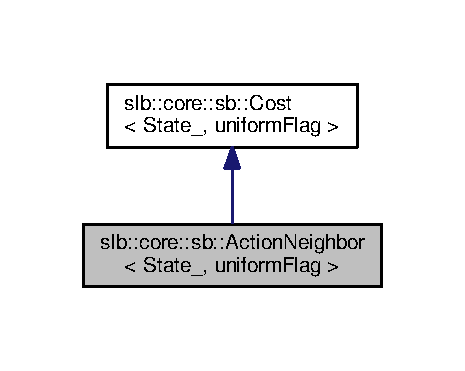
\includegraphics[width=223pt]{structslb_1_1core_1_1sb_1_1ActionNeighbor__inherit__graph}
\end{center}
\end{figure}


Collaboration diagram for slb\+:\+:core\+:\+:sb\+:\+:Action\+Neighbor$<$ State\+\_\+, uniform\+Flag $>$\+:\nopagebreak
\begin{figure}[H]
\begin{center}
\leavevmode
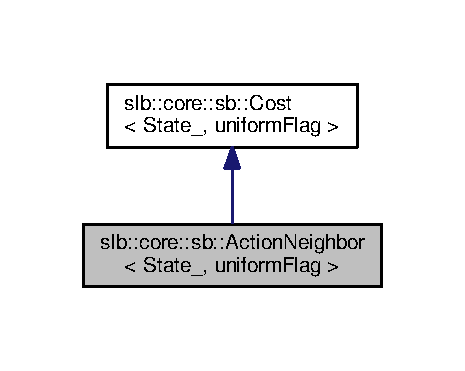
\includegraphics[width=223pt]{structslb_1_1core_1_1sb_1_1ActionNeighbor__coll__graph}
\end{center}
\end{figure}
\subsubsection*{Public Types}
\begin{DoxyCompactItemize}
\item 
using \hyperlink{structslb_1_1core_1_1sb_1_1ActionNeighbor_a02ad426b9f967a4dee5110053cd9c102}{State} = State\+\_\+\hypertarget{structslb_1_1core_1_1sb_1_1ActionNeighbor_a02ad426b9f967a4dee5110053cd9c102}{}\label{structslb_1_1core_1_1sb_1_1ActionNeighbor_a02ad426b9f967a4dee5110053cd9c102}

\begin{DoxyCompactList}\small\item\em The state type, represents the domain. \end{DoxyCompactList}\item 
using \hyperlink{structslb_1_1core_1_1sb_1_1ActionNeighbor_a6fcd3cfd6ae478c9a4751b051d2c01bd}{My\+Cost} = \hyperlink{structslb_1_1core_1_1sb_1_1Cost}{Cost}$<$ State\+\_\+, uniform\+Flag $>$\hypertarget{structslb_1_1core_1_1sb_1_1ActionNeighbor_a6fcd3cfd6ae478c9a4751b051d2c01bd}{}\label{structslb_1_1core_1_1sb_1_1ActionNeighbor_a6fcd3cfd6ae478c9a4751b051d2c01bd}

\begin{DoxyCompactList}\small\item\em Action cost type. \end{DoxyCompactList}\item 
using \hyperlink{structslb_1_1core_1_1sb_1_1ActionNeighbor_ae3ea9c18fb03dec73db239df85a86e57}{Action} = typename State\+::\+Action\hypertarget{structslb_1_1core_1_1sb_1_1ActionNeighbor_ae3ea9c18fb03dec73db239df85a86e57}{}\label{structslb_1_1core_1_1sb_1_1ActionNeighbor_ae3ea9c18fb03dec73db239df85a86e57}

\begin{DoxyCompactList}\small\item\em Action type. \end{DoxyCompactList}\item 
using \hyperlink{structslb_1_1core_1_1sb_1_1ActionNeighbor_a9e6b78876ab123703e20855fe79d6855}{Cost\+Type} = typename State\+::\+Cost\+Type\hypertarget{structslb_1_1core_1_1sb_1_1ActionNeighbor_a9e6b78876ab123703e20855fe79d6855}{}\label{structslb_1_1core_1_1sb_1_1ActionNeighbor_a9e6b78876ab123703e20855fe79d6855}

\begin{DoxyCompactList}\small\item\em Action cost type. \end{DoxyCompactList}\end{DoxyCompactItemize}
\subsubsection*{Public Member Functions}
\begin{DoxyCompactItemize}
\item 
\hyperlink{structslb_1_1core_1_1sb_1_1ActionNeighbor_ad022edd7e76461d64173c3531330c5af}{Action\+Neighbor} (\hyperlink{structslb_1_1core_1_1sb_1_1ActionNeighbor_ae3ea9c18fb03dec73db239df85a86e57}{Action} \&\&a, \hyperlink{structslb_1_1core_1_1sb_1_1Cost_a383726dcecbf69f396aa3a6d34b60278}{Cost\+Type} c=\hyperlink{structslb_1_1core_1_1sb_1_1Cost_a383726dcecbf69f396aa3a6d34b60278}{Cost\+Type}\{1\})
\begin{DoxyCompactList}\small\item\em Initializes the neighbor based on the neighbor state and cost of the action that leads to that state. \end{DoxyCompactList}\item 
const \hyperlink{structslb_1_1core_1_1sb_1_1ActionNeighbor_ae3ea9c18fb03dec73db239df85a86e57}{Action} \& \hyperlink{structslb_1_1core_1_1sb_1_1ActionNeighbor_aaaae0072af661ab1851132beca4cea3c}{action} () const 
\begin{DoxyCompactList}\small\item\em Returns the action. \end{DoxyCompactList}\end{DoxyCompactItemize}
\subsubsection*{Private Attributes}
\begin{DoxyCompactItemize}
\item 
\hyperlink{structslb_1_1core_1_1sb_1_1ActionNeighbor_ae3ea9c18fb03dec73db239df85a86e57}{Action} \hyperlink{structslb_1_1core_1_1sb_1_1ActionNeighbor_a2b653bb2c247e16fe4571fe56e6832d4}{a\+\_\+}\hypertarget{structslb_1_1core_1_1sb_1_1ActionNeighbor_a2b653bb2c247e16fe4571fe56e6832d4}{}\label{structslb_1_1core_1_1sb_1_1ActionNeighbor_a2b653bb2c247e16fe4571fe56e6832d4}

\begin{DoxyCompactList}\small\item\em The action. \end{DoxyCompactList}\end{DoxyCompactItemize}


\subsubsection{Detailed Description}
\subsubsection*{template$<$typename State\+\_\+, bool uniform\+Flag = true$>$\\*
struct slb\+::core\+::sb\+::\+Action\+Neighbor$<$ State\+\_\+, uniform\+Flag $>$}

The type for an action neighbor of a given state. 


\begin{DoxyTemplParams}{Template Parameters}
{\em State} & The state type, represents the domain. \\
\hline
{\em uniform\+Flag} & Determines whether the domain is a uniform cost one or not. \\
\hline
\end{DoxyTemplParams}


Definition at line 81 of file neighbor.\+h.



\subsubsection{Constructor \& Destructor Documentation}
\index{slb\+::core\+::sb\+::\+Action\+Neighbor@{slb\+::core\+::sb\+::\+Action\+Neighbor}!Action\+Neighbor@{Action\+Neighbor}}
\index{Action\+Neighbor@{Action\+Neighbor}!slb\+::core\+::sb\+::\+Action\+Neighbor@{slb\+::core\+::sb\+::\+Action\+Neighbor}}
\paragraph[{\texorpdfstring{Action\+Neighbor(\+Action \&\&a, Cost\+Type c=\+Cost\+Type\lcurly{}1\rcurly{})}{ActionNeighbor(Action &&a, CostType c=CostType\{1\})}}]{\setlength{\rightskip}{0pt plus 5cm}template$<$typename State\+\_\+ , bool uniform\+Flag = true$>$ {\bf slb\+::core\+::sb\+::\+Action\+Neighbor}$<$ State\+\_\+, uniform\+Flag $>$\+::{\bf Action\+Neighbor} (
\begin{DoxyParamCaption}
\item[{{\bf Action} \&\&}]{a, }
\item[{{\bf Cost\+Type}}]{c = {\ttfamily {\bf Cost\+Type}\{1\}}}
\end{DoxyParamCaption}
)\hspace{0.3cm}{\ttfamily [inline]}}\hypertarget{structslb_1_1core_1_1sb_1_1ActionNeighbor_ad022edd7e76461d64173c3531330c5af}{}\label{structslb_1_1core_1_1sb_1_1ActionNeighbor_ad022edd7e76461d64173c3531330c5af}


Initializes the neighbor based on the neighbor state and cost of the action that leads to that state. 


\begin{DoxyParams}{Parameters}
{\em a} & The action, which must be a right value. \\
\hline
{\em c} & \hyperlink{structslb_1_1core_1_1sb_1_1Cost}{Cost} of the action that leads to {\ttfamily s}. \\
\hline
\end{DoxyParams}


Definition at line 91 of file neighbor.\+h.



\subsubsection{Member Function Documentation}
\index{slb\+::core\+::sb\+::\+Action\+Neighbor@{slb\+::core\+::sb\+::\+Action\+Neighbor}!action@{action}}
\index{action@{action}!slb\+::core\+::sb\+::\+Action\+Neighbor@{slb\+::core\+::sb\+::\+Action\+Neighbor}}
\paragraph[{\texorpdfstring{action() const }{action() const }}]{\setlength{\rightskip}{0pt plus 5cm}template$<$typename State\+\_\+ , bool uniform\+Flag = true$>$ const {\bf Action}\& {\bf slb\+::core\+::sb\+::\+Action\+Neighbor}$<$ State\+\_\+, uniform\+Flag $>$\+::action (
\begin{DoxyParamCaption}
{}
\end{DoxyParamCaption}
) const\hspace{0.3cm}{\ttfamily [inline]}}\hypertarget{structslb_1_1core_1_1sb_1_1ActionNeighbor_aaaae0072af661ab1851132beca4cea3c}{}\label{structslb_1_1core_1_1sb_1_1ActionNeighbor_aaaae0072af661ab1851132beca4cea3c}


Returns the action. 

\begin{DoxyReturn}{Returns}
Const reference to the action. 
\end{DoxyReturn}


Definition at line 94 of file neighbor.\+h.



The documentation for this struct was generated from the following file\+:\begin{DoxyCompactItemize}
\item 
core/search\+\_\+base/\hyperlink{neighbor_8h}{neighbor.\+h}\end{DoxyCompactItemize}

\hypertarget{structslb_1_1ext_1_1policy_1_1generator_1_1ActionsT}{}\subsection{slb\+:\+:ext\+:\+:policy\+:\+:generator\+:\+:ActionsT$<$ My\+Algorithm, Heuristic $>$ Struct Template Reference}
\label{structslb_1_1ext_1_1policy_1_1generator_1_1ActionsT}\index{slb\+::ext\+::policy\+::generator\+::\+Actions\+T$<$ My\+Algorithm, Heuristic $>$@{slb\+::ext\+::policy\+::generator\+::\+Actions\+T$<$ My\+Algorithm, Heuristic $>$}}


Generator that generates action neighbors.  




{\ttfamily \#include $<$generators.\+h$>$}

\subsubsection*{Public Types}
\begin{DoxyCompactItemize}
\item 
using \hyperlink{structslb_1_1ext_1_1policy_1_1generator_1_1ActionsT_a579c1e623b0e091ad02ab78edb271810}{Neighbor} = typename State\+::\+A\+Neighbor\hypertarget{structslb_1_1ext_1_1policy_1_1generator_1_1ActionsT_a579c1e623b0e091ad02ab78edb271810}{}\label{structslb_1_1ext_1_1policy_1_1generator_1_1ActionsT_a579c1e623b0e091ad02ab78edb271810}

\begin{DoxyCompactList}\small\item\em The search neighbor type. \end{DoxyCompactList}\end{DoxyCompactItemize}
\subsubsection*{Public Member Functions}
\begin{DoxyCompactItemize}
\item 
\hyperlink{structslb_1_1ext_1_1policy_1_1generator_1_1ActionsT_a97a7c0421ba9ffe63a6790d46bd85c8d}{ActionsT} (My\+Algorithm \&alg)
\begin{DoxyCompactList}\small\item\em The contructor. \end{DoxyCompactList}\item 
State \hyperlink{structslb_1_1ext_1_1policy_1_1generator_1_1ActionsT_a85db41225282eb0fab196a7df5fb25e7}{state} (\hyperlink{structslb_1_1ext_1_1policy_1_1generator_1_1ActionsT_a579c1e623b0e091ad02ab78edb271810}{Neighbor} \&n) const 
\begin{DoxyCompactList}\small\item\em Returns the neighbor state. \end{DoxyCompactList}\item 
Cost\+Type \hyperlink{structslb_1_1ext_1_1policy_1_1generator_1_1ActionsT_af3ce8c0f1dd2b233fc0873a1757c17c9}{heuristic} (const \hyperlink{structslb_1_1ext_1_1policy_1_1generator_1_1ActionsT_a579c1e623b0e091ad02ab78edb271810}{Neighbor} \&n, Node $\ast$node) const 
\begin{DoxyCompactList}\small\item\em Computes the heuristic. \end{DoxyCompactList}\item 
std\+::vector$<$ \hyperlink{structslb_1_1ext_1_1policy_1_1generator_1_1ActionsT_a579c1e623b0e091ad02ab78edb271810}{Neighbor} $>$ \hyperlink{structslb_1_1ext_1_1policy_1_1generator_1_1ActionsT_a3aca825a8f5f7b647b12ed3aa33f6076}{successors} (const State \&s) const 
\begin{DoxyCompactList}\small\item\em Computes the successors of the given state. \end{DoxyCompactList}\end{DoxyCompactItemize}
\subsubsection*{Private Attributes}
\begin{DoxyCompactItemize}
\item 
My\+Algorithm \& \hyperlink{structslb_1_1ext_1_1policy_1_1generator_1_1ActionsT_ac7ba713fd6922437044de0ac81c3df6b}{alg\+\_\+}\hypertarget{structslb_1_1ext_1_1policy_1_1generator_1_1ActionsT_ac7ba713fd6922437044de0ac81c3df6b}{}\label{structslb_1_1ext_1_1policy_1_1generator_1_1ActionsT_ac7ba713fd6922437044de0ac81c3df6b}

\begin{DoxyCompactList}\small\item\em Reference to the search algorithm. \end{DoxyCompactList}\item 
Heuristic$<$ My\+Algorithm $>$ \hyperlink{structslb_1_1ext_1_1policy_1_1generator_1_1ActionsT_a9f44dbf470dd772315d21c4a94d22167}{heuristic\+\_\+}\hypertarget{structslb_1_1ext_1_1policy_1_1generator_1_1ActionsT_a9f44dbf470dd772315d21c4a94d22167}{}\label{structslb_1_1ext_1_1policy_1_1generator_1_1ActionsT_a9f44dbf470dd772315d21c4a94d22167}

\begin{DoxyCompactList}\small\item\em The heuristic. \end{DoxyCompactList}\end{DoxyCompactItemize}


\subsubsection{Detailed Description}
\subsubsection*{template$<$class My\+Algorithm, template$<$ class $>$ class Heuristic$>$\\*
struct slb\+::ext\+::policy\+::generator\+::\+Actions\+T$<$ My\+Algorithm, Heuristic $>$}

Generator that generates action neighbors. 


\begin{DoxyTemplParams}{Template Parameters}
{\em My\+Algorithm} & The search algorithm. \\
\hline
{\em Heuristic} & The heuristic policy. \\
\hline
\end{DoxyTemplParams}


Definition at line 66 of file generators.\+h.



\subsubsection{Constructor \& Destructor Documentation}
\index{slb\+::ext\+::policy\+::generator\+::\+ActionsT@{slb\+::ext\+::policy\+::generator\+::\+ActionsT}!ActionsT@{ActionsT}}
\index{ActionsT@{ActionsT}!slb\+::ext\+::policy\+::generator\+::\+ActionsT@{slb\+::ext\+::policy\+::generator\+::\+ActionsT}}
\paragraph[{\texorpdfstring{Actions\+T(\+My\+Algorithm \&alg)}{ActionsT(MyAlgorithm &alg)}}]{\setlength{\rightskip}{0pt plus 5cm}template$<$class My\+Algorithm , template$<$ class $>$ class Heuristic$>$ {\bf slb\+::ext\+::policy\+::generator\+::\+ActionsT}$<$ My\+Algorithm, Heuristic $>$\+::{\bf ActionsT} (
\begin{DoxyParamCaption}
\item[{My\+Algorithm \&}]{alg}
\end{DoxyParamCaption}
)\hspace{0.3cm}{\ttfamily [inline]}}\hypertarget{structslb_1_1ext_1_1policy_1_1generator_1_1ActionsT_a97a7c0421ba9ffe63a6790d46bd85c8d}{}\label{structslb_1_1ext_1_1policy_1_1generator_1_1ActionsT_a97a7c0421ba9ffe63a6790d46bd85c8d}


The contructor. 


\begin{DoxyParams}{Parameters}
{\em alg} & Reference to the search algorithm. \\
\hline
\end{DoxyParams}


Definition at line 74 of file generators.\+h.



\subsubsection{Member Function Documentation}
\index{slb\+::ext\+::policy\+::generator\+::\+ActionsT@{slb\+::ext\+::policy\+::generator\+::\+ActionsT}!heuristic@{heuristic}}
\index{heuristic@{heuristic}!slb\+::ext\+::policy\+::generator\+::\+ActionsT@{slb\+::ext\+::policy\+::generator\+::\+ActionsT}}
\paragraph[{\texorpdfstring{heuristic(const Neighbor \&n, Node $\ast$node) const }{heuristic(const Neighbor &n, Node *node) const }}]{\setlength{\rightskip}{0pt plus 5cm}template$<$class My\+Algorithm , template$<$ class $>$ class Heuristic$>$ Cost\+Type {\bf slb\+::ext\+::policy\+::generator\+::\+ActionsT}$<$ My\+Algorithm, Heuristic $>$\+::heuristic (
\begin{DoxyParamCaption}
\item[{const {\bf Neighbor} \&}]{n, }
\item[{Node $\ast$}]{node}
\end{DoxyParamCaption}
) const\hspace{0.3cm}{\ttfamily [inline]}}\hypertarget{structslb_1_1ext_1_1policy_1_1generator_1_1ActionsT_af3ce8c0f1dd2b233fc0873a1757c17c9}{}\label{structslb_1_1ext_1_1policy_1_1generator_1_1ActionsT_af3ce8c0f1dd2b233fc0873a1757c17c9}


Computes the heuristic. 


\begin{DoxyParams}{Parameters}
{\em n} & The neighbor for which the heuristic is to be computed. \\
\hline
{\em node} & The search node for which the heuristic is to be computed. \\
\hline
\end{DoxyParams}
\begin{DoxyReturn}{Returns}
The heuristic value. 
\end{DoxyReturn}


Definition at line 88 of file generators.\+h.

\index{slb\+::ext\+::policy\+::generator\+::\+ActionsT@{slb\+::ext\+::policy\+::generator\+::\+ActionsT}!state@{state}}
\index{state@{state}!slb\+::ext\+::policy\+::generator\+::\+ActionsT@{slb\+::ext\+::policy\+::generator\+::\+ActionsT}}
\paragraph[{\texorpdfstring{state(\+Neighbor \&n) const }{state(Neighbor &n) const }}]{\setlength{\rightskip}{0pt plus 5cm}template$<$class My\+Algorithm , template$<$ class $>$ class Heuristic$>$ State {\bf slb\+::ext\+::policy\+::generator\+::\+ActionsT}$<$ My\+Algorithm, Heuristic $>$\+::state (
\begin{DoxyParamCaption}
\item[{{\bf Neighbor} \&}]{n}
\end{DoxyParamCaption}
) const\hspace{0.3cm}{\ttfamily [inline]}}\hypertarget{structslb_1_1ext_1_1policy_1_1generator_1_1ActionsT_a85db41225282eb0fab196a7df5fb25e7}{}\label{structslb_1_1ext_1_1policy_1_1generator_1_1ActionsT_a85db41225282eb0fab196a7df5fb25e7}


Returns the neighbor state. 

\begin{DoxyReturn}{Returns}
Reference to the neighbor state. 
\end{DoxyReturn}
\begin{DoxyNote}{Note}
This reference must be non-\/const to allow moving the neighbor 
\end{DoxyNote}


Definition at line 79 of file generators.\+h.

\index{slb\+::ext\+::policy\+::generator\+::\+ActionsT@{slb\+::ext\+::policy\+::generator\+::\+ActionsT}!successors@{successors}}
\index{successors@{successors}!slb\+::ext\+::policy\+::generator\+::\+ActionsT@{slb\+::ext\+::policy\+::generator\+::\+ActionsT}}
\paragraph[{\texorpdfstring{successors(const State \&s) const }{successors(const State &s) const }}]{\setlength{\rightskip}{0pt plus 5cm}template$<$class My\+Algorithm , template$<$ class $>$ class Heuristic$>$ std\+::vector$<${\bf Neighbor}$>$ {\bf slb\+::ext\+::policy\+::generator\+::\+ActionsT}$<$ My\+Algorithm, Heuristic $>$\+::successors (
\begin{DoxyParamCaption}
\item[{const State \&}]{s}
\end{DoxyParamCaption}
) const\hspace{0.3cm}{\ttfamily [inline]}}\hypertarget{structslb_1_1ext_1_1policy_1_1generator_1_1ActionsT_a3aca825a8f5f7b647b12ed3aa33f6076}{}\label{structslb_1_1ext_1_1policy_1_1generator_1_1ActionsT_a3aca825a8f5f7b647b12ed3aa33f6076}


Computes the successors of the given state. 


\begin{DoxyParams}{Parameters}
{\em s} & The state. \\
\hline
\end{DoxyParams}
\begin{DoxyReturn}{Returns}
The vector of successors. 
\end{DoxyReturn}
\begin{DoxyNote}{Note}
This member could be static; made it non-\/static for reasons of uniformity. 
\end{DoxyNote}


Definition at line 97 of file generators.\+h.



The documentation for this struct was generated from the following file\+:\begin{DoxyCompactItemize}
\item 
extensions/shared\+\_\+policies/\hyperlink{generators_8h}{generators.\+h}\end{DoxyCompactItemize}

\hypertarget{structslb_1_1ext_1_1algorithm_1_1Algorithm}{}\subsection{slb\+:\+:ext\+:\+:algorithm\+:\+:Algorithm$<$ Concrete, A\+L\+G\+\_\+\+T\+P\+A\+R\+A\+MS $>$ Struct Template Reference}
\label{structslb_1_1ext_1_1algorithm_1_1Algorithm}\index{slb\+::ext\+::algorithm\+::\+Algorithm$<$ Concrete, A\+L\+G\+\_\+\+T\+P\+A\+R\+A\+M\+S $>$@{slb\+::ext\+::algorithm\+::\+Algorithm$<$ Concrete, A\+L\+G\+\_\+\+T\+P\+A\+R\+A\+M\+S $>$}}


Abstract base for search algorithms.  




{\ttfamily \#include $<$algorithm.\+h$>$}



Collaboration diagram for slb\+:\+:ext\+:\+:algorithm\+:\+:Algorithm$<$ Concrete, A\+L\+G\+\_\+\+T\+P\+A\+R\+A\+MS $>$\+:\nopagebreak
\begin{figure}[H]
\begin{center}
\leavevmode
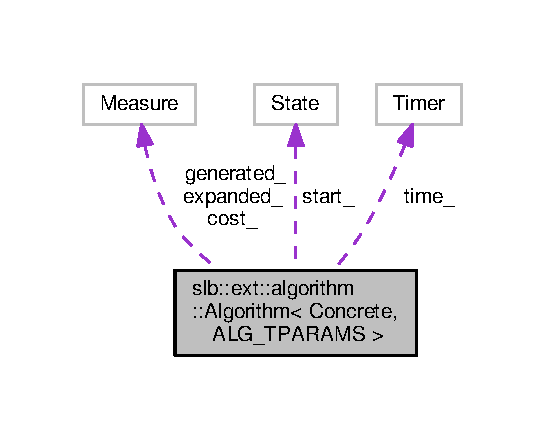
\includegraphics[width=262pt]{structslb_1_1ext_1_1algorithm_1_1Algorithm__coll__graph}
\end{center}
\end{figure}
\subsubsection*{Public Types}
\begin{DoxyCompactItemize}
\item 
using \hyperlink{structslb_1_1ext_1_1algorithm_1_1Algorithm_ae0c6a75028107e4642e43798f21f4bfc}{Goal\+Handler} = Goal\+Handler\+\_\+$<$ Concrete $>$\hypertarget{structslb_1_1ext_1_1algorithm_1_1Algorithm_ae0c6a75028107e4642e43798f21f4bfc}{}\label{structslb_1_1ext_1_1algorithm_1_1Algorithm_ae0c6a75028107e4642e43798f21f4bfc}

\begin{DoxyCompactList}\small\item\em The goal handler policy type. \end{DoxyCompactList}\item 
using \hyperlink{structslb_1_1ext_1_1algorithm_1_1Algorithm_ad1f8f28e7b07f747ef7b7b5bf0643c2d}{Initial\+Heuristic} = Initial\+Heuristic\+\_\+$<$ Concrete $>$\hypertarget{structslb_1_1ext_1_1algorithm_1_1Algorithm_ad1f8f28e7b07f747ef7b7b5bf0643c2d}{}\label{structslb_1_1ext_1_1algorithm_1_1Algorithm_ad1f8f28e7b07f747ef7b7b5bf0643c2d}

\begin{DoxyCompactList}\small\item\em The initial heuristic policy type. \end{DoxyCompactList}\item 
using \hyperlink{structslb_1_1ext_1_1algorithm_1_1Algorithm_afa5a78c048b4fe4f5848aeaf5c1f8d65}{Generator} = Generator\+\_\+$<$ Concrete $>$\hypertarget{structslb_1_1ext_1_1algorithm_1_1Algorithm_afa5a78c048b4fe4f5848aeaf5c1f8d65}{}\label{structslb_1_1ext_1_1algorithm_1_1Algorithm_afa5a78c048b4fe4f5848aeaf5c1f8d65}

\begin{DoxyCompactList}\small\item\em The generator policy type. \end{DoxyCompactList}\end{DoxyCompactItemize}
\subsubsection*{Public Member Functions}
\begin{DoxyCompactItemize}
\item 
\hyperlink{structslb_1_1core_1_1sb_1_1MeasureSet}{Measure\+Set} \hyperlink{structslb_1_1ext_1_1algorithm_1_1Algorithm_a539d8d4e7d92ed9a80c778b530754c13}{measures} () const 
\begin{DoxyCompactList}\small\item\em Returns the statistics about the search algorithm\textquotesingle{}s performance for solving the particular instance. \end{DoxyCompactList}\item 
My\+Algorithm\+Log \& \hyperlink{structslb_1_1ext_1_1algorithm_1_1Algorithm_aa8adc2ad3941377d1b34e92ff66d2c6a}{log} ()
\begin{DoxyCompactList}\small\item\em Returns the log of events generated by the search algorithm. \end{DoxyCompactList}\end{DoxyCompactItemize}
\begin{Indent}{\bf Services for policies.}\par
\begin{DoxyCompactItemize}
\item 
My\+Instance \& {\bfseries instance} ()\hypertarget{structslb_1_1ext_1_1algorithm_1_1Algorithm_a12672baeccfa80b4e58507fcce64cb03}{}\label{structslb_1_1ext_1_1algorithm_1_1Algorithm_a12672baeccfa80b4e58507fcce64cb03}

\item 
\hyperlink{structslb_1_1ext_1_1algorithm_1_1Algorithm_ae0c6a75028107e4642e43798f21f4bfc}{Goal\+Handler} \& {\bfseries goal\+Handler} ()\hypertarget{structslb_1_1ext_1_1algorithm_1_1Algorithm_a02c455c8bb8d23a1b57d2031c1dc7765}{}\label{structslb_1_1ext_1_1algorithm_1_1Algorithm_a02c455c8bb8d23a1b57d2031c1dc7765}

\item 
\hyperlink{structslb_1_1ext_1_1algorithm_1_1Algorithm_ad1f8f28e7b07f747ef7b7b5bf0643c2d}{Initial\+Heuristic} \& {\bfseries inital\+Heuristic} ()\hypertarget{structslb_1_1ext_1_1algorithm_1_1Algorithm_aacffe484619751d9d15ffa36801d5243}{}\label{structslb_1_1ext_1_1algorithm_1_1Algorithm_aacffe484619751d9d15ffa36801d5243}

\item 
\hyperlink{structslb_1_1ext_1_1algorithm_1_1Algorithm_afa5a78c048b4fe4f5848aeaf5c1f8d65}{Generator} \& {\bfseries generator} ()\hypertarget{structslb_1_1ext_1_1algorithm_1_1Algorithm_a7d3fb914e7abe4758a17ba29b6ff9e51}{}\label{structslb_1_1ext_1_1algorithm_1_1Algorithm_a7d3fb914e7abe4758a17ba29b6ff9e51}

\item 
int \hyperlink{structslb_1_1ext_1_1algorithm_1_1Algorithm_ae8584fe237904c9e6f3b88adab11032a}{stamp} ()
\begin{DoxyCompactList}\small\item\em Returns the current time stamp of the search algorithm. The number of generated nodes is currently used as the stamp. \end{DoxyCompactList}\item 
Return\+Type \& \hyperlink{structslb_1_1ext_1_1algorithm_1_1Algorithm_a263f4d05670e313ee8660e872dae4462}{res} ()
\begin{DoxyCompactList}\small\item\em Returns reference to the result. \end{DoxyCompactList}\end{DoxyCompactItemize}
\end{Indent}
\subsubsection*{Static Public Attributes}
\begin{DoxyCompactItemize}
\item 
static \hyperlink{algorithm_8h_af9ce42dc0033d5c93cea8af7002ab583}{B\+A\+S\+E\+\_\+\+T\+R\+A\+I\+T\+S\+\_\+\+T\+Y\+P\+ES} constexpr bool \hyperlink{structslb_1_1ext_1_1algorithm_1_1Algorithm_a614bd0faf9d0eba04f45bb204afac021}{log\+Flag} = log\+Flag\+\_\+\hypertarget{structslb_1_1ext_1_1algorithm_1_1Algorithm_a614bd0faf9d0eba04f45bb204afac021}{}\label{structslb_1_1ext_1_1algorithm_1_1Algorithm_a614bd0faf9d0eba04f45bb204afac021}

\begin{DoxyCompactList}\small\item\em {\ttfamily true} if the events generated by the search algorithm are logged and {\ttfamily false} otherwise. \end{DoxyCompactList}\end{DoxyCompactItemize}
\subsubsection*{Protected Member Functions}
\begin{DoxyCompactItemize}
\item 
\hyperlink{structslb_1_1ext_1_1algorithm_1_1Algorithm_a1569912641a50ba140907372462177cf}{Algorithm} (const My\+Instance \&instance)
\begin{DoxyCompactList}\small\item\em Initializes the algorithm based on the problem instance. \end{DoxyCompactList}\end{DoxyCompactItemize}
\subsubsection*{Protected Attributes}
\begin{DoxyCompactItemize}
\item 
My\+Instance \hyperlink{structslb_1_1ext_1_1algorithm_1_1Algorithm_a2924c26498dd2658fa0cc20a47f78d0d}{instance\+\_\+}\hypertarget{structslb_1_1ext_1_1algorithm_1_1Algorithm_a2924c26498dd2658fa0cc20a47f78d0d}{}\label{structslb_1_1ext_1_1algorithm_1_1Algorithm_a2924c26498dd2658fa0cc20a47f78d0d}

\begin{DoxyCompactList}\small\item\em The problem instance. \end{DoxyCompactList}\item 
My\+Algorithm\+Log \hyperlink{structslb_1_1ext_1_1algorithm_1_1Algorithm_aa63e4ab3a6f3b2632320018760c923fd}{log\+\_\+}\hypertarget{structslb_1_1ext_1_1algorithm_1_1Algorithm_aa63e4ab3a6f3b2632320018760c923fd}{}\label{structslb_1_1ext_1_1algorithm_1_1Algorithm_aa63e4ab3a6f3b2632320018760c923fd}

\begin{DoxyCompactList}\small\item\em The log of events generated by the search algorithm. \end{DoxyCompactList}\item 
State \hyperlink{structslb_1_1ext_1_1algorithm_1_1Algorithm_a202dfe3bac28cb6a97246d378080f704}{start\+\_\+}\hypertarget{structslb_1_1ext_1_1algorithm_1_1Algorithm_a202dfe3bac28cb6a97246d378080f704}{}\label{structslb_1_1ext_1_1algorithm_1_1Algorithm_a202dfe3bac28cb6a97246d378080f704}

\begin{DoxyCompactList}\small\item\em The start state (multiple start states are to be handled in the future). \end{DoxyCompactList}\item 
\hyperlink{structslb_1_1ext_1_1algorithm_1_1Algorithm_ae0c6a75028107e4642e43798f21f4bfc}{Goal\+Handler} \hyperlink{structslb_1_1ext_1_1algorithm_1_1Algorithm_a88c9b86bd51e50df1f2da840eed1ec46}{goal\+Handler\+\_\+}\hypertarget{structslb_1_1ext_1_1algorithm_1_1Algorithm_a88c9b86bd51e50df1f2da840eed1ec46}{}\label{structslb_1_1ext_1_1algorithm_1_1Algorithm_a88c9b86bd51e50df1f2da840eed1ec46}

\begin{DoxyCompactList}\small\item\em The policy for handling conditions related to goal states. \end{DoxyCompactList}\item 
\hyperlink{structslb_1_1ext_1_1algorithm_1_1Algorithm_ad1f8f28e7b07f747ef7b7b5bf0643c2d}{Initial\+Heuristic} \hyperlink{structslb_1_1ext_1_1algorithm_1_1Algorithm_a21c643fd7b13c678ee91ad70203148bb}{initial\+Heuristic\+\_\+}\hypertarget{structslb_1_1ext_1_1algorithm_1_1Algorithm_a21c643fd7b13c678ee91ad70203148bb}{}\label{structslb_1_1ext_1_1algorithm_1_1Algorithm_a21c643fd7b13c678ee91ad70203148bb}

\begin{DoxyCompactList}\small\item\em The initial heuristic used by the search algorithm. \end{DoxyCompactList}\item 
\hyperlink{structslb_1_1ext_1_1algorithm_1_1Algorithm_afa5a78c048b4fe4f5848aeaf5c1f8d65}{Generator} \hyperlink{structslb_1_1ext_1_1algorithm_1_1Algorithm_ae5ba008ce8869dbcb55be0af9ca9f129}{generator\+\_\+}\hypertarget{structslb_1_1ext_1_1algorithm_1_1Algorithm_ae5ba008ce8869dbcb55be0af9ca9f129}{}\label{structslb_1_1ext_1_1algorithm_1_1Algorithm_ae5ba008ce8869dbcb55be0af9ca9f129}

\begin{DoxyCompactList}\small\item\em The generator used by the search algorithm. \end{DoxyCompactList}\end{DoxyCompactItemize}
\begin{Indent}{\bf Statistics about the search algorithm\textquotesingle{}s performance.}\par
{\em \begin{DoxyNote}{Note}
These statistics pertain to solving the particular instance. 
\end{DoxyNote}
}\begin{DoxyCompactItemize}
\item 
Measure \hyperlink{structslb_1_1ext_1_1algorithm_1_1Algorithm_a5d6d2b982578359c96d1276ac217e2ce}{expanded\+\_\+} \{\char`\"{}Expanded\char`\"{}\}\hypertarget{structslb_1_1ext_1_1algorithm_1_1Algorithm_a5d6d2b982578359c96d1276ac217e2ce}{}\label{structslb_1_1ext_1_1algorithm_1_1Algorithm_a5d6d2b982578359c96d1276ac217e2ce}

\begin{DoxyCompactList}\small\item\em The number of nodes expanded by the search algorithm. \end{DoxyCompactList}\item 
Measure \hyperlink{structslb_1_1ext_1_1algorithm_1_1Algorithm_ad8b051ee61ed7b4ac6337015f4f43ada}{generated\+\_\+} \{\char`\"{}Generated\char`\"{}\}\hypertarget{structslb_1_1ext_1_1algorithm_1_1Algorithm_ad8b051ee61ed7b4ac6337015f4f43ada}{}\label{structslb_1_1ext_1_1algorithm_1_1Algorithm_ad8b051ee61ed7b4ac6337015f4f43ada}

\begin{DoxyCompactList}\small\item\em The number of nodes generated by the search algorithm. \end{DoxyCompactList}\item 
Timer \hyperlink{structslb_1_1ext_1_1algorithm_1_1Algorithm_aa2b6a06d38134130e502ffc79ee6cb97}{time\+\_\+} \{\char`\"{}Time (ms.)\char`\"{}\}\hypertarget{structslb_1_1ext_1_1algorithm_1_1Algorithm_aa2b6a06d38134130e502ffc79ee6cb97}{}\label{structslb_1_1ext_1_1algorithm_1_1Algorithm_aa2b6a06d38134130e502ffc79ee6cb97}

\begin{DoxyCompactList}\small\item\em Time taken by the search algorithm. \end{DoxyCompactList}\item 
Measure \hyperlink{structslb_1_1ext_1_1algorithm_1_1Algorithm_a1d610112ac4f8f5a28c06a40a9c9c5ce}{cost\+\_\+} \{\char`\"{}Cost\char`\"{}\}\hypertarget{structslb_1_1ext_1_1algorithm_1_1Algorithm_a1d610112ac4f8f5a28c06a40a9c9c5ce}{}\label{structslb_1_1ext_1_1algorithm_1_1Algorithm_a1d610112ac4f8f5a28c06a40a9c9c5ce}

\begin{DoxyCompactList}\small\item\em The cost of the solution. \end{DoxyCompactList}\item 
Return\+Type \hyperlink{structslb_1_1ext_1_1algorithm_1_1Algorithm_ac01ce5a7230cbc835507bfc00d37fe5d}{res\+\_\+} \{-\/1\}\hypertarget{structslb_1_1ext_1_1algorithm_1_1Algorithm_ac01ce5a7230cbc835507bfc00d37fe5d}{}\label{structslb_1_1ext_1_1algorithm_1_1Algorithm_ac01ce5a7230cbc835507bfc00d37fe5d}

\begin{DoxyCompactList}\small\item\em The solution cost. -\/1 stands for no solution. \end{DoxyCompactList}\end{DoxyCompactItemize}
\end{Indent}


\subsubsection{Detailed Description}
\subsubsection*{template$<$class Concrete, A\+L\+G\+\_\+\+T\+P\+A\+R\+A\+MS$>$\\*
struct slb\+::ext\+::algorithm\+::\+Algorithm$<$ Concrete, A\+L\+G\+\_\+\+T\+P\+A\+R\+A\+M\+S $>$}

Abstract base for search algorithms. 


\begin{DoxyTemplParams}{Template Parameters}
{\em log\+Flag\+\_\+} & If {\ttfamily true}, the events generated by the search algorithm are logged. Otherwise, they are not. \\
\hline
{\em Node\+\_\+} & The search node type. \\
\hline
{\em Goal\+Handler} & The policy for handling goal conditions. \\
\hline
{\em Heuristic} & The heuristic used by the search algorithm. \\
\hline
{\em Generator} & The generator used by the search algorithm. \\
\hline
\end{DoxyTemplParams}


Definition at line 108 of file algorithm.\+h.



\subsubsection{Constructor \& Destructor Documentation}
\index{slb\+::ext\+::algorithm\+::\+Algorithm@{slb\+::ext\+::algorithm\+::\+Algorithm}!Algorithm@{Algorithm}}
\index{Algorithm@{Algorithm}!slb\+::ext\+::algorithm\+::\+Algorithm@{slb\+::ext\+::algorithm\+::\+Algorithm}}
\paragraph[{\texorpdfstring{Algorithm(const My\+Instance \&instance)}{Algorithm(const MyInstance &instance)}}]{\setlength{\rightskip}{0pt plus 5cm}template$<$class Concrete, A\+L\+G\+\_\+\+T\+P\+A\+R\+A\+MS $>$ {\bf slb\+::ext\+::algorithm\+::\+Algorithm}$<$ Concrete, {\bf A\+L\+G\+\_\+\+T\+P\+A\+R\+A\+MS} $>$\+::{\bf Algorithm} (
\begin{DoxyParamCaption}
\item[{const My\+Instance \&}]{instance}
\end{DoxyParamCaption}
)\hspace{0.3cm}{\ttfamily [inline]}, {\ttfamily [protected]}}\hypertarget{structslb_1_1ext_1_1algorithm_1_1Algorithm_a1569912641a50ba140907372462177cf}{}\label{structslb_1_1ext_1_1algorithm_1_1Algorithm_a1569912641a50ba140907372462177cf}


Initializes the algorithm based on the problem instance. 


\begin{DoxyParams}{Parameters}
{\em instance} & The problem instance. \\
\hline
\end{DoxyParams}


Definition at line 161 of file algorithm.\+h.



\subsubsection{Member Function Documentation}
\index{slb\+::ext\+::algorithm\+::\+Algorithm@{slb\+::ext\+::algorithm\+::\+Algorithm}!log@{log}}
\index{log@{log}!slb\+::ext\+::algorithm\+::\+Algorithm@{slb\+::ext\+::algorithm\+::\+Algorithm}}
\paragraph[{\texorpdfstring{log()}{log()}}]{\setlength{\rightskip}{0pt plus 5cm}template$<$class Concrete, A\+L\+G\+\_\+\+T\+P\+A\+R\+A\+MS $>$ My\+Algorithm\+Log\& {\bf slb\+::ext\+::algorithm\+::\+Algorithm}$<$ Concrete, {\bf A\+L\+G\+\_\+\+T\+P\+A\+R\+A\+MS} $>$\+::log (
\begin{DoxyParamCaption}
{}
\end{DoxyParamCaption}
)\hspace{0.3cm}{\ttfamily [inline]}}\hypertarget{structslb_1_1ext_1_1algorithm_1_1Algorithm_aa8adc2ad3941377d1b34e92ff66d2c6a}{}\label{structslb_1_1ext_1_1algorithm_1_1Algorithm_aa8adc2ad3941377d1b34e92ff66d2c6a}


Returns the log of events generated by the search algorithm. 

\begin{DoxyReturn}{Returns}
Const reference to the log of events generated by the search algorithm. 
\end{DoxyReturn}


Definition at line 138 of file algorithm.\+h.

\index{slb\+::ext\+::algorithm\+::\+Algorithm@{slb\+::ext\+::algorithm\+::\+Algorithm}!measures@{measures}}
\index{measures@{measures}!slb\+::ext\+::algorithm\+::\+Algorithm@{slb\+::ext\+::algorithm\+::\+Algorithm}}
\paragraph[{\texorpdfstring{measures() const }{measures() const }}]{\setlength{\rightskip}{0pt plus 5cm}template$<$class Concrete, A\+L\+G\+\_\+\+T\+P\+A\+R\+A\+MS $>$ {\bf Measure\+Set} {\bf slb\+::ext\+::algorithm\+::\+Algorithm}$<$ Concrete, {\bf A\+L\+G\+\_\+\+T\+P\+A\+R\+A\+MS} $>$\+::measures (
\begin{DoxyParamCaption}
{}
\end{DoxyParamCaption}
) const\hspace{0.3cm}{\ttfamily [inline]}}\hypertarget{structslb_1_1ext_1_1algorithm_1_1Algorithm_a539d8d4e7d92ed9a80c778b530754c13}{}\label{structslb_1_1ext_1_1algorithm_1_1Algorithm_a539d8d4e7d92ed9a80c778b530754c13}


Returns the statistics about the search algorithm\textquotesingle{}s performance for solving the particular instance. 

\begin{DoxyReturn}{Returns}
The statistics about the search algorithm\textquotesingle{}s performance for solving the particular instance. 
\end{DoxyReturn}


Definition at line 131 of file algorithm.\+h.

\index{slb\+::ext\+::algorithm\+::\+Algorithm@{slb\+::ext\+::algorithm\+::\+Algorithm}!res@{res}}
\index{res@{res}!slb\+::ext\+::algorithm\+::\+Algorithm@{slb\+::ext\+::algorithm\+::\+Algorithm}}
\paragraph[{\texorpdfstring{res()}{res()}}]{\setlength{\rightskip}{0pt plus 5cm}template$<$class Concrete, A\+L\+G\+\_\+\+T\+P\+A\+R\+A\+MS $>$ Return\+Type\& {\bf slb\+::ext\+::algorithm\+::\+Algorithm}$<$ Concrete, {\bf A\+L\+G\+\_\+\+T\+P\+A\+R\+A\+MS} $>$\+::res (
\begin{DoxyParamCaption}
{}
\end{DoxyParamCaption}
)\hspace{0.3cm}{\ttfamily [inline]}}\hypertarget{structslb_1_1ext_1_1algorithm_1_1Algorithm_a263f4d05670e313ee8660e872dae4462}{}\label{structslb_1_1ext_1_1algorithm_1_1Algorithm_a263f4d05670e313ee8660e872dae4462}


Returns reference to the result. 

\begin{DoxyReturn}{Returns}
Reference to the result. 
\end{DoxyReturn}


Definition at line 155 of file algorithm.\+h.

\index{slb\+::ext\+::algorithm\+::\+Algorithm@{slb\+::ext\+::algorithm\+::\+Algorithm}!stamp@{stamp}}
\index{stamp@{stamp}!slb\+::ext\+::algorithm\+::\+Algorithm@{slb\+::ext\+::algorithm\+::\+Algorithm}}
\paragraph[{\texorpdfstring{stamp()}{stamp()}}]{\setlength{\rightskip}{0pt plus 5cm}template$<$class Concrete, A\+L\+G\+\_\+\+T\+P\+A\+R\+A\+MS $>$ int {\bf slb\+::ext\+::algorithm\+::\+Algorithm}$<$ Concrete, {\bf A\+L\+G\+\_\+\+T\+P\+A\+R\+A\+MS} $>$\+::stamp (
\begin{DoxyParamCaption}
{}
\end{DoxyParamCaption}
)\hspace{0.3cm}{\ttfamily [inline]}}\hypertarget{structslb_1_1ext_1_1algorithm_1_1Algorithm_ae8584fe237904c9e6f3b88adab11032a}{}\label{structslb_1_1ext_1_1algorithm_1_1Algorithm_ae8584fe237904c9e6f3b88adab11032a}


Returns the current time stamp of the search algorithm. The number of generated nodes is currently used as the stamp. 

\begin{DoxyReturn}{Returns}
The current time stamp of the search algorithm. 
\end{DoxyReturn}


Definition at line 151 of file algorithm.\+h.



The documentation for this struct was generated from the following file\+:\begin{DoxyCompactItemize}
\item 
extensions/algorithms/\hyperlink{algorithm_8h}{algorithm.\+h}\end{DoxyCompactItemize}

\hypertarget{structslb_1_1core_1_1ui_1_1AlgorithmLog}{}\subsection{slb\+:\+:core\+:\+:ui\+:\+:Algorithm\+Log$<$ Node $>$ Struct Template Reference}
\label{structslb_1_1core_1_1ui_1_1AlgorithmLog}\index{slb\+::core\+::ui\+::\+Algorithm\+Log$<$ Node $>$@{slb\+::core\+::ui\+::\+Algorithm\+Log$<$ Node $>$}}


The log of events generated by an algorithm.  




{\ttfamily \#include $<$algorithm\+\_\+log.\+h$>$}

\subsubsection*{Public Types}
\begin{DoxyCompactItemize}
\item 
using \hyperlink{structslb_1_1core_1_1ui_1_1AlgorithmLog_aa495893d6c587c69280c82dd4f1684ff}{Event} = std\+::shared\+\_\+ptr$<$ \hyperlink{structslb_1_1core_1_1ui_1_1EventBase}{Event\+Base}$<$ Node $>$$>$\hypertarget{structslb_1_1core_1_1ui_1_1AlgorithmLog_aa495893d6c587c69280c82dd4f1684ff}{}\label{structslb_1_1core_1_1ui_1_1AlgorithmLog_aa495893d6c587c69280c82dd4f1684ff}

\begin{DoxyCompactList}\small\item\em Smart pointer to an event generated by the algorithm. \end{DoxyCompactList}\item 
using \hyperlink{structslb_1_1core_1_1ui_1_1AlgorithmLog_ac9bad13ba3a1f7a8d1b545a86897b0b4}{State} = typename Node\+::\+State\hypertarget{structslb_1_1core_1_1ui_1_1AlgorithmLog_ac9bad13ba3a1f7a8d1b545a86897b0b4}{}\label{structslb_1_1core_1_1ui_1_1AlgorithmLog_ac9bad13ba3a1f7a8d1b545a86897b0b4}

\begin{DoxyCompactList}\small\item\em The state type, represents the domain. \end{DoxyCompactList}\item 
using \hyperlink{structslb_1_1core_1_1ui_1_1AlgorithmLog_acb46cb3c44c97ddbb219e4c0120e87e3}{State\+Shared\+Ptr} = \hyperlink{classslb_1_1core_1_1util_1_1deref__shared__ptr}{deref\+\_\+shared\+\_\+ptr}$<$ const \hyperlink{structslb_1_1core_1_1ui_1_1AlgorithmLog_ac9bad13ba3a1f7a8d1b545a86897b0b4}{State} $>$\hypertarget{structslb_1_1core_1_1ui_1_1AlgorithmLog_acb46cb3c44c97ddbb219e4c0120e87e3}{}\label{structslb_1_1core_1_1ui_1_1AlgorithmLog_acb46cb3c44c97ddbb219e4c0120e87e3}

\begin{DoxyCompactList}\small\item\em Smart pointer to state. \end{DoxyCompactList}\end{DoxyCompactItemize}
\subsubsection*{Public Member Functions}
\begin{DoxyCompactItemize}
\item 
void \hyperlink{structslb_1_1core_1_1ui_1_1AlgorithmLog_aeedd840e2ae69d8e581b55f4fa36268a}{log} (const \hyperlink{structslb_1_1core_1_1ui_1_1AlgorithmLog_acb46cb3c44c97ddbb219e4c0120e87e3}{State\+Shared\+Ptr} \&s, \hyperlink{structslb_1_1core_1_1ui_1_1AlgorithmLog_aa495893d6c587c69280c82dd4f1684ff}{Event} e)
\begin{DoxyCompactList}\small\item\em Adds an event relating to a given state to the log. This method should not normally be used directly. Rather, the free standing \hyperlink{structslb_1_1core_1_1ui_1_1AlgorithmLog_aeedd840e2ae69d8e581b55f4fa36268a}{log} function should be used instead. \end{DoxyCompactList}\item 
int \hyperlink{structslb_1_1core_1_1ui_1_1AlgorithmLog_ae250b96f0a4c6c4aa9147485dea7b5c9}{size} () const 
\begin{DoxyCompactList}\small\item\em Returns the number of events in the log. \end{DoxyCompactList}\item 
const \hyperlink{structslb_1_1core_1_1ui_1_1AlgorithmLog_aa495893d6c587c69280c82dd4f1684ff}{Event} \hyperlink{structslb_1_1core_1_1ui_1_1AlgorithmLog_a625a45a73af1aad6f8146fa507cb0d63}{event} (int step) const 
\begin{DoxyCompactList}\small\item\em Returns the event with the given index. \end{DoxyCompactList}\item 
{\footnotesize template$<$class Stream $>$ }\\Stream \& \hyperlink{structslb_1_1core_1_1ui_1_1AlgorithmLog_ab9aff9f9e9298bc4cff5ecd7fd47c7c4}{dump} (Stream \&o, bool dump\+Last\+Events=false) const 
\begin{DoxyCompactList}\small\item\em Outputs the log to a given stream. \end{DoxyCompactList}\item 
const std\+::vector$<$ \hyperlink{structslb_1_1core_1_1ui_1_1AlgorithmLog_aa495893d6c587c69280c82dd4f1684ff}{Event} $>$ \& \hyperlink{structslb_1_1core_1_1ui_1_1AlgorithmLog_a55ddcad6e4ed11440752d025f2212650}{events} () const 
\begin{DoxyCompactList}\small\item\em Returns all events in the log. \end{DoxyCompactList}\item 
const std\+::vector$<$ std\+::string $>$ \& \hyperlink{structslb_1_1core_1_1ui_1_1AlgorithmLog_ad5c1c00ecc6530df1ab3aeb702e749ec}{event\+Strings} () const 
\begin{DoxyCompactList}\small\item\em Returns all unique descriptions of the events in the log. \end{DoxyCompactList}\item 
const \hyperlink{structslb_1_1core_1_1ui_1_1AlgorithmLog_aa495893d6c587c69280c82dd4f1684ff}{Event} \hyperlink{structslb_1_1core_1_1ui_1_1AlgorithmLog_a6df747934dc34719df23fdb6a46343c5}{get\+Last\+Event} (const \hyperlink{structslb_1_1core_1_1ui_1_1AlgorithmLog_acb46cb3c44c97ddbb219e4c0120e87e3}{State\+Shared\+Ptr} \&s, bool throw\+Flag=true) const 
\begin{DoxyCompactList}\small\item\em Returns the last recorded event related to the given state. Optionally throws an exception if there is no recorded event for the given state. \end{DoxyCompactList}\item 
const \hyperlink{structslb_1_1core_1_1ui_1_1AlgorithmLog_aa495893d6c587c69280c82dd4f1684ff}{Event} \hyperlink{structslb_1_1core_1_1ui_1_1AlgorithmLog_a8ac48eaa1dba54505b6588918c055b82}{get\+Last\+Event} (const \hyperlink{structslb_1_1core_1_1ui_1_1AlgorithmLog_acb46cb3c44c97ddbb219e4c0120e87e3}{State\+Shared\+Ptr} \&s, int step, bool throw\+Flag=true) const 
\begin{DoxyCompactList}\small\item\em Returns the last event prior to the given point in time related to the given state. Optionally throws an exception if there is no recorded event for the given state. \end{DoxyCompactList}\end{DoxyCompactItemize}
\subsubsection*{Private Attributes}
\begin{DoxyCompactItemize}
\item 
std\+::unordered\+\_\+map$<$ \hyperlink{structslb_1_1core_1_1ui_1_1AlgorithmLog_acb46cb3c44c97ddbb219e4c0120e87e3}{State\+Shared\+Ptr}, int, \hyperlink{structslb_1_1core_1_1util_1_1StateSharedPtrHash}{State\+Shared\+Ptr\+Hash}$<$ \hyperlink{structslb_1_1core_1_1ui_1_1AlgorithmLog_ac9bad13ba3a1f7a8d1b545a86897b0b4}{State} $>$ $>$ \hyperlink{structslb_1_1core_1_1ui_1_1AlgorithmLog_a0c087245b2b1383ef357f98e7bd503b9}{state\+To\+Last\+Event\+Step\+\_\+}\hypertarget{structslb_1_1core_1_1ui_1_1AlgorithmLog_a0c087245b2b1383ef357f98e7bd503b9}{}\label{structslb_1_1core_1_1ui_1_1AlgorithmLog_a0c087245b2b1383ef357f98e7bd503b9}

\begin{DoxyCompactList}\small\item\em Maps each state to the last recorded event related to that state. \end{DoxyCompactList}\item 
std\+::vector$<$ \hyperlink{structslb_1_1core_1_1ui_1_1AlgorithmLog_aa495893d6c587c69280c82dd4f1684ff}{Event} $>$ \hyperlink{structslb_1_1core_1_1ui_1_1AlgorithmLog_a2367dedb628cd52a3d4f4002e6ff08c9}{events\+\_\+}\hypertarget{structslb_1_1core_1_1ui_1_1AlgorithmLog_a2367dedb628cd52a3d4f4002e6ff08c9}{}\label{structslb_1_1core_1_1ui_1_1AlgorithmLog_a2367dedb628cd52a3d4f4002e6ff08c9}

\begin{DoxyCompactList}\small\item\em All events. \end{DoxyCompactList}\item 
std\+::vector$<$ std\+::string $>$ \hyperlink{structslb_1_1core_1_1ui_1_1AlgorithmLog_a6c8e95b8dfaa6ba38405a5f22d11e838}{event\+Strings\+\_\+}\hypertarget{structslb_1_1core_1_1ui_1_1AlgorithmLog_a6c8e95b8dfaa6ba38405a5f22d11e838}{}\label{structslb_1_1core_1_1ui_1_1AlgorithmLog_a6c8e95b8dfaa6ba38405a5f22d11e838}

\begin{DoxyCompactList}\small\item\em Event descriptions. Each string appears only once. \end{DoxyCompactList}\end{DoxyCompactItemize}


\subsubsection{Detailed Description}
\subsubsection*{template$<$class Node$>$\\*
struct slb\+::core\+::ui\+::\+Algorithm\+Log$<$ Node $>$}

The log of events generated by an algorithm. 


\begin{DoxyTemplParams}{Template Parameters}
{\em Node} & The search node type. \\
\hline
\end{DoxyTemplParams}


Definition at line 19 of file algorithm\+\_\+log.\+h.



\subsubsection{Member Function Documentation}
\index{slb\+::core\+::ui\+::\+Algorithm\+Log@{slb\+::core\+::ui\+::\+Algorithm\+Log}!dump@{dump}}
\index{dump@{dump}!slb\+::core\+::ui\+::\+Algorithm\+Log@{slb\+::core\+::ui\+::\+Algorithm\+Log}}
\paragraph[{\texorpdfstring{dump(\+Stream \&o, bool dump\+Last\+Events=false) const }{dump(Stream &o, bool dumpLastEvents=false) const }}]{\setlength{\rightskip}{0pt plus 5cm}template$<$class Node$>$ template$<$class Stream $>$ Stream\& {\bf slb\+::core\+::ui\+::\+Algorithm\+Log}$<$ Node $>$\+::dump (
\begin{DoxyParamCaption}
\item[{Stream \&}]{o, }
\item[{bool}]{dump\+Last\+Events = {\ttfamily false}}
\end{DoxyParamCaption}
) const\hspace{0.3cm}{\ttfamily [inline]}}\hypertarget{structslb_1_1core_1_1ui_1_1AlgorithmLog_ab9aff9f9e9298bc4cff5ecd7fd47c7c4}{}\label{structslb_1_1core_1_1ui_1_1AlgorithmLog_ab9aff9f9e9298bc4cff5ecd7fd47c7c4}


Outputs the log to a given stream. 


\begin{DoxyTemplParams}{Template Parameters}
{\em Stream} & The stream type. \\
\hline
\end{DoxyTemplParams}

\begin{DoxyParams}{Parameters}
{\em o} & The stream for output. \\
\hline
{\em dump\+Last\+Events} & If {\ttfamily true}, there will be an additional section in the output which has each state for which there are related events in the log with the last event recorded for that state. \\
\hline
\end{DoxyParams}
\begin{DoxyReturn}{Returns}
The stream {\ttfamily o} after performing the output. 
\end{DoxyReturn}


Definition at line 57 of file algorithm\+\_\+log.\+h.

\index{slb\+::core\+::ui\+::\+Algorithm\+Log@{slb\+::core\+::ui\+::\+Algorithm\+Log}!event@{event}}
\index{event@{event}!slb\+::core\+::ui\+::\+Algorithm\+Log@{slb\+::core\+::ui\+::\+Algorithm\+Log}}
\paragraph[{\texorpdfstring{event(int step) const }{event(int step) const }}]{\setlength{\rightskip}{0pt plus 5cm}template$<$class Node$>$ const {\bf Event} {\bf slb\+::core\+::ui\+::\+Algorithm\+Log}$<$ Node $>$\+::event (
\begin{DoxyParamCaption}
\item[{int}]{step}
\end{DoxyParamCaption}
) const\hspace{0.3cm}{\ttfamily [inline]}}\hypertarget{structslb_1_1core_1_1ui_1_1AlgorithmLog_a625a45a73af1aad6f8146fa507cb0d63}{}\label{structslb_1_1core_1_1ui_1_1AlgorithmLog_a625a45a73af1aad6f8146fa507cb0d63}


Returns the event with the given index. 


\begin{DoxyParams}{Parameters}
{\em step} & The index; indices begin at zero. \\
\hline
\end{DoxyParams}
\begin{DoxyReturn}{Returns}
The event with the index {\ttfamily step}. 
\end{DoxyReturn}


Definition at line 47 of file algorithm\+\_\+log.\+h.

\index{slb\+::core\+::ui\+::\+Algorithm\+Log@{slb\+::core\+::ui\+::\+Algorithm\+Log}!events@{events}}
\index{events@{events}!slb\+::core\+::ui\+::\+Algorithm\+Log@{slb\+::core\+::ui\+::\+Algorithm\+Log}}
\paragraph[{\texorpdfstring{events() const }{events() const }}]{\setlength{\rightskip}{0pt plus 5cm}template$<$class Node$>$ const std\+::vector$<${\bf Event}$>$\& {\bf slb\+::core\+::ui\+::\+Algorithm\+Log}$<$ Node $>$\+::events (
\begin{DoxyParamCaption}
{}
\end{DoxyParamCaption}
) const\hspace{0.3cm}{\ttfamily [inline]}}\hypertarget{structslb_1_1core_1_1ui_1_1AlgorithmLog_a55ddcad6e4ed11440752d025f2212650}{}\label{structslb_1_1core_1_1ui_1_1AlgorithmLog_a55ddcad6e4ed11440752d025f2212650}


Returns all events in the log. 

\begin{DoxyReturn}{Returns}
Reference to the vector of (smart pointers to) all events in the log. 
\end{DoxyReturn}


Definition at line 75 of file algorithm\+\_\+log.\+h.

\index{slb\+::core\+::ui\+::\+Algorithm\+Log@{slb\+::core\+::ui\+::\+Algorithm\+Log}!event\+Strings@{event\+Strings}}
\index{event\+Strings@{event\+Strings}!slb\+::core\+::ui\+::\+Algorithm\+Log@{slb\+::core\+::ui\+::\+Algorithm\+Log}}
\paragraph[{\texorpdfstring{event\+Strings() const }{eventStrings() const }}]{\setlength{\rightskip}{0pt plus 5cm}template$<$class Node$>$ const std\+::vector$<$std\+::string$>$\& {\bf slb\+::core\+::ui\+::\+Algorithm\+Log}$<$ Node $>$\+::event\+Strings (
\begin{DoxyParamCaption}
{}
\end{DoxyParamCaption}
) const\hspace{0.3cm}{\ttfamily [inline]}}\hypertarget{structslb_1_1core_1_1ui_1_1AlgorithmLog_ad5c1c00ecc6530df1ab3aeb702e749ec}{}\label{structslb_1_1core_1_1ui_1_1AlgorithmLog_ad5c1c00ecc6530df1ab3aeb702e749ec}


Returns all unique descriptions of the events in the log. 

\begin{DoxyReturn}{Returns}
Reference to the vector of unique descriptions of the events in the log. 
\end{DoxyReturn}


Definition at line 80 of file algorithm\+\_\+log.\+h.

\index{slb\+::core\+::ui\+::\+Algorithm\+Log@{slb\+::core\+::ui\+::\+Algorithm\+Log}!get\+Last\+Event@{get\+Last\+Event}}
\index{get\+Last\+Event@{get\+Last\+Event}!slb\+::core\+::ui\+::\+Algorithm\+Log@{slb\+::core\+::ui\+::\+Algorithm\+Log}}
\paragraph[{\texorpdfstring{get\+Last\+Event(const State\+Shared\+Ptr \&s, bool throw\+Flag=true) const }{getLastEvent(const StateSharedPtr &s, bool throwFlag=true) const }}]{\setlength{\rightskip}{0pt plus 5cm}template$<$class Node$>$ const {\bf Event} {\bf slb\+::core\+::ui\+::\+Algorithm\+Log}$<$ Node $>$\+::get\+Last\+Event (
\begin{DoxyParamCaption}
\item[{const {\bf State\+Shared\+Ptr} \&}]{s, }
\item[{bool}]{throw\+Flag = {\ttfamily true}}
\end{DoxyParamCaption}
) const\hspace{0.3cm}{\ttfamily [inline]}}\hypertarget{structslb_1_1core_1_1ui_1_1AlgorithmLog_a6df747934dc34719df23fdb6a46343c5}{}\label{structslb_1_1core_1_1ui_1_1AlgorithmLog_a6df747934dc34719df23fdb6a46343c5}


Returns the last recorded event related to the given state. Optionally throws an exception if there is no recorded event for the given state. 


\begin{DoxyParams}{Parameters}
{\em s} & Smart pointer to state. \\
\hline
{\em throw\+Flag} & If {\ttfamily true}, an exception is thrown if there is no recorded event for {\ttfamily s}. \\
\hline
\end{DoxyParams}
\begin{DoxyReturn}{Returns}
The last recorded event related to {\ttfamily s}. 
\end{DoxyReturn}


Definition at line 88 of file algorithm\+\_\+log.\+h.

\index{slb\+::core\+::ui\+::\+Algorithm\+Log@{slb\+::core\+::ui\+::\+Algorithm\+Log}!get\+Last\+Event@{get\+Last\+Event}}
\index{get\+Last\+Event@{get\+Last\+Event}!slb\+::core\+::ui\+::\+Algorithm\+Log@{slb\+::core\+::ui\+::\+Algorithm\+Log}}
\paragraph[{\texorpdfstring{get\+Last\+Event(const State\+Shared\+Ptr \&s, int step, bool throw\+Flag=true) const }{getLastEvent(const StateSharedPtr &s, int step, bool throwFlag=true) const }}]{\setlength{\rightskip}{0pt plus 5cm}template$<$class Node$>$ const {\bf Event} {\bf slb\+::core\+::ui\+::\+Algorithm\+Log}$<$ Node $>$\+::get\+Last\+Event (
\begin{DoxyParamCaption}
\item[{const {\bf State\+Shared\+Ptr} \&}]{s, }
\item[{int}]{step, }
\item[{bool}]{throw\+Flag = {\ttfamily true}}
\end{DoxyParamCaption}
) const\hspace{0.3cm}{\ttfamily [inline]}}\hypertarget{structslb_1_1core_1_1ui_1_1AlgorithmLog_a8ac48eaa1dba54505b6588918c055b82}{}\label{structslb_1_1core_1_1ui_1_1AlgorithmLog_a8ac48eaa1dba54505b6588918c055b82}


Returns the last event prior to the given point in time related to the given state. Optionally throws an exception if there is no recorded event for the given state. 


\begin{DoxyParams}{Parameters}
{\em s} & Smart pointer to state. \\
\hline
{\em step} & The given point in time. \\
\hline
{\em throw\+Flag} & If {\ttfamily true}, an exception is thrown if there is no recorded event for {\ttfamily s}. \\
\hline
\end{DoxyParams}
\begin{DoxyReturn}{Returns}
The last recorded event related to {\ttfamily s}. 
\end{DoxyReturn}


Definition at line 106 of file algorithm\+\_\+log.\+h.

\index{slb\+::core\+::ui\+::\+Algorithm\+Log@{slb\+::core\+::ui\+::\+Algorithm\+Log}!log@{log}}
\index{log@{log}!slb\+::core\+::ui\+::\+Algorithm\+Log@{slb\+::core\+::ui\+::\+Algorithm\+Log}}
\paragraph[{\texorpdfstring{log(const State\+Shared\+Ptr \&s, Event e)}{log(const StateSharedPtr &s, Event e)}}]{\setlength{\rightskip}{0pt plus 5cm}template$<$class Node$>$ void {\bf slb\+::core\+::ui\+::\+Algorithm\+Log}$<$ Node $>$\+::log (
\begin{DoxyParamCaption}
\item[{const {\bf State\+Shared\+Ptr} \&}]{s, }
\item[{{\bf Event}}]{e}
\end{DoxyParamCaption}
)\hspace{0.3cm}{\ttfamily [inline]}}\hypertarget{structslb_1_1core_1_1ui_1_1AlgorithmLog_aeedd840e2ae69d8e581b55f4fa36268a}{}\label{structslb_1_1core_1_1ui_1_1AlgorithmLog_aeedd840e2ae69d8e581b55f4fa36268a}


Adds an event relating to a given state to the log. This method should not normally be used directly. Rather, the free standing \hyperlink{structslb_1_1core_1_1ui_1_1AlgorithmLog_aeedd840e2ae69d8e581b55f4fa36268a}{log} function should be used instead. 


\begin{DoxyParams}{Parameters}
{\em s} & Shared pointer to state to which the event relates. \\
\hline
{\em e} & The event. \\
\hline
\end{DoxyParams}


Definition at line 34 of file algorithm\+\_\+log.\+h.

\index{slb\+::core\+::ui\+::\+Algorithm\+Log@{slb\+::core\+::ui\+::\+Algorithm\+Log}!size@{size}}
\index{size@{size}!slb\+::core\+::ui\+::\+Algorithm\+Log@{slb\+::core\+::ui\+::\+Algorithm\+Log}}
\paragraph[{\texorpdfstring{size() const }{size() const }}]{\setlength{\rightskip}{0pt plus 5cm}template$<$class Node$>$ int {\bf slb\+::core\+::ui\+::\+Algorithm\+Log}$<$ Node $>$\+::size (
\begin{DoxyParamCaption}
{}
\end{DoxyParamCaption}
) const\hspace{0.3cm}{\ttfamily [inline]}}\hypertarget{structslb_1_1core_1_1ui_1_1AlgorithmLog_ae250b96f0a4c6c4aa9147485dea7b5c9}{}\label{structslb_1_1core_1_1ui_1_1AlgorithmLog_ae250b96f0a4c6c4aa9147485dea7b5c9}


Returns the number of events in the log. 

\begin{DoxyReturn}{Returns}
The number of events in the log. 
\end{DoxyReturn}


Definition at line 42 of file algorithm\+\_\+log.\+h.



The documentation for this struct was generated from the following file\+:\begin{DoxyCompactItemize}
\item 
core/user\+\_\+interface/\hyperlink{algorithm__log_8h}{algorithm\+\_\+log.\+h}\end{DoxyCompactItemize}

\hypertarget{classslb_1_1ext_1_1algorithm_1_1AlgorithmTraits}{}\subsection{slb\+:\+:ext\+:\+:algorithm\+:\+:Algorithm\+Traits$<$ My\+Algorithm $>$ Struct Template Reference}
\label{classslb_1_1ext_1_1algorithm_1_1AlgorithmTraits}\index{slb\+::ext\+::algorithm\+::\+Algorithm\+Traits$<$ My\+Algorithm $>$@{slb\+::ext\+::algorithm\+::\+Algorithm\+Traits$<$ My\+Algorithm $>$}}


Types associated with concrete algorithms. See also \href{http://stackoverflow.com/questions/8401827/crtp-and-type-visibility}{\tt http\+://stackoverflow.\+com/questions/8401827/crtp-\/and-\/type-\/visibility}.  




{\ttfamily \#include $<$algorithm.\+h$>$}



\subsubsection{Detailed Description}
\subsubsection*{template$<$typename My\+Algorithm$>$\\*
struct slb\+::ext\+::algorithm\+::\+Algorithm\+Traits$<$ My\+Algorithm $>$}

Types associated with concrete algorithms. See also \href{http://stackoverflow.com/questions/8401827/crtp-and-type-visibility}{\tt http\+://stackoverflow.\+com/questions/8401827/crtp-\/and-\/type-\/visibility}. 


\begin{DoxyTemplParams}{Template Parameters}
{\em My\+Algorithm} & The search algorithm. \\
\hline
\end{DoxyTemplParams}


Definition at line 98 of file algorithm.\+h.



The documentation for this struct was generated from the following file\+:\begin{DoxyCompactItemize}
\item 
extensions/algorithms/\hyperlink{algorithm_8h}{algorithm.\+h}\end{DoxyCompactItemize}

\hypertarget{structslb_1_1ext_1_1algorithm_1_1AlgorithmTraits_3_01ext_1_1algorithm_1_1Astar_3_01ALG__TARGS_00_01Open_01_4_01_4}{}\subsection{slb\+:\+:ext\+:\+:algorithm\+:\+:Algorithm\+Traits$<$ ext\+:\+:algorithm\+:\+:Astar$<$ A\+L\+G\+\_\+\+T\+A\+R\+GS, Open $>$ $>$ Struct Template Reference}
\label{structslb_1_1ext_1_1algorithm_1_1AlgorithmTraits_3_01ext_1_1algorithm_1_1Astar_3_01ALG__TARGS_00_01Open_01_4_01_4}\index{slb\+::ext\+::algorithm\+::\+Algorithm\+Traits$<$ ext\+::algorithm\+::\+Astar$<$ A\+L\+G\+\_\+\+T\+A\+R\+G\+S, Open $>$ $>$@{slb\+::ext\+::algorithm\+::\+Algorithm\+Traits$<$ ext\+::algorithm\+::\+Astar$<$ A\+L\+G\+\_\+\+T\+A\+R\+G\+S, Open $>$ $>$}}


The traits of \hyperlink{structslb_1_1ext_1_1algorithm_1_1Astar}{Astar}.  




{\ttfamily \#include $<$astar.\+h$>$}

\subsubsection*{Public Types}
\begin{DoxyCompactItemize}
\item 
using \hyperlink{structslb_1_1ext_1_1algorithm_1_1AlgorithmTraits_3_01ext_1_1algorithm_1_1Astar_3_01ALG__TARGS_00_01Open_01_4_01_4_ad81ce2ef3eb368c3da17c7dac4c64ae8}{My\+Algorithm} = \hyperlink{structslb_1_1ext_1_1algorithm_1_1Astar}{ext\+::algorithm\+::\+Astar}$<$ \hyperlink{algorithm_8h_a425b5a86fe8dae889a8343e14267c3c0}{A\+L\+G\+\_\+\+T\+A\+R\+GS}, Open $>$\hypertarget{structslb_1_1ext_1_1algorithm_1_1AlgorithmTraits_3_01ext_1_1algorithm_1_1Astar_3_01ALG__TARGS_00_01Open_01_4_01_4_ad81ce2ef3eb368c3da17c7dac4c64ae8}{}\label{structslb_1_1ext_1_1algorithm_1_1AlgorithmTraits_3_01ext_1_1algorithm_1_1Astar_3_01ALG__TARGS_00_01Open_01_4_01_4_ad81ce2ef3eb368c3da17c7dac4c64ae8}

\begin{DoxyCompactList}\small\item\em The search algorithm, \hyperlink{structslb_1_1ext_1_1algorithm_1_1Astar}{Astar} in this case. \end{DoxyCompactList}\item 
using \hyperlink{structslb_1_1ext_1_1algorithm_1_1AlgorithmTraits_3_01ext_1_1algorithm_1_1Astar_3_01ALG__TARGS_00_01Open_01_4_01_4_afa0719c4674de817dc3cdadd81d4805e}{OC} = \hyperlink{structslb_1_1core_1_1sb_1_1OpenClosedList}{Open\+Closed\+List}$<$ Open$<$ \hyperlink{structslb_1_1ext_1_1algorithm_1_1AlgorithmTraits_3_01ext_1_1algorithm_1_1Astar_3_01ALG__TARGS_00_01Open_01_4_01_4_ad81ce2ef3eb368c3da17c7dac4c64ae8}{My\+Algorithm} $>$$>$\hypertarget{structslb_1_1ext_1_1algorithm_1_1AlgorithmTraits_3_01ext_1_1algorithm_1_1Astar_3_01ALG__TARGS_00_01Open_01_4_01_4_afa0719c4674de817dc3cdadd81d4805e}{}\label{structslb_1_1ext_1_1algorithm_1_1AlgorithmTraits_3_01ext_1_1algorithm_1_1Astar_3_01ALG__TARGS_00_01Open_01_4_01_4_afa0719c4674de817dc3cdadd81d4805e}

\begin{DoxyCompactList}\small\item\em The open and closed lists type. \end{DoxyCompactList}\item 
using \hyperlink{structslb_1_1ext_1_1algorithm_1_1AlgorithmTraits_3_01ext_1_1algorithm_1_1Astar_3_01ALG__TARGS_00_01Open_01_4_01_4_a56d3e626b6674e9504711f1bf00db31d}{Generator} = Generator\+\_\+$<$ \hyperlink{structslb_1_1ext_1_1algorithm_1_1AlgorithmTraits_3_01ext_1_1algorithm_1_1Astar_3_01ALG__TARGS_00_01Open_01_4_01_4_ad81ce2ef3eb368c3da17c7dac4c64ae8}{My\+Algorithm} $>$\hypertarget{structslb_1_1ext_1_1algorithm_1_1AlgorithmTraits_3_01ext_1_1algorithm_1_1Astar_3_01ALG__TARGS_00_01Open_01_4_01_4_a56d3e626b6674e9504711f1bf00db31d}{}\label{structslb_1_1ext_1_1algorithm_1_1AlgorithmTraits_3_01ext_1_1algorithm_1_1Astar_3_01ALG__TARGS_00_01Open_01_4_01_4_a56d3e626b6674e9504711f1bf00db31d}

\begin{DoxyCompactList}\small\item\em The generator policy. \end{DoxyCompactList}\end{DoxyCompactItemize}


\subsubsection{Detailed Description}
\subsubsection*{template$<$A\+L\+G\+\_\+\+T\+P\+A\+R\+A\+M\+S\+\_\+\+N\+O\+\_\+\+D\+E\+F\+A\+U\+L\+TS, template$<$ class $>$ class Open$>$\\*
struct slb\+::ext\+::algorithm\+::\+Algorithm\+Traits$<$ ext\+::algorithm\+::\+Astar$<$ A\+L\+G\+\_\+\+T\+A\+R\+G\+S, Open $>$ $>$}

The traits of \hyperlink{structslb_1_1ext_1_1algorithm_1_1Astar}{Astar}. 


\begin{DoxyTemplParams}{Template Parameters}
{\em log\+Flag} & If {\ttfamily true}, the events generated by the search algorithm are logged. Otherwise, they are not. \\
\hline
{\em Node\+\_\+} & The search node type. \\
\hline
{\em Goal\+Handler} & The policy for handling goal conditions. \\
\hline
{\em Heuristic} & The heuristic used by the search algorithm. \\
\hline
{\em Open} & The open list type. \\
\hline
\end{DoxyTemplParams}


Definition at line 25 of file astar.\+h.



The documentation for this struct was generated from the following file\+:\begin{DoxyCompactItemize}
\item 
extensions/algorithms/\hyperlink{astar_8h}{astar.\+h}\end{DoxyCompactItemize}

\hypertarget{structslb_1_1ext_1_1algorithm_1_1AlgorithmTraits_3_01IdAstar_3_01ALG__TARGS_00_01BacktrackLock_00_01Pruning_01_4_01_4}{}\subsection{slb\+:\+:ext\+:\+:algorithm\+:\+:Algorithm\+Traits$<$ Id\+Astar$<$ A\+L\+G\+\_\+\+T\+A\+R\+GS, Backtrack\+Lock, Pruning $>$ $>$ Struct Template Reference}
\label{structslb_1_1ext_1_1algorithm_1_1AlgorithmTraits_3_01IdAstar_3_01ALG__TARGS_00_01BacktrackLock_00_01Pruning_01_4_01_4}\index{slb\+::ext\+::algorithm\+::\+Algorithm\+Traits$<$ Id\+Astar$<$ A\+L\+G\+\_\+\+T\+A\+R\+G\+S, Backtrack\+Lock, Pruning $>$ $>$@{slb\+::ext\+::algorithm\+::\+Algorithm\+Traits$<$ Id\+Astar$<$ A\+L\+G\+\_\+\+T\+A\+R\+G\+S, Backtrack\+Lock, Pruning $>$ $>$}}


The traits of \hyperlink{structslb_1_1ext_1_1algorithm_1_1IdAstar}{Id\+Astar}.  




{\ttfamily \#include $<$id\+\_\+astar.\+h$>$}

\subsubsection*{Public Types}
\begin{DoxyCompactItemize}
\item 
using \hyperlink{structslb_1_1ext_1_1algorithm_1_1AlgorithmTraits_3_01IdAstar_3_01ALG__TARGS_00_01BacktrackLock_00_01Pruning_01_4_01_4_a084061b64a8a7b3b3004919b6c0b45ee}{My\+Algorithm} = \hyperlink{structslb_1_1ext_1_1algorithm_1_1IdAstar}{Id\+Astar}$<$ \hyperlink{algorithm_8h_a425b5a86fe8dae889a8343e14267c3c0}{A\+L\+G\+\_\+\+T\+A\+R\+GS}, Backtrack\+Lock, Pruning $>$\hypertarget{structslb_1_1ext_1_1algorithm_1_1AlgorithmTraits_3_01IdAstar_3_01ALG__TARGS_00_01BacktrackLock_00_01Pruning_01_4_01_4_a084061b64a8a7b3b3004919b6c0b45ee}{}\label{structslb_1_1ext_1_1algorithm_1_1AlgorithmTraits_3_01IdAstar_3_01ALG__TARGS_00_01BacktrackLock_00_01Pruning_01_4_01_4_a084061b64a8a7b3b3004919b6c0b45ee}

\begin{DoxyCompactList}\small\item\em The search algorithm, \hyperlink{structslb_1_1ext_1_1algorithm_1_1IdAstar}{Id\+Astar} in this case. \end{DoxyCompactList}\end{DoxyCompactItemize}


\subsubsection{Detailed Description}
\subsubsection*{template$<$A\+L\+G\+\_\+\+T\+P\+A\+R\+A\+M\+S\+\_\+\+N\+O\+\_\+\+D\+E\+F\+A\+U\+L\+TS, template$<$ class, bool $>$ class Backtrack\+Lock, template$<$ class $>$ class Pruning$>$\\*
struct slb\+::ext\+::algorithm\+::\+Algorithm\+Traits$<$ Id\+Astar$<$ A\+L\+G\+\_\+\+T\+A\+R\+G\+S, Backtrack\+Lock, Pruning $>$ $>$}

The traits of \hyperlink{structslb_1_1ext_1_1algorithm_1_1IdAstar}{Id\+Astar}. 


\begin{DoxyTemplParams}{Template Parameters}
{\em log\+Flag} & If {\ttfamily true}, the events generated by the search algorithm are logged. Otherwise, they are not. \\
\hline
{\em Node\+\_\+} & The search node type. \\
\hline
{\em Goal\+Handler} & The policy for handling goal conditions. \\
\hline
{\em Heuristic} & The heuristic used by the search algorithm. \\
\hline
{\em Backtrack\+Lock} & The locking policy for backtracking. \\
\hline
\end{DoxyTemplParams}


Definition at line 35 of file id\+\_\+astar.\+h.



The documentation for this struct was generated from the following file\+:\begin{DoxyCompactItemize}
\item 
extensions/algorithms/\hyperlink{id__astar_8h}{id\+\_\+astar.\+h}\end{DoxyCompactItemize}

\hypertarget{structslb_1_1core_1_1ui_1_1AllMenus}{}\subsection{slb\+:\+:core\+:\+:ui\+:\+:All\+Menus$<$ Node $>$ Struct Template Reference}
\label{structslb_1_1core_1_1ui_1_1AllMenus}\index{slb\+::core\+::ui\+::\+All\+Menus$<$ Node $>$@{slb\+::core\+::ui\+::\+All\+Menus$<$ Node $>$}}


A holder for all the menus with an indicator of which menu and form are currently active.  




{\ttfamily \#include $<$menus.\+h$>$}



Collaboration diagram for slb\+:\+:core\+:\+:ui\+:\+:All\+Menus$<$ Node $>$\+:\nopagebreak
\begin{figure}[H]
\begin{center}
\leavevmode
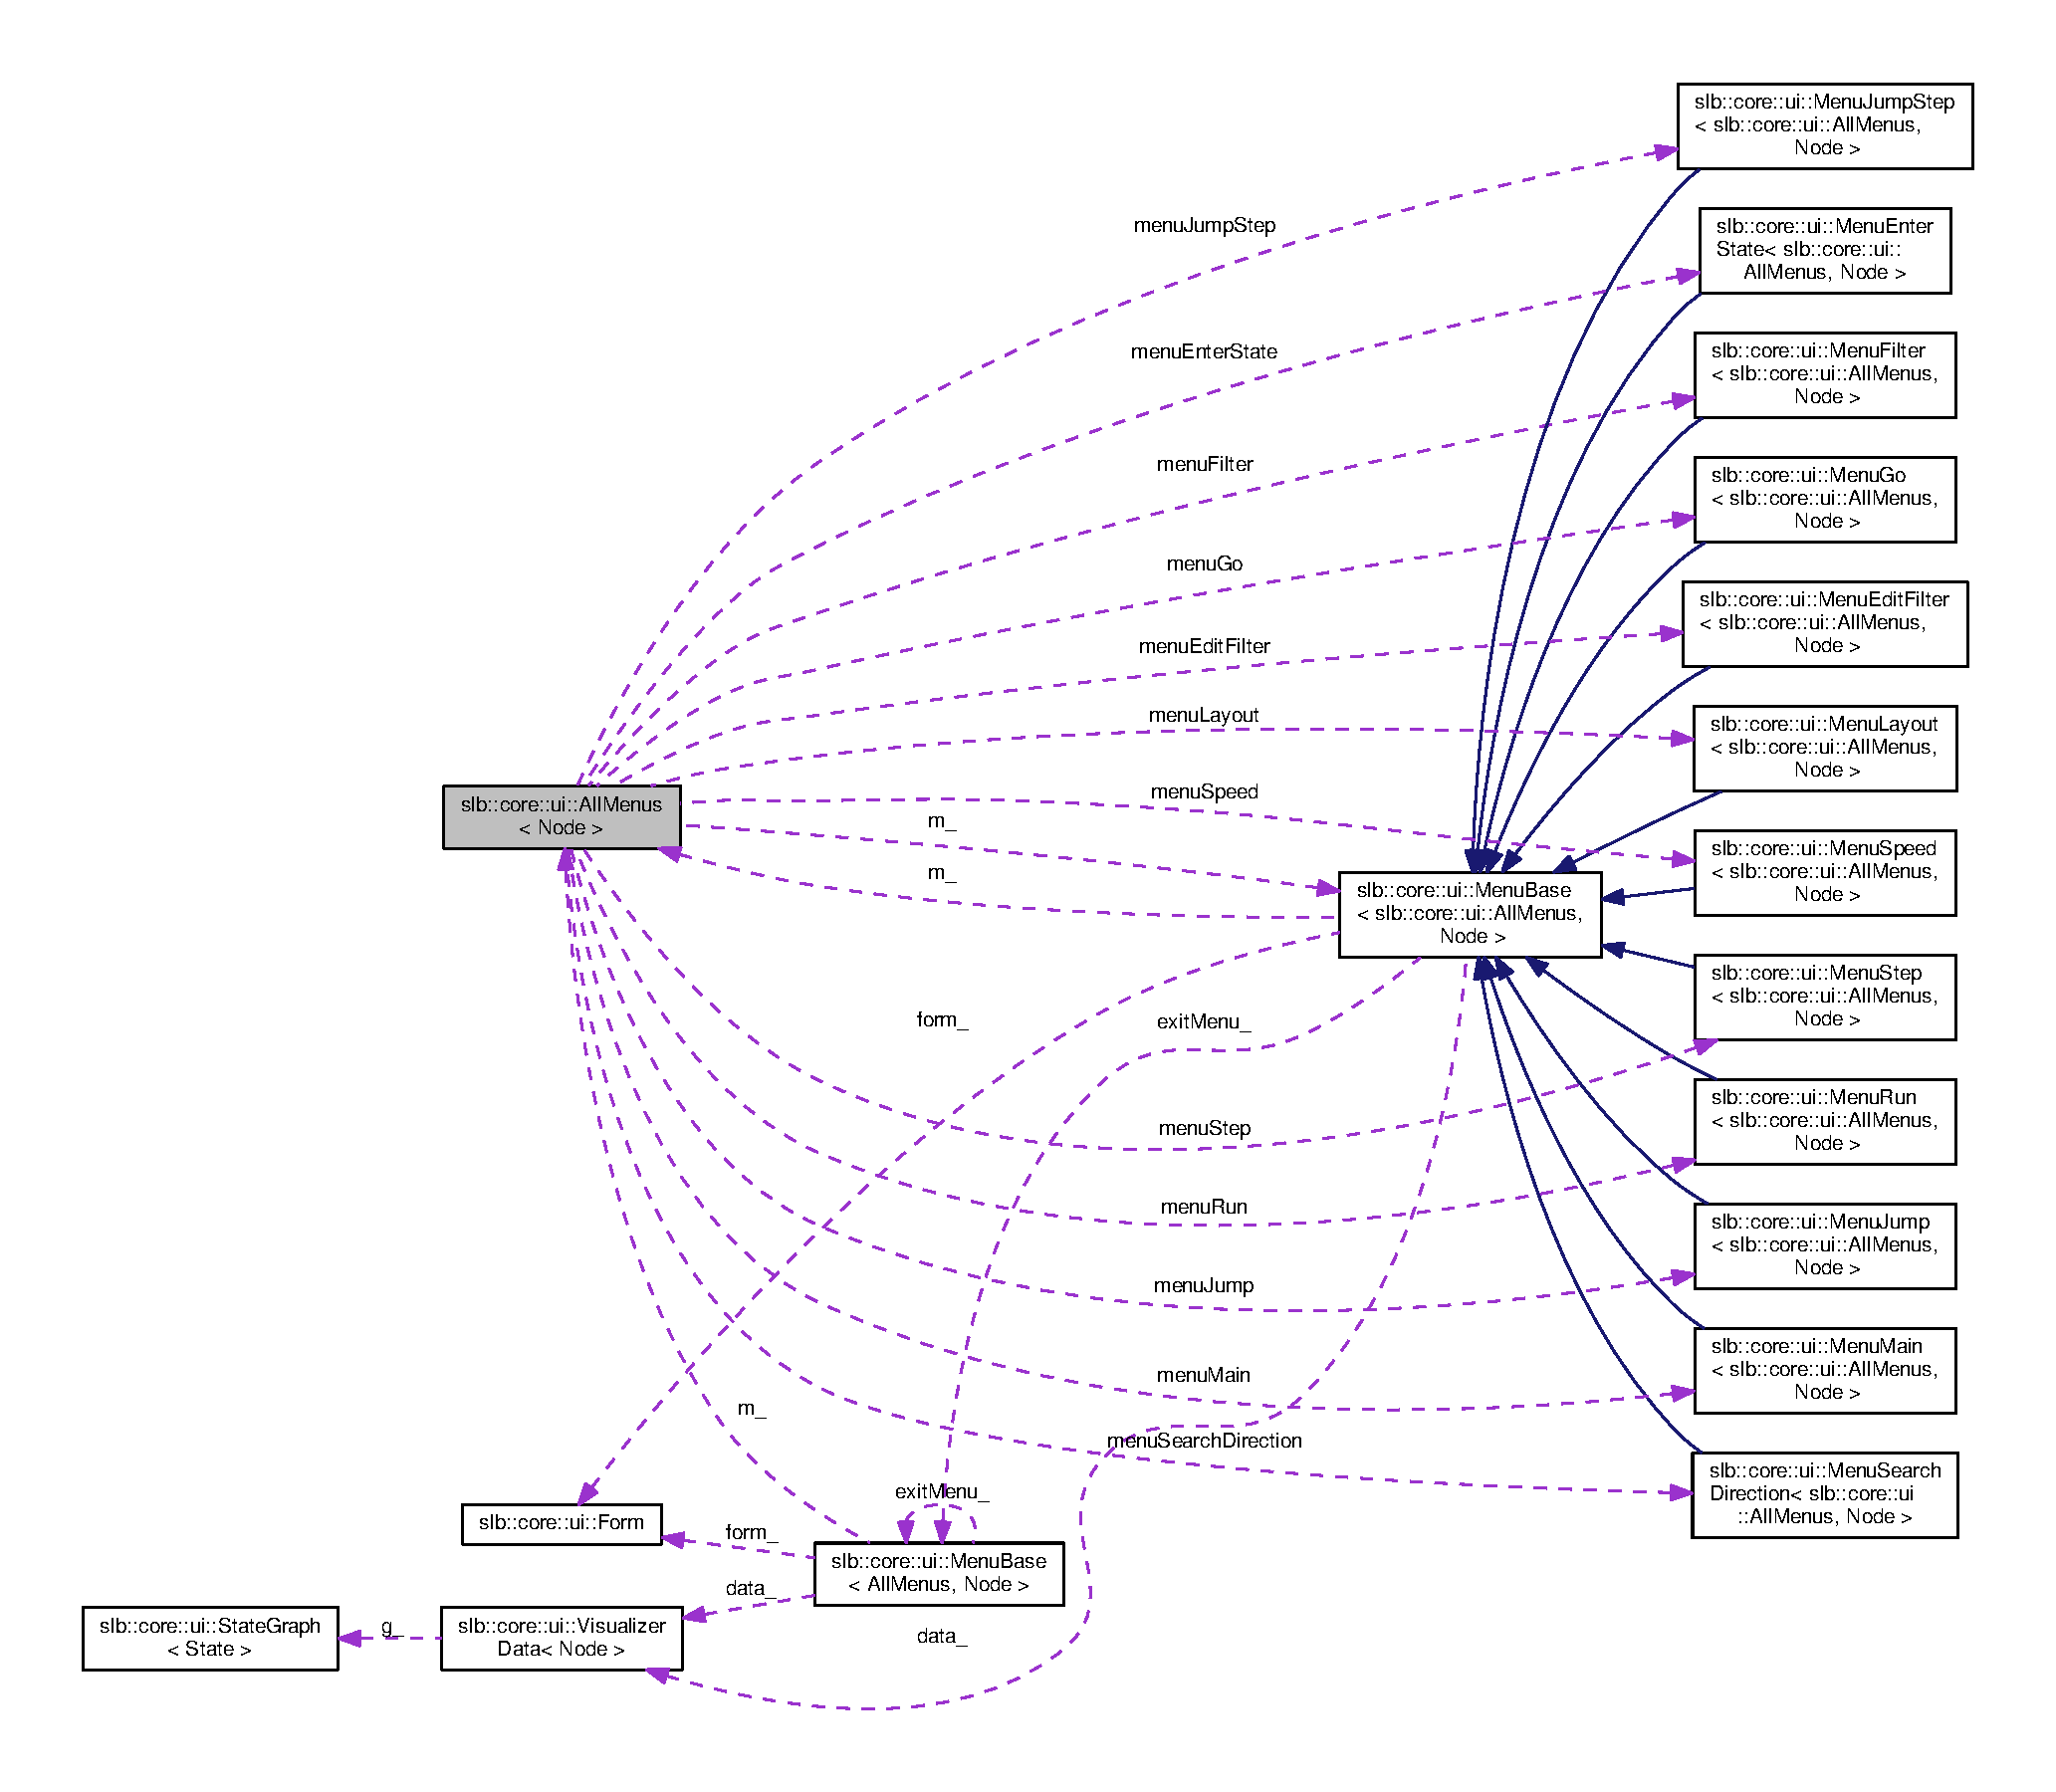
\includegraphics[width=350pt]{structslb_1_1core_1_1ui_1_1AllMenus__coll__graph}
\end{center}
\end{figure}
\subsubsection*{Public Member Functions}
\begin{DoxyCompactItemize}
\item 
\hyperlink{structslb_1_1core_1_1ui_1_1AllMenus_a0f13032d8c5a062c2dbb87b34d489ada}{All\+Menus} (\hyperlink{structslb_1_1core_1_1ui_1_1VisualizerData}{Visualizer\+Data}$<$ Node $>$ \&data)
\begin{DoxyCompactList}\small\item\em Initializes all the menus and sets the root menu as the current menu. \end{DoxyCompactList}\item 
\hyperlink{structslb_1_1core_1_1ui_1_1AllMenus_a0e46f55a2aac343cecd8a4b228126f47}{$\sim$\+All\+Menus} ()\hypertarget{structslb_1_1core_1_1ui_1_1AllMenus_a0e46f55a2aac343cecd8a4b228126f47}{}\label{structslb_1_1core_1_1ui_1_1AllMenus_a0e46f55a2aac343cecd8a4b228126f47}

\begin{DoxyCompactList}\small\item\em Destroys the current menu. \end{DoxyCompactList}\item 
void \hyperlink{structslb_1_1core_1_1ui_1_1AllMenus_a6deff049a64083c84141287f6f5679bd}{handle\+Enter} ()\hypertarget{structslb_1_1core_1_1ui_1_1AllMenus_a6deff049a64083c84141287f6f5679bd}{}\label{structslb_1_1core_1_1ui_1_1AllMenus_a6deff049a64083c84141287f6f5679bd}

\begin{DoxyCompactList}\small\item\em Handles the pressed Enter key by passing it to the handler of the currently active menu. \end{DoxyCompactList}\item 
void \hyperlink{structslb_1_1core_1_1ui_1_1AllMenus_af791972ca9bc24750ebd4b529fce6eea}{handle\+Esc} ()\hypertarget{structslb_1_1core_1_1ui_1_1AllMenus_af791972ca9bc24750ebd4b529fce6eea}{}\label{structslb_1_1core_1_1ui_1_1AllMenus_af791972ca9bc24750ebd4b529fce6eea}

\begin{DoxyCompactList}\small\item\em Handles the pressed Esc key by passing it to the handler of the currently active menu. \end{DoxyCompactList}\item 
void \hyperlink{structslb_1_1core_1_1ui_1_1AllMenus_a5cabf461bf71979f07a0f507e60baefe}{set\+Menu} (\hyperlink{structslb_1_1core_1_1ui_1_1MenuBase}{Menu\+Base}$<$ \hyperlink{structslb_1_1core_1_1ui_1_1AllMenus}{All\+Menus}, Node $>$ $\ast$new\+Menu, \hyperlink{structslb_1_1core_1_1ui_1_1LogWindow}{Log\+Window}$<$ Node $>$ \&log\+Window)
\begin{DoxyCompactList}\small\item\em Sets the new acive menu. The previously active menu is destroyed and the new active menu is created. This was the easiest way to reset things. \end{DoxyCompactList}\item 
\hyperlink{structslb_1_1core_1_1ui_1_1MenuBase}{Menu\+Base}$<$ \hyperlink{structslb_1_1core_1_1ui_1_1AllMenus}{All\+Menus}, Node $>$ $\ast$ \hyperlink{structslb_1_1core_1_1ui_1_1AllMenus_a84fab536b1f00eec48a3eaaf765fe27c}{cur\+Menu} ()
\begin{DoxyCompactList}\small\item\em Returns the currently active menu. \end{DoxyCompactList}\item 
\hyperlink{structslb_1_1core_1_1ui_1_1Form}{Form} \& \hyperlink{structslb_1_1core_1_1ui_1_1AllMenus_ad16885561afac21710be5effbaa0cb25}{cur\+Form} ()
\begin{DoxyCompactList}\small\item\em Returns the currently active form. \end{DoxyCompactList}\item 
M\+E\+NU $\ast$ \hyperlink{structslb_1_1core_1_1ui_1_1AllMenus_a059aff60e783f1c73783173327b81cf3}{raw} ()
\begin{DoxyCompactList}\small\item\em Returns the currently active menu in the raw {\ttfamily ncurses} format. \end{DoxyCompactList}\item 
std\+::vector$<$ I\+T\+EM $\ast$ $>$ \hyperlink{structslb_1_1core_1_1ui_1_1AllMenus_a531b3459a945dce28bbd8086d236be12}{menu\+Items} ()
\begin{DoxyCompactList}\small\item\em Returns the items of the active menu in the raw {\ttfamily ncurses} format. \end{DoxyCompactList}\end{DoxyCompactItemize}
\subsubsection*{Public Attributes}
\begin{DoxyCompactItemize}
\item 
bool \hyperlink{structslb_1_1core_1_1ui_1_1AllMenus_a7a65a1525bf95af856e2ebcaf238e09d}{hide\+Filtered} = true\hypertarget{structslb_1_1core_1_1ui_1_1AllMenus_a7a65a1525bf95af856e2ebcaf238e09d}{}\label{structslb_1_1core_1_1ui_1_1AllMenus_a7a65a1525bf95af856e2ebcaf238e09d}

\begin{DoxyCompactList}\small\item\em Indicates wither the filtered out events should be shown in the events pad of the log window. Always kept in sync with \hyperlink{structslb_1_1core_1_1ui_1_1LogWindow_a538ca4478f0ea842362b6754f8c80e22}{Log\+Window\+::hide\+Filtered\+\_\+}. \end{DoxyCompactList}\item 
bool \hyperlink{structslb_1_1core_1_1ui_1_1AllMenus_adbf624a1eba3c59852b5ed96cdfe80d3}{show\+Labels} = false\hypertarget{structslb_1_1core_1_1ui_1_1AllMenus_adbf624a1eba3c59852b5ed96cdfe80d3}{}\label{structslb_1_1core_1_1ui_1_1AllMenus_adbf624a1eba3c59852b5ed96cdfe80d3}

\begin{DoxyCompactList}\small\item\em Indicates wither the vertex and edge labels should be shown. Always kept in sync with \hyperlink{structslb_1_1core_1_1ui_1_1Drawer_a580db97e1c2261304eaa4dc63fb22c60}{Drawer\+::show\+Labels\+\_\+}. \end{DoxyCompactList}\item 
\hyperlink{structslb_1_1core_1_1ui_1_1MenuMain}{Menu\+Main}$<$ \hyperlink{structslb_1_1core_1_1ui_1_1AllMenus}{All\+Menus}, Node $>$ \hyperlink{structslb_1_1core_1_1ui_1_1AllMenus_ab7a574cb033c290bae6f39f43f6e08cd}{menu\+Main}\hypertarget{structslb_1_1core_1_1ui_1_1AllMenus_ab7a574cb033c290bae6f39f43f6e08cd}{}\label{structslb_1_1core_1_1ui_1_1AllMenus_ab7a574cb033c290bae6f39f43f6e08cd}

\begin{DoxyCompactList}\small\item\em The root menu. \end{DoxyCompactList}\item 
\hyperlink{structslb_1_1core_1_1ui_1_1MenuRun}{Menu\+Run}$<$ \hyperlink{structslb_1_1core_1_1ui_1_1AllMenus}{All\+Menus}, Node $>$ \hyperlink{structslb_1_1core_1_1ui_1_1AllMenus_af69fe9e838fdacf7a7f01c52f387d4a6}{menu\+Run}\hypertarget{structslb_1_1core_1_1ui_1_1AllMenus_af69fe9e838fdacf7a7f01c52f387d4a6}{}\label{structslb_1_1core_1_1ui_1_1AllMenus_af69fe9e838fdacf7a7f01c52f387d4a6}

\begin{DoxyCompactList}\small\item\em The menu reached when choosing the Run option from the root menu. \end{DoxyCompactList}\item 
\hyperlink{structslb_1_1core_1_1ui_1_1MenuEnterState}{Menu\+Enter\+State}$<$ \hyperlink{structslb_1_1core_1_1ui_1_1AllMenus}{All\+Menus}, Node $>$ \hyperlink{structslb_1_1core_1_1ui_1_1AllMenus_aaec00610ffe8e6dbd315d6ffbe956180}{menu\+Enter\+State}\hypertarget{structslb_1_1core_1_1ui_1_1AllMenus_aaec00610ffe8e6dbd315d6ffbe956180}{}\label{structslb_1_1core_1_1ui_1_1AllMenus_aaec00610ffe8e6dbd315d6ffbe956180}

\begin{DoxyCompactList}\small\item\em The menu reached when choosing the Search option from the root menu. \end{DoxyCompactList}\item 
\hyperlink{structslb_1_1core_1_1ui_1_1MenuFilter}{Menu\+Filter}$<$ \hyperlink{structslb_1_1core_1_1ui_1_1AllMenus}{All\+Menus}, Node $>$ \hyperlink{structslb_1_1core_1_1ui_1_1AllMenus_a3e154d2bfbc402ccc7d492de205aa6fe}{menu\+Filter}\hypertarget{structslb_1_1core_1_1ui_1_1AllMenus_a3e154d2bfbc402ccc7d492de205aa6fe}{}\label{structslb_1_1core_1_1ui_1_1AllMenus_a3e154d2bfbc402ccc7d492de205aa6fe}

\begin{DoxyCompactList}\small\item\em The menu reached when choosing the \hyperlink{structslb_1_1core_1_1ui_1_1Filter}{Filter} option from the root menu. \end{DoxyCompactList}\item 
\hyperlink{structslb_1_1core_1_1ui_1_1MenuGo}{Menu\+Go}$<$ \hyperlink{structslb_1_1core_1_1ui_1_1AllMenus}{All\+Menus}, Node $>$ \hyperlink{structslb_1_1core_1_1ui_1_1AllMenus_afb4250552b678cff7923b3bc57578bf4}{menu\+Go}\hypertarget{structslb_1_1core_1_1ui_1_1AllMenus_afb4250552b678cff7923b3bc57578bf4}{}\label{structslb_1_1core_1_1ui_1_1AllMenus_afb4250552b678cff7923b3bc57578bf4}

\begin{DoxyCompactList}\small\item\em The menu reached when choosing Run-\/$>$Go from the root menu. \end{DoxyCompactList}\item 
\hyperlink{structslb_1_1core_1_1ui_1_1MenuSpeed}{Menu\+Speed}$<$ \hyperlink{structslb_1_1core_1_1ui_1_1AllMenus}{All\+Menus}, Node $>$ \hyperlink{structslb_1_1core_1_1ui_1_1AllMenus_a353107b85b590f53dba00cf6bc73013f}{menu\+Speed}\hypertarget{structslb_1_1core_1_1ui_1_1AllMenus_a353107b85b590f53dba00cf6bc73013f}{}\label{structslb_1_1core_1_1ui_1_1AllMenus_a353107b85b590f53dba00cf6bc73013f}

\begin{DoxyCompactList}\small\item\em The menu reached when choosing Run-\/$>$Speed from the root menu. \end{DoxyCompactList}\item 
\hyperlink{structslb_1_1core_1_1ui_1_1MenuSearchDirection}{Menu\+Search\+Direction}$<$ \hyperlink{structslb_1_1core_1_1ui_1_1AllMenus}{All\+Menus}, Node $>$ \hyperlink{structslb_1_1core_1_1ui_1_1AllMenus_ac19791733540dbbbfa18b5c7a38a3e52}{menu\+Search\+Direction}\hypertarget{structslb_1_1core_1_1ui_1_1AllMenus_ac19791733540dbbbfa18b5c7a38a3e52}{}\label{structslb_1_1core_1_1ui_1_1AllMenus_ac19791733540dbbbfa18b5c7a38a3e52}

\begin{DoxyCompactList}\small\item\em The menu for choosing the search direction after specifying the search in the search menu (reached when choosing the Search option from the root menu). \end{DoxyCompactList}\item 
\hyperlink{structslb_1_1core_1_1ui_1_1MenuEditFilter}{Menu\+Edit\+Filter}$<$ \hyperlink{structslb_1_1core_1_1ui_1_1AllMenus}{All\+Menus}, Node $>$ \hyperlink{structslb_1_1core_1_1ui_1_1AllMenus_a64ce1352de888b4a963e1f1e52ddd770}{menu\+Edit\+Filter}\hypertarget{structslb_1_1core_1_1ui_1_1AllMenus_a64ce1352de888b4a963e1f1e52ddd770}{}\label{structslb_1_1core_1_1ui_1_1AllMenus_a64ce1352de888b4a963e1f1e52ddd770}

\begin{DoxyCompactList}\small\item\em The menu reached when choosing Filter-\/$>$Edit from the root menu. \end{DoxyCompactList}\item 
\hyperlink{structslb_1_1core_1_1ui_1_1MenuStep}{Menu\+Step}$<$ \hyperlink{structslb_1_1core_1_1ui_1_1AllMenus}{All\+Menus}, Node $>$ \hyperlink{structslb_1_1core_1_1ui_1_1AllMenus_a95a0884ed69014c8d7d4d79c70cd46b6}{menu\+Step}\hypertarget{structslb_1_1core_1_1ui_1_1AllMenus_a95a0884ed69014c8d7d4d79c70cd46b6}{}\label{structslb_1_1core_1_1ui_1_1AllMenus_a95a0884ed69014c8d7d4d79c70cd46b6}

\begin{DoxyCompactList}\small\item\em The menu reached when choosing Run-\/$>$Step from the root menu. \end{DoxyCompactList}\item 
\hyperlink{structslb_1_1core_1_1ui_1_1MenuJump}{Menu\+Jump}$<$ \hyperlink{structslb_1_1core_1_1ui_1_1AllMenus}{All\+Menus}, Node $>$ \hyperlink{structslb_1_1core_1_1ui_1_1AllMenus_a04f2d7f044dfc2267715f63eab5506f8}{menu\+Jump}\hypertarget{structslb_1_1core_1_1ui_1_1AllMenus_a04f2d7f044dfc2267715f63eab5506f8}{}\label{structslb_1_1core_1_1ui_1_1AllMenus_a04f2d7f044dfc2267715f63eab5506f8}

\begin{DoxyCompactList}\small\item\em The menu reached when choosing Run-\/$>$Jump from the root menu. \end{DoxyCompactList}\item 
\hyperlink{structslb_1_1core_1_1ui_1_1MenuJumpStep}{Menu\+Jump\+Step}$<$ \hyperlink{structslb_1_1core_1_1ui_1_1AllMenus}{All\+Menus}, Node $>$ \hyperlink{structslb_1_1core_1_1ui_1_1AllMenus_aa39e38f57bb86499ad1f507661bacad9}{menu\+Jump\+Step}\hypertarget{structslb_1_1core_1_1ui_1_1AllMenus_aa39e38f57bb86499ad1f507661bacad9}{}\label{structslb_1_1core_1_1ui_1_1AllMenus_aa39e38f57bb86499ad1f507661bacad9}

\begin{DoxyCompactList}\small\item\em The menu reached when choosing Run-\/$>$Jump-\/$>$Step from the root menu. \end{DoxyCompactList}\item 
\hyperlink{structslb_1_1core_1_1ui_1_1MenuLayout}{Menu\+Layout}$<$ \hyperlink{structslb_1_1core_1_1ui_1_1AllMenus}{All\+Menus}, Node $>$ \hyperlink{structslb_1_1core_1_1ui_1_1AllMenus_a8bde72e39ba430d5cc64c44b3f07c1c6}{menu\+Layout}\hypertarget{structslb_1_1core_1_1ui_1_1AllMenus_a8bde72e39ba430d5cc64c44b3f07c1c6}{}\label{structslb_1_1core_1_1ui_1_1AllMenus_a8bde72e39ba430d5cc64c44b3f07c1c6}

\begin{DoxyCompactList}\small\item\em The menu reached when choosing Run-\/$>$Layout from the root menu. \end{DoxyCompactList}\end{DoxyCompactItemize}
\subsubsection*{Private Attributes}
\begin{DoxyCompactItemize}
\item 
M\+E\+NU $\ast$ \hyperlink{structslb_1_1core_1_1ui_1_1AllMenus_ab6c6678fe02423faf7e86ebbb6e87b14}{raw\+\_\+} = nullptr\hypertarget{structslb_1_1core_1_1ui_1_1AllMenus_ab6c6678fe02423faf7e86ebbb6e87b14}{}\label{structslb_1_1core_1_1ui_1_1AllMenus_ab6c6678fe02423faf7e86ebbb6e87b14}

\begin{DoxyCompactList}\small\item\em The currently active menu in the raw {\ttfamily ncurses} format. \end{DoxyCompactList}\item 
\hyperlink{structslb_1_1core_1_1ui_1_1MenuBase}{Menu\+Base}$<$ \hyperlink{structslb_1_1core_1_1ui_1_1AllMenus}{All\+Menus}, Node $>$ $\ast$ \hyperlink{structslb_1_1core_1_1ui_1_1AllMenus_afa812ad21990179b69a1a74639fcebb6}{m\+\_\+} = nullptr\hypertarget{structslb_1_1core_1_1ui_1_1AllMenus_afa812ad21990179b69a1a74639fcebb6}{}\label{structslb_1_1core_1_1ui_1_1AllMenus_afa812ad21990179b69a1a74639fcebb6}

\begin{DoxyCompactList}\small\item\em The currently active menu. \end{DoxyCompactList}\item 
std\+::vector$<$ I\+T\+EM $\ast$ $>$ \hyperlink{structslb_1_1core_1_1ui_1_1AllMenus_ac85fb1060b5356bb5a56e6cfe6d3575c}{menu\+Items\+\_\+}\hypertarget{structslb_1_1core_1_1ui_1_1AllMenus_ac85fb1060b5356bb5a56e6cfe6d3575c}{}\label{structslb_1_1core_1_1ui_1_1AllMenus_ac85fb1060b5356bb5a56e6cfe6d3575c}

\begin{DoxyCompactList}\small\item\em Vector of pointers to items (in the raw {\ttfamily ncurses} format.) of the currently active menu. \end{DoxyCompactList}\item 
int \hyperlink{structslb_1_1core_1_1ui_1_1AllMenus_aad8ba60881528bf0fcea0ac85696e0ca}{max\+Menu\+Rows\+\_\+} = 3\hypertarget{structslb_1_1core_1_1ui_1_1AllMenus_aad8ba60881528bf0fcea0ac85696e0ca}{}\label{structslb_1_1core_1_1ui_1_1AllMenus_aad8ba60881528bf0fcea0ac85696e0ca}

\begin{DoxyCompactList}\small\item\em Max number of rows in the menu. \end{DoxyCompactList}\end{DoxyCompactItemize}


\subsubsection{Detailed Description}
\subsubsection*{template$<$class Node$>$\\*
struct slb\+::core\+::ui\+::\+All\+Menus$<$ Node $>$}

A holder for all the menus with an indicator of which menu and form are currently active. 


\begin{DoxyTemplParams}{Template Parameters}
{\em Node} & The search node type. \\
\hline
\end{DoxyTemplParams}


Definition at line 590 of file menus.\+h.



\subsubsection{Constructor \& Destructor Documentation}
\index{slb\+::core\+::ui\+::\+All\+Menus@{slb\+::core\+::ui\+::\+All\+Menus}!All\+Menus@{All\+Menus}}
\index{All\+Menus@{All\+Menus}!slb\+::core\+::ui\+::\+All\+Menus@{slb\+::core\+::ui\+::\+All\+Menus}}
\paragraph[{\texorpdfstring{All\+Menus(\+Visualizer\+Data$<$ Node $>$ \&data)}{AllMenus(VisualizerData< Node > &data)}}]{\setlength{\rightskip}{0pt plus 5cm}template$<$class Node$>$ {\bf slb\+::core\+::ui\+::\+All\+Menus}$<$ Node $>$\+::{\bf All\+Menus} (
\begin{DoxyParamCaption}
\item[{{\bf Visualizer\+Data}$<$ Node $>$ \&}]{data}
\end{DoxyParamCaption}
)\hspace{0.3cm}{\ttfamily [inline]}}\hypertarget{structslb_1_1core_1_1ui_1_1AllMenus_a0f13032d8c5a062c2dbb87b34d489ada}{}\label{structslb_1_1core_1_1ui_1_1AllMenus_a0f13032d8c5a062c2dbb87b34d489ada}


Initializes all the menus and sets the root menu as the current menu. 


\begin{DoxyParams}{Parameters}
{\em data} & reference to the constituent components of the visualizer. \\
\hline
\end{DoxyParams}


Definition at line 593 of file menus.\+h.



\subsubsection{Member Function Documentation}
\index{slb\+::core\+::ui\+::\+All\+Menus@{slb\+::core\+::ui\+::\+All\+Menus}!cur\+Form@{cur\+Form}}
\index{cur\+Form@{cur\+Form}!slb\+::core\+::ui\+::\+All\+Menus@{slb\+::core\+::ui\+::\+All\+Menus}}
\paragraph[{\texorpdfstring{cur\+Form()}{curForm()}}]{\setlength{\rightskip}{0pt plus 5cm}template$<$class Node$>$ {\bf Form}\& {\bf slb\+::core\+::ui\+::\+All\+Menus}$<$ Node $>$\+::cur\+Form (
\begin{DoxyParamCaption}
{}
\end{DoxyParamCaption}
)\hspace{0.3cm}{\ttfamily [inline]}}\hypertarget{structslb_1_1core_1_1ui_1_1AllMenus_ad16885561afac21710be5effbaa0cb25}{}\label{structslb_1_1core_1_1ui_1_1AllMenus_ad16885561afac21710be5effbaa0cb25}


Returns the currently active form. 

\begin{DoxyReturn}{Returns}
Reference to the currently active menu. 
\end{DoxyReturn}


Definition at line 685 of file menus.\+h.

\index{slb\+::core\+::ui\+::\+All\+Menus@{slb\+::core\+::ui\+::\+All\+Menus}!cur\+Menu@{cur\+Menu}}
\index{cur\+Menu@{cur\+Menu}!slb\+::core\+::ui\+::\+All\+Menus@{slb\+::core\+::ui\+::\+All\+Menus}}
\paragraph[{\texorpdfstring{cur\+Menu()}{curMenu()}}]{\setlength{\rightskip}{0pt plus 5cm}template$<$class Node$>$ {\bf Menu\+Base}$<${\bf All\+Menus}, Node$>$$\ast$ {\bf slb\+::core\+::ui\+::\+All\+Menus}$<$ Node $>$\+::cur\+Menu (
\begin{DoxyParamCaption}
{}
\end{DoxyParamCaption}
)\hspace{0.3cm}{\ttfamily [inline]}}\hypertarget{structslb_1_1core_1_1ui_1_1AllMenus_a84fab536b1f00eec48a3eaaf765fe27c}{}\label{structslb_1_1core_1_1ui_1_1AllMenus_a84fab536b1f00eec48a3eaaf765fe27c}


Returns the currently active menu. 

\begin{DoxyReturn}{Returns}
Pointer to the currently active menu. 
\end{DoxyReturn}


Definition at line 681 of file menus.\+h.

\index{slb\+::core\+::ui\+::\+All\+Menus@{slb\+::core\+::ui\+::\+All\+Menus}!menu\+Items@{menu\+Items}}
\index{menu\+Items@{menu\+Items}!slb\+::core\+::ui\+::\+All\+Menus@{slb\+::core\+::ui\+::\+All\+Menus}}
\paragraph[{\texorpdfstring{menu\+Items()}{menuItems()}}]{\setlength{\rightskip}{0pt plus 5cm}template$<$class Node$>$ std\+::vector$<$I\+T\+EM $\ast$$>$ {\bf slb\+::core\+::ui\+::\+All\+Menus}$<$ Node $>$\+::menu\+Items (
\begin{DoxyParamCaption}
{}
\end{DoxyParamCaption}
)\hspace{0.3cm}{\ttfamily [inline]}}\hypertarget{structslb_1_1core_1_1ui_1_1AllMenus_a531b3459a945dce28bbd8086d236be12}{}\label{structslb_1_1core_1_1ui_1_1AllMenus_a531b3459a945dce28bbd8086d236be12}


Returns the items of the active menu in the raw {\ttfamily ncurses} format. 

\begin{DoxyReturn}{Returns}
Vector of pointers to items (in the raw {\ttfamily ncurses} format.) of the currently active menu. 
\end{DoxyReturn}


Definition at line 695 of file menus.\+h.

\index{slb\+::core\+::ui\+::\+All\+Menus@{slb\+::core\+::ui\+::\+All\+Menus}!raw@{raw}}
\index{raw@{raw}!slb\+::core\+::ui\+::\+All\+Menus@{slb\+::core\+::ui\+::\+All\+Menus}}
\paragraph[{\texorpdfstring{raw()}{raw()}}]{\setlength{\rightskip}{0pt plus 5cm}template$<$class Node$>$ M\+E\+NU$\ast$ {\bf slb\+::core\+::ui\+::\+All\+Menus}$<$ Node $>$\+::raw (
\begin{DoxyParamCaption}
{}
\end{DoxyParamCaption}
)\hspace{0.3cm}{\ttfamily [inline]}}\hypertarget{structslb_1_1core_1_1ui_1_1AllMenus_a059aff60e783f1c73783173327b81cf3}{}\label{structslb_1_1core_1_1ui_1_1AllMenus_a059aff60e783f1c73783173327b81cf3}


Returns the currently active menu in the raw {\ttfamily ncurses} format. 

\begin{DoxyReturn}{Returns}
Pointer to the currently active menu in the raw {\ttfamily ncurses} format. 
\end{DoxyReturn}


Definition at line 690 of file menus.\+h.

\index{slb\+::core\+::ui\+::\+All\+Menus@{slb\+::core\+::ui\+::\+All\+Menus}!set\+Menu@{set\+Menu}}
\index{set\+Menu@{set\+Menu}!slb\+::core\+::ui\+::\+All\+Menus@{slb\+::core\+::ui\+::\+All\+Menus}}
\paragraph[{\texorpdfstring{set\+Menu(\+Menu\+Base$<$ All\+Menus, Node $>$ $\ast$new\+Menu, Log\+Window$<$ Node $>$ \&log\+Window)}{setMenu(MenuBase< AllMenus, Node > *newMenu, LogWindow< Node > &logWindow)}}]{\setlength{\rightskip}{0pt plus 5cm}template$<$class Node$>$ void {\bf slb\+::core\+::ui\+::\+All\+Menus}$<$ Node $>$\+::set\+Menu (
\begin{DoxyParamCaption}
\item[{{\bf Menu\+Base}$<$ {\bf All\+Menus}$<$ Node $>$, Node $>$ $\ast$}]{new\+Menu, }
\item[{{\bf Log\+Window}$<$ Node $>$ \&}]{log\+Window}
\end{DoxyParamCaption}
)\hspace{0.3cm}{\ttfamily [inline]}}\hypertarget{structslb_1_1core_1_1ui_1_1AllMenus_a5cabf461bf71979f07a0f507e60baefe}{}\label{structslb_1_1core_1_1ui_1_1AllMenus_a5cabf461bf71979f07a0f507e60baefe}


Sets the new acive menu. The previously active menu is destroyed and the new active menu is created. This was the easiest way to reset things. 


\begin{DoxyParams}{Parameters}
{\em new\+Menu} & The newly active menu. \\
\hline
{\em log\+Window} & Reference to the log window. \\
\hline
\end{DoxyParams}


Definition at line 665 of file menus.\+h.



The documentation for this struct was generated from the following file\+:\begin{DoxyCompactItemize}
\item 
core/user\+\_\+interface/\hyperlink{menus_8h}{menus.\+h}\end{DoxyCompactItemize}

\hypertarget{structslb_1_1ext_1_1algorithm_1_1Astar}{}\subsection{slb\+:\+:ext\+:\+:algorithm\+:\+:Astar$<$ A\+L\+G\+\_\+\+T\+P\+A\+R\+A\+MS, Open\+\_\+ $>$ Struct Template Reference}
\label{structslb_1_1ext_1_1algorithm_1_1Astar}\index{slb\+::ext\+::algorithm\+::\+Astar$<$ A\+L\+G\+\_\+\+T\+P\+A\+R\+A\+M\+S, Open\+\_\+ $>$@{slb\+::ext\+::algorithm\+::\+Astar$<$ A\+L\+G\+\_\+\+T\+P\+A\+R\+A\+M\+S, Open\+\_\+ $>$}}


The {\ttfamily A$\ast$} search algorithm.  




{\ttfamily \#include $<$astar.\+h$>$}



Inheritance diagram for slb\+:\+:ext\+:\+:algorithm\+:\+:Astar$<$ A\+L\+G\+\_\+\+T\+P\+A\+R\+A\+MS, Open\+\_\+ $>$\+:\nopagebreak
\begin{figure}[H]
\begin{center}
\leavevmode
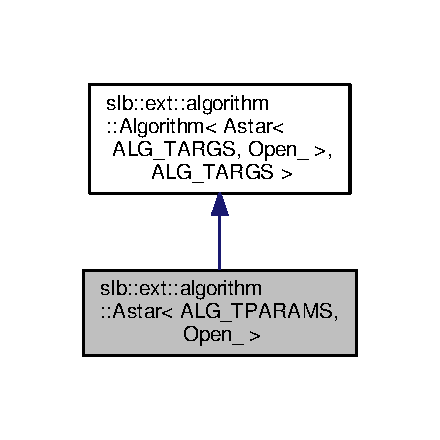
\includegraphics[width=211pt]{structslb_1_1ext_1_1algorithm_1_1Astar__inherit__graph}
\end{center}
\end{figure}


Collaboration diagram for slb\+:\+:ext\+:\+:algorithm\+:\+:Astar$<$ A\+L\+G\+\_\+\+T\+P\+A\+R\+A\+MS, Open\+\_\+ $>$\+:\nopagebreak
\begin{figure}[H]
\begin{center}
\leavevmode
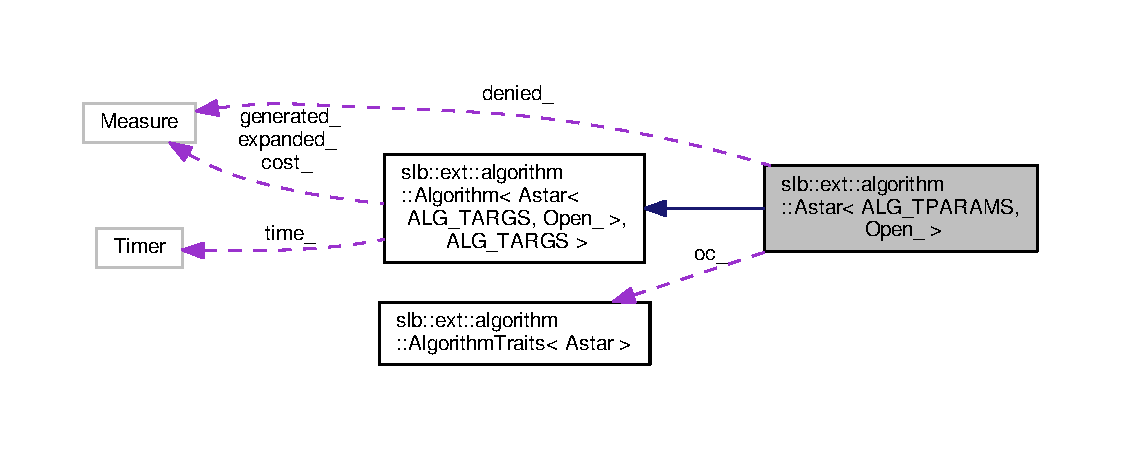
\includegraphics[width=350pt]{structslb_1_1ext_1_1algorithm_1_1Astar__coll__graph}
\end{center}
\end{figure}
\subsubsection*{Public Types}
\begin{DoxyCompactItemize}
\item 
using \hyperlink{structslb_1_1ext_1_1algorithm_1_1Astar_a007033a41137be7d62861e1b10c204d9}{Open} = Open\+\_\+$<$ \hyperlink{structslb_1_1ext_1_1algorithm_1_1Astar}{Astar} $>$\hypertarget{structslb_1_1ext_1_1algorithm_1_1Astar_a007033a41137be7d62861e1b10c204d9}{}\label{structslb_1_1ext_1_1algorithm_1_1Astar_a007033a41137be7d62861e1b10c204d9}

\begin{DoxyCompactList}\small\item\em The open list type. \end{DoxyCompactList}\item 
using \hyperlink{structslb_1_1ext_1_1algorithm_1_1Astar_a7c221266394f6833a6f5aadb0f76315d}{OC} = typename \hyperlink{classslb_1_1ext_1_1algorithm_1_1AlgorithmTraits}{Algorithm\+Traits}$<$ \hyperlink{structslb_1_1ext_1_1algorithm_1_1Astar}{Astar} $>$\+::\hyperlink{structslb_1_1ext_1_1algorithm_1_1Astar_a7c221266394f6833a6f5aadb0f76315d}{OC}\hypertarget{structslb_1_1ext_1_1algorithm_1_1Astar_a7c221266394f6833a6f5aadb0f76315d}{}\label{structslb_1_1ext_1_1algorithm_1_1Astar_a7c221266394f6833a6f5aadb0f76315d}

\begin{DoxyCompactList}\small\item\em Open\+Closed list type. \end{DoxyCompactList}\item 
using \hyperlink{structslb_1_1ext_1_1algorithm_1_1Astar_a1c38f30602110360ceb99e12b055432f}{Neighbor} = typename \hyperlink{classslb_1_1ext_1_1algorithm_1_1AlgorithmTraits}{Algorithm\+Traits}$<$ \hyperlink{structslb_1_1ext_1_1algorithm_1_1Astar}{Astar} $>$\+::Generator\+::\+Neighbor\hypertarget{structslb_1_1ext_1_1algorithm_1_1Astar_a1c38f30602110360ceb99e12b055432f}{}\label{structslb_1_1ext_1_1algorithm_1_1Astar_a1c38f30602110360ceb99e12b055432f}

\begin{DoxyCompactList}\small\item\em Search neighbor type. \end{DoxyCompactList}\item 
using \hyperlink{structslb_1_1ext_1_1algorithm_1_1Astar_ae3dc41bb8fd97c3669db3704b24f2a1f}{Direct\+Base} = \hyperlink{structslb_1_1ext_1_1algorithm_1_1Algorithm}{Algorithm}$<$ \hyperlink{structslb_1_1ext_1_1algorithm_1_1Astar}{Astar}$<$ \hyperlink{algorithm_8h_a425b5a86fe8dae889a8343e14267c3c0}{A\+L\+G\+\_\+\+T\+A\+R\+GS}, Open\+\_\+ $>$, \hyperlink{algorithm_8h_a425b5a86fe8dae889a8343e14267c3c0}{A\+L\+G\+\_\+\+T\+A\+R\+GS} $>$\hypertarget{structslb_1_1ext_1_1algorithm_1_1Astar_ae3dc41bb8fd97c3669db3704b24f2a1f}{}\label{structslb_1_1ext_1_1algorithm_1_1Astar_ae3dc41bb8fd97c3669db3704b24f2a1f}

\begin{DoxyCompactList}\small\item\em The direct base. \end{DoxyCompactList}\item 
using \hyperlink{structslb_1_1ext_1_1algorithm_1_1Astar_a44bf47362f5c203a2a637c986da15f47}{Goal\+Handler} = typename \hyperlink{structslb_1_1ext_1_1algorithm_1_1Algorithm_ae0c6a75028107e4642e43798f21f4bfc}{Direct\+Base\+::\+Goal\+Handler}\hypertarget{structslb_1_1ext_1_1algorithm_1_1Astar_a44bf47362f5c203a2a637c986da15f47}{}\label{structslb_1_1ext_1_1algorithm_1_1Astar_a44bf47362f5c203a2a637c986da15f47}

\begin{DoxyCompactList}\small\item\em The goal handler policy. \end{DoxyCompactList}\item 
using \hyperlink{structslb_1_1ext_1_1algorithm_1_1Astar_a0d23cb786a79d57e4319e62bc6427d16}{Initial\+Heuristic} = typename \hyperlink{structslb_1_1ext_1_1algorithm_1_1Algorithm_ad1f8f28e7b07f747ef7b7b5bf0643c2d}{Direct\+Base\+::\+Initial\+Heuristic}\hypertarget{structslb_1_1ext_1_1algorithm_1_1Astar_a0d23cb786a79d57e4319e62bc6427d16}{}\label{structslb_1_1ext_1_1algorithm_1_1Astar_a0d23cb786a79d57e4319e62bc6427d16}

\begin{DoxyCompactList}\small\item\em The initial heuristic policy. \end{DoxyCompactList}\item 
using \hyperlink{structslb_1_1ext_1_1algorithm_1_1Astar_a8e7c4ac827051423153a315c7b404119}{Generator} = typename \hyperlink{structslb_1_1ext_1_1algorithm_1_1Algorithm_afa5a78c048b4fe4f5848aeaf5c1f8d65}{Direct\+Base\+::\+Generator}\hypertarget{structslb_1_1ext_1_1algorithm_1_1Astar_a8e7c4ac827051423153a315c7b404119}{}\label{structslb_1_1ext_1_1algorithm_1_1Astar_a8e7c4ac827051423153a315c7b404119}

\begin{DoxyCompactList}\small\item\em The generator policy. \end{DoxyCompactList}\item 
using \hyperlink{structslb_1_1ext_1_1algorithm_1_1Astar_a49c5252e4f03e05f60409d22beaf4c8e}{My\+Type} = \hyperlink{structslb_1_1ext_1_1algorithm_1_1Astar}{Astar}\hypertarget{structslb_1_1ext_1_1algorithm_1_1Astar_a49c5252e4f03e05f60409d22beaf4c8e}{}\label{structslb_1_1ext_1_1algorithm_1_1Astar_a49c5252e4f03e05f60409d22beaf4c8e}

\begin{DoxyCompactList}\small\item\em The type of \hyperlink{structslb_1_1ext_1_1algorithm_1_1Astar}{Astar}; required for \hyperlink{algorithm_8h_a64c012078deee9a30405e18ec11e6360}{A\+L\+G\+\_\+\+D\+A\+TA} symbol. \end{DoxyCompactList}\item 
using {\bfseries Distance\+Map} = std\+::unordered\+\_\+map$<$ State, Cost\+Type, \hyperlink{structslb_1_1core_1_1util_1_1StateHash}{core\+::util\+::\+State\+Hash}$<$ State $>$$>$\hypertarget{structslb_1_1ext_1_1algorithm_1_1Astar_a210d1f8bc1c2e97e626deb1051de2b2b}{}\label{structslb_1_1ext_1_1algorithm_1_1Astar_a210d1f8bc1c2e97e626deb1051de2b2b}

\end{DoxyCompactItemize}
\subsubsection*{Public Member Functions}
\begin{DoxyCompactItemize}
\item 
\hyperlink{structslb_1_1ext_1_1algorithm_1_1Astar_a2d3050a9cc4dddc9f48b7c42d11d68c9}{Astar} (const My\+Instance \&instance)
\begin{DoxyCompactList}\small\item\em Initializes the algorithm based on the problem instance. \end{DoxyCompactList}\item 
Return\+Type \hyperlink{structslb_1_1ext_1_1algorithm_1_1Astar_af46d0fe401539d7ae297dc4d059f5b5f}{run} ()
\begin{DoxyCompactList}\small\item\em Runs the algorithm. \end{DoxyCompactList}\item 
\hyperlink{structslb_1_1core_1_1sb_1_1MeasureSet}{Measure\+Set} \hyperlink{structslb_1_1ext_1_1algorithm_1_1Astar_a936b71c860389ebadb17ee8afaba875f}{measures} () const 
\begin{DoxyCompactList}\small\item\em Returns the statistics about the search algorithm\textquotesingle{}s performance for solving the particular instance. \end{DoxyCompactList}\item 
\hyperlink{structslb_1_1core_1_1ui_1_1StateGraph}{core\+::ui\+::\+State\+Graph}$<$ State $>$ \hyperlink{structslb_1_1ext_1_1algorithm_1_1Astar_a15d6101b6dc84cb71e290c3fcdcb44b9}{graph} () const 
\begin{DoxyCompactList}\small\item\em Computes the state graph based on the closed list. \end{DoxyCompactList}\item 
Cost\+Type \hyperlink{structslb_1_1ext_1_1algorithm_1_1Astar_a67abf0fa88aebf52c644731701a0dd70}{distance} (const State \&s)
\begin{DoxyCompactList}\small\item\em Computes the distance to the given state. Returns Cost\+Type\{-\/1\} if that distance has not been computed. \end{DoxyCompactList}\item 
Distance\+Map \hyperlink{structslb_1_1ext_1_1algorithm_1_1Astar_a2c129f68cc11d10fefa4fa40d58ba6a2}{distance\+Map} () const 
\begin{DoxyCompactList}\small\item\em Computes the distance map based on the current state of the closed list. \end{DoxyCompactList}\end{DoxyCompactItemize}
\begin{Indent}{\bf Services for policies.}\par
\begin{DoxyCompactItemize}
\item 
\hyperlink{structslb_1_1ext_1_1algorithm_1_1Astar_a7c221266394f6833a6f5aadb0f76315d}{OC} \& {\bfseries oc} ()\hypertarget{structslb_1_1ext_1_1algorithm_1_1Astar_a60959a673f2908ca3cd8dd864b486e64}{}\label{structslb_1_1ext_1_1algorithm_1_1Astar_a60959a673f2908ca3cd8dd864b486e64}

\item 
Node $\ast$ {\bfseries cur} ()\hypertarget{structslb_1_1ext_1_1algorithm_1_1Astar_ac650497d106eb9328f2cbdf0b25bb35f}{}\label{structslb_1_1ext_1_1algorithm_1_1Astar_ac650497d106eb9328f2cbdf0b25bb35f}

\item 
Measure \& {\bfseries denied} ()\hypertarget{structslb_1_1ext_1_1algorithm_1_1Astar_a9eb913b6ba31da6179009bcf23a4c551}{}\label{structslb_1_1ext_1_1algorithm_1_1Astar_a9eb913b6ba31da6179009bcf23a4c551}

\item 
void {\bfseries recompute\+Open} ()\hypertarget{structslb_1_1ext_1_1algorithm_1_1Astar_a52da702a953cda53a341c1a9ab0d701a}{}\label{structslb_1_1ext_1_1algorithm_1_1Astar_a52da702a953cda53a341c1a9ab0d701a}

\item 
{\footnotesize template$<$typename P $>$ }\\void {\bfseries partial\+Recompute\+Open} (const P \&p)\hypertarget{structslb_1_1ext_1_1algorithm_1_1Astar_a89bd403817a1192686aeb5fd85047a3a}{}\label{structslb_1_1ext_1_1algorithm_1_1Astar_a89bd403817a1192686aeb5fd85047a3a}

\end{DoxyCompactItemize}
\end{Indent}
\subsubsection*{Private Member Functions}
\begin{DoxyCompactItemize}
\item 
void \hyperlink{structslb_1_1ext_1_1algorithm_1_1Astar_a3174abc49367f3f0ac6c4da24c5023a6}{handle\+Selected} ()\hypertarget{structslb_1_1ext_1_1algorithm_1_1Astar_a3174abc49367f3f0ac6c4da24c5023a6}{}\label{structslb_1_1ext_1_1algorithm_1_1Astar_a3174abc49367f3f0ac6c4da24c5023a6}

\begin{DoxyCompactList}\small\item\em Handles the selected node. \end{DoxyCompactList}\item 
void \hyperlink{structslb_1_1ext_1_1algorithm_1_1Astar_a48ea2eb2a9199b063c8511e9eb5521c1}{handle\+Selected} (std\+::true\+\_\+type)\hypertarget{structslb_1_1ext_1_1algorithm_1_1Astar_a48ea2eb2a9199b063c8511e9eb5521c1}{}\label{structslb_1_1ext_1_1algorithm_1_1Astar_a48ea2eb2a9199b063c8511e9eb5521c1}

\begin{DoxyCompactList}\small\item\em Handles the selected node in the case that suspensions are to be dealt with. \end{DoxyCompactList}\item 
void \hyperlink{structslb_1_1ext_1_1algorithm_1_1Astar_a82f96441870d908bbb75bed33bfc1ff0}{handle\+Selected} (std\+::false\+\_\+type)\hypertarget{structslb_1_1ext_1_1algorithm_1_1Astar_a82f96441870d908bbb75bed33bfc1ff0}{}\label{structslb_1_1ext_1_1algorithm_1_1Astar_a82f96441870d908bbb75bed33bfc1ff0}

\begin{DoxyCompactList}\small\item\em Handles the selected node in the case that suspensions do not need to be dealt with. \end{DoxyCompactList}\item 
void \hyperlink{structslb_1_1ext_1_1algorithm_1_1Astar_a8aca907e8697bde36dd3889bcf13e6cd}{expand} ()\hypertarget{structslb_1_1ext_1_1algorithm_1_1Astar_a8aca907e8697bde36dd3889bcf13e6cd}{}\label{structslb_1_1ext_1_1algorithm_1_1Astar_a8aca907e8697bde36dd3889bcf13e6cd}

\begin{DoxyCompactList}\small\item\em Expands the selected node. \end{DoxyCompactList}\item 
void \hyperlink{structslb_1_1ext_1_1algorithm_1_1Astar_a32a1daf8bb9e1686c38182125c647bcb}{handle\+Neighbor} (\hyperlink{structslb_1_1ext_1_1algorithm_1_1Astar_a1c38f30602110360ceb99e12b055432f}{Neighbor} \&n)
\begin{DoxyCompactList}\small\item\em Handles the current neighbor. \end{DoxyCompactList}\end{DoxyCompactItemize}
\subsubsection*{Private Attributes}
\begin{DoxyCompactItemize}
\item 
\hyperlink{structslb_1_1ext_1_1algorithm_1_1Astar_a7c221266394f6833a6f5aadb0f76315d}{OC} \hyperlink{structslb_1_1ext_1_1algorithm_1_1Astar_a67914aa334ddbb3530ffc21190709e5d}{oc\+\_\+}\hypertarget{structslb_1_1ext_1_1algorithm_1_1Astar_a67914aa334ddbb3530ffc21190709e5d}{}\label{structslb_1_1ext_1_1algorithm_1_1Astar_a67914aa334ddbb3530ffc21190709e5d}

\begin{DoxyCompactList}\small\item\em The open and closed lists. \end{DoxyCompactList}\item 
Node $\ast$ \hyperlink{structslb_1_1ext_1_1algorithm_1_1Astar_a92032cb21d6d47bb3c66b3e261220b93}{cur\+\_\+}\hypertarget{structslb_1_1ext_1_1algorithm_1_1Astar_a92032cb21d6d47bb3c66b3e261220b93}{}\label{structslb_1_1ext_1_1algorithm_1_1Astar_a92032cb21d6d47bb3c66b3e261220b93}

\begin{DoxyCompactList}\small\item\em The currently selected node. \end{DoxyCompactList}\item 
Measure \hyperlink{structslb_1_1ext_1_1algorithm_1_1Astar_a205d1811287b6fe7f7d8f19b37b0f667}{denied\+\_\+} \{\char`\"{}Denied\char`\"{}\}\hypertarget{structslb_1_1ext_1_1algorithm_1_1Astar_a205d1811287b6fe7f7d8f19b37b0f667}{}\label{structslb_1_1ext_1_1algorithm_1_1Astar_a205d1811287b6fe7f7d8f19b37b0f667}

\begin{DoxyCompactList}\small\item\em The number of denied expansions. \end{DoxyCompactList}\end{DoxyCompactItemize}
\subsubsection*{Additional Inherited Members}


\subsubsection{Detailed Description}
\subsubsection*{template$<$A\+L\+G\+\_\+\+T\+P\+A\+R\+A\+MS, template$<$ class $>$ class Open\+\_\+ = S\+L\+B\+\_\+\+OL$>$\\*
struct slb\+::ext\+::algorithm\+::\+Astar$<$ A\+L\+G\+\_\+\+T\+P\+A\+R\+A\+M\+S, Open\+\_\+ $>$}

The {\ttfamily A$\ast$} search algorithm. 


\begin{DoxyTemplParams}{Template Parameters}
{\em log\+Flag} & If {\ttfamily true}, the events generated by the search algorithm are logged. Otherwise, they are not. \\
\hline
{\em Node\+\_\+} & The search node type. \\
\hline
{\em Goal\+Handler} & The policy for handling goal conditions. \\
\hline
{\em Initial\+Heuristic} & The initial heuristic used by the search algorithm. \\
\hline
{\em Open} & The open list type. \\
\hline
\end{DoxyTemplParams}
\begin{DoxyNote}{Note}
See the documentation for \hyperlink{algorithm_8h_a521ad67aee0e10fb76ee132a9d5c0768}{A\+L\+G\+\_\+\+T\+P\+A\+R\+A\+MS} and \hyperlink{algorithm_8h_a64c012078deee9a30405e18ec11e6360}{A\+L\+G\+\_\+\+D\+A\+TA}. 
\end{DoxyNote}


Definition at line 15 of file astar.\+h.



\subsubsection{Constructor \& Destructor Documentation}
\index{slb\+::ext\+::algorithm\+::\+Astar@{slb\+::ext\+::algorithm\+::\+Astar}!Astar@{Astar}}
\index{Astar@{Astar}!slb\+::ext\+::algorithm\+::\+Astar@{slb\+::ext\+::algorithm\+::\+Astar}}
\paragraph[{\texorpdfstring{Astar(const My\+Instance \&instance)}{Astar(const MyInstance &instance)}}]{\setlength{\rightskip}{0pt plus 5cm}template$<$A\+L\+G\+\_\+\+T\+P\+A\+R\+A\+MS , template$<$ class $>$ class Open\+\_\+ = S\+L\+B\+\_\+\+OL$>$ {\bf slb\+::ext\+::algorithm\+::\+Astar}$<$ {\bf A\+L\+G\+\_\+\+T\+P\+A\+R\+A\+MS}, Open\+\_\+ $>$\+::{\bf Astar} (
\begin{DoxyParamCaption}
\item[{const My\+Instance \&}]{instance}
\end{DoxyParamCaption}
)\hspace{0.3cm}{\ttfamily [inline]}}\hypertarget{structslb_1_1ext_1_1algorithm_1_1Astar_a2d3050a9cc4dddc9f48b7c42d11d68c9}{}\label{structslb_1_1ext_1_1algorithm_1_1Astar_a2d3050a9cc4dddc9f48b7c42d11d68c9}


Initializes the algorithm based on the problem instance. 


\begin{DoxyParams}{Parameters}
{\em instance} & The problem instance. \\
\hline
\end{DoxyParams}


Definition at line 76 of file astar.\+h.



\subsubsection{Member Function Documentation}
\index{slb\+::ext\+::algorithm\+::\+Astar@{slb\+::ext\+::algorithm\+::\+Astar}!distance@{distance}}
\index{distance@{distance}!slb\+::ext\+::algorithm\+::\+Astar@{slb\+::ext\+::algorithm\+::\+Astar}}
\paragraph[{\texorpdfstring{distance(const State \&s)}{distance(const State &s)}}]{\setlength{\rightskip}{0pt plus 5cm}template$<$A\+L\+G\+\_\+\+T\+P\+A\+R\+A\+MS , template$<$ class $>$ class Open\+\_\+ = S\+L\+B\+\_\+\+OL$>$ Cost\+Type {\bf slb\+::ext\+::algorithm\+::\+Astar}$<$ {\bf A\+L\+G\+\_\+\+T\+P\+A\+R\+A\+MS}, Open\+\_\+ $>$\+::distance (
\begin{DoxyParamCaption}
\item[{const State \&}]{s}
\end{DoxyParamCaption}
)\hspace{0.3cm}{\ttfamily [inline]}}\hypertarget{structslb_1_1ext_1_1algorithm_1_1Astar_a67abf0fa88aebf52c644731701a0dd70}{}\label{structslb_1_1ext_1_1algorithm_1_1Astar_a67abf0fa88aebf52c644731701a0dd70}


Computes the distance to the given state. Returns Cost\+Type\{-\/1\} if that distance has not been computed. 


\begin{DoxyParams}{Parameters}
{\em s} & The state. \\
\hline
\end{DoxyParams}
\begin{DoxyReturn}{Returns}
The distance to {\ttfamily s}. 
\end{DoxyReturn}


Definition at line 132 of file astar.\+h.

\index{slb\+::ext\+::algorithm\+::\+Astar@{slb\+::ext\+::algorithm\+::\+Astar}!distance\+Map@{distance\+Map}}
\index{distance\+Map@{distance\+Map}!slb\+::ext\+::algorithm\+::\+Astar@{slb\+::ext\+::algorithm\+::\+Astar}}
\paragraph[{\texorpdfstring{distance\+Map() const }{distanceMap() const }}]{\setlength{\rightskip}{0pt plus 5cm}template$<$A\+L\+G\+\_\+\+T\+P\+A\+R\+A\+MS , template$<$ class $>$ class Open\+\_\+ = S\+L\+B\+\_\+\+OL$>$ Distance\+Map {\bf slb\+::ext\+::algorithm\+::\+Astar}$<$ {\bf A\+L\+G\+\_\+\+T\+P\+A\+R\+A\+MS}, Open\+\_\+ $>$\+::distance\+Map (
\begin{DoxyParamCaption}
{}
\end{DoxyParamCaption}
) const\hspace{0.3cm}{\ttfamily [inline]}}\hypertarget{structslb_1_1ext_1_1algorithm_1_1Astar_a2c129f68cc11d10fefa4fa40d58ba6a2}{}\label{structslb_1_1ext_1_1algorithm_1_1Astar_a2c129f68cc11d10fefa4fa40d58ba6a2}


Computes the distance map based on the current state of the closed list. 

\begin{DoxyReturn}{Returns}
The distance map based on the current state of the closed list. 
\end{DoxyReturn}


Definition at line 140 of file astar.\+h.

\index{slb\+::ext\+::algorithm\+::\+Astar@{slb\+::ext\+::algorithm\+::\+Astar}!graph@{graph}}
\index{graph@{graph}!slb\+::ext\+::algorithm\+::\+Astar@{slb\+::ext\+::algorithm\+::\+Astar}}
\paragraph[{\texorpdfstring{graph() const }{graph() const }}]{\setlength{\rightskip}{0pt plus 5cm}template$<$A\+L\+G\+\_\+\+T\+P\+A\+R\+A\+MS , template$<$ class $>$ class Open\+\_\+ = S\+L\+B\+\_\+\+OL$>$ {\bf core\+::ui\+::\+State\+Graph}$<$State$>$ {\bf slb\+::ext\+::algorithm\+::\+Astar}$<$ {\bf A\+L\+G\+\_\+\+T\+P\+A\+R\+A\+MS}, Open\+\_\+ $>$\+::graph (
\begin{DoxyParamCaption}
{}
\end{DoxyParamCaption}
) const\hspace{0.3cm}{\ttfamily [inline]}}\hypertarget{structslb_1_1ext_1_1algorithm_1_1Astar_a15d6101b6dc84cb71e290c3fcdcb44b9}{}\label{structslb_1_1ext_1_1algorithm_1_1Astar_a15d6101b6dc84cb71e290c3fcdcb44b9}


Computes the state graph based on the closed list. 

\begin{DoxyReturn}{Returns}
The state graph computed based on the closed list. 
\end{DoxyReturn}


Definition at line 112 of file astar.\+h.

\index{slb\+::ext\+::algorithm\+::\+Astar@{slb\+::ext\+::algorithm\+::\+Astar}!handle\+Neighbor@{handle\+Neighbor}}
\index{handle\+Neighbor@{handle\+Neighbor}!slb\+::ext\+::algorithm\+::\+Astar@{slb\+::ext\+::algorithm\+::\+Astar}}
\paragraph[{\texorpdfstring{handle\+Neighbor(\+Neighbor \&n)}{handleNeighbor(Neighbor &n)}}]{\setlength{\rightskip}{0pt plus 5cm}template$<$A\+L\+G\+\_\+\+T\+P\+A\+R\+A\+MS , template$<$ class $>$ class Open\+\_\+ = S\+L\+B\+\_\+\+OL$>$ void {\bf slb\+::ext\+::algorithm\+::\+Astar}$<$ {\bf A\+L\+G\+\_\+\+T\+P\+A\+R\+A\+MS}, Open\+\_\+ $>$\+::handle\+Neighbor (
\begin{DoxyParamCaption}
\item[{{\bf Neighbor} \&}]{n}
\end{DoxyParamCaption}
)\hspace{0.3cm}{\ttfamily [inline]}, {\ttfamily [private]}}\hypertarget{structslb_1_1ext_1_1algorithm_1_1Astar_a32a1daf8bb9e1686c38182125c647bcb}{}\label{structslb_1_1ext_1_1algorithm_1_1Astar_a32a1daf8bb9e1686c38182125c647bcb}


Handles the current neighbor. 


\begin{DoxyParams}{Parameters}
{\em n} & The current neighbor. \\
\hline
\end{DoxyParams}


Definition at line 204 of file astar.\+h.

\index{slb\+::ext\+::algorithm\+::\+Astar@{slb\+::ext\+::algorithm\+::\+Astar}!measures@{measures}}
\index{measures@{measures}!slb\+::ext\+::algorithm\+::\+Astar@{slb\+::ext\+::algorithm\+::\+Astar}}
\paragraph[{\texorpdfstring{measures() const }{measures() const }}]{\setlength{\rightskip}{0pt plus 5cm}template$<$A\+L\+G\+\_\+\+T\+P\+A\+R\+A\+MS , template$<$ class $>$ class Open\+\_\+ = S\+L\+B\+\_\+\+OL$>$ {\bf Measure\+Set} {\bf slb\+::ext\+::algorithm\+::\+Astar}$<$ {\bf A\+L\+G\+\_\+\+T\+P\+A\+R\+A\+MS}, Open\+\_\+ $>$\+::measures (
\begin{DoxyParamCaption}
{}
\end{DoxyParamCaption}
) const\hspace{0.3cm}{\ttfamily [inline]}}\hypertarget{structslb_1_1ext_1_1algorithm_1_1Astar_a936b71c860389ebadb17ee8afaba875f}{}\label{structslb_1_1ext_1_1algorithm_1_1Astar_a936b71c860389ebadb17ee8afaba875f}


Returns the statistics about the search algorithm\textquotesingle{}s performance for solving the particular instance. 

\begin{DoxyReturn}{Returns}
The statistics about the search algorithm\textquotesingle{}s performance for solving the particular instance. 
\end{DoxyReturn}


Definition at line 104 of file astar.\+h.

\index{slb\+::ext\+::algorithm\+::\+Astar@{slb\+::ext\+::algorithm\+::\+Astar}!run@{run}}
\index{run@{run}!slb\+::ext\+::algorithm\+::\+Astar@{slb\+::ext\+::algorithm\+::\+Astar}}
\paragraph[{\texorpdfstring{run()}{run()}}]{\setlength{\rightskip}{0pt plus 5cm}template$<$A\+L\+G\+\_\+\+T\+P\+A\+R\+A\+MS , template$<$ class $>$ class Open\+\_\+ = S\+L\+B\+\_\+\+OL$>$ Return\+Type {\bf slb\+::ext\+::algorithm\+::\+Astar}$<$ {\bf A\+L\+G\+\_\+\+T\+P\+A\+R\+A\+MS}, Open\+\_\+ $>$\+::run (
\begin{DoxyParamCaption}
{}
\end{DoxyParamCaption}
)\hspace{0.3cm}{\ttfamily [inline]}}\hypertarget{structslb_1_1ext_1_1algorithm_1_1Astar_af46d0fe401539d7ae297dc4d059f5b5f}{}\label{structslb_1_1ext_1_1algorithm_1_1Astar_af46d0fe401539d7ae297dc4d059f5b5f}


Runs the algorithm. 

\begin{DoxyReturn}{Returns}
The solution cost. If there is no solution, then {\ttfamily Cost\+Type\{-\/1\}} is returned. 
\end{DoxyReturn}


Definition at line 82 of file astar.\+h.



The documentation for this struct was generated from the following file\+:\begin{DoxyCompactItemize}
\item 
extensions/algorithms/\hyperlink{astar_8h}{astar.\+h}\end{DoxyCompactItemize}

\hypertarget{structslb_1_1ext_1_1instanceMeasure_1_1Base}{}\subsection{slb\+:\+:ext\+:\+:instance\+Measure\+:\+:Base Struct Reference}
\label{structslb_1_1ext_1_1instanceMeasure_1_1Base}\index{slb\+::ext\+::instance\+Measure\+::\+Base@{slb\+::ext\+::instance\+Measure\+::\+Base}}


One instance measure -- the cost.  




{\ttfamily \#include $<$instance\+\_\+measures.\+h$>$}



Inheritance diagram for slb\+:\+:ext\+:\+:instance\+Measure\+:\+:Base\+:\nopagebreak
\begin{figure}[H]
\begin{center}
\leavevmode
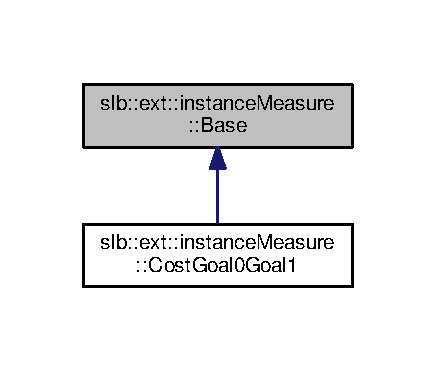
\includegraphics[width=209pt]{structslb_1_1ext_1_1instanceMeasure_1_1Base__inherit__graph}
\end{center}
\end{figure}
\subsubsection*{Public Member Functions}
\begin{DoxyCompactItemize}
\item 
{\footnotesize template$<$class Instance $>$ }\\\hyperlink{structslb_1_1core_1_1sb_1_1MeasureSet}{Measure\+Set} \hyperlink{structslb_1_1ext_1_1instanceMeasure_1_1Base_a254c8bb3b0065ee0bceb4f8b456b7cca}{operator()} (const \hyperlink{structslb_1_1core_1_1sb_1_1Instance}{Instance} \&instance)
\begin{DoxyCompactList}\small\item\em Call operator to compute the measures. \end{DoxyCompactList}\end{DoxyCompactItemize}


\subsubsection{Detailed Description}
One instance measure -- the cost. 

Definition at line 23 of file instance\+\_\+measures.\+h.



\subsubsection{Member Function Documentation}
\index{slb\+::ext\+::instance\+Measure\+::\+Base@{slb\+::ext\+::instance\+Measure\+::\+Base}!operator()@{operator()}}
\index{operator()@{operator()}!slb\+::ext\+::instance\+Measure\+::\+Base@{slb\+::ext\+::instance\+Measure\+::\+Base}}
\paragraph[{\texorpdfstring{operator()(const Instance \&instance)}{operator()(const Instance &instance)}}]{\setlength{\rightskip}{0pt plus 5cm}template$<$class Instance $>$ {\bf Measure\+Set} slb\+::ext\+::instance\+Measure\+::\+Base\+::operator() (
\begin{DoxyParamCaption}
\item[{const {\bf Instance} \&}]{instance}
\end{DoxyParamCaption}
)\hspace{0.3cm}{\ttfamily [inline]}}\hypertarget{structslb_1_1ext_1_1instanceMeasure_1_1Base_a254c8bb3b0065ee0bceb4f8b456b7cca}{}\label{structslb_1_1ext_1_1instanceMeasure_1_1Base_a254c8bb3b0065ee0bceb4f8b456b7cca}


Call operator to compute the measures. 


\begin{DoxyTemplParams}{Template Parameters}
{\em Instance} & The instance type. \\
\hline
\end{DoxyTemplParams}

\begin{DoxyParams}{Parameters}
{\em instance} & The instance. \\
\hline
\end{DoxyParams}
\begin{DoxyReturn}{Returns}
The measures of {\ttfamily instance}. 
\end{DoxyReturn}


Definition at line 29 of file instance\+\_\+measures.\+h.



The documentation for this struct was generated from the following file\+:\begin{DoxyCompactItemize}
\item 
extensions/instance\+\_\+measures/\hyperlink{instance__measures_8h}{instance\+\_\+measures.\+h}\end{DoxyCompactItemize}

\hypertarget{structslb_1_1core_1_1commandLine_1_1Base}{}\subsection{slb\+:\+:core\+:\+:command\+Line\+:\+:Base Struct Reference}
\label{structslb_1_1core_1_1commandLine_1_1Base}\index{slb\+::core\+::command\+Line\+::\+Base@{slb\+::core\+::command\+Line\+::\+Base}}


Holds the command line object. This is needed to initialize the command line object before it is passed to the additions.  




{\ttfamily \#include $<$command\+\_\+line.\+h$>$}



Inheritance diagram for slb\+:\+:core\+:\+:command\+Line\+:\+:Base\+:\nopagebreak
\begin{figure}[H]
\begin{center}
\leavevmode
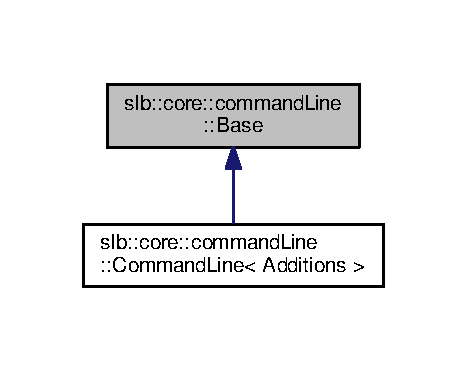
\includegraphics[width=224pt]{structslb_1_1core_1_1commandLine_1_1Base__inherit__graph}
\end{center}
\end{figure}
\subsubsection*{Protected Attributes}
\begin{DoxyCompactItemize}
\item 
T\+C\+L\+A\+P\+::\+Cmd\+Line \hyperlink{structslb_1_1core_1_1commandLine_1_1Base_ac678e3e41ffdfa18846c9fee1c69fdfc}{cmd\+\_\+}\hypertarget{structslb_1_1core_1_1commandLine_1_1Base_ac678e3e41ffdfa18846c9fee1c69fdfc}{}\label{structslb_1_1core_1_1commandLine_1_1Base_ac678e3e41ffdfa18846c9fee1c69fdfc}

\begin{DoxyCompactList}\small\item\em The underlying T\+C\+L\+AP object. \end{DoxyCompactList}\end{DoxyCompactItemize}


\subsubsection{Detailed Description}
Holds the command line object. This is needed to initialize the command line object before it is passed to the additions. 

Definition at line 34 of file command\+\_\+line.\+h.



The documentation for this struct was generated from the following file\+:\begin{DoxyCompactItemize}
\item 
core/\hyperlink{command__line_8h}{command\+\_\+line.\+h}\end{DoxyCompactItemize}

\hypertarget{structslb_1_1ext_1_1node_1_1BaseT}{}\subsection{slb\+:\+:ext\+:\+:node\+:\+:BaseT$<$ State $>$ Struct Template Reference}
\label{structslb_1_1ext_1_1node_1_1BaseT}\index{slb\+::ext\+::node\+::\+Base\+T$<$ State $>$@{slb\+::ext\+::node\+::\+Base\+T$<$ State $>$}}


Regular node storing {\ttfamily g} and {\ttfamily f}.  




{\ttfamily \#include $<$node\+\_\+kinds.\+h$>$}



Inheritance diagram for slb\+:\+:ext\+:\+:node\+:\+:BaseT$<$ State $>$\+:\nopagebreak
\begin{figure}[H]
\begin{center}
\leavevmode
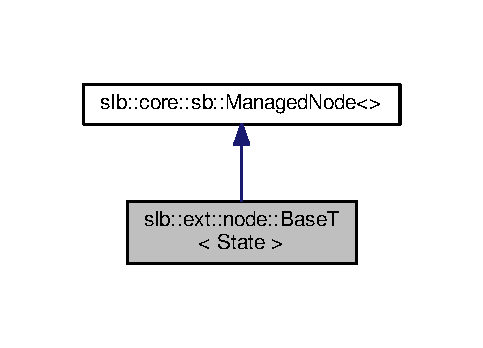
\includegraphics[width=232pt]{structslb_1_1ext_1_1node_1_1BaseT__inherit__graph}
\end{center}
\end{figure}


Collaboration diagram for slb\+:\+:ext\+:\+:node\+:\+:BaseT$<$ State $>$\+:\nopagebreak
\begin{figure}[H]
\begin{center}
\leavevmode
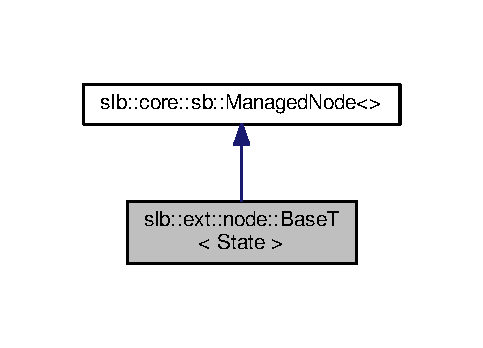
\includegraphics[width=232pt]{structslb_1_1ext_1_1node_1_1BaseT__coll__graph}
\end{center}
\end{figure}
\subsubsection*{Public Types}
\begin{DoxyCompactItemize}
\item 
using \hyperlink{structslb_1_1ext_1_1node_1_1BaseT_a25e9417da3d5610b8d379927697ed848}{Cost\+Type} = typename State\+::\+Cost\+Type\hypertarget{structslb_1_1ext_1_1node_1_1BaseT_a25e9417da3d5610b8d379927697ed848}{}\label{structslb_1_1ext_1_1node_1_1BaseT_a25e9417da3d5610b8d379927697ed848}

\begin{DoxyCompactList}\small\item\em The type representing the cost of actions in the domain. \end{DoxyCompactList}\end{DoxyCompactItemize}
\subsubsection*{Public Member Functions}
\begin{DoxyCompactItemize}
\item 
\hyperlink{structslb_1_1ext_1_1node_1_1BaseT_ada1f4e02d2850b60142fe1ea350b449f}{BaseT} ()\hypertarget{structslb_1_1ext_1_1node_1_1BaseT_ada1f4e02d2850b60142fe1ea350b449f}{}\label{structslb_1_1ext_1_1node_1_1BaseT_ada1f4e02d2850b60142fe1ea350b449f}

\begin{DoxyCompactList}\small\item\em The default constructor. Initializes the node data with zeros. \end{DoxyCompactList}\item 
\hyperlink{structslb_1_1ext_1_1node_1_1BaseT_ab29d45f068f928c9d7faca908e610801}{R\+E\+F\+L\+E\+C\+T\+A\+B\+LE} ((\hyperlink{structslb_1_1ext_1_1node_1_1BaseT_a25e9417da3d5610b8d379927697ed848}{Cost\+Type}) g,(\hyperlink{structslb_1_1ext_1_1node_1_1BaseT_a25e9417da3d5610b8d379927697ed848}{Cost\+Type}) f) \hyperlink{structslb_1_1ext_1_1node_1_1BaseT_a25e9417da3d5610b8d379927697ed848}{Cost\+Type} h() const 
\begin{DoxyCompactList}\small\item\em Returns the heuristic value. \end{DoxyCompactList}\item 
void \hyperlink{structslb_1_1ext_1_1node_1_1BaseT_aa4a669774984fc1f36e459469910c356}{updateG} (\hyperlink{structslb_1_1ext_1_1node_1_1BaseT_a25e9417da3d5610b8d379927697ed848}{Cost\+Type} newG)
\begin{DoxyCompactList}\small\item\em Updates g-\/value of the node. \end{DoxyCompactList}\item 
void \hyperlink{structslb_1_1ext_1_1node_1_1BaseT_ad08ea419ac90831947e8eecf70045dc6}{updateH} (\hyperlink{structslb_1_1ext_1_1node_1_1BaseT_a25e9417da3d5610b8d379927697ed848}{Cost\+Type} newH)
\begin{DoxyCompactList}\small\item\em Updates h-\/value of the node. \end{DoxyCompactList}\item 
void \hyperlink{structslb_1_1ext_1_1node_1_1BaseT_ab2113028f54e4267fa9a613354f3b843}{set} (\hyperlink{structslb_1_1ext_1_1node_1_1BaseT_a25e9417da3d5610b8d379927697ed848}{Cost\+Type} g, \hyperlink{structslb_1_1ext_1_1node_1_1BaseT_a25e9417da3d5610b8d379927697ed848}{Cost\+Type} h, int)
\begin{DoxyCompactList}\small\item\em Sets g and f of the node. \end{DoxyCompactList}\end{DoxyCompactItemize}


\subsubsection{Detailed Description}
\subsubsection*{template$<$class State$>$\\*
struct slb\+::ext\+::node\+::\+Base\+T$<$ State $>$}

Regular node storing {\ttfamily g} and {\ttfamily f}. 


\begin{DoxyTemplParams}{Template Parameters}
{\em State\+\_\+} & The state type, represents the domain. \\
\hline
\end{DoxyTemplParams}


Definition at line 16 of file node\+\_\+kinds.\+h.



\subsubsection{Member Function Documentation}
\index{slb\+::ext\+::node\+::\+BaseT@{slb\+::ext\+::node\+::\+BaseT}!R\+E\+F\+L\+E\+C\+T\+A\+B\+LE@{R\+E\+F\+L\+E\+C\+T\+A\+B\+LE}}
\index{R\+E\+F\+L\+E\+C\+T\+A\+B\+LE@{R\+E\+F\+L\+E\+C\+T\+A\+B\+LE}!slb\+::ext\+::node\+::\+BaseT@{slb\+::ext\+::node\+::\+BaseT}}
\paragraph[{\texorpdfstring{R\+E\+F\+L\+E\+C\+T\+A\+B\+L\+E((\+Cost\+Type) g,(\+Cost\+Type) f) Cost\+Type h() const }{REFLECTABLE((CostType) g,(CostType) f) CostType h() const }}]{\setlength{\rightskip}{0pt plus 5cm}template$<$class State $>$ {\bf slb\+::ext\+::node\+::\+BaseT}$<$ State $>$\+::R\+E\+F\+L\+E\+C\+T\+A\+B\+LE (
\begin{DoxyParamCaption}
\item[{({\bf Cost\+Type})}]{g, }
\item[{({\bf Cost\+Type})}]{f}
\end{DoxyParamCaption}
) const\hspace{0.3cm}{\ttfamily [inline]}}\hypertarget{structslb_1_1ext_1_1node_1_1BaseT_ab29d45f068f928c9d7faca908e610801}{}\label{structslb_1_1ext_1_1node_1_1BaseT_ab29d45f068f928c9d7faca908e610801}


Returns the heuristic value. 

\begin{DoxyReturn}{Returns}
The heuristic value 
\end{DoxyReturn}


Definition at line 22 of file node\+\_\+kinds.\+h.

\index{slb\+::ext\+::node\+::\+BaseT@{slb\+::ext\+::node\+::\+BaseT}!set@{set}}
\index{set@{set}!slb\+::ext\+::node\+::\+BaseT@{slb\+::ext\+::node\+::\+BaseT}}
\paragraph[{\texorpdfstring{set(\+Cost\+Type g, Cost\+Type h, int)}{set(CostType g, CostType h, int)}}]{\setlength{\rightskip}{0pt plus 5cm}template$<$class State $>$ void {\bf slb\+::ext\+::node\+::\+BaseT}$<$ State $>$\+::set (
\begin{DoxyParamCaption}
\item[{{\bf Cost\+Type}}]{g, }
\item[{{\bf Cost\+Type}}]{h, }
\item[{int}]{}
\end{DoxyParamCaption}
)\hspace{0.3cm}{\ttfamily [inline]}}\hypertarget{structslb_1_1ext_1_1node_1_1BaseT_ab2113028f54e4267fa9a613354f3b843}{}\label{structslb_1_1ext_1_1node_1_1BaseT_ab2113028f54e4267fa9a613354f3b843}


Sets g and f of the node. 


\begin{DoxyTemplParams}{Template Parameters}
{\em Node} & The search node type. \\
\hline
\end{DoxyTemplParams}

\begin{DoxyParams}{Parameters}
{\em g} & The g-\/value. \\
\hline
{\em h} & The h-\/value. \\
\hline
\end{DoxyParams}


Definition at line 48 of file node\+\_\+kinds.\+h.

\index{slb\+::ext\+::node\+::\+BaseT@{slb\+::ext\+::node\+::\+BaseT}!updateG@{updateG}}
\index{updateG@{updateG}!slb\+::ext\+::node\+::\+BaseT@{slb\+::ext\+::node\+::\+BaseT}}
\paragraph[{\texorpdfstring{update\+G(\+Cost\+Type new\+G)}{updateG(CostType newG)}}]{\setlength{\rightskip}{0pt plus 5cm}template$<$class State $>$ void {\bf slb\+::ext\+::node\+::\+BaseT}$<$ State $>$\+::updateG (
\begin{DoxyParamCaption}
\item[{{\bf Cost\+Type}}]{newG}
\end{DoxyParamCaption}
)\hspace{0.3cm}{\ttfamily [inline]}}\hypertarget{structslb_1_1ext_1_1node_1_1BaseT_aa4a669774984fc1f36e459469910c356}{}\label{structslb_1_1ext_1_1node_1_1BaseT_aa4a669774984fc1f36e459469910c356}


Updates g-\/value of the node. 


\begin{DoxyParams}{Parameters}
{\em newG} & The new g-\/value. \\
\hline
\end{DoxyParams}


Definition at line 33 of file node\+\_\+kinds.\+h.

\index{slb\+::ext\+::node\+::\+BaseT@{slb\+::ext\+::node\+::\+BaseT}!updateH@{updateH}}
\index{updateH@{updateH}!slb\+::ext\+::node\+::\+BaseT@{slb\+::ext\+::node\+::\+BaseT}}
\paragraph[{\texorpdfstring{update\+H(\+Cost\+Type new\+H)}{updateH(CostType newH)}}]{\setlength{\rightskip}{0pt plus 5cm}template$<$class State $>$ void {\bf slb\+::ext\+::node\+::\+BaseT}$<$ State $>$\+::updateH (
\begin{DoxyParamCaption}
\item[{{\bf Cost\+Type}}]{newH}
\end{DoxyParamCaption}
)\hspace{0.3cm}{\ttfamily [inline]}}\hypertarget{structslb_1_1ext_1_1node_1_1BaseT_ad08ea419ac90831947e8eecf70045dc6}{}\label{structslb_1_1ext_1_1node_1_1BaseT_ad08ea419ac90831947e8eecf70045dc6}


Updates h-\/value of the node. 


\begin{DoxyParams}{Parameters}
{\em newH} & The new h-\/value. \\
\hline
\end{DoxyParams}


Definition at line 40 of file node\+\_\+kinds.\+h.



The documentation for this struct was generated from the following file\+:\begin{DoxyCompactItemize}
\item 
extensions/nodes/\hyperlink{node__kinds_8h}{node\+\_\+kinds.\+h}\end{DoxyCompactItemize}

\hypertarget{structslb_1_1ext_1_1algorithm_1_1BaseTraits}{}\subsection{slb\+:\+:ext\+:\+:algorithm\+:\+:Base\+Traits$<$ A\+L\+G\+\_\+\+T\+P\+A\+R\+A\+MS $>$ Struct Template Reference}
\label{structslb_1_1ext_1_1algorithm_1_1BaseTraits}\index{slb\+::ext\+::algorithm\+::\+Base\+Traits$<$ A\+L\+G\+\_\+\+T\+P\+A\+R\+A\+M\+S $>$@{slb\+::ext\+::algorithm\+::\+Base\+Traits$<$ A\+L\+G\+\_\+\+T\+P\+A\+R\+A\+M\+S $>$}}


Traits shared by all algorithms.  




{\ttfamily \#include $<$algorithm.\+h$>$}

\subsubsection*{Public Types}
\begin{DoxyCompactItemize}
\item 
using \hyperlink{structslb_1_1ext_1_1algorithm_1_1BaseTraits_a4413b287fe7e24a87b1b6bc1bbf5c381}{Node} = Node\+\_\+\hypertarget{structslb_1_1ext_1_1algorithm_1_1BaseTraits_a4413b287fe7e24a87b1b6bc1bbf5c381}{}\label{structslb_1_1ext_1_1algorithm_1_1BaseTraits_a4413b287fe7e24a87b1b6bc1bbf5c381}

\begin{DoxyCompactList}\small\item\em The search node type. \end{DoxyCompactList}\item 
using \hyperlink{structslb_1_1ext_1_1algorithm_1_1BaseTraits_aae4df3d5b38adfe46ebaf725cdaa8399}{Node\+Data} = typename Node\+::\+Node\+Data\hypertarget{structslb_1_1ext_1_1algorithm_1_1BaseTraits_aae4df3d5b38adfe46ebaf725cdaa8399}{}\label{structslb_1_1ext_1_1algorithm_1_1BaseTraits_aae4df3d5b38adfe46ebaf725cdaa8399}

\begin{DoxyCompactList}\small\item\em The type of data stored with a search node. \end{DoxyCompactList}\item 
using \hyperlink{structslb_1_1ext_1_1algorithm_1_1BaseTraits_acde714a3e4695d137190ac4fc7e600c1}{Cost\+Type} = typename Node\+::\+Cost\+Type\hypertarget{structslb_1_1ext_1_1algorithm_1_1BaseTraits_acde714a3e4695d137190ac4fc7e600c1}{}\label{structslb_1_1ext_1_1algorithm_1_1BaseTraits_acde714a3e4695d137190ac4fc7e600c1}

\begin{DoxyCompactList}\small\item\em Type for action cost in the search domain. \end{DoxyCompactList}\item 
using \hyperlink{structslb_1_1ext_1_1algorithm_1_1BaseTraits_ab054296973909aa6bfbe407943f58938}{Return\+Type} = double\hypertarget{structslb_1_1ext_1_1algorithm_1_1BaseTraits_ab054296973909aa6bfbe407943f58938}{}\label{structslb_1_1ext_1_1algorithm_1_1BaseTraits_ab054296973909aa6bfbe407943f58938}

\begin{DoxyCompactList}\small\item\em Type for the return value of the algorithm. Not the same as Cost\+Type due to possible average among several goals. \end{DoxyCompactList}\item 
using \hyperlink{structslb_1_1ext_1_1algorithm_1_1BaseTraits_ab835ffb47510407b9ee0c84e1c4f92a9}{Node\+Unique\+Ptr} = typename Node\+::\+Node\+Unique\+Ptr\hypertarget{structslb_1_1ext_1_1algorithm_1_1BaseTraits_ab835ffb47510407b9ee0c84e1c4f92a9}{}\label{structslb_1_1ext_1_1algorithm_1_1BaseTraits_ab835ffb47510407b9ee0c84e1c4f92a9}

\begin{DoxyCompactList}\small\item\em Unique pointer to search node. \end{DoxyCompactList}\item 
using \hyperlink{structslb_1_1ext_1_1algorithm_1_1BaseTraits_a83eb602d114a921553e8af5db8686ff0}{State} = typename Node\+::\+State\hypertarget{structslb_1_1ext_1_1algorithm_1_1BaseTraits_a83eb602d114a921553e8af5db8686ff0}{}\label{structslb_1_1ext_1_1algorithm_1_1BaseTraits_a83eb602d114a921553e8af5db8686ff0}

\begin{DoxyCompactList}\small\item\em The state type, represents the domain. \end{DoxyCompactList}\item 
using \hyperlink{structslb_1_1ext_1_1algorithm_1_1BaseTraits_a07651b3090a6858cb8bc67afce49c396}{My\+Instance} = \hyperlink{structslb_1_1core_1_1sb_1_1Instance}{Instance}$<$ \hyperlink{structslb_1_1ext_1_1algorithm_1_1BaseTraits_a83eb602d114a921553e8af5db8686ff0}{State} $>$\hypertarget{structslb_1_1ext_1_1algorithm_1_1BaseTraits_a07651b3090a6858cb8bc67afce49c396}{}\label{structslb_1_1ext_1_1algorithm_1_1BaseTraits_a07651b3090a6858cb8bc67afce49c396}

\begin{DoxyCompactList}\small\item\em The problem instance type. \end{DoxyCompactList}\item 
using \hyperlink{structslb_1_1ext_1_1algorithm_1_1BaseTraits_af1ee6f3b936602b3d81b4258c43206bd}{My\+Algorithm\+Log} = typename std\+::conditional$<$ log\+Flag\+\_\+, Algorithm\+Log$<$ \hyperlink{structslb_1_1ext_1_1algorithm_1_1BaseTraits_a4413b287fe7e24a87b1b6bc1bbf5c381}{Node} $>$, \hyperlink{structslb_1_1Nothing}{Nothing} $>$\+::type\hypertarget{structslb_1_1ext_1_1algorithm_1_1BaseTraits_af1ee6f3b936602b3d81b4258c43206bd}{}\label{structslb_1_1ext_1_1algorithm_1_1BaseTraits_af1ee6f3b936602b3d81b4258c43206bd}

\begin{DoxyCompactList}\small\item\em The type for the log of events generated by the algorithm. \end{DoxyCompactList}\end{DoxyCompactItemize}


\subsubsection{Detailed Description}
\subsubsection*{template$<$A\+L\+G\+\_\+\+T\+P\+A\+R\+A\+MS$>$\\*
struct slb\+::ext\+::algorithm\+::\+Base\+Traits$<$ A\+L\+G\+\_\+\+T\+P\+A\+R\+A\+M\+S $>$}

Traits shared by all algorithms. 

Definition at line 68 of file algorithm.\+h.



The documentation for this struct was generated from the following file\+:\begin{DoxyCompactItemize}
\item 
extensions/algorithms/\hyperlink{algorithm_8h}{algorithm.\+h}\end{DoxyCompactItemize}

\hypertarget{structslb_1_1core_1_1util_1_1BasicInformedIterator}{}\subsection{slb\+:\+:core\+:\+:util\+:\+:Basic\+Informed\+Iterator$<$ Container, Base $>$ Struct Template Reference}
\label{structslb_1_1core_1_1util_1_1BasicInformedIterator}\index{slb\+::core\+::util\+::\+Basic\+Informed\+Iterator$<$ Container, Base $>$@{slb\+::core\+::util\+::\+Basic\+Informed\+Iterator$<$ Container, Base $>$}}


Adapter for iterator that knows whether it is at the end.  




{\ttfamily \#include $<$container.\+h$>$}



Inheritance diagram for slb\+:\+:core\+:\+:util\+:\+:Basic\+Informed\+Iterator$<$ Container, Base $>$\+:\nopagebreak
\begin{figure}[H]
\begin{center}
\leavevmode
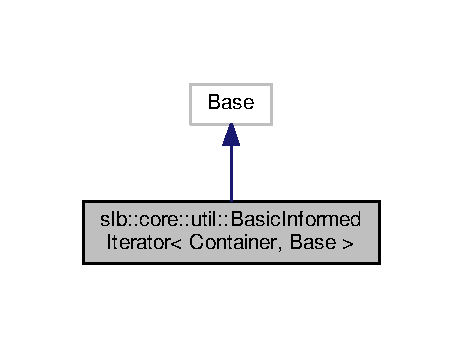
\includegraphics[width=222pt]{structslb_1_1core_1_1util_1_1BasicInformedIterator__inherit__graph}
\end{center}
\end{figure}


Collaboration diagram for slb\+:\+:core\+:\+:util\+:\+:Basic\+Informed\+Iterator$<$ Container, Base $>$\+:\nopagebreak
\begin{figure}[H]
\begin{center}
\leavevmode
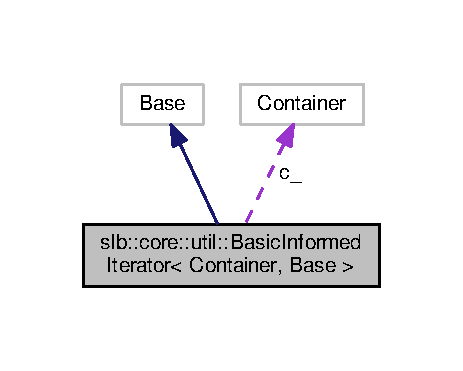
\includegraphics[width=222pt]{structslb_1_1core_1_1util_1_1BasicInformedIterator__coll__graph}
\end{center}
\end{figure}
\subsubsection*{Public Member Functions}
\begin{DoxyCompactItemize}
\item 
\hyperlink{structslb_1_1core_1_1util_1_1BasicInformedIterator_a5df42d0174c2107d33c2c797b6510cd9}{Basic\+Informed\+Iterator} (Container \&c)
\begin{DoxyCompactList}\small\item\em Constructor. \end{DoxyCompactList}\item 
\hyperlink{structslb_1_1core_1_1util_1_1BasicInformedIterator_a1703216a7bd1c0d0a0dd02ed5a946ad9}{Basic\+Informed\+Iterator} (Container \&c, Base b)
\begin{DoxyCompactList}\small\item\em Constructor based on the given base iterator. \end{DoxyCompactList}\item 
\hyperlink{structslb_1_1core_1_1util_1_1BasicInformedIterator_ad87320b140e204fb3a1878ec244fbab2}{Basic\+Informed\+Iterator} (const \hyperlink{structslb_1_1core_1_1util_1_1BasicInformedIterator}{Basic\+Informed\+Iterator} \&b)
\begin{DoxyCompactList}\small\item\em Copy constructor. \end{DoxyCompactList}\item 
bool \hyperlink{structslb_1_1core_1_1util_1_1BasicInformedIterator_ac9c0870a0d2ecea6c987c0c461afb15d}{is\+Begin} () const 
\begin{DoxyCompactList}\small\item\em Checks whether the iterator is at the beginning of the container. \end{DoxyCompactList}\item 
bool \hyperlink{structslb_1_1core_1_1util_1_1BasicInformedIterator_a4a41e1c9f51ce3d202a0c010cefe5984}{is\+End} () const 
\begin{DoxyCompactList}\small\item\em Checks whether the iterator is at the end of the container. \end{DoxyCompactList}\item 
Container \& \hyperlink{structslb_1_1core_1_1util_1_1BasicInformedIterator_a110589c99038df127259fb2e17cb2ba3}{container} () const 
\begin{DoxyCompactList}\small\item\em Returns reference to the underlying container. \end{DoxyCompactList}\item 
\hyperlink{structslb_1_1core_1_1util_1_1BasicInformedIterator}{Basic\+Informed\+Iterator} \& \hyperlink{structslb_1_1core_1_1util_1_1BasicInformedIterator_a9f6c85b4389b4e023fb68c3817a22c4d}{operator=} (const \hyperlink{structslb_1_1core_1_1util_1_1BasicInformedIterator}{Basic\+Informed\+Iterator} \&rhs)
\begin{DoxyCompactList}\small\item\em The assignment operator. \end{DoxyCompactList}\item 
int \hyperlink{structslb_1_1core_1_1util_1_1BasicInformedIterator_a50d044b0f6b994f5bdd0e6fed3660f6e}{index} () const 
\begin{DoxyCompactList}\small\item\em Computes the index corresponding to the iterator. \end{DoxyCompactList}\end{DoxyCompactItemize}
\subsubsection*{Private Attributes}
\begin{DoxyCompactItemize}
\item 
Container \& \hyperlink{structslb_1_1core_1_1util_1_1BasicInformedIterator_a917c20e6bce46eb0666bd58c5371af53}{c\+\_\+}\hypertarget{structslb_1_1core_1_1util_1_1BasicInformedIterator_a917c20e6bce46eb0666bd58c5371af53}{}\label{structslb_1_1core_1_1util_1_1BasicInformedIterator_a917c20e6bce46eb0666bd58c5371af53}

\begin{DoxyCompactList}\small\item\em The underlying container. \end{DoxyCompactList}\end{DoxyCompactItemize}


\subsubsection{Detailed Description}
\subsubsection*{template$<$class Container, class Base$>$\\*
struct slb\+::core\+::util\+::\+Basic\+Informed\+Iterator$<$ Container, Base $>$}

Adapter for iterator that knows whether it is at the end. 


\begin{DoxyTemplParams}{Template Parameters}
{\em Container} & The underlying container type. \\
\hline
{\em Base} & The base iterator, can be Constainer\+::iterator or Container\+::const\+\_\+iterator. \\
\hline
\end{DoxyTemplParams}


Definition at line 109 of file container.\+h.



\subsubsection{Constructor \& Destructor Documentation}
\index{slb\+::core\+::util\+::\+Basic\+Informed\+Iterator@{slb\+::core\+::util\+::\+Basic\+Informed\+Iterator}!Basic\+Informed\+Iterator@{Basic\+Informed\+Iterator}}
\index{Basic\+Informed\+Iterator@{Basic\+Informed\+Iterator}!slb\+::core\+::util\+::\+Basic\+Informed\+Iterator@{slb\+::core\+::util\+::\+Basic\+Informed\+Iterator}}
\paragraph[{\texorpdfstring{Basic\+Informed\+Iterator(\+Container \&c)}{BasicInformedIterator(Container &c)}}]{\setlength{\rightskip}{0pt plus 5cm}template$<$class Container, class Base$>$ {\bf slb\+::core\+::util\+::\+Basic\+Informed\+Iterator}$<$ Container, Base $>$\+::{\bf Basic\+Informed\+Iterator} (
\begin{DoxyParamCaption}
\item[{Container \&}]{c}
\end{DoxyParamCaption}
)\hspace{0.3cm}{\ttfamily [inline]}}\hypertarget{structslb_1_1core_1_1util_1_1BasicInformedIterator_a5df42d0174c2107d33c2c797b6510cd9}{}\label{structslb_1_1core_1_1util_1_1BasicInformedIterator_a5df42d0174c2107d33c2c797b6510cd9}


Constructor. 


\begin{DoxyParams}{Parameters}
{\em c} & Reference to the container. \\
\hline
\end{DoxyParams}


Definition at line 112 of file container.\+h.

\index{slb\+::core\+::util\+::\+Basic\+Informed\+Iterator@{slb\+::core\+::util\+::\+Basic\+Informed\+Iterator}!Basic\+Informed\+Iterator@{Basic\+Informed\+Iterator}}
\index{Basic\+Informed\+Iterator@{Basic\+Informed\+Iterator}!slb\+::core\+::util\+::\+Basic\+Informed\+Iterator@{slb\+::core\+::util\+::\+Basic\+Informed\+Iterator}}
\paragraph[{\texorpdfstring{Basic\+Informed\+Iterator(\+Container \&c, Base b)}{BasicInformedIterator(Container &c, Base b)}}]{\setlength{\rightskip}{0pt plus 5cm}template$<$class Container, class Base$>$ {\bf slb\+::core\+::util\+::\+Basic\+Informed\+Iterator}$<$ Container, Base $>$\+::{\bf Basic\+Informed\+Iterator} (
\begin{DoxyParamCaption}
\item[{Container \&}]{c, }
\item[{Base}]{b}
\end{DoxyParamCaption}
)\hspace{0.3cm}{\ttfamily [inline]}}\hypertarget{structslb_1_1core_1_1util_1_1BasicInformedIterator_a1703216a7bd1c0d0a0dd02ed5a946ad9}{}\label{structslb_1_1core_1_1util_1_1BasicInformedIterator_a1703216a7bd1c0d0a0dd02ed5a946ad9}


Constructor based on the given base iterator. 


\begin{DoxyParams}{Parameters}
{\em c} & Reference to the container. \\
\hline
{\em b} & Base iterator. \\
\hline
\end{DoxyParams}


Definition at line 117 of file container.\+h.

\index{slb\+::core\+::util\+::\+Basic\+Informed\+Iterator@{slb\+::core\+::util\+::\+Basic\+Informed\+Iterator}!Basic\+Informed\+Iterator@{Basic\+Informed\+Iterator}}
\index{Basic\+Informed\+Iterator@{Basic\+Informed\+Iterator}!slb\+::core\+::util\+::\+Basic\+Informed\+Iterator@{slb\+::core\+::util\+::\+Basic\+Informed\+Iterator}}
\paragraph[{\texorpdfstring{Basic\+Informed\+Iterator(const Basic\+Informed\+Iterator \&b)}{BasicInformedIterator(const BasicInformedIterator &b)}}]{\setlength{\rightskip}{0pt plus 5cm}template$<$class Container, class Base$>$ {\bf slb\+::core\+::util\+::\+Basic\+Informed\+Iterator}$<$ Container, Base $>$\+::{\bf Basic\+Informed\+Iterator} (
\begin{DoxyParamCaption}
\item[{const {\bf Basic\+Informed\+Iterator}$<$ Container, Base $>$ \&}]{b}
\end{DoxyParamCaption}
)\hspace{0.3cm}{\ttfamily [inline]}}\hypertarget{structslb_1_1core_1_1util_1_1BasicInformedIterator_ad87320b140e204fb3a1878ec244fbab2}{}\label{structslb_1_1core_1_1util_1_1BasicInformedIterator_ad87320b140e204fb3a1878ec244fbab2}


Copy constructor. 


\begin{DoxyParams}{Parameters}
{\em b} & The given iterator. \\
\hline
\end{DoxyParams}


Definition at line 121 of file container.\+h.



\subsubsection{Member Function Documentation}
\index{slb\+::core\+::util\+::\+Basic\+Informed\+Iterator@{slb\+::core\+::util\+::\+Basic\+Informed\+Iterator}!container@{container}}
\index{container@{container}!slb\+::core\+::util\+::\+Basic\+Informed\+Iterator@{slb\+::core\+::util\+::\+Basic\+Informed\+Iterator}}
\paragraph[{\texorpdfstring{container() const }{container() const }}]{\setlength{\rightskip}{0pt plus 5cm}template$<$class Container, class Base$>$ Container\& {\bf slb\+::core\+::util\+::\+Basic\+Informed\+Iterator}$<$ Container, Base $>$\+::container (
\begin{DoxyParamCaption}
{}
\end{DoxyParamCaption}
) const\hspace{0.3cm}{\ttfamily [inline]}}\hypertarget{structslb_1_1core_1_1util_1_1BasicInformedIterator_a110589c99038df127259fb2e17cb2ba3}{}\label{structslb_1_1core_1_1util_1_1BasicInformedIterator_a110589c99038df127259fb2e17cb2ba3}


Returns reference to the underlying container. 

\begin{DoxyReturn}{Returns}
Reference to the underlying container. 
\end{DoxyReturn}


Definition at line 135 of file container.\+h.

\index{slb\+::core\+::util\+::\+Basic\+Informed\+Iterator@{slb\+::core\+::util\+::\+Basic\+Informed\+Iterator}!index@{index}}
\index{index@{index}!slb\+::core\+::util\+::\+Basic\+Informed\+Iterator@{slb\+::core\+::util\+::\+Basic\+Informed\+Iterator}}
\paragraph[{\texorpdfstring{index() const }{index() const }}]{\setlength{\rightskip}{0pt plus 5cm}template$<$class Container, class Base$>$ int {\bf slb\+::core\+::util\+::\+Basic\+Informed\+Iterator}$<$ Container, Base $>$\+::index (
\begin{DoxyParamCaption}
{}
\end{DoxyParamCaption}
) const\hspace{0.3cm}{\ttfamily [inline]}}\hypertarget{structslb_1_1core_1_1util_1_1BasicInformedIterator_a50d044b0f6b994f5bdd0e6fed3660f6e}{}\label{structslb_1_1core_1_1util_1_1BasicInformedIterator_a50d044b0f6b994f5bdd0e6fed3660f6e}


Computes the index corresponding to the iterator. 

\begin{DoxyReturn}{Returns}
The index corresponding to the iterator. 
\end{DoxyReturn}


Definition at line 148 of file container.\+h.

\index{slb\+::core\+::util\+::\+Basic\+Informed\+Iterator@{slb\+::core\+::util\+::\+Basic\+Informed\+Iterator}!is\+Begin@{is\+Begin}}
\index{is\+Begin@{is\+Begin}!slb\+::core\+::util\+::\+Basic\+Informed\+Iterator@{slb\+::core\+::util\+::\+Basic\+Informed\+Iterator}}
\paragraph[{\texorpdfstring{is\+Begin() const }{isBegin() const }}]{\setlength{\rightskip}{0pt plus 5cm}template$<$class Container, class Base$>$ bool {\bf slb\+::core\+::util\+::\+Basic\+Informed\+Iterator}$<$ Container, Base $>$\+::is\+Begin (
\begin{DoxyParamCaption}
{}
\end{DoxyParamCaption}
) const\hspace{0.3cm}{\ttfamily [inline]}}\hypertarget{structslb_1_1core_1_1util_1_1BasicInformedIterator_ac9c0870a0d2ecea6c987c0c461afb15d}{}\label{structslb_1_1core_1_1util_1_1BasicInformedIterator_ac9c0870a0d2ecea6c987c0c461afb15d}


Checks whether the iterator is at the beginning of the container. 

\begin{DoxyReturn}{Returns}
{\ttfamily true} if the iterator is at the beginning of the container and {\ttfamily false} otherwise. 
\end{DoxyReturn}


Definition at line 126 of file container.\+h.

\index{slb\+::core\+::util\+::\+Basic\+Informed\+Iterator@{slb\+::core\+::util\+::\+Basic\+Informed\+Iterator}!is\+End@{is\+End}}
\index{is\+End@{is\+End}!slb\+::core\+::util\+::\+Basic\+Informed\+Iterator@{slb\+::core\+::util\+::\+Basic\+Informed\+Iterator}}
\paragraph[{\texorpdfstring{is\+End() const }{isEnd() const }}]{\setlength{\rightskip}{0pt plus 5cm}template$<$class Container, class Base$>$ bool {\bf slb\+::core\+::util\+::\+Basic\+Informed\+Iterator}$<$ Container, Base $>$\+::is\+End (
\begin{DoxyParamCaption}
{}
\end{DoxyParamCaption}
) const\hspace{0.3cm}{\ttfamily [inline]}}\hypertarget{structslb_1_1core_1_1util_1_1BasicInformedIterator_a4a41e1c9f51ce3d202a0c010cefe5984}{}\label{structslb_1_1core_1_1util_1_1BasicInformedIterator_a4a41e1c9f51ce3d202a0c010cefe5984}


Checks whether the iterator is at the end of the container. 

\begin{DoxyReturn}{Returns}
{\ttfamily true} if the iterator is at the end of the container and {\ttfamily false} otherwise. 
\end{DoxyReturn}


Definition at line 131 of file container.\+h.

\index{slb\+::core\+::util\+::\+Basic\+Informed\+Iterator@{slb\+::core\+::util\+::\+Basic\+Informed\+Iterator}!operator=@{operator=}}
\index{operator=@{operator=}!slb\+::core\+::util\+::\+Basic\+Informed\+Iterator@{slb\+::core\+::util\+::\+Basic\+Informed\+Iterator}}
\paragraph[{\texorpdfstring{operator=(const Basic\+Informed\+Iterator \&rhs)}{operator=(const BasicInformedIterator &rhs)}}]{\setlength{\rightskip}{0pt plus 5cm}template$<$class Container, class Base$>$ {\bf Basic\+Informed\+Iterator}\& {\bf slb\+::core\+::util\+::\+Basic\+Informed\+Iterator}$<$ Container, Base $>$\+::operator= (
\begin{DoxyParamCaption}
\item[{const {\bf Basic\+Informed\+Iterator}$<$ Container, Base $>$ \&}]{rhs}
\end{DoxyParamCaption}
)\hspace{0.3cm}{\ttfamily [inline]}}\hypertarget{structslb_1_1core_1_1util_1_1BasicInformedIterator_a9f6c85b4389b4e023fb68c3817a22c4d}{}\label{structslb_1_1core_1_1util_1_1BasicInformedIterator_a9f6c85b4389b4e023fb68c3817a22c4d}


The assignment operator. 


\begin{DoxyParams}{Parameters}
{\em rhs} & The right-\/hand side iterator. \\
\hline
\end{DoxyParams}
\begin{DoxyReturn}{Returns}
Reference to the resulting iterator. 
\end{DoxyReturn}


Definition at line 140 of file container.\+h.



The documentation for this struct was generated from the following file\+:\begin{DoxyCompactItemize}
\item 
core/util/\hyperlink{container_8h}{container.\+h}\end{DoxyCompactItemize}

\hypertarget{structslb_1_1core_1_1util_1_1BasicVectorSkipIterator}{}\subsection{slb\+:\+:core\+:\+:util\+:\+:Basic\+Vector\+Skip\+Iterator$<$ My\+Vector, Base\+Iterator $>$ Struct Template Reference}
\label{structslb_1_1core_1_1util_1_1BasicVectorSkipIterator}\index{slb\+::core\+::util\+::\+Basic\+Vector\+Skip\+Iterator$<$ My\+Vector, Base\+Iterator $>$@{slb\+::core\+::util\+::\+Basic\+Vector\+Skip\+Iterator$<$ My\+Vector, Base\+Iterator $>$}}


Iterator for a vector that skips a certain value.  




{\ttfamily \#include $<$container.\+h$>$}



Inheritance diagram for slb\+:\+:core\+:\+:util\+:\+:Basic\+Vector\+Skip\+Iterator$<$ My\+Vector, Base\+Iterator $>$\+:\nopagebreak
\begin{figure}[H]
\begin{center}
\leavevmode
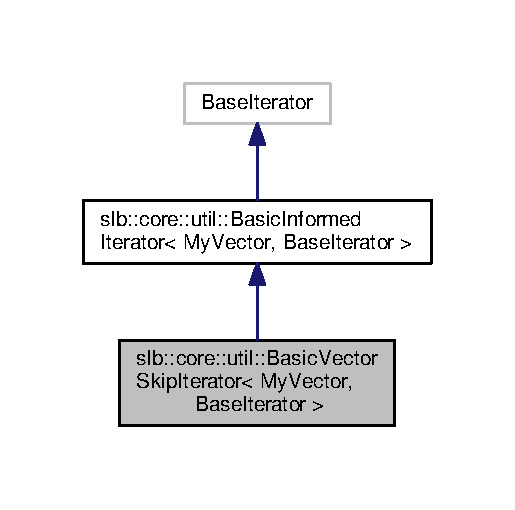
\includegraphics[width=247pt]{structslb_1_1core_1_1util_1_1BasicVectorSkipIterator__inherit__graph}
\end{center}
\end{figure}


Collaboration diagram for slb\+:\+:core\+:\+:util\+:\+:Basic\+Vector\+Skip\+Iterator$<$ My\+Vector, Base\+Iterator $>$\+:\nopagebreak
\begin{figure}[H]
\begin{center}
\leavevmode
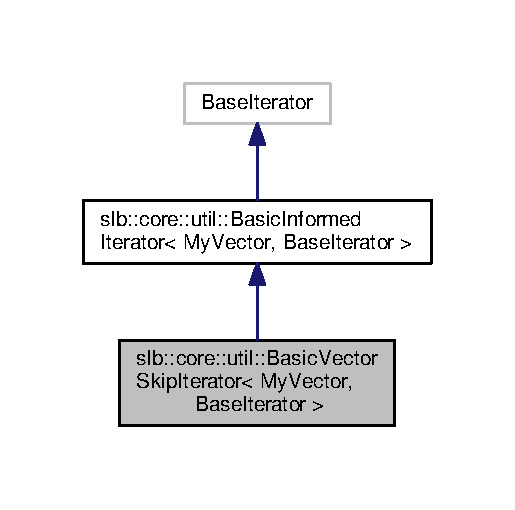
\includegraphics[width=247pt]{structslb_1_1core_1_1util_1_1BasicVectorSkipIterator__coll__graph}
\end{center}
\end{figure}
\subsubsection*{Public Types}
\begin{DoxyCompactItemize}
\item 
using \hyperlink{structslb_1_1core_1_1util_1_1BasicVectorSkipIterator_a1f81c5bdd82df852058bc0396ac54514}{Base} = \hyperlink{structslb_1_1core_1_1util_1_1BasicInformedIterator}{Basic\+Informed\+Iterator}$<$ My\+Vector, Base\+Iterator $>$\hypertarget{structslb_1_1core_1_1util_1_1BasicVectorSkipIterator_a1f81c5bdd82df852058bc0396ac54514}{}\label{structslb_1_1core_1_1util_1_1BasicVectorSkipIterator_a1f81c5bdd82df852058bc0396ac54514}

\begin{DoxyCompactList}\small\item\em The informed iterator, on which this skipping iterator is based. \end{DoxyCompactList}\item 
using \hyperlink{structslb_1_1core_1_1util_1_1BasicVectorSkipIterator_afa39da0ab694b51d0abd089e7612a763}{Value\+Type} = typename My\+Vector\+::value\+\_\+type\hypertarget{structslb_1_1core_1_1util_1_1BasicVectorSkipIterator_afa39da0ab694b51d0abd089e7612a763}{}\label{structslb_1_1core_1_1util_1_1BasicVectorSkipIterator_afa39da0ab694b51d0abd089e7612a763}

\begin{DoxyCompactList}\small\item\em The type of values stored in the vector. \end{DoxyCompactList}\end{DoxyCompactItemize}
\subsubsection*{Public Member Functions}
\begin{DoxyCompactItemize}
\item 
\hyperlink{structslb_1_1core_1_1util_1_1BasicVectorSkipIterator_aa46df09e95807f6b4bc749a84e13e2e5}{Basic\+Vector\+Skip\+Iterator} (My\+Vector \&v, Base\+Iterator it, const \hyperlink{structslb_1_1core_1_1util_1_1BasicVectorSkipIterator_afa39da0ab694b51d0abd089e7612a763}{Value\+Type} \&skip)
\begin{DoxyCompactList}\small\item\em Constructor. \end{DoxyCompactList}\item 
\hyperlink{structslb_1_1core_1_1util_1_1BasicVectorSkipIterator_ac265c697274c7d7791b1a7d8bf9a7370}{Basic\+Vector\+Skip\+Iterator} (const \hyperlink{structslb_1_1core_1_1util_1_1BasicVectorSkipIterator}{Basic\+Vector\+Skip\+Iterator} \&b)
\begin{DoxyCompactList}\small\item\em The copy constructor. \end{DoxyCompactList}\item 
\hyperlink{structslb_1_1core_1_1util_1_1BasicVectorSkipIterator}{Basic\+Vector\+Skip\+Iterator} \& \hyperlink{structslb_1_1core_1_1util_1_1BasicVectorSkipIterator_a3e4ab47663d9a7e1ef957162845e7653}{operator++} ()
\begin{DoxyCompactList}\small\item\em Advance operator. \end{DoxyCompactList}\item 
\hyperlink{structslb_1_1core_1_1util_1_1BasicVectorSkipIterator}{Basic\+Vector\+Skip\+Iterator} \& \hyperlink{structslb_1_1core_1_1util_1_1BasicVectorSkipIterator_a7c20091a03321d6e6b26f8bf16e4a037}{operator=} (const \hyperlink{structslb_1_1core_1_1util_1_1BasicVectorSkipIterator}{Basic\+Vector\+Skip\+Iterator} \&rhs)
\begin{DoxyCompactList}\small\item\em The assignment operator. \end{DoxyCompactList}\end{DoxyCompactItemize}
\subsubsection*{Private Member Functions}
\begin{DoxyCompactItemize}
\item 
void \hyperlink{structslb_1_1core_1_1util_1_1BasicVectorSkipIterator_a62b9c795de2c431982e105887b335f29}{adjust} ()\hypertarget{structslb_1_1core_1_1util_1_1BasicVectorSkipIterator_a62b9c795de2c431982e105887b335f29}{}\label{structslb_1_1core_1_1util_1_1BasicVectorSkipIterator_a62b9c795de2c431982e105887b335f29}

\begin{DoxyCompactList}\small\item\em Adjusts the iterator to point to an element that is not to be skipped or to the end of the container. \end{DoxyCompactList}\end{DoxyCompactItemize}
\subsubsection*{Private Attributes}
\begin{DoxyCompactItemize}
\item 
\hyperlink{structslb_1_1core_1_1util_1_1BasicVectorSkipIterator_afa39da0ab694b51d0abd089e7612a763}{Value\+Type} \hyperlink{structslb_1_1core_1_1util_1_1BasicVectorSkipIterator_ae135631575e5e7b7275e26163f4a55d0}{skip\+\_\+}\hypertarget{structslb_1_1core_1_1util_1_1BasicVectorSkipIterator_ae135631575e5e7b7275e26163f4a55d0}{}\label{structslb_1_1core_1_1util_1_1BasicVectorSkipIterator_ae135631575e5e7b7275e26163f4a55d0}

\begin{DoxyCompactList}\small\item\em The value to be skipped. \end{DoxyCompactList}\end{DoxyCompactItemize}


\subsubsection{Detailed Description}
\subsubsection*{template$<$class My\+Vector, class Base\+Iterator$>$\\*
struct slb\+::core\+::util\+::\+Basic\+Vector\+Skip\+Iterator$<$ My\+Vector, Base\+Iterator $>$}

Iterator for a vector that skips a certain value. 


\begin{DoxyTemplParams}{Template Parameters}
{\em My\+Vector} & The underlying vector type. \\
\hline
{\em Base} & The base iterator, can be My\+Vector\+::iterator or My\+Vector\+::const\+\_\+iterator. \\
\hline
\end{DoxyTemplParams}


Definition at line 159 of file container.\+h.



\subsubsection{Constructor \& Destructor Documentation}
\index{slb\+::core\+::util\+::\+Basic\+Vector\+Skip\+Iterator@{slb\+::core\+::util\+::\+Basic\+Vector\+Skip\+Iterator}!Basic\+Vector\+Skip\+Iterator@{Basic\+Vector\+Skip\+Iterator}}
\index{Basic\+Vector\+Skip\+Iterator@{Basic\+Vector\+Skip\+Iterator}!slb\+::core\+::util\+::\+Basic\+Vector\+Skip\+Iterator@{slb\+::core\+::util\+::\+Basic\+Vector\+Skip\+Iterator}}
\paragraph[{\texorpdfstring{Basic\+Vector\+Skip\+Iterator(\+My\+Vector \&v, Base\+Iterator it, const Value\+Type \&skip)}{BasicVectorSkipIterator(MyVector &v, BaseIterator it, const ValueType &skip)}}]{\setlength{\rightskip}{0pt plus 5cm}template$<$class My\+Vector , class Base\+Iterator $>$ {\bf slb\+::core\+::util\+::\+Basic\+Vector\+Skip\+Iterator}$<$ My\+Vector, Base\+Iterator $>$\+::{\bf Basic\+Vector\+Skip\+Iterator} (
\begin{DoxyParamCaption}
\item[{My\+Vector \&}]{v, }
\item[{Base\+Iterator}]{it, }
\item[{const {\bf Value\+Type} \&}]{skip}
\end{DoxyParamCaption}
)\hspace{0.3cm}{\ttfamily [inline]}}\hypertarget{structslb_1_1core_1_1util_1_1BasicVectorSkipIterator_aa46df09e95807f6b4bc749a84e13e2e5}{}\label{structslb_1_1core_1_1util_1_1BasicVectorSkipIterator_aa46df09e95807f6b4bc749a84e13e2e5}


Constructor. 


\begin{DoxyParams}{Parameters}
{\em v} & The underlying vector. \\
\hline
{\em it} & The initial iteration position, which is adjusted by the constructor to point to an element that is not to be skipped. \\
\hline
{\em skip} & The value to be skipped. \\
\hline
\end{DoxyParams}


Definition at line 171 of file container.\+h.

\index{slb\+::core\+::util\+::\+Basic\+Vector\+Skip\+Iterator@{slb\+::core\+::util\+::\+Basic\+Vector\+Skip\+Iterator}!Basic\+Vector\+Skip\+Iterator@{Basic\+Vector\+Skip\+Iterator}}
\index{Basic\+Vector\+Skip\+Iterator@{Basic\+Vector\+Skip\+Iterator}!slb\+::core\+::util\+::\+Basic\+Vector\+Skip\+Iterator@{slb\+::core\+::util\+::\+Basic\+Vector\+Skip\+Iterator}}
\paragraph[{\texorpdfstring{Basic\+Vector\+Skip\+Iterator(const Basic\+Vector\+Skip\+Iterator \&b)}{BasicVectorSkipIterator(const BasicVectorSkipIterator &b)}}]{\setlength{\rightskip}{0pt plus 5cm}template$<$class My\+Vector , class Base\+Iterator $>$ {\bf slb\+::core\+::util\+::\+Basic\+Vector\+Skip\+Iterator}$<$ My\+Vector, Base\+Iterator $>$\+::{\bf Basic\+Vector\+Skip\+Iterator} (
\begin{DoxyParamCaption}
\item[{const {\bf Basic\+Vector\+Skip\+Iterator}$<$ My\+Vector, Base\+Iterator $>$ \&}]{b}
\end{DoxyParamCaption}
)\hspace{0.3cm}{\ttfamily [inline]}}\hypertarget{structslb_1_1core_1_1util_1_1BasicVectorSkipIterator_ac265c697274c7d7791b1a7d8bf9a7370}{}\label{structslb_1_1core_1_1util_1_1BasicVectorSkipIterator_ac265c697274c7d7791b1a7d8bf9a7370}


The copy constructor. 


\begin{DoxyParams}{Parameters}
{\em b} & The given skipping iterator. \\
\hline
\end{DoxyParams}


Definition at line 178 of file container.\+h.



\subsubsection{Member Function Documentation}
\index{slb\+::core\+::util\+::\+Basic\+Vector\+Skip\+Iterator@{slb\+::core\+::util\+::\+Basic\+Vector\+Skip\+Iterator}!operator++@{operator++}}
\index{operator++@{operator++}!slb\+::core\+::util\+::\+Basic\+Vector\+Skip\+Iterator@{slb\+::core\+::util\+::\+Basic\+Vector\+Skip\+Iterator}}
\paragraph[{\texorpdfstring{operator++()}{operator++()}}]{\setlength{\rightskip}{0pt plus 5cm}template$<$class My\+Vector , class Base\+Iterator $>$ {\bf Basic\+Vector\+Skip\+Iterator}\& {\bf slb\+::core\+::util\+::\+Basic\+Vector\+Skip\+Iterator}$<$ My\+Vector, Base\+Iterator $>$\+::operator++ (
\begin{DoxyParamCaption}
{}
\end{DoxyParamCaption}
)\hspace{0.3cm}{\ttfamily [inline]}}\hypertarget{structslb_1_1core_1_1util_1_1BasicVectorSkipIterator_a3e4ab47663d9a7e1ef957162845e7653}{}\label{structslb_1_1core_1_1util_1_1BasicVectorSkipIterator_a3e4ab47663d9a7e1ef957162845e7653}


Advance operator. 

\begin{DoxyReturn}{Returns}
Reference to the resulting iterator. 
\end{DoxyReturn}


Definition at line 183 of file container.\+h.

\index{slb\+::core\+::util\+::\+Basic\+Vector\+Skip\+Iterator@{slb\+::core\+::util\+::\+Basic\+Vector\+Skip\+Iterator}!operator=@{operator=}}
\index{operator=@{operator=}!slb\+::core\+::util\+::\+Basic\+Vector\+Skip\+Iterator@{slb\+::core\+::util\+::\+Basic\+Vector\+Skip\+Iterator}}
\paragraph[{\texorpdfstring{operator=(const Basic\+Vector\+Skip\+Iterator \&rhs)}{operator=(const BasicVectorSkipIterator &rhs)}}]{\setlength{\rightskip}{0pt plus 5cm}template$<$class My\+Vector , class Base\+Iterator $>$ {\bf Basic\+Vector\+Skip\+Iterator}\& {\bf slb\+::core\+::util\+::\+Basic\+Vector\+Skip\+Iterator}$<$ My\+Vector, Base\+Iterator $>$\+::operator= (
\begin{DoxyParamCaption}
\item[{const {\bf Basic\+Vector\+Skip\+Iterator}$<$ My\+Vector, Base\+Iterator $>$ \&}]{rhs}
\end{DoxyParamCaption}
)\hspace{0.3cm}{\ttfamily [inline]}}\hypertarget{structslb_1_1core_1_1util_1_1BasicVectorSkipIterator_a7c20091a03321d6e6b26f8bf16e4a037}{}\label{structslb_1_1core_1_1util_1_1BasicVectorSkipIterator_a7c20091a03321d6e6b26f8bf16e4a037}


The assignment operator. 


\begin{DoxyParams}{Parameters}
{\em rhs} & The right-\/hand side iterator. \\
\hline
\end{DoxyParams}
\begin{DoxyReturn}{Returns}
Reference to the resulting iterator. 
\end{DoxyReturn}


Definition at line 192 of file container.\+h.



The documentation for this struct was generated from the following file\+:\begin{DoxyCompactItemize}
\item 
core/util/\hyperlink{container_8h}{container.\+h}\end{DoxyCompactItemize}

\hypertarget{structslb_1_1ext_1_1policy_1_1openList_1_1BucketedStdMap__T}{}\subsection{slb\+:\+:ext\+:\+:policy\+:\+:open\+List\+:\+:Bucketed\+Std\+Map\+\_\+T$<$ My\+Algorithm\+\_\+, Node\+\_\+, Key\+Type\+\_\+, Greater\+Priority\+\_\+, Container $>$ Struct Template Reference}
\label{structslb_1_1ext_1_1policy_1_1openList_1_1BucketedStdMap__T}\index{slb\+::ext\+::policy\+::open\+List\+::\+Bucketed\+Std\+Map\+\_\+\+T$<$ My\+Algorithm\+\_\+, Node\+\_\+, Key\+Type\+\_\+, Greater\+Priority\+\_\+, Container $>$@{slb\+::ext\+::policy\+::open\+List\+::\+Bucketed\+Std\+Map\+\_\+\+T$<$ My\+Algorithm\+\_\+, Node\+\_\+, Key\+Type\+\_\+, Greater\+Priority\+\_\+, Container $>$}}


A flexible open list base on {\ttfamily std\+::map} whose values are buckets of nodes with same priority.  




{\ttfamily \#include $<$open\+\_\+list.\+h$>$}

\subsubsection*{Public Types}
\begin{DoxyCompactItemize}
\item 
using \hyperlink{structslb_1_1ext_1_1policy_1_1openList_1_1BucketedStdMap__T_abe8c12b881c4c3440e5b5e3aaa72c061}{My\+Algorithm} = My\+Algorithm\+\_\+\hypertarget{structslb_1_1ext_1_1policy_1_1openList_1_1BucketedStdMap__T_abe8c12b881c4c3440e5b5e3aaa72c061}{}\label{structslb_1_1ext_1_1policy_1_1openList_1_1BucketedStdMap__T_abe8c12b881c4c3440e5b5e3aaa72c061}

\begin{DoxyCompactList}\small\item\em The search algorithm type. \end{DoxyCompactList}\item 
using \hyperlink{structslb_1_1ext_1_1policy_1_1openList_1_1BucketedStdMap__T_aa301ab635e2de1a7c0a67776e4239ec6}{Bucket\+Position} = int\hypertarget{structslb_1_1ext_1_1policy_1_1openList_1_1BucketedStdMap__T_aa301ab635e2de1a7c0a67776e4239ec6}{}\label{structslb_1_1ext_1_1policy_1_1openList_1_1BucketedStdMap__T_aa301ab635e2de1a7c0a67776e4239ec6}

\begin{DoxyCompactList}\small\item\em Type for storing node position in the open list. \end{DoxyCompactList}\item 
using \hyperlink{structslb_1_1ext_1_1policy_1_1openList_1_1BucketedStdMap__T_a20be12bd955d752d2ef9e78f7577c738}{Node} = Node\+\_\+\hypertarget{structslb_1_1ext_1_1policy_1_1openList_1_1BucketedStdMap__T_a20be12bd955d752d2ef9e78f7577c738}{}\label{structslb_1_1ext_1_1policy_1_1openList_1_1BucketedStdMap__T_a20be12bd955d752d2ef9e78f7577c738}

\begin{DoxyCompactList}\small\item\em The node type. \end{DoxyCompactList}\item 
using \hyperlink{structslb_1_1ext_1_1policy_1_1openList_1_1BucketedStdMap__T_a1236fe314465155339798c0f9c4c5ca8}{Key\+Type} = Key\+Type\+\_\+$<$ \hyperlink{structslb_1_1ext_1_1policy_1_1openList_1_1BucketedStdMap__T_a20be12bd955d752d2ef9e78f7577c738}{Node} $>$\hypertarget{structslb_1_1ext_1_1policy_1_1openList_1_1BucketedStdMap__T_a1236fe314465155339798c0f9c4c5ca8}{}\label{structslb_1_1ext_1_1policy_1_1openList_1_1BucketedStdMap__T_a1236fe314465155339798c0f9c4c5ca8}

\begin{DoxyCompactList}\small\item\em The key type. \end{DoxyCompactList}\item 
using \hyperlink{structslb_1_1ext_1_1policy_1_1openList_1_1BucketedStdMap__T_ab6c3ac3948a16366d3e06312a3381e3d}{Greater\+Priority} = Greater\+Priority\+\_\+$<$ \hyperlink{structslb_1_1ext_1_1policy_1_1openList_1_1BucketedStdMap__T_a1236fe314465155339798c0f9c4c5ca8}{Key\+Type} $>$\hypertarget{structslb_1_1ext_1_1policy_1_1openList_1_1BucketedStdMap__T_ab6c3ac3948a16366d3e06312a3381e3d}{}\label{structslb_1_1ext_1_1policy_1_1openList_1_1BucketedStdMap__T_ab6c3ac3948a16366d3e06312a3381e3d}

\begin{DoxyCompactList}\small\item\em The functor type used to compare the keys. \end{DoxyCompactList}\item 
using \hyperlink{structslb_1_1ext_1_1policy_1_1openList_1_1BucketedStdMap__T_a8736536dcf03af08b9df4b540c333535}{Cost\+Type} = typename Node\+::\+Cost\+Type\hypertarget{structslb_1_1ext_1_1policy_1_1openList_1_1BucketedStdMap__T_a8736536dcf03af08b9df4b540c333535}{}\label{structslb_1_1ext_1_1policy_1_1openList_1_1BucketedStdMap__T_a8736536dcf03af08b9df4b540c333535}

\begin{DoxyCompactList}\small\item\em Type for action cost in the search domain. \end{DoxyCompactList}\item 
using \hyperlink{structslb_1_1ext_1_1policy_1_1openList_1_1BucketedStdMap__T_ac3244479641693cce8338fa235e988d5}{Buckets\+Container} = Container$<$ \hyperlink{structslb_1_1ext_1_1policy_1_1openList_1_1BucketedStdMap__T_a1236fe314465155339798c0f9c4c5ca8}{Key\+Type}, std\+::vector$<$ \hyperlink{structslb_1_1ext_1_1policy_1_1openList_1_1BucketedStdMap__T_a20be12bd955d752d2ef9e78f7577c738}{Node} $\ast$ $>$, \hyperlink{structslb_1_1ext_1_1policy_1_1openList_1_1BucketedStdMap__T_ab6c3ac3948a16366d3e06312a3381e3d}{Greater\+Priority} $>$\hypertarget{structslb_1_1ext_1_1policy_1_1openList_1_1BucketedStdMap__T_ac3244479641693cce8338fa235e988d5}{}\label{structslb_1_1ext_1_1policy_1_1openList_1_1BucketedStdMap__T_ac3244479641693cce8338fa235e988d5}

\begin{DoxyCompactList}\small\item\em Type of the container for storing buckets of nodes with same priority. \end{DoxyCompactList}\end{DoxyCompactItemize}
\subsubsection*{Public Member Functions}
\begin{DoxyCompactItemize}
\item 
\hyperlink{structslb_1_1ext_1_1policy_1_1openList_1_1BucketedStdMap__T_a833535b9d82b91e30110758b6bd919ce}{Bucketed\+Std\+Map\+\_\+T} (\hyperlink{structslb_1_1ext_1_1policy_1_1openList_1_1BucketedStdMap__T_abe8c12b881c4c3440e5b5e3aaa72c061}{My\+Algorithm} \&alg)
\begin{DoxyCompactList}\small\item\em The constructor. \end{DoxyCompactList}\item 
void \hyperlink{structslb_1_1ext_1_1policy_1_1openList_1_1BucketedStdMap__T_aa6260761891f8b1db92a3462acb49477}{add} (\hyperlink{structslb_1_1ext_1_1policy_1_1openList_1_1BucketedStdMap__T_a20be12bd955d752d2ef9e78f7577c738}{Node} $\ast$n)
\begin{DoxyCompactList}\small\item\em Adds the given node to the list. \end{DoxyCompactList}\item 
std\+::size\+\_\+t \hyperlink{structslb_1_1ext_1_1policy_1_1openList_1_1BucketedStdMap__T_a2ec989f91f4d84552d4c100bb79a007d}{size} () const 
\begin{DoxyCompactList}\small\item\em Returns the number of nodes in the list. \end{DoxyCompactList}\item 
bool \hyperlink{structslb_1_1ext_1_1policy_1_1openList_1_1BucketedStdMap__T_a091538972fdbdcb9ab0e833b62f7115f}{empty} () const 
\begin{DoxyCompactList}\small\item\em Returns {\ttfamily true} if the list is empty and {\ttfamily false} otherwise. \end{DoxyCompactList}\item 
void \hyperlink{structslb_1_1ext_1_1policy_1_1openList_1_1BucketedStdMap__T_a05bb2fdd5ed53f34ee9f44209147028a}{update} (\hyperlink{structslb_1_1ext_1_1policy_1_1openList_1_1BucketedStdMap__T_a20be12bd955d752d2ef9e78f7577c738}{Node} $\ast$n, const \hyperlink{structslb_1_1ext_1_1policy_1_1openList_1_1BucketedStdMap__T_a1236fe314465155339798c0f9c4c5ca8}{Key\+Type} \&old\+Priority)
\begin{DoxyCompactList}\small\item\em Updates the priority of the given node. If the node is not in the open list, it is added whether or not it\textquotesingle{}s key has changed. \end{DoxyCompactList}\item 
\hyperlink{structslb_1_1ext_1_1policy_1_1openList_1_1BucketedStdMap__T_a20be12bd955d752d2ef9e78f7577c738}{Node} $\ast$ \hyperlink{structslb_1_1ext_1_1policy_1_1openList_1_1BucketedStdMap__T_a2e1f3b541a78adc315f5d5b7972270c7}{delete\+Min} ()
\begin{DoxyCompactList}\small\item\em Removes the highest priority node from the list and returns the former. \end{DoxyCompactList}\item 
const \hyperlink{structslb_1_1ext_1_1policy_1_1openList_1_1BucketedStdMap__T_a1236fe314465155339798c0f9c4c5ca8}{Key\+Type} \& \hyperlink{structslb_1_1ext_1_1policy_1_1openList_1_1BucketedStdMap__T_a17ebc907dda46e3bf1644ef741b3a898}{cur\+Priority} ()
\begin{DoxyCompactList}\small\item\em Returns the highest priority without removing the corresponding node. \end{DoxyCompactList}\item 
void \hyperlink{structslb_1_1ext_1_1policy_1_1openList_1_1BucketedStdMap__T_a4b2b0f37366941cf0424f39c597d7f6f}{dump} () const \hypertarget{structslb_1_1ext_1_1policy_1_1openList_1_1BucketedStdMap__T_a4b2b0f37366941cf0424f39c597d7f6f}{}\label{structslb_1_1ext_1_1policy_1_1openList_1_1BucketedStdMap__T_a4b2b0f37366941cf0424f39c597d7f6f}

\begin{DoxyCompactList}\small\item\em Dumps the list to {\ttfamily stderr} for debugging. \end{DoxyCompactList}\item 
void \hyperlink{structslb_1_1ext_1_1policy_1_1openList_1_1BucketedStdMap__T_a2bb00c5ed704472eea8da59ec2fd8bc1}{recompute} ()
\begin{DoxyCompactList}\small\item\em Re-\/compute the whole open list. \end{DoxyCompactList}\end{DoxyCompactItemize}
\subsubsection*{Private Member Functions}
\begin{DoxyCompactItemize}
\item 
\hyperlink{structslb_1_1ext_1_1policy_1_1openList_1_1BucketedStdMap__T_a20be12bd955d752d2ef9e78f7577c738}{Node} $\ast$ \hyperlink{structslb_1_1ext_1_1policy_1_1openList_1_1BucketedStdMap__T_a98b3e08d0729abddbdc6a2934e21310d}{erase} (const \hyperlink{structslb_1_1ext_1_1policy_1_1openList_1_1BucketedStdMap__T_a1236fe314465155339798c0f9c4c5ca8}{Key\+Type} \&priority)
\begin{DoxyCompactList}\small\item\em Removes from the list the last node in the bucket corresponding to the given priority and returns the former. \end{DoxyCompactList}\item 
\hyperlink{structslb_1_1ext_1_1policy_1_1openList_1_1BucketedStdMap__T_a20be12bd955d752d2ef9e78f7577c738}{Node} $\ast$ \hyperlink{structslb_1_1ext_1_1policy_1_1openList_1_1BucketedStdMap__T_a48f1ff1b1897994d42dc438822ad761f}{erase} (const \hyperlink{structslb_1_1ext_1_1policy_1_1openList_1_1BucketedStdMap__T_a1236fe314465155339798c0f9c4c5ca8}{Key\+Type} \&priority, const \hyperlink{structslb_1_1ext_1_1policy_1_1openList_1_1BucketedStdMap__T_aa301ab635e2de1a7c0a67776e4239ec6}{Bucket\+Position} \&pos)
\begin{DoxyCompactList}\small\item\em Removes from the list the node with the given position in the bucket corresponding to the given priority and returns the former. \end{DoxyCompactList}\end{DoxyCompactItemize}
\subsubsection*{Private Attributes}
\begin{DoxyCompactItemize}
\item 
\hyperlink{structslb_1_1ext_1_1policy_1_1openList_1_1BucketedStdMap__T_abe8c12b881c4c3440e5b5e3aaa72c061}{My\+Algorithm} \& \hyperlink{structslb_1_1ext_1_1policy_1_1openList_1_1BucketedStdMap__T_a68eeb55145bfb5c6b3c92856ce68b9ab}{alg\+\_\+}\hypertarget{structslb_1_1ext_1_1policy_1_1openList_1_1BucketedStdMap__T_a68eeb55145bfb5c6b3c92856ce68b9ab}{}\label{structslb_1_1ext_1_1policy_1_1openList_1_1BucketedStdMap__T_a68eeb55145bfb5c6b3c92856ce68b9ab}

\begin{DoxyCompactList}\small\item\em Reference to the search algorithm. \end{DoxyCompactList}\item 
\hyperlink{structslb_1_1ext_1_1policy_1_1openList_1_1BucketedStdMap__T_ac3244479641693cce8338fa235e988d5}{Buckets\+Container} \hyperlink{structslb_1_1ext_1_1policy_1_1openList_1_1BucketedStdMap__T_abdb4311743043511f1eb9531dd4c99c3}{buckets\+\_\+}\hypertarget{structslb_1_1ext_1_1policy_1_1openList_1_1BucketedStdMap__T_abdb4311743043511f1eb9531dd4c99c3}{}\label{structslb_1_1ext_1_1policy_1_1openList_1_1BucketedStdMap__T_abdb4311743043511f1eb9531dd4c99c3}

\begin{DoxyCompactList}\small\item\em The underlying map. Nodes with same priority are kept in buckets. These buckets are the values in the map. \end{DoxyCompactList}\item 
int \hyperlink{structslb_1_1ext_1_1policy_1_1openList_1_1BucketedStdMap__T_a070245594f62cd873b7b34feac9b98f8}{size\+\_\+} = 0\hypertarget{structslb_1_1ext_1_1policy_1_1openList_1_1BucketedStdMap__T_a070245594f62cd873b7b34feac9b98f8}{}\label{structslb_1_1ext_1_1policy_1_1openList_1_1BucketedStdMap__T_a070245594f62cd873b7b34feac9b98f8}

\begin{DoxyCompactList}\small\item\em Number of nodes in the list. \end{DoxyCompactList}\end{DoxyCompactItemize}


\subsubsection{Detailed Description}
\subsubsection*{template$<$class My\+Algorithm\+\_\+, class Node\+\_\+ = S\+L\+B\+\_\+\+N\+O\+DE, template$<$ class Node $>$ class Key\+Type\+\_\+ = S\+L\+B\+\_\+\+O\+L\+\_\+\+K\+E\+Y\+\_\+\+T\+Y\+PE, template$<$ class Key\+Type $>$ class Greater\+Priority\+\_\+ = S\+L\+B\+\_\+\+O\+L\+\_\+\+P\+R\+I\+O\+R\+I\+TY, template$<$ typename, typename, typename $>$ class Container = S\+L\+B\+\_\+\+O\+L\+\_\+\+C\+O\+N\+T\+A\+I\+N\+ER$>$\\*
struct slb\+::ext\+::policy\+::open\+List\+::\+Bucketed\+Std\+Map\+\_\+\+T$<$ My\+Algorithm\+\_\+, Node\+\_\+, Key\+Type\+\_\+, Greater\+Priority\+\_\+, Container $>$}

A flexible open list base on {\ttfamily std\+::map} whose values are buckets of nodes with same priority. 


\begin{DoxyTemplParams}{Template Parameters}
{\em My\+Algorithm\+\_\+} & The search algorithm type. \\
\hline
{\em Node\+\_\+} & The node type. \\
\hline
{\em Key\+Type\+\_\+} & The key type. \\
\hline
{\em Greater\+Priority\+\_\+} & The functor type used to compare the keys. \\
\hline
{\em The} & underlying container. \\
\hline
\end{DoxyTemplParams}


Definition at line 119 of file open\+\_\+list.\+h.



\subsubsection{Constructor \& Destructor Documentation}
\index{slb\+::ext\+::policy\+::open\+List\+::\+Bucketed\+Std\+Map\+\_\+T@{slb\+::ext\+::policy\+::open\+List\+::\+Bucketed\+Std\+Map\+\_\+T}!Bucketed\+Std\+Map\+\_\+T@{Bucketed\+Std\+Map\+\_\+T}}
\index{Bucketed\+Std\+Map\+\_\+T@{Bucketed\+Std\+Map\+\_\+T}!slb\+::ext\+::policy\+::open\+List\+::\+Bucketed\+Std\+Map\+\_\+T@{slb\+::ext\+::policy\+::open\+List\+::\+Bucketed\+Std\+Map\+\_\+T}}
\paragraph[{\texorpdfstring{Bucketed\+Std\+Map\+\_\+\+T(\+My\+Algorithm \&alg)}{BucketedStdMap_T(MyAlgorithm &alg)}}]{\setlength{\rightskip}{0pt plus 5cm}template$<$class My\+Algorithm\+\_\+ , class Node\+\_\+  = S\+L\+B\+\_\+\+N\+O\+DE, template$<$ class Node $>$ class Key\+Type\+\_\+ = S\+L\+B\+\_\+\+O\+L\+\_\+\+K\+E\+Y\+\_\+\+T\+Y\+PE, template$<$ class Key\+Type $>$ class Greater\+Priority\+\_\+ = S\+L\+B\+\_\+\+O\+L\+\_\+\+P\+R\+I\+O\+R\+I\+TY, template$<$ typename, typename, typename $>$ class Container = S\+L\+B\+\_\+\+O\+L\+\_\+\+C\+O\+N\+T\+A\+I\+N\+ER$>$ {\bf slb\+::ext\+::policy\+::open\+List\+::\+Bucketed\+Std\+Map\+\_\+T}$<$ My\+Algorithm\+\_\+, Node\+\_\+, Key\+Type\+\_\+, Greater\+Priority\+\_\+, Container $>$\+::{\bf Bucketed\+Std\+Map\+\_\+T} (
\begin{DoxyParamCaption}
\item[{{\bf My\+Algorithm} \&}]{alg}
\end{DoxyParamCaption}
)\hspace{0.3cm}{\ttfamily [inline]}}\hypertarget{structslb_1_1ext_1_1policy_1_1openList_1_1BucketedStdMap__T_a833535b9d82b91e30110758b6bd919ce}{}\label{structslb_1_1ext_1_1policy_1_1openList_1_1BucketedStdMap__T_a833535b9d82b91e30110758b6bd919ce}


The constructor. 


\begin{DoxyParams}{Parameters}
{\em alg} & Reference to the search algorithm. \\
\hline
\end{DoxyParams}


Definition at line 144 of file open\+\_\+list.\+h.



\subsubsection{Member Function Documentation}
\index{slb\+::ext\+::policy\+::open\+List\+::\+Bucketed\+Std\+Map\+\_\+T@{slb\+::ext\+::policy\+::open\+List\+::\+Bucketed\+Std\+Map\+\_\+T}!add@{add}}
\index{add@{add}!slb\+::ext\+::policy\+::open\+List\+::\+Bucketed\+Std\+Map\+\_\+T@{slb\+::ext\+::policy\+::open\+List\+::\+Bucketed\+Std\+Map\+\_\+T}}
\paragraph[{\texorpdfstring{add(\+Node $\ast$n)}{add(Node *n)}}]{\setlength{\rightskip}{0pt plus 5cm}template$<$class My\+Algorithm\+\_\+ , class Node\+\_\+  = S\+L\+B\+\_\+\+N\+O\+DE, template$<$ class Node $>$ class Key\+Type\+\_\+ = S\+L\+B\+\_\+\+O\+L\+\_\+\+K\+E\+Y\+\_\+\+T\+Y\+PE, template$<$ class Key\+Type $>$ class Greater\+Priority\+\_\+ = S\+L\+B\+\_\+\+O\+L\+\_\+\+P\+R\+I\+O\+R\+I\+TY, template$<$ typename, typename, typename $>$ class Container = S\+L\+B\+\_\+\+O\+L\+\_\+\+C\+O\+N\+T\+A\+I\+N\+ER$>$ void {\bf slb\+::ext\+::policy\+::open\+List\+::\+Bucketed\+Std\+Map\+\_\+T}$<$ My\+Algorithm\+\_\+, Node\+\_\+, Key\+Type\+\_\+, Greater\+Priority\+\_\+, Container $>$\+::add (
\begin{DoxyParamCaption}
\item[{{\bf Node} $\ast$}]{n}
\end{DoxyParamCaption}
)\hspace{0.3cm}{\ttfamily [inline]}}\hypertarget{structslb_1_1ext_1_1policy_1_1openList_1_1BucketedStdMap__T_aa6260761891f8b1db92a3462acb49477}{}\label{structslb_1_1ext_1_1policy_1_1openList_1_1BucketedStdMap__T_aa6260761891f8b1db92a3462acb49477}


Adds the given node to the list. 


\begin{DoxyParams}{Parameters}
{\em n} & Pointer to the node to be added. \\
\hline
\end{DoxyParams}


Definition at line 154 of file open\+\_\+list.\+h.

\index{slb\+::ext\+::policy\+::open\+List\+::\+Bucketed\+Std\+Map\+\_\+T@{slb\+::ext\+::policy\+::open\+List\+::\+Bucketed\+Std\+Map\+\_\+T}!cur\+Priority@{cur\+Priority}}
\index{cur\+Priority@{cur\+Priority}!slb\+::ext\+::policy\+::open\+List\+::\+Bucketed\+Std\+Map\+\_\+T@{slb\+::ext\+::policy\+::open\+List\+::\+Bucketed\+Std\+Map\+\_\+T}}
\paragraph[{\texorpdfstring{cur\+Priority()}{curPriority()}}]{\setlength{\rightskip}{0pt plus 5cm}template$<$class My\+Algorithm\+\_\+ , class Node\+\_\+  = S\+L\+B\+\_\+\+N\+O\+DE, template$<$ class Node $>$ class Key\+Type\+\_\+ = S\+L\+B\+\_\+\+O\+L\+\_\+\+K\+E\+Y\+\_\+\+T\+Y\+PE, template$<$ class Key\+Type $>$ class Greater\+Priority\+\_\+ = S\+L\+B\+\_\+\+O\+L\+\_\+\+P\+R\+I\+O\+R\+I\+TY, template$<$ typename, typename, typename $>$ class Container = S\+L\+B\+\_\+\+O\+L\+\_\+\+C\+O\+N\+T\+A\+I\+N\+ER$>$ const {\bf Key\+Type}\& {\bf slb\+::ext\+::policy\+::open\+List\+::\+Bucketed\+Std\+Map\+\_\+T}$<$ My\+Algorithm\+\_\+, Node\+\_\+, Key\+Type\+\_\+, Greater\+Priority\+\_\+, Container $>$\+::cur\+Priority (
\begin{DoxyParamCaption}
{}
\end{DoxyParamCaption}
)\hspace{0.3cm}{\ttfamily [inline]}}\hypertarget{structslb_1_1ext_1_1policy_1_1openList_1_1BucketedStdMap__T_a17ebc907dda46e3bf1644ef741b3a898}{}\label{structslb_1_1ext_1_1policy_1_1openList_1_1BucketedStdMap__T_a17ebc907dda46e3bf1644ef741b3a898}


Returns the highest priority without removing the corresponding node. 

\begin{DoxyReturn}{Returns}
Const reference to the highest priority in the list. 
\end{DoxyReturn}


Definition at line 193 of file open\+\_\+list.\+h.

\index{slb\+::ext\+::policy\+::open\+List\+::\+Bucketed\+Std\+Map\+\_\+T@{slb\+::ext\+::policy\+::open\+List\+::\+Bucketed\+Std\+Map\+\_\+T}!delete\+Min@{delete\+Min}}
\index{delete\+Min@{delete\+Min}!slb\+::ext\+::policy\+::open\+List\+::\+Bucketed\+Std\+Map\+\_\+T@{slb\+::ext\+::policy\+::open\+List\+::\+Bucketed\+Std\+Map\+\_\+T}}
\paragraph[{\texorpdfstring{delete\+Min()}{deleteMin()}}]{\setlength{\rightskip}{0pt plus 5cm}template$<$class My\+Algorithm\+\_\+ , class Node\+\_\+  = S\+L\+B\+\_\+\+N\+O\+DE, template$<$ class Node $>$ class Key\+Type\+\_\+ = S\+L\+B\+\_\+\+O\+L\+\_\+\+K\+E\+Y\+\_\+\+T\+Y\+PE, template$<$ class Key\+Type $>$ class Greater\+Priority\+\_\+ = S\+L\+B\+\_\+\+O\+L\+\_\+\+P\+R\+I\+O\+R\+I\+TY, template$<$ typename, typename, typename $>$ class Container = S\+L\+B\+\_\+\+O\+L\+\_\+\+C\+O\+N\+T\+A\+I\+N\+ER$>$ {\bf Node}$\ast$ {\bf slb\+::ext\+::policy\+::open\+List\+::\+Bucketed\+Std\+Map\+\_\+T}$<$ My\+Algorithm\+\_\+, Node\+\_\+, Key\+Type\+\_\+, Greater\+Priority\+\_\+, Container $>$\+::delete\+Min (
\begin{DoxyParamCaption}
{}
\end{DoxyParamCaption}
)\hspace{0.3cm}{\ttfamily [inline]}}\hypertarget{structslb_1_1ext_1_1policy_1_1openList_1_1BucketedStdMap__T_a2e1f3b541a78adc315f5d5b7972270c7}{}\label{structslb_1_1ext_1_1policy_1_1openList_1_1BucketedStdMap__T_a2e1f3b541a78adc315f5d5b7972270c7}


Removes the highest priority node from the list and returns the former. 

\begin{DoxyReturn}{Returns}
Pointer to the highest priority node. 
\end{DoxyReturn}


Definition at line 187 of file open\+\_\+list.\+h.

\index{slb\+::ext\+::policy\+::open\+List\+::\+Bucketed\+Std\+Map\+\_\+T@{slb\+::ext\+::policy\+::open\+List\+::\+Bucketed\+Std\+Map\+\_\+T}!empty@{empty}}
\index{empty@{empty}!slb\+::ext\+::policy\+::open\+List\+::\+Bucketed\+Std\+Map\+\_\+T@{slb\+::ext\+::policy\+::open\+List\+::\+Bucketed\+Std\+Map\+\_\+T}}
\paragraph[{\texorpdfstring{empty() const }{empty() const }}]{\setlength{\rightskip}{0pt plus 5cm}template$<$class My\+Algorithm\+\_\+ , class Node\+\_\+  = S\+L\+B\+\_\+\+N\+O\+DE, template$<$ class Node $>$ class Key\+Type\+\_\+ = S\+L\+B\+\_\+\+O\+L\+\_\+\+K\+E\+Y\+\_\+\+T\+Y\+PE, template$<$ class Key\+Type $>$ class Greater\+Priority\+\_\+ = S\+L\+B\+\_\+\+O\+L\+\_\+\+P\+R\+I\+O\+R\+I\+TY, template$<$ typename, typename, typename $>$ class Container = S\+L\+B\+\_\+\+O\+L\+\_\+\+C\+O\+N\+T\+A\+I\+N\+ER$>$ bool {\bf slb\+::ext\+::policy\+::open\+List\+::\+Bucketed\+Std\+Map\+\_\+T}$<$ My\+Algorithm\+\_\+, Node\+\_\+, Key\+Type\+\_\+, Greater\+Priority\+\_\+, Container $>$\+::empty (
\begin{DoxyParamCaption}
{}
\end{DoxyParamCaption}
) const\hspace{0.3cm}{\ttfamily [inline]}}\hypertarget{structslb_1_1ext_1_1policy_1_1openList_1_1BucketedStdMap__T_a091538972fdbdcb9ab0e833b62f7115f}{}\label{structslb_1_1ext_1_1policy_1_1openList_1_1BucketedStdMap__T_a091538972fdbdcb9ab0e833b62f7115f}


Returns {\ttfamily true} if the list is empty and {\ttfamily false} otherwise. 

\begin{DoxyReturn}{Returns}
{\ttfamily true} if the list is empty and {\ttfamily false} otherwise. 
\end{DoxyReturn}


Definition at line 167 of file open\+\_\+list.\+h.

\index{slb\+::ext\+::policy\+::open\+List\+::\+Bucketed\+Std\+Map\+\_\+T@{slb\+::ext\+::policy\+::open\+List\+::\+Bucketed\+Std\+Map\+\_\+T}!erase@{erase}}
\index{erase@{erase}!slb\+::ext\+::policy\+::open\+List\+::\+Bucketed\+Std\+Map\+\_\+T@{slb\+::ext\+::policy\+::open\+List\+::\+Bucketed\+Std\+Map\+\_\+T}}
\paragraph[{\texorpdfstring{erase(const Key\+Type \&priority)}{erase(const KeyType &priority)}}]{\setlength{\rightskip}{0pt plus 5cm}template$<$class My\+Algorithm\+\_\+ , class Node\+\_\+  = S\+L\+B\+\_\+\+N\+O\+DE, template$<$ class Node $>$ class Key\+Type\+\_\+ = S\+L\+B\+\_\+\+O\+L\+\_\+\+K\+E\+Y\+\_\+\+T\+Y\+PE, template$<$ class Key\+Type $>$ class Greater\+Priority\+\_\+ = S\+L\+B\+\_\+\+O\+L\+\_\+\+P\+R\+I\+O\+R\+I\+TY, template$<$ typename, typename, typename $>$ class Container = S\+L\+B\+\_\+\+O\+L\+\_\+\+C\+O\+N\+T\+A\+I\+N\+ER$>$ {\bf Node}$\ast$ {\bf slb\+::ext\+::policy\+::open\+List\+::\+Bucketed\+Std\+Map\+\_\+T}$<$ My\+Algorithm\+\_\+, Node\+\_\+, Key\+Type\+\_\+, Greater\+Priority\+\_\+, Container $>$\+::erase (
\begin{DoxyParamCaption}
\item[{const {\bf Key\+Type} \&}]{priority}
\end{DoxyParamCaption}
)\hspace{0.3cm}{\ttfamily [inline]}, {\ttfamily [private]}}\hypertarget{structslb_1_1ext_1_1policy_1_1openList_1_1BucketedStdMap__T_a98b3e08d0729abddbdc6a2934e21310d}{}\label{structslb_1_1ext_1_1policy_1_1openList_1_1BucketedStdMap__T_a98b3e08d0729abddbdc6a2934e21310d}


Removes from the list the last node in the bucket corresponding to the given priority and returns the former. 


\begin{DoxyParams}{Parameters}
{\em priority} & The bucket from which the last node needs to be removed. \\
\hline
\end{DoxyParams}
\begin{DoxyReturn}{Returns}
Pointer to the node being removed. 
\end{DoxyReturn}


Definition at line 238 of file open\+\_\+list.\+h.

\index{slb\+::ext\+::policy\+::open\+List\+::\+Bucketed\+Std\+Map\+\_\+T@{slb\+::ext\+::policy\+::open\+List\+::\+Bucketed\+Std\+Map\+\_\+T}!erase@{erase}}
\index{erase@{erase}!slb\+::ext\+::policy\+::open\+List\+::\+Bucketed\+Std\+Map\+\_\+T@{slb\+::ext\+::policy\+::open\+List\+::\+Bucketed\+Std\+Map\+\_\+T}}
\paragraph[{\texorpdfstring{erase(const Key\+Type \&priority, const Bucket\+Position \&pos)}{erase(const KeyType &priority, const BucketPosition &pos)}}]{\setlength{\rightskip}{0pt plus 5cm}template$<$class My\+Algorithm\+\_\+ , class Node\+\_\+  = S\+L\+B\+\_\+\+N\+O\+DE, template$<$ class Node $>$ class Key\+Type\+\_\+ = S\+L\+B\+\_\+\+O\+L\+\_\+\+K\+E\+Y\+\_\+\+T\+Y\+PE, template$<$ class Key\+Type $>$ class Greater\+Priority\+\_\+ = S\+L\+B\+\_\+\+O\+L\+\_\+\+P\+R\+I\+O\+R\+I\+TY, template$<$ typename, typename, typename $>$ class Container = S\+L\+B\+\_\+\+O\+L\+\_\+\+C\+O\+N\+T\+A\+I\+N\+ER$>$ {\bf Node}$\ast$ {\bf slb\+::ext\+::policy\+::open\+List\+::\+Bucketed\+Std\+Map\+\_\+T}$<$ My\+Algorithm\+\_\+, Node\+\_\+, Key\+Type\+\_\+, Greater\+Priority\+\_\+, Container $>$\+::erase (
\begin{DoxyParamCaption}
\item[{const {\bf Key\+Type} \&}]{priority, }
\item[{const {\bf Bucket\+Position} \&}]{pos}
\end{DoxyParamCaption}
)\hspace{0.3cm}{\ttfamily [inline]}, {\ttfamily [private]}}\hypertarget{structslb_1_1ext_1_1policy_1_1openList_1_1BucketedStdMap__T_a48f1ff1b1897994d42dc438822ad761f}{}\label{structslb_1_1ext_1_1policy_1_1openList_1_1BucketedStdMap__T_a48f1ff1b1897994d42dc438822ad761f}


Removes from the list the node with the given position in the bucket corresponding to the given priority and returns the former. 


\begin{DoxyParams}{Parameters}
{\em priority} & The bucket from which the last node that needs to be removed. \\
\hline
{\em pos} & The position in the bucket of the node that needs to be removed. \\
\hline
\end{DoxyParams}
\begin{DoxyReturn}{Returns}
Pointer to the node being removed. 
\end{DoxyReturn}


Definition at line 249 of file open\+\_\+list.\+h.

\index{slb\+::ext\+::policy\+::open\+List\+::\+Bucketed\+Std\+Map\+\_\+T@{slb\+::ext\+::policy\+::open\+List\+::\+Bucketed\+Std\+Map\+\_\+T}!recompute@{recompute}}
\index{recompute@{recompute}!slb\+::ext\+::policy\+::open\+List\+::\+Bucketed\+Std\+Map\+\_\+T@{slb\+::ext\+::policy\+::open\+List\+::\+Bucketed\+Std\+Map\+\_\+T}}
\paragraph[{\texorpdfstring{recompute()}{recompute()}}]{\setlength{\rightskip}{0pt plus 5cm}template$<$class My\+Algorithm\+\_\+ , class Node\+\_\+  = S\+L\+B\+\_\+\+N\+O\+DE, template$<$ class Node $>$ class Key\+Type\+\_\+ = S\+L\+B\+\_\+\+O\+L\+\_\+\+K\+E\+Y\+\_\+\+T\+Y\+PE, template$<$ class Key\+Type $>$ class Greater\+Priority\+\_\+ = S\+L\+B\+\_\+\+O\+L\+\_\+\+P\+R\+I\+O\+R\+I\+TY, template$<$ typename, typename, typename $>$ class Container = S\+L\+B\+\_\+\+O\+L\+\_\+\+C\+O\+N\+T\+A\+I\+N\+ER$>$ void {\bf slb\+::ext\+::policy\+::open\+List\+::\+Bucketed\+Std\+Map\+\_\+T}$<$ My\+Algorithm\+\_\+, Node\+\_\+, Key\+Type\+\_\+, Greater\+Priority\+\_\+, Container $>$\+::recompute (
\begin{DoxyParamCaption}
{}
\end{DoxyParamCaption}
)\hspace{0.3cm}{\ttfamily [inline]}}\hypertarget{structslb_1_1ext_1_1policy_1_1openList_1_1BucketedStdMap__T_a2bb00c5ed704472eea8da59ec2fd8bc1}{}\label{structslb_1_1ext_1_1policy_1_1openList_1_1BucketedStdMap__T_a2bb00c5ed704472eea8da59ec2fd8bc1}


Re-\/compute the whole open list. 

\begin{DoxyNote}{Note}
It is faster to put all map elements into a vector and sort them there first, but it is not clear how to map keys to buckets\+\_\+.\+size() vector indices. We could insert into un-\/ordered map first, but then we lose the performance benefits (checked with a simple prototype). 
\end{DoxyNote}


Definition at line 212 of file open\+\_\+list.\+h.

\index{slb\+::ext\+::policy\+::open\+List\+::\+Bucketed\+Std\+Map\+\_\+T@{slb\+::ext\+::policy\+::open\+List\+::\+Bucketed\+Std\+Map\+\_\+T}!size@{size}}
\index{size@{size}!slb\+::ext\+::policy\+::open\+List\+::\+Bucketed\+Std\+Map\+\_\+T@{slb\+::ext\+::policy\+::open\+List\+::\+Bucketed\+Std\+Map\+\_\+T}}
\paragraph[{\texorpdfstring{size() const }{size() const }}]{\setlength{\rightskip}{0pt plus 5cm}template$<$class My\+Algorithm\+\_\+ , class Node\+\_\+  = S\+L\+B\+\_\+\+N\+O\+DE, template$<$ class Node $>$ class Key\+Type\+\_\+ = S\+L\+B\+\_\+\+O\+L\+\_\+\+K\+E\+Y\+\_\+\+T\+Y\+PE, template$<$ class Key\+Type $>$ class Greater\+Priority\+\_\+ = S\+L\+B\+\_\+\+O\+L\+\_\+\+P\+R\+I\+O\+R\+I\+TY, template$<$ typename, typename, typename $>$ class Container = S\+L\+B\+\_\+\+O\+L\+\_\+\+C\+O\+N\+T\+A\+I\+N\+ER$>$ std\+::size\+\_\+t {\bf slb\+::ext\+::policy\+::open\+List\+::\+Bucketed\+Std\+Map\+\_\+T}$<$ My\+Algorithm\+\_\+, Node\+\_\+, Key\+Type\+\_\+, Greater\+Priority\+\_\+, Container $>$\+::size (
\begin{DoxyParamCaption}
{}
\end{DoxyParamCaption}
) const\hspace{0.3cm}{\ttfamily [inline]}}\hypertarget{structslb_1_1ext_1_1policy_1_1openList_1_1BucketedStdMap__T_a2ec989f91f4d84552d4c100bb79a007d}{}\label{structslb_1_1ext_1_1policy_1_1openList_1_1BucketedStdMap__T_a2ec989f91f4d84552d4c100bb79a007d}


Returns the number of nodes in the list. 

\begin{DoxyReturn}{Returns}
The number of nodes in the list. 
\end{DoxyReturn}


Definition at line 163 of file open\+\_\+list.\+h.

\index{slb\+::ext\+::policy\+::open\+List\+::\+Bucketed\+Std\+Map\+\_\+T@{slb\+::ext\+::policy\+::open\+List\+::\+Bucketed\+Std\+Map\+\_\+T}!update@{update}}
\index{update@{update}!slb\+::ext\+::policy\+::open\+List\+::\+Bucketed\+Std\+Map\+\_\+T@{slb\+::ext\+::policy\+::open\+List\+::\+Bucketed\+Std\+Map\+\_\+T}}
\paragraph[{\texorpdfstring{update(\+Node $\ast$n, const Key\+Type \&old\+Priority)}{update(Node *n, const KeyType &oldPriority)}}]{\setlength{\rightskip}{0pt plus 5cm}template$<$class My\+Algorithm\+\_\+ , class Node\+\_\+  = S\+L\+B\+\_\+\+N\+O\+DE, template$<$ class Node $>$ class Key\+Type\+\_\+ = S\+L\+B\+\_\+\+O\+L\+\_\+\+K\+E\+Y\+\_\+\+T\+Y\+PE, template$<$ class Key\+Type $>$ class Greater\+Priority\+\_\+ = S\+L\+B\+\_\+\+O\+L\+\_\+\+P\+R\+I\+O\+R\+I\+TY, template$<$ typename, typename, typename $>$ class Container = S\+L\+B\+\_\+\+O\+L\+\_\+\+C\+O\+N\+T\+A\+I\+N\+ER$>$ void {\bf slb\+::ext\+::policy\+::open\+List\+::\+Bucketed\+Std\+Map\+\_\+T}$<$ My\+Algorithm\+\_\+, Node\+\_\+, Key\+Type\+\_\+, Greater\+Priority\+\_\+, Container $>$\+::update (
\begin{DoxyParamCaption}
\item[{{\bf Node} $\ast$}]{n, }
\item[{const {\bf Key\+Type} \&}]{old\+Priority}
\end{DoxyParamCaption}
)\hspace{0.3cm}{\ttfamily [inline]}}\hypertarget{structslb_1_1ext_1_1policy_1_1openList_1_1BucketedStdMap__T_a05bb2fdd5ed53f34ee9f44209147028a}{}\label{structslb_1_1ext_1_1policy_1_1openList_1_1BucketedStdMap__T_a05bb2fdd5ed53f34ee9f44209147028a}


Updates the priority of the given node. If the node is not in the open list, it is added whether or not it\textquotesingle{}s key has changed. 


\begin{DoxyParams}{Parameters}
{\em n} & Pointer to the node whose priority has changed. \\
\hline
{\em old\+Priority} & The priority that {\ttfamily n} used to have. \\
\hline
\end{DoxyParams}


Definition at line 174 of file open\+\_\+list.\+h.



The documentation for this struct was generated from the following file\+:\begin{DoxyCompactItemize}
\item 
extensions/shared\+\_\+policies/\hyperlink{open__list_8h}{open\+\_\+list.\+h}\end{DoxyCompactItemize}

\hypertarget{structslb_1_1core_1_1util_1_1gu_1_1Circle}{}\subsection{slb\+:\+:core\+:\+:util\+:\+:gu\+:\+:Circle Struct Reference}
\label{structslb_1_1core_1_1util_1_1gu_1_1Circle}\index{slb\+::core\+::util\+::gu\+::\+Circle@{slb\+::core\+::util\+::gu\+::\+Circle}}


The circle.  




{\ttfamily \#include $<$geometry.\+h$>$}



Collaboration diagram for slb\+:\+:core\+:\+:util\+:\+:gu\+:\+:Circle\+:\nopagebreak
\begin{figure}[H]
\begin{center}
\leavevmode
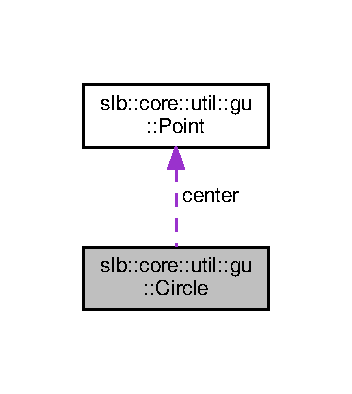
\includegraphics[width=169pt]{structslb_1_1core_1_1util_1_1gu_1_1Circle__coll__graph}
\end{center}
\end{figure}
\subsubsection*{Public Attributes}
\begin{DoxyCompactItemize}
\item 
\hyperlink{structslb_1_1core_1_1util_1_1gu_1_1Point}{Point} \hyperlink{structslb_1_1core_1_1util_1_1gu_1_1Circle_a380fc0b0f6d0d67f65dc68d609905a34}{center}\hypertarget{structslb_1_1core_1_1util_1_1gu_1_1Circle_a380fc0b0f6d0d67f65dc68d609905a34}{}\label{structslb_1_1core_1_1util_1_1gu_1_1Circle_a380fc0b0f6d0d67f65dc68d609905a34}

\begin{DoxyCompactList}\small\item\em The center. \end{DoxyCompactList}\item 
double \hyperlink{structslb_1_1core_1_1util_1_1gu_1_1Circle_a9ed180ddc28350dd5ac91983dbf132ab}{r}\hypertarget{structslb_1_1core_1_1util_1_1gu_1_1Circle_a9ed180ddc28350dd5ac91983dbf132ab}{}\label{structslb_1_1core_1_1util_1_1gu_1_1Circle_a9ed180ddc28350dd5ac91983dbf132ab}

\begin{DoxyCompactList}\small\item\em The radius. \end{DoxyCompactList}\end{DoxyCompactItemize}


\subsubsection{Detailed Description}
The circle. 

Definition at line 19 of file geometry.\+h.



The documentation for this struct was generated from the following file\+:\begin{DoxyCompactItemize}
\item 
core/util/graphics/geometry.\+h\end{DoxyCompactItemize}

\hypertarget{structslb_1_1ext_1_1event_1_1Closed}{}\subsection{slb\+:\+:ext\+:\+:event\+:\+:Closed$<$ Node $>$ Struct Template Reference}
\label{structslb_1_1ext_1_1event_1_1Closed}\index{slb\+::ext\+::event\+::\+Closed$<$ Node $>$@{slb\+::ext\+::event\+::\+Closed$<$ Node $>$}}


Event that visualizes having closed a node.  




{\ttfamily \#include $<$events.\+h$>$}



Inheritance diagram for slb\+:\+:ext\+:\+:event\+:\+:Closed$<$ Node $>$\+:\nopagebreak
\begin{figure}[H]
\begin{center}
\leavevmode
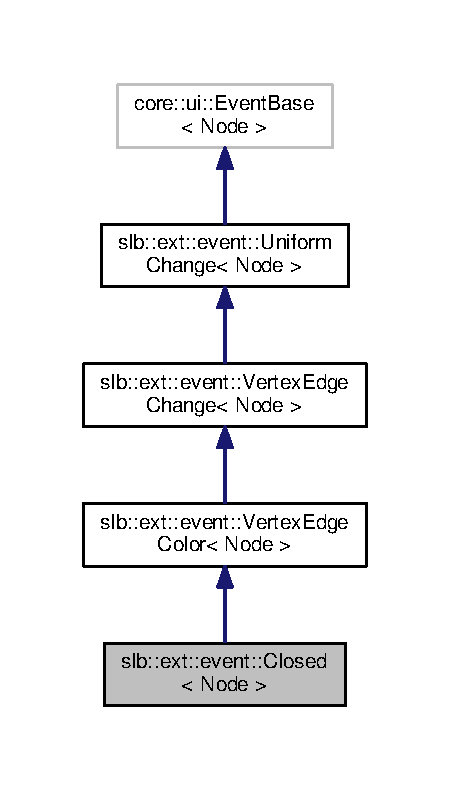
\includegraphics[width=216pt]{structslb_1_1ext_1_1event_1_1Closed__inherit__graph}
\end{center}
\end{figure}


Collaboration diagram for slb\+:\+:ext\+:\+:event\+:\+:Closed$<$ Node $>$\+:\nopagebreak
\begin{figure}[H]
\begin{center}
\leavevmode
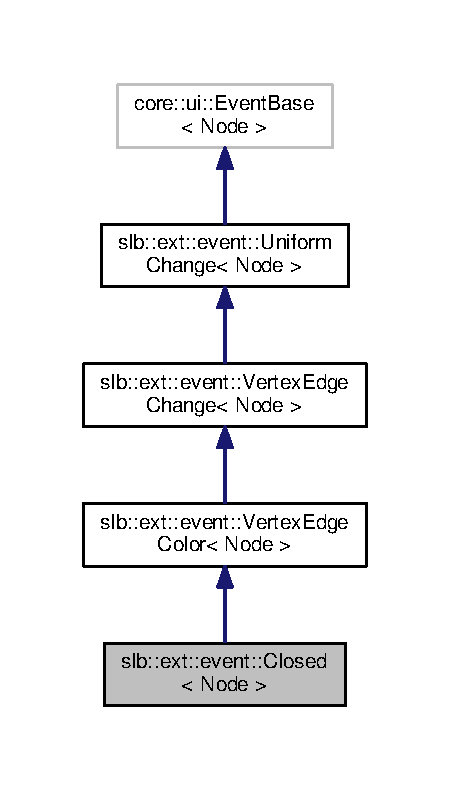
\includegraphics[width=216pt]{structslb_1_1ext_1_1event_1_1Closed__coll__graph}
\end{center}
\end{figure}
\subsubsection*{Private Member Functions}
\begin{DoxyCompactItemize}
\item 
virtual Color \hyperlink{structslb_1_1ext_1_1event_1_1Closed_a481066c0af982217bc6de618cfe48ee5}{color} () const override
\begin{DoxyCompactList}\small\item\em Returns the new color of both the vertex of the state graph corresponding to the state associated with the event and the edge by which the search algorithm arrived to this state. \end{DoxyCompactList}\item 
std\+::string \hyperlink{structslb_1_1ext_1_1event_1_1Closed_af3366063cd8e6c3c6f92497888588331}{event\+Str} () const override
\begin{DoxyCompactList}\small\item\em Returns the string describing the event. This string is displayed in the log window. \end{DoxyCompactList}\end{DoxyCompactItemize}
\subsubsection*{Additional Inherited Members}


\subsubsection{Detailed Description}
\subsubsection*{template$<$class Node = S\+L\+B\+\_\+\+N\+O\+DE$>$\\*
struct slb\+::ext\+::event\+::\+Closed$<$ Node $>$}

Event that visualizes having closed a node. 


\begin{DoxyTemplParams}{Template Parameters}
{\em Node} & The search node type. \\
\hline
\end{DoxyTemplParams}


Definition at line 239 of file events.\+h.



\subsubsection{Member Function Documentation}
\index{slb\+::ext\+::event\+::\+Closed@{slb\+::ext\+::event\+::\+Closed}!color@{color}}
\index{color@{color}!slb\+::ext\+::event\+::\+Closed@{slb\+::ext\+::event\+::\+Closed}}
\paragraph[{\texorpdfstring{color() const override}{color() const override}}]{\setlength{\rightskip}{0pt plus 5cm}template$<$class Node  = S\+L\+B\+\_\+\+N\+O\+DE$>$ virtual Color {\bf slb\+::ext\+::event\+::\+Closed}$<$ Node $>$\+::color (
\begin{DoxyParamCaption}
{}
\end{DoxyParamCaption}
) const\hspace{0.3cm}{\ttfamily [inline]}, {\ttfamily [override]}, {\ttfamily [private]}, {\ttfamily [virtual]}}\hypertarget{structslb_1_1ext_1_1event_1_1Closed_a481066c0af982217bc6de618cfe48ee5}{}\label{structslb_1_1ext_1_1event_1_1Closed_a481066c0af982217bc6de618cfe48ee5}


Returns the new color of both the vertex of the state graph corresponding to the state associated with the event and the edge by which the search algorithm arrived to this state. 

\begin{DoxyReturn}{Returns}
The new color of both the vertex of the state graph corresponding to the state associated with the event and the edge by which the search algorithm arrived to this state. 
\end{DoxyReturn}


Implements \hyperlink{structslb_1_1ext_1_1event_1_1VertexEdgeColor_ac5d0c212a4e807eccbc7082b8834ef77}{slb\+::ext\+::event\+::\+Vertex\+Edge\+Color$<$ Node $>$}.



Definition at line 250 of file events.\+h.

\index{slb\+::ext\+::event\+::\+Closed@{slb\+::ext\+::event\+::\+Closed}!event\+Str@{event\+Str}}
\index{event\+Str@{event\+Str}!slb\+::ext\+::event\+::\+Closed@{slb\+::ext\+::event\+::\+Closed}}
\paragraph[{\texorpdfstring{event\+Str() const override}{eventStr() const override}}]{\setlength{\rightskip}{0pt plus 5cm}template$<$class Node  = S\+L\+B\+\_\+\+N\+O\+DE$>$ std\+::string {\bf slb\+::ext\+::event\+::\+Closed}$<$ Node $>$\+::event\+Str (
\begin{DoxyParamCaption}
{}
\end{DoxyParamCaption}
) const\hspace{0.3cm}{\ttfamily [inline]}, {\ttfamily [override]}, {\ttfamily [private]}}\hypertarget{structslb_1_1ext_1_1event_1_1Closed_af3366063cd8e6c3c6f92497888588331}{}\label{structslb_1_1ext_1_1event_1_1Closed_af3366063cd8e6c3c6f92497888588331}


Returns the string describing the event. This string is displayed in the log window. 

\begin{DoxyReturn}{Returns}
The string describing the event. 
\end{DoxyReturn}


Definition at line 255 of file events.\+h.



The documentation for this struct was generated from the following file\+:\begin{DoxyCompactItemize}
\item 
extensions/events/\hyperlink{events_8h}{events.\+h}\end{DoxyCompactItemize}

\hypertarget{structslb_1_1ext_1_1heuristic_1_1differential_1_1CommandLine}{}\subsection{slb\+:\+:ext\+:\+:heuristic\+:\+:differential\+:\+:Command\+Line Struct Reference}
\label{structslb_1_1ext_1_1heuristic_1_1differential_1_1CommandLine}\index{slb\+::ext\+::heuristic\+::differential\+::\+Command\+Line@{slb\+::ext\+::heuristic\+::differential\+::\+Command\+Line}}


Additions to the command line related to the differential heuristic.  




{\ttfamily \#include $<$differential.\+h$>$}

\subsubsection*{Public Member Functions}
\begin{DoxyCompactItemize}
\item 
int \hyperlink{structslb_1_1ext_1_1heuristic_1_1differential_1_1CommandLine_a17659f8348093e663b2eb1c3fcb986a2}{n\+Pivots} ()
\begin{DoxyCompactList}\small\item\em Returns the number of pivots. \end{DoxyCompactList}\end{DoxyCompactItemize}
\subsubsection*{Protected Member Functions}
\begin{DoxyCompactItemize}
\item 
\hyperlink{structslb_1_1ext_1_1heuristic_1_1differential_1_1CommandLine_aafcf3cdd0b29a6f38d6f79bb63b407e2}{Command\+Line} (T\+C\+L\+A\+P\+::\+Cmd\+Line \&cmd)
\begin{DoxyCompactList}\small\item\em Injects this addition to the command line object. \end{DoxyCompactList}\end{DoxyCompactItemize}
\subsubsection*{Private Attributes}
\begin{DoxyCompactItemize}
\item 
T\+C\+L\+A\+P\+::\+Value\+Arg$<$ int $>$ \hyperlink{structslb_1_1ext_1_1heuristic_1_1differential_1_1CommandLine_ad4bbe83d50e6ec452141b01100e4de48}{n\+Pivots\+\_\+}\hypertarget{structslb_1_1ext_1_1heuristic_1_1differential_1_1CommandLine_ad4bbe83d50e6ec452141b01100e4de48}{}\label{structslb_1_1ext_1_1heuristic_1_1differential_1_1CommandLine_ad4bbe83d50e6ec452141b01100e4de48}

\begin{DoxyCompactList}\small\item\em Command line option for the number of pancakes. \end{DoxyCompactList}\end{DoxyCompactItemize}


\subsubsection{Detailed Description}
Additions to the command line related to the differential heuristic. 

Definition at line 20 of file differential.\+h.



\subsubsection{Constructor \& Destructor Documentation}
\index{slb\+::ext\+::heuristic\+::differential\+::\+Command\+Line@{slb\+::ext\+::heuristic\+::differential\+::\+Command\+Line}!Command\+Line@{Command\+Line}}
\index{Command\+Line@{Command\+Line}!slb\+::ext\+::heuristic\+::differential\+::\+Command\+Line@{slb\+::ext\+::heuristic\+::differential\+::\+Command\+Line}}
\paragraph[{\texorpdfstring{Command\+Line(\+T\+C\+L\+A\+P\+::\+Cmd\+Line \&cmd)}{CommandLine(TCLAP::CmdLine &cmd)}}]{\setlength{\rightskip}{0pt plus 5cm}slb\+::ext\+::heuristic\+::differential\+::\+Command\+Line\+::\+Command\+Line (
\begin{DoxyParamCaption}
\item[{T\+C\+L\+A\+P\+::\+Cmd\+Line \&}]{cmd}
\end{DoxyParamCaption}
)\hspace{0.3cm}{\ttfamily [inline]}, {\ttfamily [protected]}}\hypertarget{structslb_1_1ext_1_1heuristic_1_1differential_1_1CommandLine_aafcf3cdd0b29a6f38d6f79bb63b407e2}{}\label{structslb_1_1ext_1_1heuristic_1_1differential_1_1CommandLine_aafcf3cdd0b29a6f38d6f79bb63b407e2}


Injects this addition to the command line object. 


\begin{DoxyParams}{Parameters}
{\em cmd} & The command-\/line object. \\
\hline
\end{DoxyParams}


Definition at line 32 of file differential.\+h.



\subsubsection{Member Function Documentation}
\index{slb\+::ext\+::heuristic\+::differential\+::\+Command\+Line@{slb\+::ext\+::heuristic\+::differential\+::\+Command\+Line}!n\+Pivots@{n\+Pivots}}
\index{n\+Pivots@{n\+Pivots}!slb\+::ext\+::heuristic\+::differential\+::\+Command\+Line@{slb\+::ext\+::heuristic\+::differential\+::\+Command\+Line}}
\paragraph[{\texorpdfstring{n\+Pivots()}{nPivots()}}]{\setlength{\rightskip}{0pt plus 5cm}int slb\+::ext\+::heuristic\+::differential\+::\+Command\+Line\+::n\+Pivots (
\begin{DoxyParamCaption}
{}
\end{DoxyParamCaption}
)\hspace{0.3cm}{\ttfamily [inline]}}\hypertarget{structslb_1_1ext_1_1heuristic_1_1differential_1_1CommandLine_a17659f8348093e663b2eb1c3fcb986a2}{}\label{structslb_1_1ext_1_1heuristic_1_1differential_1_1CommandLine_a17659f8348093e663b2eb1c3fcb986a2}


Returns the number of pivots. 

\begin{DoxyReturn}{Returns}
The number of pivots. 
\end{DoxyReturn}


Definition at line 23 of file differential.\+h.



The documentation for this struct was generated from the following file\+:\begin{DoxyCompactItemize}
\item 
extensions/heuristics/differential/\hyperlink{differential_8h}{differential.\+h}\end{DoxyCompactItemize}

\hypertarget{structslb_1_1core_1_1commandLine_1_1CommandLine}{}\subsection{slb\+:\+:core\+:\+:command\+Line\+:\+:Command\+Line$<$ Additions $>$ Struct Template Reference}
\label{structslb_1_1core_1_1commandLine_1_1CommandLine}\index{slb\+::core\+::command\+Line\+::\+Command\+Line$<$ Additions $>$@{slb\+::core\+::command\+Line\+::\+Command\+Line$<$ Additions $>$}}


Class handling the command line. It is singleton. The command line would usually be accessed from the other code using the \hyperlink{command__line_8h_a0a5ceb9ceb914e08d345410b561cb37a}{C\+MD} macro.  




{\ttfamily \#include $<$command\+\_\+line.\+h$>$}



Inheritance diagram for slb\+:\+:core\+:\+:command\+Line\+:\+:Command\+Line$<$ Additions $>$\+:\nopagebreak
\begin{figure}[H]
\begin{center}
\leavevmode
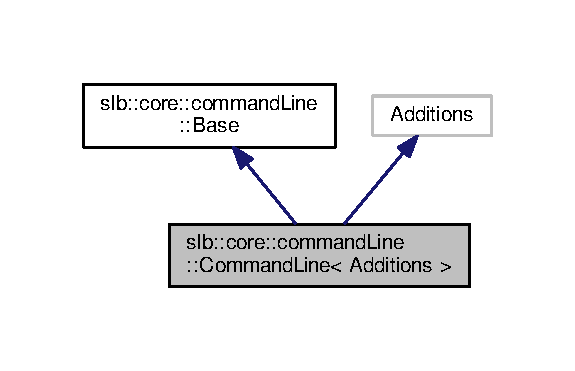
\includegraphics[width=276pt]{structslb_1_1core_1_1commandLine_1_1CommandLine__inherit__graph}
\end{center}
\end{figure}


Collaboration diagram for slb\+:\+:core\+:\+:command\+Line\+:\+:Command\+Line$<$ Additions $>$\+:\nopagebreak
\begin{figure}[H]
\begin{center}
\leavevmode
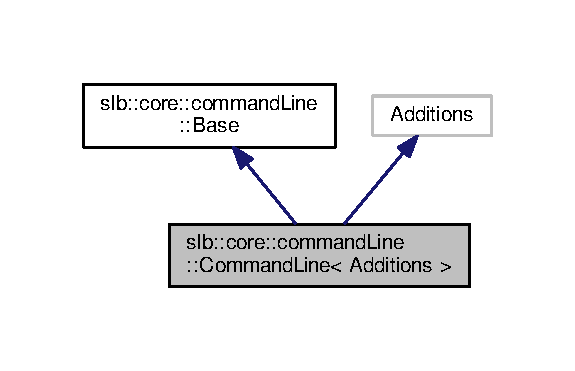
\includegraphics[width=276pt]{structslb_1_1core_1_1commandLine_1_1CommandLine__coll__graph}
\end{center}
\end{figure}
\subsubsection*{Public Member Functions}
\begin{DoxyCompactItemize}
\item 
std\+::string \hyperlink{structslb_1_1core_1_1commandLine_1_1CommandLine_a409b982608d4f5b33db36dd951be94aa}{instances\+File\+Name} ()
\begin{DoxyCompactList}\small\item\em Returns the name of file from which problem instances are to be read. \end{DoxyCompactList}\item 
bool \hyperlink{structslb_1_1core_1_1commandLine_1_1CommandLine_a722e8598fd3bacf7b7c043570761f505}{space\+Init\+File\+Name\+\_\+is\+Set} ()
\begin{DoxyCompactList}\small\item\em Returns {\ttfamily true} if an explicit domain is to be read from a file and {\ttfamily false} otherwise. \end{DoxyCompactList}\item 
std\+::string \hyperlink{structslb_1_1core_1_1commandLine_1_1CommandLine_a516622ca0df35c3cebc2f58d9cf8f6cc}{space\+Init\+File\+Name} ()
\begin{DoxyCompactList}\small\item\em Returns the name of the file from which the explicit domain is to be read. \end{DoxyCompactList}\item 
int \hyperlink{structslb_1_1core_1_1commandLine_1_1CommandLine_a6158f28b2570a978155cc404f6f7d053}{n\+Instances} ()
\begin{DoxyCompactList}\small\item\em Returns the number of problem instances. \end{DoxyCompactList}\item 
int \hyperlink{structslb_1_1core_1_1commandLine_1_1CommandLine_a898532baa7038c47f17de8390d50459f}{visualize\+Instance} ()
\begin{DoxyCompactList}\small\item\em Returns the instance number for which the visualizer is to be run. If visualization is not to be performed, the function returns -\/1. \end{DoxyCompactList}\item 
int \hyperlink{structslb_1_1core_1_1commandLine_1_1CommandLine_a2ae1702ab278a15945e753b3097fcad4}{n\+Starts} (char mode)
\begin{DoxyCompactList}\small\item\em Returns the number of start states in a problem instance. \end{DoxyCompactList}\item 
int \hyperlink{structslb_1_1core_1_1commandLine_1_1CommandLine_a062e26ee110941ffbe598f13313b758c}{n\+Goals} (char mode)
\begin{DoxyCompactList}\small\item\em Returns the number of goal states in a problem instance. \end{DoxyCompactList}\item 
bool \hyperlink{structslb_1_1core_1_1commandLine_1_1CommandLine_a8f2cd242e85739a4aef2733755811fa7}{default\+Goal} ()
\begin{DoxyCompactList}\small\item\em Returns {\ttfamily true} if the first goal in the instance being created should be the default state of the domain and {\ttfamily false} otherwise. \end{DoxyCompactList}\item 
bool \hyperlink{structslb_1_1core_1_1commandLine_1_1CommandLine_aba20650577b010f9699c127e258821c3}{per\+Instance} ()
\begin{DoxyCompactList}\small\item\em Returns {\ttfamily true} if per-\/problem-\/instance statistics are to appear on the output and {\ttfamily false} otherwise. \end{DoxyCompactList}\item 
bool \hyperlink{structslb_1_1core_1_1commandLine_1_1CommandLine_a49a9a1dc9794bbabde1247dfdf056823}{hide\+Title} ()
\begin{DoxyCompactList}\small\item\em Returns {\ttfamily true} if the title row should not appear on the output and {\ttfamily false} otherwise. \end{DoxyCompactList}\item 
std\+::string \hyperlink{structslb_1_1core_1_1commandLine_1_1CommandLine_aea4d54aee80abe312965b0508751b925}{prefix\+Title} ()
\begin{DoxyCompactList}\small\item\em Returns the string with which the title row is to be prefixed. \end{DoxyCompactList}\item 
std\+::string \hyperlink{structslb_1_1core_1_1commandLine_1_1CommandLine_a0fde6d0c2ba0719bb6dacaab612c872b}{prefix\+Data} ()
\begin{DoxyCompactList}\small\item\em Returns the string with which each data row is to be prefixed. \end{DoxyCompactList}\end{DoxyCompactItemize}
\subsubsection*{Static Public Member Functions}
\begin{DoxyCompactItemize}
\item 
static \hyperlink{structslb_1_1core_1_1commandLine_1_1CommandLine}{Command\+Line} \& \hyperlink{structslb_1_1core_1_1commandLine_1_1CommandLine_a297df54d1f330d491717b487968b0fc5}{instance} (int argc=0, char $\ast$$\ast$argv=nullptr)
\begin{DoxyCompactList}\small\item\em Access to the command line object. When this method is called for the first time, it should be called with proper (i.\+e. not default) {\ttfamily argc} and {\ttfamily argv}. \end{DoxyCompactList}\end{DoxyCompactItemize}
\subsubsection*{Private Member Functions}
\begin{DoxyCompactItemize}
\item 
\hyperlink{structslb_1_1core_1_1commandLine_1_1CommandLine_a483a8ee633d26d4e6423387d5f81daf7}{Command\+Line} (int argc, char $\ast$$\ast$argv)
\begin{DoxyCompactList}\small\item\em Initializes the command line given {\ttfamily argc} and {\ttfamily argv}. \end{DoxyCompactList}\end{DoxyCompactItemize}
\subsubsection*{Private Attributes}
\begin{DoxyCompactItemize}
\item 
T\+C\+L\+A\+P\+::\+Value\+Arg$<$ std\+::string $>$ \hyperlink{structslb_1_1core_1_1commandLine_1_1CommandLine_aae80eb58b58985870f186e80d7b16f0c}{instances\+File\+Name\+\_\+}\hypertarget{structslb_1_1core_1_1commandLine_1_1CommandLine_aae80eb58b58985870f186e80d7b16f0c}{}\label{structslb_1_1core_1_1commandLine_1_1CommandLine_aae80eb58b58985870f186e80d7b16f0c}

\begin{DoxyCompactList}\small\item\em Command line option for the name of file from which problem instances are to be read. \end{DoxyCompactList}\item 
T\+C\+L\+A\+P\+::\+Value\+Arg$<$ std\+::string $>$ \hyperlink{structslb_1_1core_1_1commandLine_1_1CommandLine_a2d5e9932ad4c70e62f1a8f5760665880}{space\+Init\+File\+Name\+\_\+}\hypertarget{structslb_1_1core_1_1commandLine_1_1CommandLine_a2d5e9932ad4c70e62f1a8f5760665880}{}\label{structslb_1_1core_1_1commandLine_1_1CommandLine_a2d5e9932ad4c70e62f1a8f5760665880}

\begin{DoxyCompactList}\small\item\em Command line option for the name of the file from which the explicit domain is to be read. \end{DoxyCompactList}\item 
T\+C\+L\+A\+P\+::\+Value\+Arg$<$ int $>$ \hyperlink{structslb_1_1core_1_1commandLine_1_1CommandLine_a45634f339b37747bcc19ce6c9e35d321}{n\+Instances\+\_\+}\hypertarget{structslb_1_1core_1_1commandLine_1_1CommandLine_a45634f339b37747bcc19ce6c9e35d321}{}\label{structslb_1_1core_1_1commandLine_1_1CommandLine_a45634f339b37747bcc19ce6c9e35d321}

\begin{DoxyCompactList}\small\item\em Command line option for the number of problem instances. \end{DoxyCompactList}\item 
T\+C\+L\+A\+P\+::\+Value\+Arg$<$ int $>$ \hyperlink{structslb_1_1core_1_1commandLine_1_1CommandLine_a4ada16371a5e3052b75b91658613f283}{visualize\+\_\+}\hypertarget{structslb_1_1core_1_1commandLine_1_1CommandLine_a4ada16371a5e3052b75b91658613f283}{}\label{structslb_1_1core_1_1commandLine_1_1CommandLine_a4ada16371a5e3052b75b91658613f283}

\begin{DoxyCompactList}\small\item\em Command line option for the instance number for which the visualizer is to be run. It would hold -\/1 if visualization is not to be performed. \end{DoxyCompactList}\item 
T\+C\+L\+A\+P\+::\+Value\+Arg$<$ int $>$ \hyperlink{structslb_1_1core_1_1commandLine_1_1CommandLine_af848807b96ecf4560989abb9b78bfdf5}{n\+Starts\+\_\+}\hypertarget{structslb_1_1core_1_1commandLine_1_1CommandLine_af848807b96ecf4560989abb9b78bfdf5}{}\label{structslb_1_1core_1_1commandLine_1_1CommandLine_af848807b96ecf4560989abb9b78bfdf5}

\begin{DoxyCompactList}\small\item\em Command line option for the number of start states in a problem instance. \end{DoxyCompactList}\item 
T\+C\+L\+A\+P\+::\+Value\+Arg$<$ int $>$ \hyperlink{structslb_1_1core_1_1commandLine_1_1CommandLine_a68720f2ac1005479c84cc6cd681696e3}{n\+Goals\+\_\+}\hypertarget{structslb_1_1core_1_1commandLine_1_1CommandLine_a68720f2ac1005479c84cc6cd681696e3}{}\label{structslb_1_1core_1_1commandLine_1_1CommandLine_a68720f2ac1005479c84cc6cd681696e3}

\begin{DoxyCompactList}\small\item\em Command line option for the number of goal states in a problem instance. \end{DoxyCompactList}\item 
T\+C\+L\+A\+P\+::\+Switch\+Arg \hyperlink{structslb_1_1core_1_1commandLine_1_1CommandLine_a7157af3d110066e82e11493e93e37050}{default\+Goal\+\_\+}\hypertarget{structslb_1_1core_1_1commandLine_1_1CommandLine_a7157af3d110066e82e11493e93e37050}{}\label{structslb_1_1core_1_1commandLine_1_1CommandLine_a7157af3d110066e82e11493e93e37050}

\begin{DoxyCompactList}\small\item\em Command line option for the switch showing whether the first goal in the instance being created should be the default state of the domain. \end{DoxyCompactList}\item 
T\+C\+L\+A\+P\+::\+Switch\+Arg \hyperlink{structslb_1_1core_1_1commandLine_1_1CommandLine_a7f35a809f1c1b6ccbf080d2cb6109a22}{per\+Instance\+\_\+}\hypertarget{structslb_1_1core_1_1commandLine_1_1CommandLine_a7f35a809f1c1b6ccbf080d2cb6109a22}{}\label{structslb_1_1core_1_1commandLine_1_1CommandLine_a7f35a809f1c1b6ccbf080d2cb6109a22}

\begin{DoxyCompactList}\small\item\em Command line option for the switch showing whether per-\/problem-\/instance statistics are to appear on the output. \end{DoxyCompactList}\item 
T\+C\+L\+A\+P\+::\+Switch\+Arg \hyperlink{structslb_1_1core_1_1commandLine_1_1CommandLine_aafd86c8565922240a0e7adf3040b8fa1}{hide\+Title\+\_\+}\hypertarget{structslb_1_1core_1_1commandLine_1_1CommandLine_aafd86c8565922240a0e7adf3040b8fa1}{}\label{structslb_1_1core_1_1commandLine_1_1CommandLine_aafd86c8565922240a0e7adf3040b8fa1}

\begin{DoxyCompactList}\small\item\em Command line option for the switch showing whether the title row is to appear on the output. \end{DoxyCompactList}\item 
T\+C\+L\+A\+P\+::\+Value\+Arg$<$ std\+::string $>$ \hyperlink{structslb_1_1core_1_1commandLine_1_1CommandLine_a2fd89f93aa659f5f0ddfafc9711f15a0}{prefix\+Title\+\_\+}\hypertarget{structslb_1_1core_1_1commandLine_1_1CommandLine_a2fd89f93aa659f5f0ddfafc9711f15a0}{}\label{structslb_1_1core_1_1commandLine_1_1CommandLine_a2fd89f93aa659f5f0ddfafc9711f15a0}

\begin{DoxyCompactList}\small\item\em Command line option for the string with which the title row is to be prefixed. \end{DoxyCompactList}\item 
T\+C\+L\+A\+P\+::\+Value\+Arg$<$ std\+::string $>$ \hyperlink{structslb_1_1core_1_1commandLine_1_1CommandLine_af251cbd553a5150c57dcfb25c1bc3a8c}{prefix\+Data\+\_\+}\hypertarget{structslb_1_1core_1_1commandLine_1_1CommandLine_af251cbd553a5150c57dcfb25c1bc3a8c}{}\label{structslb_1_1core_1_1commandLine_1_1CommandLine_af251cbd553a5150c57dcfb25c1bc3a8c}

\begin{DoxyCompactList}\small\item\em Command line option for the string with which each data row is to be prefixed. \end{DoxyCompactList}\end{DoxyCompactItemize}
\subsubsection*{Additional Inherited Members}


\subsubsection{Detailed Description}
\subsubsection*{template$<$class Additions = S\+L\+B\+\_\+\+C\+M\+D\+\_\+\+L\+I\+N\+E\+\_\+\+A\+DD$>$\\*
struct slb\+::core\+::command\+Line\+::\+Command\+Line$<$ Additions $>$}

Class handling the command line. It is singleton. The command line would usually be accessed from the other code using the \hyperlink{command__line_8h_a0a5ceb9ceb914e08d345410b561cb37a}{C\+MD} macro. 


\begin{DoxyTemplParams}{Template Parameters}
{\em Additions} & Command line additions. \\
\hline
\end{DoxyTemplParams}


Definition at line 51 of file command\+\_\+line.\+h.



\subsubsection{Constructor \& Destructor Documentation}
\index{slb\+::core\+::command\+Line\+::\+Command\+Line@{slb\+::core\+::command\+Line\+::\+Command\+Line}!Command\+Line@{Command\+Line}}
\index{Command\+Line@{Command\+Line}!slb\+::core\+::command\+Line\+::\+Command\+Line@{slb\+::core\+::command\+Line\+::\+Command\+Line}}
\paragraph[{\texorpdfstring{Command\+Line(int argc, char $\ast$$\ast$argv)}{CommandLine(int argc, char **argv)}}]{\setlength{\rightskip}{0pt plus 5cm}template$<$class Additions  = S\+L\+B\+\_\+\+C\+M\+D\+\_\+\+L\+I\+N\+E\+\_\+\+A\+DD$>$ {\bf slb\+::core\+::command\+Line\+::\+Command\+Line}$<$ Additions $>$\+::{\bf Command\+Line} (
\begin{DoxyParamCaption}
\item[{int}]{argc, }
\item[{char $\ast$$\ast$}]{argv}
\end{DoxyParamCaption}
)\hspace{0.3cm}{\ttfamily [inline]}, {\ttfamily [private]}}\hypertarget{structslb_1_1core_1_1commandLine_1_1CommandLine_a483a8ee633d26d4e6423387d5f81daf7}{}\label{structslb_1_1core_1_1commandLine_1_1CommandLine_a483a8ee633d26d4e6423387d5f81daf7}


Initializes the command line given {\ttfamily argc} and {\ttfamily argv}. 


\begin{DoxyParams}{Parameters}
{\em argc} & Number of command line arguments. \\
\hline
{\em argv} & The command line arguments. \\
\hline
\end{DoxyParams}


Definition at line 181 of file command\+\_\+line.\+h.



\subsubsection{Member Function Documentation}
\index{slb\+::core\+::command\+Line\+::\+Command\+Line@{slb\+::core\+::command\+Line\+::\+Command\+Line}!default\+Goal@{default\+Goal}}
\index{default\+Goal@{default\+Goal}!slb\+::core\+::command\+Line\+::\+Command\+Line@{slb\+::core\+::command\+Line\+::\+Command\+Line}}
\paragraph[{\texorpdfstring{default\+Goal()}{defaultGoal()}}]{\setlength{\rightskip}{0pt plus 5cm}template$<$class Additions  = S\+L\+B\+\_\+\+C\+M\+D\+\_\+\+L\+I\+N\+E\+\_\+\+A\+DD$>$ bool {\bf slb\+::core\+::command\+Line\+::\+Command\+Line}$<$ Additions $>$\+::default\+Goal (
\begin{DoxyParamCaption}
{}
\end{DoxyParamCaption}
)\hspace{0.3cm}{\ttfamily [inline]}}\hypertarget{structslb_1_1core_1_1commandLine_1_1CommandLine_a8f2cd242e85739a4aef2733755811fa7}{}\label{structslb_1_1core_1_1commandLine_1_1CommandLine_a8f2cd242e85739a4aef2733755811fa7}


Returns {\ttfamily true} if the first goal in the instance being created should be the default state of the domain and {\ttfamily false} otherwise. 

\begin{DoxyReturn}{Returns}
{\ttfamily true} the first goal in the instance being created should be the default state of the domain and {\ttfamily false} otherwise. 
\end{DoxyReturn}


Definition at line 112 of file command\+\_\+line.\+h.

\index{slb\+::core\+::command\+Line\+::\+Command\+Line@{slb\+::core\+::command\+Line\+::\+Command\+Line}!hide\+Title@{hide\+Title}}
\index{hide\+Title@{hide\+Title}!slb\+::core\+::command\+Line\+::\+Command\+Line@{slb\+::core\+::command\+Line\+::\+Command\+Line}}
\paragraph[{\texorpdfstring{hide\+Title()}{hideTitle()}}]{\setlength{\rightskip}{0pt plus 5cm}template$<$class Additions  = S\+L\+B\+\_\+\+C\+M\+D\+\_\+\+L\+I\+N\+E\+\_\+\+A\+DD$>$ bool {\bf slb\+::core\+::command\+Line\+::\+Command\+Line}$<$ Additions $>$\+::hide\+Title (
\begin{DoxyParamCaption}
{}
\end{DoxyParamCaption}
)\hspace{0.3cm}{\ttfamily [inline]}}\hypertarget{structslb_1_1core_1_1commandLine_1_1CommandLine_a49a9a1dc9794bbabde1247dfdf056823}{}\label{structslb_1_1core_1_1commandLine_1_1CommandLine_a49a9a1dc9794bbabde1247dfdf056823}


Returns {\ttfamily true} if the title row should not appear on the output and {\ttfamily false} otherwise. 

\begin{DoxyReturn}{Returns}
{\ttfamily true} if the title row should not appear on the output and {\ttfamily false} otherwise. 
\end{DoxyReturn}


Definition at line 124 of file command\+\_\+line.\+h.

\index{slb\+::core\+::command\+Line\+::\+Command\+Line@{slb\+::core\+::command\+Line\+::\+Command\+Line}!instance@{instance}}
\index{instance@{instance}!slb\+::core\+::command\+Line\+::\+Command\+Line@{slb\+::core\+::command\+Line\+::\+Command\+Line}}
\paragraph[{\texorpdfstring{instance(int argc=0, char $\ast$$\ast$argv=nullptr)}{instance(int argc=0, char **argv=nullptr)}}]{\setlength{\rightskip}{0pt plus 5cm}template$<$class Additions  = S\+L\+B\+\_\+\+C\+M\+D\+\_\+\+L\+I\+N\+E\+\_\+\+A\+DD$>$ static {\bf Command\+Line}\& {\bf slb\+::core\+::command\+Line\+::\+Command\+Line}$<$ Additions $>$\+::instance (
\begin{DoxyParamCaption}
\item[{int}]{argc = {\ttfamily 0}, }
\item[{char $\ast$$\ast$}]{argv = {\ttfamily nullptr}}
\end{DoxyParamCaption}
)\hspace{0.3cm}{\ttfamily [inline]}, {\ttfamily [static]}}\hypertarget{structslb_1_1core_1_1commandLine_1_1CommandLine_a297df54d1f330d491717b487968b0fc5}{}\label{structslb_1_1core_1_1commandLine_1_1CommandLine_a297df54d1f330d491717b487968b0fc5}


Access to the command line object. When this method is called for the first time, it should be called with proper (i.\+e. not default) {\ttfamily argc} and {\ttfamily argv}. 


\begin{DoxyParams}{Parameters}
{\em argc} & Number of command line arguments. \\
\hline
{\em argv} & The command line arguments. \\
\hline
\end{DoxyParams}
\begin{DoxyReturn}{Returns}
The command line object. 
\end{DoxyReturn}


Definition at line 58 of file command\+\_\+line.\+h.

\index{slb\+::core\+::command\+Line\+::\+Command\+Line@{slb\+::core\+::command\+Line\+::\+Command\+Line}!instances\+File\+Name@{instances\+File\+Name}}
\index{instances\+File\+Name@{instances\+File\+Name}!slb\+::core\+::command\+Line\+::\+Command\+Line@{slb\+::core\+::command\+Line\+::\+Command\+Line}}
\paragraph[{\texorpdfstring{instances\+File\+Name()}{instancesFileName()}}]{\setlength{\rightskip}{0pt plus 5cm}template$<$class Additions  = S\+L\+B\+\_\+\+C\+M\+D\+\_\+\+L\+I\+N\+E\+\_\+\+A\+DD$>$ std\+::string {\bf slb\+::core\+::command\+Line\+::\+Command\+Line}$<$ Additions $>$\+::instances\+File\+Name (
\begin{DoxyParamCaption}
{}
\end{DoxyParamCaption}
)\hspace{0.3cm}{\ttfamily [inline]}}\hypertarget{structslb_1_1core_1_1commandLine_1_1CommandLine_a409b982608d4f5b33db36dd951be94aa}{}\label{structslb_1_1core_1_1commandLine_1_1CommandLine_a409b982608d4f5b33db36dd951be94aa}


Returns the name of file from which problem instances are to be read. 

\begin{DoxyReturn}{Returns}
The name of file from which problem instances are to be read. 
\end{DoxyReturn}


Definition at line 65 of file command\+\_\+line.\+h.

\index{slb\+::core\+::command\+Line\+::\+Command\+Line@{slb\+::core\+::command\+Line\+::\+Command\+Line}!n\+Goals@{n\+Goals}}
\index{n\+Goals@{n\+Goals}!slb\+::core\+::command\+Line\+::\+Command\+Line@{slb\+::core\+::command\+Line\+::\+Command\+Line}}
\paragraph[{\texorpdfstring{n\+Goals(char mode)}{nGoals(char mode)}}]{\setlength{\rightskip}{0pt plus 5cm}template$<$class Additions  = S\+L\+B\+\_\+\+C\+M\+D\+\_\+\+L\+I\+N\+E\+\_\+\+A\+DD$>$ int {\bf slb\+::core\+::command\+Line\+::\+Command\+Line}$<$ Additions $>$\+::n\+Goals (
\begin{DoxyParamCaption}
\item[{char}]{mode}
\end{DoxyParamCaption}
)\hspace{0.3cm}{\ttfamily [inline]}}\hypertarget{structslb_1_1core_1_1commandLine_1_1CommandLine_a062e26ee110941ffbe598f13313b758c}{}\label{structslb_1_1core_1_1commandLine_1_1CommandLine_a062e26ee110941ffbe598f13313b758c}


Returns the number of goal states in a problem instance. 


\begin{DoxyParams}{Parameters}
{\em mode} & {\ttfamily \textquotesingle{}r\textquotesingle{}} or \textquotesingle{}w\textquotesingle{} depending on whether the problem instances file is being read or written, respectively. \\
\hline
\end{DoxyParams}
\begin{DoxyReturn}{Returns}
The number of goal states in a problem instance. 
\end{DoxyReturn}


Definition at line 103 of file command\+\_\+line.\+h.

\index{slb\+::core\+::command\+Line\+::\+Command\+Line@{slb\+::core\+::command\+Line\+::\+Command\+Line}!n\+Instances@{n\+Instances}}
\index{n\+Instances@{n\+Instances}!slb\+::core\+::command\+Line\+::\+Command\+Line@{slb\+::core\+::command\+Line\+::\+Command\+Line}}
\paragraph[{\texorpdfstring{n\+Instances()}{nInstances()}}]{\setlength{\rightskip}{0pt plus 5cm}template$<$class Additions  = S\+L\+B\+\_\+\+C\+M\+D\+\_\+\+L\+I\+N\+E\+\_\+\+A\+DD$>$ int {\bf slb\+::core\+::command\+Line\+::\+Command\+Line}$<$ Additions $>$\+::n\+Instances (
\begin{DoxyParamCaption}
{}
\end{DoxyParamCaption}
)\hspace{0.3cm}{\ttfamily [inline]}}\hypertarget{structslb_1_1core_1_1commandLine_1_1CommandLine_a6158f28b2570a978155cc404f6f7d053}{}\label{structslb_1_1core_1_1commandLine_1_1CommandLine_a6158f28b2570a978155cc404f6f7d053}


Returns the number of problem instances. 

\begin{DoxyReturn}{Returns}
The number of problem instances. 
\end{DoxyReturn}


Definition at line 81 of file command\+\_\+line.\+h.

\index{slb\+::core\+::command\+Line\+::\+Command\+Line@{slb\+::core\+::command\+Line\+::\+Command\+Line}!n\+Starts@{n\+Starts}}
\index{n\+Starts@{n\+Starts}!slb\+::core\+::command\+Line\+::\+Command\+Line@{slb\+::core\+::command\+Line\+::\+Command\+Line}}
\paragraph[{\texorpdfstring{n\+Starts(char mode)}{nStarts(char mode)}}]{\setlength{\rightskip}{0pt plus 5cm}template$<$class Additions  = S\+L\+B\+\_\+\+C\+M\+D\+\_\+\+L\+I\+N\+E\+\_\+\+A\+DD$>$ int {\bf slb\+::core\+::command\+Line\+::\+Command\+Line}$<$ Additions $>$\+::n\+Starts (
\begin{DoxyParamCaption}
\item[{char}]{mode}
\end{DoxyParamCaption}
)\hspace{0.3cm}{\ttfamily [inline]}}\hypertarget{structslb_1_1core_1_1commandLine_1_1CommandLine_a2ae1702ab278a15945e753b3097fcad4}{}\label{structslb_1_1core_1_1commandLine_1_1CommandLine_a2ae1702ab278a15945e753b3097fcad4}


Returns the number of start states in a problem instance. 


\begin{DoxyParams}{Parameters}
{\em mode} & {\ttfamily \textquotesingle{}r\textquotesingle{}} or \textquotesingle{}w\textquotesingle{} depending on whether the problem instances file is being read or written, respectively. \\
\hline
\end{DoxyParams}
\begin{DoxyReturn}{Returns}
The number of start states in a problem instance. 
\end{DoxyReturn}


Definition at line 94 of file command\+\_\+line.\+h.

\index{slb\+::core\+::command\+Line\+::\+Command\+Line@{slb\+::core\+::command\+Line\+::\+Command\+Line}!per\+Instance@{per\+Instance}}
\index{per\+Instance@{per\+Instance}!slb\+::core\+::command\+Line\+::\+Command\+Line@{slb\+::core\+::command\+Line\+::\+Command\+Line}}
\paragraph[{\texorpdfstring{per\+Instance()}{perInstance()}}]{\setlength{\rightskip}{0pt plus 5cm}template$<$class Additions  = S\+L\+B\+\_\+\+C\+M\+D\+\_\+\+L\+I\+N\+E\+\_\+\+A\+DD$>$ bool {\bf slb\+::core\+::command\+Line\+::\+Command\+Line}$<$ Additions $>$\+::per\+Instance (
\begin{DoxyParamCaption}
{}
\end{DoxyParamCaption}
)\hspace{0.3cm}{\ttfamily [inline]}}\hypertarget{structslb_1_1core_1_1commandLine_1_1CommandLine_aba20650577b010f9699c127e258821c3}{}\label{structslb_1_1core_1_1commandLine_1_1CommandLine_aba20650577b010f9699c127e258821c3}


Returns {\ttfamily true} if per-\/problem-\/instance statistics are to appear on the output and {\ttfamily false} otherwise. 

\begin{DoxyReturn}{Returns}
{\ttfamily true} if per-\/problem-\/instance statistics are to appear on the output and {\ttfamily false} otherwise. 
\end{DoxyReturn}


Definition at line 118 of file command\+\_\+line.\+h.

\index{slb\+::core\+::command\+Line\+::\+Command\+Line@{slb\+::core\+::command\+Line\+::\+Command\+Line}!prefix\+Data@{prefix\+Data}}
\index{prefix\+Data@{prefix\+Data}!slb\+::core\+::command\+Line\+::\+Command\+Line@{slb\+::core\+::command\+Line\+::\+Command\+Line}}
\paragraph[{\texorpdfstring{prefix\+Data()}{prefixData()}}]{\setlength{\rightskip}{0pt plus 5cm}template$<$class Additions  = S\+L\+B\+\_\+\+C\+M\+D\+\_\+\+L\+I\+N\+E\+\_\+\+A\+DD$>$ std\+::string {\bf slb\+::core\+::command\+Line\+::\+Command\+Line}$<$ Additions $>$\+::prefix\+Data (
\begin{DoxyParamCaption}
{}
\end{DoxyParamCaption}
)\hspace{0.3cm}{\ttfamily [inline]}}\hypertarget{structslb_1_1core_1_1commandLine_1_1CommandLine_a0fde6d0c2ba0719bb6dacaab612c872b}{}\label{structslb_1_1core_1_1commandLine_1_1CommandLine_a0fde6d0c2ba0719bb6dacaab612c872b}


Returns the string with which each data row is to be prefixed. 

\begin{DoxyReturn}{Returns}
The string with which each data row is to be prefixed. 
\end{DoxyReturn}


Definition at line 132 of file command\+\_\+line.\+h.

\index{slb\+::core\+::command\+Line\+::\+Command\+Line@{slb\+::core\+::command\+Line\+::\+Command\+Line}!prefix\+Title@{prefix\+Title}}
\index{prefix\+Title@{prefix\+Title}!slb\+::core\+::command\+Line\+::\+Command\+Line@{slb\+::core\+::command\+Line\+::\+Command\+Line}}
\paragraph[{\texorpdfstring{prefix\+Title()}{prefixTitle()}}]{\setlength{\rightskip}{0pt plus 5cm}template$<$class Additions  = S\+L\+B\+\_\+\+C\+M\+D\+\_\+\+L\+I\+N\+E\+\_\+\+A\+DD$>$ std\+::string {\bf slb\+::core\+::command\+Line\+::\+Command\+Line}$<$ Additions $>$\+::prefix\+Title (
\begin{DoxyParamCaption}
{}
\end{DoxyParamCaption}
)\hspace{0.3cm}{\ttfamily [inline]}}\hypertarget{structslb_1_1core_1_1commandLine_1_1CommandLine_aea4d54aee80abe312965b0508751b925}{}\label{structslb_1_1core_1_1commandLine_1_1CommandLine_aea4d54aee80abe312965b0508751b925}


Returns the string with which the title row is to be prefixed. 

\begin{DoxyReturn}{Returns}
The string with which the title row is to be prefixed. 
\end{DoxyReturn}


Definition at line 128 of file command\+\_\+line.\+h.

\index{slb\+::core\+::command\+Line\+::\+Command\+Line@{slb\+::core\+::command\+Line\+::\+Command\+Line}!space\+Init\+File\+Name@{space\+Init\+File\+Name}}
\index{space\+Init\+File\+Name@{space\+Init\+File\+Name}!slb\+::core\+::command\+Line\+::\+Command\+Line@{slb\+::core\+::command\+Line\+::\+Command\+Line}}
\paragraph[{\texorpdfstring{space\+Init\+File\+Name()}{spaceInitFileName()}}]{\setlength{\rightskip}{0pt plus 5cm}template$<$class Additions  = S\+L\+B\+\_\+\+C\+M\+D\+\_\+\+L\+I\+N\+E\+\_\+\+A\+DD$>$ std\+::string {\bf slb\+::core\+::command\+Line\+::\+Command\+Line}$<$ Additions $>$\+::space\+Init\+File\+Name (
\begin{DoxyParamCaption}
{}
\end{DoxyParamCaption}
)\hspace{0.3cm}{\ttfamily [inline]}}\hypertarget{structslb_1_1core_1_1commandLine_1_1CommandLine_a516622ca0df35c3cebc2f58d9cf8f6cc}{}\label{structslb_1_1core_1_1commandLine_1_1CommandLine_a516622ca0df35c3cebc2f58d9cf8f6cc}


Returns the name of the file from which the explicit domain is to be read. 

\begin{DoxyReturn}{Returns}
The name of the file from which the explicit domain is to be read. 
\end{DoxyReturn}


Definition at line 77 of file command\+\_\+line.\+h.

\index{slb\+::core\+::command\+Line\+::\+Command\+Line@{slb\+::core\+::command\+Line\+::\+Command\+Line}!space\+Init\+File\+Name\+\_\+is\+Set@{space\+Init\+File\+Name\+\_\+is\+Set}}
\index{space\+Init\+File\+Name\+\_\+is\+Set@{space\+Init\+File\+Name\+\_\+is\+Set}!slb\+::core\+::command\+Line\+::\+Command\+Line@{slb\+::core\+::command\+Line\+::\+Command\+Line}}
\paragraph[{\texorpdfstring{space\+Init\+File\+Name\+\_\+is\+Set()}{spaceInitFileName_isSet()}}]{\setlength{\rightskip}{0pt plus 5cm}template$<$class Additions  = S\+L\+B\+\_\+\+C\+M\+D\+\_\+\+L\+I\+N\+E\+\_\+\+A\+DD$>$ bool {\bf slb\+::core\+::command\+Line\+::\+Command\+Line}$<$ Additions $>$\+::space\+Init\+File\+Name\+\_\+is\+Set (
\begin{DoxyParamCaption}
{}
\end{DoxyParamCaption}
)\hspace{0.3cm}{\ttfamily [inline]}}\hypertarget{structslb_1_1core_1_1commandLine_1_1CommandLine_a722e8598fd3bacf7b7c043570761f505}{}\label{structslb_1_1core_1_1commandLine_1_1CommandLine_a722e8598fd3bacf7b7c043570761f505}


Returns {\ttfamily true} if an explicit domain is to be read from a file and {\ttfamily false} otherwise. 

\begin{DoxyReturn}{Returns}
{\ttfamily true} if an explicit domain is to be read from a file and {\ttfamily false} otherwise. 
\end{DoxyReturn}


Definition at line 71 of file command\+\_\+line.\+h.

\index{slb\+::core\+::command\+Line\+::\+Command\+Line@{slb\+::core\+::command\+Line\+::\+Command\+Line}!visualize\+Instance@{visualize\+Instance}}
\index{visualize\+Instance@{visualize\+Instance}!slb\+::core\+::command\+Line\+::\+Command\+Line@{slb\+::core\+::command\+Line\+::\+Command\+Line}}
\paragraph[{\texorpdfstring{visualize\+Instance()}{visualizeInstance()}}]{\setlength{\rightskip}{0pt plus 5cm}template$<$class Additions  = S\+L\+B\+\_\+\+C\+M\+D\+\_\+\+L\+I\+N\+E\+\_\+\+A\+DD$>$ int {\bf slb\+::core\+::command\+Line\+::\+Command\+Line}$<$ Additions $>$\+::visualize\+Instance (
\begin{DoxyParamCaption}
{}
\end{DoxyParamCaption}
)\hspace{0.3cm}{\ttfamily [inline]}}\hypertarget{structslb_1_1core_1_1commandLine_1_1CommandLine_a898532baa7038c47f17de8390d50459f}{}\label{structslb_1_1core_1_1commandLine_1_1CommandLine_a898532baa7038c47f17de8390d50459f}


Returns the instance number for which the visualizer is to be run. If visualization is not to be performed, the function returns -\/1. 

\begin{DoxyReturn}{Returns}
The instance number for which the visualizer is to be run or -\/1 if visualization is not to be performed. 
\end{DoxyReturn}


Definition at line 88 of file command\+\_\+line.\+h.



The documentation for this struct was generated from the following file\+:\begin{DoxyCompactItemize}
\item 
core/\hyperlink{command__line_8h}{command\+\_\+line.\+h}\end{DoxyCompactItemize}

\hypertarget{structslb_1_1ext_1_1domain_1_1pancake_1_1CommandLine}{}\subsection{slb\+:\+:ext\+:\+:domain\+:\+:pancake\+:\+:Command\+Line Struct Reference}
\label{structslb_1_1ext_1_1domain_1_1pancake_1_1CommandLine}\index{slb\+::ext\+::domain\+::pancake\+::\+Command\+Line@{slb\+::ext\+::domain\+::pancake\+::\+Command\+Line}}


Additions to the command line related to the \hyperlink{structslb_1_1ext_1_1domain_1_1pancake_1_1Pancake}{Pancake} puzzle domain.  




{\ttfamily \#include $<$pancake.\+h$>$}

\subsubsection*{Public Member Functions}
\begin{DoxyCompactItemize}
\item 
int \hyperlink{structslb_1_1ext_1_1domain_1_1pancake_1_1CommandLine_a693fc7f35c65bd739aa1788533117df0}{n\+Pancakes} ()
\begin{DoxyCompactList}\small\item\em Returns the number of pancakes. \end{DoxyCompactList}\end{DoxyCompactItemize}
\subsubsection*{Protected Member Functions}
\begin{DoxyCompactItemize}
\item 
\hyperlink{structslb_1_1ext_1_1domain_1_1pancake_1_1CommandLine_a3063971362d036945ea9724467a6ba36}{Command\+Line} (T\+C\+L\+A\+P\+::\+Cmd\+Line \&cmd)
\begin{DoxyCompactList}\small\item\em Injects this addition to the command line object. \end{DoxyCompactList}\end{DoxyCompactItemize}
\subsubsection*{Private Attributes}
\begin{DoxyCompactItemize}
\item 
T\+C\+L\+A\+P\+::\+Value\+Arg$<$ int $>$ \hyperlink{structslb_1_1ext_1_1domain_1_1pancake_1_1CommandLine_a7a73482a8683eddcd2fe7481853e7f21}{n\+Pancakes\+\_\+}\hypertarget{structslb_1_1ext_1_1domain_1_1pancake_1_1CommandLine_a7a73482a8683eddcd2fe7481853e7f21}{}\label{structslb_1_1ext_1_1domain_1_1pancake_1_1CommandLine_a7a73482a8683eddcd2fe7481853e7f21}

\begin{DoxyCompactList}\small\item\em Command line option for the number of pancakes. \end{DoxyCompactList}\end{DoxyCompactItemize}


\subsubsection{Detailed Description}
Additions to the command line related to the \hyperlink{structslb_1_1ext_1_1domain_1_1pancake_1_1Pancake}{Pancake} puzzle domain. 

Definition at line 17 of file pancake.\+h.



\subsubsection{Constructor \& Destructor Documentation}
\index{slb\+::ext\+::domain\+::pancake\+::\+Command\+Line@{slb\+::ext\+::domain\+::pancake\+::\+Command\+Line}!Command\+Line@{Command\+Line}}
\index{Command\+Line@{Command\+Line}!slb\+::ext\+::domain\+::pancake\+::\+Command\+Line@{slb\+::ext\+::domain\+::pancake\+::\+Command\+Line}}
\paragraph[{\texorpdfstring{Command\+Line(\+T\+C\+L\+A\+P\+::\+Cmd\+Line \&cmd)}{CommandLine(TCLAP::CmdLine &cmd)}}]{\setlength{\rightskip}{0pt plus 5cm}slb\+::ext\+::domain\+::pancake\+::\+Command\+Line\+::\+Command\+Line (
\begin{DoxyParamCaption}
\item[{T\+C\+L\+A\+P\+::\+Cmd\+Line \&}]{cmd}
\end{DoxyParamCaption}
)\hspace{0.3cm}{\ttfamily [inline]}, {\ttfamily [protected]}}\hypertarget{structslb_1_1ext_1_1domain_1_1pancake_1_1CommandLine_a3063971362d036945ea9724467a6ba36}{}\label{structslb_1_1ext_1_1domain_1_1pancake_1_1CommandLine_a3063971362d036945ea9724467a6ba36}


Injects this addition to the command line object. 


\begin{DoxyParams}{Parameters}
{\em cmd} & The command-\/line object. \\
\hline
\end{DoxyParams}


Definition at line 29 of file pancake.\+h.



\subsubsection{Member Function Documentation}
\index{slb\+::ext\+::domain\+::pancake\+::\+Command\+Line@{slb\+::ext\+::domain\+::pancake\+::\+Command\+Line}!n\+Pancakes@{n\+Pancakes}}
\index{n\+Pancakes@{n\+Pancakes}!slb\+::ext\+::domain\+::pancake\+::\+Command\+Line@{slb\+::ext\+::domain\+::pancake\+::\+Command\+Line}}
\paragraph[{\texorpdfstring{n\+Pancakes()}{nPancakes()}}]{\setlength{\rightskip}{0pt plus 5cm}int slb\+::ext\+::domain\+::pancake\+::\+Command\+Line\+::n\+Pancakes (
\begin{DoxyParamCaption}
{}
\end{DoxyParamCaption}
)\hspace{0.3cm}{\ttfamily [inline]}}\hypertarget{structslb_1_1ext_1_1domain_1_1pancake_1_1CommandLine_a693fc7f35c65bd739aa1788533117df0}{}\label{structslb_1_1ext_1_1domain_1_1pancake_1_1CommandLine_a693fc7f35c65bd739aa1788533117df0}


Returns the number of pancakes. 

\begin{DoxyReturn}{Returns}
The number of pancakes. 
\end{DoxyReturn}


Definition at line 20 of file pancake.\+h.



The documentation for this struct was generated from the following file\+:\begin{DoxyCompactItemize}
\item 
extensions/domains/\hyperlink{pancake_8h}{pancake.\+h}\end{DoxyCompactItemize}

\hypertarget{structslb_1_1ext_1_1domain_1_1incWorst_1_1CommandLine}{}\subsection{slb\+:\+:ext\+:\+:domain\+:\+:inc\+Worst\+:\+:Command\+Line Struct Reference}
\label{structslb_1_1ext_1_1domain_1_1incWorst_1_1CommandLine}\index{slb\+::ext\+::domain\+::inc\+Worst\+::\+Command\+Line@{slb\+::ext\+::domain\+::inc\+Worst\+::\+Command\+Line}}


Additions to the command line related to the Pancake puzzle domain.  




{\ttfamily \#include $<$inc\+\_\+worst.\+h$>$}

\subsubsection*{Public Member Functions}
\begin{DoxyCompactItemize}
\item 
int \hyperlink{structslb_1_1ext_1_1domain_1_1incWorst_1_1CommandLine_a7df05c621218d114c39c582cf6c1f183}{n\+Stages} ()
\begin{DoxyCompactList}\small\item\em Returns the number of stages. \end{DoxyCompactList}\end{DoxyCompactItemize}
\subsubsection*{Protected Member Functions}
\begin{DoxyCompactItemize}
\item 
\hyperlink{structslb_1_1ext_1_1domain_1_1incWorst_1_1CommandLine_a870bea6c7ad59cc21fa30f663953bc49}{Command\+Line} (T\+C\+L\+A\+P\+::\+Cmd\+Line \&cmd)
\begin{DoxyCompactList}\small\item\em Injects this addition to the command line object. \end{DoxyCompactList}\end{DoxyCompactItemize}
\subsubsection*{Private Attributes}
\begin{DoxyCompactItemize}
\item 
T\+C\+L\+A\+P\+::\+Value\+Arg$<$ int $>$ \hyperlink{structslb_1_1ext_1_1domain_1_1incWorst_1_1CommandLine_aac068cb2b8b923f43e38c0802d7e8b67}{n\+Stages\+\_\+}\hypertarget{structslb_1_1ext_1_1domain_1_1incWorst_1_1CommandLine_aac068cb2b8b923f43e38c0802d7e8b67}{}\label{structslb_1_1ext_1_1domain_1_1incWorst_1_1CommandLine_aac068cb2b8b923f43e38c0802d7e8b67}

\begin{DoxyCompactList}\small\item\em Command line option for the number of pancakes. \end{DoxyCompactList}\end{DoxyCompactItemize}


\subsubsection{Detailed Description}
Additions to the command line related to the Pancake puzzle domain. 

Definition at line 19 of file inc\+\_\+worst.\+h.



\subsubsection{Constructor \& Destructor Documentation}
\index{slb\+::ext\+::domain\+::inc\+Worst\+::\+Command\+Line@{slb\+::ext\+::domain\+::inc\+Worst\+::\+Command\+Line}!Command\+Line@{Command\+Line}}
\index{Command\+Line@{Command\+Line}!slb\+::ext\+::domain\+::inc\+Worst\+::\+Command\+Line@{slb\+::ext\+::domain\+::inc\+Worst\+::\+Command\+Line}}
\paragraph[{\texorpdfstring{Command\+Line(\+T\+C\+L\+A\+P\+::\+Cmd\+Line \&cmd)}{CommandLine(TCLAP::CmdLine &cmd)}}]{\setlength{\rightskip}{0pt plus 5cm}slb\+::ext\+::domain\+::inc\+Worst\+::\+Command\+Line\+::\+Command\+Line (
\begin{DoxyParamCaption}
\item[{T\+C\+L\+A\+P\+::\+Cmd\+Line \&}]{cmd}
\end{DoxyParamCaption}
)\hspace{0.3cm}{\ttfamily [inline]}, {\ttfamily [protected]}}\hypertarget{structslb_1_1ext_1_1domain_1_1incWorst_1_1CommandLine_a870bea6c7ad59cc21fa30f663953bc49}{}\label{structslb_1_1ext_1_1domain_1_1incWorst_1_1CommandLine_a870bea6c7ad59cc21fa30f663953bc49}


Injects this addition to the command line object. 


\begin{DoxyParams}{Parameters}
{\em cmd} & The command-\/line object. \\
\hline
\end{DoxyParams}


Definition at line 31 of file inc\+\_\+worst.\+h.



\subsubsection{Member Function Documentation}
\index{slb\+::ext\+::domain\+::inc\+Worst\+::\+Command\+Line@{slb\+::ext\+::domain\+::inc\+Worst\+::\+Command\+Line}!n\+Stages@{n\+Stages}}
\index{n\+Stages@{n\+Stages}!slb\+::ext\+::domain\+::inc\+Worst\+::\+Command\+Line@{slb\+::ext\+::domain\+::inc\+Worst\+::\+Command\+Line}}
\paragraph[{\texorpdfstring{n\+Stages()}{nStages()}}]{\setlength{\rightskip}{0pt plus 5cm}int slb\+::ext\+::domain\+::inc\+Worst\+::\+Command\+Line\+::n\+Stages (
\begin{DoxyParamCaption}
{}
\end{DoxyParamCaption}
)\hspace{0.3cm}{\ttfamily [inline]}}\hypertarget{structslb_1_1ext_1_1domain_1_1incWorst_1_1CommandLine_a7df05c621218d114c39c582cf6c1f183}{}\label{structslb_1_1ext_1_1domain_1_1incWorst_1_1CommandLine_a7df05c621218d114c39c582cf6c1f183}


Returns the number of stages. 

\begin{DoxyReturn}{Returns}
The number of stages. 
\end{DoxyReturn}


Definition at line 22 of file inc\+\_\+worst.\+h.



The documentation for this struct was generated from the following file\+:\begin{DoxyCompactItemize}
\item 
extensions/domains/\hyperlink{inc__worst_8h}{inc\+\_\+worst.\+h}\end{DoxyCompactItemize}

\hypertarget{structslb_1_1ext_1_1policy_1_1backtrackLock_1_1Copy}{}\subsection{slb\+:\+:ext\+:\+:policy\+:\+:backtrack\+Lock\+:\+:Copy$<$ My\+Algorithm, bool $>$ Struct Template Reference}
\label{structslb_1_1ext_1_1policy_1_1backtrackLock_1_1Copy}\index{slb\+::ext\+::policy\+::backtrack\+Lock\+::\+Copy$<$ My\+Algorithm, bool $>$@{slb\+::ext\+::policy\+::backtrack\+Lock\+::\+Copy$<$ My\+Algorithm, bool $>$}}


A class for handling R\+A\+II for backtracking in I\+D\+A$\ast$ when the parent state is kept, i.\+e. \hyperlink{structslb_1_1core_1_1sb_1_1StateNeighbor}{core\+::sb\+::\+State\+Neighbor} (i.\+e. not \hyperlink{structslb_1_1core_1_1sb_1_1ActionNeighbor}{core\+::sb\+::\+Action\+Neighbor}) is used. The second template parameter is not used, just for uniformity.  




{\ttfamily \#include $<$backtrack\+\_\+lock.\+h$>$}

\subsubsection*{Public Member Functions}
\begin{DoxyCompactItemize}
\item 
{\footnotesize template$<$class Neighbor $>$ }\\\hyperlink{structslb_1_1ext_1_1policy_1_1backtrackLock_1_1Copy_a419323ae82797feaaca6f7d5a488f7ce}{Copy} (My\+Algorithm \&alg, Node $\ast$cur, Neighbor \&n)
\begin{DoxyCompactList}\small\item\em The constructor. \end{DoxyCompactList}\item 
\hyperlink{structslb_1_1ext_1_1policy_1_1backtrackLock_1_1Copy_ac762b21abbfb3b2d3fd8c74cf5f3f22c}{Copy} (\hyperlink{structslb_1_1ext_1_1policy_1_1backtrackLock_1_1Copy}{Copy} \&\&)=default\hypertarget{structslb_1_1ext_1_1policy_1_1backtrackLock_1_1Copy_ac762b21abbfb3b2d3fd8c74cf5f3f22c}{}\label{structslb_1_1ext_1_1policy_1_1backtrackLock_1_1Copy_ac762b21abbfb3b2d3fd8c74cf5f3f22c}

\begin{DoxyCompactList}\small\item\em The moving constructor. \end{DoxyCompactList}\item 
\hyperlink{structslb_1_1ext_1_1policy_1_1backtrackLock_1_1Copy_a96a2c432f054f03b79bd926257ca5484}{$\sim$\+Copy} ()\hypertarget{structslb_1_1ext_1_1policy_1_1backtrackLock_1_1Copy_a96a2c432f054f03b79bd926257ca5484}{}\label{structslb_1_1ext_1_1policy_1_1backtrackLock_1_1Copy_a96a2c432f054f03b79bd926257ca5484}

\begin{DoxyCompactList}\small\item\em The destructor. \end{DoxyCompactList}\end{DoxyCompactItemize}
\subsubsection*{Static Public Attributes}
\begin{DoxyCompactItemize}
\item 
static \hyperlink{extensions_2shared__policies_2headers_8h_ae70a06fa4631780beea14971eb36a562}{P\+O\+L\+I\+C\+Y\+\_\+\+T\+Y\+P\+ES} const bool \hyperlink{structslb_1_1ext_1_1policy_1_1backtrackLock_1_1Copy_ae204f588322f4f8327718d3d58a9f716}{keeps\+Parent} = true\hypertarget{structslb_1_1ext_1_1policy_1_1backtrackLock_1_1Copy_ae204f588322f4f8327718d3d58a9f716}{}\label{structslb_1_1ext_1_1policy_1_1backtrackLock_1_1Copy_ae204f588322f4f8327718d3d58a9f716}

\begin{DoxyCompactList}\small\item\em Whether the parent state is to be stored. \end{DoxyCompactList}\end{DoxyCompactItemize}
\subsubsection*{Private Member Functions}
\begin{DoxyCompactItemize}
\item 
{\footnotesize template$<$class Neighbor $>$ }\\void \hyperlink{structslb_1_1ext_1_1policy_1_1backtrackLock_1_1Copy_aace96cb06beb97239e1e879de560ccff}{set} (Neighbor \&n)
\begin{DoxyCompactList}\small\item\em Does the necessary bookkeeping for searching the given neighbor. \end{DoxyCompactList}\item 
void \hyperlink{structslb_1_1ext_1_1policy_1_1backtrackLock_1_1Copy_a5422a7c3500ba11c4f2ee3b09a96e7fb}{unset} ()\hypertarget{structslb_1_1ext_1_1policy_1_1backtrackLock_1_1Copy_a5422a7c3500ba11c4f2ee3b09a96e7fb}{}\label{structslb_1_1ext_1_1policy_1_1backtrackLock_1_1Copy_a5422a7c3500ba11c4f2ee3b09a96e7fb}

\begin{DoxyCompactList}\small\item\em Does the necessary bookkeeping before backtracking to the parent. \end{DoxyCompactList}\end{DoxyCompactItemize}
\subsubsection*{Private Attributes}
\begin{DoxyCompactItemize}
\item 
My\+Algorithm \& \hyperlink{structslb_1_1ext_1_1policy_1_1backtrackLock_1_1Copy_a36c0320dc90b67be932e13a68f757fc0}{alg\+\_\+}\hypertarget{structslb_1_1ext_1_1policy_1_1backtrackLock_1_1Copy_a36c0320dc90b67be932e13a68f757fc0}{}\label{structslb_1_1ext_1_1policy_1_1backtrackLock_1_1Copy_a36c0320dc90b67be932e13a68f757fc0}

\begin{DoxyCompactList}\small\item\em Reference to the search algorithm. \end{DoxyCompactList}\item 
Node $\ast$ \hyperlink{structslb_1_1ext_1_1policy_1_1backtrackLock_1_1Copy_a993039d467285276adef0dca841f2f8c}{cur\+\_\+}\hypertarget{structslb_1_1ext_1_1policy_1_1backtrackLock_1_1Copy_a993039d467285276adef0dca841f2f8c}{}\label{structslb_1_1ext_1_1policy_1_1backtrackLock_1_1Copy_a993039d467285276adef0dca841f2f8c}

\begin{DoxyCompactList}\small\item\em The node being expanded by I\+D\+A$\ast$. \end{DoxyCompactList}\item 
std\+::unique\+\_\+ptr$<$ Node $>$ \hyperlink{structslb_1_1ext_1_1policy_1_1backtrackLock_1_1Copy_a656073f2a1b58f5c7972dd540b06ef2c}{parent\+\_\+} = nullptr\hypertarget{structslb_1_1ext_1_1policy_1_1backtrackLock_1_1Copy_a656073f2a1b58f5c7972dd540b06ef2c}{}\label{structslb_1_1ext_1_1policy_1_1backtrackLock_1_1Copy_a656073f2a1b58f5c7972dd540b06ef2c}

\begin{DoxyCompactList}\small\item\em The parent node. \end{DoxyCompactList}\end{DoxyCompactItemize}


\subsubsection{Detailed Description}
\subsubsection*{template$<$class My\+Algorithm, bool$>$\\*
struct slb\+::ext\+::policy\+::backtrack\+Lock\+::\+Copy$<$ My\+Algorithm, bool $>$}

A class for handling R\+A\+II for backtracking in I\+D\+A$\ast$ when the parent state is kept, i.\+e. \hyperlink{structslb_1_1core_1_1sb_1_1StateNeighbor}{core\+::sb\+::\+State\+Neighbor} (i.\+e. not \hyperlink{structslb_1_1core_1_1sb_1_1ActionNeighbor}{core\+::sb\+::\+Action\+Neighbor}) is used. The second template parameter is not used, just for uniformity. 

Definition at line 150 of file backtrack\+\_\+lock.\+h.



\subsubsection{Constructor \& Destructor Documentation}
\index{slb\+::ext\+::policy\+::backtrack\+Lock\+::\+Copy@{slb\+::ext\+::policy\+::backtrack\+Lock\+::\+Copy}!Copy@{Copy}}
\index{Copy@{Copy}!slb\+::ext\+::policy\+::backtrack\+Lock\+::\+Copy@{slb\+::ext\+::policy\+::backtrack\+Lock\+::\+Copy}}
\paragraph[{\texorpdfstring{Copy(\+My\+Algorithm \&alg, Node $\ast$cur, Neighbor \&n)}{Copy(MyAlgorithm &alg, Node *cur, Neighbor &n)}}]{\setlength{\rightskip}{0pt plus 5cm}template$<$class My\+Algorithm , bool $>$ template$<$class Neighbor $>$ {\bf slb\+::ext\+::policy\+::backtrack\+Lock\+::\+Copy}$<$ My\+Algorithm, bool $>$\+::{\bf Copy} (
\begin{DoxyParamCaption}
\item[{My\+Algorithm \&}]{alg, }
\item[{Node $\ast$}]{cur, }
\item[{Neighbor \&}]{n}
\end{DoxyParamCaption}
)\hspace{0.3cm}{\ttfamily [inline]}}\hypertarget{structslb_1_1ext_1_1policy_1_1backtrackLock_1_1Copy_a419323ae82797feaaca6f7d5a488f7ce}{}\label{structslb_1_1ext_1_1policy_1_1backtrackLock_1_1Copy_a419323ae82797feaaca6f7d5a488f7ce}


The constructor. 


\begin{DoxyTemplParams}{Template Parameters}
{\em Neighbor} & The neighbor type. \\
\hline
\end{DoxyTemplParams}

\begin{DoxyParams}{Parameters}
{\em alg} & The search algorithm. \\
\hline
{\em cur} & The node being expanded by I\+D\+A$\ast$. \\
\hline
{\em n} & The neighbor. \\
\hline
\end{DoxyParams}


Definition at line 162 of file backtrack\+\_\+lock.\+h.



\subsubsection{Member Function Documentation}
\index{slb\+::ext\+::policy\+::backtrack\+Lock\+::\+Copy@{slb\+::ext\+::policy\+::backtrack\+Lock\+::\+Copy}!set@{set}}
\index{set@{set}!slb\+::ext\+::policy\+::backtrack\+Lock\+::\+Copy@{slb\+::ext\+::policy\+::backtrack\+Lock\+::\+Copy}}
\paragraph[{\texorpdfstring{set(\+Neighbor \&n)}{set(Neighbor &n)}}]{\setlength{\rightskip}{0pt plus 5cm}template$<$class My\+Algorithm , bool $>$ template$<$class Neighbor $>$ void {\bf slb\+::ext\+::policy\+::backtrack\+Lock\+::\+Copy}$<$ My\+Algorithm, bool $>$\+::set (
\begin{DoxyParamCaption}
\item[{Neighbor \&}]{n}
\end{DoxyParamCaption}
)\hspace{0.3cm}{\ttfamily [inline]}, {\ttfamily [private]}}\hypertarget{structslb_1_1ext_1_1policy_1_1backtrackLock_1_1Copy_aace96cb06beb97239e1e879de560ccff}{}\label{structslb_1_1ext_1_1policy_1_1backtrackLock_1_1Copy_aace96cb06beb97239e1e879de560ccff}


Does the necessary bookkeeping for searching the given neighbor. 


\begin{DoxyTemplParams}{Template Parameters}
{\em Neighbor} & The neighbor type. \\
\hline
\end{DoxyTemplParams}

\begin{DoxyParams}{Parameters}
{\em n} & The neighbor. \\
\hline
\end{DoxyParams}


Definition at line 186 of file backtrack\+\_\+lock.\+h.



The documentation for this struct was generated from the following file\+:\begin{DoxyCompactItemize}
\item 
extensions/shared\+\_\+policies/\hyperlink{backtrack__lock_8h}{backtrack\+\_\+lock.\+h}\end{DoxyCompactItemize}

\hypertarget{structslb_1_1core_1_1sb_1_1Cost}{}\subsection{slb\+:\+:core\+:\+:sb\+:\+:Cost$<$ State\+\_\+, uniform\+Flag $>$ Struct Template Reference}
\label{structslb_1_1core_1_1sb_1_1Cost}\index{slb\+::core\+::sb\+::\+Cost$<$ State\+\_\+, uniform\+Flag $>$@{slb\+::core\+::sb\+::\+Cost$<$ State\+\_\+, uniform\+Flag $>$}}


The type for storing the cost of a neighbor.  




{\ttfamily \#include $<$neighbor.\+h$>$}



Inheritance diagram for slb\+:\+:core\+:\+:sb\+:\+:Cost$<$ State\+\_\+, uniform\+Flag $>$\+:\nopagebreak
\begin{figure}[H]
\begin{center}
\leavevmode
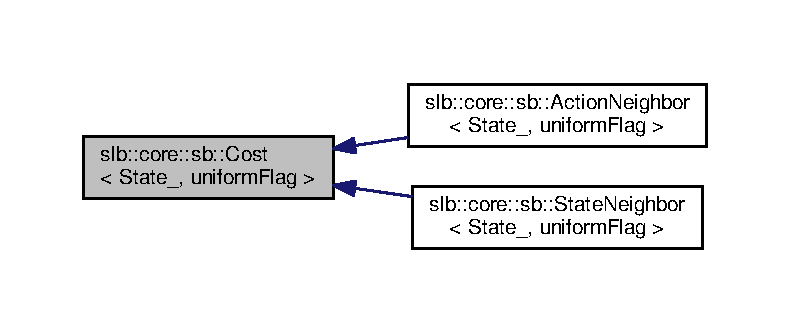
\includegraphics[width=350pt]{structslb_1_1core_1_1sb_1_1Cost__inherit__graph}
\end{center}
\end{figure}
\subsubsection*{Public Types}
\begin{DoxyCompactItemize}
\item 
using \hyperlink{structslb_1_1core_1_1sb_1_1Cost_af5d4c57aa664e5ae63eb365e1cecaf92}{State} = State\+\_\+\hypertarget{structslb_1_1core_1_1sb_1_1Cost_af5d4c57aa664e5ae63eb365e1cecaf92}{}\label{structslb_1_1core_1_1sb_1_1Cost_af5d4c57aa664e5ae63eb365e1cecaf92}

\begin{DoxyCompactList}\small\item\em The state type, represents the domain. \end{DoxyCompactList}\item 
using \hyperlink{structslb_1_1core_1_1sb_1_1Cost_a383726dcecbf69f396aa3a6d34b60278}{Cost\+Type} = typename State\+::\+Cost\+Type\hypertarget{structslb_1_1core_1_1sb_1_1Cost_a383726dcecbf69f396aa3a6d34b60278}{}\label{structslb_1_1core_1_1sb_1_1Cost_a383726dcecbf69f396aa3a6d34b60278}

\begin{DoxyCompactList}\small\item\em Action cost type. \end{DoxyCompactList}\end{DoxyCompactItemize}
\subsubsection*{Public Member Functions}
\begin{DoxyCompactItemize}
\item 
\hyperlink{structslb_1_1core_1_1sb_1_1Cost_afee978039270c56faa54b1f9380058ee}{Cost} (\hyperlink{structslb_1_1core_1_1sb_1_1Cost_a383726dcecbf69f396aa3a6d34b60278}{Cost\+Type} c)
\begin{DoxyCompactList}\small\item\em Constructor. \end{DoxyCompactList}\item 
\hyperlink{structslb_1_1core_1_1sb_1_1Cost_a383726dcecbf69f396aa3a6d34b60278}{Cost\+Type} \hyperlink{structslb_1_1core_1_1sb_1_1Cost_a5733d9b60a0bffaa1b69b351618fc6ae}{cost} () const 
\begin{DoxyCompactList}\small\item\em Returns cost of the action that leads to the neighbor state. \end{DoxyCompactList}\end{DoxyCompactItemize}
\subsubsection*{Private Attributes}
\begin{DoxyCompactItemize}
\item 
\hyperlink{structslb_1_1core_1_1sb_1_1Cost_a383726dcecbf69f396aa3a6d34b60278}{Cost\+Type} \hyperlink{structslb_1_1core_1_1sb_1_1Cost_ab337a97a0c3954e33229de4f0e1c6b29}{cost\+\_\+}\hypertarget{structslb_1_1core_1_1sb_1_1Cost_ab337a97a0c3954e33229de4f0e1c6b29}{}\label{structslb_1_1core_1_1sb_1_1Cost_ab337a97a0c3954e33229de4f0e1c6b29}

\begin{DoxyCompactList}\small\item\em Action cost. \end{DoxyCompactList}\end{DoxyCompactItemize}


\subsubsection{Detailed Description}
\subsubsection*{template$<$typename State\+\_\+, bool uniform\+Flag = true$>$\\*
struct slb\+::core\+::sb\+::\+Cost$<$ State\+\_\+, uniform\+Flag $>$}

The type for storing the cost of a neighbor. 


\begin{DoxyTemplParams}{Template Parameters}
{\em State} & The state type, represents the domain. \\
\hline
{\em uniform\+Flag} & Determines whether the domain is a uniform cost one or not. \\
\hline
\end{DoxyTemplParams}


Definition at line 16 of file neighbor.\+h.



\subsubsection{Constructor \& Destructor Documentation}
\index{slb\+::core\+::sb\+::\+Cost@{slb\+::core\+::sb\+::\+Cost}!Cost@{Cost}}
\index{Cost@{Cost}!slb\+::core\+::sb\+::\+Cost@{slb\+::core\+::sb\+::\+Cost}}
\paragraph[{\texorpdfstring{Cost(\+Cost\+Type c)}{Cost(CostType c)}}]{\setlength{\rightskip}{0pt plus 5cm}template$<$typename State\+\_\+ , bool uniform\+Flag = true$>$ {\bf slb\+::core\+::sb\+::\+Cost}$<$ State\+\_\+, uniform\+Flag $>$\+::{\bf Cost} (
\begin{DoxyParamCaption}
\item[{{\bf Cost\+Type}}]{c}
\end{DoxyParamCaption}
)\hspace{0.3cm}{\ttfamily [inline]}}\hypertarget{structslb_1_1core_1_1sb_1_1Cost_afee978039270c56faa54b1f9380058ee}{}\label{structslb_1_1core_1_1sb_1_1Cost_afee978039270c56faa54b1f9380058ee}


Constructor. 


\begin{DoxyParams}{Parameters}
{\em c} & The cost. \\
\hline
\end{DoxyParams}


Definition at line 22 of file neighbor.\+h.



\subsubsection{Member Function Documentation}
\index{slb\+::core\+::sb\+::\+Cost@{slb\+::core\+::sb\+::\+Cost}!cost@{cost}}
\index{cost@{cost}!slb\+::core\+::sb\+::\+Cost@{slb\+::core\+::sb\+::\+Cost}}
\paragraph[{\texorpdfstring{cost() const }{cost() const }}]{\setlength{\rightskip}{0pt plus 5cm}template$<$typename State\+\_\+ , bool uniform\+Flag = true$>$ {\bf Cost\+Type} {\bf slb\+::core\+::sb\+::\+Cost}$<$ State\+\_\+, uniform\+Flag $>$\+::cost (
\begin{DoxyParamCaption}
{}
\end{DoxyParamCaption}
) const\hspace{0.3cm}{\ttfamily [inline]}}\hypertarget{structslb_1_1core_1_1sb_1_1Cost_a5733d9b60a0bffaa1b69b351618fc6ae}{}\label{structslb_1_1core_1_1sb_1_1Cost_a5733d9b60a0bffaa1b69b351618fc6ae}


Returns cost of the action that leads to the neighbor state. 

\begin{DoxyReturn}{Returns}
\hyperlink{structslb_1_1core_1_1sb_1_1Cost}{Cost} of the action that leads to the neighbor state. 
\end{DoxyReturn}


Definition at line 26 of file neighbor.\+h.



The documentation for this struct was generated from the following file\+:\begin{DoxyCompactItemize}
\item 
core/search\+\_\+base/\hyperlink{neighbor_8h}{neighbor.\+h}\end{DoxyCompactItemize}

\hypertarget{structslb_1_1core_1_1sb_1_1Cost_3_01State___00_01true_01_4}{}\subsection{slb\+:\+:core\+:\+:sb\+:\+:Cost$<$ State\+\_\+, true $>$ Struct Template Reference}
\label{structslb_1_1core_1_1sb_1_1Cost_3_01State___00_01true_01_4}\index{slb\+::core\+::sb\+::\+Cost$<$ State\+\_\+, true $>$@{slb\+::core\+::sb\+::\+Cost$<$ State\+\_\+, true $>$}}


Specialization of the type for storing the cost of a neighbor for uniform domains.  




{\ttfamily \#include $<$neighbor.\+h$>$}

\subsubsection*{Public Types}
\begin{DoxyCompactItemize}
\item 
using \hyperlink{structslb_1_1core_1_1sb_1_1Cost_3_01State___00_01true_01_4_a205e1712d7e0e37db52599e38ce9fd32}{State} = State\+\_\+\hypertarget{structslb_1_1core_1_1sb_1_1Cost_3_01State___00_01true_01_4_a205e1712d7e0e37db52599e38ce9fd32}{}\label{structslb_1_1core_1_1sb_1_1Cost_3_01State___00_01true_01_4_a205e1712d7e0e37db52599e38ce9fd32}

\begin{DoxyCompactList}\small\item\em The state type, represents the domain. \end{DoxyCompactList}\item 
using \hyperlink{structslb_1_1core_1_1sb_1_1Cost_3_01State___00_01true_01_4_a13c4b693ea73bc79237bc51ec08f125c}{Cost\+Type} = typename State\+::\+Cost\+Type\hypertarget{structslb_1_1core_1_1sb_1_1Cost_3_01State___00_01true_01_4_a13c4b693ea73bc79237bc51ec08f125c}{}\label{structslb_1_1core_1_1sb_1_1Cost_3_01State___00_01true_01_4_a13c4b693ea73bc79237bc51ec08f125c}

\begin{DoxyCompactList}\small\item\em Action cost type. \end{DoxyCompactList}\end{DoxyCompactItemize}
\subsubsection*{Public Member Functions}
\begin{DoxyCompactItemize}
\item 
\hyperlink{structslb_1_1core_1_1sb_1_1Cost_3_01State___00_01true_01_4_a1bbfc5102b06386aaed54c23fcf65e50}{Cost} (\hyperlink{structslb_1_1core_1_1sb_1_1Cost_3_01State___00_01true_01_4_a13c4b693ea73bc79237bc51ec08f125c}{Cost\+Type})\hypertarget{structslb_1_1core_1_1sb_1_1Cost_3_01State___00_01true_01_4_a1bbfc5102b06386aaed54c23fcf65e50}{}\label{structslb_1_1core_1_1sb_1_1Cost_3_01State___00_01true_01_4_a1bbfc5102b06386aaed54c23fcf65e50}

\begin{DoxyCompactList}\small\item\em Constructor. \end{DoxyCompactList}\item 
constexpr \hyperlink{structslb_1_1core_1_1sb_1_1Cost_3_01State___00_01true_01_4_a13c4b693ea73bc79237bc51ec08f125c}{Cost\+Type} \hyperlink{structslb_1_1core_1_1sb_1_1Cost_3_01State___00_01true_01_4_a747e3d089f0b93d3d74d86d7212715f8}{cost} () const 
\begin{DoxyCompactList}\small\item\em Returns cost of the action that leads to the neighbor state. \end{DoxyCompactList}\end{DoxyCompactItemize}


\subsubsection{Detailed Description}
\subsubsection*{template$<$typename State\+\_\+$>$\\*
struct slb\+::core\+::sb\+::\+Cost$<$ State\+\_\+, true $>$}

Specialization of the type for storing the cost of a neighbor for uniform domains. 


\begin{DoxyTemplParams}{Template Parameters}
{\em State} & The state type, represents the domain. \\
\hline
{\em uniform\+Flag} & Determines whether the domain is a uniform cost one or not. \\
\hline
\end{DoxyTemplParams}


Definition at line 36 of file neighbor.\+h.



\subsubsection{Member Function Documentation}
\index{slb\+::core\+::sb\+::\+Cost$<$ State\+\_\+, true $>$@{slb\+::core\+::sb\+::\+Cost$<$ State\+\_\+, true $>$}!cost@{cost}}
\index{cost@{cost}!slb\+::core\+::sb\+::\+Cost$<$ State\+\_\+, true $>$@{slb\+::core\+::sb\+::\+Cost$<$ State\+\_\+, true $>$}}
\paragraph[{\texorpdfstring{cost() const }{cost() const }}]{\setlength{\rightskip}{0pt plus 5cm}template$<$typename State\+\_\+ $>$ constexpr {\bf Cost\+Type} {\bf slb\+::core\+::sb\+::\+Cost}$<$ State\+\_\+, true $>$\+::cost (
\begin{DoxyParamCaption}
{}
\end{DoxyParamCaption}
) const\hspace{0.3cm}{\ttfamily [inline]}}\hypertarget{structslb_1_1core_1_1sb_1_1Cost_3_01State___00_01true_01_4_a747e3d089f0b93d3d74d86d7212715f8}{}\label{structslb_1_1core_1_1sb_1_1Cost_3_01State___00_01true_01_4_a747e3d089f0b93d3d74d86d7212715f8}


Returns cost of the action that leads to the neighbor state. 

\begin{DoxyReturn}{Returns}
\hyperlink{structslb_1_1core_1_1sb_1_1Cost}{Cost} of the action that leads to the neighbor state. 
\end{DoxyReturn}


Definition at line 45 of file neighbor.\+h.



The documentation for this struct was generated from the following file\+:\begin{DoxyCompactItemize}
\item 
core/search\+\_\+base/\hyperlink{neighbor_8h}{neighbor.\+h}\end{DoxyCompactItemize}

\hypertarget{structslb_1_1ext_1_1instanceMeasure_1_1CostGoal0Goal1}{}\subsection{slb\+:\+:ext\+:\+:instance\+Measure\+:\+:Cost\+Goal0\+Goal1 Struct Reference}
\label{structslb_1_1ext_1_1instanceMeasure_1_1CostGoal0Goal1}\index{slb\+::ext\+::instance\+Measure\+::\+Cost\+Goal0\+Goal1@{slb\+::ext\+::instance\+Measure\+::\+Cost\+Goal0\+Goal1}}


One additional instance measure -- the distance between the first two goals.  




{\ttfamily \#include $<$instance\+\_\+measures.\+h$>$}



Inheritance diagram for slb\+:\+:ext\+:\+:instance\+Measure\+:\+:Cost\+Goal0\+Goal1\+:\nopagebreak
\begin{figure}[H]
\begin{center}
\leavevmode
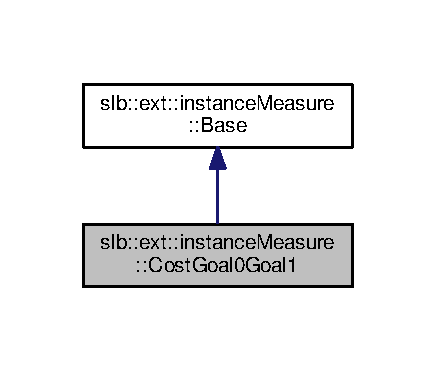
\includegraphics[width=209pt]{structslb_1_1ext_1_1instanceMeasure_1_1CostGoal0Goal1__inherit__graph}
\end{center}
\end{figure}


Collaboration diagram for slb\+:\+:ext\+:\+:instance\+Measure\+:\+:Cost\+Goal0\+Goal1\+:\nopagebreak
\begin{figure}[H]
\begin{center}
\leavevmode
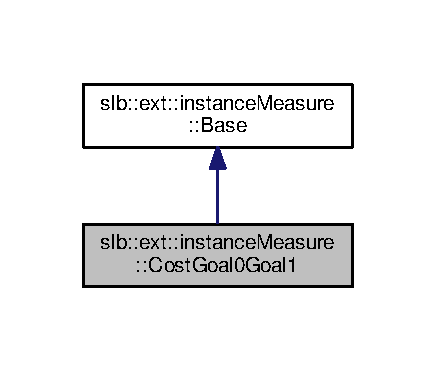
\includegraphics[width=209pt]{structslb_1_1ext_1_1instanceMeasure_1_1CostGoal0Goal1__coll__graph}
\end{center}
\end{figure}
\subsubsection*{Public Member Functions}
\begin{DoxyCompactItemize}
\item 
{\footnotesize template$<$class Instance $>$ }\\\hyperlink{structslb_1_1core_1_1sb_1_1MeasureSet}{Measure\+Set} \hyperlink{structslb_1_1ext_1_1instanceMeasure_1_1CostGoal0Goal1_a5b8f8b223cf0405a93685af269986dbb}{operator()} (const \hyperlink{structslb_1_1core_1_1sb_1_1Instance}{Instance} \&instance)
\begin{DoxyCompactList}\small\item\em Call operator to compute the measures. \end{DoxyCompactList}\end{DoxyCompactItemize}


\subsubsection{Detailed Description}
One additional instance measure -- the distance between the first two goals. 

Definition at line 38 of file instance\+\_\+measures.\+h.



\subsubsection{Member Function Documentation}
\index{slb\+::ext\+::instance\+Measure\+::\+Cost\+Goal0\+Goal1@{slb\+::ext\+::instance\+Measure\+::\+Cost\+Goal0\+Goal1}!operator()@{operator()}}
\index{operator()@{operator()}!slb\+::ext\+::instance\+Measure\+::\+Cost\+Goal0\+Goal1@{slb\+::ext\+::instance\+Measure\+::\+Cost\+Goal0\+Goal1}}
\paragraph[{\texorpdfstring{operator()(const Instance \&instance)}{operator()(const Instance &instance)}}]{\setlength{\rightskip}{0pt plus 5cm}template$<$class Instance $>$ {\bf Measure\+Set} slb\+::ext\+::instance\+Measure\+::\+Cost\+Goal0\+Goal1\+::operator() (
\begin{DoxyParamCaption}
\item[{const {\bf Instance} \&}]{instance}
\end{DoxyParamCaption}
)\hspace{0.3cm}{\ttfamily [inline]}}\hypertarget{structslb_1_1ext_1_1instanceMeasure_1_1CostGoal0Goal1_a5b8f8b223cf0405a93685af269986dbb}{}\label{structslb_1_1ext_1_1instanceMeasure_1_1CostGoal0Goal1_a5b8f8b223cf0405a93685af269986dbb}


Call operator to compute the measures. 


\begin{DoxyTemplParams}{Template Parameters}
{\em Instance} & The instance type. \\
\hline
\end{DoxyTemplParams}

\begin{DoxyParams}{Parameters}
{\em instance} & The instance. \\
\hline
\end{DoxyParams}
\begin{DoxyReturn}{Returns}
The measures of {\ttfamily instance}. 
\end{DoxyReturn}


Definition at line 43 of file instance\+\_\+measures.\+h.



The documentation for this struct was generated from the following file\+:\begin{DoxyCompactItemize}
\item 
extensions/instance\+\_\+measures/\hyperlink{instance__measures_8h}{instance\+\_\+measures.\+h}\end{DoxyCompactItemize}

\hypertarget{structslb_1_1core_1_1ui_1_1CurrentStyles}{}\subsection{slb\+:\+:core\+:\+:ui\+:\+:Current\+Styles$<$ State $>$ Struct Template Reference}
\label{structslb_1_1core_1_1ui_1_1CurrentStyles}\index{slb\+::core\+::ui\+::\+Current\+Styles$<$ State $>$@{slb\+::core\+::ui\+::\+Current\+Styles$<$ State $>$}}


A class for storing the current styles of vertices and edges in the visual representation.  




{\ttfamily \#include $<$current\+\_\+styles.\+h$>$}



Collaboration diagram for slb\+:\+:core\+:\+:ui\+:\+:Current\+Styles$<$ State $>$\+:\nopagebreak
\begin{figure}[H]
\begin{center}
\leavevmode
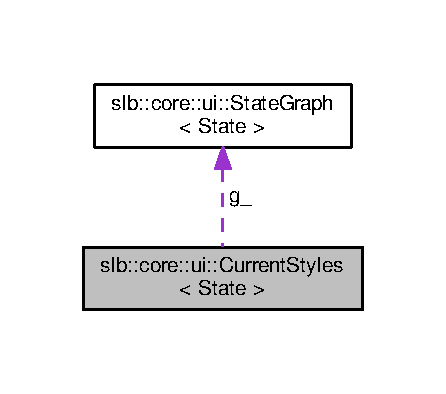
\includegraphics[width=214pt]{structslb_1_1core_1_1ui_1_1CurrentStyles__coll__graph}
\end{center}
\end{figure}
\subsubsection*{Public Types}
\begin{DoxyCompactItemize}
\item 
using \hyperlink{structslb_1_1core_1_1ui_1_1CurrentStyles_a2e3a5865892f484dcf9c94ac70bc19c2}{State\+Shared\+Ptr} = \hyperlink{classslb_1_1core_1_1util_1_1deref__shared__ptr}{deref\+\_\+shared\+\_\+ptr}$<$ const State $>$\hypertarget{structslb_1_1core_1_1ui_1_1CurrentStyles_a2e3a5865892f484dcf9c94ac70bc19c2}{}\label{structslb_1_1core_1_1ui_1_1CurrentStyles_a2e3a5865892f484dcf9c94ac70bc19c2}

\begin{DoxyCompactList}\small\item\em Smart pointer to state. \end{DoxyCompactList}\item 
using \hyperlink{structslb_1_1core_1_1ui_1_1CurrentStyles_ac27c6fba620b638233a5c620f68c89bc}{Graph} = \hyperlink{structslb_1_1core_1_1ui_1_1StateGraph}{State\+Graph}$<$ State $>$\hypertarget{structslb_1_1core_1_1ui_1_1CurrentStyles_ac27c6fba620b638233a5c620f68c89bc}{}\label{structslb_1_1core_1_1ui_1_1CurrentStyles_ac27c6fba620b638233a5c620f68c89bc}

\begin{DoxyCompactList}\small\item\em The graph type. \end{DoxyCompactList}\item 
using \hyperlink{structslb_1_1core_1_1ui_1_1CurrentStyles_a5da5348d833acc6d19d20556f00765b9}{Vertex\+Descriptor} = typename \hyperlink{structslb_1_1core_1_1ui_1_1StateGraph_ab2d88fce7d30dc6346910900212a7e6d}{Graph\+::\+Vertex\+Descriptor}\hypertarget{structslb_1_1core_1_1ui_1_1CurrentStyles_a5da5348d833acc6d19d20556f00765b9}{}\label{structslb_1_1core_1_1ui_1_1CurrentStyles_a5da5348d833acc6d19d20556f00765b9}

\begin{DoxyCompactList}\small\item\em Vertex identifier. \end{DoxyCompactList}\item 
using \hyperlink{structslb_1_1core_1_1ui_1_1CurrentStyles_aa63947c6380258a6f5147c75d3168e2a}{Edge\+Descriptor} = typename \hyperlink{structslb_1_1core_1_1ui_1_1StateGraph_a7e894f002383b1687652a91549c3656d}{Graph\+::\+Edge\+Descriptor}\hypertarget{structslb_1_1core_1_1ui_1_1CurrentStyles_aa63947c6380258a6f5147c75d3168e2a}{}\label{structslb_1_1core_1_1ui_1_1CurrentStyles_aa63947c6380258a6f5147c75d3168e2a}

\begin{DoxyCompactList}\small\item\em Edge identifier. \end{DoxyCompactList}\end{DoxyCompactItemize}
\subsubsection*{Public Member Functions}
\begin{DoxyCompactItemize}
\item 
\hyperlink{structslb_1_1core_1_1ui_1_1CurrentStyles_ab74d558873a0fab90d5ceace8aa2079d}{Current\+Styles} (const \hyperlink{structslb_1_1core_1_1ui_1_1CurrentStyles_ac27c6fba620b638233a5c620f68c89bc}{Graph} \&g)\hypertarget{structslb_1_1core_1_1ui_1_1CurrentStyles_ab74d558873a0fab90d5ceace8aa2079d}{}\label{structslb_1_1core_1_1ui_1_1CurrentStyles_ab74d558873a0fab90d5ceace8aa2079d}

\begin{DoxyCompactList}\small\item\em Initializes graph. \end{DoxyCompactList}\item 
\hyperlink{structslb_1_1core_1_1ui_1_1VertexStyle}{Vertex\+Style} \hyperlink{structslb_1_1core_1_1ui_1_1CurrentStyles_a201c59d8806f1a6eace1df2dff8143c6}{get} (\hyperlink{structslb_1_1core_1_1ui_1_1CurrentStyles_a5da5348d833acc6d19d20556f00765b9}{Vertex\+Descriptor} vd) const 
\begin{DoxyCompactList}\small\item\em Returns the current style of the given vertex. \end{DoxyCompactList}\item 
\hyperlink{structslb_1_1core_1_1ui_1_1EdgeStyle}{Edge\+Style} \hyperlink{structslb_1_1core_1_1ui_1_1CurrentStyles_ac251d1fbd39198cb34642e7138727495}{get} (\hyperlink{structslb_1_1core_1_1ui_1_1CurrentStyles_aa63947c6380258a6f5147c75d3168e2a}{Edge\+Descriptor} ed) const 
\begin{DoxyCompactList}\small\item\em Returns the current style of the given edge. \end{DoxyCompactList}\item 
\hyperlink{structslb_1_1core_1_1ui_1_1VertexStyle}{Vertex\+Style} \hyperlink{structslb_1_1core_1_1ui_1_1CurrentStyles_ae2f28e0dcb6e8d38a6710a7b0f21e568}{get} (\hyperlink{structslb_1_1core_1_1ui_1_1CurrentStyles_a2e3a5865892f484dcf9c94ac70bc19c2}{State\+Shared\+Ptr} s) const 
\begin{DoxyCompactList}\small\item\em Returns the current style of the vertex representing a given state. \end{DoxyCompactList}\item 
\hyperlink{structslb_1_1core_1_1ui_1_1EdgeStyle}{Edge\+Style} \hyperlink{structslb_1_1core_1_1ui_1_1CurrentStyles_a7a75762ed7d0343867b5bf29c08b7b81}{get} (\hyperlink{structslb_1_1core_1_1ui_1_1CurrentStyles_a2e3a5865892f484dcf9c94ac70bc19c2}{State\+Shared\+Ptr} from, \hyperlink{structslb_1_1core_1_1ui_1_1CurrentStyles_a2e3a5865892f484dcf9c94ac70bc19c2}{State\+Shared\+Ptr} to) const 
\begin{DoxyCompactList}\small\item\em Returns the current style of the edge between the given state. \end{DoxyCompactList}\end{DoxyCompactItemize}
\subsubsection*{Protected Attributes}
\begin{DoxyCompactItemize}
\item 
const \hyperlink{structslb_1_1core_1_1ui_1_1CurrentStyles_ac27c6fba620b638233a5c620f68c89bc}{Graph} \& \hyperlink{structslb_1_1core_1_1ui_1_1CurrentStyles_a4f67551367b7b4dc17f93df96d51c864}{g\+\_\+}\hypertarget{structslb_1_1core_1_1ui_1_1CurrentStyles_a4f67551367b7b4dc17f93df96d51c864}{}\label{structslb_1_1core_1_1ui_1_1CurrentStyles_a4f67551367b7b4dc17f93df96d51c864}

\begin{DoxyCompactList}\small\item\em The graph. \end{DoxyCompactList}\item 
std\+::unordered\+\_\+map$<$ \hyperlink{structslb_1_1core_1_1ui_1_1CurrentStyles_a5da5348d833acc6d19d20556f00765b9}{Vertex\+Descriptor}, \hyperlink{structslb_1_1core_1_1ui_1_1VertexStyle}{Vertex\+Style} $>$ \hyperlink{structslb_1_1core_1_1ui_1_1CurrentStyles_ab6f530b659136f839b7f51dbe15a8b8c}{vertex\+Styles\+\_\+}\hypertarget{structslb_1_1core_1_1ui_1_1CurrentStyles_ab6f530b659136f839b7f51dbe15a8b8c}{}\label{structslb_1_1core_1_1ui_1_1CurrentStyles_ab6f530b659136f839b7f51dbe15a8b8c}

\begin{DoxyCompactList}\small\item\em Mapping from each vertex to its style. \end{DoxyCompactList}\item 
std\+::map$<$ \hyperlink{structslb_1_1core_1_1ui_1_1CurrentStyles_aa63947c6380258a6f5147c75d3168e2a}{Edge\+Descriptor}, \hyperlink{structslb_1_1core_1_1ui_1_1EdgeStyle}{Edge\+Style} $>$ \hyperlink{structslb_1_1core_1_1ui_1_1CurrentStyles_ac4c13a371872935d47ecebeded6620c9}{edge\+Styles\+\_\+}\hypertarget{structslb_1_1core_1_1ui_1_1CurrentStyles_ac4c13a371872935d47ecebeded6620c9}{}\label{structslb_1_1core_1_1ui_1_1CurrentStyles_ac4c13a371872935d47ecebeded6620c9}

\begin{DoxyCompactList}\small\item\em Mapping from each edge to its style. There is no hash function for \hyperlink{structslb_1_1core_1_1ui_1_1CurrentStyles_aa63947c6380258a6f5147c75d3168e2a}{Edge\+Descriptor}, hence a sorted map. \end{DoxyCompactList}\end{DoxyCompactItemize}


\subsubsection{Detailed Description}
\subsubsection*{template$<$class State$>$\\*
struct slb\+::core\+::ui\+::\+Current\+Styles$<$ State $>$}

A class for storing the current styles of vertices and edges in the visual representation. 


\begin{DoxyTemplParams}{Template Parameters}
{\em State} & The state type, represents the domain. \\
\hline
\end{DoxyTemplParams}


Definition at line 18 of file current\+\_\+styles.\+h.



\subsubsection{Member Function Documentation}
\index{slb\+::core\+::ui\+::\+Current\+Styles@{slb\+::core\+::ui\+::\+Current\+Styles}!get@{get}}
\index{get@{get}!slb\+::core\+::ui\+::\+Current\+Styles@{slb\+::core\+::ui\+::\+Current\+Styles}}
\paragraph[{\texorpdfstring{get(\+Vertex\+Descriptor vd) const }{get(VertexDescriptor vd) const }}]{\setlength{\rightskip}{0pt plus 5cm}template$<$class State$>$ {\bf Vertex\+Style} {\bf slb\+::core\+::ui\+::\+Current\+Styles}$<$ State $>$\+::get (
\begin{DoxyParamCaption}
\item[{{\bf Vertex\+Descriptor}}]{vd}
\end{DoxyParamCaption}
) const\hspace{0.3cm}{\ttfamily [inline]}}\hypertarget{structslb_1_1core_1_1ui_1_1CurrentStyles_a201c59d8806f1a6eace1df2dff8143c6}{}\label{structslb_1_1core_1_1ui_1_1CurrentStyles_a201c59d8806f1a6eace1df2dff8143c6}


Returns the current style of the given vertex. 


\begin{DoxyParams}{Parameters}
{\em vd} & Vertex identifier. \\
\hline
\end{DoxyParams}
\begin{DoxyReturn}{Returns}
The vertex style. 
\end{DoxyReturn}
\begin{DoxyPrecond}{Precondition}
The vertex must be present in the graph. 
\end{DoxyPrecond}


Definition at line 38 of file current\+\_\+styles.\+h.

\index{slb\+::core\+::ui\+::\+Current\+Styles@{slb\+::core\+::ui\+::\+Current\+Styles}!get@{get}}
\index{get@{get}!slb\+::core\+::ui\+::\+Current\+Styles@{slb\+::core\+::ui\+::\+Current\+Styles}}
\paragraph[{\texorpdfstring{get(\+Edge\+Descriptor ed) const }{get(EdgeDescriptor ed) const }}]{\setlength{\rightskip}{0pt plus 5cm}template$<$class State$>$ {\bf Edge\+Style} {\bf slb\+::core\+::ui\+::\+Current\+Styles}$<$ State $>$\+::get (
\begin{DoxyParamCaption}
\item[{{\bf Edge\+Descriptor}}]{ed}
\end{DoxyParamCaption}
) const\hspace{0.3cm}{\ttfamily [inline]}}\hypertarget{structslb_1_1core_1_1ui_1_1CurrentStyles_ac251d1fbd39198cb34642e7138727495}{}\label{structslb_1_1core_1_1ui_1_1CurrentStyles_ac251d1fbd39198cb34642e7138727495}


Returns the current style of the given edge. 


\begin{DoxyParams}{Parameters}
{\em ed} & Edge identifier. \\
\hline
\end{DoxyParams}
\begin{DoxyReturn}{Returns}
The edge style. 
\end{DoxyReturn}
\begin{DoxyPrecond}{Precondition}
The edge must be present in the graph. 
\end{DoxyPrecond}


Definition at line 52 of file current\+\_\+styles.\+h.

\index{slb\+::core\+::ui\+::\+Current\+Styles@{slb\+::core\+::ui\+::\+Current\+Styles}!get@{get}}
\index{get@{get}!slb\+::core\+::ui\+::\+Current\+Styles@{slb\+::core\+::ui\+::\+Current\+Styles}}
\paragraph[{\texorpdfstring{get(\+State\+Shared\+Ptr s) const }{get(StateSharedPtr s) const }}]{\setlength{\rightskip}{0pt plus 5cm}template$<$class State$>$ {\bf Vertex\+Style} {\bf slb\+::core\+::ui\+::\+Current\+Styles}$<$ State $>$\+::get (
\begin{DoxyParamCaption}
\item[{{\bf State\+Shared\+Ptr}}]{s}
\end{DoxyParamCaption}
) const\hspace{0.3cm}{\ttfamily [inline]}}\hypertarget{structslb_1_1core_1_1ui_1_1CurrentStyles_ae2f28e0dcb6e8d38a6710a7b0f21e568}{}\label{structslb_1_1core_1_1ui_1_1CurrentStyles_ae2f28e0dcb6e8d38a6710a7b0f21e568}


Returns the current style of the vertex representing a given state. 


\begin{DoxyParams}{Parameters}
{\em s} & Shared pointer to state. \\
\hline
\end{DoxyParams}
\begin{DoxyReturn}{Returns}
The vertex style. 
\end{DoxyReturn}
\begin{DoxyPrecond}{Precondition}
The vertex corresponding to {\ttfamily s} must be present in the graph. 
\end{DoxyPrecond}


Definition at line 60 of file current\+\_\+styles.\+h.

\index{slb\+::core\+::ui\+::\+Current\+Styles@{slb\+::core\+::ui\+::\+Current\+Styles}!get@{get}}
\index{get@{get}!slb\+::core\+::ui\+::\+Current\+Styles@{slb\+::core\+::ui\+::\+Current\+Styles}}
\paragraph[{\texorpdfstring{get(\+State\+Shared\+Ptr from, State\+Shared\+Ptr to) const }{get(StateSharedPtr from, StateSharedPtr to) const }}]{\setlength{\rightskip}{0pt plus 5cm}template$<$class State$>$ {\bf Edge\+Style} {\bf slb\+::core\+::ui\+::\+Current\+Styles}$<$ State $>$\+::get (
\begin{DoxyParamCaption}
\item[{{\bf State\+Shared\+Ptr}}]{from, }
\item[{{\bf State\+Shared\+Ptr}}]{to}
\end{DoxyParamCaption}
) const\hspace{0.3cm}{\ttfamily [inline]}}\hypertarget{structslb_1_1core_1_1ui_1_1CurrentStyles_a7a75762ed7d0343867b5bf29c08b7b81}{}\label{structslb_1_1core_1_1ui_1_1CurrentStyles_a7a75762ed7d0343867b5bf29c08b7b81}


Returns the current style of the edge between the given state. 


\begin{DoxyParams}{Parameters}
{\em from} & Shared pointer to the source state. \\
\hline
{\em to} & Shared pointer to the target state. \\
\hline
\end{DoxyParams}
\begin{DoxyReturn}{Returns}
The edge style. 
\end{DoxyReturn}
\begin{DoxyPrecond}{Precondition}
The edge must be present in the graph. 
\end{DoxyPrecond}


Definition at line 69 of file current\+\_\+styles.\+h.



The documentation for this struct was generated from the following file\+:\begin{DoxyCompactItemize}
\item 
core/user\+\_\+interface/\hyperlink{current__styles_8h}{current\+\_\+styles.\+h}\end{DoxyCompactItemize}

\hypertarget{structslb_1_1ext_1_1policy_1_1openList_1_1DefaultOLKeyType}{}\subsection{slb\+:\+:ext\+:\+:policy\+:\+:open\+List\+:\+:Default\+O\+L\+Key\+Type$<$ Node $>$ Struct Template Reference}
\label{structslb_1_1ext_1_1policy_1_1openList_1_1DefaultOLKeyType}\index{slb\+::ext\+::policy\+::open\+List\+::\+Default\+O\+L\+Key\+Type$<$ Node $>$@{slb\+::ext\+::policy\+::open\+List\+::\+Default\+O\+L\+Key\+Type$<$ Node $>$}}


Nodes are ordered in the open list based on g and f. The particular ordering rules are defined by the other policies.  




{\ttfamily \#include $<$open\+\_\+list.\+h$>$}

\subsubsection*{Public Types}
\begin{DoxyCompactItemize}
\item 
using \hyperlink{structslb_1_1ext_1_1policy_1_1openList_1_1DefaultOLKeyType_afdae8b0b1b4427bc68c40ecd960cf1ab}{Cost\+Type} = typename Node\+::\+Cost\+Type\hypertarget{structslb_1_1ext_1_1policy_1_1openList_1_1DefaultOLKeyType_afdae8b0b1b4427bc68c40ecd960cf1ab}{}\label{structslb_1_1ext_1_1policy_1_1openList_1_1DefaultOLKeyType_afdae8b0b1b4427bc68c40ecd960cf1ab}

\begin{DoxyCompactList}\small\item\em Type for action cost. \end{DoxyCompactList}\end{DoxyCompactItemize}
\subsubsection*{Public Member Functions}
\begin{DoxyCompactItemize}
\item 
\hyperlink{structslb_1_1ext_1_1policy_1_1openList_1_1DefaultOLKeyType_ad5dd2f1bd5ba1c35ed0f197b58d6823a}{Default\+O\+L\+Key\+Type} (const Node $\ast$n)
\begin{DoxyCompactList}\small\item\em Initializes the key based on the node. \end{DoxyCompactList}\end{DoxyCompactItemize}
\subsubsection*{Public Attributes}
\begin{DoxyCompactItemize}
\item 
\hyperlink{structslb_1_1ext_1_1policy_1_1openList_1_1DefaultOLKeyType_afdae8b0b1b4427bc68c40ecd960cf1ab}{Cost\+Type} \hyperlink{structslb_1_1ext_1_1policy_1_1openList_1_1DefaultOLKeyType_a89a082636c1559e23c33651906b9a73b}{g}\hypertarget{structslb_1_1ext_1_1policy_1_1openList_1_1DefaultOLKeyType_a89a082636c1559e23c33651906b9a73b}{}\label{structslb_1_1ext_1_1policy_1_1openList_1_1DefaultOLKeyType_a89a082636c1559e23c33651906b9a73b}

\begin{DoxyCompactList}\small\item\em g-\/cost of the node. \end{DoxyCompactList}\item 
\hyperlink{structslb_1_1ext_1_1policy_1_1openList_1_1DefaultOLKeyType_afdae8b0b1b4427bc68c40ecd960cf1ab}{Cost\+Type} \hyperlink{structslb_1_1ext_1_1policy_1_1openList_1_1DefaultOLKeyType_a5ed8cd631d87833d34fccc76880df2e3}{f}\hypertarget{structslb_1_1ext_1_1policy_1_1openList_1_1DefaultOLKeyType_a5ed8cd631d87833d34fccc76880df2e3}{}\label{structslb_1_1ext_1_1policy_1_1openList_1_1DefaultOLKeyType_a5ed8cd631d87833d34fccc76880df2e3}

\begin{DoxyCompactList}\small\item\em f-\/cost of the node. \end{DoxyCompactList}\end{DoxyCompactItemize}


\subsubsection{Detailed Description}
\subsubsection*{template$<$class Node$>$\\*
struct slb\+::ext\+::policy\+::open\+List\+::\+Default\+O\+L\+Key\+Type$<$ Node $>$}

Nodes are ordered in the open list based on g and f. The particular ordering rules are defined by the other policies. 


\begin{DoxyTemplParams}{Template Parameters}
{\em Node} & The node type. \\
\hline
\end{DoxyTemplParams}


Definition at line 34 of file open\+\_\+list.\+h.



\subsubsection{Constructor \& Destructor Documentation}
\index{slb\+::ext\+::policy\+::open\+List\+::\+Default\+O\+L\+Key\+Type@{slb\+::ext\+::policy\+::open\+List\+::\+Default\+O\+L\+Key\+Type}!Default\+O\+L\+Key\+Type@{Default\+O\+L\+Key\+Type}}
\index{Default\+O\+L\+Key\+Type@{Default\+O\+L\+Key\+Type}!slb\+::ext\+::policy\+::open\+List\+::\+Default\+O\+L\+Key\+Type@{slb\+::ext\+::policy\+::open\+List\+::\+Default\+O\+L\+Key\+Type}}
\paragraph[{\texorpdfstring{Default\+O\+L\+Key\+Type(const Node $\ast$n)}{DefaultOLKeyType(const Node *n)}}]{\setlength{\rightskip}{0pt plus 5cm}template$<$class Node$>$ {\bf slb\+::ext\+::policy\+::open\+List\+::\+Default\+O\+L\+Key\+Type}$<$ Node $>$\+::{\bf Default\+O\+L\+Key\+Type} (
\begin{DoxyParamCaption}
\item[{const Node $\ast$}]{n}
\end{DoxyParamCaption}
)\hspace{0.3cm}{\ttfamily [inline]}}\hypertarget{structslb_1_1ext_1_1policy_1_1openList_1_1DefaultOLKeyType_ad5dd2f1bd5ba1c35ed0f197b58d6823a}{}\label{structslb_1_1ext_1_1policy_1_1openList_1_1DefaultOLKeyType_ad5dd2f1bd5ba1c35ed0f197b58d6823a}


Initializes the key based on the node. 


\begin{DoxyParams}{Parameters}
{\em n} & The node. \\
\hline
\end{DoxyParams}


Definition at line 41 of file open\+\_\+list.\+h.



The documentation for this struct was generated from the following file\+:\begin{DoxyCompactItemize}
\item 
extensions/shared\+\_\+policies/\hyperlink{open__list_8h}{open\+\_\+list.\+h}\end{DoxyCompactItemize}

\hypertarget{structslb_1_1ext_1_1event_1_1DeniedExpansion}{}\subsection{slb\+:\+:ext\+:\+:event\+:\+:Denied\+Expansion$<$ Node $>$ Struct Template Reference}
\label{structslb_1_1ext_1_1event_1_1DeniedExpansion}\index{slb\+::ext\+::event\+::\+Denied\+Expansion$<$ Node $>$@{slb\+::ext\+::event\+::\+Denied\+Expansion$<$ Node $>$}}


Event that visualizes a node\textquotesingle{}s expansion being denied following suspension (see \hyperlink{structslb_1_1ext_1_1event_1_1SuspendedExpansion}{Suspended\+Expansion}).  




{\ttfamily \#include $<$events.\+h$>$}



Inheritance diagram for slb\+:\+:ext\+:\+:event\+:\+:Denied\+Expansion$<$ Node $>$\+:\nopagebreak
\begin{figure}[H]
\begin{center}
\leavevmode
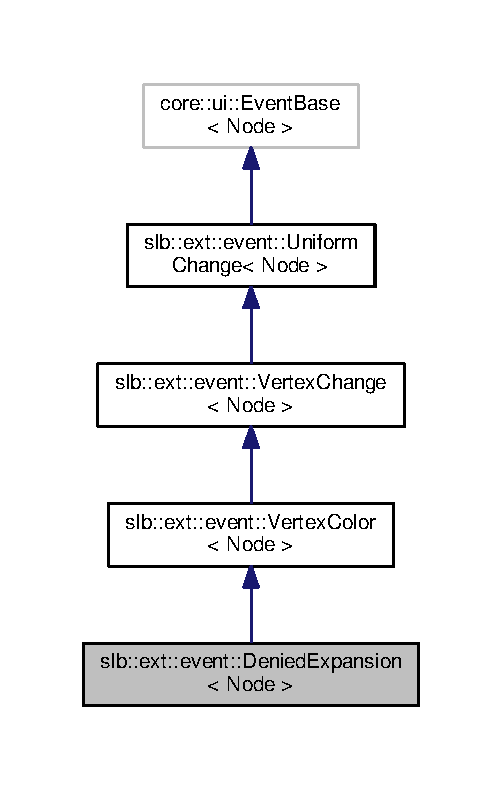
\includegraphics[width=241pt]{structslb_1_1ext_1_1event_1_1DeniedExpansion__inherit__graph}
\end{center}
\end{figure}


Collaboration diagram for slb\+:\+:ext\+:\+:event\+:\+:Denied\+Expansion$<$ Node $>$\+:\nopagebreak
\begin{figure}[H]
\begin{center}
\leavevmode
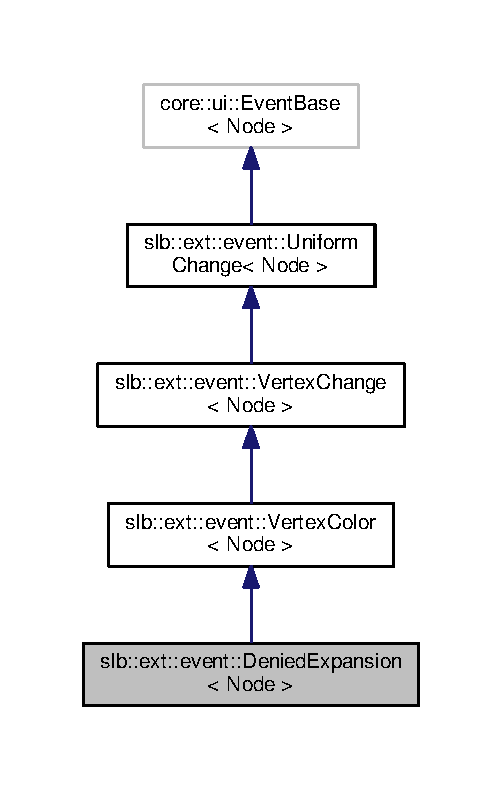
\includegraphics[width=241pt]{structslb_1_1ext_1_1event_1_1DeniedExpansion__coll__graph}
\end{center}
\end{figure}
\subsubsection*{Private Member Functions}
\begin{DoxyCompactItemize}
\item 
virtual Color \hyperlink{structslb_1_1ext_1_1event_1_1DeniedExpansion_a6f2aa3f5f67e00c2c30aebd472872eda}{color} () const override
\begin{DoxyCompactList}\small\item\em Returns the new color of the vertex corresponding to the state associated with the event. \end{DoxyCompactList}\item 
std\+::string \hyperlink{structslb_1_1ext_1_1event_1_1DeniedExpansion_a159ac4c3963cd068b40d90ed30b75b3d}{event\+Str} () const override
\begin{DoxyCompactList}\small\item\em Returns the string describing the event. This string is displayed in the log window. \end{DoxyCompactList}\end{DoxyCompactItemize}
\subsubsection*{Additional Inherited Members}


\subsubsection{Detailed Description}
\subsubsection*{template$<$class Node = S\+L\+B\+\_\+\+N\+O\+DE$>$\\*
struct slb\+::ext\+::event\+::\+Denied\+Expansion$<$ Node $>$}

Event that visualizes a node\textquotesingle{}s expansion being denied following suspension (see \hyperlink{structslb_1_1ext_1_1event_1_1SuspendedExpansion}{Suspended\+Expansion}). 


\begin{DoxyTemplParams}{Template Parameters}
{\em Node} & The search node type. \\
\hline
\end{DoxyTemplParams}


Definition at line 220 of file events.\+h.



\subsubsection{Member Function Documentation}
\index{slb\+::ext\+::event\+::\+Denied\+Expansion@{slb\+::ext\+::event\+::\+Denied\+Expansion}!color@{color}}
\index{color@{color}!slb\+::ext\+::event\+::\+Denied\+Expansion@{slb\+::ext\+::event\+::\+Denied\+Expansion}}
\paragraph[{\texorpdfstring{color() const override}{color() const override}}]{\setlength{\rightskip}{0pt plus 5cm}template$<$class Node  = S\+L\+B\+\_\+\+N\+O\+DE$>$ virtual Color {\bf slb\+::ext\+::event\+::\+Denied\+Expansion}$<$ Node $>$\+::color (
\begin{DoxyParamCaption}
{}
\end{DoxyParamCaption}
) const\hspace{0.3cm}{\ttfamily [inline]}, {\ttfamily [override]}, {\ttfamily [private]}, {\ttfamily [virtual]}}\hypertarget{structslb_1_1ext_1_1event_1_1DeniedExpansion_a6f2aa3f5f67e00c2c30aebd472872eda}{}\label{structslb_1_1ext_1_1event_1_1DeniedExpansion_a6f2aa3f5f67e00c2c30aebd472872eda}


Returns the new color of the vertex corresponding to the state associated with the event. 

\begin{DoxyReturn}{Returns}
The new color of the vertex corresponding to the state associated with the event. 
\end{DoxyReturn}


Implements \hyperlink{structslb_1_1ext_1_1event_1_1VertexColor_a651aab95a9f39de56a70273c9d40a76f}{slb\+::ext\+::event\+::\+Vertex\+Color$<$ Node $>$}.



Definition at line 229 of file events.\+h.

\index{slb\+::ext\+::event\+::\+Denied\+Expansion@{slb\+::ext\+::event\+::\+Denied\+Expansion}!event\+Str@{event\+Str}}
\index{event\+Str@{event\+Str}!slb\+::ext\+::event\+::\+Denied\+Expansion@{slb\+::ext\+::event\+::\+Denied\+Expansion}}
\paragraph[{\texorpdfstring{event\+Str() const override}{eventStr() const override}}]{\setlength{\rightskip}{0pt plus 5cm}template$<$class Node  = S\+L\+B\+\_\+\+N\+O\+DE$>$ std\+::string {\bf slb\+::ext\+::event\+::\+Denied\+Expansion}$<$ Node $>$\+::event\+Str (
\begin{DoxyParamCaption}
{}
\end{DoxyParamCaption}
) const\hspace{0.3cm}{\ttfamily [inline]}, {\ttfamily [override]}, {\ttfamily [private]}}\hypertarget{structslb_1_1ext_1_1event_1_1DeniedExpansion_a159ac4c3963cd068b40d90ed30b75b3d}{}\label{structslb_1_1ext_1_1event_1_1DeniedExpansion_a159ac4c3963cd068b40d90ed30b75b3d}


Returns the string describing the event. This string is displayed in the log window. 

\begin{DoxyReturn}{Returns}
The string describing the event. 
\end{DoxyReturn}


Definition at line 234 of file events.\+h.



The documentation for this struct was generated from the following file\+:\begin{DoxyCompactItemize}
\item 
extensions/events/\hyperlink{events_8h}{events.\+h}\end{DoxyCompactItemize}

\hypertarget{classslb_1_1core_1_1util_1_1deref__shared__ptr}{}\subsection{slb\+:\+:core\+:\+:util\+:\+:deref\+\_\+shared\+\_\+ptr$<$ T $>$ Class Template Reference}
\label{classslb_1_1core_1_1util_1_1deref__shared__ptr}\index{slb\+::core\+::util\+::deref\+\_\+shared\+\_\+ptr$<$ T $>$@{slb\+::core\+::util\+::deref\+\_\+shared\+\_\+ptr$<$ T $>$}}


Shared pointer whose {\ttfamily operator==} compares the pointed to values.  




{\ttfamily \#include $<$memory.\+h$>$}



Inheritance diagram for slb\+:\+:core\+:\+:util\+:\+:deref\+\_\+shared\+\_\+ptr$<$ T $>$\+:\nopagebreak
\begin{figure}[H]
\begin{center}
\leavevmode
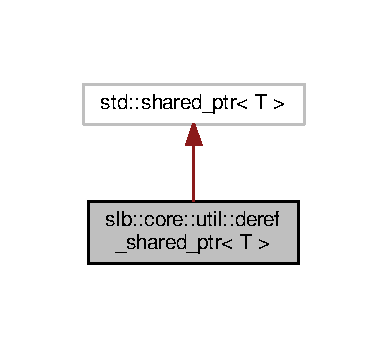
\includegraphics[width=186pt]{classslb_1_1core_1_1util_1_1deref__shared__ptr__inherit__graph}
\end{center}
\end{figure}


Collaboration diagram for slb\+:\+:core\+:\+:util\+:\+:deref\+\_\+shared\+\_\+ptr$<$ T $>$\+:\nopagebreak
\begin{figure}[H]
\begin{center}
\leavevmode
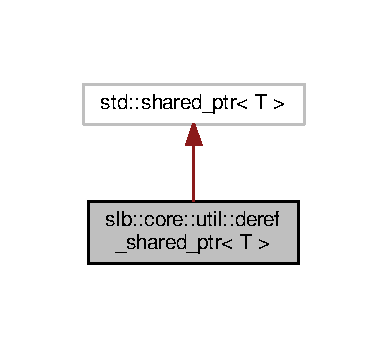
\includegraphics[width=186pt]{classslb_1_1core_1_1util_1_1deref__shared__ptr__coll__graph}
\end{center}
\end{figure}
\subsubsection*{Public Types}
\begin{DoxyCompactItemize}
\item 
using \hyperlink{classslb_1_1core_1_1util_1_1deref__shared__ptr_a288bb6317a3a5b58f0d1af011ec323f0}{Base} = std\+::shared\+\_\+ptr$<$ T $>$\hypertarget{classslb_1_1core_1_1util_1_1deref__shared__ptr_a288bb6317a3a5b58f0d1af011ec323f0}{}\label{classslb_1_1core_1_1util_1_1deref__shared__ptr_a288bb6317a3a5b58f0d1af011ec323f0}

\begin{DoxyCompactList}\small\item\em The standard shared pointer. \end{DoxyCompactList}\end{DoxyCompactItemize}
\subsubsection*{Public Member Functions}
\begin{DoxyCompactItemize}
\item 
constexpr \hyperlink{classslb_1_1core_1_1util_1_1deref__shared__ptr_a30431a65655696d226d519cb1538884d}{deref\+\_\+shared\+\_\+ptr} ()\hypertarget{classslb_1_1core_1_1util_1_1deref__shared__ptr_a30431a65655696d226d519cb1538884d}{}\label{classslb_1_1core_1_1util_1_1deref__shared__ptr_a30431a65655696d226d519cb1538884d}

\begin{DoxyCompactList}\small\item\em The default constructor. \end{DoxyCompactList}\item 
constexpr \hyperlink{classslb_1_1core_1_1util_1_1deref__shared__ptr_a739df6c589b420b635dfaa038d32bc96}{deref\+\_\+shared\+\_\+ptr} (std\+::nullptr\+\_\+t)\hypertarget{classslb_1_1core_1_1util_1_1deref__shared__ptr_a739df6c589b420b635dfaa038d32bc96}{}\label{classslb_1_1core_1_1util_1_1deref__shared__ptr_a739df6c589b420b635dfaa038d32bc96}

\begin{DoxyCompactList}\small\item\em The constructor based on {\ttfamily nullptr}. \end{DoxyCompactList}\item 
\hyperlink{classslb_1_1core_1_1util_1_1deref__shared__ptr_abeeb35b697324718b90d6e7b32561f6f}{deref\+\_\+shared\+\_\+ptr} (const \hyperlink{classslb_1_1core_1_1util_1_1deref__shared__ptr}{deref\+\_\+shared\+\_\+ptr} \&rhs)
\begin{DoxyCompactList}\small\item\em The copy constructor. \end{DoxyCompactList}\item 
{\footnotesize template$<$class Y $>$ }\\\hyperlink{classslb_1_1core_1_1util_1_1deref__shared__ptr_a61799e773215340c1f2f6a763d6ed308}{deref\+\_\+shared\+\_\+ptr} (Y $\ast$ptr)
\begin{DoxyCompactList}\small\item\em The constructor based on a pointer to a type that can be converted to {\ttfamily T}. \end{DoxyCompactList}\item 
{\footnotesize template$<$class Y , class Deleter $>$ }\\\hyperlink{classslb_1_1core_1_1util_1_1deref__shared__ptr_aaf5ef266fc89518c148b28e7260a869f}{deref\+\_\+shared\+\_\+ptr} (std\+::unique\+\_\+ptr$<$ Y, Deleter $>$ \&\&r)
\begin{DoxyCompactList}\small\item\em The moving constructor based on a unique pointer to a type that can be converted to {\ttfamily T}. \end{DoxyCompactList}\item 
\hyperlink{classslb_1_1core_1_1util_1_1deref__shared__ptr}{deref\+\_\+shared\+\_\+ptr} \& \hyperlink{classslb_1_1core_1_1util_1_1deref__shared__ptr_aec141838789d45a5d1d1bdf83a60d9cf}{operator=} (const \hyperlink{classslb_1_1core_1_1util_1_1deref__shared__ptr}{deref\+\_\+shared\+\_\+ptr} \&rhs)
\begin{DoxyCompactList}\small\item\em The assignment operator. \end{DoxyCompactList}\end{DoxyCompactItemize}
\subsubsection*{Private Member Functions}
\begin{DoxyCompactItemize}
\item 
\hyperlink{classslb_1_1core_1_1util_1_1deref__shared__ptr_aff37dd35fa8437c3ca360861fc9a0779}{deref\+\_\+shared\+\_\+ptr} (const \hyperlink{classslb_1_1core_1_1util_1_1deref__shared__ptr_a288bb6317a3a5b58f0d1af011ec323f0}{Base} \&p)
\begin{DoxyCompactList}\small\item\em Conversion from a standard shared pointer. \end{DoxyCompactList}\end{DoxyCompactItemize}
\subsubsection*{Friends}
\begin{DoxyCompactItemize}
\item 
{\footnotesize template$<$class TT , class... Args$>$ }\\\hyperlink{classslb_1_1core_1_1util_1_1deref__shared__ptr}{deref\+\_\+shared\+\_\+ptr}$<$ TT $>$ \hyperlink{classslb_1_1core_1_1util_1_1deref__shared__ptr_a3731f6226e49a2c28f06c420c984b898}{make\+\_\+deref\+\_\+shared} (Args \&\&...args)
\begin{DoxyCompactList}\small\item\em The function similar to {\ttfamily std\+::make\+\_\+shared} for \hyperlink{classslb_1_1core_1_1util_1_1deref__shared__ptr}{deref\+\_\+shared\+\_\+ptr}. \end{DoxyCompactList}\end{DoxyCompactItemize}


\subsubsection{Detailed Description}
\subsubsection*{template$<$typename T$>$\\*
class slb\+::core\+::util\+::deref\+\_\+shared\+\_\+ptr$<$ T $>$}

Shared pointer whose {\ttfamily operator==} compares the pointed to values. 


\begin{DoxyTemplParams}{Template Parameters}
{\em T} & The type being pointed to. \\
\hline
\end{DoxyTemplParams}


Definition at line 24 of file memory.\+h.



\subsubsection{Constructor \& Destructor Documentation}
\index{slb\+::core\+::util\+::deref\+\_\+shared\+\_\+ptr@{slb\+::core\+::util\+::deref\+\_\+shared\+\_\+ptr}!deref\+\_\+shared\+\_\+ptr@{deref\+\_\+shared\+\_\+ptr}}
\index{deref\+\_\+shared\+\_\+ptr@{deref\+\_\+shared\+\_\+ptr}!slb\+::core\+::util\+::deref\+\_\+shared\+\_\+ptr@{slb\+::core\+::util\+::deref\+\_\+shared\+\_\+ptr}}
\paragraph[{\texorpdfstring{deref\+\_\+shared\+\_\+ptr(const deref\+\_\+shared\+\_\+ptr \&rhs)}{deref_shared_ptr(const deref_shared_ptr &rhs)}}]{\setlength{\rightskip}{0pt plus 5cm}template$<$typename T$>$ {\bf slb\+::core\+::util\+::deref\+\_\+shared\+\_\+ptr}$<$ T $>$\+::{\bf deref\+\_\+shared\+\_\+ptr} (
\begin{DoxyParamCaption}
\item[{const {\bf deref\+\_\+shared\+\_\+ptr}$<$ T $>$ \&}]{rhs}
\end{DoxyParamCaption}
)\hspace{0.3cm}{\ttfamily [inline]}}\hypertarget{classslb_1_1core_1_1util_1_1deref__shared__ptr_abeeb35b697324718b90d6e7b32561f6f}{}\label{classslb_1_1core_1_1util_1_1deref__shared__ptr_abeeb35b697324718b90d6e7b32561f6f}


The copy constructor. 


\begin{DoxyParams}{Parameters}
{\em rhs} & The object being copied. \\
\hline
\end{DoxyParams}


Definition at line 41 of file memory.\+h.

\index{slb\+::core\+::util\+::deref\+\_\+shared\+\_\+ptr@{slb\+::core\+::util\+::deref\+\_\+shared\+\_\+ptr}!deref\+\_\+shared\+\_\+ptr@{deref\+\_\+shared\+\_\+ptr}}
\index{deref\+\_\+shared\+\_\+ptr@{deref\+\_\+shared\+\_\+ptr}!slb\+::core\+::util\+::deref\+\_\+shared\+\_\+ptr@{slb\+::core\+::util\+::deref\+\_\+shared\+\_\+ptr}}
\paragraph[{\texorpdfstring{deref\+\_\+shared\+\_\+ptr(\+Y $\ast$ptr)}{deref_shared_ptr(Y *ptr)}}]{\setlength{\rightskip}{0pt plus 5cm}template$<$typename T$>$ template$<$class Y $>$ {\bf slb\+::core\+::util\+::deref\+\_\+shared\+\_\+ptr}$<$ T $>$\+::{\bf deref\+\_\+shared\+\_\+ptr} (
\begin{DoxyParamCaption}
\item[{Y $\ast$}]{ptr}
\end{DoxyParamCaption}
)\hspace{0.3cm}{\ttfamily [inline]}, {\ttfamily [explicit]}}\hypertarget{classslb_1_1core_1_1util_1_1deref__shared__ptr_a61799e773215340c1f2f6a763d6ed308}{}\label{classslb_1_1core_1_1util_1_1deref__shared__ptr_a61799e773215340c1f2f6a763d6ed308}


The constructor based on a pointer to a type that can be converted to {\ttfamily T}. 


\begin{DoxyTemplParams}{Template Parameters}
{\em Y} & A type that can be converted to T. \\
\hline
\end{DoxyTemplParams}

\begin{DoxyParams}{Parameters}
{\em ptr} & The pointer to be used for construction. \\
\hline
\end{DoxyParams}


Definition at line 47 of file memory.\+h.

\index{slb\+::core\+::util\+::deref\+\_\+shared\+\_\+ptr@{slb\+::core\+::util\+::deref\+\_\+shared\+\_\+ptr}!deref\+\_\+shared\+\_\+ptr@{deref\+\_\+shared\+\_\+ptr}}
\index{deref\+\_\+shared\+\_\+ptr@{deref\+\_\+shared\+\_\+ptr}!slb\+::core\+::util\+::deref\+\_\+shared\+\_\+ptr@{slb\+::core\+::util\+::deref\+\_\+shared\+\_\+ptr}}
\paragraph[{\texorpdfstring{deref\+\_\+shared\+\_\+ptr(std\+::unique\+\_\+ptr$<$ Y, Deleter $>$ \&\&r)}{deref_shared_ptr(std::unique_ptr< Y, Deleter > &&r)}}]{\setlength{\rightskip}{0pt plus 5cm}template$<$typename T$>$ template$<$class Y , class Deleter $>$ {\bf slb\+::core\+::util\+::deref\+\_\+shared\+\_\+ptr}$<$ T $>$\+::{\bf deref\+\_\+shared\+\_\+ptr} (
\begin{DoxyParamCaption}
\item[{std\+::unique\+\_\+ptr$<$ Y, Deleter $>$ \&\&}]{r}
\end{DoxyParamCaption}
)\hspace{0.3cm}{\ttfamily [inline]}}\hypertarget{classslb_1_1core_1_1util_1_1deref__shared__ptr_aaf5ef266fc89518c148b28e7260a869f}{}\label{classslb_1_1core_1_1util_1_1deref__shared__ptr_aaf5ef266fc89518c148b28e7260a869f}


The moving constructor based on a unique pointer to a type that can be converted to {\ttfamily T}. 


\begin{DoxyTemplParams}{Template Parameters}
{\em Y} & A type that can be converted to T. \\
\hline
{\em Deleter} & The deleter of the unique pointer type. \\
\hline
\end{DoxyTemplParams}

\begin{DoxyParams}{Parameters}
{\em r} & The unique pointer to be used for construction. \\
\hline
\end{DoxyParams}


Definition at line 55 of file memory.\+h.

\index{slb\+::core\+::util\+::deref\+\_\+shared\+\_\+ptr@{slb\+::core\+::util\+::deref\+\_\+shared\+\_\+ptr}!deref\+\_\+shared\+\_\+ptr@{deref\+\_\+shared\+\_\+ptr}}
\index{deref\+\_\+shared\+\_\+ptr@{deref\+\_\+shared\+\_\+ptr}!slb\+::core\+::util\+::deref\+\_\+shared\+\_\+ptr@{slb\+::core\+::util\+::deref\+\_\+shared\+\_\+ptr}}
\paragraph[{\texorpdfstring{deref\+\_\+shared\+\_\+ptr(const Base \&p)}{deref_shared_ptr(const Base &p)}}]{\setlength{\rightskip}{0pt plus 5cm}template$<$typename T$>$ {\bf slb\+::core\+::util\+::deref\+\_\+shared\+\_\+ptr}$<$ T $>$\+::{\bf deref\+\_\+shared\+\_\+ptr} (
\begin{DoxyParamCaption}
\item[{const {\bf Base} \&}]{p}
\end{DoxyParamCaption}
)\hspace{0.3cm}{\ttfamily [inline]}, {\ttfamily [private]}}\hypertarget{classslb_1_1core_1_1util_1_1deref__shared__ptr_aff37dd35fa8437c3ca360861fc9a0779}{}\label{classslb_1_1core_1_1util_1_1deref__shared__ptr_aff37dd35fa8437c3ca360861fc9a0779}


Conversion from a standard shared pointer. 


\begin{DoxyParams}{Parameters}
{\em p} & The standard shared pointer to be converted. \\
\hline
\end{DoxyParams}


Definition at line 73 of file memory.\+h.



\subsubsection{Member Function Documentation}
\index{slb\+::core\+::util\+::deref\+\_\+shared\+\_\+ptr@{slb\+::core\+::util\+::deref\+\_\+shared\+\_\+ptr}!operator=@{operator=}}
\index{operator=@{operator=}!slb\+::core\+::util\+::deref\+\_\+shared\+\_\+ptr@{slb\+::core\+::util\+::deref\+\_\+shared\+\_\+ptr}}
\paragraph[{\texorpdfstring{operator=(const deref\+\_\+shared\+\_\+ptr \&rhs)}{operator=(const deref_shared_ptr &rhs)}}]{\setlength{\rightskip}{0pt plus 5cm}template$<$typename T$>$ {\bf deref\+\_\+shared\+\_\+ptr}\& {\bf slb\+::core\+::util\+::deref\+\_\+shared\+\_\+ptr}$<$ T $>$\+::operator= (
\begin{DoxyParamCaption}
\item[{const {\bf deref\+\_\+shared\+\_\+ptr}$<$ T $>$ \&}]{rhs}
\end{DoxyParamCaption}
)\hspace{0.3cm}{\ttfamily [inline]}}\hypertarget{classslb_1_1core_1_1util_1_1deref__shared__ptr_aec141838789d45a5d1d1bdf83a60d9cf}{}\label{classslb_1_1core_1_1util_1_1deref__shared__ptr_aec141838789d45a5d1d1bdf83a60d9cf}


The assignment operator. 


\begin{DoxyParams}{Parameters}
{\em rhs} & The right-\/hand side of the assignment. \\
\hline
\end{DoxyParams}


Definition at line 59 of file memory.\+h.



\subsubsection{Friends And Related Function Documentation}
\index{slb\+::core\+::util\+::deref\+\_\+shared\+\_\+ptr@{slb\+::core\+::util\+::deref\+\_\+shared\+\_\+ptr}!make\+\_\+deref\+\_\+shared@{make\+\_\+deref\+\_\+shared}}
\index{make\+\_\+deref\+\_\+shared@{make\+\_\+deref\+\_\+shared}!slb\+::core\+::util\+::deref\+\_\+shared\+\_\+ptr@{slb\+::core\+::util\+::deref\+\_\+shared\+\_\+ptr}}
\paragraph[{\texorpdfstring{make\+\_\+deref\+\_\+shared}{make_deref_shared}}]{\setlength{\rightskip}{0pt plus 5cm}template$<$typename T$>$ template$<$class TT , class... Args$>$ {\bf deref\+\_\+shared\+\_\+ptr}$<$TT$>$ make\+\_\+deref\+\_\+shared (
\begin{DoxyParamCaption}
\item[{Args \&\&...}]{args}
\end{DoxyParamCaption}
)\hspace{0.3cm}{\ttfamily [friend]}}\hypertarget{classslb_1_1core_1_1util_1_1deref__shared__ptr_a3731f6226e49a2c28f06c420c984b898}{}\label{classslb_1_1core_1_1util_1_1deref__shared__ptr_a3731f6226e49a2c28f06c420c984b898}


The function similar to {\ttfamily std\+::make\+\_\+shared} for \hyperlink{classslb_1_1core_1_1util_1_1deref__shared__ptr}{deref\+\_\+shared\+\_\+ptr}. 


\begin{DoxyTemplParams}{Template Parameters}
{\em TT} & The pointed to type. \\
\hline
{\em Args} & The template argument list for the constructor. \\
\hline
\end{DoxyTemplParams}


Definition at line 143 of file memory.\+h.



The documentation for this class was generated from the following file\+:\begin{DoxyCompactItemize}
\item 
core/util/\hyperlink{memory_8h}{memory.\+h}\end{DoxyCompactItemize}

\hypertarget{structslb_1_1ext_1_1heuristic_1_1differential_1_1DistanceMap}{}\subsection{slb\+:\+:ext\+:\+:heuristic\+:\+:differential\+:\+:Distance\+Map$<$ State, Index, kind $>$ Struct Template Reference}
\label{structslb_1_1ext_1_1heuristic_1_1differential_1_1DistanceMap}\index{slb\+::ext\+::heuristic\+::differential\+::\+Distance\+Map$<$ State, Index, kind $>$@{slb\+::ext\+::heuristic\+::differential\+::\+Distance\+Map$<$ State, Index, kind $>$}}


The type for storing distances to pivots. The different kinds of index functions are handled by specializations.  




{\ttfamily \#include $<$distance\+\_\+map.\+h$>$}



\subsubsection{Detailed Description}
\subsubsection*{template$<$class State, class Index = No\+Index, Index\+Kind kind = Index\+::kind$>$\\*
struct slb\+::ext\+::heuristic\+::differential\+::\+Distance\+Map$<$ State, Index, kind $>$}

The type for storing distances to pivots. The different kinds of index functions are handled by specializations. 


\begin{DoxyTemplParams}{Template Parameters}
{\em State} & The state type representing the search domain. \\
\hline
{\em Index} & Mapping of states to indices. \\
\hline
{\em Index\+Kind} & The type denoting the kind of index. \\
\hline
\end{DoxyTemplParams}


Definition at line 25 of file distance\+\_\+map.\+h.



The documentation for this struct was generated from the following file\+:\begin{DoxyCompactItemize}
\item 
extensions/heuristics/differential/\hyperlink{distance__map_8h}{distance\+\_\+map.\+h}\end{DoxyCompactItemize}

\hypertarget{structslb_1_1ext_1_1heuristic_1_1differential_1_1DistanceMap_3_01State_00_01Index_00_01IndexKind_1_1noInverse_01_4}{}\subsection{slb\+:\+:ext\+:\+:heuristic\+:\+:differential\+:\+:Distance\+Map$<$ State, Index, Index\+Kind\+:\+:no\+Inverse $>$ Struct Template Reference}
\label{structslb_1_1ext_1_1heuristic_1_1differential_1_1DistanceMap_3_01State_00_01Index_00_01IndexKind_1_1noInverse_01_4}\index{slb\+::ext\+::heuristic\+::differential\+::\+Distance\+Map$<$ State, Index, Index\+Kind\+::no\+Inverse $>$@{slb\+::ext\+::heuristic\+::differential\+::\+Distance\+Map$<$ State, Index, Index\+Kind\+::no\+Inverse $>$}}


The type for storing distances to pivots. This specialization is for an index function without an inverse.  




{\ttfamily \#include $<$distance\+\_\+map.\+h$>$}



Inheritance diagram for slb\+:\+:ext\+:\+:heuristic\+:\+:differential\+:\+:Distance\+Map$<$ State, Index, Index\+Kind\+:\+:no\+Inverse $>$\+:\nopagebreak
\begin{figure}[H]
\begin{center}
\leavevmode
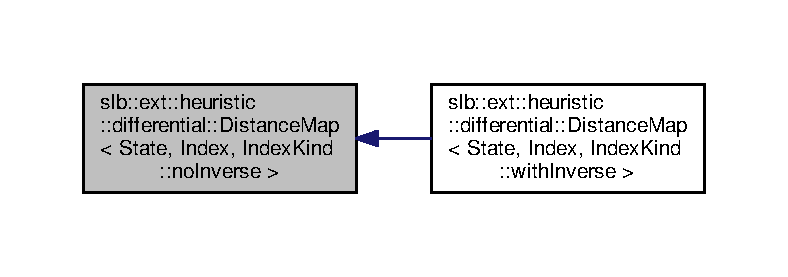
\includegraphics[width=350pt]{structslb_1_1ext_1_1heuristic_1_1differential_1_1DistanceMap_3_01State_00_01Index_00_01IndexKinde43ce932d9787cf913052e8d1057cce1}
\end{center}
\end{figure}
\subsubsection*{Public Types}
\begin{DoxyCompactItemize}
\item 
using \hyperlink{structslb_1_1ext_1_1heuristic_1_1differential_1_1DistanceMap_3_01State_00_01Index_00_01IndexKind_1_1noInverse_01_4_a9a67ddc91fe4ea5fbf6957d2105ed5a7}{Cost\+Type} = typename State\+::\+Cost\+Type\hypertarget{structslb_1_1ext_1_1heuristic_1_1differential_1_1DistanceMap_3_01State_00_01Index_00_01IndexKind_1_1noInverse_01_4_a9a67ddc91fe4ea5fbf6957d2105ed5a7}{}\label{structslb_1_1ext_1_1heuristic_1_1differential_1_1DistanceMap_3_01State_00_01Index_00_01IndexKind_1_1noInverse_01_4_a9a67ddc91fe4ea5fbf6957d2105ed5a7}

\begin{DoxyCompactList}\small\item\em The action cost type. \end{DoxyCompactList}\item 
using \hyperlink{structslb_1_1ext_1_1heuristic_1_1differential_1_1DistanceMap_3_01State_00_01Index_00_01IndexKind_1_1noInverse_01_4_acba898005faced74c6e3bf42c398f3d8}{Distances} = std\+::vector$<$ \hyperlink{structslb_1_1ext_1_1heuristic_1_1differential_1_1DistanceMap_3_01State_00_01Index_00_01IndexKind_1_1noInverse_01_4_a9a67ddc91fe4ea5fbf6957d2105ed5a7}{Cost\+Type} $>$\hypertarget{structslb_1_1ext_1_1heuristic_1_1differential_1_1DistanceMap_3_01State_00_01Index_00_01IndexKind_1_1noInverse_01_4_acba898005faced74c6e3bf42c398f3d8}{}\label{structslb_1_1ext_1_1heuristic_1_1differential_1_1DistanceMap_3_01State_00_01Index_00_01IndexKind_1_1noInverse_01_4_acba898005faced74c6e3bf42c398f3d8}

\begin{DoxyCompactList}\small\item\em The underlying type for storing distances to pivots. \end{DoxyCompactList}\end{DoxyCompactItemize}
\subsubsection*{Public Member Functions}
\begin{DoxyCompactItemize}
\item 
{\footnotesize template$<$class My\+Alg  = algorithm\+::\+Simple\+Uniform\+Cost$>$ }\\\hyperlink{structslb_1_1ext_1_1heuristic_1_1differential_1_1DistanceMap_3_01State_00_01Index_00_01IndexKind_1_1noInverse_01_4_aacdc18f08067c72e70fc47cbcda38994}{Distance\+Map} (const State \&s)
\begin{DoxyCompactList}\small\item\em The constructor. \end{DoxyCompactList}\item 
\hyperlink{structslb_1_1ext_1_1heuristic_1_1differential_1_1DistanceMap_3_01State_00_01Index_00_01IndexKind_1_1noInverse_01_4_a9a67ddc91fe4ea5fbf6957d2105ed5a7}{Cost\+Type} \hyperlink{structslb_1_1ext_1_1heuristic_1_1differential_1_1DistanceMap_3_01State_00_01Index_00_01IndexKind_1_1noInverse_01_4_ae7b3433931474cc6402ba6663495959b}{distance} (const State \&s) const 
\begin{DoxyCompactList}\small\item\em Returns the distance from the given state. \end{DoxyCompactList}\item 
int \hyperlink{structslb_1_1ext_1_1heuristic_1_1differential_1_1DistanceMap_3_01State_00_01Index_00_01IndexKind_1_1noInverse_01_4_a782b40376782f9ddcdade6257d3b7b37}{n\+States} () const 
\begin{DoxyCompactList}\small\item\em Returns the number of states from which distances are stored. \end{DoxyCompactList}\end{DoxyCompactItemize}
\subsubsection*{Protected Attributes}
\begin{DoxyCompactItemize}
\item 
\hyperlink{structslb_1_1ext_1_1heuristic_1_1differential_1_1DistanceMap_3_01State_00_01Index_00_01IndexKind_1_1noInverse_01_4_acba898005faced74c6e3bf42c398f3d8}{Distances} \hyperlink{structslb_1_1ext_1_1heuristic_1_1differential_1_1DistanceMap_3_01State_00_01Index_00_01IndexKind_1_1noInverse_01_4_a3ec407ff0436904399c1e4924694895e}{distances\+\_\+}\hypertarget{structslb_1_1ext_1_1heuristic_1_1differential_1_1DistanceMap_3_01State_00_01Index_00_01IndexKind_1_1noInverse_01_4_a3ec407ff0436904399c1e4924694895e}{}\label{structslb_1_1ext_1_1heuristic_1_1differential_1_1DistanceMap_3_01State_00_01Index_00_01IndexKind_1_1noInverse_01_4_a3ec407ff0436904399c1e4924694895e}

\begin{DoxyCompactList}\small\item\em The stored distances. \end{DoxyCompactList}\item 
int \hyperlink{structslb_1_1ext_1_1heuristic_1_1differential_1_1DistanceMap_3_01State_00_01Index_00_01IndexKind_1_1noInverse_01_4_a218e5e9f9b895c79139cd04f6f4603c7}{n\+States\+\_\+}\hypertarget{structslb_1_1ext_1_1heuristic_1_1differential_1_1DistanceMap_3_01State_00_01Index_00_01IndexKind_1_1noInverse_01_4_a218e5e9f9b895c79139cd04f6f4603c7}{}\label{structslb_1_1ext_1_1heuristic_1_1differential_1_1DistanceMap_3_01State_00_01Index_00_01IndexKind_1_1noInverse_01_4_a218e5e9f9b895c79139cd04f6f4603c7}

\begin{DoxyCompactList}\small\item\em the number of states from which distances are stored. \end{DoxyCompactList}\end{DoxyCompactItemize}


\subsubsection{Detailed Description}
\subsubsection*{template$<$class State, class Index$>$\\*
struct slb\+::ext\+::heuristic\+::differential\+::\+Distance\+Map$<$ State, Index, Index\+Kind\+::no\+Inverse $>$}

The type for storing distances to pivots. This specialization is for an index function without an inverse. 


\begin{DoxyTemplParams}{Template Parameters}
{\em State} & The state type representing the search domain. \\
\hline
{\em Index} & Mapping of states to indices. \\
\hline
{\em Index\+Kind} & The type denoting the kind of index. \\
\hline
\end{DoxyTemplParams}


Definition at line 33 of file distance\+\_\+map.\+h.



\subsubsection{Constructor \& Destructor Documentation}
\index{slb\+::ext\+::heuristic\+::differential\+::\+Distance\+Map$<$ State, Index, Index\+Kind\+::no\+Inverse $>$@{slb\+::ext\+::heuristic\+::differential\+::\+Distance\+Map$<$ State, Index, Index\+Kind\+::no\+Inverse $>$}!Distance\+Map@{Distance\+Map}}
\index{Distance\+Map@{Distance\+Map}!slb\+::ext\+::heuristic\+::differential\+::\+Distance\+Map$<$ State, Index, Index\+Kind\+::no\+Inverse $>$@{slb\+::ext\+::heuristic\+::differential\+::\+Distance\+Map$<$ State, Index, Index\+Kind\+::no\+Inverse $>$}}
\paragraph[{\texorpdfstring{Distance\+Map(const State \&s)}{DistanceMap(const State &s)}}]{\setlength{\rightskip}{0pt plus 5cm}template$<$class State , class Index $>$ template$<$class My\+Alg  = algorithm\+::\+Simple\+Uniform\+Cost$>$ {\bf slb\+::ext\+::heuristic\+::differential\+::\+Distance\+Map}$<$ State, Index, Index\+Kind\+::no\+Inverse $>$\+::{\bf Distance\+Map} (
\begin{DoxyParamCaption}
\item[{const State \&}]{s}
\end{DoxyParamCaption}
)\hspace{0.3cm}{\ttfamily [inline]}}\hypertarget{structslb_1_1ext_1_1heuristic_1_1differential_1_1DistanceMap_3_01State_00_01Index_00_01IndexKind_1_1noInverse_01_4_aacdc18f08067c72e70fc47cbcda38994}{}\label{structslb_1_1ext_1_1heuristic_1_1differential_1_1DistanceMap_3_01State_00_01Index_00_01IndexKind_1_1noInverse_01_4_aacdc18f08067c72e70fc47cbcda38994}


The constructor. 


\begin{DoxyTemplParams}{Template Parameters}
{\em My\+Alg} & The algorithm to be used to find distances to the specified state. \\
\hline
\end{DoxyTemplParams}

\begin{DoxyParams}{Parameters}
{\em s} & The state to which distances are to be stored. \\
\hline
\end{DoxyParams}


Definition at line 45 of file distance\+\_\+map.\+h.



\subsubsection{Member Function Documentation}
\index{slb\+::ext\+::heuristic\+::differential\+::\+Distance\+Map$<$ State, Index, Index\+Kind\+::no\+Inverse $>$@{slb\+::ext\+::heuristic\+::differential\+::\+Distance\+Map$<$ State, Index, Index\+Kind\+::no\+Inverse $>$}!distance@{distance}}
\index{distance@{distance}!slb\+::ext\+::heuristic\+::differential\+::\+Distance\+Map$<$ State, Index, Index\+Kind\+::no\+Inverse $>$@{slb\+::ext\+::heuristic\+::differential\+::\+Distance\+Map$<$ State, Index, Index\+Kind\+::no\+Inverse $>$}}
\paragraph[{\texorpdfstring{distance(const State \&s) const }{distance(const State &s) const }}]{\setlength{\rightskip}{0pt plus 5cm}template$<$class State , class Index $>$ {\bf Cost\+Type} {\bf slb\+::ext\+::heuristic\+::differential\+::\+Distance\+Map}$<$ State, Index, Index\+Kind\+::no\+Inverse $>$\+::distance (
\begin{DoxyParamCaption}
\item[{const State \&}]{s}
\end{DoxyParamCaption}
) const\hspace{0.3cm}{\ttfamily [inline]}}\hypertarget{structslb_1_1ext_1_1heuristic_1_1differential_1_1DistanceMap_3_01State_00_01Index_00_01IndexKind_1_1noInverse_01_4_ae7b3433931474cc6402ba6663495959b}{}\label{structslb_1_1ext_1_1heuristic_1_1differential_1_1DistanceMap_3_01State_00_01Index_00_01IndexKind_1_1noInverse_01_4_ae7b3433931474cc6402ba6663495959b}


Returns the distance from the given state. 


\begin{DoxyParams}{Parameters}
{\em s} & The state of interest. \\
\hline
\end{DoxyParams}
\begin{DoxyReturn}{Returns}
The distance from {\ttfamily s}. 
\end{DoxyReturn}


Definition at line 58 of file distance\+\_\+map.\+h.

\index{slb\+::ext\+::heuristic\+::differential\+::\+Distance\+Map$<$ State, Index, Index\+Kind\+::no\+Inverse $>$@{slb\+::ext\+::heuristic\+::differential\+::\+Distance\+Map$<$ State, Index, Index\+Kind\+::no\+Inverse $>$}!n\+States@{n\+States}}
\index{n\+States@{n\+States}!slb\+::ext\+::heuristic\+::differential\+::\+Distance\+Map$<$ State, Index, Index\+Kind\+::no\+Inverse $>$@{slb\+::ext\+::heuristic\+::differential\+::\+Distance\+Map$<$ State, Index, Index\+Kind\+::no\+Inverse $>$}}
\paragraph[{\texorpdfstring{n\+States() const }{nStates() const }}]{\setlength{\rightskip}{0pt plus 5cm}template$<$class State , class Index $>$ int {\bf slb\+::ext\+::heuristic\+::differential\+::\+Distance\+Map}$<$ State, Index, Index\+Kind\+::no\+Inverse $>$\+::n\+States (
\begin{DoxyParamCaption}
{}
\end{DoxyParamCaption}
) const\hspace{0.3cm}{\ttfamily [inline]}}\hypertarget{structslb_1_1ext_1_1heuristic_1_1differential_1_1DistanceMap_3_01State_00_01Index_00_01IndexKind_1_1noInverse_01_4_a782b40376782f9ddcdade6257d3b7b37}{}\label{structslb_1_1ext_1_1heuristic_1_1differential_1_1DistanceMap_3_01State_00_01Index_00_01IndexKind_1_1noInverse_01_4_a782b40376782f9ddcdade6257d3b7b37}


Returns the number of states from which distances are stored. 

\begin{DoxyReturn}{Returns}
The number of states from which distances are stored. 
\end{DoxyReturn}


Definition at line 62 of file distance\+\_\+map.\+h.



The documentation for this struct was generated from the following file\+:\begin{DoxyCompactItemize}
\item 
extensions/heuristics/differential/\hyperlink{distance__map_8h}{distance\+\_\+map.\+h}\end{DoxyCompactItemize}

\hypertarget{structslb_1_1ext_1_1heuristic_1_1differential_1_1DistanceMap_3_01State_00_01Index_00_01IndexKind_1_1none_01_4}{}\subsection{slb\+:\+:ext\+:\+:heuristic\+:\+:differential\+:\+:Distance\+Map$<$ State, Index, Index\+Kind\+:\+:none $>$ Struct Template Reference}
\label{structslb_1_1ext_1_1heuristic_1_1differential_1_1DistanceMap_3_01State_00_01Index_00_01IndexKind_1_1none_01_4}\index{slb\+::ext\+::heuristic\+::differential\+::\+Distance\+Map$<$ State, Index, Index\+Kind\+::none $>$@{slb\+::ext\+::heuristic\+::differential\+::\+Distance\+Map$<$ State, Index, Index\+Kind\+::none $>$}}


The type for storing distances to pivots. This specialization is for the situation without an index.  




{\ttfamily \#include $<$distance\+\_\+map.\+h$>$}

\subsubsection*{Public Types}
\begin{DoxyCompactItemize}
\item 
using \hyperlink{structslb_1_1ext_1_1heuristic_1_1differential_1_1DistanceMap_3_01State_00_01Index_00_01IndexKind_1_1none_01_4_a7b581d785190b93a68423219d1e39b35}{Cost\+Type} = typename State\+::\+Cost\+Type\hypertarget{structslb_1_1ext_1_1heuristic_1_1differential_1_1DistanceMap_3_01State_00_01Index_00_01IndexKind_1_1none_01_4_a7b581d785190b93a68423219d1e39b35}{}\label{structslb_1_1ext_1_1heuristic_1_1differential_1_1DistanceMap_3_01State_00_01Index_00_01IndexKind_1_1none_01_4_a7b581d785190b93a68423219d1e39b35}

\begin{DoxyCompactList}\small\item\em The action cost type. \end{DoxyCompactList}\item 
using \hyperlink{structslb_1_1ext_1_1heuristic_1_1differential_1_1DistanceMap_3_01State_00_01Index_00_01IndexKind_1_1none_01_4_a41fb62a9e902a7786b604a806317ac47}{Distances} = std\+::unordered\+\_\+map$<$ State, \hyperlink{structslb_1_1ext_1_1heuristic_1_1differential_1_1DistanceMap_3_01State_00_01Index_00_01IndexKind_1_1none_01_4_a7b581d785190b93a68423219d1e39b35}{Cost\+Type}, \hyperlink{structslb_1_1core_1_1util_1_1StateHash}{core\+::util\+::\+State\+Hash}$<$ State $>$$>$\hypertarget{structslb_1_1ext_1_1heuristic_1_1differential_1_1DistanceMap_3_01State_00_01Index_00_01IndexKind_1_1none_01_4_a41fb62a9e902a7786b604a806317ac47}{}\label{structslb_1_1ext_1_1heuristic_1_1differential_1_1DistanceMap_3_01State_00_01Index_00_01IndexKind_1_1none_01_4_a41fb62a9e902a7786b604a806317ac47}

\begin{DoxyCompactList}\small\item\em The underlying type for storing distances to pivots. \end{DoxyCompactList}\item 
using \hyperlink{structslb_1_1ext_1_1heuristic_1_1differential_1_1DistanceMap_3_01State_00_01Index_00_01IndexKind_1_1none_01_4_ab5a07fc5da2680acfe08b598844a065d}{Iterator} = \hyperlink{structslb_1_1core_1_1util_1_1MapKeyIterator}{core\+::util\+::\+Map\+Key\+Iterator}$<$ \hyperlink{structslb_1_1ext_1_1heuristic_1_1differential_1_1DistanceMap_3_01State_00_01Index_00_01IndexKind_1_1none_01_4_a41fb62a9e902a7786b604a806317ac47}{Distances} $>$\hypertarget{structslb_1_1ext_1_1heuristic_1_1differential_1_1DistanceMap_3_01State_00_01Index_00_01IndexKind_1_1none_01_4_ab5a07fc5da2680acfe08b598844a065d}{}\label{structslb_1_1ext_1_1heuristic_1_1differential_1_1DistanceMap_3_01State_00_01Index_00_01IndexKind_1_1none_01_4_ab5a07fc5da2680acfe08b598844a065d}

\begin{DoxyCompactList}\small\item\em The iterator for the distances. \end{DoxyCompactList}\item 
using \hyperlink{structslb_1_1ext_1_1heuristic_1_1differential_1_1DistanceMap_3_01State_00_01Index_00_01IndexKind_1_1none_01_4_a3a019e07ed97eaea1e42ffc7d39e03d7}{Const\+Iterator} = \hyperlink{structslb_1_1core_1_1util_1_1MapKeyConstIterator}{core\+::util\+::\+Map\+Key\+Const\+Iterator}$<$ \hyperlink{structslb_1_1ext_1_1heuristic_1_1differential_1_1DistanceMap_3_01State_00_01Index_00_01IndexKind_1_1none_01_4_a41fb62a9e902a7786b604a806317ac47}{Distances} $>$\hypertarget{structslb_1_1ext_1_1heuristic_1_1differential_1_1DistanceMap_3_01State_00_01Index_00_01IndexKind_1_1none_01_4_a3a019e07ed97eaea1e42ffc7d39e03d7}{}\label{structslb_1_1ext_1_1heuristic_1_1differential_1_1DistanceMap_3_01State_00_01Index_00_01IndexKind_1_1none_01_4_a3a019e07ed97eaea1e42ffc7d39e03d7}

\begin{DoxyCompactList}\small\item\em The constant iterator for the distances. \end{DoxyCompactList}\end{DoxyCompactItemize}
\subsubsection*{Public Member Functions}
\begin{DoxyCompactItemize}
\item 
\hyperlink{structslb_1_1ext_1_1heuristic_1_1differential_1_1DistanceMap_3_01State_00_01Index_00_01IndexKind_1_1none_01_4_ab5a07fc5da2680acfe08b598844a065d}{Iterator} \hyperlink{structslb_1_1ext_1_1heuristic_1_1differential_1_1DistanceMap_3_01State_00_01Index_00_01IndexKind_1_1none_01_4_a2eea88fd944da897af2b747930e1e759}{begin} ()
\begin{DoxyCompactList}\small\item\em Returns iterator to the beginning of the distances. \end{DoxyCompactList}\item 
\hyperlink{structslb_1_1ext_1_1heuristic_1_1differential_1_1DistanceMap_3_01State_00_01Index_00_01IndexKind_1_1none_01_4_a3a019e07ed97eaea1e42ffc7d39e03d7}{Const\+Iterator} \hyperlink{structslb_1_1ext_1_1heuristic_1_1differential_1_1DistanceMap_3_01State_00_01Index_00_01IndexKind_1_1none_01_4_a12ff1931fdbb60942309f0e04fdbe462}{begin} () const 
\begin{DoxyCompactList}\small\item\em Returns constant iterator to the beginning of the distances. \end{DoxyCompactList}\item 
\hyperlink{structslb_1_1ext_1_1heuristic_1_1differential_1_1DistanceMap_3_01State_00_01Index_00_01IndexKind_1_1none_01_4_ab5a07fc5da2680acfe08b598844a065d}{Iterator} \hyperlink{structslb_1_1ext_1_1heuristic_1_1differential_1_1DistanceMap_3_01State_00_01Index_00_01IndexKind_1_1none_01_4_a2fe7b4835665ee22009b5afdbc6de266}{end} ()
\begin{DoxyCompactList}\small\item\em Returns iterator to the end of the distances. \end{DoxyCompactList}\item 
\hyperlink{structslb_1_1ext_1_1heuristic_1_1differential_1_1DistanceMap_3_01State_00_01Index_00_01IndexKind_1_1none_01_4_a3a019e07ed97eaea1e42ffc7d39e03d7}{Const\+Iterator} \hyperlink{structslb_1_1ext_1_1heuristic_1_1differential_1_1DistanceMap_3_01State_00_01Index_00_01IndexKind_1_1none_01_4_a50c049933b5b704b413c0dc7f011c30c}{end} () const 
\begin{DoxyCompactList}\small\item\em Returns constant iterator to the end of the distances. \end{DoxyCompactList}\item 
{\footnotesize template$<$class It $>$ }\\State \hyperlink{structslb_1_1ext_1_1heuristic_1_1differential_1_1DistanceMap_3_01State_00_01Index_00_01IndexKind_1_1none_01_4_aa4a2bfeeb834d60af896ce17e323c13c}{it\+To\+State} (It it) const 
\begin{DoxyCompactList}\small\item\em Returns the state (from which a distance is stored) corresponding to the given iterator. \end{DoxyCompactList}\item 
{\footnotesize template$<$class My\+Alg  = algorithm\+::\+Simple\+Uniform\+Cost$>$ }\\\hyperlink{structslb_1_1ext_1_1heuristic_1_1differential_1_1DistanceMap_3_01State_00_01Index_00_01IndexKind_1_1none_01_4_a2f24c0038c0063c1efb23558a981bb30}{Distance\+Map} (const State \&s)
\begin{DoxyCompactList}\small\item\em The constructor. \end{DoxyCompactList}\item 
\hyperlink{structslb_1_1ext_1_1heuristic_1_1differential_1_1DistanceMap_3_01State_00_01Index_00_01IndexKind_1_1none_01_4_a7b581d785190b93a68423219d1e39b35}{Cost\+Type} \hyperlink{structslb_1_1ext_1_1heuristic_1_1differential_1_1DistanceMap_3_01State_00_01Index_00_01IndexKind_1_1none_01_4_a7512d3c098d50eeb82974c8c4464683e}{distance} (const State \&s) const 
\begin{DoxyCompactList}\small\item\em Returns the distance from the given state. \end{DoxyCompactList}\item 
{\footnotesize template$<$class Distances1 $>$ }\\void \hyperlink{structslb_1_1ext_1_1heuristic_1_1differential_1_1DistanceMap_3_01State_00_01Index_00_01IndexKind_1_1none_01_4_a6186c3704378a67d22382b0f41f55cb2}{intersect} (const Distances1 \&d)
\begin{DoxyCompactList}\small\item\em Computes the minimum of each stored distance and the corresponding distance given by the argument. \end{DoxyCompactList}\item 
State \hyperlink{structslb_1_1ext_1_1heuristic_1_1differential_1_1DistanceMap_3_01State_00_01Index_00_01IndexKind_1_1none_01_4_a1ef6298a4d0ee2096e4d0b640857a813}{farthest} () const 
\begin{DoxyCompactList}\small\item\em Returns the state from which the distance is maximal. \end{DoxyCompactList}\item 
const \hyperlink{structslb_1_1ext_1_1heuristic_1_1differential_1_1DistanceMap_3_01State_00_01Index_00_01IndexKind_1_1none_01_4_a41fb62a9e902a7786b604a806317ac47}{Distances} \& \hyperlink{structslb_1_1ext_1_1heuristic_1_1differential_1_1DistanceMap_3_01State_00_01Index_00_01IndexKind_1_1none_01_4_af26fe94fd1f7774eaccc4f085c04603f}{distance\+Map} () const 
\begin{DoxyCompactList}\small\item\em Returns the raw distances. \end{DoxyCompactList}\item 
int \hyperlink{structslb_1_1ext_1_1heuristic_1_1differential_1_1DistanceMap_3_01State_00_01Index_00_01IndexKind_1_1none_01_4_a339a4cd0f26c792b27f4f07c0b9db335}{n\+States} () const 
\begin{DoxyCompactList}\small\item\em Returns the number of states from which distances are stored. \end{DoxyCompactList}\end{DoxyCompactItemize}
\subsubsection*{Protected Attributes}
\begin{DoxyCompactItemize}
\item 
\hyperlink{structslb_1_1ext_1_1heuristic_1_1differential_1_1DistanceMap_3_01State_00_01Index_00_01IndexKind_1_1none_01_4_a41fb62a9e902a7786b604a806317ac47}{Distances} \hyperlink{structslb_1_1ext_1_1heuristic_1_1differential_1_1DistanceMap_3_01State_00_01Index_00_01IndexKind_1_1none_01_4_a878e5bbd052dd9c39fcfa60c528cdf24}{distances\+\_\+}\hypertarget{structslb_1_1ext_1_1heuristic_1_1differential_1_1DistanceMap_3_01State_00_01Index_00_01IndexKind_1_1none_01_4_a878e5bbd052dd9c39fcfa60c528cdf24}{}\label{structslb_1_1ext_1_1heuristic_1_1differential_1_1DistanceMap_3_01State_00_01Index_00_01IndexKind_1_1none_01_4_a878e5bbd052dd9c39fcfa60c528cdf24}

\begin{DoxyCompactList}\small\item\em The stored distances. \end{DoxyCompactList}\item 
int \hyperlink{structslb_1_1ext_1_1heuristic_1_1differential_1_1DistanceMap_3_01State_00_01Index_00_01IndexKind_1_1none_01_4_a0ef73098766ead44e477377fefaa648a}{n\+States\+\_\+}\hypertarget{structslb_1_1ext_1_1heuristic_1_1differential_1_1DistanceMap_3_01State_00_01Index_00_01IndexKind_1_1none_01_4_a0ef73098766ead44e477377fefaa648a}{}\label{structslb_1_1ext_1_1heuristic_1_1differential_1_1DistanceMap_3_01State_00_01Index_00_01IndexKind_1_1none_01_4_a0ef73098766ead44e477377fefaa648a}

\begin{DoxyCompactList}\small\item\em the number of states from which distances are stored. \end{DoxyCompactList}\end{DoxyCompactItemize}


\subsubsection{Detailed Description}
\subsubsection*{template$<$class State, class Index$>$\\*
struct slb\+::ext\+::heuristic\+::differential\+::\+Distance\+Map$<$ State, Index, Index\+Kind\+::none $>$}

The type for storing distances to pivots. This specialization is for the situation without an index. 


\begin{DoxyTemplParams}{Template Parameters}
{\em State} & The state type representing the search domain. \\
\hline
{\em Index} & Mapping of states to indices. \\
\hline
{\em Index\+Kind} & The type denoting the kind of index. \\
\hline
\end{DoxyTemplParams}


Definition at line 154 of file distance\+\_\+map.\+h.



\subsubsection{Constructor \& Destructor Documentation}
\index{slb\+::ext\+::heuristic\+::differential\+::\+Distance\+Map$<$ State, Index, Index\+Kind\+::none $>$@{slb\+::ext\+::heuristic\+::differential\+::\+Distance\+Map$<$ State, Index, Index\+Kind\+::none $>$}!Distance\+Map@{Distance\+Map}}
\index{Distance\+Map@{Distance\+Map}!slb\+::ext\+::heuristic\+::differential\+::\+Distance\+Map$<$ State, Index, Index\+Kind\+::none $>$@{slb\+::ext\+::heuristic\+::differential\+::\+Distance\+Map$<$ State, Index, Index\+Kind\+::none $>$}}
\paragraph[{\texorpdfstring{Distance\+Map(const State \&s)}{DistanceMap(const State &s)}}]{\setlength{\rightskip}{0pt plus 5cm}template$<$class State , class Index $>$ template$<$class My\+Alg  = algorithm\+::\+Simple\+Uniform\+Cost$>$ {\bf slb\+::ext\+::heuristic\+::differential\+::\+Distance\+Map}$<$ State, Index, Index\+Kind\+::none $>$\+::{\bf Distance\+Map} (
\begin{DoxyParamCaption}
\item[{const State \&}]{s}
\end{DoxyParamCaption}
)\hspace{0.3cm}{\ttfamily [inline]}}\hypertarget{structslb_1_1ext_1_1heuristic_1_1differential_1_1DistanceMap_3_01State_00_01Index_00_01IndexKind_1_1none_01_4_a2f24c0038c0063c1efb23558a981bb30}{}\label{structslb_1_1ext_1_1heuristic_1_1differential_1_1DistanceMap_3_01State_00_01Index_00_01IndexKind_1_1none_01_4_a2f24c0038c0063c1efb23558a981bb30}


The constructor. 


\begin{DoxyTemplParams}{Template Parameters}
{\em My\+Alg} & The algorithm to be used to find distances to the specified state. \\
\hline
\end{DoxyTemplParams}

\begin{DoxyParams}{Parameters}
{\em s} & The state to which distances are to be stored. \\
\hline
\end{DoxyParams}


Definition at line 197 of file distance\+\_\+map.\+h.



\subsubsection{Member Function Documentation}
\index{slb\+::ext\+::heuristic\+::differential\+::\+Distance\+Map$<$ State, Index, Index\+Kind\+::none $>$@{slb\+::ext\+::heuristic\+::differential\+::\+Distance\+Map$<$ State, Index, Index\+Kind\+::none $>$}!begin@{begin}}
\index{begin@{begin}!slb\+::ext\+::heuristic\+::differential\+::\+Distance\+Map$<$ State, Index, Index\+Kind\+::none $>$@{slb\+::ext\+::heuristic\+::differential\+::\+Distance\+Map$<$ State, Index, Index\+Kind\+::none $>$}}
\paragraph[{\texorpdfstring{begin()}{begin()}}]{\setlength{\rightskip}{0pt plus 5cm}template$<$class State , class Index $>$ {\bf Iterator} {\bf slb\+::ext\+::heuristic\+::differential\+::\+Distance\+Map}$<$ State, Index, Index\+Kind\+::none $>$\+::begin (
\begin{DoxyParamCaption}
{}
\end{DoxyParamCaption}
)\hspace{0.3cm}{\ttfamily [inline]}}\hypertarget{structslb_1_1ext_1_1heuristic_1_1differential_1_1DistanceMap_3_01State_00_01Index_00_01IndexKind_1_1none_01_4_a2eea88fd944da897af2b747930e1e759}{}\label{structslb_1_1ext_1_1heuristic_1_1differential_1_1DistanceMap_3_01State_00_01Index_00_01IndexKind_1_1none_01_4_a2eea88fd944da897af2b747930e1e759}


Returns iterator to the beginning of the distances. 

\begin{DoxyReturn}{Returns}
Iterator to the beginning of the distances. 
\end{DoxyReturn}


Definition at line 170 of file distance\+\_\+map.\+h.

\index{slb\+::ext\+::heuristic\+::differential\+::\+Distance\+Map$<$ State, Index, Index\+Kind\+::none $>$@{slb\+::ext\+::heuristic\+::differential\+::\+Distance\+Map$<$ State, Index, Index\+Kind\+::none $>$}!begin@{begin}}
\index{begin@{begin}!slb\+::ext\+::heuristic\+::differential\+::\+Distance\+Map$<$ State, Index, Index\+Kind\+::none $>$@{slb\+::ext\+::heuristic\+::differential\+::\+Distance\+Map$<$ State, Index, Index\+Kind\+::none $>$}}
\paragraph[{\texorpdfstring{begin() const }{begin() const }}]{\setlength{\rightskip}{0pt plus 5cm}template$<$class State , class Index $>$ {\bf Const\+Iterator} {\bf slb\+::ext\+::heuristic\+::differential\+::\+Distance\+Map}$<$ State, Index, Index\+Kind\+::none $>$\+::begin (
\begin{DoxyParamCaption}
{}
\end{DoxyParamCaption}
) const\hspace{0.3cm}{\ttfamily [inline]}}\hypertarget{structslb_1_1ext_1_1heuristic_1_1differential_1_1DistanceMap_3_01State_00_01Index_00_01IndexKind_1_1none_01_4_a12ff1931fdbb60942309f0e04fdbe462}{}\label{structslb_1_1ext_1_1heuristic_1_1differential_1_1DistanceMap_3_01State_00_01Index_00_01IndexKind_1_1none_01_4_a12ff1931fdbb60942309f0e04fdbe462}


Returns constant iterator to the beginning of the distances. 

\begin{DoxyReturn}{Returns}
Constant iterator to the beginning of the distances. 
\end{DoxyReturn}


Definition at line 174 of file distance\+\_\+map.\+h.

\index{slb\+::ext\+::heuristic\+::differential\+::\+Distance\+Map$<$ State, Index, Index\+Kind\+::none $>$@{slb\+::ext\+::heuristic\+::differential\+::\+Distance\+Map$<$ State, Index, Index\+Kind\+::none $>$}!distance@{distance}}
\index{distance@{distance}!slb\+::ext\+::heuristic\+::differential\+::\+Distance\+Map$<$ State, Index, Index\+Kind\+::none $>$@{slb\+::ext\+::heuristic\+::differential\+::\+Distance\+Map$<$ State, Index, Index\+Kind\+::none $>$}}
\paragraph[{\texorpdfstring{distance(const State \&s) const }{distance(const State &s) const }}]{\setlength{\rightskip}{0pt plus 5cm}template$<$class State , class Index $>$ {\bf Cost\+Type} {\bf slb\+::ext\+::heuristic\+::differential\+::\+Distance\+Map}$<$ State, Index, Index\+Kind\+::none $>$\+::distance (
\begin{DoxyParamCaption}
\item[{const State \&}]{s}
\end{DoxyParamCaption}
) const\hspace{0.3cm}{\ttfamily [inline]}}\hypertarget{structslb_1_1ext_1_1heuristic_1_1differential_1_1DistanceMap_3_01State_00_01Index_00_01IndexKind_1_1none_01_4_a7512d3c098d50eeb82974c8c4464683e}{}\label{structslb_1_1ext_1_1heuristic_1_1differential_1_1DistanceMap_3_01State_00_01Index_00_01IndexKind_1_1none_01_4_a7512d3c098d50eeb82974c8c4464683e}


Returns the distance from the given state. 


\begin{DoxyParams}{Parameters}
{\em s} & The state of interest. \\
\hline
\end{DoxyParams}
\begin{DoxyReturn}{Returns}
The distance from {\ttfamily s}. 
\end{DoxyReturn}


Definition at line 205 of file distance\+\_\+map.\+h.

\index{slb\+::ext\+::heuristic\+::differential\+::\+Distance\+Map$<$ State, Index, Index\+Kind\+::none $>$@{slb\+::ext\+::heuristic\+::differential\+::\+Distance\+Map$<$ State, Index, Index\+Kind\+::none $>$}!distance\+Map@{distance\+Map}}
\index{distance\+Map@{distance\+Map}!slb\+::ext\+::heuristic\+::differential\+::\+Distance\+Map$<$ State, Index, Index\+Kind\+::none $>$@{slb\+::ext\+::heuristic\+::differential\+::\+Distance\+Map$<$ State, Index, Index\+Kind\+::none $>$}}
\paragraph[{\texorpdfstring{distance\+Map() const }{distanceMap() const }}]{\setlength{\rightskip}{0pt plus 5cm}template$<$class State , class Index $>$ const {\bf Distances}\& {\bf slb\+::ext\+::heuristic\+::differential\+::\+Distance\+Map}$<$ State, Index, Index\+Kind\+::none $>$\+::distance\+Map (
\begin{DoxyParamCaption}
{}
\end{DoxyParamCaption}
) const\hspace{0.3cm}{\ttfamily [inline]}}\hypertarget{structslb_1_1ext_1_1heuristic_1_1differential_1_1DistanceMap_3_01State_00_01Index_00_01IndexKind_1_1none_01_4_af26fe94fd1f7774eaccc4f085c04603f}{}\label{structslb_1_1ext_1_1heuristic_1_1differential_1_1DistanceMap_3_01State_00_01Index_00_01IndexKind_1_1none_01_4_af26fe94fd1f7774eaccc4f085c04603f}


Returns the raw distances. 

\begin{DoxyReturn}{Returns}
The raw distances. 
\end{DoxyReturn}


Definition at line 227 of file distance\+\_\+map.\+h.

\index{slb\+::ext\+::heuristic\+::differential\+::\+Distance\+Map$<$ State, Index, Index\+Kind\+::none $>$@{slb\+::ext\+::heuristic\+::differential\+::\+Distance\+Map$<$ State, Index, Index\+Kind\+::none $>$}!end@{end}}
\index{end@{end}!slb\+::ext\+::heuristic\+::differential\+::\+Distance\+Map$<$ State, Index, Index\+Kind\+::none $>$@{slb\+::ext\+::heuristic\+::differential\+::\+Distance\+Map$<$ State, Index, Index\+Kind\+::none $>$}}
\paragraph[{\texorpdfstring{end()}{end()}}]{\setlength{\rightskip}{0pt plus 5cm}template$<$class State , class Index $>$ {\bf Iterator} {\bf slb\+::ext\+::heuristic\+::differential\+::\+Distance\+Map}$<$ State, Index, Index\+Kind\+::none $>$\+::end (
\begin{DoxyParamCaption}
{}
\end{DoxyParamCaption}
)\hspace{0.3cm}{\ttfamily [inline]}}\hypertarget{structslb_1_1ext_1_1heuristic_1_1differential_1_1DistanceMap_3_01State_00_01Index_00_01IndexKind_1_1none_01_4_a2fe7b4835665ee22009b5afdbc6de266}{}\label{structslb_1_1ext_1_1heuristic_1_1differential_1_1DistanceMap_3_01State_00_01Index_00_01IndexKind_1_1none_01_4_a2fe7b4835665ee22009b5afdbc6de266}


Returns iterator to the end of the distances. 

\begin{DoxyReturn}{Returns}
Iterator to the end of the distances. 
\end{DoxyReturn}


Definition at line 178 of file distance\+\_\+map.\+h.

\index{slb\+::ext\+::heuristic\+::differential\+::\+Distance\+Map$<$ State, Index, Index\+Kind\+::none $>$@{slb\+::ext\+::heuristic\+::differential\+::\+Distance\+Map$<$ State, Index, Index\+Kind\+::none $>$}!end@{end}}
\index{end@{end}!slb\+::ext\+::heuristic\+::differential\+::\+Distance\+Map$<$ State, Index, Index\+Kind\+::none $>$@{slb\+::ext\+::heuristic\+::differential\+::\+Distance\+Map$<$ State, Index, Index\+Kind\+::none $>$}}
\paragraph[{\texorpdfstring{end() const }{end() const }}]{\setlength{\rightskip}{0pt plus 5cm}template$<$class State , class Index $>$ {\bf Const\+Iterator} {\bf slb\+::ext\+::heuristic\+::differential\+::\+Distance\+Map}$<$ State, Index, Index\+Kind\+::none $>$\+::end (
\begin{DoxyParamCaption}
{}
\end{DoxyParamCaption}
) const\hspace{0.3cm}{\ttfamily [inline]}}\hypertarget{structslb_1_1ext_1_1heuristic_1_1differential_1_1DistanceMap_3_01State_00_01Index_00_01IndexKind_1_1none_01_4_a50c049933b5b704b413c0dc7f011c30c}{}\label{structslb_1_1ext_1_1heuristic_1_1differential_1_1DistanceMap_3_01State_00_01Index_00_01IndexKind_1_1none_01_4_a50c049933b5b704b413c0dc7f011c30c}


Returns constant iterator to the end of the distances. 

\begin{DoxyReturn}{Returns}
Constant iterator to the end of the distances. 
\end{DoxyReturn}


Definition at line 182 of file distance\+\_\+map.\+h.

\index{slb\+::ext\+::heuristic\+::differential\+::\+Distance\+Map$<$ State, Index, Index\+Kind\+::none $>$@{slb\+::ext\+::heuristic\+::differential\+::\+Distance\+Map$<$ State, Index, Index\+Kind\+::none $>$}!farthest@{farthest}}
\index{farthest@{farthest}!slb\+::ext\+::heuristic\+::differential\+::\+Distance\+Map$<$ State, Index, Index\+Kind\+::none $>$@{slb\+::ext\+::heuristic\+::differential\+::\+Distance\+Map$<$ State, Index, Index\+Kind\+::none $>$}}
\paragraph[{\texorpdfstring{farthest() const }{farthest() const }}]{\setlength{\rightskip}{0pt plus 5cm}template$<$class State , class Index $>$ State {\bf slb\+::ext\+::heuristic\+::differential\+::\+Distance\+Map}$<$ State, Index, Index\+Kind\+::none $>$\+::farthest (
\begin{DoxyParamCaption}
{}
\end{DoxyParamCaption}
) const\hspace{0.3cm}{\ttfamily [inline]}}\hypertarget{structslb_1_1ext_1_1heuristic_1_1differential_1_1DistanceMap_3_01State_00_01Index_00_01IndexKind_1_1none_01_4_a1ef6298a4d0ee2096e4d0b640857a813}{}\label{structslb_1_1ext_1_1heuristic_1_1differential_1_1DistanceMap_3_01State_00_01Index_00_01IndexKind_1_1none_01_4_a1ef6298a4d0ee2096e4d0b640857a813}


Returns the state from which the distance is maximal. 

\begin{DoxyReturn}{Returns}
The state from which the distance is maximal. 
\end{DoxyReturn}


Definition at line 223 of file distance\+\_\+map.\+h.

\index{slb\+::ext\+::heuristic\+::differential\+::\+Distance\+Map$<$ State, Index, Index\+Kind\+::none $>$@{slb\+::ext\+::heuristic\+::differential\+::\+Distance\+Map$<$ State, Index, Index\+Kind\+::none $>$}!intersect@{intersect}}
\index{intersect@{intersect}!slb\+::ext\+::heuristic\+::differential\+::\+Distance\+Map$<$ State, Index, Index\+Kind\+::none $>$@{slb\+::ext\+::heuristic\+::differential\+::\+Distance\+Map$<$ State, Index, Index\+Kind\+::none $>$}}
\paragraph[{\texorpdfstring{intersect(const Distances1 \&d)}{intersect(const Distances1 &d)}}]{\setlength{\rightskip}{0pt plus 5cm}template$<$class State , class Index $>$ template$<$class Distances1 $>$ void {\bf slb\+::ext\+::heuristic\+::differential\+::\+Distance\+Map}$<$ State, Index, Index\+Kind\+::none $>$\+::intersect (
\begin{DoxyParamCaption}
\item[{const Distances1 \&}]{d}
\end{DoxyParamCaption}
)\hspace{0.3cm}{\ttfamily [inline]}}\hypertarget{structslb_1_1ext_1_1heuristic_1_1differential_1_1DistanceMap_3_01State_00_01Index_00_01IndexKind_1_1none_01_4_a6186c3704378a67d22382b0f41f55cb2}{}\label{structslb_1_1ext_1_1heuristic_1_1differential_1_1DistanceMap_3_01State_00_01Index_00_01IndexKind_1_1none_01_4_a6186c3704378a67d22382b0f41f55cb2}


Computes the minimum of each stored distance and the corresponding distance given by the argument. 


\begin{DoxyTemplParams}{Template Parameters}
{\em Distances1} & The type for the distances given by the argument. \\
\hline
\end{DoxyTemplParams}

\begin{DoxyParams}{Parameters}
{\em d} & The given distances. \\
\hline
\end{DoxyParams}


Definition at line 216 of file distance\+\_\+map.\+h.

\index{slb\+::ext\+::heuristic\+::differential\+::\+Distance\+Map$<$ State, Index, Index\+Kind\+::none $>$@{slb\+::ext\+::heuristic\+::differential\+::\+Distance\+Map$<$ State, Index, Index\+Kind\+::none $>$}!it\+To\+State@{it\+To\+State}}
\index{it\+To\+State@{it\+To\+State}!slb\+::ext\+::heuristic\+::differential\+::\+Distance\+Map$<$ State, Index, Index\+Kind\+::none $>$@{slb\+::ext\+::heuristic\+::differential\+::\+Distance\+Map$<$ State, Index, Index\+Kind\+::none $>$}}
\paragraph[{\texorpdfstring{it\+To\+State(\+It it) const }{itToState(It it) const }}]{\setlength{\rightskip}{0pt plus 5cm}template$<$class State , class Index $>$ template$<$class It $>$ State {\bf slb\+::ext\+::heuristic\+::differential\+::\+Distance\+Map}$<$ State, Index, Index\+Kind\+::none $>$\+::it\+To\+State (
\begin{DoxyParamCaption}
\item[{It}]{it}
\end{DoxyParamCaption}
) const\hspace{0.3cm}{\ttfamily [inline]}}\hypertarget{structslb_1_1ext_1_1heuristic_1_1differential_1_1DistanceMap_3_01State_00_01Index_00_01IndexKind_1_1none_01_4_aa4a2bfeeb834d60af896ce17e323c13c}{}\label{structslb_1_1ext_1_1heuristic_1_1differential_1_1DistanceMap_3_01State_00_01Index_00_01IndexKind_1_1none_01_4_aa4a2bfeeb834d60af896ce17e323c13c}


Returns the state (from which a distance is stored) corresponding to the given iterator. 


\begin{DoxyTemplParams}{Template Parameters}
{\em It} & The iterator type. \\
\hline
\end{DoxyTemplParams}

\begin{DoxyParams}{Parameters}
{\em it} & The given iterator. \\
\hline
\end{DoxyParams}
\begin{DoxyReturn}{Returns}
the state (from which a distance is stored) corresponding to {\ttfamily it} 
\end{DoxyReturn}


Definition at line 190 of file distance\+\_\+map.\+h.

\index{slb\+::ext\+::heuristic\+::differential\+::\+Distance\+Map$<$ State, Index, Index\+Kind\+::none $>$@{slb\+::ext\+::heuristic\+::differential\+::\+Distance\+Map$<$ State, Index, Index\+Kind\+::none $>$}!n\+States@{n\+States}}
\index{n\+States@{n\+States}!slb\+::ext\+::heuristic\+::differential\+::\+Distance\+Map$<$ State, Index, Index\+Kind\+::none $>$@{slb\+::ext\+::heuristic\+::differential\+::\+Distance\+Map$<$ State, Index, Index\+Kind\+::none $>$}}
\paragraph[{\texorpdfstring{n\+States() const }{nStates() const }}]{\setlength{\rightskip}{0pt plus 5cm}template$<$class State , class Index $>$ int {\bf slb\+::ext\+::heuristic\+::differential\+::\+Distance\+Map}$<$ State, Index, Index\+Kind\+::none $>$\+::n\+States (
\begin{DoxyParamCaption}
{}
\end{DoxyParamCaption}
) const\hspace{0.3cm}{\ttfamily [inline]}}\hypertarget{structslb_1_1ext_1_1heuristic_1_1differential_1_1DistanceMap_3_01State_00_01Index_00_01IndexKind_1_1none_01_4_a339a4cd0f26c792b27f4f07c0b9db335}{}\label{structslb_1_1ext_1_1heuristic_1_1differential_1_1DistanceMap_3_01State_00_01Index_00_01IndexKind_1_1none_01_4_a339a4cd0f26c792b27f4f07c0b9db335}


Returns the number of states from which distances are stored. 

\begin{DoxyReturn}{Returns}
The number of states from which distances are stored. 
\end{DoxyReturn}


Definition at line 231 of file distance\+\_\+map.\+h.



The documentation for this struct was generated from the following file\+:\begin{DoxyCompactItemize}
\item 
extensions/heuristics/differential/\hyperlink{distance__map_8h}{distance\+\_\+map.\+h}\end{DoxyCompactItemize}

\hypertarget{structslb_1_1ext_1_1heuristic_1_1differential_1_1DistanceMap_3_01State_00_01Index_00_01IndexKind_1_1withInverse_01_4}{}\subsection{slb\+:\+:ext\+:\+:heuristic\+:\+:differential\+:\+:Distance\+Map$<$ State, Index, Index\+Kind\+:\+:with\+Inverse $>$ Struct Template Reference}
\label{structslb_1_1ext_1_1heuristic_1_1differential_1_1DistanceMap_3_01State_00_01Index_00_01IndexKind_1_1withInverse_01_4}\index{slb\+::ext\+::heuristic\+::differential\+::\+Distance\+Map$<$ State, Index, Index\+Kind\+::with\+Inverse $>$@{slb\+::ext\+::heuristic\+::differential\+::\+Distance\+Map$<$ State, Index, Index\+Kind\+::with\+Inverse $>$}}


The type for storing distances to pivots. This specialization is for the case of an index function with an inverse.  




{\ttfamily \#include $<$distance\+\_\+map.\+h$>$}



Inheritance diagram for slb\+:\+:ext\+:\+:heuristic\+:\+:differential\+:\+:Distance\+Map$<$ State, Index, Index\+Kind\+:\+:with\+Inverse $>$\+:\nopagebreak
\begin{figure}[H]
\begin{center}
\leavevmode
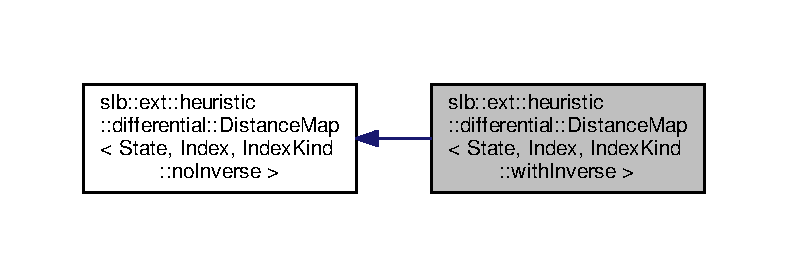
\includegraphics[width=350pt]{structslb_1_1ext_1_1heuristic_1_1differential_1_1DistanceMap_3_01State_00_01Index_00_01IndexKinda4e094b5d26922a6f2ab4a0ee02fc340}
\end{center}
\end{figure}


Collaboration diagram for slb\+:\+:ext\+:\+:heuristic\+:\+:differential\+:\+:Distance\+Map$<$ State, Index, Index\+Kind\+:\+:with\+Inverse $>$\+:\nopagebreak
\begin{figure}[H]
\begin{center}
\leavevmode
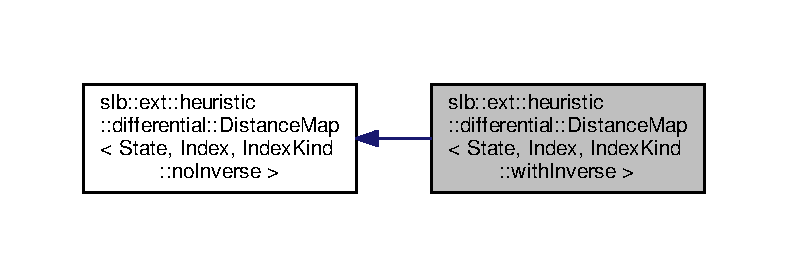
\includegraphics[width=350pt]{structslb_1_1ext_1_1heuristic_1_1differential_1_1DistanceMap_3_01State_00_01Index_00_01IndexKind5190206f8b9116d6815acfc32d1d666f}
\end{center}
\end{figure}
\subsubsection*{Public Types}
\begin{DoxyCompactItemize}
\item 
using \hyperlink{structslb_1_1ext_1_1heuristic_1_1differential_1_1DistanceMap_3_01State_00_01Index_00_01IndexKind_1_1withInverse_01_4_aa8319cee567d1c06cbb753eaa44c73c7}{Base} = \hyperlink{structslb_1_1ext_1_1heuristic_1_1differential_1_1DistanceMap}{Distance\+Map}$<$ State, Index, Index\+Kind\+::no\+Inverse $>$\hypertarget{structslb_1_1ext_1_1heuristic_1_1differential_1_1DistanceMap_3_01State_00_01Index_00_01IndexKind_1_1withInverse_01_4_aa8319cee567d1c06cbb753eaa44c73c7}{}\label{structslb_1_1ext_1_1heuristic_1_1differential_1_1DistanceMap_3_01State_00_01Index_00_01IndexKind_1_1withInverse_01_4_aa8319cee567d1c06cbb753eaa44c73c7}

\begin{DoxyCompactList}\small\item\em The direct base type. \end{DoxyCompactList}\item 
using \hyperlink{structslb_1_1ext_1_1heuristic_1_1differential_1_1DistanceMap_3_01State_00_01Index_00_01IndexKind_1_1withInverse_01_4_ac211f9018ccbc33942eab603d51bace7}{Cost\+Type} = typename \hyperlink{structslb_1_1ext_1_1heuristic_1_1differential_1_1DistanceMap_3_01State_00_01Index_00_01IndexKind_1_1noInverse_01_4_a9a67ddc91fe4ea5fbf6957d2105ed5a7}{Base\+::\+Cost\+Type}\hypertarget{structslb_1_1ext_1_1heuristic_1_1differential_1_1DistanceMap_3_01State_00_01Index_00_01IndexKind_1_1withInverse_01_4_ac211f9018ccbc33942eab603d51bace7}{}\label{structslb_1_1ext_1_1heuristic_1_1differential_1_1DistanceMap_3_01State_00_01Index_00_01IndexKind_1_1withInverse_01_4_ac211f9018ccbc33942eab603d51bace7}

\begin{DoxyCompactList}\small\item\em The action cost type. \end{DoxyCompactList}\item 
using \hyperlink{structslb_1_1ext_1_1heuristic_1_1differential_1_1DistanceMap_3_01State_00_01Index_00_01IndexKind_1_1withInverse_01_4_a8e74432aa27365ae22e8773b5ebda8d2}{Distances} = typename \hyperlink{structslb_1_1ext_1_1heuristic_1_1differential_1_1DistanceMap_3_01State_00_01Index_00_01IndexKind_1_1noInverse_01_4_acba898005faced74c6e3bf42c398f3d8}{Base\+::\+Distances}\hypertarget{structslb_1_1ext_1_1heuristic_1_1differential_1_1DistanceMap_3_01State_00_01Index_00_01IndexKind_1_1withInverse_01_4_a8e74432aa27365ae22e8773b5ebda8d2}{}\label{structslb_1_1ext_1_1heuristic_1_1differential_1_1DistanceMap_3_01State_00_01Index_00_01IndexKind_1_1withInverse_01_4_a8e74432aa27365ae22e8773b5ebda8d2}

\begin{DoxyCompactList}\small\item\em The underlying type for storing distances to pivots. \end{DoxyCompactList}\item 
using \hyperlink{structslb_1_1ext_1_1heuristic_1_1differential_1_1DistanceMap_3_01State_00_01Index_00_01IndexKind_1_1withInverse_01_4_a35bf95bb4cb402c465bc2512c360efc3}{Iterator} = \hyperlink{namespaceslb_1_1core_1_1util_a52016fe00a4fae8791643b870848a79f}{core\+::util\+::\+Vector\+Skip\+Iterator}$<$ \hyperlink{structslb_1_1ext_1_1heuristic_1_1differential_1_1DistanceMap_3_01State_00_01Index_00_01IndexKind_1_1noInverse_01_4_acba898005faced74c6e3bf42c398f3d8}{Distances} $>$\hypertarget{structslb_1_1ext_1_1heuristic_1_1differential_1_1DistanceMap_3_01State_00_01Index_00_01IndexKind_1_1withInverse_01_4_a35bf95bb4cb402c465bc2512c360efc3}{}\label{structslb_1_1ext_1_1heuristic_1_1differential_1_1DistanceMap_3_01State_00_01Index_00_01IndexKind_1_1withInverse_01_4_a35bf95bb4cb402c465bc2512c360efc3}

\begin{DoxyCompactList}\small\item\em The iterator for the distances. \end{DoxyCompactList}\item 
using \hyperlink{structslb_1_1ext_1_1heuristic_1_1differential_1_1DistanceMap_3_01State_00_01Index_00_01IndexKind_1_1withInverse_01_4_ac2abc8b528a584f7a26b7e31fec60f7a}{Const\+Iterator} = \hyperlink{namespaceslb_1_1core_1_1util_a5692b540118495a35ebae95fb8b80790}{core\+::util\+::\+Vector\+Skip\+Const\+Iterator}$<$ \hyperlink{structslb_1_1ext_1_1heuristic_1_1differential_1_1DistanceMap_3_01State_00_01Index_00_01IndexKind_1_1noInverse_01_4_acba898005faced74c6e3bf42c398f3d8}{Distances} $>$\hypertarget{structslb_1_1ext_1_1heuristic_1_1differential_1_1DistanceMap_3_01State_00_01Index_00_01IndexKind_1_1withInverse_01_4_ac2abc8b528a584f7a26b7e31fec60f7a}{}\label{structslb_1_1ext_1_1heuristic_1_1differential_1_1DistanceMap_3_01State_00_01Index_00_01IndexKind_1_1withInverse_01_4_ac2abc8b528a584f7a26b7e31fec60f7a}

\begin{DoxyCompactList}\small\item\em The constant iterator for the distances. \end{DoxyCompactList}\end{DoxyCompactItemize}
\subsubsection*{Public Member Functions}
\begin{DoxyCompactItemize}
\item 
\hyperlink{structslb_1_1ext_1_1heuristic_1_1differential_1_1DistanceMap_3_01State_00_01Index_00_01IndexKind_1_1withInverse_01_4_a35bf95bb4cb402c465bc2512c360efc3}{Iterator} \hyperlink{structslb_1_1ext_1_1heuristic_1_1differential_1_1DistanceMap_3_01State_00_01Index_00_01IndexKind_1_1withInverse_01_4_a74e76bf197c77a72949e7fa837f0ab89}{begin} ()
\begin{DoxyCompactList}\small\item\em Returns iterator to the beginning of the distances. \end{DoxyCompactList}\item 
\hyperlink{structslb_1_1ext_1_1heuristic_1_1differential_1_1DistanceMap_3_01State_00_01Index_00_01IndexKind_1_1withInverse_01_4_ac2abc8b528a584f7a26b7e31fec60f7a}{Const\+Iterator} \hyperlink{structslb_1_1ext_1_1heuristic_1_1differential_1_1DistanceMap_3_01State_00_01Index_00_01IndexKind_1_1withInverse_01_4_a6097346ad9934b5dd878ae49b152e743}{begin} () const 
\begin{DoxyCompactList}\small\item\em Returns constant iterator to the beginning of the distances. \end{DoxyCompactList}\item 
\hyperlink{structslb_1_1ext_1_1heuristic_1_1differential_1_1DistanceMap_3_01State_00_01Index_00_01IndexKind_1_1withInverse_01_4_a35bf95bb4cb402c465bc2512c360efc3}{Iterator} \hyperlink{structslb_1_1ext_1_1heuristic_1_1differential_1_1DistanceMap_3_01State_00_01Index_00_01IndexKind_1_1withInverse_01_4_aa0f1ad0419b0ac53ce9a98c35c53d188}{end} ()
\begin{DoxyCompactList}\small\item\em Returns iterator to the end of the distances. \end{DoxyCompactList}\item 
\hyperlink{structslb_1_1ext_1_1heuristic_1_1differential_1_1DistanceMap_3_01State_00_01Index_00_01IndexKind_1_1withInverse_01_4_ac2abc8b528a584f7a26b7e31fec60f7a}{Const\+Iterator} \hyperlink{structslb_1_1ext_1_1heuristic_1_1differential_1_1DistanceMap_3_01State_00_01Index_00_01IndexKind_1_1withInverse_01_4_a3cf9aef634a0a1c7a78e9fd9ccf326e8}{end} () const 
\begin{DoxyCompactList}\small\item\em Returns constant iterator to the end of the distances. \end{DoxyCompactList}\item 
{\footnotesize template$<$class It $>$ }\\State \hyperlink{structslb_1_1ext_1_1heuristic_1_1differential_1_1DistanceMap_3_01State_00_01Index_00_01IndexKind_1_1withInverse_01_4_a9e5c7a32a51e2e3dcab50c8215d2b8f8}{it\+To\+State} (It it) const 
\begin{DoxyCompactList}\small\item\em Returns the state (from which a distance is stored) corresponding to the given iterator. \end{DoxyCompactList}\item 
{\footnotesize template$<$class Distances1 $>$ }\\void \hyperlink{structslb_1_1ext_1_1heuristic_1_1differential_1_1DistanceMap_3_01State_00_01Index_00_01IndexKind_1_1withInverse_01_4_a098b550f0adfc698960fba13a9593cfe}{intersect} (const Distances1 \&d)
\begin{DoxyCompactList}\small\item\em Computes the minimum of each stored distance and the corresponding distance given by the argument. \end{DoxyCompactList}\item 
State \hyperlink{structslb_1_1ext_1_1heuristic_1_1differential_1_1DistanceMap_3_01State_00_01Index_00_01IndexKind_1_1withInverse_01_4_ae0612ad599cacab6742a174f783f4363}{farthest} () const 
\begin{DoxyCompactList}\small\item\em Returns the state from which the distance is maximal. \end{DoxyCompactList}\end{DoxyCompactItemize}
\subsubsection*{Additional Inherited Members}


\subsubsection{Detailed Description}
\subsubsection*{template$<$class State, class Index$>$\\*
struct slb\+::ext\+::heuristic\+::differential\+::\+Distance\+Map$<$ State, Index, Index\+Kind\+::with\+Inverse $>$}

The type for storing distances to pivots. This specialization is for the case of an index function with an inverse. 


\begin{DoxyTemplParams}{Template Parameters}
{\em State} & The state type representing the search domain. \\
\hline
{\em Index} & Mapping of states to indices. \\
\hline
{\em Index\+Kind} & The type denoting the kind of index. \\
\hline
\end{DoxyTemplParams}


Definition at line 75 of file distance\+\_\+map.\+h.



\subsubsection{Member Function Documentation}
\index{slb\+::ext\+::heuristic\+::differential\+::\+Distance\+Map$<$ State, Index, Index\+Kind\+::with\+Inverse $>$@{slb\+::ext\+::heuristic\+::differential\+::\+Distance\+Map$<$ State, Index, Index\+Kind\+::with\+Inverse $>$}!begin@{begin}}
\index{begin@{begin}!slb\+::ext\+::heuristic\+::differential\+::\+Distance\+Map$<$ State, Index, Index\+Kind\+::with\+Inverse $>$@{slb\+::ext\+::heuristic\+::differential\+::\+Distance\+Map$<$ State, Index, Index\+Kind\+::with\+Inverse $>$}}
\paragraph[{\texorpdfstring{begin()}{begin()}}]{\setlength{\rightskip}{0pt plus 5cm}template$<$class State , class Index $>$ {\bf Iterator} {\bf slb\+::ext\+::heuristic\+::differential\+::\+Distance\+Map}$<$ State, Index, Index\+Kind\+::with\+Inverse $>$\+::begin (
\begin{DoxyParamCaption}
{}
\end{DoxyParamCaption}
)\hspace{0.3cm}{\ttfamily [inline]}}\hypertarget{structslb_1_1ext_1_1heuristic_1_1differential_1_1DistanceMap_3_01State_00_01Index_00_01IndexKind_1_1withInverse_01_4_a74e76bf197c77a72949e7fa837f0ab89}{}\label{structslb_1_1ext_1_1heuristic_1_1differential_1_1DistanceMap_3_01State_00_01Index_00_01IndexKind_1_1withInverse_01_4_a74e76bf197c77a72949e7fa837f0ab89}


Returns iterator to the beginning of the distances. 

\begin{DoxyReturn}{Returns}
Iterator to the beginning of the distances. 
\end{DoxyReturn}


Definition at line 97 of file distance\+\_\+map.\+h.

\index{slb\+::ext\+::heuristic\+::differential\+::\+Distance\+Map$<$ State, Index, Index\+Kind\+::with\+Inverse $>$@{slb\+::ext\+::heuristic\+::differential\+::\+Distance\+Map$<$ State, Index, Index\+Kind\+::with\+Inverse $>$}!begin@{begin}}
\index{begin@{begin}!slb\+::ext\+::heuristic\+::differential\+::\+Distance\+Map$<$ State, Index, Index\+Kind\+::with\+Inverse $>$@{slb\+::ext\+::heuristic\+::differential\+::\+Distance\+Map$<$ State, Index, Index\+Kind\+::with\+Inverse $>$}}
\paragraph[{\texorpdfstring{begin() const }{begin() const }}]{\setlength{\rightskip}{0pt plus 5cm}template$<$class State , class Index $>$ {\bf Const\+Iterator} {\bf slb\+::ext\+::heuristic\+::differential\+::\+Distance\+Map}$<$ State, Index, Index\+Kind\+::with\+Inverse $>$\+::begin (
\begin{DoxyParamCaption}
{}
\end{DoxyParamCaption}
) const\hspace{0.3cm}{\ttfamily [inline]}}\hypertarget{structslb_1_1ext_1_1heuristic_1_1differential_1_1DistanceMap_3_01State_00_01Index_00_01IndexKind_1_1withInverse_01_4_a6097346ad9934b5dd878ae49b152e743}{}\label{structslb_1_1ext_1_1heuristic_1_1differential_1_1DistanceMap_3_01State_00_01Index_00_01IndexKind_1_1withInverse_01_4_a6097346ad9934b5dd878ae49b152e743}


Returns constant iterator to the beginning of the distances. 

\begin{DoxyReturn}{Returns}
Constant iterator to the beginning of the distances. 
\end{DoxyReturn}


Definition at line 103 of file distance\+\_\+map.\+h.

\index{slb\+::ext\+::heuristic\+::differential\+::\+Distance\+Map$<$ State, Index, Index\+Kind\+::with\+Inverse $>$@{slb\+::ext\+::heuristic\+::differential\+::\+Distance\+Map$<$ State, Index, Index\+Kind\+::with\+Inverse $>$}!end@{end}}
\index{end@{end}!slb\+::ext\+::heuristic\+::differential\+::\+Distance\+Map$<$ State, Index, Index\+Kind\+::with\+Inverse $>$@{slb\+::ext\+::heuristic\+::differential\+::\+Distance\+Map$<$ State, Index, Index\+Kind\+::with\+Inverse $>$}}
\paragraph[{\texorpdfstring{end()}{end()}}]{\setlength{\rightskip}{0pt plus 5cm}template$<$class State , class Index $>$ {\bf Iterator} {\bf slb\+::ext\+::heuristic\+::differential\+::\+Distance\+Map}$<$ State, Index, Index\+Kind\+::with\+Inverse $>$\+::end (
\begin{DoxyParamCaption}
{}
\end{DoxyParamCaption}
)\hspace{0.3cm}{\ttfamily [inline]}}\hypertarget{structslb_1_1ext_1_1heuristic_1_1differential_1_1DistanceMap_3_01State_00_01Index_00_01IndexKind_1_1withInverse_01_4_aa0f1ad0419b0ac53ce9a98c35c53d188}{}\label{structslb_1_1ext_1_1heuristic_1_1differential_1_1DistanceMap_3_01State_00_01Index_00_01IndexKind_1_1withInverse_01_4_aa0f1ad0419b0ac53ce9a98c35c53d188}


Returns iterator to the end of the distances. 

\begin{DoxyReturn}{Returns}
Iterator to the end of the distances. 
\end{DoxyReturn}


Definition at line 109 of file distance\+\_\+map.\+h.

\index{slb\+::ext\+::heuristic\+::differential\+::\+Distance\+Map$<$ State, Index, Index\+Kind\+::with\+Inverse $>$@{slb\+::ext\+::heuristic\+::differential\+::\+Distance\+Map$<$ State, Index, Index\+Kind\+::with\+Inverse $>$}!end@{end}}
\index{end@{end}!slb\+::ext\+::heuristic\+::differential\+::\+Distance\+Map$<$ State, Index, Index\+Kind\+::with\+Inverse $>$@{slb\+::ext\+::heuristic\+::differential\+::\+Distance\+Map$<$ State, Index, Index\+Kind\+::with\+Inverse $>$}}
\paragraph[{\texorpdfstring{end() const }{end() const }}]{\setlength{\rightskip}{0pt plus 5cm}template$<$class State , class Index $>$ {\bf Const\+Iterator} {\bf slb\+::ext\+::heuristic\+::differential\+::\+Distance\+Map}$<$ State, Index, Index\+Kind\+::with\+Inverse $>$\+::end (
\begin{DoxyParamCaption}
{}
\end{DoxyParamCaption}
) const\hspace{0.3cm}{\ttfamily [inline]}}\hypertarget{structslb_1_1ext_1_1heuristic_1_1differential_1_1DistanceMap_3_01State_00_01Index_00_01IndexKind_1_1withInverse_01_4_a3cf9aef634a0a1c7a78e9fd9ccf326e8}{}\label{structslb_1_1ext_1_1heuristic_1_1differential_1_1DistanceMap_3_01State_00_01Index_00_01IndexKind_1_1withInverse_01_4_a3cf9aef634a0a1c7a78e9fd9ccf326e8}


Returns constant iterator to the end of the distances. 

\begin{DoxyReturn}{Returns}
Constant iterator to the end of the distances. 
\end{DoxyReturn}


Definition at line 115 of file distance\+\_\+map.\+h.

\index{slb\+::ext\+::heuristic\+::differential\+::\+Distance\+Map$<$ State, Index, Index\+Kind\+::with\+Inverse $>$@{slb\+::ext\+::heuristic\+::differential\+::\+Distance\+Map$<$ State, Index, Index\+Kind\+::with\+Inverse $>$}!farthest@{farthest}}
\index{farthest@{farthest}!slb\+::ext\+::heuristic\+::differential\+::\+Distance\+Map$<$ State, Index, Index\+Kind\+::with\+Inverse $>$@{slb\+::ext\+::heuristic\+::differential\+::\+Distance\+Map$<$ State, Index, Index\+Kind\+::with\+Inverse $>$}}
\paragraph[{\texorpdfstring{farthest() const }{farthest() const }}]{\setlength{\rightskip}{0pt plus 5cm}template$<$class State , class Index $>$ State {\bf slb\+::ext\+::heuristic\+::differential\+::\+Distance\+Map}$<$ State, Index, Index\+Kind\+::with\+Inverse $>$\+::farthest (
\begin{DoxyParamCaption}
{}
\end{DoxyParamCaption}
) const\hspace{0.3cm}{\ttfamily [inline]}}\hypertarget{structslb_1_1ext_1_1heuristic_1_1differential_1_1DistanceMap_3_01State_00_01Index_00_01IndexKind_1_1withInverse_01_4_ae0612ad599cacab6742a174f783f4363}{}\label{structslb_1_1ext_1_1heuristic_1_1differential_1_1DistanceMap_3_01State_00_01Index_00_01IndexKind_1_1withInverse_01_4_ae0612ad599cacab6742a174f783f4363}


Returns the state from which the distance is maximal. 

\begin{DoxyReturn}{Returns}
The state from which the distance is maximal. 
\end{DoxyReturn}


Definition at line 142 of file distance\+\_\+map.\+h.

\index{slb\+::ext\+::heuristic\+::differential\+::\+Distance\+Map$<$ State, Index, Index\+Kind\+::with\+Inverse $>$@{slb\+::ext\+::heuristic\+::differential\+::\+Distance\+Map$<$ State, Index, Index\+Kind\+::with\+Inverse $>$}!intersect@{intersect}}
\index{intersect@{intersect}!slb\+::ext\+::heuristic\+::differential\+::\+Distance\+Map$<$ State, Index, Index\+Kind\+::with\+Inverse $>$@{slb\+::ext\+::heuristic\+::differential\+::\+Distance\+Map$<$ State, Index, Index\+Kind\+::with\+Inverse $>$}}
\paragraph[{\texorpdfstring{intersect(const Distances1 \&d)}{intersect(const Distances1 &d)}}]{\setlength{\rightskip}{0pt plus 5cm}template$<$class State , class Index $>$ template$<$class Distances1 $>$ void {\bf slb\+::ext\+::heuristic\+::differential\+::\+Distance\+Map}$<$ State, Index, Index\+Kind\+::with\+Inverse $>$\+::intersect (
\begin{DoxyParamCaption}
\item[{const Distances1 \&}]{d}
\end{DoxyParamCaption}
)\hspace{0.3cm}{\ttfamily [inline]}}\hypertarget{structslb_1_1ext_1_1heuristic_1_1differential_1_1DistanceMap_3_01State_00_01Index_00_01IndexKind_1_1withInverse_01_4_a098b550f0adfc698960fba13a9593cfe}{}\label{structslb_1_1ext_1_1heuristic_1_1differential_1_1DistanceMap_3_01State_00_01Index_00_01IndexKind_1_1withInverse_01_4_a098b550f0adfc698960fba13a9593cfe}


Computes the minimum of each stored distance and the corresponding distance given by the argument. 


\begin{DoxyTemplParams}{Template Parameters}
{\em Distances1} & The type for the distances given by the argument. \\
\hline
\end{DoxyTemplParams}

\begin{DoxyParams}{Parameters}
{\em d} & The given distances. \\
\hline
\end{DoxyParams}


Definition at line 133 of file distance\+\_\+map.\+h.

\index{slb\+::ext\+::heuristic\+::differential\+::\+Distance\+Map$<$ State, Index, Index\+Kind\+::with\+Inverse $>$@{slb\+::ext\+::heuristic\+::differential\+::\+Distance\+Map$<$ State, Index, Index\+Kind\+::with\+Inverse $>$}!it\+To\+State@{it\+To\+State}}
\index{it\+To\+State@{it\+To\+State}!slb\+::ext\+::heuristic\+::differential\+::\+Distance\+Map$<$ State, Index, Index\+Kind\+::with\+Inverse $>$@{slb\+::ext\+::heuristic\+::differential\+::\+Distance\+Map$<$ State, Index, Index\+Kind\+::with\+Inverse $>$}}
\paragraph[{\texorpdfstring{it\+To\+State(\+It it) const }{itToState(It it) const }}]{\setlength{\rightskip}{0pt plus 5cm}template$<$class State , class Index $>$ template$<$class It $>$ State {\bf slb\+::ext\+::heuristic\+::differential\+::\+Distance\+Map}$<$ State, Index, Index\+Kind\+::with\+Inverse $>$\+::it\+To\+State (
\begin{DoxyParamCaption}
\item[{It}]{it}
\end{DoxyParamCaption}
) const\hspace{0.3cm}{\ttfamily [inline]}}\hypertarget{structslb_1_1ext_1_1heuristic_1_1differential_1_1DistanceMap_3_01State_00_01Index_00_01IndexKind_1_1withInverse_01_4_a9e5c7a32a51e2e3dcab50c8215d2b8f8}{}\label{structslb_1_1ext_1_1heuristic_1_1differential_1_1DistanceMap_3_01State_00_01Index_00_01IndexKind_1_1withInverse_01_4_a9e5c7a32a51e2e3dcab50c8215d2b8f8}


Returns the state (from which a distance is stored) corresponding to the given iterator. 


\begin{DoxyTemplParams}{Template Parameters}
{\em It} & The iterator type. \\
\hline
\end{DoxyTemplParams}

\begin{DoxyParams}{Parameters}
{\em it} & The given iterator. \\
\hline
\end{DoxyParams}
\begin{DoxyReturn}{Returns}
the state (from which a distance is stored) corresponding to {\ttfamily it} 
\end{DoxyReturn}


Definition at line 126 of file distance\+\_\+map.\+h.



The documentation for this struct was generated from the following file\+:\begin{DoxyCompactItemize}
\item 
extensions/heuristics/differential/\hyperlink{distance__map_8h}{distance\+\_\+map.\+h}\end{DoxyCompactItemize}

\hypertarget{structslb_1_1ext_1_1heuristic_1_1differential_1_1DistancesToPivots}{}\subsection{slb\+:\+:ext\+:\+:heuristic\+:\+:differential\+:\+:Distances\+To\+Pivots$<$ State, Index, k $>$ Struct Template Reference}
\label{structslb_1_1ext_1_1heuristic_1_1differential_1_1DistancesToPivots}\index{slb\+::ext\+::heuristic\+::differential\+::\+Distances\+To\+Pivots$<$ State, Index, k $>$@{slb\+::ext\+::heuristic\+::differential\+::\+Distances\+To\+Pivots$<$ State, Index, k $>$}}


The type for working with distances to pivots. The general definition is for the situation with an index. The situation without an index is handled by a specialization.  




{\ttfamily \#include $<$distances\+\_\+to\+\_\+pivots.\+h$>$}

\subsubsection*{Public Types}
\begin{DoxyCompactItemize}
\item 
using \hyperlink{structslb_1_1ext_1_1heuristic_1_1differential_1_1DistancesToPivots_a8b02847b92f84e1d3d97b71c91409e62}{Cost\+Type} = typename State\+::\+Cost\+Type\hypertarget{structslb_1_1ext_1_1heuristic_1_1differential_1_1DistancesToPivots_a8b02847b92f84e1d3d97b71c91409e62}{}\label{structslb_1_1ext_1_1heuristic_1_1differential_1_1DistancesToPivots_a8b02847b92f84e1d3d97b71c91409e62}

\begin{DoxyCompactList}\small\item\em The action cost type. \end{DoxyCompactList}\item 
using \hyperlink{structslb_1_1ext_1_1heuristic_1_1differential_1_1DistancesToPivots_af1bead3d0ade455bbe8901d3adfbd62b}{Distances} = std\+::vector$<$ \hyperlink{structslb_1_1ext_1_1heuristic_1_1differential_1_1DistancesToPivots_a8b02847b92f84e1d3d97b71c91409e62}{Cost\+Type} $>$\hypertarget{structslb_1_1ext_1_1heuristic_1_1differential_1_1DistancesToPivots_af1bead3d0ade455bbe8901d3adfbd62b}{}\label{structslb_1_1ext_1_1heuristic_1_1differential_1_1DistancesToPivots_af1bead3d0ade455bbe8901d3adfbd62b}

\begin{DoxyCompactList}\small\item\em The type for storing distances to pivots. \end{DoxyCompactList}\item 
using \hyperlink{structslb_1_1ext_1_1heuristic_1_1differential_1_1DistancesToPivots_aa307465e8919ae3f3e93f5aa1f6e4b6f}{It} = typename std\+::vector$<$ \hyperlink{structslb_1_1ext_1_1heuristic_1_1differential_1_1DistancesToPivots_a8b02847b92f84e1d3d97b71c91409e62}{Cost\+Type} $>$\+::const\+\_\+iterator\hypertarget{structslb_1_1ext_1_1heuristic_1_1differential_1_1DistancesToPivots_aa307465e8919ae3f3e93f5aa1f6e4b6f}{}\label{structslb_1_1ext_1_1heuristic_1_1differential_1_1DistancesToPivots_aa307465e8919ae3f3e93f5aa1f6e4b6f}

\begin{DoxyCompactList}\small\item\em The iterator for the distances to pivots. \end{DoxyCompactList}\end{DoxyCompactItemize}
\subsubsection*{Public Member Functions}
\begin{DoxyCompactItemize}
\item 
void \hyperlink{structslb_1_1ext_1_1heuristic_1_1differential_1_1DistancesToPivots_a8cf1541be1ef95ec622c2eb4521b3839}{update\+Expected\+N\+Pivots} (int expected\+N\+Pivots)\hypertarget{structslb_1_1ext_1_1heuristic_1_1differential_1_1DistancesToPivots_a8cf1541be1ef95ec622c2eb4521b3839}{}\label{structslb_1_1ext_1_1heuristic_1_1differential_1_1DistancesToPivots_a8cf1541be1ef95ec622c2eb4521b3839}

\begin{DoxyCompactList}\small\item\em Updates the expected number of pivots. \end{DoxyCompactList}\item 
{\footnotesize template$<$class My\+Distance\+Map $>$ }\\void \hyperlink{structslb_1_1ext_1_1heuristic_1_1differential_1_1DistancesToPivots_af7dfc673a6ee47fde2300816ed97c3f3}{append} (const My\+Distance\+Map \&my\+Map)
\begin{DoxyCompactList}\small\item\em Appends the given distances to the existing ones. \end{DoxyCompactList}\item 
\hyperlink{structslb_1_1ext_1_1heuristic_1_1differential_1_1DistancesToPivots_aa307465e8919ae3f3e93f5aa1f6e4b6f}{It} \hyperlink{structslb_1_1ext_1_1heuristic_1_1differential_1_1DistancesToPivots_ac995c37475f0e2ec6444d0f5d7d56dd9}{pivot\+It} (const State \&s) const 
\begin{DoxyCompactList}\small\item\em Returns the iterator to the first distance to pivot from the given state. \end{DoxyCompactList}\item 
int \hyperlink{structslb_1_1ext_1_1heuristic_1_1differential_1_1DistancesToPivots_ae477ef19891e31a53fcf000351f7ad66}{n\+Pivots} () const 
\begin{DoxyCompactList}\small\item\em Returns the number of pivots. \end{DoxyCompactList}\item 
void \hyperlink{structslb_1_1ext_1_1heuristic_1_1differential_1_1DistancesToPivots_a7eda75981b7771532823eb013d9b240e}{clear} ()\hypertarget{structslb_1_1ext_1_1heuristic_1_1differential_1_1DistancesToPivots_a7eda75981b7771532823eb013d9b240e}{}\label{structslb_1_1ext_1_1heuristic_1_1differential_1_1DistancesToPivots_a7eda75981b7771532823eb013d9b240e}

\begin{DoxyCompactList}\small\item\em Clears all the distances. \end{DoxyCompactList}\end{DoxyCompactItemize}
\subsubsection*{Private Attributes}
\begin{DoxyCompactItemize}
\item 
int \hyperlink{structslb_1_1ext_1_1heuristic_1_1differential_1_1DistancesToPivots_a57e0ac0329ae9755dc23d917e14c090a}{expected\+N\+Pivots\+\_\+}\hypertarget{structslb_1_1ext_1_1heuristic_1_1differential_1_1DistancesToPivots_a57e0ac0329ae9755dc23d917e14c090a}{}\label{structslb_1_1ext_1_1heuristic_1_1differential_1_1DistancesToPivots_a57e0ac0329ae9755dc23d917e14c090a}

\begin{DoxyCompactList}\small\item\em The expected number of pivots. \end{DoxyCompactList}\item 
int \hyperlink{structslb_1_1ext_1_1heuristic_1_1differential_1_1DistancesToPivots_a7f7561b20fd174fb2436c3ce1744913e}{n\+Pivots\+\_\+} = 0\hypertarget{structslb_1_1ext_1_1heuristic_1_1differential_1_1DistancesToPivots_a7f7561b20fd174fb2436c3ce1744913e}{}\label{structslb_1_1ext_1_1heuristic_1_1differential_1_1DistancesToPivots_a7f7561b20fd174fb2436c3ce1744913e}

\begin{DoxyCompactList}\small\item\em The number of pivots $<$ to which distances have been added. \end{DoxyCompactList}\item 
\hyperlink{structslb_1_1ext_1_1heuristic_1_1differential_1_1DistancesToPivots_af1bead3d0ade455bbe8901d3adfbd62b}{Distances} \hyperlink{structslb_1_1ext_1_1heuristic_1_1differential_1_1DistancesToPivots_acd953ab649dda7ede08611cda2e2ce62}{distances\+\_\+}\hypertarget{structslb_1_1ext_1_1heuristic_1_1differential_1_1DistancesToPivots_acd953ab649dda7ede08611cda2e2ce62}{}\label{structslb_1_1ext_1_1heuristic_1_1differential_1_1DistancesToPivots_acd953ab649dda7ede08611cda2e2ce62}

\begin{DoxyCompactList}\small\item\em Distances to pivots. \end{DoxyCompactList}\end{DoxyCompactItemize}


\subsubsection{Detailed Description}
\subsubsection*{template$<$class State, class Index = No\+Index, Index\+Kind k = Index\+::kind$>$\\*
struct slb\+::ext\+::heuristic\+::differential\+::\+Distances\+To\+Pivots$<$ State, Index, k $>$}

The type for working with distances to pivots. The general definition is for the situation with an index. The situation without an index is handled by a specialization. 


\begin{DoxyTemplParams}{Template Parameters}
{\em State} & The state type representing the search domain. \\
\hline
{\em Index} & Mapping of states to indices. \\
\hline
{\em Index\+Kind} & The type denoting the kind of index. \\
\hline
\end{DoxyTemplParams}


Definition at line 20 of file distances\+\_\+to\+\_\+pivots.\+h.



\subsubsection{Member Function Documentation}
\index{slb\+::ext\+::heuristic\+::differential\+::\+Distances\+To\+Pivots@{slb\+::ext\+::heuristic\+::differential\+::\+Distances\+To\+Pivots}!append@{append}}
\index{append@{append}!slb\+::ext\+::heuristic\+::differential\+::\+Distances\+To\+Pivots@{slb\+::ext\+::heuristic\+::differential\+::\+Distances\+To\+Pivots}}
\paragraph[{\texorpdfstring{append(const My\+Distance\+Map \&my\+Map)}{append(const MyDistanceMap &myMap)}}]{\setlength{\rightskip}{0pt plus 5cm}template$<$class State , class Index  = No\+Index, Index\+Kind k = Index\+::kind$>$ template$<$class My\+Distance\+Map $>$ void {\bf slb\+::ext\+::heuristic\+::differential\+::\+Distances\+To\+Pivots}$<$ State, Index, k $>$\+::append (
\begin{DoxyParamCaption}
\item[{const My\+Distance\+Map \&}]{my\+Map}
\end{DoxyParamCaption}
)\hspace{0.3cm}{\ttfamily [inline]}}\hypertarget{structslb_1_1ext_1_1heuristic_1_1differential_1_1DistancesToPivots_af7dfc673a6ee47fde2300816ed97c3f3}{}\label{structslb_1_1ext_1_1heuristic_1_1differential_1_1DistancesToPivots_af7dfc673a6ee47fde2300816ed97c3f3}


Appends the given distances to the existing ones. 


\begin{DoxyTemplParams}{Template Parameters}
{\em My\+Distance\+Map} & The type for storing the distances to be appended. \\
\hline
\end{DoxyTemplParams}

\begin{DoxyParams}{Parameters}
{\em my\+Map} & The distances to be appended. \\
\hline
\end{DoxyParams}
\begin{DoxyNote}{Note}
My\+Distance\+Map must provide begin() and end() associated with iterator over states, so it cannot be the \hyperlink{structslb_1_1ext_1_1heuristic_1_1differential_1_1DistanceMap}{Distance\+Map} with index without an inverse. 
\end{DoxyNote}


Definition at line 42 of file distances\+\_\+to\+\_\+pivots.\+h.

\index{slb\+::ext\+::heuristic\+::differential\+::\+Distances\+To\+Pivots@{slb\+::ext\+::heuristic\+::differential\+::\+Distances\+To\+Pivots}!n\+Pivots@{n\+Pivots}}
\index{n\+Pivots@{n\+Pivots}!slb\+::ext\+::heuristic\+::differential\+::\+Distances\+To\+Pivots@{slb\+::ext\+::heuristic\+::differential\+::\+Distances\+To\+Pivots}}
\paragraph[{\texorpdfstring{n\+Pivots() const }{nPivots() const }}]{\setlength{\rightskip}{0pt plus 5cm}template$<$class State , class Index  = No\+Index, Index\+Kind k = Index\+::kind$>$ int {\bf slb\+::ext\+::heuristic\+::differential\+::\+Distances\+To\+Pivots}$<$ State, Index, k $>$\+::n\+Pivots (
\begin{DoxyParamCaption}
{}
\end{DoxyParamCaption}
) const\hspace{0.3cm}{\ttfamily [inline]}}\hypertarget{structslb_1_1ext_1_1heuristic_1_1differential_1_1DistancesToPivots_ae477ef19891e31a53fcf000351f7ad66}{}\label{structslb_1_1ext_1_1heuristic_1_1differential_1_1DistancesToPivots_ae477ef19891e31a53fcf000351f7ad66}


Returns the number of pivots. 

\begin{DoxyReturn}{Returns}
The number of pivots. 
\end{DoxyReturn}


Definition at line 62 of file distances\+\_\+to\+\_\+pivots.\+h.

\index{slb\+::ext\+::heuristic\+::differential\+::\+Distances\+To\+Pivots@{slb\+::ext\+::heuristic\+::differential\+::\+Distances\+To\+Pivots}!pivot\+It@{pivot\+It}}
\index{pivot\+It@{pivot\+It}!slb\+::ext\+::heuristic\+::differential\+::\+Distances\+To\+Pivots@{slb\+::ext\+::heuristic\+::differential\+::\+Distances\+To\+Pivots}}
\paragraph[{\texorpdfstring{pivot\+It(const State \&s) const }{pivotIt(const State &s) const }}]{\setlength{\rightskip}{0pt plus 5cm}template$<$class State , class Index  = No\+Index, Index\+Kind k = Index\+::kind$>$ {\bf It} {\bf slb\+::ext\+::heuristic\+::differential\+::\+Distances\+To\+Pivots}$<$ State, Index, k $>$\+::pivot\+It (
\begin{DoxyParamCaption}
\item[{const State \&}]{s}
\end{DoxyParamCaption}
) const\hspace{0.3cm}{\ttfamily [inline]}}\hypertarget{structslb_1_1ext_1_1heuristic_1_1differential_1_1DistancesToPivots_ac995c37475f0e2ec6444d0f5d7d56dd9}{}\label{structslb_1_1ext_1_1heuristic_1_1differential_1_1DistancesToPivots_ac995c37475f0e2ec6444d0f5d7d56dd9}


Returns the iterator to the first distance to pivot from the given state. 


\begin{DoxyParams}{Parameters}
{\em s} & The given state. \\
\hline
\end{DoxyParams}
\begin{DoxyReturn}{Returns}
The iterator to the first distance to pivot from {\ttfamily s}. 
\end{DoxyReturn}


Definition at line 56 of file distances\+\_\+to\+\_\+pivots.\+h.



The documentation for this struct was generated from the following file\+:\begin{DoxyCompactItemize}
\item 
extensions/heuristics/differential/\hyperlink{distances__to__pivots_8h}{distances\+\_\+to\+\_\+pivots.\+h}\end{DoxyCompactItemize}

\hypertarget{structslb_1_1ext_1_1heuristic_1_1differential_1_1DistancesToPivots_3_01State_00_01Index_00_01IndexKind_1_1none_01_4}{}\subsection{slb\+:\+:ext\+:\+:heuristic\+:\+:differential\+:\+:Distances\+To\+Pivots$<$ State, Index, Index\+Kind\+:\+:none $>$ Struct Template Reference}
\label{structslb_1_1ext_1_1heuristic_1_1differential_1_1DistancesToPivots_3_01State_00_01Index_00_01IndexKind_1_1none_01_4}\index{slb\+::ext\+::heuristic\+::differential\+::\+Distances\+To\+Pivots$<$ State, Index, Index\+Kind\+::none $>$@{slb\+::ext\+::heuristic\+::differential\+::\+Distances\+To\+Pivots$<$ State, Index, Index\+Kind\+::none $>$}}


The type for working with distances to pivots. This specialization is for the situation without an index.  




{\ttfamily \#include $<$distances\+\_\+to\+\_\+pivots.\+h$>$}

\subsubsection*{Public Types}
\begin{DoxyCompactItemize}
\item 
using \hyperlink{structslb_1_1ext_1_1heuristic_1_1differential_1_1DistancesToPivots_3_01State_00_01Index_00_01IndexKind_1_1none_01_4_a49aceeabea79ded5ed2911ae4a41e30b}{Cost\+Type} = typename State\+::\+Cost\+Type\hypertarget{structslb_1_1ext_1_1heuristic_1_1differential_1_1DistancesToPivots_3_01State_00_01Index_00_01IndexKind_1_1none_01_4_a49aceeabea79ded5ed2911ae4a41e30b}{}\label{structslb_1_1ext_1_1heuristic_1_1differential_1_1DistancesToPivots_3_01State_00_01Index_00_01IndexKind_1_1none_01_4_a49aceeabea79ded5ed2911ae4a41e30b}

\begin{DoxyCompactList}\small\item\em The action cost type. \end{DoxyCompactList}\item 
using \hyperlink{structslb_1_1ext_1_1heuristic_1_1differential_1_1DistancesToPivots_3_01State_00_01Index_00_01IndexKind_1_1none_01_4_ad9594df4b94a787fdb75d0ed2617d276}{Distances} = std\+::unordered\+\_\+map$<$ State, std\+::vector$<$ \hyperlink{structslb_1_1ext_1_1heuristic_1_1differential_1_1DistancesToPivots_3_01State_00_01Index_00_01IndexKind_1_1none_01_4_a49aceeabea79ded5ed2911ae4a41e30b}{Cost\+Type} $>$, \hyperlink{structslb_1_1core_1_1util_1_1StateHash}{core\+::util\+::\+State\+Hash}$<$ State $>$$>$\hypertarget{structslb_1_1ext_1_1heuristic_1_1differential_1_1DistancesToPivots_3_01State_00_01Index_00_01IndexKind_1_1none_01_4_ad9594df4b94a787fdb75d0ed2617d276}{}\label{structslb_1_1ext_1_1heuristic_1_1differential_1_1DistancesToPivots_3_01State_00_01Index_00_01IndexKind_1_1none_01_4_ad9594df4b94a787fdb75d0ed2617d276}

\begin{DoxyCompactList}\small\item\em The type for storing distances to pivots. \end{DoxyCompactList}\item 
using \hyperlink{structslb_1_1ext_1_1heuristic_1_1differential_1_1DistancesToPivots_3_01State_00_01Index_00_01IndexKind_1_1none_01_4_a718032b836ed77cb94b3c37389c0d5ed}{It} = typename std\+::vector$<$ \hyperlink{structslb_1_1ext_1_1heuristic_1_1differential_1_1DistancesToPivots_3_01State_00_01Index_00_01IndexKind_1_1none_01_4_a49aceeabea79ded5ed2911ae4a41e30b}{Cost\+Type} $>$\+::const\+\_\+iterator\hypertarget{structslb_1_1ext_1_1heuristic_1_1differential_1_1DistancesToPivots_3_01State_00_01Index_00_01IndexKind_1_1none_01_4_a718032b836ed77cb94b3c37389c0d5ed}{}\label{structslb_1_1ext_1_1heuristic_1_1differential_1_1DistancesToPivots_3_01State_00_01Index_00_01IndexKind_1_1none_01_4_a718032b836ed77cb94b3c37389c0d5ed}

\begin{DoxyCompactList}\small\item\em The iterator for the distances to pivots. \end{DoxyCompactList}\end{DoxyCompactItemize}
\subsubsection*{Public Member Functions}
\begin{DoxyCompactItemize}
\item 
{\footnotesize template$<$class My\+Distance\+Map $>$ }\\void \hyperlink{structslb_1_1ext_1_1heuristic_1_1differential_1_1DistancesToPivots_3_01State_00_01Index_00_01IndexKind_1_1none_01_4_a126e633fa3a611519726896247b33527}{append} (const My\+Distance\+Map \&my\+Map)
\begin{DoxyCompactList}\small\item\em Appends the given distances to the existing ones. \end{DoxyCompactList}\item 
\hyperlink{structslb_1_1ext_1_1heuristic_1_1differential_1_1DistancesToPivots_3_01State_00_01Index_00_01IndexKind_1_1none_01_4_a718032b836ed77cb94b3c37389c0d5ed}{It} \hyperlink{structslb_1_1ext_1_1heuristic_1_1differential_1_1DistancesToPivots_3_01State_00_01Index_00_01IndexKind_1_1none_01_4_ace3b1e082a65142bb9f6f23dea9ed0e1}{pivot\+It} (const State \&s) const 
\begin{DoxyCompactList}\small\item\em Returns the iterator to the first distance to pivot from the given state. \end{DoxyCompactList}\item 
int \hyperlink{structslb_1_1ext_1_1heuristic_1_1differential_1_1DistancesToPivots_3_01State_00_01Index_00_01IndexKind_1_1none_01_4_af8c3961a29a41a2cc9a1d04dfe407f80}{n\+Pivots} () const 
\begin{DoxyCompactList}\small\item\em Returns the number of pivots. \end{DoxyCompactList}\item 
void \hyperlink{structslb_1_1ext_1_1heuristic_1_1differential_1_1DistancesToPivots_3_01State_00_01Index_00_01IndexKind_1_1none_01_4_a4335318626588baa4d08652ec67f1890}{clear} ()\hypertarget{structslb_1_1ext_1_1heuristic_1_1differential_1_1DistancesToPivots_3_01State_00_01Index_00_01IndexKind_1_1none_01_4_a4335318626588baa4d08652ec67f1890}{}\label{structslb_1_1ext_1_1heuristic_1_1differential_1_1DistancesToPivots_3_01State_00_01Index_00_01IndexKind_1_1none_01_4_a4335318626588baa4d08652ec67f1890}

\begin{DoxyCompactList}\small\item\em Clears all the distances. \end{DoxyCompactList}\end{DoxyCompactItemize}
\subsubsection*{Private Attributes}
\begin{DoxyCompactItemize}
\item 
int \hyperlink{structslb_1_1ext_1_1heuristic_1_1differential_1_1DistancesToPivots_3_01State_00_01Index_00_01IndexKind_1_1none_01_4_ada16b37eefe345e3bda862e3550cf997}{n\+Pivots\+\_\+} = 0\hypertarget{structslb_1_1ext_1_1heuristic_1_1differential_1_1DistancesToPivots_3_01State_00_01Index_00_01IndexKind_1_1none_01_4_ada16b37eefe345e3bda862e3550cf997}{}\label{structslb_1_1ext_1_1heuristic_1_1differential_1_1DistancesToPivots_3_01State_00_01Index_00_01IndexKind_1_1none_01_4_ada16b37eefe345e3bda862e3550cf997}

\begin{DoxyCompactList}\small\item\em The number of pivots $<$ to which distances have been added. \end{DoxyCompactList}\item 
\hyperlink{structslb_1_1ext_1_1heuristic_1_1differential_1_1DistancesToPivots_3_01State_00_01Index_00_01IndexKind_1_1none_01_4_ad9594df4b94a787fdb75d0ed2617d276}{Distances} \hyperlink{structslb_1_1ext_1_1heuristic_1_1differential_1_1DistancesToPivots_3_01State_00_01Index_00_01IndexKind_1_1none_01_4_a86393e0db863e02672fd684342538526}{distances\+\_\+}\hypertarget{structslb_1_1ext_1_1heuristic_1_1differential_1_1DistancesToPivots_3_01State_00_01Index_00_01IndexKind_1_1none_01_4_a86393e0db863e02672fd684342538526}{}\label{structslb_1_1ext_1_1heuristic_1_1differential_1_1DistancesToPivots_3_01State_00_01Index_00_01IndexKind_1_1none_01_4_a86393e0db863e02672fd684342538526}

\begin{DoxyCompactList}\small\item\em Distances to pivots. \end{DoxyCompactList}\end{DoxyCompactItemize}


\subsubsection{Detailed Description}
\subsubsection*{template$<$class State, class Index$>$\\*
struct slb\+::ext\+::heuristic\+::differential\+::\+Distances\+To\+Pivots$<$ State, Index, Index\+Kind\+::none $>$}

The type for working with distances to pivots. This specialization is for the situation without an index. 


\begin{DoxyTemplParams}{Template Parameters}
{\em State} & The state type representing the search domain. \\
\hline
{\em Index} & Mapping of states to indices. \\
\hline
{\em Index\+Kind} & The type denoting the kind of index. \\
\hline
\end{DoxyTemplParams}


Definition at line 83 of file distances\+\_\+to\+\_\+pivots.\+h.



\subsubsection{Member Function Documentation}
\index{slb\+::ext\+::heuristic\+::differential\+::\+Distances\+To\+Pivots$<$ State, Index, Index\+Kind\+::none $>$@{slb\+::ext\+::heuristic\+::differential\+::\+Distances\+To\+Pivots$<$ State, Index, Index\+Kind\+::none $>$}!append@{append}}
\index{append@{append}!slb\+::ext\+::heuristic\+::differential\+::\+Distances\+To\+Pivots$<$ State, Index, Index\+Kind\+::none $>$@{slb\+::ext\+::heuristic\+::differential\+::\+Distances\+To\+Pivots$<$ State, Index, Index\+Kind\+::none $>$}}
\paragraph[{\texorpdfstring{append(const My\+Distance\+Map \&my\+Map)}{append(const MyDistanceMap &myMap)}}]{\setlength{\rightskip}{0pt plus 5cm}template$<$class State , class Index $>$ template$<$class My\+Distance\+Map $>$ void {\bf slb\+::ext\+::heuristic\+::differential\+::\+Distances\+To\+Pivots}$<$ State, Index, Index\+Kind\+::none $>$\+::append (
\begin{DoxyParamCaption}
\item[{const My\+Distance\+Map \&}]{my\+Map}
\end{DoxyParamCaption}
)\hspace{0.3cm}{\ttfamily [inline]}}\hypertarget{structslb_1_1ext_1_1heuristic_1_1differential_1_1DistancesToPivots_3_01State_00_01Index_00_01IndexKind_1_1none_01_4_a126e633fa3a611519726896247b33527}{}\label{structslb_1_1ext_1_1heuristic_1_1differential_1_1DistancesToPivots_3_01State_00_01Index_00_01IndexKind_1_1none_01_4_a126e633fa3a611519726896247b33527}


Appends the given distances to the existing ones. 


\begin{DoxyTemplParams}{Template Parameters}
{\em My\+Distance\+Map} & The type for storing the distances to be appended. \\
\hline
\end{DoxyTemplParams}

\begin{DoxyParams}{Parameters}
{\em my\+Map} & The distances to be appended. \\
\hline
\end{DoxyParams}
\begin{DoxyNote}{Note}
My\+Distance\+Map must provide begin() and end() associated with iterator over states, so it cannot be the \hyperlink{structslb_1_1ext_1_1heuristic_1_1differential_1_1DistanceMap}{Distance\+Map} with index without an inverse. 
\end{DoxyNote}


Definition at line 101 of file distances\+\_\+to\+\_\+pivots.\+h.

\index{slb\+::ext\+::heuristic\+::differential\+::\+Distances\+To\+Pivots$<$ State, Index, Index\+Kind\+::none $>$@{slb\+::ext\+::heuristic\+::differential\+::\+Distances\+To\+Pivots$<$ State, Index, Index\+Kind\+::none $>$}!n\+Pivots@{n\+Pivots}}
\index{n\+Pivots@{n\+Pivots}!slb\+::ext\+::heuristic\+::differential\+::\+Distances\+To\+Pivots$<$ State, Index, Index\+Kind\+::none $>$@{slb\+::ext\+::heuristic\+::differential\+::\+Distances\+To\+Pivots$<$ State, Index, Index\+Kind\+::none $>$}}
\paragraph[{\texorpdfstring{n\+Pivots() const }{nPivots() const }}]{\setlength{\rightskip}{0pt plus 5cm}template$<$class State , class Index $>$ int {\bf slb\+::ext\+::heuristic\+::differential\+::\+Distances\+To\+Pivots}$<$ State, Index, Index\+Kind\+::none $>$\+::n\+Pivots (
\begin{DoxyParamCaption}
{}
\end{DoxyParamCaption}
) const\hspace{0.3cm}{\ttfamily [inline]}}\hypertarget{structslb_1_1ext_1_1heuristic_1_1differential_1_1DistancesToPivots_3_01State_00_01Index_00_01IndexKind_1_1none_01_4_af8c3961a29a41a2cc9a1d04dfe407f80}{}\label{structslb_1_1ext_1_1heuristic_1_1differential_1_1DistancesToPivots_3_01State_00_01Index_00_01IndexKind_1_1none_01_4_af8c3961a29a41a2cc9a1d04dfe407f80}


Returns the number of pivots. 

\begin{DoxyReturn}{Returns}
The number of pivots. 
\end{DoxyReturn}


Definition at line 119 of file distances\+\_\+to\+\_\+pivots.\+h.

\index{slb\+::ext\+::heuristic\+::differential\+::\+Distances\+To\+Pivots$<$ State, Index, Index\+Kind\+::none $>$@{slb\+::ext\+::heuristic\+::differential\+::\+Distances\+To\+Pivots$<$ State, Index, Index\+Kind\+::none $>$}!pivot\+It@{pivot\+It}}
\index{pivot\+It@{pivot\+It}!slb\+::ext\+::heuristic\+::differential\+::\+Distances\+To\+Pivots$<$ State, Index, Index\+Kind\+::none $>$@{slb\+::ext\+::heuristic\+::differential\+::\+Distances\+To\+Pivots$<$ State, Index, Index\+Kind\+::none $>$}}
\paragraph[{\texorpdfstring{pivot\+It(const State \&s) const }{pivotIt(const State &s) const }}]{\setlength{\rightskip}{0pt plus 5cm}template$<$class State , class Index $>$ {\bf It} {\bf slb\+::ext\+::heuristic\+::differential\+::\+Distances\+To\+Pivots}$<$ State, Index, Index\+Kind\+::none $>$\+::pivot\+It (
\begin{DoxyParamCaption}
\item[{const State \&}]{s}
\end{DoxyParamCaption}
) const\hspace{0.3cm}{\ttfamily [inline]}}\hypertarget{structslb_1_1ext_1_1heuristic_1_1differential_1_1DistancesToPivots_3_01State_00_01Index_00_01IndexKind_1_1none_01_4_ace3b1e082a65142bb9f6f23dea9ed0e1}{}\label{structslb_1_1ext_1_1heuristic_1_1differential_1_1DistancesToPivots_3_01State_00_01Index_00_01IndexKind_1_1none_01_4_ace3b1e082a65142bb9f6f23dea9ed0e1}


Returns the iterator to the first distance to pivot from the given state. 


\begin{DoxyParams}{Parameters}
{\em s} & The given state. \\
\hline
\end{DoxyParams}
\begin{DoxyReturn}{Returns}
The iterator to the first distance to pivot from {\ttfamily s}. 
\end{DoxyReturn}


Definition at line 111 of file distances\+\_\+to\+\_\+pivots.\+h.



The documentation for this struct was generated from the following file\+:\begin{DoxyCompactItemize}
\item 
extensions/heuristics/differential/\hyperlink{distances__to__pivots_8h}{distances\+\_\+to\+\_\+pivots.\+h}\end{DoxyCompactItemize}

\hypertarget{structslb_1_1core_1_1sb_1_1DomainBase}{}\subsection{slb\+:\+:core\+:\+:sb\+:\+:Domain\+Base Struct Reference}
\label{structslb_1_1core_1_1sb_1_1DomainBase}\index{slb\+::core\+::sb\+::\+Domain\+Base@{slb\+::core\+::sb\+::\+Domain\+Base}}


A type for common features of domains.  




{\ttfamily \#include $<$domain\+\_\+base.\+h$>$}



Inheritance diagram for slb\+:\+:core\+:\+:sb\+:\+:Domain\+Base\+:\nopagebreak
\begin{figure}[H]
\begin{center}
\leavevmode
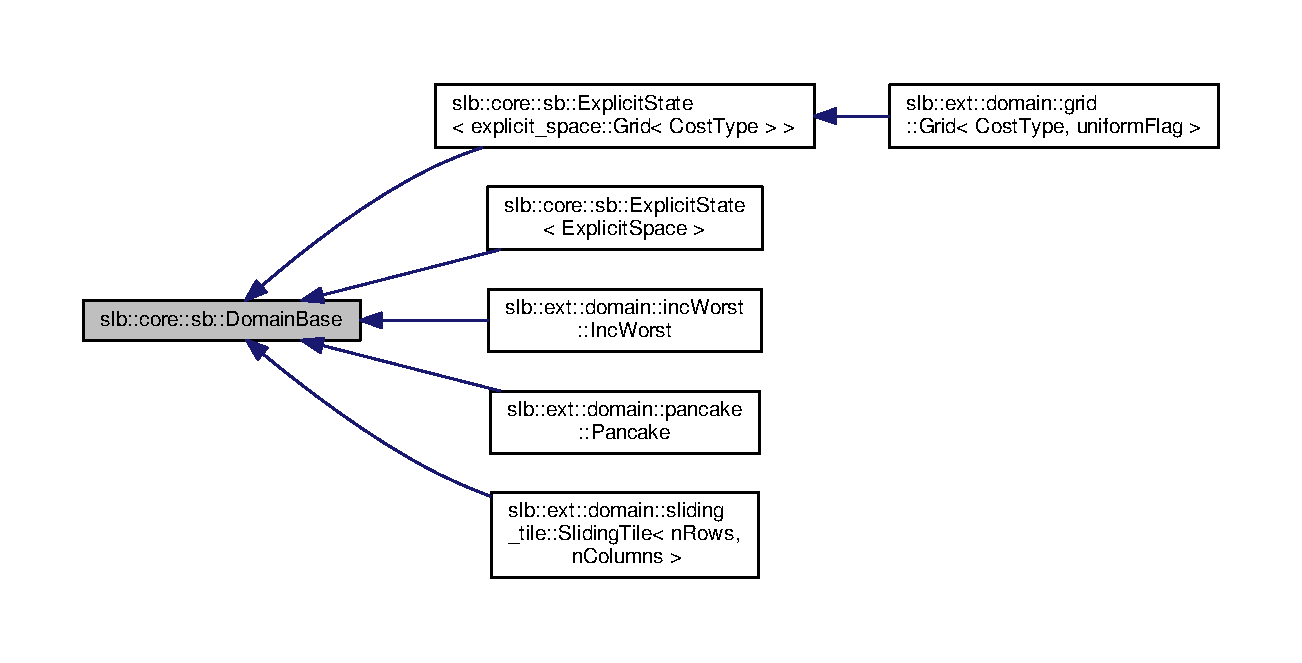
\includegraphics[width=350pt]{structslb_1_1core_1_1sb_1_1DomainBase__inherit__graph}
\end{center}
\end{figure}
\subsubsection*{Public Member Functions}
\begin{DoxyCompactItemize}
\item 
std\+::string \hyperlink{structslb_1_1core_1_1sb_1_1DomainBase_a854e1cc1b1eec278542c200e19f48aef}{visual\+Label} () const 
\begin{DoxyCompactList}\small\item\em Returns the textual label for the vertex representing the state. \end{DoxyCompactList}\item 
std\+::string \hyperlink{structslb_1_1core_1_1sb_1_1DomainBase_a6f24f589f9a3874ecb686989250ed6bc}{visual\+Label} (const \hyperlink{structslb_1_1core_1_1sb_1_1DomainBase}{Domain\+Base} \&) const 
\begin{DoxyCompactList}\small\item\em Returns the textual label for the edge to the given state. \end{DoxyCompactList}\end{DoxyCompactItemize}
\subsubsection*{Static Public Member Functions}
\begin{DoxyCompactItemize}
\item 
static void \hyperlink{structslb_1_1core_1_1sb_1_1DomainBase_ab22e90db5cada6348fa3aa24e8d606d9}{init\+Space} (const std\+::string \&)\hypertarget{structslb_1_1core_1_1sb_1_1DomainBase_ab22e90db5cada6348fa3aa24e8d606d9}{}\label{structslb_1_1core_1_1sb_1_1DomainBase_ab22e90db5cada6348fa3aa24e8d606d9}

\begin{DoxyCompactList}\small\item\em Sets the space for this state class by reading it from the given file. \end{DoxyCompactList}\end{DoxyCompactItemize}


\subsubsection{Detailed Description}
A type for common features of domains. 

Definition at line 13 of file domain\+\_\+base.\+h.



\subsubsection{Member Function Documentation}
\index{slb\+::core\+::sb\+::\+Domain\+Base@{slb\+::core\+::sb\+::\+Domain\+Base}!visual\+Label@{visual\+Label}}
\index{visual\+Label@{visual\+Label}!slb\+::core\+::sb\+::\+Domain\+Base@{slb\+::core\+::sb\+::\+Domain\+Base}}
\paragraph[{\texorpdfstring{visual\+Label() const }{visualLabel() const }}]{\setlength{\rightskip}{0pt plus 5cm}std\+::string slb\+::core\+::sb\+::\+Domain\+Base\+::visual\+Label (
\begin{DoxyParamCaption}
{}
\end{DoxyParamCaption}
) const\hspace{0.3cm}{\ttfamily [inline]}}\hypertarget{structslb_1_1core_1_1sb_1_1DomainBase_a854e1cc1b1eec278542c200e19f48aef}{}\label{structslb_1_1core_1_1sb_1_1DomainBase_a854e1cc1b1eec278542c200e19f48aef}


Returns the textual label for the vertex representing the state. 

\begin{DoxyReturn}{Returns}
The textual label for the vertex representing the state. 
\end{DoxyReturn}


Definition at line 19 of file domain\+\_\+base.\+h.

\index{slb\+::core\+::sb\+::\+Domain\+Base@{slb\+::core\+::sb\+::\+Domain\+Base}!visual\+Label@{visual\+Label}}
\index{visual\+Label@{visual\+Label}!slb\+::core\+::sb\+::\+Domain\+Base@{slb\+::core\+::sb\+::\+Domain\+Base}}
\paragraph[{\texorpdfstring{visual\+Label(const Domain\+Base \&) const }{visualLabel(const DomainBase &) const }}]{\setlength{\rightskip}{0pt plus 5cm}std\+::string slb\+::core\+::sb\+::\+Domain\+Base\+::visual\+Label (
\begin{DoxyParamCaption}
\item[{const {\bf Domain\+Base} \&}]{}
\end{DoxyParamCaption}
) const\hspace{0.3cm}{\ttfamily [inline]}}\hypertarget{structslb_1_1core_1_1sb_1_1DomainBase_a6f24f589f9a3874ecb686989250ed6bc}{}\label{structslb_1_1core_1_1sb_1_1DomainBase_a6f24f589f9a3874ecb686989250ed6bc}


Returns the textual label for the edge to the given state. 

\begin{DoxyReturn}{Returns}
The textual label for the edge to {\ttfamily to}. 
\end{DoxyReturn}


Definition at line 23 of file domain\+\_\+base.\+h.



The documentation for this struct was generated from the following file\+:\begin{DoxyCompactItemize}
\item 
core/search\+\_\+base/\hyperlink{domain__base_8h}{domain\+\_\+base.\+h}\end{DoxyCompactItemize}

\hypertarget{structslb_1_1core_1_1ui_1_1Drawer}{}\subsection{slb\+:\+:core\+:\+:ui\+:\+:Drawer$<$ Node $>$ Struct Template Reference}
\label{structslb_1_1core_1_1ui_1_1Drawer}\index{slb\+::core\+::ui\+::\+Drawer$<$ Node $>$@{slb\+::core\+::ui\+::\+Drawer$<$ Node $>$}}


Draws the (partial) domain graph with given styles for visual representation of vertices and edges.  




{\ttfamily \#include $<$drawer.\+h$>$}



Collaboration diagram for slb\+:\+:core\+:\+:ui\+:\+:Drawer$<$ Node $>$\+:\nopagebreak
\begin{figure}[H]
\begin{center}
\leavevmode
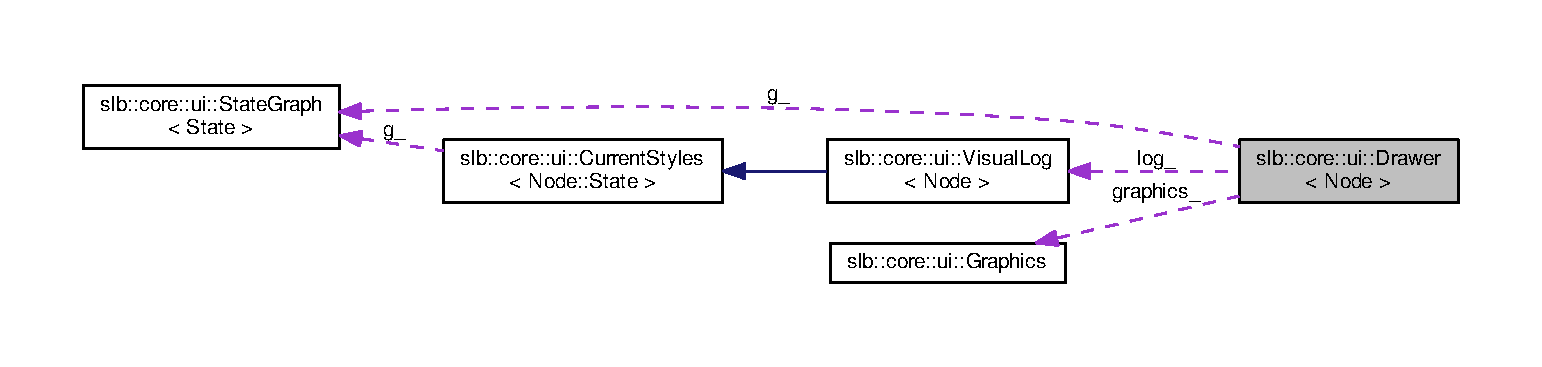
\includegraphics[width=350pt]{structslb_1_1core_1_1ui_1_1Drawer__coll__graph}
\end{center}
\end{figure}
\subsubsection*{Public Types}
\begin{DoxyCompactItemize}
\item 
using \hyperlink{structslb_1_1core_1_1ui_1_1Drawer_adf9110c216aa1d0a5080547a3bc22f06}{State} = typename Node\+::\+State\hypertarget{structslb_1_1core_1_1ui_1_1Drawer_adf9110c216aa1d0a5080547a3bc22f06}{}\label{structslb_1_1core_1_1ui_1_1Drawer_adf9110c216aa1d0a5080547a3bc22f06}

\begin{DoxyCompactList}\small\item\em The state type, represents the domain. \end{DoxyCompactList}\item 
using \hyperlink{structslb_1_1core_1_1ui_1_1Drawer_a70000b142df2f4e01123aa4bed5fd3a2}{Graph} = \hyperlink{structslb_1_1core_1_1ui_1_1StateGraph}{State\+Graph}$<$ \hyperlink{structslb_1_1core_1_1ui_1_1Drawer_adf9110c216aa1d0a5080547a3bc22f06}{State} $>$\hypertarget{structslb_1_1core_1_1ui_1_1Drawer_a70000b142df2f4e01123aa4bed5fd3a2}{}\label{structslb_1_1core_1_1ui_1_1Drawer_a70000b142df2f4e01123aa4bed5fd3a2}

\begin{DoxyCompactList}\small\item\em The domain graph type. \end{DoxyCompactList}\item 
using \hyperlink{structslb_1_1core_1_1ui_1_1Drawer_a1e0ed3482642e5d13e234f83bf690b8a}{My\+Visual\+Log} = \hyperlink{structslb_1_1core_1_1ui_1_1VisualLog}{Visual\+Log}$<$ Node $>$\hypertarget{structslb_1_1core_1_1ui_1_1Drawer_a1e0ed3482642e5d13e234f83bf690b8a}{}\label{structslb_1_1core_1_1ui_1_1Drawer_a1e0ed3482642e5d13e234f83bf690b8a}

\begin{DoxyCompactList}\small\item\em The log of visual events. \end{DoxyCompactList}\item 
using \hyperlink{structslb_1_1core_1_1ui_1_1Drawer_a3106bd6b1354ea4a24c3ef169c1e18b8}{Vertex\+Descriptor} = typename \hyperlink{structslb_1_1core_1_1ui_1_1StateGraph_ab2d88fce7d30dc6346910900212a7e6d}{Graph\+::\+Vertex\+Descriptor}\hypertarget{structslb_1_1core_1_1ui_1_1Drawer_a3106bd6b1354ea4a24c3ef169c1e18b8}{}\label{structslb_1_1core_1_1ui_1_1Drawer_a3106bd6b1354ea4a24c3ef169c1e18b8}

\begin{DoxyCompactList}\small\item\em Vertex identifier. \end{DoxyCompactList}\item 
using \hyperlink{structslb_1_1core_1_1ui_1_1Drawer_a77e84b439de5aa745cea48b184f060ec}{Point} = typename \hyperlink{structslb_1_1core_1_1ui_1_1StateGraph_a86d2316b03ddf9f3da4d6255d20a39d8}{Graph\+::\+Point}\hypertarget{structslb_1_1core_1_1ui_1_1Drawer_a77e84b439de5aa745cea48b184f060ec}{}\label{structslb_1_1core_1_1ui_1_1Drawer_a77e84b439de5aa745cea48b184f060ec}

\begin{DoxyCompactList}\small\item\em Type for vertex coordinates (used for computing the layout) \end{DoxyCompactList}\item 
using \hyperlink{structslb_1_1core_1_1ui_1_1Drawer_a5d8ae089b9b1f95a780bb1b0ef7d05e6}{Point\+Map} = typename \hyperlink{structslb_1_1core_1_1ui_1_1StateGraph_abc09edc649d6690817cb6219e3feefb0}{Graph\+::\+Point\+Map}\hypertarget{structslb_1_1core_1_1ui_1_1Drawer_a5d8ae089b9b1f95a780bb1b0ef7d05e6}{}\label{structslb_1_1core_1_1ui_1_1Drawer_a5d8ae089b9b1f95a780bb1b0ef7d05e6}

\begin{DoxyCompactList}\small\item\em Map for storing the layout, i.\+e. the coordinates of each vertex. \end{DoxyCompactList}\end{DoxyCompactItemize}
\subsubsection*{Public Member Functions}
\begin{DoxyCompactItemize}
\item 
\hyperlink{structslb_1_1core_1_1ui_1_1Drawer_a2b36937d5401aa35c7f72aadeaa84af8}{Drawer} (\hyperlink{structslb_1_1core_1_1ui_1_1Drawer_a70000b142df2f4e01123aa4bed5fd3a2}{Graph} \&g, const \hyperlink{structslb_1_1core_1_1ui_1_1Drawer_a1e0ed3482642e5d13e234f83bf690b8a}{My\+Visual\+Log} \&\hyperlink{namespaceslb_1_1core_1_1ui_acdeb0db1847459cac6f4eeb22bbb5998}{log})\hypertarget{structslb_1_1core_1_1ui_1_1Drawer_a2b36937d5401aa35c7f72aadeaa84af8}{}\label{structslb_1_1core_1_1ui_1_1Drawer_a2b36937d5401aa35c7f72aadeaa84af8}

\begin{DoxyCompactList}\small\item\em Initializes the drawer with the given (partial) domain graph and log of visual events. \end{DoxyCompactList}\item 
const \hyperlink{structslb_1_1core_1_1ui_1_1Drawer_a3106bd6b1354ea4a24c3ef169c1e18b8}{Vertex\+Descriptor} \hyperlink{structslb_1_1core_1_1ui_1_1Drawer_addc15f78ae4ec2bd61cdc5d5f61fa97e}{coords\+To\+VD} (double x, double y) const 
\begin{DoxyCompactList}\small\item\em Computes vertex in the (partial) domain graph based on point coordinates. This function is used to implement clickable vertices. \end{DoxyCompactList}\item 
void \hyperlink{structslb_1_1core_1_1ui_1_1Drawer_a9eac7f2468062e47c2ca24e988d74747}{make\+Layout} (bool draw\+Flag=false)
\begin{DoxyCompactList}\small\item\em Computes the layout of the (partial) domain graph and scales it to the current scale. \end{DoxyCompactList}\item 
\hyperlink{structslb_1_1core_1_1ui_1_1Graphics}{Graphics} \& \hyperlink{structslb_1_1core_1_1ui_1_1Drawer_af86e8fb465c1d617ea736012651a82e6}{graphics} ()
\begin{DoxyCompactList}\small\item\em Returns the graphics object. \end{DoxyCompactList}\item 
void \hyperlink{structslb_1_1core_1_1ui_1_1Drawer_a489ab8e47081333e9992a7b9f49222c6}{draw} ()\hypertarget{structslb_1_1core_1_1ui_1_1Drawer_a489ab8e47081333e9992a7b9f49222c6}{}\label{structslb_1_1core_1_1ui_1_1Drawer_a489ab8e47081333e9992a7b9f49222c6}

\begin{DoxyCompactList}\small\item\em Draws all vertices and edges with styles corresponding to the current state in the log of visual events. \end{DoxyCompactList}\item 
void \hyperlink{structslb_1_1core_1_1ui_1_1Drawer_ac6d8f7dde39ede250e0fbc3b04cc8eea}{draw\+Vertex} (\hyperlink{structslb_1_1core_1_1ui_1_1Drawer_a3106bd6b1354ea4a24c3ef169c1e18b8}{Vertex\+Descriptor} vd, const \hyperlink{structslb_1_1core_1_1ui_1_1VertexStyle}{Vertex\+Style} \&style)
\begin{DoxyCompactList}\small\item\em Draws the given vertex with the given representation style. \end{DoxyCompactList}\item 
void \hyperlink{structslb_1_1core_1_1ui_1_1Drawer_a685a55fbe52a5985fb3daf5379b2a702}{draw\+Vertex} (\hyperlink{structslb_1_1core_1_1ui_1_1Drawer_a3106bd6b1354ea4a24c3ef169c1e18b8}{Vertex\+Descriptor} vd)
\begin{DoxyCompactList}\small\item\em Draws the given vertex with the representation style corresponding to the current state of the log of visual events. \end{DoxyCompactList}\item 
void \hyperlink{structslb_1_1core_1_1ui_1_1Drawer_a703eb519af73b313173016941e21b985}{draw\+Edge} (\hyperlink{structslb_1_1core_1_1ui_1_1Drawer_a3106bd6b1354ea4a24c3ef169c1e18b8}{Vertex\+Descriptor} from, \hyperlink{structslb_1_1core_1_1ui_1_1Drawer_a3106bd6b1354ea4a24c3ef169c1e18b8}{Vertex\+Descriptor} to, const \hyperlink{structslb_1_1core_1_1ui_1_1EdgeStyle}{Edge\+Style} \&style)
\begin{DoxyCompactList}\small\item\em Draws the given edge with the given representation style. \end{DoxyCompactList}\item 
void \hyperlink{structslb_1_1core_1_1ui_1_1Drawer_aa30bec2103851daf685160efa904b447}{draw\+Edge} (\hyperlink{structslb_1_1core_1_1ui_1_1Drawer_a3106bd6b1354ea4a24c3ef169c1e18b8}{Vertex\+Descriptor} from, \hyperlink{structslb_1_1core_1_1ui_1_1Drawer_a3106bd6b1354ea4a24c3ef169c1e18b8}{Vertex\+Descriptor} to)
\begin{DoxyCompactList}\small\item\em Draws the given edge with the representation style corresponding to the current state of the log of visual events. \end{DoxyCompactList}\item 
void \hyperlink{structslb_1_1core_1_1ui_1_1Drawer_a34f3184f19e88390cfe24e95b1c6a41e}{show\+Labels} (bool flag)
\begin{DoxyCompactList}\small\item\em Sets the mode for either showing or hiding the labels. \end{DoxyCompactList}\end{DoxyCompactItemize}
\subsubsection*{Private Member Functions}
\begin{DoxyCompactItemize}
\item 
{\footnotesize template$<$class State  = State$>$ }\\\hyperlink{namespaceslb_1_1core_1_1ui_af200efa9fbb401dd541fa80e687e0264}{Has\+No\+Layout}$<$ \hyperlink{structslb_1_1core_1_1ui_1_1Drawer_adf9110c216aa1d0a5080547a3bc22f06}{State} $>$ \hyperlink{structslb_1_1core_1_1ui_1_1Drawer_adadbebe7db523e3888c6f740840cf7d2}{compute\+Point\+Map\+\_\+} ()
\begin{DoxyCompactList}\small\item\em Computes the automatic layout in the absence of the {\ttfamily visual\+Location} member function of {\ttfamily State}. \end{DoxyCompactList}\item 
{\footnotesize template$<$class State  = State$>$ }\\\hyperlink{namespaceslb_1_1core_1_1ui_a9bf16cc2a70201a2d10994dbffbe094f}{Has\+Layout}$<$ \hyperlink{structslb_1_1core_1_1ui_1_1Drawer_adf9110c216aa1d0a5080547a3bc22f06}{State} $>$ \hyperlink{structslb_1_1core_1_1ui_1_1Drawer_ae26d220bbf7e1c774570ff91dd57d68b}{compute\+Point\+Map\+\_\+} ()
\begin{DoxyCompactList}\small\item\em Computes the automatic layout using the {\ttfamily visual\+Location} member function of {\ttfamily State}. \end{DoxyCompactList}\item 
void \hyperlink{structslb_1_1core_1_1ui_1_1Drawer_ab7b5c9f69f03b5b5f515ab2db5c10d30}{fill\+Vertex} (\hyperlink{structslb_1_1core_1_1ui_1_1Drawer_a3106bd6b1354ea4a24c3ef169c1e18b8}{Vertex\+Descriptor} vd, const \hyperlink{structslb_1_1core_1_1ui_1_1VertexStyle}{Vertex\+Style} \&style)
\begin{DoxyCompactList}\small\item\em Fills inside the vertex according to the given style. \end{DoxyCompactList}\item 
void \hyperlink{structslb_1_1core_1_1ui_1_1Drawer_a897c99eafc0805ec03b876290c39b4c4}{emphasize\+Vertex} (\hyperlink{structslb_1_1core_1_1ui_1_1Drawer_a3106bd6b1354ea4a24c3ef169c1e18b8}{Vertex\+Descriptor} vd, const \hyperlink{structslb_1_1core_1_1ui_1_1VertexStyle}{Vertex\+Style} \&style)
\begin{DoxyCompactList}\small\item\em Draws the emphasis mark of the vertex (if there is one) according to the given style. \end{DoxyCompactList}\item 
void \hyperlink{structslb_1_1core_1_1ui_1_1Drawer_a0f55c8f860997d54043f4ec9b3dc9e34}{label\+Vertex} (\hyperlink{structslb_1_1core_1_1ui_1_1Drawer_a3106bd6b1354ea4a24c3ef169c1e18b8}{Vertex\+Descriptor} vd, const \hyperlink{structslb_1_1core_1_1ui_1_1VertexStyle}{Vertex\+Style} \&style)
\begin{DoxyCompactList}\small\item\em Labels the vertex. \end{DoxyCompactList}\item 
void \hyperlink{structslb_1_1core_1_1ui_1_1Drawer_af4549706b49ae5134b017a42e34edfa5}{label\+Edge} (\hyperlink{structslb_1_1core_1_1ui_1_1Drawer_a3106bd6b1354ea4a24c3ef169c1e18b8}{Vertex\+Descriptor} from, \hyperlink{structslb_1_1core_1_1ui_1_1Drawer_a3106bd6b1354ea4a24c3ef169c1e18b8}{Vertex\+Descriptor} to, const \hyperlink{structslb_1_1core_1_1ui_1_1EdgeStyle}{Edge\+Style} \&style)
\begin{DoxyCompactList}\small\item\em Labels the edge. \end{DoxyCompactList}\item 
double \hyperlink{structslb_1_1core_1_1ui_1_1Drawer_a0c85b4e405d6caaaa660b361517c9196}{distance\+Percentile} (double p)
\begin{DoxyCompactList}\small\item\em Computes a p-\/percentile of edge pixel-\/lengths. p must be between 0 and 1. If p == 0, then the pixel-\/length of the shortest edge is returned. If p == 1, the pixel-\/length of the longest edge is returned. \end{DoxyCompactList}\item 
void \hyperlink{structslb_1_1core_1_1ui_1_1Drawer_a51558414e4dc38d3e879d2ed38b97f1d}{scale\+Layout\+\_\+} (int x, int y)\hypertarget{structslb_1_1core_1_1ui_1_1Drawer_a51558414e4dc38d3e879d2ed38b97f1d}{}\label{structslb_1_1core_1_1ui_1_1Drawer_a51558414e4dc38d3e879d2ed38b97f1d}

\begin{DoxyCompactList}\small\item\em Scales the layout (i.\+e. modified \hyperlink{structslb_1_1core_1_1ui_1_1Drawer_a3744c0f39a867c7a09cc079b775e22a3}{point\+Map\+\_\+}) to the given dimensions. The new x-\/dimension of the drawing. The new y-\/dimension of the drawing. \end{DoxyCompactList}\item 
void \hyperlink{structslb_1_1core_1_1ui_1_1Drawer_ae87b616f678ecb0fc818c8002d338881}{dump\+Layout} ()\hypertarget{structslb_1_1core_1_1ui_1_1Drawer_ae87b616f678ecb0fc818c8002d338881}{}\label{structslb_1_1core_1_1ui_1_1Drawer_ae87b616f678ecb0fc818c8002d338881}

\begin{DoxyCompactList}\small\item\em Dumps the layout to stderr for debugging purposes. \end{DoxyCompactList}\end{DoxyCompactItemize}
\subsubsection*{Private Attributes}
\begin{DoxyCompactItemize}
\item 
\hyperlink{structslb_1_1core_1_1ui_1_1Drawer_a70000b142df2f4e01123aa4bed5fd3a2}{Graph} \& \hyperlink{structslb_1_1core_1_1ui_1_1Drawer_a153935449f0929292b4e9407dd260d42}{g\+\_\+}\hypertarget{structslb_1_1core_1_1ui_1_1Drawer_a153935449f0929292b4e9407dd260d42}{}\label{structslb_1_1core_1_1ui_1_1Drawer_a153935449f0929292b4e9407dd260d42}

\begin{DoxyCompactList}\small\item\em The (partial) domain graph. \end{DoxyCompactList}\item 
const \hyperlink{structslb_1_1core_1_1ui_1_1Drawer_a1e0ed3482642e5d13e234f83bf690b8a}{My\+Visual\+Log} \& \hyperlink{structslb_1_1core_1_1ui_1_1Drawer_a968565e997ae415bc7c30aafdc93529e}{log\+\_\+}\hypertarget{structslb_1_1core_1_1ui_1_1Drawer_a968565e997ae415bc7c30aafdc93529e}{}\label{structslb_1_1core_1_1ui_1_1Drawer_a968565e997ae415bc7c30aafdc93529e}

\begin{DoxyCompactList}\small\item\em The log of visual events. \end{DoxyCompactList}\item 
\hyperlink{structslb_1_1core_1_1ui_1_1Drawer_a5d8ae089b9b1f95a780bb1b0ef7d05e6}{Point\+Map} \hyperlink{structslb_1_1core_1_1ui_1_1Drawer_a3744c0f39a867c7a09cc079b775e22a3}{point\+Map\+\_\+}\hypertarget{structslb_1_1core_1_1ui_1_1Drawer_a3744c0f39a867c7a09cc079b775e22a3}{}\label{structslb_1_1core_1_1ui_1_1Drawer_a3744c0f39a867c7a09cc079b775e22a3}

\begin{DoxyCompactList}\small\item\em The layout. \end{DoxyCompactList}\item 
\hyperlink{structslb_1_1core_1_1ui_1_1Graphics}{Graphics} \hyperlink{structslb_1_1core_1_1ui_1_1Drawer_ad90d552a5024e6f11a7b622a17f117b5}{graphics\+\_\+}\hypertarget{structslb_1_1core_1_1ui_1_1Drawer_ad90d552a5024e6f11a7b622a17f117b5}{}\label{structslb_1_1core_1_1ui_1_1Drawer_ad90d552a5024e6f11a7b622a17f117b5}

\begin{DoxyCompactList}\small\item\em The graphics object holding all the information needed for drawing. \end{DoxyCompactList}\item 
bool \hyperlink{structslb_1_1core_1_1ui_1_1Drawer_a580db97e1c2261304eaa4dc63fb22c60}{show\+Labels\+\_\+} = false\hypertarget{structslb_1_1core_1_1ui_1_1Drawer_a580db97e1c2261304eaa4dc63fb22c60}{}\label{structslb_1_1core_1_1ui_1_1Drawer_a580db97e1c2261304eaa4dc63fb22c60}

\begin{DoxyCompactList}\small\item\em Indicates wither the vertex and edge labels should be shown. \end{DoxyCompactList}\end{DoxyCompactItemize}


\subsubsection{Detailed Description}
\subsubsection*{template$<$class Node$>$\\*
struct slb\+::core\+::ui\+::\+Drawer$<$ Node $>$}

Draws the (partial) domain graph with given styles for visual representation of vertices and edges. 


\begin{DoxyTemplParams}{Template Parameters}
{\em Node} & The search node type, which is used here to refer to the visual log. \\
\hline
\end{DoxyTemplParams}


Definition at line 44 of file drawer.\+h.



\subsubsection{Member Function Documentation}
\index{slb\+::core\+::ui\+::\+Drawer@{slb\+::core\+::ui\+::\+Drawer}!compute\+Point\+Map\+\_\+@{compute\+Point\+Map\+\_\+}}
\index{compute\+Point\+Map\+\_\+@{compute\+Point\+Map\+\_\+}!slb\+::core\+::ui\+::\+Drawer@{slb\+::core\+::ui\+::\+Drawer}}
\paragraph[{\texorpdfstring{compute\+Point\+Map\+\_\+()}{computePointMap_()}}]{\setlength{\rightskip}{0pt plus 5cm}template$<$class Node $>$ template$<$class State  = State$>$ {\bf Has\+No\+Layout}$<${\bf State}$>$ {\bf slb\+::core\+::ui\+::\+Drawer}$<$ Node $>$\+::compute\+Point\+Map\+\_\+ (
\begin{DoxyParamCaption}
{}
\end{DoxyParamCaption}
)\hspace{0.3cm}{\ttfamily [inline]}, {\ttfamily [private]}}\hypertarget{structslb_1_1core_1_1ui_1_1Drawer_adadbebe7db523e3888c6f740840cf7d2}{}\label{structslb_1_1core_1_1ui_1_1Drawer_adadbebe7db523e3888c6f740840cf7d2}


Computes the automatic layout in the absence of the {\ttfamily visual\+Location} member function of {\ttfamily State}. 


\begin{DoxyTemplParams}{Template Parameters}
{\em State} & The search state type. \\
\hline
\end{DoxyTemplParams}
\begin{DoxyNote}{Note}
The return type is used for S\+F\+I\+N\+AE. It evaluates to {\ttfamily void}. 
\end{DoxyNote}


Definition at line 219 of file drawer.\+h.

\index{slb\+::core\+::ui\+::\+Drawer@{slb\+::core\+::ui\+::\+Drawer}!compute\+Point\+Map\+\_\+@{compute\+Point\+Map\+\_\+}}
\index{compute\+Point\+Map\+\_\+@{compute\+Point\+Map\+\_\+}!slb\+::core\+::ui\+::\+Drawer@{slb\+::core\+::ui\+::\+Drawer}}
\paragraph[{\texorpdfstring{compute\+Point\+Map\+\_\+()}{computePointMap_()}}]{\setlength{\rightskip}{0pt plus 5cm}template$<$class Node $>$ template$<$class State  = State$>$ {\bf Has\+Layout}$<${\bf State}$>$ {\bf slb\+::core\+::ui\+::\+Drawer}$<$ Node $>$\+::compute\+Point\+Map\+\_\+ (
\begin{DoxyParamCaption}
{}
\end{DoxyParamCaption}
)\hspace{0.3cm}{\ttfamily [inline]}, {\ttfamily [private]}}\hypertarget{structslb_1_1core_1_1ui_1_1Drawer_ae26d220bbf7e1c774570ff91dd57d68b}{}\label{structslb_1_1core_1_1ui_1_1Drawer_ae26d220bbf7e1c774570ff91dd57d68b}


Computes the automatic layout using the {\ttfamily visual\+Location} member function of {\ttfamily State}. 


\begin{DoxyTemplParams}{Template Parameters}
{\em State} & The search state type. \\
\hline
\end{DoxyTemplParams}
\begin{DoxyNote}{Note}
The return type is used for S\+F\+I\+N\+AE. It evaluates to {\ttfamily void}. 
\end{DoxyNote}


Definition at line 227 of file drawer.\+h.

\index{slb\+::core\+::ui\+::\+Drawer@{slb\+::core\+::ui\+::\+Drawer}!coords\+To\+VD@{coords\+To\+VD}}
\index{coords\+To\+VD@{coords\+To\+VD}!slb\+::core\+::ui\+::\+Drawer@{slb\+::core\+::ui\+::\+Drawer}}
\paragraph[{\texorpdfstring{coords\+To\+V\+D(double x, double y) const }{coordsToVD(double x, double y) const }}]{\setlength{\rightskip}{0pt plus 5cm}template$<$class Node $>$ const {\bf Vertex\+Descriptor} {\bf slb\+::core\+::ui\+::\+Drawer}$<$ Node $>$\+::coords\+To\+VD (
\begin{DoxyParamCaption}
\item[{double}]{x, }
\item[{double}]{y}
\end{DoxyParamCaption}
) const\hspace{0.3cm}{\ttfamily [inline]}}\hypertarget{structslb_1_1core_1_1ui_1_1Drawer_addc15f78ae4ec2bd61cdc5d5f61fa97e}{}\label{structslb_1_1core_1_1ui_1_1Drawer_addc15f78ae4ec2bd61cdc5d5f61fa97e}


Computes vertex in the (partial) domain graph based on point coordinates. This function is used to implement clickable vertices. 


\begin{DoxyParams}{Parameters}
{\em x} & The x-\/coordinate. \\
\hline
{\em y} & The y-\/coordinate. \\
\hline
\end{DoxyParams}
\begin{DoxyReturn}{Returns}
Identifier of the vertex corresponding to the given coordinates. If there is no corresponding vertex, {\ttfamily nullptr} is returned. 
\end{DoxyReturn}


Definition at line 75 of file drawer.\+h.

\index{slb\+::core\+::ui\+::\+Drawer@{slb\+::core\+::ui\+::\+Drawer}!distance\+Percentile@{distance\+Percentile}}
\index{distance\+Percentile@{distance\+Percentile}!slb\+::core\+::ui\+::\+Drawer@{slb\+::core\+::ui\+::\+Drawer}}
\paragraph[{\texorpdfstring{distance\+Percentile(double p)}{distancePercentile(double p)}}]{\setlength{\rightskip}{0pt plus 5cm}template$<$class Node $>$ double {\bf slb\+::core\+::ui\+::\+Drawer}$<$ Node $>$\+::distance\+Percentile (
\begin{DoxyParamCaption}
\item[{double}]{p}
\end{DoxyParamCaption}
)\hspace{0.3cm}{\ttfamily [inline]}, {\ttfamily [private]}}\hypertarget{structslb_1_1core_1_1ui_1_1Drawer_a0c85b4e405d6caaaa660b361517c9196}{}\label{structslb_1_1core_1_1ui_1_1Drawer_a0c85b4e405d6caaaa660b361517c9196}


Computes a p-\/percentile of edge pixel-\/lengths. p must be between 0 and 1. If p == 0, then the pixel-\/length of the shortest edge is returned. If p == 1, the pixel-\/length of the longest edge is returned. 

\begin{DoxyReturn}{Returns}
The p-\/percentile of edge pixel-\/lengths. 
\end{DoxyReturn}


Definition at line 334 of file drawer.\+h.

\index{slb\+::core\+::ui\+::\+Drawer@{slb\+::core\+::ui\+::\+Drawer}!draw\+Edge@{draw\+Edge}}
\index{draw\+Edge@{draw\+Edge}!slb\+::core\+::ui\+::\+Drawer@{slb\+::core\+::ui\+::\+Drawer}}
\paragraph[{\texorpdfstring{draw\+Edge(\+Vertex\+Descriptor from, Vertex\+Descriptor to, const Edge\+Style \&style)}{drawEdge(VertexDescriptor from, VertexDescriptor to, const EdgeStyle &style)}}]{\setlength{\rightskip}{0pt plus 5cm}template$<$class Node $>$ void {\bf slb\+::core\+::ui\+::\+Drawer}$<$ Node $>$\+::draw\+Edge (
\begin{DoxyParamCaption}
\item[{{\bf Vertex\+Descriptor}}]{from, }
\item[{{\bf Vertex\+Descriptor}}]{to, }
\item[{const {\bf Edge\+Style} \&}]{style}
\end{DoxyParamCaption}
)\hspace{0.3cm}{\ttfamily [inline]}}\hypertarget{structslb_1_1core_1_1ui_1_1Drawer_a703eb519af73b313173016941e21b985}{}\label{structslb_1_1core_1_1ui_1_1Drawer_a703eb519af73b313173016941e21b985}


Draws the given edge with the given representation style. 


\begin{DoxyParams}{Parameters}
{\em from} & The edge-\/source vertex identifier. \\
\hline
{\em to} & The edge-\/target vertex identifier. \\
\hline
{\em style} & The visual representation style. \\
\hline
\end{DoxyParams}


Definition at line 155 of file drawer.\+h.

\index{slb\+::core\+::ui\+::\+Drawer@{slb\+::core\+::ui\+::\+Drawer}!draw\+Edge@{draw\+Edge}}
\index{draw\+Edge@{draw\+Edge}!slb\+::core\+::ui\+::\+Drawer@{slb\+::core\+::ui\+::\+Drawer}}
\paragraph[{\texorpdfstring{draw\+Edge(\+Vertex\+Descriptor from, Vertex\+Descriptor to)}{drawEdge(VertexDescriptor from, VertexDescriptor to)}}]{\setlength{\rightskip}{0pt plus 5cm}template$<$class Node $>$ void {\bf slb\+::core\+::ui\+::\+Drawer}$<$ Node $>$\+::draw\+Edge (
\begin{DoxyParamCaption}
\item[{{\bf Vertex\+Descriptor}}]{from, }
\item[{{\bf Vertex\+Descriptor}}]{to}
\end{DoxyParamCaption}
)\hspace{0.3cm}{\ttfamily [inline]}}\hypertarget{structslb_1_1core_1_1ui_1_1Drawer_aa30bec2103851daf685160efa904b447}{}\label{structslb_1_1core_1_1ui_1_1Drawer_aa30bec2103851daf685160efa904b447}


Draws the given edge with the representation style corresponding to the current state of the log of visual events. 


\begin{DoxyParams}{Parameters}
{\em from} & The edge-\/source vertex identifier. \\
\hline
{\em to} & The edge-\/target vertex identifier. \\
\hline
\end{DoxyParams}


Definition at line 186 of file drawer.\+h.

\index{slb\+::core\+::ui\+::\+Drawer@{slb\+::core\+::ui\+::\+Drawer}!draw\+Vertex@{draw\+Vertex}}
\index{draw\+Vertex@{draw\+Vertex}!slb\+::core\+::ui\+::\+Drawer@{slb\+::core\+::ui\+::\+Drawer}}
\paragraph[{\texorpdfstring{draw\+Vertex(\+Vertex\+Descriptor vd, const Vertex\+Style \&style)}{drawVertex(VertexDescriptor vd, const VertexStyle &style)}}]{\setlength{\rightskip}{0pt plus 5cm}template$<$class Node $>$ void {\bf slb\+::core\+::ui\+::\+Drawer}$<$ Node $>$\+::draw\+Vertex (
\begin{DoxyParamCaption}
\item[{{\bf Vertex\+Descriptor}}]{vd, }
\item[{const {\bf Vertex\+Style} \&}]{style}
\end{DoxyParamCaption}
)\hspace{0.3cm}{\ttfamily [inline]}}\hypertarget{structslb_1_1core_1_1ui_1_1Drawer_ac6d8f7dde39ede250e0fbc3b04cc8eea}{}\label{structslb_1_1core_1_1ui_1_1Drawer_ac6d8f7dde39ede250e0fbc3b04cc8eea}


Draws the given vertex with the given representation style. 


\begin{DoxyParams}{Parameters}
{\em vd} & The vertex identifier. \\
\hline
{\em style} & The visual representation style. \\
\hline
\end{DoxyParams}


Definition at line 139 of file drawer.\+h.

\index{slb\+::core\+::ui\+::\+Drawer@{slb\+::core\+::ui\+::\+Drawer}!draw\+Vertex@{draw\+Vertex}}
\index{draw\+Vertex@{draw\+Vertex}!slb\+::core\+::ui\+::\+Drawer@{slb\+::core\+::ui\+::\+Drawer}}
\paragraph[{\texorpdfstring{draw\+Vertex(\+Vertex\+Descriptor vd)}{drawVertex(VertexDescriptor vd)}}]{\setlength{\rightskip}{0pt plus 5cm}template$<$class Node $>$ void {\bf slb\+::core\+::ui\+::\+Drawer}$<$ Node $>$\+::draw\+Vertex (
\begin{DoxyParamCaption}
\item[{{\bf Vertex\+Descriptor}}]{vd}
\end{DoxyParamCaption}
)\hspace{0.3cm}{\ttfamily [inline]}}\hypertarget{structslb_1_1core_1_1ui_1_1Drawer_a685a55fbe52a5985fb3daf5379b2a702}{}\label{structslb_1_1core_1_1ui_1_1Drawer_a685a55fbe52a5985fb3daf5379b2a702}


Draws the given vertex with the representation style corresponding to the current state of the log of visual events. 


\begin{DoxyParams}{Parameters}
{\em vd} & The vertex identifier. \\
\hline
\end{DoxyParams}


Definition at line 149 of file drawer.\+h.

\index{slb\+::core\+::ui\+::\+Drawer@{slb\+::core\+::ui\+::\+Drawer}!emphasize\+Vertex@{emphasize\+Vertex}}
\index{emphasize\+Vertex@{emphasize\+Vertex}!slb\+::core\+::ui\+::\+Drawer@{slb\+::core\+::ui\+::\+Drawer}}
\paragraph[{\texorpdfstring{emphasize\+Vertex(\+Vertex\+Descriptor vd, const Vertex\+Style \&style)}{emphasizeVertex(VertexDescriptor vd, const VertexStyle &style)}}]{\setlength{\rightskip}{0pt plus 5cm}template$<$class Node $>$ void {\bf slb\+::core\+::ui\+::\+Drawer}$<$ Node $>$\+::emphasize\+Vertex (
\begin{DoxyParamCaption}
\item[{{\bf Vertex\+Descriptor}}]{vd, }
\item[{const {\bf Vertex\+Style} \&}]{style}
\end{DoxyParamCaption}
)\hspace{0.3cm}{\ttfamily [inline]}, {\ttfamily [private]}}\hypertarget{structslb_1_1core_1_1ui_1_1Drawer_a897c99eafc0805ec03b876290c39b4c4}{}\label{structslb_1_1core_1_1ui_1_1Drawer_a897c99eafc0805ec03b876290c39b4c4}


Draws the emphasis mark of the vertex (if there is one) according to the given style. 


\begin{DoxyParams}{Parameters}
{\em vd} & The vertex identifier. \\
\hline
{\em style} & The visual presentation style for the vertex. \\
\hline
\end{DoxyParams}


Definition at line 265 of file drawer.\+h.

\index{slb\+::core\+::ui\+::\+Drawer@{slb\+::core\+::ui\+::\+Drawer}!fill\+Vertex@{fill\+Vertex}}
\index{fill\+Vertex@{fill\+Vertex}!slb\+::core\+::ui\+::\+Drawer@{slb\+::core\+::ui\+::\+Drawer}}
\paragraph[{\texorpdfstring{fill\+Vertex(\+Vertex\+Descriptor vd, const Vertex\+Style \&style)}{fillVertex(VertexDescriptor vd, const VertexStyle &style)}}]{\setlength{\rightskip}{0pt plus 5cm}template$<$class Node $>$ void {\bf slb\+::core\+::ui\+::\+Drawer}$<$ Node $>$\+::fill\+Vertex (
\begin{DoxyParamCaption}
\item[{{\bf Vertex\+Descriptor}}]{vd, }
\item[{const {\bf Vertex\+Style} \&}]{style}
\end{DoxyParamCaption}
)\hspace{0.3cm}{\ttfamily [inline]}, {\ttfamily [private]}}\hypertarget{structslb_1_1core_1_1ui_1_1Drawer_ab7b5c9f69f03b5b5f515ab2db5c10d30}{}\label{structslb_1_1core_1_1ui_1_1Drawer_ab7b5c9f69f03b5b5f515ab2db5c10d30}


Fills inside the vertex according to the given style. 


\begin{DoxyParams}{Parameters}
{\em vd} & The vertex identifier. \\
\hline
{\em style} & The visual presentation style for the vertex. \\
\hline
\end{DoxyParams}


Definition at line 242 of file drawer.\+h.

\index{slb\+::core\+::ui\+::\+Drawer@{slb\+::core\+::ui\+::\+Drawer}!graphics@{graphics}}
\index{graphics@{graphics}!slb\+::core\+::ui\+::\+Drawer@{slb\+::core\+::ui\+::\+Drawer}}
\paragraph[{\texorpdfstring{graphics()}{graphics()}}]{\setlength{\rightskip}{0pt plus 5cm}template$<$class Node $>$ {\bf Graphics}\& {\bf slb\+::core\+::ui\+::\+Drawer}$<$ Node $>$\+::graphics (
\begin{DoxyParamCaption}
{}
\end{DoxyParamCaption}
)\hspace{0.3cm}{\ttfamily [inline]}}\hypertarget{structslb_1_1core_1_1ui_1_1Drawer_af86e8fb465c1d617ea736012651a82e6}{}\label{structslb_1_1core_1_1ui_1_1Drawer_af86e8fb465c1d617ea736012651a82e6}


Returns the graphics object. 

\begin{DoxyReturn}{Returns}
Reference to the graphics object. 
\end{DoxyReturn}


Definition at line 108 of file drawer.\+h.

\index{slb\+::core\+::ui\+::\+Drawer@{slb\+::core\+::ui\+::\+Drawer}!label\+Edge@{label\+Edge}}
\index{label\+Edge@{label\+Edge}!slb\+::core\+::ui\+::\+Drawer@{slb\+::core\+::ui\+::\+Drawer}}
\paragraph[{\texorpdfstring{label\+Edge(\+Vertex\+Descriptor from, Vertex\+Descriptor to, const Edge\+Style \&style)}{labelEdge(VertexDescriptor from, VertexDescriptor to, const EdgeStyle &style)}}]{\setlength{\rightskip}{0pt plus 5cm}template$<$class Node $>$ void {\bf slb\+::core\+::ui\+::\+Drawer}$<$ Node $>$\+::label\+Edge (
\begin{DoxyParamCaption}
\item[{{\bf Vertex\+Descriptor}}]{from, }
\item[{{\bf Vertex\+Descriptor}}]{to, }
\item[{const {\bf Edge\+Style} \&}]{style}
\end{DoxyParamCaption}
)\hspace{0.3cm}{\ttfamily [inline]}, {\ttfamily [private]}}\hypertarget{structslb_1_1core_1_1ui_1_1Drawer_af4549706b49ae5134b017a42e34edfa5}{}\label{structslb_1_1core_1_1ui_1_1Drawer_af4549706b49ae5134b017a42e34edfa5}


Labels the edge. 


\begin{DoxyParams}{Parameters}
{\em from} & The edge-\/source vertex identifier. \\
\hline
{\em to} & The edge-\/target vertex identifier. \\
\hline
{\em style} & The visual representation style. \\
\hline
\end{DoxyParams}


Definition at line 309 of file drawer.\+h.

\index{slb\+::core\+::ui\+::\+Drawer@{slb\+::core\+::ui\+::\+Drawer}!label\+Vertex@{label\+Vertex}}
\index{label\+Vertex@{label\+Vertex}!slb\+::core\+::ui\+::\+Drawer@{slb\+::core\+::ui\+::\+Drawer}}
\paragraph[{\texorpdfstring{label\+Vertex(\+Vertex\+Descriptor vd, const Vertex\+Style \&style)}{labelVertex(VertexDescriptor vd, const VertexStyle &style)}}]{\setlength{\rightskip}{0pt plus 5cm}template$<$class Node $>$ void {\bf slb\+::core\+::ui\+::\+Drawer}$<$ Node $>$\+::label\+Vertex (
\begin{DoxyParamCaption}
\item[{{\bf Vertex\+Descriptor}}]{vd, }
\item[{const {\bf Vertex\+Style} \&}]{style}
\end{DoxyParamCaption}
)\hspace{0.3cm}{\ttfamily [inline]}, {\ttfamily [private]}}\hypertarget{structslb_1_1core_1_1ui_1_1Drawer_a0f55c8f860997d54043f4ec9b3dc9e34}{}\label{structslb_1_1core_1_1ui_1_1Drawer_a0f55c8f860997d54043f4ec9b3dc9e34}


Labels the vertex. 


\begin{DoxyParams}{Parameters}
{\em vd} & The vertex identifier. \\
\hline
{\em style} & The visual presentation style for the vertex. \\
\hline
\end{DoxyParams}


Definition at line 287 of file drawer.\+h.

\index{slb\+::core\+::ui\+::\+Drawer@{slb\+::core\+::ui\+::\+Drawer}!make\+Layout@{make\+Layout}}
\index{make\+Layout@{make\+Layout}!slb\+::core\+::ui\+::\+Drawer@{slb\+::core\+::ui\+::\+Drawer}}
\paragraph[{\texorpdfstring{make\+Layout(bool draw\+Flag=false)}{makeLayout(bool drawFlag=false)}}]{\setlength{\rightskip}{0pt plus 5cm}template$<$class Node $>$ void {\bf slb\+::core\+::ui\+::\+Drawer}$<$ Node $>$\+::make\+Layout (
\begin{DoxyParamCaption}
\item[{bool}]{draw\+Flag = {\ttfamily false}}
\end{DoxyParamCaption}
)\hspace{0.3cm}{\ttfamily [inline]}}\hypertarget{structslb_1_1core_1_1ui_1_1Drawer_a9eac7f2468062e47c2ca24e988d74747}{}\label{structslb_1_1core_1_1ui_1_1Drawer_a9eac7f2468062e47c2ca24e988d74747}


Computes the layout of the (partial) domain graph and scales it to the current scale. 


\begin{DoxyParams}{Parameters}
{\em draw\+Flag} & If {\ttfamily true}, then \hyperlink{structslb_1_1core_1_1ui_1_1Drawer_a489ab8e47081333e9992a7b9f49222c6}{draw} is called. \\
\hline
\end{DoxyParams}


Definition at line 97 of file drawer.\+h.

\index{slb\+::core\+::ui\+::\+Drawer@{slb\+::core\+::ui\+::\+Drawer}!show\+Labels@{show\+Labels}}
\index{show\+Labels@{show\+Labels}!slb\+::core\+::ui\+::\+Drawer@{slb\+::core\+::ui\+::\+Drawer}}
\paragraph[{\texorpdfstring{show\+Labels(bool flag)}{showLabels(bool flag)}}]{\setlength{\rightskip}{0pt plus 5cm}template$<$class Node $>$ void {\bf slb\+::core\+::ui\+::\+Drawer}$<$ Node $>$\+::show\+Labels (
\begin{DoxyParamCaption}
\item[{bool}]{flag}
\end{DoxyParamCaption}
)\hspace{0.3cm}{\ttfamily [inline]}}\hypertarget{structslb_1_1core_1_1ui_1_1Drawer_a34f3184f19e88390cfe24e95b1c6a41e}{}\label{structslb_1_1core_1_1ui_1_1Drawer_a34f3184f19e88390cfe24e95b1c6a41e}


Sets the mode for either showing or hiding the labels. 


\begin{DoxyParams}{Parameters}
{\em flag} & If {\ttfamily true}, the labels will be shown. They will be hidden otherwise. \\
\hline
\end{DoxyParams}


Definition at line 197 of file drawer.\+h.



The documentation for this struct was generated from the following file\+:\begin{DoxyCompactItemize}
\item 
core/user\+\_\+interface/\hyperlink{drawer_8h}{drawer.\+h}\end{DoxyCompactItemize}

\hypertarget{structslb_1_1ext_1_1domain_1_1pancake_1_1DynamicGapHeuristic}{}\subsection{slb\+:\+:ext\+:\+:domain\+:\+:pancake\+:\+:Dynamic\+Gap\+Heuristic Struct Reference}
\label{structslb_1_1ext_1_1domain_1_1pancake_1_1DynamicGapHeuristic}\index{slb\+::ext\+::domain\+::pancake\+::\+Dynamic\+Gap\+Heuristic@{slb\+::ext\+::domain\+::pancake\+::\+Dynamic\+Gap\+Heuristic}}


Functor for computing the dynamic gap heuristic to the goal state with ordered pancakes.  




{\ttfamily \#include $<$pancake.\+h$>$}

\subsubsection*{Public Member Functions}
\begin{DoxyCompactItemize}
\item 
\hyperlink{structslb_1_1ext_1_1domain_1_1pancake_1_1DynamicGapHeuristic_a319fbfce78634255bb6b73a20a162fa7}{Dynamic\+Gap\+Heuristic} (const \hyperlink{structslb_1_1ext_1_1domain_1_1pancake_1_1Pancake}{Pancake} \&)\hypertarget{structslb_1_1ext_1_1domain_1_1pancake_1_1DynamicGapHeuristic_a319fbfce78634255bb6b73a20a162fa7}{}\label{structslb_1_1ext_1_1domain_1_1pancake_1_1DynamicGapHeuristic_a319fbfce78634255bb6b73a20a162fa7}

\begin{DoxyCompactList}\small\item\em The constructor. \end{DoxyCompactList}\item 
{\footnotesize template$<$class Neighbor $>$ }\\int \hyperlink{structslb_1_1ext_1_1domain_1_1pancake_1_1DynamicGapHeuristic_aa2f8656c3030bc740544f1e807fc46ae}{operator()} (const \hyperlink{structslb_1_1ext_1_1domain_1_1pancake_1_1Pancake}{Pancake} \&parent, \hyperlink{structslb_1_1ext_1_1domain_1_1pancake_1_1Pancake_a53aacc6af425f7650fdb94880b1c2572}{Pancake\+::\+Cost\+Type}, const Neighbor \&n) const 
\begin{DoxyCompactList}\small\item\em The call operator. Dynamically computes the gap heuristic that results from applying a given action. \end{DoxyCompactList}\end{DoxyCompactItemize}


\subsubsection{Detailed Description}
Functor for computing the dynamic gap heuristic to the goal state with ordered pancakes. 

Definition at line 242 of file pancake.\+h.



\subsubsection{Member Function Documentation}
\index{slb\+::ext\+::domain\+::pancake\+::\+Dynamic\+Gap\+Heuristic@{slb\+::ext\+::domain\+::pancake\+::\+Dynamic\+Gap\+Heuristic}!operator()@{operator()}}
\index{operator()@{operator()}!slb\+::ext\+::domain\+::pancake\+::\+Dynamic\+Gap\+Heuristic@{slb\+::ext\+::domain\+::pancake\+::\+Dynamic\+Gap\+Heuristic}}
\paragraph[{\texorpdfstring{operator()(const Pancake \&parent, Pancake\+::\+Cost\+Type, const Neighbor \&n) const }{operator()(const Pancake &parent, Pancake::CostType, const Neighbor &n) const }}]{\setlength{\rightskip}{0pt plus 5cm}template$<$class Neighbor $>$ int slb\+::ext\+::domain\+::pancake\+::\+Dynamic\+Gap\+Heuristic\+::operator() (
\begin{DoxyParamCaption}
\item[{const {\bf Pancake} \&}]{parent, }
\item[{{\bf Pancake\+::\+Cost\+Type}}]{, }
\item[{const Neighbor \&}]{n}
\end{DoxyParamCaption}
) const\hspace{0.3cm}{\ttfamily [inline]}}\hypertarget{structslb_1_1ext_1_1domain_1_1pancake_1_1DynamicGapHeuristic_aa2f8656c3030bc740544f1e807fc46ae}{}\label{structslb_1_1ext_1_1domain_1_1pancake_1_1DynamicGapHeuristic_aa2f8656c3030bc740544f1e807fc46ae}


The call operator. Dynamically computes the gap heuristic that results from applying a given action. 


\begin{DoxyParams}{Parameters}
{\em parent} & The parent state. \\
\hline
{\em n} & The neighbor. \\
\hline
\end{DoxyParams}


Definition at line 251 of file pancake.\+h.



The documentation for this struct was generated from the following file\+:\begin{DoxyCompactItemize}
\item 
extensions/domains/\hyperlink{pancake_8h}{pancake.\+h}\end{DoxyCompactItemize}

\hypertarget{structslb_1_1ext_1_1domain_1_1sliding__tile_1_1DynamicMDHeuristic}{}\subsection{slb\+:\+:ext\+:\+:domain\+:\+:sliding\+\_\+tile\+:\+:Dynamic\+M\+D\+Heuristic Struct Reference}
\label{structslb_1_1ext_1_1domain_1_1sliding__tile_1_1DynamicMDHeuristic}\index{slb\+::ext\+::domain\+::sliding\+\_\+tile\+::\+Dynamic\+M\+D\+Heuristic@{slb\+::ext\+::domain\+::sliding\+\_\+tile\+::\+Dynamic\+M\+D\+Heuristic}}


Functor for computing the dynamic Manhattan distance heuristic to the goal state with ordered pancakes and blank at position 0.  




{\ttfamily \#include $<$sliding\+\_\+tile.\+h$>$}

\subsubsection*{Public Member Functions}
\begin{DoxyCompactItemize}
\item 
{\footnotesize template$<$int n\+Rows, int n\+Columns$>$ }\\\hyperlink{structslb_1_1ext_1_1domain_1_1sliding__tile_1_1DynamicMDHeuristic_a5404b91da8e8562fbabe43e0a57d1ab6}{Dynamic\+M\+D\+Heuristic} (const \hyperlink{structslb_1_1ext_1_1domain_1_1sliding__tile_1_1SlidingTile}{Sliding\+Tile}$<$ n\+Rows, n\+Columns $>$ \&)\hypertarget{structslb_1_1ext_1_1domain_1_1sliding__tile_1_1DynamicMDHeuristic_a5404b91da8e8562fbabe43e0a57d1ab6}{}\label{structslb_1_1ext_1_1domain_1_1sliding__tile_1_1DynamicMDHeuristic_a5404b91da8e8562fbabe43e0a57d1ab6}

\begin{DoxyCompactList}\small\item\em The constructor. \end{DoxyCompactList}\item 
{\footnotesize template$<$class Neighbor , int n\+Rows, int n\+Columns$>$ }\\int \hyperlink{structslb_1_1ext_1_1domain_1_1sliding__tile_1_1DynamicMDHeuristic_ae0da625d0d9acb7d69b739d94a2fccab}{operator()} (const \hyperlink{structslb_1_1ext_1_1domain_1_1sliding__tile_1_1SlidingTile}{Sliding\+Tile}$<$ n\+Rows, n\+Columns $>$ \&parent, typename \hyperlink{structslb_1_1ext_1_1domain_1_1sliding__tile_1_1SlidingTile}{Sliding\+Tile}$<$ n\+Rows, n\+Columns $>$\+::Cost\+Type, const Neighbor \&n) const 
\begin{DoxyCompactList}\small\item\em The call operator. Dynamically computes the MD heuristic that results from applying a given action. \end{DoxyCompactList}\end{DoxyCompactItemize}


\subsubsection{Detailed Description}
Functor for computing the dynamic Manhattan distance heuristic to the goal state with ordered pancakes and blank at position 0. 

Definition at line 291 of file sliding\+\_\+tile.\+h.



\subsubsection{Member Function Documentation}
\index{slb\+::ext\+::domain\+::sliding\+\_\+tile\+::\+Dynamic\+M\+D\+Heuristic@{slb\+::ext\+::domain\+::sliding\+\_\+tile\+::\+Dynamic\+M\+D\+Heuristic}!operator()@{operator()}}
\index{operator()@{operator()}!slb\+::ext\+::domain\+::sliding\+\_\+tile\+::\+Dynamic\+M\+D\+Heuristic@{slb\+::ext\+::domain\+::sliding\+\_\+tile\+::\+Dynamic\+M\+D\+Heuristic}}
\paragraph[{\texorpdfstring{operator()(const Sliding\+Tile$<$ n\+Rows, n\+Columns $>$ \&parent, typename Sliding\+Tile$<$ n\+Rows, n\+Columns $>$\+::\+Cost\+Type, const Neighbor \&n) const }{operator()(const SlidingTile< nRows, nColumns > &parent, typename SlidingTile< nRows, nColumns >::CostType, const Neighbor &n) const }}]{\setlength{\rightskip}{0pt plus 5cm}template$<$class Neighbor , int n\+Rows, int n\+Columns$>$ int slb\+::ext\+::domain\+::sliding\+\_\+tile\+::\+Dynamic\+M\+D\+Heuristic\+::operator() (
\begin{DoxyParamCaption}
\item[{const {\bf Sliding\+Tile}$<$ n\+Rows, n\+Columns $>$ \&}]{parent, }
\item[{typename {\bf Sliding\+Tile}$<$ n\+Rows, n\+Columns $>$\+::Cost\+Type}]{, }
\item[{const Neighbor \&}]{n}
\end{DoxyParamCaption}
) const\hspace{0.3cm}{\ttfamily [inline]}}\hypertarget{structslb_1_1ext_1_1domain_1_1sliding__tile_1_1DynamicMDHeuristic_ae0da625d0d9acb7d69b739d94a2fccab}{}\label{structslb_1_1ext_1_1domain_1_1sliding__tile_1_1DynamicMDHeuristic_ae0da625d0d9acb7d69b739d94a2fccab}


The call operator. Dynamically computes the MD heuristic that results from applying a given action. 


\begin{DoxyParams}{Parameters}
{\em parent} & The parent state. \\
\hline
{\em n} & The neighbor. \\
\hline
\end{DoxyParams}


Definition at line 301 of file sliding\+\_\+tile.\+h.



The documentation for this struct was generated from the following file\+:\begin{DoxyCompactItemize}
\item 
extensions/domains/\hyperlink{sliding__tile_8h}{sliding\+\_\+tile.\+h}\end{DoxyCompactItemize}

\hypertarget{structslb_1_1ext_1_1policy_1_1heuristic_1_1DynamicSingleGoalT}{}\subsection{slb\+:\+:ext\+:\+:policy\+:\+:heuristic\+:\+:Dynamic\+Single\+GoalT$<$ My\+Algorithm, Base\+Heuristic $>$ Struct Template Reference}
\label{structslb_1_1ext_1_1policy_1_1heuristic_1_1DynamicSingleGoalT}\index{slb\+::ext\+::policy\+::heuristic\+::\+Dynamic\+Single\+Goal\+T$<$ My\+Algorithm, Base\+Heuristic $>$@{slb\+::ext\+::policy\+::heuristic\+::\+Dynamic\+Single\+Goal\+T$<$ My\+Algorithm, Base\+Heuristic $>$}}


Dynamic heuristic to single goal.  




{\ttfamily \#include $<$heuristic\+\_\+policies.\+h$>$}

\subsubsection*{Public Member Functions}
\begin{DoxyCompactItemize}
\item 
\hyperlink{extensions_2shared__policies_2headers_8h_ae70a06fa4631780beea14971eb36a562}{P\+O\+L\+I\+C\+Y\+\_\+\+T\+Y\+P\+ES} \hyperlink{structslb_1_1ext_1_1policy_1_1heuristic_1_1DynamicSingleGoalT_ab491e6a9a177935e45f3c0b93389a286}{Dynamic\+Single\+GoalT} (My\+Algorithm \&alg)
\begin{DoxyCompactList}\small\item\em The constructor. The goal state is taken from the algorithm by using the policy service. \end{DoxyCompactList}\item 
\hyperlink{structslb_1_1ext_1_1policy_1_1heuristic_1_1DynamicSingleGoalT_a97461ead765eae5d7f184641a832c9b1}{Dynamic\+Single\+GoalT} (My\+Algorithm \&alg, const State \&goal)
\begin{DoxyCompactList}\small\item\em The constructor with the goal state supplied as an argument. \end{DoxyCompactList}\item 
{\footnotesize template$<$class Neighbor $>$ }\\Cost\+Type \hyperlink{structslb_1_1ext_1_1policy_1_1heuristic_1_1DynamicSingleGoalT_ab2839e7036a9450c47aa91316afbaee1}{operator()} (const Neighbor \&n, Node $\ast$node) const 
\begin{DoxyCompactList}\small\item\em Computes the heuristic. \end{DoxyCompactList}\end{DoxyCompactItemize}
\subsubsection*{Private Attributes}
\begin{DoxyCompactItemize}
\item 
My\+Algorithm \& \hyperlink{structslb_1_1ext_1_1policy_1_1heuristic_1_1DynamicSingleGoalT_a026cda2674bdc44e0ccef60f63faa92f}{alg\+\_\+}\hypertarget{structslb_1_1ext_1_1policy_1_1heuristic_1_1DynamicSingleGoalT_a026cda2674bdc44e0ccef60f63faa92f}{}\label{structslb_1_1ext_1_1policy_1_1heuristic_1_1DynamicSingleGoalT_a026cda2674bdc44e0ccef60f63faa92f}

\begin{DoxyCompactList}\small\item\em The algorithm reference. \end{DoxyCompactList}\item 
Base\+Heuristic \hyperlink{structslb_1_1ext_1_1policy_1_1heuristic_1_1DynamicSingleGoalT_ae024f3749f1b97023f767267a07955f5}{heuristic\+\_\+}\hypertarget{structslb_1_1ext_1_1policy_1_1heuristic_1_1DynamicSingleGoalT_ae024f3749f1b97023f767267a07955f5}{}\label{structslb_1_1ext_1_1policy_1_1heuristic_1_1DynamicSingleGoalT_ae024f3749f1b97023f767267a07955f5}

\begin{DoxyCompactList}\small\item\em The underlying heuristic. \end{DoxyCompactList}\end{DoxyCompactItemize}


\subsubsection{Detailed Description}
\subsubsection*{template$<$class My\+Algorithm, class Base\+Heuristic = S\+L\+B\+\_\+\+B\+A\+S\+E\+\_\+\+D\+Y\+N\+A\+M\+I\+C\+\_\+\+H\+E\+U\+R\+I\+S\+T\+IC$>$\\*
struct slb\+::ext\+::policy\+::heuristic\+::\+Dynamic\+Single\+Goal\+T$<$ My\+Algorithm, Base\+Heuristic $>$}

Dynamic heuristic to single goal. 


\begin{DoxyTemplParams}{Template Parameters}
{\em My\+Algorithm} & The search algorithm. \\
\hline
{\em Base\+Heuristic} & The base heuristic type. \\
\hline
\end{DoxyTemplParams}


Definition at line 84 of file heuristic\+\_\+policies.\+h.



\subsubsection{Constructor \& Destructor Documentation}
\index{slb\+::ext\+::policy\+::heuristic\+::\+Dynamic\+Single\+GoalT@{slb\+::ext\+::policy\+::heuristic\+::\+Dynamic\+Single\+GoalT}!Dynamic\+Single\+GoalT@{Dynamic\+Single\+GoalT}}
\index{Dynamic\+Single\+GoalT@{Dynamic\+Single\+GoalT}!slb\+::ext\+::policy\+::heuristic\+::\+Dynamic\+Single\+GoalT@{slb\+::ext\+::policy\+::heuristic\+::\+Dynamic\+Single\+GoalT}}
\paragraph[{\texorpdfstring{Dynamic\+Single\+Goal\+T(\+My\+Algorithm \&alg)}{DynamicSingleGoalT(MyAlgorithm &alg)}}]{\setlength{\rightskip}{0pt plus 5cm}template$<$class My\+Algorithm , class Base\+Heuristic  = S\+L\+B\+\_\+\+B\+A\+S\+E\+\_\+\+D\+Y\+N\+A\+M\+I\+C\+\_\+\+H\+E\+U\+R\+I\+S\+T\+IC$>$ {\bf P\+O\+L\+I\+C\+Y\+\_\+\+T\+Y\+P\+ES} {\bf slb\+::ext\+::policy\+::heuristic\+::\+Dynamic\+Single\+GoalT}$<$ My\+Algorithm, Base\+Heuristic $>$\+::{\bf Dynamic\+Single\+GoalT} (
\begin{DoxyParamCaption}
\item[{My\+Algorithm \&}]{alg}
\end{DoxyParamCaption}
)\hspace{0.3cm}{\ttfamily [inline]}}\hypertarget{structslb_1_1ext_1_1policy_1_1heuristic_1_1DynamicSingleGoalT_ab491e6a9a177935e45f3c0b93389a286}{}\label{structslb_1_1ext_1_1policy_1_1heuristic_1_1DynamicSingleGoalT_ab491e6a9a177935e45f3c0b93389a286}


The constructor. The goal state is taken from the algorithm by using the policy service. 


\begin{DoxyParams}{Parameters}
{\em alg} & Reference to the algorithm \\
\hline
\end{DoxyParams}


Definition at line 89 of file heuristic\+\_\+policies.\+h.

\index{slb\+::ext\+::policy\+::heuristic\+::\+Dynamic\+Single\+GoalT@{slb\+::ext\+::policy\+::heuristic\+::\+Dynamic\+Single\+GoalT}!Dynamic\+Single\+GoalT@{Dynamic\+Single\+GoalT}}
\index{Dynamic\+Single\+GoalT@{Dynamic\+Single\+GoalT}!slb\+::ext\+::policy\+::heuristic\+::\+Dynamic\+Single\+GoalT@{slb\+::ext\+::policy\+::heuristic\+::\+Dynamic\+Single\+GoalT}}
\paragraph[{\texorpdfstring{Dynamic\+Single\+Goal\+T(\+My\+Algorithm \&alg, const State \&goal)}{DynamicSingleGoalT(MyAlgorithm &alg, const State &goal)}}]{\setlength{\rightskip}{0pt plus 5cm}template$<$class My\+Algorithm , class Base\+Heuristic  = S\+L\+B\+\_\+\+B\+A\+S\+E\+\_\+\+D\+Y\+N\+A\+M\+I\+C\+\_\+\+H\+E\+U\+R\+I\+S\+T\+IC$>$ {\bf slb\+::ext\+::policy\+::heuristic\+::\+Dynamic\+Single\+GoalT}$<$ My\+Algorithm, Base\+Heuristic $>$\+::{\bf Dynamic\+Single\+GoalT} (
\begin{DoxyParamCaption}
\item[{My\+Algorithm \&}]{alg, }
\item[{const State \&}]{goal}
\end{DoxyParamCaption}
)\hspace{0.3cm}{\ttfamily [inline]}}\hypertarget{structslb_1_1ext_1_1policy_1_1heuristic_1_1DynamicSingleGoalT_a97461ead765eae5d7f184641a832c9b1}{}\label{structslb_1_1ext_1_1policy_1_1heuristic_1_1DynamicSingleGoalT_a97461ead765eae5d7f184641a832c9b1}


The constructor with the goal state supplied as an argument. 


\begin{DoxyParams}{Parameters}
{\em alg} & Reference to the algorithm \\
\hline
{\em goal} & The goal state. \\
\hline
\end{DoxyParams}


Definition at line 94 of file heuristic\+\_\+policies.\+h.



\subsubsection{Member Function Documentation}
\index{slb\+::ext\+::policy\+::heuristic\+::\+Dynamic\+Single\+GoalT@{slb\+::ext\+::policy\+::heuristic\+::\+Dynamic\+Single\+GoalT}!operator()@{operator()}}
\index{operator()@{operator()}!slb\+::ext\+::policy\+::heuristic\+::\+Dynamic\+Single\+GoalT@{slb\+::ext\+::policy\+::heuristic\+::\+Dynamic\+Single\+GoalT}}
\paragraph[{\texorpdfstring{operator()(const Neighbor \&n, Node $\ast$node) const }{operator()(const Neighbor &n, Node *node) const }}]{\setlength{\rightskip}{0pt plus 5cm}template$<$class My\+Algorithm , class Base\+Heuristic  = S\+L\+B\+\_\+\+B\+A\+S\+E\+\_\+\+D\+Y\+N\+A\+M\+I\+C\+\_\+\+H\+E\+U\+R\+I\+S\+T\+IC$>$ template$<$class Neighbor $>$ Cost\+Type {\bf slb\+::ext\+::policy\+::heuristic\+::\+Dynamic\+Single\+GoalT}$<$ My\+Algorithm, Base\+Heuristic $>$\+::operator() (
\begin{DoxyParamCaption}
\item[{const Neighbor \&}]{n, }
\item[{Node $\ast$}]{node}
\end{DoxyParamCaption}
) const\hspace{0.3cm}{\ttfamily [inline]}}\hypertarget{structslb_1_1ext_1_1policy_1_1heuristic_1_1DynamicSingleGoalT_ab2839e7036a9450c47aa91316afbaee1}{}\label{structslb_1_1ext_1_1policy_1_1heuristic_1_1DynamicSingleGoalT_ab2839e7036a9450c47aa91316afbaee1}


Computes the heuristic. 


\begin{DoxyTemplParams}{Template Parameters}
{\em Neighbor} & The neighbor type. \\
\hline
\end{DoxyTemplParams}

\begin{DoxyParams}{Parameters}
{\em n} & The neighbor for which the heuristic is to be computed. \\
\hline
{\em node} & The search node. \\
\hline
\end{DoxyParams}
\begin{DoxyReturn}{Returns}
The heuristic value. 
\end{DoxyReturn}


Definition at line 102 of file heuristic\+\_\+policies.\+h.



The documentation for this struct was generated from the following file\+:\begin{DoxyCompactItemize}
\item 
extensions/shared\+\_\+policies/\hyperlink{heuristic__policies_8h}{heuristic\+\_\+policies.\+h}\end{DoxyCompactItemize}

\hypertarget{structslb_1_1core_1_1ui_1_1EventBase_1_1EdgeChange}{}\subsection{slb\+:\+:core\+:\+:ui\+:\+:Event\+Base$<$ Node $>$\+:\+:Edge\+Change Struct Reference}
\label{structslb_1_1core_1_1ui_1_1EventBase_1_1EdgeChange}\index{slb\+::core\+::ui\+::\+Event\+Base$<$ Node $>$\+::\+Edge\+Change@{slb\+::core\+::ui\+::\+Event\+Base$<$ Node $>$\+::\+Edge\+Change}}


Description of change of visual representation of an edge. An edge is represented here by a pair of smart pointers to states. Note that this is different from a visual event (see \hyperlink{structslb_1_1core_1_1ui_1_1VisualEvent_1_1EdgeChange}{Visual\+Event\+::\+Edge\+Change}), in which an edge is represented here by a pair of vertices of the domain graph.  




{\ttfamily \#include $<$event\+\_\+base.\+h$>$}



Collaboration diagram for slb\+:\+:core\+:\+:ui\+:\+:Event\+Base$<$ Node $>$\+:\+:Edge\+Change\+:\nopagebreak
\begin{figure}[H]
\begin{center}
\leavevmode
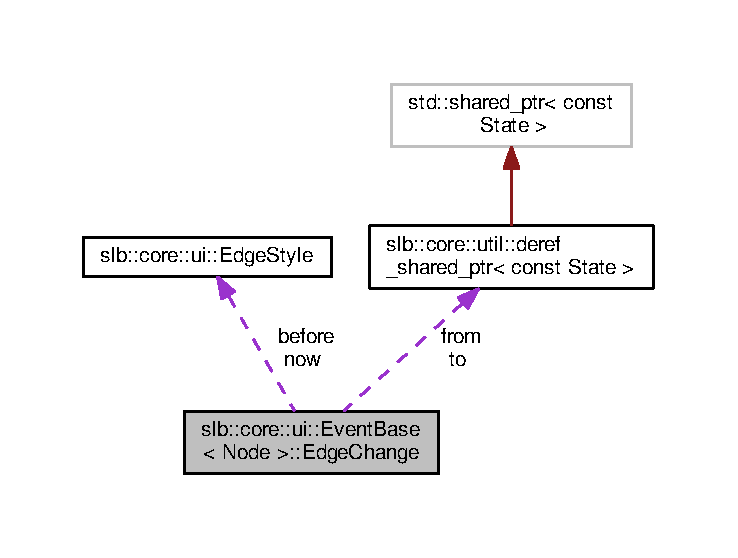
\includegraphics[width=350pt]{structslb_1_1core_1_1ui_1_1EventBase_1_1EdgeChange__coll__graph}
\end{center}
\end{figure}
\subsubsection*{Public Attributes}
\begin{DoxyCompactItemize}
\item 
\hyperlink{structslb_1_1core_1_1ui_1_1EventBase_a50419d00607aad434bb97138eabe2c94}{State\+Shared\+Ptr} \hyperlink{structslb_1_1core_1_1ui_1_1EventBase_1_1EdgeChange_ac18007f3e0545ad5437a60794a4ffe07}{from}\hypertarget{structslb_1_1core_1_1ui_1_1EventBase_1_1EdgeChange_ac18007f3e0545ad5437a60794a4ffe07}{}\label{structslb_1_1core_1_1ui_1_1EventBase_1_1EdgeChange_ac18007f3e0545ad5437a60794a4ffe07}

\begin{DoxyCompactList}\small\item\em The source state of the edge. \end{DoxyCompactList}\item 
\hyperlink{structslb_1_1core_1_1ui_1_1EventBase_a50419d00607aad434bb97138eabe2c94}{State\+Shared\+Ptr} \hyperlink{structslb_1_1core_1_1ui_1_1EventBase_1_1EdgeChange_a41cf618275848ca8701a4ad92f0100e7}{to}\hypertarget{structslb_1_1core_1_1ui_1_1EventBase_1_1EdgeChange_a41cf618275848ca8701a4ad92f0100e7}{}\label{structslb_1_1core_1_1ui_1_1EventBase_1_1EdgeChange_a41cf618275848ca8701a4ad92f0100e7}

\begin{DoxyCompactList}\small\item\em The target state of the edge. \end{DoxyCompactList}\item 
\hyperlink{structslb_1_1core_1_1ui_1_1EdgeStyle}{Edge\+Style} \hyperlink{structslb_1_1core_1_1ui_1_1EventBase_1_1EdgeChange_ab976192c4b6c3d561fc1165b7bdc9f6c}{now}\hypertarget{structslb_1_1core_1_1ui_1_1EventBase_1_1EdgeChange_ab976192c4b6c3d561fc1165b7bdc9f6c}{}\label{structslb_1_1core_1_1ui_1_1EventBase_1_1EdgeChange_ab976192c4b6c3d561fc1165b7bdc9f6c}

\begin{DoxyCompactList}\small\item\em The new representation. \end{DoxyCompactList}\item 
\hyperlink{structslb_1_1core_1_1ui_1_1EdgeStyle}{Edge\+Style} \hyperlink{structslb_1_1core_1_1ui_1_1EventBase_1_1EdgeChange_affa7e012f69870cc64f8ffdfa0f1ed9e}{before}\hypertarget{structslb_1_1core_1_1ui_1_1EventBase_1_1EdgeChange_affa7e012f69870cc64f8ffdfa0f1ed9e}{}\label{structslb_1_1core_1_1ui_1_1EventBase_1_1EdgeChange_affa7e012f69870cc64f8ffdfa0f1ed9e}

\begin{DoxyCompactList}\small\item\em The previous representation. \end{DoxyCompactList}\end{DoxyCompactItemize}


\subsubsection{Detailed Description}
\subsubsection*{template$<$class Node = S\+L\+B\+\_\+\+N\+O\+DE$>$\\*
struct slb\+::core\+::ui\+::\+Event\+Base$<$ Node $>$\+::\+Edge\+Change}

Description of change of visual representation of an edge. An edge is represented here by a pair of smart pointers to states. Note that this is different from a visual event (see \hyperlink{structslb_1_1core_1_1ui_1_1VisualEvent_1_1EdgeChange}{Visual\+Event\+::\+Edge\+Change}), in which an edge is represented here by a pair of vertices of the domain graph. 

Definition at line 56 of file event\+\_\+base.\+h.



The documentation for this struct was generated from the following file\+:\begin{DoxyCompactItemize}
\item 
core/user\+\_\+interface/\hyperlink{event__base_8h}{event\+\_\+base.\+h}\end{DoxyCompactItemize}

\hypertarget{structslb_1_1core_1_1ui_1_1VisualEvent_1_1EdgeChange}{}\subsection{slb\+:\+:core\+:\+:ui\+:\+:Visual\+Event$<$ State $>$\+:\+:Edge\+Change Struct Reference}
\label{structslb_1_1core_1_1ui_1_1VisualEvent_1_1EdgeChange}\index{slb\+::core\+::ui\+::\+Visual\+Event$<$ State $>$\+::\+Edge\+Change@{slb\+::core\+::ui\+::\+Visual\+Event$<$ State $>$\+::\+Edge\+Change}}


Description of change of visual representation of a single edge.  




{\ttfamily \#include $<$visual\+\_\+event.\+h$>$}



Collaboration diagram for slb\+:\+:core\+:\+:ui\+:\+:Visual\+Event$<$ State $>$\+:\+:Edge\+Change\+:\nopagebreak
\begin{figure}[H]
\begin{center}
\leavevmode
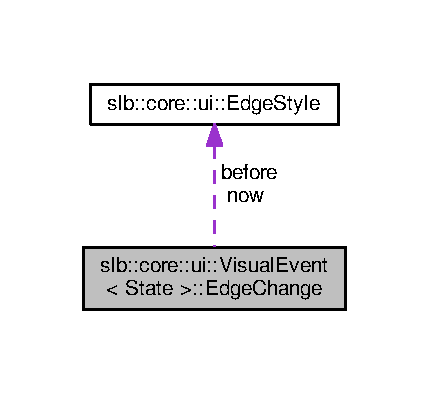
\includegraphics[width=206pt]{structslb_1_1core_1_1ui_1_1VisualEvent_1_1EdgeChange__coll__graph}
\end{center}
\end{figure}
\subsubsection*{Public Attributes}
\begin{DoxyCompactItemize}
\item 
Edge\+Descriptor \hyperlink{structslb_1_1core_1_1ui_1_1VisualEvent_1_1EdgeChange_a507204bfd9b20a7014d498e4c89c6d43}{ed}\hypertarget{structslb_1_1core_1_1ui_1_1VisualEvent_1_1EdgeChange_a507204bfd9b20a7014d498e4c89c6d43}{}\label{structslb_1_1core_1_1ui_1_1VisualEvent_1_1EdgeChange_a507204bfd9b20a7014d498e4c89c6d43}

\begin{DoxyCompactList}\small\item\em The edge identifier. \end{DoxyCompactList}\item 
\hyperlink{structslb_1_1core_1_1ui_1_1VisualEvent_ac004f17adad03549e2d7b07302e9c154}{Edge\+Style} \hyperlink{structslb_1_1core_1_1ui_1_1VisualEvent_1_1EdgeChange_a54f50a528016a4321b43dd9ffeb50edf}{now}\hypertarget{structslb_1_1core_1_1ui_1_1VisualEvent_1_1EdgeChange_a54f50a528016a4321b43dd9ffeb50edf}{}\label{structslb_1_1core_1_1ui_1_1VisualEvent_1_1EdgeChange_a54f50a528016a4321b43dd9ffeb50edf}

\begin{DoxyCompactList}\small\item\em The new representation. \end{DoxyCompactList}\item 
\hyperlink{structslb_1_1core_1_1ui_1_1VisualEvent_ac004f17adad03549e2d7b07302e9c154}{Edge\+Style} \hyperlink{structslb_1_1core_1_1ui_1_1VisualEvent_1_1EdgeChange_a9eb931a962fc08d955573df5a54b6e6a}{before}\hypertarget{structslb_1_1core_1_1ui_1_1VisualEvent_1_1EdgeChange_a9eb931a962fc08d955573df5a54b6e6a}{}\label{structslb_1_1core_1_1ui_1_1VisualEvent_1_1EdgeChange_a9eb931a962fc08d955573df5a54b6e6a}

\begin{DoxyCompactList}\small\item\em The previous representation. \end{DoxyCompactList}\end{DoxyCompactItemize}


\subsubsection{Detailed Description}
\subsubsection*{template$<$class State$>$\\*
struct slb\+::core\+::ui\+::\+Visual\+Event$<$ State $>$\+::\+Edge\+Change}

Description of change of visual representation of a single edge. 

Definition at line 36 of file visual\+\_\+event.\+h.



The documentation for this struct was generated from the following file\+:\begin{DoxyCompactItemize}
\item 
core/user\+\_\+interface/\hyperlink{visual__event_8h}{visual\+\_\+event.\+h}\end{DoxyCompactItemize}

\hypertarget{structslb_1_1core_1_1ui_1_1EdgeStyle}{}\subsection{slb\+:\+:core\+:\+:ui\+:\+:Edge\+Style Struct Reference}
\label{structslb_1_1core_1_1ui_1_1EdgeStyle}\index{slb\+::core\+::ui\+::\+Edge\+Style@{slb\+::core\+::ui\+::\+Edge\+Style}}


Visualization properties for a single directed edge.  




{\ttfamily \#include $<$style.\+h$>$}

\subsubsection*{Public Member Functions}
\begin{DoxyCompactItemize}
\item 
bool \hyperlink{structslb_1_1core_1_1ui_1_1EdgeStyle_aff7b9edc83714c44d13ce1582471ff3a}{operator==} (const \hyperlink{structslb_1_1core_1_1ui_1_1EdgeStyle}{Edge\+Style} \&rhs)\hypertarget{structslb_1_1core_1_1ui_1_1EdgeStyle_aff7b9edc83714c44d13ce1582471ff3a}{}\label{structslb_1_1core_1_1ui_1_1EdgeStyle_aff7b9edc83714c44d13ce1582471ff3a}

\begin{DoxyCompactList}\small\item\em Comparison of two edge styles. \end{DoxyCompactList}\end{DoxyCompactItemize}
\subsubsection*{Public Attributes}
\begin{DoxyCompactItemize}
\item 
\hyperlink{namespaceslb_1_1core_1_1util_afae144e1a65658559242f5cf4fce426f}{Color} \hyperlink{structslb_1_1core_1_1ui_1_1EdgeStyle_a651b7ec3c906e418f4d70c58cb280ca5}{color} = \hyperlink{structslb_1_1core_1_1ui_1_1EdgeStyle_a11590a49462e609a2fa986453f229fb7}{default\+Color}\hypertarget{structslb_1_1core_1_1ui_1_1EdgeStyle_a651b7ec3c906e418f4d70c58cb280ca5}{}\label{structslb_1_1core_1_1ui_1_1EdgeStyle_a651b7ec3c906e418f4d70c58cb280ca5}

\begin{DoxyCompactList}\small\item\em Edge color. \end{DoxyCompactList}\item 
double \hyperlink{structslb_1_1core_1_1ui_1_1EdgeStyle_a43492a2e8cee92017e7f9bfd6f3d0c26}{width\+Factor} = 1.\+0\hypertarget{structslb_1_1core_1_1ui_1_1EdgeStyle_a43492a2e8cee92017e7f9bfd6f3d0c26}{}\label{structslb_1_1core_1_1ui_1_1EdgeStyle_a43492a2e8cee92017e7f9bfd6f3d0c26}

\begin{DoxyCompactList}\small\item\em Width of the edge (in width\+Base units). \end{DoxyCompactList}\item 
bool \hyperlink{structslb_1_1core_1_1ui_1_1EdgeStyle_a16f86f80c24bd2c1941114a352424d55}{arrow} = false\hypertarget{structslb_1_1core_1_1ui_1_1EdgeStyle_a16f86f80c24bd2c1941114a352424d55}{}\label{structslb_1_1core_1_1ui_1_1EdgeStyle_a16f86f80c24bd2c1941114a352424d55}

\begin{DoxyCompactList}\small\item\em Whether the directed edge has an arrow to show the edge\textquotesingle{}s direction. \end{DoxyCompactList}\end{DoxyCompactItemize}
\subsubsection*{Static Public Attributes}
\begin{DoxyCompactItemize}
\item 
static constexpr \hyperlink{namespaceslb_1_1core_1_1util_afae144e1a65658559242f5cf4fce426f}{Color} \hyperlink{structslb_1_1core_1_1ui_1_1EdgeStyle_a11590a49462e609a2fa986453f229fb7}{default\+Color} = Color\+::\+B\+R\+O\+W\+N\+\_\+\+G\+R\+EY\hypertarget{structslb_1_1core_1_1ui_1_1EdgeStyle_a11590a49462e609a2fa986453f229fb7}{}\label{structslb_1_1core_1_1ui_1_1EdgeStyle_a11590a49462e609a2fa986453f229fb7}

\begin{DoxyCompactList}\small\item\em Color of an edge before an algorithm does something with it. \end{DoxyCompactList}\item 
static double \hyperlink{structslb_1_1core_1_1ui_1_1EdgeStyle_ad373481f2c46d147fd3658d5f217e2cf}{width\+Base} = 5.\+0\hypertarget{structslb_1_1core_1_1ui_1_1EdgeStyle_ad373481f2c46d147fd3658d5f217e2cf}{}\label{structslb_1_1core_1_1ui_1_1EdgeStyle_ad373481f2c46d147fd3658d5f217e2cf}

\begin{DoxyCompactList}\small\item\em Width corresponding to width\+Factor == 1.\+0. \end{DoxyCompactList}\end{DoxyCompactItemize}


\subsubsection{Detailed Description}
Visualization properties for a single directed edge. 

Definition at line 52 of file style.\+h.



The documentation for this struct was generated from the following file\+:\begin{DoxyCompactItemize}
\item 
core/user\+\_\+interface/\hyperlink{style_8h}{style.\+h}\end{DoxyCompactItemize}

\hypertarget{structslb_1_1core_1_1ui_1_1EditField}{}\subsection{slb\+:\+:core\+:\+:ui\+:\+:Edit\+Field Struct Reference}
\label{structslb_1_1core_1_1ui_1_1EditField}\index{slb\+::core\+::ui\+::\+Edit\+Field@{slb\+::core\+::ui\+::\+Edit\+Field}}


Implements a simple text edit field.  




{\ttfamily \#include $<$form.\+h$>$}

\subsubsection*{Public Member Functions}
\begin{DoxyCompactItemize}
\item 
\hyperlink{structslb_1_1core_1_1ui_1_1EditField_a607291bf49b0dca5cbff3bac7767f869}{Edit\+Field} (Display $\ast$\hyperlink{structslb_1_1core_1_1ui_1_1EditField_ab8483df66ec0bca8e5d59ea547113a04}{display}, W\+I\+N\+D\+OW $\ast$host, int begin\+Row, int begin\+Col, int nrows, int ncols, std\+::string label)
\begin{DoxyCompactList}\small\item\em Initializes the text field. \end{DoxyCompactList}\item 
const std\+::string \& \hyperlink{structslb_1_1core_1_1ui_1_1EditField_adc15bb0294ab839703a01da5bd8c6106}{get} () const 
\begin{DoxyCompactList}\small\item\em Returns the contents of the field. \end{DoxyCompactList}\item 
void \hyperlink{structslb_1_1core_1_1ui_1_1EditField_ada16e8ea3582fd61e02291b52713e383}{set} (const std\+::string \&s)
\begin{DoxyCompactList}\small\item\em Sets the contents of the field. \end{DoxyCompactList}\item 
void \hyperlink{structslb_1_1core_1_1ui_1_1EditField_ab8483df66ec0bca8e5d59ea547113a04}{display} () const \hypertarget{structslb_1_1core_1_1ui_1_1EditField_ab8483df66ec0bca8e5d59ea547113a04}{}\label{structslb_1_1core_1_1ui_1_1EditField_ab8483df66ec0bca8e5d59ea547113a04}

\begin{DoxyCompactList}\small\item\em Displays the field with the contents and the cursor. \end{DoxyCompactList}\item 
bool \hyperlink{structslb_1_1core_1_1ui_1_1EditField_af2c80046ff30430c2befb2dda3603abe}{handle} (int keystate, int keycode)
\begin{DoxyCompactList}\small\item\em Changes the contents and the cursor position based on the given key that was pressed. \end{DoxyCompactList}\end{DoxyCompactItemize}
\subsubsection*{Private Attributes}
\begin{DoxyCompactItemize}
\item 
Display $\ast$ \hyperlink{structslb_1_1core_1_1ui_1_1EditField_ae5f1a7a67b01a99b82810b2a9bb51bd5}{display\+\_\+}\hypertarget{structslb_1_1core_1_1ui_1_1EditField_ae5f1a7a67b01a99b82810b2a9bb51bd5}{}\label{structslb_1_1core_1_1ui_1_1EditField_ae5f1a7a67b01a99b82810b2a9bb51bd5}

\begin{DoxyCompactList}\small\item\em Connection to X server. \end{DoxyCompactList}\item 
W\+I\+N\+D\+OW $\ast$ \hyperlink{structslb_1_1core_1_1ui_1_1EditField_a7b1a0f15e7c53581d51d6b0c4f515133}{host\+\_\+}\hypertarget{structslb_1_1core_1_1ui_1_1EditField_a7b1a0f15e7c53581d51d6b0c4f515133}{}\label{structslb_1_1core_1_1ui_1_1EditField_a7b1a0f15e7c53581d51d6b0c4f515133}

\begin{DoxyCompactList}\small\item\em Window identifier. In our case, the menu pad will be passed. \end{DoxyCompactList}\item 
W\+I\+N\+D\+OW $\ast$ \hyperlink{structslb_1_1core_1_1ui_1_1EditField_af4560765e88c0823dc8ba88d1d5521be}{me\+\_\+}\hypertarget{structslb_1_1core_1_1ui_1_1EditField_af4560765e88c0823dc8ba88d1d5521be}{}\label{structslb_1_1core_1_1ui_1_1EditField_af4560765e88c0823dc8ba88d1d5521be}

\begin{DoxyCompactList}\small\item\em The window identifier of the field. {\ttfamily me\+\_\+} is a sub-\/window of {\ttfamily host\+\_\+}. \end{DoxyCompactList}\item 
int \hyperlink{structslb_1_1core_1_1ui_1_1EditField_ae0acc159579a5d32d6a205b4c7453553}{begin\+Row\+\_\+}\hypertarget{structslb_1_1core_1_1ui_1_1EditField_ae0acc159579a5d32d6a205b4c7453553}{}\label{structslb_1_1core_1_1ui_1_1EditField_ae0acc159579a5d32d6a205b4c7453553}

\begin{DoxyCompactList}\small\item\em Row position of the top-\/left corner of the form in {\ttfamily host}. \end{DoxyCompactList}\item 
int \hyperlink{structslb_1_1core_1_1ui_1_1EditField_ad7d66f086f521d4dbc5265534adb5f3e}{begin\+Col\+\_\+}\hypertarget{structslb_1_1core_1_1ui_1_1EditField_ad7d66f086f521d4dbc5265534adb5f3e}{}\label{structslb_1_1core_1_1ui_1_1EditField_ad7d66f086f521d4dbc5265534adb5f3e}

\begin{DoxyCompactList}\small\item\em Column position of the top-\/left corner of the form in {\ttfamily host}. \end{DoxyCompactList}\item 
int \hyperlink{structslb_1_1core_1_1ui_1_1EditField_a0cf8d62cd3699e057656f71c3e95ffda}{nrows\+\_\+}\hypertarget{structslb_1_1core_1_1ui_1_1EditField_a0cf8d62cd3699e057656f71c3e95ffda}{}\label{structslb_1_1core_1_1ui_1_1EditField_a0cf8d62cd3699e057656f71c3e95ffda}

\begin{DoxyCompactList}\small\item\em Number of rows in the edit field. \end{DoxyCompactList}\item 
int \hyperlink{structslb_1_1core_1_1ui_1_1EditField_a31f8b02f9fe179c3d738cc653ebf101f}{ncols\+\_\+}\hypertarget{structslb_1_1core_1_1ui_1_1EditField_a31f8b02f9fe179c3d738cc653ebf101f}{}\label{structslb_1_1core_1_1ui_1_1EditField_a31f8b02f9fe179c3d738cc653ebf101f}

\begin{DoxyCompactList}\small\item\em Number of columns in the edit field. \end{DoxyCompactList}\item 
std\+::string \hyperlink{structslb_1_1core_1_1ui_1_1EditField_a640267ccc2fd8491717bf0628a635cf1}{label\+\_\+}\hypertarget{structslb_1_1core_1_1ui_1_1EditField_a640267ccc2fd8491717bf0628a635cf1}{}\label{structslb_1_1core_1_1ui_1_1EditField_a640267ccc2fd8491717bf0628a635cf1}

\begin{DoxyCompactList}\small\item\em Text to be displayed next to the field. \end{DoxyCompactList}\item 
int \hyperlink{structslb_1_1core_1_1ui_1_1EditField_a5468afc21f6ee5cbda5cbab07b364719}{maxpos\+\_\+}\hypertarget{structslb_1_1core_1_1ui_1_1EditField_a5468afc21f6ee5cbda5cbab07b364719}{}\label{structslb_1_1core_1_1ui_1_1EditField_a5468afc21f6ee5cbda5cbab07b364719}

\begin{DoxyCompactList}\small\item\em Maximal number of characters which the field can contain. \end{DoxyCompactList}\item 
std\+::string \hyperlink{structslb_1_1core_1_1ui_1_1EditField_ad32540b88b76c20cc0292992d46ef369}{s\+\_\+} \{\}\hypertarget{structslb_1_1core_1_1ui_1_1EditField_ad32540b88b76c20cc0292992d46ef369}{}\label{structslb_1_1core_1_1ui_1_1EditField_ad32540b88b76c20cc0292992d46ef369}

\begin{DoxyCompactList}\small\item\em The contents of the field. \end{DoxyCompactList}\item 
int \hyperlink{structslb_1_1core_1_1ui_1_1EditField_a84c0297bd927aa773ffbc5076b532ae7}{cursor\+\_\+} \{\}\hypertarget{structslb_1_1core_1_1ui_1_1EditField_a84c0297bd927aa773ffbc5076b532ae7}{}\label{structslb_1_1core_1_1ui_1_1EditField_a84c0297bd927aa773ffbc5076b532ae7}

\begin{DoxyCompactList}\small\item\em The cursor position. \end{DoxyCompactList}\end{DoxyCompactItemize}


\subsubsection{Detailed Description}
Implements a simple text edit field. 

Definition at line 29 of file form.\+h.



\subsubsection{Constructor \& Destructor Documentation}
\index{slb\+::core\+::ui\+::\+Edit\+Field@{slb\+::core\+::ui\+::\+Edit\+Field}!Edit\+Field@{Edit\+Field}}
\index{Edit\+Field@{Edit\+Field}!slb\+::core\+::ui\+::\+Edit\+Field@{slb\+::core\+::ui\+::\+Edit\+Field}}
\paragraph[{\texorpdfstring{Edit\+Field(\+Display $\ast$display, W\+I\+N\+D\+O\+W $\ast$host, int begin\+Row, int begin\+Col, int nrows, int ncols, std\+::string label)}{EditField(Display *display, WINDOW *host, int beginRow, int beginCol, int nrows, int ncols, std::string label)}}]{\setlength{\rightskip}{0pt plus 5cm}slb\+::core\+::ui\+::\+Edit\+Field\+::\+Edit\+Field (
\begin{DoxyParamCaption}
\item[{Display $\ast$}]{display, }
\item[{W\+I\+N\+D\+OW $\ast$}]{host, }
\item[{int}]{begin\+Row, }
\item[{int}]{begin\+Col, }
\item[{int}]{nrows, }
\item[{int}]{ncols, }
\item[{std\+::string}]{label}
\end{DoxyParamCaption}
)\hspace{0.3cm}{\ttfamily [inline]}}\hypertarget{structslb_1_1core_1_1ui_1_1EditField_a607291bf49b0dca5cbff3bac7767f869}{}\label{structslb_1_1core_1_1ui_1_1EditField_a607291bf49b0dca5cbff3bac7767f869}


Initializes the text field. 


\begin{DoxyParams}{Parameters}
{\em display} & Connection to X server. \\
\hline
{\em host} & Window identifier. In our case, the menu pad will be passed. \\
\hline
{\em begin\+Row} & Row position of the top-\/left corner of the form in {\ttfamily host}. \\
\hline
{\em begin\+Col} & Column position of the top-\/left corner of the form in {\ttfamily host}. \\
\hline
{\em nrows} & Number of rows in the edit field. \\
\hline
{\em ncols} & Number of columns in the edit field. \\
\hline
{\em label} & Text to be displayed next to the field. host. \\
\hline
\end{DoxyParams}


Definition at line 41 of file form.\+h.



\subsubsection{Member Function Documentation}
\index{slb\+::core\+::ui\+::\+Edit\+Field@{slb\+::core\+::ui\+::\+Edit\+Field}!get@{get}}
\index{get@{get}!slb\+::core\+::ui\+::\+Edit\+Field@{slb\+::core\+::ui\+::\+Edit\+Field}}
\paragraph[{\texorpdfstring{get() const }{get() const }}]{\setlength{\rightskip}{0pt plus 5cm}const std\+::string\& slb\+::core\+::ui\+::\+Edit\+Field\+::get (
\begin{DoxyParamCaption}
{}
\end{DoxyParamCaption}
) const\hspace{0.3cm}{\ttfamily [inline]}}\hypertarget{structslb_1_1core_1_1ui_1_1EditField_adc15bb0294ab839703a01da5bd8c6106}{}\label{structslb_1_1core_1_1ui_1_1EditField_adc15bb0294ab839703a01da5bd8c6106}


Returns the contents of the field. 

\begin{DoxyReturn}{Returns}
The contents of the field. 
\end{DoxyReturn}


Definition at line 53 of file form.\+h.

\index{slb\+::core\+::ui\+::\+Edit\+Field@{slb\+::core\+::ui\+::\+Edit\+Field}!handle@{handle}}
\index{handle@{handle}!slb\+::core\+::ui\+::\+Edit\+Field@{slb\+::core\+::ui\+::\+Edit\+Field}}
\paragraph[{\texorpdfstring{handle(int keystate, int keycode)}{handle(int keystate, int keycode)}}]{\setlength{\rightskip}{0pt plus 5cm}bool slb\+::core\+::ui\+::\+Edit\+Field\+::handle (
\begin{DoxyParamCaption}
\item[{int}]{keystate, }
\item[{int}]{keycode}
\end{DoxyParamCaption}
)\hspace{0.3cm}{\ttfamily [inline]}}\hypertarget{structslb_1_1core_1_1ui_1_1EditField_af2c80046ff30430c2befb2dda3603abe}{}\label{structslb_1_1core_1_1ui_1_1EditField_af2c80046ff30430c2befb2dda3603abe}


Changes the contents and the cursor position based on the given key that was pressed. 


\begin{DoxyParams}{Parameters}
{\em keystate} & The key group. \\
\hline
{\em keycode} & The key. \\
\hline
\end{DoxyParams}
\begin{DoxyReturn}{Returns}
{\ttfamily true} if the key was handled by the edit field and {\ttfamily false} otherwise. 
\end{DoxyReturn}


Definition at line 84 of file form.\+h.

\index{slb\+::core\+::ui\+::\+Edit\+Field@{slb\+::core\+::ui\+::\+Edit\+Field}!set@{set}}
\index{set@{set}!slb\+::core\+::ui\+::\+Edit\+Field@{slb\+::core\+::ui\+::\+Edit\+Field}}
\paragraph[{\texorpdfstring{set(const std\+::string \&s)}{set(const std::string &s)}}]{\setlength{\rightskip}{0pt plus 5cm}void slb\+::core\+::ui\+::\+Edit\+Field\+::set (
\begin{DoxyParamCaption}
\item[{const std\+::string \&}]{s}
\end{DoxyParamCaption}
)\hspace{0.3cm}{\ttfamily [inline]}}\hypertarget{structslb_1_1core_1_1ui_1_1EditField_ada16e8ea3582fd61e02291b52713e383}{}\label{structslb_1_1core_1_1ui_1_1EditField_ada16e8ea3582fd61e02291b52713e383}


Sets the contents of the field. 


\begin{DoxyParams}{Parameters}
{\em s} & New contents. \\
\hline
\end{DoxyParams}


Definition at line 57 of file form.\+h.



The documentation for this struct was generated from the following file\+:\begin{DoxyCompactItemize}
\item 
core/user\+\_\+interface/\hyperlink{form_8h}{form.\+h}\end{DoxyCompactItemize}

\hypertarget{structslb_1_1ext_1_1event_1_1EnteredOpen}{}\subsection{slb\+:\+:ext\+:\+:event\+:\+:Entered\+Open$<$ Node $>$ Struct Template Reference}
\label{structslb_1_1ext_1_1event_1_1EnteredOpen}\index{slb\+::ext\+::event\+::\+Entered\+Open$<$ Node $>$@{slb\+::ext\+::event\+::\+Entered\+Open$<$ Node $>$}}


Event that visualizes a node entering the Open List.  




{\ttfamily \#include $<$events.\+h$>$}



Inheritance diagram for slb\+:\+:ext\+:\+:event\+:\+:Entered\+Open$<$ Node $>$\+:\nopagebreak
\begin{figure}[H]
\begin{center}
\leavevmode
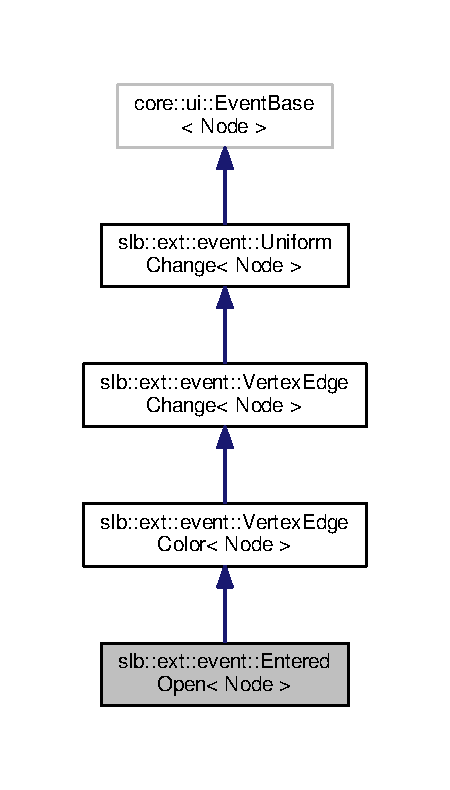
\includegraphics[width=216pt]{structslb_1_1ext_1_1event_1_1EnteredOpen__inherit__graph}
\end{center}
\end{figure}


Collaboration diagram for slb\+:\+:ext\+:\+:event\+:\+:Entered\+Open$<$ Node $>$\+:\nopagebreak
\begin{figure}[H]
\begin{center}
\leavevmode
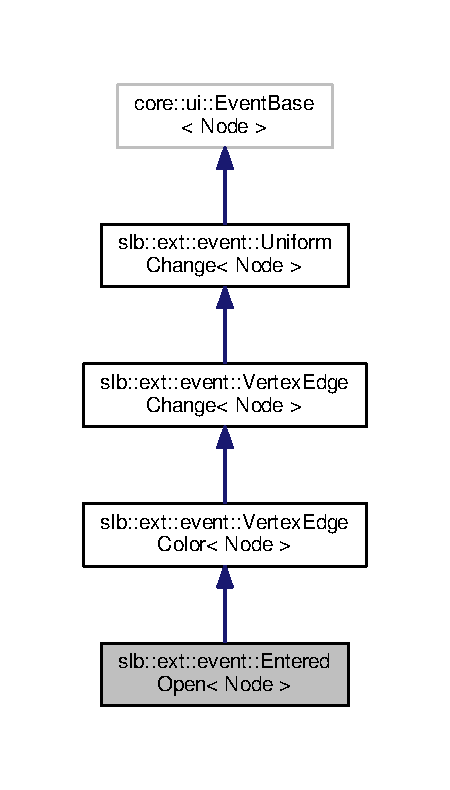
\includegraphics[width=216pt]{structslb_1_1ext_1_1event_1_1EnteredOpen__coll__graph}
\end{center}
\end{figure}
\subsubsection*{Private Member Functions}
\begin{DoxyCompactItemize}
\item 
virtual Color \hyperlink{structslb_1_1ext_1_1event_1_1EnteredOpen_ae9d3efea90ef2050c58f5744ade0d645}{color} () const override
\begin{DoxyCompactList}\small\item\em Returns the new color of both the vertex of the state graph corresponding to the state associated with the event and the edge by which the search algorithm arrived to this state. \end{DoxyCompactList}\item 
std\+::string \hyperlink{structslb_1_1ext_1_1event_1_1EnteredOpen_acd82f78256006e52aa541106c6a0c31f}{event\+Str} () const override
\begin{DoxyCompactList}\small\item\em Returns the string describing the event. This string is displayed in the log window. \end{DoxyCompactList}\end{DoxyCompactItemize}
\subsubsection*{Additional Inherited Members}


\subsubsection{Detailed Description}
\subsubsection*{template$<$class Node = S\+L\+B\+\_\+\+N\+O\+DE$>$\\*
struct slb\+::ext\+::event\+::\+Entered\+Open$<$ Node $>$}

Event that visualizes a node entering the Open List. 


\begin{DoxyTemplParams}{Template Parameters}
{\em Node} & The search node type. \\
\hline
\end{DoxyTemplParams}


Definition at line 138 of file events.\+h.



\subsubsection{Member Function Documentation}
\index{slb\+::ext\+::event\+::\+Entered\+Open@{slb\+::ext\+::event\+::\+Entered\+Open}!color@{color}}
\index{color@{color}!slb\+::ext\+::event\+::\+Entered\+Open@{slb\+::ext\+::event\+::\+Entered\+Open}}
\paragraph[{\texorpdfstring{color() const override}{color() const override}}]{\setlength{\rightskip}{0pt plus 5cm}template$<$class Node  = S\+L\+B\+\_\+\+N\+O\+DE$>$ virtual Color {\bf slb\+::ext\+::event\+::\+Entered\+Open}$<$ Node $>$\+::color (
\begin{DoxyParamCaption}
{}
\end{DoxyParamCaption}
) const\hspace{0.3cm}{\ttfamily [inline]}, {\ttfamily [override]}, {\ttfamily [private]}, {\ttfamily [virtual]}}\hypertarget{structslb_1_1ext_1_1event_1_1EnteredOpen_ae9d3efea90ef2050c58f5744ade0d645}{}\label{structslb_1_1ext_1_1event_1_1EnteredOpen_ae9d3efea90ef2050c58f5744ade0d645}


Returns the new color of both the vertex of the state graph corresponding to the state associated with the event and the edge by which the search algorithm arrived to this state. 

\begin{DoxyReturn}{Returns}
The new color of both the vertex of the state graph corresponding to the state associated with the event and the edge by which the search algorithm arrived to this state. 
\end{DoxyReturn}


Implements \hyperlink{structslb_1_1ext_1_1event_1_1VertexEdgeColor_ac5d0c212a4e807eccbc7082b8834ef77}{slb\+::ext\+::event\+::\+Vertex\+Edge\+Color$<$ Node $>$}.



Definition at line 149 of file events.\+h.

\index{slb\+::ext\+::event\+::\+Entered\+Open@{slb\+::ext\+::event\+::\+Entered\+Open}!event\+Str@{event\+Str}}
\index{event\+Str@{event\+Str}!slb\+::ext\+::event\+::\+Entered\+Open@{slb\+::ext\+::event\+::\+Entered\+Open}}
\paragraph[{\texorpdfstring{event\+Str() const override}{eventStr() const override}}]{\setlength{\rightskip}{0pt plus 5cm}template$<$class Node  = S\+L\+B\+\_\+\+N\+O\+DE$>$ std\+::string {\bf slb\+::ext\+::event\+::\+Entered\+Open}$<$ Node $>$\+::event\+Str (
\begin{DoxyParamCaption}
{}
\end{DoxyParamCaption}
) const\hspace{0.3cm}{\ttfamily [inline]}, {\ttfamily [override]}, {\ttfamily [private]}}\hypertarget{structslb_1_1ext_1_1event_1_1EnteredOpen_acd82f78256006e52aa541106c6a0c31f}{}\label{structslb_1_1ext_1_1event_1_1EnteredOpen_acd82f78256006e52aa541106c6a0c31f}


Returns the string describing the event. This string is displayed in the log window. 

\begin{DoxyReturn}{Returns}
The string describing the event. 
\end{DoxyReturn}


Definition at line 154 of file events.\+h.



The documentation for this struct was generated from the following file\+:\begin{DoxyCompactItemize}
\item 
extensions/events/\hyperlink{events_8h}{events.\+h}\end{DoxyCompactItemize}

\hypertarget{structslb_1_1core_1_1ui_1_1EventBase}{}\subsection{slb\+:\+:core\+:\+:ui\+:\+:Event\+Base$<$ Node $>$ Struct Template Reference}
\label{structslb_1_1core_1_1ui_1_1EventBase}\index{slb\+::core\+::ui\+::\+Event\+Base$<$ Node $>$@{slb\+::core\+::ui\+::\+Event\+Base$<$ Node $>$}}


The base class for the events generated by the search algorithm. Note that an event carries with it the information about its visualization as well. This information is the basis for building a visual event (\hyperlink{structslb_1_1core_1_1ui_1_1VisualEvent}{Visual\+Event}) out of it.  




{\ttfamily \#include $<$event\+\_\+base.\+h$>$}



Collaboration diagram for slb\+:\+:core\+:\+:ui\+:\+:Event\+Base$<$ Node $>$\+:\nopagebreak
\begin{figure}[H]
\begin{center}
\leavevmode
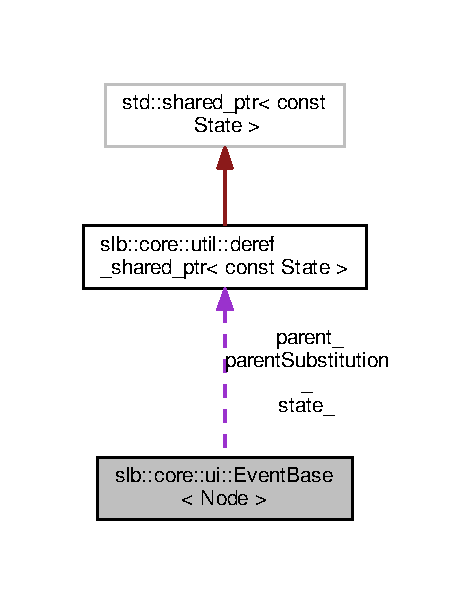
\includegraphics[width=227pt]{structslb_1_1core_1_1ui_1_1EventBase__coll__graph}
\end{center}
\end{figure}
\subsubsection*{Classes}
\begin{DoxyCompactItemize}
\item 
struct \hyperlink{structslb_1_1core_1_1ui_1_1EventBase_1_1EdgeChange}{Edge\+Change}
\begin{DoxyCompactList}\small\item\em Description of change of visual representation of an edge. An edge is represented here by a pair of smart pointers to states. Note that this is different from a visual event (see \hyperlink{structslb_1_1core_1_1ui_1_1VisualEvent_1_1EdgeChange}{Visual\+Event\+::\+Edge\+Change}), in which an edge is represented here by a pair of vertices of the domain graph. \end{DoxyCompactList}\item 
struct \hyperlink{structslb_1_1core_1_1ui_1_1EventBase_1_1VertexChange}{Vertex\+Change}
\begin{DoxyCompactList}\small\item\em Description of change of visual representation a state. Note that this is different from a visual event (see \hyperlink{structslb_1_1core_1_1ui_1_1VisualEvent_1_1VertexChange}{Visual\+Event\+::\+Vertex\+Change}), which associates changes with vertices of the domain graph. \end{DoxyCompactList}\item 
struct \hyperlink{structslb_1_1core_1_1ui_1_1EventBase_1_1VisualChanges}{Visual\+Changes}
\begin{DoxyCompactList}\small\item\em Changes of visual representations associated with states and edges. \end{DoxyCompactList}\end{DoxyCompactItemize}
\subsubsection*{Public Types}
\begin{DoxyCompactItemize}
\item 
using \hyperlink{structslb_1_1core_1_1ui_1_1EventBase_a2fe332d7f0fa68fe45a0b2e31c6790d1}{State} = typename Node\+::\+State\hypertarget{structslb_1_1core_1_1ui_1_1EventBase_a2fe332d7f0fa68fe45a0b2e31c6790d1}{}\label{structslb_1_1core_1_1ui_1_1EventBase_a2fe332d7f0fa68fe45a0b2e31c6790d1}

\begin{DoxyCompactList}\small\item\em The state type, represents the domain. \end{DoxyCompactList}\item 
using \hyperlink{structslb_1_1core_1_1ui_1_1EventBase_a50419d00607aad434bb97138eabe2c94}{State\+Shared\+Ptr} = \hyperlink{classslb_1_1core_1_1util_1_1deref__shared__ptr}{deref\+\_\+shared\+\_\+ptr}$<$ const \hyperlink{structslb_1_1core_1_1ui_1_1EventBase_a2fe332d7f0fa68fe45a0b2e31c6790d1}{State} $>$\hypertarget{structslb_1_1core_1_1ui_1_1EventBase_a50419d00607aad434bb97138eabe2c94}{}\label{structslb_1_1core_1_1ui_1_1EventBase_a50419d00607aad434bb97138eabe2c94}

\begin{DoxyCompactList}\small\item\em Smart pointer to state. \end{DoxyCompactList}\item 
using \hyperlink{structslb_1_1core_1_1ui_1_1EventBase_a1eefdf6331e2af79cd1ba37eff880a18}{Node\+Data} = typename Node\+::\+Node\+Data\hypertarget{structslb_1_1core_1_1ui_1_1EventBase_a1eefdf6331e2af79cd1ba37eff880a18}{}\label{structslb_1_1core_1_1ui_1_1EventBase_a1eefdf6331e2af79cd1ba37eff880a18}

\begin{DoxyCompactList}\small\item\em Type for data carried with a node. \end{DoxyCompactList}\item 
using \hyperlink{structslb_1_1core_1_1ui_1_1EventBase_a7b61ed0ba0f2fdeb854c631188725d37}{Event} = std\+::shared\+\_\+ptr$<$ \hyperlink{structslb_1_1core_1_1ui_1_1EventBase}{Event\+Base}$<$ Node $>$$>$\hypertarget{structslb_1_1core_1_1ui_1_1EventBase_a7b61ed0ba0f2fdeb854c631188725d37}{}\label{structslb_1_1core_1_1ui_1_1EventBase_a7b61ed0ba0f2fdeb854c631188725d37}

\begin{DoxyCompactList}\small\item\em Smart pointer to an event generated by the search algorithm. \end{DoxyCompactList}\end{DoxyCompactItemize}
\subsubsection*{Public Member Functions}
\begin{DoxyCompactItemize}
\item 
\hyperlink{structslb_1_1core_1_1ui_1_1EventBase_a641bed2ef08022f532763268aac71e3a}{Event\+Base} (const \hyperlink{structslb_1_1core_1_1ui_1_1AlgorithmLog}{Algorithm\+Log}$<$ Node $>$ \&\hyperlink{structslb_1_1core_1_1ui_1_1EventBase_a4f6cd3f19f35b8e9dd39aa1a141be99f}{log}, const Node $\ast$n, const Node $\ast$parent\+Substitution=nullptr)
\begin{DoxyCompactList}\small\item\em Initializes the event based on the given search node. \end{DoxyCompactList}\item 
int \hyperlink{structslb_1_1core_1_1ui_1_1EventBase_a23ec95b8b30e74fe830f5bd60d93ed75}{step} () const 
\begin{DoxyCompactList}\small\item\em Returns the time point when the event happened. \end{DoxyCompactList}\item 
const \hyperlink{structslb_1_1core_1_1ui_1_1AlgorithmLog}{Algorithm\+Log}$<$ Node $>$ \& \hyperlink{structslb_1_1core_1_1ui_1_1EventBase_a4f6cd3f19f35b8e9dd39aa1a141be99f}{log} () const 
\begin{DoxyCompactList}\small\item\em Returns the log containing the event. \end{DoxyCompactList}\item 
const \hyperlink{structslb_1_1core_1_1ui_1_1EventBase_a50419d00607aad434bb97138eabe2c94}{State\+Shared\+Ptr} \& \hyperlink{structslb_1_1core_1_1ui_1_1EventBase_a1890daf7f5d663402d2272ba5f41f4d7}{state} () const 
\begin{DoxyCompactList}\small\item\em Returns the state with which the event is associated. \end{DoxyCompactList}\item 
const \hyperlink{structslb_1_1core_1_1ui_1_1EventBase_a50419d00607aad434bb97138eabe2c94}{State\+Shared\+Ptr} \& \hyperlink{structslb_1_1core_1_1ui_1_1EventBase_a9de09dd2012486bbf7a486b12c161ec2}{parent} () const 
\begin{DoxyCompactList}\small\item\em Returns the state from which the search algorithm arrived to the state with which the event is associated. \end{DoxyCompactList}\item 
const \hyperlink{structslb_1_1core_1_1ui_1_1EventBase_a1eefdf6331e2af79cd1ba37eff880a18}{Node\+Data} \& \hyperlink{structslb_1_1core_1_1ui_1_1EventBase_a6ea3aa8fc149f08ff986076852d7802b}{node\+Data} () const 
\begin{DoxyCompactList}\small\item\em Returns the information kept with the search node from which the event was constructed. \end{DoxyCompactList}\item 
\hyperlink{structslb_1_1core_1_1ui_1_1EventBase_a7b61ed0ba0f2fdeb854c631188725d37}{Event} \hyperlink{structslb_1_1core_1_1ui_1_1EventBase_af3b3faf8b00ae20b921bd12a21e865d1}{last\+State\+Event} () const 
\begin{DoxyCompactList}\small\item\em Returns latest among the past events for the state. \end{DoxyCompactList}\item 
\hyperlink{structslb_1_1core_1_1ui_1_1EventBase_a7b61ed0ba0f2fdeb854c631188725d37}{Event} \hyperlink{structslb_1_1core_1_1ui_1_1EventBase_a5cc22688f532de0e32a50bbe3188f17a}{last\+Parent\+Event} () const 
\begin{DoxyCompactList}\small\item\em Returns latest among the past events for the parent state. \end{DoxyCompactList}\item 
virtual std\+::string \hyperlink{structslb_1_1core_1_1ui_1_1EventBase_a048e92286f3ee57db7e9447b5bd192ba}{event\+Str} () const =0
\begin{DoxyCompactList}\small\item\em Returns the string describing the event. This string is displayed in the log window. \end{DoxyCompactList}\item 
virtual \hyperlink{namespaceslb_1_1core_1_1ui_ae44f7078122b3f63928fd619fadd2dcd}{Event\+Type} \hyperlink{structslb_1_1core_1_1ui_1_1EventBase_ac9767dc972acabf2c250fd4dd30a5081}{event\+Type} () const 
\begin{DoxyCompactList}\small\item\em Returns the event type (see \hyperlink{namespaceslb_1_1core_1_1ui_ae44f7078122b3f63928fd619fadd2dcd}{Event\+Type}). \end{DoxyCompactList}\item 
std\+::vector$<$ \hyperlink{structslb_1_1core_1_1ui_1_1EventBase_a50419d00607aad434bb97138eabe2c94}{State\+Shared\+Ptr} $>$ \hyperlink{structslb_1_1core_1_1ui_1_1EventBase_ae324be109b4869e5c3e85f950ef83ff1}{path} (const \hyperlink{structslb_1_1core_1_1ui_1_1EventBase_a50419d00607aad434bb97138eabe2c94}{State\+Shared\+Ptr} \&\hyperlink{structslb_1_1core_1_1ui_1_1EventBase_a1890daf7f5d663402d2272ba5f41f4d7}{state}) const 
\begin{DoxyCompactList}\small\item\em Uses the log to compute the path which the search algorithm found to arrive to the given state. \end{DoxyCompactList}\item 
virtual \hyperlink{structslb_1_1core_1_1ui_1_1EventBase_1_1VisualChanges}{Visual\+Changes} \hyperlink{structslb_1_1core_1_1ui_1_1EventBase_aa69b46193dcce78ad18003ca0c222566}{visual\+Changes} (const \hyperlink{structslb_1_1core_1_1ui_1_1CurrentStyles}{Current\+Styles}$<$ \hyperlink{structslb_1_1core_1_1ui_1_1EventBase_a2fe332d7f0fa68fe45a0b2e31c6790d1}{State} $>$ \&styles) const 
\begin{DoxyCompactList}\small\item\em Computes changes of visual representations associated with states and edges defined by the event. \end{DoxyCompactList}\item 
{\footnotesize template$<$class Stream $>$ }\\Stream \& \hyperlink{structslb_1_1core_1_1ui_1_1EventBase_a7c66eba76be0fb26ae508e04dd269f9c}{dump} (Stream \&o) const 
\begin{DoxyCompactList}\small\item\em Dumps the event into a given output stream in column format. The stream will usually be a \hyperlink{structslb_1_1core_1_1util_1_1Table}{util\+::\+Table}, which handles the column width automatically. \end{DoxyCompactList}\end{DoxyCompactItemize}
\subsubsection*{Static Public Member Functions}
\begin{DoxyCompactItemize}
\item 
{\footnotesize template$<$class Stream $>$ }\\static Stream \& \hyperlink{structslb_1_1core_1_1ui_1_1EventBase_af03180ec147799c8efd1eee5f747a583}{dump\+Title} (Stream \&o)
\begin{DoxyCompactList}\small\item\em To be used in conjunction with \hyperlink{structslb_1_1core_1_1ui_1_1EventBase_a7c66eba76be0fb26ae508e04dd269f9c}{dump}. Dumps the titles of the columns. \end{DoxyCompactList}\end{DoxyCompactItemize}
\subsubsection*{Protected Attributes}
\begin{DoxyCompactItemize}
\item 
const \hyperlink{structslb_1_1core_1_1ui_1_1AlgorithmLog}{Algorithm\+Log}$<$ Node $>$ \& \hyperlink{structslb_1_1core_1_1ui_1_1EventBase_a188bf6c9b61aece44727bee80c0f284c}{log\+\_\+}\hypertarget{structslb_1_1core_1_1ui_1_1EventBase_a188bf6c9b61aece44727bee80c0f284c}{}\label{structslb_1_1core_1_1ui_1_1EventBase_a188bf6c9b61aece44727bee80c0f284c}

\begin{DoxyCompactList}\small\item\em The log containing the event. \end{DoxyCompactList}\item 
\hyperlink{structslb_1_1core_1_1ui_1_1EventBase_a50419d00607aad434bb97138eabe2c94}{State\+Shared\+Ptr} \hyperlink{structslb_1_1core_1_1ui_1_1EventBase_afdac9dcd9ab7162d0ae87f7b414ae9cb}{state\+\_\+}\hypertarget{structslb_1_1core_1_1ui_1_1EventBase_afdac9dcd9ab7162d0ae87f7b414ae9cb}{}\label{structslb_1_1core_1_1ui_1_1EventBase_afdac9dcd9ab7162d0ae87f7b414ae9cb}

\begin{DoxyCompactList}\small\item\em The state with which the event is associated. \end{DoxyCompactList}\item 
\hyperlink{structslb_1_1core_1_1ui_1_1EventBase_a50419d00607aad434bb97138eabe2c94}{State\+Shared\+Ptr} \hyperlink{structslb_1_1core_1_1ui_1_1EventBase_a6753a8d0750fee732416533768c7b532}{parent\+\_\+}\hypertarget{structslb_1_1core_1_1ui_1_1EventBase_a6753a8d0750fee732416533768c7b532}{}\label{structslb_1_1core_1_1ui_1_1EventBase_a6753a8d0750fee732416533768c7b532}

\begin{DoxyCompactList}\small\item\em the state from which the search algorithm arrived to \hyperlink{structslb_1_1core_1_1ui_1_1EventBase_afdac9dcd9ab7162d0ae87f7b414ae9cb}{state\+\_\+}. \end{DoxyCompactList}\item 
\hyperlink{structslb_1_1core_1_1ui_1_1EventBase_a50419d00607aad434bb97138eabe2c94}{State\+Shared\+Ptr} \hyperlink{structslb_1_1core_1_1ui_1_1EventBase_a24499f337e544dc299bdc7756d4c365c}{parent\+Substitution\+\_\+}\hypertarget{structslb_1_1core_1_1ui_1_1EventBase_a24499f337e544dc299bdc7756d4c365c}{}\label{structslb_1_1core_1_1ui_1_1EventBase_a24499f337e544dc299bdc7756d4c365c}

\begin{DoxyCompactList}\small\item\em The node whose state should be used as a parent state instead of the parent stored in ~\newline
. See how the \hyperlink{structslb_1_1ext_1_1event_1_1NothingToDo}{ext\+::event\+::\+Nothing\+To\+Do} event is generated in \hyperlink{structslb_1_1ext_1_1algorithm_1_1Astar}{ext\+::algorithm\+::\+Astar} for an example of when this is useful. \end{DoxyCompactList}\item 
\hyperlink{structslb_1_1core_1_1ui_1_1EventBase_a1eefdf6331e2af79cd1ba37eff880a18}{Node\+Data} \hyperlink{structslb_1_1core_1_1ui_1_1EventBase_af94e406ffc21c85314b3ef4379ed40da}{node\+Data\+\_\+}\hypertarget{structslb_1_1core_1_1ui_1_1EventBase_af94e406ffc21c85314b3ef4379ed40da}{}\label{structslb_1_1core_1_1ui_1_1EventBase_af94e406ffc21c85314b3ef4379ed40da}

\begin{DoxyCompactList}\small\item\em The information that was kept with the search node from which the event was constructed at the moment of construction. \end{DoxyCompactList}\item 
int \hyperlink{structslb_1_1core_1_1ui_1_1EventBase_a8a22e5faef2804761d29accd8174d4f9}{step\+\_\+}\hypertarget{structslb_1_1core_1_1ui_1_1EventBase_a8a22e5faef2804761d29accd8174d4f9}{}\label{structslb_1_1core_1_1ui_1_1EventBase_a8a22e5faef2804761d29accd8174d4f9}

\begin{DoxyCompactList}\small\item\em The time point when the event happened. \end{DoxyCompactList}\item 
\hyperlink{structslb_1_1core_1_1ui_1_1EventBase_a7b61ed0ba0f2fdeb854c631188725d37}{Event} \hyperlink{structslb_1_1core_1_1ui_1_1EventBase_a54f145d471419194b65eaa0de024d7ac}{last\+State\+Event\+\_\+}\hypertarget{structslb_1_1core_1_1ui_1_1EventBase_a54f145d471419194b65eaa0de024d7ac}{}\label{structslb_1_1core_1_1ui_1_1EventBase_a54f145d471419194b65eaa0de024d7ac}

\begin{DoxyCompactList}\small\item\em The latest among the past events for the state. \end{DoxyCompactList}\item 
\hyperlink{structslb_1_1core_1_1ui_1_1EventBase_a7b61ed0ba0f2fdeb854c631188725d37}{Event} \hyperlink{structslb_1_1core_1_1ui_1_1EventBase_af19c67b003d90e40b84b8bed395a3662}{last\+Parent\+Event\+\_\+}\hypertarget{structslb_1_1core_1_1ui_1_1EventBase_af19c67b003d90e40b84b8bed395a3662}{}\label{structslb_1_1core_1_1ui_1_1EventBase_af19c67b003d90e40b84b8bed395a3662}

\begin{DoxyCompactList}\small\item\em The latest among the past events for the parent state. \end{DoxyCompactList}\end{DoxyCompactItemize}
\subsubsection*{Private Member Functions}
\begin{DoxyCompactItemize}
\item 
\hyperlink{structslb_1_1core_1_1ui_1_1EventBase_a50419d00607aad434bb97138eabe2c94}{State\+Shared\+Ptr} \hyperlink{structslb_1_1core_1_1ui_1_1EventBase_ad4b4485000eba6045376fc3ca55ac2ac}{state\+From\+Node} (const Node $\ast$n)
\begin{DoxyCompactList}\small\item\em Get a smart pointer to the state stored with the given search node. n The search node. \end{DoxyCompactList}\end{DoxyCompactItemize}


\subsubsection{Detailed Description}
\subsubsection*{template$<$class Node = S\+L\+B\+\_\+\+N\+O\+DE$>$\\*
struct slb\+::core\+::ui\+::\+Event\+Base$<$ Node $>$}

The base class for the events generated by the search algorithm. Note that an event carries with it the information about its visualization as well. This information is the basis for building a visual event (\hyperlink{structslb_1_1core_1_1ui_1_1VisualEvent}{Visual\+Event}) out of it. 


\begin{DoxyTemplParams}{Template Parameters}
{\em Node} & The node type. An event usually carries data from a search node. This data is used to display the event in the log window. \\
\hline
\end{DoxyTemplParams}


Definition at line 14 of file algorithm\+\_\+log.\+h.



\subsubsection{Constructor \& Destructor Documentation}
\index{slb\+::core\+::ui\+::\+Event\+Base@{slb\+::core\+::ui\+::\+Event\+Base}!Event\+Base@{Event\+Base}}
\index{Event\+Base@{Event\+Base}!slb\+::core\+::ui\+::\+Event\+Base@{slb\+::core\+::ui\+::\+Event\+Base}}
\paragraph[{\texorpdfstring{Event\+Base(const Algorithm\+Log$<$ Node $>$ \&log, const Node $\ast$n, const Node $\ast$parent\+Substitution=nullptr)}{EventBase(const AlgorithmLog< Node > &log, const Node *n, const Node *parentSubstitution=nullptr)}}]{\setlength{\rightskip}{0pt plus 5cm}template$<$class Node  = S\+L\+B\+\_\+\+N\+O\+DE$>$ {\bf slb\+::core\+::ui\+::\+Event\+Base}$<$ Node $>$\+::{\bf Event\+Base} (
\begin{DoxyParamCaption}
\item[{const {\bf Algorithm\+Log}$<$ Node $>$ \&}]{log, }
\item[{const Node $\ast$}]{n, }
\item[{const Node $\ast$}]{parent\+Substitution = {\ttfamily nullptr}}
\end{DoxyParamCaption}
)\hspace{0.3cm}{\ttfamily [inline]}}\hypertarget{structslb_1_1core_1_1ui_1_1EventBase_a641bed2ef08022f532763268aac71e3a}{}\label{structslb_1_1core_1_1ui_1_1EventBase_a641bed2ef08022f532763268aac71e3a}


Initializes the event based on the given search node. 


\begin{DoxyParams}{Parameters}
{\em log} & The log that contains the event. This means that the log is an intrusive container. See \hyperlink{structslb_1_1core_1_1ui_1_1AlgorithmLog}{Algorithm\+Log}. \\
\hline
{\em n} & The node. \\
\hline
{\em parent\+Substitution} & The node whose state should be used as a parent state instead of the parent stored in ~\newline
. See How the \hyperlink{structslb_1_1ext_1_1event_1_1NothingToDo}{ext\+::event\+::\+Nothing\+To\+Do} event is generated in \hyperlink{structslb_1_1ext_1_1algorithm_1_1Astar}{ext\+::algorithm\+::\+Astar} for an example of when this is useful. \\
\hline
\end{DoxyParams}


Definition at line 79 of file event\+\_\+base.\+h.



\subsubsection{Member Function Documentation}
\index{slb\+::core\+::ui\+::\+Event\+Base@{slb\+::core\+::ui\+::\+Event\+Base}!dump@{dump}}
\index{dump@{dump}!slb\+::core\+::ui\+::\+Event\+Base@{slb\+::core\+::ui\+::\+Event\+Base}}
\paragraph[{\texorpdfstring{dump(\+Stream \&o) const }{dump(Stream &o) const }}]{\setlength{\rightskip}{0pt plus 5cm}template$<$class Node  = S\+L\+B\+\_\+\+N\+O\+DE$>$ template$<$class Stream $>$ Stream\& {\bf slb\+::core\+::ui\+::\+Event\+Base}$<$ Node $>$\+::dump (
\begin{DoxyParamCaption}
\item[{Stream \&}]{o}
\end{DoxyParamCaption}
) const\hspace{0.3cm}{\ttfamily [inline]}}\hypertarget{structslb_1_1core_1_1ui_1_1EventBase_a7c66eba76be0fb26ae508e04dd269f9c}{}\label{structslb_1_1core_1_1ui_1_1EventBase_a7c66eba76be0fb26ae508e04dd269f9c}


Dumps the event into a given output stream in column format. The stream will usually be a \hyperlink{structslb_1_1core_1_1util_1_1Table}{util\+::\+Table}, which handles the column width automatically. 


\begin{DoxyTemplParams}{Template Parameters}
{\em Stream} & The output stream type. \\
\hline
\end{DoxyTemplParams}

\begin{DoxyParams}{Parameters}
{\em o} & The output stream. \\
\hline
\end{DoxyParams}


Definition at line 165 of file event\+\_\+base.\+h.

\index{slb\+::core\+::ui\+::\+Event\+Base@{slb\+::core\+::ui\+::\+Event\+Base}!dump\+Title@{dump\+Title}}
\index{dump\+Title@{dump\+Title}!slb\+::core\+::ui\+::\+Event\+Base@{slb\+::core\+::ui\+::\+Event\+Base}}
\paragraph[{\texorpdfstring{dump\+Title(\+Stream \&o)}{dumpTitle(Stream &o)}}]{\setlength{\rightskip}{0pt plus 5cm}template$<$class Node  = S\+L\+B\+\_\+\+N\+O\+DE$>$ template$<$class Stream $>$ static Stream\& {\bf slb\+::core\+::ui\+::\+Event\+Base}$<$ Node $>$\+::dump\+Title (
\begin{DoxyParamCaption}
\item[{Stream \&}]{o}
\end{DoxyParamCaption}
)\hspace{0.3cm}{\ttfamily [inline]}, {\ttfamily [static]}}\hypertarget{structslb_1_1core_1_1ui_1_1EventBase_af03180ec147799c8efd1eee5f747a583}{}\label{structslb_1_1core_1_1ui_1_1EventBase_af03180ec147799c8efd1eee5f747a583}


To be used in conjunction with \hyperlink{structslb_1_1core_1_1ui_1_1EventBase_a7c66eba76be0fb26ae508e04dd269f9c}{dump}. Dumps the titles of the columns. 


\begin{DoxyTemplParams}{Template Parameters}
{\em Stream} & The output stream type. \\
\hline
\end{DoxyTemplParams}

\begin{DoxyParams}{Parameters}
{\em o} & The output stream. \\
\hline
\end{DoxyParams}


Definition at line 191 of file event\+\_\+base.\+h.

\index{slb\+::core\+::ui\+::\+Event\+Base@{slb\+::core\+::ui\+::\+Event\+Base}!event\+Str@{event\+Str}}
\index{event\+Str@{event\+Str}!slb\+::core\+::ui\+::\+Event\+Base@{slb\+::core\+::ui\+::\+Event\+Base}}
\paragraph[{\texorpdfstring{event\+Str() const =0}{eventStr() const =0}}]{\setlength{\rightskip}{0pt plus 5cm}template$<$class Node  = S\+L\+B\+\_\+\+N\+O\+DE$>$ virtual std\+::string {\bf slb\+::core\+::ui\+::\+Event\+Base}$<$ Node $>$\+::event\+Str (
\begin{DoxyParamCaption}
{}
\end{DoxyParamCaption}
) const\hspace{0.3cm}{\ttfamily [pure virtual]}}\hypertarget{structslb_1_1core_1_1ui_1_1EventBase_a048e92286f3ee57db7e9447b5bd192ba}{}\label{structslb_1_1core_1_1ui_1_1EventBase_a048e92286f3ee57db7e9447b5bd192ba}


Returns the string describing the event. This string is displayed in the log window. 

\begin{DoxyReturn}{Returns}
The string describing the event. 
\end{DoxyReturn}
\index{slb\+::core\+::ui\+::\+Event\+Base@{slb\+::core\+::ui\+::\+Event\+Base}!event\+Type@{event\+Type}}
\index{event\+Type@{event\+Type}!slb\+::core\+::ui\+::\+Event\+Base@{slb\+::core\+::ui\+::\+Event\+Base}}
\paragraph[{\texorpdfstring{event\+Type() const }{eventType() const }}]{\setlength{\rightskip}{0pt plus 5cm}template$<$class Node  = S\+L\+B\+\_\+\+N\+O\+DE$>$ virtual {\bf Event\+Type} {\bf slb\+::core\+::ui\+::\+Event\+Base}$<$ Node $>$\+::event\+Type (
\begin{DoxyParamCaption}
{}
\end{DoxyParamCaption}
) const\hspace{0.3cm}{\ttfamily [inline]}, {\ttfamily [virtual]}}\hypertarget{structslb_1_1core_1_1ui_1_1EventBase_ac9767dc972acabf2c250fd4dd30a5081}{}\label{structslb_1_1core_1_1ui_1_1EventBase_ac9767dc972acabf2c250fd4dd30a5081}


Returns the event type (see \hyperlink{namespaceslb_1_1core_1_1ui_ae44f7078122b3f63928fd619fadd2dcd}{Event\+Type}). 

\begin{DoxyReturn}{Returns}
The event type. 
\end{DoxyReturn}


Definition at line 130 of file event\+\_\+base.\+h.

\index{slb\+::core\+::ui\+::\+Event\+Base@{slb\+::core\+::ui\+::\+Event\+Base}!last\+Parent\+Event@{last\+Parent\+Event}}
\index{last\+Parent\+Event@{last\+Parent\+Event}!slb\+::core\+::ui\+::\+Event\+Base@{slb\+::core\+::ui\+::\+Event\+Base}}
\paragraph[{\texorpdfstring{last\+Parent\+Event() const }{lastParentEvent() const }}]{\setlength{\rightskip}{0pt plus 5cm}template$<$class Node  = S\+L\+B\+\_\+\+N\+O\+DE$>$ {\bf Event} {\bf slb\+::core\+::ui\+::\+Event\+Base}$<$ Node $>$\+::last\+Parent\+Event (
\begin{DoxyParamCaption}
{}
\end{DoxyParamCaption}
) const\hspace{0.3cm}{\ttfamily [inline]}}\hypertarget{structslb_1_1core_1_1ui_1_1EventBase_a5cc22688f532de0e32a50bbe3188f17a}{}\label{structslb_1_1core_1_1ui_1_1EventBase_a5cc22688f532de0e32a50bbe3188f17a}


Returns latest among the past events for the parent state. 

\begin{DoxyReturn}{Returns}
Smart pointer to the latest among the past events for the parent state. 
\end{DoxyReturn}


Definition at line 121 of file event\+\_\+base.\+h.

\index{slb\+::core\+::ui\+::\+Event\+Base@{slb\+::core\+::ui\+::\+Event\+Base}!last\+State\+Event@{last\+State\+Event}}
\index{last\+State\+Event@{last\+State\+Event}!slb\+::core\+::ui\+::\+Event\+Base@{slb\+::core\+::ui\+::\+Event\+Base}}
\paragraph[{\texorpdfstring{last\+State\+Event() const }{lastStateEvent() const }}]{\setlength{\rightskip}{0pt plus 5cm}template$<$class Node  = S\+L\+B\+\_\+\+N\+O\+DE$>$ {\bf Event} {\bf slb\+::core\+::ui\+::\+Event\+Base}$<$ Node $>$\+::last\+State\+Event (
\begin{DoxyParamCaption}
{}
\end{DoxyParamCaption}
) const\hspace{0.3cm}{\ttfamily [inline]}}\hypertarget{structslb_1_1core_1_1ui_1_1EventBase_af3b3faf8b00ae20b921bd12a21e865d1}{}\label{structslb_1_1core_1_1ui_1_1EventBase_af3b3faf8b00ae20b921bd12a21e865d1}


Returns latest among the past events for the state. 

\begin{DoxyReturn}{Returns}
Smart pointer to the latest among the past events for the state. 
\end{DoxyReturn}


Definition at line 116 of file event\+\_\+base.\+h.

\index{slb\+::core\+::ui\+::\+Event\+Base@{slb\+::core\+::ui\+::\+Event\+Base}!log@{log}}
\index{log@{log}!slb\+::core\+::ui\+::\+Event\+Base@{slb\+::core\+::ui\+::\+Event\+Base}}
\paragraph[{\texorpdfstring{log() const }{log() const }}]{\setlength{\rightskip}{0pt plus 5cm}template$<$class Node  = S\+L\+B\+\_\+\+N\+O\+DE$>$ const {\bf Algorithm\+Log}$<$Node$>$\& {\bf slb\+::core\+::ui\+::\+Event\+Base}$<$ Node $>$\+::log (
\begin{DoxyParamCaption}
{}
\end{DoxyParamCaption}
) const\hspace{0.3cm}{\ttfamily [inline]}}\hypertarget{structslb_1_1core_1_1ui_1_1EventBase_a4f6cd3f19f35b8e9dd39aa1a141be99f}{}\label{structslb_1_1core_1_1ui_1_1EventBase_a4f6cd3f19f35b8e9dd39aa1a141be99f}


Returns the log containing the event. 

\begin{DoxyReturn}{Returns}
Const reference to the log containing the event. 
\end{DoxyReturn}


Definition at line 97 of file event\+\_\+base.\+h.

\index{slb\+::core\+::ui\+::\+Event\+Base@{slb\+::core\+::ui\+::\+Event\+Base}!node\+Data@{node\+Data}}
\index{node\+Data@{node\+Data}!slb\+::core\+::ui\+::\+Event\+Base@{slb\+::core\+::ui\+::\+Event\+Base}}
\paragraph[{\texorpdfstring{node\+Data() const }{nodeData() const }}]{\setlength{\rightskip}{0pt plus 5cm}template$<$class Node  = S\+L\+B\+\_\+\+N\+O\+DE$>$ const {\bf Node\+Data}\& {\bf slb\+::core\+::ui\+::\+Event\+Base}$<$ Node $>$\+::node\+Data (
\begin{DoxyParamCaption}
{}
\end{DoxyParamCaption}
) const\hspace{0.3cm}{\ttfamily [inline]}}\hypertarget{structslb_1_1core_1_1ui_1_1EventBase_a6ea3aa8fc149f08ff986076852d7802b}{}\label{structslb_1_1core_1_1ui_1_1EventBase_a6ea3aa8fc149f08ff986076852d7802b}


Returns the information kept with the search node from which the event was constructed. 

\begin{DoxyReturn}{Returns}
Const reference to the structure with the information kept with the search node, from which the event was constructed.. 
\end{DoxyReturn}


Definition at line 112 of file event\+\_\+base.\+h.

\index{slb\+::core\+::ui\+::\+Event\+Base@{slb\+::core\+::ui\+::\+Event\+Base}!parent@{parent}}
\index{parent@{parent}!slb\+::core\+::ui\+::\+Event\+Base@{slb\+::core\+::ui\+::\+Event\+Base}}
\paragraph[{\texorpdfstring{parent() const }{parent() const }}]{\setlength{\rightskip}{0pt plus 5cm}template$<$class Node  = S\+L\+B\+\_\+\+N\+O\+DE$>$ const {\bf State\+Shared\+Ptr}\& {\bf slb\+::core\+::ui\+::\+Event\+Base}$<$ Node $>$\+::parent (
\begin{DoxyParamCaption}
{}
\end{DoxyParamCaption}
) const\hspace{0.3cm}{\ttfamily [inline]}}\hypertarget{structslb_1_1core_1_1ui_1_1EventBase_a9de09dd2012486bbf7a486b12c161ec2}{}\label{structslb_1_1core_1_1ui_1_1EventBase_a9de09dd2012486bbf7a486b12c161ec2}


Returns the state from which the search algorithm arrived to the state with which the event is associated. 

\begin{DoxyReturn}{Returns}
Const reference to the parent state. 
\end{DoxyReturn}


Definition at line 106 of file event\+\_\+base.\+h.

\index{slb\+::core\+::ui\+::\+Event\+Base@{slb\+::core\+::ui\+::\+Event\+Base}!path@{path}}
\index{path@{path}!slb\+::core\+::ui\+::\+Event\+Base@{slb\+::core\+::ui\+::\+Event\+Base}}
\paragraph[{\texorpdfstring{path(const State\+Shared\+Ptr \&state) const }{path(const StateSharedPtr &state) const }}]{\setlength{\rightskip}{0pt plus 5cm}template$<$class Node  = S\+L\+B\+\_\+\+N\+O\+DE$>$ std\+::vector$<${\bf State\+Shared\+Ptr}$>$ {\bf slb\+::core\+::ui\+::\+Event\+Base}$<$ Node $>$\+::path (
\begin{DoxyParamCaption}
\item[{const {\bf State\+Shared\+Ptr} \&}]{state}
\end{DoxyParamCaption}
) const\hspace{0.3cm}{\ttfamily [inline]}}\hypertarget{structslb_1_1core_1_1ui_1_1EventBase_ae324be109b4869e5c3e85f950ef83ff1}{}\label{structslb_1_1core_1_1ui_1_1EventBase_ae324be109b4869e5c3e85f950ef83ff1}


Uses the log to compute the path which the search algorithm found to arrive to the given state. 


\begin{DoxyParams}{Parameters}
{\em state} & The state to which the path is sought. \\
\hline
\end{DoxyParams}
\begin{DoxyReturn}{Returns}
A vector of states representing the path found by the search algorithm found to arrive to {\ttfamily state}. 
\end{DoxyReturn}


Definition at line 137 of file event\+\_\+base.\+h.

\index{slb\+::core\+::ui\+::\+Event\+Base@{slb\+::core\+::ui\+::\+Event\+Base}!state@{state}}
\index{state@{state}!slb\+::core\+::ui\+::\+Event\+Base@{slb\+::core\+::ui\+::\+Event\+Base}}
\paragraph[{\texorpdfstring{state() const }{state() const }}]{\setlength{\rightskip}{0pt plus 5cm}template$<$class Node  = S\+L\+B\+\_\+\+N\+O\+DE$>$ const {\bf State\+Shared\+Ptr}\& {\bf slb\+::core\+::ui\+::\+Event\+Base}$<$ Node $>$\+::state (
\begin{DoxyParamCaption}
{}
\end{DoxyParamCaption}
) const\hspace{0.3cm}{\ttfamily [inline]}}\hypertarget{structslb_1_1core_1_1ui_1_1EventBase_a1890daf7f5d663402d2272ba5f41f4d7}{}\label{structslb_1_1core_1_1ui_1_1EventBase_a1890daf7f5d663402d2272ba5f41f4d7}


Returns the state with which the event is associated. 

\begin{DoxyReturn}{Returns}
Const reference to the state with which the event is associated. 
\end{DoxyReturn}


Definition at line 101 of file event\+\_\+base.\+h.

\index{slb\+::core\+::ui\+::\+Event\+Base@{slb\+::core\+::ui\+::\+Event\+Base}!state\+From\+Node@{state\+From\+Node}}
\index{state\+From\+Node@{state\+From\+Node}!slb\+::core\+::ui\+::\+Event\+Base@{slb\+::core\+::ui\+::\+Event\+Base}}
\paragraph[{\texorpdfstring{state\+From\+Node(const Node $\ast$n)}{stateFromNode(const Node *n)}}]{\setlength{\rightskip}{0pt plus 5cm}template$<$class Node  = S\+L\+B\+\_\+\+N\+O\+DE$>$ {\bf State\+Shared\+Ptr} {\bf slb\+::core\+::ui\+::\+Event\+Base}$<$ Node $>$\+::state\+From\+Node (
\begin{DoxyParamCaption}
\item[{const Node $\ast$}]{n}
\end{DoxyParamCaption}
)\hspace{0.3cm}{\ttfamily [inline]}, {\ttfamily [private]}}\hypertarget{structslb_1_1core_1_1ui_1_1EventBase_ad4b4485000eba6045376fc3ca55ac2ac}{}\label{structslb_1_1core_1_1ui_1_1EventBase_ad4b4485000eba6045376fc3ca55ac2ac}


Get a smart pointer to the state stored with the given search node. n The search node. 

\begin{DoxyReturn}{Returns}
Smart pointer to the state stored with {\ttfamily n}. 
\end{DoxyReturn}


Definition at line 229 of file event\+\_\+base.\+h.

\index{slb\+::core\+::ui\+::\+Event\+Base@{slb\+::core\+::ui\+::\+Event\+Base}!step@{step}}
\index{step@{step}!slb\+::core\+::ui\+::\+Event\+Base@{slb\+::core\+::ui\+::\+Event\+Base}}
\paragraph[{\texorpdfstring{step() const }{step() const }}]{\setlength{\rightskip}{0pt plus 5cm}template$<$class Node  = S\+L\+B\+\_\+\+N\+O\+DE$>$ int {\bf slb\+::core\+::ui\+::\+Event\+Base}$<$ Node $>$\+::step (
\begin{DoxyParamCaption}
{}
\end{DoxyParamCaption}
) const\hspace{0.3cm}{\ttfamily [inline]}}\hypertarget{structslb_1_1core_1_1ui_1_1EventBase_a23ec95b8b30e74fe830f5bd60d93ed75}{}\label{structslb_1_1core_1_1ui_1_1EventBase_a23ec95b8b30e74fe830f5bd60d93ed75}


Returns the time point when the event happened. 

\begin{DoxyReturn}{Returns}
The time point when the event happened. 
\end{DoxyReturn}


Definition at line 93 of file event\+\_\+base.\+h.

\index{slb\+::core\+::ui\+::\+Event\+Base@{slb\+::core\+::ui\+::\+Event\+Base}!visual\+Changes@{visual\+Changes}}
\index{visual\+Changes@{visual\+Changes}!slb\+::core\+::ui\+::\+Event\+Base@{slb\+::core\+::ui\+::\+Event\+Base}}
\paragraph[{\texorpdfstring{visual\+Changes(const Current\+Styles$<$ State $>$ \&styles) const }{visualChanges(const CurrentStyles< State > &styles) const }}]{\setlength{\rightskip}{0pt plus 5cm}template$<$class Node  = S\+L\+B\+\_\+\+N\+O\+DE$>$ virtual {\bf Visual\+Changes} {\bf slb\+::core\+::ui\+::\+Event\+Base}$<$ Node $>$\+::visual\+Changes (
\begin{DoxyParamCaption}
\item[{const {\bf Current\+Styles}$<$ {\bf State} $>$ \&}]{styles}
\end{DoxyParamCaption}
) const\hspace{0.3cm}{\ttfamily [inline]}, {\ttfamily [virtual]}}\hypertarget{structslb_1_1core_1_1ui_1_1EventBase_aa69b46193dcce78ad18003ca0c222566}{}\label{structslb_1_1core_1_1ui_1_1EventBase_aa69b46193dcce78ad18003ca0c222566}


Computes changes of visual representations associated with states and edges defined by the event. 


\begin{DoxyParams}{Parameters}
{\em styles} & The current visual representations of states and edges. This can be used for the computation in the derived classes. \\
\hline
\end{DoxyParams}


Definition at line 154 of file event\+\_\+base.\+h.



The documentation for this struct was generated from the following files\+:\begin{DoxyCompactItemize}
\item 
core/user\+\_\+interface/\hyperlink{algorithm__log_8h}{algorithm\+\_\+log.\+h}\item 
core/user\+\_\+interface/\hyperlink{event__base_8h}{event\+\_\+base.\+h}\end{DoxyCompactItemize}

\hypertarget{structslb_1_1core_1_1sb_1_1ExplicitState}{}\subsection{slb\+:\+:core\+:\+:sb\+:\+:Explicit\+State$<$ Explicit\+Space $>$ Struct Template Reference}
\label{structslb_1_1core_1_1sb_1_1ExplicitState}\index{slb\+::core\+::sb\+::\+Explicit\+State$<$ Explicit\+Space $>$@{slb\+::core\+::sb\+::\+Explicit\+State$<$ Explicit\+Space $>$}}


The base class for a state in an explicit domain. It can be viewed as a wrapper for the location type defined by the explicit domain.  




{\ttfamily \#include $<$explicit\+\_\+state.\+h$>$}



Inheritance diagram for slb\+:\+:core\+:\+:sb\+:\+:Explicit\+State$<$ Explicit\+Space $>$\+:\nopagebreak
\begin{figure}[H]
\begin{center}
\leavevmode
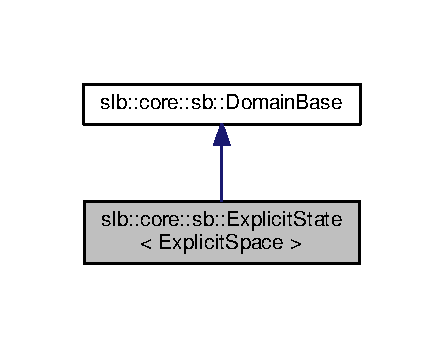
\includegraphics[width=213pt]{structslb_1_1core_1_1sb_1_1ExplicitState__inherit__graph}
\end{center}
\end{figure}


Collaboration diagram for slb\+:\+:core\+:\+:sb\+:\+:Explicit\+State$<$ Explicit\+Space $>$\+:\nopagebreak
\begin{figure}[H]
\begin{center}
\leavevmode
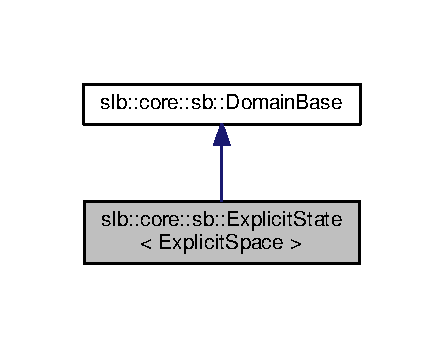
\includegraphics[width=213pt]{structslb_1_1core_1_1sb_1_1ExplicitState__coll__graph}
\end{center}
\end{figure}
\subsubsection*{Public Types}
\begin{DoxyCompactItemize}
\item 
using \hyperlink{structslb_1_1core_1_1sb_1_1ExplicitState_ae36e0763ad9b7ee7407aa316d4c64f14}{Cost\+Type} = typename Explicit\+Space\+::\+Cost\+Type\hypertarget{structslb_1_1core_1_1sb_1_1ExplicitState_ae36e0763ad9b7ee7407aa316d4c64f14}{}\label{structslb_1_1core_1_1sb_1_1ExplicitState_ae36e0763ad9b7ee7407aa316d4c64f14}

\begin{DoxyCompactList}\small\item\em The type representing the cost of actions in the domain. \end{DoxyCompactList}\item 
using \hyperlink{structslb_1_1core_1_1sb_1_1ExplicitState_ac92f2c174f45d0fd4276916906b4e8b7}{My\+Type} = \hyperlink{structslb_1_1core_1_1sb_1_1ExplicitState}{Explicit\+State}\hypertarget{structslb_1_1core_1_1sb_1_1ExplicitState_ac92f2c174f45d0fd4276916906b4e8b7}{}\label{structslb_1_1core_1_1sb_1_1ExplicitState_ac92f2c174f45d0fd4276916906b4e8b7}

\begin{DoxyCompactList}\small\item\em The type of a state in an explicit domain. \end{DoxyCompactList}\item 
using \hyperlink{structslb_1_1core_1_1sb_1_1ExplicitState_a0db984d44f46c477a6df3c9b062925f9}{Location} = typename Explicit\+Space\+::\+Location\hypertarget{structslb_1_1core_1_1sb_1_1ExplicitState_a0db984d44f46c477a6df3c9b062925f9}{}\label{structslb_1_1core_1_1sb_1_1ExplicitState_a0db984d44f46c477a6df3c9b062925f9}

\begin{DoxyCompactList}\small\item\em The type used internally by {\ttfamily Explicit\+Space} to represent a state. To distinguish such a state from the state type used by search algorithms, we call the former {\ttfamily location}. \end{DoxyCompactList}\end{DoxyCompactItemize}
\subsubsection*{Public Member Functions}
\begin{DoxyCompactItemize}
\item 
\hyperlink{structslb_1_1core_1_1sb_1_1ExplicitState_a8d4e4a73d0760f49b275e2661f759fcf}{Explicit\+State} ()\hypertarget{structslb_1_1core_1_1sb_1_1ExplicitState_a8d4e4a73d0760f49b275e2661f759fcf}{}\label{structslb_1_1core_1_1sb_1_1ExplicitState_a8d4e4a73d0760f49b275e2661f759fcf}

\begin{DoxyCompactList}\small\item\em Initialize the location with the space\textquotesingle{}s default. \end{DoxyCompactList}\item 
\hyperlink{structslb_1_1core_1_1sb_1_1ExplicitState_abb5dc932345986e03ba3afae41408086}{Explicit\+State} (const \hyperlink{structslb_1_1core_1_1sb_1_1ExplicitState_a0db984d44f46c477a6df3c9b062925f9}{Location} \&loc)
\begin{DoxyCompactList}\small\item\em Initialize to the given location. \end{DoxyCompactList}\item 
\hyperlink{structslb_1_1core_1_1sb_1_1ExplicitState_a9ba10a1c18e845a63ac6aa5b5669adde}{Explicit\+State} (const std\+::string \&s)
\begin{DoxyCompactList}\small\item\em Initialize based on the string describing the state. \end{DoxyCompactList}\item 
\hyperlink{structslb_1_1core_1_1sb_1_1ExplicitState_a269a858c6fcf90f39f363326c5a977de}{Explicit\+State} (const \hyperlink{structslb_1_1core_1_1sb_1_1ExplicitState_ac92f2c174f45d0fd4276916906b4e8b7}{My\+Type} \&)=default\hypertarget{structslb_1_1core_1_1sb_1_1ExplicitState_a269a858c6fcf90f39f363326c5a977de}{}\label{structslb_1_1core_1_1sb_1_1ExplicitState_a269a858c6fcf90f39f363326c5a977de}

\begin{DoxyCompactList}\small\item\em Default copy constructor. \end{DoxyCompactList}\item 
\hyperlink{structslb_1_1core_1_1sb_1_1ExplicitState}{Explicit\+State} \& \hyperlink{structslb_1_1core_1_1sb_1_1ExplicitState_a6193bf706a682ba07f80aef31c419875}{operator=} (const \hyperlink{structslb_1_1core_1_1sb_1_1ExplicitState_ac92f2c174f45d0fd4276916906b4e8b7}{My\+Type} \&)=default\hypertarget{structslb_1_1core_1_1sb_1_1ExplicitState_a6193bf706a682ba07f80aef31c419875}{}\label{structslb_1_1core_1_1sb_1_1ExplicitState_a6193bf706a682ba07f80aef31c419875}

\begin{DoxyCompactList}\small\item\em Default assignment operator. \end{DoxyCompactList}\item 
{\footnotesize template$<$class Neighbor $>$ }\\std\+::vector$<$ Neighbor $>$ \hyperlink{structslb_1_1core_1_1sb_1_1ExplicitState_ae4fddaedd8936221f4c92dd5607e5d2b}{location\+Successors} () const 
\begin{DoxyCompactList}\small\item\em Computes the neighbors of the state. \end{DoxyCompactList}\item 
std\+::size\+\_\+t \hyperlink{structslb_1_1core_1_1sb_1_1ExplicitState_a982d9c77e71b3d0e64c0b41d422fa32f}{hash} () const 
\begin{DoxyCompactList}\small\item\em Computes the hash code of the state. \end{DoxyCompactList}\item 
const \hyperlink{structslb_1_1core_1_1sb_1_1ExplicitState_a0db984d44f46c477a6df3c9b062925f9}{Location} \& \hyperlink{structslb_1_1core_1_1sb_1_1ExplicitState_ac75620076983d8d35de370bdb0ce1f96}{raw} () const 
\begin{DoxyCompactList}\small\item\em Returns the location. \end{DoxyCompactList}\item 
{\footnotesize template$<$typename Stream $>$ }\\Stream \& \hyperlink{structslb_1_1core_1_1sb_1_1ExplicitState_ac9f4d6972a1437dd41b74a4608438310}{dump} (Stream \&o) const 
\begin{DoxyCompactList}\small\item\em Dumps the node the state to the given stream. \end{DoxyCompactList}\item 
bool \hyperlink{structslb_1_1core_1_1sb_1_1ExplicitState_ac7e19ab8c118d1c28e45a2848bdb1cf5}{operator==} (const \hyperlink{structslb_1_1core_1_1sb_1_1ExplicitState_ac92f2c174f45d0fd4276916906b4e8b7}{My\+Type} \&rhs) const 
\begin{DoxyCompactList}\small\item\em The equality operator. \end{DoxyCompactList}\end{DoxyCompactItemize}
\subsubsection*{Static Public Member Functions}
\begin{DoxyCompactItemize}
\item 
static void \hyperlink{structslb_1_1core_1_1sb_1_1ExplicitState_af02f7ca680be7105f85fd17d7fea87e7}{init\+Space} (const std\+::string \&file\+Name)
\begin{DoxyCompactList}\small\item\em Sets the space (i.\+e. an instance of Explicit\+Space) for this state class by reading it from the given file. \end{DoxyCompactList}\item 
static \hyperlink{structslb_1_1core_1_1sb_1_1ExplicitState_a0db984d44f46c477a6df3c9b062925f9}{Location} \hyperlink{structslb_1_1core_1_1sb_1_1ExplicitState_a48457e70133ab1b4d6357b221917cc11}{random} ()
\begin{DoxyCompactList}\small\item\em Returns a random location. \end{DoxyCompactList}\item 
static const std\+::unique\+\_\+ptr$<$ Explicit\+Space $>$ \& \hyperlink{structslb_1_1core_1_1sb_1_1ExplicitState_a18c5da0e54b1562f2a224f414694a80f}{space} ()
\begin{DoxyCompactList}\small\item\em Returns the space (i.\+e. an instance of Explicit\+Space) of this state class. \end{DoxyCompactList}\end{DoxyCompactItemize}
\subsubsection*{Private Attributes}
\begin{DoxyCompactItemize}
\item 
\hyperlink{structslb_1_1core_1_1sb_1_1ExplicitState_a0db984d44f46c477a6df3c9b062925f9}{Location} \hyperlink{structslb_1_1core_1_1sb_1_1ExplicitState_ae5a70068fa1e66171e4bd1a4c33bd02d}{loc\+\_\+}\hypertarget{structslb_1_1core_1_1sb_1_1ExplicitState_ae5a70068fa1e66171e4bd1a4c33bd02d}{}\label{structslb_1_1core_1_1sb_1_1ExplicitState_ae5a70068fa1e66171e4bd1a4c33bd02d}

\begin{DoxyCompactList}\small\item\em The location, which is the raw state as used by {\ttfamily Explicit\+Space}. \end{DoxyCompactList}\end{DoxyCompactItemize}
\subsubsection*{Static Private Attributes}
\begin{DoxyCompactItemize}
\item 
static std\+::unique\+\_\+ptr$<$ Explicit\+Space $>$ \hyperlink{structslb_1_1core_1_1sb_1_1ExplicitState_aec671efc84838fa7d339cb7316758e59}{space\+\_\+} = nullptr\hypertarget{structslb_1_1core_1_1sb_1_1ExplicitState_aec671efc84838fa7d339cb7316758e59}{}\label{structslb_1_1core_1_1sb_1_1ExplicitState_aec671efc84838fa7d339cb7316758e59}

\begin{DoxyCompactList}\small\item\em The explicit space. \end{DoxyCompactList}\end{DoxyCompactItemize}


\subsubsection{Detailed Description}
\subsubsection*{template$<$class Explicit\+Space$>$\\*
struct slb\+::core\+::sb\+::\+Explicit\+State$<$ Explicit\+Space $>$}

The base class for a state in an explicit domain. It can be viewed as a wrapper for the location type defined by the explicit domain. 


\begin{DoxyTemplParams}{Template Parameters}
{\em Explicit\+Space} & The type for storing the explicit space (e.\+g. a map). \\
\hline
\end{DoxyTemplParams}


Definition at line 16 of file explicit\+\_\+state.\+h.



\subsubsection{Constructor \& Destructor Documentation}
\index{slb\+::core\+::sb\+::\+Explicit\+State@{slb\+::core\+::sb\+::\+Explicit\+State}!Explicit\+State@{Explicit\+State}}
\index{Explicit\+State@{Explicit\+State}!slb\+::core\+::sb\+::\+Explicit\+State@{slb\+::core\+::sb\+::\+Explicit\+State}}
\paragraph[{\texorpdfstring{Explicit\+State(const Location \&loc)}{ExplicitState(const Location &loc)}}]{\setlength{\rightskip}{0pt plus 5cm}template$<$class Explicit\+Space$>$ {\bf slb\+::core\+::sb\+::\+Explicit\+State}$<$ Explicit\+Space $>$\+::{\bf Explicit\+State} (
\begin{DoxyParamCaption}
\item[{const {\bf Location} \&}]{loc}
\end{DoxyParamCaption}
)\hspace{0.3cm}{\ttfamily [inline]}, {\ttfamily [explicit]}}\hypertarget{structslb_1_1core_1_1sb_1_1ExplicitState_abb5dc932345986e03ba3afae41408086}{}\label{structslb_1_1core_1_1sb_1_1ExplicitState_abb5dc932345986e03ba3afae41408086}


Initialize to the given location. 


\begin{DoxyParams}{Parameters}
{\em loc} & The given location. \\
\hline
\end{DoxyParams}


Definition at line 33 of file explicit\+\_\+state.\+h.

\index{slb\+::core\+::sb\+::\+Explicit\+State@{slb\+::core\+::sb\+::\+Explicit\+State}!Explicit\+State@{Explicit\+State}}
\index{Explicit\+State@{Explicit\+State}!slb\+::core\+::sb\+::\+Explicit\+State@{slb\+::core\+::sb\+::\+Explicit\+State}}
\paragraph[{\texorpdfstring{Explicit\+State(const std\+::string \&s)}{ExplicitState(const std::string &s)}}]{\setlength{\rightskip}{0pt plus 5cm}template$<$class Explicit\+Space$>$ {\bf slb\+::core\+::sb\+::\+Explicit\+State}$<$ Explicit\+Space $>$\+::{\bf Explicit\+State} (
\begin{DoxyParamCaption}
\item[{const std\+::string \&}]{s}
\end{DoxyParamCaption}
)\hspace{0.3cm}{\ttfamily [inline]}, {\ttfamily [explicit]}}\hypertarget{structslb_1_1core_1_1sb_1_1ExplicitState_a9ba10a1c18e845a63ac6aa5b5669adde}{}\label{structslb_1_1core_1_1sb_1_1ExplicitState_a9ba10a1c18e845a63ac6aa5b5669adde}


Initialize based on the string describing the state. 


\begin{DoxyParams}{Parameters}
{\em s} & The string describing the state. \\
\hline
\end{DoxyParams}


Definition at line 37 of file explicit\+\_\+state.\+h.



\subsubsection{Member Function Documentation}
\index{slb\+::core\+::sb\+::\+Explicit\+State@{slb\+::core\+::sb\+::\+Explicit\+State}!dump@{dump}}
\index{dump@{dump}!slb\+::core\+::sb\+::\+Explicit\+State@{slb\+::core\+::sb\+::\+Explicit\+State}}
\paragraph[{\texorpdfstring{dump(\+Stream \&o) const }{dump(Stream &o) const }}]{\setlength{\rightskip}{0pt plus 5cm}template$<$class Explicit\+Space$>$ template$<$typename Stream $>$ Stream\& {\bf slb\+::core\+::sb\+::\+Explicit\+State}$<$ Explicit\+Space $>$\+::dump (
\begin{DoxyParamCaption}
\item[{Stream \&}]{o}
\end{DoxyParamCaption}
) const\hspace{0.3cm}{\ttfamily [inline]}}\hypertarget{structslb_1_1core_1_1sb_1_1ExplicitState_ac9f4d6972a1437dd41b74a4608438310}{}\label{structslb_1_1core_1_1sb_1_1ExplicitState_ac9f4d6972a1437dd41b74a4608438310}


Dumps the node the state to the given stream. 


\begin{DoxyTemplParams}{Template Parameters}
{\em Stream} & The output stream type. \\
\hline
\end{DoxyTemplParams}

\begin{DoxyParams}{Parameters}
{\em o} & The output stream. \\
\hline
\end{DoxyParams}


Definition at line 71 of file explicit\+\_\+state.\+h.

\index{slb\+::core\+::sb\+::\+Explicit\+State@{slb\+::core\+::sb\+::\+Explicit\+State}!hash@{hash}}
\index{hash@{hash}!slb\+::core\+::sb\+::\+Explicit\+State@{slb\+::core\+::sb\+::\+Explicit\+State}}
\paragraph[{\texorpdfstring{hash() const }{hash() const }}]{\setlength{\rightskip}{0pt plus 5cm}template$<$class Explicit\+Space$>$ std\+::size\+\_\+t {\bf slb\+::core\+::sb\+::\+Explicit\+State}$<$ Explicit\+Space $>$\+::hash (
\begin{DoxyParamCaption}
{}
\end{DoxyParamCaption}
) const\hspace{0.3cm}{\ttfamily [inline]}}\hypertarget{structslb_1_1core_1_1sb_1_1ExplicitState_a982d9c77e71b3d0e64c0b41d422fa32f}{}\label{structslb_1_1core_1_1sb_1_1ExplicitState_a982d9c77e71b3d0e64c0b41d422fa32f}


Computes the hash code of the state. 

\begin{DoxyReturn}{Returns}
The hash code of the state. 
\end{DoxyReturn}


Definition at line 58 of file explicit\+\_\+state.\+h.

\index{slb\+::core\+::sb\+::\+Explicit\+State@{slb\+::core\+::sb\+::\+Explicit\+State}!init\+Space@{init\+Space}}
\index{init\+Space@{init\+Space}!slb\+::core\+::sb\+::\+Explicit\+State@{slb\+::core\+::sb\+::\+Explicit\+State}}
\paragraph[{\texorpdfstring{init\+Space(const std\+::string \&file\+Name)}{initSpace(const std::string &fileName)}}]{\setlength{\rightskip}{0pt plus 5cm}template$<$class Explicit\+Space$>$ static void {\bf slb\+::core\+::sb\+::\+Explicit\+State}$<$ Explicit\+Space $>$\+::init\+Space (
\begin{DoxyParamCaption}
\item[{const std\+::string \&}]{file\+Name}
\end{DoxyParamCaption}
)\hspace{0.3cm}{\ttfamily [inline]}, {\ttfamily [static]}}\hypertarget{structslb_1_1core_1_1sb_1_1ExplicitState_af02f7ca680be7105f85fd17d7fea87e7}{}\label{structslb_1_1core_1_1sb_1_1ExplicitState_af02f7ca680be7105f85fd17d7fea87e7}


Sets the space (i.\+e. an instance of Explicit\+Space) for this state class by reading it from the given file. 


\begin{DoxyParams}{Parameters}
{\em file\+Name} & The name of the file to read the space from. \\
\hline
\end{DoxyParams}


Definition at line 84 of file explicit\+\_\+state.\+h.

\index{slb\+::core\+::sb\+::\+Explicit\+State@{slb\+::core\+::sb\+::\+Explicit\+State}!location\+Successors@{location\+Successors}}
\index{location\+Successors@{location\+Successors}!slb\+::core\+::sb\+::\+Explicit\+State@{slb\+::core\+::sb\+::\+Explicit\+State}}
\paragraph[{\texorpdfstring{location\+Successors() const }{locationSuccessors() const }}]{\setlength{\rightskip}{0pt plus 5cm}template$<$class Explicit\+Space$>$ template$<$class Neighbor $>$ std\+::vector$<$Neighbor$>$ {\bf slb\+::core\+::sb\+::\+Explicit\+State}$<$ Explicit\+Space $>$\+::location\+Successors (
\begin{DoxyParamCaption}
{}
\end{DoxyParamCaption}
) const\hspace{0.3cm}{\ttfamily [inline]}}\hypertarget{structslb_1_1core_1_1sb_1_1ExplicitState_ae4fddaedd8936221f4c92dd5607e5d2b}{}\label{structslb_1_1core_1_1sb_1_1ExplicitState_ae4fddaedd8936221f4c92dd5607e5d2b}


Computes the neighbors of the state. 


\begin{DoxyTemplParams}{Template Parameters}
{\em Neighbor} & The type for representing a single neighbor state. \\
\hline
\end{DoxyTemplParams}
\begin{DoxyReturn}{Returns}
Vector of neighbors of the state. 
\end{DoxyReturn}


Definition at line 49 of file explicit\+\_\+state.\+h.

\index{slb\+::core\+::sb\+::\+Explicit\+State@{slb\+::core\+::sb\+::\+Explicit\+State}!operator==@{operator==}}
\index{operator==@{operator==}!slb\+::core\+::sb\+::\+Explicit\+State@{slb\+::core\+::sb\+::\+Explicit\+State}}
\paragraph[{\texorpdfstring{operator==(const My\+Type \&rhs) const }{operator==(const MyType &rhs) const }}]{\setlength{\rightskip}{0pt plus 5cm}template$<$class Explicit\+Space$>$ bool {\bf slb\+::core\+::sb\+::\+Explicit\+State}$<$ Explicit\+Space $>$\+::operator== (
\begin{DoxyParamCaption}
\item[{const {\bf My\+Type} \&}]{rhs}
\end{DoxyParamCaption}
) const\hspace{0.3cm}{\ttfamily [inline]}}\hypertarget{structslb_1_1core_1_1sb_1_1ExplicitState_ac7e19ab8c118d1c28e45a2848bdb1cf5}{}\label{structslb_1_1core_1_1sb_1_1ExplicitState_ac7e19ab8c118d1c28e45a2848bdb1cf5}


The equality operator. 


\begin{DoxyParams}{Parameters}
{\em rhs} & The right-\/hand side of the operator. \\
\hline
\end{DoxyParams}


Definition at line 77 of file explicit\+\_\+state.\+h.

\index{slb\+::core\+::sb\+::\+Explicit\+State@{slb\+::core\+::sb\+::\+Explicit\+State}!random@{random}}
\index{random@{random}!slb\+::core\+::sb\+::\+Explicit\+State@{slb\+::core\+::sb\+::\+Explicit\+State}}
\paragraph[{\texorpdfstring{random()}{random()}}]{\setlength{\rightskip}{0pt plus 5cm}template$<$class Explicit\+Space$>$ static {\bf Location} {\bf slb\+::core\+::sb\+::\+Explicit\+State}$<$ Explicit\+Space $>$\+::random (
\begin{DoxyParamCaption}
{}
\end{DoxyParamCaption}
)\hspace{0.3cm}{\ttfamily [inline]}, {\ttfamily [static]}}\hypertarget{structslb_1_1core_1_1sb_1_1ExplicitState_a48457e70133ab1b4d6357b221917cc11}{}\label{structslb_1_1core_1_1sb_1_1ExplicitState_a48457e70133ab1b4d6357b221917cc11}


Returns a random location. 

\begin{DoxyReturn}{Returns}
A random location. 
\end{DoxyReturn}


Definition at line 90 of file explicit\+\_\+state.\+h.

\index{slb\+::core\+::sb\+::\+Explicit\+State@{slb\+::core\+::sb\+::\+Explicit\+State}!raw@{raw}}
\index{raw@{raw}!slb\+::core\+::sb\+::\+Explicit\+State@{slb\+::core\+::sb\+::\+Explicit\+State}}
\paragraph[{\texorpdfstring{raw() const }{raw() const }}]{\setlength{\rightskip}{0pt plus 5cm}template$<$class Explicit\+Space$>$ const {\bf Location}\& {\bf slb\+::core\+::sb\+::\+Explicit\+State}$<$ Explicit\+Space $>$\+::raw (
\begin{DoxyParamCaption}
{}
\end{DoxyParamCaption}
) const\hspace{0.3cm}{\ttfamily [inline]}}\hypertarget{structslb_1_1core_1_1sb_1_1ExplicitState_ac75620076983d8d35de370bdb0ce1f96}{}\label{structslb_1_1core_1_1sb_1_1ExplicitState_ac75620076983d8d35de370bdb0ce1f96}


Returns the location. 

\begin{DoxyReturn}{Returns}
The location. 
\end{DoxyReturn}


Definition at line 65 of file explicit\+\_\+state.\+h.

\index{slb\+::core\+::sb\+::\+Explicit\+State@{slb\+::core\+::sb\+::\+Explicit\+State}!space@{space}}
\index{space@{space}!slb\+::core\+::sb\+::\+Explicit\+State@{slb\+::core\+::sb\+::\+Explicit\+State}}
\paragraph[{\texorpdfstring{space()}{space()}}]{\setlength{\rightskip}{0pt plus 5cm}template$<$class Explicit\+Space$>$ static const std\+::unique\+\_\+ptr$<$Explicit\+Space$>$\& {\bf slb\+::core\+::sb\+::\+Explicit\+State}$<$ Explicit\+Space $>$\+::space (
\begin{DoxyParamCaption}
{}
\end{DoxyParamCaption}
)\hspace{0.3cm}{\ttfamily [inline]}, {\ttfamily [static]}}\hypertarget{structslb_1_1core_1_1sb_1_1ExplicitState_a18c5da0e54b1562f2a224f414694a80f}{}\label{structslb_1_1core_1_1sb_1_1ExplicitState_a18c5da0e54b1562f2a224f414694a80f}


Returns the space (i.\+e. an instance of Explicit\+Space) of this state class. 

\begin{DoxyReturn}{Returns}
Const reference to unique pointer to the the space (i.\+e. an instance of Explicit\+Space) of this state class. 
\end{DoxyReturn}


Definition at line 96 of file explicit\+\_\+state.\+h.



The documentation for this struct was generated from the following file\+:\begin{DoxyCompactItemize}
\item 
core/search\+\_\+base/\hyperlink{explicit__state_8h}{explicit\+\_\+state.\+h}\end{DoxyCompactItemize}

\hypertarget{structslb_1_1core_1_1ui_1_1Filter}{}\subsection{slb\+:\+:core\+:\+:ui\+:\+:Filter$<$ Node $>$ Struct Template Reference}
\label{structslb_1_1core_1_1ui_1_1Filter}\index{slb\+::core\+::ui\+::\+Filter$<$ Node $>$@{slb\+::core\+::ui\+::\+Filter$<$ Node $>$}}


Composite filter. Does not filter out only the events not filtered out by any of the constituent filters.  




{\ttfamily \#include $<$filters.\+h$>$}



Inheritance diagram for slb\+:\+:core\+:\+:ui\+:\+:Filter$<$ Node $>$\+:\nopagebreak
\begin{figure}[H]
\begin{center}
\leavevmode
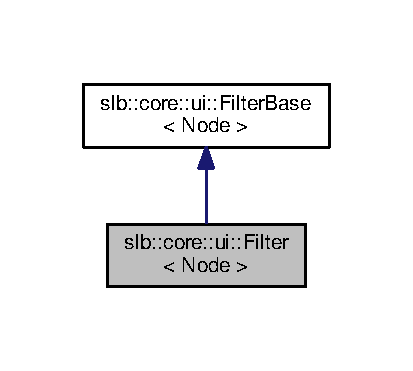
\includegraphics[width=198pt]{structslb_1_1core_1_1ui_1_1Filter__inherit__graph}
\end{center}
\end{figure}


Collaboration diagram for slb\+:\+:core\+:\+:ui\+:\+:Filter$<$ Node $>$\+:\nopagebreak
\begin{figure}[H]
\begin{center}
\leavevmode
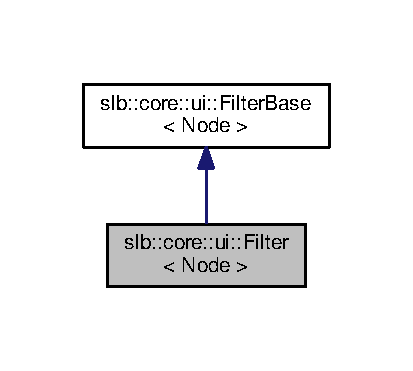
\includegraphics[width=198pt]{structslb_1_1core_1_1ui_1_1Filter__coll__graph}
\end{center}
\end{figure}
\subsubsection*{Public Types}
\begin{DoxyCompactItemize}
\item 
using \hyperlink{structslb_1_1core_1_1ui_1_1Filter_a6ffc4bc8847deda6db4be682318a01dc}{Event} = typename \hyperlink{structslb_1_1core_1_1ui_1_1FilterBase}{Filter\+Base}$<$ Node $>$\+::\hyperlink{structslb_1_1core_1_1ui_1_1FilterBase_a4cf70d819855984dc0e15a036e8b8a14}{Event}\hypertarget{structslb_1_1core_1_1ui_1_1Filter_a6ffc4bc8847deda6db4be682318a01dc}{}\label{structslb_1_1core_1_1ui_1_1Filter_a6ffc4bc8847deda6db4be682318a01dc}

\begin{DoxyCompactList}\small\item\em The type representing an event generated by the search algorithm. \end{DoxyCompactList}\item 
using \hyperlink{structslb_1_1core_1_1ui_1_1Filter_ab20ca413c82a4efc8dfe6000a56bf5f7}{State\+Shared\+Ptr} = typename \hyperlink{structslb_1_1core_1_1ui_1_1FilterBase}{Filter\+Base}$<$ Node $>$\+::\hyperlink{structslb_1_1core_1_1ui_1_1FilterBase_abb00418d744ad7aaa7c9333ec1dc2064}{State\+Shared\+Ptr}\hypertarget{structslb_1_1core_1_1ui_1_1Filter_ab20ca413c82a4efc8dfe6000a56bf5f7}{}\label{structslb_1_1core_1_1ui_1_1Filter_ab20ca413c82a4efc8dfe6000a56bf5f7}

\begin{DoxyCompactList}\small\item\em Smart pointer to state type representing the domain. \end{DoxyCompactList}\end{DoxyCompactItemize}
\subsubsection*{Public Member Functions}
\begin{DoxyCompactItemize}
\item 
\hyperlink{structslb_1_1core_1_1ui_1_1Filter_a83a648e702ab05ad75651b7e47b1e4a0}{Filter} (const std\+::vector$<$ std\+::string $>$ \&strings)\hypertarget{structslb_1_1core_1_1ui_1_1Filter_a83a648e702ab05ad75651b7e47b1e4a0}{}\label{structslb_1_1core_1_1ui_1_1Filter_a83a648e702ab05ad75651b7e47b1e4a0}

\begin{DoxyCompactList}\small\item\em Initializes the filter to only filter based on description strings of events. \end{DoxyCompactList}\item 
\hyperlink{structslb_1_1core_1_1ui_1_1FilterEventStr}{Filter\+Event\+Str}$<$ Node $>$ \& \hyperlink{structslb_1_1core_1_1ui_1_1Filter_a6682eb7f1f16cbac241433ba765ca3e7}{filter\+Event\+Str} ()
\begin{DoxyCompactList}\small\item\em Returns the constituent filter that filters based on description strings of events. \end{DoxyCompactList}\item 
\hyperlink{structslb_1_1core_1_1ui_1_1FilterState}{Filter\+State}$<$ Node $>$ \& \hyperlink{structslb_1_1core_1_1ui_1_1Filter_a3eefa14ffdef3dd5bc1541356b3b37eb}{filter\+State} ()
\begin{DoxyCompactList}\small\item\em Returns the constituent filter that filters based on the list of the states of interest. \end{DoxyCompactList}\item 
virtual bool \hyperlink{structslb_1_1core_1_1ui_1_1Filter_a847ebebdfe826a3d0c26a52b13e1ba26}{in} (const \hyperlink{structslb_1_1core_1_1ui_1_1FilterBase_a4cf70d819855984dc0e15a036e8b8a14}{Event} \&e) const override
\begin{DoxyCompactList}\small\item\em Determines whether the given event is not filtered out. \end{DoxyCompactList}\end{DoxyCompactItemize}
\subsubsection*{Private Attributes}
\begin{DoxyCompactItemize}
\item 
\hyperlink{structslb_1_1core_1_1ui_1_1FilterEventStr}{Filter\+Event\+Str}$<$ Node $>$ \hyperlink{structslb_1_1core_1_1ui_1_1Filter_a52b9c45741ded8c395ade5838afab4fa}{filter\+Event\+Str\+\_\+}\hypertarget{structslb_1_1core_1_1ui_1_1Filter_a52b9c45741ded8c395ade5838afab4fa}{}\label{structslb_1_1core_1_1ui_1_1Filter_a52b9c45741ded8c395ade5838afab4fa}

\begin{DoxyCompactList}\small\item\em The constituent filter that filters based on description strings of events. \end{DoxyCompactList}\item 
\hyperlink{structslb_1_1core_1_1ui_1_1FilterState}{Filter\+State}$<$ Node $>$ \hyperlink{structslb_1_1core_1_1ui_1_1Filter_a2b8220ef5cd590fa9e3e11b8ce751988}{filter\+State\+\_\+}\hypertarget{structslb_1_1core_1_1ui_1_1Filter_a2b8220ef5cd590fa9e3e11b8ce751988}{}\label{structslb_1_1core_1_1ui_1_1Filter_a2b8220ef5cd590fa9e3e11b8ce751988}

\begin{DoxyCompactList}\small\item\em The constituent filter that filters based on the list of the states of interest. \end{DoxyCompactList}\item 
std\+::vector$<$ \hyperlink{structslb_1_1core_1_1ui_1_1FilterBase}{Filter\+Base}$<$ Node $>$ $\ast$ $>$ \hyperlink{structslb_1_1core_1_1ui_1_1Filter_a95b665853749f2384f67507bd024f771}{filters\+\_\+}\hypertarget{structslb_1_1core_1_1ui_1_1Filter_a95b665853749f2384f67507bd024f771}{}\label{structslb_1_1core_1_1ui_1_1Filter_a95b665853749f2384f67507bd024f771}

\begin{DoxyCompactList}\small\item\em The constituent filters. \end{DoxyCompactList}\end{DoxyCompactItemize}


\subsubsection{Detailed Description}
\subsubsection*{template$<$class Node$>$\\*
struct slb\+::core\+::ui\+::\+Filter$<$ Node $>$}

Composite filter. Does not filter out only the events not filtered out by any of the constituent filters. 


\begin{DoxyTemplParams}{Template Parameters}
{\em Node} & The search node type. \\
\hline
\end{DoxyTemplParams}


Definition at line 113 of file filters.\+h.



\subsubsection{Member Function Documentation}
\index{slb\+::core\+::ui\+::\+Filter@{slb\+::core\+::ui\+::\+Filter}!filter\+Event\+Str@{filter\+Event\+Str}}
\index{filter\+Event\+Str@{filter\+Event\+Str}!slb\+::core\+::ui\+::\+Filter@{slb\+::core\+::ui\+::\+Filter}}
\paragraph[{\texorpdfstring{filter\+Event\+Str()}{filterEventStr()}}]{\setlength{\rightskip}{0pt plus 5cm}template$<$class Node$>$ {\bf Filter\+Event\+Str}$<$Node$>$\& {\bf slb\+::core\+::ui\+::\+Filter}$<$ Node $>$\+::filter\+Event\+Str (
\begin{DoxyParamCaption}
{}
\end{DoxyParamCaption}
)\hspace{0.3cm}{\ttfamily [inline]}}\hypertarget{structslb_1_1core_1_1ui_1_1Filter_a6682eb7f1f16cbac241433ba765ca3e7}{}\label{structslb_1_1core_1_1ui_1_1Filter_a6682eb7f1f16cbac241433ba765ca3e7}


Returns the constituent filter that filters based on description strings of events. 

\begin{DoxyReturn}{Returns}
Reference to the constituent filter that filters based on description strings of events. 
\end{DoxyReturn}


Definition at line 130 of file filters.\+h.

\index{slb\+::core\+::ui\+::\+Filter@{slb\+::core\+::ui\+::\+Filter}!filter\+State@{filter\+State}}
\index{filter\+State@{filter\+State}!slb\+::core\+::ui\+::\+Filter@{slb\+::core\+::ui\+::\+Filter}}
\paragraph[{\texorpdfstring{filter\+State()}{filterState()}}]{\setlength{\rightskip}{0pt plus 5cm}template$<$class Node$>$ {\bf Filter\+State}$<$Node$>$\& {\bf slb\+::core\+::ui\+::\+Filter}$<$ Node $>$\+::filter\+State (
\begin{DoxyParamCaption}
{}
\end{DoxyParamCaption}
)\hspace{0.3cm}{\ttfamily [inline]}}\hypertarget{structslb_1_1core_1_1ui_1_1Filter_a3eefa14ffdef3dd5bc1541356b3b37eb}{}\label{structslb_1_1core_1_1ui_1_1Filter_a3eefa14ffdef3dd5bc1541356b3b37eb}


Returns the constituent filter that filters based on the list of the states of interest. 

\begin{DoxyReturn}{Returns}
Reference to the constituent filter that filters based the list of the states of interest. 
\end{DoxyReturn}


Definition at line 138 of file filters.\+h.

\index{slb\+::core\+::ui\+::\+Filter@{slb\+::core\+::ui\+::\+Filter}!in@{in}}
\index{in@{in}!slb\+::core\+::ui\+::\+Filter@{slb\+::core\+::ui\+::\+Filter}}
\paragraph[{\texorpdfstring{in(const Event \&e) const override}{in(const Event &e) const override}}]{\setlength{\rightskip}{0pt plus 5cm}template$<$class Node$>$ virtual bool {\bf slb\+::core\+::ui\+::\+Filter}$<$ Node $>$\+::in (
\begin{DoxyParamCaption}
\item[{const {\bf Event} \&}]{e}
\end{DoxyParamCaption}
) const\hspace{0.3cm}{\ttfamily [inline]}, {\ttfamily [override]}, {\ttfamily [virtual]}}\hypertarget{structslb_1_1core_1_1ui_1_1Filter_a847ebebdfe826a3d0c26a52b13e1ba26}{}\label{structslb_1_1core_1_1ui_1_1Filter_a847ebebdfe826a3d0c26a52b13e1ba26}


Determines whether the given event is not filtered out. 


\begin{DoxyParams}{Parameters}
{\em e} & The event of interest. \\
\hline
\end{DoxyParams}
\begin{DoxyReturn}{Returns}
{\ttfamily true} if the given event is not filtered out. 
\end{DoxyReturn}


Implements \hyperlink{structslb_1_1core_1_1ui_1_1FilterBase_af89dfa7be8a61ad95f688b43f40379ad}{slb\+::core\+::ui\+::\+Filter\+Base$<$ Node $>$}.



Definition at line 145 of file filters.\+h.



The documentation for this struct was generated from the following file\+:\begin{DoxyCompactItemize}
\item 
core/user\+\_\+interface/\hyperlink{filters_8h}{filters.\+h}\end{DoxyCompactItemize}

\hypertarget{structslb_1_1core_1_1ui_1_1FilterBase}{}\subsection{slb\+:\+:core\+:\+:ui\+:\+:Filter\+Base$<$ Node $>$ Struct Template Reference}
\label{structslb_1_1core_1_1ui_1_1FilterBase}\index{slb\+::core\+::ui\+::\+Filter\+Base$<$ Node $>$@{slb\+::core\+::ui\+::\+Filter\+Base$<$ Node $>$}}


The abstract base for all filters.  




{\ttfamily \#include $<$filters.\+h$>$}



Inheritance diagram for slb\+:\+:core\+:\+:ui\+:\+:Filter\+Base$<$ Node $>$\+:\nopagebreak
\begin{figure}[H]
\begin{center}
\leavevmode
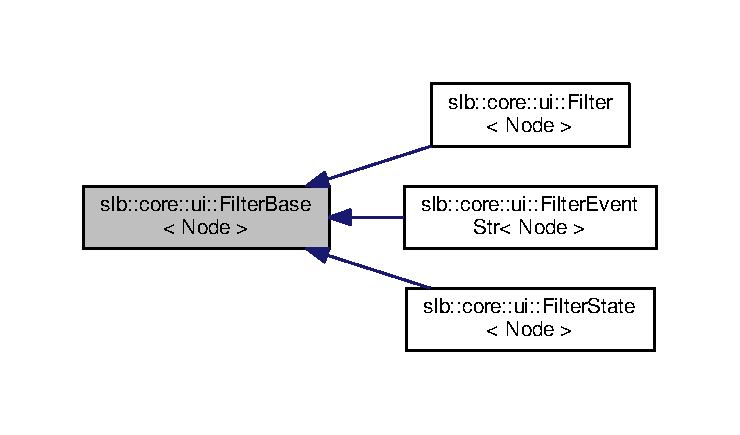
\includegraphics[width=350pt]{structslb_1_1core_1_1ui_1_1FilterBase__inherit__graph}
\end{center}
\end{figure}
\subsubsection*{Public Types}
\begin{DoxyCompactItemize}
\item 
using \hyperlink{structslb_1_1core_1_1ui_1_1FilterBase_a4cf70d819855984dc0e15a036e8b8a14}{Event} = typename \hyperlink{structslb_1_1core_1_1ui_1_1EventBase}{Event\+Base}$<$ Node $>$\+::\hyperlink{structslb_1_1core_1_1ui_1_1FilterBase_a4cf70d819855984dc0e15a036e8b8a14}{Event}\hypertarget{structslb_1_1core_1_1ui_1_1FilterBase_a4cf70d819855984dc0e15a036e8b8a14}{}\label{structslb_1_1core_1_1ui_1_1FilterBase_a4cf70d819855984dc0e15a036e8b8a14}

\begin{DoxyCompactList}\small\item\em The type representing an event generated by the search algorithm. \end{DoxyCompactList}\item 
using \hyperlink{structslb_1_1core_1_1ui_1_1FilterBase_abb00418d744ad7aaa7c9333ec1dc2064}{State\+Shared\+Ptr} = typename \hyperlink{structslb_1_1core_1_1ui_1_1EventBase}{Event\+Base}$<$ Node $>$\+::\hyperlink{structslb_1_1core_1_1ui_1_1FilterBase_abb00418d744ad7aaa7c9333ec1dc2064}{State\+Shared\+Ptr}\hypertarget{structslb_1_1core_1_1ui_1_1FilterBase_abb00418d744ad7aaa7c9333ec1dc2064}{}\label{structslb_1_1core_1_1ui_1_1FilterBase_abb00418d744ad7aaa7c9333ec1dc2064}

\begin{DoxyCompactList}\small\item\em Smart pointer to state type representing the domain. \end{DoxyCompactList}\end{DoxyCompactItemize}
\subsubsection*{Public Member Functions}
\begin{DoxyCompactItemize}
\item 
virtual bool \hyperlink{structslb_1_1core_1_1ui_1_1FilterBase_af89dfa7be8a61ad95f688b43f40379ad}{in} (const \hyperlink{structslb_1_1core_1_1ui_1_1FilterBase_a4cf70d819855984dc0e15a036e8b8a14}{Event} \&e) const =0
\begin{DoxyCompactList}\small\item\em Determines whether the given event is not filtered out. \end{DoxyCompactList}\end{DoxyCompactItemize}


\subsubsection{Detailed Description}
\subsubsection*{template$<$class Node$>$\\*
struct slb\+::core\+::ui\+::\+Filter\+Base$<$ Node $>$}

The abstract base for all filters. 


\begin{DoxyTemplParams}{Template Parameters}
{\em Node} & The search node type. It is needed since some filters might operate on the information stored with the node. \\
\hline
\end{DoxyTemplParams}


Definition at line 16 of file filters.\+h.



\subsubsection{Member Function Documentation}
\index{slb\+::core\+::ui\+::\+Filter\+Base@{slb\+::core\+::ui\+::\+Filter\+Base}!in@{in}}
\index{in@{in}!slb\+::core\+::ui\+::\+Filter\+Base@{slb\+::core\+::ui\+::\+Filter\+Base}}
\paragraph[{\texorpdfstring{in(const Event \&e) const =0}{in(const Event &e) const =0}}]{\setlength{\rightskip}{0pt plus 5cm}template$<$class Node$>$ virtual bool {\bf slb\+::core\+::ui\+::\+Filter\+Base}$<$ Node $>$\+::in (
\begin{DoxyParamCaption}
\item[{const {\bf Event} \&}]{e}
\end{DoxyParamCaption}
) const\hspace{0.3cm}{\ttfamily [pure virtual]}}\hypertarget{structslb_1_1core_1_1ui_1_1FilterBase_af89dfa7be8a61ad95f688b43f40379ad}{}\label{structslb_1_1core_1_1ui_1_1FilterBase_af89dfa7be8a61ad95f688b43f40379ad}


Determines whether the given event is not filtered out. 


\begin{DoxyParams}{Parameters}
{\em e} & The event of interest. \\
\hline
\end{DoxyParams}
\begin{DoxyReturn}{Returns}
{\ttfamily true} if the given event is not filtered out. 
\end{DoxyReturn}


Implemented in \hyperlink{structslb_1_1core_1_1ui_1_1Filter_a847ebebdfe826a3d0c26a52b13e1ba26}{slb\+::core\+::ui\+::\+Filter$<$ Node $>$}, \hyperlink{structslb_1_1core_1_1ui_1_1FilterState_abacffaaa5ed7700394e99ede2744323c}{slb\+::core\+::ui\+::\+Filter\+State$<$ Node $>$}, and \hyperlink{structslb_1_1core_1_1ui_1_1FilterEventStr_a293ba80691a7b507e8ad765e26da20a1}{slb\+::core\+::ui\+::\+Filter\+Event\+Str$<$ Node $>$}.



The documentation for this struct was generated from the following file\+:\begin{DoxyCompactItemize}
\item 
core/user\+\_\+interface/\hyperlink{filters_8h}{filters.\+h}\end{DoxyCompactItemize}

\hypertarget{structslb_1_1core_1_1ui_1_1FilterEventStr}{}\subsection{slb\+:\+:core\+:\+:ui\+:\+:Filter\+Event\+Str$<$ Node $>$ Struct Template Reference}
\label{structslb_1_1core_1_1ui_1_1FilterEventStr}\index{slb\+::core\+::ui\+::\+Filter\+Event\+Str$<$ Node $>$@{slb\+::core\+::ui\+::\+Filter\+Event\+Str$<$ Node $>$}}


Filters based on description strings of events.  




{\ttfamily \#include $<$filters.\+h$>$}



Inheritance diagram for slb\+:\+:core\+:\+:ui\+:\+:Filter\+Event\+Str$<$ Node $>$\+:\nopagebreak
\begin{figure}[H]
\begin{center}
\leavevmode
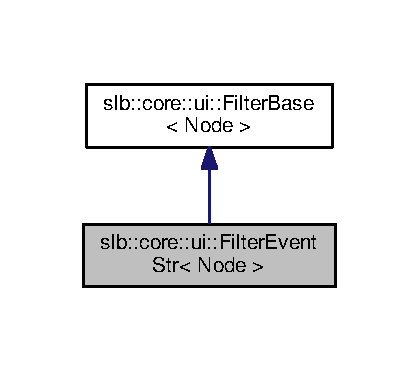
\includegraphics[width=201pt]{structslb_1_1core_1_1ui_1_1FilterEventStr__inherit__graph}
\end{center}
\end{figure}


Collaboration diagram for slb\+:\+:core\+:\+:ui\+:\+:Filter\+Event\+Str$<$ Node $>$\+:\nopagebreak
\begin{figure}[H]
\begin{center}
\leavevmode
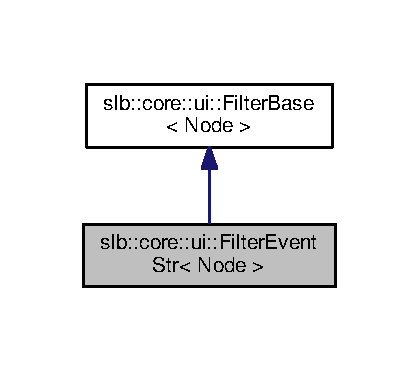
\includegraphics[width=201pt]{structslb_1_1core_1_1ui_1_1FilterEventStr__coll__graph}
\end{center}
\end{figure}
\subsubsection*{Public Types}
\begin{DoxyCompactItemize}
\item 
using \hyperlink{structslb_1_1core_1_1ui_1_1FilterEventStr_a98c36f7cb817340464bd1147005191b9}{Event} = typename \hyperlink{structslb_1_1core_1_1ui_1_1FilterBase}{Filter\+Base}$<$ Node $>$\+::\hyperlink{structslb_1_1core_1_1ui_1_1FilterBase_a4cf70d819855984dc0e15a036e8b8a14}{Event}\hypertarget{structslb_1_1core_1_1ui_1_1FilterEventStr_a98c36f7cb817340464bd1147005191b9}{}\label{structslb_1_1core_1_1ui_1_1FilterEventStr_a98c36f7cb817340464bd1147005191b9}

\begin{DoxyCompactList}\small\item\em The type representing an event generated by the search algorithm. \end{DoxyCompactList}\item 
using \hyperlink{structslb_1_1core_1_1ui_1_1FilterEventStr_a3948fefffa2744066ba7e927d36e6af5}{State\+Shared\+Ptr} = typename \hyperlink{structslb_1_1core_1_1ui_1_1FilterBase}{Filter\+Base}$<$ Node $>$\+::\hyperlink{structslb_1_1core_1_1ui_1_1FilterBase_abb00418d744ad7aaa7c9333ec1dc2064}{State\+Shared\+Ptr}\hypertarget{structslb_1_1core_1_1ui_1_1FilterEventStr_a3948fefffa2744066ba7e927d36e6af5}{}\label{structslb_1_1core_1_1ui_1_1FilterEventStr_a3948fefffa2744066ba7e927d36e6af5}

\begin{DoxyCompactList}\small\item\em Smart pointer to state type representing the domain. \end{DoxyCompactList}\end{DoxyCompactItemize}
\subsubsection*{Public Member Functions}
\begin{DoxyCompactItemize}
\item 
\hyperlink{structslb_1_1core_1_1ui_1_1FilterEventStr_ae3526ea4668a1ff0539eb94802b99a79}{Filter\+Event\+Str} (const std\+::vector$<$ std\+::string $>$ \&strings)
\begin{DoxyCompactList}\small\item\em Initializes the filter based on the description strings of events that should not be filtered out. \end{DoxyCompactList}\item 
virtual bool \hyperlink{structslb_1_1core_1_1ui_1_1FilterEventStr_a293ba80691a7b507e8ad765e26da20a1}{in} (const \hyperlink{structslb_1_1core_1_1ui_1_1FilterBase_a4cf70d819855984dc0e15a036e8b8a14}{Event} \&e) const 
\begin{DoxyCompactList}\small\item\em Determines whether the given event is not filtered out. \end{DoxyCompactList}\item 
void \hyperlink{structslb_1_1core_1_1ui_1_1FilterEventStr_accd872f69c9e216911b28b86e5750d79}{set} (const std\+::vector$<$ std\+::string $>$ \&strings)
\begin{DoxyCompactList}\small\item\em Sets the description strings of events that should not be filtered out. \end{DoxyCompactList}\item 
const std\+::vector$<$ std\+::string $>$ \& \hyperlink{structslb_1_1core_1_1ui_1_1FilterEventStr_a4e97c281a9ecbdbba3b427ed8eea76ee}{get} () const 
\begin{DoxyCompactList}\small\item\em Returns the description strings of events that should not be filtered out. \end{DoxyCompactList}\end{DoxyCompactItemize}
\subsubsection*{Private Attributes}
\begin{DoxyCompactItemize}
\item 
std\+::vector$<$ std\+::string $>$ \hyperlink{structslb_1_1core_1_1ui_1_1FilterEventStr_a0dc4d01a3e30f573f842a1766d559d33}{strings\+\_\+}\hypertarget{structslb_1_1core_1_1ui_1_1FilterEventStr_a0dc4d01a3e30f573f842a1766d559d33}{}\label{structslb_1_1core_1_1ui_1_1FilterEventStr_a0dc4d01a3e30f573f842a1766d559d33}

\begin{DoxyCompactList}\small\item\em The vector of description strings of events that should not be filtered out. \end{DoxyCompactList}\end{DoxyCompactItemize}


\subsubsection{Detailed Description}
\subsubsection*{template$<$class Node$>$\\*
struct slb\+::core\+::ui\+::\+Filter\+Event\+Str$<$ Node $>$}

Filters based on description strings of events. 


\begin{DoxyTemplParams}{Template Parameters}
{\em Node} & The search node type. \\
\hline
\end{DoxyTemplParams}


Definition at line 31 of file filters.\+h.



\subsubsection{Constructor \& Destructor Documentation}
\index{slb\+::core\+::ui\+::\+Filter\+Event\+Str@{slb\+::core\+::ui\+::\+Filter\+Event\+Str}!Filter\+Event\+Str@{Filter\+Event\+Str}}
\index{Filter\+Event\+Str@{Filter\+Event\+Str}!slb\+::core\+::ui\+::\+Filter\+Event\+Str@{slb\+::core\+::ui\+::\+Filter\+Event\+Str}}
\paragraph[{\texorpdfstring{Filter\+Event\+Str(const std\+::vector$<$ std\+::string $>$ \&strings)}{FilterEventStr(const std::vector< std::string > &strings)}}]{\setlength{\rightskip}{0pt plus 5cm}template$<$class Node$>$ {\bf slb\+::core\+::ui\+::\+Filter\+Event\+Str}$<$ Node $>$\+::{\bf Filter\+Event\+Str} (
\begin{DoxyParamCaption}
\item[{const std\+::vector$<$ std\+::string $>$ \&}]{strings}
\end{DoxyParamCaption}
)\hspace{0.3cm}{\ttfamily [inline]}}\hypertarget{structslb_1_1core_1_1ui_1_1FilterEventStr_ae3526ea4668a1ff0539eb94802b99a79}{}\label{structslb_1_1core_1_1ui_1_1FilterEventStr_ae3526ea4668a1ff0539eb94802b99a79}


Initializes the filter based on the description strings of events that should not be filtered out. 


\begin{DoxyParams}{Parameters}
{\em strings} & The description strings of events that should not be filtered out. \\
\hline
\end{DoxyParams}


Definition at line 42 of file filters.\+h.



\subsubsection{Member Function Documentation}
\index{slb\+::core\+::ui\+::\+Filter\+Event\+Str@{slb\+::core\+::ui\+::\+Filter\+Event\+Str}!get@{get}}
\index{get@{get}!slb\+::core\+::ui\+::\+Filter\+Event\+Str@{slb\+::core\+::ui\+::\+Filter\+Event\+Str}}
\paragraph[{\texorpdfstring{get() const }{get() const }}]{\setlength{\rightskip}{0pt plus 5cm}template$<$class Node$>$ const std\+::vector$<$std\+::string$>$\& {\bf slb\+::core\+::ui\+::\+Filter\+Event\+Str}$<$ Node $>$\+::get (
\begin{DoxyParamCaption}
{}
\end{DoxyParamCaption}
) const\hspace{0.3cm}{\ttfamily [inline]}}\hypertarget{structslb_1_1core_1_1ui_1_1FilterEventStr_a4e97c281a9ecbdbba3b427ed8eea76ee}{}\label{structslb_1_1core_1_1ui_1_1FilterEventStr_a4e97c281a9ecbdbba3b427ed8eea76ee}


Returns the description strings of events that should not be filtered out. 

\begin{DoxyReturn}{Returns}
The vector of description strings of events that should not be filtered out. 
\end{DoxyReturn}


Definition at line 62 of file filters.\+h.

\index{slb\+::core\+::ui\+::\+Filter\+Event\+Str@{slb\+::core\+::ui\+::\+Filter\+Event\+Str}!in@{in}}
\index{in@{in}!slb\+::core\+::ui\+::\+Filter\+Event\+Str@{slb\+::core\+::ui\+::\+Filter\+Event\+Str}}
\paragraph[{\texorpdfstring{in(const Event \&e) const }{in(const Event &e) const }}]{\setlength{\rightskip}{0pt plus 5cm}template$<$class Node$>$ virtual bool {\bf slb\+::core\+::ui\+::\+Filter\+Event\+Str}$<$ Node $>$\+::in (
\begin{DoxyParamCaption}
\item[{const {\bf Event} \&}]{e}
\end{DoxyParamCaption}
) const\hspace{0.3cm}{\ttfamily [inline]}, {\ttfamily [virtual]}}\hypertarget{structslb_1_1core_1_1ui_1_1FilterEventStr_a293ba80691a7b507e8ad765e26da20a1}{}\label{structslb_1_1core_1_1ui_1_1FilterEventStr_a293ba80691a7b507e8ad765e26da20a1}


Determines whether the given event is not filtered out. 


\begin{DoxyParams}{Parameters}
{\em e} & The event of interest. \\
\hline
\end{DoxyParams}
\begin{DoxyReturn}{Returns}
{\ttfamily true} if the given event is not filtered out. 
\end{DoxyReturn}


Implements \hyperlink{structslb_1_1core_1_1ui_1_1FilterBase_af89dfa7be8a61ad95f688b43f40379ad}{slb\+::core\+::ui\+::\+Filter\+Base$<$ Node $>$}.



Definition at line 48 of file filters.\+h.

\index{slb\+::core\+::ui\+::\+Filter\+Event\+Str@{slb\+::core\+::ui\+::\+Filter\+Event\+Str}!set@{set}}
\index{set@{set}!slb\+::core\+::ui\+::\+Filter\+Event\+Str@{slb\+::core\+::ui\+::\+Filter\+Event\+Str}}
\paragraph[{\texorpdfstring{set(const std\+::vector$<$ std\+::string $>$ \&strings)}{set(const std::vector< std::string > &strings)}}]{\setlength{\rightskip}{0pt plus 5cm}template$<$class Node$>$ void {\bf slb\+::core\+::ui\+::\+Filter\+Event\+Str}$<$ Node $>$\+::set (
\begin{DoxyParamCaption}
\item[{const std\+::vector$<$ std\+::string $>$ \&}]{strings}
\end{DoxyParamCaption}
)\hspace{0.3cm}{\ttfamily [inline]}}\hypertarget{structslb_1_1core_1_1ui_1_1FilterEventStr_accd872f69c9e216911b28b86e5750d79}{}\label{structslb_1_1core_1_1ui_1_1FilterEventStr_accd872f69c9e216911b28b86e5750d79}


Sets the description strings of events that should not be filtered out. 


\begin{DoxyParams}{Parameters}
{\em strings} & The description strings of events that should not be filtered out. \\
\hline
\end{DoxyParams}


Definition at line 56 of file filters.\+h.



The documentation for this struct was generated from the following file\+:\begin{DoxyCompactItemize}
\item 
core/user\+\_\+interface/\hyperlink{filters_8h}{filters.\+h}\end{DoxyCompactItemize}

\hypertarget{structslb_1_1core_1_1ui_1_1FilterState}{}\subsection{slb\+:\+:core\+:\+:ui\+:\+:Filter\+State$<$ Node $>$ Struct Template Reference}
\label{structslb_1_1core_1_1ui_1_1FilterState}\index{slb\+::core\+::ui\+::\+Filter\+State$<$ Node $>$@{slb\+::core\+::ui\+::\+Filter\+State$<$ Node $>$}}


Filters by leaving only events related to chosen states. When the list of states is empty, no events are filtered out.  




{\ttfamily \#include $<$filters.\+h$>$}



Inheritance diagram for slb\+:\+:core\+:\+:ui\+:\+:Filter\+State$<$ Node $>$\+:\nopagebreak
\begin{figure}[H]
\begin{center}
\leavevmode
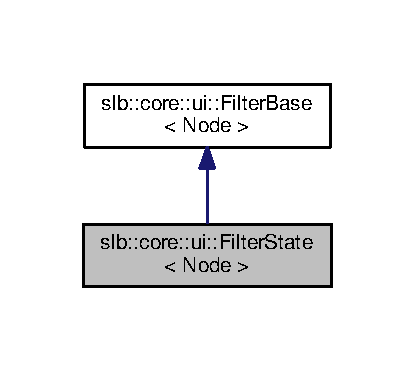
\includegraphics[width=199pt]{structslb_1_1core_1_1ui_1_1FilterState__inherit__graph}
\end{center}
\end{figure}


Collaboration diagram for slb\+:\+:core\+:\+:ui\+:\+:Filter\+State$<$ Node $>$\+:\nopagebreak
\begin{figure}[H]
\begin{center}
\leavevmode
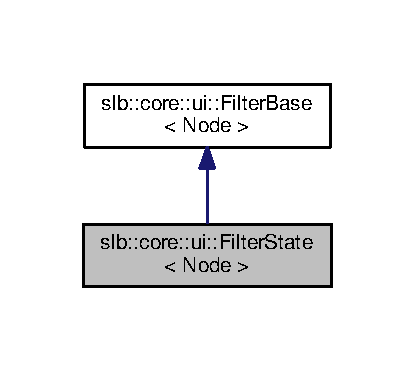
\includegraphics[width=199pt]{structslb_1_1core_1_1ui_1_1FilterState__coll__graph}
\end{center}
\end{figure}
\subsubsection*{Public Types}
\begin{DoxyCompactItemize}
\item 
using \hyperlink{structslb_1_1core_1_1ui_1_1FilterState_ae0f6db7b501ec68290584480ef9cab78}{Event} = typename \hyperlink{structslb_1_1core_1_1ui_1_1FilterBase}{Filter\+Base}$<$ Node $>$\+::\hyperlink{structslb_1_1core_1_1ui_1_1FilterBase_a4cf70d819855984dc0e15a036e8b8a14}{Event}\hypertarget{structslb_1_1core_1_1ui_1_1FilterState_ae0f6db7b501ec68290584480ef9cab78}{}\label{structslb_1_1core_1_1ui_1_1FilterState_ae0f6db7b501ec68290584480ef9cab78}

\begin{DoxyCompactList}\small\item\em The type representing an event generated by the search algorithm. \end{DoxyCompactList}\item 
using \hyperlink{structslb_1_1core_1_1ui_1_1FilterState_a832a02468e2d15393c1937a33988073b}{State\+Shared\+Ptr} = typename \hyperlink{structslb_1_1core_1_1ui_1_1FilterBase}{Filter\+Base}$<$ Node $>$\+::\hyperlink{structslb_1_1core_1_1ui_1_1FilterState_a832a02468e2d15393c1937a33988073b}{State\+Shared\+Ptr}\hypertarget{structslb_1_1core_1_1ui_1_1FilterState_a832a02468e2d15393c1937a33988073b}{}\label{structslb_1_1core_1_1ui_1_1FilterState_a832a02468e2d15393c1937a33988073b}

\begin{DoxyCompactList}\small\item\em Smart pointer to state type representing the domain. \end{DoxyCompactList}\end{DoxyCompactItemize}
\subsubsection*{Public Member Functions}
\begin{DoxyCompactItemize}
\item 
virtual bool \hyperlink{structslb_1_1core_1_1ui_1_1FilterState_abacffaaa5ed7700394e99ede2744323c}{in} (const \hyperlink{structslb_1_1core_1_1ui_1_1FilterBase_a4cf70d819855984dc0e15a036e8b8a14}{Event} \&e) const 
\begin{DoxyCompactList}\small\item\em Determines whether the given event is not filtered out. \end{DoxyCompactList}\item 
void \hyperlink{structslb_1_1core_1_1ui_1_1FilterState_a6d8d4b243aae17bf8de0e021cd8978d0}{add} (const \hyperlink{structslb_1_1core_1_1ui_1_1FilterState_a832a02468e2d15393c1937a33988073b}{State\+Shared\+Ptr} state)
\begin{DoxyCompactList}\small\item\em Adds a state to the list of the states of interest. \end{DoxyCompactList}\item 
void \hyperlink{structslb_1_1core_1_1ui_1_1FilterState_a0f0e9f69414535fb3df1287970cfd6b9}{set} (const \hyperlink{structslb_1_1core_1_1ui_1_1FilterState_a832a02468e2d15393c1937a33988073b}{State\+Shared\+Ptr} state)
\begin{DoxyCompactList}\small\item\em Resets the list of the states of interest to contain only the given state. \end{DoxyCompactList}\item 
void \hyperlink{structslb_1_1core_1_1ui_1_1FilterState_a7039b0a4edf4a7d45ea61c0bbcea5b33}{reset} ()\hypertarget{structslb_1_1core_1_1ui_1_1FilterState_a7039b0a4edf4a7d45ea61c0bbcea5b33}{}\label{structslb_1_1core_1_1ui_1_1FilterState_a7039b0a4edf4a7d45ea61c0bbcea5b33}

\begin{DoxyCompactList}\small\item\em Empties the list of the states of interest. \end{DoxyCompactList}\end{DoxyCompactItemize}
\subsubsection*{Private Attributes}
\begin{DoxyCompactItemize}
\item 
std\+::vector$<$ \hyperlink{structslb_1_1core_1_1ui_1_1FilterState_a832a02468e2d15393c1937a33988073b}{State\+Shared\+Ptr} $>$ \hyperlink{structslb_1_1core_1_1ui_1_1FilterState_a4a0d6995c62160fb54b0adbb8ac9f366}{states\+\_\+}\hypertarget{structslb_1_1core_1_1ui_1_1FilterState_a4a0d6995c62160fb54b0adbb8ac9f366}{}\label{structslb_1_1core_1_1ui_1_1FilterState_a4a0d6995c62160fb54b0adbb8ac9f366}

\begin{DoxyCompactList}\small\item\em The list of the states of interest that should not be filtered out. \end{DoxyCompactList}\end{DoxyCompactItemize}


\subsubsection{Detailed Description}
\subsubsection*{template$<$class Node$>$\\*
struct slb\+::core\+::ui\+::\+Filter\+State$<$ Node $>$}

Filters by leaving only events related to chosen states. When the list of states is empty, no events are filtered out. 


\begin{DoxyTemplParams}{Template Parameters}
{\em Node} & The search node type. \\
\hline
\end{DoxyTemplParams}


Definition at line 74 of file filters.\+h.



\subsubsection{Member Function Documentation}
\index{slb\+::core\+::ui\+::\+Filter\+State@{slb\+::core\+::ui\+::\+Filter\+State}!add@{add}}
\index{add@{add}!slb\+::core\+::ui\+::\+Filter\+State@{slb\+::core\+::ui\+::\+Filter\+State}}
\paragraph[{\texorpdfstring{add(const State\+Shared\+Ptr state)}{add(const StateSharedPtr state)}}]{\setlength{\rightskip}{0pt plus 5cm}template$<$class Node$>$ void {\bf slb\+::core\+::ui\+::\+Filter\+State}$<$ Node $>$\+::add (
\begin{DoxyParamCaption}
\item[{const {\bf State\+Shared\+Ptr}}]{state}
\end{DoxyParamCaption}
)\hspace{0.3cm}{\ttfamily [inline]}}\hypertarget{structslb_1_1core_1_1ui_1_1FilterState_a6d8d4b243aae17bf8de0e021cd8978d0}{}\label{structslb_1_1core_1_1ui_1_1FilterState_a6d8d4b243aae17bf8de0e021cd8978d0}


Adds a state to the list of the states of interest. 


\begin{DoxyParams}{Parameters}
{\em state} & Smart pointer to the state of interest. \\
\hline
\end{DoxyParams}


Definition at line 91 of file filters.\+h.

\index{slb\+::core\+::ui\+::\+Filter\+State@{slb\+::core\+::ui\+::\+Filter\+State}!in@{in}}
\index{in@{in}!slb\+::core\+::ui\+::\+Filter\+State@{slb\+::core\+::ui\+::\+Filter\+State}}
\paragraph[{\texorpdfstring{in(const Event \&e) const }{in(const Event &e) const }}]{\setlength{\rightskip}{0pt plus 5cm}template$<$class Node$>$ virtual bool {\bf slb\+::core\+::ui\+::\+Filter\+State}$<$ Node $>$\+::in (
\begin{DoxyParamCaption}
\item[{const {\bf Event} \&}]{e}
\end{DoxyParamCaption}
) const\hspace{0.3cm}{\ttfamily [inline]}, {\ttfamily [virtual]}}\hypertarget{structslb_1_1core_1_1ui_1_1FilterState_abacffaaa5ed7700394e99ede2744323c}{}\label{structslb_1_1core_1_1ui_1_1FilterState_abacffaaa5ed7700394e99ede2744323c}


Determines whether the given event is not filtered out. 


\begin{DoxyParams}{Parameters}
{\em e} & The event of interest. \\
\hline
\end{DoxyParams}
\begin{DoxyReturn}{Returns}
{\ttfamily true} if the given event is not filtered out. 
\end{DoxyReturn}


Implements \hyperlink{structslb_1_1core_1_1ui_1_1FilterBase_af89dfa7be8a61ad95f688b43f40379ad}{slb\+::core\+::ui\+::\+Filter\+Base$<$ Node $>$}.



Definition at line 84 of file filters.\+h.

\index{slb\+::core\+::ui\+::\+Filter\+State@{slb\+::core\+::ui\+::\+Filter\+State}!set@{set}}
\index{set@{set}!slb\+::core\+::ui\+::\+Filter\+State@{slb\+::core\+::ui\+::\+Filter\+State}}
\paragraph[{\texorpdfstring{set(const State\+Shared\+Ptr state)}{set(const StateSharedPtr state)}}]{\setlength{\rightskip}{0pt plus 5cm}template$<$class Node$>$ void {\bf slb\+::core\+::ui\+::\+Filter\+State}$<$ Node $>$\+::set (
\begin{DoxyParamCaption}
\item[{const {\bf State\+Shared\+Ptr}}]{state}
\end{DoxyParamCaption}
)\hspace{0.3cm}{\ttfamily [inline]}}\hypertarget{structslb_1_1core_1_1ui_1_1FilterState_a0f0e9f69414535fb3df1287970cfd6b9}{}\label{structslb_1_1core_1_1ui_1_1FilterState_a0f0e9f69414535fb3df1287970cfd6b9}


Resets the list of the states of interest to contain only the given state. 


\begin{DoxyParams}{Parameters}
{\em state} & Smart pointer to the state of interest. \\
\hline
\end{DoxyParams}


Definition at line 96 of file filters.\+h.



The documentation for this struct was generated from the following file\+:\begin{DoxyCompactItemize}
\item 
core/user\+\_\+interface/\hyperlink{filters_8h}{filters.\+h}\end{DoxyCompactItemize}

\hypertarget{structslb_1_1core_1_1ui_1_1Form}{}\subsection{slb\+:\+:core\+:\+:ui\+:\+:Form Struct Reference}
\label{structslb_1_1core_1_1ui_1_1Form}\index{slb\+::core\+::ui\+::\+Form@{slb\+::core\+::ui\+::\+Form}}


A simple form for ncurses. Forms that come with {\ttfamily ncurses} cannot be put in pad windows.  




{\ttfamily \#include $<$form.\+h$>$}

\subsubsection*{Public Member Functions}
\begin{DoxyCompactItemize}
\item 
bool \hyperlink{structslb_1_1core_1_1ui_1_1Form_a8620608c03f10da64add6ff57a264667}{empty} () const 
\begin{DoxyCompactList}\small\item\em Returns {\ttfamily true} if the form does not contain any fields and {\ttfamily false} otherwise. \end{DoxyCompactList}\item 
bool \hyperlink{structslb_1_1core_1_1ui_1_1Form_a96b694556d31b41fad4ed52b13fcddec}{handle} (int keystate, int keycode)
\begin{DoxyCompactList}\small\item\em Passes the given key that was pressed to the active field for handling. Handles by itself keys for moving between the fields. \end{DoxyCompactList}\item 
void \hyperlink{structslb_1_1core_1_1ui_1_1Form_a55bfdb477b8698608fbe320d820e7f3d}{display} () const \hypertarget{structslb_1_1core_1_1ui_1_1Form_a55bfdb477b8698608fbe320d820e7f3d}{}\label{structslb_1_1core_1_1ui_1_1Form_a55bfdb477b8698608fbe320d820e7f3d}

\begin{DoxyCompactList}\small\item\em Displays the form with all its fields. \end{DoxyCompactList}\item 
const std\+::string \& \hyperlink{structslb_1_1core_1_1ui_1_1Form_a2a0da97a1f8a4b19489022417f3b8dfa}{get} (int fieldN) const 
\begin{DoxyCompactList}\small\item\em Returns the contents of the active field. \end{DoxyCompactList}\item 
void \hyperlink{structslb_1_1core_1_1ui_1_1Form_a2d33c87a993c6bf4e2a95e6dcd0d1ac3}{add\+Field} (const \hyperlink{structslb_1_1core_1_1ui_1_1EditField}{Edit\+Field} \&f)
\begin{DoxyCompactList}\small\item\em Adds the given field to the form. \end{DoxyCompactList}\item 
void \hyperlink{structslb_1_1core_1_1ui_1_1Form_a503e6e9b06c01543741f05ba11056253}{set} (const std\+::string \&s)
\begin{DoxyCompactList}\small\item\em Sets the contents of the active field. \end{DoxyCompactList}\end{DoxyCompactItemize}
\subsubsection*{Private Attributes}
\begin{DoxyCompactItemize}
\item 
std\+::vector$<$ \hyperlink{structslb_1_1core_1_1ui_1_1EditField}{Edit\+Field} $>$ \hyperlink{structslb_1_1core_1_1ui_1_1Form_a271aab2a6797907d901475bbd4d7c02b}{fields\+\_\+}\hypertarget{structslb_1_1core_1_1ui_1_1Form_a271aab2a6797907d901475bbd4d7c02b}{}\label{structslb_1_1core_1_1ui_1_1Form_a271aab2a6797907d901475bbd4d7c02b}

\begin{DoxyCompactList}\small\item\em Fields the constitute the form. \end{DoxyCompactList}\item 
int \hyperlink{structslb_1_1core_1_1ui_1_1Form_ac5a6500f7dd89f3bd9c50b76d2af8771}{active\+\_\+} \{\}\hypertarget{structslb_1_1core_1_1ui_1_1Form_ac5a6500f7dd89f3bd9c50b76d2af8771}{}\label{structslb_1_1core_1_1ui_1_1Form_ac5a6500f7dd89f3bd9c50b76d2af8771}

\begin{DoxyCompactList}\small\item\em Index into {\ttfamily fields\+\_\+} indicating the active field. \end{DoxyCompactList}\end{DoxyCompactItemize}


\subsubsection{Detailed Description}
A simple form for ncurses. Forms that come with {\ttfamily ncurses} cannot be put in pad windows. 

Definition at line 142 of file form.\+h.



\subsubsection{Member Function Documentation}
\index{slb\+::core\+::ui\+::\+Form@{slb\+::core\+::ui\+::\+Form}!add\+Field@{add\+Field}}
\index{add\+Field@{add\+Field}!slb\+::core\+::ui\+::\+Form@{slb\+::core\+::ui\+::\+Form}}
\paragraph[{\texorpdfstring{add\+Field(const Edit\+Field \&f)}{addField(const EditField &f)}}]{\setlength{\rightskip}{0pt plus 5cm}void slb\+::core\+::ui\+::\+Form\+::add\+Field (
\begin{DoxyParamCaption}
\item[{const {\bf Edit\+Field} \&}]{f}
\end{DoxyParamCaption}
)\hspace{0.3cm}{\ttfamily [inline]}}\hypertarget{structslb_1_1core_1_1ui_1_1Form_a2d33c87a993c6bf4e2a95e6dcd0d1ac3}{}\label{structslb_1_1core_1_1ui_1_1Form_a2d33c87a993c6bf4e2a95e6dcd0d1ac3}


Adds the given field to the form. 


\begin{DoxyParams}{Parameters}
{\em f} & The field to be added. \\
\hline
\end{DoxyParams}


Definition at line 175 of file form.\+h.

\index{slb\+::core\+::ui\+::\+Form@{slb\+::core\+::ui\+::\+Form}!empty@{empty}}
\index{empty@{empty}!slb\+::core\+::ui\+::\+Form@{slb\+::core\+::ui\+::\+Form}}
\paragraph[{\texorpdfstring{empty() const }{empty() const }}]{\setlength{\rightskip}{0pt plus 5cm}bool slb\+::core\+::ui\+::\+Form\+::empty (
\begin{DoxyParamCaption}
{}
\end{DoxyParamCaption}
) const\hspace{0.3cm}{\ttfamily [inline]}}\hypertarget{structslb_1_1core_1_1ui_1_1Form_a8620608c03f10da64add6ff57a264667}{}\label{structslb_1_1core_1_1ui_1_1Form_a8620608c03f10da64add6ff57a264667}


Returns {\ttfamily true} if the form does not contain any fields and {\ttfamily false} otherwise. 

\begin{DoxyReturn}{Returns}
{\ttfamily true} if the form does not contain any fields and {\ttfamily false} otherwise. 
\end{DoxyReturn}


Definition at line 147 of file form.\+h.

\index{slb\+::core\+::ui\+::\+Form@{slb\+::core\+::ui\+::\+Form}!get@{get}}
\index{get@{get}!slb\+::core\+::ui\+::\+Form@{slb\+::core\+::ui\+::\+Form}}
\paragraph[{\texorpdfstring{get(int field\+N) const }{get(int fieldN) const }}]{\setlength{\rightskip}{0pt plus 5cm}const std\+::string\& slb\+::core\+::ui\+::\+Form\+::get (
\begin{DoxyParamCaption}
\item[{int}]{fieldN}
\end{DoxyParamCaption}
) const\hspace{0.3cm}{\ttfamily [inline]}}\hypertarget{structslb_1_1core_1_1ui_1_1Form_a2a0da97a1f8a4b19489022417f3b8dfa}{}\label{structslb_1_1core_1_1ui_1_1Form_a2a0da97a1f8a4b19489022417f3b8dfa}


Returns the contents of the active field. 

\begin{DoxyReturn}{Returns}
The contents of the active field. 
\end{DoxyReturn}


Definition at line 171 of file form.\+h.

\index{slb\+::core\+::ui\+::\+Form@{slb\+::core\+::ui\+::\+Form}!handle@{handle}}
\index{handle@{handle}!slb\+::core\+::ui\+::\+Form@{slb\+::core\+::ui\+::\+Form}}
\paragraph[{\texorpdfstring{handle(int keystate, int keycode)}{handle(int keystate, int keycode)}}]{\setlength{\rightskip}{0pt plus 5cm}bool slb\+::core\+::ui\+::\+Form\+::handle (
\begin{DoxyParamCaption}
\item[{int}]{keystate, }
\item[{int}]{keycode}
\end{DoxyParamCaption}
)\hspace{0.3cm}{\ttfamily [inline]}}\hypertarget{structslb_1_1core_1_1ui_1_1Form_a96b694556d31b41fad4ed52b13fcddec}{}\label{structslb_1_1core_1_1ui_1_1Form_a96b694556d31b41fad4ed52b13fcddec}


Passes the given key that was pressed to the active field for handling. Handles by itself keys for moving between the fields. 


\begin{DoxyParams}{Parameters}
{\em keystate} & The key group. \\
\hline
{\em keycode} & The key. \\
\hline
\end{DoxyParams}
\begin{DoxyReturn}{Returns}
{\ttfamily true} if the key was handled by the form and {\ttfamily false} otherwise. 
\end{DoxyReturn}


Definition at line 155 of file form.\+h.

\index{slb\+::core\+::ui\+::\+Form@{slb\+::core\+::ui\+::\+Form}!set@{set}}
\index{set@{set}!slb\+::core\+::ui\+::\+Form@{slb\+::core\+::ui\+::\+Form}}
\paragraph[{\texorpdfstring{set(const std\+::string \&s)}{set(const std::string &s)}}]{\setlength{\rightskip}{0pt plus 5cm}void slb\+::core\+::ui\+::\+Form\+::set (
\begin{DoxyParamCaption}
\item[{const std\+::string \&}]{s}
\end{DoxyParamCaption}
)\hspace{0.3cm}{\ttfamily [inline]}}\hypertarget{structslb_1_1core_1_1ui_1_1Form_a503e6e9b06c01543741f05ba11056253}{}\label{structslb_1_1core_1_1ui_1_1Form_a503e6e9b06c01543741f05ba11056253}


Sets the contents of the active field. 


\begin{DoxyParams}{Parameters}
{\em s} & New contents. \\
\hline
\end{DoxyParams}


Definition at line 179 of file form.\+h.



The documentation for this struct was generated from the following file\+:\begin{DoxyCompactItemize}
\item 
core/user\+\_\+interface/\hyperlink{form_8h}{form.\+h}\end{DoxyCompactItemize}

\hypertarget{structslb_1_1ext_1_1heuristic_1_1differential_1_1Furthest}{}\subsection{slb\+:\+:ext\+:\+:heuristic\+:\+:differential\+:\+:Furthest Struct Reference}
\label{structslb_1_1ext_1_1heuristic_1_1differential_1_1Furthest}\index{slb\+::ext\+::heuristic\+::differential\+::\+Furthest@{slb\+::ext\+::heuristic\+::differential\+::\+Furthest}}


Type for the furthest placement policy.  




{\ttfamily \#include $<$differential.\+h$>$}



\subsubsection{Detailed Description}
Type for the furthest placement policy. 

Definition at line 38 of file differential.\+h.



The documentation for this struct was generated from the following file\+:\begin{DoxyCompactItemize}
\item 
extensions/heuristics/differential/\hyperlink{differential_8h}{differential.\+h}\end{DoxyCompactItemize}

\hypertarget{structslb_1_1ext_1_1domain_1_1pancake_1_1GapHeuristic}{}\subsection{slb\+:\+:ext\+:\+:domain\+:\+:pancake\+:\+:Gap\+Heuristic Struct Reference}
\label{structslb_1_1ext_1_1domain_1_1pancake_1_1GapHeuristic}\index{slb\+::ext\+::domain\+::pancake\+::\+Gap\+Heuristic@{slb\+::ext\+::domain\+::pancake\+::\+Gap\+Heuristic}}


Functor for computing the gap heuristic to the goal state with ordered pancakes.  




{\ttfamily \#include $<$pancake.\+h$>$}

\subsubsection*{Public Member Functions}
\begin{DoxyCompactItemize}
\item 
\hyperlink{structslb_1_1ext_1_1domain_1_1pancake_1_1GapHeuristic_ad9d47e11fc855f38ca746629887c43eb}{Gap\+Heuristic} (const \hyperlink{structslb_1_1ext_1_1domain_1_1pancake_1_1Pancake}{Pancake} \&)\hypertarget{structslb_1_1ext_1_1domain_1_1pancake_1_1GapHeuristic_ad9d47e11fc855f38ca746629887c43eb}{}\label{structslb_1_1ext_1_1domain_1_1pancake_1_1GapHeuristic_ad9d47e11fc855f38ca746629887c43eb}

\begin{DoxyCompactList}\small\item\em The constructor. \end{DoxyCompactList}\item 
int \hyperlink{structslb_1_1ext_1_1domain_1_1pancake_1_1GapHeuristic_aec4b2f568f9f2ba7ebf866ea8b455af4}{operator()} (const \hyperlink{structslb_1_1ext_1_1domain_1_1pancake_1_1Pancake}{Pancake} \&s) const 
\begin{DoxyCompactList}\small\item\em The call operator. Computes the gap heuristic from the given state to the goal state with ordered pancakes. \end{DoxyCompactList}\end{DoxyCompactItemize}


\subsubsection{Detailed Description}
Functor for computing the gap heuristic to the goal state with ordered pancakes. 

Definition at line 228 of file pancake.\+h.



\subsubsection{Member Function Documentation}
\index{slb\+::ext\+::domain\+::pancake\+::\+Gap\+Heuristic@{slb\+::ext\+::domain\+::pancake\+::\+Gap\+Heuristic}!operator()@{operator()}}
\index{operator()@{operator()}!slb\+::ext\+::domain\+::pancake\+::\+Gap\+Heuristic@{slb\+::ext\+::domain\+::pancake\+::\+Gap\+Heuristic}}
\paragraph[{\texorpdfstring{operator()(const Pancake \&s) const }{operator()(const Pancake &s) const }}]{\setlength{\rightskip}{0pt plus 5cm}int slb\+::ext\+::domain\+::pancake\+::\+Gap\+Heuristic\+::operator() (
\begin{DoxyParamCaption}
\item[{const {\bf Pancake} \&}]{s}
\end{DoxyParamCaption}
) const\hspace{0.3cm}{\ttfamily [inline]}}\hypertarget{structslb_1_1ext_1_1domain_1_1pancake_1_1GapHeuristic_aec4b2f568f9f2ba7ebf866ea8b455af4}{}\label{structslb_1_1ext_1_1domain_1_1pancake_1_1GapHeuristic_aec4b2f568f9f2ba7ebf866ea8b455af4}


The call operator. Computes the gap heuristic from the given state to the goal state with ordered pancakes. 


\begin{DoxyParams}{Parameters}
{\em s} & The state from which the heuristic value is needed. \\
\hline
\end{DoxyParams}
\begin{DoxyReturn}{Returns}
The gap heuristic from {\ttfamily s} to the goal state with ordered pancakes. 
\end{DoxyReturn}


Definition at line 237 of file pancake.\+h.



The documentation for this struct was generated from the following file\+:\begin{DoxyCompactItemize}
\item 
extensions/domains/\hyperlink{pancake_8h}{pancake.\+h}\end{DoxyCompactItemize}

\hypertarget{structslb_1_1ext_1_1domain_1_1pancake_1_1GapHeuristicToGoal}{}\subsection{slb\+:\+:ext\+:\+:domain\+:\+:pancake\+:\+:Gap\+Heuristic\+To\+Goal Struct Reference}
\label{structslb_1_1ext_1_1domain_1_1pancake_1_1GapHeuristicToGoal}\index{slb\+::ext\+::domain\+::pancake\+::\+Gap\+Heuristic\+To\+Goal@{slb\+::ext\+::domain\+::pancake\+::\+Gap\+Heuristic\+To\+Goal}}


Functor for computing the gap heuristic to the given goal state.  




{\ttfamily \#include $<$pancake.\+h$>$}



Collaboration diagram for slb\+:\+:ext\+:\+:domain\+:\+:pancake\+:\+:Gap\+Heuristic\+To\+Goal\+:\nopagebreak
\begin{figure}[H]
\begin{center}
\leavevmode
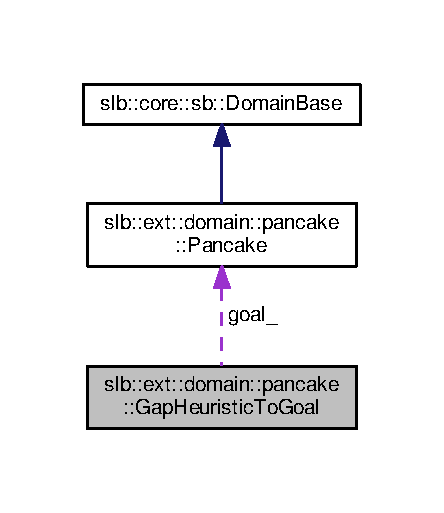
\includegraphics[width=213pt]{structslb_1_1ext_1_1domain_1_1pancake_1_1GapHeuristicToGoal__coll__graph}
\end{center}
\end{figure}
\subsubsection*{Public Member Functions}
\begin{DoxyCompactItemize}
\item 
\hyperlink{structslb_1_1ext_1_1domain_1_1pancake_1_1GapHeuristicToGoal_a7cc1d87a1d31d85e9e1d284b8d054dfa}{Gap\+Heuristic\+To\+Goal} (const \hyperlink{structslb_1_1ext_1_1domain_1_1pancake_1_1Pancake}{Pancake} \&goal)
\begin{DoxyCompactList}\small\item\em The constructor. \end{DoxyCompactList}\item 
int \hyperlink{structslb_1_1ext_1_1domain_1_1pancake_1_1GapHeuristicToGoal_a6c1729a3aa1f8aacb5ab614e87ed8cb9}{operator()} (const \hyperlink{structslb_1_1ext_1_1domain_1_1pancake_1_1Pancake}{Pancake} \&s) const 
\begin{DoxyCompactList}\small\item\em The call operator. Computes the gap heuristic from the given state to the given goal state. \end{DoxyCompactList}\end{DoxyCompactItemize}
\subsubsection*{Private Attributes}
\begin{DoxyCompactItemize}
\item 
const \hyperlink{structslb_1_1ext_1_1domain_1_1pancake_1_1Pancake}{Pancake} \& \hyperlink{structslb_1_1ext_1_1domain_1_1pancake_1_1GapHeuristicToGoal_a49c66f8a7df7b89718d1be057b7f8fed}{goal\+\_\+}\hypertarget{structslb_1_1ext_1_1domain_1_1pancake_1_1GapHeuristicToGoal_a49c66f8a7df7b89718d1be057b7f8fed}{}\label{structslb_1_1ext_1_1domain_1_1pancake_1_1GapHeuristicToGoal_a49c66f8a7df7b89718d1be057b7f8fed}

\begin{DoxyCompactList}\small\item\em The goal state. \end{DoxyCompactList}\end{DoxyCompactItemize}


\subsubsection{Detailed Description}
Functor for computing the gap heuristic to the given goal state. 

Definition at line 258 of file pancake.\+h.



\subsubsection{Constructor \& Destructor Documentation}
\index{slb\+::ext\+::domain\+::pancake\+::\+Gap\+Heuristic\+To\+Goal@{slb\+::ext\+::domain\+::pancake\+::\+Gap\+Heuristic\+To\+Goal}!Gap\+Heuristic\+To\+Goal@{Gap\+Heuristic\+To\+Goal}}
\index{Gap\+Heuristic\+To\+Goal@{Gap\+Heuristic\+To\+Goal}!slb\+::ext\+::domain\+::pancake\+::\+Gap\+Heuristic\+To\+Goal@{slb\+::ext\+::domain\+::pancake\+::\+Gap\+Heuristic\+To\+Goal}}
\paragraph[{\texorpdfstring{Gap\+Heuristic\+To\+Goal(const Pancake \&goal)}{GapHeuristicToGoal(const Pancake &goal)}}]{\setlength{\rightskip}{0pt plus 5cm}slb\+::ext\+::domain\+::pancake\+::\+Gap\+Heuristic\+To\+Goal\+::\+Gap\+Heuristic\+To\+Goal (
\begin{DoxyParamCaption}
\item[{const {\bf Pancake} \&}]{goal}
\end{DoxyParamCaption}
)\hspace{0.3cm}{\ttfamily [inline]}}\hypertarget{structslb_1_1ext_1_1domain_1_1pancake_1_1GapHeuristicToGoal_a7cc1d87a1d31d85e9e1d284b8d054dfa}{}\label{structslb_1_1ext_1_1domain_1_1pancake_1_1GapHeuristicToGoal_a7cc1d87a1d31d85e9e1d284b8d054dfa}


The constructor. 


\begin{DoxyParams}{Parameters}
{\em goal} & The goal state. \\
\hline
\end{DoxyParams}


Definition at line 261 of file pancake.\+h.



\subsubsection{Member Function Documentation}
\index{slb\+::ext\+::domain\+::pancake\+::\+Gap\+Heuristic\+To\+Goal@{slb\+::ext\+::domain\+::pancake\+::\+Gap\+Heuristic\+To\+Goal}!operator()@{operator()}}
\index{operator()@{operator()}!slb\+::ext\+::domain\+::pancake\+::\+Gap\+Heuristic\+To\+Goal@{slb\+::ext\+::domain\+::pancake\+::\+Gap\+Heuristic\+To\+Goal}}
\paragraph[{\texorpdfstring{operator()(const Pancake \&s) const }{operator()(const Pancake &s) const }}]{\setlength{\rightskip}{0pt plus 5cm}int slb\+::ext\+::domain\+::pancake\+::\+Gap\+Heuristic\+To\+Goal\+::operator() (
\begin{DoxyParamCaption}
\item[{const {\bf Pancake} \&}]{s}
\end{DoxyParamCaption}
) const\hspace{0.3cm}{\ttfamily [inline]}}\hypertarget{structslb_1_1ext_1_1domain_1_1pancake_1_1GapHeuristicToGoal_a6c1729a3aa1f8aacb5ab614e87ed8cb9}{}\label{structslb_1_1ext_1_1domain_1_1pancake_1_1GapHeuristicToGoal_a6c1729a3aa1f8aacb5ab614e87ed8cb9}


The call operator. Computes the gap heuristic from the given state to the given goal state. 


\begin{DoxyParams}{Parameters}
{\em s} & The state from which the heuristic value is needed. \\
\hline
\end{DoxyParams}
\begin{DoxyReturn}{Returns}
The gap heuristic from {\ttfamily s} to {\ttfamily goal\+\_\+}. 
\end{DoxyReturn}


Definition at line 267 of file pancake.\+h.



The documentation for this struct was generated from the following file\+:\begin{DoxyCompactItemize}
\item 
extensions/domains/\hyperlink{pancake_8h}{pancake.\+h}\end{DoxyCompactItemize}

\hypertarget{structslb_1_1ext_1_1event_1_1Generated}{}\subsection{slb\+:\+:ext\+:\+:event\+:\+:Generated$<$ Node $>$ Struct Template Reference}
\label{structslb_1_1ext_1_1event_1_1Generated}\index{slb\+::ext\+::event\+::\+Generated$<$ Node $>$@{slb\+::ext\+::event\+::\+Generated$<$ Node $>$}}


Event that visualizes node generation.  




{\ttfamily \#include $<$events.\+h$>$}



Inheritance diagram for slb\+:\+:ext\+:\+:event\+:\+:Generated$<$ Node $>$\+:\nopagebreak
\begin{figure}[H]
\begin{center}
\leavevmode
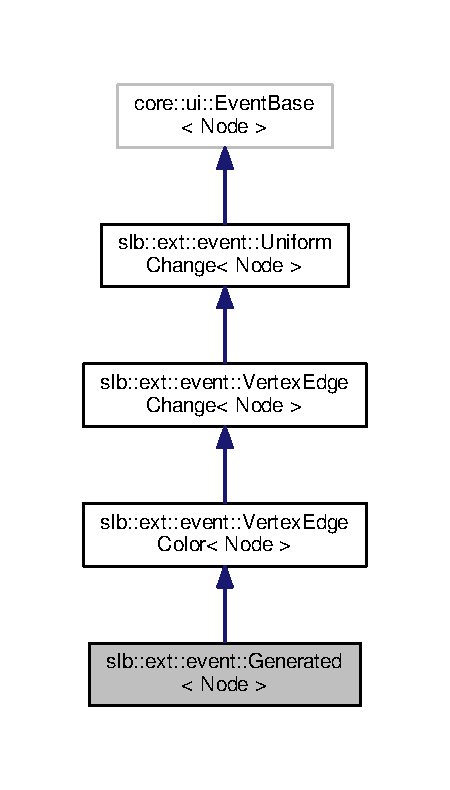
\includegraphics[width=216pt]{structslb_1_1ext_1_1event_1_1Generated__inherit__graph}
\end{center}
\end{figure}


Collaboration diagram for slb\+:\+:ext\+:\+:event\+:\+:Generated$<$ Node $>$\+:\nopagebreak
\begin{figure}[H]
\begin{center}
\leavevmode
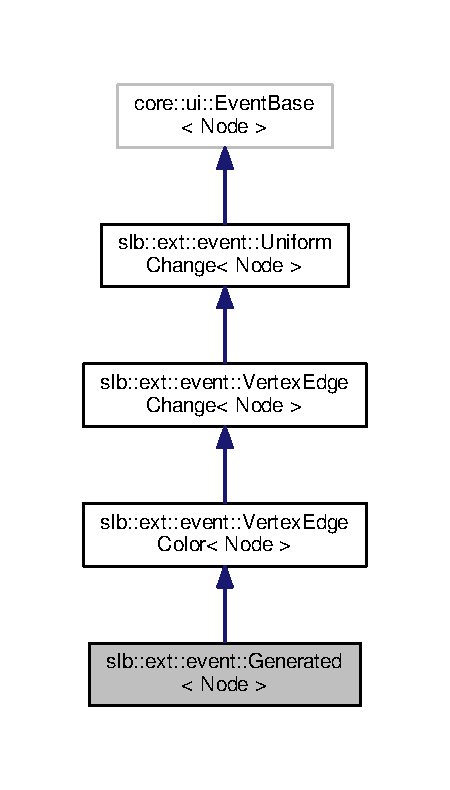
\includegraphics[width=216pt]{structslb_1_1ext_1_1event_1_1Generated__coll__graph}
\end{center}
\end{figure}
\subsubsection*{Private Member Functions}
\begin{DoxyCompactItemize}
\item 
virtual Color \hyperlink{structslb_1_1ext_1_1event_1_1Generated_ae7d0033ee8badedc3057c363ecd00650}{color} () const override
\begin{DoxyCompactList}\small\item\em Returns the new color of both the vertex of the state graph corresponding to the state associated with the event and the edge by which the search algorithm arrived to this state. \end{DoxyCompactList}\item 
std\+::string \hyperlink{structslb_1_1ext_1_1event_1_1Generated_ad2bf6cf56f05c805b19dfa1ca73b5ae6}{event\+Str} () const override
\begin{DoxyCompactList}\small\item\em Returns the string describing the event. This string is displayed in the log window. \end{DoxyCompactList}\end{DoxyCompactItemize}
\subsubsection*{Additional Inherited Members}


\subsubsection{Detailed Description}
\subsubsection*{template$<$class Node = S\+L\+B\+\_\+\+N\+O\+DE$>$\\*
struct slb\+::ext\+::event\+::\+Generated$<$ Node $>$}

Event that visualizes node generation. 


\begin{DoxyTemplParams}{Template Parameters}
{\em Node} & The search node type. \\
\hline
\end{DoxyTemplParams}


Definition at line 74 of file events.\+h.



\subsubsection{Member Function Documentation}
\index{slb\+::ext\+::event\+::\+Generated@{slb\+::ext\+::event\+::\+Generated}!color@{color}}
\index{color@{color}!slb\+::ext\+::event\+::\+Generated@{slb\+::ext\+::event\+::\+Generated}}
\paragraph[{\texorpdfstring{color() const override}{color() const override}}]{\setlength{\rightskip}{0pt plus 5cm}template$<$class Node  = S\+L\+B\+\_\+\+N\+O\+DE$>$ virtual Color {\bf slb\+::ext\+::event\+::\+Generated}$<$ Node $>$\+::color (
\begin{DoxyParamCaption}
{}
\end{DoxyParamCaption}
) const\hspace{0.3cm}{\ttfamily [inline]}, {\ttfamily [override]}, {\ttfamily [private]}, {\ttfamily [virtual]}}\hypertarget{structslb_1_1ext_1_1event_1_1Generated_ae7d0033ee8badedc3057c363ecd00650}{}\label{structslb_1_1ext_1_1event_1_1Generated_ae7d0033ee8badedc3057c363ecd00650}


Returns the new color of both the vertex of the state graph corresponding to the state associated with the event and the edge by which the search algorithm arrived to this state. 

\begin{DoxyReturn}{Returns}
The new color of both the vertex of the state graph corresponding to the state associated with the event and the edge by which the search algorithm arrived to this state. 
\end{DoxyReturn}


Implements \hyperlink{structslb_1_1ext_1_1event_1_1VertexEdgeColor_ac5d0c212a4e807eccbc7082b8834ef77}{slb\+::ext\+::event\+::\+Vertex\+Edge\+Color$<$ Node $>$}.



Definition at line 85 of file events.\+h.

\index{slb\+::ext\+::event\+::\+Generated@{slb\+::ext\+::event\+::\+Generated}!event\+Str@{event\+Str}}
\index{event\+Str@{event\+Str}!slb\+::ext\+::event\+::\+Generated@{slb\+::ext\+::event\+::\+Generated}}
\paragraph[{\texorpdfstring{event\+Str() const override}{eventStr() const override}}]{\setlength{\rightskip}{0pt plus 5cm}template$<$class Node  = S\+L\+B\+\_\+\+N\+O\+DE$>$ std\+::string {\bf slb\+::ext\+::event\+::\+Generated}$<$ Node $>$\+::event\+Str (
\begin{DoxyParamCaption}
{}
\end{DoxyParamCaption}
) const\hspace{0.3cm}{\ttfamily [inline]}, {\ttfamily [override]}, {\ttfamily [private]}}\hypertarget{structslb_1_1ext_1_1event_1_1Generated_ad2bf6cf56f05c805b19dfa1ca73b5ae6}{}\label{structslb_1_1ext_1_1event_1_1Generated_ad2bf6cf56f05c805b19dfa1ca73b5ae6}


Returns the string describing the event. This string is displayed in the log window. 

\begin{DoxyReturn}{Returns}
The string describing the event. 
\end{DoxyReturn}


Definition at line 90 of file events.\+h.



The documentation for this struct was generated from the following file\+:\begin{DoxyCompactItemize}
\item 
extensions/events/\hyperlink{events_8h}{events.\+h}\end{DoxyCompactItemize}

\hypertarget{structslb_1_1core_1_1ui_1_1Graphics}{}\subsection{slb\+:\+:core\+:\+:ui\+:\+:Graphics Struct Reference}
\label{structslb_1_1core_1_1ui_1_1Graphics}\index{slb\+::core\+::ui\+::\+Graphics@{slb\+::core\+::ui\+::\+Graphics}}


Objects of this class hold all the information needed for drawing.  




{\ttfamily \#include $<$graphics\+\_\+object.\+h$>$}

\subsubsection*{Public Member Functions}
\begin{DoxyCompactItemize}
\item 
\hyperlink{structslb_1_1core_1_1ui_1_1Graphics_affbe27c97d1598cda401b993b22cf214}{Graphics} ()\hypertarget{structslb_1_1core_1_1ui_1_1Graphics_affbe27c97d1598cda401b993b22cf214}{}\label{structslb_1_1core_1_1ui_1_1Graphics_affbe27c97d1598cda401b993b22cf214}

\begin{DoxyCompactList}\small\item\em Creates the window, initializes the surface and the drawing context. \end{DoxyCompactList}\item 
\hyperlink{structslb_1_1core_1_1ui_1_1Graphics_aa571f74e8c3f74506db24e4f6eb04135}{$\sim$\+Graphics} ()\hypertarget{structslb_1_1core_1_1ui_1_1Graphics_aa571f74e8c3f74506db24e4f6eb04135}{}\label{structslb_1_1core_1_1ui_1_1Graphics_aa571f74e8c3f74506db24e4f6eb04135}

\begin{DoxyCompactList}\small\item\em Frees the resources. \end{DoxyCompactList}\item 
void \hyperlink{structslb_1_1core_1_1ui_1_1Graphics_ac04ff16245079a00c7832a77e7332e82}{scale} ()\hypertarget{structslb_1_1core_1_1ui_1_1Graphics_ac04ff16245079a00c7832a77e7332e82}{}\label{structslb_1_1core_1_1ui_1_1Graphics_ac04ff16245079a00c7832a77e7332e82}

\begin{DoxyCompactList}\small\item\em Restores the scale to 1.\+0. \end{DoxyCompactList}\item 
void \hyperlink{structslb_1_1core_1_1ui_1_1Graphics_a71571b540232fcec048f4636e2743f05}{translate} ()\hypertarget{structslb_1_1core_1_1ui_1_1Graphics_a71571b540232fcec048f4636e2743f05}{}\label{structslb_1_1core_1_1ui_1_1Graphics_a71571b540232fcec048f4636e2743f05}

\begin{DoxyCompactList}\small\item\em Restores the user coordinates (0,0) to device coordinate (0,0) \end{DoxyCompactList}\item 
void \hyperlink{structslb_1_1core_1_1ui_1_1Graphics_aa45a87f7bfd22656864992c5f8f7b63d}{restore} ()\hypertarget{structslb_1_1core_1_1ui_1_1Graphics_aa45a87f7bfd22656864992c5f8f7b63d}{}\label{structslb_1_1core_1_1ui_1_1Graphics_aa45a87f7bfd22656864992c5f8f7b63d}

\begin{DoxyCompactList}\small\item\em Restores both the scale to 1.\+0 and translation to make the origin same in both user and device coordinates. \end{DoxyCompactList}\item 
void \hyperlink{structslb_1_1core_1_1ui_1_1Graphics_a6f285650256346fdd36fe7cb3b562cbb}{scale} (double factor)
\begin{DoxyCompactList}\small\item\em Scales the graphical representation of the (partial) domain graph. \end{DoxyCompactList}\item 
void \hyperlink{structslb_1_1core_1_1ui_1_1Graphics_afdba5da7dc3fd6e716bd3a464212404a}{update\+Window\+Size} (int x, int y)
\begin{DoxyCompactList}\small\item\em Update the size of the window and the drawing surface. \end{DoxyCompactList}\end{DoxyCompactItemize}
\subsubsection*{Public Attributes}
\begin{DoxyCompactItemize}
\item 
int \hyperlink{structslb_1_1core_1_1ui_1_1Graphics_a7be3cfcd2b96c069f314f77ca413a012}{window\+X\+Size} = 500\hypertarget{structslb_1_1core_1_1ui_1_1Graphics_a7be3cfcd2b96c069f314f77ca413a012}{}\label{structslb_1_1core_1_1ui_1_1Graphics_a7be3cfcd2b96c069f314f77ca413a012}

\begin{DoxyCompactList}\small\item\em the x-\/dimension of the window \end{DoxyCompactList}\item 
int \hyperlink{structslb_1_1core_1_1ui_1_1Graphics_ad361367c824b2d9cccd9d8ee76320ab6}{window\+Y\+Size} = 500\hypertarget{structslb_1_1core_1_1ui_1_1Graphics_ad361367c824b2d9cccd9d8ee76320ab6}{}\label{structslb_1_1core_1_1ui_1_1Graphics_ad361367c824b2d9cccd9d8ee76320ab6}

\begin{DoxyCompactList}\small\item\em the y-\/dimension of the window \end{DoxyCompactList}\item 
int \hyperlink{structslb_1_1core_1_1ui_1_1Graphics_ae02ff446ffd8215e15aaf79c96c99ad3}{sizeX} = 500\hypertarget{structslb_1_1core_1_1ui_1_1Graphics_ae02ff446ffd8215e15aaf79c96c99ad3}{}\label{structslb_1_1core_1_1ui_1_1Graphics_ae02ff446ffd8215e15aaf79c96c99ad3}

\begin{DoxyCompactList}\small\item\em the x-\/dimension of the drawing with the current scaling factor. \end{DoxyCompactList}\item 
int \hyperlink{structslb_1_1core_1_1ui_1_1Graphics_a5fb9d2d27de9c4f99bdd46e80b580d72}{sizeY} = 500\hypertarget{structslb_1_1core_1_1ui_1_1Graphics_a5fb9d2d27de9c4f99bdd46e80b580d72}{}\label{structslb_1_1core_1_1ui_1_1Graphics_a5fb9d2d27de9c4f99bdd46e80b580d72}

\begin{DoxyCompactList}\small\item\em the y-\/dimension of the drawing with the current scaling factor. \end{DoxyCompactList}\item 
double \hyperlink{structslb_1_1core_1_1ui_1_1Graphics_a9fd508fc1907290c21608fdcd03918b4}{margin} = 1.\+0\hypertarget{structslb_1_1core_1_1ui_1_1Graphics_a9fd508fc1907290c21608fdcd03918b4}{}\label{structslb_1_1core_1_1ui_1_1Graphics_a9fd508fc1907290c21608fdcd03918b4}

\begin{DoxyCompactList}\small\item\em The factor of window width/height added to the drawing surface compared to the window size on each side. For example, margin==1.\+0 means that the dimensions of the drawing surface are three times larger than the corresponding dimensions of the window. \end{DoxyCompactList}\item 
double \hyperlink{structslb_1_1core_1_1ui_1_1Graphics_a5992d0a3c4f220c962a900e43e5abd8e}{scale\+Factor} = 1.\+0\hypertarget{structslb_1_1core_1_1ui_1_1Graphics_a5992d0a3c4f220c962a900e43e5abd8e}{}\label{structslb_1_1core_1_1ui_1_1Graphics_a5992d0a3c4f220c962a900e43e5abd8e}

\begin{DoxyCompactList}\small\item\em Current scaling factor. \end{DoxyCompactList}\end{DoxyCompactItemize}
\begin{Indent}{\bf The information needed for drawing.}\par
{\em Please refer to \href{https://www.cairographics.org/Xlib/}{\tt https\+://www.\+cairographics.\+org/\+Xlib/} for more information. }\begin{DoxyCompactItemize}
\item 
Display $\ast$ {\bfseries display} \{\}\hypertarget{structslb_1_1core_1_1ui_1_1Graphics_aaee15e1382e9b404705f0b3095f01f25}{}\label{structslb_1_1core_1_1ui_1_1Graphics_aaee15e1382e9b404705f0b3095f01f25}

\item 
Window {\bfseries w}\hypertarget{structslb_1_1core_1_1ui_1_1Graphics_a0144f51c16d4fc2870602739c59a71da}{}\label{structslb_1_1core_1_1ui_1_1Graphics_a0144f51c16d4fc2870602739c59a71da}

\item 
Window {\bfseries root}\hypertarget{structslb_1_1core_1_1ui_1_1Graphics_a22def7a1a7f4f53c6899614d9673675f}{}\label{structslb_1_1core_1_1ui_1_1Graphics_a22def7a1a7f4f53c6899614d9673675f}

\item 
cairo\+\_\+surface\+\_\+t $\ast$ {\bfseries surface} \{\}\hypertarget{structslb_1_1core_1_1ui_1_1Graphics_a4ba46f3015dcfe2ecb869f8d297e69e2}{}\label{structslb_1_1core_1_1ui_1_1Graphics_a4ba46f3015dcfe2ecb869f8d297e69e2}

\item 
cairo\+\_\+t $\ast$ {\bfseries cr} \{\}\hypertarget{structslb_1_1core_1_1ui_1_1Graphics_adb908af9559c1c941aa26bba80786dcf}{}\label{structslb_1_1core_1_1ui_1_1Graphics_adb908af9559c1c941aa26bba80786dcf}

\end{DoxyCompactItemize}
\end{Indent}
\begin{Indent}{\bf Top-\/left corner of the drawing.}\par
{\em Device coordinates of the top-\/left corner of the drawing surface at the time of the last re-\/drawing. }\begin{DoxyCompactItemize}
\item 
double {\bfseries zeroX} = 0.\+0\hypertarget{structslb_1_1core_1_1ui_1_1Graphics_a24963adcd37c5cd0e8bfc5f0ba7f16f4}{}\label{structslb_1_1core_1_1ui_1_1Graphics_a24963adcd37c5cd0e8bfc5f0ba7f16f4}

\item 
double {\bfseries zeroY} = 0.\+0\hypertarget{structslb_1_1core_1_1ui_1_1Graphics_ab3f726f711f87251530feba2e0b99dff}{}\label{structslb_1_1core_1_1ui_1_1Graphics_ab3f726f711f87251530feba2e0b99dff}

\end{DoxyCompactItemize}
\end{Indent}


\subsubsection{Detailed Description}
Objects of this class hold all the information needed for drawing. 

Definition at line 13 of file graphics\+\_\+object.\+h.



\subsubsection{Member Function Documentation}
\index{slb\+::core\+::ui\+::\+Graphics@{slb\+::core\+::ui\+::\+Graphics}!scale@{scale}}
\index{scale@{scale}!slb\+::core\+::ui\+::\+Graphics@{slb\+::core\+::ui\+::\+Graphics}}
\paragraph[{\texorpdfstring{scale(double factor)}{scale(double factor)}}]{\setlength{\rightskip}{0pt plus 5cm}void slb\+::core\+::ui\+::\+Graphics\+::scale (
\begin{DoxyParamCaption}
\item[{double}]{factor}
\end{DoxyParamCaption}
)\hspace{0.3cm}{\ttfamily [inline]}}\hypertarget{structslb_1_1core_1_1ui_1_1Graphics_a6f285650256346fdd36fe7cb3b562cbb}{}\label{structslb_1_1core_1_1ui_1_1Graphics_a6f285650256346fdd36fe7cb3b562cbb}


Scales the graphical representation of the (partial) domain graph. 


\begin{DoxyParams}{Parameters}
{\em factor} & The scaling factor. \\
\hline
\end{DoxyParams}


Definition at line 60 of file graphics\+\_\+object.\+h.

\index{slb\+::core\+::ui\+::\+Graphics@{slb\+::core\+::ui\+::\+Graphics}!update\+Window\+Size@{update\+Window\+Size}}
\index{update\+Window\+Size@{update\+Window\+Size}!slb\+::core\+::ui\+::\+Graphics@{slb\+::core\+::ui\+::\+Graphics}}
\paragraph[{\texorpdfstring{update\+Window\+Size(int x, int y)}{updateWindowSize(int x, int y)}}]{\setlength{\rightskip}{0pt plus 5cm}void slb\+::core\+::ui\+::\+Graphics\+::update\+Window\+Size (
\begin{DoxyParamCaption}
\item[{int}]{x, }
\item[{int}]{y}
\end{DoxyParamCaption}
)\hspace{0.3cm}{\ttfamily [inline]}}\hypertarget{structslb_1_1core_1_1ui_1_1Graphics_afdba5da7dc3fd6e716bd3a464212404a}{}\label{structslb_1_1core_1_1ui_1_1Graphics_afdba5da7dc3fd6e716bd3a464212404a}


Update the size of the window and the drawing surface. 


\begin{DoxyParams}{Parameters}
{\em x} & New x-\/dimension of the window. \\
\hline
{\em y} & New y-\/dimension of the window. \\
\hline
\end{DoxyParams}


Definition at line 79 of file graphics\+\_\+object.\+h.



The documentation for this struct was generated from the following file\+:\begin{DoxyCompactItemize}
\item 
core/user\+\_\+interface/\hyperlink{graphics__object_8h}{graphics\+\_\+object.\+h}\end{DoxyCompactItemize}

\hypertarget{structslb_1_1ext_1_1policy_1_1openList_1_1GreaterPriority__SmallF__LargeG}{}\subsection{slb\+:\+:ext\+:\+:policy\+:\+:open\+List\+:\+:Greater\+Priority\+\_\+\+Small\+F\+\_\+\+LargeG$<$ Key\+Type $>$ Struct Template Reference}
\label{structslb_1_1ext_1_1policy_1_1openList_1_1GreaterPriority__SmallF__LargeG}\index{slb\+::ext\+::policy\+::open\+List\+::\+Greater\+Priority\+\_\+\+Small\+F\+\_\+\+Large\+G$<$ Key\+Type $>$@{slb\+::ext\+::policy\+::open\+List\+::\+Greater\+Priority\+\_\+\+Small\+F\+\_\+\+Large\+G$<$ Key\+Type $>$}}


Functor that compares keys based on f-\/value and breaks ties in favor of larger g-\/value.  




{\ttfamily \#include $<$open\+\_\+list.\+h$>$}

\subsubsection*{Public Member Functions}
\begin{DoxyCompactItemize}
\item 
bool \hyperlink{structslb_1_1ext_1_1policy_1_1openList_1_1GreaterPriority__SmallF__LargeG_ae6322cd3c71786a3d1299991e7a3d175}{operator()} (const Key\+Type \&lhs, const Key\+Type \&rhs)
\begin{DoxyCompactList}\small\item\em Compares two keys. \end{DoxyCompactList}\end{DoxyCompactItemize}


\subsubsection{Detailed Description}
\subsubsection*{template$<$class Key\+Type$>$\\*
struct slb\+::ext\+::policy\+::open\+List\+::\+Greater\+Priority\+\_\+\+Small\+F\+\_\+\+Large\+G$<$ Key\+Type $>$}

Functor that compares keys based on f-\/value and breaks ties in favor of larger g-\/value. 


\begin{DoxyTemplParams}{Template Parameters}
{\em Key\+Type} & The key type. \\
\hline
\end{DoxyTemplParams}

\begin{DoxyParams}{Parameters}
{\em lhs} & The left-\/hand side key in the comparison. \\
\hline
{\em rhs} & The right-\/hand side key in the comparison. \\
\hline
\end{DoxyParams}
\begin{DoxyReturn}{Returns}
{\ttfamily true} if {\ttfamily lhs} is higher priority than {\ttfamily rhs} and {\ttfamily false} otherwise. 
\end{DoxyReturn}


Definition at line 75 of file open\+\_\+list.\+h.



\subsubsection{Member Function Documentation}
\index{slb\+::ext\+::policy\+::open\+List\+::\+Greater\+Priority\+\_\+\+Small\+F\+\_\+\+LargeG@{slb\+::ext\+::policy\+::open\+List\+::\+Greater\+Priority\+\_\+\+Small\+F\+\_\+\+LargeG}!operator()@{operator()}}
\index{operator()@{operator()}!slb\+::ext\+::policy\+::open\+List\+::\+Greater\+Priority\+\_\+\+Small\+F\+\_\+\+LargeG@{slb\+::ext\+::policy\+::open\+List\+::\+Greater\+Priority\+\_\+\+Small\+F\+\_\+\+LargeG}}
\paragraph[{\texorpdfstring{operator()(const Key\+Type \&lhs, const Key\+Type \&rhs)}{operator()(const KeyType &lhs, const KeyType &rhs)}}]{\setlength{\rightskip}{0pt plus 5cm}template$<$class Key\+Type $>$ bool {\bf slb\+::ext\+::policy\+::open\+List\+::\+Greater\+Priority\+\_\+\+Small\+F\+\_\+\+LargeG}$<$ Key\+Type $>$\+::operator() (
\begin{DoxyParamCaption}
\item[{const Key\+Type \&}]{lhs, }
\item[{const Key\+Type \&}]{rhs}
\end{DoxyParamCaption}
)\hspace{0.3cm}{\ttfamily [inline]}}\hypertarget{structslb_1_1ext_1_1policy_1_1openList_1_1GreaterPriority__SmallF__LargeG_ae6322cd3c71786a3d1299991e7a3d175}{}\label{structslb_1_1ext_1_1policy_1_1openList_1_1GreaterPriority__SmallF__LargeG_ae6322cd3c71786a3d1299991e7a3d175}


Compares two keys. 


\begin{DoxyParams}{Parameters}
{\em lhs} & First key. \\
\hline
{\em rhs} & Second key. \\
\hline
\end{DoxyParams}
\begin{DoxyReturn}{Returns}
{\ttfamily true} if {\ttfamily lhs} precedes {\ttfamily rhs} and {\ttfamily false} otherwise. 
\end{DoxyReturn}


Definition at line 80 of file open\+\_\+list.\+h.



The documentation for this struct was generated from the following file\+:\begin{DoxyCompactItemize}
\item 
extensions/shared\+\_\+policies/\hyperlink{open__list_8h}{open\+\_\+list.\+h}\end{DoxyCompactItemize}

\hypertarget{structslb_1_1ext_1_1policy_1_1openList_1_1GreaterPriority__SmallG}{}\subsection{slb\+:\+:ext\+:\+:policy\+:\+:open\+List\+:\+:Greater\+Priority\+\_\+\+SmallG$<$ Key\+Type $>$ Struct Template Reference}
\label{structslb_1_1ext_1_1policy_1_1openList_1_1GreaterPriority__SmallG}\index{slb\+::ext\+::policy\+::open\+List\+::\+Greater\+Priority\+\_\+\+Small\+G$<$ Key\+Type $>$@{slb\+::ext\+::policy\+::open\+List\+::\+Greater\+Priority\+\_\+\+Small\+G$<$ Key\+Type $>$}}


Functor that compares keys based on g-\/value and prioritizes in favor of a smaller g-\/value.  




{\ttfamily \#include $<$open\+\_\+list.\+h$>$}

\subsubsection*{Public Member Functions}
\begin{DoxyCompactItemize}
\item 
bool \hyperlink{structslb_1_1ext_1_1policy_1_1openList_1_1GreaterPriority__SmallG_a5bfd65b87aff6817a1294a5ec488f115}{operator()} (const Key\+Type \&lhs, const Key\+Type \&rhs)
\begin{DoxyCompactList}\small\item\em Compares two keys. \end{DoxyCompactList}\end{DoxyCompactItemize}


\subsubsection{Detailed Description}
\subsubsection*{template$<$class Key\+Type$>$\\*
struct slb\+::ext\+::policy\+::open\+List\+::\+Greater\+Priority\+\_\+\+Small\+G$<$ Key\+Type $>$}

Functor that compares keys based on g-\/value and prioritizes in favor of a smaller g-\/value. 


\begin{DoxyTemplParams}{Template Parameters}
{\em Key\+Type} & The key type. \\
\hline
\end{DoxyTemplParams}

\begin{DoxyParams}{Parameters}
{\em lhs} & The left-\/hand side key in the comparison. \\
\hline
{\em rhs} & The right-\/hand side key in the comparison. \\
\hline
\end{DoxyParams}
\begin{DoxyReturn}{Returns}
{\ttfamily true} if {\ttfamily lhs} is higher priority than {\ttfamily rhs} and {\ttfamily false} otherwise. 
\end{DoxyReturn}


Definition at line 96 of file open\+\_\+list.\+h.



\subsubsection{Member Function Documentation}
\index{slb\+::ext\+::policy\+::open\+List\+::\+Greater\+Priority\+\_\+\+SmallG@{slb\+::ext\+::policy\+::open\+List\+::\+Greater\+Priority\+\_\+\+SmallG}!operator()@{operator()}}
\index{operator()@{operator()}!slb\+::ext\+::policy\+::open\+List\+::\+Greater\+Priority\+\_\+\+SmallG@{slb\+::ext\+::policy\+::open\+List\+::\+Greater\+Priority\+\_\+\+SmallG}}
\paragraph[{\texorpdfstring{operator()(const Key\+Type \&lhs, const Key\+Type \&rhs)}{operator()(const KeyType &lhs, const KeyType &rhs)}}]{\setlength{\rightskip}{0pt plus 5cm}template$<$class Key\+Type $>$ bool {\bf slb\+::ext\+::policy\+::open\+List\+::\+Greater\+Priority\+\_\+\+SmallG}$<$ Key\+Type $>$\+::operator() (
\begin{DoxyParamCaption}
\item[{const Key\+Type \&}]{lhs, }
\item[{const Key\+Type \&}]{rhs}
\end{DoxyParamCaption}
)\hspace{0.3cm}{\ttfamily [inline]}}\hypertarget{structslb_1_1ext_1_1policy_1_1openList_1_1GreaterPriority__SmallG_a5bfd65b87aff6817a1294a5ec488f115}{}\label{structslb_1_1ext_1_1policy_1_1openList_1_1GreaterPriority__SmallG_a5bfd65b87aff6817a1294a5ec488f115}


Compares two keys. 


\begin{DoxyParams}{Parameters}
{\em lhs} & First key. \\
\hline
{\em rhs} & Second key. \\
\hline
\end{DoxyParams}
\begin{DoxyReturn}{Returns}
{\ttfamily true} if {\ttfamily lhs} precedes {\ttfamily rhs} and {\ttfamily false} otherwise. 
\end{DoxyReturn}


Definition at line 101 of file open\+\_\+list.\+h.



The documentation for this struct was generated from the following file\+:\begin{DoxyCompactItemize}
\item 
extensions/shared\+\_\+policies/\hyperlink{open__list_8h}{open\+\_\+list.\+h}\end{DoxyCompactItemize}

\hypertarget{structslb_1_1ext_1_1explicit__space_1_1Grid}{}\subsection{slb\+:\+:ext\+:\+:explicit\+\_\+space\+:\+:Grid$<$ Cost\+Type\+\_\+ $>$ Struct Template Reference}
\label{structslb_1_1ext_1_1explicit__space_1_1Grid}\index{slb\+::ext\+::explicit\+\_\+space\+::\+Grid$<$ Cost\+Type\+\_\+ $>$@{slb\+::ext\+::explicit\+\_\+space\+::\+Grid$<$ Cost\+Type\+\_\+ $>$}}


The type for 4 or 8-\/connected grid explicit domain.  




{\ttfamily \#include $<$grid.\+h$>$}

\subsubsection*{Classes}
\begin{DoxyCompactItemize}
\item 
struct \hyperlink{structslb_1_1ext_1_1explicit__space_1_1Grid_1_1StateIterator}{State\+Iterator}
\begin{DoxyCompactList}\small\item\em The state iterator type. \end{DoxyCompactList}\end{DoxyCompactItemize}
\subsubsection*{Public Types}
\begin{DoxyCompactItemize}
\item 
using \hyperlink{structslb_1_1ext_1_1explicit__space_1_1Grid_a800819a8f2c96bf76dd9d36c18760815}{Cost\+Type} = Cost\+Type\+\_\+\hypertarget{structslb_1_1ext_1_1explicit__space_1_1Grid_a800819a8f2c96bf76dd9d36c18760815}{}\label{structslb_1_1ext_1_1explicit__space_1_1Grid_a800819a8f2c96bf76dd9d36c18760815}

\begin{DoxyCompactList}\small\item\em Type for action cost in the search domain. \end{DoxyCompactList}\item 
using \hyperlink{structslb_1_1ext_1_1explicit__space_1_1Grid_a2b2125f1774b299ea7f0f9f21d967fde}{Location} = int\hypertarget{structslb_1_1ext_1_1explicit__space_1_1Grid_a2b2125f1774b299ea7f0f9f21d967fde}{}\label{structslb_1_1ext_1_1explicit__space_1_1Grid_a2b2125f1774b299ea7f0f9f21d967fde}

\begin{DoxyCompactList}\small\item\em The type used internally by this explicit space to represent a state. To distinguish this state type from the state type used by search algorithms, we call this state type {\ttfamily location}. \end{DoxyCompactList}\item 
using \hyperlink{structslb_1_1ext_1_1explicit__space_1_1Grid_a75c71647e997ddb8f8f442d4e173d962}{Location\+Iterator} = \hyperlink{structslb_1_1core_1_1util_1_1IndexIterator}{core\+::util\+::\+Index\+Iterator}$<$ std\+::vector$<$ bool $>$, \hyperlink{namespaceslb_1_1core_1_1util_a5692b540118495a35ebae95fb8b80790}{core\+::util\+::\+Vector\+Skip\+Const\+Iterator}$<$ std\+::vector$<$ bool $>$$>$$>$\hypertarget{structslb_1_1ext_1_1explicit__space_1_1Grid_a75c71647e997ddb8f8f442d4e173d962}{}\label{structslb_1_1ext_1_1explicit__space_1_1Grid_a75c71647e997ddb8f8f442d4e173d962}

\begin{DoxyCompactList}\small\item\em The type of iterator over passable locations. \end{DoxyCompactList}\end{DoxyCompactItemize}
\subsubsection*{Public Member Functions}
\begin{DoxyCompactItemize}
\item 
\hyperlink{structslb_1_1ext_1_1explicit__space_1_1Grid_a0f99334c0b664c55ed0b2a22a29d650a}{Grid} (std\+::string file\+Name)
\begin{DoxyCompactList}\small\item\em Initializes the grid based on the contents of the given file. \end{DoxyCompactList}\item 
\hyperlink{structslb_1_1ext_1_1explicit__space_1_1Grid_a2b2125f1774b299ea7f0f9f21d967fde}{Location} \hyperlink{structslb_1_1ext_1_1explicit__space_1_1Grid_a55b2b168ae56fb372304763478c4ca4b}{location} (int r, int c) const 
\begin{DoxyCompactList}\small\item\em Returns location based on row and column in the grid. \end{DoxyCompactList}\item 
int \hyperlink{structslb_1_1ext_1_1explicit__space_1_1Grid_acddf0950aadbbf55bc83f23b7ef4ed66}{row} (\hyperlink{structslb_1_1ext_1_1explicit__space_1_1Grid_a2b2125f1774b299ea7f0f9f21d967fde}{Location} loc) const 
\begin{DoxyCompactList}\small\item\em Returns row based on location. \end{DoxyCompactList}\item 
int \hyperlink{structslb_1_1ext_1_1explicit__space_1_1Grid_a0f91db20cb68595560b16235468289b9}{column} (\hyperlink{structslb_1_1ext_1_1explicit__space_1_1Grid_a2b2125f1774b299ea7f0f9f21d967fde}{Location} loc) const 
\begin{DoxyCompactList}\small\item\em Returns column based on location. \end{DoxyCompactList}\item 
bool \hyperlink{structslb_1_1ext_1_1explicit__space_1_1Grid_a574a12701271635e52714e53e3e88edd}{passable} (int r, int c) const 
\begin{DoxyCompactList}\small\item\em Returns {\ttfamily true} if the location {\ttfamily }(r,c) is passable and {\ttfamily false} otherwise. \end{DoxyCompactList}\item 
bool \hyperlink{structslb_1_1ext_1_1explicit__space_1_1Grid_afc920bb4a27c239b20b16efb0e745401}{passable} (\hyperlink{structslb_1_1ext_1_1explicit__space_1_1Grid_a2b2125f1774b299ea7f0f9f21d967fde}{Location} loc) const 
\begin{DoxyCompactList}\small\item\em Returns {\ttfamily true} if the location {\ttfamily loc} is passable and {\ttfamily false} otherwise. \end{DoxyCompactList}\item 
{\footnotesize template$<$class Neighbor $>$ }\\std\+::vector$<$ Neighbor $>$ \hyperlink{structslb_1_1ext_1_1explicit__space_1_1Grid_ab526a9f0eb4d12dd7ee93b3ff9359bbf}{neighbors} (int loc) const 
\begin{DoxyCompactList}\small\item\em Computes the set of neighbors of the given location. \end{DoxyCompactList}\item 
\hyperlink{structslb_1_1ext_1_1explicit__space_1_1Grid_a2b2125f1774b299ea7f0f9f21d967fde}{Location} \hyperlink{structslb_1_1ext_1_1explicit__space_1_1Grid_a6ff6ce8a97bfe218a3fc4625c3c71b34}{location} (const std\+::string str) const 
\begin{DoxyCompactList}\small\item\em Returns a location based on the given string, e.\+g. \char`\"{}\mbox{[}105, 400\mbox{]}\char`\"{}. \end{DoxyCompactList}\item 
\hyperlink{structslb_1_1ext_1_1explicit__space_1_1Grid_a2b2125f1774b299ea7f0f9f21d967fde}{Location} \hyperlink{structslb_1_1ext_1_1explicit__space_1_1Grid_a1d5777e338c0f81783994f11a594f4a9}{random} () const 
\begin{DoxyCompactList}\small\item\em Returns a random location. \end{DoxyCompactList}\item 
\hyperlink{structslb_1_1ext_1_1explicit__space_1_1Grid_a2b2125f1774b299ea7f0f9f21d967fde}{Location} \hyperlink{structslb_1_1ext_1_1explicit__space_1_1Grid_a10058dd5412f488eac980d89e2256cb9}{default\+Location} () const 
\begin{DoxyCompactList}\small\item\em Returns the default location. \end{DoxyCompactList}\item 
void \hyperlink{structslb_1_1ext_1_1explicit__space_1_1Grid_acaa4f99a13ede903d5a4426b8167d8b2}{visual\+Location} (\hyperlink{structslb_1_1ext_1_1explicit__space_1_1Grid_a2b2125f1774b299ea7f0f9f21d967fde}{Location} loc, double \&x, double \&y) const 
\begin{DoxyCompactList}\small\item\em Fills out the coordinates for the vertex representing the state. \end{DoxyCompactList}\item 
\hyperlink{structslb_1_1ext_1_1explicit__space_1_1Grid_a800819a8f2c96bf76dd9d36c18760815}{Cost\+Type} \hyperlink{structslb_1_1ext_1_1explicit__space_1_1Grid_a174a24dbd770989f5f6374e618b50010}{manhattan} (\hyperlink{structslb_1_1ext_1_1explicit__space_1_1Grid_a2b2125f1774b299ea7f0f9f21d967fde}{Location} \hyperlink{structslb_1_1ext_1_1explicit__space_1_1Grid_a55b2b168ae56fb372304763478c4ca4b}{location}, \hyperlink{structslb_1_1ext_1_1explicit__space_1_1Grid_a2b2125f1774b299ea7f0f9f21d967fde}{Location} goal) const 
\begin{DoxyCompactList}\small\item\em Computes the Manhattan distance heuristic. \end{DoxyCompactList}\item 
\hyperlink{structslb_1_1ext_1_1explicit__space_1_1Grid_a800819a8f2c96bf76dd9d36c18760815}{Cost\+Type} \hyperlink{structslb_1_1ext_1_1explicit__space_1_1Grid_a51ed15da62b0362554a0b4471176a9e0}{octile} (\hyperlink{structslb_1_1ext_1_1explicit__space_1_1Grid_a2b2125f1774b299ea7f0f9f21d967fde}{Location} \hyperlink{structslb_1_1ext_1_1explicit__space_1_1Grid_a55b2b168ae56fb372304763478c4ca4b}{location}, \hyperlink{structslb_1_1ext_1_1explicit__space_1_1Grid_a2b2125f1774b299ea7f0f9f21d967fde}{Location} goal) const 
\begin{DoxyCompactList}\small\item\em Computes the octile distance heuristic. \end{DoxyCompactList}\item 
std\+::string \hyperlink{structslb_1_1ext_1_1explicit__space_1_1Grid_a69148d3f12f7f933bf94af0cdc7f217a}{location\+Short\+Str} (\hyperlink{structslb_1_1ext_1_1explicit__space_1_1Grid_a2b2125f1774b299ea7f0f9f21d967fde}{Location} \hyperlink{structslb_1_1ext_1_1explicit__space_1_1Grid_a55b2b168ae56fb372304763478c4ca4b}{location}) const 
\begin{DoxyCompactList}\small\item\em Returns the string representation of the given location. \end{DoxyCompactList}\item 
std\+::string \hyperlink{structslb_1_1ext_1_1explicit__space_1_1Grid_a6a4048decbe8d61178986f4ae09884f9}{location\+Str} (\hyperlink{structslb_1_1ext_1_1explicit__space_1_1Grid_a2b2125f1774b299ea7f0f9f21d967fde}{Location} \hyperlink{structslb_1_1ext_1_1explicit__space_1_1Grid_a55b2b168ae56fb372304763478c4ca4b}{location}) const 
\begin{DoxyCompactList}\small\item\em Returns the string representation of the given location. \end{DoxyCompactList}\item 
int \hyperlink{structslb_1_1ext_1_1explicit__space_1_1Grid_ae1dfa66a8c9f25eb20fa2baf8552876a}{raw\+Size} () const 
\begin{DoxyCompactList}\small\item\em Return the size of \hyperlink{structslb_1_1ext_1_1explicit__space_1_1Grid_aecb404c6bc75e985ee31a4fef89433d2}{v\+\_\+}. \end{DoxyCompactList}\end{DoxyCompactItemize}
\subsubsection*{Private Member Functions}
\begin{DoxyCompactItemize}
\item 
{\footnotesize template$<$class Neighbor $>$ }\\void \hyperlink{structslb_1_1ext_1_1explicit__space_1_1Grid_a804425c4377ce2933be9f3ea655dd940}{add\+Neighbor} (std\+::vector$<$ Neighbor $>$ \&res, \hyperlink{structslb_1_1ext_1_1explicit__space_1_1Grid_a2b2125f1774b299ea7f0f9f21d967fde}{Location} n, bool diagonal\+Flag=false) const 
\begin{DoxyCompactList}\small\item\em Adds a neighbor corresponding to the given location to the given set of neighbors. \end{DoxyCompactList}\item 
\hyperlink{structslb_1_1ext_1_1explicit__space_1_1Grid_a75c71647e997ddb8f8f442d4e173d962}{Location\+Iterator} {\bfseries location\+Iterator} ()\hypertarget{structslb_1_1ext_1_1explicit__space_1_1Grid_a0136e082c52c7d3c7334b64fd69f4985}{}\label{structslb_1_1ext_1_1explicit__space_1_1Grid_a0136e082c52c7d3c7334b64fd69f4985}

\item 
{\footnotesize template$<$class Explicit\+State $>$ }\\\hyperlink{structslb_1_1ext_1_1explicit__space_1_1Grid_1_1StateIterator}{State\+Iterator}$<$ \hyperlink{structslb_1_1core_1_1sb_1_1ExplicitState}{Explicit\+State} $>$ {\bfseries begin\+State\+Iterator} ()\hypertarget{structslb_1_1ext_1_1explicit__space_1_1Grid_ac672b9b4974011f4c10243a9c42e5e5e}{}\label{structslb_1_1ext_1_1explicit__space_1_1Grid_ac672b9b4974011f4c10243a9c42e5e5e}

\item 
{\footnotesize template$<$class Explicit\+State $>$ }\\\hyperlink{structslb_1_1ext_1_1explicit__space_1_1Grid_1_1StateIterator}{State\+Iterator}$<$ \hyperlink{structslb_1_1core_1_1sb_1_1ExplicitState}{Explicit\+State} $>$ {\bfseries end\+State\+Iterator} ()\hypertarget{structslb_1_1ext_1_1explicit__space_1_1Grid_a6652bd758225247b7bbc741461d4bf67}{}\label{structslb_1_1ext_1_1explicit__space_1_1Grid_a6652bd758225247b7bbc741461d4bf67}

\end{DoxyCompactItemize}
\subsubsection*{Private Attributes}
\begin{DoxyCompactItemize}
\item 
std\+::vector$<$ bool $>$ \hyperlink{structslb_1_1ext_1_1explicit__space_1_1Grid_aecb404c6bc75e985ee31a4fef89433d2}{v\+\_\+}\hypertarget{structslb_1_1ext_1_1explicit__space_1_1Grid_aecb404c6bc75e985ee31a4fef89433d2}{}\label{structslb_1_1ext_1_1explicit__space_1_1Grid_aecb404c6bc75e985ee31a4fef89433d2}

\begin{DoxyCompactList}\small\item\em The encoding of the map. {\ttfamily true} stands for passable, {\ttfamily false} stands for impassable. \end{DoxyCompactList}\item 
int \hyperlink{structslb_1_1ext_1_1explicit__space_1_1Grid_af4f7a157ef85745b866d3fc938a1f311}{width\+\_\+}\hypertarget{structslb_1_1ext_1_1explicit__space_1_1Grid_af4f7a157ef85745b866d3fc938a1f311}{}\label{structslb_1_1ext_1_1explicit__space_1_1Grid_af4f7a157ef85745b866d3fc938a1f311}

\begin{DoxyCompactList}\small\item\em Map\textquotesingle{}s width (i.\+e. number of columns). \end{DoxyCompactList}\item 
int \hyperlink{structslb_1_1ext_1_1explicit__space_1_1Grid_ac8b358b686d1e2524164d2d3979471ec}{height\+\_\+}\hypertarget{structslb_1_1ext_1_1explicit__space_1_1Grid_ac8b358b686d1e2524164d2d3979471ec}{}\label{structslb_1_1ext_1_1explicit__space_1_1Grid_ac8b358b686d1e2524164d2d3979471ec}

\begin{DoxyCompactList}\small\item\em Map\textquotesingle{}s height (i.\+e. number of rows). \end{DoxyCompactList}\item 
bool \hyperlink{structslb_1_1ext_1_1explicit__space_1_1Grid_a73bb43d1f3c9c7202a0e01753baaefd9}{octile\+Flag\+\_\+}\hypertarget{structslb_1_1ext_1_1explicit__space_1_1Grid_a73bb43d1f3c9c7202a0e01753baaefd9}{}\label{structslb_1_1ext_1_1explicit__space_1_1Grid_a73bb43d1f3c9c7202a0e01753baaefd9}

\begin{DoxyCompactList}\small\item\em If {\ttfamily true}, the map is 8-\/connected; otherwise, the map is 4-\/connected. \end{DoxyCompactList}\end{DoxyCompactItemize}


\subsubsection{Detailed Description}
\subsubsection*{template$<$typename Cost\+Type\+\_\+$>$\\*
struct slb\+::ext\+::explicit\+\_\+space\+::\+Grid$<$ Cost\+Type\+\_\+ $>$}

The type for 4 or 8-\/connected grid explicit domain. 


\begin{DoxyTemplParams}{Template Parameters}
{\em Cost\+Type\+\_\+} & Type for action cost in the search domain. \\
\hline
\end{DoxyTemplParams}


Definition at line 24 of file grid.\+h.



\subsubsection{Constructor \& Destructor Documentation}
\index{slb\+::ext\+::explicit\+\_\+space\+::\+Grid@{slb\+::ext\+::explicit\+\_\+space\+::\+Grid}!Grid@{Grid}}
\index{Grid@{Grid}!slb\+::ext\+::explicit\+\_\+space\+::\+Grid@{slb\+::ext\+::explicit\+\_\+space\+::\+Grid}}
\paragraph[{\texorpdfstring{Grid(std\+::string file\+Name)}{Grid(std::string fileName)}}]{\setlength{\rightskip}{0pt plus 5cm}template$<$typename Cost\+Type\+\_\+$>$ {\bf slb\+::ext\+::explicit\+\_\+space\+::\+Grid}$<$ Cost\+Type\+\_\+ $>$\+::{\bf Grid} (
\begin{DoxyParamCaption}
\item[{std\+::string}]{file\+Name}
\end{DoxyParamCaption}
)\hspace{0.3cm}{\ttfamily [inline]}}\hypertarget{structslb_1_1ext_1_1explicit__space_1_1Grid_a0f99334c0b664c55ed0b2a22a29d650a}{}\label{structslb_1_1ext_1_1explicit__space_1_1Grid_a0f99334c0b664c55ed0b2a22a29d650a}


Initializes the grid based on the contents of the given file. 


\begin{DoxyParams}{Parameters}
{\em file\+Name} & The name of the file that stores the grid. \\
\hline
\end{DoxyParams}


Definition at line 49 of file grid.\+h.



\subsubsection{Member Function Documentation}
\index{slb\+::ext\+::explicit\+\_\+space\+::\+Grid@{slb\+::ext\+::explicit\+\_\+space\+::\+Grid}!add\+Neighbor@{add\+Neighbor}}
\index{add\+Neighbor@{add\+Neighbor}!slb\+::ext\+::explicit\+\_\+space\+::\+Grid@{slb\+::ext\+::explicit\+\_\+space\+::\+Grid}}
\paragraph[{\texorpdfstring{add\+Neighbor(std\+::vector$<$ Neighbor $>$ \&res, Location n, bool diagonal\+Flag=false) const }{addNeighbor(std::vector< Neighbor > &res, Location n, bool diagonalFlag=false) const }}]{\setlength{\rightskip}{0pt plus 5cm}template$<$typename Cost\+Type\+\_\+$>$ template$<$class Neighbor $>$ void {\bf slb\+::ext\+::explicit\+\_\+space\+::\+Grid}$<$ Cost\+Type\+\_\+ $>$\+::add\+Neighbor (
\begin{DoxyParamCaption}
\item[{std\+::vector$<$ Neighbor $>$ \&}]{res, }
\item[{{\bf Location}}]{n, }
\item[{bool}]{diagonal\+Flag = {\ttfamily false}}
\end{DoxyParamCaption}
) const\hspace{0.3cm}{\ttfamily [inline]}, {\ttfamily [private]}}\hypertarget{structslb_1_1ext_1_1explicit__space_1_1Grid_a804425c4377ce2933be9f3ea655dd940}{}\label{structslb_1_1ext_1_1explicit__space_1_1Grid_a804425c4377ce2933be9f3ea655dd940}


Adds a neighbor corresponding to the given location to the given set of neighbors. 


\begin{DoxyTemplParams}{Template Parameters}
{\em Neighbor} & The type for a single neighbor of a given state. \\
\hline
\end{DoxyTemplParams}

\begin{DoxyParams}{Parameters}
{\em res} & The set of neighbors to be updated. \\
\hline
{\em n} & The location whose corresponding state is to be added. \\
\hline
{\em diagonal\+Flag} & {\ttfamily true} indicates that a diagonal move led to {\ttfamily n}. {\ttfamily false} indicates that a straight move led to {\ttfamily n}. \\
\hline
\end{DoxyParams}
\begin{DoxyNote}{Note}
The {\ttfamily Neighbor} type holds the states as used by the search algorithms, not locations. This is done to avoid extra copying. 
\end{DoxyNote}


Definition at line 240 of file grid.\+h.

\index{slb\+::ext\+::explicit\+\_\+space\+::\+Grid@{slb\+::ext\+::explicit\+\_\+space\+::\+Grid}!column@{column}}
\index{column@{column}!slb\+::ext\+::explicit\+\_\+space\+::\+Grid@{slb\+::ext\+::explicit\+\_\+space\+::\+Grid}}
\paragraph[{\texorpdfstring{column(\+Location loc) const }{column(Location loc) const }}]{\setlength{\rightskip}{0pt plus 5cm}template$<$typename Cost\+Type\+\_\+$>$ int {\bf slb\+::ext\+::explicit\+\_\+space\+::\+Grid}$<$ Cost\+Type\+\_\+ $>$\+::column (
\begin{DoxyParamCaption}
\item[{{\bf Location}}]{loc}
\end{DoxyParamCaption}
) const\hspace{0.3cm}{\ttfamily [inline]}}\hypertarget{structslb_1_1ext_1_1explicit__space_1_1Grid_a0f91db20cb68595560b16235468289b9}{}\label{structslb_1_1ext_1_1explicit__space_1_1Grid_a0f91db20cb68595560b16235468289b9}


Returns column based on location. 


\begin{DoxyParams}{Parameters}
{\em loc} & The location. \\
\hline
\end{DoxyParams}
\begin{DoxyReturn}{Returns}
The column corresponding to {\ttfamily loc}. 
\end{DoxyReturn}


Definition at line 84 of file grid.\+h.

\index{slb\+::ext\+::explicit\+\_\+space\+::\+Grid@{slb\+::ext\+::explicit\+\_\+space\+::\+Grid}!default\+Location@{default\+Location}}
\index{default\+Location@{default\+Location}!slb\+::ext\+::explicit\+\_\+space\+::\+Grid@{slb\+::ext\+::explicit\+\_\+space\+::\+Grid}}
\paragraph[{\texorpdfstring{default\+Location() const }{defaultLocation() const }}]{\setlength{\rightskip}{0pt plus 5cm}template$<$typename Cost\+Type\+\_\+$>$ {\bf Location} {\bf slb\+::ext\+::explicit\+\_\+space\+::\+Grid}$<$ Cost\+Type\+\_\+ $>$\+::default\+Location (
\begin{DoxyParamCaption}
{}
\end{DoxyParamCaption}
) const\hspace{0.3cm}{\ttfamily [inline]}}\hypertarget{structslb_1_1ext_1_1explicit__space_1_1Grid_a10058dd5412f488eac980d89e2256cb9}{}\label{structslb_1_1ext_1_1explicit__space_1_1Grid_a10058dd5412f488eac980d89e2256cb9}


Returns the default location. 

\begin{DoxyReturn}{Returns}
The default location. 
\end{DoxyReturn}
\begin{DoxyNote}{Note}
Right now this function simply calls \hyperlink{structslb_1_1ext_1_1explicit__space_1_1Grid_a1d5777e338c0f81783994f11a594f4a9}{random}. 
\end{DoxyNote}


Definition at line 168 of file grid.\+h.

\index{slb\+::ext\+::explicit\+\_\+space\+::\+Grid@{slb\+::ext\+::explicit\+\_\+space\+::\+Grid}!location@{location}}
\index{location@{location}!slb\+::ext\+::explicit\+\_\+space\+::\+Grid@{slb\+::ext\+::explicit\+\_\+space\+::\+Grid}}
\paragraph[{\texorpdfstring{location(int r, int c) const }{location(int r, int c) const }}]{\setlength{\rightskip}{0pt plus 5cm}template$<$typename Cost\+Type\+\_\+$>$ {\bf Location} {\bf slb\+::ext\+::explicit\+\_\+space\+::\+Grid}$<$ Cost\+Type\+\_\+ $>$\+::location (
\begin{DoxyParamCaption}
\item[{int}]{r, }
\item[{int}]{c}
\end{DoxyParamCaption}
) const\hspace{0.3cm}{\ttfamily [inline]}}\hypertarget{structslb_1_1ext_1_1explicit__space_1_1Grid_a55b2b168ae56fb372304763478c4ca4b}{}\label{structslb_1_1ext_1_1explicit__space_1_1Grid_a55b2b168ae56fb372304763478c4ca4b}


Returns location based on row and column in the grid. 


\begin{DoxyParams}{Parameters}
{\em r} & The row. \\
\hline
{\em c} & The column. \\
\hline
\end{DoxyParams}
\begin{DoxyReturn}{Returns}
The location corresponding to the position {\ttfamily }(r,c) in the grid. 
\end{DoxyReturn}


Definition at line 74 of file grid.\+h.

\index{slb\+::ext\+::explicit\+\_\+space\+::\+Grid@{slb\+::ext\+::explicit\+\_\+space\+::\+Grid}!location@{location}}
\index{location@{location}!slb\+::ext\+::explicit\+\_\+space\+::\+Grid@{slb\+::ext\+::explicit\+\_\+space\+::\+Grid}}
\paragraph[{\texorpdfstring{location(const std\+::string str) const }{location(const std::string str) const }}]{\setlength{\rightskip}{0pt plus 5cm}template$<$typename Cost\+Type\+\_\+$>$ {\bf Location} {\bf slb\+::ext\+::explicit\+\_\+space\+::\+Grid}$<$ Cost\+Type\+\_\+ $>$\+::location (
\begin{DoxyParamCaption}
\item[{const std\+::string}]{str}
\end{DoxyParamCaption}
) const\hspace{0.3cm}{\ttfamily [inline]}}\hypertarget{structslb_1_1ext_1_1explicit__space_1_1Grid_a6ff6ce8a97bfe218a3fc4625c3c71b34}{}\label{structslb_1_1ext_1_1explicit__space_1_1Grid_a6ff6ce8a97bfe218a3fc4625c3c71b34}


Returns a location based on the given string, e.\+g. \char`\"{}\mbox{[}105, 400\mbox{]}\char`\"{}. 


\begin{DoxyParams}{Parameters}
{\em str} & The string. \\
\hline
\end{DoxyParams}
\begin{DoxyReturn}{Returns}
The location based on the given string. 
\end{DoxyReturn}


Definition at line 145 of file grid.\+h.

\index{slb\+::ext\+::explicit\+\_\+space\+::\+Grid@{slb\+::ext\+::explicit\+\_\+space\+::\+Grid}!location\+Short\+Str@{location\+Short\+Str}}
\index{location\+Short\+Str@{location\+Short\+Str}!slb\+::ext\+::explicit\+\_\+space\+::\+Grid@{slb\+::ext\+::explicit\+\_\+space\+::\+Grid}}
\paragraph[{\texorpdfstring{location\+Short\+Str(\+Location location) const }{locationShortStr(Location location) const }}]{\setlength{\rightskip}{0pt plus 5cm}template$<$typename Cost\+Type\+\_\+$>$ std\+::string {\bf slb\+::ext\+::explicit\+\_\+space\+::\+Grid}$<$ Cost\+Type\+\_\+ $>$\+::location\+Short\+Str (
\begin{DoxyParamCaption}
\item[{{\bf Location}}]{location}
\end{DoxyParamCaption}
) const\hspace{0.3cm}{\ttfamily [inline]}}\hypertarget{structslb_1_1ext_1_1explicit__space_1_1Grid_a69148d3f12f7f933bf94af0cdc7f217a}{}\label{structslb_1_1ext_1_1explicit__space_1_1Grid_a69148d3f12f7f933bf94af0cdc7f217a}


Returns the string representation of the given location. 


\begin{DoxyParams}{Parameters}
{\em location} & The location whose string representation is needed. \\
\hline
\end{DoxyParams}
\begin{DoxyReturn}{Returns}
The string representation of {\ttfamily location}. 
\end{DoxyReturn}


Definition at line 204 of file grid.\+h.

\index{slb\+::ext\+::explicit\+\_\+space\+::\+Grid@{slb\+::ext\+::explicit\+\_\+space\+::\+Grid}!location\+Str@{location\+Str}}
\index{location\+Str@{location\+Str}!slb\+::ext\+::explicit\+\_\+space\+::\+Grid@{slb\+::ext\+::explicit\+\_\+space\+::\+Grid}}
\paragraph[{\texorpdfstring{location\+Str(\+Location location) const }{locationStr(Location location) const }}]{\setlength{\rightskip}{0pt plus 5cm}template$<$typename Cost\+Type\+\_\+$>$ std\+::string {\bf slb\+::ext\+::explicit\+\_\+space\+::\+Grid}$<$ Cost\+Type\+\_\+ $>$\+::location\+Str (
\begin{DoxyParamCaption}
\item[{{\bf Location}}]{location}
\end{DoxyParamCaption}
) const\hspace{0.3cm}{\ttfamily [inline]}}\hypertarget{structslb_1_1ext_1_1explicit__space_1_1Grid_a6a4048decbe8d61178986f4ae09884f9}{}\label{structslb_1_1ext_1_1explicit__space_1_1Grid_a6a4048decbe8d61178986f4ae09884f9}


Returns the string representation of the given location. 


\begin{DoxyParams}{Parameters}
{\em location} & The location whose string representation is needed. \\
\hline
\end{DoxyParams}
\begin{DoxyReturn}{Returns}
The string representation of {\ttfamily location}. 
\end{DoxyReturn}


Definition at line 211 of file grid.\+h.

\index{slb\+::ext\+::explicit\+\_\+space\+::\+Grid@{slb\+::ext\+::explicit\+\_\+space\+::\+Grid}!manhattan@{manhattan}}
\index{manhattan@{manhattan}!slb\+::ext\+::explicit\+\_\+space\+::\+Grid@{slb\+::ext\+::explicit\+\_\+space\+::\+Grid}}
\paragraph[{\texorpdfstring{manhattan(\+Location location, Location goal) const }{manhattan(Location location, Location goal) const }}]{\setlength{\rightskip}{0pt plus 5cm}template$<$typename Cost\+Type\+\_\+$>$ {\bf Cost\+Type} {\bf slb\+::ext\+::explicit\+\_\+space\+::\+Grid}$<$ Cost\+Type\+\_\+ $>$\+::manhattan (
\begin{DoxyParamCaption}
\item[{{\bf Location}}]{location, }
\item[{{\bf Location}}]{goal}
\end{DoxyParamCaption}
) const\hspace{0.3cm}{\ttfamily [inline]}}\hypertarget{structslb_1_1ext_1_1explicit__space_1_1Grid_a174a24dbd770989f5f6374e618b50010}{}\label{structslb_1_1ext_1_1explicit__space_1_1Grid_a174a24dbd770989f5f6374e618b50010}


Computes the Manhattan distance heuristic. 


\begin{DoxyParams}{Parameters}
{\em location} & The location from which the heuristic is required. \\
\hline
{\em goal} & The location to which the heuristic is required. \\
\hline
\end{DoxyParams}
\begin{DoxyReturn}{Returns}
The Manhattan distance heuristic from {\ttfamily location} to {\ttfamily goal}. 
\end{DoxyReturn}


Definition at line 185 of file grid.\+h.

\index{slb\+::ext\+::explicit\+\_\+space\+::\+Grid@{slb\+::ext\+::explicit\+\_\+space\+::\+Grid}!neighbors@{neighbors}}
\index{neighbors@{neighbors}!slb\+::ext\+::explicit\+\_\+space\+::\+Grid@{slb\+::ext\+::explicit\+\_\+space\+::\+Grid}}
\paragraph[{\texorpdfstring{neighbors(int loc) const }{neighbors(int loc) const }}]{\setlength{\rightskip}{0pt plus 5cm}template$<$typename Cost\+Type\+\_\+$>$ template$<$class Neighbor $>$ std\+::vector$<$Neighbor$>$ {\bf slb\+::ext\+::explicit\+\_\+space\+::\+Grid}$<$ Cost\+Type\+\_\+ $>$\+::neighbors (
\begin{DoxyParamCaption}
\item[{int}]{loc}
\end{DoxyParamCaption}
) const\hspace{0.3cm}{\ttfamily [inline]}}\hypertarget{structslb_1_1ext_1_1explicit__space_1_1Grid_ab526a9f0eb4d12dd7ee93b3ff9359bbf}{}\label{structslb_1_1ext_1_1explicit__space_1_1Grid_ab526a9f0eb4d12dd7ee93b3ff9359bbf}


Computes the set of neighbors of the given location. 


\begin{DoxyTemplParams}{Template Parameters}
{\em Neighbor} & The type for a single neighbor of a given state. \\
\hline
\end{DoxyTemplParams}

\begin{DoxyParams}{Parameters}
{\em loc} & The location whose set of neighbors is to be computed. \\
\hline
\end{DoxyParams}
\begin{DoxyReturn}{Returns}
The set of neighbors of the given location. 
\end{DoxyReturn}
\begin{DoxyNote}{Note}
The {\ttfamily Neighbor} type holds the states as used by the search algorithms, not locations. This is done to avoid extra copying. 
\end{DoxyNote}


Definition at line 111 of file grid.\+h.

\index{slb\+::ext\+::explicit\+\_\+space\+::\+Grid@{slb\+::ext\+::explicit\+\_\+space\+::\+Grid}!octile@{octile}}
\index{octile@{octile}!slb\+::ext\+::explicit\+\_\+space\+::\+Grid@{slb\+::ext\+::explicit\+\_\+space\+::\+Grid}}
\paragraph[{\texorpdfstring{octile(\+Location location, Location goal) const }{octile(Location location, Location goal) const }}]{\setlength{\rightskip}{0pt plus 5cm}template$<$typename Cost\+Type\+\_\+$>$ {\bf Cost\+Type} {\bf slb\+::ext\+::explicit\+\_\+space\+::\+Grid}$<$ Cost\+Type\+\_\+ $>$\+::octile (
\begin{DoxyParamCaption}
\item[{{\bf Location}}]{location, }
\item[{{\bf Location}}]{goal}
\end{DoxyParamCaption}
) const\hspace{0.3cm}{\ttfamily [inline]}}\hypertarget{structslb_1_1ext_1_1explicit__space_1_1Grid_a51ed15da62b0362554a0b4471176a9e0}{}\label{structslb_1_1ext_1_1explicit__space_1_1Grid_a51ed15da62b0362554a0b4471176a9e0}


Computes the octile distance heuristic. 


\begin{DoxyParams}{Parameters}
{\em location} & The location from which the heuristic is required. \\
\hline
{\em goal} & The location to which the heuristic is required. \\
\hline
\end{DoxyParams}
\begin{DoxyReturn}{Returns}
The octile distance heuristic from {\ttfamily location} to {\ttfamily goal}. 
\end{DoxyReturn}


Definition at line 194 of file grid.\+h.

\index{slb\+::ext\+::explicit\+\_\+space\+::\+Grid@{slb\+::ext\+::explicit\+\_\+space\+::\+Grid}!passable@{passable}}
\index{passable@{passable}!slb\+::ext\+::explicit\+\_\+space\+::\+Grid@{slb\+::ext\+::explicit\+\_\+space\+::\+Grid}}
\paragraph[{\texorpdfstring{passable(int r, int c) const }{passable(int r, int c) const }}]{\setlength{\rightskip}{0pt plus 5cm}template$<$typename Cost\+Type\+\_\+$>$ bool {\bf slb\+::ext\+::explicit\+\_\+space\+::\+Grid}$<$ Cost\+Type\+\_\+ $>$\+::passable (
\begin{DoxyParamCaption}
\item[{int}]{r, }
\item[{int}]{c}
\end{DoxyParamCaption}
) const\hspace{0.3cm}{\ttfamily [inline]}}\hypertarget{structslb_1_1ext_1_1explicit__space_1_1Grid_a574a12701271635e52714e53e3e88edd}{}\label{structslb_1_1ext_1_1explicit__space_1_1Grid_a574a12701271635e52714e53e3e88edd}


Returns {\ttfamily true} if the location {\ttfamily }(r,c) is passable and {\ttfamily false} otherwise. 

\begin{DoxyReturn}{Returns}
{\ttfamily true} if the location {\ttfamily }(r,c) is passable and {\ttfamily false} otherwise. 
\end{DoxyReturn}


Definition at line 90 of file grid.\+h.

\index{slb\+::ext\+::explicit\+\_\+space\+::\+Grid@{slb\+::ext\+::explicit\+\_\+space\+::\+Grid}!passable@{passable}}
\index{passable@{passable}!slb\+::ext\+::explicit\+\_\+space\+::\+Grid@{slb\+::ext\+::explicit\+\_\+space\+::\+Grid}}
\paragraph[{\texorpdfstring{passable(\+Location loc) const }{passable(Location loc) const }}]{\setlength{\rightskip}{0pt plus 5cm}template$<$typename Cost\+Type\+\_\+$>$ bool {\bf slb\+::ext\+::explicit\+\_\+space\+::\+Grid}$<$ Cost\+Type\+\_\+ $>$\+::passable (
\begin{DoxyParamCaption}
\item[{{\bf Location}}]{loc}
\end{DoxyParamCaption}
) const\hspace{0.3cm}{\ttfamily [inline]}}\hypertarget{structslb_1_1ext_1_1explicit__space_1_1Grid_afc920bb4a27c239b20b16efb0e745401}{}\label{structslb_1_1ext_1_1explicit__space_1_1Grid_afc920bb4a27c239b20b16efb0e745401}


Returns {\ttfamily true} if the location {\ttfamily loc} is passable and {\ttfamily false} otherwise. 

\begin{DoxyReturn}{Returns}
{\ttfamily true} if the location {\ttfamily loc} is passable and {\ttfamily false} otherwise. 
\end{DoxyReturn}


Definition at line 100 of file grid.\+h.

\index{slb\+::ext\+::explicit\+\_\+space\+::\+Grid@{slb\+::ext\+::explicit\+\_\+space\+::\+Grid}!random@{random}}
\index{random@{random}!slb\+::ext\+::explicit\+\_\+space\+::\+Grid@{slb\+::ext\+::explicit\+\_\+space\+::\+Grid}}
\paragraph[{\texorpdfstring{random() const }{random() const }}]{\setlength{\rightskip}{0pt plus 5cm}template$<$typename Cost\+Type\+\_\+$>$ {\bf Location} {\bf slb\+::ext\+::explicit\+\_\+space\+::\+Grid}$<$ Cost\+Type\+\_\+ $>$\+::random (
\begin{DoxyParamCaption}
{}
\end{DoxyParamCaption}
) const\hspace{0.3cm}{\ttfamily [inline]}}\hypertarget{structslb_1_1ext_1_1explicit__space_1_1Grid_a1d5777e338c0f81783994f11a594f4a9}{}\label{structslb_1_1ext_1_1explicit__space_1_1Grid_a1d5777e338c0f81783994f11a594f4a9}


Returns a random location. 

\begin{DoxyReturn}{Returns}
A random location. 
\end{DoxyReturn}


Definition at line 153 of file grid.\+h.

\index{slb\+::ext\+::explicit\+\_\+space\+::\+Grid@{slb\+::ext\+::explicit\+\_\+space\+::\+Grid}!raw\+Size@{raw\+Size}}
\index{raw\+Size@{raw\+Size}!slb\+::ext\+::explicit\+\_\+space\+::\+Grid@{slb\+::ext\+::explicit\+\_\+space\+::\+Grid}}
\paragraph[{\texorpdfstring{raw\+Size() const }{rawSize() const }}]{\setlength{\rightskip}{0pt plus 5cm}template$<$typename Cost\+Type\+\_\+$>$ int {\bf slb\+::ext\+::explicit\+\_\+space\+::\+Grid}$<$ Cost\+Type\+\_\+ $>$\+::raw\+Size (
\begin{DoxyParamCaption}
{}
\end{DoxyParamCaption}
) const\hspace{0.3cm}{\ttfamily [inline]}}\hypertarget{structslb_1_1ext_1_1explicit__space_1_1Grid_ae1dfa66a8c9f25eb20fa2baf8552876a}{}\label{structslb_1_1ext_1_1explicit__space_1_1Grid_ae1dfa66a8c9f25eb20fa2baf8552876a}


Return the size of \hyperlink{structslb_1_1ext_1_1explicit__space_1_1Grid_aecb404c6bc75e985ee31a4fef89433d2}{v\+\_\+}. 

\begin{DoxyReturn}{Returns}
The size of \hyperlink{structslb_1_1ext_1_1explicit__space_1_1Grid_aecb404c6bc75e985ee31a4fef89433d2}{v\+\_\+}. 
\end{DoxyReturn}


Definition at line 217 of file grid.\+h.

\index{slb\+::ext\+::explicit\+\_\+space\+::\+Grid@{slb\+::ext\+::explicit\+\_\+space\+::\+Grid}!row@{row}}
\index{row@{row}!slb\+::ext\+::explicit\+\_\+space\+::\+Grid@{slb\+::ext\+::explicit\+\_\+space\+::\+Grid}}
\paragraph[{\texorpdfstring{row(\+Location loc) const }{row(Location loc) const }}]{\setlength{\rightskip}{0pt plus 5cm}template$<$typename Cost\+Type\+\_\+$>$ int {\bf slb\+::ext\+::explicit\+\_\+space\+::\+Grid}$<$ Cost\+Type\+\_\+ $>$\+::row (
\begin{DoxyParamCaption}
\item[{{\bf Location}}]{loc}
\end{DoxyParamCaption}
) const\hspace{0.3cm}{\ttfamily [inline]}}\hypertarget{structslb_1_1ext_1_1explicit__space_1_1Grid_acddf0950aadbbf55bc83f23b7ef4ed66}{}\label{structslb_1_1ext_1_1explicit__space_1_1Grid_acddf0950aadbbf55bc83f23b7ef4ed66}


Returns row based on location. 


\begin{DoxyParams}{Parameters}
{\em loc} & The location. \textbackslash{} return The row corresponding to {\ttfamily loc}. \\
\hline
\end{DoxyParams}


Definition at line 79 of file grid.\+h.

\index{slb\+::ext\+::explicit\+\_\+space\+::\+Grid@{slb\+::ext\+::explicit\+\_\+space\+::\+Grid}!visual\+Location@{visual\+Location}}
\index{visual\+Location@{visual\+Location}!slb\+::ext\+::explicit\+\_\+space\+::\+Grid@{slb\+::ext\+::explicit\+\_\+space\+::\+Grid}}
\paragraph[{\texorpdfstring{visual\+Location(\+Location loc, double \&x, double \&y) const }{visualLocation(Location loc, double &x, double &y) const }}]{\setlength{\rightskip}{0pt plus 5cm}template$<$typename Cost\+Type\+\_\+$>$ void {\bf slb\+::ext\+::explicit\+\_\+space\+::\+Grid}$<$ Cost\+Type\+\_\+ $>$\+::visual\+Location (
\begin{DoxyParamCaption}
\item[{{\bf Location}}]{loc, }
\item[{double \&}]{x, }
\item[{double \&}]{y}
\end{DoxyParamCaption}
) const\hspace{0.3cm}{\ttfamily [inline]}}\hypertarget{structslb_1_1ext_1_1explicit__space_1_1Grid_acaa4f99a13ede903d5a4426b8167d8b2}{}\label{structslb_1_1ext_1_1explicit__space_1_1Grid_acaa4f99a13ede903d5a4426b8167d8b2}


Fills out the coordinates for the vertex representing the state. 


\begin{DoxyParams}{Parameters}
{\em loc} & The state. \\
\hline
{\em x} & The x-\/coordinate to be filled out. \\
\hline
{\em y} & The y-\/coordinate to be filled out. \\
\hline
\end{DoxyParams}


Definition at line 176 of file grid.\+h.



The documentation for this struct was generated from the following file\+:\begin{DoxyCompactItemize}
\item 
extensions/explicit\+\_\+spaces/\hyperlink{explicit__spaces_2grid_8h}{grid.\+h}\end{DoxyCompactItemize}

\hypertarget{structslb_1_1ext_1_1domain_1_1grid_1_1Grid}{}\subsection{slb\+:\+:ext\+:\+:domain\+:\+:grid\+:\+:Grid$<$ Cost\+Type, uniform\+Flag $>$ Struct Template Reference}
\label{structslb_1_1ext_1_1domain_1_1grid_1_1Grid}\index{slb\+::ext\+::domain\+::grid\+::\+Grid$<$ Cost\+Type, uniform\+Flag $>$@{slb\+::ext\+::domain\+::grid\+::\+Grid$<$ Cost\+Type, uniform\+Flag $>$}}


Explicit state specific to the \hyperlink{structslb_1_1ext_1_1domain_1_1grid_1_1Grid}{Grid} Map domain.  




{\ttfamily \#include $<$grid.\+h$>$}



Inheritance diagram for slb\+:\+:ext\+:\+:domain\+:\+:grid\+:\+:Grid$<$ Cost\+Type, uniform\+Flag $>$\+:\nopagebreak
\begin{figure}[H]
\begin{center}
\leavevmode
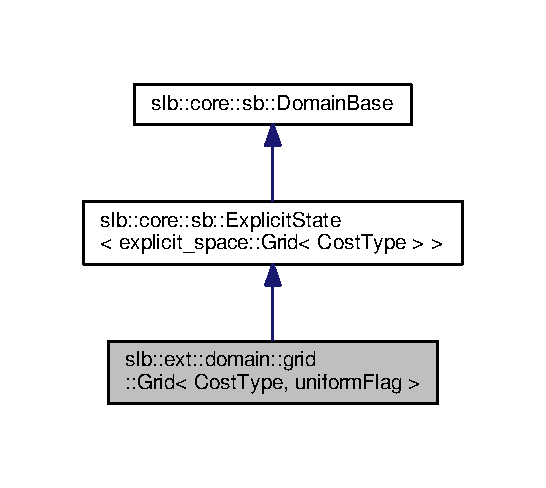
\includegraphics[width=262pt]{structslb_1_1ext_1_1domain_1_1grid_1_1Grid__inherit__graph}
\end{center}
\end{figure}


Collaboration diagram for slb\+:\+:ext\+:\+:domain\+:\+:grid\+:\+:Grid$<$ Cost\+Type, uniform\+Flag $>$\+:\nopagebreak
\begin{figure}[H]
\begin{center}
\leavevmode
\includegraphics[width=350pt]{structslb_1_1ext_1_1domain_1_1grid_1_1Grid__coll__graph}
\end{center}
\end{figure}
\subsubsection*{Public Types}
\begin{DoxyCompactItemize}
\item 
using \hyperlink{structslb_1_1ext_1_1domain_1_1grid_1_1Grid_a88a3253b98b7f322a609351a3b467c1c}{Base} = \hyperlink{structslb_1_1core_1_1sb_1_1ExplicitState}{Explicit\+State}$<$ \hyperlink{structslb_1_1ext_1_1explicit__space_1_1Grid}{explicit\+\_\+space\+::\+Grid}$<$ \hyperlink{structslb_1_1core_1_1sb_1_1ExplicitState_ae36e0763ad9b7ee7407aa316d4c64f14}{Cost\+Type} $>$$>$\hypertarget{structslb_1_1ext_1_1domain_1_1grid_1_1Grid_a88a3253b98b7f322a609351a3b467c1c}{}\label{structslb_1_1ext_1_1domain_1_1grid_1_1Grid_a88a3253b98b7f322a609351a3b467c1c}

\begin{DoxyCompactList}\small\item\em The base class. \end{DoxyCompactList}\item 
using \hyperlink{structslb_1_1ext_1_1domain_1_1grid_1_1Grid_a03885678f7bc1ee3a2e408439e1ff3a5}{My\+Type} = \hyperlink{structslb_1_1ext_1_1domain_1_1grid_1_1Grid}{Grid}$<$ \hyperlink{structslb_1_1core_1_1sb_1_1ExplicitState_ae36e0763ad9b7ee7407aa316d4c64f14}{Cost\+Type}, uniform\+Flag $>$
\begin{DoxyCompactList}\small\item\em $<$ Inherit constructors \end{DoxyCompactList}\item 
using \hyperlink{structslb_1_1ext_1_1domain_1_1grid_1_1Grid_a4e0d521edf3400571fd0b09e4de106a9}{S\+Neighbor} = \hyperlink{structslb_1_1core_1_1sb_1_1StateNeighbor}{State\+Neighbor}$<$ \hyperlink{structslb_1_1ext_1_1domain_1_1grid_1_1Grid_a03885678f7bc1ee3a2e408439e1ff3a5}{My\+Type}, uniform\+Flag $>$\hypertarget{structslb_1_1ext_1_1domain_1_1grid_1_1Grid_a4e0d521edf3400571fd0b09e4de106a9}{}\label{structslb_1_1ext_1_1domain_1_1grid_1_1Grid_a4e0d521edf3400571fd0b09e4de106a9}

\begin{DoxyCompactList}\small\item\em The type for representing a single neighbor state. Every domain must provide this name. \end{DoxyCompactList}\end{DoxyCompactItemize}
\subsubsection*{Public Member Functions}
\begin{DoxyCompactItemize}
\item 
std\+::vector$<$ \hyperlink{structslb_1_1ext_1_1domain_1_1grid_1_1Grid_a4e0d521edf3400571fd0b09e4de106a9}{S\+Neighbor} $>$ \hyperlink{structslb_1_1ext_1_1domain_1_1grid_1_1Grid_a623d27e882e88ec3cb6fce26424a79a3}{state\+Successors} () const 
\begin{DoxyCompactList}\small\item\em Computes the neighbors of the state. \end{DoxyCompactList}\item 
void \hyperlink{structslb_1_1ext_1_1domain_1_1grid_1_1Grid_aa419a05314d9f6a6376a503a51fcfcb9}{visual\+Location} (double \&x, double \&y) const 
\begin{DoxyCompactList}\small\item\em Fills out the coordinates for the vertex representing the state. \end{DoxyCompactList}\end{DoxyCompactItemize}
\subsubsection*{Static Public Member Functions}
\begin{DoxyCompactItemize}
\item 
static \hyperlink{structslb_1_1ext_1_1domain_1_1grid_1_1Grid}{Grid} \hyperlink{structslb_1_1ext_1_1domain_1_1grid_1_1Grid_acfd3ef8b9c3c5591b6937da526ac7613}{random} ()
\begin{DoxyCompactList}\small\item\em Returns a random state. \end{DoxyCompactList}\end{DoxyCompactItemize}


\subsubsection{Detailed Description}
\subsubsection*{template$<$typename Cost\+Type, bool uniform\+Flag$>$\\*
struct slb\+::ext\+::domain\+::grid\+::\+Grid$<$ Cost\+Type, uniform\+Flag $>$}

Explicit state specific to the \hyperlink{structslb_1_1ext_1_1domain_1_1grid_1_1Grid}{Grid} Map domain. 


\begin{DoxyTemplParams}{Template Parameters}
{\em Cost\+Type} & The type representing the cost of actions in the domain. The default value is {\ttfamily S\+L\+B\+\_\+\+C\+O\+S\+T\+\_\+\+T\+Y\+PE}. \\
\hline
{\em uniform\+Flag} & Determines whether the domain is a uniform cost one or not. The default value is {\ttfamily S\+L\+B\+\_\+\+U\+N\+I\+F\+O\+R\+M\+\_\+\+D\+O\+M\+A\+IN}. \\
\hline
\end{DoxyTemplParams}


Definition at line 22 of file grid.\+h.



\subsubsection{Member Typedef Documentation}
\index{slb\+::ext\+::domain\+::grid\+::\+Grid@{slb\+::ext\+::domain\+::grid\+::\+Grid}!My\+Type@{My\+Type}}
\index{My\+Type@{My\+Type}!slb\+::ext\+::domain\+::grid\+::\+Grid@{slb\+::ext\+::domain\+::grid\+::\+Grid}}
\paragraph[{\texorpdfstring{My\+Type}{MyType}}]{\setlength{\rightskip}{0pt plus 5cm}template$<$typename Cost\+Type , bool uniform\+Flag$>$ using {\bf slb\+::ext\+::domain\+::grid\+::\+Grid}$<$ {\bf Cost\+Type}, uniform\+Flag $>$\+::{\bf My\+Type} =  {\bf Grid}$<${\bf Cost\+Type}, uniform\+Flag$>$}\hypertarget{structslb_1_1ext_1_1domain_1_1grid_1_1Grid_a03885678f7bc1ee3a2e408439e1ff3a5}{}\label{structslb_1_1ext_1_1domain_1_1grid_1_1Grid_a03885678f7bc1ee3a2e408439e1ff3a5}


$<$ Inherit constructors 

This state type. 

Definition at line 28 of file grid.\+h.



\subsubsection{Member Function Documentation}
\index{slb\+::ext\+::domain\+::grid\+::\+Grid@{slb\+::ext\+::domain\+::grid\+::\+Grid}!random@{random}}
\index{random@{random}!slb\+::ext\+::domain\+::grid\+::\+Grid@{slb\+::ext\+::domain\+::grid\+::\+Grid}}
\paragraph[{\texorpdfstring{random()}{random()}}]{\setlength{\rightskip}{0pt plus 5cm}template$<$typename Cost\+Type , bool uniform\+Flag$>$ static {\bf Grid} {\bf slb\+::ext\+::domain\+::grid\+::\+Grid}$<$ {\bf Cost\+Type}, uniform\+Flag $>$\+::random (
\begin{DoxyParamCaption}
{}
\end{DoxyParamCaption}
)\hspace{0.3cm}{\ttfamily [inline]}, {\ttfamily [static]}}\hypertarget{structslb_1_1ext_1_1domain_1_1grid_1_1Grid_acfd3ef8b9c3c5591b6937da526ac7613}{}\label{structslb_1_1ext_1_1domain_1_1grid_1_1Grid_acfd3ef8b9c3c5591b6937da526ac7613}


Returns a random state. 

\begin{DoxyReturn}{Returns}
A random state. 
\end{DoxyReturn}


Definition at line 49 of file grid.\+h.

\index{slb\+::ext\+::domain\+::grid\+::\+Grid@{slb\+::ext\+::domain\+::grid\+::\+Grid}!state\+Successors@{state\+Successors}}
\index{state\+Successors@{state\+Successors}!slb\+::ext\+::domain\+::grid\+::\+Grid@{slb\+::ext\+::domain\+::grid\+::\+Grid}}
\paragraph[{\texorpdfstring{state\+Successors() const }{stateSuccessors() const }}]{\setlength{\rightskip}{0pt plus 5cm}template$<$typename Cost\+Type , bool uniform\+Flag$>$ std\+::vector$<${\bf S\+Neighbor}$>$ {\bf slb\+::ext\+::domain\+::grid\+::\+Grid}$<$ {\bf Cost\+Type}, uniform\+Flag $>$\+::state\+Successors (
\begin{DoxyParamCaption}
{}
\end{DoxyParamCaption}
) const\hspace{0.3cm}{\ttfamily [inline]}}\hypertarget{structslb_1_1ext_1_1domain_1_1grid_1_1Grid_a623d27e882e88ec3cb6fce26424a79a3}{}\label{structslb_1_1ext_1_1domain_1_1grid_1_1Grid_a623d27e882e88ec3cb6fce26424a79a3}


Computes the neighbors of the state. 

\begin{DoxyReturn}{Returns}
Vector of neighbors of the state. 
\end{DoxyReturn}


Definition at line 36 of file grid.\+h.

\index{slb\+::ext\+::domain\+::grid\+::\+Grid@{slb\+::ext\+::domain\+::grid\+::\+Grid}!visual\+Location@{visual\+Location}}
\index{visual\+Location@{visual\+Location}!slb\+::ext\+::domain\+::grid\+::\+Grid@{slb\+::ext\+::domain\+::grid\+::\+Grid}}
\paragraph[{\texorpdfstring{visual\+Location(double \&x, double \&y) const }{visualLocation(double &x, double &y) const }}]{\setlength{\rightskip}{0pt plus 5cm}template$<$typename Cost\+Type , bool uniform\+Flag$>$ void {\bf slb\+::ext\+::domain\+::grid\+::\+Grid}$<$ {\bf Cost\+Type}, uniform\+Flag $>$\+::visual\+Location (
\begin{DoxyParamCaption}
\item[{double \&}]{x, }
\item[{double \&}]{y}
\end{DoxyParamCaption}
) const\hspace{0.3cm}{\ttfamily [inline]}}\hypertarget{structslb_1_1ext_1_1domain_1_1grid_1_1Grid_aa419a05314d9f6a6376a503a51fcfcb9}{}\label{structslb_1_1ext_1_1domain_1_1grid_1_1Grid_aa419a05314d9f6a6376a503a51fcfcb9}


Fills out the coordinates for the vertex representing the state. 


\begin{DoxyParams}{Parameters}
{\em x} & The x-\/coordinate to be filled out. \\
\hline
{\em y} & The y-\/coordinate to be filled out. \\
\hline
\end{DoxyParams}


Definition at line 43 of file grid.\+h.



The documentation for this struct was generated from the following file\+:\begin{DoxyCompactItemize}
\item 
extensions/domains/\hyperlink{domains_2grid_8h}{grid.\+h}\end{DoxyCompactItemize}

\hypertarget{structslb_1_1core_1_1ui_1_1GroupLock}{}\subsection{slb\+:\+:core\+:\+:ui\+:\+:Group\+Lock Struct Reference}
\label{structslb_1_1core_1_1ui_1_1GroupLock}\index{slb\+::core\+::ui\+::\+Group\+Lock@{slb\+::core\+::ui\+::\+Group\+Lock}}


A \hyperlink{structslb_1_1core_1_1ui_1_1GroupLock}{Group\+Lock} object is created in order that the following drawing is done in a group, possibly on top of the current drawing. ~\newline
It cares for a lot of nitty-\/gritty details without which strange things happen. ~\newline
Uses \hyperlink{structslb_1_1core_1_1ui_1_1PatternLock}{Pattern\+Lock} to implement its functionality.  




{\ttfamily \#include $<$graphics\+\_\+object.\+h$>$}



Collaboration diagram for slb\+:\+:core\+:\+:ui\+:\+:Group\+Lock\+:\nopagebreak
\begin{figure}[H]
\begin{center}
\leavevmode
\includegraphics[width=201pt]{structslb_1_1core_1_1ui_1_1GroupLock__coll__graph}
\end{center}
\end{figure}
\subsubsection*{Public Member Functions}
\begin{DoxyCompactItemize}
\item 
\hyperlink{structslb_1_1core_1_1ui_1_1GroupLock_a556cc6347987f79027a0674e636f17d0}{Group\+Lock} (bool flag, \hyperlink{structslb_1_1core_1_1ui_1_1Graphics}{Graphics} \&g, bool clear\+Flag=false)
\begin{DoxyCompactList}\small\item\em Saves the current drawing and starts a group for the drawing commands following the lock acquisition (i.\+e. creation of the \hyperlink{structslb_1_1core_1_1ui_1_1GroupLock}{Group\+Lock} object). Clears the drawing if needed. \end{DoxyCompactList}\item 
\hyperlink{structslb_1_1core_1_1ui_1_1GroupLock_a9abd52ac58f58be639caf4313b07f94e}{$\sim$\+Group\+Lock} ()\hypertarget{structslb_1_1core_1_1ui_1_1GroupLock_a9abd52ac58f58be639caf4313b07f94e}{}\label{structslb_1_1core_1_1ui_1_1GroupLock_a9abd52ac58f58be639caf4313b07f94e}

\begin{DoxyCompactList}\small\item\em Appends the group the the current drawing. \end{DoxyCompactList}\end{DoxyCompactItemize}
\subsubsection*{Private Member Functions}
\begin{DoxyCompactItemize}
\item 
void \hyperlink{structslb_1_1core_1_1ui_1_1GroupLock_a447f62e417fbad50968be9a5edcb83c2}{virtual\+Translate} ()
\begin{DoxyCompactList}\small\item\em Translate the surface, so its top-\/left corner corresponds to the top-\/left corner of the window. This enables the margins. \end{DoxyCompactList}\item 
void \hyperlink{structslb_1_1core_1_1ui_1_1GroupLock_a7a7e70c5bcafc779330c54d935b383c1}{real\+Translate} ()\hypertarget{structslb_1_1core_1_1ui_1_1GroupLock_a7a7e70c5bcafc779330c54d935b383c1}{}\label{structslb_1_1core_1_1ui_1_1GroupLock_a7a7e70c5bcafc779330c54d935b383c1}

\begin{DoxyCompactList}\small\item\em Restore the translation matrix that was modified by \hyperlink{structslb_1_1core_1_1ui_1_1GroupLock_a447f62e417fbad50968be9a5edcb83c2}{virtual\+Translate}. \end{DoxyCompactList}\end{DoxyCompactItemize}
\subsubsection*{Private Attributes}
\begin{DoxyCompactItemize}
\item 
\hyperlink{structslb_1_1core_1_1ui_1_1Graphics}{Graphics} \& \hyperlink{structslb_1_1core_1_1ui_1_1GroupLock_a597c8a52164d6928d9feaeb8c5dcc0cf}{g\+\_\+}\hypertarget{structslb_1_1core_1_1ui_1_1GroupLock_a597c8a52164d6928d9feaeb8c5dcc0cf}{}\label{structslb_1_1core_1_1ui_1_1GroupLock_a597c8a52164d6928d9feaeb8c5dcc0cf}

\begin{DoxyCompactList}\small\item\em The graphics object. \end{DoxyCompactList}\end{DoxyCompactItemize}
\begin{Indent}{\bf Translation at the time of lock acquisition.}\par
{\em Indicates whether the lock should be acquired. }\begin{DoxyCompactItemize}
\item 
double {\bfseries orig\+Delta\+X\+\_\+}\hypertarget{structslb_1_1core_1_1ui_1_1GroupLock_af031134beaa5282e1ee0d6c5251268b0}{}\label{structslb_1_1core_1_1ui_1_1GroupLock_af031134beaa5282e1ee0d6c5251268b0}

\item 
double {\bfseries orig\+Delta\+Y\+\_\+}\hypertarget{structslb_1_1core_1_1ui_1_1GroupLock_ad138851240fca7a62f71ff2e9ece5611}{}\label{structslb_1_1core_1_1ui_1_1GroupLock_ad138851240fca7a62f71ff2e9ece5611}

\end{DoxyCompactItemize}
\end{Indent}


\subsubsection{Detailed Description}
A \hyperlink{structslb_1_1core_1_1ui_1_1GroupLock}{Group\+Lock} object is created in order that the following drawing is done in a group, possibly on top of the current drawing. ~\newline
It cares for a lot of nitty-\/gritty details without which strange things happen. ~\newline
Uses \hyperlink{structslb_1_1core_1_1ui_1_1PatternLock}{Pattern\+Lock} to implement its functionality. 

\begin{DoxyWarning}{Warning}
I got this right after a lot of trial and error. Do not try to modify this unless you are a graphics person who knows what he is doing. 
\end{DoxyWarning}


Definition at line 222 of file graphics\+\_\+object.\+h.



\subsubsection{Constructor \& Destructor Documentation}
\index{slb\+::core\+::ui\+::\+Group\+Lock@{slb\+::core\+::ui\+::\+Group\+Lock}!Group\+Lock@{Group\+Lock}}
\index{Group\+Lock@{Group\+Lock}!slb\+::core\+::ui\+::\+Group\+Lock@{slb\+::core\+::ui\+::\+Group\+Lock}}
\paragraph[{\texorpdfstring{Group\+Lock(bool flag, Graphics \&g, bool clear\+Flag=false)}{GroupLock(bool flag, Graphics &g, bool clearFlag=false)}}]{\setlength{\rightskip}{0pt plus 5cm}slb\+::core\+::ui\+::\+Group\+Lock\+::\+Group\+Lock (
\begin{DoxyParamCaption}
\item[{bool}]{flag, }
\item[{{\bf Graphics} \&}]{g, }
\item[{bool}]{clear\+Flag = {\ttfamily false}}
\end{DoxyParamCaption}
)\hspace{0.3cm}{\ttfamily [inline]}}\hypertarget{structslb_1_1core_1_1ui_1_1GroupLock_a556cc6347987f79027a0674e636f17d0}{}\label{structslb_1_1core_1_1ui_1_1GroupLock_a556cc6347987f79027a0674e636f17d0}


Saves the current drawing and starts a group for the drawing commands following the lock acquisition (i.\+e. creation of the \hyperlink{structslb_1_1core_1_1ui_1_1GroupLock}{Group\+Lock} object). Clears the drawing if needed. 


\begin{DoxyParams}{Parameters}
{\em flag} & If {\ttfamily false}, no lock is acquired. This enables a function where whether \hyperlink{structslb_1_1core_1_1ui_1_1GroupLock}{Group\+Lock} should be acquired or not is a parameter. \\
\hline
{\em g} & The graphics object. \\
\hline
{\em clear\+Flag} & If {\ttfamily true}, the previous drawing needs is cleared. \\
\hline
\end{DoxyParams}


Definition at line 230 of file graphics\+\_\+object.\+h.



\subsubsection{Member Function Documentation}
\index{slb\+::core\+::ui\+::\+Group\+Lock@{slb\+::core\+::ui\+::\+Group\+Lock}!virtual\+Translate@{virtual\+Translate}}
\index{virtual\+Translate@{virtual\+Translate}!slb\+::core\+::ui\+::\+Group\+Lock@{slb\+::core\+::ui\+::\+Group\+Lock}}
\paragraph[{\texorpdfstring{virtual\+Translate()}{virtualTranslate()}}]{\setlength{\rightskip}{0pt plus 5cm}void slb\+::core\+::ui\+::\+Group\+Lock\+::virtual\+Translate (
\begin{DoxyParamCaption}
{}
\end{DoxyParamCaption}
)\hspace{0.3cm}{\ttfamily [inline]}, {\ttfamily [private]}}\hypertarget{structslb_1_1core_1_1ui_1_1GroupLock_a447f62e417fbad50968be9a5edcb83c2}{}\label{structslb_1_1core_1_1ui_1_1GroupLock_a447f62e417fbad50968be9a5edcb83c2}


Translate the surface, so its top-\/left corner corresponds to the top-\/left corner of the window. This enables the margins. 

\begin{DoxySeeAlso}{See also}
\hyperlink{structslb_1_1core_1_1ui_1_1Graphics_a9fd508fc1907290c21608fdcd03918b4}{Graphics\+::margin} 
\end{DoxySeeAlso}


Definition at line 278 of file graphics\+\_\+object.\+h.



The documentation for this struct was generated from the following file\+:\begin{DoxyCompactItemize}
\item 
core/user\+\_\+interface/\hyperlink{graphics__object_8h}{graphics\+\_\+object.\+h}\end{DoxyCompactItemize}

\hypertarget{structslb_1_1ext_1_1heuristic_1_1differential_1_1H}{}\subsection{slb\+:\+:ext\+:\+:heuristic\+:\+:differential\+:\+:H$<$ State, Base\+Heuristic, Placement, Index\+With\+Inverse, Compact\+Index $>$ Struct Template Reference}
\label{structslb_1_1ext_1_1heuristic_1_1differential_1_1H}\index{slb\+::ext\+::heuristic\+::differential\+::\+H$<$ State, Base\+Heuristic, Placement, Index\+With\+Inverse, Compact\+Index $>$@{slb\+::ext\+::heuristic\+::differential\+::\+H$<$ State, Base\+Heuristic, Placement, Index\+With\+Inverse, Compact\+Index $>$}}


The differential heuristic. Specializations are for particular placement strategies.  




{\ttfamily \#include $<$differential.\+h$>$}



\subsubsection{Detailed Description}
\subsubsection*{template$<$class State = S\+L\+B\+\_\+\+S\+T\+A\+TE, class Base\+Heuristic = S\+L\+B\+\_\+\+D\+I\+F\+F\+E\+R\+E\+N\+T\+I\+A\+L\+\_\+\+B\+A\+S\+E\+\_\+\+H\+E\+U\+R\+I\+S\+T\+IC, class Placement = S\+L\+B\+\_\+\+D\+I\+F\+F\+E\+R\+E\+N\+T\+I\+A\+L\+\_\+\+P\+L\+A\+C\+E\+M\+E\+NT, class Index\+With\+Inverse = S\+L\+B\+\_\+\+D\+I\+F\+F\+E\+R\+E\+N\+T\+I\+A\+L\+\_\+\+I\+N\+D\+E\+X\+\_\+\+W\+I\+T\+H\+\_\+\+I\+N\+V\+E\+R\+SE, class Compact\+Index = S\+L\+B\+\_\+\+D\+I\+F\+F\+E\+R\+E\+N\+T\+I\+A\+L\+\_\+\+C\+O\+M\+P\+A\+C\+T\+\_\+\+I\+N\+D\+EX$>$\\*
struct slb\+::ext\+::heuristic\+::differential\+::\+H$<$ State, Base\+Heuristic, Placement, Index\+With\+Inverse, Compact\+Index $>$}

The differential heuristic. Specializations are for particular placement strategies. 


\begin{DoxyTemplParams}{Template Parameters}
{\em State} & The state type representing the search domain. \\
\hline
{\em Base\+Heuristic} & The underlying heuristic. \\
\hline
{\em Placement} & The pivot placement strategy. \\
\hline
{\em Index\+With\+Inverse} & Mapping of states to indices with an inverse function. \\
\hline
{\em Compact\+Index} & Mapping of states to indices that tries to use a small (or even sequential) range of indices. \\
\hline
\end{DoxyTemplParams}


Definition at line 122 of file differential.\+h.



The documentation for this struct was generated from the following file\+:\begin{DoxyCompactItemize}
\item 
extensions/heuristics/differential/\hyperlink{differential_8h}{differential.\+h}\end{DoxyCompactItemize}

\hypertarget{structslb_1_1ext_1_1heuristic_1_1differential_1_1H_3_01State_00_01BaseHeuristic_00_01Furthest_0071671274a92eae86902a47a514057667}{}\subsection{slb\+:\+:ext\+:\+:heuristic\+:\+:differential\+:\+:H$<$ State, Base\+Heuristic, Furthest, Index\+With\+Inverse, Compact\+Index $>$ Struct Template Reference}
\label{structslb_1_1ext_1_1heuristic_1_1differential_1_1H_3_01State_00_01BaseHeuristic_00_01Furthest_0071671274a92eae86902a47a514057667}\index{slb\+::ext\+::heuristic\+::differential\+::\+H$<$ State, Base\+Heuristic, Furthest, Index\+With\+Inverse, Compact\+Index $>$@{slb\+::ext\+::heuristic\+::differential\+::\+H$<$ State, Base\+Heuristic, Furthest, Index\+With\+Inverse, Compact\+Index $>$}}


The differential heuristic with the furthest placement strategy.  




{\ttfamily \#include $<$differential.\+h$>$}



Inheritance diagram for slb\+:\+:ext\+:\+:heuristic\+:\+:differential\+:\+:H$<$ State, Base\+Heuristic, Furthest, Index\+With\+Inverse, Compact\+Index $>$\+:\nopagebreak
\begin{figure}[H]
\begin{center}
\leavevmode
\includegraphics[width=255pt]{structslb_1_1ext_1_1heuristic_1_1differential_1_1H_3_01State_00_01BaseHeuristic_00_01Furthest_00c620e7ab6ca309a15f26cb410bb0cd3f}
\end{center}
\end{figure}


Collaboration diagram for slb\+:\+:ext\+:\+:heuristic\+:\+:differential\+:\+:H$<$ State, Base\+Heuristic, Furthest, Index\+With\+Inverse, Compact\+Index $>$\+:\nopagebreak
\begin{figure}[H]
\begin{center}
\leavevmode
\includegraphics[width=350pt]{structslb_1_1ext_1_1heuristic_1_1differential_1_1H_3_01State_00_01BaseHeuristic_00_01Furthest_00e9395ee60bcf979f0e0cccc90c5a7dfe}
\end{center}
\end{figure}
\subsubsection*{Public Types}
\begin{DoxyCompactItemize}
\item 
using \hyperlink{structslb_1_1ext_1_1heuristic_1_1differential_1_1H_3_01State_00_01BaseHeuristic_00_01Furthest_0071671274a92eae86902a47a514057667_a11a59768ca1e8307b7b69daa0b0197ed}{My\+Base} = \hyperlink{structslb_1_1ext_1_1heuristic_1_1differential_1_1HBase}{H\+Base}$<$ State, Base\+Heuristic, Compact\+Index $>$\hypertarget{structslb_1_1ext_1_1heuristic_1_1differential_1_1H_3_01State_00_01BaseHeuristic_00_01Furthest_0071671274a92eae86902a47a514057667_a11a59768ca1e8307b7b69daa0b0197ed}{}\label{structslb_1_1ext_1_1heuristic_1_1differential_1_1H_3_01State_00_01BaseHeuristic_00_01Furthest_0071671274a92eae86902a47a514057667_a11a59768ca1e8307b7b69daa0b0197ed}

\begin{DoxyCompactList}\small\item\em The direct base type. \end{DoxyCompactList}\end{DoxyCompactItemize}
\subsubsection*{Public Member Functions}
\begin{DoxyCompactItemize}
\item 
\hyperlink{structslb_1_1ext_1_1heuristic_1_1differential_1_1H_3_01State_00_01BaseHeuristic_00_01Furthest_0071671274a92eae86902a47a514057667_a719b3510be70cd0c8d6d1f562973db12}{H} (const State \&goal)
\begin{DoxyCompactList}\small\item\em The constructor. \end{DoxyCompactList}\item 
virtual void \hyperlink{structslb_1_1ext_1_1heuristic_1_1differential_1_1H_3_01State_00_01BaseHeuristic_00_01Furthest_0071671274a92eae86902a47a514057667_af63742c56f7bc521f323db6881477713}{my\+Make\+Pivots} ()\hypertarget{structslb_1_1ext_1_1heuristic_1_1differential_1_1H_3_01State_00_01BaseHeuristic_00_01Furthest_0071671274a92eae86902a47a514057667_af63742c56f7bc521f323db6881477713}{}\label{structslb_1_1ext_1_1heuristic_1_1differential_1_1H_3_01State_00_01BaseHeuristic_00_01Furthest_0071671274a92eae86902a47a514057667_af63742c56f7bc521f323db6881477713}

\begin{DoxyCompactList}\small\item\em Computes pivot placement. \end{DoxyCompactList}\end{DoxyCompactItemize}
\subsubsection*{Private Member Functions}
\begin{DoxyCompactItemize}
\item 
State \hyperlink{structslb_1_1ext_1_1heuristic_1_1differential_1_1H_3_01State_00_01BaseHeuristic_00_01Furthest_0071671274a92eae86902a47a514057667_a6ad762f8a4b0180df31211adb80747c6}{first\+Pivot} ()
\begin{DoxyCompactList}\small\item\em Computes the location of the first pivot. \end{DoxyCompactList}\end{DoxyCompactItemize}
\subsubsection*{Additional Inherited Members}


\subsubsection{Detailed Description}
\subsubsection*{template$<$class State, class Base\+Heuristic, class Index\+With\+Inverse, class Compact\+Index$>$\\*
struct slb\+::ext\+::heuristic\+::differential\+::\+H$<$ State, Base\+Heuristic, Furthest, Index\+With\+Inverse, Compact\+Index $>$}

The differential heuristic with the furthest placement strategy. 


\begin{DoxyTemplParams}{Template Parameters}
{\em State} & The state type representing the search domain. \\
\hline
{\em Base\+Heuristic} & The underlying heuristic. \\
\hline
{\em Placement} & The pivot placement strategy. \\
\hline
{\em Index\+With\+Inverse} & Mapping of states to indices with an inverse function. \\
\hline
{\em Compact\+Index} & Mapping of states to indices that tries to use a small (or even sequential) range of indices. \\
\hline
\end{DoxyTemplParams}


Definition at line 134 of file differential.\+h.



\subsubsection{Constructor \& Destructor Documentation}
\index{slb\+::ext\+::heuristic\+::differential\+::\+H$<$ State, Base\+Heuristic, Furthest, Index\+With\+Inverse, Compact\+Index $>$@{slb\+::ext\+::heuristic\+::differential\+::\+H$<$ State, Base\+Heuristic, Furthest, Index\+With\+Inverse, Compact\+Index $>$}!H@{H}}
\index{H@{H}!slb\+::ext\+::heuristic\+::differential\+::\+H$<$ State, Base\+Heuristic, Furthest, Index\+With\+Inverse, Compact\+Index $>$@{slb\+::ext\+::heuristic\+::differential\+::\+H$<$ State, Base\+Heuristic, Furthest, Index\+With\+Inverse, Compact\+Index $>$}}
\paragraph[{\texorpdfstring{H(const State \&goal)}{H(const State &goal)}}]{\setlength{\rightskip}{0pt plus 5cm}template$<$class State , class Base\+Heuristic , class Index\+With\+Inverse , class Compact\+Index $>$ {\bf slb\+::ext\+::heuristic\+::differential\+::H}$<$ State, Base\+Heuristic, {\bf Furthest}, Index\+With\+Inverse, Compact\+Index $>$\+::{\bf H} (
\begin{DoxyParamCaption}
\item[{const State \&}]{goal}
\end{DoxyParamCaption}
)\hspace{0.3cm}{\ttfamily [inline]}}\hypertarget{structslb_1_1ext_1_1heuristic_1_1differential_1_1H_3_01State_00_01BaseHeuristic_00_01Furthest_0071671274a92eae86902a47a514057667_a719b3510be70cd0c8d6d1f562973db12}{}\label{structslb_1_1ext_1_1heuristic_1_1differential_1_1H_3_01State_00_01BaseHeuristic_00_01Furthest_0071671274a92eae86902a47a514057667_a719b3510be70cd0c8d6d1f562973db12}


The constructor. 


\begin{DoxyParams}{Parameters}
{\em goal} & The goal state. \\
\hline
\end{DoxyParams}


Definition at line 146 of file differential.\+h.



\subsubsection{Member Function Documentation}
\index{slb\+::ext\+::heuristic\+::differential\+::\+H$<$ State, Base\+Heuristic, Furthest, Index\+With\+Inverse, Compact\+Index $>$@{slb\+::ext\+::heuristic\+::differential\+::\+H$<$ State, Base\+Heuristic, Furthest, Index\+With\+Inverse, Compact\+Index $>$}!first\+Pivot@{first\+Pivot}}
\index{first\+Pivot@{first\+Pivot}!slb\+::ext\+::heuristic\+::differential\+::\+H$<$ State, Base\+Heuristic, Furthest, Index\+With\+Inverse, Compact\+Index $>$@{slb\+::ext\+::heuristic\+::differential\+::\+H$<$ State, Base\+Heuristic, Furthest, Index\+With\+Inverse, Compact\+Index $>$}}
\paragraph[{\texorpdfstring{first\+Pivot()}{firstPivot()}}]{\setlength{\rightskip}{0pt plus 5cm}template$<$class State , class Base\+Heuristic , class Index\+With\+Inverse , class Compact\+Index $>$ State {\bf slb\+::ext\+::heuristic\+::differential\+::H}$<$ State, Base\+Heuristic, {\bf Furthest}, Index\+With\+Inverse, Compact\+Index $>$\+::first\+Pivot (
\begin{DoxyParamCaption}
{}
\end{DoxyParamCaption}
)\hspace{0.3cm}{\ttfamily [inline]}, {\ttfamily [private]}}\hypertarget{structslb_1_1ext_1_1heuristic_1_1differential_1_1H_3_01State_00_01BaseHeuristic_00_01Furthest_0071671274a92eae86902a47a514057667_a6ad762f8a4b0180df31211adb80747c6}{}\label{structslb_1_1ext_1_1heuristic_1_1differential_1_1H_3_01State_00_01BaseHeuristic_00_01Furthest_0071671274a92eae86902a47a514057667_a6ad762f8a4b0180df31211adb80747c6}


Computes the location of the first pivot. 

\begin{DoxyReturn}{Returns}
The state, which is the first pivot. 
\end{DoxyReturn}


Definition at line 168 of file differential.\+h.



The documentation for this struct was generated from the following file\+:\begin{DoxyCompactItemize}
\item 
extensions/heuristics/differential/\hyperlink{differential_8h}{differential.\+h}\end{DoxyCompactItemize}

\hypertarget{structslb_1_1core_1_1ui_1_1has__layout}{}\subsection{slb\+:\+:core\+:\+:ui\+:\+:has\+\_\+layout$<$ State, typename $>$ Struct Template Reference}
\label{structslb_1_1core_1_1ui_1_1has__layout}\index{slb\+::core\+::ui\+::has\+\_\+layout$<$ State, typename $>$@{slb\+::core\+::ui\+::has\+\_\+layout$<$ State, typename $>$}}


Declared only if {\ttfamily State} does not have a function for computing layout.  




{\ttfamily \#include $<$drawer.\+h$>$}



Inheritance diagram for slb\+:\+:core\+:\+:ui\+:\+:has\+\_\+layout$<$ State, typename $>$\+:\nopagebreak
\begin{figure}[H]
\begin{center}
\leavevmode
\includegraphics[width=218pt]{structslb_1_1core_1_1ui_1_1has__layout__inherit__graph}
\end{center}
\end{figure}


Collaboration diagram for slb\+:\+:core\+:\+:ui\+:\+:has\+\_\+layout$<$ State, typename $>$\+:\nopagebreak
\begin{figure}[H]
\begin{center}
\leavevmode
\includegraphics[width=218pt]{structslb_1_1core_1_1ui_1_1has__layout__coll__graph}
\end{center}
\end{figure}


\subsubsection{Detailed Description}
\subsubsection*{template$<$class State, typename = void\+\_\+t$<$$>$$>$\\*
struct slb\+::core\+::ui\+::has\+\_\+layout$<$ State, typename $>$}

Declared only if {\ttfamily State} does not have a function for computing layout. 

Definition at line 22 of file drawer.\+h.



The documentation for this struct was generated from the following file\+:\begin{DoxyCompactItemize}
\item 
core/user\+\_\+interface/\hyperlink{drawer_8h}{drawer.\+h}\end{DoxyCompactItemize}

\hypertarget{structslb_1_1ext_1_1heuristic_1_1differential_1_1HBase}{}\subsection{slb\+:\+:ext\+:\+:heuristic\+:\+:differential\+:\+:H\+Base$<$ State, Base\+Heuristic, Index $>$ Struct Template Reference}
\label{structslb_1_1ext_1_1heuristic_1_1differential_1_1HBase}\index{slb\+::ext\+::heuristic\+::differential\+::\+H\+Base$<$ State, Base\+Heuristic, Index $>$@{slb\+::ext\+::heuristic\+::differential\+::\+H\+Base$<$ State, Base\+Heuristic, Index $>$}}


The differential heuristic with unspecified placement strategy.  




{\ttfamily \#include $<$differential.\+h$>$}



Collaboration diagram for slb\+:\+:ext\+:\+:heuristic\+:\+:differential\+:\+:H\+Base$<$ State, Base\+Heuristic, Index $>$\+:\nopagebreak
\begin{figure}[H]
\begin{center}
\leavevmode
\includegraphics[width=350pt]{structslb_1_1ext_1_1heuristic_1_1differential_1_1HBase__coll__graph}
\end{center}
\end{figure}
\subsubsection*{Public Types}
\begin{DoxyCompactItemize}
\item 
using \hyperlink{structslb_1_1ext_1_1heuristic_1_1differential_1_1HBase_aef5c049026cfd3aeabd2b15d97fbbd1f}{Cost\+Type} = typename State\+::\+Cost\+Type\hypertarget{structslb_1_1ext_1_1heuristic_1_1differential_1_1HBase_aef5c049026cfd3aeabd2b15d97fbbd1f}{}\label{structslb_1_1ext_1_1heuristic_1_1differential_1_1HBase_aef5c049026cfd3aeabd2b15d97fbbd1f}

\begin{DoxyCompactList}\small\item\em The action cost type. \end{DoxyCompactList}\item 
using \hyperlink{structslb_1_1ext_1_1heuristic_1_1differential_1_1HBase_a616a127e34765bea6c069fc3faa4aafb}{Distances} = \hyperlink{structslb_1_1ext_1_1heuristic_1_1differential_1_1DistancesToPivots}{Distances\+To\+Pivots}$<$ State, Index $>$\hypertarget{structslb_1_1ext_1_1heuristic_1_1differential_1_1HBase_a616a127e34765bea6c069fc3faa4aafb}{}\label{structslb_1_1ext_1_1heuristic_1_1differential_1_1HBase_a616a127e34765bea6c069fc3faa4aafb}

\begin{DoxyCompactList}\small\item\em The type for storing distances to pivots. \end{DoxyCompactList}\end{DoxyCompactItemize}
\subsubsection*{Public Member Functions}
\begin{DoxyCompactItemize}
\item 
{\footnotesize template$<$C\+M\+D\+\_\+\+T\+P\+A\+R\+AM $>$ }\\\hyperlink{structslb_1_1ext_1_1heuristic_1_1differential_1_1HBase_ad75b1c656e17ff1446ce5356930ebef8}{H\+Base} (const State \&goal)
\begin{DoxyCompactList}\small\item\em The constructor. It is a template to handle the --n\+Pivots command line option and not create a problem for configurations without this option. \end{DoxyCompactList}\item 
\hyperlink{structslb_1_1ext_1_1heuristic_1_1differential_1_1HBase_aef5c049026cfd3aeabd2b15d97fbbd1f}{Cost\+Type} \hyperlink{structslb_1_1ext_1_1heuristic_1_1differential_1_1HBase_ae8896ffe8943d1c6882babd7d4e724a3}{operator()} (const State \&s) const 
\begin{DoxyCompactList}\small\item\em The call operator that computes the heuristic. \end{DoxyCompactList}\end{DoxyCompactItemize}
\subsubsection*{Protected Member Functions}
\begin{DoxyCompactItemize}
\item 
virtual void \hyperlink{structslb_1_1ext_1_1heuristic_1_1differential_1_1HBase_a1a0ff1f5ff5a750f2428f5241375640f}{my\+Make\+Pivots} ()=0\hypertarget{structslb_1_1ext_1_1heuristic_1_1differential_1_1HBase_a1a0ff1f5ff5a750f2428f5241375640f}{}\label{structslb_1_1ext_1_1heuristic_1_1differential_1_1HBase_a1a0ff1f5ff5a750f2428f5241375640f}

\begin{DoxyCompactList}\small\item\em Abstract virtual function for computing pivot placement. To be overrided by heuristics with a particular placement strategy. \end{DoxyCompactList}\item 
void \hyperlink{structslb_1_1ext_1_1heuristic_1_1differential_1_1HBase_aa56f8b55c82c5b2dc2e2f5c7a4a4d203}{make\+Pivots} ()\hypertarget{structslb_1_1ext_1_1heuristic_1_1differential_1_1HBase_aa56f8b55c82c5b2dc2e2f5c7a4a4d203}{}\label{structslb_1_1ext_1_1heuristic_1_1differential_1_1HBase_aa56f8b55c82c5b2dc2e2f5c7a4a4d203}

\begin{DoxyCompactList}\small\item\em Computes pivot placement. Defers the actual work to my\+Make\+Pivots. \end{DoxyCompactList}\item 
void \hyperlink{structslb_1_1ext_1_1heuristic_1_1differential_1_1HBase_aa2ad978bc22d55014671017da92e57f7}{fill\+Goal\+To\+Pivots} ()\hypertarget{structslb_1_1ext_1_1heuristic_1_1differential_1_1HBase_aa2ad978bc22d55014671017da92e57f7}{}\label{structslb_1_1ext_1_1heuristic_1_1differential_1_1HBase_aa2ad978bc22d55014671017da92e57f7}

\begin{DoxyCompactList}\small\item\em Fills goal-\/to-\/pivot distances. \end{DoxyCompactList}\end{DoxyCompactItemize}
\subsubsection*{Protected Attributes}
\begin{DoxyCompactItemize}
\item 
int \hyperlink{structslb_1_1ext_1_1heuristic_1_1differential_1_1HBase_af16f4d8f32e1dfe0b316ee8ec4648fc7}{n\+Pivots\+\_\+}\hypertarget{structslb_1_1ext_1_1heuristic_1_1differential_1_1HBase_af16f4d8f32e1dfe0b316ee8ec4648fc7}{}\label{structslb_1_1ext_1_1heuristic_1_1differential_1_1HBase_af16f4d8f32e1dfe0b316ee8ec4648fc7}

\begin{DoxyCompactList}\small\item\em Number of pivots. \end{DoxyCompactList}\item 
const State \& \hyperlink{structslb_1_1ext_1_1heuristic_1_1differential_1_1HBase_a45ab1399d03b8710ea0739f31169ec59}{goal\+\_\+}\hypertarget{structslb_1_1ext_1_1heuristic_1_1differential_1_1HBase_a45ab1399d03b8710ea0739f31169ec59}{}\label{structslb_1_1ext_1_1heuristic_1_1differential_1_1HBase_a45ab1399d03b8710ea0739f31169ec59}

\begin{DoxyCompactList}\small\item\em The goal state. \end{DoxyCompactList}\item 
std\+::vector$<$ \hyperlink{structslb_1_1ext_1_1heuristic_1_1differential_1_1HBase_aef5c049026cfd3aeabd2b15d97fbbd1f}{Cost\+Type} $>$ \hyperlink{structslb_1_1ext_1_1heuristic_1_1differential_1_1HBase_a341a171bb89d85cf0e552a0d5f603ca0}{goal\+To\+Pivots\+\_\+}\hypertarget{structslb_1_1ext_1_1heuristic_1_1differential_1_1HBase_a341a171bb89d85cf0e552a0d5f603ca0}{}\label{structslb_1_1ext_1_1heuristic_1_1differential_1_1HBase_a341a171bb89d85cf0e552a0d5f603ca0}

\begin{DoxyCompactList}\small\item\em Goal-\/to-\/pivot distances. \end{DoxyCompactList}\item 
Base\+Heuristic \hyperlink{structslb_1_1ext_1_1heuristic_1_1differential_1_1HBase_ab3d68a95e76ea433f8b5e299a7a1242e}{heuristic\+\_\+}\hypertarget{structslb_1_1ext_1_1heuristic_1_1differential_1_1HBase_ab3d68a95e76ea433f8b5e299a7a1242e}{}\label{structslb_1_1ext_1_1heuristic_1_1differential_1_1HBase_ab3d68a95e76ea433f8b5e299a7a1242e}

\begin{DoxyCompactList}\small\item\em The underlying heuristic. \end{DoxyCompactList}\end{DoxyCompactItemize}
\subsubsection*{Static Protected Attributes}
\begin{DoxyCompactItemize}
\item 
static \hyperlink{structslb_1_1ext_1_1heuristic_1_1differential_1_1HBase_a616a127e34765bea6c069fc3faa4aafb}{Distances} \hyperlink{structslb_1_1ext_1_1heuristic_1_1differential_1_1HBase_a393a3a4cad2b4c0e4c16d41c97cc27c8}{distances\+\_\+}\hypertarget{structslb_1_1ext_1_1heuristic_1_1differential_1_1HBase_a393a3a4cad2b4c0e4c16d41c97cc27c8}{}\label{structslb_1_1ext_1_1heuristic_1_1differential_1_1HBase_a393a3a4cad2b4c0e4c16d41c97cc27c8}

\begin{DoxyCompactList}\small\item\em Distances to pivots. \end{DoxyCompactList}\end{DoxyCompactItemize}


\subsubsection{Detailed Description}
\subsubsection*{template$<$class State, class Base\+Heuristic, class Index = No\+Index$>$\\*
struct slb\+::ext\+::heuristic\+::differential\+::\+H\+Base$<$ State, Base\+Heuristic, Index $>$}

The differential heuristic with unspecified placement strategy. 


\begin{DoxyTemplParams}{Template Parameters}
{\em State} & The state type representing the search domain. \\
\hline
{\em Base\+Heuristic} & The underlying heuristic. \\
\hline
{\em Index} & Mapping of states to indices. \\
\hline
\end{DoxyTemplParams}


Definition at line 45 of file differential.\+h.



\subsubsection{Constructor \& Destructor Documentation}
\index{slb\+::ext\+::heuristic\+::differential\+::\+H\+Base@{slb\+::ext\+::heuristic\+::differential\+::\+H\+Base}!H\+Base@{H\+Base}}
\index{H\+Base@{H\+Base}!slb\+::ext\+::heuristic\+::differential\+::\+H\+Base@{slb\+::ext\+::heuristic\+::differential\+::\+H\+Base}}
\paragraph[{\texorpdfstring{H\+Base(const State \&goal)}{HBase(const State &goal)}}]{\setlength{\rightskip}{0pt plus 5cm}template$<$class State, class Base\+Heuristic, class Index = No\+Index$>$ template$<$C\+M\+D\+\_\+\+T\+P\+A\+R\+AM $>$ {\bf slb\+::ext\+::heuristic\+::differential\+::\+H\+Base}$<$ State, Base\+Heuristic, Index $>$\+::{\bf H\+Base} (
\begin{DoxyParamCaption}
\item[{const State \&}]{goal}
\end{DoxyParamCaption}
)\hspace{0.3cm}{\ttfamily [inline]}}\hypertarget{structslb_1_1ext_1_1heuristic_1_1differential_1_1HBase_ad75b1c656e17ff1446ce5356930ebef8}{}\label{structslb_1_1ext_1_1heuristic_1_1differential_1_1HBase_ad75b1c656e17ff1446ce5356930ebef8}


The constructor. It is a template to handle the --n\+Pivots command line option and not create a problem for configurations without this option. 


\begin{DoxyParams}{Parameters}
{\em goal} & The goal state. \\
\hline
\end{DoxyParams}


Definition at line 56 of file differential.\+h.



\subsubsection{Member Function Documentation}
\index{slb\+::ext\+::heuristic\+::differential\+::\+H\+Base@{slb\+::ext\+::heuristic\+::differential\+::\+H\+Base}!operator()@{operator()}}
\index{operator()@{operator()}!slb\+::ext\+::heuristic\+::differential\+::\+H\+Base@{slb\+::ext\+::heuristic\+::differential\+::\+H\+Base}}
\paragraph[{\texorpdfstring{operator()(const State \&s) const }{operator()(const State &s) const }}]{\setlength{\rightskip}{0pt plus 5cm}template$<$class State, class Base\+Heuristic, class Index = No\+Index$>$ {\bf Cost\+Type} {\bf slb\+::ext\+::heuristic\+::differential\+::\+H\+Base}$<$ State, Base\+Heuristic, Index $>$\+::operator() (
\begin{DoxyParamCaption}
\item[{const State \&}]{s}
\end{DoxyParamCaption}
) const\hspace{0.3cm}{\ttfamily [inline]}}\hypertarget{structslb_1_1ext_1_1heuristic_1_1differential_1_1HBase_ae8896ffe8943d1c6882babd7d4e724a3}{}\label{structslb_1_1ext_1_1heuristic_1_1differential_1_1HBase_ae8896ffe8943d1c6882babd7d4e724a3}


The call operator that computes the heuristic. 


\begin{DoxyParams}{Parameters}
{\em s} & The state for which the heuristic needs to be computed. \\
\hline
\end{DoxyParams}
\begin{DoxyReturn}{Returns}
The heuristic from {\ttfamily s}. 
\end{DoxyReturn}


Definition at line 64 of file differential.\+h.



The documentation for this struct was generated from the following file\+:\begin{DoxyCompactItemize}
\item 
extensions/heuristics/differential/\hyperlink{differential_8h}{differential.\+h}\end{DoxyCompactItemize}

\hypertarget{structslb_1_1ext_1_1event_1_1HideLast}{}\subsection{slb\+:\+:ext\+:\+:event\+:\+:Hide\+Last$<$ Node $>$ Struct Template Reference}
\label{structslb_1_1ext_1_1event_1_1HideLast}\index{slb\+::ext\+::event\+::\+Hide\+Last$<$ Node $>$@{slb\+::ext\+::event\+::\+Hide\+Last$<$ Node $>$}}


Event that cancels the visual effect of the previous event.  




{\ttfamily \#include $<$events.\+h$>$}



Inheritance diagram for slb\+:\+:ext\+:\+:event\+:\+:Hide\+Last$<$ Node $>$\+:\nopagebreak
\begin{figure}[H]
\begin{center}
\leavevmode
\includegraphics[width=211pt]{structslb_1_1ext_1_1event_1_1HideLast__inherit__graph}
\end{center}
\end{figure}


Collaboration diagram for slb\+:\+:ext\+:\+:event\+:\+:Hide\+Last$<$ Node $>$\+:\nopagebreak
\begin{figure}[H]
\begin{center}
\leavevmode
\includegraphics[width=211pt]{structslb_1_1ext_1_1event_1_1HideLast__coll__graph}
\end{center}
\end{figure}
\subsubsection*{Private Member Functions}
\begin{DoxyCompactItemize}
\item 
std\+::string \hyperlink{structslb_1_1ext_1_1event_1_1HideLast_a9fa730d4078628681e2a2aea4d07fbee}{event\+Str} () const override
\begin{DoxyCompactList}\small\item\em Returns the string describing the event. This string is displayed in the log window. \end{DoxyCompactList}\item 
Event\+Type \hyperlink{structslb_1_1ext_1_1event_1_1HideLast_ac9fee726fd7cca33eaa55c120490aa9a}{event\+Type} () const 
\begin{DoxyCompactList}\small\item\em Returns the event type (see \hyperlink{namespaceslb_1_1core_1_1ui_ae44f7078122b3f63928fd619fadd2dcd}{slb\+::core\+::ui\+::\+Event\+Type}). \end{DoxyCompactList}\end{DoxyCompactItemize}


\subsubsection{Detailed Description}
\subsubsection*{template$<$class Node = S\+L\+B\+\_\+\+N\+O\+DE$>$\\*
struct slb\+::ext\+::event\+::\+Hide\+Last$<$ Node $>$}

Event that cancels the visual effect of the previous event. 


\begin{DoxyTemplParams}{Template Parameters}
{\em Node} & The search node type. \\
\hline
\end{DoxyTemplParams}
\begin{DoxyNote}{Note}
Previous event should be for the same state. 
\end{DoxyNote}


Definition at line 15 of file events.\+h.



\subsubsection{Member Function Documentation}
\index{slb\+::ext\+::event\+::\+Hide\+Last@{slb\+::ext\+::event\+::\+Hide\+Last}!event\+Str@{event\+Str}}
\index{event\+Str@{event\+Str}!slb\+::ext\+::event\+::\+Hide\+Last@{slb\+::ext\+::event\+::\+Hide\+Last}}
\paragraph[{\texorpdfstring{event\+Str() const override}{eventStr() const override}}]{\setlength{\rightskip}{0pt plus 5cm}template$<$class Node  = S\+L\+B\+\_\+\+N\+O\+DE$>$ std\+::string {\bf slb\+::ext\+::event\+::\+Hide\+Last}$<$ Node $>$\+::event\+Str (
\begin{DoxyParamCaption}
{}
\end{DoxyParamCaption}
) const\hspace{0.3cm}{\ttfamily [inline]}, {\ttfamily [override]}, {\ttfamily [private]}}\hypertarget{structslb_1_1ext_1_1event_1_1HideLast_a9fa730d4078628681e2a2aea4d07fbee}{}\label{structslb_1_1ext_1_1event_1_1HideLast_a9fa730d4078628681e2a2aea4d07fbee}


Returns the string describing the event. This string is displayed in the log window. 

\begin{DoxyReturn}{Returns}
The string describing the event. 
\end{DoxyReturn}


Definition at line 23 of file events.\+h.

\index{slb\+::ext\+::event\+::\+Hide\+Last@{slb\+::ext\+::event\+::\+Hide\+Last}!event\+Type@{event\+Type}}
\index{event\+Type@{event\+Type}!slb\+::ext\+::event\+::\+Hide\+Last@{slb\+::ext\+::event\+::\+Hide\+Last}}
\paragraph[{\texorpdfstring{event\+Type() const }{eventType() const }}]{\setlength{\rightskip}{0pt plus 5cm}template$<$class Node  = S\+L\+B\+\_\+\+N\+O\+DE$>$ Event\+Type {\bf slb\+::ext\+::event\+::\+Hide\+Last}$<$ Node $>$\+::event\+Type (
\begin{DoxyParamCaption}
{}
\end{DoxyParamCaption}
) const\hspace{0.3cm}{\ttfamily [inline]}, {\ttfamily [private]}}\hypertarget{structslb_1_1ext_1_1event_1_1HideLast_ac9fee726fd7cca33eaa55c120490aa9a}{}\label{structslb_1_1ext_1_1event_1_1HideLast_ac9fee726fd7cca33eaa55c120490aa9a}


Returns the event type (see \hyperlink{namespaceslb_1_1core_1_1ui_ae44f7078122b3f63928fd619fadd2dcd}{slb\+::core\+::ui\+::\+Event\+Type}). 

\begin{DoxyReturn}{Returns}
The event type. 
\end{DoxyReturn}


Definition at line 27 of file events.\+h.



The documentation for this struct was generated from the following file\+:\begin{DoxyCompactItemize}
\item 
extensions/events/\hyperlink{events_8h}{events.\+h}\end{DoxyCompactItemize}

\hypertarget{structslb_1_1ext_1_1algorithm_1_1IdAstar}{}\subsection{slb\+:\+:ext\+:\+:algorithm\+:\+:Id\+Astar$<$ A\+L\+G\+\_\+\+T\+P\+A\+R\+A\+MS, Backtrack\+Lock\+\_\+, Pruning $>$ Struct Template Reference}
\label{structslb_1_1ext_1_1algorithm_1_1IdAstar}\index{slb\+::ext\+::algorithm\+::\+Id\+Astar$<$ A\+L\+G\+\_\+\+T\+P\+A\+R\+A\+M\+S, Backtrack\+Lock\+\_\+, Pruning $>$@{slb\+::ext\+::algorithm\+::\+Id\+Astar$<$ A\+L\+G\+\_\+\+T\+P\+A\+R\+A\+M\+S, Backtrack\+Lock\+\_\+, Pruning $>$}}


The {\ttfamily I\+D\+A$\ast$} search algorithm.  




{\ttfamily \#include $<$id\+\_\+astar.\+h$>$}



Inheritance diagram for slb\+:\+:ext\+:\+:algorithm\+:\+:Id\+Astar$<$ A\+L\+G\+\_\+\+T\+P\+A\+R\+A\+MS, Backtrack\+Lock\+\_\+, Pruning $>$\+:\nopagebreak
\begin{figure}[H]
\begin{center}
\leavevmode
\includegraphics[width=350pt]{structslb_1_1ext_1_1algorithm_1_1IdAstar__inherit__graph}
\end{center}
\end{figure}


Collaboration diagram for slb\+:\+:ext\+:\+:algorithm\+:\+:Id\+Astar$<$ A\+L\+G\+\_\+\+T\+P\+A\+R\+A\+MS, Backtrack\+Lock\+\_\+, Pruning $>$\+:\nopagebreak
\begin{figure}[H]
\begin{center}
\leavevmode
\includegraphics[width=350pt]{structslb_1_1ext_1_1algorithm_1_1IdAstar__coll__graph}
\end{center}
\end{figure}
\subsubsection*{Public Types}
\begin{DoxyCompactItemize}
\item 
using \hyperlink{structslb_1_1ext_1_1algorithm_1_1IdAstar_a3b1c66ba098103b55a32545be40256e8}{Direct\+Base} = \hyperlink{structslb_1_1ext_1_1algorithm_1_1Algorithm}{Algorithm}$<$ \hyperlink{structslb_1_1ext_1_1algorithm_1_1IdAstar}{Id\+Astar}$<$ \hyperlink{algorithm_8h_a425b5a86fe8dae889a8343e14267c3c0}{A\+L\+G\+\_\+\+T\+A\+R\+GS}, Backtrack\+Lock\+\_\+ $>$, \hyperlink{algorithm_8h_a425b5a86fe8dae889a8343e14267c3c0}{A\+L\+G\+\_\+\+T\+A\+R\+GS} $>$\hypertarget{structslb_1_1ext_1_1algorithm_1_1IdAstar_a3b1c66ba098103b55a32545be40256e8}{}\label{structslb_1_1ext_1_1algorithm_1_1IdAstar_a3b1c66ba098103b55a32545be40256e8}

\begin{DoxyCompactList}\small\item\em The direct base. \end{DoxyCompactList}\item 
using \hyperlink{structslb_1_1ext_1_1algorithm_1_1IdAstar_a5a4300b273ca541f97e1ae86a1d09967}{Goal\+Handler} = typename \hyperlink{structslb_1_1ext_1_1algorithm_1_1Algorithm_ae0c6a75028107e4642e43798f21f4bfc}{Direct\+Base\+::\+Goal\+Handler}\hypertarget{structslb_1_1ext_1_1algorithm_1_1IdAstar_a5a4300b273ca541f97e1ae86a1d09967}{}\label{structslb_1_1ext_1_1algorithm_1_1IdAstar_a5a4300b273ca541f97e1ae86a1d09967}

\begin{DoxyCompactList}\small\item\em The goal handler policy. \end{DoxyCompactList}\item 
using \hyperlink{structslb_1_1ext_1_1algorithm_1_1IdAstar_a8fbd0ea83656e8d8d3bd56efccd57a43}{Initial\+Heuristic} = typename \hyperlink{structslb_1_1ext_1_1algorithm_1_1Algorithm_ad1f8f28e7b07f747ef7b7b5bf0643c2d}{Direct\+Base\+::\+Initial\+Heuristic}\hypertarget{structslb_1_1ext_1_1algorithm_1_1IdAstar_a8fbd0ea83656e8d8d3bd56efccd57a43}{}\label{structslb_1_1ext_1_1algorithm_1_1IdAstar_a8fbd0ea83656e8d8d3bd56efccd57a43}

\begin{DoxyCompactList}\small\item\em The initial heuristic policy. \end{DoxyCompactList}\item 
using \hyperlink{structslb_1_1ext_1_1algorithm_1_1IdAstar_a617d9f62e80522edaf3c25d2bf1af9ec}{Generator} = typename \hyperlink{structslb_1_1ext_1_1algorithm_1_1Algorithm_afa5a78c048b4fe4f5848aeaf5c1f8d65}{Direct\+Base\+::\+Generator}\hypertarget{structslb_1_1ext_1_1algorithm_1_1IdAstar_a617d9f62e80522edaf3c25d2bf1af9ec}{}\label{structslb_1_1ext_1_1algorithm_1_1IdAstar_a617d9f62e80522edaf3c25d2bf1af9ec}

\begin{DoxyCompactList}\small\item\em The generator policy. \end{DoxyCompactList}\item 
using \hyperlink{structslb_1_1ext_1_1algorithm_1_1IdAstar_a8c382f5126c7c1038ecd676e75e174db}{Neighbor} = typename Generator\+::\+Neighbor\hypertarget{structslb_1_1ext_1_1algorithm_1_1IdAstar_a8c382f5126c7c1038ecd676e75e174db}{}\label{structslb_1_1ext_1_1algorithm_1_1IdAstar_a8c382f5126c7c1038ecd676e75e174db}

\begin{DoxyCompactList}\small\item\em Search neighbor type. \end{DoxyCompactList}\item 
using \hyperlink{structslb_1_1ext_1_1algorithm_1_1IdAstar_ad4e2a7d07a9256a0973ed8ee0b6b6136}{My\+Type} = \hyperlink{structslb_1_1ext_1_1algorithm_1_1IdAstar}{Id\+Astar}\hypertarget{structslb_1_1ext_1_1algorithm_1_1IdAstar_ad4e2a7d07a9256a0973ed8ee0b6b6136}{}\label{structslb_1_1ext_1_1algorithm_1_1IdAstar_ad4e2a7d07a9256a0973ed8ee0b6b6136}

\begin{DoxyCompactList}\small\item\em Required for \hyperlink{algorithm_8h_a64c012078deee9a30405e18ec11e6360}{A\+L\+G\+\_\+\+D\+A\+TA} symbol. \end{DoxyCompactList}\item 
using \hyperlink{structslb_1_1ext_1_1algorithm_1_1IdAstar_a0337b9a42a8431c19a948905c996ee6c}{Backtrack\+Lock} = Backtrack\+Lock\+\_\+$<$ \hyperlink{structslb_1_1ext_1_1algorithm_1_1IdAstar_ad4e2a7d07a9256a0973ed8ee0b6b6136}{My\+Type}, log\+Flag\+\_\+ $>$\hypertarget{structslb_1_1ext_1_1algorithm_1_1IdAstar_a0337b9a42a8431c19a948905c996ee6c}{}\label{structslb_1_1ext_1_1algorithm_1_1IdAstar_a0337b9a42a8431c19a948905c996ee6c}

\begin{DoxyCompactList}\small\item\em The locking policy for backtracking. \end{DoxyCompactList}\end{DoxyCompactItemize}
\subsubsection*{Public Member Functions}
\begin{DoxyCompactItemize}
\item 
\hyperlink{algorithm_8h_a64c012078deee9a30405e18ec11e6360}{A\+L\+G\+\_\+\+D\+A\+TA} \hyperlink{structslb_1_1ext_1_1algorithm_1_1IdAstar_aa5859833358b03f49daed0c79dd50d5b}{Id\+Astar} (const My\+Instance \&instance)
\begin{DoxyCompactList}\small\item\em Initializes the algorithm based on the problem instance. \end{DoxyCompactList}\item 
Return\+Type \hyperlink{structslb_1_1ext_1_1algorithm_1_1IdAstar_a78f79f726453f63d509f05781d505874}{run} ()
\begin{DoxyCompactList}\small\item\em Runs the algorithm. \end{DoxyCompactList}\item 
bool \hyperlink{structslb_1_1ext_1_1algorithm_1_1IdAstar_a6f217097ffc1358b69381ff9d7064367}{iteration} ()
\begin{DoxyCompactList}\small\item\em Performs a single iteration of I\+D\+A$\ast$. \end{DoxyCompactList}\end{DoxyCompactItemize}
\begin{Indent}{\bf Services for policies.}\par
\begin{DoxyCompactItemize}
\item 
Node $\ast$ {\bfseries cur} ()\hypertarget{structslb_1_1ext_1_1algorithm_1_1IdAstar_ae8df24ec87b195293efee6bb04547b00}{}\label{structslb_1_1ext_1_1algorithm_1_1IdAstar_ae8df24ec87b195293efee6bb04547b00}

\item 
const \hyperlink{structslb_1_1ext_1_1algorithm_1_1IdAstar_a0337b9a42a8431c19a948905c996ee6c}{Backtrack\+Lock} $\ast$const \& {\bfseries last\+Lock} () const \hypertarget{structslb_1_1ext_1_1algorithm_1_1IdAstar_acef009e88e01b2fe9ed2f29dfd22a3e5}{}\label{structslb_1_1ext_1_1algorithm_1_1IdAstar_acef009e88e01b2fe9ed2f29dfd22a3e5}

\item 
\hyperlink{structslb_1_1ext_1_1algorithm_1_1IdAstar_a0337b9a42a8431c19a948905c996ee6c}{Backtrack\+Lock} $\ast$\& {\bfseries last\+Lock} ()\hypertarget{structslb_1_1ext_1_1algorithm_1_1IdAstar_ad0a5c5cda6b63d8f740c401646eac29b}{}\label{structslb_1_1ext_1_1algorithm_1_1IdAstar_ad0a5c5cda6b63d8f740c401646eac29b}

\end{DoxyCompactItemize}
\end{Indent}
\subsubsection*{Private Member Functions}
\begin{DoxyCompactItemize}
\item 
bool \hyperlink{structslb_1_1ext_1_1algorithm_1_1IdAstar_a60399d66c51ba26775ea268ada4cc9dc}{threshold\+Cut\+\_\+} ()
\begin{DoxyCompactList}\small\item\em Checks whether the threshold is exceeded for the case of non-\/dynamic heuristic. If so, updates the next threshold. \end{DoxyCompactList}\item 
bool \hyperlink{structslb_1_1ext_1_1algorithm_1_1IdAstar_a7cd2bb006b878a3c21df363ef3634c51}{threshold\+Cut\+\_\+} (const \hyperlink{structslb_1_1ext_1_1algorithm_1_1IdAstar_a8c382f5126c7c1038ecd676e75e174db}{Neighbor} \&n, Cost\+Type \&newH)
\begin{DoxyCompactList}\small\item\em Checks whether the threshold is exceeded for the case of dynamic heuristic. If so, updates the next threshold. \end{DoxyCompactList}\end{DoxyCompactItemize}
\subsubsection*{Private Attributes}
\begin{DoxyCompactItemize}
\item 
std\+::unique\+\_\+ptr$<$ Node $>$ \hyperlink{structslb_1_1ext_1_1algorithm_1_1IdAstar_a06120ee32156967c7916e766a9eee34e}{cur\+\_\+}\hypertarget{structslb_1_1ext_1_1algorithm_1_1IdAstar_a06120ee32156967c7916e766a9eee34e}{}\label{structslb_1_1ext_1_1algorithm_1_1IdAstar_a06120ee32156967c7916e766a9eee34e}

\begin{DoxyCompactList}\small\item\em The currently selected node. \end{DoxyCompactList}\item 
\hyperlink{structslb_1_1ext_1_1algorithm_1_1IdAstar_a0337b9a42a8431c19a948905c996ee6c}{Backtrack\+Lock} $\ast$ \hyperlink{structslb_1_1ext_1_1algorithm_1_1IdAstar_a7d8ad74c2838c8364b4ef57baa85d734}{last\+Lock\+\_\+} = nullptr\hypertarget{structslb_1_1ext_1_1algorithm_1_1IdAstar_a7d8ad74c2838c8364b4ef57baa85d734}{}\label{structslb_1_1ext_1_1algorithm_1_1IdAstar_a7d8ad74c2838c8364b4ef57baa85d734}

\begin{DoxyCompactList}\small\item\em The last bt\+Lock. Set by the lock;. \end{DoxyCompactList}\item 
Pruning$<$ \hyperlink{structslb_1_1ext_1_1algorithm_1_1IdAstar_ad4e2a7d07a9256a0973ed8ee0b6b6136}{My\+Type} $>$ {\bfseries pruner\+\_\+}\hypertarget{structslb_1_1ext_1_1algorithm_1_1IdAstar_a67903f3f88335ce68e310c43b901bd20}{}\label{structslb_1_1ext_1_1algorithm_1_1IdAstar_a67903f3f88335ce68e310c43b901bd20}

\item 
Cost\+Type \hyperlink{structslb_1_1ext_1_1algorithm_1_1IdAstar_aa9220b05233265fa1fb3948c97cdd28d}{threshold\+\_\+}\hypertarget{structslb_1_1ext_1_1algorithm_1_1IdAstar_aa9220b05233265fa1fb3948c97cdd28d}{}\label{structslb_1_1ext_1_1algorithm_1_1IdAstar_aa9220b05233265fa1fb3948c97cdd28d}

\begin{DoxyCompactList}\small\item\em The current iteration\textquotesingle{}s cost threshold. \end{DoxyCompactList}\item 
Cost\+Type \hyperlink{structslb_1_1ext_1_1algorithm_1_1IdAstar_a97ed16a300231a6df5505436f47c844a}{next\+\_\+threshold\+\_\+}\hypertarget{structslb_1_1ext_1_1algorithm_1_1IdAstar_a97ed16a300231a6df5505436f47c844a}{}\label{structslb_1_1ext_1_1algorithm_1_1IdAstar_a97ed16a300231a6df5505436f47c844a}

\begin{DoxyCompactList}\small\item\em The cost threshold for the next iteration. \end{DoxyCompactList}\end{DoxyCompactItemize}
\subsubsection*{Additional Inherited Members}


\subsubsection{Detailed Description}
\subsubsection*{template$<$A\+L\+G\+\_\+\+T\+P\+A\+R\+A\+MS, template$<$ class, bool $>$ class Backtrack\+Lock\+\_\+ = S\+L\+B\+\_\+\+I\+D\+\_\+\+A\+S\+T\+A\+R\+\_\+\+B\+A\+C\+K\+T\+R\+A\+C\+K\+\_\+\+L\+O\+CK, template$<$ class $>$ class Pruning = S\+L\+B\+\_\+\+I\+D\+\_\+\+A\+S\+T\+A\+R\+\_\+\+P\+R\+U\+N\+I\+NG$>$\\*
struct slb\+::ext\+::algorithm\+::\+Id\+Astar$<$ A\+L\+G\+\_\+\+T\+P\+A\+R\+A\+M\+S, Backtrack\+Lock\+\_\+, Pruning $>$}

The {\ttfamily I\+D\+A$\ast$} search algorithm. 


\begin{DoxyTemplParams}{Template Parameters}
{\em log\+Flag} & If {\ttfamily true}, the events generated by the search algorithm are logged. Otherwise, they are not. \\
\hline
{\em Node\+\_\+} & The search node type. \\
\hline
{\em Goal\+Handler} & The policy for handling goal conditions. \\
\hline
{\em Initial\+Heuristic} & The initial heuristic used by the search algorithm. \\
\hline
{\em Backtrack\+Lock} & The locking policy for backtracking. \\
\hline
{\em Pruning} & The policy for pruning. \\
\hline
\end{DoxyTemplParams}
\begin{DoxyNote}{Note}
See the documentation for \hyperlink{algorithm_8h_a521ad67aee0e10fb76ee132a9d5c0768}{A\+L\+G\+\_\+\+T\+P\+A\+R\+A\+MS} and \hyperlink{algorithm_8h_a64c012078deee9a30405e18ec11e6360}{A\+L\+G\+\_\+\+D\+A\+TA}. 
\end{DoxyNote}


Definition at line 24 of file id\+\_\+astar.\+h.



\subsubsection{Constructor \& Destructor Documentation}
\index{slb\+::ext\+::algorithm\+::\+Id\+Astar@{slb\+::ext\+::algorithm\+::\+Id\+Astar}!Id\+Astar@{Id\+Astar}}
\index{Id\+Astar@{Id\+Astar}!slb\+::ext\+::algorithm\+::\+Id\+Astar@{slb\+::ext\+::algorithm\+::\+Id\+Astar}}
\paragraph[{\texorpdfstring{Id\+Astar(const My\+Instance \&instance)}{IdAstar(const MyInstance &instance)}}]{\setlength{\rightskip}{0pt plus 5cm}template$<$A\+L\+G\+\_\+\+T\+P\+A\+R\+A\+MS , template$<$ class, bool $>$ class Backtrack\+Lock\+\_\+ = S\+L\+B\+\_\+\+I\+D\+\_\+\+A\+S\+T\+A\+R\+\_\+\+B\+A\+C\+K\+T\+R\+A\+C\+K\+\_\+\+L\+O\+CK, template$<$ class $>$ class Pruning = S\+L\+B\+\_\+\+I\+D\+\_\+\+A\+S\+T\+A\+R\+\_\+\+P\+R\+U\+N\+I\+NG$>$ {\bf A\+L\+G\+\_\+\+D\+A\+TA} {\bf slb\+::ext\+::algorithm\+::\+Id\+Astar}$<$ {\bf A\+L\+G\+\_\+\+T\+P\+A\+R\+A\+MS}, Backtrack\+Lock\+\_\+, Pruning $>$\+::{\bf Id\+Astar} (
\begin{DoxyParamCaption}
\item[{const My\+Instance \&}]{instance}
\end{DoxyParamCaption}
)\hspace{0.3cm}{\ttfamily [inline]}}\hypertarget{structslb_1_1ext_1_1algorithm_1_1IdAstar_aa5859833358b03f49daed0c79dd50d5b}{}\label{structslb_1_1ext_1_1algorithm_1_1IdAstar_aa5859833358b03f49daed0c79dd50d5b}


Initializes the algorithm based on the problem instance. 


\begin{DoxyParams}{Parameters}
{\em instance} & The problem instance. \\
\hline
\end{DoxyParams}


Definition at line 84 of file id\+\_\+astar.\+h.



\subsubsection{Member Function Documentation}
\index{slb\+::ext\+::algorithm\+::\+Id\+Astar@{slb\+::ext\+::algorithm\+::\+Id\+Astar}!iteration@{iteration}}
\index{iteration@{iteration}!slb\+::ext\+::algorithm\+::\+Id\+Astar@{slb\+::ext\+::algorithm\+::\+Id\+Astar}}
\paragraph[{\texorpdfstring{iteration()}{iteration()}}]{\setlength{\rightskip}{0pt plus 5cm}template$<$A\+L\+G\+\_\+\+T\+P\+A\+R\+A\+MS , template$<$ class, bool $>$ class Backtrack\+Lock\+\_\+ = S\+L\+B\+\_\+\+I\+D\+\_\+\+A\+S\+T\+A\+R\+\_\+\+B\+A\+C\+K\+T\+R\+A\+C\+K\+\_\+\+L\+O\+CK, template$<$ class $>$ class Pruning = S\+L\+B\+\_\+\+I\+D\+\_\+\+A\+S\+T\+A\+R\+\_\+\+P\+R\+U\+N\+I\+NG$>$ bool {\bf slb\+::ext\+::algorithm\+::\+Id\+Astar}$<$ {\bf A\+L\+G\+\_\+\+T\+P\+A\+R\+A\+MS}, Backtrack\+Lock\+\_\+, Pruning $>$\+::iteration (
\begin{DoxyParamCaption}
{}
\end{DoxyParamCaption}
)\hspace{0.3cm}{\ttfamily [inline]}}\hypertarget{structslb_1_1ext_1_1algorithm_1_1IdAstar_a6f217097ffc1358b69381ff9d7064367}{}\label{structslb_1_1ext_1_1algorithm_1_1IdAstar_a6f217097ffc1358b69381ff9d7064367}


Performs a single iteration of I\+D\+A$\ast$. 

\begin{DoxyReturn}{Returns}
{\ttfamily true} if the solution has been found and {\ttfamily false} otherwise. 
\end{DoxyReturn}


Definition at line 115 of file id\+\_\+astar.\+h.

\index{slb\+::ext\+::algorithm\+::\+Id\+Astar@{slb\+::ext\+::algorithm\+::\+Id\+Astar}!run@{run}}
\index{run@{run}!slb\+::ext\+::algorithm\+::\+Id\+Astar@{slb\+::ext\+::algorithm\+::\+Id\+Astar}}
\paragraph[{\texorpdfstring{run()}{run()}}]{\setlength{\rightskip}{0pt plus 5cm}template$<$A\+L\+G\+\_\+\+T\+P\+A\+R\+A\+MS , template$<$ class, bool $>$ class Backtrack\+Lock\+\_\+ = S\+L\+B\+\_\+\+I\+D\+\_\+\+A\+S\+T\+A\+R\+\_\+\+B\+A\+C\+K\+T\+R\+A\+C\+K\+\_\+\+L\+O\+CK, template$<$ class $>$ class Pruning = S\+L\+B\+\_\+\+I\+D\+\_\+\+A\+S\+T\+A\+R\+\_\+\+P\+R\+U\+N\+I\+NG$>$ Return\+Type {\bf slb\+::ext\+::algorithm\+::\+Id\+Astar}$<$ {\bf A\+L\+G\+\_\+\+T\+P\+A\+R\+A\+MS}, Backtrack\+Lock\+\_\+, Pruning $>$\+::run (
\begin{DoxyParamCaption}
{}
\end{DoxyParamCaption}
)\hspace{0.3cm}{\ttfamily [inline]}}\hypertarget{structslb_1_1ext_1_1algorithm_1_1IdAstar_a78f79f726453f63d509f05781d505874}{}\label{structslb_1_1ext_1_1algorithm_1_1IdAstar_a78f79f726453f63d509f05781d505874}


Runs the algorithm. 

\begin{DoxyReturn}{Returns}
The solution cost. If there is no solution, then {\ttfamily Cost\+Type\{-\/1\}} is returned. 
\end{DoxyReturn}


Definition at line 92 of file id\+\_\+astar.\+h.

\index{slb\+::ext\+::algorithm\+::\+Id\+Astar@{slb\+::ext\+::algorithm\+::\+Id\+Astar}!threshold\+Cut\+\_\+@{threshold\+Cut\+\_\+}}
\index{threshold\+Cut\+\_\+@{threshold\+Cut\+\_\+}!slb\+::ext\+::algorithm\+::\+Id\+Astar@{slb\+::ext\+::algorithm\+::\+Id\+Astar}}
\paragraph[{\texorpdfstring{threshold\+Cut\+\_\+()}{thresholdCut_()}}]{\setlength{\rightskip}{0pt plus 5cm}template$<$A\+L\+G\+\_\+\+T\+P\+A\+R\+A\+MS , template$<$ class, bool $>$ class Backtrack\+Lock\+\_\+ = S\+L\+B\+\_\+\+I\+D\+\_\+\+A\+S\+T\+A\+R\+\_\+\+B\+A\+C\+K\+T\+R\+A\+C\+K\+\_\+\+L\+O\+CK, template$<$ class $>$ class Pruning = S\+L\+B\+\_\+\+I\+D\+\_\+\+A\+S\+T\+A\+R\+\_\+\+P\+R\+U\+N\+I\+NG$>$ bool {\bf slb\+::ext\+::algorithm\+::\+Id\+Astar}$<$ {\bf A\+L\+G\+\_\+\+T\+P\+A\+R\+A\+MS}, Backtrack\+Lock\+\_\+, Pruning $>$\+::threshold\+Cut\+\_\+ (
\begin{DoxyParamCaption}
{}
\end{DoxyParamCaption}
)\hspace{0.3cm}{\ttfamily [inline]}, {\ttfamily [private]}}\hypertarget{structslb_1_1ext_1_1algorithm_1_1IdAstar_a60399d66c51ba26775ea268ada4cc9dc}{}\label{structslb_1_1ext_1_1algorithm_1_1IdAstar_a60399d66c51ba26775ea268ada4cc9dc}


Checks whether the threshold is exceeded for the case of non-\/dynamic heuristic. If so, updates the next threshold. 

\begin{DoxyReturn}{Returns}
{\ttfamily true} if the threshold is exceeded and {\ttfamily false} otherwise. 
\end{DoxyReturn}


Definition at line 162 of file id\+\_\+astar.\+h.

\index{slb\+::ext\+::algorithm\+::\+Id\+Astar@{slb\+::ext\+::algorithm\+::\+Id\+Astar}!threshold\+Cut\+\_\+@{threshold\+Cut\+\_\+}}
\index{threshold\+Cut\+\_\+@{threshold\+Cut\+\_\+}!slb\+::ext\+::algorithm\+::\+Id\+Astar@{slb\+::ext\+::algorithm\+::\+Id\+Astar}}
\paragraph[{\texorpdfstring{threshold\+Cut\+\_\+(const Neighbor \&n, Cost\+Type \&new\+H)}{thresholdCut_(const Neighbor &n, CostType &newH)}}]{\setlength{\rightskip}{0pt plus 5cm}template$<$A\+L\+G\+\_\+\+T\+P\+A\+R\+A\+MS , template$<$ class, bool $>$ class Backtrack\+Lock\+\_\+ = S\+L\+B\+\_\+\+I\+D\+\_\+\+A\+S\+T\+A\+R\+\_\+\+B\+A\+C\+K\+T\+R\+A\+C\+K\+\_\+\+L\+O\+CK, template$<$ class $>$ class Pruning = S\+L\+B\+\_\+\+I\+D\+\_\+\+A\+S\+T\+A\+R\+\_\+\+P\+R\+U\+N\+I\+NG$>$ bool {\bf slb\+::ext\+::algorithm\+::\+Id\+Astar}$<$ {\bf A\+L\+G\+\_\+\+T\+P\+A\+R\+A\+MS}, Backtrack\+Lock\+\_\+, Pruning $>$\+::threshold\+Cut\+\_\+ (
\begin{DoxyParamCaption}
\item[{const {\bf Neighbor} \&}]{n, }
\item[{Cost\+Type \&}]{newH}
\end{DoxyParamCaption}
)\hspace{0.3cm}{\ttfamily [inline]}, {\ttfamily [private]}}\hypertarget{structslb_1_1ext_1_1algorithm_1_1IdAstar_a7cd2bb006b878a3c21df363ef3634c51}{}\label{structslb_1_1ext_1_1algorithm_1_1IdAstar_a7cd2bb006b878a3c21df363ef3634c51}


Checks whether the threshold is exceeded for the case of dynamic heuristic. If so, updates the next threshold. 


\begin{DoxyParams}{Parameters}
{\em n} & The current neighbor. \\
\hline
{\em newH} & The heuristic value corresponding to {\ttfamily n}. \\
\hline
\end{DoxyParams}
\begin{DoxyReturn}{Returns}
{\ttfamily true} if the threshold is exceeded and {\ttfamily false} otherwise. 
\end{DoxyReturn}


Definition at line 175 of file id\+\_\+astar.\+h.



The documentation for this struct was generated from the following file\+:\begin{DoxyCompactItemize}
\item 
extensions/algorithms/\hyperlink{id__astar_8h}{id\+\_\+astar.\+h}\end{DoxyCompactItemize}

\hypertarget{structslb_1_1ext_1_1domain_1_1incWorst_1_1IncWorst}{}\subsection{slb\+:\+:ext\+:\+:domain\+:\+:inc\+Worst\+:\+:Inc\+Worst Struct Reference}
\label{structslb_1_1ext_1_1domain_1_1incWorst_1_1IncWorst}\index{slb\+::ext\+::domain\+::inc\+Worst\+::\+Inc\+Worst@{slb\+::ext\+::domain\+::inc\+Worst\+::\+Inc\+Worst}}


The worst case example for an inconsistent heuristics.  




{\ttfamily \#include $<$inc\+\_\+worst.\+h$>$}



Inheritance diagram for slb\+:\+:ext\+:\+:domain\+:\+:inc\+Worst\+:\+:Inc\+Worst\+:\nopagebreak
\begin{figure}[H]
\begin{center}
\leavevmode
\includegraphics[width=213pt]{structslb_1_1ext_1_1domain_1_1incWorst_1_1IncWorst__inherit__graph}
\end{center}
\end{figure}


Collaboration diagram for slb\+:\+:ext\+:\+:domain\+:\+:inc\+Worst\+:\+:Inc\+Worst\+:\nopagebreak
\begin{figure}[H]
\begin{center}
\leavevmode
\includegraphics[width=213pt]{structslb_1_1ext_1_1domain_1_1incWorst_1_1IncWorst__coll__graph}
\end{center}
\end{figure}
\subsubsection*{Public Types}
\begin{DoxyCompactItemize}
\item 
using \hyperlink{structslb_1_1ext_1_1domain_1_1incWorst_1_1IncWorst_a3536d51d82cab776b7f95ad90847f46c}{Cost\+Type} = int\hypertarget{structslb_1_1ext_1_1domain_1_1incWorst_1_1IncWorst_a3536d51d82cab776b7f95ad90847f46c}{}\label{structslb_1_1ext_1_1domain_1_1incWorst_1_1IncWorst_a3536d51d82cab776b7f95ad90847f46c}

\begin{DoxyCompactList}\small\item\em The type representing the cost of actions in the domain. Every domain must provide this name. \end{DoxyCompactList}\item 
using \hyperlink{structslb_1_1ext_1_1domain_1_1incWorst_1_1IncWorst_a87bebe080571b8b793d9747bc36df3b3}{S\+Neighbor} = \hyperlink{structslb_1_1core_1_1sb_1_1StateNeighbor}{State\+Neighbor}$<$ \hyperlink{structslb_1_1ext_1_1domain_1_1incWorst_1_1IncWorst}{Inc\+Worst}, false $>$\hypertarget{structslb_1_1ext_1_1domain_1_1incWorst_1_1IncWorst_a87bebe080571b8b793d9747bc36df3b3}{}\label{structslb_1_1ext_1_1domain_1_1incWorst_1_1IncWorst_a87bebe080571b8b793d9747bc36df3b3}

\begin{DoxyCompactList}\small\item\em The type for representing a single neighbor state. Every domain must provide this name. \end{DoxyCompactList}\item 
using \hyperlink{structslb_1_1ext_1_1domain_1_1incWorst_1_1IncWorst_a1285933acd81f565206f99debac7f211}{Row} = enum\{top, bottom\}\hypertarget{structslb_1_1ext_1_1domain_1_1incWorst_1_1IncWorst_a1285933acd81f565206f99debac7f211}{}\label{structslb_1_1ext_1_1domain_1_1incWorst_1_1IncWorst_a1285933acd81f565206f99debac7f211}

\begin{DoxyCompactList}\small\item\em The type for row identification. \end{DoxyCompactList}\end{DoxyCompactItemize}
\subsubsection*{Public Member Functions}
\begin{DoxyCompactItemize}
\item 
{\footnotesize template$<$C\+M\+D\+\_\+\+T\+P\+A\+R\+AM $>$ }\\\hyperlink{structslb_1_1ext_1_1domain_1_1incWorst_1_1IncWorst_ad70a5e0d2f6274f47bd9dcc8b705a9e4}{Inc\+Worst} ()
\begin{DoxyCompactList}\small\item\em Initializes the start state. \end{DoxyCompactList}\item 
\hyperlink{structslb_1_1ext_1_1domain_1_1incWorst_1_1IncWorst_a42b5b018d022ba03769c872019f6964a}{Inc\+Worst} (int k, \hyperlink{structslb_1_1ext_1_1domain_1_1incWorst_1_1IncWorst_a1285933acd81f565206f99debac7f211}{Row} row, int n)
\begin{DoxyCompactList}\small\item\em Initializes with the given number of stages, row and the stage number. \end{DoxyCompactList}\item 
{\footnotesize template$<$C\+M\+D\+\_\+\+T\+P\+A\+R\+AM $>$ }\\\hyperlink{structslb_1_1ext_1_1domain_1_1incWorst_1_1IncWorst_aac05d62d720d36ed69157c5b7eb9edc1}{Inc\+Worst} (const std\+::string \&s)
\begin{DoxyCompactList}\small\item\em Initializes the state from a string, e.\+g. \char`\"{}\mbox{[}4, top, 2\mbox{]}\char`\"{}. \end{DoxyCompactList}\item 
\hyperlink{structslb_1_1ext_1_1domain_1_1incWorst_1_1IncWorst_a23afe56ec9c3e037c0192eb15beba263}{Inc\+Worst} (const \hyperlink{structslb_1_1ext_1_1domain_1_1incWorst_1_1IncWorst}{Inc\+Worst} \&)=default\hypertarget{structslb_1_1ext_1_1domain_1_1incWorst_1_1IncWorst_a23afe56ec9c3e037c0192eb15beba263}{}\label{structslb_1_1ext_1_1domain_1_1incWorst_1_1IncWorst_a23afe56ec9c3e037c0192eb15beba263}

\begin{DoxyCompactList}\small\item\em The default copy constructor. \end{DoxyCompactList}\item 
\hyperlink{structslb_1_1ext_1_1domain_1_1incWorst_1_1IncWorst}{Inc\+Worst} \& \hyperlink{structslb_1_1ext_1_1domain_1_1incWorst_1_1IncWorst_a28d6fefe7286d5465c6ddba1efd78451}{operator=} (const \hyperlink{structslb_1_1ext_1_1domain_1_1incWorst_1_1IncWorst}{Inc\+Worst} \&)=default
\begin{DoxyCompactList}\small\item\em The default assignment operator. \end{DoxyCompactList}\item 
std\+::vector$<$ \hyperlink{structslb_1_1ext_1_1domain_1_1incWorst_1_1IncWorst_a87bebe080571b8b793d9747bc36df3b3}{S\+Neighbor} $>$ \hyperlink{structslb_1_1ext_1_1domain_1_1incWorst_1_1IncWorst_a7bab1f2886296d75e0f4ee6b7f011cec}{state\+Successors} () const 
\begin{DoxyCompactList}\small\item\em Computes the neighbors of the state. \end{DoxyCompactList}\item 
std\+::size\+\_\+t \hyperlink{structslb_1_1ext_1_1domain_1_1incWorst_1_1IncWorst_a3aad9c235eff83efe279352aa3e861be}{hash} () const 
\begin{DoxyCompactList}\small\item\em Computes the hash-\/code of the state. \end{DoxyCompactList}\item 
{\footnotesize template$<$class Stream $>$ }\\Stream \& \hyperlink{structslb_1_1ext_1_1domain_1_1incWorst_1_1IncWorst_a40e408e18a47c4a31fa902121833fe06}{dump} (Stream \&o) const 
\begin{DoxyCompactList}\small\item\em Dumps the state to the given stream. \end{DoxyCompactList}\item 
std\+::string \hyperlink{structslb_1_1ext_1_1domain_1_1incWorst_1_1IncWorst_a7bb95f5b25f09bbd0b539f46c57a651c}{visual\+Label} () const 
\begin{DoxyCompactList}\small\item\em Returns the textual label for the vertex representing the state. \end{DoxyCompactList}\item 
std\+::string \hyperlink{structslb_1_1ext_1_1domain_1_1incWorst_1_1IncWorst_af62425a98b05688bd47731862fa57a7e}{visual\+Label} (const \hyperlink{structslb_1_1ext_1_1domain_1_1incWorst_1_1IncWorst}{Inc\+Worst} \&to) const 
\begin{DoxyCompactList}\small\item\em Returns the textual label for the edge to the given state. \end{DoxyCompactList}\item 
void \hyperlink{structslb_1_1ext_1_1domain_1_1incWorst_1_1IncWorst_ad4656b5c5db486f4d8a884c765d02e9f}{visual\+Location} (double \&x, double \&y) const 
\begin{DoxyCompactList}\small\item\em Fills out the coordinates for the vertex representing the state. \end{DoxyCompactList}\item 
bool \hyperlink{structslb_1_1ext_1_1domain_1_1incWorst_1_1IncWorst_abd60ffe4de89a9d6a9d94ae6db2901d2}{operator==} (const \hyperlink{structslb_1_1ext_1_1domain_1_1incWorst_1_1IncWorst}{Inc\+Worst} \&rhs) const 
\begin{DoxyCompactList}\small\item\em The equality operator. \end{DoxyCompactList}\end{DoxyCompactItemize}
\subsubsection*{Static Public Member Functions}
\begin{DoxyCompactItemize}
\item 
{\footnotesize template$<$C\+M\+D\+\_\+\+T\+P\+A\+R\+AM $>$ }\\static \hyperlink{structslb_1_1ext_1_1domain_1_1incWorst_1_1IncWorst}{Inc\+Worst} \hyperlink{structslb_1_1ext_1_1domain_1_1incWorst_1_1IncWorst_a0292e3369f3fa58821169813803a4b7b}{random} ()
\begin{DoxyCompactList}\small\item\em Returns a random state. \end{DoxyCompactList}\end{DoxyCompactItemize}
\subsubsection*{Private Member Functions}
\begin{DoxyCompactItemize}
\item 
bool \hyperlink{structslb_1_1ext_1_1domain_1_1incWorst_1_1IncWorst_ae809fc22c6f531af5aaa86cb314060c3}{legal} (int k, int row, int n)
\begin{DoxyCompactList}\small\item\em Checks whether the state is legal. \end{DoxyCompactList}\item 
bool \hyperlink{structslb_1_1ext_1_1domain_1_1incWorst_1_1IncWorst_ae1c7ad1756a64508e06c88d1eccb48ba}{legal} (const \hyperlink{structslb_1_1ext_1_1domain_1_1incWorst_1_1IncWorst}{Inc\+Worst} \&s)
\begin{DoxyCompactList}\small\item\em Checks whether the state is legal. \end{DoxyCompactList}\item 
int \hyperlink{structslb_1_1ext_1_1domain_1_1incWorst_1_1IncWorst_ab6270d474278f724d189de85687eae59}{cost} (const \hyperlink{structslb_1_1ext_1_1domain_1_1incWorst_1_1IncWorst}{Inc\+Worst} \&from, const \hyperlink{structslb_1_1ext_1_1domain_1_1incWorst_1_1IncWorst}{Inc\+Worst} \&to) const 
\begin{DoxyCompactList}\small\item\em Returns the cost of the given move. \end{DoxyCompactList}\end{DoxyCompactItemize}
\subsubsection*{Private Attributes}
\begin{DoxyCompactItemize}
\item 
int \hyperlink{structslb_1_1ext_1_1domain_1_1incWorst_1_1IncWorst_ad4f7cd430b8a2b1499af656784cfecfe}{k\+\_\+}\hypertarget{structslb_1_1ext_1_1domain_1_1incWorst_1_1IncWorst_ad4f7cd430b8a2b1499af656784cfecfe}{}\label{structslb_1_1ext_1_1domain_1_1incWorst_1_1IncWorst_ad4f7cd430b8a2b1499af656784cfecfe}

\begin{DoxyCompactList}\small\item\em The number of stages -\/ 1. \end{DoxyCompactList}\item 
\hyperlink{structslb_1_1ext_1_1domain_1_1incWorst_1_1IncWorst_a1285933acd81f565206f99debac7f211}{Row} \hyperlink{structslb_1_1ext_1_1domain_1_1incWorst_1_1IncWorst_a5c3bda46840a401a81472446e16b44ad}{row\+\_\+}\hypertarget{structslb_1_1ext_1_1domain_1_1incWorst_1_1IncWorst_a5c3bda46840a401a81472446e16b44ad}{}\label{structslb_1_1ext_1_1domain_1_1incWorst_1_1IncWorst_a5c3bda46840a401a81472446e16b44ad}

\begin{DoxyCompactList}\small\item\em Top or bottom row. \end{DoxyCompactList}\item 
int \hyperlink{structslb_1_1ext_1_1domain_1_1incWorst_1_1IncWorst_aa98abaa062cf78e82ac96c7333b28d77}{n\+\_\+}\hypertarget{structslb_1_1ext_1_1domain_1_1incWorst_1_1IncWorst_aa98abaa062cf78e82ac96c7333b28d77}{}\label{structslb_1_1ext_1_1domain_1_1incWorst_1_1IncWorst_aa98abaa062cf78e82ac96c7333b28d77}

\begin{DoxyCompactList}\small\item\em The stage. Stages are numbered from right to left\+: k, 0, 1, ..., k-\/1. The goal is at stage k in the top row (in contrast to the book, where the goal is in the bottom row). The start is at stage k-\/1 in the bottom row. A node in the top row has the same number as the corresponding node diagonally to the left in the bottom row. \end{DoxyCompactList}\end{DoxyCompactItemize}


\subsubsection{Detailed Description}
The worst case example for an inconsistent heuristics. 

Definition at line 37 of file inc\+\_\+worst.\+h.



\subsubsection{Constructor \& Destructor Documentation}
\index{slb\+::ext\+::domain\+::inc\+Worst\+::\+Inc\+Worst@{slb\+::ext\+::domain\+::inc\+Worst\+::\+Inc\+Worst}!Inc\+Worst@{Inc\+Worst}}
\index{Inc\+Worst@{Inc\+Worst}!slb\+::ext\+::domain\+::inc\+Worst\+::\+Inc\+Worst@{slb\+::ext\+::domain\+::inc\+Worst\+::\+Inc\+Worst}}
\paragraph[{\texorpdfstring{Inc\+Worst()}{IncWorst()}}]{\setlength{\rightskip}{0pt plus 5cm}template$<$C\+M\+D\+\_\+\+T\+P\+A\+R\+AM $>$ slb\+::ext\+::domain\+::inc\+Worst\+::\+Inc\+Worst\+::\+Inc\+Worst (
\begin{DoxyParamCaption}
{}
\end{DoxyParamCaption}
)\hspace{0.3cm}{\ttfamily [inline]}}\hypertarget{structslb_1_1ext_1_1domain_1_1incWorst_1_1IncWorst_ad70a5e0d2f6274f47bd9dcc8b705a9e4}{}\label{structslb_1_1ext_1_1domain_1_1incWorst_1_1IncWorst_ad70a5e0d2f6274f47bd9dcc8b705a9e4}


Initializes the start state. 

\begin{DoxyNote}{Note}
The function is a template to avoid instantiation when the domain is not used. Such an instantiation would result in trying to use non-\/existing command line arguments. 
\end{DoxyNote}


Definition at line 53 of file inc\+\_\+worst.\+h.

\index{slb\+::ext\+::domain\+::inc\+Worst\+::\+Inc\+Worst@{slb\+::ext\+::domain\+::inc\+Worst\+::\+Inc\+Worst}!Inc\+Worst@{Inc\+Worst}}
\index{Inc\+Worst@{Inc\+Worst}!slb\+::ext\+::domain\+::inc\+Worst\+::\+Inc\+Worst@{slb\+::ext\+::domain\+::inc\+Worst\+::\+Inc\+Worst}}
\paragraph[{\texorpdfstring{Inc\+Worst(int k, Row row, int n)}{IncWorst(int k, Row row, int n)}}]{\setlength{\rightskip}{0pt plus 5cm}slb\+::ext\+::domain\+::inc\+Worst\+::\+Inc\+Worst\+::\+Inc\+Worst (
\begin{DoxyParamCaption}
\item[{int}]{k, }
\item[{{\bf Row}}]{row, }
\item[{int}]{n}
\end{DoxyParamCaption}
)\hspace{0.3cm}{\ttfamily [inline]}}\hypertarget{structslb_1_1ext_1_1domain_1_1incWorst_1_1IncWorst_a42b5b018d022ba03769c872019f6964a}{}\label{structslb_1_1ext_1_1domain_1_1incWorst_1_1IncWorst_a42b5b018d022ba03769c872019f6964a}


Initializes with the given number of stages, row and the stage number. 


\begin{DoxyParams}{Parameters}
{\em k} & The number of stages. \\
\hline
{\em row} & The row. \\
\hline
{\em n} & The stage. \\
\hline
\end{DoxyParams}


Definition at line 61 of file inc\+\_\+worst.\+h.

\index{slb\+::ext\+::domain\+::inc\+Worst\+::\+Inc\+Worst@{slb\+::ext\+::domain\+::inc\+Worst\+::\+Inc\+Worst}!Inc\+Worst@{Inc\+Worst}}
\index{Inc\+Worst@{Inc\+Worst}!slb\+::ext\+::domain\+::inc\+Worst\+::\+Inc\+Worst@{slb\+::ext\+::domain\+::inc\+Worst\+::\+Inc\+Worst}}
\paragraph[{\texorpdfstring{Inc\+Worst(const std\+::string \&s)}{IncWorst(const std::string &s)}}]{\setlength{\rightskip}{0pt plus 5cm}template$<$C\+M\+D\+\_\+\+T\+P\+A\+R\+AM $>$ slb\+::ext\+::domain\+::inc\+Worst\+::\+Inc\+Worst\+::\+Inc\+Worst (
\begin{DoxyParamCaption}
\item[{const std\+::string \&}]{s}
\end{DoxyParamCaption}
)\hspace{0.3cm}{\ttfamily [inline]}}\hypertarget{structslb_1_1ext_1_1domain_1_1incWorst_1_1IncWorst_aac05d62d720d36ed69157c5b7eb9edc1}{}\label{structslb_1_1ext_1_1domain_1_1incWorst_1_1IncWorst_aac05d62d720d36ed69157c5b7eb9edc1}


Initializes the state from a string, e.\+g. \char`\"{}\mbox{[}4, top, 2\mbox{]}\char`\"{}. 

\begin{DoxyNote}{Note}
The function is a template to avoid instantiation when the domain is not used. Such an instantiation would result in trying to use non-\/existing command line arguments. 
\end{DoxyNote}

\begin{DoxyParams}{Parameters}
{\em s} & The string. \\
\hline
\end{DoxyParams}


Definition at line 71 of file inc\+\_\+worst.\+h.



\subsubsection{Member Function Documentation}
\index{slb\+::ext\+::domain\+::inc\+Worst\+::\+Inc\+Worst@{slb\+::ext\+::domain\+::inc\+Worst\+::\+Inc\+Worst}!cost@{cost}}
\index{cost@{cost}!slb\+::ext\+::domain\+::inc\+Worst\+::\+Inc\+Worst@{slb\+::ext\+::domain\+::inc\+Worst\+::\+Inc\+Worst}}
\paragraph[{\texorpdfstring{cost(const Inc\+Worst \&from, const Inc\+Worst \&to) const }{cost(const IncWorst &from, const IncWorst &to) const }}]{\setlength{\rightskip}{0pt plus 5cm}int slb\+::ext\+::domain\+::inc\+Worst\+::\+Inc\+Worst\+::cost (
\begin{DoxyParamCaption}
\item[{const {\bf Inc\+Worst} \&}]{from, }
\item[{const {\bf Inc\+Worst} \&}]{to}
\end{DoxyParamCaption}
) const\hspace{0.3cm}{\ttfamily [inline]}, {\ttfamily [private]}}\hypertarget{structslb_1_1ext_1_1domain_1_1incWorst_1_1IncWorst_ab6270d474278f724d189de85687eae59}{}\label{structslb_1_1ext_1_1domain_1_1incWorst_1_1IncWorst_ab6270d474278f724d189de85687eae59}


Returns the cost of the given move. 


\begin{DoxyParams}{Parameters}
{\em from} & Source state. \\
\hline
{\em to} & Target state. \\
\hline
\end{DoxyParams}
\begin{DoxyReturn}{Returns}
The cost from {\ttfamily from} to {\ttfamily to}. 
\end{DoxyReturn}


Definition at line 200 of file inc\+\_\+worst.\+h.

\index{slb\+::ext\+::domain\+::inc\+Worst\+::\+Inc\+Worst@{slb\+::ext\+::domain\+::inc\+Worst\+::\+Inc\+Worst}!dump@{dump}}
\index{dump@{dump}!slb\+::ext\+::domain\+::inc\+Worst\+::\+Inc\+Worst@{slb\+::ext\+::domain\+::inc\+Worst\+::\+Inc\+Worst}}
\paragraph[{\texorpdfstring{dump(\+Stream \&o) const }{dump(Stream &o) const }}]{\setlength{\rightskip}{0pt plus 5cm}template$<$class Stream $>$ Stream\& slb\+::ext\+::domain\+::inc\+Worst\+::\+Inc\+Worst\+::dump (
\begin{DoxyParamCaption}
\item[{Stream \&}]{o}
\end{DoxyParamCaption}
) const\hspace{0.3cm}{\ttfamily [inline]}}\hypertarget{structslb_1_1ext_1_1domain_1_1incWorst_1_1IncWorst_a40e408e18a47c4a31fa902121833fe06}{}\label{structslb_1_1ext_1_1domain_1_1incWorst_1_1IncWorst_a40e408e18a47c4a31fa902121833fe06}


Dumps the state to the given stream. 


\begin{DoxyTemplParams}{Template Parameters}
{\em The} & stream type. \\
\hline
\end{DoxyTemplParams}

\begin{DoxyParams}{Parameters}
{\em o} & The stream. \\
\hline
\end{DoxyParams}
\begin{DoxyReturn}{Returns}
The modified stream. 
\end{DoxyReturn}


Definition at line 114 of file inc\+\_\+worst.\+h.

\index{slb\+::ext\+::domain\+::inc\+Worst\+::\+Inc\+Worst@{slb\+::ext\+::domain\+::inc\+Worst\+::\+Inc\+Worst}!hash@{hash}}
\index{hash@{hash}!slb\+::ext\+::domain\+::inc\+Worst\+::\+Inc\+Worst@{slb\+::ext\+::domain\+::inc\+Worst\+::\+Inc\+Worst}}
\paragraph[{\texorpdfstring{hash() const }{hash() const }}]{\setlength{\rightskip}{0pt plus 5cm}std\+::size\+\_\+t slb\+::ext\+::domain\+::inc\+Worst\+::\+Inc\+Worst\+::hash (
\begin{DoxyParamCaption}
{}
\end{DoxyParamCaption}
) const\hspace{0.3cm}{\ttfamily [inline]}}\hypertarget{structslb_1_1ext_1_1domain_1_1incWorst_1_1IncWorst_a3aad9c235eff83efe279352aa3e861be}{}\label{structslb_1_1ext_1_1domain_1_1incWorst_1_1IncWorst_a3aad9c235eff83efe279352aa3e861be}


Computes the hash-\/code of the state. 

\begin{DoxyReturn}{Returns}
The hash-\/code of the state. 
\end{DoxyReturn}


Definition at line 104 of file inc\+\_\+worst.\+h.

\index{slb\+::ext\+::domain\+::inc\+Worst\+::\+Inc\+Worst@{slb\+::ext\+::domain\+::inc\+Worst\+::\+Inc\+Worst}!legal@{legal}}
\index{legal@{legal}!slb\+::ext\+::domain\+::inc\+Worst\+::\+Inc\+Worst@{slb\+::ext\+::domain\+::inc\+Worst\+::\+Inc\+Worst}}
\paragraph[{\texorpdfstring{legal(int k, int row, int n)}{legal(int k, int row, int n)}}]{\setlength{\rightskip}{0pt plus 5cm}bool slb\+::ext\+::domain\+::inc\+Worst\+::\+Inc\+Worst\+::legal (
\begin{DoxyParamCaption}
\item[{int}]{k, }
\item[{int}]{row, }
\item[{int}]{n}
\end{DoxyParamCaption}
)\hspace{0.3cm}{\ttfamily [inline]}, {\ttfamily [private]}}\hypertarget{structslb_1_1ext_1_1domain_1_1incWorst_1_1IncWorst_ae809fc22c6f531af5aaa86cb314060c3}{}\label{structslb_1_1ext_1_1domain_1_1incWorst_1_1IncWorst_ae809fc22c6f531af5aaa86cb314060c3}


Checks whether the state is legal. 


\begin{DoxyParams}{Parameters}
{\em k} & The number of stages. \\
\hline
{\em row} & The row. \\
\hline
{\em n} & The stage. \\
\hline
\end{DoxyParams}
\begin{DoxyReturn}{Returns}
{\ttfamily true} if the state is legal and {\ttfamily false} otherwise. 
\end{DoxyReturn}


Definition at line 182 of file inc\+\_\+worst.\+h.

\index{slb\+::ext\+::domain\+::inc\+Worst\+::\+Inc\+Worst@{slb\+::ext\+::domain\+::inc\+Worst\+::\+Inc\+Worst}!legal@{legal}}
\index{legal@{legal}!slb\+::ext\+::domain\+::inc\+Worst\+::\+Inc\+Worst@{slb\+::ext\+::domain\+::inc\+Worst\+::\+Inc\+Worst}}
\paragraph[{\texorpdfstring{legal(const Inc\+Worst \&s)}{legal(const IncWorst &s)}}]{\setlength{\rightskip}{0pt plus 5cm}bool slb\+::ext\+::domain\+::inc\+Worst\+::\+Inc\+Worst\+::legal (
\begin{DoxyParamCaption}
\item[{const {\bf Inc\+Worst} \&}]{s}
\end{DoxyParamCaption}
)\hspace{0.3cm}{\ttfamily [inline]}, {\ttfamily [private]}}\hypertarget{structslb_1_1ext_1_1domain_1_1incWorst_1_1IncWorst_ae1c7ad1756a64508e06c88d1eccb48ba}{}\label{structslb_1_1ext_1_1domain_1_1incWorst_1_1IncWorst_ae1c7ad1756a64508e06c88d1eccb48ba}


Checks whether the state is legal. 


\begin{DoxyParams}{Parameters}
{\em s} & The state. \\
\hline
\end{DoxyParams}
\begin{DoxyReturn}{Returns}
{\ttfamily true} if the state is legal and {\ttfamily false} otherwise. 
\end{DoxyReturn}


Definition at line 192 of file inc\+\_\+worst.\+h.

\index{slb\+::ext\+::domain\+::inc\+Worst\+::\+Inc\+Worst@{slb\+::ext\+::domain\+::inc\+Worst\+::\+Inc\+Worst}!operator=@{operator=}}
\index{operator=@{operator=}!slb\+::ext\+::domain\+::inc\+Worst\+::\+Inc\+Worst@{slb\+::ext\+::domain\+::inc\+Worst\+::\+Inc\+Worst}}
\paragraph[{\texorpdfstring{operator=(const Inc\+Worst \&)=default}{operator=(const IncWorst &)=default}}]{\setlength{\rightskip}{0pt plus 5cm}{\bf Inc\+Worst}\& slb\+::ext\+::domain\+::inc\+Worst\+::\+Inc\+Worst\+::operator= (
\begin{DoxyParamCaption}
\item[{const {\bf Inc\+Worst} \&}]{}
\end{DoxyParamCaption}
)\hspace{0.3cm}{\ttfamily [default]}}\hypertarget{structslb_1_1ext_1_1domain_1_1incWorst_1_1IncWorst_a28d6fefe7286d5465c6ddba1efd78451}{}\label{structslb_1_1ext_1_1domain_1_1incWorst_1_1IncWorst_a28d6fefe7286d5465c6ddba1efd78451}


The default assignment operator. 

\begin{DoxyReturn}{Returns}
Reference to the assigned state. 
\end{DoxyReturn}
\index{slb\+::ext\+::domain\+::inc\+Worst\+::\+Inc\+Worst@{slb\+::ext\+::domain\+::inc\+Worst\+::\+Inc\+Worst}!operator==@{operator==}}
\index{operator==@{operator==}!slb\+::ext\+::domain\+::inc\+Worst\+::\+Inc\+Worst@{slb\+::ext\+::domain\+::inc\+Worst\+::\+Inc\+Worst}}
\paragraph[{\texorpdfstring{operator==(const Inc\+Worst \&rhs) const }{operator==(const IncWorst &rhs) const }}]{\setlength{\rightskip}{0pt plus 5cm}bool slb\+::ext\+::domain\+::inc\+Worst\+::\+Inc\+Worst\+::operator== (
\begin{DoxyParamCaption}
\item[{const {\bf Inc\+Worst} \&}]{rhs}
\end{DoxyParamCaption}
) const\hspace{0.3cm}{\ttfamily [inline]}}\hypertarget{structslb_1_1ext_1_1domain_1_1incWorst_1_1IncWorst_abd60ffe4de89a9d6a9d94ae6db2901d2}{}\label{structslb_1_1ext_1_1domain_1_1incWorst_1_1IncWorst_abd60ffe4de89a9d6a9d94ae6db2901d2}


The equality operator. 


\begin{DoxyParams}{Parameters}
{\em rhs} & The right-\/hand side of the operator. \\
\hline
\end{DoxyParams}
\begin{DoxyReturn}{Returns}
{\ttfamily true} if the two states compare equal and {\ttfamily false} otherwise. 
\end{DoxyReturn}


Definition at line 146 of file inc\+\_\+worst.\+h.

\index{slb\+::ext\+::domain\+::inc\+Worst\+::\+Inc\+Worst@{slb\+::ext\+::domain\+::inc\+Worst\+::\+Inc\+Worst}!random@{random}}
\index{random@{random}!slb\+::ext\+::domain\+::inc\+Worst\+::\+Inc\+Worst@{slb\+::ext\+::domain\+::inc\+Worst\+::\+Inc\+Worst}}
\paragraph[{\texorpdfstring{random()}{random()}}]{\setlength{\rightskip}{0pt plus 5cm}template$<$C\+M\+D\+\_\+\+T\+P\+A\+R\+AM $>$ static {\bf Inc\+Worst} slb\+::ext\+::domain\+::inc\+Worst\+::\+Inc\+Worst\+::random (
\begin{DoxyParamCaption}
{}
\end{DoxyParamCaption}
)\hspace{0.3cm}{\ttfamily [inline]}, {\ttfamily [static]}}\hypertarget{structslb_1_1ext_1_1domain_1_1incWorst_1_1IncWorst_a0292e3369f3fa58821169813803a4b7b}{}\label{structslb_1_1ext_1_1domain_1_1incWorst_1_1IncWorst_a0292e3369f3fa58821169813803a4b7b}


Returns a random state. 

\begin{DoxyReturn}{Returns}
A random state. 
\end{DoxyReturn}
\begin{DoxyNote}{Note}
The function is a template to avoid instantiation when the domain is not used. Such an instantiation would result in trying to use non-\/existing command line arguments. 
\end{DoxyNote}


Definition at line 157 of file inc\+\_\+worst.\+h.

\index{slb\+::ext\+::domain\+::inc\+Worst\+::\+Inc\+Worst@{slb\+::ext\+::domain\+::inc\+Worst\+::\+Inc\+Worst}!state\+Successors@{state\+Successors}}
\index{state\+Successors@{state\+Successors}!slb\+::ext\+::domain\+::inc\+Worst\+::\+Inc\+Worst@{slb\+::ext\+::domain\+::inc\+Worst\+::\+Inc\+Worst}}
\paragraph[{\texorpdfstring{state\+Successors() const }{stateSuccessors() const }}]{\setlength{\rightskip}{0pt plus 5cm}std\+::vector$<${\bf S\+Neighbor}$>$ slb\+::ext\+::domain\+::inc\+Worst\+::\+Inc\+Worst\+::state\+Successors (
\begin{DoxyParamCaption}
{}
\end{DoxyParamCaption}
) const\hspace{0.3cm}{\ttfamily [inline]}}\hypertarget{structslb_1_1ext_1_1domain_1_1incWorst_1_1IncWorst_a7bab1f2886296d75e0f4ee6b7f011cec}{}\label{structslb_1_1ext_1_1domain_1_1incWorst_1_1IncWorst_a7bab1f2886296d75e0f4ee6b7f011cec}


Computes the neighbors of the state. 

\begin{DoxyReturn}{Returns}
Vector of neighbors of the state. 
\end{DoxyReturn}


Definition at line 87 of file inc\+\_\+worst.\+h.

\index{slb\+::ext\+::domain\+::inc\+Worst\+::\+Inc\+Worst@{slb\+::ext\+::domain\+::inc\+Worst\+::\+Inc\+Worst}!visual\+Label@{visual\+Label}}
\index{visual\+Label@{visual\+Label}!slb\+::ext\+::domain\+::inc\+Worst\+::\+Inc\+Worst@{slb\+::ext\+::domain\+::inc\+Worst\+::\+Inc\+Worst}}
\paragraph[{\texorpdfstring{visual\+Label() const }{visualLabel() const }}]{\setlength{\rightskip}{0pt plus 5cm}std\+::string slb\+::ext\+::domain\+::inc\+Worst\+::\+Inc\+Worst\+::visual\+Label (
\begin{DoxyParamCaption}
{}
\end{DoxyParamCaption}
) const\hspace{0.3cm}{\ttfamily [inline]}}\hypertarget{structslb_1_1ext_1_1domain_1_1incWorst_1_1IncWorst_a7bb95f5b25f09bbd0b539f46c57a651c}{}\label{structslb_1_1ext_1_1domain_1_1incWorst_1_1IncWorst_a7bb95f5b25f09bbd0b539f46c57a651c}


Returns the textual label for the vertex representing the state. 

\begin{DoxyReturn}{Returns}
The textual label for the vertex representing the state. 
\end{DoxyReturn}


Definition at line 120 of file inc\+\_\+worst.\+h.

\index{slb\+::ext\+::domain\+::inc\+Worst\+::\+Inc\+Worst@{slb\+::ext\+::domain\+::inc\+Worst\+::\+Inc\+Worst}!visual\+Label@{visual\+Label}}
\index{visual\+Label@{visual\+Label}!slb\+::ext\+::domain\+::inc\+Worst\+::\+Inc\+Worst@{slb\+::ext\+::domain\+::inc\+Worst\+::\+Inc\+Worst}}
\paragraph[{\texorpdfstring{visual\+Label(const Inc\+Worst \&to) const }{visualLabel(const IncWorst &to) const }}]{\setlength{\rightskip}{0pt plus 5cm}std\+::string slb\+::ext\+::domain\+::inc\+Worst\+::\+Inc\+Worst\+::visual\+Label (
\begin{DoxyParamCaption}
\item[{const {\bf Inc\+Worst} \&}]{to}
\end{DoxyParamCaption}
) const\hspace{0.3cm}{\ttfamily [inline]}}\hypertarget{structslb_1_1ext_1_1domain_1_1incWorst_1_1IncWorst_af62425a98b05688bd47731862fa57a7e}{}\label{structslb_1_1ext_1_1domain_1_1incWorst_1_1IncWorst_af62425a98b05688bd47731862fa57a7e}


Returns the textual label for the edge to the given state. 


\begin{DoxyParams}{Parameters}
{\em to} & The target state. \\
\hline
\end{DoxyParams}
\begin{DoxyReturn}{Returns}
The textual label for the edge to {\ttfamily to}. 
\end{DoxyReturn}


Definition at line 128 of file inc\+\_\+worst.\+h.

\index{slb\+::ext\+::domain\+::inc\+Worst\+::\+Inc\+Worst@{slb\+::ext\+::domain\+::inc\+Worst\+::\+Inc\+Worst}!visual\+Location@{visual\+Location}}
\index{visual\+Location@{visual\+Location}!slb\+::ext\+::domain\+::inc\+Worst\+::\+Inc\+Worst@{slb\+::ext\+::domain\+::inc\+Worst\+::\+Inc\+Worst}}
\paragraph[{\texorpdfstring{visual\+Location(double \&x, double \&y) const }{visualLocation(double &x, double &y) const }}]{\setlength{\rightskip}{0pt plus 5cm}void slb\+::ext\+::domain\+::inc\+Worst\+::\+Inc\+Worst\+::visual\+Location (
\begin{DoxyParamCaption}
\item[{double \&}]{x, }
\item[{double \&}]{y}
\end{DoxyParamCaption}
) const\hspace{0.3cm}{\ttfamily [inline]}}\hypertarget{structslb_1_1ext_1_1domain_1_1incWorst_1_1IncWorst_ad4656b5c5db486f4d8a884c765d02e9f}{}\label{structslb_1_1ext_1_1domain_1_1incWorst_1_1IncWorst_ad4656b5c5db486f4d8a884c765d02e9f}


Fills out the coordinates for the vertex representing the state. 


\begin{DoxyParams}{Parameters}
{\em x} & The x-\/coordinate to be filled out. \\
\hline
{\em y} & The y-\/coordinate to be filled out. \\
\hline
\end{DoxyParams}


Definition at line 135 of file inc\+\_\+worst.\+h.



The documentation for this struct was generated from the following file\+:\begin{DoxyCompactItemize}
\item 
extensions/domains/\hyperlink{inc__worst_8h}{inc\+\_\+worst.\+h}\end{DoxyCompactItemize}

\hypertarget{structslb_1_1core_1_1util_1_1IndexIterator}{}\subsection{slb\+:\+:core\+:\+:util\+:\+:Index\+Iterator$<$ My\+Vector, Base $>$ Struct Template Reference}
\label{structslb_1_1core_1_1util_1_1IndexIterator}\index{slb\+::core\+::util\+::\+Index\+Iterator$<$ My\+Vector, Base $>$@{slb\+::core\+::util\+::\+Index\+Iterator$<$ My\+Vector, Base $>$}}


Vector iterator whose dereference operator returns index instead of value.  




{\ttfamily \#include $<$container.\+h$>$}



Inheritance diagram for slb\+:\+:core\+:\+:util\+:\+:Index\+Iterator$<$ My\+Vector, Base $>$\+:\nopagebreak
\begin{figure}[H]
\begin{center}
\leavevmode
\includegraphics[width=214pt]{structslb_1_1core_1_1util_1_1IndexIterator__inherit__graph}
\end{center}
\end{figure}


Collaboration diagram for slb\+:\+:core\+:\+:util\+:\+:Index\+Iterator$<$ My\+Vector, Base $>$\+:\nopagebreak
\begin{figure}[H]
\begin{center}
\leavevmode
\includegraphics[width=214pt]{structslb_1_1core_1_1util_1_1IndexIterator__coll__graph}
\end{center}
\end{figure}
\subsubsection*{Public Member Functions}
\begin{DoxyCompactItemize}
\item 
{\footnotesize template$<$class... Args$>$ }\\\hyperlink{structslb_1_1core_1_1util_1_1IndexIterator_aa22ada12fb0a5560aabe364f98e6ecbf}{Index\+Iterator} (Args \&\&...args)
\begin{DoxyCompactList}\small\item\em Constructor. \end{DoxyCompactList}\item 
\hyperlink{structslb_1_1core_1_1util_1_1IndexIterator_a51756eb68c0db6afb8271a2170ad3f17}{Index\+Iterator} (const \hyperlink{structslb_1_1core_1_1util_1_1IndexIterator}{Index\+Iterator} \&b)
\begin{DoxyCompactList}\small\item\em Copy constructor. \end{DoxyCompactList}\item 
int \hyperlink{structslb_1_1core_1_1util_1_1IndexIterator_a666a20d111b0cb76f2694332879cc963}{operator$\ast$} () const 
\begin{DoxyCompactList}\small\item\em The dereference operator. \end{DoxyCompactList}\item 
\hyperlink{structslb_1_1core_1_1util_1_1IndexIterator}{Index\+Iterator} \& \hyperlink{structslb_1_1core_1_1util_1_1IndexIterator_aeed92994cbb11d9d4e372895dd138ba2}{operator=} (const \hyperlink{structslb_1_1core_1_1util_1_1IndexIterator}{Index\+Iterator} \&rhs)
\begin{DoxyCompactList}\small\item\em The assignment operator. \end{DoxyCompactList}\end{DoxyCompactItemize}


\subsubsection{Detailed Description}
\subsubsection*{template$<$class My\+Vector, class Base$>$\\*
struct slb\+::core\+::util\+::\+Index\+Iterator$<$ My\+Vector, Base $>$}

Vector iterator whose dereference operator returns index instead of value. 


\begin{DoxyTemplParams}{Template Parameters}
{\em My\+Vector} & The underlying vector type. \\
\hline
{\em Base} & The base iterator. Can be anything, including \hyperlink{structslb_1_1core_1_1util_1_1BasicVectorSkipIterator}{Basic\+Vector\+Skip\+Iterator}. \\
\hline
\end{DoxyTemplParams}


Definition at line 226 of file container.\+h.



\subsubsection{Constructor \& Destructor Documentation}
\index{slb\+::core\+::util\+::\+Index\+Iterator@{slb\+::core\+::util\+::\+Index\+Iterator}!Index\+Iterator@{Index\+Iterator}}
\index{Index\+Iterator@{Index\+Iterator}!slb\+::core\+::util\+::\+Index\+Iterator@{slb\+::core\+::util\+::\+Index\+Iterator}}
\paragraph[{\texorpdfstring{Index\+Iterator(\+Args \&\&...\+args)}{IndexIterator(Args &&...args)}}]{\setlength{\rightskip}{0pt plus 5cm}template$<$class My\+Vector , class Base $>$ template$<$class... Args$>$ {\bf slb\+::core\+::util\+::\+Index\+Iterator}$<$ My\+Vector, Base $>$\+::{\bf Index\+Iterator} (
\begin{DoxyParamCaption}
\item[{Args \&\&...}]{args}
\end{DoxyParamCaption}
)\hspace{0.3cm}{\ttfamily [inline]}}\hypertarget{structslb_1_1core_1_1util_1_1IndexIterator_aa22ada12fb0a5560aabe364f98e6ecbf}{}\label{structslb_1_1core_1_1util_1_1IndexIterator_aa22ada12fb0a5560aabe364f98e6ecbf}


Constructor. 


\begin{DoxyTemplParams}{Template Parameters}
{\em Args} & The argument types. \\
\hline
\end{DoxyTemplParams}

\begin{DoxyParams}{Parameters}
{\em args} & The argument list. \\
\hline
\end{DoxyParams}


Definition at line 231 of file container.\+h.

\index{slb\+::core\+::util\+::\+Index\+Iterator@{slb\+::core\+::util\+::\+Index\+Iterator}!Index\+Iterator@{Index\+Iterator}}
\index{Index\+Iterator@{Index\+Iterator}!slb\+::core\+::util\+::\+Index\+Iterator@{slb\+::core\+::util\+::\+Index\+Iterator}}
\paragraph[{\texorpdfstring{Index\+Iterator(const Index\+Iterator \&b)}{IndexIterator(const IndexIterator &b)}}]{\setlength{\rightskip}{0pt plus 5cm}template$<$class My\+Vector , class Base $>$ {\bf slb\+::core\+::util\+::\+Index\+Iterator}$<$ My\+Vector, Base $>$\+::{\bf Index\+Iterator} (
\begin{DoxyParamCaption}
\item[{const {\bf Index\+Iterator}$<$ My\+Vector, Base $>$ \&}]{b}
\end{DoxyParamCaption}
)\hspace{0.3cm}{\ttfamily [inline]}}\hypertarget{structslb_1_1core_1_1util_1_1IndexIterator_a51756eb68c0db6afb8271a2170ad3f17}{}\label{structslb_1_1core_1_1util_1_1IndexIterator_a51756eb68c0db6afb8271a2170ad3f17}


Copy constructor. 


\begin{DoxyParams}{Parameters}
{\em b} & The given iterator. \\
\hline
\end{DoxyParams}


Definition at line 235 of file container.\+h.



\subsubsection{Member Function Documentation}
\index{slb\+::core\+::util\+::\+Index\+Iterator@{slb\+::core\+::util\+::\+Index\+Iterator}!operator$\ast$@{operator$\ast$}}
\index{operator$\ast$@{operator$\ast$}!slb\+::core\+::util\+::\+Index\+Iterator@{slb\+::core\+::util\+::\+Index\+Iterator}}
\paragraph[{\texorpdfstring{operator$\ast$() const }{operator*() const }}]{\setlength{\rightskip}{0pt plus 5cm}template$<$class My\+Vector , class Base $>$ int {\bf slb\+::core\+::util\+::\+Index\+Iterator}$<$ My\+Vector, Base $>$\+::operator$\ast$ (
\begin{DoxyParamCaption}
{}
\end{DoxyParamCaption}
) const\hspace{0.3cm}{\ttfamily [inline]}}\hypertarget{structslb_1_1core_1_1util_1_1IndexIterator_a666a20d111b0cb76f2694332879cc963}{}\label{structslb_1_1core_1_1util_1_1IndexIterator_a666a20d111b0cb76f2694332879cc963}


The dereference operator. 

\begin{DoxyReturn}{Returns}
The index of the element pointed to by the iterator. 
\end{DoxyReturn}


Definition at line 239 of file container.\+h.

\index{slb\+::core\+::util\+::\+Index\+Iterator@{slb\+::core\+::util\+::\+Index\+Iterator}!operator=@{operator=}}
\index{operator=@{operator=}!slb\+::core\+::util\+::\+Index\+Iterator@{slb\+::core\+::util\+::\+Index\+Iterator}}
\paragraph[{\texorpdfstring{operator=(const Index\+Iterator \&rhs)}{operator=(const IndexIterator &rhs)}}]{\setlength{\rightskip}{0pt plus 5cm}template$<$class My\+Vector , class Base $>$ {\bf Index\+Iterator}\& {\bf slb\+::core\+::util\+::\+Index\+Iterator}$<$ My\+Vector, Base $>$\+::operator= (
\begin{DoxyParamCaption}
\item[{const {\bf Index\+Iterator}$<$ My\+Vector, Base $>$ \&}]{rhs}
\end{DoxyParamCaption}
)\hspace{0.3cm}{\ttfamily [inline]}}\hypertarget{structslb_1_1core_1_1util_1_1IndexIterator_aeed92994cbb11d9d4e372895dd138ba2}{}\label{structslb_1_1core_1_1util_1_1IndexIterator_aeed92994cbb11d9d4e372895dd138ba2}


The assignment operator. 


\begin{DoxyParams}{Parameters}
{\em rhs} & The right-\/hand side iterator. \\
\hline
\end{DoxyParams}
\begin{DoxyReturn}{Returns}
Reference to the resulting iterator. 
\end{DoxyReturn}


Definition at line 246 of file container.\+h.



The documentation for this struct was generated from the following file\+:\begin{DoxyCompactItemize}
\item 
core/util/\hyperlink{container_8h}{container.\+h}\end{DoxyCompactItemize}

\hypertarget{structslb_1_1ext_1_1policy_1_1backtrackLock_1_1Inplace}{}\subsection{slb\+:\+:ext\+:\+:policy\+:\+:backtrack\+Lock\+:\+:Inplace$<$ My\+Algorithm, bool $>$ Struct Template Reference}
\label{structslb_1_1ext_1_1policy_1_1backtrackLock_1_1Inplace}\index{slb\+::ext\+::policy\+::backtrack\+Lock\+::\+Inplace$<$ My\+Algorithm, bool $>$@{slb\+::ext\+::policy\+::backtrack\+Lock\+::\+Inplace$<$ My\+Algorithm, bool $>$}}


Handles R\+A\+II for backtracking in I\+D\+A$\ast$ when the state is updated in place.  




{\ttfamily \#include $<$backtrack\+\_\+lock.\+h$>$}



Inheritance diagram for slb\+:\+:ext\+:\+:policy\+:\+:backtrack\+Lock\+:\+:Inplace$<$ My\+Algorithm, bool $>$\+:\nopagebreak
\begin{figure}[H]
\begin{center}
\leavevmode
\includegraphics[width=250pt]{structslb_1_1ext_1_1policy_1_1backtrackLock_1_1Inplace__inherit__graph}
\end{center}
\end{figure}


Collaboration diagram for slb\+:\+:ext\+:\+:policy\+:\+:backtrack\+Lock\+:\+:Inplace$<$ My\+Algorithm, bool $>$\+:\nopagebreak
\begin{figure}[H]
\begin{center}
\leavevmode
\includegraphics[width=250pt]{structslb_1_1ext_1_1policy_1_1backtrackLock_1_1Inplace__coll__graph}
\end{center}
\end{figure}
\subsubsection*{Public Types}
\begin{DoxyCompactItemize}
\item 
using \hyperlink{structslb_1_1ext_1_1policy_1_1backtrackLock_1_1Inplace_a2668b070defebca51e8b0d420a90f68b}{Base} = \hyperlink{structslb_1_1ext_1_1policy_1_1backtrackLock_1_1InplaceBase}{Inplace\+Base}$<$ My\+Algorithm $>$\hypertarget{structslb_1_1ext_1_1policy_1_1backtrackLock_1_1Inplace_a2668b070defebca51e8b0d420a90f68b}{}\label{structslb_1_1ext_1_1policy_1_1backtrackLock_1_1Inplace_a2668b070defebca51e8b0d420a90f68b}

\begin{DoxyCompactList}\small\item\em The base class. \end{DoxyCompactList}\end{DoxyCompactItemize}
\subsubsection*{Public Member Functions}
\begin{DoxyCompactItemize}
\item 
{\footnotesize template$<$class Neighbor $>$ }\\\hyperlink{structslb_1_1ext_1_1policy_1_1backtrackLock_1_1Inplace_afde8d0b3b15952436e678b8ab265cbc1}{Inplace} (My\+Algorithm \&alg, Neighbor \&n, Cost\+Type h)
\begin{DoxyCompactList}\small\item\em The constructor. \end{DoxyCompactList}\item 
\hyperlink{structslb_1_1ext_1_1policy_1_1backtrackLock_1_1Inplace_aba500581c23a004f268e95a7865b6bf5}{Inplace} (\hyperlink{structslb_1_1ext_1_1policy_1_1backtrackLock_1_1Inplace}{Inplace} \&\&)=default\hypertarget{structslb_1_1ext_1_1policy_1_1backtrackLock_1_1Inplace_aba500581c23a004f268e95a7865b6bf5}{}\label{structslb_1_1ext_1_1policy_1_1backtrackLock_1_1Inplace_aba500581c23a004f268e95a7865b6bf5}

\begin{DoxyCompactList}\small\item\em The moving constructor. \end{DoxyCompactList}\item 
\hyperlink{structslb_1_1ext_1_1policy_1_1backtrackLock_1_1Inplace_ae63582d7aed48217b32c67c8fd69a1ec}{$\sim$\+Inplace} ()\hypertarget{structslb_1_1ext_1_1policy_1_1backtrackLock_1_1Inplace_ae63582d7aed48217b32c67c8fd69a1ec}{}\label{structslb_1_1ext_1_1policy_1_1backtrackLock_1_1Inplace_ae63582d7aed48217b32c67c8fd69a1ec}

\begin{DoxyCompactList}\small\item\em The destructor. \end{DoxyCompactList}\end{DoxyCompactItemize}
\subsubsection*{Static Public Attributes}
\begin{DoxyCompactItemize}
\item 
static const bool \hyperlink{structslb_1_1ext_1_1policy_1_1backtrackLock_1_1Inplace_a5a7d3dfd27dbf3fecd5133837f2b63e3}{keeps\+Parent} = false\hypertarget{structslb_1_1ext_1_1policy_1_1backtrackLock_1_1Inplace_a5a7d3dfd27dbf3fecd5133837f2b63e3}{}\label{structslb_1_1ext_1_1policy_1_1backtrackLock_1_1Inplace_a5a7d3dfd27dbf3fecd5133837f2b63e3}

\begin{DoxyCompactList}\small\item\em Whether the parent state is to be stored. \end{DoxyCompactList}\end{DoxyCompactItemize}
\subsubsection*{Additional Inherited Members}


\subsubsection{Detailed Description}
\subsubsection*{template$<$class My\+Algorithm, bool = false$>$\\*
struct slb\+::ext\+::policy\+::backtrack\+Lock\+::\+Inplace$<$ My\+Algorithm, bool $>$}

Handles R\+A\+II for backtracking in I\+D\+A$\ast$ when the state is updated in place. 


\begin{DoxyTemplParams}{Template Parameters}
{\em My\+Algorithm} & The search algorithm. \\
\hline
\end{DoxyTemplParams}
\begin{DoxyNote}{Note}
The second template parameter is {\ttfamily true} when the log of algorithmic events is kept (which necessitates storing the parent state) and {\ttfamily false} otherwise. 
\end{DoxyNote}


Definition at line 69 of file backtrack\+\_\+lock.\+h.



\subsubsection{Constructor \& Destructor Documentation}
\index{slb\+::ext\+::policy\+::backtrack\+Lock\+::\+Inplace@{slb\+::ext\+::policy\+::backtrack\+Lock\+::\+Inplace}!Inplace@{Inplace}}
\index{Inplace@{Inplace}!slb\+::ext\+::policy\+::backtrack\+Lock\+::\+Inplace@{slb\+::ext\+::policy\+::backtrack\+Lock\+::\+Inplace}}
\paragraph[{\texorpdfstring{Inplace(\+My\+Algorithm \&alg, Neighbor \&n, Cost\+Type h)}{Inplace(MyAlgorithm &alg, Neighbor &n, CostType h)}}]{\setlength{\rightskip}{0pt plus 5cm}template$<$class My\+Algorithm , bool  = false$>$ template$<$class Neighbor $>$ {\bf slb\+::ext\+::policy\+::backtrack\+Lock\+::\+Inplace}$<$ My\+Algorithm, bool $>$\+::{\bf Inplace} (
\begin{DoxyParamCaption}
\item[{My\+Algorithm \&}]{alg, }
\item[{Neighbor \&}]{n, }
\item[{Cost\+Type}]{h}
\end{DoxyParamCaption}
)\hspace{0.3cm}{\ttfamily [inline]}}\hypertarget{structslb_1_1ext_1_1policy_1_1backtrackLock_1_1Inplace_afde8d0b3b15952436e678b8ab265cbc1}{}\label{structslb_1_1ext_1_1policy_1_1backtrackLock_1_1Inplace_afde8d0b3b15952436e678b8ab265cbc1}


The constructor. 


\begin{DoxyTemplParams}{Template Parameters}
{\em Neighbor} & The neighbor type. \\
\hline
\end{DoxyTemplParams}

\begin{DoxyParams}{Parameters}
{\em alg} & The search algorithm. \\
\hline
{\em n} & The neighbor. \\
\hline
{\em h} & The computed heuristic for {\ttfamily n}. \\
\hline
\end{DoxyParams}


Definition at line 83 of file backtrack\+\_\+lock.\+h.



The documentation for this struct was generated from the following file\+:\begin{DoxyCompactItemize}
\item 
extensions/shared\+\_\+policies/\hyperlink{backtrack__lock_8h}{backtrack\+\_\+lock.\+h}\end{DoxyCompactItemize}

\hypertarget{structslb_1_1ext_1_1policy_1_1backtrackLock_1_1Inplace_3_01MyAlgorithm_00_01true_01_4}{}\subsection{slb\+:\+:ext\+:\+:policy\+:\+:backtrack\+Lock\+:\+:Inplace$<$ My\+Algorithm, true $>$ Struct Template Reference}
\label{structslb_1_1ext_1_1policy_1_1backtrackLock_1_1Inplace_3_01MyAlgorithm_00_01true_01_4}\index{slb\+::ext\+::policy\+::backtrack\+Lock\+::\+Inplace$<$ My\+Algorithm, true $>$@{slb\+::ext\+::policy\+::backtrack\+Lock\+::\+Inplace$<$ My\+Algorithm, true $>$}}


Handles R\+A\+II for backtracking in I\+D\+A$\ast$ when the state is updated in place and log is kept, so that a copy of the parent state needs to be kept.  




{\ttfamily \#include $<$backtrack\+\_\+lock.\+h$>$}



Inheritance diagram for slb\+:\+:ext\+:\+:policy\+:\+:backtrack\+Lock\+:\+:Inplace$<$ My\+Algorithm, true $>$\+:\nopagebreak
\begin{figure}[H]
\begin{center}
\leavevmode
\includegraphics[width=250pt]{structslb_1_1ext_1_1policy_1_1backtrackLock_1_1Inplace_3_01MyAlgorithm_00_01true_01_4__inherit__graph}
\end{center}
\end{figure}


Collaboration diagram for slb\+:\+:ext\+:\+:policy\+:\+:backtrack\+Lock\+:\+:Inplace$<$ My\+Algorithm, true $>$\+:\nopagebreak
\begin{figure}[H]
\begin{center}
\leavevmode
\includegraphics[width=250pt]{structslb_1_1ext_1_1policy_1_1backtrackLock_1_1Inplace_3_01MyAlgorithm_00_01true_01_4__coll__graph}
\end{center}
\end{figure}
\subsubsection*{Public Types}
\begin{DoxyCompactItemize}
\item 
using \hyperlink{structslb_1_1ext_1_1policy_1_1backtrackLock_1_1Inplace_3_01MyAlgorithm_00_01true_01_4_aa59da222559e46238469c23706dedd3d}{Base} = \hyperlink{structslb_1_1ext_1_1policy_1_1backtrackLock_1_1InplaceBase}{Inplace\+Base}$<$ My\+Algorithm $>$\hypertarget{structslb_1_1ext_1_1policy_1_1backtrackLock_1_1Inplace_3_01MyAlgorithm_00_01true_01_4_aa59da222559e46238469c23706dedd3d}{}\label{structslb_1_1ext_1_1policy_1_1backtrackLock_1_1Inplace_3_01MyAlgorithm_00_01true_01_4_aa59da222559e46238469c23706dedd3d}

\begin{DoxyCompactList}\small\item\em The base class. \end{DoxyCompactList}\end{DoxyCompactItemize}
\subsubsection*{Public Member Functions}
\begin{DoxyCompactItemize}
\item 
{\footnotesize template$<$class Neighbor $>$ }\\\hyperlink{structslb_1_1ext_1_1policy_1_1backtrackLock_1_1Inplace_3_01MyAlgorithm_00_01true_01_4_a6f70a5ab71cccf4d4442f43fd660a68b}{Inplace} (My\+Algorithm \&alg, Neighbor \&n, Cost\+Type h)
\begin{DoxyCompactList}\small\item\em The constructor. \end{DoxyCompactList}\item 
\hyperlink{structslb_1_1ext_1_1policy_1_1backtrackLock_1_1Inplace_3_01MyAlgorithm_00_01true_01_4_acf1e0f412c740f8c5d5936361d2f0e6f}{Inplace} (\hyperlink{structslb_1_1ext_1_1policy_1_1backtrackLock_1_1Inplace}{Inplace} \&\&)=default\hypertarget{structslb_1_1ext_1_1policy_1_1backtrackLock_1_1Inplace_3_01MyAlgorithm_00_01true_01_4_acf1e0f412c740f8c5d5936361d2f0e6f}{}\label{structslb_1_1ext_1_1policy_1_1backtrackLock_1_1Inplace_3_01MyAlgorithm_00_01true_01_4_acf1e0f412c740f8c5d5936361d2f0e6f}

\begin{DoxyCompactList}\small\item\em The moving constructor. \end{DoxyCompactList}\item 
\hyperlink{structslb_1_1ext_1_1policy_1_1backtrackLock_1_1Inplace_3_01MyAlgorithm_00_01true_01_4_a0ccbddccfba4038e9b87e2712f76cda9}{$\sim$\+Inplace} ()\hypertarget{structslb_1_1ext_1_1policy_1_1backtrackLock_1_1Inplace_3_01MyAlgorithm_00_01true_01_4_a0ccbddccfba4038e9b87e2712f76cda9}{}\label{structslb_1_1ext_1_1policy_1_1backtrackLock_1_1Inplace_3_01MyAlgorithm_00_01true_01_4_a0ccbddccfba4038e9b87e2712f76cda9}

\begin{DoxyCompactList}\small\item\em The destructor. \end{DoxyCompactList}\end{DoxyCompactItemize}
\subsubsection*{Static Public Attributes}
\begin{DoxyCompactItemize}
\item 
static const bool \hyperlink{structslb_1_1ext_1_1policy_1_1backtrackLock_1_1Inplace_3_01MyAlgorithm_00_01true_01_4_a5f637322f0bd991877c9bfb9e48bccb4}{keeps\+Parent} = true\hypertarget{structslb_1_1ext_1_1policy_1_1backtrackLock_1_1Inplace_3_01MyAlgorithm_00_01true_01_4_a5f637322f0bd991877c9bfb9e48bccb4}{}\label{structslb_1_1ext_1_1policy_1_1backtrackLock_1_1Inplace_3_01MyAlgorithm_00_01true_01_4_a5f637322f0bd991877c9bfb9e48bccb4}

\begin{DoxyCompactList}\small\item\em Whether the parent state is to be stored. \end{DoxyCompactList}\end{DoxyCompactItemize}
\subsubsection*{Private Member Functions}
\begin{DoxyCompactItemize}
\item 
{\footnotesize template$<$class Neighbor $>$ }\\void \hyperlink{structslb_1_1ext_1_1policy_1_1backtrackLock_1_1Inplace_3_01MyAlgorithm_00_01true_01_4_a20f19ca5602c8c47bc4d2cc9e4e5fac1}{set} (Neighbor \&n, Cost\+Type h)
\begin{DoxyCompactList}\small\item\em Does the necessary bookkeeping for searching the given neighbor. \end{DoxyCompactList}\item 
void \hyperlink{structslb_1_1ext_1_1policy_1_1backtrackLock_1_1Inplace_3_01MyAlgorithm_00_01true_01_4_a20c434c629d4e15d7688493da6bb79ef}{unset} ()\hypertarget{structslb_1_1ext_1_1policy_1_1backtrackLock_1_1Inplace_3_01MyAlgorithm_00_01true_01_4_a20c434c629d4e15d7688493da6bb79ef}{}\label{structslb_1_1ext_1_1policy_1_1backtrackLock_1_1Inplace_3_01MyAlgorithm_00_01true_01_4_a20c434c629d4e15d7688493da6bb79ef}

\begin{DoxyCompactList}\small\item\em Does the necessary bookkeeping before backtracking to the parent. \end{DoxyCompactList}\end{DoxyCompactItemize}
\subsubsection*{Private Attributes}
\begin{DoxyCompactItemize}
\item 
std\+::unique\+\_\+ptr$<$ Node $>$ \hyperlink{structslb_1_1ext_1_1policy_1_1backtrackLock_1_1Inplace_3_01MyAlgorithm_00_01true_01_4_a3e518436193db41ea16c569828afa795}{parent\+\_\+} = nullptr\hypertarget{structslb_1_1ext_1_1policy_1_1backtrackLock_1_1Inplace_3_01MyAlgorithm_00_01true_01_4_a3e518436193db41ea16c569828afa795}{}\label{structslb_1_1ext_1_1policy_1_1backtrackLock_1_1Inplace_3_01MyAlgorithm_00_01true_01_4_a3e518436193db41ea16c569828afa795}

\begin{DoxyCompactList}\small\item\em The parent node. \end{DoxyCompactList}\end{DoxyCompactItemize}
\subsubsection*{Additional Inherited Members}


\subsubsection{Detailed Description}
\subsubsection*{template$<$class My\+Algorithm$>$\\*
struct slb\+::ext\+::policy\+::backtrack\+Lock\+::\+Inplace$<$ My\+Algorithm, true $>$}

Handles R\+A\+II for backtracking in I\+D\+A$\ast$ when the state is updated in place and log is kept, so that a copy of the parent state needs to be kept. 


\begin{DoxyTemplParams}{Template Parameters}
{\em My\+Algorithm} & The search algorithm. \\
\hline
\end{DoxyTemplParams}


Definition at line 93 of file backtrack\+\_\+lock.\+h.



\subsubsection{Constructor \& Destructor Documentation}
\index{slb\+::ext\+::policy\+::backtrack\+Lock\+::\+Inplace$<$ My\+Algorithm, true $>$@{slb\+::ext\+::policy\+::backtrack\+Lock\+::\+Inplace$<$ My\+Algorithm, true $>$}!Inplace@{Inplace}}
\index{Inplace@{Inplace}!slb\+::ext\+::policy\+::backtrack\+Lock\+::\+Inplace$<$ My\+Algorithm, true $>$@{slb\+::ext\+::policy\+::backtrack\+Lock\+::\+Inplace$<$ My\+Algorithm, true $>$}}
\paragraph[{\texorpdfstring{Inplace(\+My\+Algorithm \&alg, Neighbor \&n, Cost\+Type h)}{Inplace(MyAlgorithm &alg, Neighbor &n, CostType h)}}]{\setlength{\rightskip}{0pt plus 5cm}template$<$class My\+Algorithm $>$ template$<$class Neighbor $>$ {\bf slb\+::ext\+::policy\+::backtrack\+Lock\+::\+Inplace}$<$ My\+Algorithm, true $>$\+::{\bf Inplace} (
\begin{DoxyParamCaption}
\item[{My\+Algorithm \&}]{alg, }
\item[{Neighbor \&}]{n, }
\item[{Cost\+Type}]{h}
\end{DoxyParamCaption}
)\hspace{0.3cm}{\ttfamily [inline]}}\hypertarget{structslb_1_1ext_1_1policy_1_1backtrackLock_1_1Inplace_3_01MyAlgorithm_00_01true_01_4_a6f70a5ab71cccf4d4442f43fd660a68b}{}\label{structslb_1_1ext_1_1policy_1_1backtrackLock_1_1Inplace_3_01MyAlgorithm_00_01true_01_4_a6f70a5ab71cccf4d4442f43fd660a68b}


The constructor. 


\begin{DoxyTemplParams}{Template Parameters}
{\em Neighbor} & The neighbor type. \\
\hline
\end{DoxyTemplParams}

\begin{DoxyParams}{Parameters}
{\em alg} & The search algorithm. \\
\hline
{\em n} & The neighbor. \\
\hline
\end{DoxyParams}


Definition at line 107 of file backtrack\+\_\+lock.\+h.



\subsubsection{Member Function Documentation}
\index{slb\+::ext\+::policy\+::backtrack\+Lock\+::\+Inplace$<$ My\+Algorithm, true $>$@{slb\+::ext\+::policy\+::backtrack\+Lock\+::\+Inplace$<$ My\+Algorithm, true $>$}!set@{set}}
\index{set@{set}!slb\+::ext\+::policy\+::backtrack\+Lock\+::\+Inplace$<$ My\+Algorithm, true $>$@{slb\+::ext\+::policy\+::backtrack\+Lock\+::\+Inplace$<$ My\+Algorithm, true $>$}}
\paragraph[{\texorpdfstring{set(\+Neighbor \&n, Cost\+Type h)}{set(Neighbor &n, CostType h)}}]{\setlength{\rightskip}{0pt plus 5cm}template$<$class My\+Algorithm $>$ template$<$class Neighbor $>$ void {\bf slb\+::ext\+::policy\+::backtrack\+Lock\+::\+Inplace}$<$ My\+Algorithm, true $>$\+::set (
\begin{DoxyParamCaption}
\item[{Neighbor \&}]{n, }
\item[{Cost\+Type}]{h}
\end{DoxyParamCaption}
)\hspace{0.3cm}{\ttfamily [inline]}, {\ttfamily [private]}}\hypertarget{structslb_1_1ext_1_1policy_1_1backtrackLock_1_1Inplace_3_01MyAlgorithm_00_01true_01_4_a20f19ca5602c8c47bc4d2cc9e4e5fac1}{}\label{structslb_1_1ext_1_1policy_1_1backtrackLock_1_1Inplace_3_01MyAlgorithm_00_01true_01_4_a20f19ca5602c8c47bc4d2cc9e4e5fac1}


Does the necessary bookkeeping for searching the given neighbor. 


\begin{DoxyTemplParams}{Template Parameters}
{\em Neighbor} & The neighbor type. \\
\hline
\end{DoxyTemplParams}

\begin{DoxyParams}{Parameters}
{\em n} & The neighbor. \\
\hline
\end{DoxyParams}


Definition at line 123 of file backtrack\+\_\+lock.\+h.



The documentation for this struct was generated from the following file\+:\begin{DoxyCompactItemize}
\item 
extensions/shared\+\_\+policies/\hyperlink{backtrack__lock_8h}{backtrack\+\_\+lock.\+h}\end{DoxyCompactItemize}

\hypertarget{structslb_1_1ext_1_1policy_1_1backtrackLock_1_1InplaceBase}{}\subsection{slb\+:\+:ext\+:\+:policy\+:\+:backtrack\+Lock\+:\+:Inplace\+Base$<$ My\+Algorithm $>$ Struct Template Reference}
\label{structslb_1_1ext_1_1policy_1_1backtrackLock_1_1InplaceBase}\index{slb\+::ext\+::policy\+::backtrack\+Lock\+::\+Inplace\+Base$<$ My\+Algorithm $>$@{slb\+::ext\+::policy\+::backtrack\+Lock\+::\+Inplace\+Base$<$ My\+Algorithm $>$}}


Base for a class handling R\+A\+II for backtracking in I\+D\+A$\ast$ when the state is updated in place (i.\+e. \hyperlink{structslb_1_1core_1_1sb_1_1ActionNeighbor}{core\+::sb\+::\+Action\+Neighbor} is used).  




{\ttfamily \#include $<$backtrack\+\_\+lock.\+h$>$}



Inheritance diagram for slb\+:\+:ext\+:\+:policy\+:\+:backtrack\+Lock\+:\+:Inplace\+Base$<$ My\+Algorithm $>$\+:\nopagebreak
\begin{figure}[H]
\begin{center}
\leavevmode
\includegraphics[width=350pt]{structslb_1_1ext_1_1policy_1_1backtrackLock_1_1InplaceBase__inherit__graph}
\end{center}
\end{figure}
\subsubsection*{Public Member Functions}
\begin{DoxyCompactItemize}
\item 
{\footnotesize template$<$class Neighbor $>$ }\\\hyperlink{extensions_2shared__policies_2headers_8h_ae70a06fa4631780beea14971eb36a562}{P\+O\+L\+I\+C\+Y\+\_\+\+T\+Y\+P\+ES} \hyperlink{structslb_1_1ext_1_1policy_1_1backtrackLock_1_1InplaceBase_a2c4eebd972539d487b44ffe23ebc4aff}{Inplace\+Base} (My\+Algorithm \&alg, Node $\ast$cur, Neighbor \&)
\begin{DoxyCompactList}\small\item\em The constructor. \end{DoxyCompactList}\end{DoxyCompactItemize}
\subsubsection*{Protected Member Functions}
\begin{DoxyCompactItemize}
\item 
{\footnotesize template$<$class Neighbor $>$ }\\void \hyperlink{structslb_1_1ext_1_1policy_1_1backtrackLock_1_1InplaceBase_a9f838f14f1b87a7c96e3475e586c93d3}{set} (Neighbor \&n)
\begin{DoxyCompactList}\small\item\em Does the necessary bookkeeping for searching the given neighbor. \end{DoxyCompactList}\item 
void \hyperlink{structslb_1_1ext_1_1policy_1_1backtrackLock_1_1InplaceBase_a5ac11057420d465ee33087c504c026e0}{unset} ()\hypertarget{structslb_1_1ext_1_1policy_1_1backtrackLock_1_1InplaceBase_a5ac11057420d465ee33087c504c026e0}{}\label{structslb_1_1ext_1_1policy_1_1backtrackLock_1_1InplaceBase_a5ac11057420d465ee33087c504c026e0}

\begin{DoxyCompactList}\small\item\em Does the necessary bookkeeping before backtracking to the parent. \end{DoxyCompactList}\end{DoxyCompactItemize}
\subsubsection*{Protected Attributes}
\begin{DoxyCompactItemize}
\item 
Node $\ast$ \hyperlink{structslb_1_1ext_1_1policy_1_1backtrackLock_1_1InplaceBase_a3e9e83ff286e8f93a4ff2d52678d4d7e}{cur\+\_\+}\hypertarget{structslb_1_1ext_1_1policy_1_1backtrackLock_1_1InplaceBase_a3e9e83ff286e8f93a4ff2d52678d4d7e}{}\label{structslb_1_1ext_1_1policy_1_1backtrackLock_1_1InplaceBase_a3e9e83ff286e8f93a4ff2d52678d4d7e}

\begin{DoxyCompactList}\small\item\em The node being expanded by I\+D\+A$\ast$. \end{DoxyCompactList}\end{DoxyCompactItemize}
\subsubsection*{Private Attributes}
\begin{DoxyCompactItemize}
\item 
My\+Algorithm \& \hyperlink{structslb_1_1ext_1_1policy_1_1backtrackLock_1_1InplaceBase_a24e865cfe03cd65824667f5a6d16a3b2}{alg\+\_\+}\hypertarget{structslb_1_1ext_1_1policy_1_1backtrackLock_1_1InplaceBase_a24e865cfe03cd65824667f5a6d16a3b2}{}\label{structslb_1_1ext_1_1policy_1_1backtrackLock_1_1InplaceBase_a24e865cfe03cd65824667f5a6d16a3b2}

\begin{DoxyCompactList}\small\item\em Reference to the search algorithm. \end{DoxyCompactList}\item 
Node\+Data \hyperlink{structslb_1_1ext_1_1policy_1_1backtrackLock_1_1InplaceBase_a984702ee6a149f5dd219ee3233c4567d}{data\+\_\+}\hypertarget{structslb_1_1ext_1_1policy_1_1backtrackLock_1_1InplaceBase_a984702ee6a149f5dd219ee3233c4567d}{}\label{structslb_1_1ext_1_1policy_1_1backtrackLock_1_1InplaceBase_a984702ee6a149f5dd219ee3233c4567d}

\begin{DoxyCompactList}\small\item\em The data stored with the parent node. \end{DoxyCompactList}\item 
State\+::\+Action \hyperlink{structslb_1_1ext_1_1policy_1_1backtrackLock_1_1InplaceBase_afcc45c39856522b24e6d23e3417eb0cb}{reverse\+Action\+\_\+}\hypertarget{structslb_1_1ext_1_1policy_1_1backtrackLock_1_1InplaceBase_afcc45c39856522b24e6d23e3417eb0cb}{}\label{structslb_1_1ext_1_1policy_1_1backtrackLock_1_1InplaceBase_afcc45c39856522b24e6d23e3417eb0cb}

\begin{DoxyCompactList}\small\item\em The action that takes back to the parent. \end{DoxyCompactList}\end{DoxyCompactItemize}


\subsubsection{Detailed Description}
\subsubsection*{template$<$class My\+Algorithm$>$\\*
struct slb\+::ext\+::policy\+::backtrack\+Lock\+::\+Inplace\+Base$<$ My\+Algorithm $>$}

Base for a class handling R\+A\+II for backtracking in I\+D\+A$\ast$ when the state is updated in place (i.\+e. \hyperlink{structslb_1_1core_1_1sb_1_1ActionNeighbor}{core\+::sb\+::\+Action\+Neighbor} is used). 


\begin{DoxyTemplParams}{Template Parameters}
{\em My\+Algorithm} & The search algorithm. \\
\hline
\end{DoxyTemplParams}


Definition at line 20 of file backtrack\+\_\+lock.\+h.



\subsubsection{Constructor \& Destructor Documentation}
\index{slb\+::ext\+::policy\+::backtrack\+Lock\+::\+Inplace\+Base@{slb\+::ext\+::policy\+::backtrack\+Lock\+::\+Inplace\+Base}!Inplace\+Base@{Inplace\+Base}}
\index{Inplace\+Base@{Inplace\+Base}!slb\+::ext\+::policy\+::backtrack\+Lock\+::\+Inplace\+Base@{slb\+::ext\+::policy\+::backtrack\+Lock\+::\+Inplace\+Base}}
\paragraph[{\texorpdfstring{Inplace\+Base(\+My\+Algorithm \&alg, Node $\ast$cur, Neighbor \&)}{InplaceBase(MyAlgorithm &alg, Node *cur, Neighbor &)}}]{\setlength{\rightskip}{0pt plus 5cm}template$<$class My\+Algorithm $>$ template$<$class Neighbor $>$ {\bf P\+O\+L\+I\+C\+Y\+\_\+\+T\+Y\+P\+ES} {\bf slb\+::ext\+::policy\+::backtrack\+Lock\+::\+Inplace\+Base}$<$ My\+Algorithm $>$\+::{\bf Inplace\+Base} (
\begin{DoxyParamCaption}
\item[{My\+Algorithm \&}]{alg, }
\item[{Node $\ast$}]{cur, }
\item[{Neighbor \&}]{}
\end{DoxyParamCaption}
)\hspace{0.3cm}{\ttfamily [inline]}}\hypertarget{structslb_1_1ext_1_1policy_1_1backtrackLock_1_1InplaceBase_a2c4eebd972539d487b44ffe23ebc4aff}{}\label{structslb_1_1ext_1_1policy_1_1backtrackLock_1_1InplaceBase_a2c4eebd972539d487b44ffe23ebc4aff}


The constructor. 


\begin{DoxyTemplParams}{Template Parameters}
{\em Neighbor} & The neighbor type. \\
\hline
\end{DoxyTemplParams}

\begin{DoxyParams}{Parameters}
{\em alg} & The search algorithm. \\
\hline
{\em cur} & The node being expanded by I\+D\+A$\ast$. \\
\hline
\end{DoxyParams}


Definition at line 28 of file backtrack\+\_\+lock.\+h.



\subsubsection{Member Function Documentation}
\index{slb\+::ext\+::policy\+::backtrack\+Lock\+::\+Inplace\+Base@{slb\+::ext\+::policy\+::backtrack\+Lock\+::\+Inplace\+Base}!set@{set}}
\index{set@{set}!slb\+::ext\+::policy\+::backtrack\+Lock\+::\+Inplace\+Base@{slb\+::ext\+::policy\+::backtrack\+Lock\+::\+Inplace\+Base}}
\paragraph[{\texorpdfstring{set(\+Neighbor \&n)}{set(Neighbor &n)}}]{\setlength{\rightskip}{0pt plus 5cm}template$<$class My\+Algorithm $>$ template$<$class Neighbor $>$ void {\bf slb\+::ext\+::policy\+::backtrack\+Lock\+::\+Inplace\+Base}$<$ My\+Algorithm $>$\+::set (
\begin{DoxyParamCaption}
\item[{Neighbor \&}]{n}
\end{DoxyParamCaption}
)\hspace{0.3cm}{\ttfamily [inline]}, {\ttfamily [protected]}}\hypertarget{structslb_1_1ext_1_1policy_1_1backtrackLock_1_1InplaceBase_a9f838f14f1b87a7c96e3475e586c93d3}{}\label{structslb_1_1ext_1_1policy_1_1backtrackLock_1_1InplaceBase_a9f838f14f1b87a7c96e3475e586c93d3}


Does the necessary bookkeeping for searching the given neighbor. 


\begin{DoxyTemplParams}{Template Parameters}
{\em Neighbor} & The neighbor type. \\
\hline
\end{DoxyTemplParams}

\begin{DoxyParams}{Parameters}
{\em n} & The neighbor. \\
\hline
\end{DoxyParams}


Definition at line 46 of file backtrack\+\_\+lock.\+h.



The documentation for this struct was generated from the following file\+:\begin{DoxyCompactItemize}
\item 
extensions/shared\+\_\+policies/\hyperlink{backtrack__lock_8h}{backtrack\+\_\+lock.\+h}\end{DoxyCompactItemize}

\hypertarget{structslb_1_1core_1_1sb_1_1Instance}{}\subsection{slb\+:\+:core\+:\+:sb\+:\+:Instance$<$ State\+\_\+ $>$ Struct Template Reference}
\label{structslb_1_1core_1_1sb_1_1Instance}\index{slb\+::core\+::sb\+::\+Instance$<$ State\+\_\+ $>$@{slb\+::core\+::sb\+::\+Instance$<$ State\+\_\+ $>$}}


The type for an instance with an arbitrary (but fixed) number of start and goal states.  




{\ttfamily \#include $<$instance.\+h$>$}



Collaboration diagram for slb\+:\+:core\+:\+:sb\+:\+:Instance$<$ State\+\_\+ $>$\+:\nopagebreak
\begin{figure}[H]
\begin{center}
\leavevmode
\includegraphics[width=209pt]{structslb_1_1core_1_1sb_1_1Instance__coll__graph}
\end{center}
\end{figure}
\subsubsection*{Public Types}
\begin{DoxyCompactItemize}
\item 
using \hyperlink{structslb_1_1core_1_1sb_1_1Instance_a631205b5ee8d1a61a05c0d30f766ef2e}{State} = State\+\_\+\hypertarget{structslb_1_1core_1_1sb_1_1Instance_a631205b5ee8d1a61a05c0d30f766ef2e}{}\label{structslb_1_1core_1_1sb_1_1Instance_a631205b5ee8d1a61a05c0d30f766ef2e}

\begin{DoxyCompactList}\small\item\em The state type, represents the domain. \end{DoxyCompactList}\end{DoxyCompactItemize}
\subsubsection*{Public Member Functions}
\begin{DoxyCompactItemize}
\item 
{\footnotesize template$<$typename Instance\+Measures  = S\+L\+B\+\_\+\+I\+N\+S\+T\+A\+N\+C\+E\+\_\+\+M\+E\+A\+S\+U\+R\+ES$>$ }\\\hyperlink{structslb_1_1core_1_1sb_1_1Instance_a06868bf762246e7e847cd539b982caa7}{Instance} (const std\+::vector$<$ \hyperlink{structslb_1_1core_1_1sb_1_1Instance_a631205b5ee8d1a61a05c0d30f766ef2e}{State} $>$ \&\hyperlink{structslb_1_1core_1_1sb_1_1Instance_a3a00f96aa0a15f556732befe1eea43ef}{start}, const std\+::vector$<$ \hyperlink{structslb_1_1core_1_1sb_1_1Instance_a631205b5ee8d1a61a05c0d30f766ef2e}{State} $>$ \&\hyperlink{structslb_1_1core_1_1sb_1_1Instance_a8bb2fb56eff2e609fd7929449b141f8d}{goal})
\begin{DoxyCompactList}\small\item\em Initializes the instance based on the given start and goal states. \end{DoxyCompactList}\item 
\hyperlink{structslb_1_1core_1_1sb_1_1Instance_a087f8054483c20ece34433cbba78e2b2}{Instance} (const std\+::vector$<$ \hyperlink{structslb_1_1core_1_1sb_1_1Instance_a631205b5ee8d1a61a05c0d30f766ef2e}{State} $>$ \&\hyperlink{structslb_1_1core_1_1sb_1_1Instance_a3a00f96aa0a15f556732befe1eea43ef}{start}, const std\+::vector$<$ \hyperlink{structslb_1_1core_1_1sb_1_1Instance_a631205b5ee8d1a61a05c0d30f766ef2e}{State} $>$ \&\hyperlink{structslb_1_1core_1_1sb_1_1Instance_a8bb2fb56eff2e609fd7929449b141f8d}{goal}, const \hyperlink{structslb_1_1core_1_1sb_1_1MeasureSet}{Measure\+Set} \&\hyperlink{structslb_1_1core_1_1sb_1_1Instance_ad2e01a665a65c711a952491cf1790d0f}{measures})
\begin{DoxyCompactList}\small\item\em Initializes the instance based on the given start and goal states and a set of measures. \end{DoxyCompactList}\item 
const \hyperlink{structslb_1_1core_1_1sb_1_1Instance_a631205b5ee8d1a61a05c0d30f766ef2e}{State} \& \hyperlink{structslb_1_1core_1_1sb_1_1Instance_a3a00f96aa0a15f556732befe1eea43ef}{start} () const 
\begin{DoxyCompactList}\small\item\em Returns the first start state. Intended for use when the instance contains a single start state. \end{DoxyCompactList}\item 
const \hyperlink{structslb_1_1core_1_1sb_1_1Instance_a631205b5ee8d1a61a05c0d30f766ef2e}{State} \& \hyperlink{structslb_1_1core_1_1sb_1_1Instance_a8bb2fb56eff2e609fd7929449b141f8d}{goal} () const 
\begin{DoxyCompactList}\small\item\em Returns the first goal state. Intended for use when the instance contains a single goal state. \end{DoxyCompactList}\item 
const std\+::vector$<$ \hyperlink{structslb_1_1core_1_1sb_1_1Instance_a631205b5ee8d1a61a05c0d30f766ef2e}{State} $>$ \& \hyperlink{structslb_1_1core_1_1sb_1_1Instance_a781f5edc3e5686550d8ac5737fcdc020}{starts} () const 
\begin{DoxyCompactList}\small\item\em Returns the start states. \end{DoxyCompactList}\item 
const std\+::vector$<$ \hyperlink{structslb_1_1core_1_1sb_1_1Instance_a631205b5ee8d1a61a05c0d30f766ef2e}{State} $>$ \& \hyperlink{structslb_1_1core_1_1sb_1_1Instance_a5aed2f037cbdb04b8a41a13105388f1e}{goals} () const 
\begin{DoxyCompactList}\small\item\em Returns the goal states. \end{DoxyCompactList}\item 
std\+::vector$<$ \hyperlink{structslb_1_1core_1_1sb_1_1Instance}{Instance} $>$ \hyperlink{structslb_1_1core_1_1sb_1_1Instance_a049e21f64e6fbec805db3732dd06e7b4}{goal\+Instances} () const 
\begin{DoxyCompactList}\small\item\em Returns a vector of single-\/goal instances, one instance for each goal state. \end{DoxyCompactList}\item 
{\footnotesize template$<$class Stream $>$ }\\Stream \& \hyperlink{structslb_1_1core_1_1sb_1_1Instance_a97f58fb3459fb7c4b5e5978ffb2276c6}{dump} (Stream \&os) const 
\begin{DoxyCompactList}\small\item\em Dumps the instance to the given stream. \end{DoxyCompactList}\item 
{\footnotesize template$<$class Stream $>$ }\\Stream \& \hyperlink{structslb_1_1core_1_1sb_1_1Instance_acc69fbc389b99e7c5a2dfe6357c45034}{dump\+Title} (Stream \&os)
\begin{DoxyCompactList}\small\item\em Dumps the line with column titles to the given stream. \end{DoxyCompactList}\item 
const \hyperlink{structslb_1_1core_1_1sb_1_1MeasureSet}{Measure\+Set} \& \hyperlink{structslb_1_1core_1_1sb_1_1Instance_ad2e01a665a65c711a952491cf1790d0f}{measures} () const 
\begin{DoxyCompactList}\small\item\em Returns the measure set of the instance. \end{DoxyCompactList}\end{DoxyCompactItemize}
\subsubsection*{Private Attributes}
\begin{DoxyCompactItemize}
\item 
std\+::vector$<$ \hyperlink{structslb_1_1core_1_1sb_1_1Instance_a631205b5ee8d1a61a05c0d30f766ef2e}{State} $>$ \hyperlink{structslb_1_1core_1_1sb_1_1Instance_a24750a1b89d7a89fddfb4876886303cb}{start\+\_\+}\hypertarget{structslb_1_1core_1_1sb_1_1Instance_a24750a1b89d7a89fddfb4876886303cb}{}\label{structslb_1_1core_1_1sb_1_1Instance_a24750a1b89d7a89fddfb4876886303cb}

\begin{DoxyCompactList}\small\item\em The start states. \end{DoxyCompactList}\item 
std\+::vector$<$ \hyperlink{structslb_1_1core_1_1sb_1_1Instance_a631205b5ee8d1a61a05c0d30f766ef2e}{State} $>$ \hyperlink{structslb_1_1core_1_1sb_1_1Instance_a618ac3cc9e2ab9293daa937a46169f79}{goal\+\_\+}\hypertarget{structslb_1_1core_1_1sb_1_1Instance_a618ac3cc9e2ab9293daa937a46169f79}{}\label{structslb_1_1core_1_1sb_1_1Instance_a618ac3cc9e2ab9293daa937a46169f79}

\begin{DoxyCompactList}\small\item\em The goal states. \end{DoxyCompactList}\item 
\hyperlink{structslb_1_1core_1_1sb_1_1MeasureSet}{Measure\+Set} \hyperlink{structslb_1_1core_1_1sb_1_1Instance_add0bcde31b71ac69725233b1e33d6a7b}{measures\+\_\+}\hypertarget{structslb_1_1core_1_1sb_1_1Instance_add0bcde31b71ac69725233b1e33d6a7b}{}\label{structslb_1_1core_1_1sb_1_1Instance_add0bcde31b71ac69725233b1e33d6a7b}

\begin{DoxyCompactList}\small\item\em The measures associated with the instance. \end{DoxyCompactList}\end{DoxyCompactItemize}


\subsubsection{Detailed Description}
\subsubsection*{template$<$class State\+\_\+$>$\\*
struct slb\+::core\+::sb\+::\+Instance$<$ State\+\_\+ $>$}

The type for an instance with an arbitrary (but fixed) number of start and goal states. 


\begin{DoxyTemplParams}{Template Parameters}
{\em State} & The state type, represents the domain. \\
\hline
\end{DoxyTemplParams}
\begin{DoxyNote}{Note}
Multiple starts are currently not fully handled. 
\end{DoxyNote}


Definition at line 53 of file instance.\+h.



\subsubsection{Constructor \& Destructor Documentation}
\index{slb\+::core\+::sb\+::\+Instance@{slb\+::core\+::sb\+::\+Instance}!Instance@{Instance}}
\index{Instance@{Instance}!slb\+::core\+::sb\+::\+Instance@{slb\+::core\+::sb\+::\+Instance}}
\paragraph[{\texorpdfstring{Instance(const std\+::vector$<$ State $>$ \&start, const std\+::vector$<$ State $>$ \&goal)}{Instance(const std::vector< State > &start, const std::vector< State > &goal)}}]{\setlength{\rightskip}{0pt plus 5cm}template$<$class State\+\_\+$>$ template$<$typename Instance\+Measures  = S\+L\+B\+\_\+\+I\+N\+S\+T\+A\+N\+C\+E\+\_\+\+M\+E\+A\+S\+U\+R\+ES$>$ {\bf slb\+::core\+::sb\+::\+Instance}$<$ State\+\_\+ $>$\+::{\bf Instance} (
\begin{DoxyParamCaption}
\item[{const std\+::vector$<$ {\bf State} $>$ \&}]{start, }
\item[{const std\+::vector$<$ {\bf State} $>$ \&}]{goal}
\end{DoxyParamCaption}
)\hspace{0.3cm}{\ttfamily [inline]}}\hypertarget{structslb_1_1core_1_1sb_1_1Instance_a06868bf762246e7e847cd539b982caa7}{}\label{structslb_1_1core_1_1sb_1_1Instance_a06868bf762246e7e847cd539b982caa7}


Initializes the instance based on the given start and goal states. 


\begin{DoxyTemplParams}{Template Parameters}
{\em Instance\+Measures} & The functor for computing the instance measures. \\
\hline
\end{DoxyTemplParams}

\begin{DoxyParams}{Parameters}
{\em start} & Vector of start states. \\
\hline
{\em goal} & Vector of goal states. \\
\hline
\end{DoxyParams}


Definition at line 63 of file instance.\+h.

\index{slb\+::core\+::sb\+::\+Instance@{slb\+::core\+::sb\+::\+Instance}!Instance@{Instance}}
\index{Instance@{Instance}!slb\+::core\+::sb\+::\+Instance@{slb\+::core\+::sb\+::\+Instance}}
\paragraph[{\texorpdfstring{Instance(const std\+::vector$<$ State $>$ \&start, const std\+::vector$<$ State $>$ \&goal, const Measure\+Set \&measures)}{Instance(const std::vector< State > &start, const std::vector< State > &goal, const MeasureSet &measures)}}]{\setlength{\rightskip}{0pt plus 5cm}template$<$class State\+\_\+$>$ {\bf slb\+::core\+::sb\+::\+Instance}$<$ State\+\_\+ $>$\+::{\bf Instance} (
\begin{DoxyParamCaption}
\item[{const std\+::vector$<$ {\bf State} $>$ \&}]{start, }
\item[{const std\+::vector$<$ {\bf State} $>$ \&}]{goal, }
\item[{const {\bf Measure\+Set} \&}]{measures}
\end{DoxyParamCaption}
)\hspace{0.3cm}{\ttfamily [inline]}}\hypertarget{structslb_1_1core_1_1sb_1_1Instance_a087f8054483c20ece34433cbba78e2b2}{}\label{structslb_1_1core_1_1sb_1_1Instance_a087f8054483c20ece34433cbba78e2b2}


Initializes the instance based on the given start and goal states and a set of measures. 


\begin{DoxyParams}{Parameters}
{\em start} & Vector of start states. \\
\hline
{\em goal} & Vector of goal states. \\
\hline
{\em measures} & The set of measures \\
\hline
\end{DoxyParams}


Definition at line 71 of file instance.\+h.



\subsubsection{Member Function Documentation}
\index{slb\+::core\+::sb\+::\+Instance@{slb\+::core\+::sb\+::\+Instance}!dump@{dump}}
\index{dump@{dump}!slb\+::core\+::sb\+::\+Instance@{slb\+::core\+::sb\+::\+Instance}}
\paragraph[{\texorpdfstring{dump(\+Stream \&os) const }{dump(Stream &os) const }}]{\setlength{\rightskip}{0pt plus 5cm}template$<$class State\+\_\+$>$ template$<$class Stream $>$ Stream\& {\bf slb\+::core\+::sb\+::\+Instance}$<$ State\+\_\+ $>$\+::dump (
\begin{DoxyParamCaption}
\item[{Stream \&}]{os}
\end{DoxyParamCaption}
) const\hspace{0.3cm}{\ttfamily [inline]}}\hypertarget{structslb_1_1core_1_1sb_1_1Instance_a97f58fb3459fb7c4b5e5978ffb2276c6}{}\label{structslb_1_1core_1_1sb_1_1Instance_a97f58fb3459fb7c4b5e5978ffb2276c6}


Dumps the instance to the given stream. 


\begin{DoxyTemplParams}{Template Parameters}
{\em Stream} & The stream type. \\
\hline
\end{DoxyTemplParams}

\begin{DoxyParams}{Parameters}
{\em os} & The stream. \\
\hline
\end{DoxyParams}


Definition at line 107 of file instance.\+h.

\index{slb\+::core\+::sb\+::\+Instance@{slb\+::core\+::sb\+::\+Instance}!dump\+Title@{dump\+Title}}
\index{dump\+Title@{dump\+Title}!slb\+::core\+::sb\+::\+Instance@{slb\+::core\+::sb\+::\+Instance}}
\paragraph[{\texorpdfstring{dump\+Title(\+Stream \&os)}{dumpTitle(Stream &os)}}]{\setlength{\rightskip}{0pt plus 5cm}template$<$class State\+\_\+$>$ template$<$class Stream $>$ Stream\& {\bf slb\+::core\+::sb\+::\+Instance}$<$ State\+\_\+ $>$\+::dump\+Title (
\begin{DoxyParamCaption}
\item[{Stream \&}]{os}
\end{DoxyParamCaption}
)\hspace{0.3cm}{\ttfamily [inline]}}\hypertarget{structslb_1_1core_1_1sb_1_1Instance_acc69fbc389b99e7c5a2dfe6357c45034}{}\label{structslb_1_1core_1_1sb_1_1Instance_acc69fbc389b99e7c5a2dfe6357c45034}


Dumps the line with column titles to the given stream. 


\begin{DoxyTemplParams}{Template Parameters}
{\em Stream} & The stream type. \\
\hline
\end{DoxyTemplParams}

\begin{DoxyParams}{Parameters}
{\em os} & The stream. \\
\hline
\end{DoxyParams}


Definition at line 116 of file instance.\+h.

\index{slb\+::core\+::sb\+::\+Instance@{slb\+::core\+::sb\+::\+Instance}!goal@{goal}}
\index{goal@{goal}!slb\+::core\+::sb\+::\+Instance@{slb\+::core\+::sb\+::\+Instance}}
\paragraph[{\texorpdfstring{goal() const }{goal() const }}]{\setlength{\rightskip}{0pt plus 5cm}template$<$class State\+\_\+$>$ const {\bf State}\& {\bf slb\+::core\+::sb\+::\+Instance}$<$ State\+\_\+ $>$\+::goal (
\begin{DoxyParamCaption}
{}
\end{DoxyParamCaption}
) const\hspace{0.3cm}{\ttfamily [inline]}}\hypertarget{structslb_1_1core_1_1sb_1_1Instance_a8bb2fb56eff2e609fd7929449b141f8d}{}\label{structslb_1_1core_1_1sb_1_1Instance_a8bb2fb56eff2e609fd7929449b141f8d}


Returns the first goal state. Intended for use when the instance contains a single goal state. 

\begin{DoxyReturn}{Returns}
Const reference to the goal state. 
\end{DoxyReturn}


Definition at line 83 of file instance.\+h.

\index{slb\+::core\+::sb\+::\+Instance@{slb\+::core\+::sb\+::\+Instance}!goal\+Instances@{goal\+Instances}}
\index{goal\+Instances@{goal\+Instances}!slb\+::core\+::sb\+::\+Instance@{slb\+::core\+::sb\+::\+Instance}}
\paragraph[{\texorpdfstring{goal\+Instances() const }{goalInstances() const }}]{\setlength{\rightskip}{0pt plus 5cm}template$<$class State\+\_\+$>$ std\+::vector$<${\bf Instance}$>$ {\bf slb\+::core\+::sb\+::\+Instance}$<$ State\+\_\+ $>$\+::goal\+Instances (
\begin{DoxyParamCaption}
{}
\end{DoxyParamCaption}
) const\hspace{0.3cm}{\ttfamily [inline]}}\hypertarget{structslb_1_1core_1_1sb_1_1Instance_a049e21f64e6fbec805db3732dd06e7b4}{}\label{structslb_1_1core_1_1sb_1_1Instance_a049e21f64e6fbec805db3732dd06e7b4}


Returns a vector of single-\/goal instances, one instance for each goal state. 

\begin{DoxyReturn}{Returns}
Vector of single-\/goal instances, one instance for each goal state. 
\end{DoxyReturn}


Definition at line 97 of file instance.\+h.

\index{slb\+::core\+::sb\+::\+Instance@{slb\+::core\+::sb\+::\+Instance}!goals@{goals}}
\index{goals@{goals}!slb\+::core\+::sb\+::\+Instance@{slb\+::core\+::sb\+::\+Instance}}
\paragraph[{\texorpdfstring{goals() const }{goals() const }}]{\setlength{\rightskip}{0pt plus 5cm}template$<$class State\+\_\+$>$ const std\+::vector$<${\bf State}$>$\& {\bf slb\+::core\+::sb\+::\+Instance}$<$ State\+\_\+ $>$\+::goals (
\begin{DoxyParamCaption}
{}
\end{DoxyParamCaption}
) const\hspace{0.3cm}{\ttfamily [inline]}}\hypertarget{structslb_1_1core_1_1sb_1_1Instance_a5aed2f037cbdb04b8a41a13105388f1e}{}\label{structslb_1_1core_1_1sb_1_1Instance_a5aed2f037cbdb04b8a41a13105388f1e}


Returns the goal states. 

\begin{DoxyReturn}{Returns}
Reference to the vector of goal states. 
\end{DoxyReturn}


Definition at line 91 of file instance.\+h.

\index{slb\+::core\+::sb\+::\+Instance@{slb\+::core\+::sb\+::\+Instance}!measures@{measures}}
\index{measures@{measures}!slb\+::core\+::sb\+::\+Instance@{slb\+::core\+::sb\+::\+Instance}}
\paragraph[{\texorpdfstring{measures() const }{measures() const }}]{\setlength{\rightskip}{0pt plus 5cm}template$<$class State\+\_\+$>$ const {\bf Measure\+Set}\& {\bf slb\+::core\+::sb\+::\+Instance}$<$ State\+\_\+ $>$\+::measures (
\begin{DoxyParamCaption}
{}
\end{DoxyParamCaption}
) const\hspace{0.3cm}{\ttfamily [inline]}}\hypertarget{structslb_1_1core_1_1sb_1_1Instance_ad2e01a665a65c711a952491cf1790d0f}{}\label{structslb_1_1core_1_1sb_1_1Instance_ad2e01a665a65c711a952491cf1790d0f}


Returns the measure set of the instance. 

\begin{DoxyReturn}{Returns}
The measure set of the instance. 
\end{DoxyReturn}


Definition at line 124 of file instance.\+h.

\index{slb\+::core\+::sb\+::\+Instance@{slb\+::core\+::sb\+::\+Instance}!start@{start}}
\index{start@{start}!slb\+::core\+::sb\+::\+Instance@{slb\+::core\+::sb\+::\+Instance}}
\paragraph[{\texorpdfstring{start() const }{start() const }}]{\setlength{\rightskip}{0pt plus 5cm}template$<$class State\+\_\+$>$ const {\bf State}\& {\bf slb\+::core\+::sb\+::\+Instance}$<$ State\+\_\+ $>$\+::start (
\begin{DoxyParamCaption}
{}
\end{DoxyParamCaption}
) const\hspace{0.3cm}{\ttfamily [inline]}}\hypertarget{structslb_1_1core_1_1sb_1_1Instance_a3a00f96aa0a15f556732befe1eea43ef}{}\label{structslb_1_1core_1_1sb_1_1Instance_a3a00f96aa0a15f556732befe1eea43ef}


Returns the first start state. Intended for use when the instance contains a single start state. 

\begin{DoxyReturn}{Returns}
Const reference to the start state. 
\end{DoxyReturn}


Definition at line 78 of file instance.\+h.

\index{slb\+::core\+::sb\+::\+Instance@{slb\+::core\+::sb\+::\+Instance}!starts@{starts}}
\index{starts@{starts}!slb\+::core\+::sb\+::\+Instance@{slb\+::core\+::sb\+::\+Instance}}
\paragraph[{\texorpdfstring{starts() const }{starts() const }}]{\setlength{\rightskip}{0pt plus 5cm}template$<$class State\+\_\+$>$ const std\+::vector$<${\bf State}$>$\& {\bf slb\+::core\+::sb\+::\+Instance}$<$ State\+\_\+ $>$\+::starts (
\begin{DoxyParamCaption}
{}
\end{DoxyParamCaption}
) const\hspace{0.3cm}{\ttfamily [inline]}}\hypertarget{structslb_1_1core_1_1sb_1_1Instance_a781f5edc3e5686550d8ac5737fcdc020}{}\label{structslb_1_1core_1_1sb_1_1Instance_a781f5edc3e5686550d8ac5737fcdc020}


Returns the start states. 

\begin{DoxyReturn}{Returns}
Reference to the vector of start states. 
\end{DoxyReturn}


Definition at line 87 of file instance.\+h.



The documentation for this struct was generated from the following file\+:\begin{DoxyCompactItemize}
\item 
core/search\+\_\+base/\hyperlink{instance_8h}{instance.\+h}\end{DoxyCompactItemize}

\hypertarget{structslb_1_1core_1_1ui_1_1LayoutTolerance}{}\subsection{slb\+:\+:core\+:\+:ui\+:\+:Layout\+Tolerance Struct Reference}
\label{structslb_1_1core_1_1ui_1_1LayoutTolerance}\index{slb\+::core\+::ui\+::\+Layout\+Tolerance@{slb\+::core\+::ui\+::\+Layout\+Tolerance}}


Like boost\textquotesingle{}s {\ttfamily layout\+\_\+tolerance$<$double$>$}, but accepting a time limit as well.  




{\ttfamily \#include $<$graph\+\_\+layouts.\+h$>$}



Collaboration diagram for slb\+:\+:core\+:\+:ui\+:\+:Layout\+Tolerance\+:\nopagebreak
\begin{figure}[H]
\begin{center}
\leavevmode
\includegraphics[width=226pt]{structslb_1_1core_1_1ui_1_1LayoutTolerance__coll__graph}
\end{center}
\end{figure}
\subsubsection*{Public Member Functions}
\begin{DoxyCompactItemize}
\item 
\hyperlink{structslb_1_1core_1_1ui_1_1LayoutTolerance_ae16668637c1a3bd4662179a57e03d841}{Layout\+Tolerance} (double tolerance, double time\+Limit=1000)
\begin{DoxyCompactList}\small\item\em The constructor. \end{DoxyCompactList}\item 
{\footnotesize template$<$typename Graph $>$ }\\bool \hyperlink{structslb_1_1core_1_1ui_1_1LayoutTolerance_aeeeee3994dae517b3a0be5a9b4934827}{operator()} (double delta\+\_\+p, typename boost\+::graph\+\_\+traits$<$ Graph $>$\+::vertex\+\_\+descriptor p, const Graph \&g, bool global)\hypertarget{structslb_1_1core_1_1ui_1_1LayoutTolerance_aeeeee3994dae517b3a0be5a9b4934827}{}\label{structslb_1_1core_1_1ui_1_1LayoutTolerance_aeeeee3994dae517b3a0be5a9b4934827}

\begin{DoxyCompactList}\small\item\em Just like boost\textquotesingle{}s {\ttfamily layout\+\_\+tolerance$<$double$>$}, but taking the time limit into account. \end{DoxyCompactList}\end{DoxyCompactItemize}
\subsubsection*{Private Attributes}
\begin{DoxyCompactItemize}
\item 
layout\+\_\+tolerance$<$ double $>$ \hyperlink{structslb_1_1core_1_1ui_1_1LayoutTolerance_ac0a9a65b131dc2c8b0e624781b56e452}{boost\+Tolerance\+\_\+}\hypertarget{structslb_1_1core_1_1ui_1_1LayoutTolerance_ac0a9a65b131dc2c8b0e624781b56e452}{}\label{structslb_1_1core_1_1ui_1_1LayoutTolerance_ac0a9a65b131dc2c8b0e624781b56e452}

\begin{DoxyCompactList}\small\item\em The boost\textquotesingle{}s {\ttfamily layout\+\_\+tolerance$<$double$>$} object. \end{DoxyCompactList}\item 
\hyperlink{structslb_1_1core_1_1util_1_1Timer}{util\+::\+Timer} \hyperlink{structslb_1_1core_1_1ui_1_1LayoutTolerance_ade0d246c0b06a4036de7355e65a0a67c}{timer\+\_\+} \{\char`\"{}Timer\char`\"{}\}\hypertarget{structslb_1_1core_1_1ui_1_1LayoutTolerance_ade0d246c0b06a4036de7355e65a0a67c}{}\label{structslb_1_1core_1_1ui_1_1LayoutTolerance_ade0d246c0b06a4036de7355e65a0a67c}

\begin{DoxyCompactList}\small\item\em The timer. \end{DoxyCompactList}\item 
double \hyperlink{structslb_1_1core_1_1ui_1_1LayoutTolerance_a8f3497521ba38cb0663755c5d3a34f03}{time\+Limit\+\_\+}\hypertarget{structslb_1_1core_1_1ui_1_1LayoutTolerance_a8f3497521ba38cb0663755c5d3a34f03}{}\label{structslb_1_1core_1_1ui_1_1LayoutTolerance_a8f3497521ba38cb0663755c5d3a34f03}

\begin{DoxyCompactList}\small\item\em The time limit in milliseconds. \end{DoxyCompactList}\end{DoxyCompactItemize}


\subsubsection{Detailed Description}
Like boost\textquotesingle{}s {\ttfamily layout\+\_\+tolerance$<$double$>$}, but accepting a time limit as well. 

Definition at line 87 of file graph\+\_\+layouts.\+h.



\subsubsection{Constructor \& Destructor Documentation}
\index{slb\+::core\+::ui\+::\+Layout\+Tolerance@{slb\+::core\+::ui\+::\+Layout\+Tolerance}!Layout\+Tolerance@{Layout\+Tolerance}}
\index{Layout\+Tolerance@{Layout\+Tolerance}!slb\+::core\+::ui\+::\+Layout\+Tolerance@{slb\+::core\+::ui\+::\+Layout\+Tolerance}}
\paragraph[{\texorpdfstring{Layout\+Tolerance(double tolerance, double time\+Limit=1000)}{LayoutTolerance(double tolerance, double timeLimit=1000)}}]{\setlength{\rightskip}{0pt plus 5cm}slb\+::core\+::ui\+::\+Layout\+Tolerance\+::\+Layout\+Tolerance (
\begin{DoxyParamCaption}
\item[{double}]{tolerance, }
\item[{double}]{time\+Limit = {\ttfamily 1000}}
\end{DoxyParamCaption}
)\hspace{0.3cm}{\ttfamily [inline]}}\hypertarget{structslb_1_1core_1_1ui_1_1LayoutTolerance_ae16668637c1a3bd4662179a57e03d841}{}\label{structslb_1_1core_1_1ui_1_1LayoutTolerance_ae16668637c1a3bd4662179a57e03d841}


The constructor. 


\begin{DoxyParams}{Parameters}
{\em tolerance} & The tolerance parameter of boost\textquotesingle{}s {\ttfamily layout\+\_\+tolerance$<$double$>$}. \\
\hline
{\em time\+Limit} & The time limit in milliseconds. \\
\hline
\end{DoxyParams}


Definition at line 94 of file graph\+\_\+layouts.\+h.



The documentation for this struct was generated from the following file\+:\begin{DoxyCompactItemize}
\item 
core/user\+\_\+interface/\hyperlink{graph__layouts_8h}{graph\+\_\+layouts.\+h}\end{DoxyCompactItemize}

\hypertarget{structslb_1_1ext_1_1policy_1_1goalHandler_1_1LazyUpdate}{}\subsection{slb\+:\+:ext\+:\+:policy\+:\+:goal\+Handler\+:\+:Lazy\+Update$<$ My\+Algorithm $>$ Struct Template Reference}
\label{structslb_1_1ext_1_1policy_1_1goalHandler_1_1LazyUpdate}\index{slb\+::ext\+::policy\+::goal\+Handler\+::\+Lazy\+Update$<$ My\+Algorithm $>$@{slb\+::ext\+::policy\+::goal\+Handler\+::\+Lazy\+Update$<$ My\+Algorithm $>$}}


Handling conditions related to goal states for the case when there are multiple goal states and a heuristic that stores the goal state responsible for the heuristic value is used.  




{\ttfamily \#include $<$goal\+\_\+handlers.\+h$>$}



Inheritance diagram for slb\+:\+:ext\+:\+:policy\+:\+:goal\+Handler\+:\+:Lazy\+Update$<$ My\+Algorithm $>$\+:\nopagebreak
\begin{figure}[H]
\begin{center}
\leavevmode
\includegraphics[width=229pt]{structslb_1_1ext_1_1policy_1_1goalHandler_1_1LazyUpdate__inherit__graph}
\end{center}
\end{figure}


Collaboration diagram for slb\+:\+:ext\+:\+:policy\+:\+:goal\+Handler\+:\+:Lazy\+Update$<$ My\+Algorithm $>$\+:\nopagebreak
\begin{figure}[H]
\begin{center}
\leavevmode
\includegraphics[width=229pt]{structslb_1_1ext_1_1policy_1_1goalHandler_1_1LazyUpdate__coll__graph}
\end{center}
\end{figure}
\subsubsection*{Public Types}
\begin{DoxyCompactItemize}
\item 
using \hyperlink{structslb_1_1ext_1_1policy_1_1goalHandler_1_1LazyUpdate_a5f75fd3cdaea181c69cec725f532f126}{Direct\+Base} = \hyperlink{structslb_1_1ext_1_1policy_1_1goalHandler_1_1MultipleGoal}{Multiple\+Goal}$<$ My\+Algorithm $>$\hypertarget{structslb_1_1ext_1_1policy_1_1goalHandler_1_1LazyUpdate_a5f75fd3cdaea181c69cec725f532f126}{}\label{structslb_1_1ext_1_1policy_1_1goalHandler_1_1LazyUpdate_a5f75fd3cdaea181c69cec725f532f126}

\begin{DoxyCompactList}\small\item\em The direct base. \end{DoxyCompactList}\end{DoxyCompactItemize}
\subsubsection*{Public Member Functions}
\begin{DoxyCompactItemize}
\item 
bool \hyperlink{structslb_1_1ext_1_1policy_1_1goalHandler_1_1LazyUpdate_a10acf2597de1b2b96b421d69c7f82d62}{on\+Select} ()
\begin{DoxyCompactList}\small\item\em Handles selection of a node by the search algorithm. If the goal responsible for the heuristic value of the node had been found with the required quality, the heuristic is re-\/computed based on the remaining goals. If the node\textquotesingle{}s cost grows based on that check, then {\ttfamily false} is returned indicating the denial of expansion of this node. \end{DoxyCompactList}\end{DoxyCompactItemize}
\subsubsection*{Protected Member Functions}
\begin{DoxyCompactItemize}
\item 
{\footnotesize template$<$bool erase\+Flag = false$>$ }\\bool \hyperlink{structslb_1_1ext_1_1policy_1_1goalHandler_1_1LazyUpdate_a4b519c3c97577af690a8d46907b2e54e}{is\+Active} (int goal\+Id)
\begin{DoxyCompactList}\small\item\em Determines whether the goal with the given index into the array of goal states is active. Optionally removes the goal from the list of active goals. \end{DoxyCompactList}\item 
bool \hyperlink{structslb_1_1ext_1_1policy_1_1goalHandler_1_1LazyUpdate_a15b041cb372826b96a0fc3aa7b60bf41}{is\+Denied} (Node $\ast$n)
\begin{DoxyCompactList}\small\item\em Determines whether the given search node should be denied expansion. \end{DoxyCompactList}\item 
void \hyperlink{structslb_1_1ext_1_1policy_1_1goalHandler_1_1LazyUpdate_a91893e23cc1343a5e0e52a850f07f699}{update} (Node $\ast$n)
\begin{DoxyCompactList}\small\item\em Update the information associated with the given search node. \end{DoxyCompactList}\end{DoxyCompactItemize}
\subsubsection*{Additional Inherited Members}


\subsubsection{Detailed Description}
\subsubsection*{template$<$class My\+Algorithm$>$\\*
struct slb\+::ext\+::policy\+::goal\+Handler\+::\+Lazy\+Update$<$ My\+Algorithm $>$}

Handling conditions related to goal states for the case when there are multiple goal states and a heuristic that stores the goal state responsible for the heuristic value is used. 


\begin{DoxyTemplParams}{Template Parameters}
{\em My\+Algorithm} & The search algorithm. \\
\hline
\end{DoxyTemplParams}


Definition at line 221 of file goal\+\_\+handlers.\+h.



\subsubsection{Member Function Documentation}
\index{slb\+::ext\+::policy\+::goal\+Handler\+::\+Lazy\+Update@{slb\+::ext\+::policy\+::goal\+Handler\+::\+Lazy\+Update}!is\+Active@{is\+Active}}
\index{is\+Active@{is\+Active}!slb\+::ext\+::policy\+::goal\+Handler\+::\+Lazy\+Update@{slb\+::ext\+::policy\+::goal\+Handler\+::\+Lazy\+Update}}
\paragraph[{\texorpdfstring{is\+Active(int goal\+Id)}{isActive(int goalId)}}]{\setlength{\rightskip}{0pt plus 5cm}template$<$class My\+Algorithm $>$ template$<$bool erase\+Flag = false$>$ bool {\bf slb\+::ext\+::policy\+::goal\+Handler\+::\+Lazy\+Update}$<$ My\+Algorithm $>$\+::is\+Active (
\begin{DoxyParamCaption}
\item[{int}]{goal\+Id}
\end{DoxyParamCaption}
)\hspace{0.3cm}{\ttfamily [inline]}, {\ttfamily [protected]}}\hypertarget{structslb_1_1ext_1_1policy_1_1goalHandler_1_1LazyUpdate_a4b519c3c97577af690a8d46907b2e54e}{}\label{structslb_1_1ext_1_1policy_1_1goalHandler_1_1LazyUpdate_a4b519c3c97577af690a8d46907b2e54e}


Determines whether the goal with the given index into the array of goal states is active. Optionally removes the goal from the list of active goals. 


\begin{DoxyTemplParams}{Template Parameters}
{\em erase\+Flag} & If {\ttfamily true} and the goal is active the goal is removed from the list of active goals. \\
\hline
\end{DoxyTemplParams}

\begin{DoxyParams}{Parameters}
{\em goal\+Id} & The index into the array of goal states for the goal state of interest. \\
\hline
\end{DoxyParams}
\begin{DoxyReturn}{Returns}
{\ttfamily true} if {\ttfamily goal} is an active goal and {\ttfamily false} otherwise. 
\end{DoxyReturn}


Definition at line 271 of file goal\+\_\+handlers.\+h.

\index{slb\+::ext\+::policy\+::goal\+Handler\+::\+Lazy\+Update@{slb\+::ext\+::policy\+::goal\+Handler\+::\+Lazy\+Update}!is\+Denied@{is\+Denied}}
\index{is\+Denied@{is\+Denied}!slb\+::ext\+::policy\+::goal\+Handler\+::\+Lazy\+Update@{slb\+::ext\+::policy\+::goal\+Handler\+::\+Lazy\+Update}}
\paragraph[{\texorpdfstring{is\+Denied(\+Node $\ast$n)}{isDenied(Node *n)}}]{\setlength{\rightskip}{0pt plus 5cm}template$<$class My\+Algorithm $>$ bool {\bf slb\+::ext\+::policy\+::goal\+Handler\+::\+Lazy\+Update}$<$ My\+Algorithm $>$\+::is\+Denied (
\begin{DoxyParamCaption}
\item[{Node $\ast$}]{n}
\end{DoxyParamCaption}
)\hspace{0.3cm}{\ttfamily [inline]}, {\ttfamily [protected]}}\hypertarget{structslb_1_1ext_1_1policy_1_1goalHandler_1_1LazyUpdate_a15b041cb372826b96a0fc3aa7b60bf41}{}\label{structslb_1_1ext_1_1policy_1_1goalHandler_1_1LazyUpdate_a15b041cb372826b96a0fc3aa7b60bf41}


Determines whether the given search node should be denied expansion. 


\begin{DoxyParams}{Parameters}
{\em n} & The search node of interest. \\
\hline
\end{DoxyParams}
\begin{DoxyReturn}{Returns}
{\ttfamily true} if the given search node should be denied expansion and {\ttfamily false} otherwise. 
\end{DoxyReturn}


Definition at line 285 of file goal\+\_\+handlers.\+h.

\index{slb\+::ext\+::policy\+::goal\+Handler\+::\+Lazy\+Update@{slb\+::ext\+::policy\+::goal\+Handler\+::\+Lazy\+Update}!on\+Select@{on\+Select}}
\index{on\+Select@{on\+Select}!slb\+::ext\+::policy\+::goal\+Handler\+::\+Lazy\+Update@{slb\+::ext\+::policy\+::goal\+Handler\+::\+Lazy\+Update}}
\paragraph[{\texorpdfstring{on\+Select()}{onSelect()}}]{\setlength{\rightskip}{0pt plus 5cm}template$<$class My\+Algorithm $>$ bool {\bf slb\+::ext\+::policy\+::goal\+Handler\+::\+Lazy\+Update}$<$ My\+Algorithm $>$\+::on\+Select (
\begin{DoxyParamCaption}
{}
\end{DoxyParamCaption}
)\hspace{0.3cm}{\ttfamily [inline]}}\hypertarget{structslb_1_1ext_1_1policy_1_1goalHandler_1_1LazyUpdate_a10acf2597de1b2b96b421d69c7f82d62}{}\label{structslb_1_1ext_1_1policy_1_1goalHandler_1_1LazyUpdate_a10acf2597de1b2b96b421d69c7f82d62}


Handles selection of a node by the search algorithm. If the goal responsible for the heuristic value of the node had been found with the required quality, the heuristic is re-\/computed based on the remaining goals. If the node\textquotesingle{}s cost grows based on that check, then {\ttfamily false} is returned indicating the denial of expansion of this node. 

\begin{DoxyReturn}{Returns}
{\ttfamily true} if the currently selected node should be expanded and {\ttfamily false} otherwise. 
\end{DoxyReturn}


Definition at line 242 of file goal\+\_\+handlers.\+h.

\index{slb\+::ext\+::policy\+::goal\+Handler\+::\+Lazy\+Update@{slb\+::ext\+::policy\+::goal\+Handler\+::\+Lazy\+Update}!update@{update}}
\index{update@{update}!slb\+::ext\+::policy\+::goal\+Handler\+::\+Lazy\+Update@{slb\+::ext\+::policy\+::goal\+Handler\+::\+Lazy\+Update}}
\paragraph[{\texorpdfstring{update(\+Node $\ast$n)}{update(Node *n)}}]{\setlength{\rightskip}{0pt plus 5cm}template$<$class My\+Algorithm $>$ void {\bf slb\+::ext\+::policy\+::goal\+Handler\+::\+Lazy\+Update}$<$ My\+Algorithm $>$\+::update (
\begin{DoxyParamCaption}
\item[{Node $\ast$}]{n}
\end{DoxyParamCaption}
)\hspace{0.3cm}{\ttfamily [inline]}, {\ttfamily [protected]}}\hypertarget{structslb_1_1ext_1_1policy_1_1goalHandler_1_1LazyUpdate_a91893e23cc1343a5e0e52a850f07f699}{}\label{structslb_1_1ext_1_1policy_1_1goalHandler_1_1LazyUpdate_a91893e23cc1343a5e0e52a850f07f699}


Update the information associated with the given search node. 


\begin{DoxyParams}{Parameters}
{\em n} & The search node. \\
\hline
\end{DoxyParams}


Definition at line 300 of file goal\+\_\+handlers.\+h.



The documentation for this struct was generated from the following file\+:\begin{DoxyCompactItemize}
\item 
extensions/shared\+\_\+policies/\hyperlink{goal__handlers_8h}{goal\+\_\+handlers.\+h}\end{DoxyCompactItemize}

\hypertarget{structslb_1_1core_1_1ui_1_1LogWindow}{}\subsection{slb\+:\+:core\+:\+:ui\+:\+:Log\+Window$<$ Node $>$ Struct Template Reference}
\label{structslb_1_1core_1_1ui_1_1LogWindow}\index{slb\+::core\+::ui\+::\+Log\+Window$<$ Node $>$@{slb\+::core\+::ui\+::\+Log\+Window$<$ Node $>$}}


Textual window the provides functionality for analyzing the log generated by the search algorithm.  




{\ttfamily \#include $<$log\+\_\+window.\+h$>$}



Collaboration diagram for slb\+:\+:core\+:\+:ui\+:\+:Log\+Window$<$ Node $>$\+:\nopagebreak
\begin{figure}[H]
\begin{center}
\leavevmode
\includegraphics[width=350pt]{structslb_1_1core_1_1ui_1_1LogWindow__coll__graph}
\end{center}
\end{figure}
\subsubsection*{Public Types}
\begin{DoxyCompactItemize}
\item 
using \hyperlink{structslb_1_1core_1_1ui_1_1LogWindow_a740f38763dad694111118ff0ab6349a6}{My\+Visual\+Log} = \hyperlink{structslb_1_1core_1_1ui_1_1VisualLog}{Visual\+Log}$<$ Node $>$\hypertarget{structslb_1_1core_1_1ui_1_1LogWindow_a740f38763dad694111118ff0ab6349a6}{}\label{structslb_1_1core_1_1ui_1_1LogWindow_a740f38763dad694111118ff0ab6349a6}

\begin{DoxyCompactList}\small\item\em The type of the log of visual events. \end{DoxyCompactList}\end{DoxyCompactItemize}
\subsubsection*{Public Member Functions}
\begin{DoxyCompactItemize}
\item 
\hyperlink{structslb_1_1core_1_1ui_1_1LogWindow_a8ceb8eae6f21dbad28edb2b154341511}{Log\+Window} (const \hyperlink{structslb_1_1core_1_1ui_1_1LogWindow_a740f38763dad694111118ff0ab6349a6}{My\+Visual\+Log} \&\hyperlink{namespaceslb_1_1core_1_1ui_acdeb0db1847459cac6f4eeb22bbb5998}{log})
\begin{DoxyCompactList}\small\item\em Initializes all constituent pads of the window. \end{DoxyCompactList}\item 
\hyperlink{structslb_1_1core_1_1ui_1_1LogWindow_a2bbc4744231a6c78c28beb6b11a88202}{$\sim$\+Log\+Window} ()\hypertarget{structslb_1_1core_1_1ui_1_1LogWindow_a2bbc4744231a6c78c28beb6b11a88202}{}\label{structslb_1_1core_1_1ui_1_1LogWindow_a2bbc4744231a6c78c28beb6b11a88202}

\begin{DoxyCompactList}\small\item\em Destroys the pads and the window. \end{DoxyCompactList}\item 
void \hyperlink{structslb_1_1core_1_1ui_1_1LogWindow_aa224ffc64d9b3564490931c6fdfe25b2}{print\+Event} (int row)
\begin{DoxyCompactList}\small\item\em Displays the event belonging to the given row in the list of displayed events. \end{DoxyCompactList}\item 
void \hyperlink{structslb_1_1core_1_1ui_1_1LogWindow_a7c3b3cff11232822133b1473047bf11f}{update\+Events\+Pad} ()\hypertarget{structslb_1_1core_1_1ui_1_1LogWindow_a7c3b3cff11232822133b1473047bf11f}{}\label{structslb_1_1core_1_1ui_1_1LogWindow_a7c3b3cff11232822133b1473047bf11f}

\begin{DoxyCompactList}\small\item\em Displays the currently visible events in the events pad. \end{DoxyCompactList}\item 
void \hyperlink{structslb_1_1core_1_1ui_1_1LogWindow_a036d3983027e4a58aa4db5ebe28e31c6}{fill\+Events\+Pad} ()\hypertarget{structslb_1_1core_1_1ui_1_1LogWindow_a036d3983027e4a58aa4db5ebe28e31c6}{}\label{structslb_1_1core_1_1ui_1_1LogWindow_a036d3983027e4a58aa4db5ebe28e31c6}

\begin{DoxyCompactList}\small\item\em Fills the events pad from the log of visual events. \end{DoxyCompactList}\item 
void \hyperlink{structslb_1_1core_1_1ui_1_1LogWindow_a364583456d4b49477274cfe3bfcaaef3}{show} ()\hypertarget{structslb_1_1core_1_1ui_1_1LogWindow_a364583456d4b49477274cfe3bfcaaef3}{}\label{structslb_1_1core_1_1ui_1_1LogWindow_a364583456d4b49477274cfe3bfcaaef3}

\begin{DoxyCompactList}\small\item\em Displays all the pads with their contents. \end{DoxyCompactList}\item 
W\+I\+N\+D\+OW $\ast$ \hyperlink{structslb_1_1core_1_1ui_1_1LogWindow_a07f5bd77dcdcdbbaad769db2ed62a8af}{menu\+Pad} ()
\begin{DoxyCompactList}\small\item\em Returns the menu pad. \end{DoxyCompactList}\item 
void \hyperlink{structslb_1_1core_1_1ui_1_1LogWindow_aa6d5d2c22360f2562f6078e195d2810e}{set\+Step} (int step)
\begin{DoxyCompactList}\small\item\em Sets the current visual event to the given time point. \end{DoxyCompactList}\item 
void \hyperlink{structslb_1_1core_1_1ui_1_1LogWindow_a41d8e00f24fef8864ae82bab3f94415d}{message} (std\+::string message)
\begin{DoxyCompactList}\small\item\em Displays the given message in the messages pad. Does not display the same message twice. \end{DoxyCompactList}\item 
void \hyperlink{structslb_1_1core_1_1ui_1_1LogWindow_a83de1cc5bc88a99f005fd4eeb74509ae}{set\+Menu} (M\+E\+NU $\ast$menu, \hyperlink{structslb_1_1core_1_1ui_1_1Form}{Form} $\ast$form)
\begin{DoxyCompactList}\small\item\em Sets the current menu and the current form. \end{DoxyCompactList}\item 
void \hyperlink{structslb_1_1core_1_1ui_1_1LogWindow_adf87d7eeeb17ce6e8c9713c337082135}{hide\+Filtered} (bool flag)
\begin{DoxyCompactList}\small\item\em Sets the mode for either hiding or showing filtered out events. \end{DoxyCompactList}\item 
void \hyperlink{structslb_1_1core_1_1ui_1_1LogWindow_a8b5d4129b2503526592a27da4134634a}{scroll\+Right} ()\hypertarget{structslb_1_1core_1_1ui_1_1LogWindow_a8b5d4129b2503526592a27da4134634a}{}\label{structslb_1_1core_1_1ui_1_1LogWindow_a8b5d4129b2503526592a27da4134634a}

\begin{DoxyCompactList}\small\item\em Increases the horizontal scroll of the events pad. \end{DoxyCompactList}\item 
void \hyperlink{structslb_1_1core_1_1ui_1_1LogWindow_a3f0f66ce0c962bbfcc06f77d4f5914e9}{scroll\+Left} ()\hypertarget{structslb_1_1core_1_1ui_1_1LogWindow_a3f0f66ce0c962bbfcc06f77d4f5914e9}{}\label{structslb_1_1core_1_1ui_1_1LogWindow_a3f0f66ce0c962bbfcc06f77d4f5914e9}

\begin{DoxyCompactList}\small\item\em Decreases the horizontal scroll of the events pad. \end{DoxyCompactList}\end{DoxyCompactItemize}
\subsubsection*{Private Member Functions}
\begin{DoxyCompactItemize}
\item 
int \hyperlink{structslb_1_1core_1_1ui_1_1LogWindow_a2c53d380590b252c7686d8d114f09b10}{step\+To\+Table\+Row} (int step) const 
\begin{DoxyCompactList}\small\item\em Computes the row in the events pad based on the time point in the log of visual events. \end{DoxyCompactList}\item 
int \hyperlink{structslb_1_1core_1_1ui_1_1LogWindow_a748da227c77163215d00e3db45741344}{first\+Row} () const 
\begin{DoxyCompactList}\small\item\em Computes the first currently visible row of the events pad. \end{DoxyCompactList}\item 
int \hyperlink{structslb_1_1core_1_1ui_1_1LogWindow_a49e70f8d8c54722580e723905bcdec7a}{step\+To\+Visible} (int step) const 
\begin{DoxyCompactList}\small\item\em Converts the time point in the log of visual events to the row in the visible part of the events pad. \end{DoxyCompactList}\item 
int \hyperlink{structslb_1_1core_1_1ui_1_1LogWindow_a0a2d0540066c6a93a2181898958364a1}{pad\+To\+Visible} (int row) const 
\begin{DoxyCompactList}\small\item\em Computes the row in the visible part of the events pad based on the row in the events pad. \end{DoxyCompactList}\item 
int \hyperlink{structslb_1_1core_1_1ui_1_1LogWindow_af569fc1ee0a1898aee33ffdc24ee83c2}{row\+To\+Step} (int row) const 
\begin{DoxyCompactList}\small\item\em Converts the given row in the events pad to time point in the log of visual events. \end{DoxyCompactList}\item 
void \hyperlink{structslb_1_1core_1_1ui_1_1LogWindow_a99c5633c81cc37d911ca1176b8b9a3ca}{row\+Mode} (int row, int attr, bool flag)
\begin{DoxyCompactList}\small\item\em Sets the display style of the event in the given row in the events pad. \end{DoxyCompactList}\item 
void \hyperlink{structslb_1_1core_1_1ui_1_1LogWindow_a475fc90c4a1dc84a50bc512c01203abe}{activate\+Row} (int row)
\begin{DoxyCompactList}\small\item\em Displays the event in the given row of the events pad as active. \end{DoxyCompactList}\item 
void \hyperlink{structslb_1_1core_1_1ui_1_1LogWindow_af1f943d599082ed0a81ea680f4f60897}{deactivate\+Row} (int row)
\begin{DoxyCompactList}\small\item\em Displays the event in the given row of the events pad as inactive. \end{DoxyCompactList}\item 
void \hyperlink{structslb_1_1core_1_1ui_1_1LogWindow_a6292d6785d485c668e8b2d8221a39860}{show\+Log} ()\hypertarget{structslb_1_1core_1_1ui_1_1LogWindow_a6292d6785d485c668e8b2d8221a39860}{}\label{structslb_1_1core_1_1ui_1_1LogWindow_a6292d6785d485c668e8b2d8221a39860}

\begin{DoxyCompactList}\small\item\em Displays the title pad and the events pad with its contents according to the current time point in the log of visual events and scrolling value. \end{DoxyCompactList}\item 
void \hyperlink{structslb_1_1core_1_1ui_1_1LogWindow_ac525dba336c3ea47b45b2fdc6a38dd08}{make\+Title} (int row, const std\+::string \&title) const 
\begin{DoxyCompactList}\small\item\em Display a title line in the given row of the window. \end{DoxyCompactList}\item 
void \hyperlink{structslb_1_1core_1_1ui_1_1LogWindow_ad834e6654bca434e8c6edba96421dc7c}{show\+Messages} () const \hypertarget{structslb_1_1core_1_1ui_1_1LogWindow_ad834e6654bca434e8c6edba96421dc7c}{}\label{structslb_1_1core_1_1ui_1_1LogWindow_ad834e6654bca434e8c6edba96421dc7c}

\begin{DoxyCompactList}\small\item\em Displays the message pad with the currently visible messages. \end{DoxyCompactList}\item 
void \hyperlink{structslb_1_1core_1_1ui_1_1LogWindow_af9e8fecf25411dcecf29ba7cb6dd0b49}{show\+Menu} () const \hypertarget{structslb_1_1core_1_1ui_1_1LogWindow_af9e8fecf25411dcecf29ba7cb6dd0b49}{}\label{structslb_1_1core_1_1ui_1_1LogWindow_af9e8fecf25411dcecf29ba7cb6dd0b49}

\begin{DoxyCompactList}\small\item\em Displays the currently visible menu and form. \end{DoxyCompactList}\end{DoxyCompactItemize}
\subsubsection*{Private Attributes}
\begin{DoxyCompactItemize}
\item 
const \hyperlink{structslb_1_1core_1_1ui_1_1LogWindow_a740f38763dad694111118ff0ab6349a6}{My\+Visual\+Log} \& \hyperlink{structslb_1_1core_1_1ui_1_1LogWindow_aec055b29669019d1fba78cb571a15a75}{log\+\_\+}\hypertarget{structslb_1_1core_1_1ui_1_1LogWindow_aec055b29669019d1fba78cb571a15a75}{}\label{structslb_1_1core_1_1ui_1_1LogWindow_aec055b29669019d1fba78cb571a15a75}

\begin{DoxyCompactList}\small\item\em The log of visual events. \end{DoxyCompactList}\item 
\hyperlink{structslb_1_1core_1_1util_1_1Table}{Table} \hyperlink{structslb_1_1core_1_1ui_1_1LogWindow_a8eab8f0120ea01b325298ea662d7fec4}{log\+Table\+\_\+} \{2\}\hypertarget{structslb_1_1core_1_1ui_1_1LogWindow_a8eab8f0120ea01b325298ea662d7fec4}{}\label{structslb_1_1core_1_1ui_1_1LogWindow_a8eab8f0120ea01b325298ea662d7fec4}

\begin{DoxyCompactList}\small\item\em The output stream for displaying the events nicely in columns. \end{DoxyCompactList}\item 
W\+I\+N\+D\+OW $\ast$ \hyperlink{structslb_1_1core_1_1ui_1_1LogWindow_a2c99f6f6c9db3b129111735cff9e768c}{title\+Pad\+\_\+}\hypertarget{structslb_1_1core_1_1ui_1_1LogWindow_a2c99f6f6c9db3b129111735cff9e768c}{}\label{structslb_1_1core_1_1ui_1_1LogWindow_a2c99f6f6c9db3b129111735cff9e768c}

\begin{DoxyCompactList}\small\item\em The pad that displays the headings of the columns for the events shown in the events pad. \end{DoxyCompactList}\item 
W\+I\+N\+D\+OW $\ast$ \hyperlink{structslb_1_1core_1_1ui_1_1LogWindow_a81443ca407ba85c45913923d801e6981}{events\+Pad\+\_\+}\hypertarget{structslb_1_1core_1_1ui_1_1LogWindow_a81443ca407ba85c45913923d801e6981}{}\label{structslb_1_1core_1_1ui_1_1LogWindow_a81443ca407ba85c45913923d801e6981}

\begin{DoxyCompactList}\small\item\em The pad that displays the events. \end{DoxyCompactList}\item 
int \hyperlink{structslb_1_1core_1_1ui_1_1LogWindow_a34a9d7fa3c8d9df040450139a07c16fd}{step\+\_\+} = 0\hypertarget{structslb_1_1core_1_1ui_1_1LogWindow_a34a9d7fa3c8d9df040450139a07c16fd}{}\label{structslb_1_1core_1_1ui_1_1LogWindow_a34a9d7fa3c8d9df040450139a07c16fd}

\begin{DoxyCompactList}\small\item\em The current time point in the log of visual events. \end{DoxyCompactList}\item 
int \hyperlink{structslb_1_1core_1_1ui_1_1LogWindow_a6742c42bf22840fc46cda35db7d73a8a}{horizontal\+Scroll\+\_\+} = 0\hypertarget{structslb_1_1core_1_1ui_1_1LogWindow_a6742c42bf22840fc46cda35db7d73a8a}{}\label{structslb_1_1core_1_1ui_1_1LogWindow_a6742c42bf22840fc46cda35db7d73a8a}

\begin{DoxyCompactList}\small\item\em The current value of horizontal scroll. \end{DoxyCompactList}\item 
int \hyperlink{structslb_1_1core_1_1ui_1_1LogWindow_a5d5f3397ad832fd6905f94fa03c0475a}{prefix\+\_\+} = 5\hypertarget{structslb_1_1core_1_1ui_1_1LogWindow_a5d5f3397ad832fd6905f94fa03c0475a}{}\label{structslb_1_1core_1_1ui_1_1LogWindow_a5d5f3397ad832fd6905f94fa03c0475a}

\begin{DoxyCompactList}\small\item\em Number of visible events before the current event. \end{DoxyCompactList}\item 
int \hyperlink{structslb_1_1core_1_1ui_1_1LogWindow_a7d0ddfe4ebce93798e3fd19fc747d473}{suffix\+\_\+} = 5\hypertarget{structslb_1_1core_1_1ui_1_1LogWindow_a7d0ddfe4ebce93798e3fd19fc747d473}{}\label{structslb_1_1core_1_1ui_1_1LogWindow_a7d0ddfe4ebce93798e3fd19fc747d473}

\begin{DoxyCompactList}\small\item\em Number of visible events after the current event. \end{DoxyCompactList}\item 
W\+I\+N\+D\+OW $\ast$ \hyperlink{structslb_1_1core_1_1ui_1_1LogWindow_a2b1c5fbadbaed7b725b13b537d2b306b}{messages\+Pad\+\_\+}\hypertarget{structslb_1_1core_1_1ui_1_1LogWindow_a2b1c5fbadbaed7b725b13b537d2b306b}{}\label{structslb_1_1core_1_1ui_1_1LogWindow_a2b1c5fbadbaed7b725b13b537d2b306b}

\begin{DoxyCompactList}\small\item\em The pad for displaying messages. \end{DoxyCompactList}\item 
int \hyperlink{structslb_1_1core_1_1ui_1_1LogWindow_a1ad6a6bf6c5aac46ede8209b39fd4474}{n\+Shown\+Messages\+\_\+} = 5\hypertarget{structslb_1_1core_1_1ui_1_1LogWindow_a1ad6a6bf6c5aac46ede8209b39fd4474}{}\label{structslb_1_1core_1_1ui_1_1LogWindow_a1ad6a6bf6c5aac46ede8209b39fd4474}

\begin{DoxyCompactList}\small\item\em The number of visible messages. \end{DoxyCompactList}\item 
int \hyperlink{structslb_1_1core_1_1ui_1_1LogWindow_a698d86fc0ccfcc289a60efa8bff74c09}{messages\+Begin\+\_\+} = \hyperlink{structslb_1_1core_1_1ui_1_1LogWindow_a5d5f3397ad832fd6905f94fa03c0475a}{prefix\+\_\+} + \hyperlink{structslb_1_1core_1_1ui_1_1LogWindow_a7d0ddfe4ebce93798e3fd19fc747d473}{suffix\+\_\+} + 3\hypertarget{structslb_1_1core_1_1ui_1_1LogWindow_a698d86fc0ccfcc289a60efa8bff74c09}{}\label{structslb_1_1core_1_1ui_1_1LogWindow_a698d86fc0ccfcc289a60efa8bff74c09}

\begin{DoxyCompactList}\small\item\em The row in the window where the messages pad begins. \end{DoxyCompactList}\item 
W\+I\+N\+D\+OW $\ast$ \hyperlink{structslb_1_1core_1_1ui_1_1LogWindow_aa17dfb11c6942c30a7bc6142f43a2e50}{menu\+Pad\+\_\+}\hypertarget{structslb_1_1core_1_1ui_1_1LogWindow_aa17dfb11c6942c30a7bc6142f43a2e50}{}\label{structslb_1_1core_1_1ui_1_1LogWindow_aa17dfb11c6942c30a7bc6142f43a2e50}

\begin{DoxyCompactList}\small\item\em The pad for displaying the menu. \end{DoxyCompactList}\item 
int \hyperlink{structslb_1_1core_1_1ui_1_1LogWindow_ace6a065854399318280a201fb283ee12}{menu\+Begin\+\_\+} = \hyperlink{structslb_1_1core_1_1ui_1_1LogWindow_a698d86fc0ccfcc289a60efa8bff74c09}{messages\+Begin\+\_\+} + \hyperlink{structslb_1_1core_1_1ui_1_1LogWindow_a1ad6a6bf6c5aac46ede8209b39fd4474}{n\+Shown\+Messages\+\_\+} + 2\hypertarget{structslb_1_1core_1_1ui_1_1LogWindow_ace6a065854399318280a201fb283ee12}{}\label{structslb_1_1core_1_1ui_1_1LogWindow_ace6a065854399318280a201fb283ee12}

\begin{DoxyCompactList}\small\item\em The row in the window where the menu pad begins. \end{DoxyCompactList}\item 
int \hyperlink{structslb_1_1core_1_1ui_1_1LogWindow_a7ebb18c261f95f0212997c48ae98878e}{n\+Menu\+Rows\+\_\+} = 10\hypertarget{structslb_1_1core_1_1ui_1_1LogWindow_a7ebb18c261f95f0212997c48ae98878e}{}\label{structslb_1_1core_1_1ui_1_1LogWindow_a7ebb18c261f95f0212997c48ae98878e}

\begin{DoxyCompactList}\small\item\em The number of rows for the menu. \end{DoxyCompactList}\item 
M\+E\+NU $\ast$ \hyperlink{structslb_1_1core_1_1ui_1_1LogWindow_a3fcd52c1d0ee725005b353fca1568f2f}{menu\+\_\+} = nullptr\hypertarget{structslb_1_1core_1_1ui_1_1LogWindow_a3fcd52c1d0ee725005b353fca1568f2f}{}\label{structslb_1_1core_1_1ui_1_1LogWindow_a3fcd52c1d0ee725005b353fca1568f2f}

\begin{DoxyCompactList}\small\item\em The active menu identifier. \end{DoxyCompactList}\item 
\hyperlink{structslb_1_1core_1_1ui_1_1Form}{Form} $\ast$ \hyperlink{structslb_1_1core_1_1ui_1_1LogWindow_a6fb5c4f0ca6cfd0c318abed3f142e073}{form\+\_\+} = nullptr\hypertarget{structslb_1_1core_1_1ui_1_1LogWindow_a6fb5c4f0ca6cfd0c318abed3f142e073}{}\label{structslb_1_1core_1_1ui_1_1LogWindow_a6fb5c4f0ca6cfd0c318abed3f142e073}

\begin{DoxyCompactList}\small\item\em The active form identifier. \end{DoxyCompactList}\item 
bool \hyperlink{structslb_1_1core_1_1ui_1_1LogWindow_a538ca4478f0ea842362b6754f8c80e22}{hide\+Filtered\+\_\+} = true\hypertarget{structslb_1_1core_1_1ui_1_1LogWindow_a538ca4478f0ea842362b6754f8c80e22}{}\label{structslb_1_1core_1_1ui_1_1LogWindow_a538ca4478f0ea842362b6754f8c80e22}

\begin{DoxyCompactList}\small\item\em The mode for either hiding (if {\ttfamily true}) or showing filtered out events. \end{DoxyCompactList}\item 
int \hyperlink{structslb_1_1core_1_1ui_1_1LogWindow_a9faf4b6f0734aeba24b2651e82a34e96}{n\+Messages\+\_\+} = 0\hypertarget{structslb_1_1core_1_1ui_1_1LogWindow_a9faf4b6f0734aeba24b2651e82a34e96}{}\label{structslb_1_1core_1_1ui_1_1LogWindow_a9faf4b6f0734aeba24b2651e82a34e96}

\begin{DoxyCompactList}\small\item\em Current total number of messages. \end{DoxyCompactList}\item 
int \hyperlink{structslb_1_1core_1_1ui_1_1LogWindow_ad48a100b4ecc41acec8ad4316f982659}{max\+Row\+\_\+}\hypertarget{structslb_1_1core_1_1ui_1_1LogWindow_ad48a100b4ecc41acec8ad4316f982659}{}\label{structslb_1_1core_1_1ui_1_1LogWindow_ad48a100b4ecc41acec8ad4316f982659}

\begin{DoxyCompactList}\small\item\em Max row number in the window. \end{DoxyCompactList}\item 
int \hyperlink{structslb_1_1core_1_1ui_1_1LogWindow_a2cb275cd0d3bdb43697f993d5c690414}{max\+Column\+\_\+}\hypertarget{structslb_1_1core_1_1ui_1_1LogWindow_a2cb275cd0d3bdb43697f993d5c690414}{}\label{structslb_1_1core_1_1ui_1_1LogWindow_a2cb275cd0d3bdb43697f993d5c690414}

\begin{DoxyCompactList}\small\item\em Max column number in the window. \end{DoxyCompactList}\end{DoxyCompactItemize}


\subsubsection{Detailed Description}
\subsubsection*{template$<$class Node$>$\\*
struct slb\+::core\+::ui\+::\+Log\+Window$<$ Node $>$}

Textual window the provides functionality for analyzing the log generated by the search algorithm. 


\begin{DoxyTemplParams}{Template Parameters}
{\em Node} & The search node type. \\
\hline
\end{DoxyTemplParams}


Definition at line 24 of file log\+\_\+window.\+h.



\subsubsection{Constructor \& Destructor Documentation}
\index{slb\+::core\+::ui\+::\+Log\+Window@{slb\+::core\+::ui\+::\+Log\+Window}!Log\+Window@{Log\+Window}}
\index{Log\+Window@{Log\+Window}!slb\+::core\+::ui\+::\+Log\+Window@{slb\+::core\+::ui\+::\+Log\+Window}}
\paragraph[{\texorpdfstring{Log\+Window(const My\+Visual\+Log \&log)}{LogWindow(const MyVisualLog &log)}}]{\setlength{\rightskip}{0pt plus 5cm}template$<$class Node$>$ {\bf slb\+::core\+::ui\+::\+Log\+Window}$<$ Node $>$\+::{\bf Log\+Window} (
\begin{DoxyParamCaption}
\item[{const {\bf My\+Visual\+Log} \&}]{log}
\end{DoxyParamCaption}
)\hspace{0.3cm}{\ttfamily [inline]}}\hypertarget{structslb_1_1core_1_1ui_1_1LogWindow_a8ceb8eae6f21dbad28edb2b154341511}{}\label{structslb_1_1core_1_1ui_1_1LogWindow_a8ceb8eae6f21dbad28edb2b154341511}


Initializes all constituent pads of the window. 


\begin{DoxyParams}{Parameters}
{\em log} & The visual log. \\
\hline
\end{DoxyParams}


Definition at line 30 of file log\+\_\+window.\+h.



\subsubsection{Member Function Documentation}
\index{slb\+::core\+::ui\+::\+Log\+Window@{slb\+::core\+::ui\+::\+Log\+Window}!activate\+Row@{activate\+Row}}
\index{activate\+Row@{activate\+Row}!slb\+::core\+::ui\+::\+Log\+Window@{slb\+::core\+::ui\+::\+Log\+Window}}
\paragraph[{\texorpdfstring{activate\+Row(int row)}{activateRow(int row)}}]{\setlength{\rightskip}{0pt plus 5cm}template$<$class Node$>$ void {\bf slb\+::core\+::ui\+::\+Log\+Window}$<$ Node $>$\+::activate\+Row (
\begin{DoxyParamCaption}
\item[{int}]{row}
\end{DoxyParamCaption}
)\hspace{0.3cm}{\ttfamily [inline]}, {\ttfamily [private]}}\hypertarget{structslb_1_1core_1_1ui_1_1LogWindow_a475fc90c4a1dc84a50bc512c01203abe}{}\label{structslb_1_1core_1_1ui_1_1LogWindow_a475fc90c4a1dc84a50bc512c01203abe}


Displays the event in the given row of the events pad as active. 


\begin{DoxyParams}{Parameters}
{\em row} & The row of the events pad where the active event is displayed. \\
\hline
\end{DoxyParams}


Definition at line 266 of file log\+\_\+window.\+h.

\index{slb\+::core\+::ui\+::\+Log\+Window@{slb\+::core\+::ui\+::\+Log\+Window}!deactivate\+Row@{deactivate\+Row}}
\index{deactivate\+Row@{deactivate\+Row}!slb\+::core\+::ui\+::\+Log\+Window@{slb\+::core\+::ui\+::\+Log\+Window}}
\paragraph[{\texorpdfstring{deactivate\+Row(int row)}{deactivateRow(int row)}}]{\setlength{\rightskip}{0pt plus 5cm}template$<$class Node$>$ void {\bf slb\+::core\+::ui\+::\+Log\+Window}$<$ Node $>$\+::deactivate\+Row (
\begin{DoxyParamCaption}
\item[{int}]{row}
\end{DoxyParamCaption}
)\hspace{0.3cm}{\ttfamily [inline]}, {\ttfamily [private]}}\hypertarget{structslb_1_1core_1_1ui_1_1LogWindow_af1f943d599082ed0a81ea680f4f60897}{}\label{structslb_1_1core_1_1ui_1_1LogWindow_af1f943d599082ed0a81ea680f4f60897}


Displays the event in the given row of the events pad as inactive. 


\begin{DoxyParams}{Parameters}
{\em row} & The row of the events pad where the now inactive event is displayed. \\
\hline
\end{DoxyParams}


Definition at line 274 of file log\+\_\+window.\+h.

\index{slb\+::core\+::ui\+::\+Log\+Window@{slb\+::core\+::ui\+::\+Log\+Window}!first\+Row@{first\+Row}}
\index{first\+Row@{first\+Row}!slb\+::core\+::ui\+::\+Log\+Window@{slb\+::core\+::ui\+::\+Log\+Window}}
\paragraph[{\texorpdfstring{first\+Row() const }{firstRow() const }}]{\setlength{\rightskip}{0pt plus 5cm}template$<$class Node$>$ int {\bf slb\+::core\+::ui\+::\+Log\+Window}$<$ Node $>$\+::first\+Row (
\begin{DoxyParamCaption}
{}
\end{DoxyParamCaption}
) const\hspace{0.3cm}{\ttfamily [inline]}, {\ttfamily [private]}}\hypertarget{structslb_1_1core_1_1ui_1_1LogWindow_a748da227c77163215d00e3db45741344}{}\label{structslb_1_1core_1_1ui_1_1LogWindow_a748da227c77163215d00e3db45741344}


Computes the first currently visible row of the events pad. 

\begin{DoxyReturn}{Returns}
The first currently visible row of the events pad. 
\end{DoxyReturn}


Definition at line 220 of file log\+\_\+window.\+h.

\index{slb\+::core\+::ui\+::\+Log\+Window@{slb\+::core\+::ui\+::\+Log\+Window}!hide\+Filtered@{hide\+Filtered}}
\index{hide\+Filtered@{hide\+Filtered}!slb\+::core\+::ui\+::\+Log\+Window@{slb\+::core\+::ui\+::\+Log\+Window}}
\paragraph[{\texorpdfstring{hide\+Filtered(bool flag)}{hideFiltered(bool flag)}}]{\setlength{\rightskip}{0pt plus 5cm}template$<$class Node$>$ void {\bf slb\+::core\+::ui\+::\+Log\+Window}$<$ Node $>$\+::hide\+Filtered (
\begin{DoxyParamCaption}
\item[{bool}]{flag}
\end{DoxyParamCaption}
)\hspace{0.3cm}{\ttfamily [inline]}}\hypertarget{structslb_1_1core_1_1ui_1_1LogWindow_adf87d7eeeb17ce6e8c9713c337082135}{}\label{structslb_1_1core_1_1ui_1_1LogWindow_adf87d7eeeb17ce6e8c9713c337082135}


Sets the mode for either hiding or showing filtered out events. 


\begin{DoxyParams}{Parameters}
{\em flag} & If {\ttfamily true}, the filtered out events will be hidden. They will be displayed (differently than the non-\/filtered once) otherwise. \\
\hline
\end{DoxyParams}


Definition at line 160 of file log\+\_\+window.\+h.

\index{slb\+::core\+::ui\+::\+Log\+Window@{slb\+::core\+::ui\+::\+Log\+Window}!make\+Title@{make\+Title}}
\index{make\+Title@{make\+Title}!slb\+::core\+::ui\+::\+Log\+Window@{slb\+::core\+::ui\+::\+Log\+Window}}
\paragraph[{\texorpdfstring{make\+Title(int row, const std\+::string \&title) const }{makeTitle(int row, const std::string &title) const }}]{\setlength{\rightskip}{0pt plus 5cm}template$<$class Node$>$ void {\bf slb\+::core\+::ui\+::\+Log\+Window}$<$ Node $>$\+::make\+Title (
\begin{DoxyParamCaption}
\item[{int}]{row, }
\item[{const std\+::string \&}]{title}
\end{DoxyParamCaption}
) const\hspace{0.3cm}{\ttfamily [inline]}, {\ttfamily [private]}}\hypertarget{structslb_1_1core_1_1ui_1_1LogWindow_ac525dba336c3ea47b45b2fdc6a38dd08}{}\label{structslb_1_1core_1_1ui_1_1LogWindow_ac525dba336c3ea47b45b2fdc6a38dd08}


Display a title line in the given row of the window. 


\begin{DoxyParams}{Parameters}
{\em row} & The row of the window. \\
\hline
{\em title} & The title to be displayed. \\
\hline
\end{DoxyParams}


Definition at line 295 of file log\+\_\+window.\+h.

\index{slb\+::core\+::ui\+::\+Log\+Window@{slb\+::core\+::ui\+::\+Log\+Window}!menu\+Pad@{menu\+Pad}}
\index{menu\+Pad@{menu\+Pad}!slb\+::core\+::ui\+::\+Log\+Window@{slb\+::core\+::ui\+::\+Log\+Window}}
\paragraph[{\texorpdfstring{menu\+Pad()}{menuPad()}}]{\setlength{\rightskip}{0pt plus 5cm}template$<$class Node$>$ W\+I\+N\+D\+OW$\ast$ {\bf slb\+::core\+::ui\+::\+Log\+Window}$<$ Node $>$\+::menu\+Pad (
\begin{DoxyParamCaption}
{}
\end{DoxyParamCaption}
)\hspace{0.3cm}{\ttfamily [inline]}}\hypertarget{structslb_1_1core_1_1ui_1_1LogWindow_a07f5bd77dcdcdbbaad769db2ed62a8af}{}\label{structslb_1_1core_1_1ui_1_1LogWindow_a07f5bd77dcdcdbbaad769db2ed62a8af}


Returns the menu pad. 

\begin{DoxyReturn}{Returns}
The window identifier of the menu pad. 
\end{DoxyReturn}


Definition at line 125 of file log\+\_\+window.\+h.

\index{slb\+::core\+::ui\+::\+Log\+Window@{slb\+::core\+::ui\+::\+Log\+Window}!message@{message}}
\index{message@{message}!slb\+::core\+::ui\+::\+Log\+Window@{slb\+::core\+::ui\+::\+Log\+Window}}
\paragraph[{\texorpdfstring{message(std\+::string message)}{message(std::string message)}}]{\setlength{\rightskip}{0pt plus 5cm}template$<$class Node$>$ void {\bf slb\+::core\+::ui\+::\+Log\+Window}$<$ Node $>$\+::message (
\begin{DoxyParamCaption}
\item[{std\+::string}]{message}
\end{DoxyParamCaption}
)\hspace{0.3cm}{\ttfamily [inline]}}\hypertarget{structslb_1_1core_1_1ui_1_1LogWindow_a41d8e00f24fef8864ae82bab3f94415d}{}\label{structslb_1_1core_1_1ui_1_1LogWindow_a41d8e00f24fef8864ae82bab3f94415d}


Displays the given message in the messages pad. Does not display the same message twice. 


\begin{DoxyParams}{Parameters}
{\em message} & The message to be displayed. \\
\hline
\end{DoxyParams}


Definition at line 141 of file log\+\_\+window.\+h.

\index{slb\+::core\+::ui\+::\+Log\+Window@{slb\+::core\+::ui\+::\+Log\+Window}!pad\+To\+Visible@{pad\+To\+Visible}}
\index{pad\+To\+Visible@{pad\+To\+Visible}!slb\+::core\+::ui\+::\+Log\+Window@{slb\+::core\+::ui\+::\+Log\+Window}}
\paragraph[{\texorpdfstring{pad\+To\+Visible(int row) const }{padToVisible(int row) const }}]{\setlength{\rightskip}{0pt plus 5cm}template$<$class Node$>$ int {\bf slb\+::core\+::ui\+::\+Log\+Window}$<$ Node $>$\+::pad\+To\+Visible (
\begin{DoxyParamCaption}
\item[{int}]{row}
\end{DoxyParamCaption}
) const\hspace{0.3cm}{\ttfamily [inline]}, {\ttfamily [private]}}\hypertarget{structslb_1_1core_1_1ui_1_1LogWindow_a0a2d0540066c6a93a2181898958364a1}{}\label{structslb_1_1core_1_1ui_1_1LogWindow_a0a2d0540066c6a93a2181898958364a1}


Computes the row in the visible part of the events pad based on the row in the events pad. 

\begin{DoxyReturn}{Returns}
The row in the visible part of the events pad corresponding to the row {\ttfamily row} in the events pad. 
\end{DoxyReturn}


Definition at line 237 of file log\+\_\+window.\+h.

\index{slb\+::core\+::ui\+::\+Log\+Window@{slb\+::core\+::ui\+::\+Log\+Window}!print\+Event@{print\+Event}}
\index{print\+Event@{print\+Event}!slb\+::core\+::ui\+::\+Log\+Window@{slb\+::core\+::ui\+::\+Log\+Window}}
\paragraph[{\texorpdfstring{print\+Event(int row)}{printEvent(int row)}}]{\setlength{\rightskip}{0pt plus 5cm}template$<$class Node$>$ void {\bf slb\+::core\+::ui\+::\+Log\+Window}$<$ Node $>$\+::print\+Event (
\begin{DoxyParamCaption}
\item[{int}]{row}
\end{DoxyParamCaption}
)\hspace{0.3cm}{\ttfamily [inline]}}\hypertarget{structslb_1_1core_1_1ui_1_1LogWindow_aa224ffc64d9b3564490931c6fdfe25b2}{}\label{structslb_1_1core_1_1ui_1_1LogWindow_aa224ffc64d9b3564490931c6fdfe25b2}


Displays the event belonging to the given row in the list of displayed events. 


\begin{DoxyParams}{Parameters}
{\em row} & The row number in the list of displayed events. \\
\hline
\end{DoxyParams}
\begin{DoxyNote}{Note}
The displayed events include the events that are scrolled outside of the currently visible area. Depending on the current settings, a filtered out event may be counted among the displayed events. In this case, filtered and not filtered events are displayed differently. 
\end{DoxyNote}


Definition at line 72 of file log\+\_\+window.\+h.

\index{slb\+::core\+::ui\+::\+Log\+Window@{slb\+::core\+::ui\+::\+Log\+Window}!row\+Mode@{row\+Mode}}
\index{row\+Mode@{row\+Mode}!slb\+::core\+::ui\+::\+Log\+Window@{slb\+::core\+::ui\+::\+Log\+Window}}
\paragraph[{\texorpdfstring{row\+Mode(int row, int attr, bool flag)}{rowMode(int row, int attr, bool flag)}}]{\setlength{\rightskip}{0pt plus 5cm}template$<$class Node$>$ void {\bf slb\+::core\+::ui\+::\+Log\+Window}$<$ Node $>$\+::row\+Mode (
\begin{DoxyParamCaption}
\item[{int}]{row, }
\item[{int}]{attr, }
\item[{bool}]{flag}
\end{DoxyParamCaption}
)\hspace{0.3cm}{\ttfamily [inline]}, {\ttfamily [private]}}\hypertarget{structslb_1_1core_1_1ui_1_1LogWindow_a99c5633c81cc37d911ca1176b8b9a3ca}{}\label{structslb_1_1core_1_1ui_1_1LogWindow_a99c5633c81cc37d911ca1176b8b9a3ca}


Sets the display style of the event in the given row in the events pad. 


\begin{DoxyParams}{Parameters}
{\em row} & The row in the events pad. \\
\hline
{\em attr} & Display style attributes to be turned on or off. \\
\hline
{\em flag} & If {\ttfamily true} the attribute {\ttfamily attr} is set on. Otherwise, it\textquotesingle{}s set off. \\
\hline
\end{DoxyParams}


Definition at line 254 of file log\+\_\+window.\+h.

\index{slb\+::core\+::ui\+::\+Log\+Window@{slb\+::core\+::ui\+::\+Log\+Window}!row\+To\+Step@{row\+To\+Step}}
\index{row\+To\+Step@{row\+To\+Step}!slb\+::core\+::ui\+::\+Log\+Window@{slb\+::core\+::ui\+::\+Log\+Window}}
\paragraph[{\texorpdfstring{row\+To\+Step(int row) const }{rowToStep(int row) const }}]{\setlength{\rightskip}{0pt plus 5cm}template$<$class Node$>$ int {\bf slb\+::core\+::ui\+::\+Log\+Window}$<$ Node $>$\+::row\+To\+Step (
\begin{DoxyParamCaption}
\item[{int}]{row}
\end{DoxyParamCaption}
) const\hspace{0.3cm}{\ttfamily [inline]}, {\ttfamily [private]}}\hypertarget{structslb_1_1core_1_1ui_1_1LogWindow_af569fc1ee0a1898aee33ffdc24ee83c2}{}\label{structslb_1_1core_1_1ui_1_1LogWindow_af569fc1ee0a1898aee33ffdc24ee83c2}


Converts the given row in the events pad to time point in the log of visual events. 

\begin{DoxyReturn}{Returns}
The time point in the log of visual events corresponding to the row {\ttfamily row} in the events pad. 
\end{DoxyReturn}


Definition at line 245 of file log\+\_\+window.\+h.

\index{slb\+::core\+::ui\+::\+Log\+Window@{slb\+::core\+::ui\+::\+Log\+Window}!set\+Menu@{set\+Menu}}
\index{set\+Menu@{set\+Menu}!slb\+::core\+::ui\+::\+Log\+Window@{slb\+::core\+::ui\+::\+Log\+Window}}
\paragraph[{\texorpdfstring{set\+Menu(\+M\+E\+N\+U $\ast$menu, Form $\ast$form)}{setMenu(MENU *menu, Form *form)}}]{\setlength{\rightskip}{0pt plus 5cm}template$<$class Node$>$ void {\bf slb\+::core\+::ui\+::\+Log\+Window}$<$ Node $>$\+::set\+Menu (
\begin{DoxyParamCaption}
\item[{M\+E\+NU $\ast$}]{menu, }
\item[{{\bf Form} $\ast$}]{form}
\end{DoxyParamCaption}
)\hspace{0.3cm}{\ttfamily [inline]}}\hypertarget{structslb_1_1core_1_1ui_1_1LogWindow_a83de1cc5bc88a99f005fd4eeb74509ae}{}\label{structslb_1_1core_1_1ui_1_1LogWindow_a83de1cc5bc88a99f005fd4eeb74509ae}


Sets the current menu and the current form. 


\begin{DoxyParams}{Parameters}
{\em menu} & The new current menu identifier. \\
\hline
{\em form} & The new current form identifier. \\
\hline
\end{DoxyParams}


Definition at line 152 of file log\+\_\+window.\+h.

\index{slb\+::core\+::ui\+::\+Log\+Window@{slb\+::core\+::ui\+::\+Log\+Window}!set\+Step@{set\+Step}}
\index{set\+Step@{set\+Step}!slb\+::core\+::ui\+::\+Log\+Window@{slb\+::core\+::ui\+::\+Log\+Window}}
\paragraph[{\texorpdfstring{set\+Step(int step)}{setStep(int step)}}]{\setlength{\rightskip}{0pt plus 5cm}template$<$class Node$>$ void {\bf slb\+::core\+::ui\+::\+Log\+Window}$<$ Node $>$\+::set\+Step (
\begin{DoxyParamCaption}
\item[{int}]{step}
\end{DoxyParamCaption}
)\hspace{0.3cm}{\ttfamily [inline]}}\hypertarget{structslb_1_1core_1_1ui_1_1LogWindow_aa6d5d2c22360f2562f6078e195d2810e}{}\label{structslb_1_1core_1_1ui_1_1LogWindow_aa6d5d2c22360f2562f6078e195d2810e}


Sets the current visual event to the given time point. 


\begin{DoxyParams}{Parameters}
{\em step} & The time point of the new current visual event. \\
\hline
\end{DoxyParams}


Definition at line 129 of file log\+\_\+window.\+h.

\index{slb\+::core\+::ui\+::\+Log\+Window@{slb\+::core\+::ui\+::\+Log\+Window}!step\+To\+Table\+Row@{step\+To\+Table\+Row}}
\index{step\+To\+Table\+Row@{step\+To\+Table\+Row}!slb\+::core\+::ui\+::\+Log\+Window@{slb\+::core\+::ui\+::\+Log\+Window}}
\paragraph[{\texorpdfstring{step\+To\+Table\+Row(int step) const }{stepToTableRow(int step) const }}]{\setlength{\rightskip}{0pt plus 5cm}template$<$class Node$>$ int {\bf slb\+::core\+::ui\+::\+Log\+Window}$<$ Node $>$\+::step\+To\+Table\+Row (
\begin{DoxyParamCaption}
\item[{int}]{step}
\end{DoxyParamCaption}
) const\hspace{0.3cm}{\ttfamily [inline]}, {\ttfamily [private]}}\hypertarget{structslb_1_1core_1_1ui_1_1LogWindow_a2c53d380590b252c7686d8d114f09b10}{}\label{structslb_1_1core_1_1ui_1_1LogWindow_a2c53d380590b252c7686d8d114f09b10}


Computes the row in the events pad based on the time point in the log of visual events. 

\begin{DoxyNote}{Note}
The events pad includes the events that are scrolled outside of the currently visible area. Depending on the current settings (see \hyperlink{structslb_1_1core_1_1ui_1_1LogWindow_a538ca4478f0ea842362b6754f8c80e22}{hide\+Filtered\+\_\+}), a filtered out event may be counted among the displayed events. In this case, filtered and not filtered events are displayed differently. 
\end{DoxyNote}
\begin{DoxyReturn}{Returns}
The row in the events pad corresponding to the time point {\ttfamily step}. 
\end{DoxyReturn}


Definition at line 212 of file log\+\_\+window.\+h.

\index{slb\+::core\+::ui\+::\+Log\+Window@{slb\+::core\+::ui\+::\+Log\+Window}!step\+To\+Visible@{step\+To\+Visible}}
\index{step\+To\+Visible@{step\+To\+Visible}!slb\+::core\+::ui\+::\+Log\+Window@{slb\+::core\+::ui\+::\+Log\+Window}}
\paragraph[{\texorpdfstring{step\+To\+Visible(int step) const }{stepToVisible(int step) const }}]{\setlength{\rightskip}{0pt plus 5cm}template$<$class Node$>$ int {\bf slb\+::core\+::ui\+::\+Log\+Window}$<$ Node $>$\+::step\+To\+Visible (
\begin{DoxyParamCaption}
\item[{int}]{step}
\end{DoxyParamCaption}
) const\hspace{0.3cm}{\ttfamily [inline]}, {\ttfamily [private]}}\hypertarget{structslb_1_1core_1_1ui_1_1LogWindow_a49e70f8d8c54722580e723905bcdec7a}{}\label{structslb_1_1core_1_1ui_1_1LogWindow_a49e70f8d8c54722580e723905bcdec7a}


Converts the time point in the log of visual events to the row in the visible part of the events pad. 

\begin{DoxyReturn}{Returns}
The row in the visible part of the events pad corresponding to the time point {\ttfamily step} in the log of visual events. 
\end{DoxyReturn}


Definition at line 229 of file log\+\_\+window.\+h.



The documentation for this struct was generated from the following file\+:\begin{DoxyCompactItemize}
\item 
core/user\+\_\+interface/\hyperlink{log__window_8h}{log\+\_\+window.\+h}\end{DoxyCompactItemize}

\hypertarget{structslb_1_1core_1_1sb_1_1ManagedNode}{}\subsection{slb\+:\+:core\+:\+:sb\+:\+:Managed\+Node$<$ Base1\+\_\+, Base2\+\_\+, Base3\+\_\+, Base4\+\_\+, Base5\+\_\+ $>$ Struct Template Reference}
\label{structslb_1_1core_1_1sb_1_1ManagedNode}\index{slb\+::core\+::sb\+::\+Managed\+Node$<$ Base1\+\_\+, Base2\+\_\+, Base3\+\_\+, Base4\+\_\+, Base5\+\_\+ $>$@{slb\+::core\+::sb\+::\+Managed\+Node$<$ Base1\+\_\+, Base2\+\_\+, Base3\+\_\+, Base4\+\_\+, Base5\+\_\+ $>$}}


A node endowed with \href{http://stackoverflow.com/a/11744832/2725810}{\tt reflection capabilities}. In particular universal output operators are defined for such a node.  




{\ttfamily \#include $<$managed\+\_\+node.\+h$>$}



\subsubsection{Detailed Description}
\subsubsection*{template$<$class Base1\+\_\+ = void, class Base2\+\_\+ = void, class Base3\+\_\+ = void, class Base4\+\_\+ = void, class Base5\+\_\+ = void$>$\\*
struct slb\+::core\+::sb\+::\+Managed\+Node$<$ Base1\+\_\+, Base2\+\_\+, Base3\+\_\+, Base4\+\_\+, Base5\+\_\+ $>$}

A node endowed with \href{http://stackoverflow.com/a/11744832/2725810}{\tt reflection capabilities}. In particular universal output operators are defined for such a node. 


\begin{DoxyTemplParams}{Template Parameters}
{\em Base1\+\_\+} & First base \\
\hline
{\em Base2\+\_\+} & Second base \\
\hline
{\em Base3\+\_\+} & Third base \\
\hline
{\em Base4\+\_\+} & Fourth base \\
\hline
{\em Base5\+\_\+} & Fifth base \\
\hline
\end{DoxyTemplParams}
\begin{DoxyNote}{Note}
Currently supporting nodes that inherit data from up to four base classes. 
\end{DoxyNote}


Definition at line 24 of file managed\+\_\+node.\+h.



The documentation for this struct was generated from the following file\+:\begin{DoxyCompactItemize}
\item 
core/search\+\_\+base/\hyperlink{managed__node_8h}{managed\+\_\+node.\+h}\end{DoxyCompactItemize}

\hypertarget{structslb_1_1core_1_1sb_1_1ManagedNode_3_01Base1___00_01Base2___00_01Base3___00_01Base4___01_4}{}\subsection{slb\+:\+:core\+:\+:sb\+:\+:Managed\+Node$<$ Base1\+\_\+, Base2\+\_\+, Base3\+\_\+, Base4\+\_\+ $>$ Struct Template Reference}
\label{structslb_1_1core_1_1sb_1_1ManagedNode_3_01Base1___00_01Base2___00_01Base3___00_01Base4___01_4}\index{slb\+::core\+::sb\+::\+Managed\+Node$<$ Base1\+\_\+, Base2\+\_\+, Base3\+\_\+, Base4\+\_\+ $>$@{slb\+::core\+::sb\+::\+Managed\+Node$<$ Base1\+\_\+, Base2\+\_\+, Base3\+\_\+, Base4\+\_\+ $>$}}


Note that inherits data from four base classes.  




{\ttfamily \#include $<$managed\+\_\+node.\+h$>$}



Inheritance diagram for slb\+:\+:core\+:\+:sb\+:\+:Managed\+Node$<$ Base1\+\_\+, Base2\+\_\+, Base3\+\_\+, Base4\+\_\+ $>$\+:\nopagebreak
\begin{figure}[H]
\begin{center}
\leavevmode
\includegraphics[width=334pt]{structslb_1_1core_1_1sb_1_1ManagedNode_3_01Base1___00_01Base2___00_01Base3___00_01Base4___01_4__inherit__graph}
\end{center}
\end{figure}


Collaboration diagram for slb\+:\+:core\+:\+:sb\+:\+:Managed\+Node$<$ Base1\+\_\+, Base2\+\_\+, Base3\+\_\+, Base4\+\_\+ $>$\+:\nopagebreak
\begin{figure}[H]
\begin{center}
\leavevmode
\includegraphics[width=334pt]{structslb_1_1core_1_1sb_1_1ManagedNode_3_01Base1___00_01Base2___00_01Base3___00_01Base4___01_4__coll__graph}
\end{center}
\end{figure}
\subsubsection*{Public Types}
\begin{DoxyCompactItemize}
\item 
using \hyperlink{structslb_1_1core_1_1sb_1_1ManagedNode_3_01Base1___00_01Base2___00_01Base3___00_01Base4___01_4_a915883db5fca566c90f7985f54066e71}{Base1} = Base1\+\_\+\hypertarget{structslb_1_1core_1_1sb_1_1ManagedNode_3_01Base1___00_01Base2___00_01Base3___00_01Base4___01_4_a915883db5fca566c90f7985f54066e71}{}\label{structslb_1_1core_1_1sb_1_1ManagedNode_3_01Base1___00_01Base2___00_01Base3___00_01Base4___01_4_a915883db5fca566c90f7985f54066e71}

\begin{DoxyCompactList}\small\item\em First base. \end{DoxyCompactList}\item 
using \hyperlink{structslb_1_1core_1_1sb_1_1ManagedNode_3_01Base1___00_01Base2___00_01Base3___00_01Base4___01_4_af9ccea2114d69d63bb355d4b0b49a482}{Base2} = Base2\+\_\+\hypertarget{structslb_1_1core_1_1sb_1_1ManagedNode_3_01Base1___00_01Base2___00_01Base3___00_01Base4___01_4_af9ccea2114d69d63bb355d4b0b49a482}{}\label{structslb_1_1core_1_1sb_1_1ManagedNode_3_01Base1___00_01Base2___00_01Base3___00_01Base4___01_4_af9ccea2114d69d63bb355d4b0b49a482}

\begin{DoxyCompactList}\small\item\em Second base. \end{DoxyCompactList}\item 
using \hyperlink{structslb_1_1core_1_1sb_1_1ManagedNode_3_01Base1___00_01Base2___00_01Base3___00_01Base4___01_4_acd5fb60d717047ccc839143f872ad90d}{Base3} = Base3\+\_\+\hypertarget{structslb_1_1core_1_1sb_1_1ManagedNode_3_01Base1___00_01Base2___00_01Base3___00_01Base4___01_4_acd5fb60d717047ccc839143f872ad90d}{}\label{structslb_1_1core_1_1sb_1_1ManagedNode_3_01Base1___00_01Base2___00_01Base3___00_01Base4___01_4_acd5fb60d717047ccc839143f872ad90d}

\begin{DoxyCompactList}\small\item\em Third base. \end{DoxyCompactList}\item 
using \hyperlink{structslb_1_1core_1_1sb_1_1ManagedNode_3_01Base1___00_01Base2___00_01Base3___00_01Base4___01_4_a511474a4b2ccbb2749c12d4516b7354f}{Base4} = Base4\+\_\+\hypertarget{structslb_1_1core_1_1sb_1_1ManagedNode_3_01Base1___00_01Base2___00_01Base3___00_01Base4___01_4_a511474a4b2ccbb2749c12d4516b7354f}{}\label{structslb_1_1core_1_1sb_1_1ManagedNode_3_01Base1___00_01Base2___00_01Base3___00_01Base4___01_4_a511474a4b2ccbb2749c12d4516b7354f}

\begin{DoxyCompactList}\small\item\em Fourth base. \end{DoxyCompactList}\item 
using \hyperlink{structslb_1_1core_1_1sb_1_1ManagedNode_3_01Base1___00_01Base2___00_01Base3___00_01Base4___01_4_a4a351b2aa2f4f4aa3b07f99ae05c467e}{Base5} = void\hypertarget{structslb_1_1core_1_1sb_1_1ManagedNode_3_01Base1___00_01Base2___00_01Base3___00_01Base4___01_4_a4a351b2aa2f4f4aa3b07f99ae05c467e}{}\label{structslb_1_1core_1_1sb_1_1ManagedNode_3_01Base1___00_01Base2___00_01Base3___00_01Base4___01_4_a4a351b2aa2f4f4aa3b07f99ae05c467e}

\begin{DoxyCompactList}\small\item\em No fifth base. \end{DoxyCompactList}\end{DoxyCompactItemize}


\subsubsection{Detailed Description}
\subsubsection*{template$<$class Base1\+\_\+, class Base2\+\_\+, class Base3\+\_\+, class Base4\+\_\+$>$\\*
struct slb\+::core\+::sb\+::\+Managed\+Node$<$ Base1\+\_\+, Base2\+\_\+, Base3\+\_\+, Base4\+\_\+ $>$}

Note that inherits data from four base classes. 


\begin{DoxyTemplParams}{Template Parameters}
{\em Base1\+\_\+} & First base \\
\hline
{\em Base2\+\_\+} & Second base \\
\hline
{\em Base3\+\_\+} & Third base \\
\hline
{\em Base4\+\_\+} & Fourth base \\
\hline
\end{DoxyTemplParams}


Definition at line 73 of file managed\+\_\+node.\+h.



The documentation for this struct was generated from the following file\+:\begin{DoxyCompactItemize}
\item 
core/search\+\_\+base/\hyperlink{managed__node_8h}{managed\+\_\+node.\+h}\end{DoxyCompactItemize}

\hypertarget{structslb_1_1core_1_1sb_1_1ManagedNode_3_01Base1___00_01Base2___00_01Base3___00_01void_01_4}{}\subsection{slb\+:\+:core\+:\+:sb\+:\+:Managed\+Node$<$ Base1\+\_\+, Base2\+\_\+, Base3\+\_\+, void $>$ Struct Template Reference}
\label{structslb_1_1core_1_1sb_1_1ManagedNode_3_01Base1___00_01Base2___00_01Base3___00_01void_01_4}\index{slb\+::core\+::sb\+::\+Managed\+Node$<$ Base1\+\_\+, Base2\+\_\+, Base3\+\_\+, void $>$@{slb\+::core\+::sb\+::\+Managed\+Node$<$ Base1\+\_\+, Base2\+\_\+, Base3\+\_\+, void $>$}}


Note that inherits data from three base classes.  




{\ttfamily \#include $<$managed\+\_\+node.\+h$>$}



Inheritance diagram for slb\+:\+:core\+:\+:sb\+:\+:Managed\+Node$<$ Base1\+\_\+, Base2\+\_\+, Base3\+\_\+, void $>$\+:\nopagebreak
\begin{figure}[H]
\begin{center}
\leavevmode
\includegraphics[width=266pt]{structslb_1_1core_1_1sb_1_1ManagedNode_3_01Base1___00_01Base2___00_01Base3___00_01void_01_4__inherit__graph}
\end{center}
\end{figure}


Collaboration diagram for slb\+:\+:core\+:\+:sb\+:\+:Managed\+Node$<$ Base1\+\_\+, Base2\+\_\+, Base3\+\_\+, void $>$\+:\nopagebreak
\begin{figure}[H]
\begin{center}
\leavevmode
\includegraphics[width=266pt]{structslb_1_1core_1_1sb_1_1ManagedNode_3_01Base1___00_01Base2___00_01Base3___00_01void_01_4__coll__graph}
\end{center}
\end{figure}
\subsubsection*{Public Types}
\begin{DoxyCompactItemize}
\item 
using \hyperlink{structslb_1_1core_1_1sb_1_1ManagedNode_3_01Base1___00_01Base2___00_01Base3___00_01void_01_4_a457af33a7f45e0abd8fac48b36c4d703}{Base1} = Base1\+\_\+\hypertarget{structslb_1_1core_1_1sb_1_1ManagedNode_3_01Base1___00_01Base2___00_01Base3___00_01void_01_4_a457af33a7f45e0abd8fac48b36c4d703}{}\label{structslb_1_1core_1_1sb_1_1ManagedNode_3_01Base1___00_01Base2___00_01Base3___00_01void_01_4_a457af33a7f45e0abd8fac48b36c4d703}

\begin{DoxyCompactList}\small\item\em First base. \end{DoxyCompactList}\item 
using \hyperlink{structslb_1_1core_1_1sb_1_1ManagedNode_3_01Base1___00_01Base2___00_01Base3___00_01void_01_4_a60ec8f384ff9d88760500fc7ccafc609}{Base2} = Base2\+\_\+\hypertarget{structslb_1_1core_1_1sb_1_1ManagedNode_3_01Base1___00_01Base2___00_01Base3___00_01void_01_4_a60ec8f384ff9d88760500fc7ccafc609}{}\label{structslb_1_1core_1_1sb_1_1ManagedNode_3_01Base1___00_01Base2___00_01Base3___00_01void_01_4_a60ec8f384ff9d88760500fc7ccafc609}

\begin{DoxyCompactList}\small\item\em Second base. \end{DoxyCompactList}\item 
using \hyperlink{structslb_1_1core_1_1sb_1_1ManagedNode_3_01Base1___00_01Base2___00_01Base3___00_01void_01_4_aba89aa6bd63a8f9f54cb5c928ef8ee86}{Base3} = Base3\+\_\+\hypertarget{structslb_1_1core_1_1sb_1_1ManagedNode_3_01Base1___00_01Base2___00_01Base3___00_01void_01_4_aba89aa6bd63a8f9f54cb5c928ef8ee86}{}\label{structslb_1_1core_1_1sb_1_1ManagedNode_3_01Base1___00_01Base2___00_01Base3___00_01void_01_4_aba89aa6bd63a8f9f54cb5c928ef8ee86}

\begin{DoxyCompactList}\small\item\em Third base. \end{DoxyCompactList}\item 
using \hyperlink{structslb_1_1core_1_1sb_1_1ManagedNode_3_01Base1___00_01Base2___00_01Base3___00_01void_01_4_aa08a5a2ed99024ee32be1d245903a9bc}{Base4} = void\hypertarget{structslb_1_1core_1_1sb_1_1ManagedNode_3_01Base1___00_01Base2___00_01Base3___00_01void_01_4_aa08a5a2ed99024ee32be1d245903a9bc}{}\label{structslb_1_1core_1_1sb_1_1ManagedNode_3_01Base1___00_01Base2___00_01Base3___00_01void_01_4_aa08a5a2ed99024ee32be1d245903a9bc}

\begin{DoxyCompactList}\small\item\em No fourth base. \end{DoxyCompactList}\end{DoxyCompactItemize}


\subsubsection{Detailed Description}
\subsubsection*{template$<$class Base1\+\_\+, class Base2\+\_\+, class Base3\+\_\+$>$\\*
struct slb\+::core\+::sb\+::\+Managed\+Node$<$ Base1\+\_\+, Base2\+\_\+, Base3\+\_\+, void $>$}

Note that inherits data from three base classes. 


\begin{DoxyTemplParams}{Template Parameters}
{\em Base1\+\_\+} & First base \\
\hline
{\em Base2\+\_\+} & Second base \\
\hline
{\em Base3\+\_\+} & Third base \\
\hline
\end{DoxyTemplParams}


Definition at line 58 of file managed\+\_\+node.\+h.



The documentation for this struct was generated from the following file\+:\begin{DoxyCompactItemize}
\item 
core/search\+\_\+base/\hyperlink{managed__node_8h}{managed\+\_\+node.\+h}\end{DoxyCompactItemize}

\hypertarget{structslb_1_1core_1_1sb_1_1ManagedNode_3_01Base1___00_01Base2___00_01void_00_01void_01_4}{}\subsection{slb\+:\+:core\+:\+:sb\+:\+:Managed\+Node$<$ Base1\+\_\+, Base2\+\_\+, void, void $>$ Struct Template Reference}
\label{structslb_1_1core_1_1sb_1_1ManagedNode_3_01Base1___00_01Base2___00_01void_00_01void_01_4}\index{slb\+::core\+::sb\+::\+Managed\+Node$<$ Base1\+\_\+, Base2\+\_\+, void, void $>$@{slb\+::core\+::sb\+::\+Managed\+Node$<$ Base1\+\_\+, Base2\+\_\+, void, void $>$}}


Note that inherits data from two base classes.  




{\ttfamily \#include $<$managed\+\_\+node.\+h$>$}



Inheritance diagram for slb\+:\+:core\+:\+:sb\+:\+:Managed\+Node$<$ Base1\+\_\+, Base2\+\_\+, void, void $>$\+:\nopagebreak
\begin{figure}[H]
\begin{center}
\leavevmode
\includegraphics[width=235pt]{structslb_1_1core_1_1sb_1_1ManagedNode_3_01Base1___00_01Base2___00_01void_00_01void_01_4__inherit__graph}
\end{center}
\end{figure}


Collaboration diagram for slb\+:\+:core\+:\+:sb\+:\+:Managed\+Node$<$ Base1\+\_\+, Base2\+\_\+, void, void $>$\+:\nopagebreak
\begin{figure}[H]
\begin{center}
\leavevmode
\includegraphics[width=235pt]{structslb_1_1core_1_1sb_1_1ManagedNode_3_01Base1___00_01Base2___00_01void_00_01void_01_4__coll__graph}
\end{center}
\end{figure}
\subsubsection*{Public Types}
\begin{DoxyCompactItemize}
\item 
using \hyperlink{structslb_1_1core_1_1sb_1_1ManagedNode_3_01Base1___00_01Base2___00_01void_00_01void_01_4_a35db65e360689860a0b481355acea1e6}{Base1} = Base1\+\_\+\hypertarget{structslb_1_1core_1_1sb_1_1ManagedNode_3_01Base1___00_01Base2___00_01void_00_01void_01_4_a35db65e360689860a0b481355acea1e6}{}\label{structslb_1_1core_1_1sb_1_1ManagedNode_3_01Base1___00_01Base2___00_01void_00_01void_01_4_a35db65e360689860a0b481355acea1e6}

\begin{DoxyCompactList}\small\item\em First base. \end{DoxyCompactList}\item 
using \hyperlink{structslb_1_1core_1_1sb_1_1ManagedNode_3_01Base1___00_01Base2___00_01void_00_01void_01_4_a9c05f8f8aa329d46a1d3f8796244fe39}{Base2} = Base2\+\_\+\hypertarget{structslb_1_1core_1_1sb_1_1ManagedNode_3_01Base1___00_01Base2___00_01void_00_01void_01_4_a9c05f8f8aa329d46a1d3f8796244fe39}{}\label{structslb_1_1core_1_1sb_1_1ManagedNode_3_01Base1___00_01Base2___00_01void_00_01void_01_4_a9c05f8f8aa329d46a1d3f8796244fe39}

\begin{DoxyCompactList}\small\item\em Second base. \end{DoxyCompactList}\item 
using \hyperlink{structslb_1_1core_1_1sb_1_1ManagedNode_3_01Base1___00_01Base2___00_01void_00_01void_01_4_ab6c9a6454e5f7db0db7544e44d699d84}{Base3} = void\hypertarget{structslb_1_1core_1_1sb_1_1ManagedNode_3_01Base1___00_01Base2___00_01void_00_01void_01_4_ab6c9a6454e5f7db0db7544e44d699d84}{}\label{structslb_1_1core_1_1sb_1_1ManagedNode_3_01Base1___00_01Base2___00_01void_00_01void_01_4_ab6c9a6454e5f7db0db7544e44d699d84}

\begin{DoxyCompactList}\small\item\em No third base. \end{DoxyCompactList}\end{DoxyCompactItemize}


\subsubsection{Detailed Description}
\subsubsection*{template$<$class Base1\+\_\+, class Base2\+\_\+$>$\\*
struct slb\+::core\+::sb\+::\+Managed\+Node$<$ Base1\+\_\+, Base2\+\_\+, void, void $>$}

Note that inherits data from two base classes. 


\begin{DoxyTemplParams}{Template Parameters}
{\em Base1\+\_\+} & First base \\
\hline
{\em Base2\+\_\+} & Second base \\
\hline
\end{DoxyTemplParams}


Definition at line 45 of file managed\+\_\+node.\+h.



The documentation for this struct was generated from the following file\+:\begin{DoxyCompactItemize}
\item 
core/search\+\_\+base/\hyperlink{managed__node_8h}{managed\+\_\+node.\+h}\end{DoxyCompactItemize}

\hypertarget{structslb_1_1core_1_1sb_1_1ManagedNode_3_01Base1___00_01void_00_01void_00_01void_01_4}{}\subsection{slb\+:\+:core\+:\+:sb\+:\+:Managed\+Node$<$ Base1\+\_\+, void, void, void $>$ Struct Template Reference}
\label{structslb_1_1core_1_1sb_1_1ManagedNode_3_01Base1___00_01void_00_01void_00_01void_01_4}\index{slb\+::core\+::sb\+::\+Managed\+Node$<$ Base1\+\_\+, void, void, void $>$@{slb\+::core\+::sb\+::\+Managed\+Node$<$ Base1\+\_\+, void, void, void $>$}}


Note that inherits data from a single base class.  




{\ttfamily \#include $<$managed\+\_\+node.\+h$>$}



Inheritance diagram for slb\+:\+:core\+:\+:sb\+:\+:Managed\+Node$<$ Base1\+\_\+, void, void, void $>$\+:\nopagebreak
\begin{figure}[H]
\begin{center}
\leavevmode
\includegraphics[width=220pt]{structslb_1_1core_1_1sb_1_1ManagedNode_3_01Base1___00_01void_00_01void_00_01void_01_4__inherit__graph}
\end{center}
\end{figure}


Collaboration diagram for slb\+:\+:core\+:\+:sb\+:\+:Managed\+Node$<$ Base1\+\_\+, void, void, void $>$\+:\nopagebreak
\begin{figure}[H]
\begin{center}
\leavevmode
\includegraphics[width=220pt]{structslb_1_1core_1_1sb_1_1ManagedNode_3_01Base1___00_01void_00_01void_00_01void_01_4__coll__graph}
\end{center}
\end{figure}
\subsubsection*{Public Types}
\begin{DoxyCompactItemize}
\item 
using \hyperlink{structslb_1_1core_1_1sb_1_1ManagedNode_3_01Base1___00_01void_00_01void_00_01void_01_4_ae322a3517f0fb19071a9ed384ffdccac}{Base1} = Base1\+\_\+\hypertarget{structslb_1_1core_1_1sb_1_1ManagedNode_3_01Base1___00_01void_00_01void_00_01void_01_4_ae322a3517f0fb19071a9ed384ffdccac}{}\label{structslb_1_1core_1_1sb_1_1ManagedNode_3_01Base1___00_01void_00_01void_00_01void_01_4_ae322a3517f0fb19071a9ed384ffdccac}

\begin{DoxyCompactList}\small\item\em First base. \end{DoxyCompactList}\item 
using \hyperlink{structslb_1_1core_1_1sb_1_1ManagedNode_3_01Base1___00_01void_00_01void_00_01void_01_4_ab5372e9185cbcf468051128c266d0840}{Base2} = void\hypertarget{structslb_1_1core_1_1sb_1_1ManagedNode_3_01Base1___00_01void_00_01void_00_01void_01_4_ab5372e9185cbcf468051128c266d0840}{}\label{structslb_1_1core_1_1sb_1_1ManagedNode_3_01Base1___00_01void_00_01void_00_01void_01_4_ab5372e9185cbcf468051128c266d0840}

\begin{DoxyCompactList}\small\item\em No second base. \end{DoxyCompactList}\end{DoxyCompactItemize}


\subsubsection{Detailed Description}
\subsubsection*{template$<$class Base1\+\_\+$>$\\*
struct slb\+::core\+::sb\+::\+Managed\+Node$<$ Base1\+\_\+, void, void, void $>$}

Note that inherits data from a single base class. 


\begin{DoxyTemplParams}{Template Parameters}
{\em Base1\+\_\+} & First base \\
\hline
\end{DoxyTemplParams}


Definition at line 35 of file managed\+\_\+node.\+h.



The documentation for this struct was generated from the following file\+:\begin{DoxyCompactItemize}
\item 
core/search\+\_\+base/\hyperlink{managed__node_8h}{managed\+\_\+node.\+h}\end{DoxyCompactItemize}

\hypertarget{structslb_1_1core_1_1sb_1_1ManagedNode_3_01void_00_01void_00_01void_00_01void_01_4}{}\subsection{slb\+:\+:core\+:\+:sb\+:\+:Managed\+Node$<$ void, void, void, void $>$ Struct Template Reference}
\label{structslb_1_1core_1_1sb_1_1ManagedNode_3_01void_00_01void_00_01void_00_01void_01_4}\index{slb\+::core\+::sb\+::\+Managed\+Node$<$ void, void, void, void $>$@{slb\+::core\+::sb\+::\+Managed\+Node$<$ void, void, void, void $>$}}


Node that does not inherit data.  




{\ttfamily \#include $<$managed\+\_\+node.\+h$>$}

\subsubsection*{Public Types}
\begin{DoxyCompactItemize}
\item 
using \hyperlink{structslb_1_1core_1_1sb_1_1ManagedNode_3_01void_00_01void_00_01void_00_01void_01_4_a3fad1ffb1c7019ceae6d9a0a62ed0e04}{Base1} = void\hypertarget{structslb_1_1core_1_1sb_1_1ManagedNode_3_01void_00_01void_00_01void_00_01void_01_4_a3fad1ffb1c7019ceae6d9a0a62ed0e04}{}\label{structslb_1_1core_1_1sb_1_1ManagedNode_3_01void_00_01void_00_01void_00_01void_01_4_a3fad1ffb1c7019ceae6d9a0a62ed0e04}

\begin{DoxyCompactList}\small\item\em First base. \end{DoxyCompactList}\end{DoxyCompactItemize}


\subsubsection{Detailed Description}
\subsubsection*{template$<$$>$\\*
struct slb\+::core\+::sb\+::\+Managed\+Node$<$ void, void, void, void $>$}

Node that does not inherit data. 

Definition at line 27 of file managed\+\_\+node.\+h.



The documentation for this struct was generated from the following file\+:\begin{DoxyCompactItemize}
\item 
core/search\+\_\+base/\hyperlink{managed__node_8h}{managed\+\_\+node.\+h}\end{DoxyCompactItemize}

\hypertarget{structslb_1_1ext_1_1domain_1_1grid_1_1ManhattanHeuristic}{}\subsection{slb\+:\+:ext\+:\+:domain\+:\+:grid\+:\+:Manhattan\+Heuristic$<$ State $>$ Struct Template Reference}
\label{structslb_1_1ext_1_1domain_1_1grid_1_1ManhattanHeuristic}\index{slb\+::ext\+::domain\+::grid\+::\+Manhattan\+Heuristic$<$ State $>$@{slb\+::ext\+::domain\+::grid\+::\+Manhattan\+Heuristic$<$ State $>$}}


The Manhattan heuristic functor.  




{\ttfamily \#include $<$grid.\+h$>$}

\subsubsection*{Public Member Functions}
\begin{DoxyCompactItemize}
\item 
\hyperlink{structslb_1_1ext_1_1domain_1_1grid_1_1ManhattanHeuristic_acc8282df73a62c0a56bd4ea06a685855}{Manhattan\+Heuristic} (const State \&goal)
\begin{DoxyCompactList}\small\item\em The constructor. \end{DoxyCompactList}\item 
State\+::\+Cost\+Type \hyperlink{structslb_1_1ext_1_1domain_1_1grid_1_1ManhattanHeuristic_a3a93f0602e821bcc72073b6118e59b51}{operator()} (const State \&s) const 
\begin{DoxyCompactList}\small\item\em The function-\/call operator. Computes the heuristic. \end{DoxyCompactList}\end{DoxyCompactItemize}
\subsubsection*{Private Attributes}
\begin{DoxyCompactItemize}
\item 
const State \& \hyperlink{structslb_1_1ext_1_1domain_1_1grid_1_1ManhattanHeuristic_a0432b870e3476b5c267cdbece62515da}{goal\+\_\+}\hypertarget{structslb_1_1ext_1_1domain_1_1grid_1_1ManhattanHeuristic_a0432b870e3476b5c267cdbece62515da}{}\label{structslb_1_1ext_1_1domain_1_1grid_1_1ManhattanHeuristic_a0432b870e3476b5c267cdbece62515da}

\begin{DoxyCompactList}\small\item\em The goal state. \end{DoxyCompactList}\end{DoxyCompactItemize}


\subsubsection{Detailed Description}
\subsubsection*{template$<$class State = S\+L\+B\+\_\+\+S\+T\+A\+TE$>$\\*
struct slb\+::ext\+::domain\+::grid\+::\+Manhattan\+Heuristic$<$ State $>$}

The Manhattan heuristic functor. 


\begin{DoxyTemplParams}{Template Parameters}
{\em State} & The type representing the domain. \\
\hline
\end{DoxyTemplParams}


Definition at line 57 of file grid.\+h.



\subsubsection{Constructor \& Destructor Documentation}
\index{slb\+::ext\+::domain\+::grid\+::\+Manhattan\+Heuristic@{slb\+::ext\+::domain\+::grid\+::\+Manhattan\+Heuristic}!Manhattan\+Heuristic@{Manhattan\+Heuristic}}
\index{Manhattan\+Heuristic@{Manhattan\+Heuristic}!slb\+::ext\+::domain\+::grid\+::\+Manhattan\+Heuristic@{slb\+::ext\+::domain\+::grid\+::\+Manhattan\+Heuristic}}
\paragraph[{\texorpdfstring{Manhattan\+Heuristic(const State \&goal)}{ManhattanHeuristic(const State &goal)}}]{\setlength{\rightskip}{0pt plus 5cm}template$<$class State  = S\+L\+B\+\_\+\+S\+T\+A\+TE$>$ {\bf slb\+::ext\+::domain\+::grid\+::\+Manhattan\+Heuristic}$<$ State $>$\+::{\bf Manhattan\+Heuristic} (
\begin{DoxyParamCaption}
\item[{const State \&}]{goal}
\end{DoxyParamCaption}
)\hspace{0.3cm}{\ttfamily [inline]}}\hypertarget{structslb_1_1ext_1_1domain_1_1grid_1_1ManhattanHeuristic_acc8282df73a62c0a56bd4ea06a685855}{}\label{structslb_1_1ext_1_1domain_1_1grid_1_1ManhattanHeuristic_acc8282df73a62c0a56bd4ea06a685855}


The constructor. 


\begin{DoxyParams}{Parameters}
{\em goal} & The goal state. \\
\hline
\end{DoxyParams}


Definition at line 60 of file grid.\+h.



\subsubsection{Member Function Documentation}
\index{slb\+::ext\+::domain\+::grid\+::\+Manhattan\+Heuristic@{slb\+::ext\+::domain\+::grid\+::\+Manhattan\+Heuristic}!operator()@{operator()}}
\index{operator()@{operator()}!slb\+::ext\+::domain\+::grid\+::\+Manhattan\+Heuristic@{slb\+::ext\+::domain\+::grid\+::\+Manhattan\+Heuristic}}
\paragraph[{\texorpdfstring{operator()(const State \&s) const }{operator()(const State &s) const }}]{\setlength{\rightskip}{0pt plus 5cm}template$<$class State  = S\+L\+B\+\_\+\+S\+T\+A\+TE$>$ State\+::\+Cost\+Type {\bf slb\+::ext\+::domain\+::grid\+::\+Manhattan\+Heuristic}$<$ State $>$\+::operator() (
\begin{DoxyParamCaption}
\item[{const State \&}]{s}
\end{DoxyParamCaption}
) const\hspace{0.3cm}{\ttfamily [inline]}}\hypertarget{structslb_1_1ext_1_1domain_1_1grid_1_1ManhattanHeuristic_a3a93f0602e821bcc72073b6118e59b51}{}\label{structslb_1_1ext_1_1domain_1_1grid_1_1ManhattanHeuristic_a3a93f0602e821bcc72073b6118e59b51}


The function-\/call operator. Computes the heuristic. 


\begin{DoxyParams}{Parameters}
{\em s} & The state from which the heuristic is to be computed. \\
\hline
\end{DoxyParams}
\begin{DoxyReturn}{Returns}
The heuristic function from {\ttfamily s} to {\ttfamily goal}. 
\end{DoxyReturn}


Definition at line 65 of file grid.\+h.



The documentation for this struct was generated from the following file\+:\begin{DoxyCompactItemize}
\item 
extensions/domains/\hyperlink{domains_2grid_8h}{grid.\+h}\end{DoxyCompactItemize}

\hypertarget{structslb_1_1core_1_1util_1_1MapKeyConstIterator}{}\subsection{slb\+:\+:core\+:\+:util\+:\+:Map\+Key\+Const\+Iterator$<$ My\+Map $>$ Struct Template Reference}
\label{structslb_1_1core_1_1util_1_1MapKeyConstIterator}\index{slb\+::core\+::util\+::\+Map\+Key\+Const\+Iterator$<$ My\+Map $>$@{slb\+::core\+::util\+::\+Map\+Key\+Const\+Iterator$<$ My\+Map $>$}}


Const iterator over keys of a map.  




{\ttfamily \#include $<$container.\+h$>$}



Inheritance diagram for slb\+:\+:core\+:\+:util\+:\+:Map\+Key\+Const\+Iterator$<$ My\+Map $>$\+:\nopagebreak
\begin{figure}[H]
\begin{center}
\leavevmode
\includegraphics[width=221pt]{structslb_1_1core_1_1util_1_1MapKeyConstIterator__inherit__graph}
\end{center}
\end{figure}


Collaboration diagram for slb\+:\+:core\+:\+:util\+:\+:Map\+Key\+Const\+Iterator$<$ My\+Map $>$\+:\nopagebreak
\begin{figure}[H]
\begin{center}
\leavevmode
\includegraphics[width=221pt]{structslb_1_1core_1_1util_1_1MapKeyConstIterator__coll__graph}
\end{center}
\end{figure}
\subsubsection*{Public Types}
\begin{DoxyCompactItemize}
\item 
using \hyperlink{structslb_1_1core_1_1util_1_1MapKeyConstIterator_a9eb6587b8011f451cb49ead9a1cd437e}{Base} = typename My\+Map\+::const\+\_\+iterator\hypertarget{structslb_1_1core_1_1util_1_1MapKeyConstIterator_a9eb6587b8011f451cb49ead9a1cd437e}{}\label{structslb_1_1core_1_1util_1_1MapKeyConstIterator_a9eb6587b8011f451cb49ead9a1cd437e}

\begin{DoxyCompactList}\small\item\em The underlying map\textquotesingle{}s iterator type. \end{DoxyCompactList}\item 
using \hyperlink{structslb_1_1core_1_1util_1_1MapKeyConstIterator_a98657d57422f971f27ae68bcd34d4543}{Key} = typename My\+Map\+::key\+\_\+type\hypertarget{structslb_1_1core_1_1util_1_1MapKeyConstIterator_a98657d57422f971f27ae68bcd34d4543}{}\label{structslb_1_1core_1_1util_1_1MapKeyConstIterator_a98657d57422f971f27ae68bcd34d4543}

\begin{DoxyCompactList}\small\item\em The underlying map\textquotesingle{}s key type. \end{DoxyCompactList}\end{DoxyCompactItemize}
\subsubsection*{Public Member Functions}
\begin{DoxyCompactItemize}
\item 
\hyperlink{structslb_1_1core_1_1util_1_1MapKeyConstIterator_adc0549365bc74f1be9477dde5f99fec9}{Map\+Key\+Const\+Iterator} ()\hypertarget{structslb_1_1core_1_1util_1_1MapKeyConstIterator_adc0549365bc74f1be9477dde5f99fec9}{}\label{structslb_1_1core_1_1util_1_1MapKeyConstIterator_adc0549365bc74f1be9477dde5f99fec9}

\begin{DoxyCompactList}\small\item\em The constructor. \end{DoxyCompactList}\item 
\hyperlink{structslb_1_1core_1_1util_1_1MapKeyConstIterator_aaa68b642acc1f67fdb4c7a70a5532c69}{Map\+Key\+Const\+Iterator} (\hyperlink{structslb_1_1core_1_1util_1_1MapKeyConstIterator_a9eb6587b8011f451cb49ead9a1cd437e}{Base} it\+\_\+)\hypertarget{structslb_1_1core_1_1util_1_1MapKeyConstIterator_aaa68b642acc1f67fdb4c7a70a5532c69}{}\label{structslb_1_1core_1_1util_1_1MapKeyConstIterator_aaa68b642acc1f67fdb4c7a70a5532c69}

\begin{DoxyCompactList}\small\item\em The constructor based on an iterator of the underlying map. \end{DoxyCompactList}\item 
\hyperlink{structslb_1_1core_1_1util_1_1MapKeyConstIterator_a98657d57422f971f27ae68bcd34d4543}{Key} $\ast$ \hyperlink{structslb_1_1core_1_1util_1_1MapKeyConstIterator_accd8916d03d7debbf78230c189a3b434}{operator-\/$>$} () const 
\begin{DoxyCompactList}\small\item\em The member access operator. \end{DoxyCompactList}\item 
\hyperlink{structslb_1_1core_1_1util_1_1MapKeyConstIterator_a98657d57422f971f27ae68bcd34d4543}{Key} \hyperlink{structslb_1_1core_1_1util_1_1MapKeyConstIterator_aed11ff23d03af216f470eb266d1e1d5f}{operator$\ast$} () const 
\begin{DoxyCompactList}\small\item\em The dereference operator. \end{DoxyCompactList}\end{DoxyCompactItemize}


\subsubsection{Detailed Description}
\subsubsection*{template$<$class My\+Map$>$\\*
struct slb\+::core\+::util\+::\+Map\+Key\+Const\+Iterator$<$ My\+Map $>$}

Const iterator over keys of a map. 


\begin{DoxyTemplParams}{Template Parameters}
{\em My\+Map} & The underlying map type. \\
\hline
\end{DoxyTemplParams}


Definition at line 311 of file container.\+h.



\subsubsection{Member Function Documentation}
\index{slb\+::core\+::util\+::\+Map\+Key\+Const\+Iterator@{slb\+::core\+::util\+::\+Map\+Key\+Const\+Iterator}!operator$\ast$@{operator$\ast$}}
\index{operator$\ast$@{operator$\ast$}!slb\+::core\+::util\+::\+Map\+Key\+Const\+Iterator@{slb\+::core\+::util\+::\+Map\+Key\+Const\+Iterator}}
\paragraph[{\texorpdfstring{operator$\ast$() const }{operator*() const }}]{\setlength{\rightskip}{0pt plus 5cm}template$<$class My\+Map $>$ {\bf Key} {\bf slb\+::core\+::util\+::\+Map\+Key\+Const\+Iterator}$<$ My\+Map $>$\+::operator$\ast$ (
\begin{DoxyParamCaption}
{}
\end{DoxyParamCaption}
) const\hspace{0.3cm}{\ttfamily [inline]}}\hypertarget{structslb_1_1core_1_1util_1_1MapKeyConstIterator_aed11ff23d03af216f470eb266d1e1d5f}{}\label{structslb_1_1core_1_1util_1_1MapKeyConstIterator_aed11ff23d03af216f470eb266d1e1d5f}


The dereference operator. 

\begin{DoxyReturn}{Returns}
The key corresponding to the iterator. 
\end{DoxyReturn}


Definition at line 330 of file container.\+h.

\index{slb\+::core\+::util\+::\+Map\+Key\+Const\+Iterator@{slb\+::core\+::util\+::\+Map\+Key\+Const\+Iterator}!operator-\/$>$@{operator-\/$>$}}
\index{operator-\/$>$@{operator-\/$>$}!slb\+::core\+::util\+::\+Map\+Key\+Const\+Iterator@{slb\+::core\+::util\+::\+Map\+Key\+Const\+Iterator}}
\paragraph[{\texorpdfstring{operator-\/$>$() const }{operator->() const }}]{\setlength{\rightskip}{0pt plus 5cm}template$<$class My\+Map $>$ {\bf Key}$\ast$ {\bf slb\+::core\+::util\+::\+Map\+Key\+Const\+Iterator}$<$ My\+Map $>$\+::operator-\/$>$ (
\begin{DoxyParamCaption}
{}
\end{DoxyParamCaption}
) const\hspace{0.3cm}{\ttfamily [inline]}}\hypertarget{structslb_1_1core_1_1util_1_1MapKeyConstIterator_accd8916d03d7debbf78230c189a3b434}{}\label{structslb_1_1core_1_1util_1_1MapKeyConstIterator_accd8916d03d7debbf78230c189a3b434}


The member access operator. 

\begin{DoxyReturn}{Returns}
Pointer to the key corresponding to the iterator. 
\end{DoxyReturn}


Definition at line 326 of file container.\+h.



The documentation for this struct was generated from the following file\+:\begin{DoxyCompactItemize}
\item 
core/util/\hyperlink{container_8h}{container.\+h}\end{DoxyCompactItemize}

\hypertarget{structslb_1_1core_1_1util_1_1MapKeyIterator}{}\subsection{slb\+:\+:core\+:\+:util\+:\+:Map\+Key\+Iterator$<$ My\+Map $>$ Struct Template Reference}
\label{structslb_1_1core_1_1util_1_1MapKeyIterator}\index{slb\+::core\+::util\+::\+Map\+Key\+Iterator$<$ My\+Map $>$@{slb\+::core\+::util\+::\+Map\+Key\+Iterator$<$ My\+Map $>$}}


Iterator over keys of a map.  




{\ttfamily \#include $<$container.\+h$>$}



Inheritance diagram for slb\+:\+:core\+:\+:util\+:\+:Map\+Key\+Iterator$<$ My\+Map $>$\+:\nopagebreak
\begin{figure}[H]
\begin{center}
\leavevmode
\includegraphics[width=226pt]{structslb_1_1core_1_1util_1_1MapKeyIterator__inherit__graph}
\end{center}
\end{figure}


Collaboration diagram for slb\+:\+:core\+:\+:util\+:\+:Map\+Key\+Iterator$<$ My\+Map $>$\+:\nopagebreak
\begin{figure}[H]
\begin{center}
\leavevmode
\includegraphics[width=226pt]{structslb_1_1core_1_1util_1_1MapKeyIterator__coll__graph}
\end{center}
\end{figure}
\subsubsection*{Public Types}
\begin{DoxyCompactItemize}
\item 
using \hyperlink{structslb_1_1core_1_1util_1_1MapKeyIterator_adf1ce94c1b6db468be0ff8c55e41d80d}{Base} = typename My\+Map\+::iterator\hypertarget{structslb_1_1core_1_1util_1_1MapKeyIterator_adf1ce94c1b6db468be0ff8c55e41d80d}{}\label{structslb_1_1core_1_1util_1_1MapKeyIterator_adf1ce94c1b6db468be0ff8c55e41d80d}

\begin{DoxyCompactList}\small\item\em The underlying map\textquotesingle{}s iterator type. \end{DoxyCompactList}\item 
using \hyperlink{structslb_1_1core_1_1util_1_1MapKeyIterator_af550172a5aa06744fc3ad0b18c499a59}{Key} = typename My\+Map\+::key\+\_\+type\hypertarget{structslb_1_1core_1_1util_1_1MapKeyIterator_af550172a5aa06744fc3ad0b18c499a59}{}\label{structslb_1_1core_1_1util_1_1MapKeyIterator_af550172a5aa06744fc3ad0b18c499a59}

\begin{DoxyCompactList}\small\item\em The underlying map\textquotesingle{}s key type. \end{DoxyCompactList}\end{DoxyCompactItemize}
\subsubsection*{Public Member Functions}
\begin{DoxyCompactItemize}
\item 
\hyperlink{structslb_1_1core_1_1util_1_1MapKeyIterator_ab8c03749f09615e90100892e85d868ef}{Map\+Key\+Iterator} ()\hypertarget{structslb_1_1core_1_1util_1_1MapKeyIterator_ab8c03749f09615e90100892e85d868ef}{}\label{structslb_1_1core_1_1util_1_1MapKeyIterator_ab8c03749f09615e90100892e85d868ef}

\begin{DoxyCompactList}\small\item\em The constructor. \end{DoxyCompactList}\item 
\hyperlink{structslb_1_1core_1_1util_1_1MapKeyIterator_a752cbce70f60c159e29f36b7fb1f6163}{Map\+Key\+Iterator} (\hyperlink{structslb_1_1core_1_1util_1_1MapKeyIterator_adf1ce94c1b6db468be0ff8c55e41d80d}{Base} it\+\_\+)\hypertarget{structslb_1_1core_1_1util_1_1MapKeyIterator_a752cbce70f60c159e29f36b7fb1f6163}{}\label{structslb_1_1core_1_1util_1_1MapKeyIterator_a752cbce70f60c159e29f36b7fb1f6163}

\begin{DoxyCompactList}\small\item\em The constructor based on an iterator of the underlying map. \end{DoxyCompactList}\item 
\hyperlink{structslb_1_1core_1_1util_1_1MapKeyIterator_af550172a5aa06744fc3ad0b18c499a59}{Key} $\ast$ \hyperlink{structslb_1_1core_1_1util_1_1MapKeyIterator_a578e66dc487cb0899079ec02e8fe55e4}{operator-\/$>$} () const 
\begin{DoxyCompactList}\small\item\em The member access operator. \end{DoxyCompactList}\item 
\hyperlink{structslb_1_1core_1_1util_1_1MapKeyIterator_af550172a5aa06744fc3ad0b18c499a59}{Key} \hyperlink{structslb_1_1core_1_1util_1_1MapKeyIterator_a46eec9507ea0b949bbdde6f41236b989}{operator$\ast$} () const 
\begin{DoxyCompactList}\small\item\em The dereference operator. \end{DoxyCompactList}\end{DoxyCompactItemize}


\subsubsection{Detailed Description}
\subsubsection*{template$<$class My\+Map$>$\\*
struct slb\+::core\+::util\+::\+Map\+Key\+Iterator$<$ My\+Map $>$}

Iterator over keys of a map. 


\begin{DoxyTemplParams}{Template Parameters}
{\em My\+Map} & The underlying map type. \\
\hline
\end{DoxyTemplParams}


Definition at line 286 of file container.\+h.



\subsubsection{Member Function Documentation}
\index{slb\+::core\+::util\+::\+Map\+Key\+Iterator@{slb\+::core\+::util\+::\+Map\+Key\+Iterator}!operator$\ast$@{operator$\ast$}}
\index{operator$\ast$@{operator$\ast$}!slb\+::core\+::util\+::\+Map\+Key\+Iterator@{slb\+::core\+::util\+::\+Map\+Key\+Iterator}}
\paragraph[{\texorpdfstring{operator$\ast$() const }{operator*() const }}]{\setlength{\rightskip}{0pt plus 5cm}template$<$class My\+Map $>$ {\bf Key} {\bf slb\+::core\+::util\+::\+Map\+Key\+Iterator}$<$ My\+Map $>$\+::operator$\ast$ (
\begin{DoxyParamCaption}
{}
\end{DoxyParamCaption}
) const\hspace{0.3cm}{\ttfamily [inline]}}\hypertarget{structslb_1_1core_1_1util_1_1MapKeyIterator_a46eec9507ea0b949bbdde6f41236b989}{}\label{structslb_1_1core_1_1util_1_1MapKeyIterator_a46eec9507ea0b949bbdde6f41236b989}


The dereference operator. 

\begin{DoxyReturn}{Returns}
The key corresponding to the iterator. 
\end{DoxyReturn}


Definition at line 305 of file container.\+h.

\index{slb\+::core\+::util\+::\+Map\+Key\+Iterator@{slb\+::core\+::util\+::\+Map\+Key\+Iterator}!operator-\/$>$@{operator-\/$>$}}
\index{operator-\/$>$@{operator-\/$>$}!slb\+::core\+::util\+::\+Map\+Key\+Iterator@{slb\+::core\+::util\+::\+Map\+Key\+Iterator}}
\paragraph[{\texorpdfstring{operator-\/$>$() const }{operator->() const }}]{\setlength{\rightskip}{0pt plus 5cm}template$<$class My\+Map $>$ {\bf Key}$\ast$ {\bf slb\+::core\+::util\+::\+Map\+Key\+Iterator}$<$ My\+Map $>$\+::operator-\/$>$ (
\begin{DoxyParamCaption}
{}
\end{DoxyParamCaption}
) const\hspace{0.3cm}{\ttfamily [inline]}}\hypertarget{structslb_1_1core_1_1util_1_1MapKeyIterator_a578e66dc487cb0899079ec02e8fe55e4}{}\label{structslb_1_1core_1_1util_1_1MapKeyIterator_a578e66dc487cb0899079ec02e8fe55e4}


The member access operator. 

\begin{DoxyReturn}{Returns}
Pointer to the key corresponding to the iterator. 
\end{DoxyReturn}


Definition at line 301 of file container.\+h.



The documentation for this struct was generated from the following file\+:\begin{DoxyCompactItemize}
\item 
core/util/\hyperlink{container_8h}{container.\+h}\end{DoxyCompactItemize}

\hypertarget{structslb_1_1core_1_1util_1_1MapValConstIterator}{}\subsection{slb\+:\+:core\+:\+:util\+:\+:Map\+Val\+Const\+Iterator$<$ My\+Map $>$ Struct Template Reference}
\label{structslb_1_1core_1_1util_1_1MapValConstIterator}\index{slb\+::core\+::util\+::\+Map\+Val\+Const\+Iterator$<$ My\+Map $>$@{slb\+::core\+::util\+::\+Map\+Val\+Const\+Iterator$<$ My\+Map $>$}}


Const iterator over values of a map.  




{\ttfamily \#include $<$container.\+h$>$}



Inheritance diagram for slb\+:\+:core\+:\+:util\+:\+:Map\+Val\+Const\+Iterator$<$ My\+Map $>$\+:\nopagebreak
\begin{figure}[H]
\begin{center}
\leavevmode
\includegraphics[width=218pt]{structslb_1_1core_1_1util_1_1MapValConstIterator__inherit__graph}
\end{center}
\end{figure}


Collaboration diagram for slb\+:\+:core\+:\+:util\+:\+:Map\+Val\+Const\+Iterator$<$ My\+Map $>$\+:\nopagebreak
\begin{figure}[H]
\begin{center}
\leavevmode
\includegraphics[width=218pt]{structslb_1_1core_1_1util_1_1MapValConstIterator__coll__graph}
\end{center}
\end{figure}
\subsubsection*{Public Types}
\begin{DoxyCompactItemize}
\item 
using \hyperlink{structslb_1_1core_1_1util_1_1MapValConstIterator_aff0eec057adf9aa4faa210e9b4d7fe2a}{Base} = typename My\+Map\+::const\+\_\+iterator\hypertarget{structslb_1_1core_1_1util_1_1MapValConstIterator_aff0eec057adf9aa4faa210e9b4d7fe2a}{}\label{structslb_1_1core_1_1util_1_1MapValConstIterator_aff0eec057adf9aa4faa210e9b4d7fe2a}

\begin{DoxyCompactList}\small\item\em The underlying map\textquotesingle{}s iterator type. \end{DoxyCompactList}\item 
using \hyperlink{structslb_1_1core_1_1util_1_1MapValConstIterator_a61fb33250db807633298a4e573695e5b}{Val} = typename My\+Map\+::mapped\+\_\+type\hypertarget{structslb_1_1core_1_1util_1_1MapValConstIterator_a61fb33250db807633298a4e573695e5b}{}\label{structslb_1_1core_1_1util_1_1MapValConstIterator_a61fb33250db807633298a4e573695e5b}

\begin{DoxyCompactList}\small\item\em The underlying map\textquotesingle{}s mapped type. \end{DoxyCompactList}\end{DoxyCompactItemize}
\subsubsection*{Public Member Functions}
\begin{DoxyCompactItemize}
\item 
\hyperlink{structslb_1_1core_1_1util_1_1MapValConstIterator_a1a6a72902be9911c77302e9e9b2ecae3}{Map\+Val\+Const\+Iterator} ()\hypertarget{structslb_1_1core_1_1util_1_1MapValConstIterator_a1a6a72902be9911c77302e9e9b2ecae3}{}\label{structslb_1_1core_1_1util_1_1MapValConstIterator_a1a6a72902be9911c77302e9e9b2ecae3}

\begin{DoxyCompactList}\small\item\em The constructor. \end{DoxyCompactList}\item 
\hyperlink{structslb_1_1core_1_1util_1_1MapValConstIterator_ab6cb354f171629bb9f9bbf3842d3e0f9}{Map\+Val\+Const\+Iterator} (\hyperlink{structslb_1_1core_1_1util_1_1MapValConstIterator_aff0eec057adf9aa4faa210e9b4d7fe2a}{Base} it\+\_\+)\hypertarget{structslb_1_1core_1_1util_1_1MapValConstIterator_ab6cb354f171629bb9f9bbf3842d3e0f9}{}\label{structslb_1_1core_1_1util_1_1MapValConstIterator_ab6cb354f171629bb9f9bbf3842d3e0f9}

\begin{DoxyCompactList}\small\item\em The constructor based on an iterator of the underlying map. \end{DoxyCompactList}\item 
const \hyperlink{structslb_1_1core_1_1util_1_1MapValConstIterator_a61fb33250db807633298a4e573695e5b}{Val} $\ast$ \hyperlink{structslb_1_1core_1_1util_1_1MapValConstIterator_a5d0bd65fc466713f3617919505c66d66}{operator-\/$>$} () const 
\begin{DoxyCompactList}\small\item\em The member access operator. \end{DoxyCompactList}\item 
\hyperlink{structslb_1_1core_1_1util_1_1MapValConstIterator_a61fb33250db807633298a4e573695e5b}{Val} \hyperlink{structslb_1_1core_1_1util_1_1MapValConstIterator_a8ceeedbc95adff11cbcf8ee68a2e486d}{operator$\ast$} () const 
\begin{DoxyCompactList}\small\item\em The dereference operator. \end{DoxyCompactList}\end{DoxyCompactItemize}


\subsubsection{Detailed Description}
\subsubsection*{template$<$class My\+Map$>$\\*
struct slb\+::core\+::util\+::\+Map\+Val\+Const\+Iterator$<$ My\+Map $>$}

Const iterator over values of a map. 

Definition at line 359 of file container.\+h.



\subsubsection{Member Function Documentation}
\index{slb\+::core\+::util\+::\+Map\+Val\+Const\+Iterator@{slb\+::core\+::util\+::\+Map\+Val\+Const\+Iterator}!operator$\ast$@{operator$\ast$}}
\index{operator$\ast$@{operator$\ast$}!slb\+::core\+::util\+::\+Map\+Val\+Const\+Iterator@{slb\+::core\+::util\+::\+Map\+Val\+Const\+Iterator}}
\paragraph[{\texorpdfstring{operator$\ast$() const }{operator*() const }}]{\setlength{\rightskip}{0pt plus 5cm}template$<$class My\+Map $>$ {\bf Val} {\bf slb\+::core\+::util\+::\+Map\+Val\+Const\+Iterator}$<$ My\+Map $>$\+::operator$\ast$ (
\begin{DoxyParamCaption}
{}
\end{DoxyParamCaption}
) const\hspace{0.3cm}{\ttfamily [inline]}}\hypertarget{structslb_1_1core_1_1util_1_1MapValConstIterator_a8ceeedbc95adff11cbcf8ee68a2e486d}{}\label{structslb_1_1core_1_1util_1_1MapValConstIterator_a8ceeedbc95adff11cbcf8ee68a2e486d}


The dereference operator. 

\begin{DoxyReturn}{Returns}
The mapped value corresponding to the iterator. 
\end{DoxyReturn}


Definition at line 378 of file container.\+h.

\index{slb\+::core\+::util\+::\+Map\+Val\+Const\+Iterator@{slb\+::core\+::util\+::\+Map\+Val\+Const\+Iterator}!operator-\/$>$@{operator-\/$>$}}
\index{operator-\/$>$@{operator-\/$>$}!slb\+::core\+::util\+::\+Map\+Val\+Const\+Iterator@{slb\+::core\+::util\+::\+Map\+Val\+Const\+Iterator}}
\paragraph[{\texorpdfstring{operator-\/$>$() const }{operator->() const }}]{\setlength{\rightskip}{0pt plus 5cm}template$<$class My\+Map $>$ const {\bf Val}$\ast$ {\bf slb\+::core\+::util\+::\+Map\+Val\+Const\+Iterator}$<$ My\+Map $>$\+::operator-\/$>$ (
\begin{DoxyParamCaption}
{}
\end{DoxyParamCaption}
) const\hspace{0.3cm}{\ttfamily [inline]}}\hypertarget{structslb_1_1core_1_1util_1_1MapValConstIterator_a5d0bd65fc466713f3617919505c66d66}{}\label{structslb_1_1core_1_1util_1_1MapValConstIterator_a5d0bd65fc466713f3617919505c66d66}


The member access operator. 

\begin{DoxyReturn}{Returns}
Pointer to the mapped value corresponding to the iterator. 
\end{DoxyReturn}


Definition at line 374 of file container.\+h.



The documentation for this struct was generated from the following file\+:\begin{DoxyCompactItemize}
\item 
core/util/\hyperlink{container_8h}{container.\+h}\end{DoxyCompactItemize}

\hypertarget{structslb_1_1core_1_1util_1_1MapValIterator}{}\subsection{slb\+:\+:core\+:\+:util\+:\+:Map\+Val\+Iterator$<$ My\+Map $>$ Struct Template Reference}
\label{structslb_1_1core_1_1util_1_1MapValIterator}\index{slb\+::core\+::util\+::\+Map\+Val\+Iterator$<$ My\+Map $>$@{slb\+::core\+::util\+::\+Map\+Val\+Iterator$<$ My\+Map $>$}}


Iterator over values (i.\+e. mapped values) of a map.  




{\ttfamily \#include $<$container.\+h$>$}



Inheritance diagram for slb\+:\+:core\+:\+:util\+:\+:Map\+Val\+Iterator$<$ My\+Map $>$\+:\nopagebreak
\begin{figure}[H]
\begin{center}
\leavevmode
\includegraphics[width=223pt]{structslb_1_1core_1_1util_1_1MapValIterator__inherit__graph}
\end{center}
\end{figure}


Collaboration diagram for slb\+:\+:core\+:\+:util\+:\+:Map\+Val\+Iterator$<$ My\+Map $>$\+:\nopagebreak
\begin{figure}[H]
\begin{center}
\leavevmode
\includegraphics[width=223pt]{structslb_1_1core_1_1util_1_1MapValIterator__coll__graph}
\end{center}
\end{figure}
\subsubsection*{Public Types}
\begin{DoxyCompactItemize}
\item 
using \hyperlink{structslb_1_1core_1_1util_1_1MapValIterator_aad1e93b1dc7d5a619b934a40d8c02a16}{Base} = typename My\+Map\+::iterator\hypertarget{structslb_1_1core_1_1util_1_1MapValIterator_aad1e93b1dc7d5a619b934a40d8c02a16}{}\label{structslb_1_1core_1_1util_1_1MapValIterator_aad1e93b1dc7d5a619b934a40d8c02a16}

\begin{DoxyCompactList}\small\item\em The underlying map\textquotesingle{}s iterator type. \end{DoxyCompactList}\item 
using \hyperlink{structslb_1_1core_1_1util_1_1MapValIterator_a35a32ef07d77b5441cd9afea0a975012}{Val} = typename My\+Map\+::mapped\+\_\+type\hypertarget{structslb_1_1core_1_1util_1_1MapValIterator_a35a32ef07d77b5441cd9afea0a975012}{}\label{structslb_1_1core_1_1util_1_1MapValIterator_a35a32ef07d77b5441cd9afea0a975012}

\begin{DoxyCompactList}\small\item\em The underlying map\textquotesingle{}s mapped type. \end{DoxyCompactList}\end{DoxyCompactItemize}
\subsubsection*{Public Member Functions}
\begin{DoxyCompactItemize}
\item 
\hyperlink{structslb_1_1core_1_1util_1_1MapValIterator_a8bd52bbdbd6de2a3da8cddd9322cc996}{Map\+Val\+Iterator} ()\hypertarget{structslb_1_1core_1_1util_1_1MapValIterator_a8bd52bbdbd6de2a3da8cddd9322cc996}{}\label{structslb_1_1core_1_1util_1_1MapValIterator_a8bd52bbdbd6de2a3da8cddd9322cc996}

\begin{DoxyCompactList}\small\item\em The constructor. \end{DoxyCompactList}\item 
\hyperlink{structslb_1_1core_1_1util_1_1MapValIterator_afcbd33348eed00239d0b595e43a53fbe}{Map\+Val\+Iterator} (\hyperlink{structslb_1_1core_1_1util_1_1MapValIterator_aad1e93b1dc7d5a619b934a40d8c02a16}{Base} it\+\_\+)\hypertarget{structslb_1_1core_1_1util_1_1MapValIterator_afcbd33348eed00239d0b595e43a53fbe}{}\label{structslb_1_1core_1_1util_1_1MapValIterator_afcbd33348eed00239d0b595e43a53fbe}

\begin{DoxyCompactList}\small\item\em The constructor based on an iterator of the underlying map. \end{DoxyCompactList}\item 
\hyperlink{structslb_1_1core_1_1util_1_1MapValIterator_a35a32ef07d77b5441cd9afea0a975012}{Val} $\ast$ \hyperlink{structslb_1_1core_1_1util_1_1MapValIterator_aed95816ee4a9ffbfd708d0db9928f5df}{operator-\/$>$} () const 
\begin{DoxyCompactList}\small\item\em The member access operator. \end{DoxyCompactList}\item 
\hyperlink{structslb_1_1core_1_1util_1_1MapValIterator_a35a32ef07d77b5441cd9afea0a975012}{Val} \hyperlink{structslb_1_1core_1_1util_1_1MapValIterator_a8513fb6cdcece3acf06e49707c1e8abe}{operator$\ast$} () const 
\begin{DoxyCompactList}\small\item\em The dereference operator. \end{DoxyCompactList}\end{DoxyCompactItemize}


\subsubsection{Detailed Description}
\subsubsection*{template$<$class My\+Map$>$\\*
struct slb\+::core\+::util\+::\+Map\+Val\+Iterator$<$ My\+Map $>$}

Iterator over values (i.\+e. mapped values) of a map. 

Definition at line 335 of file container.\+h.



\subsubsection{Member Function Documentation}
\index{slb\+::core\+::util\+::\+Map\+Val\+Iterator@{slb\+::core\+::util\+::\+Map\+Val\+Iterator}!operator$\ast$@{operator$\ast$}}
\index{operator$\ast$@{operator$\ast$}!slb\+::core\+::util\+::\+Map\+Val\+Iterator@{slb\+::core\+::util\+::\+Map\+Val\+Iterator}}
\paragraph[{\texorpdfstring{operator$\ast$() const }{operator*() const }}]{\setlength{\rightskip}{0pt plus 5cm}template$<$class My\+Map $>$ {\bf Val} {\bf slb\+::core\+::util\+::\+Map\+Val\+Iterator}$<$ My\+Map $>$\+::operator$\ast$ (
\begin{DoxyParamCaption}
{}
\end{DoxyParamCaption}
) const\hspace{0.3cm}{\ttfamily [inline]}}\hypertarget{structslb_1_1core_1_1util_1_1MapValIterator_a8513fb6cdcece3acf06e49707c1e8abe}{}\label{structslb_1_1core_1_1util_1_1MapValIterator_a8513fb6cdcece3acf06e49707c1e8abe}


The dereference operator. 

\begin{DoxyReturn}{Returns}
The mapped value corresponding to the iterator. 
\end{DoxyReturn}


Definition at line 354 of file container.\+h.

\index{slb\+::core\+::util\+::\+Map\+Val\+Iterator@{slb\+::core\+::util\+::\+Map\+Val\+Iterator}!operator-\/$>$@{operator-\/$>$}}
\index{operator-\/$>$@{operator-\/$>$}!slb\+::core\+::util\+::\+Map\+Val\+Iterator@{slb\+::core\+::util\+::\+Map\+Val\+Iterator}}
\paragraph[{\texorpdfstring{operator-\/$>$() const }{operator->() const }}]{\setlength{\rightskip}{0pt plus 5cm}template$<$class My\+Map $>$ {\bf Val}$\ast$ {\bf slb\+::core\+::util\+::\+Map\+Val\+Iterator}$<$ My\+Map $>$\+::operator-\/$>$ (
\begin{DoxyParamCaption}
{}
\end{DoxyParamCaption}
) const\hspace{0.3cm}{\ttfamily [inline]}}\hypertarget{structslb_1_1core_1_1util_1_1MapValIterator_aed95816ee4a9ffbfd708d0db9928f5df}{}\label{structslb_1_1core_1_1util_1_1MapValIterator_aed95816ee4a9ffbfd708d0db9928f5df}


The member access operator. 

\begin{DoxyReturn}{Returns}
Pointer to the mapped value corresponding to the iterator. 
\end{DoxyReturn}


Definition at line 350 of file container.\+h.



The documentation for this struct was generated from the following file\+:\begin{DoxyCompactItemize}
\item 
core/util/\hyperlink{container_8h}{container.\+h}\end{DoxyCompactItemize}

\hypertarget{structslb_1_1ext_1_1event_1_1MarkedGoal}{}\subsection{slb\+:\+:ext\+:\+:event\+:\+:Marked\+Goal$<$ Node $>$ Struct Template Reference}
\label{structslb_1_1ext_1_1event_1_1MarkedGoal}\index{slb\+::ext\+::event\+::\+Marked\+Goal$<$ Node $>$@{slb\+::ext\+::event\+::\+Marked\+Goal$<$ Node $>$}}


Event that marks the goal state.  




{\ttfamily \#include $<$events.\+h$>$}



Inheritance diagram for slb\+:\+:ext\+:\+:event\+:\+:Marked\+Goal$<$ Node $>$\+:\nopagebreak
\begin{figure}[H]
\begin{center}
\leavevmode
\includegraphics[width=237pt]{structslb_1_1ext_1_1event_1_1MarkedGoal__inherit__graph}
\end{center}
\end{figure}


Collaboration diagram for slb\+:\+:ext\+:\+:event\+:\+:Marked\+Goal$<$ Node $>$\+:\nopagebreak
\begin{figure}[H]
\begin{center}
\leavevmode
\includegraphics[width=237pt]{structslb_1_1ext_1_1event_1_1MarkedGoal__coll__graph}
\end{center}
\end{figure}
\subsubsection*{Private Member Functions}
\begin{DoxyCompactItemize}
\item 
virtual Color \hyperlink{structslb_1_1ext_1_1event_1_1MarkedGoal_ae47b93b1f04e8feef1a2aa06ade7d3ce}{color} () const override
\begin{DoxyCompactList}\small\item\em Returns the color of the mark that will be applied to the vertex. \end{DoxyCompactList}\item 
virtual double \hyperlink{structslb_1_1ext_1_1event_1_1MarkedGoal_ab8d81d9bb2c8b4fac9c45a3420ced27e}{size} () const override
\begin{DoxyCompactList}\small\item\em Returns the size of the mark that will be applied to the vertex. \end{DoxyCompactList}\item 
std\+::string \hyperlink{structslb_1_1ext_1_1event_1_1MarkedGoal_ab8ea8f823f7f6684a09e65dcbffe226f}{event\+Str} () const override
\begin{DoxyCompactList}\small\item\em Returns the string describing the event. This string is displayed in the log window. \end{DoxyCompactList}\end{DoxyCompactItemize}
\subsubsection*{Additional Inherited Members}


\subsubsection{Detailed Description}
\subsubsection*{template$<$class Node = S\+L\+B\+\_\+\+N\+O\+DE$>$\\*
struct slb\+::ext\+::event\+::\+Marked\+Goal$<$ Node $>$}

Event that marks the goal state. 


\begin{DoxyTemplParams}{Template Parameters}
{\em Node} & The search node type. \\
\hline
\end{DoxyTemplParams}


Definition at line 53 of file events.\+h.



\subsubsection{Member Function Documentation}
\index{slb\+::ext\+::event\+::\+Marked\+Goal@{slb\+::ext\+::event\+::\+Marked\+Goal}!color@{color}}
\index{color@{color}!slb\+::ext\+::event\+::\+Marked\+Goal@{slb\+::ext\+::event\+::\+Marked\+Goal}}
\paragraph[{\texorpdfstring{color() const override}{color() const override}}]{\setlength{\rightskip}{0pt plus 5cm}template$<$class Node  = S\+L\+B\+\_\+\+N\+O\+DE$>$ virtual Color {\bf slb\+::ext\+::event\+::\+Marked\+Goal}$<$ Node $>$\+::color (
\begin{DoxyParamCaption}
{}
\end{DoxyParamCaption}
) const\hspace{0.3cm}{\ttfamily [inline]}, {\ttfamily [override]}, {\ttfamily [private]}, {\ttfamily [virtual]}}\hypertarget{structslb_1_1ext_1_1event_1_1MarkedGoal_ae47b93b1f04e8feef1a2aa06ade7d3ce}{}\label{structslb_1_1ext_1_1event_1_1MarkedGoal_ae47b93b1f04e8feef1a2aa06ade7d3ce}


Returns the color of the mark that will be applied to the vertex. 

\begin{DoxyReturn}{Returns}
the color of the mark that will be applied to the vertex. 
\end{DoxyReturn}


Implements \hyperlink{structslb_1_1ext_1_1event_1_1VertexEmphasis_ac6913f25e6215fbecbc5369d7d9fedca}{slb\+::ext\+::event\+::\+Vertex\+Emphasis$<$ Node $>$}.



Definition at line 60 of file events.\+h.

\index{slb\+::ext\+::event\+::\+Marked\+Goal@{slb\+::ext\+::event\+::\+Marked\+Goal}!event\+Str@{event\+Str}}
\index{event\+Str@{event\+Str}!slb\+::ext\+::event\+::\+Marked\+Goal@{slb\+::ext\+::event\+::\+Marked\+Goal}}
\paragraph[{\texorpdfstring{event\+Str() const override}{eventStr() const override}}]{\setlength{\rightskip}{0pt plus 5cm}template$<$class Node  = S\+L\+B\+\_\+\+N\+O\+DE$>$ std\+::string {\bf slb\+::ext\+::event\+::\+Marked\+Goal}$<$ Node $>$\+::event\+Str (
\begin{DoxyParamCaption}
{}
\end{DoxyParamCaption}
) const\hspace{0.3cm}{\ttfamily [inline]}, {\ttfamily [override]}, {\ttfamily [private]}}\hypertarget{structslb_1_1ext_1_1event_1_1MarkedGoal_ab8ea8f823f7f6684a09e65dcbffe226f}{}\label{structslb_1_1ext_1_1event_1_1MarkedGoal_ab8ea8f823f7f6684a09e65dcbffe226f}


Returns the string describing the event. This string is displayed in the log window. 

\begin{DoxyReturn}{Returns}
The string describing the event. 
\end{DoxyReturn}


Definition at line 69 of file events.\+h.

\index{slb\+::ext\+::event\+::\+Marked\+Goal@{slb\+::ext\+::event\+::\+Marked\+Goal}!size@{size}}
\index{size@{size}!slb\+::ext\+::event\+::\+Marked\+Goal@{slb\+::ext\+::event\+::\+Marked\+Goal}}
\paragraph[{\texorpdfstring{size() const override}{size() const override}}]{\setlength{\rightskip}{0pt plus 5cm}template$<$class Node  = S\+L\+B\+\_\+\+N\+O\+DE$>$ virtual double {\bf slb\+::ext\+::event\+::\+Marked\+Goal}$<$ Node $>$\+::size (
\begin{DoxyParamCaption}
{}
\end{DoxyParamCaption}
) const\hspace{0.3cm}{\ttfamily [inline]}, {\ttfamily [override]}, {\ttfamily [private]}, {\ttfamily [virtual]}}\hypertarget{structslb_1_1ext_1_1event_1_1MarkedGoal_ab8d81d9bb2c8b4fac9c45a3420ced27e}{}\label{structslb_1_1ext_1_1event_1_1MarkedGoal_ab8d81d9bb2c8b4fac9c45a3420ced27e}


Returns the size of the mark that will be applied to the vertex. 

\begin{DoxyReturn}{Returns}
the size of the mark that will be applied to the vertex. 
\end{DoxyReturn}


Implements \hyperlink{structslb_1_1ext_1_1event_1_1VertexEmphasis_ae474f58607e671c9da688e316178c29c}{slb\+::ext\+::event\+::\+Vertex\+Emphasis$<$ Node $>$}.



Definition at line 64 of file events.\+h.



The documentation for this struct was generated from the following file\+:\begin{DoxyCompactItemize}
\item 
extensions/events/\hyperlink{events_8h}{events.\+h}\end{DoxyCompactItemize}

\hypertarget{structslb_1_1ext_1_1event_1_1MarkedStart}{}\subsection{slb\+:\+:ext\+:\+:event\+:\+:Marked\+Start$<$ Node $>$ Struct Template Reference}
\label{structslb_1_1ext_1_1event_1_1MarkedStart}\index{slb\+::ext\+::event\+::\+Marked\+Start$<$ Node $>$@{slb\+::ext\+::event\+::\+Marked\+Start$<$ Node $>$}}


Event that marks the start state.  




{\ttfamily \#include $<$events.\+h$>$}



Inheritance diagram for slb\+:\+:ext\+:\+:event\+:\+:Marked\+Start$<$ Node $>$\+:\nopagebreak
\begin{figure}[H]
\begin{center}
\leavevmode
\includegraphics[width=237pt]{structslb_1_1ext_1_1event_1_1MarkedStart__inherit__graph}
\end{center}
\end{figure}


Collaboration diagram for slb\+:\+:ext\+:\+:event\+:\+:Marked\+Start$<$ Node $>$\+:\nopagebreak
\begin{figure}[H]
\begin{center}
\leavevmode
\includegraphics[width=237pt]{structslb_1_1ext_1_1event_1_1MarkedStart__coll__graph}
\end{center}
\end{figure}
\subsubsection*{Private Member Functions}
\begin{DoxyCompactItemize}
\item 
virtual Color \hyperlink{structslb_1_1ext_1_1event_1_1MarkedStart_a49fad76505df1329aaf12ad750c3cded}{color} () const override
\begin{DoxyCompactList}\small\item\em Returns the color of the mark that will be applied to the vertex. \end{DoxyCompactList}\item 
virtual double \hyperlink{structslb_1_1ext_1_1event_1_1MarkedStart_a3cb9f9dd7102e1223b481ab935d7e524}{size} () const override
\begin{DoxyCompactList}\small\item\em Returns the size of the mark that will be applied to the vertex. \end{DoxyCompactList}\item 
std\+::string \hyperlink{structslb_1_1ext_1_1event_1_1MarkedStart_abd3881ec001c3ed94e22f80a4673513c}{event\+Str} () const override
\begin{DoxyCompactList}\small\item\em Returns the string describing the event. This string is displayed in the log window. \end{DoxyCompactList}\end{DoxyCompactItemize}
\subsubsection*{Additional Inherited Members}


\subsubsection{Detailed Description}
\subsubsection*{template$<$class Node = S\+L\+B\+\_\+\+N\+O\+DE$>$\\*
struct slb\+::ext\+::event\+::\+Marked\+Start$<$ Node $>$}

Event that marks the start state. 


\begin{DoxyTemplParams}{Template Parameters}
{\em Node} & The search node type. \\
\hline
\end{DoxyTemplParams}


Definition at line 32 of file events.\+h.



\subsubsection{Member Function Documentation}
\index{slb\+::ext\+::event\+::\+Marked\+Start@{slb\+::ext\+::event\+::\+Marked\+Start}!color@{color}}
\index{color@{color}!slb\+::ext\+::event\+::\+Marked\+Start@{slb\+::ext\+::event\+::\+Marked\+Start}}
\paragraph[{\texorpdfstring{color() const override}{color() const override}}]{\setlength{\rightskip}{0pt plus 5cm}template$<$class Node  = S\+L\+B\+\_\+\+N\+O\+DE$>$ virtual Color {\bf slb\+::ext\+::event\+::\+Marked\+Start}$<$ Node $>$\+::color (
\begin{DoxyParamCaption}
{}
\end{DoxyParamCaption}
) const\hspace{0.3cm}{\ttfamily [inline]}, {\ttfamily [override]}, {\ttfamily [private]}, {\ttfamily [virtual]}}\hypertarget{structslb_1_1ext_1_1event_1_1MarkedStart_a49fad76505df1329aaf12ad750c3cded}{}\label{structslb_1_1ext_1_1event_1_1MarkedStart_a49fad76505df1329aaf12ad750c3cded}


Returns the color of the mark that will be applied to the vertex. 

\begin{DoxyReturn}{Returns}
the color of the mark that will be applied to the vertex. 
\end{DoxyReturn}


Implements \hyperlink{structslb_1_1ext_1_1event_1_1VertexEmphasis_ac6913f25e6215fbecbc5369d7d9fedca}{slb\+::ext\+::event\+::\+Vertex\+Emphasis$<$ Node $>$}.



Definition at line 39 of file events.\+h.

\index{slb\+::ext\+::event\+::\+Marked\+Start@{slb\+::ext\+::event\+::\+Marked\+Start}!event\+Str@{event\+Str}}
\index{event\+Str@{event\+Str}!slb\+::ext\+::event\+::\+Marked\+Start@{slb\+::ext\+::event\+::\+Marked\+Start}}
\paragraph[{\texorpdfstring{event\+Str() const override}{eventStr() const override}}]{\setlength{\rightskip}{0pt plus 5cm}template$<$class Node  = S\+L\+B\+\_\+\+N\+O\+DE$>$ std\+::string {\bf slb\+::ext\+::event\+::\+Marked\+Start}$<$ Node $>$\+::event\+Str (
\begin{DoxyParamCaption}
{}
\end{DoxyParamCaption}
) const\hspace{0.3cm}{\ttfamily [inline]}, {\ttfamily [override]}, {\ttfamily [private]}}\hypertarget{structslb_1_1ext_1_1event_1_1MarkedStart_abd3881ec001c3ed94e22f80a4673513c}{}\label{structslb_1_1ext_1_1event_1_1MarkedStart_abd3881ec001c3ed94e22f80a4673513c}


Returns the string describing the event. This string is displayed in the log window. 

\begin{DoxyReturn}{Returns}
The string describing the event. 
\end{DoxyReturn}


Definition at line 48 of file events.\+h.

\index{slb\+::ext\+::event\+::\+Marked\+Start@{slb\+::ext\+::event\+::\+Marked\+Start}!size@{size}}
\index{size@{size}!slb\+::ext\+::event\+::\+Marked\+Start@{slb\+::ext\+::event\+::\+Marked\+Start}}
\paragraph[{\texorpdfstring{size() const override}{size() const override}}]{\setlength{\rightskip}{0pt plus 5cm}template$<$class Node  = S\+L\+B\+\_\+\+N\+O\+DE$>$ virtual double {\bf slb\+::ext\+::event\+::\+Marked\+Start}$<$ Node $>$\+::size (
\begin{DoxyParamCaption}
{}
\end{DoxyParamCaption}
) const\hspace{0.3cm}{\ttfamily [inline]}, {\ttfamily [override]}, {\ttfamily [private]}, {\ttfamily [virtual]}}\hypertarget{structslb_1_1ext_1_1event_1_1MarkedStart_a3cb9f9dd7102e1223b481ab935d7e524}{}\label{structslb_1_1ext_1_1event_1_1MarkedStart_a3cb9f9dd7102e1223b481ab935d7e524}


Returns the size of the mark that will be applied to the vertex. 

\begin{DoxyReturn}{Returns}
the size of the mark that will be applied to the vertex. 
\end{DoxyReturn}


Implements \hyperlink{structslb_1_1ext_1_1event_1_1VertexEmphasis_ae474f58607e671c9da688e316178c29c}{slb\+::ext\+::event\+::\+Vertex\+Emphasis$<$ Node $>$}.



Definition at line 43 of file events.\+h.



The documentation for this struct was generated from the following file\+:\begin{DoxyCompactItemize}
\item 
extensions/events/\hyperlink{events_8h}{events.\+h}\end{DoxyCompactItemize}

\hypertarget{structslb_1_1ext_1_1domain_1_1sliding__tile_1_1MDHeuristic}{}\subsection{slb\+:\+:ext\+:\+:domain\+:\+:sliding\+\_\+tile\+:\+:M\+D\+Heuristic Struct Reference}
\label{structslb_1_1ext_1_1domain_1_1sliding__tile_1_1MDHeuristic}\index{slb\+::ext\+::domain\+::sliding\+\_\+tile\+::\+M\+D\+Heuristic@{slb\+::ext\+::domain\+::sliding\+\_\+tile\+::\+M\+D\+Heuristic}}


Functor for computing the Manhattan distance heuristic to the goal state with ordered tiles and blank at position 0.  




{\ttfamily \#include $<$sliding\+\_\+tile.\+h$>$}

\subsubsection*{Public Member Functions}
\begin{DoxyCompactItemize}
\item 
{\footnotesize template$<$int n\+Rows, int n\+Columns$>$ }\\\hyperlink{structslb_1_1ext_1_1domain_1_1sliding__tile_1_1MDHeuristic_aca256bdbe4253562f127bb8dd03b5eb9}{M\+D\+Heuristic} (const \hyperlink{structslb_1_1ext_1_1domain_1_1sliding__tile_1_1SlidingTile}{Sliding\+Tile}$<$ n\+Rows, n\+Columns $>$ \&)\hypertarget{structslb_1_1ext_1_1domain_1_1sliding__tile_1_1MDHeuristic_aca256bdbe4253562f127bb8dd03b5eb9}{}\label{structslb_1_1ext_1_1domain_1_1sliding__tile_1_1MDHeuristic_aca256bdbe4253562f127bb8dd03b5eb9}

\begin{DoxyCompactList}\small\item\em The constructor. \end{DoxyCompactList}\item 
{\footnotesize template$<$int n\+Rows, int n\+Columns$>$ }\\int \hyperlink{structslb_1_1ext_1_1domain_1_1sliding__tile_1_1MDHeuristic_ae8ebd0e862f431a350112bc94b98f5f9}{operator()} (const \hyperlink{structslb_1_1ext_1_1domain_1_1sliding__tile_1_1SlidingTile}{Sliding\+Tile}$<$ n\+Rows, n\+Columns $>$ \&s) const 
\begin{DoxyCompactList}\small\item\em The call operator. Computes the MD heuristic from the given state to the goal state with ordered tiles and blank at position 0. \end{DoxyCompactList}\end{DoxyCompactItemize}


\subsubsection{Detailed Description}
Functor for computing the Manhattan distance heuristic to the goal state with ordered tiles and blank at position 0. 

Definition at line 274 of file sliding\+\_\+tile.\+h.



\subsubsection{Member Function Documentation}
\index{slb\+::ext\+::domain\+::sliding\+\_\+tile\+::\+M\+D\+Heuristic@{slb\+::ext\+::domain\+::sliding\+\_\+tile\+::\+M\+D\+Heuristic}!operator()@{operator()}}
\index{operator()@{operator()}!slb\+::ext\+::domain\+::sliding\+\_\+tile\+::\+M\+D\+Heuristic@{slb\+::ext\+::domain\+::sliding\+\_\+tile\+::\+M\+D\+Heuristic}}
\paragraph[{\texorpdfstring{operator()(const Sliding\+Tile$<$ n\+Rows, n\+Columns $>$ \&s) const }{operator()(const SlidingTile< nRows, nColumns > &s) const }}]{\setlength{\rightskip}{0pt plus 5cm}template$<$int n\+Rows, int n\+Columns$>$ int slb\+::ext\+::domain\+::sliding\+\_\+tile\+::\+M\+D\+Heuristic\+::operator() (
\begin{DoxyParamCaption}
\item[{const {\bf Sliding\+Tile}$<$ n\+Rows, n\+Columns $>$ \&}]{s}
\end{DoxyParamCaption}
) const\hspace{0.3cm}{\ttfamily [inline]}}\hypertarget{structslb_1_1ext_1_1domain_1_1sliding__tile_1_1MDHeuristic_ae8ebd0e862f431a350112bc94b98f5f9}{}\label{structslb_1_1ext_1_1domain_1_1sliding__tile_1_1MDHeuristic_ae8ebd0e862f431a350112bc94b98f5f9}


The call operator. Computes the MD heuristic from the given state to the goal state with ordered tiles and blank at position 0. 


\begin{DoxyParams}{Parameters}
{\em s} & The state from which the heuristic value is needed. \\
\hline
\end{DoxyParams}
\begin{DoxyReturn}{Returns}
The MD heuristic from {\ttfamily s} to the goal state with ordered pancakes and blank at position 0. 
\end{DoxyReturn}


Definition at line 285 of file sliding\+\_\+tile.\+h.



The documentation for this struct was generated from the following file\+:\begin{DoxyCompactItemize}
\item 
extensions/domains/\hyperlink{sliding__tile_8h}{sliding\+\_\+tile.\+h}\end{DoxyCompactItemize}

\hypertarget{structslb_1_1core_1_1util_1_1Measure}{}\subsection{slb\+:\+:core\+:\+:util\+:\+:Measure Struct Reference}
\label{structslb_1_1core_1_1util_1_1Measure}\index{slb\+::core\+::util\+::\+Measure@{slb\+::core\+::util\+::\+Measure}}


The type for a single named performance measure.  




{\ttfamily \#include $<$measure.\+h$>$}



Inheritance diagram for slb\+:\+:core\+:\+:util\+:\+:Measure\+:\nopagebreak
\begin{figure}[H]
\begin{center}
\leavevmode
\includegraphics[width=196pt]{structslb_1_1core_1_1util_1_1Measure__inherit__graph}
\end{center}
\end{figure}
\subsubsection*{Public Member Functions}
\begin{DoxyCompactItemize}
\item 
\hyperlink{structslb_1_1core_1_1util_1_1Measure_acae37382beb25d73d71d61f4041b4174}{Measure} (const std\+::string \&\hyperlink{structslb_1_1core_1_1util_1_1Measure_a7c69142995618fd8fe8a2e46d9763746}{name})
\begin{DoxyCompactList}\small\item\em Initializes the measure with a name. \end{DoxyCompactList}\item 
\hyperlink{structslb_1_1core_1_1util_1_1Measure_a8516e7bb864f83786e2375285385c3b4}{Measure} (const std\+::string \&\hyperlink{structslb_1_1core_1_1util_1_1Measure_a7c69142995618fd8fe8a2e46d9763746}{name}, double x)
\begin{DoxyCompactList}\small\item\em Initializes the measure with a name and a value. \end{DoxyCompactList}\item 
void \hyperlink{structslb_1_1core_1_1util_1_1Measure_ab17e4f31de75afcbcef27974fec25e80}{operator++} ()\hypertarget{structslb_1_1core_1_1util_1_1Measure_ab17e4f31de75afcbcef27974fec25e80}{}\label{structslb_1_1core_1_1util_1_1Measure_ab17e4f31de75afcbcef27974fec25e80}

\begin{DoxyCompactList}\small\item\em Increments the measure by 1.\+0. \end{DoxyCompactList}\item 
\hyperlink{structslb_1_1core_1_1util_1_1Measure}{Measure} \& \hyperlink{structslb_1_1core_1_1util_1_1Measure_a49b1df4022eaacb4826ace6305deb4f6}{operator+=} (const \hyperlink{structslb_1_1core_1_1util_1_1Measure}{Measure} \&rhs)
\begin{DoxyCompactList}\small\item\em Increments the measure by the value stored by the right-\/hand side operand. \end{DoxyCompactList}\item 
double \hyperlink{structslb_1_1core_1_1util_1_1Measure_ab5a2af483f4db4c7216a182289a726e6}{value} () const 
\begin{DoxyCompactList}\small\item\em Returns the measure\textquotesingle{}s current value. \end{DoxyCompactList}\item 
const std\+::string \& \hyperlink{structslb_1_1core_1_1util_1_1Measure_a7c69142995618fd8fe8a2e46d9763746}{name} () const 
\begin{DoxyCompactList}\small\item\em Returns the measure\textquotesingle{}s name. \end{DoxyCompactList}\item 
{\footnotesize template$<$class Stream $>$ }\\Stream \& \hyperlink{structslb_1_1core_1_1util_1_1Measure_a4e8d969f285d05d330707109db7dcde4}{dump} (Stream \&os) const 
\begin{DoxyCompactList}\small\item\em Dumps the measure to the given stream. \end{DoxyCompactList}\item 
void \hyperlink{structslb_1_1core_1_1util_1_1Measure_a5655a29db1ea2420c1747a48f901abb8}{set} (double x)
\begin{DoxyCompactList}\small\item\em Sets the value of the measure to the given value. \end{DoxyCompactList}\end{DoxyCompactItemize}
\subsubsection*{Protected Attributes}
\begin{DoxyCompactItemize}
\item 
double \hyperlink{structslb_1_1core_1_1util_1_1Measure_a6dbbbb64769e439b9f99ef71563698a1}{x\+\_\+} = 0.\+0\hypertarget{structslb_1_1core_1_1util_1_1Measure_a6dbbbb64769e439b9f99ef71563698a1}{}\label{structslb_1_1core_1_1util_1_1Measure_a6dbbbb64769e439b9f99ef71563698a1}

\begin{DoxyCompactList}\small\item\em \hyperlink{structslb_1_1core_1_1util_1_1Measure}{Measure}\textquotesingle{}s current value. \end{DoxyCompactList}\end{DoxyCompactItemize}
\subsubsection*{Private Attributes}
\begin{DoxyCompactItemize}
\item 
std\+::string \hyperlink{structslb_1_1core_1_1util_1_1Measure_a11a556eabcad0982d687224e283b51f8}{name\+\_\+}\hypertarget{structslb_1_1core_1_1util_1_1Measure_a11a556eabcad0982d687224e283b51f8}{}\label{structslb_1_1core_1_1util_1_1Measure_a11a556eabcad0982d687224e283b51f8}

\begin{DoxyCompactList}\small\item\em \hyperlink{structslb_1_1core_1_1util_1_1Measure}{Measure}\textquotesingle{}s name. \end{DoxyCompactList}\end{DoxyCompactItemize}


\subsubsection{Detailed Description}
The type for a single named performance measure. 

Definition at line 15 of file measure.\+h.



\subsubsection{Constructor \& Destructor Documentation}
\index{slb\+::core\+::util\+::\+Measure@{slb\+::core\+::util\+::\+Measure}!Measure@{Measure}}
\index{Measure@{Measure}!slb\+::core\+::util\+::\+Measure@{slb\+::core\+::util\+::\+Measure}}
\paragraph[{\texorpdfstring{Measure(const std\+::string \&name)}{Measure(const std::string &name)}}]{\setlength{\rightskip}{0pt plus 5cm}slb\+::core\+::util\+::\+Measure\+::\+Measure (
\begin{DoxyParamCaption}
\item[{const std\+::string \&}]{name}
\end{DoxyParamCaption}
)\hspace{0.3cm}{\ttfamily [inline]}}\hypertarget{structslb_1_1core_1_1util_1_1Measure_acae37382beb25d73d71d61f4041b4174}{}\label{structslb_1_1core_1_1util_1_1Measure_acae37382beb25d73d71d61f4041b4174}


Initializes the measure with a name. 


\begin{DoxyParams}{Parameters}
{\em name} & The name of the new measure. \\
\hline
\end{DoxyParams}


Definition at line 18 of file measure.\+h.

\index{slb\+::core\+::util\+::\+Measure@{slb\+::core\+::util\+::\+Measure}!Measure@{Measure}}
\index{Measure@{Measure}!slb\+::core\+::util\+::\+Measure@{slb\+::core\+::util\+::\+Measure}}
\paragraph[{\texorpdfstring{Measure(const std\+::string \&name, double x)}{Measure(const std::string &name, double x)}}]{\setlength{\rightskip}{0pt plus 5cm}slb\+::core\+::util\+::\+Measure\+::\+Measure (
\begin{DoxyParamCaption}
\item[{const std\+::string \&}]{name, }
\item[{double}]{x}
\end{DoxyParamCaption}
)\hspace{0.3cm}{\ttfamily [inline]}}\hypertarget{structslb_1_1core_1_1util_1_1Measure_a8516e7bb864f83786e2375285385c3b4}{}\label{structslb_1_1core_1_1util_1_1Measure_a8516e7bb864f83786e2375285385c3b4}


Initializes the measure with a name and a value. 


\begin{DoxyParams}{Parameters}
{\em name} & The name of the new measure. \\
\hline
{\em x} & The value of the new measure. \\
\hline
\end{DoxyParams}


Definition at line 23 of file measure.\+h.



\subsubsection{Member Function Documentation}
\index{slb\+::core\+::util\+::\+Measure@{slb\+::core\+::util\+::\+Measure}!dump@{dump}}
\index{dump@{dump}!slb\+::core\+::util\+::\+Measure@{slb\+::core\+::util\+::\+Measure}}
\paragraph[{\texorpdfstring{dump(\+Stream \&os) const }{dump(Stream &os) const }}]{\setlength{\rightskip}{0pt plus 5cm}template$<$class Stream $>$ Stream\& slb\+::core\+::util\+::\+Measure\+::dump (
\begin{DoxyParamCaption}
\item[{Stream \&}]{os}
\end{DoxyParamCaption}
) const\hspace{0.3cm}{\ttfamily [inline]}}\hypertarget{structslb_1_1core_1_1util_1_1Measure_a4e8d969f285d05d330707109db7dcde4}{}\label{structslb_1_1core_1_1util_1_1Measure_a4e8d969f285d05d330707109db7dcde4}


Dumps the measure to the given stream. 


\begin{DoxyTemplParams}{Template Parameters}
{\em Stream} & The stream type. \\
\hline
\end{DoxyTemplParams}

\begin{DoxyParams}{Parameters}
{\em os} & The stream. \\
\hline
\end{DoxyParams}
\begin{DoxyReturn}{Returns}
The modified stream. 
\end{DoxyReturn}


Definition at line 48 of file measure.\+h.

\index{slb\+::core\+::util\+::\+Measure@{slb\+::core\+::util\+::\+Measure}!name@{name}}
\index{name@{name}!slb\+::core\+::util\+::\+Measure@{slb\+::core\+::util\+::\+Measure}}
\paragraph[{\texorpdfstring{name() const }{name() const }}]{\setlength{\rightskip}{0pt plus 5cm}const std\+::string\& slb\+::core\+::util\+::\+Measure\+::name (
\begin{DoxyParamCaption}
{}
\end{DoxyParamCaption}
) const\hspace{0.3cm}{\ttfamily [inline]}}\hypertarget{structslb_1_1core_1_1util_1_1Measure_a7c69142995618fd8fe8a2e46d9763746}{}\label{structslb_1_1core_1_1util_1_1Measure_a7c69142995618fd8fe8a2e46d9763746}


Returns the measure\textquotesingle{}s name. 

\begin{DoxyReturn}{Returns}
The measure\textquotesingle{}s name. 
\end{DoxyReturn}


Definition at line 42 of file measure.\+h.

\index{slb\+::core\+::util\+::\+Measure@{slb\+::core\+::util\+::\+Measure}!operator+=@{operator+=}}
\index{operator+=@{operator+=}!slb\+::core\+::util\+::\+Measure@{slb\+::core\+::util\+::\+Measure}}
\paragraph[{\texorpdfstring{operator+=(const Measure \&rhs)}{operator+=(const Measure &rhs)}}]{\setlength{\rightskip}{0pt plus 5cm}{\bf Measure}\& slb\+::core\+::util\+::\+Measure\+::operator+= (
\begin{DoxyParamCaption}
\item[{const {\bf Measure} \&}]{rhs}
\end{DoxyParamCaption}
)\hspace{0.3cm}{\ttfamily [inline]}}\hypertarget{structslb_1_1core_1_1util_1_1Measure_a49b1df4022eaacb4826ace6305deb4f6}{}\label{structslb_1_1core_1_1util_1_1Measure_a49b1df4022eaacb4826ace6305deb4f6}


Increments the measure by the value stored by the right-\/hand side operand. 

\begin{DoxyReturn}{Returns}
Reference to the modified measure. 
\end{DoxyReturn}


Definition at line 31 of file measure.\+h.

\index{slb\+::core\+::util\+::\+Measure@{slb\+::core\+::util\+::\+Measure}!set@{set}}
\index{set@{set}!slb\+::core\+::util\+::\+Measure@{slb\+::core\+::util\+::\+Measure}}
\paragraph[{\texorpdfstring{set(double x)}{set(double x)}}]{\setlength{\rightskip}{0pt plus 5cm}void slb\+::core\+::util\+::\+Measure\+::set (
\begin{DoxyParamCaption}
\item[{double}]{x}
\end{DoxyParamCaption}
)\hspace{0.3cm}{\ttfamily [inline]}}\hypertarget{structslb_1_1core_1_1util_1_1Measure_a5655a29db1ea2420c1747a48f901abb8}{}\label{structslb_1_1core_1_1util_1_1Measure_a5655a29db1ea2420c1747a48f901abb8}


Sets the value of the measure to the given value. 


\begin{DoxyParams}{Parameters}
{\em x} & The new value of the measure. \\
\hline
\end{DoxyParams}


Definition at line 54 of file measure.\+h.

\index{slb\+::core\+::util\+::\+Measure@{slb\+::core\+::util\+::\+Measure}!value@{value}}
\index{value@{value}!slb\+::core\+::util\+::\+Measure@{slb\+::core\+::util\+::\+Measure}}
\paragraph[{\texorpdfstring{value() const }{value() const }}]{\setlength{\rightskip}{0pt plus 5cm}double slb\+::core\+::util\+::\+Measure\+::value (
\begin{DoxyParamCaption}
{}
\end{DoxyParamCaption}
) const\hspace{0.3cm}{\ttfamily [inline]}}\hypertarget{structslb_1_1core_1_1util_1_1Measure_ab5a2af483f4db4c7216a182289a726e6}{}\label{structslb_1_1core_1_1util_1_1Measure_ab5a2af483f4db4c7216a182289a726e6}


Returns the measure\textquotesingle{}s current value. 

\begin{DoxyReturn}{Returns}
The measure\textquotesingle{}s current value. 
\end{DoxyReturn}


Definition at line 38 of file measure.\+h.



The documentation for this struct was generated from the following file\+:\begin{DoxyCompactItemize}
\item 
core/util/\hyperlink{measure_8h}{measure.\+h}\end{DoxyCompactItemize}

\hypertarget{structslb_1_1core_1_1sb_1_1MeasureSet}{}\subsection{slb\+:\+:core\+:\+:sb\+:\+:Measure\+Set Struct Reference}
\label{structslb_1_1core_1_1sb_1_1MeasureSet}\index{slb\+::core\+::sb\+::\+Measure\+Set@{slb\+::core\+::sb\+::\+Measure\+Set}}


All the measures for a single problem instance.  




{\ttfamily \#include $<$stats.\+h$>$}

\subsubsection*{Public Types}
\begin{DoxyCompactItemize}
\item 
using \hyperlink{structslb_1_1core_1_1sb_1_1MeasureSet_a7e1ad3e450df31415c6282ae4ccc325f}{iterator} = std\+::vector$<$ Measure $>$\+::\hyperlink{structslb_1_1core_1_1sb_1_1MeasureSet_a7e1ad3e450df31415c6282ae4ccc325f}{iterator}\hypertarget{structslb_1_1core_1_1sb_1_1MeasureSet_a7e1ad3e450df31415c6282ae4ccc325f}{}\label{structslb_1_1core_1_1sb_1_1MeasureSet_a7e1ad3e450df31415c6282ae4ccc325f}

\begin{DoxyCompactList}\small\item\em Iterator for \hyperlink{structslb_1_1core_1_1sb_1_1MeasureSet}{Measure\+Set}. \end{DoxyCompactList}\item 
using \hyperlink{structslb_1_1core_1_1sb_1_1MeasureSet_ab17d3dd6131a9604c958cd059a661db0}{const\+\_\+iterator} = std\+::vector$<$ Measure $>$\+::\hyperlink{structslb_1_1core_1_1sb_1_1MeasureSet_ab17d3dd6131a9604c958cd059a661db0}{const\+\_\+iterator}\hypertarget{structslb_1_1core_1_1sb_1_1MeasureSet_ab17d3dd6131a9604c958cd059a661db0}{}\label{structslb_1_1core_1_1sb_1_1MeasureSet_ab17d3dd6131a9604c958cd059a661db0}

\begin{DoxyCompactList}\small\item\em Const iterator for \hyperlink{structslb_1_1core_1_1sb_1_1MeasureSet}{Measure\+Set}. \end{DoxyCompactList}\item 
using \hyperlink{structslb_1_1core_1_1sb_1_1MeasureSet_a0e009aab0fa7d59c7a9e5cab19897abe}{reference} = std\+::vector$<$ Measure $>$\+::\hyperlink{structslb_1_1core_1_1sb_1_1MeasureSet_a0e009aab0fa7d59c7a9e5cab19897abe}{reference}\hypertarget{structslb_1_1core_1_1sb_1_1MeasureSet_a0e009aab0fa7d59c7a9e5cab19897abe}{}\label{structslb_1_1core_1_1sb_1_1MeasureSet_a0e009aab0fa7d59c7a9e5cab19897abe}

\begin{DoxyCompactList}\small\item\em Needed to enable range-\/based for-\/loop with a reference loop variable. \end{DoxyCompactList}\item 
using \hyperlink{structslb_1_1core_1_1sb_1_1MeasureSet_a1a3d223100e811626c1169500736808b}{const\+\_\+reference} = std\+::vector$<$ Measure $>$\+::\hyperlink{structslb_1_1core_1_1sb_1_1MeasureSet_a1a3d223100e811626c1169500736808b}{const\+\_\+reference}\hypertarget{structslb_1_1core_1_1sb_1_1MeasureSet_a1a3d223100e811626c1169500736808b}{}\label{structslb_1_1core_1_1sb_1_1MeasureSet_a1a3d223100e811626c1169500736808b}

\begin{DoxyCompactList}\small\item\em Needed to enable range-\/based for-\/loop with a const-\/reference loop variable. \end{DoxyCompactList}\end{DoxyCompactItemize}
\subsubsection*{Public Member Functions}
\begin{DoxyCompactItemize}
\item 
\hyperlink{structslb_1_1core_1_1sb_1_1MeasureSet_a0b03f75db584bf843a44fce20b9fd5aa}{Measure\+Set} (std\+::initializer\+\_\+list$<$ Measure $>$ list)\hypertarget{structslb_1_1core_1_1sb_1_1MeasureSet_a0b03f75db584bf843a44fce20b9fd5aa}{}\label{structslb_1_1core_1_1sb_1_1MeasureSet_a0b03f75db584bf843a44fce20b9fd5aa}

\begin{DoxyCompactList}\small\item\em Initializes the measure-\/set based on an initializer list of measures. \end{DoxyCompactList}\item 
\hyperlink{structslb_1_1core_1_1sb_1_1MeasureSet_a7e1ad3e450df31415c6282ae4ccc325f}{iterator} \hyperlink{structslb_1_1core_1_1sb_1_1MeasureSet_a2c3fc8ebeebaef3aaca79fae4df57faa}{begin} ()
\begin{DoxyCompactList}\small\item\em Needed to enable range-\/based loop. \end{DoxyCompactList}\item 
\hyperlink{structslb_1_1core_1_1sb_1_1MeasureSet_a7e1ad3e450df31415c6282ae4ccc325f}{iterator} \hyperlink{structslb_1_1core_1_1sb_1_1MeasureSet_afc9e9f8546f2ce2c2348239f593a55d3}{end} ()
\begin{DoxyCompactList}\small\item\em Needed to enable range-\/based loop. \end{DoxyCompactList}\item 
\hyperlink{structslb_1_1core_1_1sb_1_1MeasureSet_ab17d3dd6131a9604c958cd059a661db0}{const\+\_\+iterator} \hyperlink{structslb_1_1core_1_1sb_1_1MeasureSet_a68179ba28fc787c1e6361c58ddc6820b}{begin} () const 
\begin{DoxyCompactList}\small\item\em Needed to enable range-\/based for-\/loop with a const loop variable. \end{DoxyCompactList}\item 
\hyperlink{structslb_1_1core_1_1sb_1_1MeasureSet_ab17d3dd6131a9604c958cd059a661db0}{const\+\_\+iterator} \hyperlink{structslb_1_1core_1_1sb_1_1MeasureSet_a3280110d1db3127388e09a1680c16592}{end} () const 
\begin{DoxyCompactList}\small\item\em Needed to enable range-\/based for-\/loop with a const loop variable. \end{DoxyCompactList}\item 
int \hyperlink{structslb_1_1core_1_1sb_1_1MeasureSet_af815cec0c5431f1c96ae38e1347f2575}{size} () const 
\begin{DoxyCompactList}\small\item\em Returns the number of measures in the set. \end{DoxyCompactList}\item 
\hyperlink{structslb_1_1core_1_1sb_1_1MeasureSet_a1a3d223100e811626c1169500736808b}{const\+\_\+reference} \hyperlink{structslb_1_1core_1_1sb_1_1MeasureSet_a3c884114fa53f348ccfb8b200b45267d}{operator\mbox{[}$\,$\mbox{]}} (std\+::size\+\_\+t n) const 
\begin{DoxyCompactList}\small\item\em Returns the measure with the given index. \end{DoxyCompactList}\item 
void \hyperlink{structslb_1_1core_1_1sb_1_1MeasureSet_a45fd082014168694b96a1812c284977c}{append} (const Measure \&m)
\begin{DoxyCompactList}\small\item\em Appends the given measure to the set. \end{DoxyCompactList}\item 
void \hyperlink{structslb_1_1core_1_1sb_1_1MeasureSet_a4f88fb109179666c1d84794a4e136f38}{prepend} (const Measure \&m)
\begin{DoxyCompactList}\small\item\em Inserts the given measure to the beginning of the set. \end{DoxyCompactList}\item 
\hyperlink{structslb_1_1core_1_1sb_1_1MeasureSet}{Measure\+Set} \& \hyperlink{structslb_1_1core_1_1sb_1_1MeasureSet_a15a13fa4b1c03f616f1263bbe84d459f}{append} (const \hyperlink{structslb_1_1core_1_1sb_1_1MeasureSet}{Measure\+Set} \&s)
\begin{DoxyCompactList}\small\item\em Appends all measures in the given set to the set. \end{DoxyCompactList}\item 
\hyperlink{structslb_1_1core_1_1sb_1_1MeasureSet}{Measure\+Set} \& \hyperlink{structslb_1_1core_1_1sb_1_1MeasureSet_ac48e4d0fa78165fae58622ff042df59d}{operator+=} (const \hyperlink{structslb_1_1core_1_1sb_1_1MeasureSet}{Measure\+Set} \&rhs)
\begin{DoxyCompactList}\small\item\em Adds the values of the measures from the right-\/hand side operand to the corresponding values in the set. \end{DoxyCompactList}\item 
{\footnotesize template$<$class Stream $>$ }\\Stream \& \hyperlink{structslb_1_1core_1_1sb_1_1MeasureSet_aafe9196d39cc271c4f5b0cae32569a61}{dump\+Title} (Stream \&os, const std\+::string \&prefix\+Title=\char`\"{}\char`\"{}) const 
\begin{DoxyCompactList}\small\item\em Dumps the measure titles to the given stream. \end{DoxyCompactList}\item 
{\footnotesize template$<$class Stream $>$ }\\Stream \& \hyperlink{structslb_1_1core_1_1sb_1_1MeasureSet_ab5dd4d0eefc6d870c74a9b3a4ae4fd44}{dump\+Values} (Stream \&os, const std\+::string \&prefix\+Data=\char`\"{}\char`\"{}) const 
\begin{DoxyCompactList}\small\item\em Dumps the measures\textquotesingle{} values to the given stream. \end{DoxyCompactList}\item 
{\footnotesize template$<$class Stream $>$ }\\Stream \& \hyperlink{structslb_1_1core_1_1sb_1_1MeasureSet_a089091b9cb7526255748987baea8f0d7}{dump} (Stream \&os, const std\+::string \&prefix\+Title=\char`\"{}\char`\"{}, const std\+::string \&prefix\+Data=\char`\"{}\char`\"{}, bool title\+Flag=false) const 
\begin{DoxyCompactList}\small\item\em Dumps the set to the given stream. \end{DoxyCompactList}\end{DoxyCompactItemize}
\subsubsection*{Private Attributes}
\begin{DoxyCompactItemize}
\item 
std\+::vector$<$ Measure $>$ \hyperlink{structslb_1_1core_1_1sb_1_1MeasureSet_a24a9be92f84b8cab38d15c61dd077951}{s\+\_\+}\hypertarget{structslb_1_1core_1_1sb_1_1MeasureSet_a24a9be92f84b8cab38d15c61dd077951}{}\label{structslb_1_1core_1_1sb_1_1MeasureSet_a24a9be92f84b8cab38d15c61dd077951}

\begin{DoxyCompactList}\small\item\em The vector of measures in the set. \end{DoxyCompactList}\end{DoxyCompactItemize}


\subsubsection{Detailed Description}
All the measures for a single problem instance. 

\begin{DoxyNote}{Note}
The word \char`\"{}set\char`\"{} here does not have its usual mathematical connotation of being non-\/order-\/preserving. 
\end{DoxyNote}


Definition at line 18 of file stats.\+h.



\subsubsection{Member Function Documentation}
\index{slb\+::core\+::sb\+::\+Measure\+Set@{slb\+::core\+::sb\+::\+Measure\+Set}!append@{append}}
\index{append@{append}!slb\+::core\+::sb\+::\+Measure\+Set@{slb\+::core\+::sb\+::\+Measure\+Set}}
\paragraph[{\texorpdfstring{append(const Measure \&m)}{append(const Measure &m)}}]{\setlength{\rightskip}{0pt plus 5cm}void slb\+::core\+::sb\+::\+Measure\+Set\+::append (
\begin{DoxyParamCaption}
\item[{const Measure \&}]{m}
\end{DoxyParamCaption}
)\hspace{0.3cm}{\ttfamily [inline]}}\hypertarget{structslb_1_1core_1_1sb_1_1MeasureSet_a45fd082014168694b96a1812c284977c}{}\label{structslb_1_1core_1_1sb_1_1MeasureSet_a45fd082014168694b96a1812c284977c}


Appends the given measure to the set. 


\begin{DoxyParams}{Parameters}
{\em m} & The measure to append. \\
\hline
\end{DoxyParams}


Definition at line 61 of file stats.\+h.

\index{slb\+::core\+::sb\+::\+Measure\+Set@{slb\+::core\+::sb\+::\+Measure\+Set}!append@{append}}
\index{append@{append}!slb\+::core\+::sb\+::\+Measure\+Set@{slb\+::core\+::sb\+::\+Measure\+Set}}
\paragraph[{\texorpdfstring{append(const Measure\+Set \&s)}{append(const MeasureSet &s)}}]{\setlength{\rightskip}{0pt plus 5cm}{\bf Measure\+Set}\& slb\+::core\+::sb\+::\+Measure\+Set\+::append (
\begin{DoxyParamCaption}
\item[{const {\bf Measure\+Set} \&}]{s}
\end{DoxyParamCaption}
)\hspace{0.3cm}{\ttfamily [inline]}}\hypertarget{structslb_1_1core_1_1sb_1_1MeasureSet_a15a13fa4b1c03f616f1263bbe84d459f}{}\label{structslb_1_1core_1_1sb_1_1MeasureSet_a15a13fa4b1c03f616f1263bbe84d459f}


Appends all measures in the given set to the set. 


\begin{DoxyParams}{Parameters}
{\em s} & The set to append. \\
\hline
\end{DoxyParams}


Definition at line 69 of file stats.\+h.

\index{slb\+::core\+::sb\+::\+Measure\+Set@{slb\+::core\+::sb\+::\+Measure\+Set}!begin@{begin}}
\index{begin@{begin}!slb\+::core\+::sb\+::\+Measure\+Set@{slb\+::core\+::sb\+::\+Measure\+Set}}
\paragraph[{\texorpdfstring{begin()}{begin()}}]{\setlength{\rightskip}{0pt plus 5cm}{\bf iterator} slb\+::core\+::sb\+::\+Measure\+Set\+::begin (
\begin{DoxyParamCaption}
{}
\end{DoxyParamCaption}
)\hspace{0.3cm}{\ttfamily [inline]}}\hypertarget{structslb_1_1core_1_1sb_1_1MeasureSet_a2c3fc8ebeebaef3aaca79fae4df57faa}{}\label{structslb_1_1core_1_1sb_1_1MeasureSet_a2c3fc8ebeebaef3aaca79fae4df57faa}


Needed to enable range-\/based loop. 

\begin{DoxyReturn}{Returns}
The {\ttfamily begin} iterator. 
\end{DoxyReturn}


Definition at line 37 of file stats.\+h.

\index{slb\+::core\+::sb\+::\+Measure\+Set@{slb\+::core\+::sb\+::\+Measure\+Set}!begin@{begin}}
\index{begin@{begin}!slb\+::core\+::sb\+::\+Measure\+Set@{slb\+::core\+::sb\+::\+Measure\+Set}}
\paragraph[{\texorpdfstring{begin() const }{begin() const }}]{\setlength{\rightskip}{0pt plus 5cm}{\bf const\+\_\+iterator} slb\+::core\+::sb\+::\+Measure\+Set\+::begin (
\begin{DoxyParamCaption}
{}
\end{DoxyParamCaption}
) const\hspace{0.3cm}{\ttfamily [inline]}}\hypertarget{structslb_1_1core_1_1sb_1_1MeasureSet_a68179ba28fc787c1e6361c58ddc6820b}{}\label{structslb_1_1core_1_1sb_1_1MeasureSet_a68179ba28fc787c1e6361c58ddc6820b}


Needed to enable range-\/based for-\/loop with a const loop variable. 

\begin{DoxyReturn}{Returns}
The {\ttfamily begin} const iterator. 
\end{DoxyReturn}


Definition at line 45 of file stats.\+h.

\index{slb\+::core\+::sb\+::\+Measure\+Set@{slb\+::core\+::sb\+::\+Measure\+Set}!dump@{dump}}
\index{dump@{dump}!slb\+::core\+::sb\+::\+Measure\+Set@{slb\+::core\+::sb\+::\+Measure\+Set}}
\paragraph[{\texorpdfstring{dump(\+Stream \&os, const std\+::string \&prefix\+Title="""", const std\+::string \&prefix\+Data="""", bool title\+Flag=false) const }{dump(Stream &os, const std::string &prefixTitle="", const std::string &prefixData="", bool titleFlag=false) const }}]{\setlength{\rightskip}{0pt plus 5cm}template$<$class Stream $>$ Stream\& slb\+::core\+::sb\+::\+Measure\+Set\+::dump (
\begin{DoxyParamCaption}
\item[{Stream \&}]{os, }
\item[{const std\+::string \&}]{prefix\+Title = {\ttfamily \char`\"{}\char`\"{}}, }
\item[{const std\+::string \&}]{prefix\+Data = {\ttfamily \char`\"{}\char`\"{}}, }
\item[{bool}]{title\+Flag = {\ttfamily false}}
\end{DoxyParamCaption}
) const\hspace{0.3cm}{\ttfamily [inline]}}\hypertarget{structslb_1_1core_1_1sb_1_1MeasureSet_a089091b9cb7526255748987baea8f0d7}{}\label{structslb_1_1core_1_1sb_1_1MeasureSet_a089091b9cb7526255748987baea8f0d7}


Dumps the set to the given stream. 


\begin{DoxyTemplParams}{Template Parameters}
{\em Stream} & The stream type. \\
\hline
\end{DoxyTemplParams}

\begin{DoxyParams}{Parameters}
{\em os} & The stream. \\
\hline
{\em prefix\+Title} & The string to prefix the title row with. \\
\hline
{\em prefix\+Data} & The string to prefix the data row with. \\
\hline
{\em title\+Flag} & The title row will be output only if this flag is {\ttfamily true}. \\
\hline
\end{DoxyParams}
\begin{DoxyReturn}{Returns}
The modified stream. 
\end{DoxyReturn}


Definition at line 120 of file stats.\+h.

\index{slb\+::core\+::sb\+::\+Measure\+Set@{slb\+::core\+::sb\+::\+Measure\+Set}!dump\+Title@{dump\+Title}}
\index{dump\+Title@{dump\+Title}!slb\+::core\+::sb\+::\+Measure\+Set@{slb\+::core\+::sb\+::\+Measure\+Set}}
\paragraph[{\texorpdfstring{dump\+Title(\+Stream \&os, const std\+::string \&prefix\+Title="""") const }{dumpTitle(Stream &os, const std::string &prefixTitle="") const }}]{\setlength{\rightskip}{0pt plus 5cm}template$<$class Stream $>$ Stream\& slb\+::core\+::sb\+::\+Measure\+Set\+::dump\+Title (
\begin{DoxyParamCaption}
\item[{Stream \&}]{os, }
\item[{const std\+::string \&}]{prefix\+Title = {\ttfamily \char`\"{}\char`\"{}}}
\end{DoxyParamCaption}
) const\hspace{0.3cm}{\ttfamily [inline]}}\hypertarget{structslb_1_1core_1_1sb_1_1MeasureSet_aafe9196d39cc271c4f5b0cae32569a61}{}\label{structslb_1_1core_1_1sb_1_1MeasureSet_aafe9196d39cc271c4f5b0cae32569a61}


Dumps the measure titles to the given stream. 


\begin{DoxyTemplParams}{Template Parameters}
{\em Stream} & The stream type. \\
\hline
\end{DoxyTemplParams}

\begin{DoxyParams}{Parameters}
{\em os} & The stream. \\
\hline
{\em prefix\+Title} & The string to prefix the title row with. \\
\hline
\end{DoxyParams}
\begin{DoxyReturn}{Returns}
The modified stream. 
\end{DoxyReturn}


Definition at line 93 of file stats.\+h.

\index{slb\+::core\+::sb\+::\+Measure\+Set@{slb\+::core\+::sb\+::\+Measure\+Set}!dump\+Values@{dump\+Values}}
\index{dump\+Values@{dump\+Values}!slb\+::core\+::sb\+::\+Measure\+Set@{slb\+::core\+::sb\+::\+Measure\+Set}}
\paragraph[{\texorpdfstring{dump\+Values(\+Stream \&os, const std\+::string \&prefix\+Data="""") const }{dumpValues(Stream &os, const std::string &prefixData="") const }}]{\setlength{\rightskip}{0pt plus 5cm}template$<$class Stream $>$ Stream\& slb\+::core\+::sb\+::\+Measure\+Set\+::dump\+Values (
\begin{DoxyParamCaption}
\item[{Stream \&}]{os, }
\item[{const std\+::string \&}]{prefix\+Data = {\ttfamily \char`\"{}\char`\"{}}}
\end{DoxyParamCaption}
) const\hspace{0.3cm}{\ttfamily [inline]}}\hypertarget{structslb_1_1core_1_1sb_1_1MeasureSet_ab5dd4d0eefc6d870c74a9b3a4ae4fd44}{}\label{structslb_1_1core_1_1sb_1_1MeasureSet_ab5dd4d0eefc6d870c74a9b3a4ae4fd44}


Dumps the measures\textquotesingle{} values to the given stream. 


\begin{DoxyTemplParams}{Template Parameters}
{\em Stream} & The stream type. \\
\hline
\end{DoxyTemplParams}

\begin{DoxyParams}{Parameters}
{\em os} & The stream. \\
\hline
{\em prefix\+Data} & The string to prefix the data row with. \\
\hline
\end{DoxyParams}
\begin{DoxyReturn}{Returns}
The modified stream. 
\end{DoxyReturn}


Definition at line 105 of file stats.\+h.

\index{slb\+::core\+::sb\+::\+Measure\+Set@{slb\+::core\+::sb\+::\+Measure\+Set}!end@{end}}
\index{end@{end}!slb\+::core\+::sb\+::\+Measure\+Set@{slb\+::core\+::sb\+::\+Measure\+Set}}
\paragraph[{\texorpdfstring{end()}{end()}}]{\setlength{\rightskip}{0pt plus 5cm}{\bf iterator} slb\+::core\+::sb\+::\+Measure\+Set\+::end (
\begin{DoxyParamCaption}
{}
\end{DoxyParamCaption}
)\hspace{0.3cm}{\ttfamily [inline]}}\hypertarget{structslb_1_1core_1_1sb_1_1MeasureSet_afc9e9f8546f2ce2c2348239f593a55d3}{}\label{structslb_1_1core_1_1sb_1_1MeasureSet_afc9e9f8546f2ce2c2348239f593a55d3}


Needed to enable range-\/based loop. 

\begin{DoxyReturn}{Returns}
The {\ttfamily end} iterator. 
\end{DoxyReturn}


Definition at line 41 of file stats.\+h.

\index{slb\+::core\+::sb\+::\+Measure\+Set@{slb\+::core\+::sb\+::\+Measure\+Set}!end@{end}}
\index{end@{end}!slb\+::core\+::sb\+::\+Measure\+Set@{slb\+::core\+::sb\+::\+Measure\+Set}}
\paragraph[{\texorpdfstring{end() const }{end() const }}]{\setlength{\rightskip}{0pt plus 5cm}{\bf const\+\_\+iterator} slb\+::core\+::sb\+::\+Measure\+Set\+::end (
\begin{DoxyParamCaption}
{}
\end{DoxyParamCaption}
) const\hspace{0.3cm}{\ttfamily [inline]}}\hypertarget{structslb_1_1core_1_1sb_1_1MeasureSet_a3280110d1db3127388e09a1680c16592}{}\label{structslb_1_1core_1_1sb_1_1MeasureSet_a3280110d1db3127388e09a1680c16592}


Needed to enable range-\/based for-\/loop with a const loop variable. 

\begin{DoxyReturn}{Returns}
The {\ttfamily end} const iterator. 
\end{DoxyReturn}


Definition at line 49 of file stats.\+h.

\index{slb\+::core\+::sb\+::\+Measure\+Set@{slb\+::core\+::sb\+::\+Measure\+Set}!operator+=@{operator+=}}
\index{operator+=@{operator+=}!slb\+::core\+::sb\+::\+Measure\+Set@{slb\+::core\+::sb\+::\+Measure\+Set}}
\paragraph[{\texorpdfstring{operator+=(const Measure\+Set \&rhs)}{operator+=(const MeasureSet &rhs)}}]{\setlength{\rightskip}{0pt plus 5cm}{\bf Measure\+Set}\& slb\+::core\+::sb\+::\+Measure\+Set\+::operator+= (
\begin{DoxyParamCaption}
\item[{const {\bf Measure\+Set} \&}]{rhs}
\end{DoxyParamCaption}
)\hspace{0.3cm}{\ttfamily [inline]}}\hypertarget{structslb_1_1core_1_1sb_1_1MeasureSet_ac48e4d0fa78165fae58622ff042df59d}{}\label{structslb_1_1core_1_1sb_1_1MeasureSet_ac48e4d0fa78165fae58622ff042df59d}


Adds the values of the measures from the right-\/hand side operand to the corresponding values in the set. 


\begin{DoxyParams}{Parameters}
{\em rhs} & The set the values of whose measures are to be added. \\
\hline
\end{DoxyParams}
\begin{DoxyReturn}{Returns}
Reference to the modified set. 
\end{DoxyReturn}
\begin{DoxyPrecond}{Precondition}
{\ttfamily rhs} contains the same number of measures as the set. 
\end{DoxyPrecond}


Definition at line 79 of file stats.\+h.

\index{slb\+::core\+::sb\+::\+Measure\+Set@{slb\+::core\+::sb\+::\+Measure\+Set}!operator\mbox{[}$\,$\mbox{]}@{operator[]}}
\index{operator\mbox{[}$\,$\mbox{]}@{operator[]}!slb\+::core\+::sb\+::\+Measure\+Set@{slb\+::core\+::sb\+::\+Measure\+Set}}
\paragraph[{\texorpdfstring{operator[](std\+::size\+\_\+t n) const }{operator[](std::size_t n) const }}]{\setlength{\rightskip}{0pt plus 5cm}{\bf const\+\_\+reference} slb\+::core\+::sb\+::\+Measure\+Set\+::operator\mbox{[}$\,$\mbox{]} (
\begin{DoxyParamCaption}
\item[{std\+::size\+\_\+t}]{n}
\end{DoxyParamCaption}
) const\hspace{0.3cm}{\ttfamily [inline]}}\hypertarget{structslb_1_1core_1_1sb_1_1MeasureSet_a3c884114fa53f348ccfb8b200b45267d}{}\label{structslb_1_1core_1_1sb_1_1MeasureSet_a3c884114fa53f348ccfb8b200b45267d}


Returns the measure with the given index. 

\begin{DoxyReturn}{Returns}
Const reference to the measure with the index {\ttfamily n}. 
\end{DoxyReturn}


Definition at line 57 of file stats.\+h.

\index{slb\+::core\+::sb\+::\+Measure\+Set@{slb\+::core\+::sb\+::\+Measure\+Set}!prepend@{prepend}}
\index{prepend@{prepend}!slb\+::core\+::sb\+::\+Measure\+Set@{slb\+::core\+::sb\+::\+Measure\+Set}}
\paragraph[{\texorpdfstring{prepend(const Measure \&m)}{prepend(const Measure &m)}}]{\setlength{\rightskip}{0pt plus 5cm}void slb\+::core\+::sb\+::\+Measure\+Set\+::prepend (
\begin{DoxyParamCaption}
\item[{const Measure \&}]{m}
\end{DoxyParamCaption}
)\hspace{0.3cm}{\ttfamily [inline]}}\hypertarget{structslb_1_1core_1_1sb_1_1MeasureSet_a4f88fb109179666c1d84794a4e136f38}{}\label{structslb_1_1core_1_1sb_1_1MeasureSet_a4f88fb109179666c1d84794a4e136f38}


Inserts the given measure to the beginning of the set. 


\begin{DoxyParams}{Parameters}
{\em m} & The measure to insert. \\
\hline
\end{DoxyParams}


Definition at line 65 of file stats.\+h.

\index{slb\+::core\+::sb\+::\+Measure\+Set@{slb\+::core\+::sb\+::\+Measure\+Set}!size@{size}}
\index{size@{size}!slb\+::core\+::sb\+::\+Measure\+Set@{slb\+::core\+::sb\+::\+Measure\+Set}}
\paragraph[{\texorpdfstring{size() const }{size() const }}]{\setlength{\rightskip}{0pt plus 5cm}int slb\+::core\+::sb\+::\+Measure\+Set\+::size (
\begin{DoxyParamCaption}
{}
\end{DoxyParamCaption}
) const\hspace{0.3cm}{\ttfamily [inline]}}\hypertarget{structslb_1_1core_1_1sb_1_1MeasureSet_af815cec0c5431f1c96ae38e1347f2575}{}\label{structslb_1_1core_1_1sb_1_1MeasureSet_af815cec0c5431f1c96ae38e1347f2575}


Returns the number of measures in the set. 

\begin{DoxyReturn}{Returns}
The number of measures in the set. 
\end{DoxyReturn}


Definition at line 53 of file stats.\+h.



The documentation for this struct was generated from the following file\+:\begin{DoxyCompactItemize}
\item 
core/search\+\_\+base/\hyperlink{stats_8h}{stats.\+h}\end{DoxyCompactItemize}

\hypertarget{structslb_1_1core_1_1ui_1_1MenuBase}{}\subsection{slb\+:\+:core\+:\+:ui\+:\+:Menu\+Base$<$ All\+Menus, Node $>$ Struct Template Reference}
\label{structslb_1_1core_1_1ui_1_1MenuBase}\index{slb\+::core\+::ui\+::\+Menu\+Base$<$ All\+Menus, Node $>$@{slb\+::core\+::ui\+::\+Menu\+Base$<$ All\+Menus, Node $>$}}


The base class for all the menus.  




{\ttfamily \#include $<$menus.\+h$>$}



Inheritance diagram for slb\+:\+:core\+:\+:ui\+:\+:Menu\+Base$<$ All\+Menus, Node $>$\+:\nopagebreak
\begin{figure}[H]
\begin{center}
\leavevmode
\includegraphics[height=550pt]{structslb_1_1core_1_1ui_1_1MenuBase__inherit__graph}
\end{center}
\end{figure}


Collaboration diagram for slb\+:\+:core\+:\+:ui\+:\+:Menu\+Base$<$ All\+Menus, Node $>$\+:\nopagebreak
\begin{figure}[H]
\begin{center}
\leavevmode
\includegraphics[width=350pt]{structslb_1_1core_1_1ui_1_1MenuBase__coll__graph}
\end{center}
\end{figure}
\subsubsection*{Public Types}
\begin{DoxyCompactItemize}
\item 
using \hyperlink{structslb_1_1core_1_1ui_1_1MenuBase_a766bcf66d6b83992085bad43a4455585}{Base} = \hyperlink{structslb_1_1core_1_1ui_1_1MenuBase}{Menu\+Base}$<$ \hyperlink{structslb_1_1core_1_1ui_1_1AllMenus}{All\+Menus}, Node $>$\hypertarget{structslb_1_1core_1_1ui_1_1MenuBase_a766bcf66d6b83992085bad43a4455585}{}\label{structslb_1_1core_1_1ui_1_1MenuBase_a766bcf66d6b83992085bad43a4455585}

\begin{DoxyCompactList}\small\item\em Just a short name for the base class for all the menus. \end{DoxyCompactList}\item 
using \hyperlink{structslb_1_1core_1_1ui_1_1MenuBase_a1803444111552d2e5b87671292dd74cb}{Data} = \hyperlink{structslb_1_1core_1_1ui_1_1VisualizerData}{Visualizer\+Data}$<$ Node $>$\hypertarget{structslb_1_1core_1_1ui_1_1MenuBase_a1803444111552d2e5b87671292dd74cb}{}\label{structslb_1_1core_1_1ui_1_1MenuBase_a1803444111552d2e5b87671292dd74cb}

\begin{DoxyCompactList}\small\item\em The base of \hyperlink{structslb_1_1core_1_1ui_1_1Visualizer}{ui\+::\+Visualizer} holding the visualizer\textquotesingle{}s constituent components. \end{DoxyCompactList}\end{DoxyCompactItemize}
\subsubsection*{Public Member Functions}
\begin{DoxyCompactItemize}
\item 
\hyperlink{structslb_1_1core_1_1ui_1_1MenuBase_ab3e3534c24d4fe85425ffdbd26d99800}{Menu\+Base} (\hyperlink{structslb_1_1core_1_1ui_1_1AllMenus}{All\+Menus} \&m, \hyperlink{structslb_1_1core_1_1ui_1_1MenuBase_a1803444111552d2e5b87671292dd74cb}{Data} \&\hyperlink{structslb_1_1core_1_1ui_1_1MenuBase_a475d9457affb2b4fc96737e269d6911f}{data})
\begin{DoxyCompactList}\small\item\em Initializes with a back-\/reference to the whole menu and reference to the constituent components of the visualizer. \end{DoxyCompactList}\item 
const std\+::vector$<$ std\+::string $>$ \& \hyperlink{structslb_1_1core_1_1ui_1_1MenuBase_aa1df75c9c0208448f3a2e5551207894a}{choices} () const 
\begin{DoxyCompactList}\small\item\em Returns the strings representing the choices for the menu. \end{DoxyCompactList}\item 
const std\+::vector$<$ std\+::string $>$ \& \hyperlink{structslb_1_1core_1_1ui_1_1MenuBase_ad8625e43a539491f1b8adeedcfaa5c9f}{non\+Selectable} () const 
\begin{DoxyCompactList}\small\item\em Returns the strings representing the disabled choices for the menu. \end{DoxyCompactList}\item 
virtual bool \hyperlink{structslb_1_1core_1_1ui_1_1MenuBase_abfe98b881efe7a8c90d06585e8108388}{multi} () const 
\begin{DoxyCompactList}\small\item\em Returns whether the menu allows the selection of several choices. \end{DoxyCompactList}\item 
\hyperlink{structslb_1_1core_1_1ui_1_1MenuBase_a1803444111552d2e5b87671292dd74cb}{Data} \& \hyperlink{structslb_1_1core_1_1ui_1_1MenuBase_a475d9457affb2b4fc96737e269d6911f}{data} ()
\begin{DoxyCompactList}\small\item\em Returns reference to the constituent components of the visualizer. \end{DoxyCompactList}\item 
\hyperlink{structslb_1_1core_1_1ui_1_1Form}{Form} \& \hyperlink{structslb_1_1core_1_1ui_1_1MenuBase_a2d095f7166ad46154af046d34bd77cd3}{form} ()
\begin{DoxyCompactList}\small\item\em Returns reference to the form of the menu. \end{DoxyCompactList}\item 
bool \hyperlink{structslb_1_1core_1_1ui_1_1MenuBase_ad6eeca2af6428b85c933547bc5c8715a}{form\+Empty} () const 
\begin{DoxyCompactList}\small\item\em Returns whether the currently active form of the menu is empty. \end{DoxyCompactList}\item 
virtual void \hyperlink{structslb_1_1core_1_1ui_1_1MenuBase_af6a38ec85013523f3d6fb229cbfb0aaa}{handle\+Enter} ()\hypertarget{structslb_1_1core_1_1ui_1_1MenuBase_af6a38ec85013523f3d6fb229cbfb0aaa}{}\label{structslb_1_1core_1_1ui_1_1MenuBase_af6a38ec85013523f3d6fb229cbfb0aaa}

\begin{DoxyCompactList}\small\item\em Handles the pressed Enter key. \end{DoxyCompactList}\item 
void \hyperlink{structslb_1_1core_1_1ui_1_1MenuBase_a25f675493c97de233c6a2a21a78c5f98}{handle\+Esc} ()\hypertarget{structslb_1_1core_1_1ui_1_1MenuBase_a25f675493c97de233c6a2a21a78c5f98}{}\label{structslb_1_1core_1_1ui_1_1MenuBase_a25f675493c97de233c6a2a21a78c5f98}

\begin{DoxyCompactList}\small\item\em Handles the pressed Esc key. \end{DoxyCompactList}\item 
void \hyperlink{structslb_1_1core_1_1ui_1_1MenuBase_ac4aa4af84582448f17fc11d51952624a}{select\+All} ()\hypertarget{structslb_1_1core_1_1ui_1_1MenuBase_ac4aa4af84582448f17fc11d51952624a}{}\label{structslb_1_1core_1_1ui_1_1MenuBase_ac4aa4af84582448f17fc11d51952624a}

\begin{DoxyCompactList}\small\item\em Marks all choices as selected. \end{DoxyCompactList}\item 
void \hyperlink{structslb_1_1core_1_1ui_1_1MenuBase_ac7e814989c029927a266b5fedfb09c11}{select\+None} ()\hypertarget{structslb_1_1core_1_1ui_1_1MenuBase_ac7e814989c029927a266b5fedfb09c11}{}\label{structslb_1_1core_1_1ui_1_1MenuBase_ac7e814989c029927a266b5fedfb09c11}

\begin{DoxyCompactList}\small\item\em Marks all choices as not selected. \end{DoxyCompactList}\end{DoxyCompactItemize}
\subsubsection*{Protected Member Functions}
\begin{DoxyCompactItemize}
\item 
void \hyperlink{structslb_1_1core_1_1ui_1_1MenuBase_a67b7eded3ecf04b43f4da92b53a5ae57}{fill\+Choices} ()\hypertarget{structslb_1_1core_1_1ui_1_1MenuBase_a67b7eded3ecf04b43f4da92b53a5ae57}{}\label{structslb_1_1core_1_1ui_1_1MenuBase_a67b7eded3ecf04b43f4da92b53a5ae57}

\begin{DoxyCompactList}\small\item\em Fills the \hyperlink{structslb_1_1core_1_1ui_1_1MenuBase_a5ada6ccb413d170b2899125ebce9f9b0}{choices\+\_\+} based on \hyperlink{structslb_1_1core_1_1ui_1_1MenuBase_a1d0c310785fbde8da82aa0e218094050}{enter\+Map\+\_\+}. \end{DoxyCompactList}\item 
std\+::string \hyperlink{structslb_1_1core_1_1ui_1_1MenuBase_a43a378664d6004ac84c2a3ce21d88f75}{choice} () const 
\begin{DoxyCompactList}\small\item\em Returns the currently active choice. \end{DoxyCompactList}\end{DoxyCompactItemize}
\subsubsection*{Protected Attributes}
\begin{DoxyCompactItemize}
\item 
\hyperlink{structslb_1_1core_1_1ui_1_1AllMenus}{All\+Menus} \& \hyperlink{structslb_1_1core_1_1ui_1_1MenuBase_a5b2b8876459e3a82c2736bd2637181ab}{m\+\_\+}\hypertarget{structslb_1_1core_1_1ui_1_1MenuBase_a5b2b8876459e3a82c2736bd2637181ab}{}\label{structslb_1_1core_1_1ui_1_1MenuBase_a5b2b8876459e3a82c2736bd2637181ab}

\begin{DoxyCompactList}\small\item\em Back-\/reference to the whole menu. \end{DoxyCompactList}\item 
\hyperlink{structslb_1_1core_1_1ui_1_1MenuBase_a1803444111552d2e5b87671292dd74cb}{Data} \& \hyperlink{structslb_1_1core_1_1ui_1_1MenuBase_a95cb3b6b89fe2185631417d0dc7d769f}{data\+\_\+}\hypertarget{structslb_1_1core_1_1ui_1_1MenuBase_a95cb3b6b89fe2185631417d0dc7d769f}{}\label{structslb_1_1core_1_1ui_1_1MenuBase_a95cb3b6b89fe2185631417d0dc7d769f}

\begin{DoxyCompactList}\small\item\em Reference to the constituent components of the visualizer. \end{DoxyCompactList}\item 
std\+::vector$<$ std\+::pair$<$ std\+::string, \hyperlink{structslb_1_1core_1_1ui_1_1MenuBase_a766bcf66d6b83992085bad43a4455585}{Base} $\ast$ $>$ $>$ \hyperlink{structslb_1_1core_1_1ui_1_1MenuBase_a1d0c310785fbde8da82aa0e218094050}{enter\+Map\+\_\+}\hypertarget{structslb_1_1core_1_1ui_1_1MenuBase_a1d0c310785fbde8da82aa0e218094050}{}\label{structslb_1_1core_1_1ui_1_1MenuBase_a1d0c310785fbde8da82aa0e218094050}

\begin{DoxyCompactList}\small\item\em For each choice, the menu that needs to be entered. \end{DoxyCompactList}\item 
std\+::vector$<$ std\+::string $>$ \hyperlink{structslb_1_1core_1_1ui_1_1MenuBase_a5ada6ccb413d170b2899125ebce9f9b0}{choices\+\_\+}\hypertarget{structslb_1_1core_1_1ui_1_1MenuBase_a5ada6ccb413d170b2899125ebce9f9b0}{}\label{structslb_1_1core_1_1ui_1_1MenuBase_a5ada6ccb413d170b2899125ebce9f9b0}

\begin{DoxyCompactList}\small\item\em All the choices. \end{DoxyCompactList}\item 
std\+::vector$<$ std\+::string $>$ \hyperlink{structslb_1_1core_1_1ui_1_1MenuBase_a18e8015c60668cfc582c40a2bba461cc}{non\+Selectable\+\_\+}\hypertarget{structslb_1_1core_1_1ui_1_1MenuBase_a18e8015c60668cfc582c40a2bba461cc}{}\label{structslb_1_1core_1_1ui_1_1MenuBase_a18e8015c60668cfc582c40a2bba461cc}

\begin{DoxyCompactList}\small\item\em The choices that cannot be selected. \end{DoxyCompactList}\item 
\hyperlink{structslb_1_1core_1_1ui_1_1MenuBase_a766bcf66d6b83992085bad43a4455585}{Base} $\ast$ \hyperlink{structslb_1_1core_1_1ui_1_1MenuBase_ac60a1fbe29a6ce4abe7c0a936f470828}{exit\+Menu\+\_\+}\hypertarget{structslb_1_1core_1_1ui_1_1MenuBase_ac60a1fbe29a6ce4abe7c0a936f470828}{}\label{structslb_1_1core_1_1ui_1_1MenuBase_ac60a1fbe29a6ce4abe7c0a936f470828}

\begin{DoxyCompactList}\small\item\em The parent of the menu, which will be switched to when the menu is exited by means of pressing Esc. \end{DoxyCompactList}\item 
\hyperlink{structslb_1_1core_1_1ui_1_1Form}{Form} \hyperlink{structslb_1_1core_1_1ui_1_1MenuBase_ad33d49ddd3e91cdf254aa80daacc8466}{form\+\_\+}\hypertarget{structslb_1_1core_1_1ui_1_1MenuBase_ad33d49ddd3e91cdf254aa80daacc8466}{}\label{structslb_1_1core_1_1ui_1_1MenuBase_ad33d49ddd3e91cdf254aa80daacc8466}

\begin{DoxyCompactList}\small\item\em The form of the menu. \end{DoxyCompactList}\end{DoxyCompactItemize}


\subsubsection{Detailed Description}
\subsubsection*{template$<$class All\+Menus, class Node$>$\\*
struct slb\+::core\+::ui\+::\+Menu\+Base$<$ All\+Menus, Node $>$}

The base class for all the menus. 


\begin{DoxyTemplParams}{Template Parameters}
{\em \hyperlink{structslb_1_1core_1_1ui_1_1AllMenus}{All\+Menus}} & The type for holding all the menus. \\
\hline
{\em Node} & The search node type. \\
\hline
\end{DoxyTemplParams}


Definition at line 18 of file menus.\+h.



\subsubsection{Constructor \& Destructor Documentation}
\index{slb\+::core\+::ui\+::\+Menu\+Base@{slb\+::core\+::ui\+::\+Menu\+Base}!Menu\+Base@{Menu\+Base}}
\index{Menu\+Base@{Menu\+Base}!slb\+::core\+::ui\+::\+Menu\+Base@{slb\+::core\+::ui\+::\+Menu\+Base}}
\paragraph[{\texorpdfstring{Menu\+Base(\+All\+Menus \&m, Data \&data)}{MenuBase(AllMenus &m, Data &data)}}]{\setlength{\rightskip}{0pt plus 5cm}template$<$class All\+Menus, class Node$>$ {\bf slb\+::core\+::ui\+::\+Menu\+Base}$<$ {\bf All\+Menus}, Node $>$\+::{\bf Menu\+Base} (
\begin{DoxyParamCaption}
\item[{{\bf All\+Menus} \&}]{m, }
\item[{{\bf Data} \&}]{data}
\end{DoxyParamCaption}
)\hspace{0.3cm}{\ttfamily [inline]}}\hypertarget{structslb_1_1core_1_1ui_1_1MenuBase_ab3e3534c24d4fe85425ffdbd26d99800}{}\label{structslb_1_1core_1_1ui_1_1MenuBase_ab3e3534c24d4fe85425ffdbd26d99800}


Initializes with a back-\/reference to the whole menu and reference to the constituent components of the visualizer. 


\begin{DoxyParams}{Parameters}
{\em m} & Back-\/reference to the whole menu. \\
\hline
{\em data} & reference to the constituent components of the visualizer. \\
\hline
\end{DoxyParams}


Definition at line 30 of file menus.\+h.



\subsubsection{Member Function Documentation}
\index{slb\+::core\+::ui\+::\+Menu\+Base@{slb\+::core\+::ui\+::\+Menu\+Base}!choice@{choice}}
\index{choice@{choice}!slb\+::core\+::ui\+::\+Menu\+Base@{slb\+::core\+::ui\+::\+Menu\+Base}}
\paragraph[{\texorpdfstring{choice() const }{choice() const }}]{\setlength{\rightskip}{0pt plus 5cm}template$<$class All\+Menus, class Node$>$ std\+::string {\bf slb\+::core\+::ui\+::\+Menu\+Base}$<$ {\bf All\+Menus}, Node $>$\+::choice (
\begin{DoxyParamCaption}
{}
\end{DoxyParamCaption}
) const\hspace{0.3cm}{\ttfamily [inline]}, {\ttfamily [protected]}}\hypertarget{structslb_1_1core_1_1ui_1_1MenuBase_a43a378664d6004ac84c2a3ce21d88f75}{}\label{structslb_1_1core_1_1ui_1_1MenuBase_a43a378664d6004ac84c2a3ce21d88f75}


Returns the currently active choice. 

\begin{DoxyReturn}{Returns}
the currently active choice. 
\end{DoxyReturn}


Definition at line 116 of file menus.\+h.

\index{slb\+::core\+::ui\+::\+Menu\+Base@{slb\+::core\+::ui\+::\+Menu\+Base}!choices@{choices}}
\index{choices@{choices}!slb\+::core\+::ui\+::\+Menu\+Base@{slb\+::core\+::ui\+::\+Menu\+Base}}
\paragraph[{\texorpdfstring{choices() const }{choices() const }}]{\setlength{\rightskip}{0pt plus 5cm}template$<$class All\+Menus, class Node$>$ const std\+::vector$<$std\+::string$>$\& {\bf slb\+::core\+::ui\+::\+Menu\+Base}$<$ {\bf All\+Menus}, Node $>$\+::choices (
\begin{DoxyParamCaption}
{}
\end{DoxyParamCaption}
) const\hspace{0.3cm}{\ttfamily [inline]}}\hypertarget{structslb_1_1core_1_1ui_1_1MenuBase_aa1df75c9c0208448f3a2e5551207894a}{}\label{structslb_1_1core_1_1ui_1_1MenuBase_aa1df75c9c0208448f3a2e5551207894a}


Returns the strings representing the choices for the menu. 

\begin{DoxyReturn}{Returns}
Vector of strings representing the choices for the menu. 
\end{DoxyReturn}


Definition at line 35 of file menus.\+h.

\index{slb\+::core\+::ui\+::\+Menu\+Base@{slb\+::core\+::ui\+::\+Menu\+Base}!data@{data}}
\index{data@{data}!slb\+::core\+::ui\+::\+Menu\+Base@{slb\+::core\+::ui\+::\+Menu\+Base}}
\paragraph[{\texorpdfstring{data()}{data()}}]{\setlength{\rightskip}{0pt plus 5cm}template$<$class All\+Menus, class Node$>$ {\bf Data}\& {\bf slb\+::core\+::ui\+::\+Menu\+Base}$<$ {\bf All\+Menus}, Node $>$\+::data (
\begin{DoxyParamCaption}
{}
\end{DoxyParamCaption}
)\hspace{0.3cm}{\ttfamily [inline]}}\hypertarget{structslb_1_1core_1_1ui_1_1MenuBase_a475d9457affb2b4fc96737e269d6911f}{}\label{structslb_1_1core_1_1ui_1_1MenuBase_a475d9457affb2b4fc96737e269d6911f}


Returns reference to the constituent components of the visualizer. 

\begin{DoxyReturn}{Returns}
Reference to the constituent components of the visualizer. 
\end{DoxyReturn}


Definition at line 49 of file menus.\+h.

\index{slb\+::core\+::ui\+::\+Menu\+Base@{slb\+::core\+::ui\+::\+Menu\+Base}!form@{form}}
\index{form@{form}!slb\+::core\+::ui\+::\+Menu\+Base@{slb\+::core\+::ui\+::\+Menu\+Base}}
\paragraph[{\texorpdfstring{form()}{form()}}]{\setlength{\rightskip}{0pt plus 5cm}template$<$class All\+Menus, class Node$>$ {\bf Form}\& {\bf slb\+::core\+::ui\+::\+Menu\+Base}$<$ {\bf All\+Menus}, Node $>$\+::form (
\begin{DoxyParamCaption}
{}
\end{DoxyParamCaption}
)\hspace{0.3cm}{\ttfamily [inline]}}\hypertarget{structslb_1_1core_1_1ui_1_1MenuBase_a2d095f7166ad46154af046d34bd77cd3}{}\label{structslb_1_1core_1_1ui_1_1MenuBase_a2d095f7166ad46154af046d34bd77cd3}


Returns reference to the form of the menu. 

\begin{DoxyReturn}{Returns}
Reference to the form of the menu. 
\end{DoxyReturn}


Definition at line 53 of file menus.\+h.

\index{slb\+::core\+::ui\+::\+Menu\+Base@{slb\+::core\+::ui\+::\+Menu\+Base}!form\+Empty@{form\+Empty}}
\index{form\+Empty@{form\+Empty}!slb\+::core\+::ui\+::\+Menu\+Base@{slb\+::core\+::ui\+::\+Menu\+Base}}
\paragraph[{\texorpdfstring{form\+Empty() const }{formEmpty() const }}]{\setlength{\rightskip}{0pt plus 5cm}template$<$class All\+Menus, class Node$>$ bool {\bf slb\+::core\+::ui\+::\+Menu\+Base}$<$ {\bf All\+Menus}, Node $>$\+::form\+Empty (
\begin{DoxyParamCaption}
{}
\end{DoxyParamCaption}
) const\hspace{0.3cm}{\ttfamily [inline]}}\hypertarget{structslb_1_1core_1_1ui_1_1MenuBase_ad6eeca2af6428b85c933547bc5c8715a}{}\label{structslb_1_1core_1_1ui_1_1MenuBase_ad6eeca2af6428b85c933547bc5c8715a}


Returns whether the currently active form of the menu is empty. 

\begin{DoxyReturn}{Returns}
{\ttfamily true} if the currently active form of the menu is empty does not have any fields. 
\end{DoxyReturn}


Definition at line 58 of file menus.\+h.

\index{slb\+::core\+::ui\+::\+Menu\+Base@{slb\+::core\+::ui\+::\+Menu\+Base}!multi@{multi}}
\index{multi@{multi}!slb\+::core\+::ui\+::\+Menu\+Base@{slb\+::core\+::ui\+::\+Menu\+Base}}
\paragraph[{\texorpdfstring{multi() const }{multi() const }}]{\setlength{\rightskip}{0pt plus 5cm}template$<$class All\+Menus, class Node$>$ virtual bool {\bf slb\+::core\+::ui\+::\+Menu\+Base}$<$ {\bf All\+Menus}, Node $>$\+::multi (
\begin{DoxyParamCaption}
{}
\end{DoxyParamCaption}
) const\hspace{0.3cm}{\ttfamily [inline]}, {\ttfamily [virtual]}}\hypertarget{structslb_1_1core_1_1ui_1_1MenuBase_abfe98b881efe7a8c90d06585e8108388}{}\label{structslb_1_1core_1_1ui_1_1MenuBase_abfe98b881efe7a8c90d06585e8108388}


Returns whether the menu allows the selection of several choices. 

\begin{DoxyReturn}{Returns}
{\ttfamily true} if the menu allows the selection of several choices. 
\end{DoxyReturn}


Reimplemented in \hyperlink{structslb_1_1core_1_1ui_1_1MenuEditFilter_aa8f24e2a278602477502f291c9d05dd4}{slb\+::core\+::ui\+::\+Menu\+Edit\+Filter$<$ All\+Menus, Node $>$}, and \hyperlink{structslb_1_1core_1_1ui_1_1MenuEditFilter_aa8f24e2a278602477502f291c9d05dd4}{slb\+::core\+::ui\+::\+Menu\+Edit\+Filter$<$ slb\+::core\+::ui\+::\+All\+Menus, Node $>$}.



Definition at line 45 of file menus.\+h.

\index{slb\+::core\+::ui\+::\+Menu\+Base@{slb\+::core\+::ui\+::\+Menu\+Base}!non\+Selectable@{non\+Selectable}}
\index{non\+Selectable@{non\+Selectable}!slb\+::core\+::ui\+::\+Menu\+Base@{slb\+::core\+::ui\+::\+Menu\+Base}}
\paragraph[{\texorpdfstring{non\+Selectable() const }{nonSelectable() const }}]{\setlength{\rightskip}{0pt plus 5cm}template$<$class All\+Menus, class Node$>$ const std\+::vector$<$std\+::string$>$\& {\bf slb\+::core\+::ui\+::\+Menu\+Base}$<$ {\bf All\+Menus}, Node $>$\+::non\+Selectable (
\begin{DoxyParamCaption}
{}
\end{DoxyParamCaption}
) const\hspace{0.3cm}{\ttfamily [inline]}}\hypertarget{structslb_1_1core_1_1ui_1_1MenuBase_ad8625e43a539491f1b8adeedcfaa5c9f}{}\label{structslb_1_1core_1_1ui_1_1MenuBase_ad8625e43a539491f1b8adeedcfaa5c9f}


Returns the strings representing the disabled choices for the menu. 

\begin{DoxyReturn}{Returns}
Vector of strings representing the disabled choices for the menu. 
\end{DoxyReturn}


Definition at line 39 of file menus.\+h.



The documentation for this struct was generated from the following file\+:\begin{DoxyCompactItemize}
\item 
core/user\+\_\+interface/\hyperlink{menus_8h}{menus.\+h}\end{DoxyCompactItemize}

\hypertarget{structslb_1_1core_1_1ui_1_1MenuEditFilter}{}\subsection{slb\+:\+:core\+:\+:ui\+:\+:Menu\+Edit\+Filter$<$ All\+Menus, Node $>$ Struct Template Reference}
\label{structslb_1_1core_1_1ui_1_1MenuEditFilter}\index{slb\+::core\+::ui\+::\+Menu\+Edit\+Filter$<$ All\+Menus, Node $>$@{slb\+::core\+::ui\+::\+Menu\+Edit\+Filter$<$ All\+Menus, Node $>$}}


The menu reached when choosing Filter-\/$>$Edit from the root menu.  




{\ttfamily \#include $<$menus.\+h$>$}



Inheritance diagram for slb\+:\+:core\+:\+:ui\+:\+:Menu\+Edit\+Filter$<$ All\+Menus, Node $>$\+:\nopagebreak
\begin{figure}[H]
\begin{center}
\leavevmode
\includegraphics[width=217pt]{structslb_1_1core_1_1ui_1_1MenuEditFilter__inherit__graph}
\end{center}
\end{figure}


Collaboration diagram for slb\+:\+:core\+:\+:ui\+:\+:Menu\+Edit\+Filter$<$ All\+Menus, Node $>$\+:\nopagebreak
\begin{figure}[H]
\begin{center}
\leavevmode
\includegraphics[width=350pt]{structslb_1_1core_1_1ui_1_1MenuEditFilter__coll__graph}
\end{center}
\end{figure}
\subsubsection*{Public Types}
\begin{DoxyCompactItemize}
\item 
using \hyperlink{structslb_1_1core_1_1ui_1_1MenuEditFilter_a3eb60d681808ac49349993d86df97c38}{Base} = \hyperlink{structslb_1_1core_1_1ui_1_1MenuBase}{Menu\+Base}$<$ \hyperlink{structslb_1_1core_1_1ui_1_1AllMenus}{All\+Menus}, Node $>$\hypertarget{structslb_1_1core_1_1ui_1_1MenuEditFilter_a3eb60d681808ac49349993d86df97c38}{}\label{structslb_1_1core_1_1ui_1_1MenuEditFilter_a3eb60d681808ac49349993d86df97c38}

\begin{DoxyCompactList}\small\item\em Just a short name for the base class for all the menus. \end{DoxyCompactList}\item 
using \hyperlink{structslb_1_1core_1_1ui_1_1MenuEditFilter_a5e4d855f0c4f708e5883ac9c86ae9165}{Data} = typename \hyperlink{structslb_1_1core_1_1ui_1_1MenuBase_a1803444111552d2e5b87671292dd74cb}{Base\+::\+Data}\hypertarget{structslb_1_1core_1_1ui_1_1MenuEditFilter_a5e4d855f0c4f708e5883ac9c86ae9165}{}\label{structslb_1_1core_1_1ui_1_1MenuEditFilter_a5e4d855f0c4f708e5883ac9c86ae9165}

\begin{DoxyCompactList}\small\item\em The base of \hyperlink{structslb_1_1core_1_1ui_1_1Visualizer}{ui\+::\+Visualizer} holding the visualizer\textquotesingle{}s constituent components. \end{DoxyCompactList}\end{DoxyCompactItemize}
\subsubsection*{Public Member Functions}
\begin{DoxyCompactItemize}
\item 
\hyperlink{structslb_1_1core_1_1ui_1_1MenuEditFilter_ab60fd8c451f43b875b29e36fd17263ea}{Menu\+Edit\+Filter} (\hyperlink{structslb_1_1core_1_1ui_1_1AllMenus}{All\+Menus} \&m, \hyperlink{structslb_1_1core_1_1ui_1_1VisualizerData}{Visualizer\+Data}$<$ Node $>$ \&\hyperlink{structslb_1_1core_1_1ui_1_1MenuBase_a475d9457affb2b4fc96737e269d6911f}{data})
\begin{DoxyCompactList}\small\item\em Initializes the menu. \end{DoxyCompactList}\item 
virtual bool \hyperlink{structslb_1_1core_1_1ui_1_1MenuEditFilter_aa8f24e2a278602477502f291c9d05dd4}{multi} () const override
\begin{DoxyCompactList}\small\item\em Returns {\ttfamily true} because this menu is a multi-\/choice one. \end{DoxyCompactList}\item 
virtual void \hyperlink{structslb_1_1core_1_1ui_1_1MenuEditFilter_ac7c3d8f360006a7991605134a64ec7c7}{handle\+Enter} ()\hypertarget{structslb_1_1core_1_1ui_1_1MenuEditFilter_ac7c3d8f360006a7991605134a64ec7c7}{}\label{structslb_1_1core_1_1ui_1_1MenuEditFilter_ac7c3d8f360006a7991605134a64ec7c7}

\begin{DoxyCompactList}\small\item\em Handles the pressed Enter key. \end{DoxyCompactList}\end{DoxyCompactItemize}
\subsubsection*{Additional Inherited Members}


\subsubsection{Detailed Description}
\subsubsection*{template$<$class All\+Menus, class Node$>$\\*
struct slb\+::core\+::ui\+::\+Menu\+Edit\+Filter$<$ All\+Menus, Node $>$}

The menu reached when choosing Filter-\/$>$Edit from the root menu. 


\begin{DoxyTemplParams}{Template Parameters}
{\em \hyperlink{structslb_1_1core_1_1ui_1_1AllMenus}{All\+Menus}} & The type for holding all the menus. \\
\hline
{\em Node} & The search node type. \\
\hline
\end{DoxyTemplParams}


Definition at line 505 of file menus.\+h.



\subsubsection{Constructor \& Destructor Documentation}
\index{slb\+::core\+::ui\+::\+Menu\+Edit\+Filter@{slb\+::core\+::ui\+::\+Menu\+Edit\+Filter}!Menu\+Edit\+Filter@{Menu\+Edit\+Filter}}
\index{Menu\+Edit\+Filter@{Menu\+Edit\+Filter}!slb\+::core\+::ui\+::\+Menu\+Edit\+Filter@{slb\+::core\+::ui\+::\+Menu\+Edit\+Filter}}
\paragraph[{\texorpdfstring{Menu\+Edit\+Filter(\+All\+Menus \&m, Visualizer\+Data$<$ Node $>$ \&data)}{MenuEditFilter(AllMenus &m, VisualizerData< Node > &data)}}]{\setlength{\rightskip}{0pt plus 5cm}template$<$class All\+Menus, class Node$>$ {\bf slb\+::core\+::ui\+::\+Menu\+Edit\+Filter}$<$ {\bf All\+Menus}, Node $>$\+::{\bf Menu\+Edit\+Filter} (
\begin{DoxyParamCaption}
\item[{{\bf All\+Menus} \&}]{m, }
\item[{{\bf Visualizer\+Data}$<$ Node $>$ \&}]{data}
\end{DoxyParamCaption}
)\hspace{0.3cm}{\ttfamily [inline]}}\hypertarget{structslb_1_1core_1_1ui_1_1MenuEditFilter_ab60fd8c451f43b875b29e36fd17263ea}{}\label{structslb_1_1core_1_1ui_1_1MenuEditFilter_ab60fd8c451f43b875b29e36fd17263ea}


Initializes the menu. 


\begin{DoxyParams}{Parameters}
{\em m} & Back-\/reference to the whole menu. \\
\hline
{\em data} & reference to the constituent components of the visualizer. \\
\hline
\end{DoxyParams}


Definition at line 516 of file menus.\+h.



\subsubsection{Member Function Documentation}
\index{slb\+::core\+::ui\+::\+Menu\+Edit\+Filter@{slb\+::core\+::ui\+::\+Menu\+Edit\+Filter}!multi@{multi}}
\index{multi@{multi}!slb\+::core\+::ui\+::\+Menu\+Edit\+Filter@{slb\+::core\+::ui\+::\+Menu\+Edit\+Filter}}
\paragraph[{\texorpdfstring{multi() const override}{multi() const override}}]{\setlength{\rightskip}{0pt plus 5cm}template$<$class All\+Menus, class Node$>$ virtual bool {\bf slb\+::core\+::ui\+::\+Menu\+Edit\+Filter}$<$ {\bf All\+Menus}, Node $>$\+::multi (
\begin{DoxyParamCaption}
{}
\end{DoxyParamCaption}
) const\hspace{0.3cm}{\ttfamily [inline]}, {\ttfamily [override]}, {\ttfamily [virtual]}}\hypertarget{structslb_1_1core_1_1ui_1_1MenuEditFilter_aa8f24e2a278602477502f291c9d05dd4}{}\label{structslb_1_1core_1_1ui_1_1MenuEditFilter_aa8f24e2a278602477502f291c9d05dd4}


Returns {\ttfamily true} because this menu is a multi-\/choice one. 

\begin{DoxyReturn}{Returns}
{\ttfamily true} because this menu is a multi-\/choice one. 
\end{DoxyReturn}


Reimplemented from \hyperlink{structslb_1_1core_1_1ui_1_1MenuBase_abfe98b881efe7a8c90d06585e8108388}{slb\+::core\+::ui\+::\+Menu\+Base$<$ All\+Menus, Node $>$}.



Definition at line 530 of file menus.\+h.



The documentation for this struct was generated from the following file\+:\begin{DoxyCompactItemize}
\item 
core/user\+\_\+interface/\hyperlink{menus_8h}{menus.\+h}\end{DoxyCompactItemize}

\hypertarget{structslb_1_1core_1_1ui_1_1MenuEnterState}{}\subsection{slb\+:\+:core\+:\+:ui\+:\+:Menu\+Enter\+State$<$ All\+Menus, Node $>$ Struct Template Reference}
\label{structslb_1_1core_1_1ui_1_1MenuEnterState}\index{slb\+::core\+::ui\+::\+Menu\+Enter\+State$<$ All\+Menus, Node $>$@{slb\+::core\+::ui\+::\+Menu\+Enter\+State$<$ All\+Menus, Node $>$}}


The menu reached when choosing the Search option from the root menu.  




{\ttfamily \#include $<$menus.\+h$>$}



Inheritance diagram for slb\+:\+:core\+:\+:ui\+:\+:Menu\+Enter\+State$<$ All\+Menus, Node $>$\+:\nopagebreak
\begin{figure}[H]
\begin{center}
\leavevmode
\includegraphics[width=208pt]{structslb_1_1core_1_1ui_1_1MenuEnterState__inherit__graph}
\end{center}
\end{figure}


Collaboration diagram for slb\+:\+:core\+:\+:ui\+:\+:Menu\+Enter\+State$<$ All\+Menus, Node $>$\+:\nopagebreak
\begin{figure}[H]
\begin{center}
\leavevmode
\includegraphics[width=350pt]{structslb_1_1core_1_1ui_1_1MenuEnterState__coll__graph}
\end{center}
\end{figure}
\subsubsection*{Public Types}
\begin{DoxyCompactItemize}
\item 
using \hyperlink{structslb_1_1core_1_1ui_1_1MenuEnterState_a88d6007d6a093e4fc871cda32e48bdcb}{Base} = \hyperlink{structslb_1_1core_1_1ui_1_1MenuBase}{Menu\+Base}$<$ \hyperlink{structslb_1_1core_1_1ui_1_1AllMenus}{All\+Menus}, Node $>$\hypertarget{structslb_1_1core_1_1ui_1_1MenuEnterState_a88d6007d6a093e4fc871cda32e48bdcb}{}\label{structslb_1_1core_1_1ui_1_1MenuEnterState_a88d6007d6a093e4fc871cda32e48bdcb}

\begin{DoxyCompactList}\small\item\em Just a short name for the base class for all the menus. \end{DoxyCompactList}\item 
using \hyperlink{structslb_1_1core_1_1ui_1_1MenuEnterState_a4ce489a77691c61261668ffc2eff338e}{Data} = typename \hyperlink{structslb_1_1core_1_1ui_1_1MenuBase_a1803444111552d2e5b87671292dd74cb}{Base\+::\+Data}\hypertarget{structslb_1_1core_1_1ui_1_1MenuEnterState_a4ce489a77691c61261668ffc2eff338e}{}\label{structslb_1_1core_1_1ui_1_1MenuEnterState_a4ce489a77691c61261668ffc2eff338e}

\begin{DoxyCompactList}\small\item\em The base of \hyperlink{structslb_1_1core_1_1ui_1_1Visualizer}{ui\+::\+Visualizer} holding the visualizer\textquotesingle{}s constituent components. \end{DoxyCompactList}\item 
using \hyperlink{structslb_1_1core_1_1ui_1_1MenuEnterState_a9b23c7807172417f81a0a39705493417}{My\+Visual\+Log} = \hyperlink{structslb_1_1core_1_1ui_1_1VisualLog}{Visual\+Log}$<$ Node $>$\hypertarget{structslb_1_1core_1_1ui_1_1MenuEnterState_a9b23c7807172417f81a0a39705493417}{}\label{structslb_1_1core_1_1ui_1_1MenuEnterState_a9b23c7807172417f81a0a39705493417}

\begin{DoxyCompactList}\small\item\em The type of the log of visual events. \end{DoxyCompactList}\end{DoxyCompactItemize}
\subsubsection*{Public Member Functions}
\begin{DoxyCompactItemize}
\item 
\hyperlink{structslb_1_1core_1_1ui_1_1MenuEnterState_acb9388fb87be1d0471a93f796411ad28}{Menu\+Enter\+State} (\hyperlink{structslb_1_1core_1_1ui_1_1AllMenus}{All\+Menus} \&m, \hyperlink{structslb_1_1core_1_1ui_1_1VisualizerData}{Visualizer\+Data}$<$ Node $>$ \&\hyperlink{structslb_1_1core_1_1ui_1_1MenuBase_a475d9457affb2b4fc96737e269d6911f}{data})
\begin{DoxyCompactList}\small\item\em Initializes the menu. \end{DoxyCompactList}\item 
virtual void \hyperlink{structslb_1_1core_1_1ui_1_1MenuEnterState_a3fa97b58426c063084339e56325058a0}{handle\+Enter} ()\hypertarget{structslb_1_1core_1_1ui_1_1MenuEnterState_a3fa97b58426c063084339e56325058a0}{}\label{structslb_1_1core_1_1ui_1_1MenuEnterState_a3fa97b58426c063084339e56325058a0}

\begin{DoxyCompactList}\small\item\em Handles the pressed Enter key. \end{DoxyCompactList}\end{DoxyCompactItemize}
\subsubsection*{Additional Inherited Members}


\subsubsection{Detailed Description}
\subsubsection*{template$<$class All\+Menus, class Node$>$\\*
struct slb\+::core\+::ui\+::\+Menu\+Enter\+State$<$ All\+Menus, Node $>$}

The menu reached when choosing the Search option from the root menu. 


\begin{DoxyTemplParams}{Template Parameters}
{\em \hyperlink{structslb_1_1core_1_1ui_1_1AllMenus}{All\+Menus}} & The type for holding all the menus. \\
\hline
{\em Node} & The search node type. \\
\hline
\end{DoxyTemplParams}


Definition at line 307 of file menus.\+h.



\subsubsection{Constructor \& Destructor Documentation}
\index{slb\+::core\+::ui\+::\+Menu\+Enter\+State@{slb\+::core\+::ui\+::\+Menu\+Enter\+State}!Menu\+Enter\+State@{Menu\+Enter\+State}}
\index{Menu\+Enter\+State@{Menu\+Enter\+State}!slb\+::core\+::ui\+::\+Menu\+Enter\+State@{slb\+::core\+::ui\+::\+Menu\+Enter\+State}}
\paragraph[{\texorpdfstring{Menu\+Enter\+State(\+All\+Menus \&m, Visualizer\+Data$<$ Node $>$ \&data)}{MenuEnterState(AllMenus &m, VisualizerData< Node > &data)}}]{\setlength{\rightskip}{0pt plus 5cm}template$<$class All\+Menus, class Node$>$ {\bf slb\+::core\+::ui\+::\+Menu\+Enter\+State}$<$ {\bf All\+Menus}, Node $>$\+::{\bf Menu\+Enter\+State} (
\begin{DoxyParamCaption}
\item[{{\bf All\+Menus} \&}]{m, }
\item[{{\bf Visualizer\+Data}$<$ Node $>$ \&}]{data}
\end{DoxyParamCaption}
)\hspace{0.3cm}{\ttfamily [inline]}}\hypertarget{structslb_1_1core_1_1ui_1_1MenuEnterState_acb9388fb87be1d0471a93f796411ad28}{}\label{structslb_1_1core_1_1ui_1_1MenuEnterState_acb9388fb87be1d0471a93f796411ad28}


Initializes the menu. 


\begin{DoxyParams}{Parameters}
{\em m} & Back-\/reference to the whole menu. \\
\hline
{\em data} & reference to the constituent components of the visualizer. \\
\hline
\end{DoxyParams}


Definition at line 321 of file menus.\+h.



The documentation for this struct was generated from the following file\+:\begin{DoxyCompactItemize}
\item 
core/user\+\_\+interface/\hyperlink{menus_8h}{menus.\+h}\end{DoxyCompactItemize}

\hypertarget{structslb_1_1core_1_1ui_1_1MenuFilter}{}\subsection{slb\+:\+:core\+:\+:ui\+:\+:Menu\+Filter$<$ All\+Menus, Node $>$ Struct Template Reference}
\label{structslb_1_1core_1_1ui_1_1MenuFilter}\index{slb\+::core\+::ui\+::\+Menu\+Filter$<$ All\+Menus, Node $>$@{slb\+::core\+::ui\+::\+Menu\+Filter$<$ All\+Menus, Node $>$}}


The menu reached when choosing the \hyperlink{structslb_1_1core_1_1ui_1_1Filter}{Filter} option from the root menu.  




{\ttfamily \#include $<$menus.\+h$>$}



Inheritance diagram for slb\+:\+:core\+:\+:ui\+:\+:Menu\+Filter$<$ All\+Menus, Node $>$\+:\nopagebreak
\begin{figure}[H]
\begin{center}
\leavevmode
\includegraphics[width=200pt]{structslb_1_1core_1_1ui_1_1MenuFilter__inherit__graph}
\end{center}
\end{figure}


Collaboration diagram for slb\+:\+:core\+:\+:ui\+:\+:Menu\+Filter$<$ All\+Menus, Node $>$\+:\nopagebreak
\begin{figure}[H]
\begin{center}
\leavevmode
\includegraphics[width=350pt]{structslb_1_1core_1_1ui_1_1MenuFilter__coll__graph}
\end{center}
\end{figure}
\subsubsection*{Public Types}
\begin{DoxyCompactItemize}
\item 
using \hyperlink{structslb_1_1core_1_1ui_1_1MenuFilter_a3f5f2bc7e487bf036f490e4ee3751182}{Base} = \hyperlink{structslb_1_1core_1_1ui_1_1MenuBase}{Menu\+Base}$<$ \hyperlink{structslb_1_1core_1_1ui_1_1AllMenus}{All\+Menus}, Node $>$\hypertarget{structslb_1_1core_1_1ui_1_1MenuFilter_a3f5f2bc7e487bf036f490e4ee3751182}{}\label{structslb_1_1core_1_1ui_1_1MenuFilter_a3f5f2bc7e487bf036f490e4ee3751182}

\begin{DoxyCompactList}\small\item\em Just a short name for the base class for all the menus. \end{DoxyCompactList}\item 
using \hyperlink{structslb_1_1core_1_1ui_1_1MenuFilter_a9390aaf5ebb13312c7719d028ea17dd2}{Data} = typename \hyperlink{structslb_1_1core_1_1ui_1_1MenuBase_a1803444111552d2e5b87671292dd74cb}{Base\+::\+Data}\hypertarget{structslb_1_1core_1_1ui_1_1MenuFilter_a9390aaf5ebb13312c7719d028ea17dd2}{}\label{structslb_1_1core_1_1ui_1_1MenuFilter_a9390aaf5ebb13312c7719d028ea17dd2}

\begin{DoxyCompactList}\small\item\em The base of \hyperlink{structslb_1_1core_1_1ui_1_1Visualizer}{ui\+::\+Visualizer} holding the visualizer\textquotesingle{}s constituent components. \end{DoxyCompactList}\end{DoxyCompactItemize}
\subsubsection*{Public Member Functions}
\begin{DoxyCompactItemize}
\item 
\hyperlink{structslb_1_1core_1_1ui_1_1MenuFilter_a221327f43056547ffea2a742b2d71c69}{Menu\+Filter} (\hyperlink{structslb_1_1core_1_1ui_1_1AllMenus}{All\+Menus} \&m, \hyperlink{structslb_1_1core_1_1ui_1_1VisualizerData}{Visualizer\+Data}$<$ Node $>$ \&\hyperlink{structslb_1_1core_1_1ui_1_1MenuBase_a475d9457affb2b4fc96737e269d6911f}{data})
\begin{DoxyCompactList}\small\item\em Initializes the menu. \end{DoxyCompactList}\item 
virtual void \hyperlink{structslb_1_1core_1_1ui_1_1MenuFilter_aac542862e11743e1f1bbe55462936ed1}{handle\+Enter} ()\hypertarget{structslb_1_1core_1_1ui_1_1MenuFilter_aac542862e11743e1f1bbe55462936ed1}{}\label{structslb_1_1core_1_1ui_1_1MenuFilter_aac542862e11743e1f1bbe55462936ed1}

\begin{DoxyCompactList}\small\item\em Handles the pressed Enter key. \end{DoxyCompactList}\end{DoxyCompactItemize}
\subsubsection*{Additional Inherited Members}


\subsubsection{Detailed Description}
\subsubsection*{template$<$class All\+Menus, class Node$>$\\*
struct slb\+::core\+::ui\+::\+Menu\+Filter$<$ All\+Menus, Node $>$}

The menu reached when choosing the \hyperlink{structslb_1_1core_1_1ui_1_1Filter}{Filter} option from the root menu. 


\begin{DoxyTemplParams}{Template Parameters}
{\em \hyperlink{structslb_1_1core_1_1ui_1_1AllMenus}{All\+Menus}} & The type for holding all the menus. \\
\hline
{\em Node} & The search node type. \\
\hline
\end{DoxyTemplParams}


Definition at line 359 of file menus.\+h.



\subsubsection{Constructor \& Destructor Documentation}
\index{slb\+::core\+::ui\+::\+Menu\+Filter@{slb\+::core\+::ui\+::\+Menu\+Filter}!Menu\+Filter@{Menu\+Filter}}
\index{Menu\+Filter@{Menu\+Filter}!slb\+::core\+::ui\+::\+Menu\+Filter@{slb\+::core\+::ui\+::\+Menu\+Filter}}
\paragraph[{\texorpdfstring{Menu\+Filter(\+All\+Menus \&m, Visualizer\+Data$<$ Node $>$ \&data)}{MenuFilter(AllMenus &m, VisualizerData< Node > &data)}}]{\setlength{\rightskip}{0pt plus 5cm}template$<$class All\+Menus, class Node$>$ {\bf slb\+::core\+::ui\+::\+Menu\+Filter}$<$ {\bf All\+Menus}, Node $>$\+::{\bf Menu\+Filter} (
\begin{DoxyParamCaption}
\item[{{\bf All\+Menus} \&}]{m, }
\item[{{\bf Visualizer\+Data}$<$ Node $>$ \&}]{data}
\end{DoxyParamCaption}
)\hspace{0.3cm}{\ttfamily [inline]}}\hypertarget{structslb_1_1core_1_1ui_1_1MenuFilter_a221327f43056547ffea2a742b2d71c69}{}\label{structslb_1_1core_1_1ui_1_1MenuFilter_a221327f43056547ffea2a742b2d71c69}


Initializes the menu. 


\begin{DoxyParams}{Parameters}
{\em m} & Back-\/reference to the whole menu. \\
\hline
{\em data} & reference to the constituent components of the visualizer. \\
\hline
\end{DoxyParams}


Definition at line 370 of file menus.\+h.



The documentation for this struct was generated from the following file\+:\begin{DoxyCompactItemize}
\item 
core/user\+\_\+interface/\hyperlink{menus_8h}{menus.\+h}\end{DoxyCompactItemize}

\hypertarget{structslb_1_1core_1_1ui_1_1MenuGo}{}\subsection{slb\+:\+:core\+:\+:ui\+:\+:Menu\+Go$<$ All\+Menus, Node $>$ Struct Template Reference}
\label{structslb_1_1core_1_1ui_1_1MenuGo}\index{slb\+::core\+::ui\+::\+Menu\+Go$<$ All\+Menus, Node $>$@{slb\+::core\+::ui\+::\+Menu\+Go$<$ All\+Menus, Node $>$}}


The menu reached when choosing Run-\/$>$Go from the root menu.  




{\ttfamily \#include $<$menus.\+h$>$}



Inheritance diagram for slb\+:\+:core\+:\+:ui\+:\+:Menu\+Go$<$ All\+Menus, Node $>$\+:\nopagebreak
\begin{figure}[H]
\begin{center}
\leavevmode
\includegraphics[width=200pt]{structslb_1_1core_1_1ui_1_1MenuGo__inherit__graph}
\end{center}
\end{figure}


Collaboration diagram for slb\+:\+:core\+:\+:ui\+:\+:Menu\+Go$<$ All\+Menus, Node $>$\+:\nopagebreak
\begin{figure}[H]
\begin{center}
\leavevmode
\includegraphics[width=350pt]{structslb_1_1core_1_1ui_1_1MenuGo__coll__graph}
\end{center}
\end{figure}
\subsubsection*{Public Types}
\begin{DoxyCompactItemize}
\item 
using \hyperlink{structslb_1_1core_1_1ui_1_1MenuGo_addebcbcc35b2009b4ae099b1bfed8638}{Base} = \hyperlink{structslb_1_1core_1_1ui_1_1MenuBase}{Menu\+Base}$<$ \hyperlink{structslb_1_1core_1_1ui_1_1AllMenus}{All\+Menus}, Node $>$\hypertarget{structslb_1_1core_1_1ui_1_1MenuGo_addebcbcc35b2009b4ae099b1bfed8638}{}\label{structslb_1_1core_1_1ui_1_1MenuGo_addebcbcc35b2009b4ae099b1bfed8638}

\begin{DoxyCompactList}\small\item\em Just a short name for the base class for all the menus. \end{DoxyCompactList}\item 
using \hyperlink{structslb_1_1core_1_1ui_1_1MenuGo_a597faaab9baa7bb3e2001211ccc5d02f}{Data} = typename \hyperlink{structslb_1_1core_1_1ui_1_1MenuBase_a1803444111552d2e5b87671292dd74cb}{Base\+::\+Data}\hypertarget{structslb_1_1core_1_1ui_1_1MenuGo_a597faaab9baa7bb3e2001211ccc5d02f}{}\label{structslb_1_1core_1_1ui_1_1MenuGo_a597faaab9baa7bb3e2001211ccc5d02f}

\begin{DoxyCompactList}\small\item\em The base of \hyperlink{structslb_1_1core_1_1ui_1_1Visualizer}{ui\+::\+Visualizer} holding the visualizer\textquotesingle{}s constituent components. \end{DoxyCompactList}\end{DoxyCompactItemize}
\subsubsection*{Public Member Functions}
\begin{DoxyCompactItemize}
\item 
\hyperlink{structslb_1_1core_1_1ui_1_1MenuGo_adb41085df4cc30c8b275e8d87468d787}{Menu\+Go} (\hyperlink{structslb_1_1core_1_1ui_1_1AllMenus}{All\+Menus} \&m, \hyperlink{structslb_1_1core_1_1ui_1_1MenuBase_a1803444111552d2e5b87671292dd74cb}{Data} \&\hyperlink{structslb_1_1core_1_1ui_1_1MenuBase_a475d9457affb2b4fc96737e269d6911f}{data})
\begin{DoxyCompactList}\small\item\em Initializes the menu. \end{DoxyCompactList}\item 
virtual void \hyperlink{structslb_1_1core_1_1ui_1_1MenuGo_acdd7d92efea512c16e4862ea60c66e45}{handle\+Enter} ()\hypertarget{structslb_1_1core_1_1ui_1_1MenuGo_acdd7d92efea512c16e4862ea60c66e45}{}\label{structslb_1_1core_1_1ui_1_1MenuGo_acdd7d92efea512c16e4862ea60c66e45}

\begin{DoxyCompactList}\small\item\em Handles the pressed Enter key. \end{DoxyCompactList}\end{DoxyCompactItemize}
\subsubsection*{Additional Inherited Members}


\subsubsection{Detailed Description}
\subsubsection*{template$<$class All\+Menus, class Node$>$\\*
struct slb\+::core\+::ui\+::\+Menu\+Go$<$ All\+Menus, Node $>$}

The menu reached when choosing Run-\/$>$Go from the root menu. 


\begin{DoxyTemplParams}{Template Parameters}
{\em \hyperlink{structslb_1_1core_1_1ui_1_1AllMenus}{All\+Menus}} & The type for holding all the menus. \\
\hline
{\em Node} & The search node type. \\
\hline
\end{DoxyTemplParams}


Definition at line 407 of file menus.\+h.



\subsubsection{Constructor \& Destructor Documentation}
\index{slb\+::core\+::ui\+::\+Menu\+Go@{slb\+::core\+::ui\+::\+Menu\+Go}!Menu\+Go@{Menu\+Go}}
\index{Menu\+Go@{Menu\+Go}!slb\+::core\+::ui\+::\+Menu\+Go@{slb\+::core\+::ui\+::\+Menu\+Go}}
\paragraph[{\texorpdfstring{Menu\+Go(\+All\+Menus \&m, Data \&data)}{MenuGo(AllMenus &m, Data &data)}}]{\setlength{\rightskip}{0pt plus 5cm}template$<$class All\+Menus, class Node$>$ {\bf slb\+::core\+::ui\+::\+Menu\+Go}$<$ {\bf All\+Menus}, Node $>$\+::{\bf Menu\+Go} (
\begin{DoxyParamCaption}
\item[{{\bf All\+Menus} \&}]{m, }
\item[{{\bf Data} \&}]{data}
\end{DoxyParamCaption}
)\hspace{0.3cm}{\ttfamily [inline]}}\hypertarget{structslb_1_1core_1_1ui_1_1MenuGo_adb41085df4cc30c8b275e8d87468d787}{}\label{structslb_1_1core_1_1ui_1_1MenuGo_adb41085df4cc30c8b275e8d87468d787}


Initializes the menu. 


\begin{DoxyParams}{Parameters}
{\em m} & Back-\/reference to the whole menu. \\
\hline
{\em data} & reference to the constituent components of the visualizer. \\
\hline
\end{DoxyParams}


Definition at line 418 of file menus.\+h.



The documentation for this struct was generated from the following file\+:\begin{DoxyCompactItemize}
\item 
core/user\+\_\+interface/\hyperlink{menus_8h}{menus.\+h}\end{DoxyCompactItemize}

\hypertarget{structslb_1_1core_1_1ui_1_1MenuJump}{}\subsection{slb\+:\+:core\+:\+:ui\+:\+:Menu\+Jump$<$ All\+Menus, Node $>$ Struct Template Reference}
\label{structslb_1_1core_1_1ui_1_1MenuJump}\index{slb\+::core\+::ui\+::\+Menu\+Jump$<$ All\+Menus, Node $>$@{slb\+::core\+::ui\+::\+Menu\+Jump$<$ All\+Menus, Node $>$}}


The menu reached when choosing Run-\/$>$Jump.  




{\ttfamily \#include $<$menus.\+h$>$}



Inheritance diagram for slb\+:\+:core\+:\+:ui\+:\+:Menu\+Jump$<$ All\+Menus, Node $>$\+:\nopagebreak
\begin{figure}[H]
\begin{center}
\leavevmode
\includegraphics[width=202pt]{structslb_1_1core_1_1ui_1_1MenuJump__inherit__graph}
\end{center}
\end{figure}


Collaboration diagram for slb\+:\+:core\+:\+:ui\+:\+:Menu\+Jump$<$ All\+Menus, Node $>$\+:\nopagebreak
\begin{figure}[H]
\begin{center}
\leavevmode
\includegraphics[width=350pt]{structslb_1_1core_1_1ui_1_1MenuJump__coll__graph}
\end{center}
\end{figure}
\subsubsection*{Public Types}
\begin{DoxyCompactItemize}
\item 
using \hyperlink{structslb_1_1core_1_1ui_1_1MenuJump_a5f93d2b9e807147a4ecdbf3ff4ee4780}{Base} = \hyperlink{structslb_1_1core_1_1ui_1_1MenuBase}{Menu\+Base}$<$ \hyperlink{structslb_1_1core_1_1ui_1_1AllMenus}{All\+Menus}, Node $>$\hypertarget{structslb_1_1core_1_1ui_1_1MenuJump_a5f93d2b9e807147a4ecdbf3ff4ee4780}{}\label{structslb_1_1core_1_1ui_1_1MenuJump_a5f93d2b9e807147a4ecdbf3ff4ee4780}

\begin{DoxyCompactList}\small\item\em Just a short name for the base class for all the menus. \end{DoxyCompactList}\item 
using \hyperlink{structslb_1_1core_1_1ui_1_1MenuJump_aca2151fa379129e9d0344dcaebbbe248}{Data} = typename \hyperlink{structslb_1_1core_1_1ui_1_1MenuBase_a1803444111552d2e5b87671292dd74cb}{Base\+::\+Data}\hypertarget{structslb_1_1core_1_1ui_1_1MenuJump_aca2151fa379129e9d0344dcaebbbe248}{}\label{structslb_1_1core_1_1ui_1_1MenuJump_aca2151fa379129e9d0344dcaebbbe248}

\begin{DoxyCompactList}\small\item\em The base of \hyperlink{structslb_1_1core_1_1ui_1_1Visualizer}{ui\+::\+Visualizer} holding the visualizer\textquotesingle{}s constituent components. \end{DoxyCompactList}\end{DoxyCompactItemize}
\subsubsection*{Public Member Functions}
\begin{DoxyCompactItemize}
\item 
\hyperlink{structslb_1_1core_1_1ui_1_1MenuJump_a66e58e4cd90be76e9aad5d1d2e8f7f53}{Menu\+Jump} (\hyperlink{structslb_1_1core_1_1ui_1_1AllMenus}{All\+Menus} \&m, \hyperlink{structslb_1_1core_1_1ui_1_1MenuBase_a1803444111552d2e5b87671292dd74cb}{Data} \&\hyperlink{structslb_1_1core_1_1ui_1_1MenuBase_a475d9457affb2b4fc96737e269d6911f}{data})
\begin{DoxyCompactList}\small\item\em Initializes the menu. \end{DoxyCompactList}\item 
virtual void \hyperlink{structslb_1_1core_1_1ui_1_1MenuJump_a43132ae328b3c299a87e398e0b945da3}{handle\+Enter} ()\hypertarget{structslb_1_1core_1_1ui_1_1MenuJump_a43132ae328b3c299a87e398e0b945da3}{}\label{structslb_1_1core_1_1ui_1_1MenuJump_a43132ae328b3c299a87e398e0b945da3}

\begin{DoxyCompactList}\small\item\em Handles the pressed Enter key. \end{DoxyCompactList}\end{DoxyCompactItemize}
\subsubsection*{Additional Inherited Members}


\subsubsection{Detailed Description}
\subsubsection*{template$<$class All\+Menus, class Node$>$\\*
struct slb\+::core\+::ui\+::\+Menu\+Jump$<$ All\+Menus, Node $>$}

The menu reached when choosing Run-\/$>$Jump. 


\begin{DoxyTemplParams}{Template Parameters}
{\em \hyperlink{structslb_1_1core_1_1ui_1_1AllMenus}{All\+Menus}} & The type for holding all the menus. \\
\hline
{\em Node} & The search node type. \\
\hline
\end{DoxyTemplParams}


Definition at line 221 of file menus.\+h.



\subsubsection{Constructor \& Destructor Documentation}
\index{slb\+::core\+::ui\+::\+Menu\+Jump@{slb\+::core\+::ui\+::\+Menu\+Jump}!Menu\+Jump@{Menu\+Jump}}
\index{Menu\+Jump@{Menu\+Jump}!slb\+::core\+::ui\+::\+Menu\+Jump@{slb\+::core\+::ui\+::\+Menu\+Jump}}
\paragraph[{\texorpdfstring{Menu\+Jump(\+All\+Menus \&m, Data \&data)}{MenuJump(AllMenus &m, Data &data)}}]{\setlength{\rightskip}{0pt plus 5cm}template$<$class All\+Menus, class Node$>$ {\bf slb\+::core\+::ui\+::\+Menu\+Jump}$<$ {\bf All\+Menus}, Node $>$\+::{\bf Menu\+Jump} (
\begin{DoxyParamCaption}
\item[{{\bf All\+Menus} \&}]{m, }
\item[{{\bf Data} \&}]{data}
\end{DoxyParamCaption}
)\hspace{0.3cm}{\ttfamily [inline]}}\hypertarget{structslb_1_1core_1_1ui_1_1MenuJump_a66e58e4cd90be76e9aad5d1d2e8f7f53}{}\label{structslb_1_1core_1_1ui_1_1MenuJump_a66e58e4cd90be76e9aad5d1d2e8f7f53}


Initializes the menu. 


\begin{DoxyParams}{Parameters}
{\em m} & Back-\/reference to the whole menu. \\
\hline
{\em data} & reference to the constituent components of the visualizer. \\
\hline
\end{DoxyParams}


Definition at line 232 of file menus.\+h.



The documentation for this struct was generated from the following file\+:\begin{DoxyCompactItemize}
\item 
core/user\+\_\+interface/\hyperlink{menus_8h}{menus.\+h}\end{DoxyCompactItemize}

\hypertarget{structslb_1_1core_1_1ui_1_1MenuJumpStep}{}\subsection{slb\+:\+:core\+:\+:ui\+:\+:Menu\+Jump\+Step$<$ All\+Menus, Node $>$ Struct Template Reference}
\label{structslb_1_1core_1_1ui_1_1MenuJumpStep}\index{slb\+::core\+::ui\+::\+Menu\+Jump\+Step$<$ All\+Menus, Node $>$@{slb\+::core\+::ui\+::\+Menu\+Jump\+Step$<$ All\+Menus, Node $>$}}


The menu reached when choosing Run-\/$>$Jump-\/$>$Step.  




{\ttfamily \#include $<$menus.\+h$>$}



Inheritance diagram for slb\+:\+:core\+:\+:ui\+:\+:Menu\+Jump\+Step$<$ All\+Menus, Node $>$\+:\nopagebreak
\begin{figure}[H]
\begin{center}
\leavevmode
\includegraphics[width=222pt]{structslb_1_1core_1_1ui_1_1MenuJumpStep__inherit__graph}
\end{center}
\end{figure}


Collaboration diagram for slb\+:\+:core\+:\+:ui\+:\+:Menu\+Jump\+Step$<$ All\+Menus, Node $>$\+:\nopagebreak
\begin{figure}[H]
\begin{center}
\leavevmode
\includegraphics[width=350pt]{structslb_1_1core_1_1ui_1_1MenuJumpStep__coll__graph}
\end{center}
\end{figure}
\subsubsection*{Public Types}
\begin{DoxyCompactItemize}
\item 
using \hyperlink{structslb_1_1core_1_1ui_1_1MenuJumpStep_a267190bd5de235e850474f9620c3d5ac}{Base} = \hyperlink{structslb_1_1core_1_1ui_1_1MenuBase}{Menu\+Base}$<$ \hyperlink{structslb_1_1core_1_1ui_1_1AllMenus}{All\+Menus}, Node $>$\hypertarget{structslb_1_1core_1_1ui_1_1MenuJumpStep_a267190bd5de235e850474f9620c3d5ac}{}\label{structslb_1_1core_1_1ui_1_1MenuJumpStep_a267190bd5de235e850474f9620c3d5ac}

\begin{DoxyCompactList}\small\item\em Just a short name for the base class for all the menus. \end{DoxyCompactList}\item 
using \hyperlink{structslb_1_1core_1_1ui_1_1MenuJumpStep_a19223a73a5acc9033c8cd144c465b7f5}{Data} = typename \hyperlink{structslb_1_1core_1_1ui_1_1MenuBase_a1803444111552d2e5b87671292dd74cb}{Base\+::\+Data}\hypertarget{structslb_1_1core_1_1ui_1_1MenuJumpStep_a19223a73a5acc9033c8cd144c465b7f5}{}\label{structslb_1_1core_1_1ui_1_1MenuJumpStep_a19223a73a5acc9033c8cd144c465b7f5}

\begin{DoxyCompactList}\small\item\em The base of \hyperlink{structslb_1_1core_1_1ui_1_1Visualizer}{ui\+::\+Visualizer} holding the visualizer\textquotesingle{}s constituent components. \end{DoxyCompactList}\item 
using \hyperlink{structslb_1_1core_1_1ui_1_1MenuJumpStep_a38a037575279256b044922fa0e9af77b}{My\+Visual\+Log} = \hyperlink{structslb_1_1core_1_1ui_1_1VisualLog}{Visual\+Log}$<$ Node $>$\hypertarget{structslb_1_1core_1_1ui_1_1MenuJumpStep_a38a037575279256b044922fa0e9af77b}{}\label{structslb_1_1core_1_1ui_1_1MenuJumpStep_a38a037575279256b044922fa0e9af77b}

\begin{DoxyCompactList}\small\item\em The type of the log of visual events. \end{DoxyCompactList}\end{DoxyCompactItemize}
\subsubsection*{Public Member Functions}
\begin{DoxyCompactItemize}
\item 
\hyperlink{structslb_1_1core_1_1ui_1_1MenuJumpStep_a3f386a9b2c88131089a3f90e382bac6d}{Menu\+Jump\+Step} (\hyperlink{structslb_1_1core_1_1ui_1_1AllMenus}{All\+Menus} \&m, \hyperlink{structslb_1_1core_1_1ui_1_1VisualizerData}{Visualizer\+Data}$<$ Node $>$ \&\hyperlink{structslb_1_1core_1_1ui_1_1MenuBase_a475d9457affb2b4fc96737e269d6911f}{data})
\begin{DoxyCompactList}\small\item\em Initializes the menu. \end{DoxyCompactList}\item 
virtual void \hyperlink{structslb_1_1core_1_1ui_1_1MenuJumpStep_a96e83f4d08b7be93477a0d5d294faf81}{handle\+Enter} ()\hypertarget{structslb_1_1core_1_1ui_1_1MenuJumpStep_a96e83f4d08b7be93477a0d5d294faf81}{}\label{structslb_1_1core_1_1ui_1_1MenuJumpStep_a96e83f4d08b7be93477a0d5d294faf81}

\begin{DoxyCompactList}\small\item\em Handles the pressed Enter key. \end{DoxyCompactList}\end{DoxyCompactItemize}
\subsubsection*{Additional Inherited Members}


\subsubsection{Detailed Description}
\subsubsection*{template$<$class All\+Menus, class Node$>$\\*
struct slb\+::core\+::ui\+::\+Menu\+Jump\+Step$<$ All\+Menus, Node $>$}

The menu reached when choosing Run-\/$>$Jump-\/$>$Step. 


\begin{DoxyTemplParams}{Template Parameters}
{\em \hyperlink{structslb_1_1core_1_1ui_1_1AllMenus}{All\+Menus}} & The type for holding all the menus. \\
\hline
{\em Node} & The search node type. \\
\hline
\end{DoxyTemplParams}


Definition at line 256 of file menus.\+h.



\subsubsection{Constructor \& Destructor Documentation}
\index{slb\+::core\+::ui\+::\+Menu\+Jump\+Step@{slb\+::core\+::ui\+::\+Menu\+Jump\+Step}!Menu\+Jump\+Step@{Menu\+Jump\+Step}}
\index{Menu\+Jump\+Step@{Menu\+Jump\+Step}!slb\+::core\+::ui\+::\+Menu\+Jump\+Step@{slb\+::core\+::ui\+::\+Menu\+Jump\+Step}}
\paragraph[{\texorpdfstring{Menu\+Jump\+Step(\+All\+Menus \&m, Visualizer\+Data$<$ Node $>$ \&data)}{MenuJumpStep(AllMenus &m, VisualizerData< Node > &data)}}]{\setlength{\rightskip}{0pt plus 5cm}template$<$class All\+Menus, class Node$>$ {\bf slb\+::core\+::ui\+::\+Menu\+Jump\+Step}$<$ {\bf All\+Menus}, Node $>$\+::{\bf Menu\+Jump\+Step} (
\begin{DoxyParamCaption}
\item[{{\bf All\+Menus} \&}]{m, }
\item[{{\bf Visualizer\+Data}$<$ Node $>$ \&}]{data}
\end{DoxyParamCaption}
)\hspace{0.3cm}{\ttfamily [inline]}}\hypertarget{structslb_1_1core_1_1ui_1_1MenuJumpStep_a3f386a9b2c88131089a3f90e382bac6d}{}\label{structslb_1_1core_1_1ui_1_1MenuJumpStep_a3f386a9b2c88131089a3f90e382bac6d}


Initializes the menu. 


\begin{DoxyParams}{Parameters}
{\em m} & Back-\/reference to the whole menu. \\
\hline
{\em data} & reference to the constituent components of the visualizer. \\
\hline
\end{DoxyParams}


Definition at line 270 of file menus.\+h.



The documentation for this struct was generated from the following file\+:\begin{DoxyCompactItemize}
\item 
core/user\+\_\+interface/\hyperlink{menus_8h}{menus.\+h}\end{DoxyCompactItemize}

\hypertarget{structslb_1_1core_1_1ui_1_1MenuLayout}{}\subsection{slb\+:\+:core\+:\+:ui\+:\+:Menu\+Layout$<$ All\+Menus, Node $>$ Struct Template Reference}
\label{structslb_1_1core_1_1ui_1_1MenuLayout}\index{slb\+::core\+::ui\+::\+Menu\+Layout$<$ All\+Menus, Node $>$@{slb\+::core\+::ui\+::\+Menu\+Layout$<$ All\+Menus, Node $>$}}


/// The menu reached when choosing Layout from the root menu.  




{\ttfamily \#include $<$menus.\+h$>$}



Inheritance diagram for slb\+:\+:core\+:\+:ui\+:\+:Menu\+Layout$<$ All\+Menus, Node $>$\+:\nopagebreak
\begin{figure}[H]
\begin{center}
\leavevmode
\includegraphics[width=207pt]{structslb_1_1core_1_1ui_1_1MenuLayout__inherit__graph}
\end{center}
\end{figure}


Collaboration diagram for slb\+:\+:core\+:\+:ui\+:\+:Menu\+Layout$<$ All\+Menus, Node $>$\+:\nopagebreak
\begin{figure}[H]
\begin{center}
\leavevmode
\includegraphics[width=350pt]{structslb_1_1core_1_1ui_1_1MenuLayout__coll__graph}
\end{center}
\end{figure}
\subsubsection*{Public Types}
\begin{DoxyCompactItemize}
\item 
using \hyperlink{structslb_1_1core_1_1ui_1_1MenuLayout_af9bb37f9ebbc68c3c8390d283b9ae9b1}{Base} = \hyperlink{structslb_1_1core_1_1ui_1_1MenuBase}{Menu\+Base}$<$ \hyperlink{structslb_1_1core_1_1ui_1_1AllMenus}{All\+Menus}, Node $>$\hypertarget{structslb_1_1core_1_1ui_1_1MenuLayout_af9bb37f9ebbc68c3c8390d283b9ae9b1}{}\label{structslb_1_1core_1_1ui_1_1MenuLayout_af9bb37f9ebbc68c3c8390d283b9ae9b1}

\begin{DoxyCompactList}\small\item\em Just a short name for the base class for all the menus. \end{DoxyCompactList}\item 
using \hyperlink{structslb_1_1core_1_1ui_1_1MenuLayout_af4ada5179398cdd200805538f795c8f6}{Data} = typename \hyperlink{structslb_1_1core_1_1ui_1_1MenuBase_a1803444111552d2e5b87671292dd74cb}{Base\+::\+Data}\hypertarget{structslb_1_1core_1_1ui_1_1MenuLayout_af4ada5179398cdd200805538f795c8f6}{}\label{structslb_1_1core_1_1ui_1_1MenuLayout_af4ada5179398cdd200805538f795c8f6}

\begin{DoxyCompactList}\small\item\em The base of \hyperlink{structslb_1_1core_1_1ui_1_1Visualizer}{ui\+::\+Visualizer} holding the visualizer\textquotesingle{}s constituent components. \end{DoxyCompactList}\end{DoxyCompactItemize}
\subsubsection*{Public Member Functions}
\begin{DoxyCompactItemize}
\item 
\hyperlink{structslb_1_1core_1_1ui_1_1MenuLayout_ae8e2e66dfad5bd5c0523c40299140649}{Menu\+Layout} (\hyperlink{structslb_1_1core_1_1ui_1_1AllMenus}{All\+Menus} \&m, \hyperlink{structslb_1_1core_1_1ui_1_1VisualizerData}{Visualizer\+Data}$<$ Node $>$ \&\hyperlink{structslb_1_1core_1_1ui_1_1MenuBase_a475d9457affb2b4fc96737e269d6911f}{data})
\begin{DoxyCompactList}\small\item\em Initializes the menu. \end{DoxyCompactList}\item 
virtual void \hyperlink{structslb_1_1core_1_1ui_1_1MenuLayout_a9b2a46a964f49dd8102f3d055e18a1c6}{handle\+Enter} ()\hypertarget{structslb_1_1core_1_1ui_1_1MenuLayout_a9b2a46a964f49dd8102f3d055e18a1c6}{}\label{structslb_1_1core_1_1ui_1_1MenuLayout_a9b2a46a964f49dd8102f3d055e18a1c6}

\begin{DoxyCompactList}\small\item\em Handles the pressed Enter key. \end{DoxyCompactList}\end{DoxyCompactItemize}
\subsubsection*{Additional Inherited Members}


\subsubsection{Detailed Description}
\subsubsection*{template$<$class All\+Menus, class Node$>$\\*
struct slb\+::core\+::ui\+::\+Menu\+Layout$<$ All\+Menus, Node $>$}

/// The menu reached when choosing Layout from the root menu. 


\begin{DoxyTemplParams}{Template Parameters}
{\em \hyperlink{structslb_1_1core_1_1ui_1_1AllMenus}{All\+Menus}} & The type for holding all the menus. \\
\hline
{\em Node} & The search node type. \\
\hline
\end{DoxyTemplParams}


Definition at line 554 of file menus.\+h.



\subsubsection{Constructor \& Destructor Documentation}
\index{slb\+::core\+::ui\+::\+Menu\+Layout@{slb\+::core\+::ui\+::\+Menu\+Layout}!Menu\+Layout@{Menu\+Layout}}
\index{Menu\+Layout@{Menu\+Layout}!slb\+::core\+::ui\+::\+Menu\+Layout@{slb\+::core\+::ui\+::\+Menu\+Layout}}
\paragraph[{\texorpdfstring{Menu\+Layout(\+All\+Menus \&m, Visualizer\+Data$<$ Node $>$ \&data)}{MenuLayout(AllMenus &m, VisualizerData< Node > &data)}}]{\setlength{\rightskip}{0pt plus 5cm}template$<$class All\+Menus, class Node$>$ {\bf slb\+::core\+::ui\+::\+Menu\+Layout}$<$ {\bf All\+Menus}, Node $>$\+::{\bf Menu\+Layout} (
\begin{DoxyParamCaption}
\item[{{\bf All\+Menus} \&}]{m, }
\item[{{\bf Visualizer\+Data}$<$ Node $>$ \&}]{data}
\end{DoxyParamCaption}
)\hspace{0.3cm}{\ttfamily [inline]}}\hypertarget{structslb_1_1core_1_1ui_1_1MenuLayout_ae8e2e66dfad5bd5c0523c40299140649}{}\label{structslb_1_1core_1_1ui_1_1MenuLayout_ae8e2e66dfad5bd5c0523c40299140649}


Initializes the menu. 


\begin{DoxyParams}{Parameters}
{\em m} & Back-\/reference to the whole menu. \\
\hline
{\em data} & reference to the constituent components of the visualizer. \\
\hline
\end{DoxyParams}


Definition at line 565 of file menus.\+h.



The documentation for this struct was generated from the following file\+:\begin{DoxyCompactItemize}
\item 
core/user\+\_\+interface/\hyperlink{menus_8h}{menus.\+h}\end{DoxyCompactItemize}

\hypertarget{structslb_1_1core_1_1ui_1_1MenuMain}{}\subsection{slb\+:\+:core\+:\+:ui\+:\+:Menu\+Main$<$ All\+Menus, Node $>$ Struct Template Reference}
\label{structslb_1_1core_1_1ui_1_1MenuMain}\index{slb\+::core\+::ui\+::\+Menu\+Main$<$ All\+Menus, Node $>$@{slb\+::core\+::ui\+::\+Menu\+Main$<$ All\+Menus, Node $>$}}


The root menu.  




{\ttfamily \#include $<$menus.\+h$>$}



Inheritance diagram for slb\+:\+:core\+:\+:ui\+:\+:Menu\+Main$<$ All\+Menus, Node $>$\+:\nopagebreak
\begin{figure}[H]
\begin{center}
\leavevmode
\includegraphics[width=200pt]{structslb_1_1core_1_1ui_1_1MenuMain__inherit__graph}
\end{center}
\end{figure}


Collaboration diagram for slb\+:\+:core\+:\+:ui\+:\+:Menu\+Main$<$ All\+Menus, Node $>$\+:\nopagebreak
\begin{figure}[H]
\begin{center}
\leavevmode
\includegraphics[width=350pt]{structslb_1_1core_1_1ui_1_1MenuMain__coll__graph}
\end{center}
\end{figure}
\subsubsection*{Public Types}
\begin{DoxyCompactItemize}
\item 
using \hyperlink{structslb_1_1core_1_1ui_1_1MenuMain_a16decba69d312f5bc7b74a75b886199a}{Base} = \hyperlink{structslb_1_1core_1_1ui_1_1MenuBase}{Menu\+Base}$<$ \hyperlink{structslb_1_1core_1_1ui_1_1AllMenus}{All\+Menus}, Node $>$\hypertarget{structslb_1_1core_1_1ui_1_1MenuMain_a16decba69d312f5bc7b74a75b886199a}{}\label{structslb_1_1core_1_1ui_1_1MenuMain_a16decba69d312f5bc7b74a75b886199a}

\begin{DoxyCompactList}\small\item\em Just a short name for the base class for all the menus. \end{DoxyCompactList}\item 
using \hyperlink{structslb_1_1core_1_1ui_1_1MenuMain_ab7e92fb98d65154ba23c7eafe79b02fe}{Data} = typename \hyperlink{structslb_1_1core_1_1ui_1_1MenuBase_a1803444111552d2e5b87671292dd74cb}{Base\+::\+Data}\hypertarget{structslb_1_1core_1_1ui_1_1MenuMain_ab7e92fb98d65154ba23c7eafe79b02fe}{}\label{structslb_1_1core_1_1ui_1_1MenuMain_ab7e92fb98d65154ba23c7eafe79b02fe}

\begin{DoxyCompactList}\small\item\em The base of \hyperlink{structslb_1_1core_1_1ui_1_1Visualizer}{ui\+::\+Visualizer} holding the visualizer\textquotesingle{}s constituent components. \end{DoxyCompactList}\end{DoxyCompactItemize}
\subsubsection*{Public Member Functions}
\begin{DoxyCompactItemize}
\item 
\hyperlink{structslb_1_1core_1_1ui_1_1MenuMain_af8cc9f62eb407b07ce92167d23bba6b0}{Menu\+Main} (\hyperlink{structslb_1_1core_1_1ui_1_1AllMenus}{All\+Menus} \&m, \hyperlink{structslb_1_1core_1_1ui_1_1VisualizerData}{Visualizer\+Data}$<$ Node $>$ \&\hyperlink{structslb_1_1core_1_1ui_1_1MenuBase_a475d9457affb2b4fc96737e269d6911f}{data})
\begin{DoxyCompactList}\small\item\em Initializes the menu. \end{DoxyCompactList}\item 
virtual void \hyperlink{structslb_1_1core_1_1ui_1_1MenuMain_afa87ec1ec5c02b4865371a3bce5b88b4}{handle\+Enter} ()\hypertarget{structslb_1_1core_1_1ui_1_1MenuMain_afa87ec1ec5c02b4865371a3bce5b88b4}{}\label{structslb_1_1core_1_1ui_1_1MenuMain_afa87ec1ec5c02b4865371a3bce5b88b4}

\begin{DoxyCompactList}\small\item\em Handles the pressed Enter key. \end{DoxyCompactList}\end{DoxyCompactItemize}
\subsubsection*{Additional Inherited Members}


\subsubsection{Detailed Description}
\subsubsection*{template$<$class All\+Menus, class Node$>$\\*
struct slb\+::core\+::ui\+::\+Menu\+Main$<$ All\+Menus, Node $>$}

The root menu. 


\begin{DoxyTemplParams}{Template Parameters}
{\em \hyperlink{structslb_1_1core_1_1ui_1_1AllMenus}{All\+Menus}} & The type for holding all the menus. \\
\hline
{\em Node} & The search node type. \\
\hline
\end{DoxyTemplParams}


Definition at line 127 of file menus.\+h.



\subsubsection{Constructor \& Destructor Documentation}
\index{slb\+::core\+::ui\+::\+Menu\+Main@{slb\+::core\+::ui\+::\+Menu\+Main}!Menu\+Main@{Menu\+Main}}
\index{Menu\+Main@{Menu\+Main}!slb\+::core\+::ui\+::\+Menu\+Main@{slb\+::core\+::ui\+::\+Menu\+Main}}
\paragraph[{\texorpdfstring{Menu\+Main(\+All\+Menus \&m, Visualizer\+Data$<$ Node $>$ \&data)}{MenuMain(AllMenus &m, VisualizerData< Node > &data)}}]{\setlength{\rightskip}{0pt plus 5cm}template$<$class All\+Menus, class Node$>$ {\bf slb\+::core\+::ui\+::\+Menu\+Main}$<$ {\bf All\+Menus}, Node $>$\+::{\bf Menu\+Main} (
\begin{DoxyParamCaption}
\item[{{\bf All\+Menus} \&}]{m, }
\item[{{\bf Visualizer\+Data}$<$ Node $>$ \&}]{data}
\end{DoxyParamCaption}
)\hspace{0.3cm}{\ttfamily [inline]}}\hypertarget{structslb_1_1core_1_1ui_1_1MenuMain_af8cc9f62eb407b07ce92167d23bba6b0}{}\label{structslb_1_1core_1_1ui_1_1MenuMain_af8cc9f62eb407b07ce92167d23bba6b0}


Initializes the menu. 


\begin{DoxyParams}{Parameters}
{\em m} & Back-\/reference to the whole menu. \\
\hline
{\em data} & reference to the constituent components of the visualizer. \\
\hline
\end{DoxyParams}


Definition at line 138 of file menus.\+h.



The documentation for this struct was generated from the following file\+:\begin{DoxyCompactItemize}
\item 
core/user\+\_\+interface/\hyperlink{menus_8h}{menus.\+h}\end{DoxyCompactItemize}

\hypertarget{structslb_1_1core_1_1ui_1_1MenuRun}{}\subsection{slb\+:\+:core\+:\+:ui\+:\+:Menu\+Run$<$ All\+Menus, Node $>$ Struct Template Reference}
\label{structslb_1_1core_1_1ui_1_1MenuRun}\index{slb\+::core\+::ui\+::\+Menu\+Run$<$ All\+Menus, Node $>$@{slb\+::core\+::ui\+::\+Menu\+Run$<$ All\+Menus, Node $>$}}


The menu reached when choosing the Run option from the root menu.  




{\ttfamily \#include $<$menus.\+h$>$}



Inheritance diagram for slb\+:\+:core\+:\+:ui\+:\+:Menu\+Run$<$ All\+Menus, Node $>$\+:\nopagebreak
\begin{figure}[H]
\begin{center}
\leavevmode
\includegraphics[width=200pt]{structslb_1_1core_1_1ui_1_1MenuRun__inherit__graph}
\end{center}
\end{figure}


Collaboration diagram for slb\+:\+:core\+:\+:ui\+:\+:Menu\+Run$<$ All\+Menus, Node $>$\+:\nopagebreak
\begin{figure}[H]
\begin{center}
\leavevmode
\includegraphics[width=350pt]{structslb_1_1core_1_1ui_1_1MenuRun__coll__graph}
\end{center}
\end{figure}
\subsubsection*{Public Types}
\begin{DoxyCompactItemize}
\item 
using \hyperlink{structslb_1_1core_1_1ui_1_1MenuRun_ae707c5a027ee1bc882ad4f9c214fdca4}{Base} = \hyperlink{structslb_1_1core_1_1ui_1_1MenuBase}{Menu\+Base}$<$ \hyperlink{structslb_1_1core_1_1ui_1_1AllMenus}{All\+Menus}, Node $>$\hypertarget{structslb_1_1core_1_1ui_1_1MenuRun_ae707c5a027ee1bc882ad4f9c214fdca4}{}\label{structslb_1_1core_1_1ui_1_1MenuRun_ae707c5a027ee1bc882ad4f9c214fdca4}

\begin{DoxyCompactList}\small\item\em Just a short name for the base class for all the menus. \end{DoxyCompactList}\item 
using \hyperlink{structslb_1_1core_1_1ui_1_1MenuRun_aae47458c69c2ad7b8d88d1cedb5b5af6}{Data} = typename \hyperlink{structslb_1_1core_1_1ui_1_1MenuBase_a1803444111552d2e5b87671292dd74cb}{Base\+::\+Data}\hypertarget{structslb_1_1core_1_1ui_1_1MenuRun_aae47458c69c2ad7b8d88d1cedb5b5af6}{}\label{structslb_1_1core_1_1ui_1_1MenuRun_aae47458c69c2ad7b8d88d1cedb5b5af6}

\begin{DoxyCompactList}\small\item\em The base of \hyperlink{structslb_1_1core_1_1ui_1_1Visualizer}{ui\+::\+Visualizer} holding the visualizer\textquotesingle{}s constituent components. \end{DoxyCompactList}\end{DoxyCompactItemize}
\subsubsection*{Public Member Functions}
\begin{DoxyCompactItemize}
\item 
\hyperlink{structslb_1_1core_1_1ui_1_1MenuRun_ae89f02f9e1f4eef1daf66bd7f8872274}{Menu\+Run} (\hyperlink{structslb_1_1core_1_1ui_1_1AllMenus}{All\+Menus} \&m, \hyperlink{structslb_1_1core_1_1ui_1_1MenuBase_a1803444111552d2e5b87671292dd74cb}{Data} \&\hyperlink{structslb_1_1core_1_1ui_1_1MenuBase_a475d9457affb2b4fc96737e269d6911f}{data})
\begin{DoxyCompactList}\small\item\em Initializes the menu. \end{DoxyCompactList}\item 
virtual void \hyperlink{structslb_1_1core_1_1ui_1_1MenuRun_aaa5f87dff9512cf13f8f7fe4d67c6971}{handle\+Enter} ()\hypertarget{structslb_1_1core_1_1ui_1_1MenuRun_aaa5f87dff9512cf13f8f7fe4d67c6971}{}\label{structslb_1_1core_1_1ui_1_1MenuRun_aaa5f87dff9512cf13f8f7fe4d67c6971}

\begin{DoxyCompactList}\small\item\em Handles the pressed Enter key. \end{DoxyCompactList}\end{DoxyCompactItemize}
\subsubsection*{Additional Inherited Members}


\subsubsection{Detailed Description}
\subsubsection*{template$<$class All\+Menus, class Node$>$\\*
struct slb\+::core\+::ui\+::\+Menu\+Run$<$ All\+Menus, Node $>$}

The menu reached when choosing the Run option from the root menu. 


\begin{DoxyTemplParams}{Template Parameters}
{\em \hyperlink{structslb_1_1core_1_1ui_1_1AllMenus}{All\+Menus}} & The type for holding all the menus. \\
\hline
{\em Node} & The search node type. \\
\hline
\end{DoxyTemplParams}


Definition at line 156 of file menus.\+h.



\subsubsection{Constructor \& Destructor Documentation}
\index{slb\+::core\+::ui\+::\+Menu\+Run@{slb\+::core\+::ui\+::\+Menu\+Run}!Menu\+Run@{Menu\+Run}}
\index{Menu\+Run@{Menu\+Run}!slb\+::core\+::ui\+::\+Menu\+Run@{slb\+::core\+::ui\+::\+Menu\+Run}}
\paragraph[{\texorpdfstring{Menu\+Run(\+All\+Menus \&m, Data \&data)}{MenuRun(AllMenus &m, Data &data)}}]{\setlength{\rightskip}{0pt plus 5cm}template$<$class All\+Menus, class Node$>$ {\bf slb\+::core\+::ui\+::\+Menu\+Run}$<$ {\bf All\+Menus}, Node $>$\+::{\bf Menu\+Run} (
\begin{DoxyParamCaption}
\item[{{\bf All\+Menus} \&}]{m, }
\item[{{\bf Data} \&}]{data}
\end{DoxyParamCaption}
)\hspace{0.3cm}{\ttfamily [inline]}}\hypertarget{structslb_1_1core_1_1ui_1_1MenuRun_ae89f02f9e1f4eef1daf66bd7f8872274}{}\label{structslb_1_1core_1_1ui_1_1MenuRun_ae89f02f9e1f4eef1daf66bd7f8872274}


Initializes the menu. 


\begin{DoxyParams}{Parameters}
{\em m} & Back-\/reference to the whole menu. \\
\hline
{\em data} & reference to the constituent components of the visualizer. \\
\hline
\end{DoxyParams}


Definition at line 167 of file menus.\+h.



The documentation for this struct was generated from the following file\+:\begin{DoxyCompactItemize}
\item 
core/user\+\_\+interface/\hyperlink{menus_8h}{menus.\+h}\end{DoxyCompactItemize}

\hypertarget{structslb_1_1core_1_1ui_1_1MenuSearchDirection}{}\subsection{slb\+:\+:core\+:\+:ui\+:\+:Menu\+Search\+Direction$<$ All\+Menus, Node $>$ Struct Template Reference}
\label{structslb_1_1core_1_1ui_1_1MenuSearchDirection}\index{slb\+::core\+::ui\+::\+Menu\+Search\+Direction$<$ All\+Menus, Node $>$@{slb\+::core\+::ui\+::\+Menu\+Search\+Direction$<$ All\+Menus, Node $>$}}


The menu for choosing the search direction after specifying the search in the search menu (reached when choosing the Search option from the root menu).  




{\ttfamily \#include $<$menus.\+h$>$}



Inheritance diagram for slb\+:\+:core\+:\+:ui\+:\+:Menu\+Search\+Direction$<$ All\+Menus, Node $>$\+:\nopagebreak
\begin{figure}[H]
\begin{center}
\leavevmode
\includegraphics[width=223pt]{structslb_1_1core_1_1ui_1_1MenuSearchDirection__inherit__graph}
\end{center}
\end{figure}


Collaboration diagram for slb\+:\+:core\+:\+:ui\+:\+:Menu\+Search\+Direction$<$ All\+Menus, Node $>$\+:\nopagebreak
\begin{figure}[H]
\begin{center}
\leavevmode
\includegraphics[width=350pt]{structslb_1_1core_1_1ui_1_1MenuSearchDirection__coll__graph}
\end{center}
\end{figure}
\subsubsection*{Public Types}
\begin{DoxyCompactItemize}
\item 
using \hyperlink{structslb_1_1core_1_1ui_1_1MenuSearchDirection_ae538d6e9f7270fd8acd8d3b2b5eae4f6}{Base} = \hyperlink{structslb_1_1core_1_1ui_1_1MenuBase}{Menu\+Base}$<$ \hyperlink{structslb_1_1core_1_1ui_1_1AllMenus}{All\+Menus}, Node $>$\hypertarget{structslb_1_1core_1_1ui_1_1MenuSearchDirection_ae538d6e9f7270fd8acd8d3b2b5eae4f6}{}\label{structslb_1_1core_1_1ui_1_1MenuSearchDirection_ae538d6e9f7270fd8acd8d3b2b5eae4f6}

\begin{DoxyCompactList}\small\item\em Just a short name for the base class for all the menus. \end{DoxyCompactList}\item 
using \hyperlink{structslb_1_1core_1_1ui_1_1MenuSearchDirection_a3027d52db351c8ef67d6f330010485ae}{Data} = typename \hyperlink{structslb_1_1core_1_1ui_1_1MenuBase_a1803444111552d2e5b87671292dd74cb}{Base\+::\+Data}\hypertarget{structslb_1_1core_1_1ui_1_1MenuSearchDirection_a3027d52db351c8ef67d6f330010485ae}{}\label{structslb_1_1core_1_1ui_1_1MenuSearchDirection_a3027d52db351c8ef67d6f330010485ae}

\begin{DoxyCompactList}\small\item\em The base of \hyperlink{structslb_1_1core_1_1ui_1_1Visualizer}{ui\+::\+Visualizer} holding the visualizer\textquotesingle{}s constituent components. \end{DoxyCompactList}\end{DoxyCompactItemize}
\subsubsection*{Public Member Functions}
\begin{DoxyCompactItemize}
\item 
\hyperlink{structslb_1_1core_1_1ui_1_1MenuSearchDirection_a60867fb34560d501639b0ed927642ff5}{Menu\+Search\+Direction} (\hyperlink{structslb_1_1core_1_1ui_1_1AllMenus}{All\+Menus} \&m, \hyperlink{structslb_1_1core_1_1ui_1_1VisualizerData}{Visualizer\+Data}$<$ Node $>$ \&\hyperlink{structslb_1_1core_1_1ui_1_1MenuBase_a475d9457affb2b4fc96737e269d6911f}{data})
\begin{DoxyCompactList}\small\item\em Initializes the menu. \end{DoxyCompactList}\item 
virtual void \hyperlink{structslb_1_1core_1_1ui_1_1MenuSearchDirection_a95ed7c81a7e7c5ab71fb88dc7db3e8a3}{handle\+Enter} ()\hypertarget{structslb_1_1core_1_1ui_1_1MenuSearchDirection_a95ed7c81a7e7c5ab71fb88dc7db3e8a3}{}\label{structslb_1_1core_1_1ui_1_1MenuSearchDirection_a95ed7c81a7e7c5ab71fb88dc7db3e8a3}

\begin{DoxyCompactList}\small\item\em Handles the pressed Enter key. \end{DoxyCompactList}\end{DoxyCompactItemize}
\subsubsection*{Additional Inherited Members}


\subsubsection{Detailed Description}
\subsubsection*{template$<$class All\+Menus, class Node$>$\\*
struct slb\+::core\+::ui\+::\+Menu\+Search\+Direction$<$ All\+Menus, Node $>$}

The menu for choosing the search direction after specifying the search in the search menu (reached when choosing the Search option from the root menu). 


\begin{DoxyTemplParams}{Template Parameters}
{\em \hyperlink{structslb_1_1core_1_1ui_1_1AllMenus}{All\+Menus}} & The type for holding all the menus. \\
\hline
{\em Node} & The search node type. \\
\hline
\end{DoxyTemplParams}


Definition at line 468 of file menus.\+h.



\subsubsection{Constructor \& Destructor Documentation}
\index{slb\+::core\+::ui\+::\+Menu\+Search\+Direction@{slb\+::core\+::ui\+::\+Menu\+Search\+Direction}!Menu\+Search\+Direction@{Menu\+Search\+Direction}}
\index{Menu\+Search\+Direction@{Menu\+Search\+Direction}!slb\+::core\+::ui\+::\+Menu\+Search\+Direction@{slb\+::core\+::ui\+::\+Menu\+Search\+Direction}}
\paragraph[{\texorpdfstring{Menu\+Search\+Direction(\+All\+Menus \&m, Visualizer\+Data$<$ Node $>$ \&data)}{MenuSearchDirection(AllMenus &m, VisualizerData< Node > &data)}}]{\setlength{\rightskip}{0pt plus 5cm}template$<$class All\+Menus, class Node$>$ {\bf slb\+::core\+::ui\+::\+Menu\+Search\+Direction}$<$ {\bf All\+Menus}, Node $>$\+::{\bf Menu\+Search\+Direction} (
\begin{DoxyParamCaption}
\item[{{\bf All\+Menus} \&}]{m, }
\item[{{\bf Visualizer\+Data}$<$ Node $>$ \&}]{data}
\end{DoxyParamCaption}
)\hspace{0.3cm}{\ttfamily [inline]}}\hypertarget{structslb_1_1core_1_1ui_1_1MenuSearchDirection_a60867fb34560d501639b0ed927642ff5}{}\label{structslb_1_1core_1_1ui_1_1MenuSearchDirection_a60867fb34560d501639b0ed927642ff5}


Initializes the menu. 


\begin{DoxyParams}{Parameters}
{\em m} & Back-\/reference to the whole menu. \\
\hline
{\em data} & reference to the constituent components of the visualizer. \\
\hline
\end{DoxyParams}


Definition at line 479 of file menus.\+h.



The documentation for this struct was generated from the following file\+:\begin{DoxyCompactItemize}
\item 
core/user\+\_\+interface/\hyperlink{menus_8h}{menus.\+h}\end{DoxyCompactItemize}

\hypertarget{structslb_1_1core_1_1ui_1_1MenuSpeed}{}\subsection{slb\+:\+:core\+:\+:ui\+:\+:Menu\+Speed$<$ All\+Menus, Node $>$ Struct Template Reference}
\label{structslb_1_1core_1_1ui_1_1MenuSpeed}\index{slb\+::core\+::ui\+::\+Menu\+Speed$<$ All\+Menus, Node $>$@{slb\+::core\+::ui\+::\+Menu\+Speed$<$ All\+Menus, Node $>$}}


The menu reached when choosing Run-\/$>$Speed from the root menu.  




{\ttfamily \#include $<$menus.\+h$>$}



Inheritance diagram for slb\+:\+:core\+:\+:ui\+:\+:Menu\+Speed$<$ All\+Menus, Node $>$\+:\nopagebreak
\begin{figure}[H]
\begin{center}
\leavevmode
\includegraphics[width=205pt]{structslb_1_1core_1_1ui_1_1MenuSpeed__inherit__graph}
\end{center}
\end{figure}


Collaboration diagram for slb\+:\+:core\+:\+:ui\+:\+:Menu\+Speed$<$ All\+Menus, Node $>$\+:\nopagebreak
\begin{figure}[H]
\begin{center}
\leavevmode
\includegraphics[width=350pt]{structslb_1_1core_1_1ui_1_1MenuSpeed__coll__graph}
\end{center}
\end{figure}
\subsubsection*{Public Types}
\begin{DoxyCompactItemize}
\item 
using \hyperlink{structslb_1_1core_1_1ui_1_1MenuSpeed_ae987e48b635324369e990cd00939a360}{Base} = \hyperlink{structslb_1_1core_1_1ui_1_1MenuBase}{Menu\+Base}$<$ \hyperlink{structslb_1_1core_1_1ui_1_1AllMenus}{All\+Menus}, Node $>$\hypertarget{structslb_1_1core_1_1ui_1_1MenuSpeed_ae987e48b635324369e990cd00939a360}{}\label{structslb_1_1core_1_1ui_1_1MenuSpeed_ae987e48b635324369e990cd00939a360}

\begin{DoxyCompactList}\small\item\em Just a short name for the base class for all the menus. \end{DoxyCompactList}\item 
using \hyperlink{structslb_1_1core_1_1ui_1_1MenuSpeed_af6e63fa87c332af573c88fae9cd16e40}{Data} = typename \hyperlink{structslb_1_1core_1_1ui_1_1MenuBase_a1803444111552d2e5b87671292dd74cb}{Base\+::\+Data}\hypertarget{structslb_1_1core_1_1ui_1_1MenuSpeed_af6e63fa87c332af573c88fae9cd16e40}{}\label{structslb_1_1core_1_1ui_1_1MenuSpeed_af6e63fa87c332af573c88fae9cd16e40}

\begin{DoxyCompactList}\small\item\em The base of \hyperlink{structslb_1_1core_1_1ui_1_1Visualizer}{ui\+::\+Visualizer} holding the visualizer\textquotesingle{}s constituent components. \end{DoxyCompactList}\end{DoxyCompactItemize}
\subsubsection*{Public Member Functions}
\begin{DoxyCompactItemize}
\item 
\hyperlink{structslb_1_1core_1_1ui_1_1MenuSpeed_a99b8cfe5cd9b9c772fc0dd211bb10f8d}{Menu\+Speed} (\hyperlink{structslb_1_1core_1_1ui_1_1AllMenus}{All\+Menus} \&m, \hyperlink{structslb_1_1core_1_1ui_1_1MenuBase_a1803444111552d2e5b87671292dd74cb}{Data} \&\hyperlink{structslb_1_1core_1_1ui_1_1MenuBase_a475d9457affb2b4fc96737e269d6911f}{data})
\begin{DoxyCompactList}\small\item\em Initializes the menu. \end{DoxyCompactList}\item 
virtual void \hyperlink{structslb_1_1core_1_1ui_1_1MenuSpeed_a46ad50056f2907577f79b13bc22ade84}{handle\+Enter} ()\hypertarget{structslb_1_1core_1_1ui_1_1MenuSpeed_a46ad50056f2907577f79b13bc22ade84}{}\label{structslb_1_1core_1_1ui_1_1MenuSpeed_a46ad50056f2907577f79b13bc22ade84}

\begin{DoxyCompactList}\small\item\em Handles the pressed Enter key. \end{DoxyCompactList}\end{DoxyCompactItemize}
\subsubsection*{Additional Inherited Members}


\subsubsection{Detailed Description}
\subsubsection*{template$<$class All\+Menus, class Node$>$\\*
struct slb\+::core\+::ui\+::\+Menu\+Speed$<$ All\+Menus, Node $>$}

The menu reached when choosing Run-\/$>$Speed from the root menu. 


\begin{DoxyTemplParams}{Template Parameters}
{\em \hyperlink{structslb_1_1core_1_1ui_1_1AllMenus}{All\+Menus}} & The type for holding all the menus. \\
\hline
{\em Node} & The search node type. \\
\hline
\end{DoxyTemplParams}


Definition at line 435 of file menus.\+h.



\subsubsection{Constructor \& Destructor Documentation}
\index{slb\+::core\+::ui\+::\+Menu\+Speed@{slb\+::core\+::ui\+::\+Menu\+Speed}!Menu\+Speed@{Menu\+Speed}}
\index{Menu\+Speed@{Menu\+Speed}!slb\+::core\+::ui\+::\+Menu\+Speed@{slb\+::core\+::ui\+::\+Menu\+Speed}}
\paragraph[{\texorpdfstring{Menu\+Speed(\+All\+Menus \&m, Data \&data)}{MenuSpeed(AllMenus &m, Data &data)}}]{\setlength{\rightskip}{0pt plus 5cm}template$<$class All\+Menus, class Node$>$ {\bf slb\+::core\+::ui\+::\+Menu\+Speed}$<$ {\bf All\+Menus}, Node $>$\+::{\bf Menu\+Speed} (
\begin{DoxyParamCaption}
\item[{{\bf All\+Menus} \&}]{m, }
\item[{{\bf Data} \&}]{data}
\end{DoxyParamCaption}
)\hspace{0.3cm}{\ttfamily [inline]}}\hypertarget{structslb_1_1core_1_1ui_1_1MenuSpeed_a99b8cfe5cd9b9c772fc0dd211bb10f8d}{}\label{structslb_1_1core_1_1ui_1_1MenuSpeed_a99b8cfe5cd9b9c772fc0dd211bb10f8d}


Initializes the menu. 


\begin{DoxyParams}{Parameters}
{\em m} & Back-\/reference to the whole menu. \\
\hline
{\em data} & reference to the constituent components of the visualizer. \\
\hline
\end{DoxyParams}


Definition at line 446 of file menus.\+h.



The documentation for this struct was generated from the following file\+:\begin{DoxyCompactItemize}
\item 
core/user\+\_\+interface/\hyperlink{menus_8h}{menus.\+h}\end{DoxyCompactItemize}

\hypertarget{structslb_1_1core_1_1ui_1_1MenuStep}{}\subsection{slb\+:\+:core\+:\+:ui\+:\+:Menu\+Step$<$ All\+Menus, Node $>$ Struct Template Reference}
\label{structslb_1_1core_1_1ui_1_1MenuStep}\index{slb\+::core\+::ui\+::\+Menu\+Step$<$ All\+Menus, Node $>$@{slb\+::core\+::ui\+::\+Menu\+Step$<$ All\+Menus, Node $>$}}


The menu reached when choosing Run-\/$>$Step.  




{\ttfamily \#include $<$menus.\+h$>$}



Inheritance diagram for slb\+:\+:core\+:\+:ui\+:\+:Menu\+Step$<$ All\+Menus, Node $>$\+:\nopagebreak
\begin{figure}[H]
\begin{center}
\leavevmode
\includegraphics[width=200pt]{structslb_1_1core_1_1ui_1_1MenuStep__inherit__graph}
\end{center}
\end{figure}


Collaboration diagram for slb\+:\+:core\+:\+:ui\+:\+:Menu\+Step$<$ All\+Menus, Node $>$\+:\nopagebreak
\begin{figure}[H]
\begin{center}
\leavevmode
\includegraphics[width=350pt]{structslb_1_1core_1_1ui_1_1MenuStep__coll__graph}
\end{center}
\end{figure}
\subsubsection*{Public Types}
\begin{DoxyCompactItemize}
\item 
using \hyperlink{structslb_1_1core_1_1ui_1_1MenuStep_ae76d03b2dce4ca88f8ff2a6a50213022}{Base} = \hyperlink{structslb_1_1core_1_1ui_1_1MenuBase}{Menu\+Base}$<$ \hyperlink{structslb_1_1core_1_1ui_1_1AllMenus}{All\+Menus}, Node $>$\hypertarget{structslb_1_1core_1_1ui_1_1MenuStep_ae76d03b2dce4ca88f8ff2a6a50213022}{}\label{structslb_1_1core_1_1ui_1_1MenuStep_ae76d03b2dce4ca88f8ff2a6a50213022}

\begin{DoxyCompactList}\small\item\em Just a short name for the base class for all the menus. \end{DoxyCompactList}\item 
using \hyperlink{structslb_1_1core_1_1ui_1_1MenuStep_ad1ad5d0fc8692062bc5f3037d337e696}{Data} = typename \hyperlink{structslb_1_1core_1_1ui_1_1MenuBase_a1803444111552d2e5b87671292dd74cb}{Base\+::\+Data}\hypertarget{structslb_1_1core_1_1ui_1_1MenuStep_ad1ad5d0fc8692062bc5f3037d337e696}{}\label{structslb_1_1core_1_1ui_1_1MenuStep_ad1ad5d0fc8692062bc5f3037d337e696}

\begin{DoxyCompactList}\small\item\em The base of \hyperlink{structslb_1_1core_1_1ui_1_1Visualizer}{ui\+::\+Visualizer} holding the visualizer\textquotesingle{}s constituent components. \end{DoxyCompactList}\end{DoxyCompactItemize}
\subsubsection*{Public Member Functions}
\begin{DoxyCompactItemize}
\item 
\hyperlink{structslb_1_1core_1_1ui_1_1MenuStep_aa69ffbea7d4c04fd4a0d164b7ca18354}{Menu\+Step} (\hyperlink{structslb_1_1core_1_1ui_1_1AllMenus}{All\+Menus} \&m, \hyperlink{structslb_1_1core_1_1ui_1_1MenuBase_a1803444111552d2e5b87671292dd74cb}{Data} \&\hyperlink{structslb_1_1core_1_1ui_1_1MenuBase_a475d9457affb2b4fc96737e269d6911f}{data})
\begin{DoxyCompactList}\small\item\em Initializes the menu. \end{DoxyCompactList}\item 
virtual void \hyperlink{structslb_1_1core_1_1ui_1_1MenuStep_a9a4e9ce044d5b839707898d930610553}{handle\+Enter} ()\hypertarget{structslb_1_1core_1_1ui_1_1MenuStep_a9a4e9ce044d5b839707898d930610553}{}\label{structslb_1_1core_1_1ui_1_1MenuStep_a9a4e9ce044d5b839707898d930610553}

\begin{DoxyCompactList}\small\item\em Handles the pressed Enter key. \end{DoxyCompactList}\end{DoxyCompactItemize}
\subsubsection*{Additional Inherited Members}


\subsubsection{Detailed Description}
\subsubsection*{template$<$class All\+Menus, class Node$>$\\*
struct slb\+::core\+::ui\+::\+Menu\+Step$<$ All\+Menus, Node $>$}

The menu reached when choosing Run-\/$>$Step. 


\begin{DoxyTemplParams}{Template Parameters}
{\em \hyperlink{structslb_1_1core_1_1ui_1_1AllMenus}{All\+Menus}} & The type for holding all the menus. \\
\hline
{\em Node} & The search node type. \\
\hline
\end{DoxyTemplParams}


Definition at line 188 of file menus.\+h.



\subsubsection{Constructor \& Destructor Documentation}
\index{slb\+::core\+::ui\+::\+Menu\+Step@{slb\+::core\+::ui\+::\+Menu\+Step}!Menu\+Step@{Menu\+Step}}
\index{Menu\+Step@{Menu\+Step}!slb\+::core\+::ui\+::\+Menu\+Step@{slb\+::core\+::ui\+::\+Menu\+Step}}
\paragraph[{\texorpdfstring{Menu\+Step(\+All\+Menus \&m, Data \&data)}{MenuStep(AllMenus &m, Data &data)}}]{\setlength{\rightskip}{0pt plus 5cm}template$<$class All\+Menus, class Node$>$ {\bf slb\+::core\+::ui\+::\+Menu\+Step}$<$ {\bf All\+Menus}, Node $>$\+::{\bf Menu\+Step} (
\begin{DoxyParamCaption}
\item[{{\bf All\+Menus} \&}]{m, }
\item[{{\bf Data} \&}]{data}
\end{DoxyParamCaption}
)\hspace{0.3cm}{\ttfamily [inline]}}\hypertarget{structslb_1_1core_1_1ui_1_1MenuStep_aa69ffbea7d4c04fd4a0d164b7ca18354}{}\label{structslb_1_1core_1_1ui_1_1MenuStep_aa69ffbea7d4c04fd4a0d164b7ca18354}


Initializes the menu. 


\begin{DoxyParams}{Parameters}
{\em m} & Back-\/reference to the whole menu. \\
\hline
{\em data} & reference to the constituent components of the visualizer. \\
\hline
\end{DoxyParams}


Definition at line 199 of file menus.\+h.



The documentation for this struct was generated from the following file\+:\begin{DoxyCompactItemize}
\item 
core/user\+\_\+interface/\hyperlink{menus_8h}{menus.\+h}\end{DoxyCompactItemize}

\hypertarget{structslb_1_1ext_1_1policy_1_1heuristic_1_1MinMultipleGoalsT}{}\subsection{slb\+:\+:ext\+:\+:policy\+:\+:heuristic\+:\+:Min\+Multiple\+GoalsT$<$ My\+Algorithm, Single\+Goal\+HeuristicT, CompareT $>$ Struct Template Reference}
\label{structslb_1_1ext_1_1policy_1_1heuristic_1_1MinMultipleGoalsT}\index{slb\+::ext\+::policy\+::heuristic\+::\+Min\+Multiple\+Goals\+T$<$ My\+Algorithm, Single\+Goal\+Heuristic\+T, Compare\+T $>$@{slb\+::ext\+::policy\+::heuristic\+::\+Min\+Multiple\+Goals\+T$<$ My\+Algorithm, Single\+Goal\+Heuristic\+T, Compare\+T $>$}}


Computes minimum among heuristics to goals that have not been found (with the required quality) yet.  




{\ttfamily \#include $<$heuristic\+\_\+policies.\+h$>$}

\subsubsection*{Public Types}
\begin{DoxyCompactItemize}
\item 
using {\bfseries Single\+Goal\+Heuristic} = Single\+Goal\+HeuristicT$<$ My\+Algorithm $>$\hypertarget{structslb_1_1ext_1_1policy_1_1heuristic_1_1MinMultipleGoalsT_ae0deabd1bd117ed3fdbb2f0859d0efb6}{}\label{structslb_1_1ext_1_1policy_1_1heuristic_1_1MinMultipleGoalsT_ae0deabd1bd117ed3fdbb2f0859d0efb6}

\item 
using {\bfseries Compare} = CompareT$<$ Cost\+Type $>$\hypertarget{structslb_1_1ext_1_1policy_1_1heuristic_1_1MinMultipleGoalsT_ab3927fe6fcb6244f22c75357df3fd4e6}{}\label{structslb_1_1ext_1_1policy_1_1heuristic_1_1MinMultipleGoalsT_ab3927fe6fcb6244f22c75357df3fd4e6}

\end{DoxyCompactItemize}
\subsubsection*{Public Member Functions}
\begin{DoxyCompactItemize}
\item 
\hyperlink{structslb_1_1ext_1_1policy_1_1heuristic_1_1MinMultipleGoalsT_ae1f2259e9e9a4c393f294abca3810e05}{Min\+Multiple\+GoalsT} (My\+Algorithm \&alg)
\begin{DoxyCompactList}\small\item\em The constructor. \end{DoxyCompactList}\item 
{\footnotesize template$<$class Neighbor $>$ }\\Cost\+Type \hyperlink{structslb_1_1ext_1_1policy_1_1heuristic_1_1MinMultipleGoalsT_a5c2095cbab2f64cf53c653d994fd4d05}{operator()} (const Neighbor \&n, Node $\ast$node) const 
\begin{DoxyCompactList}\small\item\em Computes the heuristic. \end{DoxyCompactList}\item 
Cost\+Type \hyperlink{structslb_1_1ext_1_1policy_1_1heuristic_1_1MinMultipleGoalsT_a2850cb27c323600fe586acef9b2f3c76}{operator()} (Node $\ast$node) const 
\begin{DoxyCompactList}\small\item\em Computes the heuristic. \end{DoxyCompactList}\end{DoxyCompactItemize}
\subsubsection*{Static Public Attributes}
\begin{DoxyCompactItemize}
\item 
static constexpr bool \hyperlink{structslb_1_1ext_1_1policy_1_1heuristic_1_1MinMultipleGoalsT_ad3f36343ca408f5078ce1f238b75b02c}{dynamic} = Single\+Goal\+Heuristic\+::dynamic\hypertarget{structslb_1_1ext_1_1policy_1_1heuristic_1_1MinMultipleGoalsT_ad3f36343ca408f5078ce1f238b75b02c}{}\label{structslb_1_1ext_1_1policy_1_1heuristic_1_1MinMultipleGoalsT_ad3f36343ca408f5078ce1f238b75b02c}

\begin{DoxyCompactList}\small\item\em Some algorithms need to know whether the heuristic is dynamic. \end{DoxyCompactList}\end{DoxyCompactItemize}
\subsubsection*{Private Member Functions}
\begin{DoxyCompactItemize}
\item 
{\footnotesize template$<$class L $>$ }\\Cost\+Type \hyperlink{structslb_1_1ext_1_1policy_1_1heuristic_1_1MinMultipleGoalsT_ac07aaa575e2b7713dc67ab67dc84a54b}{compute} (L singleH, Node $\ast$node) const 
\begin{DoxyCompactList}\small\item\em Actual computation of the heuristic. \end{DoxyCompactList}\end{DoxyCompactItemize}
\subsubsection*{Private Attributes}
\begin{DoxyCompactItemize}
\item 
My\+Algorithm \& \hyperlink{structslb_1_1ext_1_1policy_1_1heuristic_1_1MinMultipleGoalsT_abc9bfa56b1be12d3a091c186b6197536}{alg\+\_\+}\hypertarget{structslb_1_1ext_1_1policy_1_1heuristic_1_1MinMultipleGoalsT_abc9bfa56b1be12d3a091c186b6197536}{}\label{structslb_1_1ext_1_1policy_1_1heuristic_1_1MinMultipleGoalsT_abc9bfa56b1be12d3a091c186b6197536}

\begin{DoxyCompactList}\small\item\em Reference to the search algorithm. \end{DoxyCompactList}\item 
std\+::vector$<$ Single\+Goal\+Heuristic $>$ \hyperlink{structslb_1_1ext_1_1policy_1_1heuristic_1_1MinMultipleGoalsT_ac0f9e20c15cf714620bc7f25dbbfa202}{single\+Goal\+Heuristics\+\_\+}\hypertarget{structslb_1_1ext_1_1policy_1_1heuristic_1_1MinMultipleGoalsT_ac0f9e20c15cf714620bc7f25dbbfa202}{}\label{structslb_1_1ext_1_1policy_1_1heuristic_1_1MinMultipleGoalsT_ac0f9e20c15cf714620bc7f25dbbfa202}

\begin{DoxyCompactList}\small\item\em The single goal heuristic. \end{DoxyCompactList}\end{DoxyCompactItemize}


\subsubsection{Detailed Description}
\subsubsection*{template$<$class My\+Algorithm, template$<$ class $>$ class Single\+Goal\+HeuristicT = S\+L\+B\+\_\+\+S\+I\+N\+G\+L\+E\+\_\+\+G\+O\+A\+L\+\_\+\+H\+E\+U\+R\+I\+S\+T\+IC, template$<$ class $>$ class CompareT = S\+L\+B\+\_\+\+M\+I\+N\+\_\+\+H\+E\+U\+R\+I\+S\+T\+I\+C\+\_\+\+C\+O\+M\+P\+A\+RE$>$\\*
struct slb\+::ext\+::policy\+::heuristic\+::\+Min\+Multiple\+Goals\+T$<$ My\+Algorithm, Single\+Goal\+Heuristic\+T, Compare\+T $>$}

Computes minimum among heuristics to goals that have not been found (with the required quality) yet. 


\begin{DoxyTemplParams}{Template Parameters}
{\em My\+Algorithm} & The search algorithm. \\
\hline
{\em Single\+Goal\+Heuristic} & The heuristic for a single goal. \\
\hline
{\em Compare} & The comparer of heuristic values, e.\+g. std\+::less or std\+::greater. \\
\hline
\end{DoxyTemplParams}


Definition at line 129 of file heuristic\+\_\+policies.\+h.



\subsubsection{Constructor \& Destructor Documentation}
\index{slb\+::ext\+::policy\+::heuristic\+::\+Min\+Multiple\+GoalsT@{slb\+::ext\+::policy\+::heuristic\+::\+Min\+Multiple\+GoalsT}!Min\+Multiple\+GoalsT@{Min\+Multiple\+GoalsT}}
\index{Min\+Multiple\+GoalsT@{Min\+Multiple\+GoalsT}!slb\+::ext\+::policy\+::heuristic\+::\+Min\+Multiple\+GoalsT@{slb\+::ext\+::policy\+::heuristic\+::\+Min\+Multiple\+GoalsT}}
\paragraph[{\texorpdfstring{Min\+Multiple\+Goals\+T(\+My\+Algorithm \&alg)}{MinMultipleGoalsT(MyAlgorithm &alg)}}]{\setlength{\rightskip}{0pt plus 5cm}template$<$class My\+Algorithm , template$<$ class $>$ class Single\+Goal\+HeuristicT = S\+L\+B\+\_\+\+S\+I\+N\+G\+L\+E\+\_\+\+G\+O\+A\+L\+\_\+\+H\+E\+U\+R\+I\+S\+T\+IC, template$<$ class $>$ class CompareT = S\+L\+B\+\_\+\+M\+I\+N\+\_\+\+H\+E\+U\+R\+I\+S\+T\+I\+C\+\_\+\+C\+O\+M\+P\+A\+RE$>$ {\bf slb\+::ext\+::policy\+::heuristic\+::\+Min\+Multiple\+GoalsT}$<$ My\+Algorithm, Single\+Goal\+HeuristicT, CompareT $>$\+::{\bf Min\+Multiple\+GoalsT} (
\begin{DoxyParamCaption}
\item[{My\+Algorithm \&}]{alg}
\end{DoxyParamCaption}
)\hspace{0.3cm}{\ttfamily [inline]}}\hypertarget{structslb_1_1ext_1_1policy_1_1heuristic_1_1MinMultipleGoalsT_ae1f2259e9e9a4c393f294abca3810e05}{}\label{structslb_1_1ext_1_1policy_1_1heuristic_1_1MinMultipleGoalsT_ae1f2259e9e9a4c393f294abca3810e05}


The constructor. 


\begin{DoxyParams}{Parameters}
{\em alg} & Reference to the search algorithm. \\
\hline
\end{DoxyParams}


Definition at line 140 of file heuristic\+\_\+policies.\+h.



\subsubsection{Member Function Documentation}
\index{slb\+::ext\+::policy\+::heuristic\+::\+Min\+Multiple\+GoalsT@{slb\+::ext\+::policy\+::heuristic\+::\+Min\+Multiple\+GoalsT}!compute@{compute}}
\index{compute@{compute}!slb\+::ext\+::policy\+::heuristic\+::\+Min\+Multiple\+GoalsT@{slb\+::ext\+::policy\+::heuristic\+::\+Min\+Multiple\+GoalsT}}
\paragraph[{\texorpdfstring{compute(\+L single\+H, Node $\ast$node) const }{compute(L singleH, Node *node) const }}]{\setlength{\rightskip}{0pt plus 5cm}template$<$class My\+Algorithm , template$<$ class $>$ class Single\+Goal\+HeuristicT = S\+L\+B\+\_\+\+S\+I\+N\+G\+L\+E\+\_\+\+G\+O\+A\+L\+\_\+\+H\+E\+U\+R\+I\+S\+T\+IC, template$<$ class $>$ class CompareT = S\+L\+B\+\_\+\+M\+I\+N\+\_\+\+H\+E\+U\+R\+I\+S\+T\+I\+C\+\_\+\+C\+O\+M\+P\+A\+RE$>$ template$<$class L $>$ Cost\+Type {\bf slb\+::ext\+::policy\+::heuristic\+::\+Min\+Multiple\+GoalsT}$<$ My\+Algorithm, Single\+Goal\+HeuristicT, CompareT $>$\+::compute (
\begin{DoxyParamCaption}
\item[{L}]{singleH, }
\item[{Node $\ast$}]{node}
\end{DoxyParamCaption}
) const\hspace{0.3cm}{\ttfamily [inline]}, {\ttfamily [private]}}\hypertarget{structslb_1_1ext_1_1policy_1_1heuristic_1_1MinMultipleGoalsT_ac07aaa575e2b7713dc67ab67dc84a54b}{}\label{structslb_1_1ext_1_1policy_1_1heuristic_1_1MinMultipleGoalsT_ac07aaa575e2b7713dc67ab67dc84a54b}


Actual computation of the heuristic. 


\begin{DoxyTemplParams}{Template Parameters}
{\em L} & The lambda type. \\
\hline
\end{DoxyTemplParams}

\begin{DoxyParams}{Parameters}
{\em singleH} & A lambda for calling the single-\/goal heuristic with correct arguments. \\
\hline
{\em node} & The search node. \\
\hline
\end{DoxyParams}
\begin{DoxyReturn}{Returns}
The heuristic value. 
\end{DoxyReturn}


Definition at line 177 of file heuristic\+\_\+policies.\+h.

\index{slb\+::ext\+::policy\+::heuristic\+::\+Min\+Multiple\+GoalsT@{slb\+::ext\+::policy\+::heuristic\+::\+Min\+Multiple\+GoalsT}!operator()@{operator()}}
\index{operator()@{operator()}!slb\+::ext\+::policy\+::heuristic\+::\+Min\+Multiple\+GoalsT@{slb\+::ext\+::policy\+::heuristic\+::\+Min\+Multiple\+GoalsT}}
\paragraph[{\texorpdfstring{operator()(const Neighbor \&n, Node $\ast$node) const }{operator()(const Neighbor &n, Node *node) const }}]{\setlength{\rightskip}{0pt plus 5cm}template$<$class My\+Algorithm , template$<$ class $>$ class Single\+Goal\+HeuristicT = S\+L\+B\+\_\+\+S\+I\+N\+G\+L\+E\+\_\+\+G\+O\+A\+L\+\_\+\+H\+E\+U\+R\+I\+S\+T\+IC, template$<$ class $>$ class CompareT = S\+L\+B\+\_\+\+M\+I\+N\+\_\+\+H\+E\+U\+R\+I\+S\+T\+I\+C\+\_\+\+C\+O\+M\+P\+A\+RE$>$ template$<$class Neighbor $>$ Cost\+Type {\bf slb\+::ext\+::policy\+::heuristic\+::\+Min\+Multiple\+GoalsT}$<$ My\+Algorithm, Single\+Goal\+HeuristicT, CompareT $>$\+::operator() (
\begin{DoxyParamCaption}
\item[{const Neighbor \&}]{n, }
\item[{Node $\ast$}]{node}
\end{DoxyParamCaption}
) const\hspace{0.3cm}{\ttfamily [inline]}}\hypertarget{structslb_1_1ext_1_1policy_1_1heuristic_1_1MinMultipleGoalsT_a5c2095cbab2f64cf53c653d994fd4d05}{}\label{structslb_1_1ext_1_1policy_1_1heuristic_1_1MinMultipleGoalsT_a5c2095cbab2f64cf53c653d994fd4d05}


Computes the heuristic. 


\begin{DoxyTemplParams}{Template Parameters}
{\em Neighbor} & The neighbor type. \\
\hline
\end{DoxyTemplParams}

\begin{DoxyParams}{Parameters}
{\em n} & The neighbor for which the heuristic is to be computed. \\
\hline
{\em node} & The node for which the heuristic is to be computed. \\
\hline
\end{DoxyParams}
\begin{DoxyReturn}{Returns}
The heuristic value. 
\end{DoxyReturn}


Definition at line 151 of file heuristic\+\_\+policies.\+h.

\index{slb\+::ext\+::policy\+::heuristic\+::\+Min\+Multiple\+GoalsT@{slb\+::ext\+::policy\+::heuristic\+::\+Min\+Multiple\+GoalsT}!operator()@{operator()}}
\index{operator()@{operator()}!slb\+::ext\+::policy\+::heuristic\+::\+Min\+Multiple\+GoalsT@{slb\+::ext\+::policy\+::heuristic\+::\+Min\+Multiple\+GoalsT}}
\paragraph[{\texorpdfstring{operator()(\+Node $\ast$node) const }{operator()(Node *node) const }}]{\setlength{\rightskip}{0pt plus 5cm}template$<$class My\+Algorithm , template$<$ class $>$ class Single\+Goal\+HeuristicT = S\+L\+B\+\_\+\+S\+I\+N\+G\+L\+E\+\_\+\+G\+O\+A\+L\+\_\+\+H\+E\+U\+R\+I\+S\+T\+IC, template$<$ class $>$ class CompareT = S\+L\+B\+\_\+\+M\+I\+N\+\_\+\+H\+E\+U\+R\+I\+S\+T\+I\+C\+\_\+\+C\+O\+M\+P\+A\+RE$>$ Cost\+Type {\bf slb\+::ext\+::policy\+::heuristic\+::\+Min\+Multiple\+GoalsT}$<$ My\+Algorithm, Single\+Goal\+HeuristicT, CompareT $>$\+::operator() (
\begin{DoxyParamCaption}
\item[{Node $\ast$}]{node}
\end{DoxyParamCaption}
) const\hspace{0.3cm}{\ttfamily [inline]}}\hypertarget{structslb_1_1ext_1_1policy_1_1heuristic_1_1MinMultipleGoalsT_a2850cb27c323600fe586acef9b2f3c76}{}\label{structslb_1_1ext_1_1policy_1_1heuristic_1_1MinMultipleGoalsT_a2850cb27c323600fe586acef9b2f3c76}


Computes the heuristic. 


\begin{DoxyParams}{Parameters}
{\em node} & The node for which the heuristic is to be computed. \\
\hline
\end{DoxyParams}
\begin{DoxyReturn}{Returns}
The heuristic value. 
\end{DoxyReturn}


Definition at line 160 of file heuristic\+\_\+policies.\+h.



The documentation for this struct was generated from the following file\+:\begin{DoxyCompactItemize}
\item 
extensions/shared\+\_\+policies/\hyperlink{heuristic__policies_8h}{heuristic\+\_\+policies.\+h}\end{DoxyCompactItemize}

\hypertarget{structslb_1_1ext_1_1policy_1_1goalHandler_1_1MultipleGoal}{}\subsection{slb\+:\+:ext\+:\+:policy\+:\+:goal\+Handler\+:\+:Multiple\+Goal$<$ My\+Algorithm $>$ Struct Template Reference}
\label{structslb_1_1ext_1_1policy_1_1goalHandler_1_1MultipleGoal}\index{slb\+::ext\+::policy\+::goal\+Handler\+::\+Multiple\+Goal$<$ My\+Algorithm $>$@{slb\+::ext\+::policy\+::goal\+Handler\+::\+Multiple\+Goal$<$ My\+Algorithm $>$}}


Handling conditions related to goal states for the case when there are multiple goal states.  




{\ttfamily \#include $<$goal\+\_\+handlers.\+h$>$}



Inheritance diagram for slb\+:\+:ext\+:\+:policy\+:\+:goal\+Handler\+:\+:Multiple\+Goal$<$ My\+Algorithm $>$\+:\nopagebreak
\begin{figure}[H]
\begin{center}
\leavevmode
\includegraphics[width=350pt]{structslb_1_1ext_1_1policy_1_1goalHandler_1_1MultipleGoal__inherit__graph}
\end{center}
\end{figure}
\subsubsection*{Public Types}
\begin{DoxyCompactItemize}
\item 
using \hyperlink{structslb_1_1ext_1_1policy_1_1goalHandler_1_1MultipleGoal_ab5c8ba5693e69007544a7e9e4a48f7fa}{Active\+Goal} = std\+::pair$<$ State, int $>$\hypertarget{structslb_1_1ext_1_1policy_1_1goalHandler_1_1MultipleGoal_ab5c8ba5693e69007544a7e9e4a48f7fa}{}\label{structslb_1_1ext_1_1policy_1_1goalHandler_1_1MultipleGoal_ab5c8ba5693e69007544a7e9e4a48f7fa}

\begin{DoxyCompactList}\small\item\em The type for a goal that has not been solved with the required quality. \end{DoxyCompactList}\item 
using \hyperlink{structslb_1_1ext_1_1policy_1_1goalHandler_1_1MultipleGoal_a6cbdf80decb53458becf058bbaae6971}{Active\+Goals\+It} = typename std\+::vector$<$ \hyperlink{structslb_1_1ext_1_1policy_1_1goalHandler_1_1MultipleGoal_ab5c8ba5693e69007544a7e9e4a48f7fa}{Active\+Goal} $>$\+::iterator\hypertarget{structslb_1_1ext_1_1policy_1_1goalHandler_1_1MultipleGoal_a6cbdf80decb53458becf058bbaae6971}{}\label{structslb_1_1ext_1_1policy_1_1goalHandler_1_1MultipleGoal_a6cbdf80decb53458becf058bbaae6971}

\begin{DoxyCompactList}\small\item\em Iterator over active goal states. \end{DoxyCompactList}\end{DoxyCompactItemize}
\subsubsection*{Public Member Functions}
\begin{DoxyCompactItemize}
\item 
\hyperlink{structslb_1_1ext_1_1policy_1_1goalHandler_1_1MultipleGoal_aa9b76021889c35d043f4397a1ab2af4b}{Multiple\+Goal} (My\+Algorithm \&alg)
\begin{DoxyCompactList}\small\item\em Initializes the policy based on a problem instance and a log of events generated by the search algorithm. \end{DoxyCompactList}\item 
void \hyperlink{structslb_1_1ext_1_1policy_1_1goalHandler_1_1MultipleGoal_a642703dd6159fbd718d5866c2174a2da}{on\+Select} ()\hypertarget{structslb_1_1ext_1_1policy_1_1goalHandler_1_1MultipleGoal_a642703dd6159fbd718d5866c2174a2da}{}\label{structslb_1_1ext_1_1policy_1_1goalHandler_1_1MultipleGoal_a642703dd6159fbd718d5866c2174a2da}

\begin{DoxyCompactList}\small\item\em Handles selection of a node by the search algorithm. \end{DoxyCompactList}\item 
bool \hyperlink{structslb_1_1ext_1_1policy_1_1goalHandler_1_1MultipleGoal_ad36967cc738179c041f607450a7c675c}{done} () const 
\begin{DoxyCompactList}\small\item\em Returns {\ttfamily true} if all the goals were found with the required quality and the search algorithm should terminate. Returns {\ttfamily false} otherwise. \end{DoxyCompactList}\item 
void \hyperlink{structslb_1_1ext_1_1policy_1_1goalHandler_1_1MultipleGoal_af4ba551efdf2e82a7dcd42d179a2c5c4}{log\+Init} ()
\begin{DoxyCompactList}\small\item\em Passes the goals to the log of the search algorithm. \end{DoxyCompactList}\item 
const std\+::vector$<$ \hyperlink{structslb_1_1ext_1_1policy_1_1goalHandler_1_1MultipleGoal_ab5c8ba5693e69007544a7e9e4a48f7fa}{Active\+Goal} $>$ \& \hyperlink{structslb_1_1ext_1_1policy_1_1goalHandler_1_1MultipleGoal_a4682263d39e3de328ad041d138f470da}{active\+Goals} ()
\begin{DoxyCompactList}\small\item\em Returns the active goals. \end{DoxyCompactList}\end{DoxyCompactItemize}
\subsubsection*{Protected Member Functions}
\begin{DoxyCompactItemize}
\item 
{\footnotesize template$<$bool erase\+Flag = false$>$ }\\bool \hyperlink{structslb_1_1ext_1_1policy_1_1goalHandler_1_1MultipleGoal_acdb94b8e9f035fbdb3ea45188964abfa}{is\+Active} (const State \&goal)
\begin{DoxyCompactList}\small\item\em Determines whether the given goal is active. Optionally removes the goal from the list of active goals. \end{DoxyCompactList}\item 
int \hyperlink{structslb_1_1ext_1_1policy_1_1goalHandler_1_1MultipleGoal_ac6197e621b246d5347155a3f226da9f1}{active\+Goal\+ID} (const State \&goal)
\begin{DoxyCompactList}\small\item\em Computes the ID of the given active goal state. \end{DoxyCompactList}\item 
\hyperlink{structslb_1_1ext_1_1policy_1_1goalHandler_1_1MultipleGoal_a6cbdf80decb53458becf058bbaae6971}{Active\+Goals\+It} \hyperlink{structslb_1_1ext_1_1policy_1_1goalHandler_1_1MultipleGoal_ab8b2e36fc96d3162476cab3c8c75aa05}{find\+Active} (const State \&goal)
\begin{DoxyCompactList}\small\item\em Computes the iterator to the given active goal state. \end{DoxyCompactList}\item 
virtual void \hyperlink{structslb_1_1ext_1_1policy_1_1goalHandler_1_1MultipleGoal_a49b937b31fcf0ecb22d71f75d12e0a7c}{done\+Goal} (Node $\ast$n, \hyperlink{structslb_1_1ext_1_1policy_1_1goalHandler_1_1MultipleGoal_a6cbdf80decb53458becf058bbaae6971}{Active\+Goals\+It} it)
\begin{DoxyCompactList}\small\item\em Handles the search node that is a goal. \end{DoxyCompactList}\end{DoxyCompactItemize}
\subsubsection*{Protected Attributes}
\begin{DoxyCompactItemize}
\item 
My\+Algorithm \& \hyperlink{structslb_1_1ext_1_1policy_1_1goalHandler_1_1MultipleGoal_af1bef5dff9b8838f8584d047b1b1d160}{alg\+\_\+}\hypertarget{structslb_1_1ext_1_1policy_1_1goalHandler_1_1MultipleGoal_af1bef5dff9b8838f8584d047b1b1d160}{}\label{structslb_1_1ext_1_1policy_1_1goalHandler_1_1MultipleGoal_af1bef5dff9b8838f8584d047b1b1d160}

\begin{DoxyCompactList}\small\item\em Reference to the search algorithm. \end{DoxyCompactList}\item 
Log \& \hyperlink{structslb_1_1ext_1_1policy_1_1goalHandler_1_1MultipleGoal_a7b97c4fb1903ba24f55e039117f5831d}{log\+\_\+}\hypertarget{structslb_1_1ext_1_1policy_1_1goalHandler_1_1MultipleGoal_a7b97c4fb1903ba24f55e039117f5831d}{}\label{structslb_1_1ext_1_1policy_1_1goalHandler_1_1MultipleGoal_a7b97c4fb1903ba24f55e039117f5831d}

\begin{DoxyCompactList}\small\item\em The log of events generated by the search algorithm. \end{DoxyCompactList}\item 
std\+::vector$<$ \hyperlink{structslb_1_1ext_1_1policy_1_1goalHandler_1_1MultipleGoal_ab5c8ba5693e69007544a7e9e4a48f7fa}{Active\+Goal} $>$ \hyperlink{structslb_1_1ext_1_1policy_1_1goalHandler_1_1MultipleGoal_a91425351c210df8d0a005b5267fcf408}{active\+Goals\+\_\+}\hypertarget{structslb_1_1ext_1_1policy_1_1goalHandler_1_1MultipleGoal_a91425351c210df8d0a005b5267fcf408}{}\label{structslb_1_1ext_1_1policy_1_1goalHandler_1_1MultipleGoal_a91425351c210df8d0a005b5267fcf408}

\begin{DoxyCompactList}\small\item\em The active goal states. \end{DoxyCompactList}\item 
bool \hyperlink{structslb_1_1ext_1_1policy_1_1goalHandler_1_1MultipleGoal_a83ff9c346859ddb97663edf05c1fdb51}{done\+\_\+} = false\hypertarget{structslb_1_1ext_1_1policy_1_1goalHandler_1_1MultipleGoal_a83ff9c346859ddb97663edf05c1fdb51}{}\label{structslb_1_1ext_1_1policy_1_1goalHandler_1_1MultipleGoal_a83ff9c346859ddb97663edf05c1fdb51}

\begin{DoxyCompactList}\small\item\em Flag showing whether the search algorithm has accomplished its mission and should terminate. \end{DoxyCompactList}\end{DoxyCompactItemize}


\subsubsection{Detailed Description}
\subsubsection*{template$<$class My\+Algorithm$>$\\*
struct slb\+::ext\+::policy\+::goal\+Handler\+::\+Multiple\+Goal$<$ My\+Algorithm $>$}

Handling conditions related to goal states for the case when there are multiple goal states. 


\begin{DoxyTemplParams}{Template Parameters}
{\em My\+Algorithm} & The search algorithm. \\
\hline
\end{DoxyTemplParams}


Definition at line 111 of file goal\+\_\+handlers.\+h.



\subsubsection{Constructor \& Destructor Documentation}
\index{slb\+::ext\+::policy\+::goal\+Handler\+::\+Multiple\+Goal@{slb\+::ext\+::policy\+::goal\+Handler\+::\+Multiple\+Goal}!Multiple\+Goal@{Multiple\+Goal}}
\index{Multiple\+Goal@{Multiple\+Goal}!slb\+::ext\+::policy\+::goal\+Handler\+::\+Multiple\+Goal@{slb\+::ext\+::policy\+::goal\+Handler\+::\+Multiple\+Goal}}
\paragraph[{\texorpdfstring{Multiple\+Goal(\+My\+Algorithm \&alg)}{MultipleGoal(MyAlgorithm &alg)}}]{\setlength{\rightskip}{0pt plus 5cm}template$<$class My\+Algorithm $>$ {\bf slb\+::ext\+::policy\+::goal\+Handler\+::\+Multiple\+Goal}$<$ My\+Algorithm $>$\+::{\bf Multiple\+Goal} (
\begin{DoxyParamCaption}
\item[{My\+Algorithm \&}]{alg}
\end{DoxyParamCaption}
)\hspace{0.3cm}{\ttfamily [inline]}}\hypertarget{structslb_1_1ext_1_1policy_1_1goalHandler_1_1MultipleGoal_aa9b76021889c35d043f4397a1ab2af4b}{}\label{structslb_1_1ext_1_1policy_1_1goalHandler_1_1MultipleGoal_aa9b76021889c35d043f4397a1ab2af4b}


Initializes the policy based on a problem instance and a log of events generated by the search algorithm. 


\begin{DoxyParams}{Parameters}
{\em alg} & Reference to the search algorithm. \\
\hline
\end{DoxyParams}


Definition at line 123 of file goal\+\_\+handlers.\+h.



\subsubsection{Member Function Documentation}
\index{slb\+::ext\+::policy\+::goal\+Handler\+::\+Multiple\+Goal@{slb\+::ext\+::policy\+::goal\+Handler\+::\+Multiple\+Goal}!active\+Goal\+ID@{active\+Goal\+ID}}
\index{active\+Goal\+ID@{active\+Goal\+ID}!slb\+::ext\+::policy\+::goal\+Handler\+::\+Multiple\+Goal@{slb\+::ext\+::policy\+::goal\+Handler\+::\+Multiple\+Goal}}
\paragraph[{\texorpdfstring{active\+Goal\+I\+D(const State \&goal)}{activeGoalID(const State &goal)}}]{\setlength{\rightskip}{0pt plus 5cm}template$<$class My\+Algorithm $>$ int {\bf slb\+::ext\+::policy\+::goal\+Handler\+::\+Multiple\+Goal}$<$ My\+Algorithm $>$\+::active\+Goal\+ID (
\begin{DoxyParamCaption}
\item[{const State \&}]{goal}
\end{DoxyParamCaption}
)\hspace{0.3cm}{\ttfamily [inline]}, {\ttfamily [protected]}}\hypertarget{structslb_1_1ext_1_1policy_1_1goalHandler_1_1MultipleGoal_ac6197e621b246d5347155a3f226da9f1}{}\label{structslb_1_1ext_1_1policy_1_1goalHandler_1_1MultipleGoal_ac6197e621b246d5347155a3f226da9f1}


Computes the ID of the given active goal state. 


\begin{DoxyParams}{Parameters}
{\em goal} & The active goal state of interest. \\
\hline
\end{DoxyParams}
\begin{DoxyReturn}{Returns}
ID of the active goal state {\ttfamily goal}. 
\end{DoxyReturn}


Definition at line 186 of file goal\+\_\+handlers.\+h.

\index{slb\+::ext\+::policy\+::goal\+Handler\+::\+Multiple\+Goal@{slb\+::ext\+::policy\+::goal\+Handler\+::\+Multiple\+Goal}!active\+Goals@{active\+Goals}}
\index{active\+Goals@{active\+Goals}!slb\+::ext\+::policy\+::goal\+Handler\+::\+Multiple\+Goal@{slb\+::ext\+::policy\+::goal\+Handler\+::\+Multiple\+Goal}}
\paragraph[{\texorpdfstring{active\+Goals()}{activeGoals()}}]{\setlength{\rightskip}{0pt plus 5cm}template$<$class My\+Algorithm $>$ const std\+::vector$<${\bf Active\+Goal}$>$\& {\bf slb\+::ext\+::policy\+::goal\+Handler\+::\+Multiple\+Goal}$<$ My\+Algorithm $>$\+::active\+Goals (
\begin{DoxyParamCaption}
{}
\end{DoxyParamCaption}
)\hspace{0.3cm}{\ttfamily [inline]}}\hypertarget{structslb_1_1ext_1_1policy_1_1goalHandler_1_1MultipleGoal_a4682263d39e3de328ad041d138f470da}{}\label{structslb_1_1ext_1_1policy_1_1goalHandler_1_1MultipleGoal_a4682263d39e3de328ad041d138f470da}


Returns the active goals. 

\begin{DoxyReturn}{Returns}
Const reference to the vector of active goals. 
\end{DoxyReturn}


Definition at line 153 of file goal\+\_\+handlers.\+h.

\index{slb\+::ext\+::policy\+::goal\+Handler\+::\+Multiple\+Goal@{slb\+::ext\+::policy\+::goal\+Handler\+::\+Multiple\+Goal}!done@{done}}
\index{done@{done}!slb\+::ext\+::policy\+::goal\+Handler\+::\+Multiple\+Goal@{slb\+::ext\+::policy\+::goal\+Handler\+::\+Multiple\+Goal}}
\paragraph[{\texorpdfstring{done() const }{done() const }}]{\setlength{\rightskip}{0pt plus 5cm}template$<$class My\+Algorithm $>$ bool {\bf slb\+::ext\+::policy\+::goal\+Handler\+::\+Multiple\+Goal}$<$ My\+Algorithm $>$\+::done (
\begin{DoxyParamCaption}
{}
\end{DoxyParamCaption}
) const\hspace{0.3cm}{\ttfamily [inline]}}\hypertarget{structslb_1_1ext_1_1policy_1_1goalHandler_1_1MultipleGoal_ad36967cc738179c041f607450a7c675c}{}\label{structslb_1_1ext_1_1policy_1_1goalHandler_1_1MultipleGoal_ad36967cc738179c041f607450a7c675c}


Returns {\ttfamily true} if all the goals were found with the required quality and the search algorithm should terminate. Returns {\ttfamily false} otherwise. 

\begin{DoxyReturn}{Returns}
{\ttfamily true} if all the goals were found with the required quality and {\ttfamily false} otherwise. 
\end{DoxyReturn}


Definition at line 141 of file goal\+\_\+handlers.\+h.

\index{slb\+::ext\+::policy\+::goal\+Handler\+::\+Multiple\+Goal@{slb\+::ext\+::policy\+::goal\+Handler\+::\+Multiple\+Goal}!done\+Goal@{done\+Goal}}
\index{done\+Goal@{done\+Goal}!slb\+::ext\+::policy\+::goal\+Handler\+::\+Multiple\+Goal@{slb\+::ext\+::policy\+::goal\+Handler\+::\+Multiple\+Goal}}
\paragraph[{\texorpdfstring{done\+Goal(\+Node $\ast$n, Active\+Goals\+It it)}{doneGoal(Node *n, ActiveGoalsIt it)}}]{\setlength{\rightskip}{0pt plus 5cm}template$<$class My\+Algorithm $>$ virtual void {\bf slb\+::ext\+::policy\+::goal\+Handler\+::\+Multiple\+Goal}$<$ My\+Algorithm $>$\+::done\+Goal (
\begin{DoxyParamCaption}
\item[{Node $\ast$}]{n, }
\item[{{\bf Active\+Goals\+It}}]{it}
\end{DoxyParamCaption}
)\hspace{0.3cm}{\ttfamily [inline]}, {\ttfamily [protected]}, {\ttfamily [virtual]}}\hypertarget{structslb_1_1ext_1_1policy_1_1goalHandler_1_1MultipleGoal_a49b937b31fcf0ecb22d71f75d12e0a7c}{}\label{structslb_1_1ext_1_1policy_1_1goalHandler_1_1MultipleGoal_a49b937b31fcf0ecb22d71f75d12e0a7c}


Handles the search node that is a goal. 


\begin{DoxyParams}{Parameters}
{\em n} & The goal search node. \\
\hline
{\em it} & The iterator to the goal state. \\
\hline
\end{DoxyParams}


Reimplemented in \hyperlink{structslb_1_1ext_1_1policy_1_1goalHandler_1_1TotalUpdateT_aba339d5e3a3e51d7dd0dcdfd8944da96}{slb\+::ext\+::policy\+::goal\+Handler\+::\+Total\+Update\+T$<$ My\+Algorithm, partial\+Update\+Flag $>$}.



Definition at line 204 of file goal\+\_\+handlers.\+h.

\index{slb\+::ext\+::policy\+::goal\+Handler\+::\+Multiple\+Goal@{slb\+::ext\+::policy\+::goal\+Handler\+::\+Multiple\+Goal}!find\+Active@{find\+Active}}
\index{find\+Active@{find\+Active}!slb\+::ext\+::policy\+::goal\+Handler\+::\+Multiple\+Goal@{slb\+::ext\+::policy\+::goal\+Handler\+::\+Multiple\+Goal}}
\paragraph[{\texorpdfstring{find\+Active(const State \&goal)}{findActive(const State &goal)}}]{\setlength{\rightskip}{0pt plus 5cm}template$<$class My\+Algorithm $>$ {\bf Active\+Goals\+It} {\bf slb\+::ext\+::policy\+::goal\+Handler\+::\+Multiple\+Goal}$<$ My\+Algorithm $>$\+::find\+Active (
\begin{DoxyParamCaption}
\item[{const State \&}]{goal}
\end{DoxyParamCaption}
)\hspace{0.3cm}{\ttfamily [inline]}, {\ttfamily [protected]}}\hypertarget{structslb_1_1ext_1_1policy_1_1goalHandler_1_1MultipleGoal_ab8b2e36fc96d3162476cab3c8c75aa05}{}\label{structslb_1_1ext_1_1policy_1_1goalHandler_1_1MultipleGoal_ab8b2e36fc96d3162476cab3c8c75aa05}


Computes the iterator to the given active goal state. 


\begin{DoxyParams}{Parameters}
{\em goal} & The active goal state of interest. \\
\hline
\end{DoxyParams}
\begin{DoxyReturn}{Returns}
The iterator to the active goal state {\ttfamily goal}. 
\end{DoxyReturn}


Definition at line 195 of file goal\+\_\+handlers.\+h.

\index{slb\+::ext\+::policy\+::goal\+Handler\+::\+Multiple\+Goal@{slb\+::ext\+::policy\+::goal\+Handler\+::\+Multiple\+Goal}!is\+Active@{is\+Active}}
\index{is\+Active@{is\+Active}!slb\+::ext\+::policy\+::goal\+Handler\+::\+Multiple\+Goal@{slb\+::ext\+::policy\+::goal\+Handler\+::\+Multiple\+Goal}}
\paragraph[{\texorpdfstring{is\+Active(const State \&goal)}{isActive(const State &goal)}}]{\setlength{\rightskip}{0pt plus 5cm}template$<$class My\+Algorithm $>$ template$<$bool erase\+Flag = false$>$ bool {\bf slb\+::ext\+::policy\+::goal\+Handler\+::\+Multiple\+Goal}$<$ My\+Algorithm $>$\+::is\+Active (
\begin{DoxyParamCaption}
\item[{const State \&}]{goal}
\end{DoxyParamCaption}
)\hspace{0.3cm}{\ttfamily [inline]}, {\ttfamily [protected]}}\hypertarget{structslb_1_1ext_1_1policy_1_1goalHandler_1_1MultipleGoal_acdb94b8e9f035fbdb3ea45188964abfa}{}\label{structslb_1_1ext_1_1policy_1_1goalHandler_1_1MultipleGoal_acdb94b8e9f035fbdb3ea45188964abfa}


Determines whether the given goal is active. Optionally removes the goal from the list of active goals. 


\begin{DoxyTemplParams}{Template Parameters}
{\em erase\+Flag} & If {\ttfamily true} and the goal is active the goal is removed from the list of active goals. \\
\hline
\end{DoxyTemplParams}

\begin{DoxyParams}{Parameters}
{\em goal} & The goal state of interest. \\
\hline
\end{DoxyParams}
\begin{DoxyReturn}{Returns}
{\ttfamily true} if {\ttfamily goal} is an active goal and {\ttfamily false} otherwise. 
\end{DoxyReturn}


Definition at line 176 of file goal\+\_\+handlers.\+h.

\index{slb\+::ext\+::policy\+::goal\+Handler\+::\+Multiple\+Goal@{slb\+::ext\+::policy\+::goal\+Handler\+::\+Multiple\+Goal}!log\+Init@{log\+Init}}
\index{log\+Init@{log\+Init}!slb\+::ext\+::policy\+::goal\+Handler\+::\+Multiple\+Goal@{slb\+::ext\+::policy\+::goal\+Handler\+::\+Multiple\+Goal}}
\paragraph[{\texorpdfstring{log\+Init()}{logInit()}}]{\setlength{\rightskip}{0pt plus 5cm}template$<$class My\+Algorithm $>$ void {\bf slb\+::ext\+::policy\+::goal\+Handler\+::\+Multiple\+Goal}$<$ My\+Algorithm $>$\+::log\+Init (
\begin{DoxyParamCaption}
{}
\end{DoxyParamCaption}
)\hspace{0.3cm}{\ttfamily [inline]}}\hypertarget{structslb_1_1ext_1_1policy_1_1goalHandler_1_1MultipleGoal_af4ba551efdf2e82a7dcd42d179a2c5c4}{}\label{structslb_1_1ext_1_1policy_1_1goalHandler_1_1MultipleGoal_af4ba551efdf2e82a7dcd42d179a2c5c4}


Passes the goals to the log of the search algorithm. 


\begin{DoxyTemplParams}{Template Parameters}
{\em Node} & The search node type. \\
\hline
\end{DoxyTemplParams}


Definition at line 145 of file goal\+\_\+handlers.\+h.



The documentation for this struct was generated from the following file\+:\begin{DoxyCompactItemize}
\item 
extensions/shared\+\_\+policies/\hyperlink{goal__handlers_8h}{goal\+\_\+handlers.\+h}\end{DoxyCompactItemize}

\hypertarget{structslb_1_1ext_1_1event_1_1NoChange}{}\subsection{slb\+:\+:ext\+:\+:event\+:\+:No\+Change$<$ Node $>$ Struct Template Reference}
\label{structslb_1_1ext_1_1event_1_1NoChange}\index{slb\+::ext\+::event\+::\+No\+Change$<$ Node $>$@{slb\+::ext\+::event\+::\+No\+Change$<$ Node $>$}}


An event with no visual change. However, such an event is useful by virtue of implementing the {\ttfamily event\+Str} and {\ttfamily event\+Type} methods.  




{\ttfamily \#include $<$event\+\_\+types.\+h$>$}



Inheritance diagram for slb\+:\+:ext\+:\+:event\+:\+:No\+Change$<$ Node $>$\+:\nopagebreak
\begin{figure}[H]
\begin{center}
\leavevmode
\includegraphics[width=211pt]{structslb_1_1ext_1_1event_1_1NoChange__inherit__graph}
\end{center}
\end{figure}


Collaboration diagram for slb\+:\+:ext\+:\+:event\+:\+:No\+Change$<$ Node $>$\+:\nopagebreak
\begin{figure}[H]
\begin{center}
\leavevmode
\includegraphics[width=211pt]{structslb_1_1ext_1_1event_1_1NoChange__coll__graph}
\end{center}
\end{figure}


\subsubsection{Detailed Description}
\subsubsection*{template$<$class Node = S\+L\+B\+\_\+\+N\+O\+DE$>$\\*
struct slb\+::ext\+::event\+::\+No\+Change$<$ Node $>$}

An event with no visual change. However, such an event is useful by virtue of implementing the {\ttfamily event\+Str} and {\ttfamily event\+Type} methods. 


\begin{DoxyTemplParams}{Template Parameters}
{\em Node} & The search node type. \\
\hline
\end{DoxyTemplParams}


Definition at line 15 of file event\+\_\+types.\+h.



The documentation for this struct was generated from the following file\+:\begin{DoxyCompactItemize}
\item 
extensions/events/\hyperlink{event__types_8h}{event\+\_\+types.\+h}\end{DoxyCompactItemize}

\hypertarget{structslb_1_1ext_1_1node_1_1NoDataT}{}\subsection{slb\+:\+:ext\+:\+:node\+:\+:No\+DataT$<$ State $>$ Struct Template Reference}
\label{structslb_1_1ext_1_1node_1_1NoDataT}\index{slb\+::ext\+::node\+::\+No\+Data\+T$<$ State $>$@{slb\+::ext\+::node\+::\+No\+Data\+T$<$ State $>$}}


Node storing nothing.  




{\ttfamily \#include $<$node\+\_\+kinds.\+h$>$}



Inheritance diagram for slb\+:\+:ext\+:\+:node\+:\+:No\+DataT$<$ State $>$\+:\nopagebreak
\begin{figure}[H]
\begin{center}
\leavevmode
\includegraphics[width=220pt]{structslb_1_1ext_1_1node_1_1NoDataT__inherit__graph}
\end{center}
\end{figure}


Collaboration diagram for slb\+:\+:ext\+:\+:node\+:\+:No\+DataT$<$ State $>$\+:\nopagebreak
\begin{figure}[H]
\begin{center}
\leavevmode
\includegraphics[width=220pt]{structslb_1_1ext_1_1node_1_1NoDataT__coll__graph}
\end{center}
\end{figure}


\subsubsection{Detailed Description}
\subsubsection*{template$<$class State$>$\\*
struct slb\+::ext\+::node\+::\+No\+Data\+T$<$ State $>$}

Node storing nothing. 


\begin{DoxyTemplParams}{Template Parameters}
{\em State} & The state type, represents the domain. \\
\hline
\end{DoxyTemplParams}


Definition at line 57 of file node\+\_\+kinds.\+h.



The documentation for this struct was generated from the following file\+:\begin{DoxyCompactItemize}
\item 
extensions/nodes/\hyperlink{node__kinds_8h}{node\+\_\+kinds.\+h}\end{DoxyCompactItemize}

\hypertarget{structslb_1_1ext_1_1policy_1_1goalHandler_1_1NoGoal}{}\subsection{slb\+:\+:ext\+:\+:policy\+:\+:goal\+Handler\+:\+:No\+Goal$<$ My\+Algorithm $>$ Struct Template Reference}
\label{structslb_1_1ext_1_1policy_1_1goalHandler_1_1NoGoal}\index{slb\+::ext\+::policy\+::goal\+Handler\+::\+No\+Goal$<$ My\+Algorithm $>$@{slb\+::ext\+::policy\+::goal\+Handler\+::\+No\+Goal$<$ My\+Algorithm $>$}}


Handling conditions related to goal states for the case when the set of the goal states is empty.  




{\ttfamily \#include $<$goal\+\_\+handlers.\+h$>$}

\subsubsection*{Public Member Functions}
\begin{DoxyCompactItemize}
\item 
\hyperlink{extensions_2shared__policies_2headers_8h_ae70a06fa4631780beea14971eb36a562}{P\+O\+L\+I\+C\+Y\+\_\+\+T\+Y\+P\+ES} \hyperlink{structslb_1_1ext_1_1policy_1_1goalHandler_1_1NoGoal_af3ec578f42a0433dddff506cf89d9bf9}{No\+Goal} (My\+Algorithm \&)\hypertarget{structslb_1_1ext_1_1policy_1_1goalHandler_1_1NoGoal_af3ec578f42a0433dddff506cf89d9bf9}{}\label{structslb_1_1ext_1_1policy_1_1goalHandler_1_1NoGoal_af3ec578f42a0433dddff506cf89d9bf9}

\begin{DoxyCompactList}\small\item\em Initializes the policy based on a problem instance and a log of events generated by the search algorithm. \end{DoxyCompactList}\item 
void \hyperlink{structslb_1_1ext_1_1policy_1_1goalHandler_1_1NoGoal_a1ec14fa0e2a866bc50e05701e82f42e3}{on\+Select} ()\hypertarget{structslb_1_1ext_1_1policy_1_1goalHandler_1_1NoGoal_a1ec14fa0e2a866bc50e05701e82f42e3}{}\label{structslb_1_1ext_1_1policy_1_1goalHandler_1_1NoGoal_a1ec14fa0e2a866bc50e05701e82f42e3}

\begin{DoxyCompactList}\small\item\em Handles selection of a node by the search algorithm. \end{DoxyCompactList}\item 
bool \hyperlink{structslb_1_1ext_1_1policy_1_1goalHandler_1_1NoGoal_a5321efd1812497a4519af8ac304487de}{done} () const 
\begin{DoxyCompactList}\small\item\em Returns {\ttfamily true} if all the goals were found with the required quality and the search algorithm should terminate. Returns {\ttfamily false} otherwise. \end{DoxyCompactList}\item 
void \hyperlink{structslb_1_1ext_1_1policy_1_1goalHandler_1_1NoGoal_a361912e2dbf8ea3c9214568b98b7335d}{log\+Init} ()
\begin{DoxyCompactList}\small\item\em Passes the goals to the log of the search algorithm. In this particular case, there are no goals to pass. \end{DoxyCompactList}\end{DoxyCompactItemize}


\subsubsection{Detailed Description}
\subsubsection*{template$<$class My\+Algorithm$>$\\*
struct slb\+::ext\+::policy\+::goal\+Handler\+::\+No\+Goal$<$ My\+Algorithm $>$}

Handling conditions related to goal states for the case when the set of the goal states is empty. 


\begin{DoxyTemplParams}{Template Parameters}
{\em Algorithm} & The search algorithm. \\
\hline
\end{DoxyTemplParams}


Definition at line 31 of file goal\+\_\+handlers.\+h.



\subsubsection{Member Function Documentation}
\index{slb\+::ext\+::policy\+::goal\+Handler\+::\+No\+Goal@{slb\+::ext\+::policy\+::goal\+Handler\+::\+No\+Goal}!done@{done}}
\index{done@{done}!slb\+::ext\+::policy\+::goal\+Handler\+::\+No\+Goal@{slb\+::ext\+::policy\+::goal\+Handler\+::\+No\+Goal}}
\paragraph[{\texorpdfstring{done() const }{done() const }}]{\setlength{\rightskip}{0pt plus 5cm}template$<$class My\+Algorithm $>$ bool {\bf slb\+::ext\+::policy\+::goal\+Handler\+::\+No\+Goal}$<$ My\+Algorithm $>$\+::done (
\begin{DoxyParamCaption}
{}
\end{DoxyParamCaption}
) const\hspace{0.3cm}{\ttfamily [inline]}}\hypertarget{structslb_1_1ext_1_1policy_1_1goalHandler_1_1NoGoal_a5321efd1812497a4519af8ac304487de}{}\label{structslb_1_1ext_1_1policy_1_1goalHandler_1_1NoGoal_a5321efd1812497a4519af8ac304487de}


Returns {\ttfamily true} if all the goals were found with the required quality and the search algorithm should terminate. Returns {\ttfamily false} otherwise. 

\begin{DoxyReturn}{Returns}
{\ttfamily true} if all the goals were found with the required quality and {\ttfamily false} otherwise. 
\end{DoxyReturn}


Definition at line 45 of file goal\+\_\+handlers.\+h.

\index{slb\+::ext\+::policy\+::goal\+Handler\+::\+No\+Goal@{slb\+::ext\+::policy\+::goal\+Handler\+::\+No\+Goal}!log\+Init@{log\+Init}}
\index{log\+Init@{log\+Init}!slb\+::ext\+::policy\+::goal\+Handler\+::\+No\+Goal@{slb\+::ext\+::policy\+::goal\+Handler\+::\+No\+Goal}}
\paragraph[{\texorpdfstring{log\+Init()}{logInit()}}]{\setlength{\rightskip}{0pt plus 5cm}template$<$class My\+Algorithm $>$ void {\bf slb\+::ext\+::policy\+::goal\+Handler\+::\+No\+Goal}$<$ My\+Algorithm $>$\+::log\+Init (
\begin{DoxyParamCaption}
{}
\end{DoxyParamCaption}
)\hspace{0.3cm}{\ttfamily [inline]}}\hypertarget{structslb_1_1ext_1_1policy_1_1goalHandler_1_1NoGoal_a361912e2dbf8ea3c9214568b98b7335d}{}\label{structslb_1_1ext_1_1policy_1_1goalHandler_1_1NoGoal_a361912e2dbf8ea3c9214568b98b7335d}


Passes the goals to the log of the search algorithm. In this particular case, there are no goals to pass. 


\begin{DoxyTemplParams}{Template Parameters}
{\em Node} & The search node type. \\
\hline
\end{DoxyTemplParams}


Definition at line 50 of file goal\+\_\+handlers.\+h.



The documentation for this struct was generated from the following file\+:\begin{DoxyCompactItemize}
\item 
extensions/shared\+\_\+policies/\hyperlink{goal__handlers_8h}{goal\+\_\+handlers.\+h}\end{DoxyCompactItemize}

\hypertarget{structslb_1_1ext_1_1heuristic_1_1differential_1_1NoIndex}{}\subsection{slb\+:\+:ext\+:\+:heuristic\+:\+:differential\+:\+:No\+Index Struct Reference}
\label{structslb_1_1ext_1_1heuristic_1_1differential_1_1NoIndex}\index{slb\+::ext\+::heuristic\+::differential\+::\+No\+Index@{slb\+::ext\+::heuristic\+::differential\+::\+No\+Index}}


The type to denote the situation with no index.  




{\ttfamily \#include $<$distance\+\_\+map.\+h$>$}

\subsubsection*{Static Public Attributes}
\begin{DoxyCompactItemize}
\item 
static constexpr auto \hyperlink{structslb_1_1ext_1_1heuristic_1_1differential_1_1NoIndex_aa15645dd22f7123c4a4d6e1622e5afbc}{kind} = Index\+Kind\+::none\hypertarget{structslb_1_1ext_1_1heuristic_1_1differential_1_1NoIndex_aa15645dd22f7123c4a4d6e1622e5afbc}{}\label{structslb_1_1ext_1_1heuristic_1_1differential_1_1NoIndex_aa15645dd22f7123c4a4d6e1622e5afbc}

\begin{DoxyCompactList}\small\item\em The kind of index. \end{DoxyCompactList}\end{DoxyCompactItemize}


\subsubsection{Detailed Description}
The type to denote the situation with no index. 

Definition at line 14 of file distance\+\_\+map.\+h.



The documentation for this struct was generated from the following file\+:\begin{DoxyCompactItemize}
\item 
extensions/heuristics/differential/\hyperlink{distance__map_8h}{distance\+\_\+map.\+h}\end{DoxyCompactItemize}

\hypertarget{structslb_1_1Nothing}{}\subsection{slb\+:\+:Nothing Struct Reference}
\label{structslb_1_1Nothing}\index{slb\+::\+Nothing@{slb\+::\+Nothing}}


Empty structure. Too bad this is not defined by the standard.  




{\ttfamily \#include $<$headers.\+h$>$}



\subsubsection{Detailed Description}
Empty structure. Too bad this is not defined by the standard. 

Definition at line 11 of file headers.\+h.



The documentation for this struct was generated from the following file\+:\begin{DoxyCompactItemize}
\item 
core/\hyperlink{core_2headers_8h}{headers.\+h}\end{DoxyCompactItemize}

\hypertarget{structslb_1_1ext_1_1instanceMeasure_1_1Nothing}{}\subsection{slb\+:\+:ext\+:\+:instance\+Measure\+:\+:Nothing Struct Reference}
\label{structslb_1_1ext_1_1instanceMeasure_1_1Nothing}\index{slb\+::ext\+::instance\+Measure\+::\+Nothing@{slb\+::ext\+::instance\+Measure\+::\+Nothing}}


No measures.  




{\ttfamily \#include $<$instance\+\_\+measures.\+h$>$}

\subsubsection*{Public Member Functions}
\begin{DoxyCompactItemize}
\item 
{\footnotesize template$<$class Instance $>$ }\\\hyperlink{structslb_1_1core_1_1sb_1_1MeasureSet}{Measure\+Set} \hyperlink{structslb_1_1ext_1_1instanceMeasure_1_1Nothing_a71868db5321de025fb07e8d63dcf7642}{operator()} (const \hyperlink{structslb_1_1core_1_1sb_1_1Instance}{Instance} \&)
\begin{DoxyCompactList}\small\item\em Call operator to compute the measures. \end{DoxyCompactList}\end{DoxyCompactItemize}


\subsubsection{Detailed Description}
No measures. 

Definition at line 13 of file instance\+\_\+measures.\+h.



\subsubsection{Member Function Documentation}
\index{slb\+::ext\+::instance\+Measure\+::\+Nothing@{slb\+::ext\+::instance\+Measure\+::\+Nothing}!operator()@{operator()}}
\index{operator()@{operator()}!slb\+::ext\+::instance\+Measure\+::\+Nothing@{slb\+::ext\+::instance\+Measure\+::\+Nothing}}
\paragraph[{\texorpdfstring{operator()(const Instance \&)}{operator()(const Instance &)}}]{\setlength{\rightskip}{0pt plus 5cm}template$<$class Instance $>$ {\bf Measure\+Set} slb\+::ext\+::instance\+Measure\+::\+Nothing\+::operator() (
\begin{DoxyParamCaption}
\item[{const {\bf Instance} \&}]{}
\end{DoxyParamCaption}
)\hspace{0.3cm}{\ttfamily [inline]}}\hypertarget{structslb_1_1ext_1_1instanceMeasure_1_1Nothing_a71868db5321de025fb07e8d63dcf7642}{}\label{structslb_1_1ext_1_1instanceMeasure_1_1Nothing_a71868db5321de025fb07e8d63dcf7642}


Call operator to compute the measures. 


\begin{DoxyTemplParams}{Template Parameters}
{\em Instance} & The instance type. \\
\hline
\end{DoxyTemplParams}
\begin{DoxyReturn}{Returns}
The measures of {\ttfamily instance}. 
\end{DoxyReturn}


Definition at line 17 of file instance\+\_\+measures.\+h.



The documentation for this struct was generated from the following file\+:\begin{DoxyCompactItemize}
\item 
extensions/instance\+\_\+measures/\hyperlink{instance__measures_8h}{instance\+\_\+measures.\+h}\end{DoxyCompactItemize}

\hypertarget{structslb_1_1ext_1_1policy_1_1pruning_1_1Nothing}{}\subsection{slb\+:\+:ext\+:\+:policy\+:\+:pruning\+:\+:Nothing$<$ My\+Algorithm $>$ Struct Template Reference}
\label{structslb_1_1ext_1_1policy_1_1pruning_1_1Nothing}\index{slb\+::ext\+::policy\+::pruning\+::\+Nothing$<$ My\+Algorithm $>$@{slb\+::ext\+::policy\+::pruning\+::\+Nothing$<$ My\+Algorithm $>$}}


No pruning.  




{\ttfamily \#include $<$pruning.\+h$>$}

\subsubsection*{Public Member Functions}
\begin{DoxyCompactItemize}
\item 
\hyperlink{structslb_1_1ext_1_1policy_1_1pruning_1_1Nothing_a5adf3cff649cbc7db2a43544fa49f247}{Nothing} (My\+Algorithm \&)\hypertarget{structslb_1_1ext_1_1policy_1_1pruning_1_1Nothing_a5adf3cff649cbc7db2a43544fa49f247}{}\label{structslb_1_1ext_1_1policy_1_1pruning_1_1Nothing_a5adf3cff649cbc7db2a43544fa49f247}

\begin{DoxyCompactList}\small\item\em The constructor. \end{DoxyCompactList}\item 
{\footnotesize template$<$class Neighbor $>$ }\\bool \hyperlink{structslb_1_1ext_1_1policy_1_1pruning_1_1Nothing_ab2c5f592f9747696eb3fa6b4d0dab2ec}{operator()} (const Neighbor \&) const 
\begin{DoxyCompactList}\small\item\em The call operator. \end{DoxyCompactList}\end{DoxyCompactItemize}


\subsubsection{Detailed Description}
\subsubsection*{template$<$class My\+Algorithm$>$\\*
struct slb\+::ext\+::policy\+::pruning\+::\+Nothing$<$ My\+Algorithm $>$}

No pruning. 


\begin{DoxyTemplParams}{Template Parameters}
{\em My\+Algorithm} & The search algorithm. \\
\hline
\end{DoxyTemplParams}


Definition at line 18 of file pruning.\+h.



\subsubsection{Member Function Documentation}
\index{slb\+::ext\+::policy\+::pruning\+::\+Nothing@{slb\+::ext\+::policy\+::pruning\+::\+Nothing}!operator()@{operator()}}
\index{operator()@{operator()}!slb\+::ext\+::policy\+::pruning\+::\+Nothing@{slb\+::ext\+::policy\+::pruning\+::\+Nothing}}
\paragraph[{\texorpdfstring{operator()(const Neighbor \&) const }{operator()(const Neighbor &) const }}]{\setlength{\rightskip}{0pt plus 5cm}template$<$class My\+Algorithm $>$ template$<$class Neighbor $>$ bool {\bf slb\+::ext\+::policy\+::pruning\+::\+Nothing}$<$ My\+Algorithm $>$\+::operator() (
\begin{DoxyParamCaption}
\item[{const Neighbor \&}]{}
\end{DoxyParamCaption}
) const\hspace{0.3cm}{\ttfamily [inline]}}\hypertarget{structslb_1_1ext_1_1policy_1_1pruning_1_1Nothing_ab2c5f592f9747696eb3fa6b4d0dab2ec}{}\label{structslb_1_1ext_1_1policy_1_1pruning_1_1Nothing_ab2c5f592f9747696eb3fa6b4d0dab2ec}


The call operator. 


\begin{DoxyTemplParams}{Template Parameters}
{\em Neighbor} & The neighbor type. \\
\hline
\end{DoxyTemplParams}
\begin{DoxyReturn}{Returns}
Always {\ttfamily false}. 
\end{DoxyReturn}


Definition at line 25 of file pruning.\+h.



The documentation for this struct was generated from the following file\+:\begin{DoxyCompactItemize}
\item 
extensions/shared\+\_\+policies/\hyperlink{pruning_8h}{pruning.\+h}\end{DoxyCompactItemize}

\hypertarget{structslb_1_1core_1_1commandLine_1_1Nothing}{}\subsection{slb\+:\+:core\+:\+:command\+Line\+:\+:Nothing Struct Reference}
\label{structslb_1_1core_1_1commandLine_1_1Nothing}\index{slb\+::core\+::command\+Line\+::\+Nothing@{slb\+::core\+::command\+Line\+::\+Nothing}}


Empty additions to the command line.  




{\ttfamily \#include $<$command\+\_\+line.\+h$>$}

\subsubsection*{Protected Member Functions}
\begin{DoxyCompactItemize}
\item 
\hyperlink{structslb_1_1core_1_1commandLine_1_1Nothing_aa236acfd9db82b41acfd0b5a1052eca8}{Nothing} (T\+C\+L\+A\+P\+::\+Cmd\+Line \&)\hypertarget{structslb_1_1core_1_1commandLine_1_1Nothing_aa236acfd9db82b41acfd0b5a1052eca8}{}\label{structslb_1_1core_1_1commandLine_1_1Nothing_aa236acfd9db82b41acfd0b5a1052eca8}

\begin{DoxyCompactList}\small\item\em The constructor, does nothing. \end{DoxyCompactList}\end{DoxyCompactItemize}


\subsubsection{Detailed Description}
Empty additions to the command line. 

Definition at line 26 of file command\+\_\+line.\+h.



The documentation for this struct was generated from the following file\+:\begin{DoxyCompactItemize}
\item 
core/\hyperlink{command__line_8h}{command\+\_\+line.\+h}\end{DoxyCompactItemize}

\hypertarget{structslb_1_1ext_1_1event_1_1NothingToDo}{}\subsection{slb\+:\+:ext\+:\+:event\+:\+:Nothing\+To\+Do$<$ Node $>$ Struct Template Reference}
\label{structslb_1_1ext_1_1event_1_1NothingToDo}\index{slb\+::ext\+::event\+::\+Nothing\+To\+Do$<$ Node $>$@{slb\+::ext\+::event\+::\+Nothing\+To\+Do$<$ Node $>$}}


Event that visualizes the fact that a node was generated, but nothing needed to be done for it.  




{\ttfamily \#include $<$events.\+h$>$}



Inheritance diagram for slb\+:\+:ext\+:\+:event\+:\+:Nothing\+To\+Do$<$ Node $>$\+:\nopagebreak
\begin{figure}[H]
\begin{center}
\leavevmode
\includegraphics[width=216pt]{structslb_1_1ext_1_1event_1_1NothingToDo__inherit__graph}
\end{center}
\end{figure}


Collaboration diagram for slb\+:\+:ext\+:\+:event\+:\+:Nothing\+To\+Do$<$ Node $>$\+:\nopagebreak
\begin{figure}[H]
\begin{center}
\leavevmode
\includegraphics[width=216pt]{structslb_1_1ext_1_1event_1_1NothingToDo__coll__graph}
\end{center}
\end{figure}
\subsubsection*{Private Member Functions}
\begin{DoxyCompactItemize}
\item 
virtual Color \hyperlink{structslb_1_1ext_1_1event_1_1NothingToDo_af5ce8c541cfb24f4d7619d09e32290fd}{color} () const override
\begin{DoxyCompactList}\small\item\em Returns the new color of both the vertex of the state graph corresponding to the state associated with the event and the edge by which the search algorithm arrived to this state. \end{DoxyCompactList}\item 
std\+::string \hyperlink{structslb_1_1ext_1_1event_1_1NothingToDo_a524c4806908548a5e77e17f9457329cb}{event\+Str} () const override
\begin{DoxyCompactList}\small\item\em Returns the string describing the event. This string is displayed in the log window. \end{DoxyCompactList}\end{DoxyCompactItemize}
\subsubsection*{Additional Inherited Members}


\subsubsection{Detailed Description}
\subsubsection*{template$<$class Node = S\+L\+B\+\_\+\+N\+O\+DE$>$\\*
struct slb\+::ext\+::event\+::\+Nothing\+To\+Do$<$ Node $>$}

Event that visualizes the fact that a node was generated, but nothing needed to be done for it. 


\begin{DoxyTemplParams}{Template Parameters}
{\em Node} & The search node type. \\
\hline
\end{DoxyTemplParams}


Definition at line 117 of file events.\+h.



\subsubsection{Member Function Documentation}
\index{slb\+::ext\+::event\+::\+Nothing\+To\+Do@{slb\+::ext\+::event\+::\+Nothing\+To\+Do}!color@{color}}
\index{color@{color}!slb\+::ext\+::event\+::\+Nothing\+To\+Do@{slb\+::ext\+::event\+::\+Nothing\+To\+Do}}
\paragraph[{\texorpdfstring{color() const override}{color() const override}}]{\setlength{\rightskip}{0pt plus 5cm}template$<$class Node  = S\+L\+B\+\_\+\+N\+O\+DE$>$ virtual Color {\bf slb\+::ext\+::event\+::\+Nothing\+To\+Do}$<$ Node $>$\+::color (
\begin{DoxyParamCaption}
{}
\end{DoxyParamCaption}
) const\hspace{0.3cm}{\ttfamily [inline]}, {\ttfamily [override]}, {\ttfamily [private]}, {\ttfamily [virtual]}}\hypertarget{structslb_1_1ext_1_1event_1_1NothingToDo_af5ce8c541cfb24f4d7619d09e32290fd}{}\label{structslb_1_1ext_1_1event_1_1NothingToDo_af5ce8c541cfb24f4d7619d09e32290fd}


Returns the new color of both the vertex of the state graph corresponding to the state associated with the event and the edge by which the search algorithm arrived to this state. 

\begin{DoxyReturn}{Returns}
The new color of both the vertex of the state graph corresponding to the state associated with the event and the edge by which the search algorithm arrived to this state. 
\end{DoxyReturn}


Implements \hyperlink{structslb_1_1ext_1_1event_1_1VertexEdgeColor_ac5d0c212a4e807eccbc7082b8834ef77}{slb\+::ext\+::event\+::\+Vertex\+Edge\+Color$<$ Node $>$}.



Definition at line 128 of file events.\+h.

\index{slb\+::ext\+::event\+::\+Nothing\+To\+Do@{slb\+::ext\+::event\+::\+Nothing\+To\+Do}!event\+Str@{event\+Str}}
\index{event\+Str@{event\+Str}!slb\+::ext\+::event\+::\+Nothing\+To\+Do@{slb\+::ext\+::event\+::\+Nothing\+To\+Do}}
\paragraph[{\texorpdfstring{event\+Str() const override}{eventStr() const override}}]{\setlength{\rightskip}{0pt plus 5cm}template$<$class Node  = S\+L\+B\+\_\+\+N\+O\+DE$>$ std\+::string {\bf slb\+::ext\+::event\+::\+Nothing\+To\+Do}$<$ Node $>$\+::event\+Str (
\begin{DoxyParamCaption}
{}
\end{DoxyParamCaption}
) const\hspace{0.3cm}{\ttfamily [inline]}, {\ttfamily [override]}, {\ttfamily [private]}}\hypertarget{structslb_1_1ext_1_1event_1_1NothingToDo_a524c4806908548a5e77e17f9457329cb}{}\label{structslb_1_1ext_1_1event_1_1NothingToDo_a524c4806908548a5e77e17f9457329cb}


Returns the string describing the event. This string is displayed in the log window. 

\begin{DoxyReturn}{Returns}
The string describing the event. 
\end{DoxyReturn}


Definition at line 133 of file events.\+h.



The documentation for this struct was generated from the following file\+:\begin{DoxyCompactItemize}
\item 
extensions/events/\hyperlink{events_8h}{events.\+h}\end{DoxyCompactItemize}

\hypertarget{structslb_1_1ext_1_1event_1_1NotParent}{}\subsection{slb\+:\+:ext\+:\+:event\+:\+:Not\+Parent$<$ Node $>$ Struct Template Reference}
\label{structslb_1_1ext_1_1event_1_1NotParent}\index{slb\+::ext\+::event\+::\+Not\+Parent$<$ Node $>$@{slb\+::ext\+::event\+::\+Not\+Parent$<$ Node $>$}}


Event that visualizes change of parent node.  




{\ttfamily \#include $<$events.\+h$>$}



Inheritance diagram for slb\+:\+:ext\+:\+:event\+:\+:Not\+Parent$<$ Node $>$\+:\nopagebreak
\begin{figure}[H]
\begin{center}
\leavevmode
\includegraphics[width=216pt]{structslb_1_1ext_1_1event_1_1NotParent__inherit__graph}
\end{center}
\end{figure}


Collaboration diagram for slb\+:\+:ext\+:\+:event\+:\+:Not\+Parent$<$ Node $>$\+:\nopagebreak
\begin{figure}[H]
\begin{center}
\leavevmode
\includegraphics[width=216pt]{structslb_1_1ext_1_1event_1_1NotParent__coll__graph}
\end{center}
\end{figure}
\subsubsection*{Private Member Functions}
\begin{DoxyCompactItemize}
\item 
virtual Color \hyperlink{structslb_1_1ext_1_1event_1_1NotParent_a7ff4fd7c62c5a56ee366565c0354f06b}{color} () const override
\begin{DoxyCompactList}\small\item\em Returns the new color of both the vertex of the state graph corresponding to the state associated with the event and the edge by which the search algorithm arrived to this state. \end{DoxyCompactList}\item 
std\+::string \hyperlink{structslb_1_1ext_1_1event_1_1NotParent_a7560ecb78d761a4d99d9f8bf05573a01}{event\+Str} () const override
\begin{DoxyCompactList}\small\item\em Returns the string describing the event. This string is displayed in the log window. \end{DoxyCompactList}\end{DoxyCompactItemize}
\subsubsection*{Additional Inherited Members}


\subsubsection{Detailed Description}
\subsubsection*{template$<$class Node = S\+L\+B\+\_\+\+N\+O\+DE$>$\\*
struct slb\+::ext\+::event\+::\+Not\+Parent$<$ Node $>$}

Event that visualizes change of parent node. 


\begin{DoxyTemplParams}{Template Parameters}
{\em Node} & The search node type. \\
\hline
\end{DoxyTemplParams}


Definition at line 95 of file events.\+h.



\subsubsection{Member Function Documentation}
\index{slb\+::ext\+::event\+::\+Not\+Parent@{slb\+::ext\+::event\+::\+Not\+Parent}!color@{color}}
\index{color@{color}!slb\+::ext\+::event\+::\+Not\+Parent@{slb\+::ext\+::event\+::\+Not\+Parent}}
\paragraph[{\texorpdfstring{color() const override}{color() const override}}]{\setlength{\rightskip}{0pt plus 5cm}template$<$class Node  = S\+L\+B\+\_\+\+N\+O\+DE$>$ virtual Color {\bf slb\+::ext\+::event\+::\+Not\+Parent}$<$ Node $>$\+::color (
\begin{DoxyParamCaption}
{}
\end{DoxyParamCaption}
) const\hspace{0.3cm}{\ttfamily [inline]}, {\ttfamily [override]}, {\ttfamily [private]}, {\ttfamily [virtual]}}\hypertarget{structslb_1_1ext_1_1event_1_1NotParent_a7ff4fd7c62c5a56ee366565c0354f06b}{}\label{structslb_1_1ext_1_1event_1_1NotParent_a7ff4fd7c62c5a56ee366565c0354f06b}


Returns the new color of both the vertex of the state graph corresponding to the state associated with the event and the edge by which the search algorithm arrived to this state. 

\begin{DoxyReturn}{Returns}
The new color of both the vertex of the state graph corresponding to the state associated with the event and the edge by which the search algorithm arrived to this state. 
\end{DoxyReturn}


Implements \hyperlink{structslb_1_1ext_1_1event_1_1VertexEdgeColor_ac5d0c212a4e807eccbc7082b8834ef77}{slb\+::ext\+::event\+::\+Vertex\+Edge\+Color$<$ Node $>$}.



Definition at line 106 of file events.\+h.

\index{slb\+::ext\+::event\+::\+Not\+Parent@{slb\+::ext\+::event\+::\+Not\+Parent}!event\+Str@{event\+Str}}
\index{event\+Str@{event\+Str}!slb\+::ext\+::event\+::\+Not\+Parent@{slb\+::ext\+::event\+::\+Not\+Parent}}
\paragraph[{\texorpdfstring{event\+Str() const override}{eventStr() const override}}]{\setlength{\rightskip}{0pt plus 5cm}template$<$class Node  = S\+L\+B\+\_\+\+N\+O\+DE$>$ std\+::string {\bf slb\+::ext\+::event\+::\+Not\+Parent}$<$ Node $>$\+::event\+Str (
\begin{DoxyParamCaption}
{}
\end{DoxyParamCaption}
) const\hspace{0.3cm}{\ttfamily [inline]}, {\ttfamily [override]}, {\ttfamily [private]}}\hypertarget{structslb_1_1ext_1_1event_1_1NotParent_a7560ecb78d761a4d99d9f8bf05573a01}{}\label{structslb_1_1ext_1_1event_1_1NotParent_a7560ecb78d761a4d99d9f8bf05573a01}


Returns the string describing the event. This string is displayed in the log window. 

\begin{DoxyReturn}{Returns}
The string describing the event. 
\end{DoxyReturn}


Definition at line 111 of file events.\+h.



The documentation for this struct was generated from the following file\+:\begin{DoxyCompactItemize}
\item 
extensions/events/\hyperlink{events_8h}{events.\+h}\end{DoxyCompactItemize}

\hypertarget{structslb_1_1ext_1_1domain_1_1grid_1_1OctileHeuristic}{}\subsection{slb\+:\+:ext\+:\+:domain\+:\+:grid\+:\+:Octile\+Heuristic$<$ State $>$ Struct Template Reference}
\label{structslb_1_1ext_1_1domain_1_1grid_1_1OctileHeuristic}\index{slb\+::ext\+::domain\+::grid\+::\+Octile\+Heuristic$<$ State $>$@{slb\+::ext\+::domain\+::grid\+::\+Octile\+Heuristic$<$ State $>$}}


The octile heuristic functor.  




{\ttfamily \#include $<$grid.\+h$>$}

\subsubsection*{Public Member Functions}
\begin{DoxyCompactItemize}
\item 
\hyperlink{structslb_1_1ext_1_1domain_1_1grid_1_1OctileHeuristic_a75b0c3549970f0f218481061613fb380}{Octile\+Heuristic} (const State \&goal)
\begin{DoxyCompactList}\small\item\em The constructor. \end{DoxyCompactList}\item 
State\+::\+Cost\+Type \hyperlink{structslb_1_1ext_1_1domain_1_1grid_1_1OctileHeuristic_a94b66bd3f3e1374743238615694eac8d}{operator()} (const State \&s) const 
\begin{DoxyCompactList}\small\item\em The function-\/call operator. Computes the heuristic. \end{DoxyCompactList}\end{DoxyCompactItemize}
\subsubsection*{Private Attributes}
\begin{DoxyCompactItemize}
\item 
const State \& \hyperlink{structslb_1_1ext_1_1domain_1_1grid_1_1OctileHeuristic_ac3a1e0b98bfd9f70d42b697440b2b487}{goal\+\_\+}\hypertarget{structslb_1_1ext_1_1domain_1_1grid_1_1OctileHeuristic_ac3a1e0b98bfd9f70d42b697440b2b487}{}\label{structslb_1_1ext_1_1domain_1_1grid_1_1OctileHeuristic_ac3a1e0b98bfd9f70d42b697440b2b487}

\begin{DoxyCompactList}\small\item\em The goal state. \end{DoxyCompactList}\end{DoxyCompactItemize}


\subsubsection{Detailed Description}
\subsubsection*{template$<$class State = S\+L\+B\+\_\+\+S\+T\+A\+TE$>$\\*
struct slb\+::ext\+::domain\+::grid\+::\+Octile\+Heuristic$<$ State $>$}

The octile heuristic functor. 


\begin{DoxyTemplParams}{Template Parameters}
{\em State} & The type representing the domain. \\
\hline
\end{DoxyTemplParams}


Definition at line 76 of file grid.\+h.



\subsubsection{Constructor \& Destructor Documentation}
\index{slb\+::ext\+::domain\+::grid\+::\+Octile\+Heuristic@{slb\+::ext\+::domain\+::grid\+::\+Octile\+Heuristic}!Octile\+Heuristic@{Octile\+Heuristic}}
\index{Octile\+Heuristic@{Octile\+Heuristic}!slb\+::ext\+::domain\+::grid\+::\+Octile\+Heuristic@{slb\+::ext\+::domain\+::grid\+::\+Octile\+Heuristic}}
\paragraph[{\texorpdfstring{Octile\+Heuristic(const State \&goal)}{OctileHeuristic(const State &goal)}}]{\setlength{\rightskip}{0pt plus 5cm}template$<$class State  = S\+L\+B\+\_\+\+S\+T\+A\+TE$>$ {\bf slb\+::ext\+::domain\+::grid\+::\+Octile\+Heuristic}$<$ State $>$\+::{\bf Octile\+Heuristic} (
\begin{DoxyParamCaption}
\item[{const State \&}]{goal}
\end{DoxyParamCaption}
)\hspace{0.3cm}{\ttfamily [inline]}}\hypertarget{structslb_1_1ext_1_1domain_1_1grid_1_1OctileHeuristic_a75b0c3549970f0f218481061613fb380}{}\label{structslb_1_1ext_1_1domain_1_1grid_1_1OctileHeuristic_a75b0c3549970f0f218481061613fb380}


The constructor. 


\begin{DoxyParams}{Parameters}
{\em goal} & The goal state. \\
\hline
\end{DoxyParams}


Definition at line 79 of file grid.\+h.



\subsubsection{Member Function Documentation}
\index{slb\+::ext\+::domain\+::grid\+::\+Octile\+Heuristic@{slb\+::ext\+::domain\+::grid\+::\+Octile\+Heuristic}!operator()@{operator()}}
\index{operator()@{operator()}!slb\+::ext\+::domain\+::grid\+::\+Octile\+Heuristic@{slb\+::ext\+::domain\+::grid\+::\+Octile\+Heuristic}}
\paragraph[{\texorpdfstring{operator()(const State \&s) const }{operator()(const State &s) const }}]{\setlength{\rightskip}{0pt plus 5cm}template$<$class State  = S\+L\+B\+\_\+\+S\+T\+A\+TE$>$ State\+::\+Cost\+Type {\bf slb\+::ext\+::domain\+::grid\+::\+Octile\+Heuristic}$<$ State $>$\+::operator() (
\begin{DoxyParamCaption}
\item[{const State \&}]{s}
\end{DoxyParamCaption}
) const\hspace{0.3cm}{\ttfamily [inline]}}\hypertarget{structslb_1_1ext_1_1domain_1_1grid_1_1OctileHeuristic_a94b66bd3f3e1374743238615694eac8d}{}\label{structslb_1_1ext_1_1domain_1_1grid_1_1OctileHeuristic_a94b66bd3f3e1374743238615694eac8d}


The function-\/call operator. Computes the heuristic. 


\begin{DoxyParams}{Parameters}
{\em s} & The state from which the heuristic is to be computed. \\
\hline
\end{DoxyParams}
\begin{DoxyReturn}{Returns}
The heuristic function from {\ttfamily s} to {\ttfamily goal}. 
\end{DoxyReturn}


Definition at line 84 of file grid.\+h.



The documentation for this struct was generated from the following file\+:\begin{DoxyCompactItemize}
\item 
extensions/domains/\hyperlink{domains_2grid_8h}{grid.\+h}\end{DoxyCompactItemize}

\hypertarget{structslb_1_1core_1_1sb_1_1OpenClosedList}{}\subsection{slb\+:\+:core\+:\+:sb\+:\+:Open\+Closed\+List$<$ Open\+List $>$ Struct Template Reference}
\label{structslb_1_1core_1_1sb_1_1OpenClosedList}\index{slb\+::core\+::sb\+::\+Open\+Closed\+List$<$ Open\+List $>$@{slb\+::core\+::sb\+::\+Open\+Closed\+List$<$ Open\+List $>$}}


The type for storing open and closed lists of {\ttfamily A$\ast$} family of algorithms.  




{\ttfamily \#include $<$open\+\_\+closed\+\_\+list.\+h$>$}

\subsubsection*{Public Types}
\begin{DoxyCompactItemize}
\item 
using \hyperlink{structslb_1_1core_1_1sb_1_1OpenClosedList_a784b852bae8bcee53dedc40675ab429f}{My\+Algorithm} = typename Open\+List\+::\+My\+Algorithm\hypertarget{structslb_1_1core_1_1sb_1_1OpenClosedList_a784b852bae8bcee53dedc40675ab429f}{}\label{structslb_1_1core_1_1sb_1_1OpenClosedList_a784b852bae8bcee53dedc40675ab429f}

\begin{DoxyCompactList}\small\item\em The search algorithm. \end{DoxyCompactList}\item 
using \hyperlink{structslb_1_1core_1_1sb_1_1OpenClosedList_ab4cf0f882c69f162e0eccf4abe5ad27e}{Node} = typename Open\+List\+::\+Node\hypertarget{structslb_1_1core_1_1sb_1_1OpenClosedList_ab4cf0f882c69f162e0eccf4abe5ad27e}{}\label{structslb_1_1core_1_1sb_1_1OpenClosedList_ab4cf0f882c69f162e0eccf4abe5ad27e}

\begin{DoxyCompactList}\small\item\em The node type. \end{DoxyCompactList}\item 
using \hyperlink{structslb_1_1core_1_1sb_1_1OpenClosedList_a9ffd5756297080af110c9d55b588a34e}{Key\+Type} = typename Open\+List\+::\+Key\+Type\hypertarget{structslb_1_1core_1_1sb_1_1OpenClosedList_a9ffd5756297080af110c9d55b588a34e}{}\label{structslb_1_1core_1_1sb_1_1OpenClosedList_a9ffd5756297080af110c9d55b588a34e}

\begin{DoxyCompactList}\small\item\em The key type of the open list. \end{DoxyCompactList}\item 
using \hyperlink{structslb_1_1core_1_1sb_1_1OpenClosedList_ab79d63d962deef4b9a0e7d9eaa600ed5}{Cost\+Type} = typename Node\+::\+Cost\+Type\hypertarget{structslb_1_1core_1_1sb_1_1OpenClosedList_ab79d63d962deef4b9a0e7d9eaa600ed5}{}\label{structslb_1_1core_1_1sb_1_1OpenClosedList_ab79d63d962deef4b9a0e7d9eaa600ed5}

\begin{DoxyCompactList}\small\item\em Type for action cost in the search domain. \end{DoxyCompactList}\item 
using \hyperlink{structslb_1_1core_1_1sb_1_1OpenClosedList_a2e2e18ca368c353ff032fa3f3dd8f1e9}{Node\+Unique\+Ptr} = typename Node\+::\+Node\+Unique\+Ptr\hypertarget{structslb_1_1core_1_1sb_1_1OpenClosedList_a2e2e18ca368c353ff032fa3f3dd8f1e9}{}\label{structslb_1_1core_1_1sb_1_1OpenClosedList_a2e2e18ca368c353ff032fa3f3dd8f1e9}

\begin{DoxyCompactList}\small\item\em The type for unique pointer to search node. \end{DoxyCompactList}\item 
using \hyperlink{structslb_1_1core_1_1sb_1_1OpenClosedList_abf97b928a4672403ae4cbc256992d629}{State} = typename Node\+::\+State\hypertarget{structslb_1_1core_1_1sb_1_1OpenClosedList_abf97b928a4672403ae4cbc256992d629}{}\label{structslb_1_1core_1_1sb_1_1OpenClosedList_abf97b928a4672403ae4cbc256992d629}

\begin{DoxyCompactList}\small\item\em The state type, represents the domain. \end{DoxyCompactList}\item 
using \hyperlink{structslb_1_1core_1_1sb_1_1OpenClosedList_a32a2b03f9f64969e70977f9b5f858b3f}{Hash\+Type} = std\+::unordered\+\_\+map$<$ \hyperlink{structslb_1_1core_1_1sb_1_1OpenClosedList_abf97b928a4672403ae4cbc256992d629}{State}, \hyperlink{structslb_1_1core_1_1sb_1_1OpenClosedList_a2e2e18ca368c353ff032fa3f3dd8f1e9}{Node\+Unique\+Ptr}, \hyperlink{structslb_1_1core_1_1util_1_1StateHash}{util\+::\+State\+Hash}$<$ \hyperlink{structslb_1_1core_1_1sb_1_1OpenClosedList_abf97b928a4672403ae4cbc256992d629}{State} $>$$>$\hypertarget{structslb_1_1core_1_1sb_1_1OpenClosedList_a32a2b03f9f64969e70977f9b5f858b3f}{}\label{structslb_1_1core_1_1sb_1_1OpenClosedList_a32a2b03f9f64969e70977f9b5f858b3f}

\begin{DoxyCompactList}\small\item\em The type of the underlying hash table for the closed list. \end{DoxyCompactList}\end{DoxyCompactItemize}
\subsubsection*{Public Member Functions}
\begin{DoxyCompactItemize}
\item 
\hyperlink{structslb_1_1core_1_1sb_1_1OpenClosedList_a3dfcee1b7aa7121476af5b57d92682ba}{Open\+Closed\+List} (\hyperlink{structslb_1_1core_1_1sb_1_1OpenClosedList_a784b852bae8bcee53dedc40675ab429f}{My\+Algorithm} \&alg)
\begin{DoxyCompactList}\small\item\em The constructor. \end{DoxyCompactList}\item 
void \hyperlink{structslb_1_1core_1_1sb_1_1OpenClosedList_a236ab21918429734c4f4bc8d33d31767}{dump} () const \hypertarget{structslb_1_1core_1_1sb_1_1OpenClosedList_a236ab21918429734c4f4bc8d33d31767}{}\label{structslb_1_1core_1_1sb_1_1OpenClosedList_a236ab21918429734c4f4bc8d33d31767}

\begin{DoxyCompactList}\small\item\em Dumps the list to {\ttfamily stderr} for debugging. \end{DoxyCompactList}\item 
bool \hyperlink{structslb_1_1core_1_1sb_1_1OpenClosedList_a58044b6938e07f27f8b8d3391a784228}{empty} () const 
\begin{DoxyCompactList}\small\item\em Returns {\ttfamily true} if the list is empty and {\ttfamily false} otherwise. \end{DoxyCompactList}\item 
\hyperlink{structslb_1_1core_1_1sb_1_1OpenClosedList_ab4cf0f882c69f162e0eccf4abe5ad27e}{Node} $\ast$ \hyperlink{structslb_1_1core_1_1sb_1_1OpenClosedList_a4a30ec461bceda48242b332da06495d7}{get\+Node} (const \hyperlink{structslb_1_1core_1_1sb_1_1OpenClosedList_abf97b928a4672403ae4cbc256992d629}{State} \&s)
\begin{DoxyCompactList}\small\item\em Finds a node corresponding to the given state in the list. \end{DoxyCompactList}\item 
void \hyperlink{structslb_1_1core_1_1sb_1_1OpenClosedList_a43e0120be79b7ff0393bfab3549a2752}{update} (\hyperlink{structslb_1_1core_1_1sb_1_1OpenClosedList_ab4cf0f882c69f162e0eccf4abe5ad27e}{Node} $\ast$n, const \hyperlink{structslb_1_1core_1_1sb_1_1OpenClosedList_a9ffd5756297080af110c9d55b588a34e}{Key\+Type} \&old\+Priority)
\begin{DoxyCompactList}\small\item\em Updates the priority of the given node. \end{DoxyCompactList}\item 
void \hyperlink{structslb_1_1core_1_1sb_1_1OpenClosedList_ad4959bb4917944d66491c61de441b18c}{add} (\hyperlink{structslb_1_1core_1_1sb_1_1OpenClosedList_a2e2e18ca368c353ff032fa3f3dd8f1e9}{Node\+Unique\+Ptr} \&n)
\begin{DoxyCompactList}\small\item\em Adds the given node to the list. \end{DoxyCompactList}\item 
void \hyperlink{structslb_1_1core_1_1sb_1_1OpenClosedList_a98b4bcf5533ed974d71b281101363056}{re\+Insert} (\hyperlink{structslb_1_1core_1_1sb_1_1OpenClosedList_ab4cf0f882c69f162e0eccf4abe5ad27e}{Node} $\ast$n)
\begin{DoxyCompactList}\small\item\em Re-\/inserts the given node to the list. Since the node is already owned by the list, the algorithm passes the pointer in this case, unlike for \hyperlink{structslb_1_1core_1_1sb_1_1OpenClosedList_ad4959bb4917944d66491c61de441b18c}{add}. \end{DoxyCompactList}\item 
\hyperlink{structslb_1_1core_1_1sb_1_1OpenClosedList_ab4cf0f882c69f162e0eccf4abe5ad27e}{Node} $\ast$ \hyperlink{structslb_1_1core_1_1sb_1_1OpenClosedList_a543ef6587ac63c5113fede3932160246}{min\+Node} ()
\begin{DoxyCompactList}\small\item\em Removes the highest priority node from the list and returns the former. \end{DoxyCompactList}\item 
void \hyperlink{structslb_1_1core_1_1sb_1_1OpenClosedList_a08a0a94c44a15c6f9de337b3103bc9b8}{close} (\hyperlink{structslb_1_1core_1_1sb_1_1OpenClosedList_ab4cf0f882c69f162e0eccf4abe5ad27e}{Node} $\ast$n)
\begin{DoxyCompactList}\small\item\em Closes the given node. \end{DoxyCompactList}\item 
const \hyperlink{structslb_1_1core_1_1sb_1_1OpenClosedList_a32a2b03f9f64969e70977f9b5f858b3f}{Hash\+Type} \& \hyperlink{structslb_1_1core_1_1sb_1_1OpenClosedList_a02b31f1b0ce5feea1dc45c00e37d1ebd}{hash} () const 
\begin{DoxyCompactList}\small\item\em Returns the underlying hash table of the closed list. \end{DoxyCompactList}\item 
void \hyperlink{structslb_1_1core_1_1sb_1_1OpenClosedList_a4893b96926c3ef275852f532871d19ec}{recompute\+Open} ()\hypertarget{structslb_1_1core_1_1sb_1_1OpenClosedList_a4893b96926c3ef275852f532871d19ec}{}\label{structslb_1_1core_1_1sb_1_1OpenClosedList_a4893b96926c3ef275852f532871d19ec}

\begin{DoxyCompactList}\small\item\em Re-\/compute the whole open list. \end{DoxyCompactList}\item 
\hyperlink{structslb_1_1core_1_1sb_1_1OpenClosedList_a9ffd5756297080af110c9d55b588a34e}{Key\+Type} \hyperlink{structslb_1_1core_1_1sb_1_1OpenClosedList_aa56f6d93b10b1acd3ee9e3a25e73f581}{priority} (\hyperlink{structslb_1_1core_1_1sb_1_1OpenClosedList_ab4cf0f882c69f162e0eccf4abe5ad27e}{Node} $\ast$n)
\begin{DoxyCompactList}\small\item\em Returns the priority in the open list of the given node. \end{DoxyCompactList}\end{DoxyCompactItemize}
\subsubsection*{Private Attributes}
\begin{DoxyCompactItemize}
\item 
Open\+List \hyperlink{structslb_1_1core_1_1sb_1_1OpenClosedList_af0b03321ca539d207335869c317a35d0}{ol\+\_\+}\hypertarget{structslb_1_1core_1_1sb_1_1OpenClosedList_af0b03321ca539d207335869c317a35d0}{}\label{structslb_1_1core_1_1sb_1_1OpenClosedList_af0b03321ca539d207335869c317a35d0}

\begin{DoxyCompactList}\small\item\em The open list. \end{DoxyCompactList}\item 
\hyperlink{structslb_1_1core_1_1sb_1_1OpenClosedList_a32a2b03f9f64969e70977f9b5f858b3f}{Hash\+Type} \hyperlink{structslb_1_1core_1_1sb_1_1OpenClosedList_aa33f9bad7bafcad43a38e15581842cf4}{hash\+\_\+}\hypertarget{structslb_1_1core_1_1sb_1_1OpenClosedList_aa33f9bad7bafcad43a38e15581842cf4}{}\label{structslb_1_1core_1_1sb_1_1OpenClosedList_aa33f9bad7bafcad43a38e15581842cf4}

\begin{DoxyCompactList}\small\item\em The closed list. \end{DoxyCompactList}\end{DoxyCompactItemize}


\subsubsection{Detailed Description}
\subsubsection*{template$<$class Open\+List$>$\\*
struct slb\+::core\+::sb\+::\+Open\+Closed\+List$<$ Open\+List $>$}

The type for storing open and closed lists of {\ttfamily A$\ast$} family of algorithms. 


\begin{DoxyTemplParams}{Template Parameters}
{\em Open\+List} & The underlying open list\textquotesingle{}s type. \\
\hline
\end{DoxyTemplParams}
\begin{DoxyNote}{Note}
The state type needs to implement moving copy constructor for insertions into the list to be efficient. 
\end{DoxyNote}


Definition at line 26 of file open\+\_\+closed\+\_\+list.\+h.



\subsubsection{Constructor \& Destructor Documentation}
\index{slb\+::core\+::sb\+::\+Open\+Closed\+List@{slb\+::core\+::sb\+::\+Open\+Closed\+List}!Open\+Closed\+List@{Open\+Closed\+List}}
\index{Open\+Closed\+List@{Open\+Closed\+List}!slb\+::core\+::sb\+::\+Open\+Closed\+List@{slb\+::core\+::sb\+::\+Open\+Closed\+List}}
\paragraph[{\texorpdfstring{Open\+Closed\+List(\+My\+Algorithm \&alg)}{OpenClosedList(MyAlgorithm &alg)}}]{\setlength{\rightskip}{0pt plus 5cm}template$<$class Open\+List $>$ {\bf slb\+::core\+::sb\+::\+Open\+Closed\+List}$<$ Open\+List $>$\+::{\bf Open\+Closed\+List} (
\begin{DoxyParamCaption}
\item[{{\bf My\+Algorithm} \&}]{alg}
\end{DoxyParamCaption}
)\hspace{0.3cm}{\ttfamily [inline]}}\hypertarget{structslb_1_1core_1_1sb_1_1OpenClosedList_a3dfcee1b7aa7121476af5b57d92682ba}{}\label{structslb_1_1core_1_1sb_1_1OpenClosedList_a3dfcee1b7aa7121476af5b57d92682ba}


The constructor. 


\begin{DoxyParams}{Parameters}
{\em alg} & Reference to the search algorithm. \\
\hline
\end{DoxyParams}


Definition at line 51 of file open\+\_\+closed\+\_\+list.\+h.



\subsubsection{Member Function Documentation}
\index{slb\+::core\+::sb\+::\+Open\+Closed\+List@{slb\+::core\+::sb\+::\+Open\+Closed\+List}!add@{add}}
\index{add@{add}!slb\+::core\+::sb\+::\+Open\+Closed\+List@{slb\+::core\+::sb\+::\+Open\+Closed\+List}}
\paragraph[{\texorpdfstring{add(\+Node\+Unique\+Ptr \&n)}{add(NodeUniquePtr &n)}}]{\setlength{\rightskip}{0pt plus 5cm}template$<$class Open\+List $>$ void {\bf slb\+::core\+::sb\+::\+Open\+Closed\+List}$<$ Open\+List $>$\+::add (
\begin{DoxyParamCaption}
\item[{{\bf Node\+Unique\+Ptr} \&}]{n}
\end{DoxyParamCaption}
)\hspace{0.3cm}{\ttfamily [inline]}}\hypertarget{structslb_1_1core_1_1sb_1_1OpenClosedList_ad4959bb4917944d66491c61de441b18c}{}\label{structslb_1_1core_1_1sb_1_1OpenClosedList_ad4959bb4917944d66491c61de441b18c}


Adds the given node to the list. 


\begin{DoxyParams}{Parameters}
{\em n} & Unique pointer to the node to be added. \\
\hline
\end{DoxyParams}


Definition at line 93 of file open\+\_\+closed\+\_\+list.\+h.

\index{slb\+::core\+::sb\+::\+Open\+Closed\+List@{slb\+::core\+::sb\+::\+Open\+Closed\+List}!close@{close}}
\index{close@{close}!slb\+::core\+::sb\+::\+Open\+Closed\+List@{slb\+::core\+::sb\+::\+Open\+Closed\+List}}
\paragraph[{\texorpdfstring{close(\+Node $\ast$n)}{close(Node *n)}}]{\setlength{\rightskip}{0pt plus 5cm}template$<$class Open\+List $>$ void {\bf slb\+::core\+::sb\+::\+Open\+Closed\+List}$<$ Open\+List $>$\+::close (
\begin{DoxyParamCaption}
\item[{{\bf Node} $\ast$}]{n}
\end{DoxyParamCaption}
)\hspace{0.3cm}{\ttfamily [inline]}}\hypertarget{structslb_1_1core_1_1sb_1_1OpenClosedList_a08a0a94c44a15c6f9de337b3103bc9b8}{}\label{structslb_1_1core_1_1sb_1_1OpenClosedList_a08a0a94c44a15c6f9de337b3103bc9b8}


Closes the given node. 


\begin{DoxyParams}{Parameters}
{\em n} & Pointer to the node to be closed. \\
\hline
\end{DoxyParams}


Definition at line 113 of file open\+\_\+closed\+\_\+list.\+h.

\index{slb\+::core\+::sb\+::\+Open\+Closed\+List@{slb\+::core\+::sb\+::\+Open\+Closed\+List}!empty@{empty}}
\index{empty@{empty}!slb\+::core\+::sb\+::\+Open\+Closed\+List@{slb\+::core\+::sb\+::\+Open\+Closed\+List}}
\paragraph[{\texorpdfstring{empty() const }{empty() const }}]{\setlength{\rightskip}{0pt plus 5cm}template$<$class Open\+List $>$ bool {\bf slb\+::core\+::sb\+::\+Open\+Closed\+List}$<$ Open\+List $>$\+::empty (
\begin{DoxyParamCaption}
{}
\end{DoxyParamCaption}
) const\hspace{0.3cm}{\ttfamily [inline]}}\hypertarget{structslb_1_1core_1_1sb_1_1OpenClosedList_a58044b6938e07f27f8b8d3391a784228}{}\label{structslb_1_1core_1_1sb_1_1OpenClosedList_a58044b6938e07f27f8b8d3391a784228}


Returns {\ttfamily true} if the list is empty and {\ttfamily false} otherwise. 

\begin{DoxyReturn}{Returns}
{\ttfamily true} if the list is empty and {\ttfamily false} otherwise. 
\end{DoxyReturn}


Definition at line 69 of file open\+\_\+closed\+\_\+list.\+h.

\index{slb\+::core\+::sb\+::\+Open\+Closed\+List@{slb\+::core\+::sb\+::\+Open\+Closed\+List}!get\+Node@{get\+Node}}
\index{get\+Node@{get\+Node}!slb\+::core\+::sb\+::\+Open\+Closed\+List@{slb\+::core\+::sb\+::\+Open\+Closed\+List}}
\paragraph[{\texorpdfstring{get\+Node(const State \&s)}{getNode(const State &s)}}]{\setlength{\rightskip}{0pt plus 5cm}template$<$class Open\+List $>$ {\bf Node}$\ast$ {\bf slb\+::core\+::sb\+::\+Open\+Closed\+List}$<$ Open\+List $>$\+::get\+Node (
\begin{DoxyParamCaption}
\item[{const {\bf State} \&}]{s}
\end{DoxyParamCaption}
)\hspace{0.3cm}{\ttfamily [inline]}}\hypertarget{structslb_1_1core_1_1sb_1_1OpenClosedList_a4a30ec461bceda48242b332da06495d7}{}\label{structslb_1_1core_1_1sb_1_1OpenClosedList_a4a30ec461bceda48242b332da06495d7}


Finds a node corresponding to the given state in the list. 


\begin{DoxyParams}{Parameters}
{\em s} & The state of interest. \\
\hline
\end{DoxyParams}
\begin{DoxyReturn}{Returns}
Non-\/const pointer to the node corresponding to {\ttfamily s}. 
\end{DoxyReturn}
\begin{DoxyNote}{Note}
Returning a non-\/const pointer is unsafe, but I do not have a better solution for now. The user needs to be able to update g and f, to call \hyperlink{structslb_1_1core_1_1sb_1_1OpenClosedList_a43e0120be79b7ff0393bfab3549a2752}{update()} and to call \hyperlink{structslb_1_1core_1_1sb_1_1OpenClosedList_a08a0a94c44a15c6f9de337b3103bc9b8}{close()}. The danger is that he can forget to call \hyperlink{structslb_1_1core_1_1sb_1_1OpenClosedList_a43e0120be79b7ff0393bfab3549a2752}{update()}. 
\end{DoxyNote}


Definition at line 78 of file open\+\_\+closed\+\_\+list.\+h.

\index{slb\+::core\+::sb\+::\+Open\+Closed\+List@{slb\+::core\+::sb\+::\+Open\+Closed\+List}!hash@{hash}}
\index{hash@{hash}!slb\+::core\+::sb\+::\+Open\+Closed\+List@{slb\+::core\+::sb\+::\+Open\+Closed\+List}}
\paragraph[{\texorpdfstring{hash() const }{hash() const }}]{\setlength{\rightskip}{0pt plus 5cm}template$<$class Open\+List $>$ const {\bf Hash\+Type}\& {\bf slb\+::core\+::sb\+::\+Open\+Closed\+List}$<$ Open\+List $>$\+::hash (
\begin{DoxyParamCaption}
{}
\end{DoxyParamCaption}
) const\hspace{0.3cm}{\ttfamily [inline]}}\hypertarget{structslb_1_1core_1_1sb_1_1OpenClosedList_a02b31f1b0ce5feea1dc45c00e37d1ebd}{}\label{structslb_1_1core_1_1sb_1_1OpenClosedList_a02b31f1b0ce5feea1dc45c00e37d1ebd}


Returns the underlying hash table of the closed list. 

\begin{DoxyReturn}{Returns}
Const reference to the underlying hash table of the closed list. 
\end{DoxyReturn}


Definition at line 117 of file open\+\_\+closed\+\_\+list.\+h.

\index{slb\+::core\+::sb\+::\+Open\+Closed\+List@{slb\+::core\+::sb\+::\+Open\+Closed\+List}!min\+Node@{min\+Node}}
\index{min\+Node@{min\+Node}!slb\+::core\+::sb\+::\+Open\+Closed\+List@{slb\+::core\+::sb\+::\+Open\+Closed\+List}}
\paragraph[{\texorpdfstring{min\+Node()}{minNode()}}]{\setlength{\rightskip}{0pt plus 5cm}template$<$class Open\+List $>$ {\bf Node}$\ast$ {\bf slb\+::core\+::sb\+::\+Open\+Closed\+List}$<$ Open\+List $>$\+::min\+Node (
\begin{DoxyParamCaption}
{}
\end{DoxyParamCaption}
)\hspace{0.3cm}{\ttfamily [inline]}}\hypertarget{structslb_1_1core_1_1sb_1_1OpenClosedList_a543ef6587ac63c5113fede3932160246}{}\label{structslb_1_1core_1_1sb_1_1OpenClosedList_a543ef6587ac63c5113fede3932160246}


Removes the highest priority node from the list and returns the former. 

\begin{DoxyReturn}{Returns}
Pointer to the highest priority node. 
\end{DoxyReturn}


Definition at line 109 of file open\+\_\+closed\+\_\+list.\+h.

\index{slb\+::core\+::sb\+::\+Open\+Closed\+List@{slb\+::core\+::sb\+::\+Open\+Closed\+List}!priority@{priority}}
\index{priority@{priority}!slb\+::core\+::sb\+::\+Open\+Closed\+List@{slb\+::core\+::sb\+::\+Open\+Closed\+List}}
\paragraph[{\texorpdfstring{priority(\+Node $\ast$n)}{priority(Node *n)}}]{\setlength{\rightskip}{0pt plus 5cm}template$<$class Open\+List $>$ {\bf Key\+Type} {\bf slb\+::core\+::sb\+::\+Open\+Closed\+List}$<$ Open\+List $>$\+::priority (
\begin{DoxyParamCaption}
\item[{{\bf Node} $\ast$}]{n}
\end{DoxyParamCaption}
)\hspace{0.3cm}{\ttfamily [inline]}}\hypertarget{structslb_1_1core_1_1sb_1_1OpenClosedList_aa56f6d93b10b1acd3ee9e3a25e73f581}{}\label{structslb_1_1core_1_1sb_1_1OpenClosedList_aa56f6d93b10b1acd3ee9e3a25e73f581}


Returns the priority in the open list of the given node. 

\begin{DoxyReturn}{Returns}
The priority in the open list of the given node. 
\end{DoxyReturn}


Definition at line 126 of file open\+\_\+closed\+\_\+list.\+h.

\index{slb\+::core\+::sb\+::\+Open\+Closed\+List@{slb\+::core\+::sb\+::\+Open\+Closed\+List}!re\+Insert@{re\+Insert}}
\index{re\+Insert@{re\+Insert}!slb\+::core\+::sb\+::\+Open\+Closed\+List@{slb\+::core\+::sb\+::\+Open\+Closed\+List}}
\paragraph[{\texorpdfstring{re\+Insert(\+Node $\ast$n)}{reInsert(Node *n)}}]{\setlength{\rightskip}{0pt plus 5cm}template$<$class Open\+List $>$ void {\bf slb\+::core\+::sb\+::\+Open\+Closed\+List}$<$ Open\+List $>$\+::re\+Insert (
\begin{DoxyParamCaption}
\item[{{\bf Node} $\ast$}]{n}
\end{DoxyParamCaption}
)\hspace{0.3cm}{\ttfamily [inline]}}\hypertarget{structslb_1_1core_1_1sb_1_1OpenClosedList_a98b4bcf5533ed974d71b281101363056}{}\label{structslb_1_1core_1_1sb_1_1OpenClosedList_a98b4bcf5533ed974d71b281101363056}


Re-\/inserts the given node to the list. Since the node is already owned by the list, the algorithm passes the pointer in this case, unlike for \hyperlink{structslb_1_1core_1_1sb_1_1OpenClosedList_ad4959bb4917944d66491c61de441b18c}{add}. 


\begin{DoxyParams}{Parameters}
{\em n} & Pointer to the node to be re-\/inserted. \\
\hline
\end{DoxyParams}


Definition at line 103 of file open\+\_\+closed\+\_\+list.\+h.

\index{slb\+::core\+::sb\+::\+Open\+Closed\+List@{slb\+::core\+::sb\+::\+Open\+Closed\+List}!update@{update}}
\index{update@{update}!slb\+::core\+::sb\+::\+Open\+Closed\+List@{slb\+::core\+::sb\+::\+Open\+Closed\+List}}
\paragraph[{\texorpdfstring{update(\+Node $\ast$n, const Key\+Type \&old\+Priority)}{update(Node *n, const KeyType &oldPriority)}}]{\setlength{\rightskip}{0pt plus 5cm}template$<$class Open\+List $>$ void {\bf slb\+::core\+::sb\+::\+Open\+Closed\+List}$<$ Open\+List $>$\+::update (
\begin{DoxyParamCaption}
\item[{{\bf Node} $\ast$}]{n, }
\item[{const {\bf Key\+Type} \&}]{old\+Priority}
\end{DoxyParamCaption}
)\hspace{0.3cm}{\ttfamily [inline]}}\hypertarget{structslb_1_1core_1_1sb_1_1OpenClosedList_a43e0120be79b7ff0393bfab3549a2752}{}\label{structslb_1_1core_1_1sb_1_1OpenClosedList_a43e0120be79b7ff0393bfab3549a2752}


Updates the priority of the given node. 


\begin{DoxyParams}{Parameters}
{\em n} & Pointer to the node whose priority has changed. \\
\hline
{\em old\+Priority} & The priority that {\ttfamily n} used to have. \\
\hline
\end{DoxyParams}


Definition at line 87 of file open\+\_\+closed\+\_\+list.\+h.



The documentation for this struct was generated from the following file\+:\begin{DoxyCompactItemize}
\item 
core/search\+\_\+base/\hyperlink{open__closed__list_8h}{open\+\_\+closed\+\_\+list.\+h}\end{DoxyCompactItemize}

\hypertarget{structslb_1_1ext_1_1domain_1_1pancake_1_1Pancake}{}\subsection{slb\+:\+:ext\+:\+:domain\+:\+:pancake\+:\+:Pancake Struct Reference}
\label{structslb_1_1ext_1_1domain_1_1pancake_1_1Pancake}\index{slb\+::ext\+::domain\+::pancake\+::\+Pancake@{slb\+::ext\+::domain\+::pancake\+::\+Pancake}}


The pancake puzzle domain.  




{\ttfamily \#include $<$pancake.\+h$>$}



Inheritance diagram for slb\+:\+:ext\+:\+:domain\+:\+:pancake\+:\+:Pancake\+:\nopagebreak
\begin{figure}[H]
\begin{center}
\leavevmode
\includegraphics[width=213pt]{structslb_1_1ext_1_1domain_1_1pancake_1_1Pancake__inherit__graph}
\end{center}
\end{figure}


Collaboration diagram for slb\+:\+:ext\+:\+:domain\+:\+:pancake\+:\+:Pancake\+:\nopagebreak
\begin{figure}[H]
\begin{center}
\leavevmode
\includegraphics[width=213pt]{structslb_1_1ext_1_1domain_1_1pancake_1_1Pancake__coll__graph}
\end{center}
\end{figure}
\subsubsection*{Public Types}
\begin{DoxyCompactItemize}
\item 
using \hyperlink{structslb_1_1ext_1_1domain_1_1pancake_1_1Pancake_a53aacc6af425f7650fdb94880b1c2572}{Cost\+Type} = int\hypertarget{structslb_1_1ext_1_1domain_1_1pancake_1_1Pancake_a53aacc6af425f7650fdb94880b1c2572}{}\label{structslb_1_1ext_1_1domain_1_1pancake_1_1Pancake_a53aacc6af425f7650fdb94880b1c2572}

\begin{DoxyCompactList}\small\item\em The type representing the cost of actions in the domain. Every domain must provide this name. \end{DoxyCompactList}\item 
using \hyperlink{structslb_1_1ext_1_1domain_1_1pancake_1_1Pancake_aba7dccfec16eb9d48dff88303525ab30}{S\+Neighbor} = \hyperlink{structslb_1_1core_1_1sb_1_1StateNeighbor}{State\+Neighbor}$<$ \hyperlink{structslb_1_1ext_1_1domain_1_1pancake_1_1Pancake}{Pancake} $>$\hypertarget{structslb_1_1ext_1_1domain_1_1pancake_1_1Pancake_aba7dccfec16eb9d48dff88303525ab30}{}\label{structslb_1_1ext_1_1domain_1_1pancake_1_1Pancake_aba7dccfec16eb9d48dff88303525ab30}

\begin{DoxyCompactList}\small\item\em State neighbor type. \end{DoxyCompactList}\item 
using \hyperlink{structslb_1_1ext_1_1domain_1_1pancake_1_1Pancake_ac0096c15d7fe3415ecba0d6240510468}{A\+Neighbor} = \hyperlink{structslb_1_1core_1_1sb_1_1ActionNeighbor}{Action\+Neighbor}$<$ \hyperlink{structslb_1_1ext_1_1domain_1_1pancake_1_1Pancake}{Pancake} $>$\hypertarget{structslb_1_1ext_1_1domain_1_1pancake_1_1Pancake_ac0096c15d7fe3415ecba0d6240510468}{}\label{structslb_1_1ext_1_1domain_1_1pancake_1_1Pancake_ac0096c15d7fe3415ecba0d6240510468}

\begin{DoxyCompactList}\small\item\em Action neighbor type. \end{DoxyCompactList}\item 
using \hyperlink{structslb_1_1ext_1_1domain_1_1pancake_1_1Pancake_aee972b60eec5485f6f53aabf5bcb4498}{Action} = int\hypertarget{structslb_1_1ext_1_1domain_1_1pancake_1_1Pancake_aee972b60eec5485f6f53aabf5bcb4498}{}\label{structslb_1_1ext_1_1domain_1_1pancake_1_1Pancake_aee972b60eec5485f6f53aabf5bcb4498}

\begin{DoxyCompactList}\small\item\em The type for representing an action. An action is the position up to (and including) which the pancakes are to be reversed. \end{DoxyCompactList}\end{DoxyCompactItemize}
\subsubsection*{Public Member Functions}
\begin{DoxyCompactItemize}
\item 
{\footnotesize template$<$C\+M\+D\+\_\+\+T\+P\+A\+R\+AM $>$ }\\\hyperlink{structslb_1_1ext_1_1domain_1_1pancake_1_1Pancake_a47635a60ee6db4d43ed5a8f7143b957d}{Pancake} ()
\begin{DoxyCompactList}\small\item\em Initializes the state with ordered pancakes. \end{DoxyCompactList}\item 
\hyperlink{structslb_1_1ext_1_1domain_1_1pancake_1_1Pancake_a3ed4615ca5f18688218860e76969ae0e}{Pancake} (const std\+::string \&s)
\begin{DoxyCompactList}\small\item\em Initializes the state from a string, e.\+g. \char`\"{}\mbox{[}1, 4, 2, 3, 0\mbox{]}\char`\"{}. \end{DoxyCompactList}\item 
\hyperlink{structslb_1_1ext_1_1domain_1_1pancake_1_1Pancake_a9db0e3d98c5a51d65f36a52692ddf2d8}{Pancake} (const \hyperlink{structslb_1_1ext_1_1domain_1_1pancake_1_1Pancake}{Pancake} \&)=default\hypertarget{structslb_1_1ext_1_1domain_1_1pancake_1_1Pancake_a9db0e3d98c5a51d65f36a52692ddf2d8}{}\label{structslb_1_1ext_1_1domain_1_1pancake_1_1Pancake_a9db0e3d98c5a51d65f36a52692ddf2d8}

\begin{DoxyCompactList}\small\item\em The default copy constructor. \end{DoxyCompactList}\item 
\hyperlink{structslb_1_1ext_1_1domain_1_1pancake_1_1Pancake}{Pancake} \& \hyperlink{structslb_1_1ext_1_1domain_1_1pancake_1_1Pancake_a799f0c9f3daa486aa128f7c116027010}{operator=} (const \hyperlink{structslb_1_1ext_1_1domain_1_1pancake_1_1Pancake}{Pancake} \&)=default
\begin{DoxyCompactList}\small\item\em The default assignment operator. \end{DoxyCompactList}\item 
const std\+::vector$<$ int $>$ \& \hyperlink{structslb_1_1ext_1_1domain_1_1pancake_1_1Pancake_a7a941aaeb61e28f180c0f532de09a0a1}{get\+Pancakes} () const 
\begin{DoxyCompactList}\small\item\em Returns the raw representation of the state as a vector. \end{DoxyCompactList}\item 
\hyperlink{structslb_1_1ext_1_1domain_1_1pancake_1_1Pancake}{Pancake} \& \hyperlink{structslb_1_1ext_1_1domain_1_1pancake_1_1Pancake_ac06a5cc4f552ec3e3393e5f3aadb0b0d}{apply} (\hyperlink{structslb_1_1ext_1_1domain_1_1pancake_1_1Pancake_aee972b60eec5485f6f53aabf5bcb4498}{Action} a)
\begin{DoxyCompactList}\small\item\em Applies an action to the state. \end{DoxyCompactList}\item 
std\+::vector$<$ \hyperlink{structslb_1_1ext_1_1domain_1_1pancake_1_1Pancake_aee972b60eec5485f6f53aabf5bcb4498}{Action} $>$ \hyperlink{structslb_1_1ext_1_1domain_1_1pancake_1_1Pancake_a646ad99ce5e1244737aa28df024068ec}{actions} () const 
\begin{DoxyCompactList}\small\item\em Computes the actions available from the state. \end{DoxyCompactList}\item 
std\+::vector$<$ \hyperlink{structslb_1_1ext_1_1domain_1_1pancake_1_1Pancake_aba7dccfec16eb9d48dff88303525ab30}{S\+Neighbor} $>$ \hyperlink{structslb_1_1ext_1_1domain_1_1pancake_1_1Pancake_a06bfa1b23f238c53cb0c3c73af28a7d1}{state\+Successors} () const 
\begin{DoxyCompactList}\small\item\em Computes the state neighbors of the state. \end{DoxyCompactList}\item 
std\+::vector$<$ \hyperlink{structslb_1_1ext_1_1domain_1_1pancake_1_1Pancake_ac0096c15d7fe3415ecba0d6240510468}{A\+Neighbor} $>$ \hyperlink{structslb_1_1ext_1_1domain_1_1pancake_1_1Pancake_a7d57be3ecd82a36f90ac6e2e7a4b5033}{action\+Successors} () const 
\begin{DoxyCompactList}\small\item\em Computes the action neighbors of the state. \end{DoxyCompactList}\item 
int \hyperlink{structslb_1_1ext_1_1domain_1_1pancake_1_1Pancake_adb511c15300fda734ee57c3560b8d60d}{gap\+Delta} (\hyperlink{structslb_1_1ext_1_1domain_1_1pancake_1_1Pancake_aee972b60eec5485f6f53aabf5bcb4498}{Action} a) const 
\begin{DoxyCompactList}\small\item\em Computes the change in gap heuristic from the state obtained by applying the given action to the goal state with ordered pancakes. \end{DoxyCompactList}\item 
int \hyperlink{structslb_1_1ext_1_1domain_1_1pancake_1_1Pancake_a3509d1848a227e75aa5530d5ca5157cf}{gap\+Heuristic} () const 
\begin{DoxyCompactList}\small\item\em Computes the gap heuristic from the state to the goal state with ordered pancakes. \end{DoxyCompactList}\item 
int \hyperlink{structslb_1_1ext_1_1domain_1_1pancake_1_1Pancake_a7e69a9723409cdc3b1a1d6cfc53f1105}{gap\+Heuristic} (const \hyperlink{structslb_1_1ext_1_1domain_1_1pancake_1_1Pancake}{Pancake} \&goal) const 
\begin{DoxyCompactList}\small\item\em Computes the gap heuristic from the state to the given goal state. \end{DoxyCompactList}\item 
std\+::size\+\_\+t \hyperlink{structslb_1_1ext_1_1domain_1_1pancake_1_1Pancake_ae78163023eee0513b2d3bebad253392d}{hash} () const 
\begin{DoxyCompactList}\small\item\em Computes the hash-\/code of the state. \end{DoxyCompactList}\item 
{\footnotesize template$<$class Stream $>$ }\\Stream \& \hyperlink{structslb_1_1ext_1_1domain_1_1pancake_1_1Pancake_a051efa91aeccf905538b2efb44363cce}{dump} (Stream \&o) const 
\begin{DoxyCompactList}\small\item\em Dumps the state to the given stream. \end{DoxyCompactList}\item 
void \hyperlink{structslb_1_1ext_1_1domain_1_1pancake_1_1Pancake_adc3c307c4c7749cf52adbd24c6ed5e65}{shuffle} ()\hypertarget{structslb_1_1ext_1_1domain_1_1pancake_1_1Pancake_adc3c307c4c7749cf52adbd24c6ed5e65}{}\label{structslb_1_1ext_1_1domain_1_1pancake_1_1Pancake_adc3c307c4c7749cf52adbd24c6ed5e65}

\begin{DoxyCompactList}\small\item\em Randomly shuffles the pancakes. \end{DoxyCompactList}\item 
bool \hyperlink{structslb_1_1ext_1_1domain_1_1pancake_1_1Pancake_aa9ccc44ea53d2ec002dca3c2a1889697}{operator==} (const \hyperlink{structslb_1_1ext_1_1domain_1_1pancake_1_1Pancake}{Pancake} \&rhs) const 
\begin{DoxyCompactList}\small\item\em The equality operator. \end{DoxyCompactList}\end{DoxyCompactItemize}
\subsubsection*{Static Public Member Functions}
\begin{DoxyCompactItemize}
\item 
static \hyperlink{structslb_1_1ext_1_1domain_1_1pancake_1_1Pancake_aee972b60eec5485f6f53aabf5bcb4498}{Action} \hyperlink{structslb_1_1ext_1_1domain_1_1pancake_1_1Pancake_af887ef0b06e8ccaf9afab4c0eb45139f}{reverse\+Action} (\hyperlink{structslb_1_1ext_1_1domain_1_1pancake_1_1Pancake_aee972b60eec5485f6f53aabf5bcb4498}{Action} a)
\begin{DoxyCompactList}\small\item\em Returns the reverse of the given action. \end{DoxyCompactList}\item 
{\footnotesize template$<$C\+M\+D\+\_\+\+T\+P\+A\+R\+AM $>$ }\\static \hyperlink{structslb_1_1ext_1_1domain_1_1pancake_1_1Pancake}{Pancake} \hyperlink{structslb_1_1ext_1_1domain_1_1pancake_1_1Pancake_a0ba7de4f2098c5df36ce0a551305bcbf}{random} ()
\begin{DoxyCompactList}\small\item\em Returns a random state. \end{DoxyCompactList}\end{DoxyCompactItemize}
\subsubsection*{Private Member Functions}
\begin{DoxyCompactItemize}
\item 
bool \hyperlink{structslb_1_1ext_1_1domain_1_1pancake_1_1Pancake_acfff663dd66a330a443f416846d5b704}{gap} (int i) const 
\begin{DoxyCompactList}\small\item\em Is there a gap between positions i and i+1? \end{DoxyCompactList}\item 
bool \hyperlink{structslb_1_1ext_1_1domain_1_1pancake_1_1Pancake_aab62f39be9aa8ea3145cf44081a2fdce}{gap} (int i, int j) const 
\begin{DoxyCompactList}\small\item\em Is there a gap between positions i and j? \end{DoxyCompactList}\item 
bool \hyperlink{structslb_1_1ext_1_1domain_1_1pancake_1_1Pancake_a8b73a2af26cdabcf84946b4b16574f4c}{largest\+In\+Place} () const 
\begin{DoxyCompactList}\small\item\em Is the largest pancake in place? \end{DoxyCompactList}\end{DoxyCompactItemize}
\subsubsection*{Private Attributes}
\begin{DoxyCompactItemize}
\item 
std\+::vector$<$ int $>$ \hyperlink{structslb_1_1ext_1_1domain_1_1pancake_1_1Pancake_a33a991264adb301a17826f6cb4fae0bf}{pancakes\+\_\+}\hypertarget{structslb_1_1ext_1_1domain_1_1pancake_1_1Pancake_a33a991264adb301a17826f6cb4fae0bf}{}\label{structslb_1_1ext_1_1domain_1_1pancake_1_1Pancake_a33a991264adb301a17826f6cb4fae0bf}

\begin{DoxyCompactList}\small\item\em The underlying state representation. \end{DoxyCompactList}\end{DoxyCompactItemize}


\subsubsection{Detailed Description}
The pancake puzzle domain. 

Definition at line 35 of file pancake.\+h.



\subsubsection{Constructor \& Destructor Documentation}
\index{slb\+::ext\+::domain\+::pancake\+::\+Pancake@{slb\+::ext\+::domain\+::pancake\+::\+Pancake}!Pancake@{Pancake}}
\index{Pancake@{Pancake}!slb\+::ext\+::domain\+::pancake\+::\+Pancake@{slb\+::ext\+::domain\+::pancake\+::\+Pancake}}
\paragraph[{\texorpdfstring{Pancake()}{Pancake()}}]{\setlength{\rightskip}{0pt plus 5cm}template$<$C\+M\+D\+\_\+\+T\+P\+A\+R\+AM $>$ slb\+::ext\+::domain\+::pancake\+::\+Pancake\+::\+Pancake (
\begin{DoxyParamCaption}
{}
\end{DoxyParamCaption}
)\hspace{0.3cm}{\ttfamily [inline]}}\hypertarget{structslb_1_1ext_1_1domain_1_1pancake_1_1Pancake_a47635a60ee6db4d43ed5a8f7143b957d}{}\label{structslb_1_1ext_1_1domain_1_1pancake_1_1Pancake_a47635a60ee6db4d43ed5a8f7143b957d}


Initializes the state with ordered pancakes. 

\begin{DoxyNote}{Note}
The function is a template to avoid instantiation when the domain is not used. Such an instantiation would result in trying to use non-\/existing command line arguments. 
\end{DoxyNote}


Definition at line 52 of file pancake.\+h.

\index{slb\+::ext\+::domain\+::pancake\+::\+Pancake@{slb\+::ext\+::domain\+::pancake\+::\+Pancake}!Pancake@{Pancake}}
\index{Pancake@{Pancake}!slb\+::ext\+::domain\+::pancake\+::\+Pancake@{slb\+::ext\+::domain\+::pancake\+::\+Pancake}}
\paragraph[{\texorpdfstring{Pancake(const std\+::string \&s)}{Pancake(const std::string &s)}}]{\setlength{\rightskip}{0pt plus 5cm}slb\+::ext\+::domain\+::pancake\+::\+Pancake\+::\+Pancake (
\begin{DoxyParamCaption}
\item[{const std\+::string \&}]{s}
\end{DoxyParamCaption}
)\hspace{0.3cm}{\ttfamily [inline]}}\hypertarget{structslb_1_1ext_1_1domain_1_1pancake_1_1Pancake_a3ed4615ca5f18688218860e76969ae0e}{}\label{structslb_1_1ext_1_1domain_1_1pancake_1_1Pancake_a3ed4615ca5f18688218860e76969ae0e}


Initializes the state from a string, e.\+g. \char`\"{}\mbox{[}1, 4, 2, 3, 0\mbox{]}\char`\"{}. 


\begin{DoxyParams}{Parameters}
{\em s} & The string. \\
\hline
\end{DoxyParams}


Definition at line 59 of file pancake.\+h.



\subsubsection{Member Function Documentation}
\index{slb\+::ext\+::domain\+::pancake\+::\+Pancake@{slb\+::ext\+::domain\+::pancake\+::\+Pancake}!actions@{actions}}
\index{actions@{actions}!slb\+::ext\+::domain\+::pancake\+::\+Pancake@{slb\+::ext\+::domain\+::pancake\+::\+Pancake}}
\paragraph[{\texorpdfstring{actions() const }{actions() const }}]{\setlength{\rightskip}{0pt plus 5cm}std\+::vector$<${\bf Action}$>$ slb\+::ext\+::domain\+::pancake\+::\+Pancake\+::actions (
\begin{DoxyParamCaption}
{}
\end{DoxyParamCaption}
) const\hspace{0.3cm}{\ttfamily [inline]}}\hypertarget{structslb_1_1ext_1_1domain_1_1pancake_1_1Pancake_a646ad99ce5e1244737aa28df024068ec}{}\label{structslb_1_1ext_1_1domain_1_1pancake_1_1Pancake_a646ad99ce5e1244737aa28df024068ec}


Computes the actions available from the state. 

\begin{DoxyReturn}{Returns}
Vector of actions available from the state. 
\end{DoxyReturn}


Definition at line 86 of file pancake.\+h.

\index{slb\+::ext\+::domain\+::pancake\+::\+Pancake@{slb\+::ext\+::domain\+::pancake\+::\+Pancake}!action\+Successors@{action\+Successors}}
\index{action\+Successors@{action\+Successors}!slb\+::ext\+::domain\+::pancake\+::\+Pancake@{slb\+::ext\+::domain\+::pancake\+::\+Pancake}}
\paragraph[{\texorpdfstring{action\+Successors() const }{actionSuccessors() const }}]{\setlength{\rightskip}{0pt plus 5cm}std\+::vector$<${\bf A\+Neighbor}$>$ slb\+::ext\+::domain\+::pancake\+::\+Pancake\+::action\+Successors (
\begin{DoxyParamCaption}
{}
\end{DoxyParamCaption}
) const\hspace{0.3cm}{\ttfamily [inline]}}\hypertarget{structslb_1_1ext_1_1domain_1_1pancake_1_1Pancake_a7d57be3ecd82a36f90ac6e2e7a4b5033}{}\label{structslb_1_1ext_1_1domain_1_1pancake_1_1Pancake_a7d57be3ecd82a36f90ac6e2e7a4b5033}


Computes the action neighbors of the state. 

\begin{DoxyReturn}{Returns}
Vector of action neighbors of the state. 
\end{DoxyReturn}


Definition at line 110 of file pancake.\+h.

\index{slb\+::ext\+::domain\+::pancake\+::\+Pancake@{slb\+::ext\+::domain\+::pancake\+::\+Pancake}!apply@{apply}}
\index{apply@{apply}!slb\+::ext\+::domain\+::pancake\+::\+Pancake@{slb\+::ext\+::domain\+::pancake\+::\+Pancake}}
\paragraph[{\texorpdfstring{apply(\+Action a)}{apply(Action a)}}]{\setlength{\rightskip}{0pt plus 5cm}{\bf Pancake}\& slb\+::ext\+::domain\+::pancake\+::\+Pancake\+::apply (
\begin{DoxyParamCaption}
\item[{{\bf Action}}]{a}
\end{DoxyParamCaption}
)\hspace{0.3cm}{\ttfamily [inline]}}\hypertarget{structslb_1_1ext_1_1domain_1_1pancake_1_1Pancake_ac06a5cc4f552ec3e3393e5f3aadb0b0d}{}\label{structslb_1_1ext_1_1domain_1_1pancake_1_1Pancake_ac06a5cc4f552ec3e3393e5f3aadb0b0d}


Applies an action to the state. 


\begin{DoxyParams}{Parameters}
{\em a} & The action to be applied, i.\+e. the position up to (and including) which the pancakes are to be reversed. \\
\hline
\end{DoxyParams}
\begin{DoxyReturn}{Returns}
The state after the action. 
\end{DoxyReturn}


Definition at line 79 of file pancake.\+h.

\index{slb\+::ext\+::domain\+::pancake\+::\+Pancake@{slb\+::ext\+::domain\+::pancake\+::\+Pancake}!dump@{dump}}
\index{dump@{dump}!slb\+::ext\+::domain\+::pancake\+::\+Pancake@{slb\+::ext\+::domain\+::pancake\+::\+Pancake}}
\paragraph[{\texorpdfstring{dump(\+Stream \&o) const }{dump(Stream &o) const }}]{\setlength{\rightskip}{0pt plus 5cm}template$<$class Stream $>$ Stream\& slb\+::ext\+::domain\+::pancake\+::\+Pancake\+::dump (
\begin{DoxyParamCaption}
\item[{Stream \&}]{o}
\end{DoxyParamCaption}
) const\hspace{0.3cm}{\ttfamily [inline]}}\hypertarget{structslb_1_1ext_1_1domain_1_1pancake_1_1Pancake_a051efa91aeccf905538b2efb44363cce}{}\label{structslb_1_1ext_1_1domain_1_1pancake_1_1Pancake_a051efa91aeccf905538b2efb44363cce}


Dumps the state to the given stream. 


\begin{DoxyTemplParams}{Template Parameters}
{\em The} & stream type. \\
\hline
\end{DoxyTemplParams}

\begin{DoxyParams}{Parameters}
{\em o} & The stream. \\
\hline
\end{DoxyParams}
\begin{DoxyReturn}{Returns}
The modified stream. 
\end{DoxyReturn}


Definition at line 172 of file pancake.\+h.

\index{slb\+::ext\+::domain\+::pancake\+::\+Pancake@{slb\+::ext\+::domain\+::pancake\+::\+Pancake}!gap@{gap}}
\index{gap@{gap}!slb\+::ext\+::domain\+::pancake\+::\+Pancake@{slb\+::ext\+::domain\+::pancake\+::\+Pancake}}
\paragraph[{\texorpdfstring{gap(int i) const }{gap(int i) const }}]{\setlength{\rightskip}{0pt plus 5cm}bool slb\+::ext\+::domain\+::pancake\+::\+Pancake\+::gap (
\begin{DoxyParamCaption}
\item[{int}]{i}
\end{DoxyParamCaption}
) const\hspace{0.3cm}{\ttfamily [inline]}, {\ttfamily [private]}}\hypertarget{structslb_1_1ext_1_1domain_1_1pancake_1_1Pancake_acfff663dd66a330a443f416846d5b704}{}\label{structslb_1_1ext_1_1domain_1_1pancake_1_1Pancake_acfff663dd66a330a443f416846d5b704}


Is there a gap between positions i and i+1? 

\begin{DoxyReturn}{Returns}
{\ttfamily true} if there is a gap and {\ttfamily false} otherwise 
\end{DoxyReturn}


Definition at line 208 of file pancake.\+h.

\index{slb\+::ext\+::domain\+::pancake\+::\+Pancake@{slb\+::ext\+::domain\+::pancake\+::\+Pancake}!gap@{gap}}
\index{gap@{gap}!slb\+::ext\+::domain\+::pancake\+::\+Pancake@{slb\+::ext\+::domain\+::pancake\+::\+Pancake}}
\paragraph[{\texorpdfstring{gap(int i, int j) const }{gap(int i, int j) const }}]{\setlength{\rightskip}{0pt plus 5cm}bool slb\+::ext\+::domain\+::pancake\+::\+Pancake\+::gap (
\begin{DoxyParamCaption}
\item[{int}]{i, }
\item[{int}]{j}
\end{DoxyParamCaption}
) const\hspace{0.3cm}{\ttfamily [inline]}, {\ttfamily [private]}}\hypertarget{structslb_1_1ext_1_1domain_1_1pancake_1_1Pancake_aab62f39be9aa8ea3145cf44081a2fdce}{}\label{structslb_1_1ext_1_1domain_1_1pancake_1_1Pancake_aab62f39be9aa8ea3145cf44081a2fdce}


Is there a gap between positions i and j? 

\begin{DoxyReturn}{Returns}
{\ttfamily true} if there is a gap and {\ttfamily false} otherwise 
\end{DoxyReturn}


Definition at line 212 of file pancake.\+h.

\index{slb\+::ext\+::domain\+::pancake\+::\+Pancake@{slb\+::ext\+::domain\+::pancake\+::\+Pancake}!gap\+Delta@{gap\+Delta}}
\index{gap\+Delta@{gap\+Delta}!slb\+::ext\+::domain\+::pancake\+::\+Pancake@{slb\+::ext\+::domain\+::pancake\+::\+Pancake}}
\paragraph[{\texorpdfstring{gap\+Delta(\+Action a) const }{gapDelta(Action a) const }}]{\setlength{\rightskip}{0pt plus 5cm}int slb\+::ext\+::domain\+::pancake\+::\+Pancake\+::gap\+Delta (
\begin{DoxyParamCaption}
\item[{{\bf Action}}]{a}
\end{DoxyParamCaption}
) const\hspace{0.3cm}{\ttfamily [inline]}}\hypertarget{structslb_1_1ext_1_1domain_1_1pancake_1_1Pancake_adb511c15300fda734ee57c3560b8d60d}{}\label{structslb_1_1ext_1_1domain_1_1pancake_1_1Pancake_adb511c15300fda734ee57c3560b8d60d}


Computes the change in gap heuristic from the state obtained by applying the given action to the goal state with ordered pancakes. 

\begin{DoxyReturn}{Returns}
The gap heuristic from the state obtained by applying the given action to the goal state with ordered pancakes. 
\end{DoxyReturn}


Definition at line 121 of file pancake.\+h.

\index{slb\+::ext\+::domain\+::pancake\+::\+Pancake@{slb\+::ext\+::domain\+::pancake\+::\+Pancake}!gap\+Heuristic@{gap\+Heuristic}}
\index{gap\+Heuristic@{gap\+Heuristic}!slb\+::ext\+::domain\+::pancake\+::\+Pancake@{slb\+::ext\+::domain\+::pancake\+::\+Pancake}}
\paragraph[{\texorpdfstring{gap\+Heuristic() const }{gapHeuristic() const }}]{\setlength{\rightskip}{0pt plus 5cm}int slb\+::ext\+::domain\+::pancake\+::\+Pancake\+::gap\+Heuristic (
\begin{DoxyParamCaption}
{}
\end{DoxyParamCaption}
) const\hspace{0.3cm}{\ttfamily [inline]}}\hypertarget{structslb_1_1ext_1_1domain_1_1pancake_1_1Pancake_a3509d1848a227e75aa5530d5ca5157cf}{}\label{structslb_1_1ext_1_1domain_1_1pancake_1_1Pancake_a3509d1848a227e75aa5530d5ca5157cf}


Computes the gap heuristic from the state to the goal state with ordered pancakes. 

\begin{DoxyReturn}{Returns}
The gap heuristic from the state to the goal state with ordered pancakes. 
\end{DoxyReturn}


Definition at line 140 of file pancake.\+h.

\index{slb\+::ext\+::domain\+::pancake\+::\+Pancake@{slb\+::ext\+::domain\+::pancake\+::\+Pancake}!gap\+Heuristic@{gap\+Heuristic}}
\index{gap\+Heuristic@{gap\+Heuristic}!slb\+::ext\+::domain\+::pancake\+::\+Pancake@{slb\+::ext\+::domain\+::pancake\+::\+Pancake}}
\paragraph[{\texorpdfstring{gap\+Heuristic(const Pancake \&goal) const }{gapHeuristic(const Pancake &goal) const }}]{\setlength{\rightskip}{0pt plus 5cm}int slb\+::ext\+::domain\+::pancake\+::\+Pancake\+::gap\+Heuristic (
\begin{DoxyParamCaption}
\item[{const {\bf Pancake} \&}]{goal}
\end{DoxyParamCaption}
) const\hspace{0.3cm}{\ttfamily [inline]}}\hypertarget{structslb_1_1ext_1_1domain_1_1pancake_1_1Pancake_a7e69a9723409cdc3b1a1d6cfc53f1105}{}\label{structslb_1_1ext_1_1domain_1_1pancake_1_1Pancake_a7e69a9723409cdc3b1a1d6cfc53f1105}


Computes the gap heuristic from the state to the given goal state. 


\begin{DoxyParams}{Parameters}
{\em goal} & The goal state. \\
\hline
\end{DoxyParams}
\begin{DoxyReturn}{Returns}
The gap heuristic from the state to {\ttfamily goal}. 
\end{DoxyReturn}


Definition at line 151 of file pancake.\+h.

\index{slb\+::ext\+::domain\+::pancake\+::\+Pancake@{slb\+::ext\+::domain\+::pancake\+::\+Pancake}!get\+Pancakes@{get\+Pancakes}}
\index{get\+Pancakes@{get\+Pancakes}!slb\+::ext\+::domain\+::pancake\+::\+Pancake@{slb\+::ext\+::domain\+::pancake\+::\+Pancake}}
\paragraph[{\texorpdfstring{get\+Pancakes() const }{getPancakes() const }}]{\setlength{\rightskip}{0pt plus 5cm}const std\+::vector$<$int$>$\& slb\+::ext\+::domain\+::pancake\+::\+Pancake\+::get\+Pancakes (
\begin{DoxyParamCaption}
{}
\end{DoxyParamCaption}
) const\hspace{0.3cm}{\ttfamily [inline]}}\hypertarget{structslb_1_1ext_1_1domain_1_1pancake_1_1Pancake_a7a941aaeb61e28f180c0f532de09a0a1}{}\label{structslb_1_1ext_1_1domain_1_1pancake_1_1Pancake_a7a941aaeb61e28f180c0f532de09a0a1}


Returns the raw representation of the state as a vector. 

\begin{DoxyReturn}{Returns}
The raw representation of the state as a vector. 
\end{DoxyReturn}


Definition at line 73 of file pancake.\+h.

\index{slb\+::ext\+::domain\+::pancake\+::\+Pancake@{slb\+::ext\+::domain\+::pancake\+::\+Pancake}!hash@{hash}}
\index{hash@{hash}!slb\+::ext\+::domain\+::pancake\+::\+Pancake@{slb\+::ext\+::domain\+::pancake\+::\+Pancake}}
\paragraph[{\texorpdfstring{hash() const }{hash() const }}]{\setlength{\rightskip}{0pt plus 5cm}std\+::size\+\_\+t slb\+::ext\+::domain\+::pancake\+::\+Pancake\+::hash (
\begin{DoxyParamCaption}
{}
\end{DoxyParamCaption}
) const\hspace{0.3cm}{\ttfamily [inline]}}\hypertarget{structslb_1_1ext_1_1domain_1_1pancake_1_1Pancake_ae78163023eee0513b2d3bebad253392d}{}\label{structslb_1_1ext_1_1domain_1_1pancake_1_1Pancake_ae78163023eee0513b2d3bebad253392d}


Computes the hash-\/code of the state. 

\begin{DoxyReturn}{Returns}
The hash-\/code of the state. 
\end{DoxyReturn}


Definition at line 163 of file pancake.\+h.

\index{slb\+::ext\+::domain\+::pancake\+::\+Pancake@{slb\+::ext\+::domain\+::pancake\+::\+Pancake}!largest\+In\+Place@{largest\+In\+Place}}
\index{largest\+In\+Place@{largest\+In\+Place}!slb\+::ext\+::domain\+::pancake\+::\+Pancake@{slb\+::ext\+::domain\+::pancake\+::\+Pancake}}
\paragraph[{\texorpdfstring{largest\+In\+Place() const }{largestInPlace() const }}]{\setlength{\rightskip}{0pt plus 5cm}bool slb\+::ext\+::domain\+::pancake\+::\+Pancake\+::largest\+In\+Place (
\begin{DoxyParamCaption}
{}
\end{DoxyParamCaption}
) const\hspace{0.3cm}{\ttfamily [inline]}, {\ttfamily [private]}}\hypertarget{structslb_1_1ext_1_1domain_1_1pancake_1_1Pancake_a8b73a2af26cdabcf84946b4b16574f4c}{}\label{structslb_1_1ext_1_1domain_1_1pancake_1_1Pancake_a8b73a2af26cdabcf84946b4b16574f4c}


Is the largest pancake in place? 

\begin{DoxyReturn}{Returns}
{\ttfamily true} if the largest pancake is in place and {\ttfamily false} otherwise 
\end{DoxyReturn}


Definition at line 219 of file pancake.\+h.

\index{slb\+::ext\+::domain\+::pancake\+::\+Pancake@{slb\+::ext\+::domain\+::pancake\+::\+Pancake}!operator=@{operator=}}
\index{operator=@{operator=}!slb\+::ext\+::domain\+::pancake\+::\+Pancake@{slb\+::ext\+::domain\+::pancake\+::\+Pancake}}
\paragraph[{\texorpdfstring{operator=(const Pancake \&)=default}{operator=(const Pancake &)=default}}]{\setlength{\rightskip}{0pt plus 5cm}{\bf Pancake}\& slb\+::ext\+::domain\+::pancake\+::\+Pancake\+::operator= (
\begin{DoxyParamCaption}
\item[{const {\bf Pancake} \&}]{}
\end{DoxyParamCaption}
)\hspace{0.3cm}{\ttfamily [default]}}\hypertarget{structslb_1_1ext_1_1domain_1_1pancake_1_1Pancake_a799f0c9f3daa486aa128f7c116027010}{}\label{structslb_1_1ext_1_1domain_1_1pancake_1_1Pancake_a799f0c9f3daa486aa128f7c116027010}


The default assignment operator. 

\begin{DoxyReturn}{Returns}
Reference to the assigned state. 
\end{DoxyReturn}
\index{slb\+::ext\+::domain\+::pancake\+::\+Pancake@{slb\+::ext\+::domain\+::pancake\+::\+Pancake}!operator==@{operator==}}
\index{operator==@{operator==}!slb\+::ext\+::domain\+::pancake\+::\+Pancake@{slb\+::ext\+::domain\+::pancake\+::\+Pancake}}
\paragraph[{\texorpdfstring{operator==(const Pancake \&rhs) const }{operator==(const Pancake &rhs) const }}]{\setlength{\rightskip}{0pt plus 5cm}bool slb\+::ext\+::domain\+::pancake\+::\+Pancake\+::operator== (
\begin{DoxyParamCaption}
\item[{const {\bf Pancake} \&}]{rhs}
\end{DoxyParamCaption}
) const\hspace{0.3cm}{\ttfamily [inline]}}\hypertarget{structslb_1_1ext_1_1domain_1_1pancake_1_1Pancake_aa9ccc44ea53d2ec002dca3c2a1889697}{}\label{structslb_1_1ext_1_1domain_1_1pancake_1_1Pancake_aa9ccc44ea53d2ec002dca3c2a1889697}


The equality operator. 


\begin{DoxyParams}{Parameters}
{\em rhs} & The right-\/hand side of the operator. \\
\hline
\end{DoxyParams}
\begin{DoxyReturn}{Returns}
{\ttfamily true} if the two states compare equal and {\ttfamily false} otherwise. 
\end{DoxyReturn}


Definition at line 187 of file pancake.\+h.

\index{slb\+::ext\+::domain\+::pancake\+::\+Pancake@{slb\+::ext\+::domain\+::pancake\+::\+Pancake}!random@{random}}
\index{random@{random}!slb\+::ext\+::domain\+::pancake\+::\+Pancake@{slb\+::ext\+::domain\+::pancake\+::\+Pancake}}
\paragraph[{\texorpdfstring{random()}{random()}}]{\setlength{\rightskip}{0pt plus 5cm}template$<$C\+M\+D\+\_\+\+T\+P\+A\+R\+AM $>$ static {\bf Pancake} slb\+::ext\+::domain\+::pancake\+::\+Pancake\+::random (
\begin{DoxyParamCaption}
{}
\end{DoxyParamCaption}
)\hspace{0.3cm}{\ttfamily [inline]}, {\ttfamily [static]}}\hypertarget{structslb_1_1ext_1_1domain_1_1pancake_1_1Pancake_a0ba7de4f2098c5df36ce0a551305bcbf}{}\label{structslb_1_1ext_1_1domain_1_1pancake_1_1Pancake_a0ba7de4f2098c5df36ce0a551305bcbf}


Returns a random state. 

\begin{DoxyReturn}{Returns}
A random state. 
\end{DoxyReturn}
\begin{DoxyNote}{Note}
The function is a template to avoid instantiation when the domain is not used. Such an instantiation would result in trying to use non-\/existing command line arguments. 
\end{DoxyNote}


Definition at line 197 of file pancake.\+h.

\index{slb\+::ext\+::domain\+::pancake\+::\+Pancake@{slb\+::ext\+::domain\+::pancake\+::\+Pancake}!reverse\+Action@{reverse\+Action}}
\index{reverse\+Action@{reverse\+Action}!slb\+::ext\+::domain\+::pancake\+::\+Pancake@{slb\+::ext\+::domain\+::pancake\+::\+Pancake}}
\paragraph[{\texorpdfstring{reverse\+Action(\+Action a)}{reverseAction(Action a)}}]{\setlength{\rightskip}{0pt plus 5cm}static {\bf Action} slb\+::ext\+::domain\+::pancake\+::\+Pancake\+::reverse\+Action (
\begin{DoxyParamCaption}
\item[{{\bf Action}}]{a}
\end{DoxyParamCaption}
)\hspace{0.3cm}{\ttfamily [inline]}, {\ttfamily [static]}}\hypertarget{structslb_1_1ext_1_1domain_1_1pancake_1_1Pancake_af887ef0b06e8ccaf9afab4c0eb45139f}{}\label{structslb_1_1ext_1_1domain_1_1pancake_1_1Pancake_af887ef0b06e8ccaf9afab4c0eb45139f}


Returns the reverse of the given action. 


\begin{DoxyParams}{Parameters}
{\em a} & The action whose reverse is to be returned. \\
\hline
\end{DoxyParams}
\begin{DoxyReturn}{Returns}
The reverse of the given action. 
\end{DoxyReturn}


Definition at line 95 of file pancake.\+h.

\index{slb\+::ext\+::domain\+::pancake\+::\+Pancake@{slb\+::ext\+::domain\+::pancake\+::\+Pancake}!state\+Successors@{state\+Successors}}
\index{state\+Successors@{state\+Successors}!slb\+::ext\+::domain\+::pancake\+::\+Pancake@{slb\+::ext\+::domain\+::pancake\+::\+Pancake}}
\paragraph[{\texorpdfstring{state\+Successors() const }{stateSuccessors() const }}]{\setlength{\rightskip}{0pt plus 5cm}std\+::vector$<${\bf S\+Neighbor}$>$ slb\+::ext\+::domain\+::pancake\+::\+Pancake\+::state\+Successors (
\begin{DoxyParamCaption}
{}
\end{DoxyParamCaption}
) const\hspace{0.3cm}{\ttfamily [inline]}}\hypertarget{structslb_1_1ext_1_1domain_1_1pancake_1_1Pancake_a06bfa1b23f238c53cb0c3c73af28a7d1}{}\label{structslb_1_1ext_1_1domain_1_1pancake_1_1Pancake_a06bfa1b23f238c53cb0c3c73af28a7d1}


Computes the state neighbors of the state. 

\begin{DoxyReturn}{Returns}
Vector of state neighbors of the state. 
\end{DoxyReturn}


Definition at line 99 of file pancake.\+h.



The documentation for this struct was generated from the following file\+:\begin{DoxyCompactItemize}
\item 
extensions/domains/\hyperlink{pancake_8h}{pancake.\+h}\end{DoxyCompactItemize}

\hypertarget{structslb_1_1ext_1_1event_1_1PathChange}{}\subsection{slb\+:\+:ext\+:\+:event\+:\+:Path\+Change$<$ Node $>$ Struct Template Reference}
\label{structslb_1_1ext_1_1event_1_1PathChange}\index{slb\+::ext\+::event\+::\+Path\+Change$<$ Node $>$@{slb\+::ext\+::event\+::\+Path\+Change$<$ Node $>$}}


An event that applies visual changes to states and edges of the state graph along a path.  




{\ttfamily \#include $<$event\+\_\+types.\+h$>$}



Inheritance diagram for slb\+:\+:ext\+:\+:event\+:\+:Path\+Change$<$ Node $>$\+:\nopagebreak
\begin{figure}[H]
\begin{center}
\leavevmode
\includegraphics[width=219pt]{structslb_1_1ext_1_1event_1_1PathChange__inherit__graph}
\end{center}
\end{figure}


Collaboration diagram for slb\+:\+:ext\+:\+:event\+:\+:Path\+Change$<$ Node $>$\+:\nopagebreak
\begin{figure}[H]
\begin{center}
\leavevmode
\includegraphics[width=219pt]{structslb_1_1ext_1_1event_1_1PathChange__coll__graph}
\end{center}
\end{figure}
\subsubsection*{Public Types}
\begin{DoxyCompactItemize}
\item 
using \hyperlink{structslb_1_1ext_1_1event_1_1PathChange_afe1553802c064ac71c5a3a0dd8c3b8b5}{Direct\+Base} = \hyperlink{structslb_1_1ext_1_1event_1_1UniformChange}{Uniform\+Change}$<$ Node $>$\hypertarget{structslb_1_1ext_1_1event_1_1PathChange_afe1553802c064ac71c5a3a0dd8c3b8b5}{}\label{structslb_1_1ext_1_1event_1_1PathChange_afe1553802c064ac71c5a3a0dd8c3b8b5}

\begin{DoxyCompactList}\small\item\em The direct base class. \end{DoxyCompactList}\item 
using \hyperlink{structslb_1_1ext_1_1event_1_1PathChange_a82fb697289e139ed1176f718439f88f1}{State\+Set} = typename \hyperlink{structslb_1_1ext_1_1event_1_1UniformChange_a2c45514041ea86f77bbd0147fe06babd}{Direct\+Base\+::\+State\+Set}\hypertarget{structslb_1_1ext_1_1event_1_1PathChange_a82fb697289e139ed1176f718439f88f1}{}\label{structslb_1_1ext_1_1event_1_1PathChange_a82fb697289e139ed1176f718439f88f1}

\begin{DoxyCompactList}\small\item\em The type for holding participating states. \end{DoxyCompactList}\item 
using \hyperlink{structslb_1_1ext_1_1event_1_1PathChange_a61e554bbfdb46c6f187b4933dc9059b2}{Edge\+Set} = typename \hyperlink{structslb_1_1ext_1_1event_1_1UniformChange_af17825d303d567061f2d510f231d556c}{Direct\+Base\+::\+Edge\+Set}\hypertarget{structslb_1_1ext_1_1event_1_1PathChange_a61e554bbfdb46c6f187b4933dc9059b2}{}\label{structslb_1_1ext_1_1event_1_1PathChange_a61e554bbfdb46c6f187b4933dc9059b2}

\begin{DoxyCompactList}\small\item\em The type for holding participating edges of the state graph. \end{DoxyCompactList}\end{DoxyCompactItemize}
\subsubsection*{Protected Member Functions}
\begin{DoxyCompactItemize}
\item 
virtual void \hyperlink{structslb_1_1ext_1_1event_1_1PathChange_a4e2ee609bc760e0a25a238277be920ac}{participants} (\hyperlink{structslb_1_1ext_1_1event_1_1UniformChange_a2c45514041ea86f77bbd0147fe06babd}{State\+Set} \&states, \hyperlink{structslb_1_1ext_1_1event_1_1UniformChange_af17825d303d567061f2d510f231d556c}{Edge\+Set} \&edges) const 
\begin{DoxyCompactList}\small\item\em Fills out the sets of participating states and edges of the state graph. In this case, these are states and edges along the path returned by the \hyperlink{structslb_1_1ext_1_1event_1_1PathChange_ac29bb548c1eba3b388ba5344c9072b25}{path} method. \end{DoxyCompactList}\item 
virtual \hyperlink{structslb_1_1ext_1_1event_1_1UniformChange_a2c45514041ea86f77bbd0147fe06babd}{State\+Set} \hyperlink{structslb_1_1ext_1_1event_1_1PathChange_ac29bb548c1eba3b388ba5344c9072b25}{path} () const =0
\begin{DoxyCompactList}\small\item\em Returns the path to which the visual changes are applied. \end{DoxyCompactList}\end{DoxyCompactItemize}
\subsubsection*{Additional Inherited Members}


\subsubsection{Detailed Description}
\subsubsection*{template$<$class Node = S\+L\+B\+\_\+\+N\+O\+DE$>$\\*
struct slb\+::ext\+::event\+::\+Path\+Change$<$ Node $>$}

An event that applies visual changes to states and edges of the state graph along a path. 


\begin{DoxyTemplParams}{Template Parameters}
{\em Node} & The search node type. \\
\hline
\end{DoxyTemplParams}


Definition at line 162 of file event\+\_\+types.\+h.



\subsubsection{Member Function Documentation}
\index{slb\+::ext\+::event\+::\+Path\+Change@{slb\+::ext\+::event\+::\+Path\+Change}!participants@{participants}}
\index{participants@{participants}!slb\+::ext\+::event\+::\+Path\+Change@{slb\+::ext\+::event\+::\+Path\+Change}}
\paragraph[{\texorpdfstring{participants(\+State\+Set \&states, Edge\+Set \&edges) const }{participants(StateSet &states, EdgeSet &edges) const }}]{\setlength{\rightskip}{0pt plus 5cm}template$<$class Node  = S\+L\+B\+\_\+\+N\+O\+DE$>$ virtual void {\bf slb\+::ext\+::event\+::\+Path\+Change}$<$ Node $>$\+::participants (
\begin{DoxyParamCaption}
\item[{{\bf State\+Set} \&}]{states, }
\item[{{\bf Edge\+Set} \&}]{edges}
\end{DoxyParamCaption}
) const\hspace{0.3cm}{\ttfamily [inline]}, {\ttfamily [protected]}, {\ttfamily [virtual]}}\hypertarget{structslb_1_1ext_1_1event_1_1PathChange_a4e2ee609bc760e0a25a238277be920ac}{}\label{structslb_1_1ext_1_1event_1_1PathChange_a4e2ee609bc760e0a25a238277be920ac}


Fills out the sets of participating states and edges of the state graph. In this case, these are states and edges along the path returned by the \hyperlink{structslb_1_1ext_1_1event_1_1PathChange_ac29bb548c1eba3b388ba5344c9072b25}{path} method. 


\begin{DoxyParams}{Parameters}
{\em states} & The set of participating states to be filled out. In this case, these are states along the path returned by the \hyperlink{structslb_1_1ext_1_1event_1_1PathChange_ac29bb548c1eba3b388ba5344c9072b25}{path} method. \\
\hline
{\em edges} & The set of participating edges to be filled out. In this case, these are edges along the path returned by the \hyperlink{structslb_1_1ext_1_1event_1_1PathChange_ac29bb548c1eba3b388ba5344c9072b25}{path} method. \\
\hline
\end{DoxyParams}


Implements \hyperlink{structslb_1_1ext_1_1event_1_1UniformChange_aa9f313a6c9ba9a72796286131ab0dde8}{slb\+::ext\+::event\+::\+Uniform\+Change$<$ Node $>$}.



Definition at line 183 of file event\+\_\+types.\+h.

\index{slb\+::ext\+::event\+::\+Path\+Change@{slb\+::ext\+::event\+::\+Path\+Change}!path@{path}}
\index{path@{path}!slb\+::ext\+::event\+::\+Path\+Change@{slb\+::ext\+::event\+::\+Path\+Change}}
\paragraph[{\texorpdfstring{path() const =0}{path() const =0}}]{\setlength{\rightskip}{0pt plus 5cm}template$<$class Node  = S\+L\+B\+\_\+\+N\+O\+DE$>$ virtual {\bf State\+Set} {\bf slb\+::ext\+::event\+::\+Path\+Change}$<$ Node $>$\+::path (
\begin{DoxyParamCaption}
{}
\end{DoxyParamCaption}
) const\hspace{0.3cm}{\ttfamily [protected]}, {\ttfamily [pure virtual]}}\hypertarget{structslb_1_1ext_1_1event_1_1PathChange_ac29bb548c1eba3b388ba5344c9072b25}{}\label{structslb_1_1ext_1_1event_1_1PathChange_ac29bb548c1eba3b388ba5344c9072b25}


Returns the path to which the visual changes are applied. 

\begin{DoxyReturn}{Returns}
The states along the path to which the visual changes are applied. 
\end{DoxyReturn}


Implemented in \hyperlink{structslb_1_1ext_1_1event_1_1SolutionPathChange_a3e43f9b1a09bd069aad8561723e62f35}{slb\+::ext\+::event\+::\+Solution\+Path\+Change$<$ Node $>$}.



The documentation for this struct was generated from the following file\+:\begin{DoxyCompactItemize}
\item 
extensions/events/\hyperlink{event__types_8h}{event\+\_\+types.\+h}\end{DoxyCompactItemize}

\hypertarget{structslb_1_1core_1_1ui_1_1PatternLock}{}\subsection{slb\+:\+:core\+:\+:ui\+:\+:Pattern\+Lock Struct Reference}
\label{structslb_1_1core_1_1ui_1_1PatternLock}\index{slb\+::core\+::ui\+::\+Pattern\+Lock@{slb\+::core\+::ui\+::\+Pattern\+Lock}}


Implements a R\+A\+II technique to save and restore the current drawing. This can be used, for example, to shift the whole drawing (all one needs to do is to translate the drawing after acquiring a \hyperlink{structslb_1_1core_1_1ui_1_1PatternLock}{Pattern\+Lock}).  




{\ttfamily \#include $<$graphics\+\_\+object.\+h$>$}



Collaboration diagram for slb\+:\+:core\+:\+:ui\+:\+:Pattern\+Lock\+:\nopagebreak
\begin{figure}[H]
\begin{center}
\leavevmode
\includegraphics[width=206pt]{structslb_1_1core_1_1ui_1_1PatternLock__coll__graph}
\end{center}
\end{figure}
\subsubsection*{Public Member Functions}
\begin{DoxyCompactItemize}
\item 
\hyperlink{structslb_1_1core_1_1ui_1_1PatternLock_aa685f19004b70de18b39f4aec82f9cb2}{Pattern\+Lock} (\hyperlink{structslb_1_1core_1_1ui_1_1Graphics}{Graphics} \&g)\hypertarget{structslb_1_1core_1_1ui_1_1PatternLock_aa685f19004b70de18b39f4aec82f9cb2}{}\label{structslb_1_1core_1_1ui_1_1PatternLock_aa685f19004b70de18b39f4aec82f9cb2}

\begin{DoxyCompactList}\small\item\em Saves the current source as a pattern. \end{DoxyCompactList}\item 
\hyperlink{structslb_1_1core_1_1ui_1_1PatternLock_a34d2e6b47e2e2367ad94dd6bfabb6bd0}{$\sim$\+Pattern\+Lock} ()\hypertarget{structslb_1_1core_1_1ui_1_1PatternLock_a34d2e6b47e2e2367ad94dd6bfabb6bd0}{}\label{structslb_1_1core_1_1ui_1_1PatternLock_a34d2e6b47e2e2367ad94dd6bfabb6bd0}

\begin{DoxyCompactList}\small\item\em Restores the source from the pattern saved in the constructor. \end{DoxyCompactList}\end{DoxyCompactItemize}
\subsubsection*{Private Attributes}
\begin{DoxyCompactItemize}
\item 
\hyperlink{structslb_1_1core_1_1ui_1_1Graphics}{Graphics} \& \hyperlink{structslb_1_1core_1_1ui_1_1PatternLock_a3df1255d5f212b880d608fb2c4d003ce}{g\+\_\+}\hypertarget{structslb_1_1core_1_1ui_1_1PatternLock_a3df1255d5f212b880d608fb2c4d003ce}{}\label{structslb_1_1core_1_1ui_1_1PatternLock_a3df1255d5f212b880d608fb2c4d003ce}

\begin{DoxyCompactList}\small\item\em The graphics object. \end{DoxyCompactList}\item 
cairo\+\_\+pattern\+\_\+t $\ast$ \hyperlink{structslb_1_1core_1_1ui_1_1PatternLock_ac81fe6bf2b263da00294f10df1184027}{p\+\_\+}\hypertarget{structslb_1_1core_1_1ui_1_1PatternLock_ac81fe6bf2b263da00294f10df1184027}{}\label{structslb_1_1core_1_1ui_1_1PatternLock_ac81fe6bf2b263da00294f10df1184027}

\begin{DoxyCompactList}\small\item\em The saved pattern. \end{DoxyCompactList}\end{DoxyCompactItemize}


\subsubsection{Detailed Description}
Implements a R\+A\+II technique to save and restore the current drawing. This can be used, for example, to shift the whole drawing (all one needs to do is to translate the drawing after acquiring a \hyperlink{structslb_1_1core_1_1ui_1_1PatternLock}{Pattern\+Lock}). 

Definition at line 129 of file graphics\+\_\+object.\+h.



The documentation for this struct was generated from the following file\+:\begin{DoxyCompactItemize}
\item 
core/user\+\_\+interface/\hyperlink{graphics__object_8h}{graphics\+\_\+object.\+h}\end{DoxyCompactItemize}

\hypertarget{structslb_1_1ext_1_1algorithm_1_1PerGoal}{}\subsection{slb\+:\+:ext\+:\+:algorithm\+:\+:Per\+Goal$<$ log\+Flag, Node\+\_\+, Base\+Algorithm $>$ Struct Template Reference}
\label{structslb_1_1ext_1_1algorithm_1_1PerGoal}\index{slb\+::ext\+::algorithm\+::\+Per\+Goal$<$ log\+Flag, Node\+\_\+, Base\+Algorithm $>$@{slb\+::ext\+::algorithm\+::\+Per\+Goal$<$ log\+Flag, Node\+\_\+, Base\+Algorithm $>$}}


{\ttfamily \hyperlink{structslb_1_1ext_1_1algorithm_1_1PerGoal}{Per\+Goal}} is a meta search algorithm for solving instances with multiple goals. It runs some other search algorithm for each goal state and combines results. Each goal state is solved independently of all others.  




{\ttfamily \#include $<$per\+\_\+goal.\+h$>$}



Collaboration diagram for slb\+:\+:ext\+:\+:algorithm\+:\+:Per\+Goal$<$ log\+Flag, Node\+\_\+, Base\+Algorithm $>$\+:\nopagebreak
\begin{figure}[H]
\begin{center}
\leavevmode
\includegraphics[width=320pt]{structslb_1_1ext_1_1algorithm_1_1PerGoal__coll__graph}
\end{center}
\end{figure}
\subsubsection*{Public Types}
\begin{DoxyCompactItemize}
\item 
using \hyperlink{structslb_1_1ext_1_1algorithm_1_1PerGoal_a9b32c53525e6e61f5bf71a901a461c44}{Node} = Node\+\_\+\hypertarget{structslb_1_1ext_1_1algorithm_1_1PerGoal_a9b32c53525e6e61f5bf71a901a461c44}{}\label{structslb_1_1ext_1_1algorithm_1_1PerGoal_a9b32c53525e6e61f5bf71a901a461c44}

\begin{DoxyCompactList}\small\item\em The search node type. \end{DoxyCompactList}\item 
using \hyperlink{structslb_1_1ext_1_1algorithm_1_1PerGoal_a3a161530edd816ab6a9ab34c41a676b3}{State} = typename Node\+::\+State\hypertarget{structslb_1_1ext_1_1algorithm_1_1PerGoal_a3a161530edd816ab6a9ab34c41a676b3}{}\label{structslb_1_1ext_1_1algorithm_1_1PerGoal_a3a161530edd816ab6a9ab34c41a676b3}

\begin{DoxyCompactList}\small\item\em The state type. Identifies the domain. \end{DoxyCompactList}\item 
using \hyperlink{structslb_1_1ext_1_1algorithm_1_1PerGoal_ad7f8dd960e23262c376d6c3b5396cb67}{My\+Instance} = \hyperlink{structslb_1_1core_1_1sb_1_1Instance}{Instance}$<$ \hyperlink{structslb_1_1ext_1_1algorithm_1_1PerGoal_a3a161530edd816ab6a9ab34c41a676b3}{State} $>$\hypertarget{structslb_1_1ext_1_1algorithm_1_1PerGoal_ad7f8dd960e23262c376d6c3b5396cb67}{}\label{structslb_1_1ext_1_1algorithm_1_1PerGoal_ad7f8dd960e23262c376d6c3b5396cb67}

\begin{DoxyCompactList}\small\item\em The problem instance type. \end{DoxyCompactList}\item 
using \hyperlink{structslb_1_1ext_1_1algorithm_1_1PerGoal_ad874137223c634f1a84d13dea6943093}{Cost\+Type} = typename State\+::\+Cost\+Type\hypertarget{structslb_1_1ext_1_1algorithm_1_1PerGoal_ad874137223c634f1a84d13dea6943093}{}\label{structslb_1_1ext_1_1algorithm_1_1PerGoal_ad874137223c634f1a84d13dea6943093}

\begin{DoxyCompactList}\small\item\em The action cost type. \end{DoxyCompactList}\item 
using \hyperlink{structslb_1_1ext_1_1algorithm_1_1PerGoal_a088037c56b7c784c803bc972df4da54b}{Return\+Type} = double\hypertarget{structslb_1_1ext_1_1algorithm_1_1PerGoal_a088037c56b7c784c803bc972df4da54b}{}\label{structslb_1_1ext_1_1algorithm_1_1PerGoal_a088037c56b7c784c803bc972df4da54b}

\begin{DoxyCompactList}\small\item\em The type of the value returned by the algorithm (see the \hyperlink{structslb_1_1ext_1_1algorithm_1_1PerGoal_a0f8d76dcf8c165e05c9af4e2b2c2659f}{run} member function). \end{DoxyCompactList}\item 
using \hyperlink{structslb_1_1ext_1_1algorithm_1_1PerGoal_a28d1e8e647aeaf2c2b8f6136d6839d51}{My\+Algorithm\+Log} = typename std\+::conditional$<$ log\+Flag, Algorithm\+Log$<$ \hyperlink{structslb_1_1ext_1_1algorithm_1_1PerGoal_a9b32c53525e6e61f5bf71a901a461c44}{Node} $>$, \hyperlink{structslb_1_1Nothing}{Nothing} $>$\+::type\hypertarget{structslb_1_1ext_1_1algorithm_1_1PerGoal_a28d1e8e647aeaf2c2b8f6136d6839d51}{}\label{structslb_1_1ext_1_1algorithm_1_1PerGoal_a28d1e8e647aeaf2c2b8f6136d6839d51}

\begin{DoxyCompactList}\small\item\em The type for the log of events generated by the algorithm. \end{DoxyCompactList}\end{DoxyCompactItemize}
\subsubsection*{Public Member Functions}
\begin{DoxyCompactItemize}
\item 
\hyperlink{structslb_1_1ext_1_1algorithm_1_1PerGoal_a73af8c0fd4ce53827c324b058b6a03fe}{Per\+Goal} (const \hyperlink{structslb_1_1ext_1_1algorithm_1_1PerGoal_ad7f8dd960e23262c376d6c3b5396cb67}{My\+Instance} \&instance)
\begin{DoxyCompactList}\small\item\em Initializes the algorithm based on the problem instance. \end{DoxyCompactList}\item 
\hyperlink{structslb_1_1ext_1_1algorithm_1_1PerGoal_a088037c56b7c784c803bc972df4da54b}{Return\+Type} \hyperlink{structslb_1_1ext_1_1algorithm_1_1PerGoal_a0f8d76dcf8c165e05c9af4e2b2c2659f}{run} ()
\begin{DoxyCompactList}\small\item\em Runs the algorithm. \end{DoxyCompactList}\item 
\hyperlink{structslb_1_1core_1_1sb_1_1MeasureSet}{Measure\+Set} \hyperlink{structslb_1_1ext_1_1algorithm_1_1PerGoal_a0c280a6f3111b59bd9a71cee9f0ff025}{measures} () const 
\begin{DoxyCompactList}\small\item\em Returns the statistics about the underlying search algorithm\textquotesingle{}s performance for solving the particular instance for all goal states. \end{DoxyCompactList}\item 
\hyperlink{structslb_1_1ext_1_1algorithm_1_1PerGoal_a28d1e8e647aeaf2c2b8f6136d6839d51}{My\+Algorithm\+Log} \& \hyperlink{structslb_1_1ext_1_1algorithm_1_1PerGoal_a1f0e37b75103ac04f8fd017dcf9cc52f}{log} ()
\begin{DoxyCompactList}\small\item\em Returns the log of events generated by the search algorithm. \end{DoxyCompactList}\end{DoxyCompactItemize}
\subsubsection*{Private Attributes}
\begin{DoxyCompactItemize}
\item 
\hyperlink{structslb_1_1ext_1_1algorithm_1_1PerGoal_ad7f8dd960e23262c376d6c3b5396cb67}{My\+Instance} \hyperlink{structslb_1_1ext_1_1algorithm_1_1PerGoal_a898a6c8796f6f4ce21bd4b1e53799125}{instance\+\_\+}\hypertarget{structslb_1_1ext_1_1algorithm_1_1PerGoal_a898a6c8796f6f4ce21bd4b1e53799125}{}\label{structslb_1_1ext_1_1algorithm_1_1PerGoal_a898a6c8796f6f4ce21bd4b1e53799125}

\begin{DoxyCompactList}\small\item\em The instance. \end{DoxyCompactList}\item 
\hyperlink{structslb_1_1ext_1_1algorithm_1_1PerGoal_a28d1e8e647aeaf2c2b8f6136d6839d51}{My\+Algorithm\+Log} \hyperlink{structslb_1_1ext_1_1algorithm_1_1PerGoal_a1d60d1e76d96a26e64db35a39c022999}{log\+\_\+}\hypertarget{structslb_1_1ext_1_1algorithm_1_1PerGoal_a1d60d1e76d96a26e64db35a39c022999}{}\label{structslb_1_1ext_1_1algorithm_1_1PerGoal_a1d60d1e76d96a26e64db35a39c022999}

\begin{DoxyCompactList}\small\item\em The log of events generated by the search algorithm. \end{DoxyCompactList}\item 
\hyperlink{structslb_1_1core_1_1sb_1_1Stats}{Stats} \hyperlink{structslb_1_1ext_1_1algorithm_1_1PerGoal_a9f22025280610a7a15bcba22fe29382a}{stats\+\_\+}\hypertarget{structslb_1_1ext_1_1algorithm_1_1PerGoal_a9f22025280610a7a15bcba22fe29382a}{}\label{structslb_1_1ext_1_1algorithm_1_1PerGoal_a9f22025280610a7a15bcba22fe29382a}

\begin{DoxyCompactList}\small\item\em Statistics about the underlying search algorithm\textquotesingle{}s performance for solving for all goal states. \end{DoxyCompactList}\end{DoxyCompactItemize}


\subsubsection{Detailed Description}
\subsubsection*{template$<$bool log\+Flag, class Node\+\_\+ = S\+L\+B\+\_\+\+N\+O\+DE, class Base\+Algorithm = S\+L\+B\+\_\+\+P\+E\+R\+\_\+\+G\+O\+A\+L\+\_\+\+B\+A\+S\+E\+\_\+\+A\+L\+G\+O\+R\+I\+T\+H\+M$<$log\+Flag$>$$>$\\*
struct slb\+::ext\+::algorithm\+::\+Per\+Goal$<$ log\+Flag, Node\+\_\+, Base\+Algorithm $>$}

{\ttfamily \hyperlink{structslb_1_1ext_1_1algorithm_1_1PerGoal}{Per\+Goal}} is a meta search algorithm for solving instances with multiple goals. It runs some other search algorithm for each goal state and combines results. Each goal state is solved independently of all others. 


\begin{DoxyTemplParams}{Template Parameters}
{\em log\+Flag} & If {\ttfamily true}, the events generated by the search algorithm are logged. Otherwise, they are not. \\
\hline
{\em Node\+\_\+} & The search node type. \\
\hline
{\em Base\+Algorithm} & The search algorithm to run for each goal state. \\
\hline
\end{DoxyTemplParams}


Definition at line 23 of file per\+\_\+goal.\+h.



\subsubsection{Constructor \& Destructor Documentation}
\index{slb\+::ext\+::algorithm\+::\+Per\+Goal@{slb\+::ext\+::algorithm\+::\+Per\+Goal}!Per\+Goal@{Per\+Goal}}
\index{Per\+Goal@{Per\+Goal}!slb\+::ext\+::algorithm\+::\+Per\+Goal@{slb\+::ext\+::algorithm\+::\+Per\+Goal}}
\paragraph[{\texorpdfstring{Per\+Goal(const My\+Instance \&instance)}{PerGoal(const MyInstance &instance)}}]{\setlength{\rightskip}{0pt plus 5cm}template$<$bool log\+Flag, class Node\+\_\+  = S\+L\+B\+\_\+\+N\+O\+DE, class Base\+Algorithm  = S\+L\+B\+\_\+\+P\+E\+R\+\_\+\+G\+O\+A\+L\+\_\+\+B\+A\+S\+E\+\_\+\+A\+L\+G\+O\+R\+I\+T\+H\+M$<$log\+Flag$>$$>$ {\bf slb\+::ext\+::algorithm\+::\+Per\+Goal}$<$ log\+Flag, Node\+\_\+, Base\+Algorithm $>$\+::{\bf Per\+Goal} (
\begin{DoxyParamCaption}
\item[{const {\bf My\+Instance} \&}]{instance}
\end{DoxyParamCaption}
)\hspace{0.3cm}{\ttfamily [inline]}}\hypertarget{structslb_1_1ext_1_1algorithm_1_1PerGoal_a73af8c0fd4ce53827c324b058b6a03fe}{}\label{structslb_1_1ext_1_1algorithm_1_1PerGoal_a73af8c0fd4ce53827c324b058b6a03fe}


Initializes the algorithm based on the problem instance. 


\begin{DoxyParams}{Parameters}
{\em instance} & The problem instance. \\
\hline
\end{DoxyParams}


Definition at line 45 of file per\+\_\+goal.\+h.



\subsubsection{Member Function Documentation}
\index{slb\+::ext\+::algorithm\+::\+Per\+Goal@{slb\+::ext\+::algorithm\+::\+Per\+Goal}!log@{log}}
\index{log@{log}!slb\+::ext\+::algorithm\+::\+Per\+Goal@{slb\+::ext\+::algorithm\+::\+Per\+Goal}}
\paragraph[{\texorpdfstring{log()}{log()}}]{\setlength{\rightskip}{0pt plus 5cm}template$<$bool log\+Flag, class Node\+\_\+  = S\+L\+B\+\_\+\+N\+O\+DE, class Base\+Algorithm  = S\+L\+B\+\_\+\+P\+E\+R\+\_\+\+G\+O\+A\+L\+\_\+\+B\+A\+S\+E\+\_\+\+A\+L\+G\+O\+R\+I\+T\+H\+M$<$log\+Flag$>$$>$ {\bf My\+Algorithm\+Log}\& {\bf slb\+::ext\+::algorithm\+::\+Per\+Goal}$<$ log\+Flag, Node\+\_\+, Base\+Algorithm $>$\+::log (
\begin{DoxyParamCaption}
{}
\end{DoxyParamCaption}
)\hspace{0.3cm}{\ttfamily [inline]}}\hypertarget{structslb_1_1ext_1_1algorithm_1_1PerGoal_a1f0e37b75103ac04f8fd017dcf9cc52f}{}\label{structslb_1_1ext_1_1algorithm_1_1PerGoal_a1f0e37b75103ac04f8fd017dcf9cc52f}


Returns the log of events generated by the search algorithm. 

\begin{DoxyReturn}{Returns}
Const reference to the log of events generated by the search algorithm. 
\end{DoxyReturn}


Definition at line 71 of file per\+\_\+goal.\+h.

\index{slb\+::ext\+::algorithm\+::\+Per\+Goal@{slb\+::ext\+::algorithm\+::\+Per\+Goal}!measures@{measures}}
\index{measures@{measures}!slb\+::ext\+::algorithm\+::\+Per\+Goal@{slb\+::ext\+::algorithm\+::\+Per\+Goal}}
\paragraph[{\texorpdfstring{measures() const }{measures() const }}]{\setlength{\rightskip}{0pt plus 5cm}template$<$bool log\+Flag, class Node\+\_\+  = S\+L\+B\+\_\+\+N\+O\+DE, class Base\+Algorithm  = S\+L\+B\+\_\+\+P\+E\+R\+\_\+\+G\+O\+A\+L\+\_\+\+B\+A\+S\+E\+\_\+\+A\+L\+G\+O\+R\+I\+T\+H\+M$<$log\+Flag$>$$>$ {\bf Measure\+Set} {\bf slb\+::ext\+::algorithm\+::\+Per\+Goal}$<$ log\+Flag, Node\+\_\+, Base\+Algorithm $>$\+::measures (
\begin{DoxyParamCaption}
{}
\end{DoxyParamCaption}
) const\hspace{0.3cm}{\ttfamily [inline]}}\hypertarget{structslb_1_1ext_1_1algorithm_1_1PerGoal_a0c280a6f3111b59bd9a71cee9f0ff025}{}\label{structslb_1_1ext_1_1algorithm_1_1PerGoal_a0c280a6f3111b59bd9a71cee9f0ff025}


Returns the statistics about the underlying search algorithm\textquotesingle{}s performance for solving the particular instance for all goal states. 

\begin{DoxyReturn}{Returns}
The statistics about the underlying search algorithm\textquotesingle{}s performance for solving the particular instance for all goal states. 
\end{DoxyReturn}


Definition at line 66 of file per\+\_\+goal.\+h.

\index{slb\+::ext\+::algorithm\+::\+Per\+Goal@{slb\+::ext\+::algorithm\+::\+Per\+Goal}!run@{run}}
\index{run@{run}!slb\+::ext\+::algorithm\+::\+Per\+Goal@{slb\+::ext\+::algorithm\+::\+Per\+Goal}}
\paragraph[{\texorpdfstring{run()}{run()}}]{\setlength{\rightskip}{0pt plus 5cm}template$<$bool log\+Flag, class Node\+\_\+  = S\+L\+B\+\_\+\+N\+O\+DE, class Base\+Algorithm  = S\+L\+B\+\_\+\+P\+E\+R\+\_\+\+G\+O\+A\+L\+\_\+\+B\+A\+S\+E\+\_\+\+A\+L\+G\+O\+R\+I\+T\+H\+M$<$log\+Flag$>$$>$ {\bf Return\+Type} {\bf slb\+::ext\+::algorithm\+::\+Per\+Goal}$<$ log\+Flag, Node\+\_\+, Base\+Algorithm $>$\+::run (
\begin{DoxyParamCaption}
{}
\end{DoxyParamCaption}
)\hspace{0.3cm}{\ttfamily [inline]}}\hypertarget{structslb_1_1ext_1_1algorithm_1_1PerGoal_a0f8d76dcf8c165e05c9af4e2b2c2659f}{}\label{structslb_1_1ext_1_1algorithm_1_1PerGoal_a0f8d76dcf8c165e05c9af4e2b2c2659f}


Runs the algorithm. 

\begin{DoxyReturn}{Returns}
The solution cost, which is the average of solution costs among the goals. 
\end{DoxyReturn}
\begin{DoxyWarning}{Warning}
There is no special treatment for instances that do not have a solution at this point. 
\end{DoxyWarning}


Definition at line 52 of file per\+\_\+goal.\+h.



The documentation for this struct was generated from the following file\+:\begin{DoxyCompactItemize}
\item 
extensions/algorithms/\hyperlink{per__goal_8h}{per\+\_\+goal.\+h}\end{DoxyCompactItemize}

\hypertarget{structslb_1_1ext_1_1heuristic_1_1differential_1_1Pivot}{}\subsection{slb\+:\+:ext\+:\+:heuristic\+:\+:differential\+:\+:Pivot$<$ State, Index $>$ Struct Template Reference}
\label{structslb_1_1ext_1_1heuristic_1_1differential_1_1Pivot}\index{slb\+::ext\+::heuristic\+::differential\+::\+Pivot$<$ State, Index $>$@{slb\+::ext\+::heuristic\+::differential\+::\+Pivot$<$ State, Index $>$}}


\hyperlink{structslb_1_1ext_1_1heuristic_1_1differential_1_1Pivot}{Pivot} with distances to all the states.  




{\ttfamily \#include $<$distance\+\_\+map.\+h$>$}



Inheritance diagram for slb\+:\+:ext\+:\+:heuristic\+:\+:differential\+:\+:Pivot$<$ State, Index $>$\+:\nopagebreak
\begin{figure}[H]
\begin{center}
\leavevmode
\includegraphics[width=211pt]{structslb_1_1ext_1_1heuristic_1_1differential_1_1Pivot__inherit__graph}
\end{center}
\end{figure}


Collaboration diagram for slb\+:\+:ext\+:\+:heuristic\+:\+:differential\+:\+:Pivot$<$ State, Index $>$\+:\nopagebreak
\begin{figure}[H]
\begin{center}
\leavevmode
\includegraphics[width=211pt]{structslb_1_1ext_1_1heuristic_1_1differential_1_1Pivot__coll__graph}
\end{center}
\end{figure}
\subsubsection*{Public Member Functions}
\begin{DoxyCompactItemize}
\item 
\hyperlink{structslb_1_1ext_1_1heuristic_1_1differential_1_1Pivot_a22b0f4183d30086f01e0a484bd7e2ba1}{Pivot} (const State \&s)
\begin{DoxyCompactList}\small\item\em The constructor. \end{DoxyCompactList}\end{DoxyCompactItemize}
\subsubsection*{Public Attributes}
\begin{DoxyCompactItemize}
\item 
\hyperlink{structslb_1_1ext_1_1heuristic_1_1differential_1_1Pivot_a2f57332bf75dfffe318f3c4c2d4fc5a7}{pivot\+\_\+}
\begin{DoxyCompactList}\small\item\em The pivot state. \end{DoxyCompactList}\end{DoxyCompactItemize}


\subsubsection{Detailed Description}
\subsubsection*{template$<$class State, class Index = No\+Index$>$\\*
struct slb\+::ext\+::heuristic\+::differential\+::\+Pivot$<$ State, Index $>$}

\hyperlink{structslb_1_1ext_1_1heuristic_1_1differential_1_1Pivot}{Pivot} with distances to all the states. 


\begin{DoxyTemplParams}{Template Parameters}
{\em State} & The state type representing the search domain. \\
\hline
{\em Index} & Mapping of states to indices. \\
\hline
\end{DoxyTemplParams}


Definition at line 242 of file distance\+\_\+map.\+h.



\subsubsection{Constructor \& Destructor Documentation}
\index{slb\+::ext\+::heuristic\+::differential\+::\+Pivot@{slb\+::ext\+::heuristic\+::differential\+::\+Pivot}!Pivot@{Pivot}}
\index{Pivot@{Pivot}!slb\+::ext\+::heuristic\+::differential\+::\+Pivot@{slb\+::ext\+::heuristic\+::differential\+::\+Pivot}}
\paragraph[{\texorpdfstring{Pivot(const State \&s)}{Pivot(const State &s)}}]{\setlength{\rightskip}{0pt plus 5cm}template$<$class State , class Index  = No\+Index$>$ {\bf slb\+::ext\+::heuristic\+::differential\+::\+Pivot}$<$ State, Index $>$\+::{\bf Pivot} (
\begin{DoxyParamCaption}
\item[{const State \&}]{s}
\end{DoxyParamCaption}
)\hspace{0.3cm}{\ttfamily [inline]}}\hypertarget{structslb_1_1ext_1_1heuristic_1_1differential_1_1Pivot_a22b0f4183d30086f01e0a484bd7e2ba1}{}\label{structslb_1_1ext_1_1heuristic_1_1differential_1_1Pivot_a22b0f4183d30086f01e0a484bd7e2ba1}


The constructor. 


\begin{DoxyParams}{Parameters}
{\em s} & The pivot state. \\
\hline
\end{DoxyParams}


Definition at line 245 of file distance\+\_\+map.\+h.



\subsubsection{Member Data Documentation}
\index{slb\+::ext\+::heuristic\+::differential\+::\+Pivot@{slb\+::ext\+::heuristic\+::differential\+::\+Pivot}!pivot\+\_\+@{pivot\+\_\+}}
\index{pivot\+\_\+@{pivot\+\_\+}!slb\+::ext\+::heuristic\+::differential\+::\+Pivot@{slb\+::ext\+::heuristic\+::differential\+::\+Pivot}}
\paragraph[{\texorpdfstring{pivot\+\_\+}{pivot_}}]{\setlength{\rightskip}{0pt plus 5cm}template$<$class State , class Index  = No\+Index$>$ {\bf slb\+::ext\+::heuristic\+::differential\+::\+Pivot}$<$ State, Index $>$\+::pivot\+\_\+}\hypertarget{structslb_1_1ext_1_1heuristic_1_1differential_1_1Pivot_a2f57332bf75dfffe318f3c4c2d4fc5a7}{}\label{structslb_1_1ext_1_1heuristic_1_1differential_1_1Pivot_a2f57332bf75dfffe318f3c4c2d4fc5a7}
{\bfseries Initial value\+:}
\begin{DoxyCode}
\{s\} \{\}

\textcolor{keyword}{private}:
    State \hyperlink{structslb_1_1ext_1_1heuristic_1_1differential_1_1Pivot_a2f57332bf75dfffe318f3c4c2d4fc5a7}{pivot\_}
\end{DoxyCode}


The pivot state. 



Definition at line 245 of file distance\+\_\+map.\+h.



The documentation for this struct was generated from the following file\+:\begin{DoxyCompactItemize}
\item 
extensions/heuristics/differential/\hyperlink{distance__map_8h}{distance\+\_\+map.\+h}\end{DoxyCompactItemize}

\hypertarget{structslb_1_1core_1_1util_1_1gu_1_1Point}{}\subsection{slb\+:\+:core\+:\+:util\+:\+:gu\+:\+:Point Struct Reference}
\label{structslb_1_1core_1_1util_1_1gu_1_1Point}\index{slb\+::core\+::util\+::gu\+::\+Point@{slb\+::core\+::util\+::gu\+::\+Point}}


The point.  




{\ttfamily \#include $<$geometry.\+h$>$}

\subsubsection*{Public Attributes}
\begin{DoxyCompactItemize}
\item 
double \hyperlink{structslb_1_1core_1_1util_1_1gu_1_1Point_a018725e001d64dd6f13d4d70572fefe4}{x}\hypertarget{structslb_1_1core_1_1util_1_1gu_1_1Point_a018725e001d64dd6f13d4d70572fefe4}{}\label{structslb_1_1core_1_1util_1_1gu_1_1Point_a018725e001d64dd6f13d4d70572fefe4}

\begin{DoxyCompactList}\small\item\em The x-\/coordinate. \end{DoxyCompactList}\item 
double \hyperlink{structslb_1_1core_1_1util_1_1gu_1_1Point_a0ea9739417d1babfd8a00e2ce692ae43}{y}\hypertarget{structslb_1_1core_1_1util_1_1gu_1_1Point_a0ea9739417d1babfd8a00e2ce692ae43}{}\label{structslb_1_1core_1_1util_1_1gu_1_1Point_a0ea9739417d1babfd8a00e2ce692ae43}

\begin{DoxyCompactList}\small\item\em The y-\/coordinate. \end{DoxyCompactList}\end{DoxyCompactItemize}


\subsubsection{Detailed Description}
The point. 

Definition at line 13 of file geometry.\+h.



The documentation for this struct was generated from the following file\+:\begin{DoxyCompactItemize}
\item 
core/util/graphics/geometry.\+h\end{DoxyCompactItemize}

\hypertarget{structslb_1_1ext_1_1node_1_1ResponsibleGoalT}{}\subsection{slb\+:\+:ext\+:\+:node\+:\+:Responsible\+GoalT$<$ State $>$ Struct Template Reference}
\label{structslb_1_1ext_1_1node_1_1ResponsibleGoalT}\index{slb\+::ext\+::node\+::\+Responsible\+Goal\+T$<$ State $>$@{slb\+::ext\+::node\+::\+Responsible\+Goal\+T$<$ State $>$}}


Node for multi-\/goal search. Stores the goal responsible for heuristic value in addition to storing {\ttfamily g} and {\ttfamily f}.  




{\ttfamily \#include $<$node\+\_\+kinds.\+h$>$}



Inheritance diagram for slb\+:\+:ext\+:\+:node\+:\+:Responsible\+GoalT$<$ State $>$\+:\nopagebreak
\begin{figure}[H]
\begin{center}
\leavevmode
\includegraphics[width=220pt]{structslb_1_1ext_1_1node_1_1ResponsibleGoalT__inherit__graph}
\end{center}
\end{figure}


Collaboration diagram for slb\+:\+:ext\+:\+:node\+:\+:Responsible\+GoalT$<$ State $>$\+:\nopagebreak
\begin{figure}[H]
\begin{center}
\leavevmode
\includegraphics[width=220pt]{structslb_1_1ext_1_1node_1_1ResponsibleGoalT__coll__graph}
\end{center}
\end{figure}
\subsubsection*{Public Member Functions}
\begin{DoxyCompactItemize}
\item 
\hyperlink{structslb_1_1ext_1_1node_1_1ResponsibleGoalT_a171689eae311e7ea2e510e46bab9f9be}{Responsible\+GoalT} ()\hypertarget{structslb_1_1ext_1_1node_1_1ResponsibleGoalT_a171689eae311e7ea2e510e46bab9f9be}{}\label{structslb_1_1ext_1_1node_1_1ResponsibleGoalT_a171689eae311e7ea2e510e46bab9f9be}

\begin{DoxyCompactList}\small\item\em The default constructor. \end{DoxyCompactList}\end{DoxyCompactItemize}


\subsubsection{Detailed Description}
\subsubsection*{template$<$class State$>$\\*
struct slb\+::ext\+::node\+::\+Responsible\+Goal\+T$<$ State $>$}

Node for multi-\/goal search. Stores the goal responsible for heuristic value in addition to storing {\ttfamily g} and {\ttfamily f}. 


\begin{DoxyTemplParams}{Template Parameters}
{\em State\+\_\+} & The state type, represents the domain. \\
\hline
\end{DoxyTemplParams}


Definition at line 63 of file node\+\_\+kinds.\+h.



The documentation for this struct was generated from the following file\+:\begin{DoxyCompactItemize}
\item 
extensions/nodes/\hyperlink{node__kinds_8h}{node\+\_\+kinds.\+h}\end{DoxyCompactItemize}

\hypertarget{structslb_1_1ext_1_1event_1_1ResumedExpansion}{}\subsection{slb\+:\+:ext\+:\+:event\+:\+:Resumed\+Expansion$<$ Node $>$ Struct Template Reference}
\label{structslb_1_1ext_1_1event_1_1ResumedExpansion}\index{slb\+::ext\+::event\+::\+Resumed\+Expansion$<$ Node $>$@{slb\+::ext\+::event\+::\+Resumed\+Expansion$<$ Node $>$}}


Event that visualizes a node\textquotesingle{}s expansion being resumed following suspension (see \hyperlink{structslb_1_1ext_1_1event_1_1SuspendedExpansion}{Suspended\+Expansion}).  




{\ttfamily \#include $<$events.\+h$>$}



Inheritance diagram for slb\+:\+:ext\+:\+:event\+:\+:Resumed\+Expansion$<$ Node $>$\+:\nopagebreak
\begin{figure}[H]
\begin{center}
\leavevmode
\includegraphics[width=227pt]{structslb_1_1ext_1_1event_1_1ResumedExpansion__inherit__graph}
\end{center}
\end{figure}


Collaboration diagram for slb\+:\+:ext\+:\+:event\+:\+:Resumed\+Expansion$<$ Node $>$\+:\nopagebreak
\begin{figure}[H]
\begin{center}
\leavevmode
\includegraphics[width=227pt]{structslb_1_1ext_1_1event_1_1ResumedExpansion__coll__graph}
\end{center}
\end{figure}
\subsubsection*{Private Member Functions}
\begin{DoxyCompactItemize}
\item 
virtual Color \hyperlink{structslb_1_1ext_1_1event_1_1ResumedExpansion_afb9e4dc6fbff2578c6ea9fb2bf15203c}{color} () const override
\begin{DoxyCompactList}\small\item\em Returns the new color of the vertex corresponding to the state associated with the event. \end{DoxyCompactList}\item 
std\+::string \hyperlink{structslb_1_1ext_1_1event_1_1ResumedExpansion_a56df16265e5cdc9b83d60eb652802cda}{event\+Str} () const override
\begin{DoxyCompactList}\small\item\em Returns the string describing the event. This string is displayed in the log window. \end{DoxyCompactList}\end{DoxyCompactItemize}
\subsubsection*{Additional Inherited Members}


\subsubsection{Detailed Description}
\subsubsection*{template$<$class Node = S\+L\+B\+\_\+\+N\+O\+DE$>$\\*
struct slb\+::ext\+::event\+::\+Resumed\+Expansion$<$ Node $>$}

Event that visualizes a node\textquotesingle{}s expansion being resumed following suspension (see \hyperlink{structslb_1_1ext_1_1event_1_1SuspendedExpansion}{Suspended\+Expansion}). 


\begin{DoxyTemplParams}{Template Parameters}
{\em Node} & The search node type. \\
\hline
\end{DoxyTemplParams}


Definition at line 200 of file events.\+h.



\subsubsection{Member Function Documentation}
\index{slb\+::ext\+::event\+::\+Resumed\+Expansion@{slb\+::ext\+::event\+::\+Resumed\+Expansion}!color@{color}}
\index{color@{color}!slb\+::ext\+::event\+::\+Resumed\+Expansion@{slb\+::ext\+::event\+::\+Resumed\+Expansion}}
\paragraph[{\texorpdfstring{color() const override}{color() const override}}]{\setlength{\rightskip}{0pt plus 5cm}template$<$class Node  = S\+L\+B\+\_\+\+N\+O\+DE$>$ virtual Color {\bf slb\+::ext\+::event\+::\+Resumed\+Expansion}$<$ Node $>$\+::color (
\begin{DoxyParamCaption}
{}
\end{DoxyParamCaption}
) const\hspace{0.3cm}{\ttfamily [inline]}, {\ttfamily [override]}, {\ttfamily [private]}, {\ttfamily [virtual]}}\hypertarget{structslb_1_1ext_1_1event_1_1ResumedExpansion_afb9e4dc6fbff2578c6ea9fb2bf15203c}{}\label{structslb_1_1ext_1_1event_1_1ResumedExpansion_afb9e4dc6fbff2578c6ea9fb2bf15203c}


Returns the new color of the vertex corresponding to the state associated with the event. 

\begin{DoxyReturn}{Returns}
The new color of the vertex corresponding to the state associated with the event. 
\end{DoxyReturn}


Implements \hyperlink{structslb_1_1ext_1_1event_1_1VertexColor_a651aab95a9f39de56a70273c9d40a76f}{slb\+::ext\+::event\+::\+Vertex\+Color$<$ Node $>$}.



Definition at line 209 of file events.\+h.

\index{slb\+::ext\+::event\+::\+Resumed\+Expansion@{slb\+::ext\+::event\+::\+Resumed\+Expansion}!event\+Str@{event\+Str}}
\index{event\+Str@{event\+Str}!slb\+::ext\+::event\+::\+Resumed\+Expansion@{slb\+::ext\+::event\+::\+Resumed\+Expansion}}
\paragraph[{\texorpdfstring{event\+Str() const override}{eventStr() const override}}]{\setlength{\rightskip}{0pt plus 5cm}template$<$class Node  = S\+L\+B\+\_\+\+N\+O\+DE$>$ std\+::string {\bf slb\+::ext\+::event\+::\+Resumed\+Expansion}$<$ Node $>$\+::event\+Str (
\begin{DoxyParamCaption}
{}
\end{DoxyParamCaption}
) const\hspace{0.3cm}{\ttfamily [inline]}, {\ttfamily [override]}, {\ttfamily [private]}}\hypertarget{structslb_1_1ext_1_1event_1_1ResumedExpansion_a56df16265e5cdc9b83d60eb652802cda}{}\label{structslb_1_1ext_1_1event_1_1ResumedExpansion_a56df16265e5cdc9b83d60eb652802cda}


Returns the string describing the event. This string is displayed in the log window. 

\begin{DoxyReturn}{Returns}
The string describing the event. 
\end{DoxyReturn}


Definition at line 214 of file events.\+h.



The documentation for this struct was generated from the following file\+:\begin{DoxyCompactItemize}
\item 
extensions/events/\hyperlink{events_8h}{events.\+h}\end{DoxyCompactItemize}

\hypertarget{structslb_1_1core_1_1util_1_1Row}{}\subsection{slb\+:\+:core\+:\+:util\+:\+:Row Struct Reference}
\label{structslb_1_1core_1_1util_1_1Row}\index{slb\+::core\+::util\+::\+Row@{slb\+::core\+::util\+::\+Row}}


The row of the \hyperlink{structslb_1_1core_1_1util_1_1Table}{Table}.  




{\ttfamily \#include $<$table.\+h$>$}

\subsubsection*{Public Member Functions}
\begin{DoxyCompactItemize}
\item 
\hyperlink{structslb_1_1core_1_1util_1_1Row_af8b957c8eb60ef93641d7d0df5c491ec}{Row} (std\+::vector$<$ int $>$ \&widths, const int \&space)
\begin{DoxyCompactList}\small\item\em Constructor based on the widths of the columns and amount of space between columns. Note that both arguments are passed by reference, so we do not keep a copy for each row. \end{DoxyCompactList}\item 
\hyperlink{structslb_1_1core_1_1util_1_1Row}{Row} \& \hyperlink{structslb_1_1core_1_1util_1_1Row_a70b2788055360092659e312ad224f8d1}{operator=} (const \hyperlink{structslb_1_1core_1_1util_1_1Row}{Row} \&rhs)
\begin{DoxyCompactList}\small\item\em The assignment operator. \end{DoxyCompactList}\item 
void \hyperlink{structslb_1_1core_1_1util_1_1Row_a07135d4d128f05bd99d21de1f1a31b15}{add} (decltype(std\+::setw(0)))\hypertarget{structslb_1_1core_1_1util_1_1Row_a07135d4d128f05bd99d21de1f1a31b15}{}\label{structslb_1_1core_1_1util_1_1Row_a07135d4d128f05bd99d21de1f1a31b15}

\begin{DoxyCompactList}\small\item\em An auxiliary function to make it possible to use {\ttfamily std\+::setw} with the output operator whose left-\/hand side is \hyperlink{structslb_1_1core_1_1util_1_1Table}{Table}. \end{DoxyCompactList}\item 
{\footnotesize template$<$typename T $>$ }\\void \hyperlink{structslb_1_1core_1_1util_1_1Row_a1a718285cef2a4489be6ec5c1ffc14a4}{add} (const T \&t)\hypertarget{structslb_1_1core_1_1util_1_1Row_a1a718285cef2a4489be6ec5c1ffc14a4}{}\label{structslb_1_1core_1_1util_1_1Row_a1a718285cef2a4489be6ec5c1ffc14a4}

\begin{DoxyCompactList}\small\item\em Add a column. t The column\textquotesingle{}s contents. \end{DoxyCompactList}\item 
void \hyperlink{structslb_1_1core_1_1util_1_1Row_a4dd12adac932de87f6aea0f9f3a5fa27}{reset} ()\hypertarget{structslb_1_1core_1_1util_1_1Row_a4dd12adac932de87f6aea0f9f3a5fa27}{}\label{structslb_1_1core_1_1util_1_1Row_a4dd12adac932de87f6aea0f9f3a5fa27}

\begin{DoxyCompactList}\small\item\em Clear the row\textquotesingle{}s contents. \end{DoxyCompactList}\item 
int \hyperlink{structslb_1_1core_1_1util_1_1Row_acb93b92f51e12a87702d379f0c82802f}{size} ()
\begin{DoxyCompactList}\small\item\em Return the number of columns in the row. \end{DoxyCompactList}\end{DoxyCompactItemize}
\subsubsection*{Private Attributes}
\begin{DoxyCompactItemize}
\item 
std\+::vector$<$ std\+::string $>$ \hyperlink{structslb_1_1core_1_1util_1_1Row_a41cee5c9f48efb5a55c7086d1e40cc61}{cells\+\_\+}\hypertarget{structslb_1_1core_1_1util_1_1Row_a41cee5c9f48efb5a55c7086d1e40cc61}{}\label{structslb_1_1core_1_1util_1_1Row_a41cee5c9f48efb5a55c7086d1e40cc61}

\begin{DoxyCompactList}\small\item\em The cells. \end{DoxyCompactList}\item 
std\+::vector$<$ int $>$ \& \hyperlink{structslb_1_1core_1_1util_1_1Row_a90eca7396a74a689fdcc8242d270ebff}{widths\+\_\+}\hypertarget{structslb_1_1core_1_1util_1_1Row_a90eca7396a74a689fdcc8242d270ebff}{}\label{structslb_1_1core_1_1util_1_1Row_a90eca7396a74a689fdcc8242d270ebff}

\begin{DoxyCompactList}\small\item\em Reference to the widths of the columns. \end{DoxyCompactList}\item 
const int \& \hyperlink{structslb_1_1core_1_1util_1_1Row_af6b20ecf1f1b5611b27577bd34ff0a19}{space\+\_\+}\hypertarget{structslb_1_1core_1_1util_1_1Row_af6b20ecf1f1b5611b27577bd34ff0a19}{}\label{structslb_1_1core_1_1util_1_1Row_af6b20ecf1f1b5611b27577bd34ff0a19}

\begin{DoxyCompactList}\small\item\em Reference to the amount of space between the columns. \end{DoxyCompactList}\end{DoxyCompactItemize}
\subsubsection*{Friends}
\begin{DoxyCompactItemize}
\item 
{\footnotesize template$<$typename T\+Char , typename T\+Char\+Traits $>$ }\\std\+::basic\+\_\+ostream$<$ T\+Char, T\+Char\+Traits $>$ \& \hyperlink{structslb_1_1core_1_1util_1_1Row_ab191f1b6c388f4bd5fd5329e2e41acfa}{operator$<$$<$} (std\+::basic\+\_\+ostream$<$ T\+Char, T\+Char\+Traits $>$ \&o, const \hyperlink{structslb_1_1core_1_1util_1_1Row}{Row} \&r)
\begin{DoxyCompactList}\small\item\em The output operator. \end{DoxyCompactList}\end{DoxyCompactItemize}


\subsubsection{Detailed Description}
The row of the \hyperlink{structslb_1_1core_1_1util_1_1Table}{Table}. 

Definition at line 13 of file table.\+h.



\subsubsection{Constructor \& Destructor Documentation}
\index{slb\+::core\+::util\+::\+Row@{slb\+::core\+::util\+::\+Row}!Row@{Row}}
\index{Row@{Row}!slb\+::core\+::util\+::\+Row@{slb\+::core\+::util\+::\+Row}}
\paragraph[{\texorpdfstring{Row(std\+::vector$<$ int $>$ \&widths, const int \&space)}{Row(std::vector< int > &widths, const int &space)}}]{\setlength{\rightskip}{0pt plus 5cm}slb\+::core\+::util\+::\+Row\+::\+Row (
\begin{DoxyParamCaption}
\item[{std\+::vector$<$ int $>$ \&}]{widths, }
\item[{const int \&}]{space}
\end{DoxyParamCaption}
)\hspace{0.3cm}{\ttfamily [inline]}}\hypertarget{structslb_1_1core_1_1util_1_1Row_af8b957c8eb60ef93641d7d0df5c491ec}{}\label{structslb_1_1core_1_1util_1_1Row_af8b957c8eb60ef93641d7d0df5c491ec}


Constructor based on the widths of the columns and amount of space between columns. Note that both arguments are passed by reference, so we do not keep a copy for each row. 


\begin{DoxyParams}{Parameters}
{\em widths} & The widths of the columns. \\
\hline
{\em space} & Amount of space between columns. \\
\hline
\end{DoxyParams}


Definition at line 19 of file table.\+h.



\subsubsection{Member Function Documentation}
\index{slb\+::core\+::util\+::\+Row@{slb\+::core\+::util\+::\+Row}!operator=@{operator=}}
\index{operator=@{operator=}!slb\+::core\+::util\+::\+Row@{slb\+::core\+::util\+::\+Row}}
\paragraph[{\texorpdfstring{operator=(const Row \&rhs)}{operator=(const Row &rhs)}}]{\setlength{\rightskip}{0pt plus 5cm}{\bf Row}\& slb\+::core\+::util\+::\+Row\+::operator= (
\begin{DoxyParamCaption}
\item[{const {\bf Row} \&}]{rhs}
\end{DoxyParamCaption}
)\hspace{0.3cm}{\ttfamily [inline]}}\hypertarget{structslb_1_1core_1_1util_1_1Row_a70b2788055360092659e312ad224f8d1}{}\label{structslb_1_1core_1_1util_1_1Row_a70b2788055360092659e312ad224f8d1}


The assignment operator. 


\begin{DoxyParams}{Parameters}
{\em rhs} & The right-\/hand side of the assignment. \\
\hline
\end{DoxyParams}
\begin{DoxyReturn}{Returns}
The assigned row. 
\end{DoxyReturn}


Definition at line 25 of file table.\+h.

\index{slb\+::core\+::util\+::\+Row@{slb\+::core\+::util\+::\+Row}!size@{size}}
\index{size@{size}!slb\+::core\+::util\+::\+Row@{slb\+::core\+::util\+::\+Row}}
\paragraph[{\texorpdfstring{size()}{size()}}]{\setlength{\rightskip}{0pt plus 5cm}int slb\+::core\+::util\+::\+Row\+::size (
\begin{DoxyParamCaption}
{}
\end{DoxyParamCaption}
)\hspace{0.3cm}{\ttfamily [inline]}}\hypertarget{structslb_1_1core_1_1util_1_1Row_acb93b92f51e12a87702d379f0c82802f}{}\label{structslb_1_1core_1_1util_1_1Row_acb93b92f51e12a87702d379f0c82802f}


Return the number of columns in the row. 

\begin{DoxyReturn}{Returns}
The number of columns in the row. 
\end{DoxyReturn}


Definition at line 47 of file table.\+h.



\subsubsection{Friends And Related Function Documentation}
\index{slb\+::core\+::util\+::\+Row@{slb\+::core\+::util\+::\+Row}!operator$<$$<$@{operator$<$$<$}}
\index{operator$<$$<$@{operator$<$$<$}!slb\+::core\+::util\+::\+Row@{slb\+::core\+::util\+::\+Row}}
\paragraph[{\texorpdfstring{operator$<$$<$}{operator<<}}]{\setlength{\rightskip}{0pt plus 5cm}template$<$typename T\+Char , typename T\+Char\+Traits $>$ std\+::basic\+\_\+ostream$<$T\+Char, T\+Char\+Traits$>$\& operator$<$$<$ (
\begin{DoxyParamCaption}
\item[{std\+::basic\+\_\+ostream$<$ T\+Char, T\+Char\+Traits $>$ \&}]{o, }
\item[{const {\bf Row} \&}]{r}
\end{DoxyParamCaption}
)\hspace{0.3cm}{\ttfamily [friend]}}\hypertarget{structslb_1_1core_1_1util_1_1Row_ab191f1b6c388f4bd5fd5329e2e41acfa}{}\label{structslb_1_1core_1_1util_1_1Row_ab191f1b6c388f4bd5fd5329e2e41acfa}


The output operator. 


\begin{DoxyTemplParams}{Template Parameters}
{\em T\+Char} & The {\ttfamily T\+Char} parameter of {\ttfamily std\+::basic\+\_\+ostream}. \\
\hline
{\em T\+Char\+Traits} & The {\ttfamily T\+Char\+Traits} parameter of {\ttfamily std\+::basic\+\_\+ostream}. \\
\hline
\end{DoxyTemplParams}

\begin{DoxyParams}{Parameters}
{\em o} & The output stream. \\
\hline
{\em r} & The row to be output. \\
\hline
\end{DoxyParams}
\begin{DoxyReturn}{Returns}
The updated output stream. 
\end{DoxyReturn}


Definition at line 57 of file table.\+h.



The documentation for this struct was generated from the following file\+:\begin{DoxyCompactItemize}
\item 
core/util/\hyperlink{table_8h}{table.\+h}\end{DoxyCompactItemize}

\hypertarget{structslb_1_1core_1_1sb_1_1SearchNode}{}\subsection{slb\+:\+:core\+:\+:sb\+:\+:Search\+Node$<$ State\+\_\+, Node\+Data\+\_\+, Bucket\+Position $>$ Struct Template Reference}
\label{structslb_1_1core_1_1sb_1_1SearchNode}\index{slb\+::core\+::sb\+::\+Search\+Node$<$ State\+\_\+, Node\+Data\+\_\+, Bucket\+Position $>$@{slb\+::core\+::sb\+::\+Search\+Node$<$ State\+\_\+, Node\+Data\+\_\+, Bucket\+Position $>$}}


The search node type. Inherits the data structure to make data (e.\+g. g-\/ and f-\/value) easy to access.  




{\ttfamily \#include $<$node.\+h$>$}



Inheritance diagram for slb\+:\+:core\+:\+:sb\+:\+:Search\+Node$<$ State\+\_\+, Node\+Data\+\_\+, Bucket\+Position $>$\+:\nopagebreak
\begin{figure}[H]
\begin{center}
\leavevmode
\includegraphics[width=271pt]{structslb_1_1core_1_1sb_1_1SearchNode__inherit__graph}
\end{center}
\end{figure}


Collaboration diagram for slb\+:\+:core\+:\+:sb\+:\+:Search\+Node$<$ State\+\_\+, Node\+Data\+\_\+, Bucket\+Position $>$\+:\nopagebreak
\begin{figure}[H]
\begin{center}
\leavevmode
\includegraphics[width=325pt]{structslb_1_1core_1_1sb_1_1SearchNode__coll__graph}
\end{center}
\end{figure}
\subsubsection*{Public Types}
\begin{DoxyCompactItemize}
\item 
using \hyperlink{structslb_1_1core_1_1sb_1_1SearchNode_a1ddf004be6dc181034b39283698985ac}{State} = State\+\_\+\hypertarget{structslb_1_1core_1_1sb_1_1SearchNode_a1ddf004be6dc181034b39283698985ac}{}\label{structslb_1_1core_1_1sb_1_1SearchNode_a1ddf004be6dc181034b39283698985ac}

\begin{DoxyCompactList}\small\item\em The state type, represents the domain. \end{DoxyCompactList}\item 
using \hyperlink{structslb_1_1core_1_1sb_1_1SearchNode_a94388d3bada09043aa13733629f0b1d5}{Node\+Data} = Node\+Data\+\_\+\hypertarget{structslb_1_1core_1_1sb_1_1SearchNode_a94388d3bada09043aa13733629f0b1d5}{}\label{structslb_1_1core_1_1sb_1_1SearchNode_a94388d3bada09043aa13733629f0b1d5}

\begin{DoxyCompactList}\small\item\em The structure storing the data kept by the node. \end{DoxyCompactList}\item 
using \hyperlink{structslb_1_1core_1_1sb_1_1SearchNode_ae2ea0008cdc50ebc06102fcd9e5f29d2}{My\+Type} = \hyperlink{structslb_1_1core_1_1sb_1_1SearchNode}{Search\+Node}\hypertarget{structslb_1_1core_1_1sb_1_1SearchNode_ae2ea0008cdc50ebc06102fcd9e5f29d2}{}\label{structslb_1_1core_1_1sb_1_1SearchNode_ae2ea0008cdc50ebc06102fcd9e5f29d2}

\begin{DoxyCompactList}\small\item\em Type of the node. \end{DoxyCompactList}\item 
using \hyperlink{structslb_1_1core_1_1sb_1_1SearchNode_a67cdbbbe4aecada5a1f554b4580d228c}{Node\+Unique\+Ptr} = std\+::unique\+\_\+ptr$<$ \hyperlink{structslb_1_1core_1_1sb_1_1SearchNode_ae2ea0008cdc50ebc06102fcd9e5f29d2}{My\+Type} $>$\hypertarget{structslb_1_1core_1_1sb_1_1SearchNode_a67cdbbbe4aecada5a1f554b4580d228c}{}\label{structslb_1_1core_1_1sb_1_1SearchNode_a67cdbbbe4aecada5a1f554b4580d228c}

\begin{DoxyCompactList}\small\item\em Unique pointer to the node. \end{DoxyCompactList}\end{DoxyCompactItemize}
\subsubsection*{Public Member Functions}
\begin{DoxyCompactItemize}
\item 
\hyperlink{structslb_1_1core_1_1sb_1_1SearchNode_a2bd821c0ee99d2683b8070997a0146af}{Search\+Node} (const \hyperlink{structslb_1_1core_1_1sb_1_1SearchNode_a1ddf004be6dc181034b39283698985ac}{State} \&s)
\begin{DoxyCompactList}\small\item\em Initializes the node based on state. \end{DoxyCompactList}\item 
\hyperlink{structslb_1_1core_1_1sb_1_1SearchNode_a1d79667de3a4b5530616ad3a0d056b3b}{Search\+Node} (\hyperlink{structslb_1_1core_1_1sb_1_1SearchNode_a1ddf004be6dc181034b39283698985ac}{State} \&\&s)
\begin{DoxyCompactList}\small\item\em Initializes the node based on state that is a right-\/value. \end{DoxyCompactList}\item 
\hyperlink{structslb_1_1core_1_1sb_1_1SearchNode_a1ddf004be6dc181034b39283698985ac}{State} \& \hyperlink{structslb_1_1core_1_1sb_1_1SearchNode_a5dfa3ce12a34a933f3214f2b1f8564ad}{state} ()
\begin{DoxyCompactList}\small\item\em Returns reference to the state to which the node corresponds. \end{DoxyCompactList}\item 
const \hyperlink{structslb_1_1core_1_1sb_1_1SearchNode_a1ddf004be6dc181034b39283698985ac}{State} \& \hyperlink{structslb_1_1core_1_1sb_1_1SearchNode_ac953581eb54cb60095283fc5aa391404}{state} () const 
\begin{DoxyCompactList}\small\item\em Returns const reference to the state to which the node corresponds. \end{DoxyCompactList}\item 
void \hyperlink{structslb_1_1core_1_1sb_1_1SearchNode_a652572c856bd30595912f421f46db33d}{set\+State} (\hyperlink{structslb_1_1core_1_1sb_1_1SearchNode_a1ddf004be6dc181034b39283698985ac}{State} \&\&s)
\begin{DoxyCompactList}\small\item\em Assigns a different state to the node. \end{DoxyCompactList}\item 
\hyperlink{structslb_1_1core_1_1sb_1_1SearchNode_ae2ea0008cdc50ebc06102fcd9e5f29d2}{My\+Type} $\ast$ \hyperlink{structslb_1_1core_1_1sb_1_1SearchNode_a0ca44e44ed2c03f32a82c40a2fec2f25}{parent} ()
\begin{DoxyCompactList}\small\item\em Returns pointer to the parent node. \end{DoxyCompactList}\item 
const \hyperlink{structslb_1_1core_1_1sb_1_1SearchNode_ae2ea0008cdc50ebc06102fcd9e5f29d2}{My\+Type} $\ast$ \hyperlink{structslb_1_1core_1_1sb_1_1SearchNode_a820d6bd60d3268f13ececb1cb4443f50}{parent} () const 
\begin{DoxyCompactList}\small\item\em Returns pointer to const parent node. \end{DoxyCompactList}\item 
bool \hyperlink{structslb_1_1core_1_1sb_1_1SearchNode_aa65f7504947d00154620d1b198a2d647}{operator==} (const \hyperlink{structslb_1_1core_1_1sb_1_1SearchNode_ae2ea0008cdc50ebc06102fcd9e5f29d2}{My\+Type} \&rhs) const 
\begin{DoxyCompactList}\small\item\em Nodes comparison. \end{DoxyCompactList}\item 
const std\+::vector$<$ \hyperlink{structslb_1_1core_1_1sb_1_1SearchNode_a1ddf004be6dc181034b39283698985ac}{State} $>$ \hyperlink{structslb_1_1core_1_1sb_1_1SearchNode_aaa74c727a31774ef126f523323e7b02d}{path} () const 
\begin{DoxyCompactList}\small\item\em Computes the path by which the state to which the node corresponds was reached by the search. \end{DoxyCompactList}\item 
Bucket\+Position \hyperlink{structslb_1_1core_1_1sb_1_1SearchNode_ab437722f9c401c9067237d74e6b8635e}{bucket\+Position} () const 
\begin{DoxyCompactList}\small\item\em Returns the position of the node in the open list (when applicable). \end{DoxyCompactList}\item 
{\footnotesize template$<$typename Stream $>$ }\\Stream \& \hyperlink{structslb_1_1core_1_1sb_1_1SearchNode_a14a1a06f452df5511c320c9d34cde564}{dump} (Stream \&o) const 
\begin{DoxyCompactList}\small\item\em Dumps the node (i.\+e. the state, the parent and the data) to the given stream. \end{DoxyCompactList}\item 
void \hyperlink{structslb_1_1core_1_1sb_1_1SearchNode_a375d866400a6ea4a40098bd96610c843}{set\+Parent} (\hyperlink{structslb_1_1core_1_1sb_1_1SearchNode_ae2ea0008cdc50ebc06102fcd9e5f29d2}{My\+Type} $\ast$\hyperlink{structslb_1_1core_1_1sb_1_1SearchNode_a0ca44e44ed2c03f32a82c40a2fec2f25}{parent})
\begin{DoxyCompactList}\small\item\em Sets the parent node to the given node. \end{DoxyCompactList}\item 
void \hyperlink{structslb_1_1core_1_1sb_1_1SearchNode_a680c153c5f73e677afc2a3a3a39a68ed}{set\+Bucket\+Position} (Bucket\+Position l)
\begin{DoxyCompactList}\small\item\em Sets the position of the node in the open list (when applicable). \end{DoxyCompactList}\end{DoxyCompactItemize}
\subsubsection*{Private Attributes}
\begin{DoxyCompactItemize}
\item 
\hyperlink{structslb_1_1core_1_1sb_1_1SearchNode_a1ddf004be6dc181034b39283698985ac}{State} \hyperlink{structslb_1_1core_1_1sb_1_1SearchNode_a6a2f8f77d81321a937e607ccdb2a703e}{state\+\_\+}\hypertarget{structslb_1_1core_1_1sb_1_1SearchNode_a6a2f8f77d81321a937e607ccdb2a703e}{}\label{structslb_1_1core_1_1sb_1_1SearchNode_a6a2f8f77d81321a937e607ccdb2a703e}

\begin{DoxyCompactList}\small\item\em The state corresponding to the node. \end{DoxyCompactList}\item 
\hyperlink{structslb_1_1core_1_1sb_1_1SearchNode_ae2ea0008cdc50ebc06102fcd9e5f29d2}{My\+Type} $\ast$ \hyperlink{structslb_1_1core_1_1sb_1_1SearchNode_a337b6c4dc39204743cb335c7852064d2}{parent\+\_\+} = nullptr\hypertarget{structslb_1_1core_1_1sb_1_1SearchNode_a337b6c4dc39204743cb335c7852064d2}{}\label{structslb_1_1core_1_1sb_1_1SearchNode_a337b6c4dc39204743cb335c7852064d2}

\begin{DoxyCompactList}\small\item\em The parent node. \end{DoxyCompactList}\item 
Bucket\+Position \hyperlink{structslb_1_1core_1_1sb_1_1SearchNode_a03acf2069c912ff39e8710b422b848cc}{bucket\+Position\+\_\+}\hypertarget{structslb_1_1core_1_1sb_1_1SearchNode_a03acf2069c912ff39e8710b422b848cc}{}\label{structslb_1_1core_1_1sb_1_1SearchNode_a03acf2069c912ff39e8710b422b848cc}

\begin{DoxyCompactList}\small\item\em The position of the node in the open list (when applicable). \end{DoxyCompactList}\end{DoxyCompactItemize}


\subsubsection{Detailed Description}
\subsubsection*{template$<$class State\+\_\+ = S\+L\+B\+\_\+\+S\+T\+A\+TE, class Node\+Data\+\_\+ = S\+L\+B\+\_\+\+N\+O\+D\+E\+\_\+\+D\+A\+TA, typename Bucket\+Position = S\+L\+B\+\_\+\+B\+U\+C\+K\+E\+T\+\_\+\+P\+O\+S\+I\+T\+I\+O\+N\+\_\+\+T\+Y\+PE$>$\\*
struct slb\+::core\+::sb\+::\+Search\+Node$<$ State\+\_\+, Node\+Data\+\_\+, Bucket\+Position $>$}

The search node type. Inherits the data structure to make data (e.\+g. g-\/ and f-\/value) easy to access. 


\begin{DoxyTemplParams}{Template Parameters}
{\em State\+\_\+} & The state type, represents the domain. \\
\hline
{\em Node\+Data\+\_\+} & The structure storing the data kept by the node. \\
\hline
{\em Bucket\+Position} & Type used for storing the node\textquotesingle{}s position in the open list (when applicable). \\
\hline
\end{DoxyTemplParams}


Definition at line 23 of file node.\+h.



\subsubsection{Constructor \& Destructor Documentation}
\index{slb\+::core\+::sb\+::\+Search\+Node@{slb\+::core\+::sb\+::\+Search\+Node}!Search\+Node@{Search\+Node}}
\index{Search\+Node@{Search\+Node}!slb\+::core\+::sb\+::\+Search\+Node@{slb\+::core\+::sb\+::\+Search\+Node}}
\paragraph[{\texorpdfstring{Search\+Node(const State \&s)}{SearchNode(const State &s)}}]{\setlength{\rightskip}{0pt plus 5cm}template$<$class State\+\_\+  = S\+L\+B\+\_\+\+S\+T\+A\+TE, class Node\+Data\+\_\+  = S\+L\+B\+\_\+\+N\+O\+D\+E\+\_\+\+D\+A\+TA, typename Bucket\+Position  = S\+L\+B\+\_\+\+B\+U\+C\+K\+E\+T\+\_\+\+P\+O\+S\+I\+T\+I\+O\+N\+\_\+\+T\+Y\+PE$>$ {\bf slb\+::core\+::sb\+::\+Search\+Node}$<$ State\+\_\+, Node\+Data\+\_\+, Bucket\+Position $>$\+::{\bf Search\+Node} (
\begin{DoxyParamCaption}
\item[{const {\bf State} \&}]{s}
\end{DoxyParamCaption}
)\hspace{0.3cm}{\ttfamily [inline]}}\hypertarget{structslb_1_1core_1_1sb_1_1SearchNode_a2bd821c0ee99d2683b8070997a0146af}{}\label{structslb_1_1core_1_1sb_1_1SearchNode_a2bd821c0ee99d2683b8070997a0146af}


Initializes the node based on state. 


\begin{DoxyParams}{Parameters}
{\em s} & The state. \\
\hline
\end{DoxyParams}


Definition at line 38 of file node.\+h.

\index{slb\+::core\+::sb\+::\+Search\+Node@{slb\+::core\+::sb\+::\+Search\+Node}!Search\+Node@{Search\+Node}}
\index{Search\+Node@{Search\+Node}!slb\+::core\+::sb\+::\+Search\+Node@{slb\+::core\+::sb\+::\+Search\+Node}}
\paragraph[{\texorpdfstring{Search\+Node(\+State \&\&s)}{SearchNode(State &&s)}}]{\setlength{\rightskip}{0pt plus 5cm}template$<$class State\+\_\+  = S\+L\+B\+\_\+\+S\+T\+A\+TE, class Node\+Data\+\_\+  = S\+L\+B\+\_\+\+N\+O\+D\+E\+\_\+\+D\+A\+TA, typename Bucket\+Position  = S\+L\+B\+\_\+\+B\+U\+C\+K\+E\+T\+\_\+\+P\+O\+S\+I\+T\+I\+O\+N\+\_\+\+T\+Y\+PE$>$ {\bf slb\+::core\+::sb\+::\+Search\+Node}$<$ State\+\_\+, Node\+Data\+\_\+, Bucket\+Position $>$\+::{\bf Search\+Node} (
\begin{DoxyParamCaption}
\item[{{\bf State} \&\&}]{s}
\end{DoxyParamCaption}
)\hspace{0.3cm}{\ttfamily [inline]}}\hypertarget{structslb_1_1core_1_1sb_1_1SearchNode_a1d79667de3a4b5530616ad3a0d056b3b}{}\label{structslb_1_1core_1_1sb_1_1SearchNode_a1d79667de3a4b5530616ad3a0d056b3b}


Initializes the node based on state that is a right-\/value. 


\begin{DoxyParams}{Parameters}
{\em s} & The state. \\
\hline
\end{DoxyParams}


Definition at line 42 of file node.\+h.



\subsubsection{Member Function Documentation}
\index{slb\+::core\+::sb\+::\+Search\+Node@{slb\+::core\+::sb\+::\+Search\+Node}!bucket\+Position@{bucket\+Position}}
\index{bucket\+Position@{bucket\+Position}!slb\+::core\+::sb\+::\+Search\+Node@{slb\+::core\+::sb\+::\+Search\+Node}}
\paragraph[{\texorpdfstring{bucket\+Position() const }{bucketPosition() const }}]{\setlength{\rightskip}{0pt plus 5cm}template$<$class State\+\_\+  = S\+L\+B\+\_\+\+S\+T\+A\+TE, class Node\+Data\+\_\+  = S\+L\+B\+\_\+\+N\+O\+D\+E\+\_\+\+D\+A\+TA, typename Bucket\+Position  = S\+L\+B\+\_\+\+B\+U\+C\+K\+E\+T\+\_\+\+P\+O\+S\+I\+T\+I\+O\+N\+\_\+\+T\+Y\+PE$>$ Bucket\+Position {\bf slb\+::core\+::sb\+::\+Search\+Node}$<$ State\+\_\+, Node\+Data\+\_\+, Bucket\+Position $>$\+::bucket\+Position (
\begin{DoxyParamCaption}
{}
\end{DoxyParamCaption}
) const\hspace{0.3cm}{\ttfamily [inline]}}\hypertarget{structslb_1_1core_1_1sb_1_1SearchNode_ab437722f9c401c9067237d74e6b8635e}{}\label{structslb_1_1core_1_1sb_1_1SearchNode_ab437722f9c401c9067237d74e6b8635e}


Returns the position of the node in the open list (when applicable). 

\begin{DoxyReturn}{Returns}
The position of the node in the open list (when applicable). 
\end{DoxyReturn}


Definition at line 89 of file node.\+h.

\index{slb\+::core\+::sb\+::\+Search\+Node@{slb\+::core\+::sb\+::\+Search\+Node}!dump@{dump}}
\index{dump@{dump}!slb\+::core\+::sb\+::\+Search\+Node@{slb\+::core\+::sb\+::\+Search\+Node}}
\paragraph[{\texorpdfstring{dump(\+Stream \&o) const }{dump(Stream &o) const }}]{\setlength{\rightskip}{0pt plus 5cm}template$<$class State\+\_\+  = S\+L\+B\+\_\+\+S\+T\+A\+TE, class Node\+Data\+\_\+  = S\+L\+B\+\_\+\+N\+O\+D\+E\+\_\+\+D\+A\+TA, typename Bucket\+Position  = S\+L\+B\+\_\+\+B\+U\+C\+K\+E\+T\+\_\+\+P\+O\+S\+I\+T\+I\+O\+N\+\_\+\+T\+Y\+PE$>$ template$<$typename Stream $>$ Stream\& {\bf slb\+::core\+::sb\+::\+Search\+Node}$<$ State\+\_\+, Node\+Data\+\_\+, Bucket\+Position $>$\+::dump (
\begin{DoxyParamCaption}
\item[{Stream \&}]{o}
\end{DoxyParamCaption}
) const\hspace{0.3cm}{\ttfamily [inline]}}\hypertarget{structslb_1_1core_1_1sb_1_1SearchNode_a14a1a06f452df5511c320c9d34cde564}{}\label{structslb_1_1core_1_1sb_1_1SearchNode_a14a1a06f452df5511c320c9d34cde564}


Dumps the node (i.\+e. the state, the parent and the data) to the given stream. 


\begin{DoxyTemplParams}{Template Parameters}
{\em Stream} & The output stream type. \\
\hline
\end{DoxyTemplParams}

\begin{DoxyParams}{Parameters}
{\em o} & The output stream. \\
\hline
\end{DoxyParams}


Definition at line 96 of file node.\+h.

\index{slb\+::core\+::sb\+::\+Search\+Node@{slb\+::core\+::sb\+::\+Search\+Node}!operator==@{operator==}}
\index{operator==@{operator==}!slb\+::core\+::sb\+::\+Search\+Node@{slb\+::core\+::sb\+::\+Search\+Node}}
\paragraph[{\texorpdfstring{operator==(const My\+Type \&rhs) const }{operator==(const MyType &rhs) const }}]{\setlength{\rightskip}{0pt plus 5cm}template$<$class State\+\_\+  = S\+L\+B\+\_\+\+S\+T\+A\+TE, class Node\+Data\+\_\+  = S\+L\+B\+\_\+\+N\+O\+D\+E\+\_\+\+D\+A\+TA, typename Bucket\+Position  = S\+L\+B\+\_\+\+B\+U\+C\+K\+E\+T\+\_\+\+P\+O\+S\+I\+T\+I\+O\+N\+\_\+\+T\+Y\+PE$>$ bool {\bf slb\+::core\+::sb\+::\+Search\+Node}$<$ State\+\_\+, Node\+Data\+\_\+, Bucket\+Position $>$\+::operator== (
\begin{DoxyParamCaption}
\item[{const {\bf My\+Type} \&}]{rhs}
\end{DoxyParamCaption}
) const\hspace{0.3cm}{\ttfamily [inline]}}\hypertarget{structslb_1_1core_1_1sb_1_1SearchNode_aa65f7504947d00154620d1b198a2d647}{}\label{structslb_1_1core_1_1sb_1_1SearchNode_aa65f7504947d00154620d1b198a2d647}


Nodes comparison. 


\begin{DoxyParams}{Parameters}
{\em rhs} & The node being compared to. \\
\hline
\end{DoxyParams}
\begin{DoxyReturn}{Returns}
{\ttfamily true} if the states corresponding to the nodes compare equal. 
\end{DoxyReturn}


Definition at line 68 of file node.\+h.

\index{slb\+::core\+::sb\+::\+Search\+Node@{slb\+::core\+::sb\+::\+Search\+Node}!parent@{parent}}
\index{parent@{parent}!slb\+::core\+::sb\+::\+Search\+Node@{slb\+::core\+::sb\+::\+Search\+Node}}
\paragraph[{\texorpdfstring{parent()}{parent()}}]{\setlength{\rightskip}{0pt plus 5cm}template$<$class State\+\_\+  = S\+L\+B\+\_\+\+S\+T\+A\+TE, class Node\+Data\+\_\+  = S\+L\+B\+\_\+\+N\+O\+D\+E\+\_\+\+D\+A\+TA, typename Bucket\+Position  = S\+L\+B\+\_\+\+B\+U\+C\+K\+E\+T\+\_\+\+P\+O\+S\+I\+T\+I\+O\+N\+\_\+\+T\+Y\+PE$>$ {\bf My\+Type}$\ast$ {\bf slb\+::core\+::sb\+::\+Search\+Node}$<$ State\+\_\+, Node\+Data\+\_\+, Bucket\+Position $>$\+::parent (
\begin{DoxyParamCaption}
{}
\end{DoxyParamCaption}
)\hspace{0.3cm}{\ttfamily [inline]}}\hypertarget{structslb_1_1core_1_1sb_1_1SearchNode_a0ca44e44ed2c03f32a82c40a2fec2f25}{}\label{structslb_1_1core_1_1sb_1_1SearchNode_a0ca44e44ed2c03f32a82c40a2fec2f25}


Returns pointer to the parent node. 

\begin{DoxyReturn}{Returns}
Pointer to the parent node. 
\end{DoxyReturn}


Definition at line 59 of file node.\+h.

\index{slb\+::core\+::sb\+::\+Search\+Node@{slb\+::core\+::sb\+::\+Search\+Node}!parent@{parent}}
\index{parent@{parent}!slb\+::core\+::sb\+::\+Search\+Node@{slb\+::core\+::sb\+::\+Search\+Node}}
\paragraph[{\texorpdfstring{parent() const }{parent() const }}]{\setlength{\rightskip}{0pt plus 5cm}template$<$class State\+\_\+  = S\+L\+B\+\_\+\+S\+T\+A\+TE, class Node\+Data\+\_\+  = S\+L\+B\+\_\+\+N\+O\+D\+E\+\_\+\+D\+A\+TA, typename Bucket\+Position  = S\+L\+B\+\_\+\+B\+U\+C\+K\+E\+T\+\_\+\+P\+O\+S\+I\+T\+I\+O\+N\+\_\+\+T\+Y\+PE$>$ const {\bf My\+Type}$\ast$ {\bf slb\+::core\+::sb\+::\+Search\+Node}$<$ State\+\_\+, Node\+Data\+\_\+, Bucket\+Position $>$\+::parent (
\begin{DoxyParamCaption}
{}
\end{DoxyParamCaption}
) const\hspace{0.3cm}{\ttfamily [inline]}}\hypertarget{structslb_1_1core_1_1sb_1_1SearchNode_a820d6bd60d3268f13ececb1cb4443f50}{}\label{structslb_1_1core_1_1sb_1_1SearchNode_a820d6bd60d3268f13ececb1cb4443f50}


Returns pointer to const parent node. 

\begin{DoxyReturn}{Returns}
Pointer to const parent node. 
\end{DoxyReturn}


Definition at line 63 of file node.\+h.

\index{slb\+::core\+::sb\+::\+Search\+Node@{slb\+::core\+::sb\+::\+Search\+Node}!path@{path}}
\index{path@{path}!slb\+::core\+::sb\+::\+Search\+Node@{slb\+::core\+::sb\+::\+Search\+Node}}
\paragraph[{\texorpdfstring{path() const }{path() const }}]{\setlength{\rightskip}{0pt plus 5cm}template$<$class State\+\_\+  = S\+L\+B\+\_\+\+S\+T\+A\+TE, class Node\+Data\+\_\+  = S\+L\+B\+\_\+\+N\+O\+D\+E\+\_\+\+D\+A\+TA, typename Bucket\+Position  = S\+L\+B\+\_\+\+B\+U\+C\+K\+E\+T\+\_\+\+P\+O\+S\+I\+T\+I\+O\+N\+\_\+\+T\+Y\+PE$>$ const std\+::vector$<${\bf State}$>$ {\bf slb\+::core\+::sb\+::\+Search\+Node}$<$ State\+\_\+, Node\+Data\+\_\+, Bucket\+Position $>$\+::path (
\begin{DoxyParamCaption}
{}
\end{DoxyParamCaption}
) const\hspace{0.3cm}{\ttfamily [inline]}}\hypertarget{structslb_1_1core_1_1sb_1_1SearchNode_aaa74c727a31774ef126f523323e7b02d}{}\label{structslb_1_1core_1_1sb_1_1SearchNode_aaa74c727a31774ef126f523323e7b02d}


Computes the path by which the state to which the node corresponds was reached by the search. 

\begin{DoxyReturn}{Returns}
The path (as a vector of states) by which the state to which the node corresponds was reached by the search. 
\end{DoxyReturn}


Definition at line 76 of file node.\+h.

\index{slb\+::core\+::sb\+::\+Search\+Node@{slb\+::core\+::sb\+::\+Search\+Node}!set\+Bucket\+Position@{set\+Bucket\+Position}}
\index{set\+Bucket\+Position@{set\+Bucket\+Position}!slb\+::core\+::sb\+::\+Search\+Node@{slb\+::core\+::sb\+::\+Search\+Node}}
\paragraph[{\texorpdfstring{set\+Bucket\+Position(\+Bucket\+Position l)}{setBucketPosition(BucketPosition l)}}]{\setlength{\rightskip}{0pt plus 5cm}template$<$class State\+\_\+  = S\+L\+B\+\_\+\+S\+T\+A\+TE, class Node\+Data\+\_\+  = S\+L\+B\+\_\+\+N\+O\+D\+E\+\_\+\+D\+A\+TA, typename Bucket\+Position  = S\+L\+B\+\_\+\+B\+U\+C\+K\+E\+T\+\_\+\+P\+O\+S\+I\+T\+I\+O\+N\+\_\+\+T\+Y\+PE$>$ void {\bf slb\+::core\+::sb\+::\+Search\+Node}$<$ State\+\_\+, Node\+Data\+\_\+, Bucket\+Position $>$\+::set\+Bucket\+Position (
\begin{DoxyParamCaption}
\item[{Bucket\+Position}]{l}
\end{DoxyParamCaption}
)\hspace{0.3cm}{\ttfamily [inline]}}\hypertarget{structslb_1_1core_1_1sb_1_1SearchNode_a680c153c5f73e677afc2a3a3a39a68ed}{}\label{structslb_1_1core_1_1sb_1_1SearchNode_a680c153c5f73e677afc2a3a3a39a68ed}


Sets the position of the node in the open list (when applicable). 


\begin{DoxyParams}{Parameters}
{\em l} & The new position of the node in the open list. \\
\hline
\end{DoxyParams}


Definition at line 109 of file node.\+h.

\index{slb\+::core\+::sb\+::\+Search\+Node@{slb\+::core\+::sb\+::\+Search\+Node}!set\+Parent@{set\+Parent}}
\index{set\+Parent@{set\+Parent}!slb\+::core\+::sb\+::\+Search\+Node@{slb\+::core\+::sb\+::\+Search\+Node}}
\paragraph[{\texorpdfstring{set\+Parent(\+My\+Type $\ast$parent)}{setParent(MyType *parent)}}]{\setlength{\rightskip}{0pt plus 5cm}template$<$class State\+\_\+  = S\+L\+B\+\_\+\+S\+T\+A\+TE, class Node\+Data\+\_\+  = S\+L\+B\+\_\+\+N\+O\+D\+E\+\_\+\+D\+A\+TA, typename Bucket\+Position  = S\+L\+B\+\_\+\+B\+U\+C\+K\+E\+T\+\_\+\+P\+O\+S\+I\+T\+I\+O\+N\+\_\+\+T\+Y\+PE$>$ void {\bf slb\+::core\+::sb\+::\+Search\+Node}$<$ State\+\_\+, Node\+Data\+\_\+, Bucket\+Position $>$\+::set\+Parent (
\begin{DoxyParamCaption}
\item[{{\bf My\+Type} $\ast$}]{parent}
\end{DoxyParamCaption}
)\hspace{0.3cm}{\ttfamily [inline]}}\hypertarget{structslb_1_1core_1_1sb_1_1SearchNode_a375d866400a6ea4a40098bd96610c843}{}\label{structslb_1_1core_1_1sb_1_1SearchNode_a375d866400a6ea4a40098bd96610c843}


Sets the parent node to the given node. 


\begin{DoxyParams}{Parameters}
{\em parent} & The new parent node. \\
\hline
\end{DoxyParams}


Definition at line 105 of file node.\+h.

\index{slb\+::core\+::sb\+::\+Search\+Node@{slb\+::core\+::sb\+::\+Search\+Node}!set\+State@{set\+State}}
\index{set\+State@{set\+State}!slb\+::core\+::sb\+::\+Search\+Node@{slb\+::core\+::sb\+::\+Search\+Node}}
\paragraph[{\texorpdfstring{set\+State(\+State \&\&s)}{setState(State &&s)}}]{\setlength{\rightskip}{0pt plus 5cm}template$<$class State\+\_\+  = S\+L\+B\+\_\+\+S\+T\+A\+TE, class Node\+Data\+\_\+  = S\+L\+B\+\_\+\+N\+O\+D\+E\+\_\+\+D\+A\+TA, typename Bucket\+Position  = S\+L\+B\+\_\+\+B\+U\+C\+K\+E\+T\+\_\+\+P\+O\+S\+I\+T\+I\+O\+N\+\_\+\+T\+Y\+PE$>$ void {\bf slb\+::core\+::sb\+::\+Search\+Node}$<$ State\+\_\+, Node\+Data\+\_\+, Bucket\+Position $>$\+::set\+State (
\begin{DoxyParamCaption}
\item[{{\bf State} \&\&}]{s}
\end{DoxyParamCaption}
)\hspace{0.3cm}{\ttfamily [inline]}}\hypertarget{structslb_1_1core_1_1sb_1_1SearchNode_a652572c856bd30595912f421f46db33d}{}\label{structslb_1_1core_1_1sb_1_1SearchNode_a652572c856bd30595912f421f46db33d}


Assigns a different state to the node. 


\begin{DoxyParams}{Parameters}
{\em s} & The state to assign. \\
\hline
\end{DoxyParams}


Definition at line 55 of file node.\+h.

\index{slb\+::core\+::sb\+::\+Search\+Node@{slb\+::core\+::sb\+::\+Search\+Node}!state@{state}}
\index{state@{state}!slb\+::core\+::sb\+::\+Search\+Node@{slb\+::core\+::sb\+::\+Search\+Node}}
\paragraph[{\texorpdfstring{state()}{state()}}]{\setlength{\rightskip}{0pt plus 5cm}template$<$class State\+\_\+  = S\+L\+B\+\_\+\+S\+T\+A\+TE, class Node\+Data\+\_\+  = S\+L\+B\+\_\+\+N\+O\+D\+E\+\_\+\+D\+A\+TA, typename Bucket\+Position  = S\+L\+B\+\_\+\+B\+U\+C\+K\+E\+T\+\_\+\+P\+O\+S\+I\+T\+I\+O\+N\+\_\+\+T\+Y\+PE$>$ {\bf State}\& {\bf slb\+::core\+::sb\+::\+Search\+Node}$<$ State\+\_\+, Node\+Data\+\_\+, Bucket\+Position $>$\+::state (
\begin{DoxyParamCaption}
{}
\end{DoxyParamCaption}
)\hspace{0.3cm}{\ttfamily [inline]}}\hypertarget{structslb_1_1core_1_1sb_1_1SearchNode_a5dfa3ce12a34a933f3214f2b1f8564ad}{}\label{structslb_1_1core_1_1sb_1_1SearchNode_a5dfa3ce12a34a933f3214f2b1f8564ad}


Returns reference to the state to which the node corresponds. 

\begin{DoxyReturn}{Returns}
Reference to the state to which the node corresponds. 
\end{DoxyReturn}


Definition at line 47 of file node.\+h.

\index{slb\+::core\+::sb\+::\+Search\+Node@{slb\+::core\+::sb\+::\+Search\+Node}!state@{state}}
\index{state@{state}!slb\+::core\+::sb\+::\+Search\+Node@{slb\+::core\+::sb\+::\+Search\+Node}}
\paragraph[{\texorpdfstring{state() const }{state() const }}]{\setlength{\rightskip}{0pt plus 5cm}template$<$class State\+\_\+  = S\+L\+B\+\_\+\+S\+T\+A\+TE, class Node\+Data\+\_\+  = S\+L\+B\+\_\+\+N\+O\+D\+E\+\_\+\+D\+A\+TA, typename Bucket\+Position  = S\+L\+B\+\_\+\+B\+U\+C\+K\+E\+T\+\_\+\+P\+O\+S\+I\+T\+I\+O\+N\+\_\+\+T\+Y\+PE$>$ const {\bf State}\& {\bf slb\+::core\+::sb\+::\+Search\+Node}$<$ State\+\_\+, Node\+Data\+\_\+, Bucket\+Position $>$\+::state (
\begin{DoxyParamCaption}
{}
\end{DoxyParamCaption}
) const\hspace{0.3cm}{\ttfamily [inline]}}\hypertarget{structslb_1_1core_1_1sb_1_1SearchNode_ac953581eb54cb60095283fc5aa391404}{}\label{structslb_1_1core_1_1sb_1_1SearchNode_ac953581eb54cb60095283fc5aa391404}


Returns const reference to the state to which the node corresponds. 

\begin{DoxyReturn}{Returns}
Const reference to the state to which the node corresponds. 
\end{DoxyReturn}


Definition at line 51 of file node.\+h.



The documentation for this struct was generated from the following file\+:\begin{DoxyCompactItemize}
\item 
core/search\+\_\+base/\hyperlink{node_8h}{node.\+h}\end{DoxyCompactItemize}

\hypertarget{structslb_1_1ext_1_1event_1_1Selected}{}\subsection{slb\+:\+:ext\+:\+:event\+:\+:Selected$<$ Node $>$ Struct Template Reference}
\label{structslb_1_1ext_1_1event_1_1Selected}\index{slb\+::ext\+::event\+::\+Selected$<$ Node $>$@{slb\+::ext\+::event\+::\+Selected$<$ Node $>$}}


Event that visualizes having selected a node.  




{\ttfamily \#include $<$events.\+h$>$}



Inheritance diagram for slb\+:\+:ext\+:\+:event\+:\+:Selected$<$ Node $>$\+:\nopagebreak
\begin{figure}[H]
\begin{center}
\leavevmode
\includegraphics[width=227pt]{structslb_1_1ext_1_1event_1_1Selected__inherit__graph}
\end{center}
\end{figure}


Collaboration diagram for slb\+:\+:ext\+:\+:event\+:\+:Selected$<$ Node $>$\+:\nopagebreak
\begin{figure}[H]
\begin{center}
\leavevmode
\includegraphics[width=227pt]{structslb_1_1ext_1_1event_1_1Selected__coll__graph}
\end{center}
\end{figure}
\subsubsection*{Private Member Functions}
\begin{DoxyCompactItemize}
\item 
virtual Color \hyperlink{structslb_1_1ext_1_1event_1_1Selected_aa00ff31fafc8dc707c316d46fbdd3b39}{color} () const override
\begin{DoxyCompactList}\small\item\em Returns the new color of the vertex corresponding to the state associated with the event. \end{DoxyCompactList}\item 
std\+::string \hyperlink{structslb_1_1ext_1_1event_1_1Selected_aeb255a4a3d3321d11b65fe555def2c1d}{event\+Str} () const override
\begin{DoxyCompactList}\small\item\em Returns the string describing the event. This string is displayed in the log window. \end{DoxyCompactList}\end{DoxyCompactItemize}
\subsubsection*{Additional Inherited Members}


\subsubsection{Detailed Description}
\subsubsection*{template$<$class Node = S\+L\+B\+\_\+\+N\+O\+DE$>$\\*
struct slb\+::ext\+::event\+::\+Selected$<$ Node $>$}

Event that visualizes having selected a node. 


\begin{DoxyTemplParams}{Template Parameters}
{\em Node} & The search node type. \\
\hline
\end{DoxyTemplParams}


Definition at line 159 of file events.\+h.



\subsubsection{Member Function Documentation}
\index{slb\+::ext\+::event\+::\+Selected@{slb\+::ext\+::event\+::\+Selected}!color@{color}}
\index{color@{color}!slb\+::ext\+::event\+::\+Selected@{slb\+::ext\+::event\+::\+Selected}}
\paragraph[{\texorpdfstring{color() const override}{color() const override}}]{\setlength{\rightskip}{0pt plus 5cm}template$<$class Node  = S\+L\+B\+\_\+\+N\+O\+DE$>$ virtual Color {\bf slb\+::ext\+::event\+::\+Selected}$<$ Node $>$\+::color (
\begin{DoxyParamCaption}
{}
\end{DoxyParamCaption}
) const\hspace{0.3cm}{\ttfamily [inline]}, {\ttfamily [override]}, {\ttfamily [private]}, {\ttfamily [virtual]}}\hypertarget{structslb_1_1ext_1_1event_1_1Selected_aa00ff31fafc8dc707c316d46fbdd3b39}{}\label{structslb_1_1ext_1_1event_1_1Selected_aa00ff31fafc8dc707c316d46fbdd3b39}


Returns the new color of the vertex corresponding to the state associated with the event. 

\begin{DoxyReturn}{Returns}
The new color of the vertex corresponding to the state associated with the event. 
\end{DoxyReturn}


Implements \hyperlink{structslb_1_1ext_1_1event_1_1VertexColor_a651aab95a9f39de56a70273c9d40a76f}{slb\+::ext\+::event\+::\+Vertex\+Color$<$ Node $>$}.



Definition at line 168 of file events.\+h.

\index{slb\+::ext\+::event\+::\+Selected@{slb\+::ext\+::event\+::\+Selected}!event\+Str@{event\+Str}}
\index{event\+Str@{event\+Str}!slb\+::ext\+::event\+::\+Selected@{slb\+::ext\+::event\+::\+Selected}}
\paragraph[{\texorpdfstring{event\+Str() const override}{eventStr() const override}}]{\setlength{\rightskip}{0pt plus 5cm}template$<$class Node  = S\+L\+B\+\_\+\+N\+O\+DE$>$ std\+::string {\bf slb\+::ext\+::event\+::\+Selected}$<$ Node $>$\+::event\+Str (
\begin{DoxyParamCaption}
{}
\end{DoxyParamCaption}
) const\hspace{0.3cm}{\ttfamily [inline]}, {\ttfamily [override]}, {\ttfamily [private]}}\hypertarget{structslb_1_1ext_1_1event_1_1Selected_aeb255a4a3d3321d11b65fe555def2c1d}{}\label{structslb_1_1ext_1_1event_1_1Selected_aeb255a4a3d3321d11b65fe555def2c1d}


Returns the string describing the event. This string is displayed in the log window. 

\begin{DoxyReturn}{Returns}
The string describing the event. 
\end{DoxyReturn}


Definition at line 173 of file events.\+h.



The documentation for this struct was generated from the following file\+:\begin{DoxyCompactItemize}
\item 
extensions/events/\hyperlink{events_8h}{events.\+h}\end{DoxyCompactItemize}

\hypertarget{structslb_1_1ext_1_1algorithm_1_1SimpleUniformCost}{}\subsection{slb\+:\+:ext\+:\+:algorithm\+:\+:Simple\+Uniform\+Cost Struct Reference}
\label{structslb_1_1ext_1_1algorithm_1_1SimpleUniformCost}\index{slb\+::ext\+::algorithm\+::\+Simple\+Uniform\+Cost@{slb\+::ext\+::algorithm\+::\+Simple\+Uniform\+Cost}}


The simple version of uniform-\/cost search algorithm, where no logging is done and there is no goal state, so that the whole domain is explored.  




{\ttfamily \#include $<$uniform\+\_\+cost.\+h$>$}



Inheritance diagram for slb\+:\+:ext\+:\+:algorithm\+:\+:Simple\+Uniform\+Cost\+:\nopagebreak
\begin{figure}[H]
\begin{center}
\leavevmode
\includegraphics[width=350pt]{structslb_1_1ext_1_1algorithm_1_1SimpleUniformCost__inherit__graph}
\end{center}
\end{figure}


Collaboration diagram for slb\+:\+:ext\+:\+:algorithm\+:\+:Simple\+Uniform\+Cost\+:\nopagebreak
\begin{figure}[H]
\begin{center}
\leavevmode
\includegraphics[width=350pt]{structslb_1_1ext_1_1algorithm_1_1SimpleUniformCost__coll__graph}
\end{center}
\end{figure}
\subsubsection*{Public Types}
\begin{DoxyCompactItemize}
\item 
using \hyperlink{structslb_1_1ext_1_1algorithm_1_1SimpleUniformCost_a63c1dba6a5c187cae9b8c3ade9a29b14}{My\+Base} = \hyperlink{structslb_1_1ext_1_1algorithm_1_1UniformCost}{Uniform\+Cost}$<$ false, \hyperlink{structslb_1_1ext_1_1policy_1_1goalHandler_1_1NoGoal}{ext\+::policy\+::goal\+Handler\+::\+No\+Goal} $>$\hypertarget{structslb_1_1ext_1_1algorithm_1_1SimpleUniformCost_a63c1dba6a5c187cae9b8c3ade9a29b14}{}\label{structslb_1_1ext_1_1algorithm_1_1SimpleUniformCost_a63c1dba6a5c187cae9b8c3ade9a29b14}

\begin{DoxyCompactList}\small\item\em The direct base, which is \hyperlink{structslb_1_1ext_1_1algorithm_1_1UniformCost}{Uniform\+Cost} in this case. \end{DoxyCompactList}\item 
using \hyperlink{structslb_1_1ext_1_1algorithm_1_1SimpleUniformCost_a8c6d44f70577ae4a76cb3c557379cd8b}{Astar} = \hyperlink{structslb_1_1ext_1_1algorithm_1_1UniformCost_a5c5ed4ddf95cdeb811d15eb47f05bec3}{My\+Base\+::\+My\+Base}\hypertarget{structslb_1_1ext_1_1algorithm_1_1SimpleUniformCost_a8c6d44f70577ae4a76cb3c557379cd8b}{}\label{structslb_1_1ext_1_1algorithm_1_1SimpleUniformCost_a8c6d44f70577ae4a76cb3c557379cd8b}

\begin{DoxyCompactList}\small\item\em The \hyperlink{structslb_1_1ext_1_1algorithm_1_1Astar}{Astar} algorithm type. \end{DoxyCompactList}\item 
using \hyperlink{structslb_1_1ext_1_1algorithm_1_1SimpleUniformCost_ab7ba38c5015e84272df2f291b18a5b6a}{State} = Astar\+::\+State\hypertarget{structslb_1_1ext_1_1algorithm_1_1SimpleUniformCost_ab7ba38c5015e84272df2f291b18a5b6a}{}\label{structslb_1_1ext_1_1algorithm_1_1SimpleUniformCost_ab7ba38c5015e84272df2f291b18a5b6a}

\begin{DoxyCompactList}\small\item\em The state type, represents the domain. \end{DoxyCompactList}\item 
using \hyperlink{structslb_1_1ext_1_1algorithm_1_1SimpleUniformCost_a933ddf8a5250e4edd79707952a011777}{My\+Instance} = Astar\+::\+My\+Instance\hypertarget{structslb_1_1ext_1_1algorithm_1_1SimpleUniformCost_a933ddf8a5250e4edd79707952a011777}{}\label{structslb_1_1ext_1_1algorithm_1_1SimpleUniformCost_a933ddf8a5250e4edd79707952a011777}

\begin{DoxyCompactList}\small\item\em The problem instance type. \end{DoxyCompactList}\item 
using \hyperlink{structslb_1_1ext_1_1algorithm_1_1SimpleUniformCost_ad8ab6f10bc2a9200e63072d091fa626d}{Distance\+Map} = \hyperlink{structslb_1_1ext_1_1algorithm_1_1Astar_a210d1f8bc1c2e97e626deb1051de2b2b}{Astar\+::\+Distance\+Map}\hypertarget{structslb_1_1ext_1_1algorithm_1_1SimpleUniformCost_ad8ab6f10bc2a9200e63072d091fa626d}{}\label{structslb_1_1ext_1_1algorithm_1_1SimpleUniformCost_ad8ab6f10bc2a9200e63072d091fa626d}

\begin{DoxyCompactList}\small\item\em The type for storing distances from other states to the start state. \end{DoxyCompactList}\end{DoxyCompactItemize}
\subsubsection*{Static Public Member Functions}
\begin{DoxyCompactItemize}
\item 
static \hyperlink{structslb_1_1ext_1_1algorithm_1_1SimpleUniformCost_ad8ab6f10bc2a9200e63072d091fa626d}{Distance\+Map} \hyperlink{structslb_1_1ext_1_1algorithm_1_1SimpleUniformCost_a4de62ce05e2f99975ee08f7e56dd177c}{distance\+Map} (const \hyperlink{structslb_1_1ext_1_1algorithm_1_1SimpleUniformCost_ab7ba38c5015e84272df2f291b18a5b6a}{State} \&s)
\begin{DoxyCompactList}\small\item\em Computes the distances from other states to the given state. \end{DoxyCompactList}\end{DoxyCompactItemize}
\subsubsection*{Additional Inherited Members}


\subsubsection{Detailed Description}
The simple version of uniform-\/cost search algorithm, where no logging is done and there is no goal state, so that the whole domain is explored. 

\begin{DoxyNote}{Note}
The algorithm is defined as a struct rather than as an alias to allow forward declarations. 
\end{DoxyNote}


Definition at line 55 of file uniform\+\_\+cost.\+h.



\subsubsection{Member Function Documentation}
\index{slb\+::ext\+::algorithm\+::\+Simple\+Uniform\+Cost@{slb\+::ext\+::algorithm\+::\+Simple\+Uniform\+Cost}!distance\+Map@{distance\+Map}}
\index{distance\+Map@{distance\+Map}!slb\+::ext\+::algorithm\+::\+Simple\+Uniform\+Cost@{slb\+::ext\+::algorithm\+::\+Simple\+Uniform\+Cost}}
\paragraph[{\texorpdfstring{distance\+Map(const State \&s)}{distanceMap(const State &s)}}]{\setlength{\rightskip}{0pt plus 5cm}static {\bf Distance\+Map} slb\+::ext\+::algorithm\+::\+Simple\+Uniform\+Cost\+::distance\+Map (
\begin{DoxyParamCaption}
\item[{const {\bf State} \&}]{s}
\end{DoxyParamCaption}
)\hspace{0.3cm}{\ttfamily [inline]}, {\ttfamily [static]}}\hypertarget{structslb_1_1ext_1_1algorithm_1_1SimpleUniformCost_a4de62ce05e2f99975ee08f7e56dd177c}{}\label{structslb_1_1ext_1_1algorithm_1_1SimpleUniformCost_a4de62ce05e2f99975ee08f7e56dd177c}


Computes the distances from other states to the given state. 

\begin{DoxyReturn}{Returns}
The distances from other states to {\ttfamily s}. 
\end{DoxyReturn}


Definition at line 76 of file uniform\+\_\+cost.\+h.



The documentation for this struct was generated from the following file\+:\begin{DoxyCompactItemize}
\item 
extensions/algorithms/\hyperlink{uniform__cost_8h}{uniform\+\_\+cost.\+h}\end{DoxyCompactItemize}

\hypertarget{structslb_1_1ext_1_1policy_1_1goalHandler_1_1SingleGoal}{}\subsection{slb\+:\+:ext\+:\+:policy\+:\+:goal\+Handler\+:\+:Single\+Goal$<$ My\+Algorithm $>$ Struct Template Reference}
\label{structslb_1_1ext_1_1policy_1_1goalHandler_1_1SingleGoal}\index{slb\+::ext\+::policy\+::goal\+Handler\+::\+Single\+Goal$<$ My\+Algorithm $>$@{slb\+::ext\+::policy\+::goal\+Handler\+::\+Single\+Goal$<$ My\+Algorithm $>$}}


Handling conditions related to goal states for the case when there is a single goal state. Assumes that, at goal, f=g holds.  




{\ttfamily \#include $<$goal\+\_\+handlers.\+h$>$}



Collaboration diagram for slb\+:\+:ext\+:\+:policy\+:\+:goal\+Handler\+:\+:Single\+Goal$<$ My\+Algorithm $>$\+:\nopagebreak
\begin{figure}[H]
\begin{center}
\leavevmode
\includegraphics[width=223pt]{structslb_1_1ext_1_1policy_1_1goalHandler_1_1SingleGoal__coll__graph}
\end{center}
\end{figure}
\subsubsection*{Public Member Functions}
\begin{DoxyCompactItemize}
\item 
\hyperlink{extensions_2shared__policies_2headers_8h_ae70a06fa4631780beea14971eb36a562}{P\+O\+L\+I\+C\+Y\+\_\+\+T\+Y\+P\+ES} \hyperlink{structslb_1_1ext_1_1policy_1_1goalHandler_1_1SingleGoal_a9b3932f97ce31f7d4f87b2caefccfccf}{Single\+Goal} (My\+Algorithm \&alg)
\begin{DoxyCompactList}\small\item\em The constructor. \end{DoxyCompactList}\item 
void \hyperlink{structslb_1_1ext_1_1policy_1_1goalHandler_1_1SingleGoal_ae69154ab6aa82a26e4347363f3d9ebfc}{on\+Select} ()\hypertarget{structslb_1_1ext_1_1policy_1_1goalHandler_1_1SingleGoal_ae69154ab6aa82a26e4347363f3d9ebfc}{}\label{structslb_1_1ext_1_1policy_1_1goalHandler_1_1SingleGoal_ae69154ab6aa82a26e4347363f3d9ebfc}

\begin{DoxyCompactList}\small\item\em Handles selection of a node by the search algorithm. \end{DoxyCompactList}\item 
bool \hyperlink{structslb_1_1ext_1_1policy_1_1goalHandler_1_1SingleGoal_abd5eb39d5693c8d6e95ec75fdb20ac3b}{done} () const 
\begin{DoxyCompactList}\small\item\em Returns {\ttfamily true} if all the goals were found with the required quality and the search algorithm should terminate. Returns {\ttfamily false} otherwise. \end{DoxyCompactList}\item 
void \hyperlink{structslb_1_1ext_1_1policy_1_1goalHandler_1_1SingleGoal_ab26c3f59cc2b6ebdde7eb9afdb41a1ee}{log\+Init} ()\hypertarget{structslb_1_1ext_1_1policy_1_1goalHandler_1_1SingleGoal_ab26c3f59cc2b6ebdde7eb9afdb41a1ee}{}\label{structslb_1_1ext_1_1policy_1_1goalHandler_1_1SingleGoal_ab26c3f59cc2b6ebdde7eb9afdb41a1ee}

\begin{DoxyCompactList}\small\item\em Passes the goals to the log of the search algorithm. In this particular case, there is only a single goal to pass. \end{DoxyCompactList}\end{DoxyCompactItemize}
\subsubsection*{Private Member Functions}
\begin{DoxyCompactItemize}
\item 
virtual void \hyperlink{structslb_1_1ext_1_1policy_1_1goalHandler_1_1SingleGoal_ad6a96ee6aa23de81c67f7714c51effae}{done\+Goal} (Node $\ast$n)
\begin{DoxyCompactList}\small\item\em Handler the search node that is a goal. \end{DoxyCompactList}\end{DoxyCompactItemize}
\subsubsection*{Private Attributes}
\begin{DoxyCompactItemize}
\item 
My\+Algorithm \& \hyperlink{structslb_1_1ext_1_1policy_1_1goalHandler_1_1SingleGoal_a5c7115f5f99c3e8639e98a28a39c57e5}{alg\+\_\+}\hypertarget{structslb_1_1ext_1_1policy_1_1goalHandler_1_1SingleGoal_a5c7115f5f99c3e8639e98a28a39c57e5}{}\label{structslb_1_1ext_1_1policy_1_1goalHandler_1_1SingleGoal_a5c7115f5f99c3e8639e98a28a39c57e5}

\begin{DoxyCompactList}\small\item\em Reference to the search algorithm. \end{DoxyCompactList}\item 
Log \& \hyperlink{structslb_1_1ext_1_1policy_1_1goalHandler_1_1SingleGoal_adf802a1ed7bb4f7abe9d9e8fa5dc95bb}{log\+\_\+}\hypertarget{structslb_1_1ext_1_1policy_1_1goalHandler_1_1SingleGoal_adf802a1ed7bb4f7abe9d9e8fa5dc95bb}{}\label{structslb_1_1ext_1_1policy_1_1goalHandler_1_1SingleGoal_adf802a1ed7bb4f7abe9d9e8fa5dc95bb}

\begin{DoxyCompactList}\small\item\em The log of events generated by the search algorithm. \end{DoxyCompactList}\item 
State \hyperlink{structslb_1_1ext_1_1policy_1_1goalHandler_1_1SingleGoal_a586bc8112895fd741f7f4abbe5cd479d}{goal\+\_\+}\hypertarget{structslb_1_1ext_1_1policy_1_1goalHandler_1_1SingleGoal_a586bc8112895fd741f7f4abbe5cd479d}{}\label{structslb_1_1ext_1_1policy_1_1goalHandler_1_1SingleGoal_a586bc8112895fd741f7f4abbe5cd479d}

\begin{DoxyCompactList}\small\item\em The goal state. \end{DoxyCompactList}\item 
bool \hyperlink{structslb_1_1ext_1_1policy_1_1goalHandler_1_1SingleGoal_a02f6848a620bbfa49376d6f93fc6e106}{done\+\_\+} = false\hypertarget{structslb_1_1ext_1_1policy_1_1goalHandler_1_1SingleGoal_a02f6848a620bbfa49376d6f93fc6e106}{}\label{structslb_1_1ext_1_1policy_1_1goalHandler_1_1SingleGoal_a02f6848a620bbfa49376d6f93fc6e106}

\begin{DoxyCompactList}\small\item\em Flag showing whether the search algorithm has accomplished its mission and should terminate. \end{DoxyCompactList}\end{DoxyCompactItemize}


\subsubsection{Detailed Description}
\subsubsection*{template$<$class My\+Algorithm$>$\\*
struct slb\+::ext\+::policy\+::goal\+Handler\+::\+Single\+Goal$<$ My\+Algorithm $>$}

Handling conditions related to goal states for the case when there is a single goal state. Assumes that, at goal, f=g holds. 


\begin{DoxyTemplParams}{Template Parameters}
{\em My\+Algorithm} & The search algorithm. \\
\hline
\end{DoxyTemplParams}


Definition at line 57 of file goal\+\_\+handlers.\+h.



\subsubsection{Constructor \& Destructor Documentation}
\index{slb\+::ext\+::policy\+::goal\+Handler\+::\+Single\+Goal@{slb\+::ext\+::policy\+::goal\+Handler\+::\+Single\+Goal}!Single\+Goal@{Single\+Goal}}
\index{Single\+Goal@{Single\+Goal}!slb\+::ext\+::policy\+::goal\+Handler\+::\+Single\+Goal@{slb\+::ext\+::policy\+::goal\+Handler\+::\+Single\+Goal}}
\paragraph[{\texorpdfstring{Single\+Goal(\+My\+Algorithm \&alg)}{SingleGoal(MyAlgorithm &alg)}}]{\setlength{\rightskip}{0pt plus 5cm}template$<$class My\+Algorithm $>$ {\bf P\+O\+L\+I\+C\+Y\+\_\+\+T\+Y\+P\+ES} {\bf slb\+::ext\+::policy\+::goal\+Handler\+::\+Single\+Goal}$<$ My\+Algorithm $>$\+::{\bf Single\+Goal} (
\begin{DoxyParamCaption}
\item[{My\+Algorithm \&}]{alg}
\end{DoxyParamCaption}
)\hspace{0.3cm}{\ttfamily [inline]}}\hypertarget{structslb_1_1ext_1_1policy_1_1goalHandler_1_1SingleGoal_a9b3932f97ce31f7d4f87b2caefccfccf}{}\label{structslb_1_1ext_1_1policy_1_1goalHandler_1_1SingleGoal_a9b3932f97ce31f7d4f87b2caefccfccf}


The constructor. 


\begin{DoxyParams}{Parameters}
{\em alg} & Reference to the search algorithm. \\
\hline
\end{DoxyParams}


Definition at line 62 of file goal\+\_\+handlers.\+h.



\subsubsection{Member Function Documentation}
\index{slb\+::ext\+::policy\+::goal\+Handler\+::\+Single\+Goal@{slb\+::ext\+::policy\+::goal\+Handler\+::\+Single\+Goal}!done@{done}}
\index{done@{done}!slb\+::ext\+::policy\+::goal\+Handler\+::\+Single\+Goal@{slb\+::ext\+::policy\+::goal\+Handler\+::\+Single\+Goal}}
\paragraph[{\texorpdfstring{done() const }{done() const }}]{\setlength{\rightskip}{0pt plus 5cm}template$<$class My\+Algorithm $>$ bool {\bf slb\+::ext\+::policy\+::goal\+Handler\+::\+Single\+Goal}$<$ My\+Algorithm $>$\+::done (
\begin{DoxyParamCaption}
{}
\end{DoxyParamCaption}
) const\hspace{0.3cm}{\ttfamily [inline]}}\hypertarget{structslb_1_1ext_1_1policy_1_1goalHandler_1_1SingleGoal_abd5eb39d5693c8d6e95ec75fdb20ac3b}{}\label{structslb_1_1ext_1_1policy_1_1goalHandler_1_1SingleGoal_abd5eb39d5693c8d6e95ec75fdb20ac3b}


Returns {\ttfamily true} if all the goals were found with the required quality and the search algorithm should terminate. Returns {\ttfamily false} otherwise. 

\begin{DoxyReturn}{Returns}
{\ttfamily true} if all the goals were found with the required quality and {\ttfamily false} otherwise. 
\end{DoxyReturn}


Definition at line 77 of file goal\+\_\+handlers.\+h.

\index{slb\+::ext\+::policy\+::goal\+Handler\+::\+Single\+Goal@{slb\+::ext\+::policy\+::goal\+Handler\+::\+Single\+Goal}!done\+Goal@{done\+Goal}}
\index{done\+Goal@{done\+Goal}!slb\+::ext\+::policy\+::goal\+Handler\+::\+Single\+Goal@{slb\+::ext\+::policy\+::goal\+Handler\+::\+Single\+Goal}}
\paragraph[{\texorpdfstring{done\+Goal(\+Node $\ast$n)}{doneGoal(Node *n)}}]{\setlength{\rightskip}{0pt plus 5cm}template$<$class My\+Algorithm $>$ virtual void {\bf slb\+::ext\+::policy\+::goal\+Handler\+::\+Single\+Goal}$<$ My\+Algorithm $>$\+::done\+Goal (
\begin{DoxyParamCaption}
\item[{Node $\ast$}]{n}
\end{DoxyParamCaption}
)\hspace{0.3cm}{\ttfamily [inline]}, {\ttfamily [private]}, {\ttfamily [virtual]}}\hypertarget{structslb_1_1ext_1_1policy_1_1goalHandler_1_1SingleGoal_ad6a96ee6aa23de81c67f7714c51effae}{}\label{structslb_1_1ext_1_1policy_1_1goalHandler_1_1SingleGoal_ad6a96ee6aa23de81c67f7714c51effae}


Handler the search node that is a goal. 


\begin{DoxyParams}{Parameters}
{\em n} & The goal search node. \\
\hline
\end{DoxyParams}


Definition at line 100 of file goal\+\_\+handlers.\+h.



The documentation for this struct was generated from the following file\+:\begin{DoxyCompactItemize}
\item 
extensions/shared\+\_\+policies/\hyperlink{goal__handlers_8h}{goal\+\_\+handlers.\+h}\end{DoxyCompactItemize}

\hypertarget{structslb_1_1ext_1_1policy_1_1heuristic_1_1SingleGoalT}{}\subsection{slb\+:\+:ext\+:\+:policy\+:\+:heuristic\+:\+:Single\+GoalT$<$ My\+Algorithm, Base\+Heuristic $>$ Struct Template Reference}
\label{structslb_1_1ext_1_1policy_1_1heuristic_1_1SingleGoalT}\index{slb\+::ext\+::policy\+::heuristic\+::\+Single\+Goal\+T$<$ My\+Algorithm, Base\+Heuristic $>$@{slb\+::ext\+::policy\+::heuristic\+::\+Single\+Goal\+T$<$ My\+Algorithm, Base\+Heuristic $>$}}


Heuristic to single goal.  




{\ttfamily \#include $<$heuristic\+\_\+policies.\+h$>$}



Collaboration diagram for slb\+:\+:ext\+:\+:policy\+:\+:heuristic\+:\+:Single\+GoalT$<$ My\+Algorithm, Base\+Heuristic $>$\+:\nopagebreak
\begin{figure}[H]
\begin{center}
\leavevmode
\includegraphics[width=223pt]{structslb_1_1ext_1_1policy_1_1heuristic_1_1SingleGoalT__coll__graph}
\end{center}
\end{figure}
\subsubsection*{Public Member Functions}
\begin{DoxyCompactItemize}
\item 
\hyperlink{structslb_1_1ext_1_1policy_1_1heuristic_1_1SingleGoalT_a901de1d8bd04cf1f2bbb0099c4c33b3e}{Single\+GoalT} (My\+Algorithm \&alg)
\begin{DoxyCompactList}\small\item\em The constructor. The goal state is taken from the algorithm by using the policy service. \end{DoxyCompactList}\item 
\hyperlink{structslb_1_1ext_1_1policy_1_1heuristic_1_1SingleGoalT_a109419aa94dffc9359b338acb06bba8d}{Single\+GoalT} (My\+Algorithm \&alg, const State \&goal)
\begin{DoxyCompactList}\small\item\em The constructor with the goal state supplied as an argument. \end{DoxyCompactList}\item 
{\footnotesize template$<$class Neighbor $>$ }\\Cost\+Type \hyperlink{structslb_1_1ext_1_1policy_1_1heuristic_1_1SingleGoalT_a9a5a37acd02a84a619ac27ce1142b8c2}{operator()} (const Neighbor \&, Node $\ast$node) const 
\begin{DoxyCompactList}\small\item\em Computes the heuristic. \end{DoxyCompactList}\item 
Cost\+Type \hyperlink{structslb_1_1ext_1_1policy_1_1heuristic_1_1SingleGoalT_aa77977fc0c95f3fc79a9c35c9f2c5179}{operator()} (Node $\ast$node) const 
\begin{DoxyCompactList}\small\item\em Computes the heuristic. \end{DoxyCompactList}\end{DoxyCompactItemize}
\subsubsection*{Static Public Attributes}
\begin{DoxyCompactItemize}
\item 
static \hyperlink{extensions_2shared__policies_2headers_8h_ae70a06fa4631780beea14971eb36a562}{P\+O\+L\+I\+C\+Y\+\_\+\+T\+Y\+P\+ES} constexpr bool \hyperlink{structslb_1_1ext_1_1policy_1_1heuristic_1_1SingleGoalT_a798cb33aef57532d3b1cdc83afa8965a}{dynamic} = false\hypertarget{structslb_1_1ext_1_1policy_1_1heuristic_1_1SingleGoalT_a798cb33aef57532d3b1cdc83afa8965a}{}\label{structslb_1_1ext_1_1policy_1_1heuristic_1_1SingleGoalT_a798cb33aef57532d3b1cdc83afa8965a}

\begin{DoxyCompactList}\small\item\em Some algorithms need to know whether the heuristic is dynamic. \end{DoxyCompactList}\end{DoxyCompactItemize}
\subsubsection*{Private Attributes}
\begin{DoxyCompactItemize}
\item 
My\+Algorithm \& \hyperlink{structslb_1_1ext_1_1policy_1_1heuristic_1_1SingleGoalT_aa1e432ef97a4c24c0d08fd1a1222de46}{alg\+\_\+}\hypertarget{structslb_1_1ext_1_1policy_1_1heuristic_1_1SingleGoalT_aa1e432ef97a4c24c0d08fd1a1222de46}{}\label{structslb_1_1ext_1_1policy_1_1heuristic_1_1SingleGoalT_aa1e432ef97a4c24c0d08fd1a1222de46}

\begin{DoxyCompactList}\small\item\em The algorithm reference. \end{DoxyCompactList}\item 
Base\+Heuristic \hyperlink{structslb_1_1ext_1_1policy_1_1heuristic_1_1SingleGoalT_af3b0b53ca4222a01d90fb3aa1c152df0}{heuristic\+\_\+}\hypertarget{structslb_1_1ext_1_1policy_1_1heuristic_1_1SingleGoalT_af3b0b53ca4222a01d90fb3aa1c152df0}{}\label{structslb_1_1ext_1_1policy_1_1heuristic_1_1SingleGoalT_af3b0b53ca4222a01d90fb3aa1c152df0}

\begin{DoxyCompactList}\small\item\em The underlying heuristic. \end{DoxyCompactList}\end{DoxyCompactItemize}


\subsubsection{Detailed Description}
\subsubsection*{template$<$class My\+Algorithm, class Base\+Heuristic = S\+L\+B\+\_\+\+B\+A\+S\+E\+\_\+\+H\+E\+U\+R\+I\+S\+T\+IC$>$\\*
struct slb\+::ext\+::policy\+::heuristic\+::\+Single\+Goal\+T$<$ My\+Algorithm, Base\+Heuristic $>$}

Heuristic to single goal. 


\begin{DoxyTemplParams}{Template Parameters}
{\em My\+Algorithm} & The search algorithm. \\
\hline
{\em Base\+Heuristic} & The base heuristic type. \\
\hline
\end{DoxyTemplParams}


Definition at line 43 of file heuristic\+\_\+policies.\+h.



\subsubsection{Constructor \& Destructor Documentation}
\index{slb\+::ext\+::policy\+::heuristic\+::\+Single\+GoalT@{slb\+::ext\+::policy\+::heuristic\+::\+Single\+GoalT}!Single\+GoalT@{Single\+GoalT}}
\index{Single\+GoalT@{Single\+GoalT}!slb\+::ext\+::policy\+::heuristic\+::\+Single\+GoalT@{slb\+::ext\+::policy\+::heuristic\+::\+Single\+GoalT}}
\paragraph[{\texorpdfstring{Single\+Goal\+T(\+My\+Algorithm \&alg)}{SingleGoalT(MyAlgorithm &alg)}}]{\setlength{\rightskip}{0pt plus 5cm}template$<$class My\+Algorithm , class Base\+Heuristic  = S\+L\+B\+\_\+\+B\+A\+S\+E\+\_\+\+H\+E\+U\+R\+I\+S\+T\+IC$>$ {\bf slb\+::ext\+::policy\+::heuristic\+::\+Single\+GoalT}$<$ My\+Algorithm, Base\+Heuristic $>$\+::{\bf Single\+GoalT} (
\begin{DoxyParamCaption}
\item[{My\+Algorithm \&}]{alg}
\end{DoxyParamCaption}
)\hspace{0.3cm}{\ttfamily [inline]}}\hypertarget{structslb_1_1ext_1_1policy_1_1heuristic_1_1SingleGoalT_a901de1d8bd04cf1f2bbb0099c4c33b3e}{}\label{structslb_1_1ext_1_1policy_1_1heuristic_1_1SingleGoalT_a901de1d8bd04cf1f2bbb0099c4c33b3e}


The constructor. The goal state is taken from the algorithm by using the policy service. 


\begin{DoxyParams}{Parameters}
{\em alg} & Reference to the algorithm \\
\hline
\end{DoxyParams}


Definition at line 51 of file heuristic\+\_\+policies.\+h.

\index{slb\+::ext\+::policy\+::heuristic\+::\+Single\+GoalT@{slb\+::ext\+::policy\+::heuristic\+::\+Single\+GoalT}!Single\+GoalT@{Single\+GoalT}}
\index{Single\+GoalT@{Single\+GoalT}!slb\+::ext\+::policy\+::heuristic\+::\+Single\+GoalT@{slb\+::ext\+::policy\+::heuristic\+::\+Single\+GoalT}}
\paragraph[{\texorpdfstring{Single\+Goal\+T(\+My\+Algorithm \&alg, const State \&goal)}{SingleGoalT(MyAlgorithm &alg, const State &goal)}}]{\setlength{\rightskip}{0pt plus 5cm}template$<$class My\+Algorithm , class Base\+Heuristic  = S\+L\+B\+\_\+\+B\+A\+S\+E\+\_\+\+H\+E\+U\+R\+I\+S\+T\+IC$>$ {\bf slb\+::ext\+::policy\+::heuristic\+::\+Single\+GoalT}$<$ My\+Algorithm, Base\+Heuristic $>$\+::{\bf Single\+GoalT} (
\begin{DoxyParamCaption}
\item[{My\+Algorithm \&}]{alg, }
\item[{const State \&}]{goal}
\end{DoxyParamCaption}
)\hspace{0.3cm}{\ttfamily [inline]}}\hypertarget{structslb_1_1ext_1_1policy_1_1heuristic_1_1SingleGoalT_a109419aa94dffc9359b338acb06bba8d}{}\label{structslb_1_1ext_1_1policy_1_1heuristic_1_1SingleGoalT_a109419aa94dffc9359b338acb06bba8d}


The constructor with the goal state supplied as an argument. 


\begin{DoxyParams}{Parameters}
{\em alg} & Reference to the algorithm \\
\hline
{\em goal} & The goal state. \\
\hline
\end{DoxyParams}


Definition at line 56 of file heuristic\+\_\+policies.\+h.



\subsubsection{Member Function Documentation}
\index{slb\+::ext\+::policy\+::heuristic\+::\+Single\+GoalT@{slb\+::ext\+::policy\+::heuristic\+::\+Single\+GoalT}!operator()@{operator()}}
\index{operator()@{operator()}!slb\+::ext\+::policy\+::heuristic\+::\+Single\+GoalT@{slb\+::ext\+::policy\+::heuristic\+::\+Single\+GoalT}}
\paragraph[{\texorpdfstring{operator()(const Neighbor \&, Node $\ast$node) const }{operator()(const Neighbor &, Node *node) const }}]{\setlength{\rightskip}{0pt plus 5cm}template$<$class My\+Algorithm , class Base\+Heuristic  = S\+L\+B\+\_\+\+B\+A\+S\+E\+\_\+\+H\+E\+U\+R\+I\+S\+T\+IC$>$ template$<$class Neighbor $>$ Cost\+Type {\bf slb\+::ext\+::policy\+::heuristic\+::\+Single\+GoalT}$<$ My\+Algorithm, Base\+Heuristic $>$\+::operator() (
\begin{DoxyParamCaption}
\item[{const Neighbor \&}]{, }
\item[{Node $\ast$}]{node}
\end{DoxyParamCaption}
) const\hspace{0.3cm}{\ttfamily [inline]}}\hypertarget{structslb_1_1ext_1_1policy_1_1heuristic_1_1SingleGoalT_a9a5a37acd02a84a619ac27ce1142b8c2}{}\label{structslb_1_1ext_1_1policy_1_1heuristic_1_1SingleGoalT_a9a5a37acd02a84a619ac27ce1142b8c2}


Computes the heuristic. 


\begin{DoxyTemplParams}{Template Parameters}
{\em Neighbor} & The neighbor type. \\
\hline
\end{DoxyTemplParams}

\begin{DoxyParams}{Parameters}
{\em node} & The search node for which the heuristic is to be computed. \\
\hline
\end{DoxyParams}
\begin{DoxyReturn}{Returns}
The heuristic value. 
\end{DoxyReturn}


Definition at line 63 of file heuristic\+\_\+policies.\+h.

\index{slb\+::ext\+::policy\+::heuristic\+::\+Single\+GoalT@{slb\+::ext\+::policy\+::heuristic\+::\+Single\+GoalT}!operator()@{operator()}}
\index{operator()@{operator()}!slb\+::ext\+::policy\+::heuristic\+::\+Single\+GoalT@{slb\+::ext\+::policy\+::heuristic\+::\+Single\+GoalT}}
\paragraph[{\texorpdfstring{operator()(\+Node $\ast$node) const }{operator()(Node *node) const }}]{\setlength{\rightskip}{0pt plus 5cm}template$<$class My\+Algorithm , class Base\+Heuristic  = S\+L\+B\+\_\+\+B\+A\+S\+E\+\_\+\+H\+E\+U\+R\+I\+S\+T\+IC$>$ Cost\+Type {\bf slb\+::ext\+::policy\+::heuristic\+::\+Single\+GoalT}$<$ My\+Algorithm, Base\+Heuristic $>$\+::operator() (
\begin{DoxyParamCaption}
\item[{Node $\ast$}]{node}
\end{DoxyParamCaption}
) const\hspace{0.3cm}{\ttfamily [inline]}}\hypertarget{structslb_1_1ext_1_1policy_1_1heuristic_1_1SingleGoalT_aa77977fc0c95f3fc79a9c35c9f2c5179}{}\label{structslb_1_1ext_1_1policy_1_1heuristic_1_1SingleGoalT_aa77977fc0c95f3fc79a9c35c9f2c5179}


Computes the heuristic. 


\begin{DoxyParams}{Parameters}
{\em node} & The search node for which the heuristic is to be computed. \\
\hline
\end{DoxyParams}
\begin{DoxyReturn}{Returns}
The heuristic value. 
\end{DoxyReturn}


Definition at line 70 of file heuristic\+\_\+policies.\+h.



The documentation for this struct was generated from the following file\+:\begin{DoxyCompactItemize}
\item 
extensions/shared\+\_\+policies/\hyperlink{heuristic__policies_8h}{heuristic\+\_\+policies.\+h}\end{DoxyCompactItemize}

\hypertarget{structslb_1_1ext_1_1algorithm_1_1slb__tcb__nothing}{}\subsection{slb\+:\+:ext\+:\+:algorithm\+:\+:slb\+\_\+tcb\+\_\+nothing$<$ class, bool $>$ Struct Template Reference}
\label{structslb_1_1ext_1_1algorithm_1_1slb__tcb__nothing}\index{slb\+::ext\+::algorithm\+::slb\+\_\+tcb\+\_\+nothing$<$ class, bool $>$@{slb\+::ext\+::algorithm\+::slb\+\_\+tcb\+\_\+nothing$<$ class, bool $>$}}


\subsubsection{Detailed Description}
\subsubsection*{template$<$class, bool$>$\\*
struct slb\+::ext\+::algorithm\+::slb\+\_\+tcb\+\_\+nothing$<$ class, bool $>$}



Definition at line 16 of file id\+\_\+astar.\+h.



The documentation for this struct was generated from the following file\+:\begin{DoxyCompactItemize}
\item 
extensions/algorithms/\hyperlink{id__astar_8h}{id\+\_\+astar.\+h}\end{DoxyCompactItemize}

\hypertarget{structslb_1_1ext_1_1domain_1_1sliding__tile_1_1SlidingTile}{}\subsection{slb\+:\+:ext\+:\+:domain\+:\+:sliding\+\_\+tile\+:\+:Sliding\+Tile$<$ n\+Rows, n\+Columns $>$ Struct Template Reference}
\label{structslb_1_1ext_1_1domain_1_1sliding__tile_1_1SlidingTile}\index{slb\+::ext\+::domain\+::sliding\+\_\+tile\+::\+Sliding\+Tile$<$ n\+Rows, n\+Columns $>$@{slb\+::ext\+::domain\+::sliding\+\_\+tile\+::\+Sliding\+Tile$<$ n\+Rows, n\+Columns $>$}}


The sliding-\/tile puzzle domain.  




{\ttfamily \#include $<$sliding\+\_\+tile.\+h$>$}



Inheritance diagram for slb\+:\+:ext\+:\+:domain\+:\+:sliding\+\_\+tile\+:\+:Sliding\+Tile$<$ n\+Rows, n\+Columns $>$\+:\nopagebreak
\begin{figure}[H]
\begin{center}
\leavevmode
\includegraphics[width=213pt]{structslb_1_1ext_1_1domain_1_1sliding__tile_1_1SlidingTile__inherit__graph}
\end{center}
\end{figure}


Collaboration diagram for slb\+:\+:ext\+:\+:domain\+:\+:sliding\+\_\+tile\+:\+:Sliding\+Tile$<$ n\+Rows, n\+Columns $>$\+:\nopagebreak
\begin{figure}[H]
\begin{center}
\leavevmode
\includegraphics[width=213pt]{structslb_1_1ext_1_1domain_1_1sliding__tile_1_1SlidingTile__coll__graph}
\end{center}
\end{figure}
\subsubsection*{Public Types}
\begin{DoxyCompactItemize}
\item 
using \hyperlink{structslb_1_1ext_1_1domain_1_1sliding__tile_1_1SlidingTile_aba79ace10810220595709f1f0d50d710}{Cost\+Type} = int\hypertarget{structslb_1_1ext_1_1domain_1_1sliding__tile_1_1SlidingTile_aba79ace10810220595709f1f0d50d710}{}\label{structslb_1_1ext_1_1domain_1_1sliding__tile_1_1SlidingTile_aba79ace10810220595709f1f0d50d710}

\begin{DoxyCompactList}\small\item\em The type representing the cost of actions in the domain. Every domain must provide this name. \end{DoxyCompactList}\item 
using \hyperlink{structslb_1_1ext_1_1domain_1_1sliding__tile_1_1SlidingTile_a8b2f287fea14ab7e8afaf37e63b5257d}{S\+Neighbor} = \hyperlink{structslb_1_1core_1_1sb_1_1StateNeighbor}{core\+::sb\+::\+State\+Neighbor}$<$ \hyperlink{structslb_1_1ext_1_1domain_1_1sliding__tile_1_1SlidingTile}{Sliding\+Tile} $>$\hypertarget{structslb_1_1ext_1_1domain_1_1sliding__tile_1_1SlidingTile_a8b2f287fea14ab7e8afaf37e63b5257d}{}\label{structslb_1_1ext_1_1domain_1_1sliding__tile_1_1SlidingTile_a8b2f287fea14ab7e8afaf37e63b5257d}

\begin{DoxyCompactList}\small\item\em State neighbor type. \end{DoxyCompactList}\item 
using \hyperlink{structslb_1_1ext_1_1domain_1_1sliding__tile_1_1SlidingTile_ad70d129acaffb4db0b286870379cd047}{A\+Neighbor} = \hyperlink{structslb_1_1core_1_1sb_1_1ActionNeighbor}{core\+::sb\+::\+Action\+Neighbor}$<$ \hyperlink{structslb_1_1ext_1_1domain_1_1sliding__tile_1_1SlidingTile}{Sliding\+Tile} $>$\hypertarget{structslb_1_1ext_1_1domain_1_1sliding__tile_1_1SlidingTile_ad70d129acaffb4db0b286870379cd047}{}\label{structslb_1_1ext_1_1domain_1_1sliding__tile_1_1SlidingTile_ad70d129acaffb4db0b286870379cd047}

\begin{DoxyCompactList}\small\item\em Action neighbor type. \end{DoxyCompactList}\item 
using \hyperlink{structslb_1_1ext_1_1domain_1_1sliding__tile_1_1SlidingTile_af40ada89a9d6c41d673e1330f0849ed4}{Action} = int\hypertarget{structslb_1_1ext_1_1domain_1_1sliding__tile_1_1SlidingTile_af40ada89a9d6c41d673e1330f0849ed4}{}\label{structslb_1_1ext_1_1domain_1_1sliding__tile_1_1SlidingTile_af40ada89a9d6c41d673e1330f0849ed4}

\begin{DoxyCompactList}\small\item\em The type for representing an action. The position of the tile being moved. \end{DoxyCompactList}\item 
using \hyperlink{structslb_1_1ext_1_1domain_1_1sliding__tile_1_1SlidingTile_a61ca54ce983d74ea95d7e9700c337630}{Blank\+Actions} = std\+::vector$<$ \hyperlink{structslb_1_1ext_1_1domain_1_1sliding__tile_1_1SlidingTile_ad70d129acaffb4db0b286870379cd047}{A\+Neighbor} $>$\hypertarget{structslb_1_1ext_1_1domain_1_1sliding__tile_1_1SlidingTile_a61ca54ce983d74ea95d7e9700c337630}{}\label{structslb_1_1ext_1_1domain_1_1sliding__tile_1_1SlidingTile_a61ca54ce983d74ea95d7e9700c337630}

\begin{DoxyCompactList}\small\item\em The type for the vector of actions for a given position of the blank. \end{DoxyCompactList}\item 
using \hyperlink{structslb_1_1ext_1_1domain_1_1sliding__tile_1_1SlidingTile_a8fff8f76f90786fdf02bbf86037aeea6}{All\+Actions} = std\+::array$<$ \hyperlink{structslb_1_1ext_1_1domain_1_1sliding__tile_1_1SlidingTile_a61ca54ce983d74ea95d7e9700c337630}{Blank\+Actions}, \hyperlink{structslb_1_1ext_1_1domain_1_1sliding__tile_1_1SlidingTile_a9a400ee0feba20908873e59620cff314}{size\+\_\+} $>$\hypertarget{structslb_1_1ext_1_1domain_1_1sliding__tile_1_1SlidingTile_a8fff8f76f90786fdf02bbf86037aeea6}{}\label{structslb_1_1ext_1_1domain_1_1sliding__tile_1_1SlidingTile_a8fff8f76f90786fdf02bbf86037aeea6}

\begin{DoxyCompactList}\small\item\em The type for all the actions in the domain. \end{DoxyCompactList}\item 
using \hyperlink{structslb_1_1ext_1_1domain_1_1sliding__tile_1_1SlidingTile_a8c5cc54788024fdb2dc215414174a4d0}{Tile\+M\+D\+Deltas} = std\+::array$<$ std\+::array$<$ int, \hyperlink{structslb_1_1ext_1_1domain_1_1sliding__tile_1_1SlidingTile_a9a400ee0feba20908873e59620cff314}{size\+\_\+} $>$, \hyperlink{structslb_1_1ext_1_1domain_1_1sliding__tile_1_1SlidingTile_a9a400ee0feba20908873e59620cff314}{size\+\_\+} $>$\hypertarget{structslb_1_1ext_1_1domain_1_1sliding__tile_1_1SlidingTile_a8c5cc54788024fdb2dc215414174a4d0}{}\label{structslb_1_1ext_1_1domain_1_1sliding__tile_1_1SlidingTile_a8c5cc54788024fdb2dc215414174a4d0}

\begin{DoxyCompactList}\small\item\em The type for two-\/dimension array of Manhattan distance heuristic deltas for a given tile. The indexes are from and to of an action. \end{DoxyCompactList}\item 
using \hyperlink{structslb_1_1ext_1_1domain_1_1sliding__tile_1_1SlidingTile_a82f77d8b64d6c82de4df1ff94b617df8}{All\+M\+D\+Deltas} = std\+::array$<$ \hyperlink{structslb_1_1ext_1_1domain_1_1sliding__tile_1_1SlidingTile_a8c5cc54788024fdb2dc215414174a4d0}{Tile\+M\+D\+Deltas}, \hyperlink{structslb_1_1ext_1_1domain_1_1sliding__tile_1_1SlidingTile_a9a400ee0feba20908873e59620cff314}{size\+\_\+} $>$\hypertarget{structslb_1_1ext_1_1domain_1_1sliding__tile_1_1SlidingTile_a82f77d8b64d6c82de4df1ff94b617df8}{}\label{structslb_1_1ext_1_1domain_1_1sliding__tile_1_1SlidingTile_a82f77d8b64d6c82de4df1ff94b617df8}

\begin{DoxyCompactList}\small\item\em The type for all Manhattan distance heuristic deltas. \end{DoxyCompactList}\item 
using \hyperlink{structslb_1_1ext_1_1domain_1_1sliding__tile_1_1SlidingTile_aee77712842dd1a7162a343422b84e751}{Board} = std\+::array$<$ int, \hyperlink{structslb_1_1ext_1_1domain_1_1sliding__tile_1_1SlidingTile_a9a400ee0feba20908873e59620cff314}{size\+\_\+} $>$\hypertarget{structslb_1_1ext_1_1domain_1_1sliding__tile_1_1SlidingTile_aee77712842dd1a7162a343422b84e751}{}\label{structslb_1_1ext_1_1domain_1_1sliding__tile_1_1SlidingTile_aee77712842dd1a7162a343422b84e751}

\begin{DoxyCompactList}\small\item\em The type for raw state representation. \end{DoxyCompactList}\end{DoxyCompactItemize}
\subsubsection*{Public Member Functions}
\begin{DoxyCompactItemize}
\item 
\hyperlink{structslb_1_1ext_1_1domain_1_1sliding__tile_1_1SlidingTile_ac85878baa8b325d4ad998844232eb21b}{Sliding\+Tile} ()\hypertarget{structslb_1_1ext_1_1domain_1_1sliding__tile_1_1SlidingTile_ac85878baa8b325d4ad998844232eb21b}{}\label{structslb_1_1ext_1_1domain_1_1sliding__tile_1_1SlidingTile_ac85878baa8b325d4ad998844232eb21b}

\begin{DoxyCompactList}\small\item\em Initializes the ordered state. \end{DoxyCompactList}\item 
\hyperlink{structslb_1_1ext_1_1domain_1_1sliding__tile_1_1SlidingTile_a02bdb2b08d65958650aaead1b4802d0a}{Sliding\+Tile} (const std\+::string \&s)
\begin{DoxyCompactList}\small\item\em Initializes the state from a string, e.\+g. \char`\"{}\mbox{[}1, 4, 2, 3, 0, 5\mbox{]}\char`\"{} or \char`\"{}1 4 2
4 0 5\char`\"{} for 3x2 board. \end{DoxyCompactList}\item 
\hyperlink{structslb_1_1ext_1_1domain_1_1sliding__tile_1_1SlidingTile_afe58bda56736d2f5ea35eb06121bfe32}{Sliding\+Tile} (const \hyperlink{structslb_1_1ext_1_1domain_1_1sliding__tile_1_1SlidingTile}{Sliding\+Tile} \&)=default\hypertarget{structslb_1_1ext_1_1domain_1_1sliding__tile_1_1SlidingTile_afe58bda56736d2f5ea35eb06121bfe32}{}\label{structslb_1_1ext_1_1domain_1_1sliding__tile_1_1SlidingTile_afe58bda56736d2f5ea35eb06121bfe32}

\begin{DoxyCompactList}\small\item\em The default copy constructor. \end{DoxyCompactList}\item 
\hyperlink{structslb_1_1ext_1_1domain_1_1sliding__tile_1_1SlidingTile}{Sliding\+Tile} \& \hyperlink{structslb_1_1ext_1_1domain_1_1sliding__tile_1_1SlidingTile_a50235b922243e6878d1aa5044aaa48a7}{operator=} (const \hyperlink{structslb_1_1ext_1_1domain_1_1sliding__tile_1_1SlidingTile}{Sliding\+Tile} \&)=default
\begin{DoxyCompactList}\small\item\em The default assignment operator. \end{DoxyCompactList}\item 
const \hyperlink{structslb_1_1ext_1_1domain_1_1sliding__tile_1_1SlidingTile_aee77712842dd1a7162a343422b84e751}{Board} \& \hyperlink{structslb_1_1ext_1_1domain_1_1sliding__tile_1_1SlidingTile_a6d0822d1fbf4f0b89efb386e358aaab0}{get\+Tiles} () const 
\begin{DoxyCompactList}\small\item\em Returns the array of tiles at each position. \end{DoxyCompactList}\item 
\hyperlink{structslb_1_1ext_1_1domain_1_1sliding__tile_1_1SlidingTile}{Sliding\+Tile} \& \hyperlink{structslb_1_1ext_1_1domain_1_1sliding__tile_1_1SlidingTile_a343857fed30edf7784306c2e9768f476}{apply} (\hyperlink{structslb_1_1ext_1_1domain_1_1sliding__tile_1_1SlidingTile_af40ada89a9d6c41d673e1330f0849ed4}{Action} a)
\begin{DoxyCompactList}\small\item\em Applies an action to the state. \end{DoxyCompactList}\item 
\hyperlink{structslb_1_1ext_1_1domain_1_1sliding__tile_1_1SlidingTile_af40ada89a9d6c41d673e1330f0849ed4}{Action} \hyperlink{structslb_1_1ext_1_1domain_1_1sliding__tile_1_1SlidingTile_af6006ae00ad8074db8a31b7a1d74374f}{reverse\+Action} (\hyperlink{structslb_1_1ext_1_1domain_1_1sliding__tile_1_1SlidingTile_af40ada89a9d6c41d673e1330f0849ed4}{Action} a) const 
\begin{DoxyCompactList}\small\item\em Returns the reverse of the given action in this state. \end{DoxyCompactList}\item 
std\+::vector$<$ \hyperlink{structslb_1_1ext_1_1domain_1_1sliding__tile_1_1SlidingTile_a8b2f287fea14ab7e8afaf37e63b5257d}{S\+Neighbor} $>$ \hyperlink{structslb_1_1ext_1_1domain_1_1sliding__tile_1_1SlidingTile_a0485b2746a22d07955bc3fa169063a1b}{state\+Successors} () const 
\begin{DoxyCompactList}\small\item\em Computes the state neighbors of the state. \end{DoxyCompactList}\item 
const std\+::vector$<$ \hyperlink{structslb_1_1ext_1_1domain_1_1sliding__tile_1_1SlidingTile_ad70d129acaffb4db0b286870379cd047}{A\+Neighbor} $>$ \& \hyperlink{structslb_1_1ext_1_1domain_1_1sliding__tile_1_1SlidingTile_a77c7892e08ca211dd2685180422720aa}{action\+Successors} () const 
\begin{DoxyCompactList}\small\item\em Computes the action neighbors of the state. \end{DoxyCompactList}\item 
int \hyperlink{structslb_1_1ext_1_1domain_1_1sliding__tile_1_1SlidingTile_a1a215f7010b62fc1b0574f84ac72c090}{md\+Delta} (\hyperlink{structslb_1_1ext_1_1domain_1_1sliding__tile_1_1SlidingTile_af40ada89a9d6c41d673e1330f0849ed4}{Action} a) const 
\begin{DoxyCompactList}\small\item\em The change in the Manhattan distance heuristic to the goal state with ordered tiles and the blank at position 0 due to applying the given action. \end{DoxyCompactList}\item 
int \hyperlink{structslb_1_1ext_1_1domain_1_1sliding__tile_1_1SlidingTile_a5e79fb57ec6ad7a8548e2fd5da247992}{md\+Heuristic} () const 
\begin{DoxyCompactList}\small\item\em Computes the Manhattan distance heuristic to the goal state with ordered tiles and the blank at position 0. \end{DoxyCompactList}\item 
std\+::size\+\_\+t \hyperlink{structslb_1_1ext_1_1domain_1_1sliding__tile_1_1SlidingTile_a0f6270eb674ca8167a06692f6408a799}{hash} () const 
\begin{DoxyCompactList}\small\item\em Computes the hash-\/code of the state. \end{DoxyCompactList}\item 
{\footnotesize template$<$class Stream $>$ }\\Stream \& \hyperlink{structslb_1_1ext_1_1domain_1_1sliding__tile_1_1SlidingTile_aa65c672fdd8d540dd1858ba29ee69049}{dump} (Stream \&o) const 
\begin{DoxyCompactList}\small\item\em Dumps the state to the given stream. \end{DoxyCompactList}\item 
void \hyperlink{structslb_1_1ext_1_1domain_1_1sliding__tile_1_1SlidingTile_a776502ccb13c8304917d186857afa054}{shuffle} ()\hypertarget{structslb_1_1ext_1_1domain_1_1sliding__tile_1_1SlidingTile_a776502ccb13c8304917d186857afa054}{}\label{structslb_1_1ext_1_1domain_1_1sliding__tile_1_1SlidingTile_a776502ccb13c8304917d186857afa054}

\begin{DoxyCompactList}\small\item\em Randomly shuffles the tiles. \end{DoxyCompactList}\item 
bool \hyperlink{structslb_1_1ext_1_1domain_1_1sliding__tile_1_1SlidingTile_a4b292e0e315b5fcba0d5b3575fef9d76}{operator==} (const \hyperlink{structslb_1_1ext_1_1domain_1_1sliding__tile_1_1SlidingTile}{Sliding\+Tile} \&rhs) const 
\begin{DoxyCompactList}\small\item\em The equality operator. \end{DoxyCompactList}\end{DoxyCompactItemize}
\subsubsection*{Static Public Member Functions}
\begin{DoxyCompactItemize}
\item 
static \hyperlink{structslb_1_1ext_1_1domain_1_1sliding__tile_1_1SlidingTile}{Sliding\+Tile} \hyperlink{structslb_1_1ext_1_1domain_1_1sliding__tile_1_1SlidingTile_a2116de092de3922770567c9c4b00da90}{random} ()
\begin{DoxyCompactList}\small\item\em Returns a random state. \end{DoxyCompactList}\end{DoxyCompactItemize}
\subsubsection*{Static Public Attributes}
\begin{DoxyCompactItemize}
\item 
static constexpr int \hyperlink{structslb_1_1ext_1_1domain_1_1sliding__tile_1_1SlidingTile_a9a400ee0feba20908873e59620cff314}{size\+\_\+} = n\+Rows $\ast$ n\+Columns\hypertarget{structslb_1_1ext_1_1domain_1_1sliding__tile_1_1SlidingTile_a9a400ee0feba20908873e59620cff314}{}\label{structslb_1_1ext_1_1domain_1_1sliding__tile_1_1SlidingTile_a9a400ee0feba20908873e59620cff314}

\begin{DoxyCompactList}\small\item\em Number of positions. \end{DoxyCompactList}\end{DoxyCompactItemize}
\subsubsection*{Static Private Member Functions}
\begin{DoxyCompactItemize}
\item 
static int \hyperlink{structslb_1_1ext_1_1domain_1_1sliding__tile_1_1SlidingTile_a2a825815709bc895b3926da165cc8e17}{row} (int pos)
\begin{DoxyCompactList}\small\item\em Computes the row number corresponding to the given position. \end{DoxyCompactList}\item 
static int \hyperlink{structslb_1_1ext_1_1domain_1_1sliding__tile_1_1SlidingTile_ac3c046cb012a8c4298e1d287f28caaf3}{row\+Diff} (int pos1, int pos2)
\begin{DoxyCompactList}\small\item\em The difference between the row numbers corresponding to the two given positions. \end{DoxyCompactList}\item 
static int \hyperlink{structslb_1_1ext_1_1domain_1_1sliding__tile_1_1SlidingTile_a9339389af6d038bb0699248d1e69890b}{row\+Dist} (int pos1, int pos2)
\begin{DoxyCompactList}\small\item\em The distance between the row numbers corresponding to the two given positions. \end{DoxyCompactList}\item 
static int \hyperlink{structslb_1_1ext_1_1domain_1_1sliding__tile_1_1SlidingTile_a1cd545116fe1688cdf58415222f167f7}{col} (int pos)
\begin{DoxyCompactList}\small\item\em Computes the column number corresponding to the given position. \end{DoxyCompactList}\item 
static int \hyperlink{structslb_1_1ext_1_1domain_1_1sliding__tile_1_1SlidingTile_aeffc0c584f55d1eb31a50a88ed1315d6}{col\+Diff} (int pos1, int pos2)
\begin{DoxyCompactList}\small\item\em The difference between the column numbers corresponding to the two given positions. \end{DoxyCompactList}\item 
static int \hyperlink{structslb_1_1ext_1_1domain_1_1sliding__tile_1_1SlidingTile_a4e42075a87a7e34fafc8493803f47638}{col\+Dist} (int pos1, int pos2)
\begin{DoxyCompactList}\small\item\em The distance between the column numbers corresponding to the two given positions. \end{DoxyCompactList}\item 
static \hyperlink{structslb_1_1ext_1_1domain_1_1sliding__tile_1_1SlidingTile_a8fff8f76f90786fdf02bbf86037aeea6}{All\+Actions} \hyperlink{structslb_1_1ext_1_1domain_1_1sliding__tile_1_1SlidingTile_ad52481727fb1624f5ada2f57807c4dc9}{compute\+All\+Actions} ()\hypertarget{structslb_1_1ext_1_1domain_1_1sliding__tile_1_1SlidingTile_ad52481727fb1624f5ada2f57807c4dc9}{}\label{structslb_1_1ext_1_1domain_1_1sliding__tile_1_1SlidingTile_ad52481727fb1624f5ada2f57807c4dc9}

\begin{DoxyCompactList}\small\item\em Computes the actions available for each position of the blank. \end{DoxyCompactList}\item 
static \hyperlink{structslb_1_1ext_1_1domain_1_1sliding__tile_1_1SlidingTile_a82f77d8b64d6c82de4df1ff94b617df8}{All\+M\+D\+Deltas} \hyperlink{structslb_1_1ext_1_1domain_1_1sliding__tile_1_1SlidingTile_abf0e81ff790b1812eeb04b1cef260ad6}{compute\+All\+M\+D\+Deltas} ()
\begin{DoxyCompactList}\small\item\em Computes the heuristic updates for all the possible moves. \end{DoxyCompactList}\item 
static const \hyperlink{structslb_1_1ext_1_1domain_1_1sliding__tile_1_1SlidingTile_a8fff8f76f90786fdf02bbf86037aeea6}{All\+Actions} \& \hyperlink{structslb_1_1ext_1_1domain_1_1sliding__tile_1_1SlidingTile_a65ad693b3680bb4b8b78137054f6f35e}{all\+Actions\+\_\+} ()
\begin{DoxyCompactList}\small\item\em Returns all the actions. \end{DoxyCompactList}\item 
static const \hyperlink{structslb_1_1ext_1_1domain_1_1sliding__tile_1_1SlidingTile_a82f77d8b64d6c82de4df1ff94b617df8}{All\+M\+D\+Deltas} \& \hyperlink{structslb_1_1ext_1_1domain_1_1sliding__tile_1_1SlidingTile_a28beffc0d55344e06a839d3cd9f309c3}{md\+Deltas\+\_\+} ()\hypertarget{structslb_1_1ext_1_1domain_1_1sliding__tile_1_1SlidingTile_a28beffc0d55344e06a839d3cd9f309c3}{}\label{structslb_1_1ext_1_1domain_1_1sliding__tile_1_1SlidingTile_a28beffc0d55344e06a839d3cd9f309c3}

\begin{DoxyCompactList}\small\item\em Returns all the updates of the MD heuristic. \end{DoxyCompactList}\end{DoxyCompactItemize}
\subsubsection*{Private Attributes}
\begin{DoxyCompactItemize}
\item 
std\+::array$<$ int, \hyperlink{structslb_1_1ext_1_1domain_1_1sliding__tile_1_1SlidingTile_a9a400ee0feba20908873e59620cff314}{size\+\_\+} $>$ \hyperlink{structslb_1_1ext_1_1domain_1_1sliding__tile_1_1SlidingTile_aadec60e6620cea297315e416fb11696f}{tiles\+\_\+}\hypertarget{structslb_1_1ext_1_1domain_1_1sliding__tile_1_1SlidingTile_aadec60e6620cea297315e416fb11696f}{}\label{structslb_1_1ext_1_1domain_1_1sliding__tile_1_1SlidingTile_aadec60e6620cea297315e416fb11696f}

\begin{DoxyCompactList}\small\item\em Tile at each position. This does not include the position of the blank, which is stored separately. \end{DoxyCompactList}\item 
int \hyperlink{structslb_1_1ext_1_1domain_1_1sliding__tile_1_1SlidingTile_aba25dac2bdc4e5445e3234508af9bde2}{blank\+\_\+} \{\}\hypertarget{structslb_1_1ext_1_1domain_1_1sliding__tile_1_1SlidingTile_aba25dac2bdc4e5445e3234508af9bde2}{}\label{structslb_1_1ext_1_1domain_1_1sliding__tile_1_1SlidingTile_aba25dac2bdc4e5445e3234508af9bde2}

\begin{DoxyCompactList}\small\item\em Blank position. \end{DoxyCompactList}\end{DoxyCompactItemize}


\subsubsection{Detailed Description}
\subsubsection*{template$<$int n\+Rows, int n\+Columns$>$\\*
struct slb\+::ext\+::domain\+::sliding\+\_\+tile\+::\+Sliding\+Tile$<$ n\+Rows, n\+Columns $>$}

The sliding-\/tile puzzle domain. 


\begin{DoxyTemplParams}{Template Parameters}
{\em n\+Rows} & Number of rows on the board. \\
\hline
{\em n\+Rows} & Number of columns on the board. \\
\hline
\end{DoxyTemplParams}


Definition at line 20 of file sliding\+\_\+tile.\+h.



\subsubsection{Constructor \& Destructor Documentation}
\index{slb\+::ext\+::domain\+::sliding\+\_\+tile\+::\+Sliding\+Tile@{slb\+::ext\+::domain\+::sliding\+\_\+tile\+::\+Sliding\+Tile}!Sliding\+Tile@{Sliding\+Tile}}
\index{Sliding\+Tile@{Sliding\+Tile}!slb\+::ext\+::domain\+::sliding\+\_\+tile\+::\+Sliding\+Tile@{slb\+::ext\+::domain\+::sliding\+\_\+tile\+::\+Sliding\+Tile}}
\paragraph[{\texorpdfstring{Sliding\+Tile(const std\+::string \&s)}{SlidingTile(const std::string &s)}}]{\setlength{\rightskip}{0pt plus 5cm}template$<$int n\+Rows, int n\+Columns$>$ {\bf slb\+::ext\+::domain\+::sliding\+\_\+tile\+::\+Sliding\+Tile}$<$ n\+Rows, n\+Columns $>$\+::{\bf Sliding\+Tile} (
\begin{DoxyParamCaption}
\item[{const std\+::string \&}]{s}
\end{DoxyParamCaption}
)\hspace{0.3cm}{\ttfamily [inline]}}\hypertarget{structslb_1_1ext_1_1domain_1_1sliding__tile_1_1SlidingTile_a02bdb2b08d65958650aaead1b4802d0a}{}\label{structslb_1_1ext_1_1domain_1_1sliding__tile_1_1SlidingTile_a02bdb2b08d65958650aaead1b4802d0a}


Initializes the state from a string, e.\+g. \char`\"{}\mbox{[}1, 4, 2, 3, 0, 5\mbox{]}\char`\"{} or \char`\"{}1 4 2
4 0 5\char`\"{} for 3x2 board. 


\begin{DoxyParams}{Parameters}
{\em s} & The string. \\
\hline
\end{DoxyParams}


Definition at line 61 of file sliding\+\_\+tile.\+h.



\subsubsection{Member Function Documentation}
\index{slb\+::ext\+::domain\+::sliding\+\_\+tile\+::\+Sliding\+Tile@{slb\+::ext\+::domain\+::sliding\+\_\+tile\+::\+Sliding\+Tile}!action\+Successors@{action\+Successors}}
\index{action\+Successors@{action\+Successors}!slb\+::ext\+::domain\+::sliding\+\_\+tile\+::\+Sliding\+Tile@{slb\+::ext\+::domain\+::sliding\+\_\+tile\+::\+Sliding\+Tile}}
\paragraph[{\texorpdfstring{action\+Successors() const }{actionSuccessors() const }}]{\setlength{\rightskip}{0pt plus 5cm}template$<$int n\+Rows, int n\+Columns$>$ const std\+::vector$<${\bf A\+Neighbor}$>$\& {\bf slb\+::ext\+::domain\+::sliding\+\_\+tile\+::\+Sliding\+Tile}$<$ n\+Rows, n\+Columns $>$\+::action\+Successors (
\begin{DoxyParamCaption}
{}
\end{DoxyParamCaption}
) const\hspace{0.3cm}{\ttfamily [inline]}}\hypertarget{structslb_1_1ext_1_1domain_1_1sliding__tile_1_1SlidingTile_a77c7892e08ca211dd2685180422720aa}{}\label{structslb_1_1ext_1_1domain_1_1sliding__tile_1_1SlidingTile_a77c7892e08ca211dd2685180422720aa}


Computes the action neighbors of the state. 

\begin{DoxyReturn}{Returns}
Vector of action neighbors of the state. 
\end{DoxyReturn}


Definition at line 112 of file sliding\+\_\+tile.\+h.

\index{slb\+::ext\+::domain\+::sliding\+\_\+tile\+::\+Sliding\+Tile@{slb\+::ext\+::domain\+::sliding\+\_\+tile\+::\+Sliding\+Tile}!all\+Actions\+\_\+@{all\+Actions\+\_\+}}
\index{all\+Actions\+\_\+@{all\+Actions\+\_\+}!slb\+::ext\+::domain\+::sliding\+\_\+tile\+::\+Sliding\+Tile@{slb\+::ext\+::domain\+::sliding\+\_\+tile\+::\+Sliding\+Tile}}
\paragraph[{\texorpdfstring{all\+Actions\+\_\+()}{allActions_()}}]{\setlength{\rightskip}{0pt plus 5cm}template$<$int n\+Rows, int n\+Columns$>$ static const {\bf All\+Actions}\& {\bf slb\+::ext\+::domain\+::sliding\+\_\+tile\+::\+Sliding\+Tile}$<$ n\+Rows, n\+Columns $>$\+::all\+Actions\+\_\+ (
\begin{DoxyParamCaption}
{}
\end{DoxyParamCaption}
)\hspace{0.3cm}{\ttfamily [inline]}, {\ttfamily [static]}, {\ttfamily [private]}}\hypertarget{structslb_1_1ext_1_1domain_1_1sliding__tile_1_1SlidingTile_a65ad693b3680bb4b8b78137054f6f35e}{}\label{structslb_1_1ext_1_1domain_1_1sliding__tile_1_1SlidingTile_a65ad693b3680bb4b8b78137054f6f35e}


Returns all the actions. 

\begin{DoxyNote}{Note}
See \href{http://stackoverflow.com/a/42208278/2725810}{\tt http\+://stackoverflow.\+com/a/42208278/2725810} 
\end{DoxyNote}


Definition at line 258 of file sliding\+\_\+tile.\+h.

\index{slb\+::ext\+::domain\+::sliding\+\_\+tile\+::\+Sliding\+Tile@{slb\+::ext\+::domain\+::sliding\+\_\+tile\+::\+Sliding\+Tile}!apply@{apply}}
\index{apply@{apply}!slb\+::ext\+::domain\+::sliding\+\_\+tile\+::\+Sliding\+Tile@{slb\+::ext\+::domain\+::sliding\+\_\+tile\+::\+Sliding\+Tile}}
\paragraph[{\texorpdfstring{apply(\+Action a)}{apply(Action a)}}]{\setlength{\rightskip}{0pt plus 5cm}template$<$int n\+Rows, int n\+Columns$>$ {\bf Sliding\+Tile}\& {\bf slb\+::ext\+::domain\+::sliding\+\_\+tile\+::\+Sliding\+Tile}$<$ n\+Rows, n\+Columns $>$\+::apply (
\begin{DoxyParamCaption}
\item[{{\bf Action}}]{a}
\end{DoxyParamCaption}
)\hspace{0.3cm}{\ttfamily [inline]}}\hypertarget{structslb_1_1ext_1_1domain_1_1sliding__tile_1_1SlidingTile_a343857fed30edf7784306c2e9768f476}{}\label{structslb_1_1ext_1_1domain_1_1sliding__tile_1_1SlidingTile_a343857fed30edf7784306c2e9768f476}


Applies an action to the state. 


\begin{DoxyParams}{Parameters}
{\em a} & The action to be applied, i.\+e. the next position of the blank on the board. \\
\hline
\end{DoxyParams}
\begin{DoxyReturn}{Returns}
The state after the action. 
\end{DoxyReturn}


Definition at line 85 of file sliding\+\_\+tile.\+h.

\index{slb\+::ext\+::domain\+::sliding\+\_\+tile\+::\+Sliding\+Tile@{slb\+::ext\+::domain\+::sliding\+\_\+tile\+::\+Sliding\+Tile}!col@{col}}
\index{col@{col}!slb\+::ext\+::domain\+::sliding\+\_\+tile\+::\+Sliding\+Tile@{slb\+::ext\+::domain\+::sliding\+\_\+tile\+::\+Sliding\+Tile}}
\paragraph[{\texorpdfstring{col(int pos)}{col(int pos)}}]{\setlength{\rightskip}{0pt plus 5cm}template$<$int n\+Rows, int n\+Columns$>$ static int {\bf slb\+::ext\+::domain\+::sliding\+\_\+tile\+::\+Sliding\+Tile}$<$ n\+Rows, n\+Columns $>$\+::col (
\begin{DoxyParamCaption}
\item[{int}]{pos}
\end{DoxyParamCaption}
)\hspace{0.3cm}{\ttfamily [inline]}, {\ttfamily [static]}, {\ttfamily [private]}}\hypertarget{structslb_1_1ext_1_1domain_1_1sliding__tile_1_1SlidingTile_a1cd545116fe1688cdf58415222f167f7}{}\label{structslb_1_1ext_1_1domain_1_1sliding__tile_1_1SlidingTile_a1cd545116fe1688cdf58415222f167f7}


Computes the column number corresponding to the given position. 

\begin{DoxyReturn}{Returns}
The column number corresponding to the given position. 
\end{DoxyReturn}


Definition at line 206 of file sliding\+\_\+tile.\+h.

\index{slb\+::ext\+::domain\+::sliding\+\_\+tile\+::\+Sliding\+Tile@{slb\+::ext\+::domain\+::sliding\+\_\+tile\+::\+Sliding\+Tile}!col\+Diff@{col\+Diff}}
\index{col\+Diff@{col\+Diff}!slb\+::ext\+::domain\+::sliding\+\_\+tile\+::\+Sliding\+Tile@{slb\+::ext\+::domain\+::sliding\+\_\+tile\+::\+Sliding\+Tile}}
\paragraph[{\texorpdfstring{col\+Diff(int pos1, int pos2)}{colDiff(int pos1, int pos2)}}]{\setlength{\rightskip}{0pt plus 5cm}template$<$int n\+Rows, int n\+Columns$>$ static int {\bf slb\+::ext\+::domain\+::sliding\+\_\+tile\+::\+Sliding\+Tile}$<$ n\+Rows, n\+Columns $>$\+::col\+Diff (
\begin{DoxyParamCaption}
\item[{int}]{pos1, }
\item[{int}]{pos2}
\end{DoxyParamCaption}
)\hspace{0.3cm}{\ttfamily [inline]}, {\ttfamily [static]}, {\ttfamily [private]}}\hypertarget{structslb_1_1ext_1_1domain_1_1sliding__tile_1_1SlidingTile_aeffc0c584f55d1eb31a50a88ed1315d6}{}\label{structslb_1_1ext_1_1domain_1_1sliding__tile_1_1SlidingTile_aeffc0c584f55d1eb31a50a88ed1315d6}


The difference between the column numbers corresponding to the two given positions. 

\begin{DoxyReturn}{Returns}
The difference between the column numbers corresponding to the two given positions. 
\end{DoxyReturn}


Definition at line 212 of file sliding\+\_\+tile.\+h.

\index{slb\+::ext\+::domain\+::sliding\+\_\+tile\+::\+Sliding\+Tile@{slb\+::ext\+::domain\+::sliding\+\_\+tile\+::\+Sliding\+Tile}!col\+Dist@{col\+Dist}}
\index{col\+Dist@{col\+Dist}!slb\+::ext\+::domain\+::sliding\+\_\+tile\+::\+Sliding\+Tile@{slb\+::ext\+::domain\+::sliding\+\_\+tile\+::\+Sliding\+Tile}}
\paragraph[{\texorpdfstring{col\+Dist(int pos1, int pos2)}{colDist(int pos1, int pos2)}}]{\setlength{\rightskip}{0pt plus 5cm}template$<$int n\+Rows, int n\+Columns$>$ static int {\bf slb\+::ext\+::domain\+::sliding\+\_\+tile\+::\+Sliding\+Tile}$<$ n\+Rows, n\+Columns $>$\+::col\+Dist (
\begin{DoxyParamCaption}
\item[{int}]{pos1, }
\item[{int}]{pos2}
\end{DoxyParamCaption}
)\hspace{0.3cm}{\ttfamily [inline]}, {\ttfamily [static]}, {\ttfamily [private]}}\hypertarget{structslb_1_1ext_1_1domain_1_1sliding__tile_1_1SlidingTile_a4e42075a87a7e34fafc8493803f47638}{}\label{structslb_1_1ext_1_1domain_1_1sliding__tile_1_1SlidingTile_a4e42075a87a7e34fafc8493803f47638}


The distance between the column numbers corresponding to the two given positions. 

\begin{DoxyReturn}{Returns}
The distance between the column numbers corresponding to the two given positions. 
\end{DoxyReturn}


Definition at line 218 of file sliding\+\_\+tile.\+h.

\index{slb\+::ext\+::domain\+::sliding\+\_\+tile\+::\+Sliding\+Tile@{slb\+::ext\+::domain\+::sliding\+\_\+tile\+::\+Sliding\+Tile}!compute\+All\+M\+D\+Deltas@{compute\+All\+M\+D\+Deltas}}
\index{compute\+All\+M\+D\+Deltas@{compute\+All\+M\+D\+Deltas}!slb\+::ext\+::domain\+::sliding\+\_\+tile\+::\+Sliding\+Tile@{slb\+::ext\+::domain\+::sliding\+\_\+tile\+::\+Sliding\+Tile}}
\paragraph[{\texorpdfstring{compute\+All\+M\+D\+Deltas()}{computeAllMDDeltas()}}]{\setlength{\rightskip}{0pt plus 5cm}template$<$int n\+Rows, int n\+Columns$>$ static {\bf All\+M\+D\+Deltas} {\bf slb\+::ext\+::domain\+::sliding\+\_\+tile\+::\+Sliding\+Tile}$<$ n\+Rows, n\+Columns $>$\+::compute\+All\+M\+D\+Deltas (
\begin{DoxyParamCaption}
{}
\end{DoxyParamCaption}
)\hspace{0.3cm}{\ttfamily [inline]}, {\ttfamily [static]}, {\ttfamily [private]}}\hypertarget{structslb_1_1ext_1_1domain_1_1sliding__tile_1_1SlidingTile_abf0e81ff790b1812eeb04b1cef260ad6}{}\label{structslb_1_1ext_1_1domain_1_1sliding__tile_1_1SlidingTile_abf0e81ff790b1812eeb04b1cef260ad6}


Computes the heuristic updates for all the possible moves. 

\begin{DoxyReturn}{Returns}
The heuristic updates for all the possible moves. 
\end{DoxyReturn}


Definition at line 241 of file sliding\+\_\+tile.\+h.

\index{slb\+::ext\+::domain\+::sliding\+\_\+tile\+::\+Sliding\+Tile@{slb\+::ext\+::domain\+::sliding\+\_\+tile\+::\+Sliding\+Tile}!dump@{dump}}
\index{dump@{dump}!slb\+::ext\+::domain\+::sliding\+\_\+tile\+::\+Sliding\+Tile@{slb\+::ext\+::domain\+::sliding\+\_\+tile\+::\+Sliding\+Tile}}
\paragraph[{\texorpdfstring{dump(\+Stream \&o) const }{dump(Stream &o) const }}]{\setlength{\rightskip}{0pt plus 5cm}template$<$int n\+Rows, int n\+Columns$>$ template$<$class Stream $>$ Stream\& {\bf slb\+::ext\+::domain\+::sliding\+\_\+tile\+::\+Sliding\+Tile}$<$ n\+Rows, n\+Columns $>$\+::dump (
\begin{DoxyParamCaption}
\item[{Stream \&}]{o}
\end{DoxyParamCaption}
) const\hspace{0.3cm}{\ttfamily [inline]}}\hypertarget{structslb_1_1ext_1_1domain_1_1sliding__tile_1_1SlidingTile_aa65c672fdd8d540dd1858ba29ee69049}{}\label{structslb_1_1ext_1_1domain_1_1sliding__tile_1_1SlidingTile_aa65c672fdd8d540dd1858ba29ee69049}


Dumps the state to the given stream. 


\begin{DoxyTemplParams}{Template Parameters}
{\em The} & stream type. \\
\hline
\end{DoxyTemplParams}

\begin{DoxyParams}{Parameters}
{\em o} & The stream. \\
\hline
\end{DoxyParams}
\begin{DoxyReturn}{Returns}
The modified stream. 
\end{DoxyReturn}


Definition at line 148 of file sliding\+\_\+tile.\+h.

\index{slb\+::ext\+::domain\+::sliding\+\_\+tile\+::\+Sliding\+Tile@{slb\+::ext\+::domain\+::sliding\+\_\+tile\+::\+Sliding\+Tile}!get\+Tiles@{get\+Tiles}}
\index{get\+Tiles@{get\+Tiles}!slb\+::ext\+::domain\+::sliding\+\_\+tile\+::\+Sliding\+Tile@{slb\+::ext\+::domain\+::sliding\+\_\+tile\+::\+Sliding\+Tile}}
\paragraph[{\texorpdfstring{get\+Tiles() const }{getTiles() const }}]{\setlength{\rightskip}{0pt plus 5cm}template$<$int n\+Rows, int n\+Columns$>$ const {\bf Board}\& {\bf slb\+::ext\+::domain\+::sliding\+\_\+tile\+::\+Sliding\+Tile}$<$ n\+Rows, n\+Columns $>$\+::get\+Tiles (
\begin{DoxyParamCaption}
{}
\end{DoxyParamCaption}
) const\hspace{0.3cm}{\ttfamily [inline]}}\hypertarget{structslb_1_1ext_1_1domain_1_1sliding__tile_1_1SlidingTile_a6d0822d1fbf4f0b89efb386e358aaab0}{}\label{structslb_1_1ext_1_1domain_1_1sliding__tile_1_1SlidingTile_a6d0822d1fbf4f0b89efb386e358aaab0}


Returns the array of tiles at each position. 

\begin{DoxyReturn}{Returns}
The raw representation of the state, which is the array of tiles at each position.. 
\end{DoxyReturn}


Definition at line 79 of file sliding\+\_\+tile.\+h.

\index{slb\+::ext\+::domain\+::sliding\+\_\+tile\+::\+Sliding\+Tile@{slb\+::ext\+::domain\+::sliding\+\_\+tile\+::\+Sliding\+Tile}!hash@{hash}}
\index{hash@{hash}!slb\+::ext\+::domain\+::sliding\+\_\+tile\+::\+Sliding\+Tile@{slb\+::ext\+::domain\+::sliding\+\_\+tile\+::\+Sliding\+Tile}}
\paragraph[{\texorpdfstring{hash() const }{hash() const }}]{\setlength{\rightskip}{0pt plus 5cm}template$<$int n\+Rows, int n\+Columns$>$ std\+::size\+\_\+t {\bf slb\+::ext\+::domain\+::sliding\+\_\+tile\+::\+Sliding\+Tile}$<$ n\+Rows, n\+Columns $>$\+::hash (
\begin{DoxyParamCaption}
{}
\end{DoxyParamCaption}
) const\hspace{0.3cm}{\ttfamily [inline]}}\hypertarget{structslb_1_1ext_1_1domain_1_1sliding__tile_1_1SlidingTile_a0f6270eb674ca8167a06692f6408a799}{}\label{structslb_1_1ext_1_1domain_1_1sliding__tile_1_1SlidingTile_a0f6270eb674ca8167a06692f6408a799}


Computes the hash-\/code of the state. 

\begin{DoxyReturn}{Returns}
The hash-\/code of the state. 
\end{DoxyReturn}


Definition at line 139 of file sliding\+\_\+tile.\+h.

\index{slb\+::ext\+::domain\+::sliding\+\_\+tile\+::\+Sliding\+Tile@{slb\+::ext\+::domain\+::sliding\+\_\+tile\+::\+Sliding\+Tile}!md\+Delta@{md\+Delta}}
\index{md\+Delta@{md\+Delta}!slb\+::ext\+::domain\+::sliding\+\_\+tile\+::\+Sliding\+Tile@{slb\+::ext\+::domain\+::sliding\+\_\+tile\+::\+Sliding\+Tile}}
\paragraph[{\texorpdfstring{md\+Delta(\+Action a) const }{mdDelta(Action a) const }}]{\setlength{\rightskip}{0pt plus 5cm}template$<$int n\+Rows, int n\+Columns$>$ int {\bf slb\+::ext\+::domain\+::sliding\+\_\+tile\+::\+Sliding\+Tile}$<$ n\+Rows, n\+Columns $>$\+::md\+Delta (
\begin{DoxyParamCaption}
\item[{{\bf Action}}]{a}
\end{DoxyParamCaption}
) const\hspace{0.3cm}{\ttfamily [inline]}}\hypertarget{structslb_1_1ext_1_1domain_1_1sliding__tile_1_1SlidingTile_a1a215f7010b62fc1b0574f84ac72c090}{}\label{structslb_1_1ext_1_1domain_1_1sliding__tile_1_1SlidingTile_a1a215f7010b62fc1b0574f84ac72c090}


The change in the Manhattan distance heuristic to the goal state with ordered tiles and the blank at position 0 due to applying the given action. 


\begin{DoxyParams}{Parameters}
{\em a} & The given action. \\
\hline
\end{DoxyParams}
\begin{DoxyReturn}{Returns}
The change in the Manhattan distance heuristic to the goal state with ordered pancake due to applying the given action. 
\end{DoxyReturn}


Definition at line 121 of file sliding\+\_\+tile.\+h.

\index{slb\+::ext\+::domain\+::sliding\+\_\+tile\+::\+Sliding\+Tile@{slb\+::ext\+::domain\+::sliding\+\_\+tile\+::\+Sliding\+Tile}!md\+Heuristic@{md\+Heuristic}}
\index{md\+Heuristic@{md\+Heuristic}!slb\+::ext\+::domain\+::sliding\+\_\+tile\+::\+Sliding\+Tile@{slb\+::ext\+::domain\+::sliding\+\_\+tile\+::\+Sliding\+Tile}}
\paragraph[{\texorpdfstring{md\+Heuristic() const }{mdHeuristic() const }}]{\setlength{\rightskip}{0pt plus 5cm}template$<$int n\+Rows, int n\+Columns$>$ int {\bf slb\+::ext\+::domain\+::sliding\+\_\+tile\+::\+Sliding\+Tile}$<$ n\+Rows, n\+Columns $>$\+::md\+Heuristic (
\begin{DoxyParamCaption}
{}
\end{DoxyParamCaption}
) const\hspace{0.3cm}{\ttfamily [inline]}}\hypertarget{structslb_1_1ext_1_1domain_1_1sliding__tile_1_1SlidingTile_a5e79fb57ec6ad7a8548e2fd5da247992}{}\label{structslb_1_1ext_1_1domain_1_1sliding__tile_1_1SlidingTile_a5e79fb57ec6ad7a8548e2fd5da247992}


Computes the Manhattan distance heuristic to the goal state with ordered tiles and the blank at position 0. 

\begin{DoxyReturn}{Returns}
The Manhattan distance heuristic to the goal state with ordered tiles and the blank at position 0. 
\end{DoxyReturn}


Definition at line 129 of file sliding\+\_\+tile.\+h.

\index{slb\+::ext\+::domain\+::sliding\+\_\+tile\+::\+Sliding\+Tile@{slb\+::ext\+::domain\+::sliding\+\_\+tile\+::\+Sliding\+Tile}!operator=@{operator=}}
\index{operator=@{operator=}!slb\+::ext\+::domain\+::sliding\+\_\+tile\+::\+Sliding\+Tile@{slb\+::ext\+::domain\+::sliding\+\_\+tile\+::\+Sliding\+Tile}}
\paragraph[{\texorpdfstring{operator=(const Sliding\+Tile \&)=default}{operator=(const SlidingTile &)=default}}]{\setlength{\rightskip}{0pt plus 5cm}template$<$int n\+Rows, int n\+Columns$>$ {\bf Sliding\+Tile}\& {\bf slb\+::ext\+::domain\+::sliding\+\_\+tile\+::\+Sliding\+Tile}$<$ n\+Rows, n\+Columns $>$\+::operator= (
\begin{DoxyParamCaption}
\item[{const {\bf Sliding\+Tile}$<$ n\+Rows, n\+Columns $>$ \&}]{}
\end{DoxyParamCaption}
)\hspace{0.3cm}{\ttfamily [default]}}\hypertarget{structslb_1_1ext_1_1domain_1_1sliding__tile_1_1SlidingTile_a50235b922243e6878d1aa5044aaa48a7}{}\label{structslb_1_1ext_1_1domain_1_1sliding__tile_1_1SlidingTile_a50235b922243e6878d1aa5044aaa48a7}


The default assignment operator. 

\begin{DoxyReturn}{Returns}
Reference to the assigned state. 
\end{DoxyReturn}
\index{slb\+::ext\+::domain\+::sliding\+\_\+tile\+::\+Sliding\+Tile@{slb\+::ext\+::domain\+::sliding\+\_\+tile\+::\+Sliding\+Tile}!operator==@{operator==}}
\index{operator==@{operator==}!slb\+::ext\+::domain\+::sliding\+\_\+tile\+::\+Sliding\+Tile@{slb\+::ext\+::domain\+::sliding\+\_\+tile\+::\+Sliding\+Tile}}
\paragraph[{\texorpdfstring{operator==(const Sliding\+Tile \&rhs) const }{operator==(const SlidingTile &rhs) const }}]{\setlength{\rightskip}{0pt plus 5cm}template$<$int n\+Rows, int n\+Columns$>$ bool {\bf slb\+::ext\+::domain\+::sliding\+\_\+tile\+::\+Sliding\+Tile}$<$ n\+Rows, n\+Columns $>$\+::operator== (
\begin{DoxyParamCaption}
\item[{const {\bf Sliding\+Tile}$<$ n\+Rows, n\+Columns $>$ \&}]{rhs}
\end{DoxyParamCaption}
) const\hspace{0.3cm}{\ttfamily [inline]}}\hypertarget{structslb_1_1ext_1_1domain_1_1sliding__tile_1_1SlidingTile_a4b292e0e315b5fcba0d5b3575fef9d76}{}\label{structslb_1_1ext_1_1domain_1_1sliding__tile_1_1SlidingTile_a4b292e0e315b5fcba0d5b3575fef9d76}


The equality operator. 


\begin{DoxyParams}{Parameters}
{\em rhs} & The right-\/hand side of the operator. \\
\hline
\end{DoxyParams}
\begin{DoxyReturn}{Returns}
{\ttfamily true} if the two states compare equal and {\ttfamily false} otherwise. 
\end{DoxyReturn}


Definition at line 163 of file sliding\+\_\+tile.\+h.

\index{slb\+::ext\+::domain\+::sliding\+\_\+tile\+::\+Sliding\+Tile@{slb\+::ext\+::domain\+::sliding\+\_\+tile\+::\+Sliding\+Tile}!random@{random}}
\index{random@{random}!slb\+::ext\+::domain\+::sliding\+\_\+tile\+::\+Sliding\+Tile@{slb\+::ext\+::domain\+::sliding\+\_\+tile\+::\+Sliding\+Tile}}
\paragraph[{\texorpdfstring{random()}{random()}}]{\setlength{\rightskip}{0pt plus 5cm}template$<$int n\+Rows, int n\+Columns$>$ static {\bf Sliding\+Tile} {\bf slb\+::ext\+::domain\+::sliding\+\_\+tile\+::\+Sliding\+Tile}$<$ n\+Rows, n\+Columns $>$\+::random (
\begin{DoxyParamCaption}
{}
\end{DoxyParamCaption}
)\hspace{0.3cm}{\ttfamily [inline]}, {\ttfamily [static]}}\hypertarget{structslb_1_1ext_1_1domain_1_1sliding__tile_1_1SlidingTile_a2116de092de3922770567c9c4b00da90}{}\label{structslb_1_1ext_1_1domain_1_1sliding__tile_1_1SlidingTile_a2116de092de3922770567c9c4b00da90}


Returns a random state. 

\begin{DoxyReturn}{Returns}
A random state. 
\end{DoxyReturn}


Definition at line 172 of file sliding\+\_\+tile.\+h.

\index{slb\+::ext\+::domain\+::sliding\+\_\+tile\+::\+Sliding\+Tile@{slb\+::ext\+::domain\+::sliding\+\_\+tile\+::\+Sliding\+Tile}!reverse\+Action@{reverse\+Action}}
\index{reverse\+Action@{reverse\+Action}!slb\+::ext\+::domain\+::sliding\+\_\+tile\+::\+Sliding\+Tile@{slb\+::ext\+::domain\+::sliding\+\_\+tile\+::\+Sliding\+Tile}}
\paragraph[{\texorpdfstring{reverse\+Action(\+Action a) const }{reverseAction(Action a) const }}]{\setlength{\rightskip}{0pt plus 5cm}template$<$int n\+Rows, int n\+Columns$>$ {\bf Action} {\bf slb\+::ext\+::domain\+::sliding\+\_\+tile\+::\+Sliding\+Tile}$<$ n\+Rows, n\+Columns $>$\+::reverse\+Action (
\begin{DoxyParamCaption}
\item[{{\bf Action}}]{a}
\end{DoxyParamCaption}
) const\hspace{0.3cm}{\ttfamily [inline]}}\hypertarget{structslb_1_1ext_1_1domain_1_1sliding__tile_1_1SlidingTile_af6006ae00ad8074db8a31b7a1d74374f}{}\label{structslb_1_1ext_1_1domain_1_1sliding__tile_1_1SlidingTile_af6006ae00ad8074db8a31b7a1d74374f}


Returns the reverse of the given action in this state. 


\begin{DoxyParams}{Parameters}
{\em a} & The action whose reverse is to be returned. \\
\hline
\end{DoxyParams}
\begin{DoxyReturn}{Returns}
The reverse of the given action. 
\end{DoxyReturn}


Definition at line 94 of file sliding\+\_\+tile.\+h.

\index{slb\+::ext\+::domain\+::sliding\+\_\+tile\+::\+Sliding\+Tile@{slb\+::ext\+::domain\+::sliding\+\_\+tile\+::\+Sliding\+Tile}!row@{row}}
\index{row@{row}!slb\+::ext\+::domain\+::sliding\+\_\+tile\+::\+Sliding\+Tile@{slb\+::ext\+::domain\+::sliding\+\_\+tile\+::\+Sliding\+Tile}}
\paragraph[{\texorpdfstring{row(int pos)}{row(int pos)}}]{\setlength{\rightskip}{0pt plus 5cm}template$<$int n\+Rows, int n\+Columns$>$ static int {\bf slb\+::ext\+::domain\+::sliding\+\_\+tile\+::\+Sliding\+Tile}$<$ n\+Rows, n\+Columns $>$\+::row (
\begin{DoxyParamCaption}
\item[{int}]{pos}
\end{DoxyParamCaption}
)\hspace{0.3cm}{\ttfamily [inline]}, {\ttfamily [static]}, {\ttfamily [private]}}\hypertarget{structslb_1_1ext_1_1domain_1_1sliding__tile_1_1SlidingTile_a2a825815709bc895b3926da165cc8e17}{}\label{structslb_1_1ext_1_1domain_1_1sliding__tile_1_1SlidingTile_a2a825815709bc895b3926da165cc8e17}


Computes the row number corresponding to the given position. 

\begin{DoxyReturn}{Returns}
The row number corresponding to the given position. 
\end{DoxyReturn}


Definition at line 188 of file sliding\+\_\+tile.\+h.

\index{slb\+::ext\+::domain\+::sliding\+\_\+tile\+::\+Sliding\+Tile@{slb\+::ext\+::domain\+::sliding\+\_\+tile\+::\+Sliding\+Tile}!row\+Diff@{row\+Diff}}
\index{row\+Diff@{row\+Diff}!slb\+::ext\+::domain\+::sliding\+\_\+tile\+::\+Sliding\+Tile@{slb\+::ext\+::domain\+::sliding\+\_\+tile\+::\+Sliding\+Tile}}
\paragraph[{\texorpdfstring{row\+Diff(int pos1, int pos2)}{rowDiff(int pos1, int pos2)}}]{\setlength{\rightskip}{0pt plus 5cm}template$<$int n\+Rows, int n\+Columns$>$ static int {\bf slb\+::ext\+::domain\+::sliding\+\_\+tile\+::\+Sliding\+Tile}$<$ n\+Rows, n\+Columns $>$\+::row\+Diff (
\begin{DoxyParamCaption}
\item[{int}]{pos1, }
\item[{int}]{pos2}
\end{DoxyParamCaption}
)\hspace{0.3cm}{\ttfamily [inline]}, {\ttfamily [static]}, {\ttfamily [private]}}\hypertarget{structslb_1_1ext_1_1domain_1_1sliding__tile_1_1SlidingTile_ac3c046cb012a8c4298e1d287f28caaf3}{}\label{structslb_1_1ext_1_1domain_1_1sliding__tile_1_1SlidingTile_ac3c046cb012a8c4298e1d287f28caaf3}


The difference between the row numbers corresponding to the two given positions. 

\begin{DoxyReturn}{Returns}
The difference between the row numbers corresponding to the two given positions. 
\end{DoxyReturn}


Definition at line 194 of file sliding\+\_\+tile.\+h.

\index{slb\+::ext\+::domain\+::sliding\+\_\+tile\+::\+Sliding\+Tile@{slb\+::ext\+::domain\+::sliding\+\_\+tile\+::\+Sliding\+Tile}!row\+Dist@{row\+Dist}}
\index{row\+Dist@{row\+Dist}!slb\+::ext\+::domain\+::sliding\+\_\+tile\+::\+Sliding\+Tile@{slb\+::ext\+::domain\+::sliding\+\_\+tile\+::\+Sliding\+Tile}}
\paragraph[{\texorpdfstring{row\+Dist(int pos1, int pos2)}{rowDist(int pos1, int pos2)}}]{\setlength{\rightskip}{0pt plus 5cm}template$<$int n\+Rows, int n\+Columns$>$ static int {\bf slb\+::ext\+::domain\+::sliding\+\_\+tile\+::\+Sliding\+Tile}$<$ n\+Rows, n\+Columns $>$\+::row\+Dist (
\begin{DoxyParamCaption}
\item[{int}]{pos1, }
\item[{int}]{pos2}
\end{DoxyParamCaption}
)\hspace{0.3cm}{\ttfamily [inline]}, {\ttfamily [static]}, {\ttfamily [private]}}\hypertarget{structslb_1_1ext_1_1domain_1_1sliding__tile_1_1SlidingTile_a9339389af6d038bb0699248d1e69890b}{}\label{structslb_1_1ext_1_1domain_1_1sliding__tile_1_1SlidingTile_a9339389af6d038bb0699248d1e69890b}


The distance between the row numbers corresponding to the two given positions. 

\begin{DoxyReturn}{Returns}
The distance between the row numbers corresponding to the two given positions. 
\end{DoxyReturn}


Definition at line 200 of file sliding\+\_\+tile.\+h.

\index{slb\+::ext\+::domain\+::sliding\+\_\+tile\+::\+Sliding\+Tile@{slb\+::ext\+::domain\+::sliding\+\_\+tile\+::\+Sliding\+Tile}!state\+Successors@{state\+Successors}}
\index{state\+Successors@{state\+Successors}!slb\+::ext\+::domain\+::sliding\+\_\+tile\+::\+Sliding\+Tile@{slb\+::ext\+::domain\+::sliding\+\_\+tile\+::\+Sliding\+Tile}}
\paragraph[{\texorpdfstring{state\+Successors() const }{stateSuccessors() const }}]{\setlength{\rightskip}{0pt plus 5cm}template$<$int n\+Rows, int n\+Columns$>$ std\+::vector$<${\bf S\+Neighbor}$>$ {\bf slb\+::ext\+::domain\+::sliding\+\_\+tile\+::\+Sliding\+Tile}$<$ n\+Rows, n\+Columns $>$\+::state\+Successors (
\begin{DoxyParamCaption}
{}
\end{DoxyParamCaption}
) const\hspace{0.3cm}{\ttfamily [inline]}}\hypertarget{structslb_1_1ext_1_1domain_1_1sliding__tile_1_1SlidingTile_a0485b2746a22d07955bc3fa169063a1b}{}\label{structslb_1_1ext_1_1domain_1_1sliding__tile_1_1SlidingTile_a0485b2746a22d07955bc3fa169063a1b}


Computes the state neighbors of the state. 

\begin{DoxyReturn}{Returns}
Vector of state neighbors of the state. 
\end{DoxyReturn}


Definition at line 101 of file sliding\+\_\+tile.\+h.



The documentation for this struct was generated from the following file\+:\begin{DoxyCompactItemize}
\item 
extensions/domains/\hyperlink{sliding__tile_8h}{sliding\+\_\+tile.\+h}\end{DoxyCompactItemize}

\hypertarget{structslb_1_1ext_1_1event_1_1SolutionPathChange}{}\subsection{slb\+:\+:ext\+:\+:event\+:\+:Solution\+Path\+Change$<$ Node $>$ Struct Template Reference}
\label{structslb_1_1ext_1_1event_1_1SolutionPathChange}\index{slb\+::ext\+::event\+::\+Solution\+Path\+Change$<$ Node $>$@{slb\+::ext\+::event\+::\+Solution\+Path\+Change$<$ Node $>$}}


An event that applies visual changes to states and edges of the state graph along the path leading to the state associated with the event.  




{\ttfamily \#include $<$event\+\_\+types.\+h$>$}



Inheritance diagram for slb\+:\+:ext\+:\+:event\+:\+:Solution\+Path\+Change$<$ Node $>$\+:\nopagebreak
\begin{figure}[H]
\begin{center}
\leavevmode
\includegraphics[width=219pt]{structslb_1_1ext_1_1event_1_1SolutionPathChange__inherit__graph}
\end{center}
\end{figure}


Collaboration diagram for slb\+:\+:ext\+:\+:event\+:\+:Solution\+Path\+Change$<$ Node $>$\+:\nopagebreak
\begin{figure}[H]
\begin{center}
\leavevmode
\includegraphics[width=219pt]{structslb_1_1ext_1_1event_1_1SolutionPathChange__coll__graph}
\end{center}
\end{figure}
\subsubsection*{Public Types}
\begin{DoxyCompactItemize}
\item 
using \hyperlink{structslb_1_1ext_1_1event_1_1SolutionPathChange_a92dae17928b41c4ad1c8ba9e01a6e52c}{Direct\+Base} = \hyperlink{structslb_1_1ext_1_1event_1_1PathChange}{Path\+Change}$<$ Node $>$\hypertarget{structslb_1_1ext_1_1event_1_1SolutionPathChange_a92dae17928b41c4ad1c8ba9e01a6e52c}{}\label{structslb_1_1ext_1_1event_1_1SolutionPathChange_a92dae17928b41c4ad1c8ba9e01a6e52c}

\begin{DoxyCompactList}\small\item\em The direct base class. \end{DoxyCompactList}\item 
using \hyperlink{structslb_1_1ext_1_1event_1_1SolutionPathChange_abc85d367d6fbe81efa7e8d3f7c11c31f}{State\+Set} = typename \hyperlink{structslb_1_1ext_1_1event_1_1UniformChange_a2c45514041ea86f77bbd0147fe06babd}{Direct\+Base\+::\+State\+Set}\hypertarget{structslb_1_1ext_1_1event_1_1SolutionPathChange_abc85d367d6fbe81efa7e8d3f7c11c31f}{}\label{structslb_1_1ext_1_1event_1_1SolutionPathChange_abc85d367d6fbe81efa7e8d3f7c11c31f}

\begin{DoxyCompactList}\small\item\em The type for holding participating states. \end{DoxyCompactList}\end{DoxyCompactItemize}
\subsubsection*{Protected Member Functions}
\begin{DoxyCompactItemize}
\item 
virtual \hyperlink{structslb_1_1ext_1_1event_1_1UniformChange_a2c45514041ea86f77bbd0147fe06babd}{State\+Set} \hyperlink{structslb_1_1ext_1_1event_1_1SolutionPathChange_a3e43f9b1a09bd069aad8561723e62f35}{path} () const 
\begin{DoxyCompactList}\small\item\em Returns the path to which the visual changes are applied. In this case, it\textquotesingle{}s the path leading to the state associated with the event. \end{DoxyCompactList}\end{DoxyCompactItemize}
\subsubsection*{Additional Inherited Members}


\subsubsection{Detailed Description}
\subsubsection*{template$<$class Node = S\+L\+B\+\_\+\+N\+O\+DE$>$\\*
struct slb\+::ext\+::event\+::\+Solution\+Path\+Change$<$ Node $>$}

An event that applies visual changes to states and edges of the state graph along the path leading to the state associated with the event. 


\begin{DoxyTemplParams}{Template Parameters}
{\em Node} & The search node type. \\
\hline
\end{DoxyTemplParams}


Definition at line 198 of file event\+\_\+types.\+h.



\subsubsection{Member Function Documentation}
\index{slb\+::ext\+::event\+::\+Solution\+Path\+Change@{slb\+::ext\+::event\+::\+Solution\+Path\+Change}!path@{path}}
\index{path@{path}!slb\+::ext\+::event\+::\+Solution\+Path\+Change@{slb\+::ext\+::event\+::\+Solution\+Path\+Change}}
\paragraph[{\texorpdfstring{path() const }{path() const }}]{\setlength{\rightskip}{0pt plus 5cm}template$<$class Node  = S\+L\+B\+\_\+\+N\+O\+DE$>$ virtual {\bf State\+Set} {\bf slb\+::ext\+::event\+::\+Solution\+Path\+Change}$<$ Node $>$\+::path (
\begin{DoxyParamCaption}
{}
\end{DoxyParamCaption}
) const\hspace{0.3cm}{\ttfamily [inline]}, {\ttfamily [protected]}, {\ttfamily [virtual]}}\hypertarget{structslb_1_1ext_1_1event_1_1SolutionPathChange_a3e43f9b1a09bd069aad8561723e62f35}{}\label{structslb_1_1ext_1_1event_1_1SolutionPathChange_a3e43f9b1a09bd069aad8561723e62f35}


Returns the path to which the visual changes are applied. In this case, it\textquotesingle{}s the path leading to the state associated with the event. 

\begin{DoxyReturn}{Returns}
The states along the path to which the visual changes are applied. In this case, it\textquotesingle{}s the path leading to the state associated with the event. 
\end{DoxyReturn}


Implements \hyperlink{structslb_1_1ext_1_1event_1_1PathChange_ac29bb548c1eba3b388ba5344c9072b25}{slb\+::ext\+::event\+::\+Path\+Change$<$ Node $>$}.



Definition at line 217 of file event\+\_\+types.\+h.



The documentation for this struct was generated from the following file\+:\begin{DoxyCompactItemize}
\item 
extensions/events/\hyperlink{event__types_8h}{event\+\_\+types.\+h}\end{DoxyCompactItemize}

\hypertarget{structslb_1_1ext_1_1event_1_1SolvedGoal}{}\subsection{slb\+:\+:ext\+:\+:event\+:\+:Solved\+Goal$<$ Node $>$ Struct Template Reference}
\label{structslb_1_1ext_1_1event_1_1SolvedGoal}\index{slb\+::ext\+::event\+::\+Solved\+Goal$<$ Node $>$@{slb\+::ext\+::event\+::\+Solved\+Goal$<$ Node $>$}}


Event that visualizes having found a path with required qualities to a goal.  




{\ttfamily \#include $<$events.\+h$>$}



Inheritance diagram for slb\+:\+:ext\+:\+:event\+:\+:Solved\+Goal$<$ Node $>$\+:\nopagebreak
\begin{figure}[H]
\begin{center}
\leavevmode
\includegraphics[width=219pt]{structslb_1_1ext_1_1event_1_1SolvedGoal__inherit__graph}
\end{center}
\end{figure}


Collaboration diagram for slb\+:\+:ext\+:\+:event\+:\+:Solved\+Goal$<$ Node $>$\+:\nopagebreak
\begin{figure}[H]
\begin{center}
\leavevmode
\includegraphics[width=219pt]{structslb_1_1ext_1_1event_1_1SolvedGoal__coll__graph}
\end{center}
\end{figure}
\subsubsection*{Public Types}
\begin{DoxyCompactItemize}
\item 
using \hyperlink{structslb_1_1ext_1_1event_1_1SolvedGoal_a781dccb882cebd3d0ef4b8d1c5ca7f71}{State\+Shared\+Ptr} = typename \hyperlink{structslb_1_1ext_1_1event_1_1UniformChange}{Uniform\+Change}$<$ Node $>$\+::\hyperlink{structslb_1_1ext_1_1event_1_1UniformChange_a2e6e9605dcd4df428c03c7637fd0d20d}{State\+Shared\+Ptr}\hypertarget{structslb_1_1ext_1_1event_1_1SolvedGoal_a781dccb882cebd3d0ef4b8d1c5ca7f71}{}\label{structslb_1_1ext_1_1event_1_1SolvedGoal_a781dccb882cebd3d0ef4b8d1c5ca7f71}

\begin{DoxyCompactList}\small\item\em Shared pointer to constant state. \end{DoxyCompactList}\item 
using \hyperlink{structslb_1_1ext_1_1event_1_1SolvedGoal_a37b951e6b4e7e06c8ee51f9904e29ac7}{Edge} = typename \hyperlink{structslb_1_1ext_1_1event_1_1UniformChange}{Uniform\+Change}$<$ Node $>$\+::\hyperlink{structslb_1_1ext_1_1event_1_1UniformChange_a7ea26ff1c10c84d9bd6002bf5f175f22}{Edge}\hypertarget{structslb_1_1ext_1_1event_1_1SolvedGoal_a37b951e6b4e7e06c8ee51f9904e29ac7}{}\label{structslb_1_1ext_1_1event_1_1SolvedGoal_a37b951e6b4e7e06c8ee51f9904e29ac7}

\begin{DoxyCompactList}\small\item\em The type representing an edge in the state graph. \end{DoxyCompactList}\end{DoxyCompactItemize}
\subsubsection*{Protected Member Functions}
\begin{DoxyCompactItemize}
\item 
virtual void \hyperlink{structslb_1_1ext_1_1event_1_1SolvedGoal_a0d0707b92a0fcd9ae6348e2feff4aad2}{change} (Edge\+Style \&style, const \hyperlink{structslb_1_1ext_1_1event_1_1UniformChange_a7ea26ff1c10c84d9bd6002bf5f175f22}{Edge} \&) const override\hypertarget{structslb_1_1ext_1_1event_1_1SolvedGoal_a0d0707b92a0fcd9ae6348e2feff4aad2}{}\label{structslb_1_1ext_1_1event_1_1SolvedGoal_a0d0707b92a0fcd9ae6348e2feff4aad2}

\begin{DoxyCompactList}\small\item\em Modifies the visual representation style of the given participating edge of the state graph. \end{DoxyCompactList}\end{DoxyCompactItemize}
\subsubsection*{Private Member Functions}
\begin{DoxyCompactItemize}
\item 
std\+::string \hyperlink{structslb_1_1ext_1_1event_1_1SolvedGoal_a0c6086b08a15d7e12217003aac43a0a8}{event\+Str} () const override
\begin{DoxyCompactList}\small\item\em Returns the string describing the event. This string is displayed in the log window. \end{DoxyCompactList}\end{DoxyCompactItemize}
\subsubsection*{Additional Inherited Members}


\subsubsection{Detailed Description}
\subsubsection*{template$<$class Node = S\+L\+B\+\_\+\+N\+O\+DE$>$\\*
struct slb\+::ext\+::event\+::\+Solved\+Goal$<$ Node $>$}

Event that visualizes having found a path with required qualities to a goal. 


\begin{DoxyTemplParams}{Template Parameters}
{\em Node} & The search node type. \\
\hline
\end{DoxyTemplParams}


Definition at line 260 of file events.\+h.



\subsubsection{Member Function Documentation}
\index{slb\+::ext\+::event\+::\+Solved\+Goal@{slb\+::ext\+::event\+::\+Solved\+Goal}!event\+Str@{event\+Str}}
\index{event\+Str@{event\+Str}!slb\+::ext\+::event\+::\+Solved\+Goal@{slb\+::ext\+::event\+::\+Solved\+Goal}}
\paragraph[{\texorpdfstring{event\+Str() const override}{eventStr() const override}}]{\setlength{\rightskip}{0pt plus 5cm}template$<$class Node  = S\+L\+B\+\_\+\+N\+O\+DE$>$ std\+::string {\bf slb\+::ext\+::event\+::\+Solved\+Goal}$<$ Node $>$\+::event\+Str (
\begin{DoxyParamCaption}
{}
\end{DoxyParamCaption}
) const\hspace{0.3cm}{\ttfamily [inline]}, {\ttfamily [override]}, {\ttfamily [private]}}\hypertarget{structslb_1_1ext_1_1event_1_1SolvedGoal_a0c6086b08a15d7e12217003aac43a0a8}{}\label{structslb_1_1ext_1_1event_1_1SolvedGoal_a0c6086b08a15d7e12217003aac43a0a8}


Returns the string describing the event. This string is displayed in the log window. 

\begin{DoxyReturn}{Returns}
The string describing the event. 
\end{DoxyReturn}


Definition at line 285 of file events.\+h.



The documentation for this struct was generated from the following file\+:\begin{DoxyCompactItemize}
\item 
extensions/events/\hyperlink{events_8h}{events.\+h}\end{DoxyCompactItemize}

\hypertarget{structslb_1_1core_1_1ui_1_1StateGraph}{}\subsection{slb\+:\+:core\+:\+:ui\+:\+:State\+Graph$<$ State $>$ Struct Template Reference}
\label{structslb_1_1core_1_1ui_1_1StateGraph}\index{slb\+::core\+::ui\+::\+State\+Graph$<$ State $>$@{slb\+::core\+::ui\+::\+State\+Graph$<$ State $>$}}


The state space graph used for visualization.  




{\ttfamily \#include $<$state\+\_\+graph.\+h$>$}

\subsubsection*{Public Types}
\begin{DoxyCompactItemize}
\item 
using \hyperlink{structslb_1_1core_1_1ui_1_1StateGraph_abd4aca3db1572710c32f035489deddef}{Cost\+Type} = typename State\+::\+Cost\+Type\hypertarget{structslb_1_1core_1_1ui_1_1StateGraph_abd4aca3db1572710c32f035489deddef}{}\label{structslb_1_1core_1_1ui_1_1StateGraph_abd4aca3db1572710c32f035489deddef}

\begin{DoxyCompactList}\small\item\em Type of edge cost. \end{DoxyCompactList}\item 
using \hyperlink{structslb_1_1core_1_1ui_1_1StateGraph_a367045176eaaf1580231bf5a4c35e2f8}{State\+Shared\+Ptr} = \hyperlink{classslb_1_1core_1_1util_1_1deref__shared__ptr}{deref\+\_\+shared\+\_\+ptr}$<$ const State $>$\hypertarget{structslb_1_1core_1_1ui_1_1StateGraph_a367045176eaaf1580231bf5a4c35e2f8}{}\label{structslb_1_1core_1_1ui_1_1StateGraph_a367045176eaaf1580231bf5a4c35e2f8}

\begin{DoxyCompactList}\small\item\em Smart pointer to state. \end{DoxyCompactList}\item 
using \hyperlink{structslb_1_1core_1_1ui_1_1StateGraph_af2cacea8f7165ee45140ff842a243c90}{Graph} = boost\+::adjacency\+\_\+list$<$ vecS, setS, directedS, \hyperlink{structslb_1_1core_1_1ui_1_1StateGraph_a367045176eaaf1580231bf5a4c35e2f8}{State\+Shared\+Ptr}, \hyperlink{structslb_1_1core_1_1ui_1_1StateGraph_abd4aca3db1572710c32f035489deddef}{Cost\+Type} $>$\hypertarget{structslb_1_1core_1_1ui_1_1StateGraph_af2cacea8f7165ee45140ff842a243c90}{}\label{structslb_1_1core_1_1ui_1_1StateGraph_af2cacea8f7165ee45140ff842a243c90}

\begin{DoxyCompactList}\small\item\em The actual graph type. \end{DoxyCompactList}\item 
using \hyperlink{structslb_1_1core_1_1ui_1_1StateGraph_a7743969e6b32517e10baca298625522b}{Vertex\+Iterator} = typename graph\+\_\+traits$<$ \hyperlink{structslb_1_1core_1_1ui_1_1StateGraph_af2cacea8f7165ee45140ff842a243c90}{Graph} $>$\+::vertex\+\_\+iterator\hypertarget{structslb_1_1core_1_1ui_1_1StateGraph_a7743969e6b32517e10baca298625522b}{}\label{structslb_1_1core_1_1ui_1_1StateGraph_a7743969e6b32517e10baca298625522b}

\begin{DoxyCompactList}\small\item\em Iterator for looping over vertices. \end{DoxyCompactList}\item 
using \hyperlink{structslb_1_1core_1_1ui_1_1StateGraph_a586a27745242d8925a67f2f5ec6335f7}{Vertex\+Range} = decltype(make\+\_\+iterator\+\_\+range(vertices(std\+::declval$<$ \hyperlink{structslb_1_1core_1_1ui_1_1StateGraph_af2cacea8f7165ee45140ff842a243c90}{Graph} $>$())))\hypertarget{structslb_1_1core_1_1ui_1_1StateGraph_a586a27745242d8925a67f2f5ec6335f7}{}\label{structslb_1_1core_1_1ui_1_1StateGraph_a586a27745242d8925a67f2f5ec6335f7}

\begin{DoxyCompactList}\small\item\em Iterator range that can be used to range-\/loop on vertices. \end{DoxyCompactList}\item 
using \hyperlink{structslb_1_1core_1_1ui_1_1StateGraph_a43d35f2a042bffa0d84013cee6af8dd1}{Edge\+Range} = decltype(make\+\_\+iterator\+\_\+range(edges(std\+::declval$<$ \hyperlink{structslb_1_1core_1_1ui_1_1StateGraph_af2cacea8f7165ee45140ff842a243c90}{Graph} $>$())))\hypertarget{structslb_1_1core_1_1ui_1_1StateGraph_a43d35f2a042bffa0d84013cee6af8dd1}{}\label{structslb_1_1core_1_1ui_1_1StateGraph_a43d35f2a042bffa0d84013cee6af8dd1}

\begin{DoxyCompactList}\small\item\em Iterator range that can be used to range-\/loop on edges. \end{DoxyCompactList}\item 
using \hyperlink{structslb_1_1core_1_1ui_1_1StateGraph_ab2d88fce7d30dc6346910900212a7e6d}{Vertex\+Descriptor} = typename graph\+\_\+traits$<$ \hyperlink{structslb_1_1core_1_1ui_1_1StateGraph_af2cacea8f7165ee45140ff842a243c90}{Graph} $>$\+::vertex\+\_\+descriptor\hypertarget{structslb_1_1core_1_1ui_1_1StateGraph_ab2d88fce7d30dc6346910900212a7e6d}{}\label{structslb_1_1core_1_1ui_1_1StateGraph_ab2d88fce7d30dc6346910900212a7e6d}

\begin{DoxyCompactList}\small\item\em Vertex identifier. \end{DoxyCompactList}\item 
using \hyperlink{structslb_1_1core_1_1ui_1_1StateGraph_a7e894f002383b1687652a91549c3656d}{Edge\+Descriptor} = typename boost\+::graph\+\_\+traits$<$ \hyperlink{structslb_1_1core_1_1ui_1_1StateGraph_af2cacea8f7165ee45140ff842a243c90}{Graph} $>$\+::edge\+\_\+descriptor\hypertarget{structslb_1_1core_1_1ui_1_1StateGraph_a7e894f002383b1687652a91549c3656d}{}\label{structslb_1_1core_1_1ui_1_1StateGraph_a7e894f002383b1687652a91549c3656d}

\begin{DoxyCompactList}\small\item\em Edge identifier. \end{DoxyCompactList}\item 
using \hyperlink{structslb_1_1core_1_1ui_1_1StateGraph_a2ba22d3efc94008c1ad2ed7f338e2fa9}{Adjacent\+Range} = decltype(make\+\_\+iterator\+\_\+range(adjacent\+\_\+vertices(std\+::declval$<$ \hyperlink{structslb_1_1core_1_1ui_1_1StateGraph_ab2d88fce7d30dc6346910900212a7e6d}{Vertex\+Descriptor} $>$(), std\+::declval$<$ \hyperlink{structslb_1_1core_1_1ui_1_1StateGraph_af2cacea8f7165ee45140ff842a243c90}{Graph} $>$())))\hypertarget{structslb_1_1core_1_1ui_1_1StateGraph_a2ba22d3efc94008c1ad2ed7f338e2fa9}{}\label{structslb_1_1core_1_1ui_1_1StateGraph_a2ba22d3efc94008c1ad2ed7f338e2fa9}

\begin{DoxyCompactList}\small\item\em Iterator range that can be used to range-\/loop over adjacency list of of a vertex. \end{DoxyCompactList}\item 
using \hyperlink{structslb_1_1core_1_1ui_1_1StateGraph_a891b8f21d1affa3c2d7f6d1ca008a48d}{Layout\+Graph} = boost\+::adjacency\+\_\+list$<$ vecS, vecS, undirectedS, int, double $>$\hypertarget{structslb_1_1core_1_1ui_1_1StateGraph_a891b8f21d1affa3c2d7f6d1ca008a48d}{}\label{structslb_1_1core_1_1ui_1_1StateGraph_a891b8f21d1affa3c2d7f6d1ca008a48d}

\begin{DoxyCompactList}\small\item\em Special graph type used for computing the layout. See \href{http://stackoverflow.com/q/33903879/2725810}{\tt http\+://stackoverflow.\+com/q/33903879/2725810} for the discussion of this issue. \end{DoxyCompactList}\item 
using \hyperlink{structslb_1_1core_1_1ui_1_1StateGraph_ac4690596402a1b99f516532605a961d5}{Layout\+Vertex\+Descriptor} = typename graph\+\_\+traits$<$ \hyperlink{structslb_1_1core_1_1ui_1_1StateGraph_a891b8f21d1affa3c2d7f6d1ca008a48d}{Layout\+Graph} $>$\+::vertex\+\_\+descriptor\hypertarget{structslb_1_1core_1_1ui_1_1StateGraph_ac4690596402a1b99f516532605a961d5}{}\label{structslb_1_1core_1_1ui_1_1StateGraph_ac4690596402a1b99f516532605a961d5}

\begin{DoxyCompactList}\small\item\em Vertex descriptor for \hyperlink{structslb_1_1core_1_1ui_1_1StateGraph_a891b8f21d1affa3c2d7f6d1ca008a48d}{Layout\+Graph}. \end{DoxyCompactList}\item 
using \hyperlink{structslb_1_1core_1_1ui_1_1StateGraph_a86d2316b03ddf9f3da4d6255d20a39d8}{Point} = square\+\_\+topology$<$$>$\+::point\+\_\+type\hypertarget{structslb_1_1core_1_1ui_1_1StateGraph_a86d2316b03ddf9f3da4d6255d20a39d8}{}\label{structslb_1_1core_1_1ui_1_1StateGraph_a86d2316b03ddf9f3da4d6255d20a39d8}

\begin{DoxyCompactList}\small\item\em Type for vertex coordinates (used for computing the layout) \end{DoxyCompactList}\item 
using \hyperlink{structslb_1_1core_1_1ui_1_1StateGraph_abc09edc649d6690817cb6219e3feefb0}{Point\+Map} = std\+::map$<$ \hyperlink{structslb_1_1core_1_1ui_1_1StateGraph_ab2d88fce7d30dc6346910900212a7e6d}{Vertex\+Descriptor}, \hyperlink{structslb_1_1core_1_1ui_1_1StateGraph_a86d2316b03ddf9f3da4d6255d20a39d8}{Point} $>$\hypertarget{structslb_1_1core_1_1ui_1_1StateGraph_abc09edc649d6690817cb6219e3feefb0}{}\label{structslb_1_1core_1_1ui_1_1StateGraph_abc09edc649d6690817cb6219e3feefb0}

\begin{DoxyCompactList}\small\item\em Map for storing the layout, i.\+e. the coordinates of each vertex. \end{DoxyCompactList}\item 
using \hyperlink{structslb_1_1core_1_1ui_1_1StateGraph_a61fcf354fe3879a3f51438dbd1e37c8b}{Layout\+Point\+Map} = std\+::map$<$ \hyperlink{structslb_1_1core_1_1ui_1_1StateGraph_ac4690596402a1b99f516532605a961d5}{Layout\+Vertex\+Descriptor}, \hyperlink{structslb_1_1core_1_1ui_1_1StateGraph_a86d2316b03ddf9f3da4d6255d20a39d8}{Point} $>$\hypertarget{structslb_1_1core_1_1ui_1_1StateGraph_a61fcf354fe3879a3f51438dbd1e37c8b}{}\label{structslb_1_1core_1_1ui_1_1StateGraph_a61fcf354fe3879a3f51438dbd1e37c8b}

\begin{DoxyCompactList}\small\item\em Just like \hyperlink{structslb_1_1core_1_1ui_1_1StateGraph_abc09edc649d6690817cb6219e3feefb0}{Point\+Map}, but using \hyperlink{structslb_1_1core_1_1ui_1_1StateGraph_ac4690596402a1b99f516532605a961d5}{Layout\+Vertex\+Descriptor} to identify the vertices. \end{DoxyCompactList}\end{DoxyCompactItemize}
\subsubsection*{Public Member Functions}
\begin{DoxyCompactItemize}
\item 
\hyperlink{structslb_1_1core_1_1ui_1_1StateGraph_a929de7f53069b3a9e1a521448dea2ca8}{State\+Graph} ()\hypertarget{structslb_1_1core_1_1ui_1_1StateGraph_a929de7f53069b3a9e1a521448dea2ca8}{}\label{structslb_1_1core_1_1ui_1_1StateGraph_a929de7f53069b3a9e1a521448dea2ca8}

\begin{DoxyCompactList}\small\item\em Default constructor. \end{DoxyCompactList}\item 
\hyperlink{structslb_1_1core_1_1ui_1_1StateGraph_a586a27745242d8925a67f2f5ec6335f7}{Vertex\+Range} \hyperlink{structslb_1_1core_1_1ui_1_1StateGraph_a1ac081aed1b5782302cbcf5ce24c3648}{vertex\+Range} () const 
\begin{DoxyCompactList}\small\item\em Returns the iterator range that can be used to range-\/loop on the vertices. \end{DoxyCompactList}\item 
\hyperlink{structslb_1_1core_1_1ui_1_1StateGraph_a43d35f2a042bffa0d84013cee6af8dd1}{Edge\+Range} \hyperlink{structslb_1_1core_1_1ui_1_1StateGraph_acd12801c38cb03dca92fe67d4ae3188b}{edge\+Range} () const 
\begin{DoxyCompactList}\small\item\em Returns the iterator range that can be used to range-\/loop on the edges. \end{DoxyCompactList}\item 
\hyperlink{structslb_1_1core_1_1ui_1_1StateGraph_a7e894f002383b1687652a91549c3656d}{Edge\+Descriptor} \hyperlink{structslb_1_1core_1_1ui_1_1StateGraph_a36ee87cbf0db9e2389b85a3883eadf09}{edge} (\hyperlink{structslb_1_1core_1_1ui_1_1StateGraph_ab2d88fce7d30dc6346910900212a7e6d}{Vertex\+Descriptor} \hyperlink{structslb_1_1core_1_1ui_1_1StateGraph_ab706be51cb6a847bcc7ec3eacb569abb}{from}, \hyperlink{structslb_1_1core_1_1ui_1_1StateGraph_ab2d88fce7d30dc6346910900212a7e6d}{Vertex\+Descriptor} \hyperlink{structslb_1_1core_1_1ui_1_1StateGraph_a96f73bac974845d5b2d039e88b23289f}{to}) const 
\begin{DoxyCompactList}\small\item\em Returns edge based on two vertex descriptors. \end{DoxyCompactList}\item 
\hyperlink{structslb_1_1core_1_1ui_1_1StateGraph_ab2d88fce7d30dc6346910900212a7e6d}{Vertex\+Descriptor} \hyperlink{structslb_1_1core_1_1ui_1_1StateGraph_ab706be51cb6a847bcc7ec3eacb569abb}{from} (\hyperlink{structslb_1_1core_1_1ui_1_1StateGraph_a7e894f002383b1687652a91549c3656d}{Edge\+Descriptor} ed) const 
\begin{DoxyCompactList}\small\item\em Returns the source vertex of the given edge. \end{DoxyCompactList}\item 
\hyperlink{structslb_1_1core_1_1ui_1_1StateGraph_ab2d88fce7d30dc6346910900212a7e6d}{Vertex\+Descriptor} \hyperlink{structslb_1_1core_1_1ui_1_1StateGraph_a96f73bac974845d5b2d039e88b23289f}{to} (\hyperlink{structslb_1_1core_1_1ui_1_1StateGraph_a7e894f002383b1687652a91549c3656d}{Edge\+Descriptor} ed) const 
\begin{DoxyCompactList}\small\item\em Returns the target vertex of the given edge. \end{DoxyCompactList}\item 
\hyperlink{structslb_1_1core_1_1ui_1_1StateGraph_a7e894f002383b1687652a91549c3656d}{Edge\+Descriptor} \hyperlink{structslb_1_1core_1_1ui_1_1StateGraph_a08f262bf14c187ffbfc20751776dd4f9}{inverse} (\hyperlink{structslb_1_1core_1_1ui_1_1StateGraph_a7e894f002383b1687652a91549c3656d}{Edge\+Descriptor} ed) const 
\begin{DoxyCompactList}\small\item\em Returns the inverse of the given edge. \end{DoxyCompactList}\item 
\hyperlink{structslb_1_1core_1_1ui_1_1StateGraph_a367045176eaaf1580231bf5a4c35e2f8}{State\+Shared\+Ptr} \hyperlink{structslb_1_1core_1_1ui_1_1StateGraph_ac753df12e05c3727c06591f0e9a9a63b}{state} (\hyperlink{structslb_1_1core_1_1ui_1_1StateGraph_ab2d88fce7d30dc6346910900212a7e6d}{Vertex\+Descriptor} vd) const 
\begin{DoxyCompactList}\small\item\em Returns state corresponding to the given vertex. \end{DoxyCompactList}\item 
\hyperlink{structslb_1_1core_1_1ui_1_1StateGraph_ab2d88fce7d30dc6346910900212a7e6d}{Vertex\+Descriptor} \hyperlink{structslb_1_1core_1_1ui_1_1StateGraph_ac2bf05da4085a606436a97d9a21fceec}{vertex} (const \hyperlink{structslb_1_1core_1_1ui_1_1StateGraph_a367045176eaaf1580231bf5a4c35e2f8}{State\+Shared\+Ptr} \&s) const 
\begin{DoxyCompactList}\small\item\em Returns the vertex corresponding to the given state. \end{DoxyCompactList}\item 
\hyperlink{structslb_1_1core_1_1ui_1_1StateGraph_a7e894f002383b1687652a91549c3656d}{Edge\+Descriptor} \hyperlink{structslb_1_1core_1_1ui_1_1StateGraph_acd14b8c54233386514915dd9a590d2fa}{edge} (const \hyperlink{structslb_1_1core_1_1ui_1_1StateGraph_a367045176eaaf1580231bf5a4c35e2f8}{State\+Shared\+Ptr} \&\hyperlink{structslb_1_1core_1_1ui_1_1StateGraph_ab706be51cb6a847bcc7ec3eacb569abb}{from}, const \hyperlink{structslb_1_1core_1_1ui_1_1StateGraph_a367045176eaaf1580231bf5a4c35e2f8}{State\+Shared\+Ptr} \&\hyperlink{structslb_1_1core_1_1ui_1_1StateGraph_a96f73bac974845d5b2d039e88b23289f}{to}) const 
\begin{DoxyCompactList}\small\item\em Returns the edge between the given states. \end{DoxyCompactList}\item 
\hyperlink{structslb_1_1core_1_1ui_1_1StateGraph_a2ba22d3efc94008c1ad2ed7f338e2fa9}{Adjacent\+Range} \hyperlink{structslb_1_1core_1_1ui_1_1StateGraph_acc373676a821ded7cde60b99d8b83be7}{adjacent\+Vertex\+Range} (\hyperlink{structslb_1_1core_1_1ui_1_1StateGraph_ab2d88fce7d30dc6346910900212a7e6d}{Vertex\+Descriptor} vd) const 
\begin{DoxyCompactList}\small\item\em Computes vertices adjacent to the given vertex. \end{DoxyCompactList}\item 
\hyperlink{structslb_1_1core_1_1ui_1_1StateGraph_ab2d88fce7d30dc6346910900212a7e6d}{Vertex\+Descriptor} \hyperlink{structslb_1_1core_1_1ui_1_1StateGraph_ab4cabebae1f5f7000184d8941c4d5073}{add} (const \hyperlink{structslb_1_1core_1_1ui_1_1StateGraph_a367045176eaaf1580231bf5a4c35e2f8}{State\+Shared\+Ptr} \&s)
\begin{DoxyCompactList}\small\item\em Adds a state to the graph. Performs duplicate checking. \end{DoxyCompactList}\item 
void \hyperlink{structslb_1_1core_1_1ui_1_1StateGraph_a23b860c1a1b5d5aeb4220246594d5602}{add} (const \hyperlink{structslb_1_1core_1_1ui_1_1StateGraph_a367045176eaaf1580231bf5a4c35e2f8}{State\+Shared\+Ptr} \&\hyperlink{structslb_1_1core_1_1ui_1_1StateGraph_ab706be51cb6a847bcc7ec3eacb569abb}{from}, const \hyperlink{structslb_1_1core_1_1ui_1_1StateGraph_a367045176eaaf1580231bf5a4c35e2f8}{State\+Shared\+Ptr} \hyperlink{structslb_1_1core_1_1ui_1_1StateGraph_a96f73bac974845d5b2d039e88b23289f}{to}, \hyperlink{structslb_1_1core_1_1ui_1_1StateGraph_abd4aca3db1572710c32f035489deddef}{Cost\+Type} cost)
\begin{DoxyCompactList}\small\item\em Adds a directed edge between the two given states to the graph. If the vertex corresponding to the target state {\ttfamily to} does not exist, it is added as well. The edge is added only if an edge from {\ttfamily from} to {\ttfamily to} does not exist already. \end{DoxyCompactList}\item 
void \hyperlink{structslb_1_1core_1_1ui_1_1StateGraph_ae2e9d82bc2fcbbf3ba1a6e68ad566850}{dump} () const \hypertarget{structslb_1_1core_1_1ui_1_1StateGraph_ae2e9d82bc2fcbbf3ba1a6e68ad566850}{}\label{structslb_1_1core_1_1ui_1_1StateGraph_ae2e9d82bc2fcbbf3ba1a6e68ad566850}

\begin{DoxyCompactList}\small\item\em Dumps the graph contents to std\+::cerr. \end{DoxyCompactList}\item 
\hyperlink{structslb_1_1core_1_1ui_1_1StateGraph_abc09edc649d6690817cb6219e3feefb0}{Point\+Map} \hyperlink{structslb_1_1core_1_1ui_1_1StateGraph_a86b595a67d92fa9991f823db3649c105}{layout} (bool kamada\+Kawai\+Flag=true, bool fruchterman\+Reingold\+Flag=true)
\begin{DoxyCompactList}\small\item\em Computes a graph layout. Unless additional layout options are turned on, a randomized circular layout is used. \end{DoxyCompactList}\end{DoxyCompactItemize}
\subsubsection*{Public Attributes}
\begin{DoxyCompactItemize}
\item 
\hyperlink{structslb_1_1core_1_1ui_1_1StateGraph_a7e894f002383b1687652a91549c3656d}{Edge\+Descriptor} \hyperlink{structslb_1_1core_1_1ui_1_1StateGraph_aafbde9fc1b97fd86cf56d8ad15621757}{null\+\_\+edge}\hypertarget{structslb_1_1core_1_1ui_1_1StateGraph_aafbde9fc1b97fd86cf56d8ad15621757}{}\label{structslb_1_1core_1_1ui_1_1StateGraph_aafbde9fc1b97fd86cf56d8ad15621757}

\begin{DoxyCompactList}\small\item\em The value to be used as a \char`\"{}no edge\char`\"{} descriptor. See \href{http://stackoverflow.com/a/11584557/2725810}{\tt http\+://stackoverflow.\+com/a/11584557/2725810}. \end{DoxyCompactList}\end{DoxyCompactItemize}
\subsubsection*{Private Member Functions}
\begin{DoxyCompactItemize}
\item 
void \hyperlink{structslb_1_1core_1_1ui_1_1StateGraph_a7d18a5ed30ef2371a3b1a29e76fa4791}{init\+Layout\+Graph} ()\hypertarget{structslb_1_1core_1_1ui_1_1StateGraph_a7d18a5ed30ef2371a3b1a29e76fa4791}{}\label{structslb_1_1core_1_1ui_1_1StateGraph_a7d18a5ed30ef2371a3b1a29e76fa4791}

\begin{DoxyCompactList}\small\item\em Initializes the {\ttfamily lg\+\_\+} from {\ttfamily g\+\_\+}. \end{DoxyCompactList}\item 
void \hyperlink{structslb_1_1core_1_1ui_1_1StateGraph_af1bf9b6a8961273f8d5a74591bdb1dd8}{init\+Base\+Layout} (bool circular\+Flag=true)
\begin{DoxyCompactList}\small\item\em Initializes the base layout. \end{DoxyCompactList}\item 
void \hyperlink{structslb_1_1core_1_1ui_1_1StateGraph_a47d88e0edf2f46fe4a66341d47220689}{randomize\+Base\+Layout} ()\hypertarget{structslb_1_1core_1_1ui_1_1StateGraph_a47d88e0edf2f46fe4a66341d47220689}{}\label{structslb_1_1core_1_1ui_1_1StateGraph_a47d88e0edf2f46fe4a66341d47220689}

\begin{DoxyCompactList}\small\item\em Randomly permutes positions of vertices in {\ttfamily base\+Layout\+\_\+}. \end{DoxyCompactList}\end{DoxyCompactItemize}
\subsubsection*{Private Attributes}
\begin{DoxyCompactItemize}
\item 
\hyperlink{structslb_1_1core_1_1ui_1_1StateGraph_af2cacea8f7165ee45140ff842a243c90}{Graph} \hyperlink{structslb_1_1core_1_1ui_1_1StateGraph_a18275db28c4bab5cf98bf52a9e3a5a58}{g\+\_\+}\hypertarget{structslb_1_1core_1_1ui_1_1StateGraph_a18275db28c4bab5cf98bf52a9e3a5a58}{}\label{structslb_1_1core_1_1ui_1_1StateGraph_a18275db28c4bab5cf98bf52a9e3a5a58}

\begin{DoxyCompactList}\small\item\em The boost graph representation. \end{DoxyCompactList}\item 
std\+::unordered\+\_\+map$<$ \hyperlink{structslb_1_1core_1_1ui_1_1StateGraph_a367045176eaaf1580231bf5a4c35e2f8}{State\+Shared\+Ptr}, \hyperlink{structslb_1_1core_1_1ui_1_1StateGraph_ab2d88fce7d30dc6346910900212a7e6d}{Vertex\+Descriptor}, \hyperlink{structslb_1_1core_1_1util_1_1StateSharedPtrHash}{State\+Shared\+Ptr\+Hash}$<$ State $>$ $>$ \hyperlink{structslb_1_1core_1_1ui_1_1StateGraph_a03d2f0c74daa3badf70c096ab2367db0}{stov\+\_\+}\hypertarget{structslb_1_1core_1_1ui_1_1StateGraph_a03d2f0c74daa3badf70c096ab2367db0}{}\label{structslb_1_1core_1_1ui_1_1StateGraph_a03d2f0c74daa3badf70c096ab2367db0}

\begin{DoxyCompactList}\small\item\em State-\/to-\/vertex mapping. \end{DoxyCompactList}\item 
std\+::map$<$ \hyperlink{structslb_1_1core_1_1ui_1_1StateGraph_ab2d88fce7d30dc6346910900212a7e6d}{Vertex\+Descriptor}, \hyperlink{structslb_1_1core_1_1ui_1_1StateGraph_ac4690596402a1b99f516532605a961d5}{Layout\+Vertex\+Descriptor} $>$ \hyperlink{structslb_1_1core_1_1ui_1_1StateGraph_a0b24478dc038ce8bd1b03c86969e92e4}{graph\+To\+Layout\+\_\+}\hypertarget{structslb_1_1core_1_1ui_1_1StateGraph_a0b24478dc038ce8bd1b03c86969e92e4}{}\label{structslb_1_1core_1_1ui_1_1StateGraph_a0b24478dc038ce8bd1b03c86969e92e4}

\begin{DoxyCompactList}\small\item\em Mapping to vertices of the layout graph. \end{DoxyCompactList}\item 
std\+::map$<$ \hyperlink{structslb_1_1core_1_1ui_1_1StateGraph_ac4690596402a1b99f516532605a961d5}{Layout\+Vertex\+Descriptor}, \hyperlink{structslb_1_1core_1_1ui_1_1StateGraph_ab2d88fce7d30dc6346910900212a7e6d}{Vertex\+Descriptor} $>$ \hyperlink{structslb_1_1core_1_1ui_1_1StateGraph_a865824b7c07448cc5e03899842596b1c}{layout\+To\+Graph\+\_\+}\hypertarget{structslb_1_1core_1_1ui_1_1StateGraph_a865824b7c07448cc5e03899842596b1c}{}\label{structslb_1_1core_1_1ui_1_1StateGraph_a865824b7c07448cc5e03899842596b1c}

\begin{DoxyCompactList}\small\item\em Mapping from vertices of the layout graph. \end{DoxyCompactList}\item 
\hyperlink{structslb_1_1core_1_1ui_1_1StateGraph_a891b8f21d1affa3c2d7f6d1ca008a48d}{Layout\+Graph} \hyperlink{structslb_1_1core_1_1ui_1_1StateGraph_aca03214581c231b20169c1ffacc159bd}{lg\+\_\+}\hypertarget{structslb_1_1core_1_1ui_1_1StateGraph_aca03214581c231b20169c1ffacc159bd}{}\label{structslb_1_1core_1_1ui_1_1StateGraph_aca03214581c231b20169c1ffacc159bd}

\begin{DoxyCompactList}\small\item\em The graph representation used for computing the layout. \end{DoxyCompactList}\item 
\hyperlink{structslb_1_1core_1_1ui_1_1StateGraph_a61fcf354fe3879a3f51438dbd1e37c8b}{Layout\+Point\+Map} \hyperlink{structslb_1_1core_1_1ui_1_1StateGraph_ab763fdf38ffd5e348faf99fc9d74be3c}{base\+Layout\+\_\+}\hypertarget{structslb_1_1core_1_1ui_1_1StateGraph_ab763fdf38ffd5e348faf99fc9d74be3c}{}\label{structslb_1_1core_1_1ui_1_1StateGraph_ab763fdf38ffd5e348faf99fc9d74be3c}

\begin{DoxyCompactList}\small\item\em The initial layout before applying advanced algorithms. \end{DoxyCompactList}\end{DoxyCompactItemize}


\subsubsection{Detailed Description}
\subsubsection*{template$<$class State$>$\\*
struct slb\+::core\+::ui\+::\+State\+Graph$<$ State $>$}

The state space graph used for visualization. 


\begin{DoxyTemplParams}{Template Parameters}
{\em State} & The state type. \\
\hline
\end{DoxyTemplParams}


Definition at line 17 of file state\+\_\+graph.\+h.



\subsubsection{Member Function Documentation}
\index{slb\+::core\+::ui\+::\+State\+Graph@{slb\+::core\+::ui\+::\+State\+Graph}!add@{add}}
\index{add@{add}!slb\+::core\+::ui\+::\+State\+Graph@{slb\+::core\+::ui\+::\+State\+Graph}}
\paragraph[{\texorpdfstring{add(const State\+Shared\+Ptr \&s)}{add(const StateSharedPtr &s)}}]{\setlength{\rightskip}{0pt plus 5cm}template$<$class State$>$ {\bf Vertex\+Descriptor} {\bf slb\+::core\+::ui\+::\+State\+Graph}$<$ State $>$\+::add (
\begin{DoxyParamCaption}
\item[{const {\bf State\+Shared\+Ptr} \&}]{s}
\end{DoxyParamCaption}
)\hspace{0.3cm}{\ttfamily [inline]}}\hypertarget{structslb_1_1core_1_1ui_1_1StateGraph_ab4cabebae1f5f7000184d8941c4d5073}{}\label{structslb_1_1core_1_1ui_1_1StateGraph_ab4cabebae1f5f7000184d8941c4d5073}


Adds a state to the graph. Performs duplicate checking. 


\begin{DoxyParams}{Parameters}
{\em s} & Smart pointer to the state. \\
\hline
\end{DoxyParams}
\begin{DoxyReturn}{Returns}
The descriptor of the newly added vertex. 
\end{DoxyReturn}


Definition at line 154 of file state\+\_\+graph.\+h.

\index{slb\+::core\+::ui\+::\+State\+Graph@{slb\+::core\+::ui\+::\+State\+Graph}!add@{add}}
\index{add@{add}!slb\+::core\+::ui\+::\+State\+Graph@{slb\+::core\+::ui\+::\+State\+Graph}}
\paragraph[{\texorpdfstring{add(const State\+Shared\+Ptr \&from, const State\+Shared\+Ptr to, Cost\+Type cost)}{add(const StateSharedPtr &from, const StateSharedPtr to, CostType cost)}}]{\setlength{\rightskip}{0pt plus 5cm}template$<$class State$>$ void {\bf slb\+::core\+::ui\+::\+State\+Graph}$<$ State $>$\+::add (
\begin{DoxyParamCaption}
\item[{const {\bf State\+Shared\+Ptr} \&}]{from, }
\item[{const {\bf State\+Shared\+Ptr}}]{to, }
\item[{{\bf Cost\+Type}}]{cost}
\end{DoxyParamCaption}
)\hspace{0.3cm}{\ttfamily [inline]}}\hypertarget{structslb_1_1core_1_1ui_1_1StateGraph_a23b860c1a1b5d5aeb4220246594d5602}{}\label{structslb_1_1core_1_1ui_1_1StateGraph_a23b860c1a1b5d5aeb4220246594d5602}


Adds a directed edge between the two given states to the graph. If the vertex corresponding to the target state {\ttfamily to} does not exist, it is added as well. The edge is added only if an edge from {\ttfamily from} to {\ttfamily to} does not exist already. 


\begin{DoxyParams}{Parameters}
{\em from} & The source state. \\
\hline
{\em to} & The target state. \\
\hline
{\em cost} & Edge cost. \\
\hline
\end{DoxyParams}


Definition at line 169 of file state\+\_\+graph.\+h.

\index{slb\+::core\+::ui\+::\+State\+Graph@{slb\+::core\+::ui\+::\+State\+Graph}!adjacent\+Vertex\+Range@{adjacent\+Vertex\+Range}}
\index{adjacent\+Vertex\+Range@{adjacent\+Vertex\+Range}!slb\+::core\+::ui\+::\+State\+Graph@{slb\+::core\+::ui\+::\+State\+Graph}}
\paragraph[{\texorpdfstring{adjacent\+Vertex\+Range(\+Vertex\+Descriptor vd) const }{adjacentVertexRange(VertexDescriptor vd) const }}]{\setlength{\rightskip}{0pt plus 5cm}template$<$class State$>$ {\bf Adjacent\+Range} {\bf slb\+::core\+::ui\+::\+State\+Graph}$<$ State $>$\+::adjacent\+Vertex\+Range (
\begin{DoxyParamCaption}
\item[{{\bf Vertex\+Descriptor}}]{vd}
\end{DoxyParamCaption}
) const\hspace{0.3cm}{\ttfamily [inline]}}\hypertarget{structslb_1_1core_1_1ui_1_1StateGraph_acc373676a821ded7cde60b99d8b83be7}{}\label{structslb_1_1core_1_1ui_1_1StateGraph_acc373676a821ded7cde60b99d8b83be7}


Computes vertices adjacent to the given vertex. 


\begin{DoxyParams}{Parameters}
{\em vd} & The vertex descriptor. \\
\hline
\end{DoxyParams}
\begin{DoxyReturn}{Returns}
Iterator range that can be used to range-\/loop over the adjacent vertices of {\ttfamily vd}. 
\end{DoxyReturn}


Definition at line 147 of file state\+\_\+graph.\+h.

\index{slb\+::core\+::ui\+::\+State\+Graph@{slb\+::core\+::ui\+::\+State\+Graph}!edge@{edge}}
\index{edge@{edge}!slb\+::core\+::ui\+::\+State\+Graph@{slb\+::core\+::ui\+::\+State\+Graph}}
\paragraph[{\texorpdfstring{edge(\+Vertex\+Descriptor from, Vertex\+Descriptor to) const }{edge(VertexDescriptor from, VertexDescriptor to) const }}]{\setlength{\rightskip}{0pt plus 5cm}template$<$class State$>$ {\bf Edge\+Descriptor} {\bf slb\+::core\+::ui\+::\+State\+Graph}$<$ State $>$\+::edge (
\begin{DoxyParamCaption}
\item[{{\bf Vertex\+Descriptor}}]{from, }
\item[{{\bf Vertex\+Descriptor}}]{to}
\end{DoxyParamCaption}
) const\hspace{0.3cm}{\ttfamily [inline]}}\hypertarget{structslb_1_1core_1_1ui_1_1StateGraph_a36ee87cbf0db9e2389b85a3883eadf09}{}\label{structslb_1_1core_1_1ui_1_1StateGraph_a36ee87cbf0db9e2389b85a3883eadf09}


Returns edge based on two vertex descriptors. 


\begin{DoxyParams}{Parameters}
{\em from} & The source vertex \\
\hline
{\em to} & The target vertex \\
\hline
\end{DoxyParams}
\begin{DoxyReturn}{Returns}
The edge descriptor. 
\end{DoxyReturn}


Definition at line 91 of file state\+\_\+graph.\+h.

\index{slb\+::core\+::ui\+::\+State\+Graph@{slb\+::core\+::ui\+::\+State\+Graph}!edge@{edge}}
\index{edge@{edge}!slb\+::core\+::ui\+::\+State\+Graph@{slb\+::core\+::ui\+::\+State\+Graph}}
\paragraph[{\texorpdfstring{edge(const State\+Shared\+Ptr \&from, const State\+Shared\+Ptr \&to) const }{edge(const StateSharedPtr &from, const StateSharedPtr &to) const }}]{\setlength{\rightskip}{0pt plus 5cm}template$<$class State$>$ {\bf Edge\+Descriptor} {\bf slb\+::core\+::ui\+::\+State\+Graph}$<$ State $>$\+::edge (
\begin{DoxyParamCaption}
\item[{const {\bf State\+Shared\+Ptr} \&}]{from, }
\item[{const {\bf State\+Shared\+Ptr} \&}]{to}
\end{DoxyParamCaption}
) const\hspace{0.3cm}{\ttfamily [inline]}}\hypertarget{structslb_1_1core_1_1ui_1_1StateGraph_acd14b8c54233386514915dd9a590d2fa}{}\label{structslb_1_1core_1_1ui_1_1StateGraph_acd14b8c54233386514915dd9a590d2fa}


Returns the edge between the given states. 


\begin{DoxyParams}{Parameters}
{\em from} & Shared pointer to the source state. \\
\hline
{\em to} & Shared pointer to the target state. \\
\hline
\end{DoxyParams}
\begin{DoxyReturn}{Returns}
The edge descriptor. 
\end{DoxyReturn}
\begin{DoxyPrecond}{Precondition}
The said edge must exist. 
\end{DoxyPrecond}


Definition at line 138 of file state\+\_\+graph.\+h.

\index{slb\+::core\+::ui\+::\+State\+Graph@{slb\+::core\+::ui\+::\+State\+Graph}!edge\+Range@{edge\+Range}}
\index{edge\+Range@{edge\+Range}!slb\+::core\+::ui\+::\+State\+Graph@{slb\+::core\+::ui\+::\+State\+Graph}}
\paragraph[{\texorpdfstring{edge\+Range() const }{edgeRange() const }}]{\setlength{\rightskip}{0pt plus 5cm}template$<$class State$>$ {\bf Edge\+Range} {\bf slb\+::core\+::ui\+::\+State\+Graph}$<$ State $>$\+::edge\+Range (
\begin{DoxyParamCaption}
{}
\end{DoxyParamCaption}
) const\hspace{0.3cm}{\ttfamily [inline]}}\hypertarget{structslb_1_1core_1_1ui_1_1StateGraph_acd12801c38cb03dca92fe67d4ae3188b}{}\label{structslb_1_1core_1_1ui_1_1StateGraph_acd12801c38cb03dca92fe67d4ae3188b}


Returns the iterator range that can be used to range-\/loop on the edges. 

\begin{DoxyReturn}{Returns}
The iterator range. 
\end{DoxyReturn}


Definition at line 83 of file state\+\_\+graph.\+h.

\index{slb\+::core\+::ui\+::\+State\+Graph@{slb\+::core\+::ui\+::\+State\+Graph}!from@{from}}
\index{from@{from}!slb\+::core\+::ui\+::\+State\+Graph@{slb\+::core\+::ui\+::\+State\+Graph}}
\paragraph[{\texorpdfstring{from(\+Edge\+Descriptor ed) const }{from(EdgeDescriptor ed) const }}]{\setlength{\rightskip}{0pt plus 5cm}template$<$class State$>$ {\bf Vertex\+Descriptor} {\bf slb\+::core\+::ui\+::\+State\+Graph}$<$ State $>$\+::from (
\begin{DoxyParamCaption}
\item[{{\bf Edge\+Descriptor}}]{ed}
\end{DoxyParamCaption}
) const\hspace{0.3cm}{\ttfamily [inline]}}\hypertarget{structslb_1_1core_1_1ui_1_1StateGraph_ab706be51cb6a847bcc7ec3eacb569abb}{}\label{structslb_1_1core_1_1ui_1_1StateGraph_ab706be51cb6a847bcc7ec3eacb569abb}


Returns the source vertex of the given edge. 


\begin{DoxyParams}{Parameters}
{\em ed} & The edge. \\
\hline
\end{DoxyParams}
\begin{DoxyReturn}{Returns}
The source vertex descriptor. 
\end{DoxyReturn}


Definition at line 100 of file state\+\_\+graph.\+h.

\index{slb\+::core\+::ui\+::\+State\+Graph@{slb\+::core\+::ui\+::\+State\+Graph}!init\+Base\+Layout@{init\+Base\+Layout}}
\index{init\+Base\+Layout@{init\+Base\+Layout}!slb\+::core\+::ui\+::\+State\+Graph@{slb\+::core\+::ui\+::\+State\+Graph}}
\paragraph[{\texorpdfstring{init\+Base\+Layout(bool circular\+Flag=true)}{initBaseLayout(bool circularFlag=true)}}]{\setlength{\rightskip}{0pt plus 5cm}template$<$class State $>$ void {\bf slb\+::core\+::ui\+::\+State\+Graph}$<$ State $>$\+::init\+Base\+Layout (
\begin{DoxyParamCaption}
\item[{bool}]{circular\+Flag = {\ttfamily true}}
\end{DoxyParamCaption}
)\hspace{0.3cm}{\ttfamily [private]}}\hypertarget{structslb_1_1core_1_1ui_1_1StateGraph_af1bf9b6a8961273f8d5a74591bdb1dd8}{}\label{structslb_1_1core_1_1ui_1_1StateGraph_af1bf9b6a8961273f8d5a74591bdb1dd8}


Initializes the base layout. 


\begin{DoxyParams}{Parameters}
{\em circular\+Flag} & If {\ttfamily true}, circlular layout is used. Otherwise, random layout is used. \\
\hline
\end{DoxyParams}


Definition at line 69 of file graph\+\_\+layouts.\+h.

\index{slb\+::core\+::ui\+::\+State\+Graph@{slb\+::core\+::ui\+::\+State\+Graph}!inverse@{inverse}}
\index{inverse@{inverse}!slb\+::core\+::ui\+::\+State\+Graph@{slb\+::core\+::ui\+::\+State\+Graph}}
\paragraph[{\texorpdfstring{inverse(\+Edge\+Descriptor ed) const }{inverse(EdgeDescriptor ed) const }}]{\setlength{\rightskip}{0pt plus 5cm}template$<$class State$>$ {\bf Edge\+Descriptor} {\bf slb\+::core\+::ui\+::\+State\+Graph}$<$ State $>$\+::inverse (
\begin{DoxyParamCaption}
\item[{{\bf Edge\+Descriptor}}]{ed}
\end{DoxyParamCaption}
) const\hspace{0.3cm}{\ttfamily [inline]}}\hypertarget{structslb_1_1core_1_1ui_1_1StateGraph_a08f262bf14c187ffbfc20751776dd4f9}{}\label{structslb_1_1core_1_1ui_1_1StateGraph_a08f262bf14c187ffbfc20751776dd4f9}


Returns the inverse of the given edge. 


\begin{DoxyParams}{Parameters}
{\em ed} & The edge descriptor. \\
\hline
\end{DoxyParams}
\begin{DoxyReturn}{Returns}
The inverse edge descriptor. 
\end{DoxyReturn}


Definition at line 110 of file state\+\_\+graph.\+h.

\index{slb\+::core\+::ui\+::\+State\+Graph@{slb\+::core\+::ui\+::\+State\+Graph}!layout@{layout}}
\index{layout@{layout}!slb\+::core\+::ui\+::\+State\+Graph@{slb\+::core\+::ui\+::\+State\+Graph}}
\paragraph[{\texorpdfstring{layout(bool kamada\+Kawai\+Flag=true, bool fruchterman\+Reingold\+Flag=true)}{layout(bool kamadaKawaiFlag=true, bool fruchtermanReingoldFlag=true)}}]{\setlength{\rightskip}{0pt plus 5cm}template$<$class State $>$ {\bf State\+Graph}$<$ State $>$\+::{\bf Point\+Map} {\bf slb\+::core\+::ui\+::\+State\+Graph}$<$ State $>$\+::layout (
\begin{DoxyParamCaption}
\item[{bool}]{kamada\+Kawai\+Flag = {\ttfamily true}, }
\item[{bool}]{fruchterman\+Reingold\+Flag = {\ttfamily true}}
\end{DoxyParamCaption}
)}\hypertarget{structslb_1_1core_1_1ui_1_1StateGraph_a86b595a67d92fa9991f823db3649c105}{}\label{structslb_1_1core_1_1ui_1_1StateGraph_a86b595a67d92fa9991f823db3649c105}


Computes a graph layout. Unless additional layout options are turned on, a randomized circular layout is used. 


\begin{DoxyParams}{Parameters}
{\em kamada\+Kawai\+Flag} & If {\ttfamily true}, the Kamada-\/\+Kawai layout algorithm is used. \\
\hline
{\em fruchterman\+Reingold\+Flag} & If {\ttfamily true}, the Fruchterman-\/\+Reingold layout algorithm is used. If {\ttfamily kamada\+Kawai\+Flag} is set as well, then the Kamada-\/\+Kawai algorithm is applied first. \\
\hline
\end{DoxyParams}
\begin{DoxyReturn}{Returns}
The graph layout. 
\end{DoxyReturn}


Definition at line 119 of file graph\+\_\+layouts.\+h.

\index{slb\+::core\+::ui\+::\+State\+Graph@{slb\+::core\+::ui\+::\+State\+Graph}!state@{state}}
\index{state@{state}!slb\+::core\+::ui\+::\+State\+Graph@{slb\+::core\+::ui\+::\+State\+Graph}}
\paragraph[{\texorpdfstring{state(\+Vertex\+Descriptor vd) const }{state(VertexDescriptor vd) const }}]{\setlength{\rightskip}{0pt plus 5cm}template$<$class State$>$ {\bf State\+Shared\+Ptr} {\bf slb\+::core\+::ui\+::\+State\+Graph}$<$ State $>$\+::state (
\begin{DoxyParamCaption}
\item[{{\bf Vertex\+Descriptor}}]{vd}
\end{DoxyParamCaption}
) const\hspace{0.3cm}{\ttfamily [inline]}}\hypertarget{structslb_1_1core_1_1ui_1_1StateGraph_ac753df12e05c3727c06591f0e9a9a63b}{}\label{structslb_1_1core_1_1ui_1_1StateGraph_ac753df12e05c3727c06591f0e9a9a63b}


Returns state corresponding to the given vertex. 


\begin{DoxyParams}{Parameters}
{\em vd} & The vertex descriptor. \\
\hline
\end{DoxyParams}
\begin{DoxyReturn}{Returns}
Shared pointer to the corresponding state. If {\ttfamily vd} is invalid, {\ttfamily nullptr} is returned. 
\end{DoxyReturn}


Definition at line 118 of file state\+\_\+graph.\+h.

\index{slb\+::core\+::ui\+::\+State\+Graph@{slb\+::core\+::ui\+::\+State\+Graph}!to@{to}}
\index{to@{to}!slb\+::core\+::ui\+::\+State\+Graph@{slb\+::core\+::ui\+::\+State\+Graph}}
\paragraph[{\texorpdfstring{to(\+Edge\+Descriptor ed) const }{to(EdgeDescriptor ed) const }}]{\setlength{\rightskip}{0pt plus 5cm}template$<$class State$>$ {\bf Vertex\+Descriptor} {\bf slb\+::core\+::ui\+::\+State\+Graph}$<$ State $>$\+::to (
\begin{DoxyParamCaption}
\item[{{\bf Edge\+Descriptor}}]{ed}
\end{DoxyParamCaption}
) const\hspace{0.3cm}{\ttfamily [inline]}}\hypertarget{structslb_1_1core_1_1ui_1_1StateGraph_a96f73bac974845d5b2d039e88b23289f}{}\label{structslb_1_1core_1_1ui_1_1StateGraph_a96f73bac974845d5b2d039e88b23289f}


Returns the target vertex of the given edge. 


\begin{DoxyParams}{Parameters}
{\em ed} & The edge descriptor. \\
\hline
\end{DoxyParams}
\begin{DoxyReturn}{Returns}
The target vertex descriptor. 
\end{DoxyReturn}


Definition at line 105 of file state\+\_\+graph.\+h.

\index{slb\+::core\+::ui\+::\+State\+Graph@{slb\+::core\+::ui\+::\+State\+Graph}!vertex@{vertex}}
\index{vertex@{vertex}!slb\+::core\+::ui\+::\+State\+Graph@{slb\+::core\+::ui\+::\+State\+Graph}}
\paragraph[{\texorpdfstring{vertex(const State\+Shared\+Ptr \&s) const }{vertex(const StateSharedPtr &s) const }}]{\setlength{\rightskip}{0pt plus 5cm}template$<$class State$>$ {\bf Vertex\+Descriptor} {\bf slb\+::core\+::ui\+::\+State\+Graph}$<$ State $>$\+::vertex (
\begin{DoxyParamCaption}
\item[{const {\bf State\+Shared\+Ptr} \&}]{s}
\end{DoxyParamCaption}
) const\hspace{0.3cm}{\ttfamily [inline]}}\hypertarget{structslb_1_1core_1_1ui_1_1StateGraph_ac2bf05da4085a606436a97d9a21fceec}{}\label{structslb_1_1core_1_1ui_1_1StateGraph_ac2bf05da4085a606436a97d9a21fceec}


Returns the vertex corresponding to the given state. 


\begin{DoxyParams}{Parameters}
{\em s} & Shared pointer to state. \\
\hline
\end{DoxyParams}
\begin{DoxyReturn}{Returns}
The vertex descriptor. 
\end{DoxyReturn}
\begin{DoxyPrecond}{Precondition}
The vertex corresponding to {\ttfamily s} must exist. 
\end{DoxyPrecond}


Definition at line 127 of file state\+\_\+graph.\+h.

\index{slb\+::core\+::ui\+::\+State\+Graph@{slb\+::core\+::ui\+::\+State\+Graph}!vertex\+Range@{vertex\+Range}}
\index{vertex\+Range@{vertex\+Range}!slb\+::core\+::ui\+::\+State\+Graph@{slb\+::core\+::ui\+::\+State\+Graph}}
\paragraph[{\texorpdfstring{vertex\+Range() const }{vertexRange() const }}]{\setlength{\rightskip}{0pt plus 5cm}template$<$class State$>$ {\bf Vertex\+Range} {\bf slb\+::core\+::ui\+::\+State\+Graph}$<$ State $>$\+::vertex\+Range (
\begin{DoxyParamCaption}
{}
\end{DoxyParamCaption}
) const\hspace{0.3cm}{\ttfamily [inline]}}\hypertarget{structslb_1_1core_1_1ui_1_1StateGraph_a1ac081aed1b5782302cbcf5ce24c3648}{}\label{structslb_1_1core_1_1ui_1_1StateGraph_a1ac081aed1b5782302cbcf5ce24c3648}


Returns the iterator range that can be used to range-\/loop on the vertices. 

\begin{DoxyReturn}{Returns}
The iterator range. 
\end{DoxyReturn}


Definition at line 76 of file state\+\_\+graph.\+h.



The documentation for this struct was generated from the following files\+:\begin{DoxyCompactItemize}
\item 
core/user\+\_\+interface/\hyperlink{state__graph_8h}{state\+\_\+graph.\+h}\item 
core/user\+\_\+interface/\hyperlink{graph__layouts_8h}{graph\+\_\+layouts.\+h}\end{DoxyCompactItemize}

\hypertarget{structslb_1_1core_1_1util_1_1StateHash}{}\subsection{slb\+:\+:core\+:\+:util\+:\+:State\+Hash$<$ State $>$ Struct Template Reference}
\label{structslb_1_1core_1_1util_1_1StateHash}\index{slb\+::core\+::util\+::\+State\+Hash$<$ State $>$@{slb\+::core\+::util\+::\+State\+Hash$<$ State $>$}}


A functor for computing the hash-\/value of a search state.  




{\ttfamily \#include $<$hash.\+h$>$}

\subsubsection*{Public Member Functions}
\begin{DoxyCompactItemize}
\item 
std\+::size\+\_\+t \hyperlink{structslb_1_1core_1_1util_1_1StateHash_a4048ea07bfb087435633525018bd2ebe}{operator()} (const State \&s) const 
\begin{DoxyCompactList}\small\item\em The call operator. Computes the hash-\/value of a search state. \end{DoxyCompactList}\end{DoxyCompactItemize}


\subsubsection{Detailed Description}
\subsubsection*{template$<$class State$>$\\*
struct slb\+::core\+::util\+::\+State\+Hash$<$ State $>$}

A functor for computing the hash-\/value of a search state. 


\begin{DoxyTemplParams}{Template Parameters}
{\em State} & The search state type. \\
\hline
\end{DoxyTemplParams}


Definition at line 15 of file hash.\+h.



\subsubsection{Member Function Documentation}
\index{slb\+::core\+::util\+::\+State\+Hash@{slb\+::core\+::util\+::\+State\+Hash}!operator()@{operator()}}
\index{operator()@{operator()}!slb\+::core\+::util\+::\+State\+Hash@{slb\+::core\+::util\+::\+State\+Hash}}
\paragraph[{\texorpdfstring{operator()(const State \&s) const }{operator()(const State &s) const }}]{\setlength{\rightskip}{0pt plus 5cm}template$<$class State $>$ std\+::size\+\_\+t {\bf slb\+::core\+::util\+::\+State\+Hash}$<$ State $>$\+::operator() (
\begin{DoxyParamCaption}
\item[{const State \&}]{s}
\end{DoxyParamCaption}
) const\hspace{0.3cm}{\ttfamily [inline]}}\hypertarget{structslb_1_1core_1_1util_1_1StateHash_a4048ea07bfb087435633525018bd2ebe}{}\label{structslb_1_1core_1_1util_1_1StateHash_a4048ea07bfb087435633525018bd2ebe}


The call operator. Computes the hash-\/value of a search state. 


\begin{DoxyParams}{Parameters}
{\em s} & The state. \\
\hline
\end{DoxyParams}
\begin{DoxyReturn}{Returns}
The hash-\/value of {\ttfamily s}. 
\end{DoxyReturn}


Definition at line 19 of file hash.\+h.



The documentation for this struct was generated from the following file\+:\begin{DoxyCompactItemize}
\item 
core/util/\hyperlink{hash_8h}{hash.\+h}\end{DoxyCompactItemize}

\hypertarget{structslb_1_1ext_1_1explicit__space_1_1Grid_1_1StateIterator}{}\subsection{slb\+:\+:ext\+:\+:explicit\+\_\+space\+:\+:Grid$<$ Cost\+Type\+\_\+ $>$\+:\+:State\+Iterator$<$ Explicit\+State $>$ Struct Template Reference}
\label{structslb_1_1ext_1_1explicit__space_1_1Grid_1_1StateIterator}\index{slb\+::ext\+::explicit\+\_\+space\+::\+Grid$<$ Cost\+Type\+\_\+ $>$\+::\+State\+Iterator$<$ Explicit\+State $>$@{slb\+::ext\+::explicit\+\_\+space\+::\+Grid$<$ Cost\+Type\+\_\+ $>$\+::\+State\+Iterator$<$ Explicit\+State $>$}}


The state iterator type.  




{\ttfamily \#include $<$grid.\+h$>$}



Inheritance diagram for slb\+:\+:ext\+:\+:explicit\+\_\+space\+:\+:Grid$<$ Cost\+Type\+\_\+ $>$\+:\+:State\+Iterator$<$ Explicit\+State $>$\+:\nopagebreak
\begin{figure}[H]
\begin{center}
\leavevmode
\includegraphics[width=212pt]{structslb_1_1ext_1_1explicit__space_1_1Grid_1_1StateIterator__inherit__graph}
\end{center}
\end{figure}


Collaboration diagram for slb\+:\+:ext\+:\+:explicit\+\_\+space\+:\+:Grid$<$ Cost\+Type\+\_\+ $>$\+:\+:State\+Iterator$<$ Explicit\+State $>$\+:\nopagebreak
\begin{figure}[H]
\begin{center}
\leavevmode
\includegraphics[width=212pt]{structslb_1_1ext_1_1explicit__space_1_1Grid_1_1StateIterator__coll__graph}
\end{center}
\end{figure}
\subsubsection*{Public Member Functions}
\begin{DoxyCompactItemize}
\item 
\hyperlink{structslb_1_1core_1_1sb_1_1ExplicitState}{Explicit\+State} \hyperlink{structslb_1_1ext_1_1explicit__space_1_1Grid_1_1StateIterator_acedbcf5fd3e8e08a572a15a4c1eff0fd}{operator$\ast$} () const 
\begin{DoxyCompactList}\small\item\em The dereference operator. \end{DoxyCompactList}\end{DoxyCompactItemize}


\subsubsection{Detailed Description}
\subsubsection*{template$<$typename Cost\+Type\+\_\+$>$\\*
template$<$class Explicit\+State$>$\\*
struct slb\+::ext\+::explicit\+\_\+space\+::\+Grid$<$ Cost\+Type\+\_\+ $>$\+::\+State\+Iterator$<$ Explicit\+State $>$}

The state iterator type. 

Definition at line 40 of file grid.\+h.



\subsubsection{Member Function Documentation}
\index{slb\+::ext\+::explicit\+\_\+space\+::\+Grid\+::\+State\+Iterator@{slb\+::ext\+::explicit\+\_\+space\+::\+Grid\+::\+State\+Iterator}!operator$\ast$@{operator$\ast$}}
\index{operator$\ast$@{operator$\ast$}!slb\+::ext\+::explicit\+\_\+space\+::\+Grid\+::\+State\+Iterator@{slb\+::ext\+::explicit\+\_\+space\+::\+Grid\+::\+State\+Iterator}}
\paragraph[{\texorpdfstring{operator$\ast$() const }{operator*() const }}]{\setlength{\rightskip}{0pt plus 5cm}template$<$typename Cost\+Type\+\_\+$>$ template$<$class Explicit\+State $>$ {\bf Explicit\+State} {\bf slb\+::ext\+::explicit\+\_\+space\+::\+Grid}$<$ Cost\+Type\+\_\+ $>$\+::{\bf State\+Iterator}$<$ {\bf Explicit\+State} $>$\+::operator$\ast$ (
\begin{DoxyParamCaption}
{}
\end{DoxyParamCaption}
) const\hspace{0.3cm}{\ttfamily [inline]}}\hypertarget{structslb_1_1ext_1_1explicit__space_1_1Grid_1_1StateIterator_acedbcf5fd3e8e08a572a15a4c1eff0fd}{}\label{structslb_1_1ext_1_1explicit__space_1_1Grid_1_1StateIterator_acedbcf5fd3e8e08a572a15a4c1eff0fd}


The dereference operator. 

\begin{DoxyReturn}{Returns}
The state corresponding to the iterator. 
\end{DoxyReturn}


Definition at line 44 of file grid.\+h.



The documentation for this struct was generated from the following file\+:\begin{DoxyCompactItemize}
\item 
extensions/explicit\+\_\+spaces/\hyperlink{explicit__spaces_2grid_8h}{grid.\+h}\end{DoxyCompactItemize}

\hypertarget{structslb_1_1core_1_1sb_1_1StateNeighbor}{}\subsection{slb\+:\+:core\+:\+:sb\+:\+:State\+Neighbor$<$ State\+\_\+, uniform\+Flag $>$ Struct Template Reference}
\label{structslb_1_1core_1_1sb_1_1StateNeighbor}\index{slb\+::core\+::sb\+::\+State\+Neighbor$<$ State\+\_\+, uniform\+Flag $>$@{slb\+::core\+::sb\+::\+State\+Neighbor$<$ State\+\_\+, uniform\+Flag $>$}}


The type for a state neighbor of a given state.  




{\ttfamily \#include $<$neighbor.\+h$>$}



Inheritance diagram for slb\+:\+:core\+:\+:sb\+:\+:State\+Neighbor$<$ State\+\_\+, uniform\+Flag $>$\+:\nopagebreak
\begin{figure}[H]
\begin{center}
\leavevmode
\includegraphics[width=219pt]{structslb_1_1core_1_1sb_1_1StateNeighbor__inherit__graph}
\end{center}
\end{figure}


Collaboration diagram for slb\+:\+:core\+:\+:sb\+:\+:State\+Neighbor$<$ State\+\_\+, uniform\+Flag $>$\+:\nopagebreak
\begin{figure}[H]
\begin{center}
\leavevmode
\includegraphics[width=219pt]{structslb_1_1core_1_1sb_1_1StateNeighbor__coll__graph}
\end{center}
\end{figure}
\subsubsection*{Public Types}
\begin{DoxyCompactItemize}
\item 
using \hyperlink{structslb_1_1core_1_1sb_1_1StateNeighbor_aaa3fbf1d5eb514fb6ae1c39f0ee8fd85}{State} = State\+\_\+\hypertarget{structslb_1_1core_1_1sb_1_1StateNeighbor_aaa3fbf1d5eb514fb6ae1c39f0ee8fd85}{}\label{structslb_1_1core_1_1sb_1_1StateNeighbor_aaa3fbf1d5eb514fb6ae1c39f0ee8fd85}

\begin{DoxyCompactList}\small\item\em The state type, represents the domain. \end{DoxyCompactList}\item 
using \hyperlink{structslb_1_1core_1_1sb_1_1StateNeighbor_ae82f3d9d018dbde65782276aac308973}{My\+Cost} = \hyperlink{structslb_1_1core_1_1sb_1_1Cost}{Cost}$<$ State\+\_\+, uniform\+Flag $>$\hypertarget{structslb_1_1core_1_1sb_1_1StateNeighbor_ae82f3d9d018dbde65782276aac308973}{}\label{structslb_1_1core_1_1sb_1_1StateNeighbor_ae82f3d9d018dbde65782276aac308973}

\begin{DoxyCompactList}\small\item\em The type for storing the neighbor cost. \end{DoxyCompactList}\item 
using \hyperlink{structslb_1_1core_1_1sb_1_1StateNeighbor_aa42c2eb712b9d34475a4b7b12559ef62}{Cost\+Type} = typename State\+::\+Cost\+Type\hypertarget{structslb_1_1core_1_1sb_1_1StateNeighbor_aa42c2eb712b9d34475a4b7b12559ef62}{}\label{structslb_1_1core_1_1sb_1_1StateNeighbor_aa42c2eb712b9d34475a4b7b12559ef62}

\begin{DoxyCompactList}\small\item\em Action cost type. \end{DoxyCompactList}\end{DoxyCompactItemize}
\subsubsection*{Public Member Functions}
\begin{DoxyCompactItemize}
\item 
\hyperlink{structslb_1_1core_1_1sb_1_1StateNeighbor_a92d4764300b26543e2c5c42c95dcd1cc}{State\+Neighbor} (\hyperlink{structslb_1_1core_1_1sb_1_1Cost_af5d4c57aa664e5ae63eb365e1cecaf92}{State} \&\&s, \hyperlink{structslb_1_1core_1_1sb_1_1Cost_a383726dcecbf69f396aa3a6d34b60278}{Cost\+Type} c=\hyperlink{structslb_1_1core_1_1sb_1_1Cost_a383726dcecbf69f396aa3a6d34b60278}{Cost\+Type}\{1\})
\begin{DoxyCompactList}\small\item\em Initializes the neighbor based on the neighbor state and cost of the action that leads to that state. \end{DoxyCompactList}\item 
\hyperlink{structslb_1_1core_1_1sb_1_1Cost_af5d4c57aa664e5ae63eb365e1cecaf92}{State} \& \hyperlink{structslb_1_1core_1_1sb_1_1StateNeighbor_ad2215fd65761ad16d7ad56c32d197705}{state} ()
\begin{DoxyCompactList}\small\item\em Returns the neighbor state. \end{DoxyCompactList}\end{DoxyCompactItemize}
\subsubsection*{Private Attributes}
\begin{DoxyCompactItemize}
\item 
\hyperlink{structslb_1_1core_1_1sb_1_1Cost_af5d4c57aa664e5ae63eb365e1cecaf92}{State} \hyperlink{structslb_1_1core_1_1sb_1_1StateNeighbor_af1d6abd35bd7a30620dd7d0ea7798972}{s\+\_\+}\hypertarget{structslb_1_1core_1_1sb_1_1StateNeighbor_af1d6abd35bd7a30620dd7d0ea7798972}{}\label{structslb_1_1core_1_1sb_1_1StateNeighbor_af1d6abd35bd7a30620dd7d0ea7798972}

\begin{DoxyCompactList}\small\item\em The neighbor state. \end{DoxyCompactList}\end{DoxyCompactItemize}


\subsubsection{Detailed Description}
\subsubsection*{template$<$typename State\+\_\+, bool uniform\+Flag = true$>$\\*
struct slb\+::core\+::sb\+::\+State\+Neighbor$<$ State\+\_\+, uniform\+Flag $>$}

The type for a state neighbor of a given state. 


\begin{DoxyTemplParams}{Template Parameters}
{\em State} & The state type, represents the domain. \\
\hline
{\em uniform\+Flag} & Determines whether the domain is a uniform cost one or not. \\
\hline
\end{DoxyTemplParams}


Definition at line 55 of file neighbor.\+h.



\subsubsection{Constructor \& Destructor Documentation}
\index{slb\+::core\+::sb\+::\+State\+Neighbor@{slb\+::core\+::sb\+::\+State\+Neighbor}!State\+Neighbor@{State\+Neighbor}}
\index{State\+Neighbor@{State\+Neighbor}!slb\+::core\+::sb\+::\+State\+Neighbor@{slb\+::core\+::sb\+::\+State\+Neighbor}}
\paragraph[{\texorpdfstring{State\+Neighbor(\+State \&\&s, Cost\+Type c=\+Cost\+Type\lcurly{}1\rcurly{})}{StateNeighbor(State &&s, CostType c=CostType\{1\})}}]{\setlength{\rightskip}{0pt plus 5cm}template$<$typename State\+\_\+ , bool uniform\+Flag = true$>$ {\bf slb\+::core\+::sb\+::\+State\+Neighbor}$<$ State\+\_\+, uniform\+Flag $>$\+::{\bf State\+Neighbor} (
\begin{DoxyParamCaption}
\item[{{\bf State} \&\&}]{s, }
\item[{{\bf Cost\+Type}}]{c = {\ttfamily {\bf Cost\+Type}\{1\}}}
\end{DoxyParamCaption}
)\hspace{0.3cm}{\ttfamily [inline]}}\hypertarget{structslb_1_1core_1_1sb_1_1StateNeighbor_a92d4764300b26543e2c5c42c95dcd1cc}{}\label{structslb_1_1core_1_1sb_1_1StateNeighbor_a92d4764300b26543e2c5c42c95dcd1cc}


Initializes the neighbor based on the neighbor state and cost of the action that leads to that state. 


\begin{DoxyParams}{Parameters}
{\em s} & The neighbor state, which must be a right value. \\
\hline
{\em c} & \hyperlink{structslb_1_1core_1_1sb_1_1Cost}{Cost} of the action that leads to {\ttfamily s}. \\
\hline
\end{DoxyParams}


Definition at line 65 of file neighbor.\+h.



\subsubsection{Member Function Documentation}
\index{slb\+::core\+::sb\+::\+State\+Neighbor@{slb\+::core\+::sb\+::\+State\+Neighbor}!state@{state}}
\index{state@{state}!slb\+::core\+::sb\+::\+State\+Neighbor@{slb\+::core\+::sb\+::\+State\+Neighbor}}
\paragraph[{\texorpdfstring{state()}{state()}}]{\setlength{\rightskip}{0pt plus 5cm}template$<$typename State\+\_\+ , bool uniform\+Flag = true$>$ {\bf State}\& {\bf slb\+::core\+::sb\+::\+State\+Neighbor}$<$ State\+\_\+, uniform\+Flag $>$\+::state (
\begin{DoxyParamCaption}
{}
\end{DoxyParamCaption}
)\hspace{0.3cm}{\ttfamily [inline]}}\hypertarget{structslb_1_1core_1_1sb_1_1StateNeighbor_ad2215fd65761ad16d7ad56c32d197705}{}\label{structslb_1_1core_1_1sb_1_1StateNeighbor_ad2215fd65761ad16d7ad56c32d197705}


Returns the neighbor state. 

\begin{DoxyReturn}{Returns}
Reference to the neighbor state. 
\end{DoxyReturn}
\begin{DoxyNote}{Note}
This reference must be non-\/const to allow moving the neighbor 
\end{DoxyNote}


Definition at line 70 of file neighbor.\+h.



The documentation for this struct was generated from the following file\+:\begin{DoxyCompactItemize}
\item 
core/search\+\_\+base/\hyperlink{neighbor_8h}{neighbor.\+h}\end{DoxyCompactItemize}

\hypertarget{structslb_1_1core_1_1util_1_1StateSharedPtrHash}{}\subsection{slb\+:\+:core\+:\+:util\+:\+:State\+Shared\+Ptr\+Hash$<$ State $>$ Struct Template Reference}
\label{structslb_1_1core_1_1util_1_1StateSharedPtrHash}\index{slb\+::core\+::util\+::\+State\+Shared\+Ptr\+Hash$<$ State $>$@{slb\+::core\+::util\+::\+State\+Shared\+Ptr\+Hash$<$ State $>$}}


A functor for computing the hash-\/value of a search state based on a smart pointer.  




{\ttfamily \#include $<$hash.\+h$>$}

\subsubsection*{Public Member Functions}
\begin{DoxyCompactItemize}
\item 
std\+::size\+\_\+t \hyperlink{structslb_1_1core_1_1util_1_1StateSharedPtrHash_ae50f97ae57397f2018e04f60a84e09b1}{operator()} (const \hyperlink{classslb_1_1core_1_1util_1_1deref__shared__ptr}{deref\+\_\+shared\+\_\+ptr}$<$ const State $>$ \&s) const 
\begin{DoxyCompactList}\small\item\em The call operator. Computes the hash-\/value of a search state based on a smart pointer. \end{DoxyCompactList}\end{DoxyCompactItemize}


\subsubsection{Detailed Description}
\subsubsection*{template$<$class State$>$\\*
struct slb\+::core\+::util\+::\+State\+Shared\+Ptr\+Hash$<$ State $>$}

A functor for computing the hash-\/value of a search state based on a smart pointer. 


\begin{DoxyTemplParams}{Template Parameters}
{\em State} & The search state type. \\
\hline
\end{DoxyTemplParams}


Definition at line 28 of file hash.\+h.



\subsubsection{Member Function Documentation}
\index{slb\+::core\+::util\+::\+State\+Shared\+Ptr\+Hash@{slb\+::core\+::util\+::\+State\+Shared\+Ptr\+Hash}!operator()@{operator()}}
\index{operator()@{operator()}!slb\+::core\+::util\+::\+State\+Shared\+Ptr\+Hash@{slb\+::core\+::util\+::\+State\+Shared\+Ptr\+Hash}}
\paragraph[{\texorpdfstring{operator()(const deref\+\_\+shared\+\_\+ptr$<$ const State $>$ \&s) const }{operator()(const deref_shared_ptr< const State > &s) const }}]{\setlength{\rightskip}{0pt plus 5cm}template$<$class State $>$ std\+::size\+\_\+t {\bf slb\+::core\+::util\+::\+State\+Shared\+Ptr\+Hash}$<$ State $>$\+::operator() (
\begin{DoxyParamCaption}
\item[{const {\bf deref\+\_\+shared\+\_\+ptr}$<$ const State $>$ \&}]{s}
\end{DoxyParamCaption}
) const\hspace{0.3cm}{\ttfamily [inline]}}\hypertarget{structslb_1_1core_1_1util_1_1StateSharedPtrHash_ae50f97ae57397f2018e04f60a84e09b1}{}\label{structslb_1_1core_1_1util_1_1StateSharedPtrHash_ae50f97ae57397f2018e04f60a84e09b1}


The call operator. Computes the hash-\/value of a search state based on a smart pointer. 


\begin{DoxyParams}{Parameters}
{\em s} & The smart pointer to the state. \\
\hline
\end{DoxyParams}
\begin{DoxyReturn}{Returns}
The hash-\/value of {\ttfamily s}. 
\end{DoxyReturn}


Definition at line 33 of file hash.\+h.



The documentation for this struct was generated from the following file\+:\begin{DoxyCompactItemize}
\item 
core/util/\hyperlink{hash_8h}{hash.\+h}\end{DoxyCompactItemize}

\hypertarget{structslb_1_1ext_1_1policy_1_1generator_1_1StatesT}{}\subsection{slb\+:\+:ext\+:\+:policy\+:\+:generator\+:\+:StatesT$<$ My\+Algorithm, Heuristic $>$ Struct Template Reference}
\label{structslb_1_1ext_1_1policy_1_1generator_1_1StatesT}\index{slb\+::ext\+::policy\+::generator\+::\+States\+T$<$ My\+Algorithm, Heuristic $>$@{slb\+::ext\+::policy\+::generator\+::\+States\+T$<$ My\+Algorithm, Heuristic $>$}}


Generator that generates state neighbors.  




{\ttfamily \#include $<$generators.\+h$>$}

\subsubsection*{Public Types}
\begin{DoxyCompactItemize}
\item 
using \hyperlink{structslb_1_1ext_1_1policy_1_1generator_1_1StatesT_aabbc05d367ac5da87108f453240e6a32}{Neighbor} = typename State\+::\+S\+Neighbor\hypertarget{structslb_1_1ext_1_1policy_1_1generator_1_1StatesT_aabbc05d367ac5da87108f453240e6a32}{}\label{structslb_1_1ext_1_1policy_1_1generator_1_1StatesT_aabbc05d367ac5da87108f453240e6a32}

\begin{DoxyCompactList}\small\item\em The search neighbor type. \end{DoxyCompactList}\end{DoxyCompactItemize}
\subsubsection*{Public Member Functions}
\begin{DoxyCompactItemize}
\item 
\hyperlink{structslb_1_1ext_1_1policy_1_1generator_1_1StatesT_a31e1dbd50128ac105774047963a609ea}{StatesT} (My\+Algorithm \&alg)
\begin{DoxyCompactList}\small\item\em The contructor. \end{DoxyCompactList}\item 
State \& \hyperlink{structslb_1_1ext_1_1policy_1_1generator_1_1StatesT_a2a27494946b73fcd9735cdc7515cab74}{state} (\hyperlink{structslb_1_1ext_1_1policy_1_1generator_1_1StatesT_aabbc05d367ac5da87108f453240e6a32}{Neighbor} \&n)
\begin{DoxyCompactList}\small\item\em Returns the neighbor state. \end{DoxyCompactList}\item 
Cost\+Type \hyperlink{structslb_1_1ext_1_1policy_1_1generator_1_1StatesT_ae0e0c092fbdd54178dfd1a4e533bf18a}{heuristic} (const \hyperlink{structslb_1_1ext_1_1policy_1_1generator_1_1StatesT_aabbc05d367ac5da87108f453240e6a32}{Neighbor} \&n, Node $\ast$node) const 
\begin{DoxyCompactList}\small\item\em Computes the heuristic. \end{DoxyCompactList}\item 
Cost\+Type \hyperlink{structslb_1_1ext_1_1policy_1_1generator_1_1StatesT_ae04718f6da6b4a0c10ba542f0aad853a}{heuristic} (Node $\ast$node) const 
\begin{DoxyCompactList}\small\item\em Computes the heuristic. \end{DoxyCompactList}\item 
auto \hyperlink{structslb_1_1ext_1_1policy_1_1generator_1_1StatesT_a21106503819e2761f4797cb654e34356}{successors} (const State \&s) const -\/$>$ decltype(s.\+state\+Successors())
\begin{DoxyCompactList}\small\item\em Computes the successors of the given state. \end{DoxyCompactList}\end{DoxyCompactItemize}
\subsubsection*{Private Attributes}
\begin{DoxyCompactItemize}
\item 
My\+Algorithm \& \hyperlink{structslb_1_1ext_1_1policy_1_1generator_1_1StatesT_adffaa6961b9ecda8235c00eca1f62ad3}{alg\+\_\+}\hypertarget{structslb_1_1ext_1_1policy_1_1generator_1_1StatesT_adffaa6961b9ecda8235c00eca1f62ad3}{}\label{structslb_1_1ext_1_1policy_1_1generator_1_1StatesT_adffaa6961b9ecda8235c00eca1f62ad3}

\begin{DoxyCompactList}\small\item\em Reference to the search algorithm. \end{DoxyCompactList}\item 
Heuristic$<$ My\+Algorithm $>$ \hyperlink{structslb_1_1ext_1_1policy_1_1generator_1_1StatesT_a5bd47a947af48d88c30e542df606043e}{heuristic\+\_\+}\hypertarget{structslb_1_1ext_1_1policy_1_1generator_1_1StatesT_a5bd47a947af48d88c30e542df606043e}{}\label{structslb_1_1ext_1_1policy_1_1generator_1_1StatesT_a5bd47a947af48d88c30e542df606043e}

\begin{DoxyCompactList}\small\item\em The heuristic. \end{DoxyCompactList}\end{DoxyCompactItemize}


\subsubsection{Detailed Description}
\subsubsection*{template$<$class My\+Algorithm, template$<$ class $>$ class Heuristic$>$\\*
struct slb\+::ext\+::policy\+::generator\+::\+States\+T$<$ My\+Algorithm, Heuristic $>$}

Generator that generates state neighbors. 


\begin{DoxyTemplParams}{Template Parameters}
{\em My\+Algorithm} & The search algorithm. \\
\hline
{\em Heuristic} & The heuristic policy. \\
\hline
\end{DoxyTemplParams}


Definition at line 20 of file generators.\+h.



\subsubsection{Constructor \& Destructor Documentation}
\index{slb\+::ext\+::policy\+::generator\+::\+StatesT@{slb\+::ext\+::policy\+::generator\+::\+StatesT}!StatesT@{StatesT}}
\index{StatesT@{StatesT}!slb\+::ext\+::policy\+::generator\+::\+StatesT@{slb\+::ext\+::policy\+::generator\+::\+StatesT}}
\paragraph[{\texorpdfstring{States\+T(\+My\+Algorithm \&alg)}{StatesT(MyAlgorithm &alg)}}]{\setlength{\rightskip}{0pt plus 5cm}template$<$class My\+Algorithm , template$<$ class $>$ class Heuristic$>$ {\bf slb\+::ext\+::policy\+::generator\+::\+StatesT}$<$ My\+Algorithm, Heuristic $>$\+::{\bf StatesT} (
\begin{DoxyParamCaption}
\item[{My\+Algorithm \&}]{alg}
\end{DoxyParamCaption}
)\hspace{0.3cm}{\ttfamily [inline]}}\hypertarget{structslb_1_1ext_1_1policy_1_1generator_1_1StatesT_a31e1dbd50128ac105774047963a609ea}{}\label{structslb_1_1ext_1_1policy_1_1generator_1_1StatesT_a31e1dbd50128ac105774047963a609ea}


The contructor. 


\begin{DoxyParams}{Parameters}
{\em alg} & Reference to the search algorithm. \\
\hline
\end{DoxyParams}


Definition at line 28 of file generators.\+h.



\subsubsection{Member Function Documentation}
\index{slb\+::ext\+::policy\+::generator\+::\+StatesT@{slb\+::ext\+::policy\+::generator\+::\+StatesT}!heuristic@{heuristic}}
\index{heuristic@{heuristic}!slb\+::ext\+::policy\+::generator\+::\+StatesT@{slb\+::ext\+::policy\+::generator\+::\+StatesT}}
\paragraph[{\texorpdfstring{heuristic(const Neighbor \&n, Node $\ast$node) const }{heuristic(const Neighbor &n, Node *node) const }}]{\setlength{\rightskip}{0pt plus 5cm}template$<$class My\+Algorithm , template$<$ class $>$ class Heuristic$>$ Cost\+Type {\bf slb\+::ext\+::policy\+::generator\+::\+StatesT}$<$ My\+Algorithm, Heuristic $>$\+::heuristic (
\begin{DoxyParamCaption}
\item[{const {\bf Neighbor} \&}]{n, }
\item[{Node $\ast$}]{node}
\end{DoxyParamCaption}
) const\hspace{0.3cm}{\ttfamily [inline]}}\hypertarget{structslb_1_1ext_1_1policy_1_1generator_1_1StatesT_ae0e0c092fbdd54178dfd1a4e533bf18a}{}\label{structslb_1_1ext_1_1policy_1_1generator_1_1StatesT_ae0e0c092fbdd54178dfd1a4e533bf18a}


Computes the heuristic. 


\begin{DoxyParams}{Parameters}
{\em n} & The neighbor for which the heuristic is to be computed. \\
\hline
{\em node} & The search node for which the heuristic is to be computed. \\
\hline
\end{DoxyParams}
\begin{DoxyReturn}{Returns}
The heuristic value. 
\end{DoxyReturn}


Definition at line 41 of file generators.\+h.

\index{slb\+::ext\+::policy\+::generator\+::\+StatesT@{slb\+::ext\+::policy\+::generator\+::\+StatesT}!heuristic@{heuristic}}
\index{heuristic@{heuristic}!slb\+::ext\+::policy\+::generator\+::\+StatesT@{slb\+::ext\+::policy\+::generator\+::\+StatesT}}
\paragraph[{\texorpdfstring{heuristic(\+Node $\ast$node) const }{heuristic(Node *node) const }}]{\setlength{\rightskip}{0pt plus 5cm}template$<$class My\+Algorithm , template$<$ class $>$ class Heuristic$>$ Cost\+Type {\bf slb\+::ext\+::policy\+::generator\+::\+StatesT}$<$ My\+Algorithm, Heuristic $>$\+::heuristic (
\begin{DoxyParamCaption}
\item[{Node $\ast$}]{node}
\end{DoxyParamCaption}
) const\hspace{0.3cm}{\ttfamily [inline]}}\hypertarget{structslb_1_1ext_1_1policy_1_1generator_1_1StatesT_ae04718f6da6b4a0c10ba542f0aad853a}{}\label{structslb_1_1ext_1_1policy_1_1generator_1_1StatesT_ae04718f6da6b4a0c10ba542f0aad853a}


Computes the heuristic. 


\begin{DoxyParams}{Parameters}
{\em node} & The search node for which the heuristic is to be computed. \\
\hline
\end{DoxyParams}
\begin{DoxyReturn}{Returns}
The heuristic value. 
\end{DoxyReturn}


Definition at line 48 of file generators.\+h.

\index{slb\+::ext\+::policy\+::generator\+::\+StatesT@{slb\+::ext\+::policy\+::generator\+::\+StatesT}!state@{state}}
\index{state@{state}!slb\+::ext\+::policy\+::generator\+::\+StatesT@{slb\+::ext\+::policy\+::generator\+::\+StatesT}}
\paragraph[{\texorpdfstring{state(\+Neighbor \&n)}{state(Neighbor &n)}}]{\setlength{\rightskip}{0pt plus 5cm}template$<$class My\+Algorithm , template$<$ class $>$ class Heuristic$>$ State\& {\bf slb\+::ext\+::policy\+::generator\+::\+StatesT}$<$ My\+Algorithm, Heuristic $>$\+::state (
\begin{DoxyParamCaption}
\item[{{\bf Neighbor} \&}]{n}
\end{DoxyParamCaption}
)\hspace{0.3cm}{\ttfamily [inline]}}\hypertarget{structslb_1_1ext_1_1policy_1_1generator_1_1StatesT_a2a27494946b73fcd9735cdc7515cab74}{}\label{structslb_1_1ext_1_1policy_1_1generator_1_1StatesT_a2a27494946b73fcd9735cdc7515cab74}


Returns the neighbor state. 

\begin{DoxyReturn}{Returns}
Reference to the neighbor state. 
\end{DoxyReturn}
\begin{DoxyNote}{Note}
This reference must be non-\/const to allow moving the neighbor. In addition, this member could be static; made it non-\/static for reasons of uniformity. 
\end{DoxyNote}


Definition at line 35 of file generators.\+h.

\index{slb\+::ext\+::policy\+::generator\+::\+StatesT@{slb\+::ext\+::policy\+::generator\+::\+StatesT}!successors@{successors}}
\index{successors@{successors}!slb\+::ext\+::policy\+::generator\+::\+StatesT@{slb\+::ext\+::policy\+::generator\+::\+StatesT}}
\paragraph[{\texorpdfstring{successors(const State \&s) const -\/$>$ decltype(s.\+state\+Successors())}{successors(const State &s) const -> decltype(s.stateSuccessors())}}]{\setlength{\rightskip}{0pt plus 5cm}template$<$class My\+Algorithm , template$<$ class $>$ class Heuristic$>$ auto {\bf slb\+::ext\+::policy\+::generator\+::\+StatesT}$<$ My\+Algorithm, Heuristic $>$\+::successors (
\begin{DoxyParamCaption}
\item[{const State \&}]{s}
\end{DoxyParamCaption}
) const -\/$>$ decltype(s.\+state\+Successors()) \hspace{0.3cm}{\ttfamily [inline]}}\hypertarget{structslb_1_1ext_1_1policy_1_1generator_1_1StatesT_a21106503819e2761f4797cb654e34356}{}\label{structslb_1_1ext_1_1policy_1_1generator_1_1StatesT_a21106503819e2761f4797cb654e34356}


Computes the successors of the given state. 


\begin{DoxyParams}{Parameters}
{\em s} & The state. \\
\hline
\end{DoxyParams}
\begin{DoxyReturn}{Returns}
The vector of successors. 
\end{DoxyReturn}
\begin{DoxyNote}{Note}
This member could be static; made it non-\/static for reasons of uniformity. 
\end{DoxyNote}


Definition at line 57 of file generators.\+h.



The documentation for this struct was generated from the following file\+:\begin{DoxyCompactItemize}
\item 
extensions/shared\+\_\+policies/\hyperlink{generators_8h}{generators.\+h}\end{DoxyCompactItemize}

\hypertarget{structslb_1_1core_1_1sb_1_1Stats}{}\subsection{slb\+:\+:core\+:\+:sb\+:\+:Stats Struct Reference}
\label{structslb_1_1core_1_1sb_1_1Stats}\index{slb\+::core\+::sb\+::\+Stats@{slb\+::core\+::sb\+::\+Stats}}


Performance statistics of a search algorithm for a set of problem instances.  




{\ttfamily \#include $<$stats.\+h$>$}

\subsubsection*{Public Types}
\begin{DoxyCompactItemize}
\item 
using \hyperlink{structslb_1_1core_1_1sb_1_1Stats_a34123246b559ca14a67acc484d3635c0}{const\+\_\+iterator} = std\+::vector$<$ \hyperlink{structslb_1_1core_1_1sb_1_1MeasureSet}{Measure\+Set} $>$\+::\hyperlink{structslb_1_1core_1_1sb_1_1Stats_a34123246b559ca14a67acc484d3635c0}{const\+\_\+iterator}\hypertarget{structslb_1_1core_1_1sb_1_1Stats_a34123246b559ca14a67acc484d3635c0}{}\label{structslb_1_1core_1_1sb_1_1Stats_a34123246b559ca14a67acc484d3635c0}

\begin{DoxyCompactList}\small\item\em Const iterator for \hyperlink{structslb_1_1core_1_1sb_1_1Stats}{Stats}. \end{DoxyCompactList}\item 
using \hyperlink{structslb_1_1core_1_1sb_1_1Stats_ae296c02e1a20127f5b13f7170887d00c}{const\+\_\+reference} = std\+::vector$<$ \hyperlink{structslb_1_1core_1_1sb_1_1MeasureSet}{Measure\+Set} $>$\+::\hyperlink{structslb_1_1core_1_1sb_1_1Stats_ae296c02e1a20127f5b13f7170887d00c}{const\+\_\+reference}\hypertarget{structslb_1_1core_1_1sb_1_1Stats_ae296c02e1a20127f5b13f7170887d00c}{}\label{structslb_1_1core_1_1sb_1_1Stats_ae296c02e1a20127f5b13f7170887d00c}

\begin{DoxyCompactList}\small\item\em Needed to enable range-\/based for-\/loop with a const-\/reference loop variable. \end{DoxyCompactList}\end{DoxyCompactItemize}
\subsubsection*{Public Member Functions}
\begin{DoxyCompactItemize}
\item 
\hyperlink{structslb_1_1core_1_1sb_1_1Stats_abff2f75e18c57a468bc393f6cb6fe344}{Stats} ()=default\hypertarget{structslb_1_1core_1_1sb_1_1Stats_abff2f75e18c57a468bc393f6cb6fe344}{}\label{structslb_1_1core_1_1sb_1_1Stats_abff2f75e18c57a468bc393f6cb6fe344}

\begin{DoxyCompactList}\small\item\em Default constructor; initializes empty stats. \end{DoxyCompactList}\item 
\hyperlink{structslb_1_1core_1_1sb_1_1Stats_a13794741c8b59da5a7e36bf14cee72f2}{Stats} (const \hyperlink{structslb_1_1core_1_1sb_1_1MeasureSet}{Measure\+Set} \&m)\hypertarget{structslb_1_1core_1_1sb_1_1Stats_a13794741c8b59da5a7e36bf14cee72f2}{}\label{structslb_1_1core_1_1sb_1_1Stats_a13794741c8b59da5a7e36bf14cee72f2}

\begin{DoxyCompactList}\small\item\em Initializes stats with a measure set for a single instance. \end{DoxyCompactList}\item 
const \hyperlink{structslb_1_1core_1_1sb_1_1Stats_a34123246b559ca14a67acc484d3635c0}{const\+\_\+iterator} \hyperlink{structslb_1_1core_1_1sb_1_1Stats_a9daea6443b76cafc3b7c2964434aa3ea}{begin} () const 
\begin{DoxyCompactList}\small\item\em Needed to enable range-\/based for-\/loop with a const loop variable. \end{DoxyCompactList}\item 
const \hyperlink{structslb_1_1core_1_1sb_1_1Stats_a34123246b559ca14a67acc484d3635c0}{const\+\_\+iterator} \hyperlink{structslb_1_1core_1_1sb_1_1Stats_a8ec1b07f988bf92839ab197b2219e208}{end} () const 
\begin{DoxyCompactList}\small\item\em Needed to enable range-\/based loop. \end{DoxyCompactList}\item 
int \hyperlink{structslb_1_1core_1_1sb_1_1Stats_ada2e52fa27798a9d066743f814aa3658}{size} () const 
\begin{DoxyCompactList}\small\item\em Returns the number of instances for which measure sets are stored. \end{DoxyCompactList}\item 
\hyperlink{structslb_1_1core_1_1sb_1_1MeasureSet}{Measure\+Set} \& \hyperlink{structslb_1_1core_1_1sb_1_1Stats_ae824f5480f1fcaafd5ee8147e2e026a8}{operator\mbox{[}$\,$\mbox{]}} (std\+::size\+\_\+t n)
\begin{DoxyCompactList}\small\item\em Returns measure set for the problem instance with the given index. \end{DoxyCompactList}\item 
const \hyperlink{structslb_1_1core_1_1sb_1_1MeasureSet}{Measure\+Set} \& \hyperlink{structslb_1_1core_1_1sb_1_1Stats_aaa274f0731ba96ea84d3ceeb53d46214}{operator\mbox{[}$\,$\mbox{]}} (std\+::size\+\_\+t n) const 
\begin{DoxyCompactList}\small\item\em Returns measure set for the problem instance with the given index. \end{DoxyCompactList}\item 
void \hyperlink{structslb_1_1core_1_1sb_1_1Stats_a6f3547c886c2cfbcecb1ee89ab40049e}{append} (const \hyperlink{structslb_1_1core_1_1sb_1_1MeasureSet}{Measure\+Set} \&m, bool number\+Flag=false)
\begin{DoxyCompactList}\small\item\em Appends the given measure set to the stats. \end{DoxyCompactList}\item 
\hyperlink{structslb_1_1core_1_1sb_1_1Stats}{Stats} \hyperlink{structslb_1_1core_1_1sb_1_1Stats_a5736f81cc384dd09788dab5eb73567a3}{sum} (bool average\+Cost\+Flag=false) const 
\begin{DoxyCompactList}\small\item\em Computes the aggregated measure set which summarizes all the stats for all the instances. Sum is used as the aggregate function. \end{DoxyCompactList}\item 
\hyperlink{structslb_1_1core_1_1sb_1_1Stats}{Stats} \hyperlink{structslb_1_1core_1_1sb_1_1Stats_a1f31c69e821d4eb091558838dc52ceb7}{average} () const 
\begin{DoxyCompactList}\small\item\em Computes the aggregated measure set which summarizes all the stats for all the instances. Average is used as the aggregate function. \end{DoxyCompactList}\item 
{\footnotesize template$<$class Stream $>$ }\\Stream \& \hyperlink{structslb_1_1core_1_1sb_1_1Stats_a9592f5f610468d521b137791a149e549}{dump} (Stream \&os, const std\+::string \&prefix\+Title=\char`\"{}\char`\"{}, const std\+::string \&prefix\+Data=\char`\"{}\char`\"{}) const 
\begin{DoxyCompactList}\small\item\em Dumps the stats to the given stream. \end{DoxyCompactList}\end{DoxyCompactItemize}
\subsubsection*{Private Attributes}
\begin{DoxyCompactItemize}
\item 
std\+::vector$<$ \hyperlink{structslb_1_1core_1_1sb_1_1MeasureSet}{Measure\+Set} $>$ \hyperlink{structslb_1_1core_1_1sb_1_1Stats_a7cbbef603f218f88764b8b56810a1bde}{s\+\_\+}\hypertarget{structslb_1_1core_1_1sb_1_1Stats_a7cbbef603f218f88764b8b56810a1bde}{}\label{structslb_1_1core_1_1sb_1_1Stats_a7cbbef603f218f88764b8b56810a1bde}

\begin{DoxyCompactList}\small\item\em The measure sets for the solved problem instances. \end{DoxyCompactList}\end{DoxyCompactItemize}


\subsubsection{Detailed Description}
Performance statistics of a search algorithm for a set of problem instances. 

Definition at line 132 of file stats.\+h.



\subsubsection{Member Function Documentation}
\index{slb\+::core\+::sb\+::\+Stats@{slb\+::core\+::sb\+::\+Stats}!append@{append}}
\index{append@{append}!slb\+::core\+::sb\+::\+Stats@{slb\+::core\+::sb\+::\+Stats}}
\paragraph[{\texorpdfstring{append(const Measure\+Set \&m, bool number\+Flag=false)}{append(const MeasureSet &m, bool numberFlag=false)}}]{\setlength{\rightskip}{0pt plus 5cm}void slb\+::core\+::sb\+::\+Stats\+::append (
\begin{DoxyParamCaption}
\item[{const {\bf Measure\+Set} \&}]{m, }
\item[{bool}]{number\+Flag = {\ttfamily false}}
\end{DoxyParamCaption}
)\hspace{0.3cm}{\ttfamily [inline]}}\hypertarget{structslb_1_1core_1_1sb_1_1Stats_a6f3547c886c2cfbcecb1ee89ab40049e}{}\label{structslb_1_1core_1_1sb_1_1Stats_a6f3547c886c2cfbcecb1ee89ab40049e}


Appends the given measure set to the stats. 


\begin{DoxyParams}{Parameters}
{\em m} & The measure set to append. \\
\hline
{\em number\+Flag} & If {\ttfamily true}, the measure expressing the index of the problem instance will be inserted to the beginning of {\ttfamily m} before appending {\ttfamily m} to stats. \\
\hline
\end{DoxyParams}


Definition at line 173 of file stats.\+h.

\index{slb\+::core\+::sb\+::\+Stats@{slb\+::core\+::sb\+::\+Stats}!average@{average}}
\index{average@{average}!slb\+::core\+::sb\+::\+Stats@{slb\+::core\+::sb\+::\+Stats}}
\paragraph[{\texorpdfstring{average() const }{average() const }}]{\setlength{\rightskip}{0pt plus 5cm}{\bf Stats} slb\+::core\+::sb\+::\+Stats\+::average (
\begin{DoxyParamCaption}
{}
\end{DoxyParamCaption}
) const\hspace{0.3cm}{\ttfamily [inline]}}\hypertarget{structslb_1_1core_1_1sb_1_1Stats_a1f31c69e821d4eb091558838dc52ceb7}{}\label{structslb_1_1core_1_1sb_1_1Stats_a1f31c69e821d4eb091558838dc52ceb7}


Computes the aggregated measure set which summarizes all the stats for all the instances. Average is used as the aggregate function. 

\begin{DoxyReturn}{Returns}
\hyperlink{structslb_1_1core_1_1sb_1_1Stats}{Stats} consisting of a single measure set that summarizes all the stats for all the instances. 
\end{DoxyReturn}


Definition at line 203 of file stats.\+h.

\index{slb\+::core\+::sb\+::\+Stats@{slb\+::core\+::sb\+::\+Stats}!begin@{begin}}
\index{begin@{begin}!slb\+::core\+::sb\+::\+Stats@{slb\+::core\+::sb\+::\+Stats}}
\paragraph[{\texorpdfstring{begin() const }{begin() const }}]{\setlength{\rightskip}{0pt plus 5cm}const {\bf const\+\_\+iterator} slb\+::core\+::sb\+::\+Stats\+::begin (
\begin{DoxyParamCaption}
{}
\end{DoxyParamCaption}
) const\hspace{0.3cm}{\ttfamily [inline]}}\hypertarget{structslb_1_1core_1_1sb_1_1Stats_a9daea6443b76cafc3b7c2964434aa3ea}{}\label{structslb_1_1core_1_1sb_1_1Stats_a9daea6443b76cafc3b7c2964434aa3ea}


Needed to enable range-\/based for-\/loop with a const loop variable. 

\begin{DoxyReturn}{Returns}
The {\ttfamily begin} const iterator. 
\end{DoxyReturn}


Definition at line 148 of file stats.\+h.

\index{slb\+::core\+::sb\+::\+Stats@{slb\+::core\+::sb\+::\+Stats}!dump@{dump}}
\index{dump@{dump}!slb\+::core\+::sb\+::\+Stats@{slb\+::core\+::sb\+::\+Stats}}
\paragraph[{\texorpdfstring{dump(\+Stream \&os, const std\+::string \&prefix\+Title="""", const std\+::string \&prefix\+Data="""") const }{dump(Stream &os, const std::string &prefixTitle="", const std::string &prefixData="") const }}]{\setlength{\rightskip}{0pt plus 5cm}template$<$class Stream $>$ Stream\& slb\+::core\+::sb\+::\+Stats\+::dump (
\begin{DoxyParamCaption}
\item[{Stream \&}]{os, }
\item[{const std\+::string \&}]{prefix\+Title = {\ttfamily \char`\"{}\char`\"{}}, }
\item[{const std\+::string \&}]{prefix\+Data = {\ttfamily \char`\"{}\char`\"{}}}
\end{DoxyParamCaption}
) const\hspace{0.3cm}{\ttfamily [inline]}}\hypertarget{structslb_1_1core_1_1sb_1_1Stats_a9592f5f610468d521b137791a149e549}{}\label{structslb_1_1core_1_1sb_1_1Stats_a9592f5f610468d521b137791a149e549}


Dumps the stats to the given stream. 


\begin{DoxyTemplParams}{Template Parameters}
{\em Stream} & The stream type. \\
\hline
\end{DoxyTemplParams}

\begin{DoxyParams}{Parameters}
{\em os} & The stream. \\
\hline
{\em prefix\+Title} & The string to prefix the title row with. \\
\hline
{\em prefix\+Data} & The string to prefix each data row with. \\
\hline
\end{DoxyParams}
\begin{DoxyReturn}{Returns}
The modified stream. 
\end{DoxyReturn}


Definition at line 216 of file stats.\+h.

\index{slb\+::core\+::sb\+::\+Stats@{slb\+::core\+::sb\+::\+Stats}!end@{end}}
\index{end@{end}!slb\+::core\+::sb\+::\+Stats@{slb\+::core\+::sb\+::\+Stats}}
\paragraph[{\texorpdfstring{end() const }{end() const }}]{\setlength{\rightskip}{0pt plus 5cm}const {\bf const\+\_\+iterator} slb\+::core\+::sb\+::\+Stats\+::end (
\begin{DoxyParamCaption}
{}
\end{DoxyParamCaption}
) const\hspace{0.3cm}{\ttfamily [inline]}}\hypertarget{structslb_1_1core_1_1sb_1_1Stats_a8ec1b07f988bf92839ab197b2219e208}{}\label{structslb_1_1core_1_1sb_1_1Stats_a8ec1b07f988bf92839ab197b2219e208}


Needed to enable range-\/based loop. 

\begin{DoxyReturn}{Returns}
The {\ttfamily end} iterator. 
\end{DoxyReturn}


Definition at line 152 of file stats.\+h.

\index{slb\+::core\+::sb\+::\+Stats@{slb\+::core\+::sb\+::\+Stats}!operator\mbox{[}$\,$\mbox{]}@{operator[]}}
\index{operator\mbox{[}$\,$\mbox{]}@{operator[]}!slb\+::core\+::sb\+::\+Stats@{slb\+::core\+::sb\+::\+Stats}}
\paragraph[{\texorpdfstring{operator[](std\+::size\+\_\+t n)}{operator[](std::size_t n)}}]{\setlength{\rightskip}{0pt plus 5cm}{\bf Measure\+Set}\& slb\+::core\+::sb\+::\+Stats\+::operator\mbox{[}$\,$\mbox{]} (
\begin{DoxyParamCaption}
\item[{std\+::size\+\_\+t}]{n}
\end{DoxyParamCaption}
)\hspace{0.3cm}{\ttfamily [inline]}}\hypertarget{structslb_1_1core_1_1sb_1_1Stats_ae824f5480f1fcaafd5ee8147e2e026a8}{}\label{structslb_1_1core_1_1sb_1_1Stats_ae824f5480f1fcaafd5ee8147e2e026a8}


Returns measure set for the problem instance with the given index. 

\begin{DoxyReturn}{Returns}
Reference to the measure set for the problem instance with the index {\ttfamily n}. 
\end{DoxyReturn}


Definition at line 161 of file stats.\+h.

\index{slb\+::core\+::sb\+::\+Stats@{slb\+::core\+::sb\+::\+Stats}!operator\mbox{[}$\,$\mbox{]}@{operator[]}}
\index{operator\mbox{[}$\,$\mbox{]}@{operator[]}!slb\+::core\+::sb\+::\+Stats@{slb\+::core\+::sb\+::\+Stats}}
\paragraph[{\texorpdfstring{operator[](std\+::size\+\_\+t n) const }{operator[](std::size_t n) const }}]{\setlength{\rightskip}{0pt plus 5cm}const {\bf Measure\+Set}\& slb\+::core\+::sb\+::\+Stats\+::operator\mbox{[}$\,$\mbox{]} (
\begin{DoxyParamCaption}
\item[{std\+::size\+\_\+t}]{n}
\end{DoxyParamCaption}
) const\hspace{0.3cm}{\ttfamily [inline]}}\hypertarget{structslb_1_1core_1_1sb_1_1Stats_aaa274f0731ba96ea84d3ceeb53d46214}{}\label{structslb_1_1core_1_1sb_1_1Stats_aaa274f0731ba96ea84d3ceeb53d46214}


Returns measure set for the problem instance with the given index. 

\begin{DoxyReturn}{Returns}
Const reference to the measure set for the problem instance with the index {\ttfamily n}. 
\end{DoxyReturn}


Definition at line 166 of file stats.\+h.

\index{slb\+::core\+::sb\+::\+Stats@{slb\+::core\+::sb\+::\+Stats}!size@{size}}
\index{size@{size}!slb\+::core\+::sb\+::\+Stats@{slb\+::core\+::sb\+::\+Stats}}
\paragraph[{\texorpdfstring{size() const }{size() const }}]{\setlength{\rightskip}{0pt plus 5cm}int slb\+::core\+::sb\+::\+Stats\+::size (
\begin{DoxyParamCaption}
{}
\end{DoxyParamCaption}
) const\hspace{0.3cm}{\ttfamily [inline]}}\hypertarget{structslb_1_1core_1_1sb_1_1Stats_ada2e52fa27798a9d066743f814aa3658}{}\label{structslb_1_1core_1_1sb_1_1Stats_ada2e52fa27798a9d066743f814aa3658}


Returns the number of instances for which measure sets are stored. 

\begin{DoxyReturn}{Returns}
The number of instances for which measure sets are stored. 
\end{DoxyReturn}


Definition at line 156 of file stats.\+h.

\index{slb\+::core\+::sb\+::\+Stats@{slb\+::core\+::sb\+::\+Stats}!sum@{sum}}
\index{sum@{sum}!slb\+::core\+::sb\+::\+Stats@{slb\+::core\+::sb\+::\+Stats}}
\paragraph[{\texorpdfstring{sum(bool average\+Cost\+Flag=false) const }{sum(bool averageCostFlag=false) const }}]{\setlength{\rightskip}{0pt plus 5cm}{\bf Stats} slb\+::core\+::sb\+::\+Stats\+::sum (
\begin{DoxyParamCaption}
\item[{bool}]{average\+Cost\+Flag = {\ttfamily false}}
\end{DoxyParamCaption}
) const\hspace{0.3cm}{\ttfamily [inline]}}\hypertarget{structslb_1_1core_1_1sb_1_1Stats_a5736f81cc384dd09788dab5eb73567a3}{}\label{structslb_1_1core_1_1sb_1_1Stats_a5736f81cc384dd09788dab5eb73567a3}


Computes the aggregated measure set which summarizes all the stats for all the instances. Sum is used as the aggregate function. 


\begin{DoxyParams}{Parameters}
{\em average\+Cost\+Flag} & If {\ttfamily true}, the measures with the name \char`\"{}\+Cost\char`\"{} are treated specially in that their values are averaged. \\
\hline
\end{DoxyParams}
\begin{DoxyReturn}{Returns}
\hyperlink{structslb_1_1core_1_1sb_1_1Stats}{Stats} consisting of a single measure set that summarizes all the stats for all the instances. 
\end{DoxyReturn}


Definition at line 189 of file stats.\+h.



The documentation for this struct was generated from the following file\+:\begin{DoxyCompactItemize}
\item 
core/search\+\_\+base/\hyperlink{stats_8h}{stats.\+h}\end{DoxyCompactItemize}

\hypertarget{structslb_1_1ext_1_1event_1_1SuspendedExpansion}{}\subsection{slb\+:\+:ext\+:\+:event\+:\+:Suspended\+Expansion$<$ Node $>$ Struct Template Reference}
\label{structslb_1_1ext_1_1event_1_1SuspendedExpansion}\index{slb\+::ext\+::event\+::\+Suspended\+Expansion$<$ Node $>$@{slb\+::ext\+::event\+::\+Suspended\+Expansion$<$ Node $>$}}


Event that visualizes a node\textquotesingle{}s expansion being suspended. The expansion may be refused or resumed pending a check specific to the particular search algorithm.  




{\ttfamily \#include $<$events.\+h$>$}



Inheritance diagram for slb\+:\+:ext\+:\+:event\+:\+:Suspended\+Expansion$<$ Node $>$\+:\nopagebreak
\begin{figure}[H]
\begin{center}
\leavevmode
\includegraphics[width=227pt]{structslb_1_1ext_1_1event_1_1SuspendedExpansion__inherit__graph}
\end{center}
\end{figure}


Collaboration diagram for slb\+:\+:ext\+:\+:event\+:\+:Suspended\+Expansion$<$ Node $>$\+:\nopagebreak
\begin{figure}[H]
\begin{center}
\leavevmode
\includegraphics[width=227pt]{structslb_1_1ext_1_1event_1_1SuspendedExpansion__coll__graph}
\end{center}
\end{figure}
\subsubsection*{Private Member Functions}
\begin{DoxyCompactItemize}
\item 
virtual Color \hyperlink{structslb_1_1ext_1_1event_1_1SuspendedExpansion_a02b68e81e35985526168aab04b775478}{color} () const override
\begin{DoxyCompactList}\small\item\em Returns the new color of the vertex corresponding to the state associated with the event. \end{DoxyCompactList}\item 
std\+::string \hyperlink{structslb_1_1ext_1_1event_1_1SuspendedExpansion_a30bd077f8e58d9c056ca727c132adbfa}{event\+Str} () const override
\begin{DoxyCompactList}\small\item\em Returns the string describing the event. This string is displayed in the log window. \end{DoxyCompactList}\end{DoxyCompactItemize}
\subsubsection*{Additional Inherited Members}


\subsubsection{Detailed Description}
\subsubsection*{template$<$class Node = S\+L\+B\+\_\+\+N\+O\+DE$>$\\*
struct slb\+::ext\+::event\+::\+Suspended\+Expansion$<$ Node $>$}

Event that visualizes a node\textquotesingle{}s expansion being suspended. The expansion may be refused or resumed pending a check specific to the particular search algorithm. 


\begin{DoxyTemplParams}{Template Parameters}
{\em Node} & The search node type. \\
\hline
\end{DoxyTemplParams}


Definition at line 180 of file events.\+h.



\subsubsection{Member Function Documentation}
\index{slb\+::ext\+::event\+::\+Suspended\+Expansion@{slb\+::ext\+::event\+::\+Suspended\+Expansion}!color@{color}}
\index{color@{color}!slb\+::ext\+::event\+::\+Suspended\+Expansion@{slb\+::ext\+::event\+::\+Suspended\+Expansion}}
\paragraph[{\texorpdfstring{color() const override}{color() const override}}]{\setlength{\rightskip}{0pt plus 5cm}template$<$class Node  = S\+L\+B\+\_\+\+N\+O\+DE$>$ virtual Color {\bf slb\+::ext\+::event\+::\+Suspended\+Expansion}$<$ Node $>$\+::color (
\begin{DoxyParamCaption}
{}
\end{DoxyParamCaption}
) const\hspace{0.3cm}{\ttfamily [inline]}, {\ttfamily [override]}, {\ttfamily [private]}, {\ttfamily [virtual]}}\hypertarget{structslb_1_1ext_1_1event_1_1SuspendedExpansion_a02b68e81e35985526168aab04b775478}{}\label{structslb_1_1ext_1_1event_1_1SuspendedExpansion_a02b68e81e35985526168aab04b775478}


Returns the new color of the vertex corresponding to the state associated with the event. 

\begin{DoxyReturn}{Returns}
The new color of the vertex corresponding to the state associated with the event. 
\end{DoxyReturn}


Implements \hyperlink{structslb_1_1ext_1_1event_1_1VertexColor_a651aab95a9f39de56a70273c9d40a76f}{slb\+::ext\+::event\+::\+Vertex\+Color$<$ Node $>$}.



Definition at line 189 of file events.\+h.

\index{slb\+::ext\+::event\+::\+Suspended\+Expansion@{slb\+::ext\+::event\+::\+Suspended\+Expansion}!event\+Str@{event\+Str}}
\index{event\+Str@{event\+Str}!slb\+::ext\+::event\+::\+Suspended\+Expansion@{slb\+::ext\+::event\+::\+Suspended\+Expansion}}
\paragraph[{\texorpdfstring{event\+Str() const override}{eventStr() const override}}]{\setlength{\rightskip}{0pt plus 5cm}template$<$class Node  = S\+L\+B\+\_\+\+N\+O\+DE$>$ std\+::string {\bf slb\+::ext\+::event\+::\+Suspended\+Expansion}$<$ Node $>$\+::event\+Str (
\begin{DoxyParamCaption}
{}
\end{DoxyParamCaption}
) const\hspace{0.3cm}{\ttfamily [inline]}, {\ttfamily [override]}, {\ttfamily [private]}}\hypertarget{structslb_1_1ext_1_1event_1_1SuspendedExpansion_a30bd077f8e58d9c056ca727c132adbfa}{}\label{structslb_1_1ext_1_1event_1_1SuspendedExpansion_a30bd077f8e58d9c056ca727c132adbfa}


Returns the string describing the event. This string is displayed in the log window. 

\begin{DoxyReturn}{Returns}
The string describing the event. 
\end{DoxyReturn}


Definition at line 194 of file events.\+h.



The documentation for this struct was generated from the following file\+:\begin{DoxyCompactItemize}
\item 
extensions/events/\hyperlink{events_8h}{events.\+h}\end{DoxyCompactItemize}

\hypertarget{structslb_1_1core_1_1util_1_1Table}{}\subsection{slb\+:\+:core\+:\+:util\+:\+:Table Struct Reference}
\label{structslb_1_1core_1_1util_1_1Table}\index{slb\+::core\+::util\+::\+Table@{slb\+::core\+::util\+::\+Table}}


The class for handling tabular output, where the columns need to be aligned. The user does not need to determine the width of columns in advance.  




{\ttfamily \#include $<$table.\+h$>$}



Collaboration diagram for slb\+:\+:core\+:\+:util\+:\+:Table\+:\nopagebreak
\begin{figure}[H]
\begin{center}
\leavevmode
\includegraphics[width=191pt]{structslb_1_1core_1_1util_1_1Table__coll__graph}
\end{center}
\end{figure}
\subsubsection*{Public Member Functions}
\begin{DoxyCompactItemize}
\item 
\hyperlink{structslb_1_1core_1_1util_1_1Table_acef4328bed93f6275da61e60615875f4}{Table} (int space=2)\hypertarget{structslb_1_1core_1_1util_1_1Table_acef4328bed93f6275da61e60615875f4}{}\label{structslb_1_1core_1_1util_1_1Table_acef4328bed93f6275da61e60615875f4}

\begin{DoxyCompactList}\small\item\em The constructor based on the desired amount of space between columns. \end{DoxyCompactList}\item 
const \hyperlink{structslb_1_1core_1_1util_1_1Row}{Row} \& \hyperlink{structslb_1_1core_1_1util_1_1Table_a5e64a6f9fe48cacf1fd394d83b617c63}{row} (int n) const 
\begin{DoxyCompactList}\small\item\em Returns the row with the given number. \end{DoxyCompactList}\item 
int \hyperlink{structslb_1_1core_1_1util_1_1Table_aa1e62d784e08afda693fea29232d33df}{size} () const 
\begin{DoxyCompactList}\small\item\em Returns the number of rows in the table. \end{DoxyCompactList}\item 
void \hyperlink{structslb_1_1core_1_1util_1_1Table_a86f0d79e7acebf7e803168cdb30c761a}{clear} ()\hypertarget{structslb_1_1core_1_1util_1_1Table_a86f0d79e7acebf7e803168cdb30c761a}{}\label{structslb_1_1core_1_1util_1_1Table_a86f0d79e7acebf7e803168cdb30c761a}

\begin{DoxyCompactList}\small\item\em Clears the table. \end{DoxyCompactList}\item 
void \hyperlink{structslb_1_1core_1_1util_1_1Table_a2f662576640d4efde9c396fbeaabd16e}{remove} (int n)
\begin{DoxyCompactList}\small\item\em Removes the row with the given number. \end{DoxyCompactList}\item 
void \hyperlink{structslb_1_1core_1_1util_1_1Table_a1956a2f2cc9a324e6ef252a655f26dad}{hide\+Title} ()\hypertarget{structslb_1_1core_1_1util_1_1Table_a1956a2f2cc9a324e6ef252a655f26dad}{}\label{structslb_1_1core_1_1util_1_1Table_a1956a2f2cc9a324e6ef252a655f26dad}

\begin{DoxyCompactList}\small\item\em Precludes the table title from being output during the next output operation. \end{DoxyCompactList}\item 
void \hyperlink{structslb_1_1core_1_1util_1_1Table_af87b68a02a87b642ea00186f0881d465}{show\+Title} ()\hypertarget{structslb_1_1core_1_1util_1_1Table_af87b68a02a87b642ea00186f0881d465}{}\label{structslb_1_1core_1_1util_1_1Table_af87b68a02a87b642ea00186f0881d465}

\begin{DoxyCompactList}\small\item\em Causes the table title from being output during the next output operation. \end{DoxyCompactList}\end{DoxyCompactItemize}
\subsubsection*{Private Attributes}
\begin{DoxyCompactItemize}
\item 
std\+::vector$<$ \hyperlink{structslb_1_1core_1_1util_1_1Row}{Row} $>$ \hyperlink{structslb_1_1core_1_1util_1_1Table_ae4d50ba6b367af4810accd184260ac55}{rows\+\_\+}\hypertarget{structslb_1_1core_1_1util_1_1Table_ae4d50ba6b367af4810accd184260ac55}{}\label{structslb_1_1core_1_1util_1_1Table_ae4d50ba6b367af4810accd184260ac55}

\begin{DoxyCompactList}\small\item\em The rows of the table. \end{DoxyCompactList}\item 
std\+::vector$<$ int $>$ \hyperlink{structslb_1_1core_1_1util_1_1Table_a852136645dbd416208cc249128ffaf04}{widths\+\_\+}\hypertarget{structslb_1_1core_1_1util_1_1Table_a852136645dbd416208cc249128ffaf04}{}\label{structslb_1_1core_1_1util_1_1Table_a852136645dbd416208cc249128ffaf04}

\begin{DoxyCompactList}\small\item\em The width of the columns. \end{DoxyCompactList}\item 
int \hyperlink{structslb_1_1core_1_1util_1_1Table_a8d94fc5de35c73aa71ba9726ef9a8016}{space\+\_\+}\hypertarget{structslb_1_1core_1_1util_1_1Table_a8d94fc5de35c73aa71ba9726ef9a8016}{}\label{structslb_1_1core_1_1util_1_1Table_a8d94fc5de35c73aa71ba9726ef9a8016}

\begin{DoxyCompactList}\small\item\em The amount of space between the columns. \end{DoxyCompactList}\item 
\hyperlink{structslb_1_1core_1_1util_1_1Row}{Row} \hyperlink{structslb_1_1core_1_1util_1_1Table_adebc405cb17f0110ef9f9453a809cde4}{current\+Row\+\_\+}\hypertarget{structslb_1_1core_1_1util_1_1Table_adebc405cb17f0110ef9f9453a809cde4}{}\label{structslb_1_1core_1_1util_1_1Table_adebc405cb17f0110ef9f9453a809cde4}

\begin{DoxyCompactList}\small\item\em The row currently being filled out. \end{DoxyCompactList}\item 
bool \hyperlink{structslb_1_1core_1_1util_1_1Table_a7f887daafb3aabee26febe14e9186bd7}{hide\+Title\+\_\+} = false\hypertarget{structslb_1_1core_1_1util_1_1Table_a7f887daafb3aabee26febe14e9186bd7}{}\label{structslb_1_1core_1_1util_1_1Table_a7f887daafb3aabee26febe14e9186bd7}

\begin{DoxyCompactList}\small\item\em The flag showing whether the title row needs to be shown during the next operation of the output operator. \end{DoxyCompactList}\end{DoxyCompactItemize}
\subsubsection*{Friends}
\begin{DoxyCompactItemize}
\item 
{\footnotesize template$<$typename T $>$ }\\\hyperlink{structslb_1_1core_1_1util_1_1Table}{Table} \& \hyperlink{structslb_1_1core_1_1util_1_1Table_ab2f038ef958603508282d43087ec366c}{operator$<$$<$} (\hyperlink{structslb_1_1core_1_1util_1_1Table}{Table} \&t, const T \&el)
\begin{DoxyCompactList}\small\item\em Reads an object into the table. The string representation of the object is appended as a column in the currently last row. \end{DoxyCompactList}\item 
\hyperlink{structslb_1_1core_1_1util_1_1Table}{Table} \& \hyperlink{structslb_1_1core_1_1util_1_1Table_a7f0695198091818a2d1568f63270c998}{operator$<$$<$} (\hyperlink{structslb_1_1core_1_1util_1_1Table}{Table} \&t, decltype(std\+::endl$<$ char, std\+::char\+\_\+traits$<$ char $>$$>$))
\begin{DoxyCompactList}\small\item\em Reads {\ttfamily std\+::endl} into the table, which results in closing the current row and adding it into the table. \end{DoxyCompactList}\item 
{\footnotesize template$<$typename T\+Char , typename T\+Char\+Traits $>$ }\\std\+::basic\+\_\+ostream$<$ T\+Char, T\+Char\+Traits $>$ \& \hyperlink{structslb_1_1core_1_1util_1_1Table_af7fb0a93919213bbe6101d2c8de706e3}{operator$<$$<$} (std\+::basic\+\_\+ostream$<$ T\+Char, T\+Char\+Traits $>$ \&o, const \hyperlink{structslb_1_1core_1_1util_1_1Table}{Table} \&t)
\begin{DoxyCompactList}\small\item\em The output operator. \end{DoxyCompactList}\end{DoxyCompactItemize}


\subsubsection{Detailed Description}
The class for handling tabular output, where the columns need to be aligned. The user does not need to determine the width of columns in advance. 

Definition at line 71 of file table.\+h.



\subsubsection{Member Function Documentation}
\index{slb\+::core\+::util\+::\+Table@{slb\+::core\+::util\+::\+Table}!remove@{remove}}
\index{remove@{remove}!slb\+::core\+::util\+::\+Table@{slb\+::core\+::util\+::\+Table}}
\paragraph[{\texorpdfstring{remove(int n)}{remove(int n)}}]{\setlength{\rightskip}{0pt plus 5cm}void slb\+::core\+::util\+::\+Table\+::remove (
\begin{DoxyParamCaption}
\item[{int}]{n}
\end{DoxyParamCaption}
)\hspace{0.3cm}{\ttfamily [inline]}}\hypertarget{structslb_1_1core_1_1util_1_1Table_a2f662576640d4efde9c396fbeaabd16e}{}\label{structslb_1_1core_1_1util_1_1Table_a2f662576640d4efde9c396fbeaabd16e}


Removes the row with the given number. 


\begin{DoxyParams}{Parameters}
{\em n} & The row number (rows are numbered from zero). \\
\hline
\end{DoxyParams}


Definition at line 93 of file table.\+h.

\index{slb\+::core\+::util\+::\+Table@{slb\+::core\+::util\+::\+Table}!row@{row}}
\index{row@{row}!slb\+::core\+::util\+::\+Table@{slb\+::core\+::util\+::\+Table}}
\paragraph[{\texorpdfstring{row(int n) const }{row(int n) const }}]{\setlength{\rightskip}{0pt plus 5cm}const {\bf Row}\& slb\+::core\+::util\+::\+Table\+::row (
\begin{DoxyParamCaption}
\item[{int}]{n}
\end{DoxyParamCaption}
) const\hspace{0.3cm}{\ttfamily [inline]}}\hypertarget{structslb_1_1core_1_1util_1_1Table_a5e64a6f9fe48cacf1fd394d83b617c63}{}\label{structslb_1_1core_1_1util_1_1Table_a5e64a6f9fe48cacf1fd394d83b617c63}


Returns the row with the given number. 


\begin{DoxyParams}{Parameters}
{\em n} & The row number (rows are numbered from zero). \\
\hline
\end{DoxyParams}
\begin{DoxyReturn}{Returns}
Const reference to the row with the given number. 
\end{DoxyReturn}


Definition at line 78 of file table.\+h.

\index{slb\+::core\+::util\+::\+Table@{slb\+::core\+::util\+::\+Table}!size@{size}}
\index{size@{size}!slb\+::core\+::util\+::\+Table@{slb\+::core\+::util\+::\+Table}}
\paragraph[{\texorpdfstring{size() const }{size() const }}]{\setlength{\rightskip}{0pt plus 5cm}int slb\+::core\+::util\+::\+Table\+::size (
\begin{DoxyParamCaption}
{}
\end{DoxyParamCaption}
) const\hspace{0.3cm}{\ttfamily [inline]}}\hypertarget{structslb_1_1core_1_1util_1_1Table_aa1e62d784e08afda693fea29232d33df}{}\label{structslb_1_1core_1_1util_1_1Table_aa1e62d784e08afda693fea29232d33df}


Returns the number of rows in the table. 

\begin{DoxyReturn}{Returns}
The number of rows in the table. 
\end{DoxyReturn}


Definition at line 82 of file table.\+h.



\subsubsection{Friends And Related Function Documentation}
\index{slb\+::core\+::util\+::\+Table@{slb\+::core\+::util\+::\+Table}!operator$<$$<$@{operator$<$$<$}}
\index{operator$<$$<$@{operator$<$$<$}!slb\+::core\+::util\+::\+Table@{slb\+::core\+::util\+::\+Table}}
\paragraph[{\texorpdfstring{operator$<$$<$}{operator<<}}]{\setlength{\rightskip}{0pt plus 5cm}template$<$typename T $>$ {\bf Table}\& operator$<$$<$ (
\begin{DoxyParamCaption}
\item[{{\bf Table} \&}]{t, }
\item[{const T \&}]{el}
\end{DoxyParamCaption}
)\hspace{0.3cm}{\ttfamily [friend]}}\hypertarget{structslb_1_1core_1_1util_1_1Table_ab2f038ef958603508282d43087ec366c}{}\label{structslb_1_1core_1_1util_1_1Table_ab2f038ef958603508282d43087ec366c}


Reads an object into the table. The string representation of the object is appended as a column in the currently last row. 


\begin{DoxyTemplParams}{Template Parameters}
{\em T} & The type of the object. t The \hyperlink{structslb_1_1core_1_1util_1_1Table}{Table}. el The object to be read. \\
\hline
\end{DoxyTemplParams}
\begin{DoxyReturn}{Returns}
The updated table. 
\end{DoxyReturn}


Definition at line 111 of file table.\+h.

\index{slb\+::core\+::util\+::\+Table@{slb\+::core\+::util\+::\+Table}!operator$<$$<$@{operator$<$$<$}}
\index{operator$<$$<$@{operator$<$$<$}!slb\+::core\+::util\+::\+Table@{slb\+::core\+::util\+::\+Table}}
\paragraph[{\texorpdfstring{operator$<$$<$}{operator<<}}]{\setlength{\rightskip}{0pt plus 5cm}{\bf Table}\& operator$<$$<$ (
\begin{DoxyParamCaption}
\item[{{\bf Table} \&}]{t, }
\item[{decltype(std\+::endl$<$ char, std\+::char\+\_\+traits$<$ char $>$$>$)}]{}
\end{DoxyParamCaption}
)\hspace{0.3cm}{\ttfamily [friend]}}\hypertarget{structslb_1_1core_1_1util_1_1Table_a7f0695198091818a2d1568f63270c998}{}\label{structslb_1_1core_1_1util_1_1Table_a7f0695198091818a2d1568f63270c998}


Reads {\ttfamily std\+::endl} into the table, which results in closing the current row and adding it into the table. 

\begin{DoxyReturn}{Returns}
The updated table. 
\end{DoxyReturn}


Definition at line 125 of file table.\+h.

\index{slb\+::core\+::util\+::\+Table@{slb\+::core\+::util\+::\+Table}!operator$<$$<$@{operator$<$$<$}}
\index{operator$<$$<$@{operator$<$$<$}!slb\+::core\+::util\+::\+Table@{slb\+::core\+::util\+::\+Table}}
\paragraph[{\texorpdfstring{operator$<$$<$}{operator<<}}]{\setlength{\rightskip}{0pt plus 5cm}template$<$typename T\+Char , typename T\+Char\+Traits $>$ std\+::basic\+\_\+ostream$<$T\+Char, T\+Char\+Traits$>$\& operator$<$$<$ (
\begin{DoxyParamCaption}
\item[{std\+::basic\+\_\+ostream$<$ T\+Char, T\+Char\+Traits $>$ \&}]{o, }
\item[{const {\bf Table} \&}]{t}
\end{DoxyParamCaption}
)\hspace{0.3cm}{\ttfamily [friend]}}\hypertarget{structslb_1_1core_1_1util_1_1Table_af7fb0a93919213bbe6101d2c8de706e3}{}\label{structslb_1_1core_1_1util_1_1Table_af7fb0a93919213bbe6101d2c8de706e3}


The output operator. 


\begin{DoxyTemplParams}{Template Parameters}
{\em T\+Char} & The {\ttfamily T\+Char} parameter of {\ttfamily std\+::basic\+\_\+ostream}. \\
\hline
{\em T\+Char\+Traits} & The {\ttfamily T\+Char\+Traits} parameter of {\ttfamily std\+::basic\+\_\+ostream}. \\
\hline
\end{DoxyTemplParams}

\begin{DoxyParams}{Parameters}
{\em o} & The output stream. \\
\hline
{\em t} & The table to be output. \\
\hline
\end{DoxyParams}
\begin{DoxyReturn}{Returns}
The updated output stream. 
\end{DoxyReturn}


Definition at line 141 of file table.\+h.



The documentation for this struct was generated from the following file\+:\begin{DoxyCompactItemize}
\item 
core/util/\hyperlink{table_8h}{table.\+h}\end{DoxyCompactItemize}

\hypertarget{structslb_1_1core_1_1util_1_1Timer}{}\subsection{slb\+:\+:core\+:\+:util\+:\+:Timer Struct Reference}
\label{structslb_1_1core_1_1util_1_1Timer}\index{slb\+::core\+::util\+::\+Timer@{slb\+::core\+::util\+::\+Timer}}


A special measure for timing.  




{\ttfamily \#include $<$measure.\+h$>$}



Inheritance diagram for slb\+:\+:core\+:\+:util\+:\+:Timer\+:\nopagebreak
\begin{figure}[H]
\begin{center}
\leavevmode
\includegraphics[width=196pt]{structslb_1_1core_1_1util_1_1Timer__inherit__graph}
\end{center}
\end{figure}


Collaboration diagram for slb\+:\+:core\+:\+:util\+:\+:Timer\+:\nopagebreak
\begin{figure}[H]
\begin{center}
\leavevmode
\includegraphics[width=196pt]{structslb_1_1core_1_1util_1_1Timer__coll__graph}
\end{center}
\end{figure}
\subsubsection*{Public Member Functions}
\begin{DoxyCompactItemize}
\item 
void \hyperlink{structslb_1_1core_1_1util_1_1Timer_a9a219fbf1709161e09f04adcdf67efc4}{start} ()
\begin{DoxyCompactList}\small\item\em Inherit constructors. \end{DoxyCompactList}\item 
void \hyperlink{structslb_1_1core_1_1util_1_1Timer_a8f807b89df47fdcd80163d4f4ea9f0f1}{stop} ()\hypertarget{structslb_1_1core_1_1util_1_1Timer_a8f807b89df47fdcd80163d4f4ea9f0f1}{}\label{structslb_1_1core_1_1util_1_1Timer_a8f807b89df47fdcd80163d4f4ea9f0f1}

\begin{DoxyCompactList}\small\item\em Sets the value of the measure with the time elapsed since the timing started. The time is measured in milliseconds. \end{DoxyCompactList}\end{DoxyCompactItemize}
\subsubsection*{Private Attributes}
\begin{DoxyCompactItemize}
\item 
std\+::chrono\+::system\+\_\+clock\+::time\+\_\+point \hyperlink{structslb_1_1core_1_1util_1_1Timer_adc272d07c8d322a998a878312f4690b7}{begin\+\_\+}\hypertarget{structslb_1_1core_1_1util_1_1Timer_adc272d07c8d322a998a878312f4690b7}{}\label{structslb_1_1core_1_1util_1_1Timer_adc272d07c8d322a998a878312f4690b7}

\begin{DoxyCompactList}\small\item\em The point in time when \hyperlink{structslb_1_1core_1_1util_1_1Timer_a9a219fbf1709161e09f04adcdf67efc4}{start} was called. \end{DoxyCompactList}\end{DoxyCompactItemize}
\subsubsection*{Additional Inherited Members}


\subsubsection{Detailed Description}
A special measure for timing. 

\begin{DoxyNote}{Note}
Since \hyperlink{structslb_1_1core_1_1util_1_1Timer}{Timer} is a \hyperlink{structslb_1_1core_1_1util_1_1Measure}{Measure}, it can be handled uniformly 
\end{DoxyNote}


Definition at line 65 of file measure.\+h.



\subsubsection{Member Function Documentation}
\index{slb\+::core\+::util\+::\+Timer@{slb\+::core\+::util\+::\+Timer}!start@{start}}
\index{start@{start}!slb\+::core\+::util\+::\+Timer@{slb\+::core\+::util\+::\+Timer}}
\paragraph[{\texorpdfstring{start()}{start()}}]{\setlength{\rightskip}{0pt plus 5cm}void slb\+::core\+::util\+::\+Timer\+::start (
\begin{DoxyParamCaption}
{}
\end{DoxyParamCaption}
)\hspace{0.3cm}{\ttfamily [inline]}}\hypertarget{structslb_1_1core_1_1util_1_1Timer_a9a219fbf1709161e09f04adcdf67efc4}{}\label{structslb_1_1core_1_1util_1_1Timer_a9a219fbf1709161e09f04adcdf67efc4}


Inherit constructors. 

Starts timing. 

Definition at line 69 of file measure.\+h.



The documentation for this struct was generated from the following file\+:\begin{DoxyCompactItemize}
\item 
core/util/\hyperlink{measure_8h}{measure.\+h}\end{DoxyCompactItemize}

\hypertarget{structslb_1_1core_1_1util_1_1TimerLock}{}\subsection{slb\+:\+:core\+:\+:util\+:\+:Timer\+Lock Struct Reference}
\label{structslb_1_1core_1_1util_1_1TimerLock}\index{slb\+::core\+::util\+::\+Timer\+Lock@{slb\+::core\+::util\+::\+Timer\+Lock}}


Provides R\+A\+II mechanism so the authors of search algorithm implementations should not need to worry about remembering to stop the timer for every possible execution path.  




{\ttfamily \#include $<$measure.\+h$>$}



Collaboration diagram for slb\+:\+:core\+:\+:util\+:\+:Timer\+Lock\+:\nopagebreak
\begin{figure}[H]
\begin{center}
\leavevmode
\includegraphics[width=205pt]{structslb_1_1core_1_1util_1_1TimerLock__coll__graph}
\end{center}
\end{figure}
\subsubsection*{Public Member Functions}
\begin{DoxyCompactItemize}
\item 
\hyperlink{structslb_1_1core_1_1util_1_1TimerLock_aa95b251cb0378c20ca28ab0221e5ece8}{Timer\+Lock} (\hyperlink{structslb_1_1core_1_1util_1_1Timer}{Timer} \&timer)\hypertarget{structslb_1_1core_1_1util_1_1TimerLock_aa95b251cb0378c20ca28ab0221e5ece8}{}\label{structslb_1_1core_1_1util_1_1TimerLock_aa95b251cb0378c20ca28ab0221e5ece8}

\begin{DoxyCompactList}\small\item\em Initializes the lock with the given timer and starts the timer. \end{DoxyCompactList}\item 
\hyperlink{structslb_1_1core_1_1util_1_1TimerLock_aa3d98d4e53701b106f52a1f6f90e3959}{$\sim$\+Timer\+Lock} ()\hypertarget{structslb_1_1core_1_1util_1_1TimerLock_aa3d98d4e53701b106f52a1f6f90e3959}{}\label{structslb_1_1core_1_1util_1_1TimerLock_aa3d98d4e53701b106f52a1f6f90e3959}

\begin{DoxyCompactList}\small\item\em Stops the timer. \end{DoxyCompactList}\end{DoxyCompactItemize}
\subsubsection*{Private Attributes}
\begin{DoxyCompactItemize}
\item 
\hyperlink{structslb_1_1core_1_1util_1_1Timer}{Timer} \& \hyperlink{structslb_1_1core_1_1util_1_1TimerLock_aefc48af32446851f915eee79575ee735}{timer\+\_\+}\hypertarget{structslb_1_1core_1_1util_1_1TimerLock_aefc48af32446851f915eee79575ee735}{}\label{structslb_1_1core_1_1util_1_1TimerLock_aefc48af32446851f915eee79575ee735}

\begin{DoxyCompactList}\small\item\em The timer. \end{DoxyCompactList}\end{DoxyCompactItemize}


\subsubsection{Detailed Description}
Provides R\+A\+II mechanism so the authors of search algorithm implementations should not need to worry about remembering to stop the timer for every possible execution path. 

Definition at line 88 of file measure.\+h.



The documentation for this struct was generated from the following file\+:\begin{DoxyCompactItemize}
\item 
core/util/\hyperlink{measure_8h}{measure.\+h}\end{DoxyCompactItemize}

\hypertarget{structslb_1_1ext_1_1policy_1_1pruning_1_1ToParent}{}\subsection{slb\+:\+:ext\+:\+:policy\+:\+:pruning\+:\+:To\+Parent$<$ My\+Algorithm $>$ Struct Template Reference}
\label{structslb_1_1ext_1_1policy_1_1pruning_1_1ToParent}\index{slb\+::ext\+::policy\+::pruning\+::\+To\+Parent$<$ My\+Algorithm $>$@{slb\+::ext\+::policy\+::pruning\+::\+To\+Parent$<$ My\+Algorithm $>$}}


Pruning the action that leads to a parent node.  




{\ttfamily \#include $<$pruning.\+h$>$}

\subsubsection*{Public Member Functions}
\begin{DoxyCompactItemize}
\item 
\hyperlink{structslb_1_1ext_1_1policy_1_1pruning_1_1ToParent_a6b6ae8fb154896ad1d5301347277832b}{To\+Parent} (My\+Algorithm \&alg)
\begin{DoxyCompactList}\small\item\em The constructor. \end{DoxyCompactList}\item 
{\footnotesize template$<$class Neighbor $>$ }\\bool \hyperlink{structslb_1_1ext_1_1policy_1_1pruning_1_1ToParent_a732ab0e9bc239ad1ca73594f51272961}{operator()} (const Neighbor \&n) const 
\begin{DoxyCompactList}\small\item\em The call operator. Returns {\ttfamily true} if the given neighbor can be pruned. \end{DoxyCompactList}\end{DoxyCompactItemize}
\subsubsection*{Private Attributes}
\begin{DoxyCompactItemize}
\item 
My\+Algorithm \& \hyperlink{structslb_1_1ext_1_1policy_1_1pruning_1_1ToParent_a640f3ca8eec5e2dddba3fe023a93c98a}{alg\+\_\+}\hypertarget{structslb_1_1ext_1_1policy_1_1pruning_1_1ToParent_a640f3ca8eec5e2dddba3fe023a93c98a}{}\label{structslb_1_1ext_1_1policy_1_1pruning_1_1ToParent_a640f3ca8eec5e2dddba3fe023a93c98a}

\begin{DoxyCompactList}\small\item\em Reference to the search algorithm. \end{DoxyCompactList}\end{DoxyCompactItemize}


\subsubsection{Detailed Description}
\subsubsection*{template$<$class My\+Algorithm$>$\\*
struct slb\+::ext\+::policy\+::pruning\+::\+To\+Parent$<$ My\+Algorithm $>$}

Pruning the action that leads to a parent node. 


\begin{DoxyTemplParams}{Template Parameters}
{\em My\+Algorithm} & The search algorithm. \\
\hline
\end{DoxyTemplParams}


Definition at line 33 of file pruning.\+h.



\subsubsection{Constructor \& Destructor Documentation}
\index{slb\+::ext\+::policy\+::pruning\+::\+To\+Parent@{slb\+::ext\+::policy\+::pruning\+::\+To\+Parent}!To\+Parent@{To\+Parent}}
\index{To\+Parent@{To\+Parent}!slb\+::ext\+::policy\+::pruning\+::\+To\+Parent@{slb\+::ext\+::policy\+::pruning\+::\+To\+Parent}}
\paragraph[{\texorpdfstring{To\+Parent(\+My\+Algorithm \&alg)}{ToParent(MyAlgorithm &alg)}}]{\setlength{\rightskip}{0pt plus 5cm}template$<$class My\+Algorithm $>$ {\bf slb\+::ext\+::policy\+::pruning\+::\+To\+Parent}$<$ My\+Algorithm $>$\+::{\bf To\+Parent} (
\begin{DoxyParamCaption}
\item[{My\+Algorithm \&}]{alg}
\end{DoxyParamCaption}
)\hspace{0.3cm}{\ttfamily [inline]}}\hypertarget{structslb_1_1ext_1_1policy_1_1pruning_1_1ToParent_a6b6ae8fb154896ad1d5301347277832b}{}\label{structslb_1_1ext_1_1policy_1_1pruning_1_1ToParent_a6b6ae8fb154896ad1d5301347277832b}


The constructor. 


\begin{DoxyParams}{Parameters}
{\em alg} & The search algorithm. \\
\hline
\end{DoxyParams}


Definition at line 36 of file pruning.\+h.



\subsubsection{Member Function Documentation}
\index{slb\+::ext\+::policy\+::pruning\+::\+To\+Parent@{slb\+::ext\+::policy\+::pruning\+::\+To\+Parent}!operator()@{operator()}}
\index{operator()@{operator()}!slb\+::ext\+::policy\+::pruning\+::\+To\+Parent@{slb\+::ext\+::policy\+::pruning\+::\+To\+Parent}}
\paragraph[{\texorpdfstring{operator()(const Neighbor \&n) const }{operator()(const Neighbor &n) const }}]{\setlength{\rightskip}{0pt plus 5cm}template$<$class My\+Algorithm $>$ template$<$class Neighbor $>$ bool {\bf slb\+::ext\+::policy\+::pruning\+::\+To\+Parent}$<$ My\+Algorithm $>$\+::operator() (
\begin{DoxyParamCaption}
\item[{const Neighbor \&}]{n}
\end{DoxyParamCaption}
) const\hspace{0.3cm}{\ttfamily [inline]}}\hypertarget{structslb_1_1ext_1_1policy_1_1pruning_1_1ToParent_a732ab0e9bc239ad1ca73594f51272961}{}\label{structslb_1_1ext_1_1policy_1_1pruning_1_1ToParent_a732ab0e9bc239ad1ca73594f51272961}


The call operator. Returns {\ttfamily true} if the given neighbor can be pruned. 


\begin{DoxyTemplParams}{Template Parameters}
{\em Neighbor} & The neighbor type. \\
\hline
\end{DoxyTemplParams}

\begin{DoxyParams}{Parameters}
{\em n} & The given neighbor. \\
\hline
\end{DoxyParams}
\begin{DoxyReturn}{Returns}
{\ttfamily true} if the given neighbor can be pruned and {\ttfamily false} otherwise. 
\end{DoxyReturn}


Definition at line 42 of file pruning.\+h.



The documentation for this struct was generated from the following file\+:\begin{DoxyCompactItemize}
\item 
extensions/shared\+\_\+policies/\hyperlink{pruning_8h}{pruning.\+h}\end{DoxyCompactItemize}

\hypertarget{structslb_1_1ext_1_1policy_1_1goalHandler_1_1TotalUpdateT}{}\subsection{slb\+:\+:ext\+:\+:policy\+:\+:goal\+Handler\+:\+:Total\+UpdateT$<$ My\+Algorithm, partial\+Update\+Flag $>$ Struct Template Reference}
\label{structslb_1_1ext_1_1policy_1_1goalHandler_1_1TotalUpdateT}\index{slb\+::ext\+::policy\+::goal\+Handler\+::\+Total\+Update\+T$<$ My\+Algorithm, partial\+Update\+Flag $>$@{slb\+::ext\+::policy\+::goal\+Handler\+::\+Total\+Update\+T$<$ My\+Algorithm, partial\+Update\+Flag $>$}}


Handling conditions related to goal states for the case when there are multiple goal states and the whole open list must be re-\/computed whenever a goal is solved with the required quality.  




{\ttfamily \#include $<$goal\+\_\+handlers.\+h$>$}



Inheritance diagram for slb\+:\+:ext\+:\+:policy\+:\+:goal\+Handler\+:\+:Total\+UpdateT$<$ My\+Algorithm, partial\+Update\+Flag $>$\+:\nopagebreak
\begin{figure}[H]
\begin{center}
\leavevmode
\includegraphics[width=229pt]{structslb_1_1ext_1_1policy_1_1goalHandler_1_1TotalUpdateT__inherit__graph}
\end{center}
\end{figure}


Collaboration diagram for slb\+:\+:ext\+:\+:policy\+:\+:goal\+Handler\+:\+:Total\+UpdateT$<$ My\+Algorithm, partial\+Update\+Flag $>$\+:\nopagebreak
\begin{figure}[H]
\begin{center}
\leavevmode
\includegraphics[width=229pt]{structslb_1_1ext_1_1policy_1_1goalHandler_1_1TotalUpdateT__coll__graph}
\end{center}
\end{figure}
\subsubsection*{Public Types}
\begin{DoxyCompactItemize}
\item 
using \hyperlink{structslb_1_1ext_1_1policy_1_1goalHandler_1_1TotalUpdateT_a1e2cb7cd8f2f5206c53aece408069b3b}{Direct\+Base} = \hyperlink{structslb_1_1ext_1_1policy_1_1goalHandler_1_1MultipleGoal}{Multiple\+Goal}$<$ My\+Algorithm $>$\hypertarget{structslb_1_1ext_1_1policy_1_1goalHandler_1_1TotalUpdateT_a1e2cb7cd8f2f5206c53aece408069b3b}{}\label{structslb_1_1ext_1_1policy_1_1goalHandler_1_1TotalUpdateT_a1e2cb7cd8f2f5206c53aece408069b3b}

\begin{DoxyCompactList}\small\item\em The direct base. \end{DoxyCompactList}\item 
using \hyperlink{structslb_1_1ext_1_1policy_1_1goalHandler_1_1TotalUpdateT_a0bc580c69a1fc7beb7432961a72ecf0d}{Active\+Goals\+It} = typename \hyperlink{structslb_1_1ext_1_1policy_1_1goalHandler_1_1MultipleGoal_a6cbdf80decb53458becf058bbaae6971}{Direct\+Base\+::\+Active\+Goals\+It}\hypertarget{structslb_1_1ext_1_1policy_1_1goalHandler_1_1TotalUpdateT_a0bc580c69a1fc7beb7432961a72ecf0d}{}\label{structslb_1_1ext_1_1policy_1_1goalHandler_1_1TotalUpdateT_a0bc580c69a1fc7beb7432961a72ecf0d}

\begin{DoxyCompactList}\small\item\em Iterator over active goal states. \end{DoxyCompactList}\end{DoxyCompactItemize}
\subsubsection*{Public Member Functions}
\begin{DoxyCompactItemize}
\item 
int \hyperlink{structslb_1_1ext_1_1policy_1_1goalHandler_1_1TotalUpdateT_a70ad89b79c85a8ff7f5a4dea4efc92d8}{stamp} ()
\begin{DoxyCompactList}\small\item\em Returns the time stamp of the last found goal. This is also when the open list was re-\/computed last. \end{DoxyCompactList}\end{DoxyCompactItemize}
\subsubsection*{Protected Member Functions}
\begin{DoxyCompactItemize}
\item 
virtual void \hyperlink{structslb_1_1ext_1_1policy_1_1goalHandler_1_1TotalUpdateT_aba339d5e3a3e51d7dd0dcdfd8944da96}{done\+Goal} (Node $\ast$n, \hyperlink{structslb_1_1ext_1_1policy_1_1goalHandler_1_1MultipleGoal_a6cbdf80decb53458becf058bbaae6971}{Active\+Goals\+It} it)
\begin{DoxyCompactList}\small\item\em Handles the found goal. Recomputes the open list and saves the time stamp. \end{DoxyCompactList}\end{DoxyCompactItemize}
\subsubsection*{Protected Attributes}
\begin{DoxyCompactItemize}
\item 
int \hyperlink{structslb_1_1ext_1_1policy_1_1goalHandler_1_1TotalUpdateT_abfe77fe4fb050fff931cd494ded16059}{stamp\+\_\+}\hypertarget{structslb_1_1ext_1_1policy_1_1goalHandler_1_1TotalUpdateT_abfe77fe4fb050fff931cd494ded16059}{}\label{structslb_1_1ext_1_1policy_1_1goalHandler_1_1TotalUpdateT_abfe77fe4fb050fff931cd494ded16059}

\begin{DoxyCompactList}\small\item\em Time stamp when the last goal was found. \end{DoxyCompactList}\end{DoxyCompactItemize}


\subsubsection{Detailed Description}
\subsubsection*{template$<$class My\+Algorithm, bool partial\+Update\+Flag = S\+L\+B\+\_\+\+P\+A\+R\+T\+I\+A\+L\+\_\+\+U\+P\+D\+A\+T\+E\+\_\+\+F\+L\+AG$>$\\*
struct slb\+::ext\+::policy\+::goal\+Handler\+::\+Total\+Update\+T$<$ My\+Algorithm, partial\+Update\+Flag $>$}

Handling conditions related to goal states for the case when there are multiple goal states and the whole open list must be re-\/computed whenever a goal is solved with the required quality. 


\begin{DoxyTemplParams}{Template Parameters}
{\em My\+Algorithm} & The search algorithm. \\
\hline
{\em partial\+Recompute\+Flag} & {\ttfamily true} if partial (rather than total) re-\/computation of the open list is to be performed. \\
\hline
\end{DoxyTemplParams}


Definition at line 319 of file goal\+\_\+handlers.\+h.



\subsubsection{Member Function Documentation}
\index{slb\+::ext\+::policy\+::goal\+Handler\+::\+Total\+UpdateT@{slb\+::ext\+::policy\+::goal\+Handler\+::\+Total\+UpdateT}!done\+Goal@{done\+Goal}}
\index{done\+Goal@{done\+Goal}!slb\+::ext\+::policy\+::goal\+Handler\+::\+Total\+UpdateT@{slb\+::ext\+::policy\+::goal\+Handler\+::\+Total\+UpdateT}}
\paragraph[{\texorpdfstring{done\+Goal(\+Node $\ast$n, Active\+Goals\+It it)}{doneGoal(Node *n, ActiveGoalsIt it)}}]{\setlength{\rightskip}{0pt plus 5cm}template$<$class My\+Algorithm , bool partial\+Update\+Flag = S\+L\+B\+\_\+\+P\+A\+R\+T\+I\+A\+L\+\_\+\+U\+P\+D\+A\+T\+E\+\_\+\+F\+L\+AG$>$ virtual void {\bf slb\+::ext\+::policy\+::goal\+Handler\+::\+Total\+UpdateT}$<$ My\+Algorithm, partial\+Update\+Flag $>$\+::done\+Goal (
\begin{DoxyParamCaption}
\item[{Node $\ast$}]{n, }
\item[{{\bf Active\+Goals\+It}}]{it}
\end{DoxyParamCaption}
)\hspace{0.3cm}{\ttfamily [inline]}, {\ttfamily [protected]}, {\ttfamily [virtual]}}\hypertarget{structslb_1_1ext_1_1policy_1_1goalHandler_1_1TotalUpdateT_aba339d5e3a3e51d7dd0dcdfd8944da96}{}\label{structslb_1_1ext_1_1policy_1_1goalHandler_1_1TotalUpdateT_aba339d5e3a3e51d7dd0dcdfd8944da96}


Handles the found goal. Recomputes the open list and saves the time stamp. 


\begin{DoxyParams}{Parameters}
{\em n} & The goal node. \\
\hline
{\em it} & The iterator to the active goal state. \\
\hline
\end{DoxyParams}


Reimplemented from \hyperlink{structslb_1_1ext_1_1policy_1_1goalHandler_1_1MultipleGoal_a49b937b31fcf0ecb22d71f75d12e0a7c}{slb\+::ext\+::policy\+::goal\+Handler\+::\+Multiple\+Goal$<$ My\+Algorithm $>$}.



Definition at line 346 of file goal\+\_\+handlers.\+h.

\index{slb\+::ext\+::policy\+::goal\+Handler\+::\+Total\+UpdateT@{slb\+::ext\+::policy\+::goal\+Handler\+::\+Total\+UpdateT}!stamp@{stamp}}
\index{stamp@{stamp}!slb\+::ext\+::policy\+::goal\+Handler\+::\+Total\+UpdateT@{slb\+::ext\+::policy\+::goal\+Handler\+::\+Total\+UpdateT}}
\paragraph[{\texorpdfstring{stamp()}{stamp()}}]{\setlength{\rightskip}{0pt plus 5cm}template$<$class My\+Algorithm , bool partial\+Update\+Flag = S\+L\+B\+\_\+\+P\+A\+R\+T\+I\+A\+L\+\_\+\+U\+P\+D\+A\+T\+E\+\_\+\+F\+L\+AG$>$ int {\bf slb\+::ext\+::policy\+::goal\+Handler\+::\+Total\+UpdateT}$<$ My\+Algorithm, partial\+Update\+Flag $>$\+::stamp (
\begin{DoxyParamCaption}
{}
\end{DoxyParamCaption}
)\hspace{0.3cm}{\ttfamily [inline]}}\hypertarget{structslb_1_1ext_1_1policy_1_1goalHandler_1_1TotalUpdateT_a70ad89b79c85a8ff7f5a4dea4efc92d8}{}\label{structslb_1_1ext_1_1policy_1_1goalHandler_1_1TotalUpdateT_a70ad89b79c85a8ff7f5a4dea4efc92d8}


Returns the time stamp of the last found goal. This is also when the open list was re-\/computed last. 

\begin{DoxyReturn}{Returns}
/// The time stamp when the last goal was found. 
\end{DoxyReturn}


Definition at line 337 of file goal\+\_\+handlers.\+h.



The documentation for this struct was generated from the following file\+:\begin{DoxyCompactItemize}
\item 
extensions/shared\+\_\+policies/\hyperlink{goal__handlers_8h}{goal\+\_\+handlers.\+h}\end{DoxyCompactItemize}

\hypertarget{structslb_1_1ext_1_1domain_1_1TrivialIndex}{}\subsection{slb\+:\+:ext\+:\+:domain\+:\+:Trivial\+Index$<$ Explicit\+State $>$ Struct Template Reference}
\label{structslb_1_1ext_1_1domain_1_1TrivialIndex}\index{slb\+::ext\+::domain\+::\+Trivial\+Index$<$ Explicit\+State $>$@{slb\+::ext\+::domain\+::\+Trivial\+Index$<$ Explicit\+State $>$}}


The index with inverse for domains whose states are integers (or a type convertible to int), so that the state itself can be used as the index. Note that these integers do not have to be consecutive, i.\+e. a map can have blocks.  




{\ttfamily \#include $<$explicit\+\_\+domain\+\_\+indices.\+h$>$}

\subsubsection*{Static Public Member Functions}
\begin{DoxyCompactItemize}
\item 
static int \hyperlink{structslb_1_1ext_1_1domain_1_1TrivialIndex_aaf8b23f12b9f0e902036b5f5debd9cb6}{to} (const \hyperlink{structslb_1_1core_1_1sb_1_1ExplicitState}{Explicit\+State} \&s)
\begin{DoxyCompactList}\small\item\em Computes index based on state. \end{DoxyCompactList}\item 
static \hyperlink{structslb_1_1core_1_1sb_1_1ExplicitState}{Explicit\+State} \hyperlink{structslb_1_1ext_1_1domain_1_1TrivialIndex_a893a49225b826a4dcd55a582594f3211}{from} (int index)
\begin{DoxyCompactList}\small\item\em Computes state based on index. \end{DoxyCompactList}\item 
static int \hyperlink{structslb_1_1ext_1_1domain_1_1TrivialIndex_a6f85550616eddda8b3477283faf0598a}{size} ()
\begin{DoxyCompactList}\small\item\em Returns the largest index plus 1. \end{DoxyCompactList}\end{DoxyCompactItemize}
\subsubsection*{Static Public Attributes}
\begin{DoxyCompactItemize}
\item 
static constexpr auto \hyperlink{structslb_1_1ext_1_1domain_1_1TrivialIndex_a9364eceff69589a2901002e8e935f618}{kind} = Index\+Kind\+::with\+Inverse\hypertarget{structslb_1_1ext_1_1domain_1_1TrivialIndex_a9364eceff69589a2901002e8e935f618}{}\label{structslb_1_1ext_1_1domain_1_1TrivialIndex_a9364eceff69589a2901002e8e935f618}

\begin{DoxyCompactList}\small\item\em My index kind. \end{DoxyCompactList}\end{DoxyCompactItemize}


\subsubsection{Detailed Description}
\subsubsection*{template$<$class Explicit\+State$>$\\*
struct slb\+::ext\+::domain\+::\+Trivial\+Index$<$ Explicit\+State $>$}

The index with inverse for domains whose states are integers (or a type convertible to int), so that the state itself can be used as the index. Note that these integers do not have to be consecutive, i.\+e. a map can have blocks. 

Definition at line 17 of file explicit\+\_\+domain\+\_\+indices.\+h.



\subsubsection{Member Function Documentation}
\index{slb\+::ext\+::domain\+::\+Trivial\+Index@{slb\+::ext\+::domain\+::\+Trivial\+Index}!from@{from}}
\index{from@{from}!slb\+::ext\+::domain\+::\+Trivial\+Index@{slb\+::ext\+::domain\+::\+Trivial\+Index}}
\paragraph[{\texorpdfstring{from(int index)}{from(int index)}}]{\setlength{\rightskip}{0pt plus 5cm}template$<$class Explicit\+State $>$ static {\bf Explicit\+State} {\bf slb\+::ext\+::domain\+::\+Trivial\+Index}$<$ {\bf Explicit\+State} $>$\+::from (
\begin{DoxyParamCaption}
\item[{int}]{index}
\end{DoxyParamCaption}
)\hspace{0.3cm}{\ttfamily [inline]}, {\ttfamily [static]}}\hypertarget{structslb_1_1ext_1_1domain_1_1TrivialIndex_a893a49225b826a4dcd55a582594f3211}{}\label{structslb_1_1ext_1_1domain_1_1TrivialIndex_a893a49225b826a4dcd55a582594f3211}


Computes state based on index. 


\begin{DoxyParams}{Parameters}
{\em index} & The index of interest. \\
\hline
\end{DoxyParams}
\begin{DoxyReturn}{Returns}
The state corresponding to {\ttfamily index}. 
\end{DoxyReturn}


Definition at line 31 of file explicit\+\_\+domain\+\_\+indices.\+h.

\index{slb\+::ext\+::domain\+::\+Trivial\+Index@{slb\+::ext\+::domain\+::\+Trivial\+Index}!size@{size}}
\index{size@{size}!slb\+::ext\+::domain\+::\+Trivial\+Index@{slb\+::ext\+::domain\+::\+Trivial\+Index}}
\paragraph[{\texorpdfstring{size()}{size()}}]{\setlength{\rightskip}{0pt plus 5cm}template$<$class Explicit\+State $>$ static int {\bf slb\+::ext\+::domain\+::\+Trivial\+Index}$<$ {\bf Explicit\+State} $>$\+::size (
\begin{DoxyParamCaption}
{}
\end{DoxyParamCaption}
)\hspace{0.3cm}{\ttfamily [inline]}, {\ttfamily [static]}}\hypertarget{structslb_1_1ext_1_1domain_1_1TrivialIndex_a6f85550616eddda8b3477283faf0598a}{}\label{structslb_1_1ext_1_1domain_1_1TrivialIndex_a6f85550616eddda8b3477283faf0598a}


Returns the largest index plus 1. 

\begin{DoxyReturn}{Returns}
The largest index plus 1. 
\end{DoxyReturn}


Definition at line 38 of file explicit\+\_\+domain\+\_\+indices.\+h.

\index{slb\+::ext\+::domain\+::\+Trivial\+Index@{slb\+::ext\+::domain\+::\+Trivial\+Index}!to@{to}}
\index{to@{to}!slb\+::ext\+::domain\+::\+Trivial\+Index@{slb\+::ext\+::domain\+::\+Trivial\+Index}}
\paragraph[{\texorpdfstring{to(const Explicit\+State \&s)}{to(const ExplicitState &s)}}]{\setlength{\rightskip}{0pt plus 5cm}template$<$class Explicit\+State $>$ static int {\bf slb\+::ext\+::domain\+::\+Trivial\+Index}$<$ {\bf Explicit\+State} $>$\+::to (
\begin{DoxyParamCaption}
\item[{const {\bf Explicit\+State} \&}]{s}
\end{DoxyParamCaption}
)\hspace{0.3cm}{\ttfamily [inline]}, {\ttfamily [static]}}\hypertarget{structslb_1_1ext_1_1domain_1_1TrivialIndex_aaf8b23f12b9f0e902036b5f5debd9cb6}{}\label{structslb_1_1ext_1_1domain_1_1TrivialIndex_aaf8b23f12b9f0e902036b5f5debd9cb6}


Computes index based on state. 


\begin{DoxyParams}{Parameters}
{\em s} & The state of interest. \\
\hline
\end{DoxyParams}
\begin{DoxyReturn}{Returns}
The index corresponding to {\ttfamily s}. 
\end{DoxyReturn}


Definition at line 24 of file explicit\+\_\+domain\+\_\+indices.\+h.



The documentation for this struct was generated from the following file\+:\begin{DoxyCompactItemize}
\item 
extensions/heuristics/differential/\hyperlink{explicit__domain__indices_8h}{explicit\+\_\+domain\+\_\+indices.\+h}\end{DoxyCompactItemize}

\hypertarget{structslb_1_1ext_1_1event_1_1UniformChange}{}\subsection{slb\+:\+:ext\+:\+:event\+:\+:Uniform\+Change$<$ Node $>$ Struct Template Reference}
\label{structslb_1_1ext_1_1event_1_1UniformChange}\index{slb\+::ext\+::event\+::\+Uniform\+Change$<$ Node $>$@{slb\+::ext\+::event\+::\+Uniform\+Change$<$ Node $>$}}


An event that applies the same visual changes to all participating states and edges.  




{\ttfamily \#include $<$event\+\_\+types.\+h$>$}



Inheritance diagram for slb\+:\+:ext\+:\+:event\+:\+:Uniform\+Change$<$ Node $>$\+:\nopagebreak
\begin{figure}[H]
\begin{center}
\leavevmode
\includegraphics[width=350pt]{structslb_1_1ext_1_1event_1_1UniformChange__inherit__graph}
\end{center}
\end{figure}


Collaboration diagram for slb\+:\+:ext\+:\+:event\+:\+:Uniform\+Change$<$ Node $>$\+:\nopagebreak
\begin{figure}[H]
\begin{center}
\leavevmode
\includegraphics[width=199pt]{structslb_1_1ext_1_1event_1_1UniformChange__coll__graph}
\end{center}
\end{figure}
\subsubsection*{Public Types}
\begin{DoxyCompactItemize}
\item 
using \hyperlink{structslb_1_1ext_1_1event_1_1UniformChange_ab06eed9d60ebe5b1a067319a52906351}{State} = typename Node\+::\+State\hypertarget{structslb_1_1ext_1_1event_1_1UniformChange_ab06eed9d60ebe5b1a067319a52906351}{}\label{structslb_1_1ext_1_1event_1_1UniformChange_ab06eed9d60ebe5b1a067319a52906351}

\begin{DoxyCompactList}\small\item\em The state type, represents the domain. \end{DoxyCompactList}\item 
using \hyperlink{structslb_1_1ext_1_1event_1_1UniformChange_a2e6e9605dcd4df428c03c7637fd0d20d}{State\+Shared\+Ptr} = \hyperlink{classslb_1_1core_1_1util_1_1deref__shared__ptr}{core\+::util\+::deref\+\_\+shared\+\_\+ptr}$<$ const \hyperlink{structslb_1_1ext_1_1event_1_1UniformChange_ab06eed9d60ebe5b1a067319a52906351}{State} $>$\hypertarget{structslb_1_1ext_1_1event_1_1UniformChange_a2e6e9605dcd4df428c03c7637fd0d20d}{}\label{structslb_1_1ext_1_1event_1_1UniformChange_a2e6e9605dcd4df428c03c7637fd0d20d}

\begin{DoxyCompactList}\small\item\em Shared pointer to constant state. \end{DoxyCompactList}\item 
using \hyperlink{structslb_1_1ext_1_1event_1_1UniformChange_a2c45514041ea86f77bbd0147fe06babd}{State\+Set} = std\+::vector$<$ \hyperlink{structslb_1_1ext_1_1event_1_1UniformChange_a2e6e9605dcd4df428c03c7637fd0d20d}{State\+Shared\+Ptr} $>$\hypertarget{structslb_1_1ext_1_1event_1_1UniformChange_a2c45514041ea86f77bbd0147fe06babd}{}\label{structslb_1_1ext_1_1event_1_1UniformChange_a2c45514041ea86f77bbd0147fe06babd}

\begin{DoxyCompactList}\small\item\em The type for holding participating states. \end{DoxyCompactList}\item 
using \hyperlink{structslb_1_1ext_1_1event_1_1UniformChange_a7ea26ff1c10c84d9bd6002bf5f175f22}{Edge} = std\+::pair$<$ \hyperlink{structslb_1_1ext_1_1event_1_1UniformChange_a2e6e9605dcd4df428c03c7637fd0d20d}{State\+Shared\+Ptr}, \hyperlink{structslb_1_1ext_1_1event_1_1UniformChange_a2e6e9605dcd4df428c03c7637fd0d20d}{State\+Shared\+Ptr} $>$\hypertarget{structslb_1_1ext_1_1event_1_1UniformChange_a7ea26ff1c10c84d9bd6002bf5f175f22}{}\label{structslb_1_1ext_1_1event_1_1UniformChange_a7ea26ff1c10c84d9bd6002bf5f175f22}

\begin{DoxyCompactList}\small\item\em The type representing an edge in the state graph. \end{DoxyCompactList}\item 
using \hyperlink{structslb_1_1ext_1_1event_1_1UniformChange_af17825d303d567061f2d510f231d556c}{Edge\+Set} = std\+::vector$<$ \hyperlink{structslb_1_1ext_1_1event_1_1UniformChange_a7ea26ff1c10c84d9bd6002bf5f175f22}{Edge} $>$\hypertarget{structslb_1_1ext_1_1event_1_1UniformChange_af17825d303d567061f2d510f231d556c}{}\label{structslb_1_1ext_1_1event_1_1UniformChange_af17825d303d567061f2d510f231d556c}

\begin{DoxyCompactList}\small\item\em The type for holding participating edges of the state graph. \end{DoxyCompactList}\item 
using \hyperlink{structslb_1_1ext_1_1event_1_1UniformChange_a50451c9eab14e2bc320444db5ac9c928}{Visual\+Changes} = typename Event\+Base$<$ Node $>$\+::\hyperlink{structslb_1_1ext_1_1event_1_1UniformChange_a50451c9eab14e2bc320444db5ac9c928}{Visual\+Changes}\hypertarget{structslb_1_1ext_1_1event_1_1UniformChange_a50451c9eab14e2bc320444db5ac9c928}{}\label{structslb_1_1ext_1_1event_1_1UniformChange_a50451c9eab14e2bc320444db5ac9c928}

\begin{DoxyCompactList}\small\item\em The type for holding all the visual changes associated with the event. \end{DoxyCompactList}\end{DoxyCompactItemize}
\subsubsection*{Public Member Functions}
\begin{DoxyCompactItemize}
\item 
\hyperlink{structslb_1_1ext_1_1event_1_1UniformChange_a50451c9eab14e2bc320444db5ac9c928}{Visual\+Changes} \hyperlink{structslb_1_1ext_1_1event_1_1UniformChange_a06773390cd4c35bc3486d0c0ea2d3684}{visual\+Changes} (const Current\+Styles$<$ \hyperlink{structslb_1_1ext_1_1event_1_1UniformChange_ab06eed9d60ebe5b1a067319a52906351}{State} $>$ \&styles) const 
\begin{DoxyCompactList}\small\item\em Returns the visual changes associated with the event. The changes are computed based on the supplied current styles of vertices and edges in the visual representation. \end{DoxyCompactList}\end{DoxyCompactItemize}
\subsubsection*{Protected Member Functions}
\begin{DoxyCompactItemize}
\item 
virtual void \hyperlink{structslb_1_1ext_1_1event_1_1UniformChange_aa9f313a6c9ba9a72796286131ab0dde8}{participants} (\hyperlink{structslb_1_1ext_1_1event_1_1UniformChange_a2c45514041ea86f77bbd0147fe06babd}{State\+Set} \&, \hyperlink{structslb_1_1ext_1_1event_1_1UniformChange_af17825d303d567061f2d510f231d556c}{Edge\+Set} \&) const =0\hypertarget{structslb_1_1ext_1_1event_1_1UniformChange_aa9f313a6c9ba9a72796286131ab0dde8}{}\label{structslb_1_1ext_1_1event_1_1UniformChange_aa9f313a6c9ba9a72796286131ab0dde8}

\begin{DoxyCompactList}\small\item\em Fills out the sets of participating states and edges of the state graph. \end{DoxyCompactList}\item 
virtual void \hyperlink{structslb_1_1ext_1_1event_1_1UniformChange_aa5c584fe29302b56be14d9c1efd78f8f}{change} (Vertex\+Style \&, const \hyperlink{structslb_1_1ext_1_1event_1_1UniformChange_a2e6e9605dcd4df428c03c7637fd0d20d}{State\+Shared\+Ptr} \&) const \hypertarget{structslb_1_1ext_1_1event_1_1UniformChange_aa5c584fe29302b56be14d9c1efd78f8f}{}\label{structslb_1_1ext_1_1event_1_1UniformChange_aa5c584fe29302b56be14d9c1efd78f8f}

\begin{DoxyCompactList}\small\item\em Modifies the visual representation style of the given participating state. \end{DoxyCompactList}\item 
virtual void \hyperlink{structslb_1_1ext_1_1event_1_1UniformChange_a222c517a6d6dba81aa82fefeb851d057}{change} (Edge\+Style \&, const \hyperlink{structslb_1_1ext_1_1event_1_1UniformChange_a7ea26ff1c10c84d9bd6002bf5f175f22}{Edge} \&) const \hypertarget{structslb_1_1ext_1_1event_1_1UniformChange_a222c517a6d6dba81aa82fefeb851d057}{}\label{structslb_1_1ext_1_1event_1_1UniformChange_a222c517a6d6dba81aa82fefeb851d057}

\begin{DoxyCompactList}\small\item\em Modifies the visual representation style of the given participating edge of the state graph. \end{DoxyCompactList}\end{DoxyCompactItemize}


\subsubsection{Detailed Description}
\subsubsection*{template$<$class Node = S\+L\+B\+\_\+\+N\+O\+DE$>$\\*
struct slb\+::ext\+::event\+::\+Uniform\+Change$<$ Node $>$}

An event that applies the same visual changes to all participating states and edges. 


\begin{DoxyTemplParams}{Template Parameters}
{\em Node} & The search node type. \\
\hline
\end{DoxyTemplParams}


Definition at line 22 of file event\+\_\+types.\+h.



\subsubsection{Member Function Documentation}
\index{slb\+::ext\+::event\+::\+Uniform\+Change@{slb\+::ext\+::event\+::\+Uniform\+Change}!visual\+Changes@{visual\+Changes}}
\index{visual\+Changes@{visual\+Changes}!slb\+::ext\+::event\+::\+Uniform\+Change@{slb\+::ext\+::event\+::\+Uniform\+Change}}
\paragraph[{\texorpdfstring{visual\+Changes(const Current\+Styles$<$ State $>$ \&styles) const }{visualChanges(const CurrentStyles< State > &styles) const }}]{\setlength{\rightskip}{0pt plus 5cm}template$<$class Node = S\+L\+B\+\_\+\+N\+O\+DE$>$ {\bf Visual\+Changes} {\bf slb\+::ext\+::event\+::\+Uniform\+Change}$<$ Node $>$\+::visual\+Changes (
\begin{DoxyParamCaption}
\item[{const Current\+Styles$<$ {\bf State} $>$ \&}]{styles}
\end{DoxyParamCaption}
) const\hspace{0.3cm}{\ttfamily [inline]}}\hypertarget{structslb_1_1ext_1_1event_1_1UniformChange_a06773390cd4c35bc3486d0c0ea2d3684}{}\label{structslb_1_1ext_1_1event_1_1UniformChange_a06773390cd4c35bc3486d0c0ea2d3684}


Returns the visual changes associated with the event. The changes are computed based on the supplied current styles of vertices and edges in the visual representation. 


\begin{DoxyParams}{Parameters}
{\em styles} & Current styles of vertices and edges in the visual representation. \\
\hline
\end{DoxyParams}
\begin{DoxyReturn}{Returns}
The visual changes associated with the event and corresponding to {\ttfamily styles}. 
\end{DoxyReturn}


Definition at line 52 of file event\+\_\+types.\+h.



The documentation for this struct was generated from the following file\+:\begin{DoxyCompactItemize}
\item 
extensions/events/\hyperlink{event__types_8h}{event\+\_\+types.\+h}\end{DoxyCompactItemize}

\hypertarget{structslb_1_1ext_1_1algorithm_1_1UniformCost}{}\subsection{slb\+:\+:ext\+:\+:algorithm\+:\+:Uniform\+Cost$<$ log\+Flag, Goal\+Handler $>$ Struct Template Reference}
\label{structslb_1_1ext_1_1algorithm_1_1UniformCost}\index{slb\+::ext\+::algorithm\+::\+Uniform\+Cost$<$ log\+Flag, Goal\+Handler $>$@{slb\+::ext\+::algorithm\+::\+Uniform\+Cost$<$ log\+Flag, Goal\+Handler $>$}}


The uniform-\/cost search algorithm.  




{\ttfamily \#include $<$uniform\+\_\+cost.\+h$>$}



Inheritance diagram for slb\+:\+:ext\+:\+:algorithm\+:\+:Uniform\+Cost$<$ log\+Flag, Goal\+Handler $>$\+:\nopagebreak
\begin{figure}[H]
\begin{center}
\leavevmode
\includegraphics[width=350pt]{structslb_1_1ext_1_1algorithm_1_1UniformCost__inherit__graph}
\end{center}
\end{figure}


Collaboration diagram for slb\+:\+:ext\+:\+:algorithm\+:\+:Uniform\+Cost$<$ log\+Flag, Goal\+Handler $>$\+:\nopagebreak
\begin{figure}[H]
\begin{center}
\leavevmode
\includegraphics[width=350pt]{structslb_1_1ext_1_1algorithm_1_1UniformCost__coll__graph}
\end{center}
\end{figure}
\subsubsection*{Public Types}
\begin{DoxyCompactItemize}
\item 
using \hyperlink{structslb_1_1ext_1_1algorithm_1_1UniformCost_a5c5ed4ddf95cdeb811d15eb47f05bec3}{My\+Base} = \hyperlink{structslb_1_1ext_1_1algorithm_1_1Astar}{Astar}$<$ \hyperlink{structslb_1_1ext_1_1algorithm_1_1Algorithm_a614bd0faf9d0eba04f45bb204afac021}{log\+Flag}, \hyperlink{namespaceslb_1_1ext_1_1algorithm_a697c5839a166be7cc9cd7fc3c2b15f98}{Uniform\+Node}, \hyperlink{structslb_1_1ext_1_1algorithm_1_1Algorithm_ae0c6a75028107e4642e43798f21f4bfc}{Goal\+Handler}, \hyperlink{namespaceslb_1_1ext_1_1algorithm_a4df6bd68a037486451c16445cb78d21f}{Uniform\+Heuristic}, \hyperlink{namespaceslb_1_1ext_1_1algorithm_afe2eae9c2d224b1677a1e95c013c13b4}{Uniform\+Generator}, \hyperlink{namespaceslb_1_1ext_1_1algorithm_aebb91df5b56955857d898d76d9ca5873}{Uniform\+OL} $>$\hypertarget{structslb_1_1ext_1_1algorithm_1_1UniformCost_a5c5ed4ddf95cdeb811d15eb47f05bec3}{}\label{structslb_1_1ext_1_1algorithm_1_1UniformCost_a5c5ed4ddf95cdeb811d15eb47f05bec3}

\begin{DoxyCompactList}\small\item\em The direct base, which is \hyperlink{structslb_1_1ext_1_1algorithm_1_1Astar}{Astar} in this case. \end{DoxyCompactList}\end{DoxyCompactItemize}
\subsubsection*{Additional Inherited Members}


\subsubsection{Detailed Description}
\subsubsection*{template$<$bool log\+Flag, template$<$ class $>$ class Goal\+Handler = S\+L\+B\+\_\+\+G\+O\+A\+L\+\_\+\+H\+A\+N\+D\+L\+ER$>$\\*
struct slb\+::ext\+::algorithm\+::\+Uniform\+Cost$<$ log\+Flag, Goal\+Handler $>$}

The uniform-\/cost search algorithm. 


\begin{DoxyTemplParams}{Template Parameters}
{\em log\+Flag\+\_\+} & If {\ttfamily true}, the events generated by the search algorithm are logged. Otherwise, they are not. \\
\hline
{\em Goal\+Handler} & The policy for handling goal conditions. \\
\hline
\end{DoxyTemplParams}
\begin{DoxyNote}{Note}
The algorithm is defined as a struct rather than as an alias to allow forward declarations. 
\end{DoxyNote}


Definition at line 43 of file uniform\+\_\+cost.\+h.



The documentation for this struct was generated from the following file\+:\begin{DoxyCompactItemize}
\item 
extensions/algorithms/\hyperlink{uniform__cost_8h}{uniform\+\_\+cost.\+h}\end{DoxyCompactItemize}

\hypertarget{structslb_1_1core_1_1ui_1_1EventBase_1_1VertexChange}{}\subsection{slb\+:\+:core\+:\+:ui\+:\+:Event\+Base$<$ Node $>$\+:\+:Vertex\+Change Struct Reference}
\label{structslb_1_1core_1_1ui_1_1EventBase_1_1VertexChange}\index{slb\+::core\+::ui\+::\+Event\+Base$<$ Node $>$\+::\+Vertex\+Change@{slb\+::core\+::ui\+::\+Event\+Base$<$ Node $>$\+::\+Vertex\+Change}}


Description of change of visual representation a state. Note that this is different from a visual event (see \hyperlink{structslb_1_1core_1_1ui_1_1VisualEvent_1_1VertexChange}{Visual\+Event\+::\+Vertex\+Change}), which associates changes with vertices of the domain graph.  




{\ttfamily \#include $<$event\+\_\+base.\+h$>$}



Collaboration diagram for slb\+:\+:core\+:\+:ui\+:\+:Event\+Base$<$ Node $>$\+:\+:Vertex\+Change\+:\nopagebreak
\begin{figure}[H]
\begin{center}
\leavevmode
\includegraphics[width=350pt]{structslb_1_1core_1_1ui_1_1EventBase_1_1VertexChange__coll__graph}
\end{center}
\end{figure}
\subsubsection*{Public Attributes}
\begin{DoxyCompactItemize}
\item 
\hyperlink{structslb_1_1core_1_1ui_1_1EventBase_a50419d00607aad434bb97138eabe2c94}{State\+Shared\+Ptr} \hyperlink{structslb_1_1core_1_1ui_1_1EventBase_1_1VertexChange_aae6da42b77b57c06f8e55553148f47bd}{s}\hypertarget{structslb_1_1core_1_1ui_1_1EventBase_1_1VertexChange_aae6da42b77b57c06f8e55553148f47bd}{}\label{structslb_1_1core_1_1ui_1_1EventBase_1_1VertexChange_aae6da42b77b57c06f8e55553148f47bd}

\begin{DoxyCompactList}\small\item\em The state. \end{DoxyCompactList}\item 
\hyperlink{structslb_1_1core_1_1ui_1_1VertexStyle}{Vertex\+Style} \hyperlink{structslb_1_1core_1_1ui_1_1EventBase_1_1VertexChange_a8cc56f868302bf5d9761107d595a7620}{now}\hypertarget{structslb_1_1core_1_1ui_1_1EventBase_1_1VertexChange_a8cc56f868302bf5d9761107d595a7620}{}\label{structslb_1_1core_1_1ui_1_1EventBase_1_1VertexChange_a8cc56f868302bf5d9761107d595a7620}

\begin{DoxyCompactList}\small\item\em The new representation. \end{DoxyCompactList}\item 
\hyperlink{structslb_1_1core_1_1ui_1_1VertexStyle}{Vertex\+Style} \hyperlink{structslb_1_1core_1_1ui_1_1EventBase_1_1VertexChange_a9a792d6455e4509733d7ccd30dd47f44}{before}\hypertarget{structslb_1_1core_1_1ui_1_1EventBase_1_1VertexChange_a9a792d6455e4509733d7ccd30dd47f44}{}\label{structslb_1_1core_1_1ui_1_1EventBase_1_1VertexChange_a9a792d6455e4509733d7ccd30dd47f44}

\begin{DoxyCompactList}\small\item\em The previous representation. \end{DoxyCompactList}\end{DoxyCompactItemize}


\subsubsection{Detailed Description}
\subsubsection*{template$<$class Node = S\+L\+B\+\_\+\+N\+O\+DE$>$\\*
struct slb\+::core\+::ui\+::\+Event\+Base$<$ Node $>$\+::\+Vertex\+Change}

Description of change of visual representation a state. Note that this is different from a visual event (see \hyperlink{structslb_1_1core_1_1ui_1_1VisualEvent_1_1VertexChange}{Visual\+Event\+::\+Vertex\+Change}), which associates changes with vertices of the domain graph. 

Definition at line 45 of file event\+\_\+base.\+h.



The documentation for this struct was generated from the following file\+:\begin{DoxyCompactItemize}
\item 
core/user\+\_\+interface/\hyperlink{event__base_8h}{event\+\_\+base.\+h}\end{DoxyCompactItemize}

\hypertarget{structslb_1_1ext_1_1event_1_1VertexChange}{}\subsection{slb\+:\+:ext\+:\+:event\+:\+:Vertex\+Change$<$ Node $>$ Struct Template Reference}
\label{structslb_1_1ext_1_1event_1_1VertexChange}\index{slb\+::ext\+::event\+::\+Vertex\+Change$<$ Node $>$@{slb\+::ext\+::event\+::\+Vertex\+Change$<$ Node $>$}}


An event that applies visual changes to the vertex of the state graph corresponding to the state associated with the event.  




{\ttfamily \#include $<$event\+\_\+types.\+h$>$}



Inheritance diagram for slb\+:\+:ext\+:\+:event\+:\+:Vertex\+Change$<$ Node $>$\+:\nopagebreak
\begin{figure}[H]
\begin{center}
\leavevmode
\includegraphics[width=350pt]{structslb_1_1ext_1_1event_1_1VertexChange__inherit__graph}
\end{center}
\end{figure}


Collaboration diagram for slb\+:\+:ext\+:\+:event\+:\+:Vertex\+Change$<$ Node $>$\+:\nopagebreak
\begin{figure}[H]
\begin{center}
\leavevmode
\includegraphics[width=227pt]{structslb_1_1ext_1_1event_1_1VertexChange__coll__graph}
\end{center}
\end{figure}
\subsubsection*{Public Types}
\begin{DoxyCompactItemize}
\item 
using \hyperlink{structslb_1_1ext_1_1event_1_1VertexChange_acdf099043944f3b9533e3c5d42e211e7}{Direct\+Base} = \hyperlink{structslb_1_1ext_1_1event_1_1UniformChange}{Uniform\+Change}$<$ Node $>$\hypertarget{structslb_1_1ext_1_1event_1_1VertexChange_acdf099043944f3b9533e3c5d42e211e7}{}\label{structslb_1_1ext_1_1event_1_1VertexChange_acdf099043944f3b9533e3c5d42e211e7}

\begin{DoxyCompactList}\small\item\em The direct base class. \end{DoxyCompactList}\item 
using \hyperlink{structslb_1_1ext_1_1event_1_1VertexChange_abb26bc499016951891a8944b97d6150a}{State\+Set} = typename \hyperlink{structslb_1_1ext_1_1event_1_1UniformChange_a2c45514041ea86f77bbd0147fe06babd}{Direct\+Base\+::\+State\+Set}\hypertarget{structslb_1_1ext_1_1event_1_1VertexChange_abb26bc499016951891a8944b97d6150a}{}\label{structslb_1_1ext_1_1event_1_1VertexChange_abb26bc499016951891a8944b97d6150a}

\begin{DoxyCompactList}\small\item\em The type for holding participating states. \end{DoxyCompactList}\item 
using \hyperlink{structslb_1_1ext_1_1event_1_1VertexChange_acb0d5d7f566ff0f3cd464b7f6c2e2f3e}{Edge\+Set} = typename \hyperlink{structslb_1_1ext_1_1event_1_1UniformChange_af17825d303d567061f2d510f231d556c}{Direct\+Base\+::\+Edge\+Set}\hypertarget{structslb_1_1ext_1_1event_1_1VertexChange_acb0d5d7f566ff0f3cd464b7f6c2e2f3e}{}\label{structslb_1_1ext_1_1event_1_1VertexChange_acb0d5d7f566ff0f3cd464b7f6c2e2f3e}

\begin{DoxyCompactList}\small\item\em The type for holding participating edges of the state graph. \end{DoxyCompactList}\end{DoxyCompactItemize}
\subsubsection*{Protected Member Functions}
\begin{DoxyCompactItemize}
\item 
virtual void \hyperlink{structslb_1_1ext_1_1event_1_1VertexChange_a943c86d31bae8b618b862021275f2d95}{participants} (\hyperlink{structslb_1_1ext_1_1event_1_1UniformChange_a2c45514041ea86f77bbd0147fe06babd}{State\+Set} \&states, \hyperlink{structslb_1_1ext_1_1event_1_1UniformChange_af17825d303d567061f2d510f231d556c}{Edge\+Set} \&) const 
\begin{DoxyCompactList}\small\item\em Fills out the sets of participating states and edges of the state graph. In this case, it is only the state associated with the event. \end{DoxyCompactList}\end{DoxyCompactItemize}
\subsubsection*{Additional Inherited Members}


\subsubsection{Detailed Description}
\subsubsection*{template$<$class Node = S\+L\+B\+\_\+\+N\+O\+DE$>$\\*
struct slb\+::ext\+::event\+::\+Vertex\+Change$<$ Node $>$}

An event that applies visual changes to the vertex of the state graph corresponding to the state associated with the event. 


\begin{DoxyTemplParams}{Template Parameters}
{\em Node} & The search node type. \\
\hline
\end{DoxyTemplParams}


Definition at line 88 of file event\+\_\+types.\+h.



\subsubsection{Member Function Documentation}
\index{slb\+::ext\+::event\+::\+Vertex\+Change@{slb\+::ext\+::event\+::\+Vertex\+Change}!participants@{participants}}
\index{participants@{participants}!slb\+::ext\+::event\+::\+Vertex\+Change@{slb\+::ext\+::event\+::\+Vertex\+Change}}
\paragraph[{\texorpdfstring{participants(\+State\+Set \&states, Edge\+Set \&) const }{participants(StateSet &states, EdgeSet &) const }}]{\setlength{\rightskip}{0pt plus 5cm}template$<$class Node  = S\+L\+B\+\_\+\+N\+O\+DE$>$ virtual void {\bf slb\+::ext\+::event\+::\+Vertex\+Change}$<$ Node $>$\+::participants (
\begin{DoxyParamCaption}
\item[{{\bf State\+Set} \&}]{states, }
\item[{{\bf Edge\+Set} \&}]{}
\end{DoxyParamCaption}
) const\hspace{0.3cm}{\ttfamily [inline]}, {\ttfamily [protected]}, {\ttfamily [virtual]}}\hypertarget{structslb_1_1ext_1_1event_1_1VertexChange_a943c86d31bae8b618b862021275f2d95}{}\label{structslb_1_1ext_1_1event_1_1VertexChange_a943c86d31bae8b618b862021275f2d95}


Fills out the sets of participating states and edges of the state graph. In this case, it is only the state associated with the event. 


\begin{DoxyParams}{Parameters}
{\em states} & The set of participating states to be filled out. In this case, it is a single state -- the state associated with the event. \\
\hline
\end{DoxyParams}


Implements \hyperlink{structslb_1_1ext_1_1event_1_1UniformChange_aa9f313a6c9ba9a72796286131ab0dde8}{slb\+::ext\+::event\+::\+Uniform\+Change$<$ Node $>$}.



Definition at line 109 of file event\+\_\+types.\+h.



The documentation for this struct was generated from the following file\+:\begin{DoxyCompactItemize}
\item 
extensions/events/\hyperlink{event__types_8h}{event\+\_\+types.\+h}\end{DoxyCompactItemize}

\hypertarget{structslb_1_1core_1_1ui_1_1VisualEvent_1_1VertexChange}{}\subsection{slb\+:\+:core\+:\+:ui\+:\+:Visual\+Event$<$ State $>$\+:\+:Vertex\+Change Struct Reference}
\label{structslb_1_1core_1_1ui_1_1VisualEvent_1_1VertexChange}\index{slb\+::core\+::ui\+::\+Visual\+Event$<$ State $>$\+::\+Vertex\+Change@{slb\+::core\+::ui\+::\+Visual\+Event$<$ State $>$\+::\+Vertex\+Change}}


Description of change of visual representation of a single vertex.  




{\ttfamily \#include $<$visual\+\_\+event.\+h$>$}



Collaboration diagram for slb\+:\+:core\+:\+:ui\+:\+:Visual\+Event$<$ State $>$\+:\+:Vertex\+Change\+:\nopagebreak
\begin{figure}[H]
\begin{center}
\leavevmode
\includegraphics[width=206pt]{structslb_1_1core_1_1ui_1_1VisualEvent_1_1VertexChange__coll__graph}
\end{center}
\end{figure}
\subsubsection*{Public Attributes}
\begin{DoxyCompactItemize}
\item 
Vertex\+Descriptor \hyperlink{structslb_1_1core_1_1ui_1_1VisualEvent_1_1VertexChange_aa4a830a6bc6c0f72ffccfe5d5c867a9a}{vd}\hypertarget{structslb_1_1core_1_1ui_1_1VisualEvent_1_1VertexChange_aa4a830a6bc6c0f72ffccfe5d5c867a9a}{}\label{structslb_1_1core_1_1ui_1_1VisualEvent_1_1VertexChange_aa4a830a6bc6c0f72ffccfe5d5c867a9a}

\begin{DoxyCompactList}\small\item\em The vertex identifier. \end{DoxyCompactList}\item 
\hyperlink{structslb_1_1core_1_1ui_1_1VisualEvent_a81ab7d486e4eb9afda92f9e052c3ea56}{Vertex\+Style} \hyperlink{structslb_1_1core_1_1ui_1_1VisualEvent_1_1VertexChange_a5c38febb1b3fc4319f33b3ff9e96e13c}{now}\hypertarget{structslb_1_1core_1_1ui_1_1VisualEvent_1_1VertexChange_a5c38febb1b3fc4319f33b3ff9e96e13c}{}\label{structslb_1_1core_1_1ui_1_1VisualEvent_1_1VertexChange_a5c38febb1b3fc4319f33b3ff9e96e13c}

\begin{DoxyCompactList}\small\item\em The new representation. \end{DoxyCompactList}\item 
\hyperlink{structslb_1_1core_1_1ui_1_1VisualEvent_a81ab7d486e4eb9afda92f9e052c3ea56}{Vertex\+Style} \hyperlink{structslb_1_1core_1_1ui_1_1VisualEvent_1_1VertexChange_a7e81c6679263491fc9f23df2d18172aa}{before}\hypertarget{structslb_1_1core_1_1ui_1_1VisualEvent_1_1VertexChange_a7e81c6679263491fc9f23df2d18172aa}{}\label{structslb_1_1core_1_1ui_1_1VisualEvent_1_1VertexChange_a7e81c6679263491fc9f23df2d18172aa}

\begin{DoxyCompactList}\small\item\em The previous representation. \end{DoxyCompactList}\end{DoxyCompactItemize}


\subsubsection{Detailed Description}
\subsubsection*{template$<$class State$>$\\*
struct slb\+::core\+::ui\+::\+Visual\+Event$<$ State $>$\+::\+Vertex\+Change}

Description of change of visual representation of a single vertex. 

Definition at line 30 of file visual\+\_\+event.\+h.



The documentation for this struct was generated from the following file\+:\begin{DoxyCompactItemize}
\item 
core/user\+\_\+interface/\hyperlink{visual__event_8h}{visual\+\_\+event.\+h}\end{DoxyCompactItemize}

\hypertarget{structslb_1_1ext_1_1event_1_1VertexColor}{}\subsection{slb\+:\+:ext\+:\+:event\+:\+:Vertex\+Color$<$ Node $>$ Struct Template Reference}
\label{structslb_1_1ext_1_1event_1_1VertexColor}\index{slb\+::ext\+::event\+::\+Vertex\+Color$<$ Node $>$@{slb\+::ext\+::event\+::\+Vertex\+Color$<$ Node $>$}}


An event that changes the color of the vertex corresponding to the state associated with the event.  




{\ttfamily \#include $<$event\+\_\+types.\+h$>$}



Inheritance diagram for slb\+:\+:ext\+:\+:event\+:\+:Vertex\+Color$<$ Node $>$\+:\nopagebreak
\begin{figure}[H]
\begin{center}
\leavevmode
\includegraphics[width=350pt]{structslb_1_1ext_1_1event_1_1VertexColor__inherit__graph}
\end{center}
\end{figure}


Collaboration diagram for slb\+:\+:ext\+:\+:event\+:\+:Vertex\+Color$<$ Node $>$\+:\nopagebreak
\begin{figure}[H]
\begin{center}
\leavevmode
\includegraphics[width=227pt]{structslb_1_1ext_1_1event_1_1VertexColor__coll__graph}
\end{center}
\end{figure}
\subsubsection*{Public Types}
\begin{DoxyCompactItemize}
\item 
using \hyperlink{structslb_1_1ext_1_1event_1_1VertexColor_a34b0eb3328aa86d20ac1af061cc41e7d}{State\+Shared\+Ptr} = typename Event\+Base$<$ Node $>$\+::\hyperlink{structslb_1_1ext_1_1event_1_1UniformChange_a2e6e9605dcd4df428c03c7637fd0d20d}{State\+Shared\+Ptr}\hypertarget{structslb_1_1ext_1_1event_1_1VertexColor_a34b0eb3328aa86d20ac1af061cc41e7d}{}\label{structslb_1_1ext_1_1event_1_1VertexColor_a34b0eb3328aa86d20ac1af061cc41e7d}

\begin{DoxyCompactList}\small\item\em Shared pointer to constant state. \end{DoxyCompactList}\end{DoxyCompactItemize}
\subsubsection*{Protected Member Functions}
\begin{DoxyCompactItemize}
\item 
virtual void \hyperlink{structslb_1_1ext_1_1event_1_1VertexColor_adf28be21a6cec4918687f04c59349667}{change} (Vertex\+Style \&style, const \hyperlink{structslb_1_1ext_1_1event_1_1UniformChange_a2e6e9605dcd4df428c03c7637fd0d20d}{State\+Shared\+Ptr} \&) const override\hypertarget{structslb_1_1ext_1_1event_1_1VertexColor_adf28be21a6cec4918687f04c59349667}{}\label{structslb_1_1ext_1_1event_1_1VertexColor_adf28be21a6cec4918687f04c59349667}

\begin{DoxyCompactList}\small\item\em Modifies the visual representation style of the given participating state. In this case, the change is the change of color to be the color returned by \hyperlink{structslb_1_1ext_1_1event_1_1VertexColor_a651aab95a9f39de56a70273c9d40a76f}{color} method. \end{DoxyCompactList}\item 
virtual Color \hyperlink{structslb_1_1ext_1_1event_1_1VertexColor_a651aab95a9f39de56a70273c9d40a76f}{color} () const =0
\begin{DoxyCompactList}\small\item\em Returns the new color of the vertex corresponding to the state associated with the event. \end{DoxyCompactList}\end{DoxyCompactItemize}
\subsubsection*{Additional Inherited Members}


\subsubsection{Detailed Description}
\subsubsection*{template$<$class Node = S\+L\+B\+\_\+\+N\+O\+DE$>$\\*
struct slb\+::ext\+::event\+::\+Vertex\+Color$<$ Node $>$}

An event that changes the color of the vertex corresponding to the state associated with the event. 


\begin{DoxyTemplParams}{Template Parameters}
{\em Node} & The search node type. \\
\hline
\end{DoxyTemplParams}


Definition at line 254 of file event\+\_\+types.\+h.



\subsubsection{Member Function Documentation}
\index{slb\+::ext\+::event\+::\+Vertex\+Color@{slb\+::ext\+::event\+::\+Vertex\+Color}!color@{color}}
\index{color@{color}!slb\+::ext\+::event\+::\+Vertex\+Color@{slb\+::ext\+::event\+::\+Vertex\+Color}}
\paragraph[{\texorpdfstring{color() const =0}{color() const =0}}]{\setlength{\rightskip}{0pt plus 5cm}template$<$class Node  = S\+L\+B\+\_\+\+N\+O\+DE$>$ virtual Color {\bf slb\+::ext\+::event\+::\+Vertex\+Color}$<$ Node $>$\+::color (
\begin{DoxyParamCaption}
{}
\end{DoxyParamCaption}
) const\hspace{0.3cm}{\ttfamily [protected]}, {\ttfamily [pure virtual]}}\hypertarget{structslb_1_1ext_1_1event_1_1VertexColor_a651aab95a9f39de56a70273c9d40a76f}{}\label{structslb_1_1ext_1_1event_1_1VertexColor_a651aab95a9f39de56a70273c9d40a76f}


Returns the new color of the vertex corresponding to the state associated with the event. 

\begin{DoxyReturn}{Returns}
The new color of the vertex corresponding to the state associated with the event. 
\end{DoxyReturn}


Implemented in \hyperlink{structslb_1_1ext_1_1event_1_1DeniedExpansion_a6f2aa3f5f67e00c2c30aebd472872eda}{slb\+::ext\+::event\+::\+Denied\+Expansion$<$ Node $>$}, \hyperlink{structslb_1_1ext_1_1event_1_1ResumedExpansion_afb9e4dc6fbff2578c6ea9fb2bf15203c}{slb\+::ext\+::event\+::\+Resumed\+Expansion$<$ Node $>$}, \hyperlink{structslb_1_1ext_1_1event_1_1SuspendedExpansion_a02b68e81e35985526168aab04b775478}{slb\+::ext\+::event\+::\+Suspended\+Expansion$<$ Node $>$}, and \hyperlink{structslb_1_1ext_1_1event_1_1Selected_aa00ff31fafc8dc707c316d46fbdd3b39}{slb\+::ext\+::event\+::\+Selected$<$ Node $>$}.



The documentation for this struct was generated from the following file\+:\begin{DoxyCompactItemize}
\item 
extensions/events/\hyperlink{event__types_8h}{event\+\_\+types.\+h}\end{DoxyCompactItemize}

\hypertarget{structslb_1_1ext_1_1event_1_1VertexEdgeChange}{}\subsection{slb\+:\+:ext\+:\+:event\+:\+:Vertex\+Edge\+Change$<$ Node $>$ Struct Template Reference}
\label{structslb_1_1ext_1_1event_1_1VertexEdgeChange}\index{slb\+::ext\+::event\+::\+Vertex\+Edge\+Change$<$ Node $>$@{slb\+::ext\+::event\+::\+Vertex\+Edge\+Change$<$ Node $>$}}


An event that applies visual changes to both the vertex of the state graph corresponding to the state associated with the event and the edge by which the search algorithm arrived to this state.  




{\ttfamily \#include $<$event\+\_\+types.\+h$>$}



Inheritance diagram for slb\+:\+:ext\+:\+:event\+:\+:Vertex\+Edge\+Change$<$ Node $>$\+:\nopagebreak
\begin{figure}[H]
\begin{center}
\leavevmode
\includegraphics[width=350pt]{structslb_1_1ext_1_1event_1_1VertexEdgeChange__inherit__graph}
\end{center}
\end{figure}


Collaboration diagram for slb\+:\+:ext\+:\+:event\+:\+:Vertex\+Edge\+Change$<$ Node $>$\+:\nopagebreak
\begin{figure}[H]
\begin{center}
\leavevmode
\includegraphics[width=216pt]{structslb_1_1ext_1_1event_1_1VertexEdgeChange__coll__graph}
\end{center}
\end{figure}
\subsubsection*{Public Types}
\begin{DoxyCompactItemize}
\item 
using \hyperlink{structslb_1_1ext_1_1event_1_1VertexEdgeChange_a6aada3da35cac73cd57cd6278bedd6ff}{Direct\+Base} = \hyperlink{structslb_1_1ext_1_1event_1_1UniformChange}{Uniform\+Change}$<$ Node $>$\hypertarget{structslb_1_1ext_1_1event_1_1VertexEdgeChange_a6aada3da35cac73cd57cd6278bedd6ff}{}\label{structslb_1_1ext_1_1event_1_1VertexEdgeChange_a6aada3da35cac73cd57cd6278bedd6ff}

\begin{DoxyCompactList}\small\item\em The direct base class. \end{DoxyCompactList}\item 
using \hyperlink{structslb_1_1ext_1_1event_1_1VertexEdgeChange_a47526fb9fbc48c7c89b4124a3b26bd4b}{State\+Set} = typename \hyperlink{structslb_1_1ext_1_1event_1_1UniformChange_a2c45514041ea86f77bbd0147fe06babd}{Direct\+Base\+::\+State\+Set}\hypertarget{structslb_1_1ext_1_1event_1_1VertexEdgeChange_a47526fb9fbc48c7c89b4124a3b26bd4b}{}\label{structslb_1_1ext_1_1event_1_1VertexEdgeChange_a47526fb9fbc48c7c89b4124a3b26bd4b}

\begin{DoxyCompactList}\small\item\em The type for holding participating states. \end{DoxyCompactList}\item 
using \hyperlink{structslb_1_1ext_1_1event_1_1VertexEdgeChange_a460e04554c827db2bec31b48f53195c4}{Edge\+Set} = typename \hyperlink{structslb_1_1ext_1_1event_1_1UniformChange_af17825d303d567061f2d510f231d556c}{Direct\+Base\+::\+Edge\+Set}\hypertarget{structslb_1_1ext_1_1event_1_1VertexEdgeChange_a460e04554c827db2bec31b48f53195c4}{}\label{structslb_1_1ext_1_1event_1_1VertexEdgeChange_a460e04554c827db2bec31b48f53195c4}

\begin{DoxyCompactList}\small\item\em The type for holding participating edges of the state graph. \end{DoxyCompactList}\end{DoxyCompactItemize}
\subsubsection*{Protected Member Functions}
\begin{DoxyCompactItemize}
\item 
virtual void \hyperlink{structslb_1_1ext_1_1event_1_1VertexEdgeChange_a0c2877a01cf793c896b5c8b6ee67f65a}{participants} (\hyperlink{structslb_1_1ext_1_1event_1_1UniformChange_a2c45514041ea86f77bbd0147fe06babd}{State\+Set} \&states, \hyperlink{structslb_1_1ext_1_1event_1_1UniformChange_af17825d303d567061f2d510f231d556c}{Edge\+Set} \&edges) const 
\begin{DoxyCompactList}\small\item\em Fills out the sets of participating states and edges of the state graph. In this case, these sets consist of the state associated with the event and the edge by which the search algorithm arrived to this state, respectively. \end{DoxyCompactList}\end{DoxyCompactItemize}
\subsubsection*{Additional Inherited Members}


\subsubsection{Detailed Description}
\subsubsection*{template$<$class Node = S\+L\+B\+\_\+\+N\+O\+DE$>$\\*
struct slb\+::ext\+::event\+::\+Vertex\+Edge\+Change$<$ Node $>$}

An event that applies visual changes to both the vertex of the state graph corresponding to the state associated with the event and the edge by which the search algorithm arrived to this state. 


\begin{DoxyTemplParams}{Template Parameters}
{\em Node} & The search node type. \\
\hline
\end{DoxyTemplParams}


Definition at line 118 of file event\+\_\+types.\+h.



\subsubsection{Member Function Documentation}
\index{slb\+::ext\+::event\+::\+Vertex\+Edge\+Change@{slb\+::ext\+::event\+::\+Vertex\+Edge\+Change}!participants@{participants}}
\index{participants@{participants}!slb\+::ext\+::event\+::\+Vertex\+Edge\+Change@{slb\+::ext\+::event\+::\+Vertex\+Edge\+Change}}
\paragraph[{\texorpdfstring{participants(\+State\+Set \&states, Edge\+Set \&edges) const }{participants(StateSet &states, EdgeSet &edges) const }}]{\setlength{\rightskip}{0pt plus 5cm}template$<$class Node  = S\+L\+B\+\_\+\+N\+O\+DE$>$ virtual void {\bf slb\+::ext\+::event\+::\+Vertex\+Edge\+Change}$<$ Node $>$\+::participants (
\begin{DoxyParamCaption}
\item[{{\bf State\+Set} \&}]{states, }
\item[{{\bf Edge\+Set} \&}]{edges}
\end{DoxyParamCaption}
) const\hspace{0.3cm}{\ttfamily [inline]}, {\ttfamily [protected]}, {\ttfamily [virtual]}}\hypertarget{structslb_1_1ext_1_1event_1_1VertexEdgeChange_a0c2877a01cf793c896b5c8b6ee67f65a}{}\label{structslb_1_1ext_1_1event_1_1VertexEdgeChange_a0c2877a01cf793c896b5c8b6ee67f65a}


Fills out the sets of participating states and edges of the state graph. In this case, these sets consist of the state associated with the event and the edge by which the search algorithm arrived to this state, respectively. 


\begin{DoxyParams}{Parameters}
{\em states} & The set of participating states to be filled out. In this case, it is a single state -- the state associated with the event. \\
\hline
{\em edges} & The set of participating edges to be filled out. In this case, it is a single edge -- the edge by which the search algorithm arrived to the state associated with the event. \\
\hline
\end{DoxyParams}


Implements \hyperlink{structslb_1_1ext_1_1event_1_1UniformChange_aa9f313a6c9ba9a72796286131ab0dde8}{slb\+::ext\+::event\+::\+Uniform\+Change$<$ Node $>$}.



Definition at line 150 of file event\+\_\+types.\+h.



The documentation for this struct was generated from the following file\+:\begin{DoxyCompactItemize}
\item 
extensions/events/\hyperlink{event__types_8h}{event\+\_\+types.\+h}\end{DoxyCompactItemize}

\hypertarget{structslb_1_1ext_1_1event_1_1VertexEdgeColor}{}\subsection{slb\+:\+:ext\+:\+:event\+:\+:Vertex\+Edge\+Color$<$ Node $>$ Struct Template Reference}
\label{structslb_1_1ext_1_1event_1_1VertexEdgeColor}\index{slb\+::ext\+::event\+::\+Vertex\+Edge\+Color$<$ Node $>$@{slb\+::ext\+::event\+::\+Vertex\+Edge\+Color$<$ Node $>$}}


An event that applies a color change to both the vertex of the state graph corresponding to the state associated with the event and the edge by which the search algorithm arrived to this state.  




{\ttfamily \#include $<$event\+\_\+types.\+h$>$}



Inheritance diagram for slb\+:\+:ext\+:\+:event\+:\+:Vertex\+Edge\+Color$<$ Node $>$\+:\nopagebreak
\begin{figure}[H]
\begin{center}
\leavevmode
\includegraphics[width=350pt]{structslb_1_1ext_1_1event_1_1VertexEdgeColor__inherit__graph}
\end{center}
\end{figure}


Collaboration diagram for slb\+:\+:ext\+:\+:event\+:\+:Vertex\+Edge\+Color$<$ Node $>$\+:\nopagebreak
\begin{figure}[H]
\begin{center}
\leavevmode
\includegraphics[width=216pt]{structslb_1_1ext_1_1event_1_1VertexEdgeColor__coll__graph}
\end{center}
\end{figure}
\subsubsection*{Public Types}
\begin{DoxyCompactItemize}
\item 
using \hyperlink{structslb_1_1ext_1_1event_1_1VertexEdgeColor_a9e3c90f64128db39f50d758f4cf85f7b}{State\+Shared\+Ptr} = typename \hyperlink{structslb_1_1ext_1_1event_1_1UniformChange}{Uniform\+Change}$<$ Node $>$\+::\hyperlink{structslb_1_1ext_1_1event_1_1UniformChange_a2e6e9605dcd4df428c03c7637fd0d20d}{State\+Shared\+Ptr}\hypertarget{structslb_1_1ext_1_1event_1_1VertexEdgeColor_a9e3c90f64128db39f50d758f4cf85f7b}{}\label{structslb_1_1ext_1_1event_1_1VertexEdgeColor_a9e3c90f64128db39f50d758f4cf85f7b}

\begin{DoxyCompactList}\small\item\em Shared pointer to constant state. \end{DoxyCompactList}\item 
using \hyperlink{structslb_1_1ext_1_1event_1_1VertexEdgeColor_aa8452904bab2d5e4da325706e127379f}{Edge} = typename \hyperlink{structslb_1_1ext_1_1event_1_1UniformChange}{Uniform\+Change}$<$ Node $>$\+::\hyperlink{structslb_1_1ext_1_1event_1_1UniformChange_a7ea26ff1c10c84d9bd6002bf5f175f22}{Edge}\hypertarget{structslb_1_1ext_1_1event_1_1VertexEdgeColor_aa8452904bab2d5e4da325706e127379f}{}\label{structslb_1_1ext_1_1event_1_1VertexEdgeColor_aa8452904bab2d5e4da325706e127379f}

\begin{DoxyCompactList}\small\item\em The type representing an edge in the state graph. \end{DoxyCompactList}\end{DoxyCompactItemize}
\subsubsection*{Protected Member Functions}
\begin{DoxyCompactItemize}
\item 
virtual void \hyperlink{structslb_1_1ext_1_1event_1_1VertexEdgeColor_aa84210e4f0a337424366dab5b4cd99d2}{change} (Vertex\+Style \&style, const \hyperlink{structslb_1_1ext_1_1event_1_1UniformChange_a2e6e9605dcd4df428c03c7637fd0d20d}{State\+Shared\+Ptr} \&) const override\hypertarget{structslb_1_1ext_1_1event_1_1VertexEdgeColor_aa84210e4f0a337424366dab5b4cd99d2}{}\label{structslb_1_1ext_1_1event_1_1VertexEdgeColor_aa84210e4f0a337424366dab5b4cd99d2}

\begin{DoxyCompactList}\small\item\em Modifies the visual representation style of the given participating state. In this case, the change is the change of color to be the color returned by \hyperlink{structslb_1_1ext_1_1event_1_1VertexEdgeColor_ac5d0c212a4e807eccbc7082b8834ef77}{color} method. \end{DoxyCompactList}\item 
virtual void \hyperlink{structslb_1_1ext_1_1event_1_1VertexEdgeColor_a81f7ebea1421bed4cc44cce65e7bc873}{change} (Edge\+Style \&style, const \hyperlink{structslb_1_1ext_1_1event_1_1UniformChange_a7ea26ff1c10c84d9bd6002bf5f175f22}{Edge} \&) const override\hypertarget{structslb_1_1ext_1_1event_1_1VertexEdgeColor_a81f7ebea1421bed4cc44cce65e7bc873}{}\label{structslb_1_1ext_1_1event_1_1VertexEdgeColor_a81f7ebea1421bed4cc44cce65e7bc873}

\begin{DoxyCompactList}\small\item\em Modifies the visual representation style of the given participating edge. In this case, the change is the change of color to be the color returned by \hyperlink{structslb_1_1ext_1_1event_1_1VertexEdgeColor_ac5d0c212a4e807eccbc7082b8834ef77}{color} method. \end{DoxyCompactList}\item 
virtual Color \hyperlink{structslb_1_1ext_1_1event_1_1VertexEdgeColor_ac5d0c212a4e807eccbc7082b8834ef77}{color} () const =0
\begin{DoxyCompactList}\small\item\em Returns the new color of both the vertex of the state graph corresponding to the state associated with the event and the edge by which the search algorithm arrived to this state. \end{DoxyCompactList}\end{DoxyCompactItemize}
\subsubsection*{Additional Inherited Members}


\subsubsection{Detailed Description}
\subsubsection*{template$<$class Node = S\+L\+B\+\_\+\+N\+O\+DE$>$\\*
struct slb\+::ext\+::event\+::\+Vertex\+Edge\+Color$<$ Node $>$}

An event that applies a color change to both the vertex of the state graph corresponding to the state associated with the event and the edge by which the search algorithm arrived to this state. 


\begin{DoxyTemplParams}{Template Parameters}
{\em Node} & The search node type. \\
\hline
\end{DoxyTemplParams}


Definition at line 282 of file event\+\_\+types.\+h.



\subsubsection{Member Function Documentation}
\index{slb\+::ext\+::event\+::\+Vertex\+Edge\+Color@{slb\+::ext\+::event\+::\+Vertex\+Edge\+Color}!color@{color}}
\index{color@{color}!slb\+::ext\+::event\+::\+Vertex\+Edge\+Color@{slb\+::ext\+::event\+::\+Vertex\+Edge\+Color}}
\paragraph[{\texorpdfstring{color() const =0}{color() const =0}}]{\setlength{\rightskip}{0pt plus 5cm}template$<$class Node  = S\+L\+B\+\_\+\+N\+O\+DE$>$ virtual Color {\bf slb\+::ext\+::event\+::\+Vertex\+Edge\+Color}$<$ Node $>$\+::color (
\begin{DoxyParamCaption}
{}
\end{DoxyParamCaption}
) const\hspace{0.3cm}{\ttfamily [protected]}, {\ttfamily [pure virtual]}}\hypertarget{structslb_1_1ext_1_1event_1_1VertexEdgeColor_ac5d0c212a4e807eccbc7082b8834ef77}{}\label{structslb_1_1ext_1_1event_1_1VertexEdgeColor_ac5d0c212a4e807eccbc7082b8834ef77}


Returns the new color of both the vertex of the state graph corresponding to the state associated with the event and the edge by which the search algorithm arrived to this state. 

\begin{DoxyReturn}{Returns}
The new color of both the vertex of the state graph corresponding to the state associated with the event and the edge by which the search algorithm arrived to this state. 
\end{DoxyReturn}


Implemented in \hyperlink{structslb_1_1ext_1_1event_1_1Closed_a481066c0af982217bc6de618cfe48ee5}{slb\+::ext\+::event\+::\+Closed$<$ Node $>$}, \hyperlink{structslb_1_1ext_1_1event_1_1EnteredOpen_ae9d3efea90ef2050c58f5744ade0d645}{slb\+::ext\+::event\+::\+Entered\+Open$<$ Node $>$}, \hyperlink{structslb_1_1ext_1_1event_1_1NothingToDo_af5ce8c541cfb24f4d7619d09e32290fd}{slb\+::ext\+::event\+::\+Nothing\+To\+Do$<$ Node $>$}, \hyperlink{structslb_1_1ext_1_1event_1_1NotParent_a7ff4fd7c62c5a56ee366565c0354f06b}{slb\+::ext\+::event\+::\+Not\+Parent$<$ Node $>$}, and \hyperlink{structslb_1_1ext_1_1event_1_1Generated_ae7d0033ee8badedc3057c363ecd00650}{slb\+::ext\+::event\+::\+Generated$<$ Node $>$}.



The documentation for this struct was generated from the following file\+:\begin{DoxyCompactItemize}
\item 
extensions/events/\hyperlink{event__types_8h}{event\+\_\+types.\+h}\end{DoxyCompactItemize}

\hypertarget{structslb_1_1ext_1_1event_1_1VertexEmphasis}{}\subsection{slb\+:\+:ext\+:\+:event\+:\+:Vertex\+Emphasis$<$ Node $>$ Struct Template Reference}
\label{structslb_1_1ext_1_1event_1_1VertexEmphasis}\index{slb\+::ext\+::event\+::\+Vertex\+Emphasis$<$ Node $>$@{slb\+::ext\+::event\+::\+Vertex\+Emphasis$<$ Node $>$}}


An event that marks the vertex corresponding to the state associated with the event.  




{\ttfamily \#include $<$event\+\_\+types.\+h$>$}



Inheritance diagram for slb\+:\+:ext\+:\+:event\+:\+:Vertex\+Emphasis$<$ Node $>$\+:\nopagebreak
\begin{figure}[H]
\begin{center}
\leavevmode
\includegraphics[width=350pt]{structslb_1_1ext_1_1event_1_1VertexEmphasis__inherit__graph}
\end{center}
\end{figure}


Collaboration diagram for slb\+:\+:ext\+:\+:event\+:\+:Vertex\+Emphasis$<$ Node $>$\+:\nopagebreak
\begin{figure}[H]
\begin{center}
\leavevmode
\includegraphics[width=237pt]{structslb_1_1ext_1_1event_1_1VertexEmphasis__coll__graph}
\end{center}
\end{figure}
\subsubsection*{Public Types}
\begin{DoxyCompactItemize}
\item 
using \hyperlink{structslb_1_1ext_1_1event_1_1VertexEmphasis_a052915534ed9942fd8c5c2d24559fe6c}{State\+Shared\+Ptr} = typename Event\+Base$<$ Node $>$\+::\hyperlink{structslb_1_1ext_1_1event_1_1UniformChange_a2e6e9605dcd4df428c03c7637fd0d20d}{State\+Shared\+Ptr}\hypertarget{structslb_1_1ext_1_1event_1_1VertexEmphasis_a052915534ed9942fd8c5c2d24559fe6c}{}\label{structslb_1_1ext_1_1event_1_1VertexEmphasis_a052915534ed9942fd8c5c2d24559fe6c}

\begin{DoxyCompactList}\small\item\em Shared pointer to constant state. \end{DoxyCompactList}\end{DoxyCompactItemize}
\subsubsection*{Protected Member Functions}
\begin{DoxyCompactItemize}
\item 
virtual void \hyperlink{structslb_1_1ext_1_1event_1_1VertexEmphasis_a9908e46be39dbd4661382bb91da7d608}{change} (Vertex\+Style \&style, const \hyperlink{structslb_1_1ext_1_1event_1_1UniformChange_a2e6e9605dcd4df428c03c7637fd0d20d}{State\+Shared\+Ptr} \&) const override\hypertarget{structslb_1_1ext_1_1event_1_1VertexEmphasis_a9908e46be39dbd4661382bb91da7d608}{}\label{structslb_1_1ext_1_1event_1_1VertexEmphasis_a9908e46be39dbd4661382bb91da7d608}

\begin{DoxyCompactList}\small\item\em Modifies the visual representation style of the given participating state. In this case, the change is the mark with color and size returned by \hyperlink{structslb_1_1ext_1_1event_1_1VertexEmphasis_ac6913f25e6215fbecbc5369d7d9fedca}{color} and \hyperlink{structslb_1_1ext_1_1event_1_1VertexEmphasis_ae474f58607e671c9da688e316178c29c}{size} methods, respectively. \end{DoxyCompactList}\end{DoxyCompactItemize}
\subsubsection*{Private Member Functions}
\begin{DoxyCompactItemize}
\item 
virtual Color \hyperlink{structslb_1_1ext_1_1event_1_1VertexEmphasis_ac6913f25e6215fbecbc5369d7d9fedca}{color} () const =0
\begin{DoxyCompactList}\small\item\em Returns the color of the mark that will be applied to the vertex. \end{DoxyCompactList}\item 
virtual double \hyperlink{structslb_1_1ext_1_1event_1_1VertexEmphasis_ae474f58607e671c9da688e316178c29c}{size} () const =0
\begin{DoxyCompactList}\small\item\em Returns the size of the mark that will be applied to the vertex. \end{DoxyCompactList}\end{DoxyCompactItemize}
\subsubsection*{Additional Inherited Members}


\subsubsection{Detailed Description}
\subsubsection*{template$<$class Node = S\+L\+B\+\_\+\+N\+O\+DE$>$\\*
struct slb\+::ext\+::event\+::\+Vertex\+Emphasis$<$ Node $>$}

An event that marks the vertex corresponding to the state associated with the event. 


\begin{DoxyTemplParams}{Template Parameters}
{\em Node} & The search node type. \\
\hline
\end{DoxyTemplParams}


Definition at line 225 of file event\+\_\+types.\+h.



\subsubsection{Member Function Documentation}
\index{slb\+::ext\+::event\+::\+Vertex\+Emphasis@{slb\+::ext\+::event\+::\+Vertex\+Emphasis}!color@{color}}
\index{color@{color}!slb\+::ext\+::event\+::\+Vertex\+Emphasis@{slb\+::ext\+::event\+::\+Vertex\+Emphasis}}
\paragraph[{\texorpdfstring{color() const =0}{color() const =0}}]{\setlength{\rightskip}{0pt plus 5cm}template$<$class Node  = S\+L\+B\+\_\+\+N\+O\+DE$>$ virtual Color {\bf slb\+::ext\+::event\+::\+Vertex\+Emphasis}$<$ Node $>$\+::color (
\begin{DoxyParamCaption}
{}
\end{DoxyParamCaption}
) const\hspace{0.3cm}{\ttfamily [private]}, {\ttfamily [pure virtual]}}\hypertarget{structslb_1_1ext_1_1event_1_1VertexEmphasis_ac6913f25e6215fbecbc5369d7d9fedca}{}\label{structslb_1_1ext_1_1event_1_1VertexEmphasis_ac6913f25e6215fbecbc5369d7d9fedca}


Returns the color of the mark that will be applied to the vertex. 

\begin{DoxyReturn}{Returns}
the color of the mark that will be applied to the vertex. 
\end{DoxyReturn}


Implemented in \hyperlink{structslb_1_1ext_1_1event_1_1MarkedGoal_ae47b93b1f04e8feef1a2aa06ade7d3ce}{slb\+::ext\+::event\+::\+Marked\+Goal$<$ Node $>$}, and \hyperlink{structslb_1_1ext_1_1event_1_1MarkedStart_a49fad76505df1329aaf12ad750c3cded}{slb\+::ext\+::event\+::\+Marked\+Start$<$ Node $>$}.

\index{slb\+::ext\+::event\+::\+Vertex\+Emphasis@{slb\+::ext\+::event\+::\+Vertex\+Emphasis}!size@{size}}
\index{size@{size}!slb\+::ext\+::event\+::\+Vertex\+Emphasis@{slb\+::ext\+::event\+::\+Vertex\+Emphasis}}
\paragraph[{\texorpdfstring{size() const =0}{size() const =0}}]{\setlength{\rightskip}{0pt plus 5cm}template$<$class Node  = S\+L\+B\+\_\+\+N\+O\+DE$>$ virtual double {\bf slb\+::ext\+::event\+::\+Vertex\+Emphasis}$<$ Node $>$\+::size (
\begin{DoxyParamCaption}
{}
\end{DoxyParamCaption}
) const\hspace{0.3cm}{\ttfamily [private]}, {\ttfamily [pure virtual]}}\hypertarget{structslb_1_1ext_1_1event_1_1VertexEmphasis_ae474f58607e671c9da688e316178c29c}{}\label{structslb_1_1ext_1_1event_1_1VertexEmphasis_ae474f58607e671c9da688e316178c29c}


Returns the size of the mark that will be applied to the vertex. 

\begin{DoxyReturn}{Returns}
the size of the mark that will be applied to the vertex. 
\end{DoxyReturn}


Implemented in \hyperlink{structslb_1_1ext_1_1event_1_1MarkedGoal_ab8d81d9bb2c8b4fac9c45a3420ced27e}{slb\+::ext\+::event\+::\+Marked\+Goal$<$ Node $>$}, and \hyperlink{structslb_1_1ext_1_1event_1_1MarkedStart_a3cb9f9dd7102e1223b481ab935d7e524}{slb\+::ext\+::event\+::\+Marked\+Start$<$ Node $>$}.



The documentation for this struct was generated from the following file\+:\begin{DoxyCompactItemize}
\item 
extensions/events/\hyperlink{event__types_8h}{event\+\_\+types.\+h}\end{DoxyCompactItemize}

\hypertarget{structslb_1_1core_1_1ui_1_1VertexStyle}{}\subsection{slb\+:\+:core\+:\+:ui\+:\+:Vertex\+Style Struct Reference}
\label{structslb_1_1core_1_1ui_1_1VertexStyle}\index{slb\+::core\+::ui\+::\+Vertex\+Style@{slb\+::core\+::ui\+::\+Vertex\+Style}}


Visualization properties for a single vertex.  




{\ttfamily \#include $<$style.\+h$>$}

\subsubsection*{Public Attributes}
\begin{DoxyCompactItemize}
\item 
\hyperlink{namespaceslb_1_1core_1_1ui_a5bba432158f178915f460bdcf8a047a7}{Vertex\+Shape} \hyperlink{structslb_1_1core_1_1ui_1_1VertexStyle_a9dca063f9fc00c42673edb915f0f5e89}{shape} = \hyperlink{namespaceslb_1_1core_1_1ui_a5bba432158f178915f460bdcf8a047a7}{Vertex\+Shape}()\hypertarget{structslb_1_1core_1_1ui_1_1VertexStyle_a9dca063f9fc00c42673edb915f0f5e89}{}\label{structslb_1_1core_1_1ui_1_1VertexStyle_a9dca063f9fc00c42673edb915f0f5e89}

\begin{DoxyCompactList}\small\item\em The shape used for visual representation of the vertex. \end{DoxyCompactList}\item 
\hyperlink{namespaceslb_1_1core_1_1ui_a0d123eba2567be5964595af181c9c3d1}{Vertex\+Fill\+Pattern} \hyperlink{structslb_1_1core_1_1ui_1_1VertexStyle_a20b4360f57d3b0eb5249e7a59f9b1472}{pattern} = \hyperlink{namespaceslb_1_1core_1_1ui_a0d123eba2567be5964595af181c9c3d1}{Vertex\+Fill\+Pattern}()\hypertarget{structslb_1_1core_1_1ui_1_1VertexStyle_a20b4360f57d3b0eb5249e7a59f9b1472}{}\label{structslb_1_1core_1_1ui_1_1VertexStyle_a20b4360f57d3b0eb5249e7a59f9b1472}

\begin{DoxyCompactList}\small\item\em The fill pattern used for visual representation of the vertex. \end{DoxyCompactList}\item 
double \hyperlink{structslb_1_1core_1_1ui_1_1VertexStyle_a1acdc4a687508cfab8e5b7f892bc3b0d}{size\+Factor} = 1.\+0\hypertarget{structslb_1_1core_1_1ui_1_1VertexStyle_a1acdc4a687508cfab8e5b7f892bc3b0d}{}\label{structslb_1_1core_1_1ui_1_1VertexStyle_a1acdc4a687508cfab8e5b7f892bc3b0d}

\begin{DoxyCompactList}\small\item\em Size (radius for circle) of the visual representation of the vertex measured in size\+Base units. \end{DoxyCompactList}\item 
\hyperlink{namespaceslb_1_1core_1_1util_afae144e1a65658559242f5cf4fce426f}{Color} \hyperlink{structslb_1_1core_1_1ui_1_1VertexStyle_aa9b25d40fc42e8e8f40883da3f441f19}{fill\+Color} = Color\+::\+W\+A\+R\+M\+\_\+\+G\+R\+EY\hypertarget{structslb_1_1core_1_1ui_1_1VertexStyle_aa9b25d40fc42e8e8f40883da3f441f19}{}\label{structslb_1_1core_1_1ui_1_1VertexStyle_aa9b25d40fc42e8e8f40883da3f441f19}

\begin{DoxyCompactList}\small\item\em The fill color used for visual representation of the vertex. \end{DoxyCompactList}\item 
\hyperlink{namespaceslb_1_1core_1_1util_afae144e1a65658559242f5cf4fce426f}{Color} \hyperlink{structslb_1_1core_1_1ui_1_1VertexStyle_a2d1624ba9de0866e8fb51d7ce0d0187c}{border\+Color} = \hyperlink{namespaceslb_1_1core_1_1util_afae144e1a65658559242f5cf4fce426f}{Color}()\hypertarget{structslb_1_1core_1_1ui_1_1VertexStyle_a2d1624ba9de0866e8fb51d7ce0d0187c}{}\label{structslb_1_1core_1_1ui_1_1VertexStyle_a2d1624ba9de0866e8fb51d7ce0d0187c}

\begin{DoxyCompactList}\small\item\em The border color used for visual representation of the vertex. \end{DoxyCompactList}\item 
double \hyperlink{structslb_1_1core_1_1ui_1_1VertexStyle_acede36c516cb2c27d20adf85dd51f170}{border\+Width\+Factor} = 0\hypertarget{structslb_1_1core_1_1ui_1_1VertexStyle_acede36c516cb2c27d20adf85dd51f170}{}\label{structslb_1_1core_1_1ui_1_1VertexStyle_acede36c516cb2c27d20adf85dd51f170}

\begin{DoxyCompactList}\small\item\em Width of the border line of the vertex (in size\+Base units). \end{DoxyCompactList}\item 
\hyperlink{namespaceslb_1_1core_1_1util_afae144e1a65658559242f5cf4fce426f}{Color} \hyperlink{structslb_1_1core_1_1ui_1_1VertexStyle_a8c52e3026f1c6042f8d26442462c0f3d}{emphasis\+Color} = \hyperlink{namespaceslb_1_1core_1_1util_afae144e1a65658559242f5cf4fce426f}{Color}()\hypertarget{structslb_1_1core_1_1ui_1_1VertexStyle_a8c52e3026f1c6042f8d26442462c0f3d}{}\label{structslb_1_1core_1_1ui_1_1VertexStyle_a8c52e3026f1c6042f8d26442462c0f3d}

\begin{DoxyCompactList}\small\item\em A marker inside the vertex. Used to distinguish special vertices (e.\+g. start and goal). \end{DoxyCompactList}\item 
double \hyperlink{structslb_1_1core_1_1ui_1_1VertexStyle_a31d94cf685cae91969b63b7a7414646f}{emphasis\+Size\+Factor} = 0\hypertarget{structslb_1_1core_1_1ui_1_1VertexStyle_a31d94cf685cae91969b63b7a7414646f}{}\label{structslb_1_1core_1_1ui_1_1VertexStyle_a31d94cf685cae91969b63b7a7414646f}

\begin{DoxyCompactList}\small\item\em Size (radius for circle) used to emphasize the vertex measured in size\+Base units. \end{DoxyCompactList}\end{DoxyCompactItemize}
\subsubsection*{Static Public Attributes}
\begin{DoxyCompactItemize}
\item 
static double \hyperlink{structslb_1_1core_1_1ui_1_1VertexStyle_af155f7b4385455ae0bfe1610e9f0512d}{size\+Base} = 10\hypertarget{structslb_1_1core_1_1ui_1_1VertexStyle_af155f7b4385455ae0bfe1610e9f0512d}{}\label{structslb_1_1core_1_1ui_1_1VertexStyle_af155f7b4385455ae0bfe1610e9f0512d}

\begin{DoxyCompactList}\small\item\em Size corresponding to size\+Factor = 1.\+0. \end{DoxyCompactList}\end{DoxyCompactItemize}


\subsubsection{Detailed Description}
Visualization properties for a single vertex. 

Definition at line 19 of file style.\+h.



The documentation for this struct was generated from the following file\+:\begin{DoxyCompactItemize}
\item 
core/user\+\_\+interface/\hyperlink{style_8h}{style.\+h}\end{DoxyCompactItemize}

\hypertarget{structslb_1_1core_1_1ui_1_1EventBase_1_1VisualChanges}{}\subsection{slb\+:\+:core\+:\+:ui\+:\+:Event\+Base$<$ Node $>$\+:\+:Visual\+Changes Struct Reference}
\label{structslb_1_1core_1_1ui_1_1EventBase_1_1VisualChanges}\index{slb\+::core\+::ui\+::\+Event\+Base$<$ Node $>$\+::\+Visual\+Changes@{slb\+::core\+::ui\+::\+Event\+Base$<$ Node $>$\+::\+Visual\+Changes}}


Changes of visual representations associated with states and edges.  




{\ttfamily \#include $<$event\+\_\+base.\+h$>$}

\subsubsection*{Public Attributes}
\begin{DoxyCompactItemize}
\item 
std\+::vector$<$ \hyperlink{structslb_1_1core_1_1ui_1_1EventBase_1_1VertexChange}{Vertex\+Change} $>$ \hyperlink{structslb_1_1core_1_1ui_1_1EventBase_1_1VisualChanges_abe83370d0f1380d85435becabb36fdde}{v\+Changes}\hypertarget{structslb_1_1core_1_1ui_1_1EventBase_1_1VisualChanges_abe83370d0f1380d85435becabb36fdde}{}\label{structslb_1_1core_1_1ui_1_1EventBase_1_1VisualChanges_abe83370d0f1380d85435becabb36fdde}

\begin{DoxyCompactList}\small\item\em Changes of visual representations associated with states. \end{DoxyCompactList}\item 
std\+::vector$<$ \hyperlink{structslb_1_1core_1_1ui_1_1EventBase_1_1EdgeChange}{Edge\+Change} $>$ \hyperlink{structslb_1_1core_1_1ui_1_1EventBase_1_1VisualChanges_a98cb932610eb375e5176401f3a7b71e3}{e\+Changes}\hypertarget{structslb_1_1core_1_1ui_1_1EventBase_1_1VisualChanges_a98cb932610eb375e5176401f3a7b71e3}{}\label{structslb_1_1core_1_1ui_1_1EventBase_1_1VisualChanges_a98cb932610eb375e5176401f3a7b71e3}

\begin{DoxyCompactList}\small\item\em Changes of visual representations associated with edges. \end{DoxyCompactList}\end{DoxyCompactItemize}


\subsubsection{Detailed Description}
\subsubsection*{template$<$class Node = S\+L\+B\+\_\+\+N\+O\+DE$>$\\*
struct slb\+::core\+::ui\+::\+Event\+Base$<$ Node $>$\+::\+Visual\+Changes}

Changes of visual representations associated with states and edges. 

Definition at line 64 of file event\+\_\+base.\+h.



The documentation for this struct was generated from the following file\+:\begin{DoxyCompactItemize}
\item 
core/user\+\_\+interface/\hyperlink{event__base_8h}{event\+\_\+base.\+h}\end{DoxyCompactItemize}

\hypertarget{structslb_1_1core_1_1ui_1_1VisualEvent}{}\subsection{slb\+:\+:core\+:\+:ui\+:\+:Visual\+Event$<$ State $>$ Struct Template Reference}
\label{structslb_1_1core_1_1ui_1_1VisualEvent}\index{slb\+::core\+::ui\+::\+Visual\+Event$<$ State $>$@{slb\+::core\+::ui\+::\+Visual\+Event$<$ State $>$}}


The event for visualization.  




{\ttfamily \#include $<$visual\+\_\+event.\+h$>$}



Collaboration diagram for slb\+:\+:core\+:\+:ui\+:\+:Visual\+Event$<$ State $>$\+:\nopagebreak
\begin{figure}[H]
\begin{center}
\leavevmode
\includegraphics[width=206pt]{structslb_1_1core_1_1ui_1_1VisualEvent__coll__graph}
\end{center}
\end{figure}
\subsubsection*{Classes}
\begin{DoxyCompactItemize}
\item 
struct \hyperlink{structslb_1_1core_1_1ui_1_1VisualEvent_1_1EdgeChange}{Edge\+Change}
\begin{DoxyCompactList}\small\item\em Description of change of visual representation of a single edge. \end{DoxyCompactList}\item 
struct \hyperlink{structslb_1_1core_1_1ui_1_1VisualEvent_1_1VertexChange}{Vertex\+Change}
\begin{DoxyCompactList}\small\item\em Description of change of visual representation of a single vertex. \end{DoxyCompactList}\end{DoxyCompactItemize}
\subsubsection*{Public Types}
\begin{DoxyCompactItemize}
\item 
using \hyperlink{structslb_1_1core_1_1ui_1_1VisualEvent_a81ab7d486e4eb9afda92f9e052c3ea56}{Vertex\+Style} = \hyperlink{structslb_1_1core_1_1ui_1_1VertexStyle}{ui\+::\+Vertex\+Style}\hypertarget{structslb_1_1core_1_1ui_1_1VisualEvent_a81ab7d486e4eb9afda92f9e052c3ea56}{}\label{structslb_1_1core_1_1ui_1_1VisualEvent_a81ab7d486e4eb9afda92f9e052c3ea56}

\begin{DoxyCompactList}\small\item\em See \hyperlink{structslb_1_1core_1_1ui_1_1VertexStyle}{Vertex\+Style}. \end{DoxyCompactList}\item 
using \hyperlink{structslb_1_1core_1_1ui_1_1VisualEvent_ac004f17adad03549e2d7b07302e9c154}{Edge\+Style} = \hyperlink{structslb_1_1core_1_1ui_1_1EdgeStyle}{ui\+::\+Edge\+Style}\hypertarget{structslb_1_1core_1_1ui_1_1VisualEvent_ac004f17adad03549e2d7b07302e9c154}{}\label{structslb_1_1core_1_1ui_1_1VisualEvent_ac004f17adad03549e2d7b07302e9c154}

\begin{DoxyCompactList}\small\item\em See \hyperlink{structslb_1_1core_1_1ui_1_1EdgeStyle}{Edge\+Style}. \end{DoxyCompactList}\end{DoxyCompactItemize}
\begin{Indent}{\bf Types related to the graph of the domain.}\par
{\em \begin{DoxySeeAlso}{See also}
\hyperlink{structslb_1_1core_1_1ui_1_1StateGraph}{State\+Graph}. 
\end{DoxySeeAlso}
}\begin{DoxyCompactItemize}
\item 
using {\bfseries Graph} = \hyperlink{structslb_1_1core_1_1ui_1_1StateGraph}{State\+Graph}$<$ State $>$\hypertarget{structslb_1_1core_1_1ui_1_1VisualEvent_ad64748dcc510f61fa61d942cf46bddce}{}\label{structslb_1_1core_1_1ui_1_1VisualEvent_ad64748dcc510f61fa61d942cf46bddce}

\item 
using {\bfseries Vertex\+Descriptor} = typename \hyperlink{structslb_1_1core_1_1ui_1_1StateGraph_ab2d88fce7d30dc6346910900212a7e6d}{Graph\+::\+Vertex\+Descriptor}\hypertarget{structslb_1_1core_1_1ui_1_1VisualEvent_ac1489810dc94c75f7ba32fa059ff91c9}{}\label{structslb_1_1core_1_1ui_1_1VisualEvent_ac1489810dc94c75f7ba32fa059ff91c9}

\item 
using {\bfseries Edge\+Descriptor} = typename \hyperlink{structslb_1_1core_1_1ui_1_1StateGraph_a7e894f002383b1687652a91549c3656d}{Graph\+::\+Edge\+Descriptor}\hypertarget{structslb_1_1core_1_1ui_1_1VisualEvent_a89171185113d003844bde2932b8119d6}{}\label{structslb_1_1core_1_1ui_1_1VisualEvent_a89171185113d003844bde2932b8119d6}

\end{DoxyCompactItemize}
\end{Indent}
\subsubsection*{Public Member Functions}
\begin{DoxyCompactItemize}
\item 
{\footnotesize template$<$typename Visual\+Log $>$ }\\\hyperlink{structslb_1_1core_1_1ui_1_1VisualEvent_a47f34ef91db6111df832f4e5f4066611}{Visual\+Event} (const \hyperlink{structslb_1_1core_1_1ui_1_1StateGraph}{Graph} \&g, const typename \hyperlink{structslb_1_1core_1_1ui_1_1VisualLog_a699a50e2c261b3dec6cd2fa6bfd4b295}{Visual\+Log\+::\+Algorithm\+Event} \&e, \hyperlink{structslb_1_1core_1_1ui_1_1VisualLog}{Visual\+Log} \&\hyperlink{namespaceslb_1_1core_1_1ui_acdeb0db1847459cac6f4eeb22bbb5998}{log})
\begin{DoxyCompactList}\small\item\em Initializes a visual event based on an event generated by the search algorithm. \end{DoxyCompactList}\item 
std\+::pair$<$ \hyperlink{structslb_1_1core_1_1ui_1_1VisualEvent_a81ab7d486e4eb9afda92f9e052c3ea56}{Vertex\+Style}, \hyperlink{structslb_1_1core_1_1ui_1_1VisualEvent_a81ab7d486e4eb9afda92f9e052c3ea56}{Vertex\+Style} $>$ \hyperlink{structslb_1_1core_1_1ui_1_1VisualEvent_a09f7e0549163165521f61bccfa938f74}{vertex\+Change} (Vertex\+Descriptor vd)
\begin{DoxyCompactList}\small\item\em Returns style now and style before the visual event of the given vertex. \end{DoxyCompactList}\item 
std\+::pair$<$ \hyperlink{structslb_1_1core_1_1ui_1_1VisualEvent_ac004f17adad03549e2d7b07302e9c154}{Edge\+Style}, \hyperlink{structslb_1_1core_1_1ui_1_1VisualEvent_ac004f17adad03549e2d7b07302e9c154}{Edge\+Style} $>$ \hyperlink{structslb_1_1core_1_1ui_1_1VisualEvent_adab7d82da50694e38b62257feea87ab4}{edge\+Change} (Edge\+Descriptor ed)
\begin{DoxyCompactList}\small\item\em Returns style now and style before the visual event of the given edge. \end{DoxyCompactList}\item 
const std\+::vector$<$ \hyperlink{structslb_1_1core_1_1ui_1_1VisualEvent_1_1VertexChange}{Vertex\+Change} $>$ \& \hyperlink{structslb_1_1core_1_1ui_1_1VisualEvent_a541deab80c085f37e805da8dbc0cc83f}{vertex\+Changes} () const 
\begin{DoxyCompactList}\small\item\em Returns all changes of vertex representations made by the visual event. \end{DoxyCompactList}\item 
const std\+::vector$<$ \hyperlink{structslb_1_1core_1_1ui_1_1VisualEvent_1_1EdgeChange}{Edge\+Change} $>$ \& \hyperlink{structslb_1_1core_1_1ui_1_1VisualEvent_a4bafd8d4e9755b1f3238fe3bb2a21ff3}{edge\+Changes} () const 
\begin{DoxyCompactList}\small\item\em Returns all changes of edge representations made by the visual event. \end{DoxyCompactList}\item 
{\footnotesize template$<$class Drawer $>$ }\\void \hyperlink{structslb_1_1core_1_1ui_1_1VisualEvent_a0cad78b6d8c3b94965b1a3912b679a78}{draw} (\hyperlink{structslb_1_1core_1_1ui_1_1Drawer}{Drawer} \&drawer, bool before\+Flag=false)
\begin{DoxyCompactList}\small\item\em Visualizes the changes corresponding to the visual event. \end{DoxyCompactList}\end{DoxyCompactItemize}
\subsubsection*{Private Attributes}
\begin{DoxyCompactItemize}
\item 
const \hyperlink{structslb_1_1core_1_1ui_1_1StateGraph}{Graph} \& \hyperlink{structslb_1_1core_1_1ui_1_1VisualEvent_ab15c3451a974b7656b214389d4e2f938}{g\+\_\+}\hypertarget{structslb_1_1core_1_1ui_1_1VisualEvent_ab15c3451a974b7656b214389d4e2f938}{}\label{structslb_1_1core_1_1ui_1_1VisualEvent_ab15c3451a974b7656b214389d4e2f938}

\begin{DoxyCompactList}\small\item\em The graph. \end{DoxyCompactList}\item 
std\+::vector$<$ \hyperlink{structslb_1_1core_1_1ui_1_1VisualEvent_1_1VertexChange}{Vertex\+Change} $>$ \hyperlink{structslb_1_1core_1_1ui_1_1VisualEvent_ae487f14182670f17dfc76238e2b2939e}{vertex\+Changes\+\_\+}\hypertarget{structslb_1_1core_1_1ui_1_1VisualEvent_ae487f14182670f17dfc76238e2b2939e}{}\label{structslb_1_1core_1_1ui_1_1VisualEvent_ae487f14182670f17dfc76238e2b2939e}

\begin{DoxyCompactList}\small\item\em Changes of visual representations of vertices. \end{DoxyCompactList}\item 
std\+::vector$<$ \hyperlink{structslb_1_1core_1_1ui_1_1VisualEvent_1_1EdgeChange}{Edge\+Change} $>$ \hyperlink{structslb_1_1core_1_1ui_1_1VisualEvent_a59683e186a0dcdffaa75737b621d0ca4}{edge\+Changes\+\_\+}\hypertarget{structslb_1_1core_1_1ui_1_1VisualEvent_a59683e186a0dcdffaa75737b621d0ca4}{}\label{structslb_1_1core_1_1ui_1_1VisualEvent_a59683e186a0dcdffaa75737b621d0ca4}

\begin{DoxyCompactList}\small\item\em Changes of visual representations of edges. \end{DoxyCompactList}\end{DoxyCompactItemize}


\subsubsection{Detailed Description}
\subsubsection*{template$<$class State$>$\\*
struct slb\+::core\+::ui\+::\+Visual\+Event$<$ State $>$}

The event for visualization. 


\begin{DoxyTemplParams}{Template Parameters}
{\em State} & The state type, represents the domain. \\
\hline
\end{DoxyTemplParams}


Definition at line 17 of file visual\+\_\+event.\+h.



\subsubsection{Constructor \& Destructor Documentation}
\index{slb\+::core\+::ui\+::\+Visual\+Event@{slb\+::core\+::ui\+::\+Visual\+Event}!Visual\+Event@{Visual\+Event}}
\index{Visual\+Event@{Visual\+Event}!slb\+::core\+::ui\+::\+Visual\+Event@{slb\+::core\+::ui\+::\+Visual\+Event}}
\paragraph[{\texorpdfstring{Visual\+Event(const Graph \&g, const typename Visual\+Log\+::\+Algorithm\+Event \&e, Visual\+Log \&log)}{VisualEvent(const Graph &g, const typename VisualLog::AlgorithmEvent &e, VisualLog &log)}}]{\setlength{\rightskip}{0pt plus 5cm}template$<$class State $>$ template$<$typename Visual\+Log $>$ {\bf slb\+::core\+::ui\+::\+Visual\+Event}$<$ State $>$\+::{\bf Visual\+Event} (
\begin{DoxyParamCaption}
\item[{const {\bf Graph} \&}]{g, }
\item[{const typename {\bf Visual\+Log\+::\+Algorithm\+Event} \&}]{e, }
\item[{{\bf Visual\+Log} \&}]{log}
\end{DoxyParamCaption}
)\hspace{0.3cm}{\ttfamily [inline]}}\hypertarget{structslb_1_1core_1_1ui_1_1VisualEvent_a47f34ef91db6111df832f4e5f4066611}{}\label{structslb_1_1core_1_1ui_1_1VisualEvent_a47f34ef91db6111df832f4e5f4066611}


Initializes a visual event based on an event generated by the search algorithm. 


\begin{DoxyTemplParams}{Template Parameters}
{\em \hyperlink{structslb_1_1core_1_1ui_1_1VisualLog}{Visual\+Log}} & The visual log type. \\
\hline
\end{DoxyTemplParams}

\begin{DoxyParams}{Parameters}
{\em g} & The (partial) domain graph. \\
\hline
{\em e} & The event generated by the search algorithm. \\
\hline
{\em log} & The visual log. \\
\hline
\end{DoxyParams}


Definition at line 49 of file visual\+\_\+event.\+h.



\subsubsection{Member Function Documentation}
\index{slb\+::core\+::ui\+::\+Visual\+Event@{slb\+::core\+::ui\+::\+Visual\+Event}!draw@{draw}}
\index{draw@{draw}!slb\+::core\+::ui\+::\+Visual\+Event@{slb\+::core\+::ui\+::\+Visual\+Event}}
\paragraph[{\texorpdfstring{draw(\+Drawer \&drawer, bool before\+Flag=false)}{draw(Drawer &drawer, bool beforeFlag=false)}}]{\setlength{\rightskip}{0pt plus 5cm}template$<$class State $>$ template$<$class Drawer $>$ void {\bf slb\+::core\+::ui\+::\+Visual\+Event}$<$ State $>$\+::draw (
\begin{DoxyParamCaption}
\item[{{\bf Drawer} \&}]{drawer, }
\item[{bool}]{before\+Flag = {\ttfamily false}}
\end{DoxyParamCaption}
)\hspace{0.3cm}{\ttfamily [inline]}}\hypertarget{structslb_1_1core_1_1ui_1_1VisualEvent_a0cad78b6d8c3b94965b1a3912b679a78}{}\label{structslb_1_1core_1_1ui_1_1VisualEvent_a0cad78b6d8c3b94965b1a3912b679a78}


Visualizes the changes corresponding to the visual event. 


\begin{DoxyTemplParams}{Template Parameters}
{\em \hyperlink{structslb_1_1core_1_1ui_1_1Drawer}{Drawer}} & The drawer type. \\
\hline
\end{DoxyTemplParams}

\begin{DoxyParams}{Parameters}
{\em drawer} & The drawer. \\
\hline
{\em before\+Flag} & If {\ttfamily true}, the inverse of the visual event is visualized. \\
\hline
\end{DoxyParams}


Definition at line 129 of file visual\+\_\+event.\+h.

\index{slb\+::core\+::ui\+::\+Visual\+Event@{slb\+::core\+::ui\+::\+Visual\+Event}!edge\+Change@{edge\+Change}}
\index{edge\+Change@{edge\+Change}!slb\+::core\+::ui\+::\+Visual\+Event@{slb\+::core\+::ui\+::\+Visual\+Event}}
\paragraph[{\texorpdfstring{edge\+Change(\+Edge\+Descriptor ed)}{edgeChange(EdgeDescriptor ed)}}]{\setlength{\rightskip}{0pt plus 5cm}template$<$class State $>$ std\+::pair$<${\bf Edge\+Style}, {\bf Edge\+Style}$>$ {\bf slb\+::core\+::ui\+::\+Visual\+Event}$<$ State $>$\+::edge\+Change (
\begin{DoxyParamCaption}
\item[{Edge\+Descriptor}]{ed}
\end{DoxyParamCaption}
)\hspace{0.3cm}{\ttfamily [inline]}}\hypertarget{structslb_1_1core_1_1ui_1_1VisualEvent_adab7d82da50694e38b62257feea87ab4}{}\label{structslb_1_1core_1_1ui_1_1VisualEvent_adab7d82da50694e38b62257feea87ab4}


Returns style now and style before the visual event of the given edge. 


\begin{DoxyParams}{Parameters}
{\em ed} & The edge identifier. \\
\hline
\end{DoxyParams}
\begin{DoxyReturn}{Returns}
The pair\+: style now and style before the visual event. 
\end{DoxyReturn}


Definition at line 106 of file visual\+\_\+event.\+h.

\index{slb\+::core\+::ui\+::\+Visual\+Event@{slb\+::core\+::ui\+::\+Visual\+Event}!edge\+Changes@{edge\+Changes}}
\index{edge\+Changes@{edge\+Changes}!slb\+::core\+::ui\+::\+Visual\+Event@{slb\+::core\+::ui\+::\+Visual\+Event}}
\paragraph[{\texorpdfstring{edge\+Changes() const }{edgeChanges() const }}]{\setlength{\rightskip}{0pt plus 5cm}template$<$class State $>$ const std\+::vector$<${\bf Edge\+Change}$>$\& {\bf slb\+::core\+::ui\+::\+Visual\+Event}$<$ State $>$\+::edge\+Changes (
\begin{DoxyParamCaption}
{}
\end{DoxyParamCaption}
) const\hspace{0.3cm}{\ttfamily [inline]}}\hypertarget{structslb_1_1core_1_1ui_1_1VisualEvent_a4bafd8d4e9755b1f3238fe3bb2a21ff3}{}\label{structslb_1_1core_1_1ui_1_1VisualEvent_a4bafd8d4e9755b1f3238fe3bb2a21ff3}


Returns all changes of edge representations made by the visual event. 

\begin{DoxyReturn}{Returns}
Vector of changes of edge representations made by the visual event. 
\end{DoxyReturn}


Definition at line 122 of file visual\+\_\+event.\+h.

\index{slb\+::core\+::ui\+::\+Visual\+Event@{slb\+::core\+::ui\+::\+Visual\+Event}!vertex\+Change@{vertex\+Change}}
\index{vertex\+Change@{vertex\+Change}!slb\+::core\+::ui\+::\+Visual\+Event@{slb\+::core\+::ui\+::\+Visual\+Event}}
\paragraph[{\texorpdfstring{vertex\+Change(\+Vertex\+Descriptor vd)}{vertexChange(VertexDescriptor vd)}}]{\setlength{\rightskip}{0pt plus 5cm}template$<$class State $>$ std\+::pair$<${\bf Vertex\+Style}, {\bf Vertex\+Style}$>$ {\bf slb\+::core\+::ui\+::\+Visual\+Event}$<$ State $>$\+::vertex\+Change (
\begin{DoxyParamCaption}
\item[{Vertex\+Descriptor}]{vd}
\end{DoxyParamCaption}
)\hspace{0.3cm}{\ttfamily [inline]}}\hypertarget{structslb_1_1core_1_1ui_1_1VisualEvent_a09f7e0549163165521f61bccfa938f74}{}\label{structslb_1_1core_1_1ui_1_1VisualEvent_a09f7e0549163165521f61bccfa938f74}


Returns style now and style before the visual event of the given vertex. 


\begin{DoxyParams}{Parameters}
{\em vd} & The vertex identifier. \\
\hline
\end{DoxyParams}
\begin{DoxyReturn}{Returns}
The pair\+: style now and style before the visual event. 
\end{DoxyReturn}


Definition at line 97 of file visual\+\_\+event.\+h.

\index{slb\+::core\+::ui\+::\+Visual\+Event@{slb\+::core\+::ui\+::\+Visual\+Event}!vertex\+Changes@{vertex\+Changes}}
\index{vertex\+Changes@{vertex\+Changes}!slb\+::core\+::ui\+::\+Visual\+Event@{slb\+::core\+::ui\+::\+Visual\+Event}}
\paragraph[{\texorpdfstring{vertex\+Changes() const }{vertexChanges() const }}]{\setlength{\rightskip}{0pt plus 5cm}template$<$class State $>$ const std\+::vector$<${\bf Vertex\+Change}$>$\& {\bf slb\+::core\+::ui\+::\+Visual\+Event}$<$ State $>$\+::vertex\+Changes (
\begin{DoxyParamCaption}
{}
\end{DoxyParamCaption}
) const\hspace{0.3cm}{\ttfamily [inline]}}\hypertarget{structslb_1_1core_1_1ui_1_1VisualEvent_a541deab80c085f37e805da8dbc0cc83f}{}\label{structslb_1_1core_1_1ui_1_1VisualEvent_a541deab80c085f37e805da8dbc0cc83f}


Returns all changes of vertex representations made by the visual event. 

\begin{DoxyReturn}{Returns}
Vector of changes of vertex representations made by the visual event. 
\end{DoxyReturn}


Definition at line 115 of file visual\+\_\+event.\+h.



The documentation for this struct was generated from the following file\+:\begin{DoxyCompactItemize}
\item 
core/user\+\_\+interface/\hyperlink{visual__event_8h}{visual\+\_\+event.\+h}\end{DoxyCompactItemize}

\hypertarget{structslb_1_1core_1_1ui_1_1Visualizer}{}\subsection{slb\+:\+:core\+:\+:ui\+:\+:Visualizer$<$ Node $>$ Struct Template Reference}
\label{structslb_1_1core_1_1ui_1_1Visualizer}\index{slb\+::core\+::ui\+::\+Visualizer$<$ Node $>$@{slb\+::core\+::ui\+::\+Visualizer$<$ Node $>$}}


Handles the user interface.  




{\ttfamily \#include $<$visualizer.\+h$>$}



Inheritance diagram for slb\+:\+:core\+:\+:ui\+:\+:Visualizer$<$ Node $>$\+:\nopagebreak
\begin{figure}[H]
\begin{center}
\leavevmode
\includegraphics[width=196pt]{structslb_1_1core_1_1ui_1_1Visualizer__inherit__graph}
\end{center}
\end{figure}


Collaboration diagram for slb\+:\+:core\+:\+:ui\+:\+:Visualizer$<$ Node $>$\+:\nopagebreak
\begin{figure}[H]
\begin{center}
\leavevmode
\includegraphics[width=203pt]{structslb_1_1core_1_1ui_1_1Visualizer__coll__graph}
\end{center}
\end{figure}
\subsubsection*{Public Types}
\begin{DoxyCompactItemize}
\item 
using \hyperlink{structslb_1_1core_1_1ui_1_1Visualizer_ac8db3a9d8995c036199d314358df4d33}{Graph} = \hyperlink{structslb_1_1core_1_1ui_1_1StateGraph}{State\+Graph}$<$ typename Node\+::\+State $>$\hypertarget{structslb_1_1core_1_1ui_1_1Visualizer_ac8db3a9d8995c036199d314358df4d33}{}\label{structslb_1_1core_1_1ui_1_1Visualizer_ac8db3a9d8995c036199d314358df4d33}

\begin{DoxyCompactList}\small\item\em The type of the (partial) domain graph. \end{DoxyCompactList}\item 
using \hyperlink{structslb_1_1core_1_1ui_1_1Visualizer_aa8d54754716436cc1a07935d514f4b53}{My\+Algorithm\+Log} = \hyperlink{structslb_1_1core_1_1ui_1_1AlgorithmLog}{Algorithm\+Log}$<$ Node $>$\hypertarget{structslb_1_1core_1_1ui_1_1Visualizer_aa8d54754716436cc1a07935d514f4b53}{}\label{structslb_1_1core_1_1ui_1_1Visualizer_aa8d54754716436cc1a07935d514f4b53}

\begin{DoxyCompactList}\small\item\em The type of the log of events generated by the search algorithm. \end{DoxyCompactList}\item 
using \hyperlink{structslb_1_1core_1_1ui_1_1Visualizer_ad26933ab8983c1b2102b0c5b3331ecc4}{My\+Visual\+Log} = \hyperlink{structslb_1_1core_1_1ui_1_1VisualLog}{Visual\+Log}$<$ Node $>$\hypertarget{structslb_1_1core_1_1ui_1_1Visualizer_ad26933ab8983c1b2102b0c5b3331ecc4}{}\label{structslb_1_1core_1_1ui_1_1Visualizer_ad26933ab8983c1b2102b0c5b3331ecc4}

\begin{DoxyCompactList}\small\item\em The type of the log of visual events. \end{DoxyCompactList}\item 
using \hyperlink{structslb_1_1core_1_1ui_1_1Visualizer_a8995f54a15fd9a07e0a7d23af0273aa6}{Data} = \hyperlink{structslb_1_1core_1_1ui_1_1VisualizerData}{Visualizer\+Data}$<$ Node $>$\hypertarget{structslb_1_1core_1_1ui_1_1Visualizer_a8995f54a15fd9a07e0a7d23af0273aa6}{}\label{structslb_1_1core_1_1ui_1_1Visualizer_a8995f54a15fd9a07e0a7d23af0273aa6}

\begin{DoxyCompactList}\small\item\em The type of the base holding the visualizer\textquotesingle{}s constituent components. \end{DoxyCompactList}\item 
enum \hyperlink{structslb_1_1core_1_1ui_1_1Visualizer_a38e4b90b6d4faae3c15629f715440ad9}{V\+I\+S\+U\+A\+L\+I\+Z\+E\+R\+\_\+\+S\+T\+A\+TE} \hypertarget{structslb_1_1core_1_1ui_1_1Visualizer_a38e4b90b6d4faae3c15629f715440ad9}{}\label{structslb_1_1core_1_1ui_1_1Visualizer_a38e4b90b6d4faae3c15629f715440ad9}
\begin{DoxyCompactList}\small\item\em Whether the visualizer is in paused or motion state. \end{DoxyCompactList}
\end{DoxyCompactItemize}
\subsubsection*{Public Member Functions}
\begin{DoxyCompactItemize}
\item 
\hyperlink{structslb_1_1core_1_1ui_1_1Visualizer_aae8995972cf6add802cd91c082753d92}{Visualizer} (\hyperlink{structslb_1_1core_1_1ui_1_1Visualizer_ac8db3a9d8995c036199d314358df4d33}{Graph} \&g, const \hyperlink{structslb_1_1core_1_1ui_1_1Visualizer_aa8d54754716436cc1a07935d514f4b53}{My\+Algorithm\+Log} \&\hyperlink{structslb_1_1core_1_1ui_1_1VisualizerData_adc08cfbe1fa989f8e26933a91e71142f}{log})
\begin{DoxyCompactList}\small\item\em Initializes the visualizer with the given (partial) domain graph and log of visual events. \end{DoxyCompactList}\item 
void \hyperlink{structslb_1_1core_1_1ui_1_1Visualizer_a722594690ffebb1bb74d21630a1a232e}{run} ()\hypertarget{structslb_1_1core_1_1ui_1_1Visualizer_a722594690ffebb1bb74d21630a1a232e}{}\label{structslb_1_1core_1_1ui_1_1Visualizer_a722594690ffebb1bb74d21630a1a232e}

\begin{DoxyCompactList}\small\item\em The event loop. \end{DoxyCompactList}\end{DoxyCompactItemize}
\subsubsection*{Private Member Functions}
\begin{DoxyCompactItemize}
\item 
void \hyperlink{structslb_1_1core_1_1ui_1_1Visualizer_a82ba6d4d4e423c6835875f104354002b}{scale\+Up} ()\hypertarget{structslb_1_1core_1_1ui_1_1Visualizer_a82ba6d4d4e423c6835875f104354002b}{}\label{structslb_1_1core_1_1ui_1_1Visualizer_a82ba6d4d4e423c6835875f104354002b}

\begin{DoxyCompactList}\small\item\em Scale up to the next higher scale level. \end{DoxyCompactList}\item 
void \hyperlink{structslb_1_1core_1_1ui_1_1Visualizer_a8d51e81d494b62de3f8340ff5b76edb7}{scale\+Down} ()\hypertarget{structslb_1_1core_1_1ui_1_1Visualizer_a8d51e81d494b62de3f8340ff5b76edb7}{}\label{structslb_1_1core_1_1ui_1_1Visualizer_a8d51e81d494b62de3f8340ff5b76edb7}

\begin{DoxyCompactList}\small\item\em Scale down to the next lower scale level. \end{DoxyCompactList}\item 
bool \hyperlink{structslb_1_1core_1_1ui_1_1Visualizer_a159e5fd9906e92d7b24f11bfc819f12e}{process\+Events} ()
\begin{DoxyCompactList}\small\item\em Processes pending key and mouse events. \end{DoxyCompactList}\end{DoxyCompactItemize}
\subsubsection*{Private Attributes}
\begin{DoxyCompactItemize}
\item 
\hyperlink{structslb_1_1core_1_1ui_1_1AllMenus}{All\+Menus}$<$ Node $>$ \hyperlink{structslb_1_1core_1_1ui_1_1Visualizer_ae9519808c0c17ec6f2944e744d832ddc}{m\+\_\+}\hypertarget{structslb_1_1core_1_1ui_1_1Visualizer_ae9519808c0c17ec6f2944e744d832ddc}{}\label{structslb_1_1core_1_1ui_1_1Visualizer_ae9519808c0c17ec6f2944e744d832ddc}

\begin{DoxyCompactList}\small\item\em The menus. \end{DoxyCompactList}\item 
double \hyperlink{structslb_1_1core_1_1ui_1_1Visualizer_a6d0d499e7d2d58673fe3da28a8338fe2}{scale\+Step\+\_\+} = 1.\+5\hypertarget{structslb_1_1core_1_1ui_1_1Visualizer_a6d0d499e7d2d58673fe3da28a8338fe2}{}\label{structslb_1_1core_1_1ui_1_1Visualizer_a6d0d499e7d2d58673fe3da28a8338fe2}

\begin{DoxyCompactList}\small\item\em The factor for a single scaling up or down. \end{DoxyCompactList}\item 
int \hyperlink{structslb_1_1core_1_1ui_1_1Visualizer_a77fc447e8aecf4d7628f0d4b41824d53}{last\+\_\+delta\+\_\+x} = 0\hypertarget{structslb_1_1core_1_1ui_1_1Visualizer_a77fc447e8aecf4d7628f0d4b41824d53}{}\label{structslb_1_1core_1_1ui_1_1Visualizer_a77fc447e8aecf4d7628f0d4b41824d53}

\begin{DoxyCompactList}\small\item\em Translation of the drawing along the x-\/dimension at the last re-\/drawing. \end{DoxyCompactList}\item 
int \hyperlink{structslb_1_1core_1_1ui_1_1Visualizer_a76d9a405b1cccf41ad28eac18c8096d5}{last\+\_\+delta\+\_\+y} = 0\hypertarget{structslb_1_1core_1_1ui_1_1Visualizer_a76d9a405b1cccf41ad28eac18c8096d5}{}\label{structslb_1_1core_1_1ui_1_1Visualizer_a76d9a405b1cccf41ad28eac18c8096d5}

\begin{DoxyCompactList}\small\item\em Translation of the drawing along the y-\/dimension at the last re-\/drawing. \end{DoxyCompactList}\item 
int \hyperlink{structslb_1_1core_1_1ui_1_1Visualizer_aed879051d6889b0de1f25528e998967b}{drag\+\_\+start\+\_\+x}\hypertarget{structslb_1_1core_1_1ui_1_1Visualizer_aed879051d6889b0de1f25528e998967b}{}\label{structslb_1_1core_1_1ui_1_1Visualizer_aed879051d6889b0de1f25528e998967b}

\begin{DoxyCompactList}\small\item\em x-\/position of the mouse at the beginning of the current dragging. \end{DoxyCompactList}\item 
int \hyperlink{structslb_1_1core_1_1ui_1_1Visualizer_abc1337a1e4aeca79832fa6179a8b9ad9}{drag\+\_\+start\+\_\+y}\hypertarget{structslb_1_1core_1_1ui_1_1Visualizer_abc1337a1e4aeca79832fa6179a8b9ad9}{}\label{structslb_1_1core_1_1ui_1_1Visualizer_abc1337a1e4aeca79832fa6179a8b9ad9}

\begin{DoxyCompactList}\small\item\em y-\/position of the mouse at the beginning of the current dragging. \end{DoxyCompactList}\item 
bool \hyperlink{structslb_1_1core_1_1ui_1_1Visualizer_aae4190c9a99d426b9374fa22d7472b21}{button\+Pressed\+\_\+} = false\hypertarget{structslb_1_1core_1_1ui_1_1Visualizer_aae4190c9a99d426b9374fa22d7472b21}{}\label{structslb_1_1core_1_1ui_1_1Visualizer_aae4190c9a99d426b9374fa22d7472b21}

\begin{DoxyCompactList}\small\item\em {\ttfamily true} if a mouse button has been pressed. \end{DoxyCompactList}\item 
bool \hyperlink{structslb_1_1core_1_1ui_1_1Visualizer_a77bc895040cc8bcdea4f07aabcd62dd9}{motion\+Last\+\_\+} = false\hypertarget{structslb_1_1core_1_1ui_1_1Visualizer_a77bc895040cc8bcdea4f07aabcd62dd9}{}\label{structslb_1_1core_1_1ui_1_1Visualizer_a77bc895040cc8bcdea4f07aabcd62dd9}

\begin{DoxyCompactList}\small\item\em {\ttfamily true} if the last event was mouse motion. \end{DoxyCompactList}\item 
int \hyperlink{structslb_1_1core_1_1ui_1_1Visualizer_a1462915618a9a86765383f2addbcdaba}{no\+Event\+Count\+\_\+} = 0\hypertarget{structslb_1_1core_1_1ui_1_1Visualizer_a1462915618a9a86765383f2addbcdaba}{}\label{structslb_1_1core_1_1ui_1_1Visualizer_a1462915618a9a86765383f2addbcdaba}

\begin{DoxyCompactList}\small\item\em Number of iterations of the events loop without an event. Used to determine mouse hovering over a vertex. \end{DoxyCompactList}\item 
int \hyperlink{structslb_1_1core_1_1ui_1_1Visualizer_a30a7ce4d0691123d483514ba2f5b2b5c}{last\+Motion\+X\+\_\+}\hypertarget{structslb_1_1core_1_1ui_1_1Visualizer_a30a7ce4d0691123d483514ba2f5b2b5c}{}\label{structslb_1_1core_1_1ui_1_1Visualizer_a30a7ce4d0691123d483514ba2f5b2b5c}

\begin{DoxyCompactList}\small\item\em x-\/coordinate of the location where the mouse was last spotted moving without a button pressed. Used to determine mouse hovering over a vertex. \end{DoxyCompactList}\item 
int \hyperlink{structslb_1_1core_1_1ui_1_1Visualizer_a93a21c44551dccb9d4fa4f58572cd484}{last\+Motion\+Y\+\_\+}\hypertarget{structslb_1_1core_1_1ui_1_1Visualizer_a93a21c44551dccb9d4fa4f58572cd484}{}\label{structslb_1_1core_1_1ui_1_1Visualizer_a93a21c44551dccb9d4fa4f58572cd484}

\begin{DoxyCompactList}\small\item\em y-\/coordinate of the location where the mouse was last spotted moving without a button pressed. Used to determine mouse hovering over a vertex. \end{DoxyCompactList}\item 
bool \hyperlink{structslb_1_1core_1_1ui_1_1Visualizer_ac248b6d8fb7805ca9d73f2e0ec5982cf}{draw\+Flag\+\_\+} = false\hypertarget{structslb_1_1core_1_1ui_1_1Visualizer_ac248b6d8fb7805ca9d73f2e0ec5982cf}{}\label{structslb_1_1core_1_1ui_1_1Visualizer_ac248b6d8fb7805ca9d73f2e0ec5982cf}

\begin{DoxyCompactList}\small\item\em {\ttfamily True} if re-\/drawing of the whole graphical representation is required, e.\+g. upon scaling. \end{DoxyCompactList}\end{DoxyCompactItemize}
\subsubsection*{Additional Inherited Members}


\subsubsection{Detailed Description}
\subsubsection*{template$<$class Node$>$\\*
struct slb\+::core\+::ui\+::\+Visualizer$<$ Node $>$}

Handles the user interface. 


\begin{DoxyTemplParams}{Template Parameters}
{\em Node} & The search node type. \\
\hline
\end{DoxyTemplParams}


Definition at line 36 of file visualizer.\+h.



\subsubsection{Constructor \& Destructor Documentation}
\index{slb\+::core\+::ui\+::\+Visualizer@{slb\+::core\+::ui\+::\+Visualizer}!Visualizer@{Visualizer}}
\index{Visualizer@{Visualizer}!slb\+::core\+::ui\+::\+Visualizer@{slb\+::core\+::ui\+::\+Visualizer}}
\paragraph[{\texorpdfstring{Visualizer(\+Graph \&g, const My\+Algorithm\+Log \&log)}{Visualizer(Graph &g, const MyAlgorithmLog &log)}}]{\setlength{\rightskip}{0pt plus 5cm}template$<$class Node $>$ {\bf slb\+::core\+::ui\+::\+Visualizer}$<$ Node $>$\+::{\bf Visualizer} (
\begin{DoxyParamCaption}
\item[{{\bf Graph} \&}]{g, }
\item[{const {\bf My\+Algorithm\+Log} \&}]{log}
\end{DoxyParamCaption}
)\hspace{0.3cm}{\ttfamily [inline]}}\hypertarget{structslb_1_1core_1_1ui_1_1Visualizer_aae8995972cf6add802cd91c082753d92}{}\label{structslb_1_1core_1_1ui_1_1Visualizer_aae8995972cf6add802cd91c082753d92}


Initializes the visualizer with the given (partial) domain graph and log of visual events. 


\begin{DoxyParams}{Parameters}
{\em g} & The (partial) domain graph. \\
\hline
{\em log} & The log of visual events. \\
\hline
\end{DoxyParams}


Definition at line 62 of file visualizer.\+h.



\subsubsection{Member Function Documentation}
\index{slb\+::core\+::ui\+::\+Visualizer@{slb\+::core\+::ui\+::\+Visualizer}!process\+Events@{process\+Events}}
\index{process\+Events@{process\+Events}!slb\+::core\+::ui\+::\+Visualizer@{slb\+::core\+::ui\+::\+Visualizer}}
\paragraph[{\texorpdfstring{process\+Events()}{processEvents()}}]{\setlength{\rightskip}{0pt plus 5cm}template$<$class Node $>$ bool {\bf slb\+::core\+::ui\+::\+Visualizer}$<$ Node $>$\+::process\+Events (
\begin{DoxyParamCaption}
{}
\end{DoxyParamCaption}
)\hspace{0.3cm}{\ttfamily [inline]}, {\ttfamily [private]}}\hypertarget{structslb_1_1core_1_1ui_1_1Visualizer_a159e5fd9906e92d7b24f11bfc819f12e}{}\label{structslb_1_1core_1_1ui_1_1Visualizer_a159e5fd9906e92d7b24f11bfc819f12e}


Processes pending key and mouse events. 

\begin{DoxyReturn}{Returns}
{\ttfamily false} if the user chose to quit the application and {\ttfamily true} otherwise. 
\end{DoxyReturn}


Definition at line 106 of file visualizer.\+h.



The documentation for this struct was generated from the following file\+:\begin{DoxyCompactItemize}
\item 
core/user\+\_\+interface/\hyperlink{visualizer_8h}{visualizer.\+h}\end{DoxyCompactItemize}

\hypertarget{structslb_1_1core_1_1ui_1_1VisualizerData}{}\subsection{slb\+:\+:core\+:\+:ui\+:\+:Visualizer\+Data$<$ Node $>$ Struct Template Reference}
\label{structslb_1_1core_1_1ui_1_1VisualizerData}\index{slb\+::core\+::ui\+::\+Visualizer\+Data$<$ Node $>$@{slb\+::core\+::ui\+::\+Visualizer\+Data$<$ Node $>$}}


The base of \hyperlink{structslb_1_1core_1_1ui_1_1Visualizer}{Visualizer} holding the visualizer\textquotesingle{}s constituent components.  




{\ttfamily \#include $<$visualizer\+\_\+data.\+h$>$}



Inheritance diagram for slb\+:\+:core\+:\+:ui\+:\+:Visualizer\+Data$<$ Node $>$\+:\nopagebreak
\begin{figure}[H]
\begin{center}
\leavevmode
\includegraphics[width=196pt]{structslb_1_1core_1_1ui_1_1VisualizerData__inherit__graph}
\end{center}
\end{figure}


Collaboration diagram for slb\+:\+:core\+:\+:ui\+:\+:Visualizer\+Data$<$ Node $>$\+:\nopagebreak
\begin{figure}[H]
\begin{center}
\leavevmode
\includegraphics[width=203pt]{structslb_1_1core_1_1ui_1_1VisualizerData__coll__graph}
\end{center}
\end{figure}
\subsubsection*{Public Types}
\begin{DoxyCompactItemize}
\item 
enum \hyperlink{structslb_1_1core_1_1ui_1_1VisualizerData_a38e4b90b6d4faae3c15629f715440ad9}{V\+I\+S\+U\+A\+L\+I\+Z\+E\+R\+\_\+\+S\+T\+A\+TE} \{ {\bfseries P\+A\+U\+SE}, 
{\bfseries GO}
 \}\hypertarget{structslb_1_1core_1_1ui_1_1VisualizerData_a38e4b90b6d4faae3c15629f715440ad9}{}\label{structslb_1_1core_1_1ui_1_1VisualizerData_a38e4b90b6d4faae3c15629f715440ad9}
\begin{DoxyCompactList}\small\item\em Whether the visualizer is in paused or motion state. \end{DoxyCompactList}
\item 
using \hyperlink{structslb_1_1core_1_1ui_1_1VisualizerData_a60b2b55373e9d9cb92c608468264b7d4}{My\+Algorithm\+Log} = \hyperlink{structslb_1_1core_1_1ui_1_1AlgorithmLog}{Algorithm\+Log}$<$ Node $>$\hypertarget{structslb_1_1core_1_1ui_1_1VisualizerData_a60b2b55373e9d9cb92c608468264b7d4}{}\label{structslb_1_1core_1_1ui_1_1VisualizerData_a60b2b55373e9d9cb92c608468264b7d4}

\begin{DoxyCompactList}\small\item\em The type of the log of events generated by the search algorithm. \end{DoxyCompactList}\item 
using \hyperlink{structslb_1_1core_1_1ui_1_1VisualizerData_a8a0541173fd569040f6ce87436f984df}{My\+Visual\+Log} = \hyperlink{structslb_1_1core_1_1ui_1_1VisualLog}{Visual\+Log}$<$ Node $>$\hypertarget{structslb_1_1core_1_1ui_1_1VisualizerData_a8a0541173fd569040f6ce87436f984df}{}\label{structslb_1_1core_1_1ui_1_1VisualizerData_a8a0541173fd569040f6ce87436f984df}

\begin{DoxyCompactList}\small\item\em The type of the log of visual events. \end{DoxyCompactList}\item 
using \hyperlink{structslb_1_1core_1_1ui_1_1VisualizerData_ac053f3f7f383071070455ee49e4c9443}{Graph} = \hyperlink{structslb_1_1core_1_1ui_1_1StateGraph}{State\+Graph}$<$ typename Node\+::\+State $>$\hypertarget{structslb_1_1core_1_1ui_1_1VisualizerData_ac053f3f7f383071070455ee49e4c9443}{}\label{structslb_1_1core_1_1ui_1_1VisualizerData_ac053f3f7f383071070455ee49e4c9443}

\begin{DoxyCompactList}\small\item\em The type of the (partial) domain graph. \end{DoxyCompactList}\item 
using \hyperlink{structslb_1_1core_1_1ui_1_1VisualizerData_af470fbc1d07126b9be849cfd45e24da3}{Drawer\+Type} = \hyperlink{structslb_1_1core_1_1ui_1_1Drawer}{Drawer}$<$ Node $>$\hypertarget{structslb_1_1core_1_1ui_1_1VisualizerData_af470fbc1d07126b9be849cfd45e24da3}{}\label{structslb_1_1core_1_1ui_1_1VisualizerData_af470fbc1d07126b9be849cfd45e24da3}

\begin{DoxyCompactList}\small\item\em The type of the drawer. \end{DoxyCompactList}\end{DoxyCompactItemize}
\subsubsection*{Public Member Functions}
\begin{DoxyCompactItemize}
\item 
\hyperlink{structslb_1_1core_1_1ui_1_1VisualizerData_aea04bf37657be705e7e61605ad4db066}{Visualizer\+Data} (\hyperlink{structslb_1_1core_1_1ui_1_1VisualizerData_ac053f3f7f383071070455ee49e4c9443}{Graph} \&g, const \hyperlink{structslb_1_1core_1_1ui_1_1VisualizerData_a60b2b55373e9d9cb92c608468264b7d4}{My\+Algorithm\+Log} \&\hyperlink{structslb_1_1core_1_1ui_1_1VisualizerData_adc08cfbe1fa989f8e26933a91e71142f}{log})\hypertarget{structslb_1_1core_1_1ui_1_1VisualizerData_aea04bf37657be705e7e61605ad4db066}{}\label{structslb_1_1core_1_1ui_1_1VisualizerData_aea04bf37657be705e7e61605ad4db066}

\begin{DoxyCompactList}\small\item\em Initializes the visualizer data with the given (partial) domain graph and log of events generated by the algorithm. \end{DoxyCompactList}\item 
\hyperlink{structslb_1_1core_1_1ui_1_1VisualizerData_a8a0541173fd569040f6ce87436f984df}{My\+Visual\+Log} \& \hyperlink{structslb_1_1core_1_1ui_1_1VisualizerData_adc08cfbe1fa989f8e26933a91e71142f}{log} ()
\begin{DoxyCompactList}\small\item\em Returns the log of visual events. \end{DoxyCompactList}\item 
\hyperlink{structslb_1_1core_1_1ui_1_1VisualizerData_af470fbc1d07126b9be849cfd45e24da3}{Drawer\+Type} \& \hyperlink{structslb_1_1core_1_1ui_1_1VisualizerData_adce1791aedbb642aff63b2ca4768eeaf}{drawer} ()
\begin{DoxyCompactList}\small\item\em Returns the drawer object. \end{DoxyCompactList}\item 
\hyperlink{structslb_1_1core_1_1ui_1_1LogWindow}{Log\+Window}$<$ Node $>$ \& \hyperlink{structslb_1_1core_1_1ui_1_1VisualizerData_a1d5d126af5aaf1c48e1a89de87425253}{log\+Window} ()
\begin{DoxyCompactList}\small\item\em Returns the log window object. \end{DoxyCompactList}\item 
void \hyperlink{structslb_1_1core_1_1ui_1_1VisualizerData_a36de3ea60fbeb80d98b635b206232833}{state} (\hyperlink{structslb_1_1core_1_1ui_1_1VisualizerData_a38e4b90b6d4faae3c15629f715440ad9}{V\+I\+S\+U\+A\+L\+I\+Z\+E\+R\+\_\+\+S\+T\+A\+TE} s)
\begin{DoxyCompactList}\small\item\em Returns the current state of the visualizer. \end{DoxyCompactList}\item 
void \hyperlink{structslb_1_1core_1_1ui_1_1VisualizerData_a83ec64aab3b198a5785249b5e82be37e}{speed} (int s)
\begin{DoxyCompactList}\small\item\em Sets the visualization speed to the given value. \end{DoxyCompactList}\item 
\hyperlink{structslb_1_1core_1_1ui_1_1Filter}{Filter}$<$ Node $>$ \& \hyperlink{structslb_1_1core_1_1ui_1_1VisualizerData_a9b63a9c69f4169066add9ea686a3ba5b}{filter} ()
\begin{DoxyCompactList}\small\item\em Returns the current filter used in the log window. \end{DoxyCompactList}\item 
\hyperlink{structslb_1_1core_1_1ui_1_1Filter}{Filter}$<$ Node $>$ \& \hyperlink{structslb_1_1core_1_1ui_1_1VisualizerData_a145ad9defb5cf8ce986a329198fe451b}{search\+Filter} ()
\begin{DoxyCompactList}\small\item\em Returns the current filter used to search for events. \end{DoxyCompactList}\end{DoxyCompactItemize}
\subsubsection*{Protected Attributes}
\begin{DoxyCompactItemize}
\item 
\hyperlink{structslb_1_1core_1_1ui_1_1VisualizerData_ac053f3f7f383071070455ee49e4c9443}{Graph} \& \hyperlink{structslb_1_1core_1_1ui_1_1VisualizerData_a17c3840b030fe6ac8e3fdd151ed89eb2}{g\+\_\+}\hypertarget{structslb_1_1core_1_1ui_1_1VisualizerData_a17c3840b030fe6ac8e3fdd151ed89eb2}{}\label{structslb_1_1core_1_1ui_1_1VisualizerData_a17c3840b030fe6ac8e3fdd151ed89eb2}

\begin{DoxyCompactList}\small\item\em The (partial) domain graph. \end{DoxyCompactList}\item 
\hyperlink{structslb_1_1core_1_1ui_1_1VisualizerData_a8a0541173fd569040f6ce87436f984df}{My\+Visual\+Log} \hyperlink{structslb_1_1core_1_1ui_1_1VisualizerData_a1db61a5dc6815cad962a2f05eb87b7e7}{log\+\_\+}\hypertarget{structslb_1_1core_1_1ui_1_1VisualizerData_a1db61a5dc6815cad962a2f05eb87b7e7}{}\label{structslb_1_1core_1_1ui_1_1VisualizerData_a1db61a5dc6815cad962a2f05eb87b7e7}

\begin{DoxyCompactList}\small\item\em The log of visual events. \end{DoxyCompactList}\item 
\hyperlink{structslb_1_1core_1_1ui_1_1VisualizerData_af470fbc1d07126b9be849cfd45e24da3}{Drawer\+Type} \hyperlink{structslb_1_1core_1_1ui_1_1VisualizerData_a1a092dc5705bc68b1d8f9598d1e884ff}{drawer\+\_\+}\hypertarget{structslb_1_1core_1_1ui_1_1VisualizerData_a1a092dc5705bc68b1d8f9598d1e884ff}{}\label{structslb_1_1core_1_1ui_1_1VisualizerData_a1a092dc5705bc68b1d8f9598d1e884ff}

\begin{DoxyCompactList}\small\item\em The drawer object. \end{DoxyCompactList}\item 
\hyperlink{structslb_1_1core_1_1ui_1_1LogWindow}{Log\+Window}$<$ Node $>$ \hyperlink{structslb_1_1core_1_1ui_1_1VisualizerData_a1eee033f63661b066474935c7381f8a6}{log\+Window\+\_\+}\hypertarget{structslb_1_1core_1_1ui_1_1VisualizerData_a1eee033f63661b066474935c7381f8a6}{}\label{structslb_1_1core_1_1ui_1_1VisualizerData_a1eee033f63661b066474935c7381f8a6}

\begin{DoxyCompactList}\small\item\em The log window object. \end{DoxyCompactList}\item 
\hyperlink{structslb_1_1core_1_1ui_1_1VisualizerData_a38e4b90b6d4faae3c15629f715440ad9}{V\+I\+S\+U\+A\+L\+I\+Z\+E\+R\+\_\+\+S\+T\+A\+TE} \hyperlink{structslb_1_1core_1_1ui_1_1VisualizerData_aaa86afc9d06febce1feec7bde3475a6d}{s\+\_\+} = V\+I\+S\+U\+A\+L\+I\+Z\+E\+R\+\_\+\+S\+T\+A\+T\+E\+::\+P\+A\+U\+SE\hypertarget{structslb_1_1core_1_1ui_1_1VisualizerData_aaa86afc9d06febce1feec7bde3475a6d}{}\label{structslb_1_1core_1_1ui_1_1VisualizerData_aaa86afc9d06febce1feec7bde3475a6d}

\begin{DoxyCompactList}\small\item\em The current state of the visualizer. \end{DoxyCompactList}\item 
int \hyperlink{structslb_1_1core_1_1ui_1_1VisualizerData_aad335a680641cfee2b0718b82a1d83a1}{speed\+\_\+} = 2\hypertarget{structslb_1_1core_1_1ui_1_1VisualizerData_aad335a680641cfee2b0718b82a1d83a1}{}\label{structslb_1_1core_1_1ui_1_1VisualizerData_aad335a680641cfee2b0718b82a1d83a1}

\begin{DoxyCompactList}\small\item\em The current visualization speed (number of events per second). \end{DoxyCompactList}\item 
\hyperlink{structslb_1_1core_1_1ui_1_1Filter}{Filter}$<$ Node $>$ \hyperlink{structslb_1_1core_1_1ui_1_1VisualizerData_a9448af08da7ed9da33a309bb48e07e7a}{filter\+\_\+}\hypertarget{structslb_1_1core_1_1ui_1_1VisualizerData_a9448af08da7ed9da33a309bb48e07e7a}{}\label{structslb_1_1core_1_1ui_1_1VisualizerData_a9448af08da7ed9da33a309bb48e07e7a}

\begin{DoxyCompactList}\small\item\em The current filter used in the log window. \end{DoxyCompactList}\item 
\hyperlink{structslb_1_1core_1_1ui_1_1Filter}{Filter}$<$ Node $>$ \hyperlink{structslb_1_1core_1_1ui_1_1VisualizerData_aab956310a22e4024447996c342578282}{search\+Filter\+\_\+}\hypertarget{structslb_1_1core_1_1ui_1_1VisualizerData_aab956310a22e4024447996c342578282}{}\label{structslb_1_1core_1_1ui_1_1VisualizerData_aab956310a22e4024447996c342578282}

\begin{DoxyCompactList}\small\item\em The current filter used to search for events. \end{DoxyCompactList}\end{DoxyCompactItemize}


\subsubsection{Detailed Description}
\subsubsection*{template$<$class Node$>$\\*
struct slb\+::core\+::ui\+::\+Visualizer\+Data$<$ Node $>$}

The base of \hyperlink{structslb_1_1core_1_1ui_1_1Visualizer}{Visualizer} holding the visualizer\textquotesingle{}s constituent components. 

Definition at line 16 of file visualizer\+\_\+data.\+h.



\subsubsection{Member Function Documentation}
\index{slb\+::core\+::ui\+::\+Visualizer\+Data@{slb\+::core\+::ui\+::\+Visualizer\+Data}!drawer@{drawer}}
\index{drawer@{drawer}!slb\+::core\+::ui\+::\+Visualizer\+Data@{slb\+::core\+::ui\+::\+Visualizer\+Data}}
\paragraph[{\texorpdfstring{drawer()}{drawer()}}]{\setlength{\rightskip}{0pt plus 5cm}template$<$class Node$>$ {\bf Drawer\+Type}\& {\bf slb\+::core\+::ui\+::\+Visualizer\+Data}$<$ Node $>$\+::drawer (
\begin{DoxyParamCaption}
{}
\end{DoxyParamCaption}
)\hspace{0.3cm}{\ttfamily [inline]}}\hypertarget{structslb_1_1core_1_1ui_1_1VisualizerData_adce1791aedbb642aff63b2ca4768eeaf}{}\label{structslb_1_1core_1_1ui_1_1VisualizerData_adce1791aedbb642aff63b2ca4768eeaf}


Returns the drawer object. 

\begin{DoxyReturn}{Returns}
Reference to the drawer object. 
\end{DoxyReturn}


Definition at line 46 of file visualizer\+\_\+data.\+h.

\index{slb\+::core\+::ui\+::\+Visualizer\+Data@{slb\+::core\+::ui\+::\+Visualizer\+Data}!filter@{filter}}
\index{filter@{filter}!slb\+::core\+::ui\+::\+Visualizer\+Data@{slb\+::core\+::ui\+::\+Visualizer\+Data}}
\paragraph[{\texorpdfstring{filter()}{filter()}}]{\setlength{\rightskip}{0pt plus 5cm}template$<$class Node$>$ {\bf Filter}$<$Node$>$\& {\bf slb\+::core\+::ui\+::\+Visualizer\+Data}$<$ Node $>$\+::filter (
\begin{DoxyParamCaption}
{}
\end{DoxyParamCaption}
)\hspace{0.3cm}{\ttfamily [inline]}}\hypertarget{structslb_1_1core_1_1ui_1_1VisualizerData_a9b63a9c69f4169066add9ea686a3ba5b}{}\label{structslb_1_1core_1_1ui_1_1VisualizerData_a9b63a9c69f4169066add9ea686a3ba5b}


Returns the current filter used in the log window. 

\begin{DoxyReturn}{Returns}
The current filter used in the log window. 
\end{DoxyReturn}


Definition at line 62 of file visualizer\+\_\+data.\+h.

\index{slb\+::core\+::ui\+::\+Visualizer\+Data@{slb\+::core\+::ui\+::\+Visualizer\+Data}!log@{log}}
\index{log@{log}!slb\+::core\+::ui\+::\+Visualizer\+Data@{slb\+::core\+::ui\+::\+Visualizer\+Data}}
\paragraph[{\texorpdfstring{log()}{log()}}]{\setlength{\rightskip}{0pt plus 5cm}template$<$class Node$>$ {\bf My\+Visual\+Log}\& {\bf slb\+::core\+::ui\+::\+Visualizer\+Data}$<$ Node $>$\+::log (
\begin{DoxyParamCaption}
{}
\end{DoxyParamCaption}
)\hspace{0.3cm}{\ttfamily [inline]}}\hypertarget{structslb_1_1core_1_1ui_1_1VisualizerData_adc08cfbe1fa989f8e26933a91e71142f}{}\label{structslb_1_1core_1_1ui_1_1VisualizerData_adc08cfbe1fa989f8e26933a91e71142f}


Returns the log of visual events. 

\begin{DoxyReturn}{Returns}
Reference to the log of visual events. 
\end{DoxyReturn}


Definition at line 42 of file visualizer\+\_\+data.\+h.

\index{slb\+::core\+::ui\+::\+Visualizer\+Data@{slb\+::core\+::ui\+::\+Visualizer\+Data}!log\+Window@{log\+Window}}
\index{log\+Window@{log\+Window}!slb\+::core\+::ui\+::\+Visualizer\+Data@{slb\+::core\+::ui\+::\+Visualizer\+Data}}
\paragraph[{\texorpdfstring{log\+Window()}{logWindow()}}]{\setlength{\rightskip}{0pt plus 5cm}template$<$class Node$>$ {\bf Log\+Window}$<$Node$>$\& {\bf slb\+::core\+::ui\+::\+Visualizer\+Data}$<$ Node $>$\+::log\+Window (
\begin{DoxyParamCaption}
{}
\end{DoxyParamCaption}
)\hspace{0.3cm}{\ttfamily [inline]}}\hypertarget{structslb_1_1core_1_1ui_1_1VisualizerData_a1d5d126af5aaf1c48e1a89de87425253}{}\label{structslb_1_1core_1_1ui_1_1VisualizerData_a1d5d126af5aaf1c48e1a89de87425253}


Returns the log window object. 

\begin{DoxyReturn}{Returns}
Reference to the log window object. 
\end{DoxyReturn}


Definition at line 50 of file visualizer\+\_\+data.\+h.

\index{slb\+::core\+::ui\+::\+Visualizer\+Data@{slb\+::core\+::ui\+::\+Visualizer\+Data}!search\+Filter@{search\+Filter}}
\index{search\+Filter@{search\+Filter}!slb\+::core\+::ui\+::\+Visualizer\+Data@{slb\+::core\+::ui\+::\+Visualizer\+Data}}
\paragraph[{\texorpdfstring{search\+Filter()}{searchFilter()}}]{\setlength{\rightskip}{0pt plus 5cm}template$<$class Node$>$ {\bf Filter}$<$Node$>$\& {\bf slb\+::core\+::ui\+::\+Visualizer\+Data}$<$ Node $>$\+::search\+Filter (
\begin{DoxyParamCaption}
{}
\end{DoxyParamCaption}
)\hspace{0.3cm}{\ttfamily [inline]}}\hypertarget{structslb_1_1core_1_1ui_1_1VisualizerData_a145ad9defb5cf8ce986a329198fe451b}{}\label{structslb_1_1core_1_1ui_1_1VisualizerData_a145ad9defb5cf8ce986a329198fe451b}


Returns the current filter used to search for events. 

\begin{DoxyReturn}{Returns}
The current filter used to search for events. 
\end{DoxyReturn}


Definition at line 66 of file visualizer\+\_\+data.\+h.

\index{slb\+::core\+::ui\+::\+Visualizer\+Data@{slb\+::core\+::ui\+::\+Visualizer\+Data}!speed@{speed}}
\index{speed@{speed}!slb\+::core\+::ui\+::\+Visualizer\+Data@{slb\+::core\+::ui\+::\+Visualizer\+Data}}
\paragraph[{\texorpdfstring{speed(int s)}{speed(int s)}}]{\setlength{\rightskip}{0pt plus 5cm}template$<$class Node$>$ void {\bf slb\+::core\+::ui\+::\+Visualizer\+Data}$<$ Node $>$\+::speed (
\begin{DoxyParamCaption}
\item[{int}]{s}
\end{DoxyParamCaption}
)\hspace{0.3cm}{\ttfamily [inline]}}\hypertarget{structslb_1_1core_1_1ui_1_1VisualizerData_a83ec64aab3b198a5785249b5e82be37e}{}\label{structslb_1_1core_1_1ui_1_1VisualizerData_a83ec64aab3b198a5785249b5e82be37e}


Sets the visualization speed to the given value. 


\begin{DoxyParams}{Parameters}
{\em s} & The visualization speed (number of events per second). \\
\hline
\end{DoxyParams}


Definition at line 58 of file visualizer\+\_\+data.\+h.

\index{slb\+::core\+::ui\+::\+Visualizer\+Data@{slb\+::core\+::ui\+::\+Visualizer\+Data}!state@{state}}
\index{state@{state}!slb\+::core\+::ui\+::\+Visualizer\+Data@{slb\+::core\+::ui\+::\+Visualizer\+Data}}
\paragraph[{\texorpdfstring{state(\+V\+I\+S\+U\+A\+L\+I\+Z\+E\+R\+\_\+\+S\+T\+A\+T\+E s)}{state(VISUALIZER_STATE s)}}]{\setlength{\rightskip}{0pt plus 5cm}template$<$class Node$>$ void {\bf slb\+::core\+::ui\+::\+Visualizer\+Data}$<$ Node $>$\+::state (
\begin{DoxyParamCaption}
\item[{{\bf V\+I\+S\+U\+A\+L\+I\+Z\+E\+R\+\_\+\+S\+T\+A\+TE}}]{s}
\end{DoxyParamCaption}
)\hspace{0.3cm}{\ttfamily [inline]}}\hypertarget{structslb_1_1core_1_1ui_1_1VisualizerData_a36de3ea60fbeb80d98b635b206232833}{}\label{structslb_1_1core_1_1ui_1_1VisualizerData_a36de3ea60fbeb80d98b635b206232833}


Returns the current state of the visualizer. 

\begin{DoxyReturn}{Returns}
The current state of the visualizer. 
\end{DoxyReturn}


Definition at line 54 of file visualizer\+\_\+data.\+h.



The documentation for this struct was generated from the following file\+:\begin{DoxyCompactItemize}
\item 
core/user\+\_\+interface/\hyperlink{visualizer__data_8h}{visualizer\+\_\+data.\+h}\end{DoxyCompactItemize}

\hypertarget{structslb_1_1core_1_1ui_1_1VisualLog}{}\subsection{slb\+:\+:core\+:\+:ui\+:\+:Visual\+Log$<$ Node $>$ Struct Template Reference}
\label{structslb_1_1core_1_1ui_1_1VisualLog}\index{slb\+::core\+::ui\+::\+Visual\+Log$<$ Node $>$@{slb\+::core\+::ui\+::\+Visual\+Log$<$ Node $>$}}


The log of events suited for visualization purposes. This log is based on the \hyperlink{structslb_1_1core_1_1ui_1_1AlgorithmLog}{Algorithm\+Log} generated by the search algorithm.  




{\ttfamily \#include $<$visual\+\_\+log.\+h$>$}



Inheritance diagram for slb\+:\+:core\+:\+:ui\+:\+:Visual\+Log$<$ Node $>$\+:\nopagebreak
\begin{figure}[H]
\begin{center}
\leavevmode
\includegraphics[width=214pt]{structslb_1_1core_1_1ui_1_1VisualLog__inherit__graph}
\end{center}
\end{figure}


Collaboration diagram for slb\+:\+:core\+:\+:ui\+:\+:Visual\+Log$<$ Node $>$\+:\nopagebreak
\begin{figure}[H]
\begin{center}
\leavevmode
\includegraphics[width=214pt]{structslb_1_1core_1_1ui_1_1VisualLog__coll__graph}
\end{center}
\end{figure}
\subsubsection*{Public Types}
\begin{DoxyCompactItemize}
\item 
using \hyperlink{structslb_1_1core_1_1ui_1_1VisualLog_a699a50e2c261b3dec6cd2fa6bfd4b295}{Algorithm\+Event} = typename \hyperlink{structslb_1_1core_1_1ui_1_1EventBase}{Event\+Base}$<$ Node $>$\+::Event\hypertarget{structslb_1_1core_1_1ui_1_1VisualLog_a699a50e2c261b3dec6cd2fa6bfd4b295}{}\label{structslb_1_1core_1_1ui_1_1VisualLog_a699a50e2c261b3dec6cd2fa6bfd4b295}

\begin{DoxyCompactList}\small\item\em See \hyperlink{structslb_1_1core_1_1ui_1_1EventBase_a7b61ed0ba0f2fdeb854c631188725d37}{Event\+Base$<$\+Node$>$\+::\+Event}. \end{DoxyCompactList}\item 
using \hyperlink{structslb_1_1core_1_1ui_1_1VisualLog_a01b53655973c74791cd073f9f8c25ec6}{State} = typename Node\+::\+State\hypertarget{structslb_1_1core_1_1ui_1_1VisualLog_a01b53655973c74791cd073f9f8c25ec6}{}\label{structslb_1_1core_1_1ui_1_1VisualLog_a01b53655973c74791cd073f9f8c25ec6}

\begin{DoxyCompactList}\small\item\em The state type, represents the domain. \end{DoxyCompactList}\item 
using \hyperlink{structslb_1_1core_1_1ui_1_1VisualLog_a6c09f9d1c9f6159c6a151a2795b5295e}{My\+Visual\+Event} = \hyperlink{structslb_1_1core_1_1ui_1_1VisualEvent}{Visual\+Event}$<$ \hyperlink{structslb_1_1core_1_1ui_1_1VisualLog_a01b53655973c74791cd073f9f8c25ec6}{State} $>$\hypertarget{structslb_1_1core_1_1ui_1_1VisualLog_a6c09f9d1c9f6159c6a151a2795b5295e}{}\label{structslb_1_1core_1_1ui_1_1VisualLog_a6c09f9d1c9f6159c6a151a2795b5295e}

\begin{DoxyCompactList}\small\item\em See \hyperlink{structslb_1_1core_1_1ui_1_1VisualEvent}{Visual\+Event}. \end{DoxyCompactList}\end{DoxyCompactItemize}
\begin{Indent}{\bf Types related to the graph of the domain.}\par
{\em \begin{DoxySeeAlso}{See also}
\hyperlink{structslb_1_1core_1_1ui_1_1StateGraph}{State\+Graph}. 
\end{DoxySeeAlso}
}\begin{DoxyCompactItemize}
\item 
using {\bfseries Graph} = \hyperlink{structslb_1_1core_1_1ui_1_1StateGraph}{State\+Graph}$<$ \hyperlink{structslb_1_1core_1_1ui_1_1VisualLog_a01b53655973c74791cd073f9f8c25ec6}{State} $>$\hypertarget{structslb_1_1core_1_1ui_1_1VisualLog_a0641952777ae84c1a48a3145bc20a975}{}\label{structslb_1_1core_1_1ui_1_1VisualLog_a0641952777ae84c1a48a3145bc20a975}

\item 
using {\bfseries Vertex\+Descriptor} = typename \hyperlink{structslb_1_1core_1_1ui_1_1StateGraph_ab2d88fce7d30dc6346910900212a7e6d}{Graph\+::\+Vertex\+Descriptor}\hypertarget{structslb_1_1core_1_1ui_1_1VisualLog_a19e8c1979621b9d6743cf19b50ce128d}{}\label{structslb_1_1core_1_1ui_1_1VisualLog_a19e8c1979621b9d6743cf19b50ce128d}

\item 
using {\bfseries Edge\+Descriptor} = typename \hyperlink{structslb_1_1core_1_1ui_1_1StateGraph_a7e894f002383b1687652a91549c3656d}{Graph\+::\+Edge\+Descriptor}\hypertarget{structslb_1_1core_1_1ui_1_1VisualLog_aa7fe4ee8d3fcecbf06b1cfd2bc0dc2e7}{}\label{structslb_1_1core_1_1ui_1_1VisualLog_aa7fe4ee8d3fcecbf06b1cfd2bc0dc2e7}

\item 
using {\bfseries Vertex\+Style} = typename \hyperlink{structslb_1_1core_1_1ui_1_1VisualEvent_a81ab7d486e4eb9afda92f9e052c3ea56}{My\+Visual\+Event\+::\+Vertex\+Style}\hypertarget{structslb_1_1core_1_1ui_1_1VisualLog_adb99e00add7ac111cf44f2e5910b3f74}{}\label{structslb_1_1core_1_1ui_1_1VisualLog_adb99e00add7ac111cf44f2e5910b3f74}

\item 
using {\bfseries Edge\+Style} = typename \hyperlink{structslb_1_1core_1_1ui_1_1VisualEvent_ac004f17adad03549e2d7b07302e9c154}{My\+Visual\+Event\+::\+Edge\+Style}\hypertarget{structslb_1_1core_1_1ui_1_1VisualLog_a2244e0bd0458c36fcb4e1ffaf676a288}{}\label{structslb_1_1core_1_1ui_1_1VisualLog_a2244e0bd0458c36fcb4e1ffaf676a288}

\end{DoxyCompactItemize}
\end{Indent}
\begin{Indent}{\bf Types related to visual representation of vertices and edges. See}\par
{\em \begin{DoxySeeAlso}{See also}
\hyperlink{structslb_1_1core_1_1ui_1_1CurrentStyles}{Current\+Styles}. 
\end{DoxySeeAlso}
}\begin{DoxyCompactItemize}
\item 
using {\bfseries Base} = \hyperlink{structslb_1_1core_1_1ui_1_1CurrentStyles}{Current\+Styles}$<$ typename Node\+::\+State $>$\hypertarget{structslb_1_1core_1_1ui_1_1VisualLog_a7bf26b8c852e9aad11ce048077696850}{}\label{structslb_1_1core_1_1ui_1_1VisualLog_a7bf26b8c852e9aad11ce048077696850}

\end{DoxyCompactItemize}
\end{Indent}
\subsubsection*{Public Member Functions}
\begin{DoxyCompactItemize}
\item 
\hyperlink{structslb_1_1core_1_1ui_1_1VisualLog_a5e879f6792d93b3ef51f0243d0c12948}{Visual\+Log} (const \hyperlink{structslb_1_1core_1_1ui_1_1AlgorithmLog}{Algorithm\+Log}$<$ Node $>$ \&\hyperlink{structslb_1_1core_1_1ui_1_1VisualLog_aba8162dcd351b18846b8a1aec03bbc64}{log}, const \hyperlink{structslb_1_1core_1_1ui_1_1StateGraph}{Graph} \&g)
\begin{DoxyCompactList}\small\item\em Constructs visual log out of the log generated by the search algorithm. \end{DoxyCompactList}\item 
\hyperlink{structslb_1_1core_1_1ui_1_1VisualLog_a6c09f9d1c9f6159c6a151a2795b5295e}{My\+Visual\+Event} \hyperlink{structslb_1_1core_1_1ui_1_1VisualLog_a6b4d1aa908c56156d3a327b3fc9397b3}{event} (int \hyperlink{structslb_1_1core_1_1ui_1_1VisualLog_a94ff08077c466eadb304d2564a22869c}{step}) const 
\begin{DoxyCompactList}\small\item\em Returns the visual event at the given point in time. \end{DoxyCompactList}\item 
bool \hyperlink{structslb_1_1core_1_1ui_1_1VisualLog_a2998fb13fa3b8d956e46a0b3291ec58c}{in\+Filter} (int \hyperlink{structslb_1_1core_1_1ui_1_1VisualLog_a94ff08077c466eadb304d2564a22869c}{step}) const 
\begin{DoxyCompactList}\small\item\em Checks whether the visual event at the given point in time is not filtered out by the current filter settings. \end{DoxyCompactList}\item 
int \hyperlink{structslb_1_1core_1_1ui_1_1VisualLog_a49f31778cc7dec96e8ae19c3286d8242}{n\+Events} () const 
\begin{DoxyCompactList}\small\item\em Returns the number of visual events in the log. \end{DoxyCompactList}\item 
int \hyperlink{structslb_1_1core_1_1ui_1_1VisualLog_a817b103fe9fc05de04d7ddf4b26d8076}{n\+Filtered\+Events} () const 
\begin{DoxyCompactList}\small\item\em Returns the number of visual events in the log that are not filtered out by the current filter settings. \end{DoxyCompactList}\item 
int \hyperlink{structslb_1_1core_1_1ui_1_1VisualLog_a7cc1fc6e64c5db9f3bfe78edb857ebd4}{step\+To\+Filtered} (int \hyperlink{structslb_1_1core_1_1ui_1_1VisualLog_a94ff08077c466eadb304d2564a22869c}{step}) const 
\begin{DoxyCompactList}\small\item\em Computes the index into the vector of events not filtered out by the current filter settings based on the give time point. \end{DoxyCompactList}\item 
int \hyperlink{structslb_1_1core_1_1ui_1_1VisualLog_a3e35a401b5c69aea1511783dc5ef2fbe}{filtered\+To\+Step} (int index) const 
\begin{DoxyCompactList}\small\item\em Inverse of \hyperlink{structslb_1_1core_1_1ui_1_1VisualLog_a7cc1fc6e64c5db9f3bfe78edb857ebd4}{step\+To\+Filtered}. \end{DoxyCompactList}\item 
{\footnotesize template$<$class Drawer $>$ }\\void \hyperlink{structslb_1_1core_1_1ui_1_1VisualLog_a15b69a677b8adfaf9ddbf98fc4cafc85}{move} (int \hyperlink{structslb_1_1core_1_1ui_1_1VisualLog_a94ff08077c466eadb304d2564a22869c}{step}, \hyperlink{structslb_1_1core_1_1ui_1_1Drawer}{Drawer} \&drawer, bool group\+Flag=false)
\begin{DoxyCompactList}\small\item\em Moves forward in the log to the given time point and visualizes the change in the state of the algorithm. \end{DoxyCompactList}\item 
{\footnotesize template$<$class Drawer $>$ }\\bool \hyperlink{structslb_1_1core_1_1ui_1_1VisualLog_ace600c20edb1a2fad66467118c011c0d}{next} (\hyperlink{structslb_1_1core_1_1ui_1_1Drawer}{Drawer} \&drawer, bool group\+Flag=true)
\begin{DoxyCompactList}\small\item\em Moves in the log to the next visual event not filtered out by the current filter and visualizes the change in the state of the algorithm. \end{DoxyCompactList}\item 
{\footnotesize template$<$class Drawer $>$ }\\bool \hyperlink{structslb_1_1core_1_1ui_1_1VisualLog_a272e8d2c8bb5ff7486d4b71e84d61512}{prev} (\hyperlink{structslb_1_1core_1_1ui_1_1Drawer}{Drawer} \&drawer, bool group\+Flag=true)
\begin{DoxyCompactList}\small\item\em Moves in the log to the last visual event not filtered out by the current filter and visualizes the change in the state of the algorithm. \end{DoxyCompactList}\item 
{\footnotesize template$<$class Filter , class Drawer $>$ }\\bool \hyperlink{structslb_1_1core_1_1ui_1_1VisualLog_af82cf2fad1bbe4c8b7786c25884311cf}{next} (const \hyperlink{structslb_1_1core_1_1ui_1_1Filter}{Filter} \&search\+Filter, \hyperlink{structslb_1_1core_1_1ui_1_1Drawer}{Drawer} \&drawer)
\begin{DoxyCompactList}\small\item\em Moves forward in the log to the next visual event filtered out by neither the current filter nor the given search filter. Visualizes the change in the state of the algorithm. \end{DoxyCompactList}\item 
{\footnotesize template$<$class Filter , class Drawer $>$ }\\bool \hyperlink{structslb_1_1core_1_1ui_1_1VisualLog_a903662cc508237d0ee3c36858476ab34}{prev} (const \hyperlink{structslb_1_1core_1_1ui_1_1Filter}{Filter} \&search\+Filter, \hyperlink{structslb_1_1core_1_1ui_1_1Drawer}{Drawer} \&drawer)
\begin{DoxyCompactList}\small\item\em Moves backward in the log to the last visual event filtered out by neither the current filter nor the given search filter. Visualizes the change in the state of the algorithm. \end{DoxyCompactList}\item 
void \hyperlink{structslb_1_1core_1_1ui_1_1VisualLog_aa03dc8555f526a793d7cb3ff2410b5ac}{reset} ()\hypertarget{structslb_1_1core_1_1ui_1_1VisualLog_aa03dc8555f526a793d7cb3ff2410b5ac}{}\label{structslb_1_1core_1_1ui_1_1VisualLog_aa03dc8555f526a793d7cb3ff2410b5ac}

\begin{DoxyCompactList}\small\item\em Resets the current time point to the beginning of the visual log. \end{DoxyCompactList}\item 
int \hyperlink{structslb_1_1core_1_1ui_1_1VisualLog_a94ff08077c466eadb304d2564a22869c}{step} () const 
\begin{DoxyCompactList}\small\item\em Returns the current time point. \end{DoxyCompactList}\item 
const \hyperlink{structslb_1_1core_1_1ui_1_1AlgorithmLog}{Algorithm\+Log}$<$ Node $>$ \& \hyperlink{structslb_1_1core_1_1ui_1_1VisualLog_ad8868dfa8b73db544f4166342f3eb383}{algorithm\+Log} () const 
\begin{DoxyCompactList}\small\item\em Returns the \hyperlink{structslb_1_1core_1_1ui_1_1AlgorithmLog}{Algorithm\+Log} on which this visual log is based. \end{DoxyCompactList}\item 
\hyperlink{structslb_1_1core_1_1ui_1_1CurrentStyles}{Base} \& \hyperlink{structslb_1_1core_1_1ui_1_1VisualLog_a823ccc5bad2fa22bfbed3305c21d49f7}{current\+Styles} ()
\begin{DoxyCompactList}\small\item\em Returns the current styles of visual vertex and edge representations. \end{DoxyCompactList}\item 
const \hyperlink{structslb_1_1core_1_1ui_1_1VisualLog_a699a50e2c261b3dec6cd2fa6bfd4b295}{Algorithm\+Event} \& \hyperlink{structslb_1_1core_1_1ui_1_1VisualLog_a3972011421712774f0bfa378d2b60c0c}{algorithm\+Event} (int \hyperlink{structslb_1_1core_1_1ui_1_1VisualLog_a94ff08077c466eadb304d2564a22869c}{step}) const 
\begin{DoxyCompactList}\small\item\em Returns the event generated by the search algorithm that corresponds to the visual event at the given time point. \end{DoxyCompactList}\item 
{\footnotesize template$<$class Filter , class Drawer $>$ }\\void \hyperlink{structslb_1_1core_1_1ui_1_1VisualLog_a1e7beab394cf1b5113c5b1b74355f411}{set\+Filter} (const \hyperlink{structslb_1_1core_1_1ui_1_1Filter}{Filter} \&filter, \hyperlink{structslb_1_1core_1_1ui_1_1Drawer}{Drawer} \&drawer)
\begin{DoxyCompactList}\small\item\em Sets the current filter. The filter will affect all consequent calls to \hyperlink{structslb_1_1core_1_1ui_1_1VisualLog_a2998fb13fa3b8d956e46a0b3291ec58c}{Visual\+Log\+::in\+Filter}, \hyperlink{structslb_1_1core_1_1ui_1_1VisualLog_a817b103fe9fc05de04d7ddf4b26d8076}{Visual\+Log\+::n\+Filtered\+Events}, \hyperlink{structslb_1_1core_1_1ui_1_1VisualLog_a7cc1fc6e64c5db9f3bfe78edb857ebd4}{Visual\+Log\+::step\+To\+Filtered}, \hyperlink{structslb_1_1core_1_1ui_1_1VisualLog_a3e35a401b5c69aea1511783dc5ef2fbe}{Visual\+Log\+::filtered\+To\+Step}, \hyperlink{structslb_1_1core_1_1ui_1_1VisualLog_ace600c20edb1a2fad66467118c011c0d}{Visual\+Log\+::next}, \hyperlink{structslb_1_1core_1_1ui_1_1VisualLog_a272e8d2c8bb5ff7486d4b71e84d61512}{Visual\+Log\+::prev}. \end{DoxyCompactList}\item 
bool \hyperlink{structslb_1_1core_1_1ui_1_1VisualLog_af5771020cfc2389e588efb8645c583bf}{step\+Forward} ()
\begin{DoxyCompactList}\small\item\em Moves one time point forward in the log. \end{DoxyCompactList}\item 
bool \hyperlink{structslb_1_1core_1_1ui_1_1VisualLog_adc357abbd88e3988f0da0587a294c6f6}{step\+Backward} ()
\begin{DoxyCompactList}\small\item\em Moves one time point backward in the log. \end{DoxyCompactList}\end{DoxyCompactItemize}
\subsubsection*{Private Member Functions}
\begin{DoxyCompactItemize}
\item 
{\footnotesize template$<$class Drawer $>$ }\\bool \hyperlink{structslb_1_1core_1_1ui_1_1VisualLog_a3ec4295dbd6e592cfd0fd9311b7b7aa4}{step\+Forward} (\hyperlink{structslb_1_1core_1_1ui_1_1Drawer}{Drawer} \&drawer)
\begin{DoxyCompactList}\small\item\em Moves one time point forward in the log and visualizes the change in the state of the algorithm. \end{DoxyCompactList}\item 
{\footnotesize template$<$class Drawer $>$ }\\bool \hyperlink{structslb_1_1core_1_1ui_1_1VisualLog_aa1d1e634a5659eceeb9fbd9fd3495946}{step\+Backward} (\hyperlink{structslb_1_1core_1_1ui_1_1Drawer}{Drawer} \&drawer)
\begin{DoxyCompactList}\small\item\em Moves one time point backward in the log and visualizes the change in the state of the algorithm. \end{DoxyCompactList}\item 
void \hyperlink{structslb_1_1core_1_1ui_1_1VisualLog_a46d23ffa07d8ecfad8561b8bf1527cd9}{apply\+Event} (const \hyperlink{structslb_1_1core_1_1ui_1_1VisualLog_a6c09f9d1c9f6159c6a151a2795b5295e}{My\+Visual\+Event} \&e)
\begin{DoxyCompactList}\small\item\em Changes the current visual presentation styles of vertices and edges by applying the given visual event. \end{DoxyCompactList}\item 
void \hyperlink{structslb_1_1core_1_1ui_1_1VisualLog_ae2b12c5549070393e9846e91f5cf9e92}{un\+Apply\+Event} (const \hyperlink{structslb_1_1core_1_1ui_1_1VisualLog_a6c09f9d1c9f6159c6a151a2795b5295e}{My\+Visual\+Event} \&e)
\begin{DoxyCompactList}\small\item\em Changes the current visual presentation styles of vertices and edges by applying the inverse of the given visual event. \end{DoxyCompactList}\item 
void \hyperlink{structslb_1_1core_1_1ui_1_1VisualLog_aba8162dcd351b18846b8a1aec03bbc64}{log} (const \hyperlink{structslb_1_1core_1_1ui_1_1VisualLog_a6c09f9d1c9f6159c6a151a2795b5295e}{My\+Visual\+Event} \&e)
\begin{DoxyCompactList}\small\item\em Adds a given visual event to the visual log. \end{DoxyCompactList}\end{DoxyCompactItemize}
\subsubsection*{Private Attributes}
\begin{DoxyCompactItemize}
\item 
const \hyperlink{structslb_1_1core_1_1ui_1_1AlgorithmLog}{Algorithm\+Log}$<$ Node $>$ \& \hyperlink{structslb_1_1core_1_1ui_1_1VisualLog_ab9a434607ee2f04a8a3ee26b0ab8995b}{log\+\_\+}\hypertarget{structslb_1_1core_1_1ui_1_1VisualLog_ab9a434607ee2f04a8a3ee26b0ab8995b}{}\label{structslb_1_1core_1_1ui_1_1VisualLog_ab9a434607ee2f04a8a3ee26b0ab8995b}

\begin{DoxyCompactList}\small\item\em The log of events generated by the search algorithm. \end{DoxyCompactList}\item 
std\+::vector$<$ \hyperlink{structslb_1_1core_1_1ui_1_1VisualLog_a6c09f9d1c9f6159c6a151a2795b5295e}{My\+Visual\+Event} $>$ \hyperlink{structslb_1_1core_1_1ui_1_1VisualLog_aadbacf1ca890b882e4ba8fa916a169ac}{events\+\_\+}\hypertarget{structslb_1_1core_1_1ui_1_1VisualLog_aadbacf1ca890b882e4ba8fa916a169ac}{}\label{structslb_1_1core_1_1ui_1_1VisualLog_aadbacf1ca890b882e4ba8fa916a169ac}

\begin{DoxyCompactList}\small\item\em All the visual events in the visual log. \end{DoxyCompactList}\item 
int \hyperlink{structslb_1_1core_1_1ui_1_1VisualLog_ac76dac95a4434e363099d8d34bde6e5e}{step\+\_\+}\hypertarget{structslb_1_1core_1_1ui_1_1VisualLog_ac76dac95a4434e363099d8d34bde6e5e}{}\label{structslb_1_1core_1_1ui_1_1VisualLog_ac76dac95a4434e363099d8d34bde6e5e}

\begin{DoxyCompactList}\small\item\em The current time point. events\+\_\+\mbox{[}step\+\_\+\mbox{]} is the event about to happen. \end{DoxyCompactList}\end{DoxyCompactItemize}
\begin{Indent}{\bf Encoding of the current filter.}\par
{\em For each time point, this vector stores the corresponding index of event not filtered out by the current filter. }\begin{DoxyCompactItemize}
\item 
std\+::vector$<$ int $>$ {\bfseries filtered\+To\+Step\+\_\+}\hypertarget{structslb_1_1core_1_1ui_1_1VisualLog_a334a99acd3c57ff7e752afde78a5f04e}{}\label{structslb_1_1core_1_1ui_1_1VisualLog_a334a99acd3c57ff7e752afde78a5f04e}

\item 
std\+::vector$<$ int $>$ \hyperlink{structslb_1_1core_1_1ui_1_1VisualLog_a9c0651dd1f4c0975decad0470d908cef}{step\+To\+Filtered\+\_\+}\hypertarget{structslb_1_1core_1_1ui_1_1VisualLog_a9c0651dd1f4c0975decad0470d908cef}{}\label{structslb_1_1core_1_1ui_1_1VisualLog_a9c0651dd1f4c0975decad0470d908cef}

\begin{DoxyCompactList}\small\item\em For each event not filtered out by the current filter, this vector stores the time point of that event. \end{DoxyCompactList}\end{DoxyCompactItemize}
\end{Indent}
\subsubsection*{Additional Inherited Members}


\subsubsection{Detailed Description}
\subsubsection*{template$<$class Node = S\+L\+B\+\_\+\+N\+O\+DE$>$\\*
struct slb\+::core\+::ui\+::\+Visual\+Log$<$ Node $>$}

The log of events suited for visualization purposes. This log is based on the \hyperlink{structslb_1_1core_1_1ui_1_1AlgorithmLog}{Algorithm\+Log} generated by the search algorithm. 


\begin{DoxyTemplParams}{Template Parameters}
{\em Node} & The node type. \\
\hline
\end{DoxyTemplParams}
\begin{DoxyNote}{Note}
It is not sufficient to keep the state type, since we need to hold a reference to the original \hyperlink{structslb_1_1core_1_1ui_1_1AlgorithmLog}{Algorithm\+Log}. 
\end{DoxyNote}


Definition at line 22 of file visual\+\_\+log.\+h.



\subsubsection{Constructor \& Destructor Documentation}
\index{slb\+::core\+::ui\+::\+Visual\+Log@{slb\+::core\+::ui\+::\+Visual\+Log}!Visual\+Log@{Visual\+Log}}
\index{Visual\+Log@{Visual\+Log}!slb\+::core\+::ui\+::\+Visual\+Log@{slb\+::core\+::ui\+::\+Visual\+Log}}
\paragraph[{\texorpdfstring{Visual\+Log(const Algorithm\+Log$<$ Node $>$ \&log, const Graph \&g)}{VisualLog(const AlgorithmLog< Node > &log, const Graph &g)}}]{\setlength{\rightskip}{0pt plus 5cm}template$<$class Node  = S\+L\+B\+\_\+\+N\+O\+DE$>$ {\bf slb\+::core\+::ui\+::\+Visual\+Log}$<$ Node $>$\+::{\bf Visual\+Log} (
\begin{DoxyParamCaption}
\item[{const {\bf Algorithm\+Log}$<$ Node $>$ \&}]{log, }
\item[{const {\bf Graph} \&}]{g}
\end{DoxyParamCaption}
)\hspace{0.3cm}{\ttfamily [inline]}}\hypertarget{structslb_1_1core_1_1ui_1_1VisualLog_a5e879f6792d93b3ef51f0243d0c12948}{}\label{structslb_1_1core_1_1ui_1_1VisualLog_a5e879f6792d93b3ef51f0243d0c12948}


Constructs visual log out of the log generated by the search algorithm. 


\begin{DoxyParams}{Parameters}
{\em log} & The log generated by the search algorithm. \\
\hline
{\em g} & The (partial) domain graph. \\
\hline
\end{DoxyParams}


Definition at line 54 of file visual\+\_\+log.\+h.



\subsubsection{Member Function Documentation}
\index{slb\+::core\+::ui\+::\+Visual\+Log@{slb\+::core\+::ui\+::\+Visual\+Log}!algorithm\+Event@{algorithm\+Event}}
\index{algorithm\+Event@{algorithm\+Event}!slb\+::core\+::ui\+::\+Visual\+Log@{slb\+::core\+::ui\+::\+Visual\+Log}}
\paragraph[{\texorpdfstring{algorithm\+Event(int step) const }{algorithmEvent(int step) const }}]{\setlength{\rightskip}{0pt plus 5cm}template$<$class Node  = S\+L\+B\+\_\+\+N\+O\+DE$>$ const {\bf Algorithm\+Event}\& {\bf slb\+::core\+::ui\+::\+Visual\+Log}$<$ Node $>$\+::algorithm\+Event (
\begin{DoxyParamCaption}
\item[{int}]{step}
\end{DoxyParamCaption}
) const\hspace{0.3cm}{\ttfamily [inline]}}\hypertarget{structslb_1_1core_1_1ui_1_1VisualLog_a3972011421712774f0bfa378d2b60c0c}{}\label{structslb_1_1core_1_1ui_1_1VisualLog_a3972011421712774f0bfa378d2b60c0c}


Returns the event generated by the search algorithm that corresponds to the visual event at the given time point. 


\begin{DoxyParams}{Parameters}
{\em step} & The time point. \\
\hline
\end{DoxyParams}
\begin{DoxyReturn}{Returns}
The generated by the search algorithm at time point {\ttfamily step}. 
\end{DoxyReturn}


Definition at line 228 of file visual\+\_\+log.\+h.

\index{slb\+::core\+::ui\+::\+Visual\+Log@{slb\+::core\+::ui\+::\+Visual\+Log}!algorithm\+Log@{algorithm\+Log}}
\index{algorithm\+Log@{algorithm\+Log}!slb\+::core\+::ui\+::\+Visual\+Log@{slb\+::core\+::ui\+::\+Visual\+Log}}
\paragraph[{\texorpdfstring{algorithm\+Log() const }{algorithmLog() const }}]{\setlength{\rightskip}{0pt plus 5cm}template$<$class Node  = S\+L\+B\+\_\+\+N\+O\+DE$>$ const {\bf Algorithm\+Log}$<$Node$>$\& {\bf slb\+::core\+::ui\+::\+Visual\+Log}$<$ Node $>$\+::algorithm\+Log (
\begin{DoxyParamCaption}
{}
\end{DoxyParamCaption}
) const\hspace{0.3cm}{\ttfamily [inline]}}\hypertarget{structslb_1_1core_1_1ui_1_1VisualLog_ad8868dfa8b73db544f4166342f3eb383}{}\label{structslb_1_1core_1_1ui_1_1VisualLog_ad8868dfa8b73db544f4166342f3eb383}


Returns the \hyperlink{structslb_1_1core_1_1ui_1_1AlgorithmLog}{Algorithm\+Log} on which this visual log is based. 

\begin{DoxyReturn}{Returns}
The \hyperlink{structslb_1_1core_1_1ui_1_1AlgorithmLog}{Algorithm\+Log} on which this visual log is based. 
\end{DoxyReturn}


Definition at line 218 of file visual\+\_\+log.\+h.

\index{slb\+::core\+::ui\+::\+Visual\+Log@{slb\+::core\+::ui\+::\+Visual\+Log}!apply\+Event@{apply\+Event}}
\index{apply\+Event@{apply\+Event}!slb\+::core\+::ui\+::\+Visual\+Log@{slb\+::core\+::ui\+::\+Visual\+Log}}
\paragraph[{\texorpdfstring{apply\+Event(const My\+Visual\+Event \&e)}{applyEvent(const MyVisualEvent &e)}}]{\setlength{\rightskip}{0pt plus 5cm}template$<$class Node  = S\+L\+B\+\_\+\+N\+O\+DE$>$ void {\bf slb\+::core\+::ui\+::\+Visual\+Log}$<$ Node $>$\+::apply\+Event (
\begin{DoxyParamCaption}
\item[{const {\bf My\+Visual\+Event} \&}]{e}
\end{DoxyParamCaption}
)\hspace{0.3cm}{\ttfamily [inline]}, {\ttfamily [private]}}\hypertarget{structslb_1_1core_1_1ui_1_1VisualLog_a46d23ffa07d8ecfad8561b8bf1527cd9}{}\label{structslb_1_1core_1_1ui_1_1VisualLog_a46d23ffa07d8ecfad8561b8bf1527cd9}


Changes the current visual presentation styles of vertices and edges by applying the given visual event. 


\begin{DoxyParams}{Parameters}
{\em e} & The visual event to be applied. \\
\hline
\end{DoxyParams}


Definition at line 322 of file visual\+\_\+log.\+h.

\index{slb\+::core\+::ui\+::\+Visual\+Log@{slb\+::core\+::ui\+::\+Visual\+Log}!current\+Styles@{current\+Styles}}
\index{current\+Styles@{current\+Styles}!slb\+::core\+::ui\+::\+Visual\+Log@{slb\+::core\+::ui\+::\+Visual\+Log}}
\paragraph[{\texorpdfstring{current\+Styles()}{currentStyles()}}]{\setlength{\rightskip}{0pt plus 5cm}template$<$class Node  = S\+L\+B\+\_\+\+N\+O\+DE$>$ {\bf Base}\& {\bf slb\+::core\+::ui\+::\+Visual\+Log}$<$ Node $>$\+::current\+Styles (
\begin{DoxyParamCaption}
{}
\end{DoxyParamCaption}
)\hspace{0.3cm}{\ttfamily [inline]}}\hypertarget{structslb_1_1core_1_1ui_1_1VisualLog_a823ccc5bad2fa22bfbed3305c21d49f7}{}\label{structslb_1_1core_1_1ui_1_1VisualLog_a823ccc5bad2fa22bfbed3305c21d49f7}


Returns the current styles of visual vertex and edge representations. 

\begin{DoxyReturn}{Returns}
The current styles of visual vertex and edge representations. 
\end{DoxyReturn}


Definition at line 222 of file visual\+\_\+log.\+h.

\index{slb\+::core\+::ui\+::\+Visual\+Log@{slb\+::core\+::ui\+::\+Visual\+Log}!event@{event}}
\index{event@{event}!slb\+::core\+::ui\+::\+Visual\+Log@{slb\+::core\+::ui\+::\+Visual\+Log}}
\paragraph[{\texorpdfstring{event(int step) const }{event(int step) const }}]{\setlength{\rightskip}{0pt plus 5cm}template$<$class Node  = S\+L\+B\+\_\+\+N\+O\+DE$>$ {\bf My\+Visual\+Event} {\bf slb\+::core\+::ui\+::\+Visual\+Log}$<$ Node $>$\+::event (
\begin{DoxyParamCaption}
\item[{int}]{step}
\end{DoxyParamCaption}
) const\hspace{0.3cm}{\ttfamily [inline]}}\hypertarget{structslb_1_1core_1_1ui_1_1VisualLog_a6b4d1aa908c56156d3a327b3fc9397b3}{}\label{structslb_1_1core_1_1ui_1_1VisualLog_a6b4d1aa908c56156d3a327b3fc9397b3}


Returns the visual event at the given point in time. 


\begin{DoxyParams}{Parameters}
{\em step} & The point in time. \\
\hline
\end{DoxyParams}
\begin{DoxyReturn}{Returns}
The the visual event at time {\ttfamily step}. 
\end{DoxyReturn}


Definition at line 77 of file visual\+\_\+log.\+h.

\index{slb\+::core\+::ui\+::\+Visual\+Log@{slb\+::core\+::ui\+::\+Visual\+Log}!filtered\+To\+Step@{filtered\+To\+Step}}
\index{filtered\+To\+Step@{filtered\+To\+Step}!slb\+::core\+::ui\+::\+Visual\+Log@{slb\+::core\+::ui\+::\+Visual\+Log}}
\paragraph[{\texorpdfstring{filtered\+To\+Step(int index) const }{filteredToStep(int index) const }}]{\setlength{\rightskip}{0pt plus 5cm}template$<$class Node  = S\+L\+B\+\_\+\+N\+O\+DE$>$ int {\bf slb\+::core\+::ui\+::\+Visual\+Log}$<$ Node $>$\+::filtered\+To\+Step (
\begin{DoxyParamCaption}
\item[{int}]{index}
\end{DoxyParamCaption}
) const\hspace{0.3cm}{\ttfamily [inline]}}\hypertarget{structslb_1_1core_1_1ui_1_1VisualLog_a3e35a401b5c69aea1511783dc5ef2fbe}{}\label{structslb_1_1core_1_1ui_1_1VisualLog_a3e35a401b5c69aea1511783dc5ef2fbe}


Inverse of \hyperlink{structslb_1_1core_1_1ui_1_1VisualLog_a7cc1fc6e64c5db9f3bfe78edb857ebd4}{step\+To\+Filtered}. 


\begin{DoxyParams}{Parameters}
{\em index} & Index in the vector of events not filtered out by the current filter settings. \\
\hline
\end{DoxyParams}
\begin{DoxyReturn}{Returns}
The point in time corresponding to {\ttfamily index}. 
\end{DoxyReturn}


Definition at line 109 of file visual\+\_\+log.\+h.

\index{slb\+::core\+::ui\+::\+Visual\+Log@{slb\+::core\+::ui\+::\+Visual\+Log}!in\+Filter@{in\+Filter}}
\index{in\+Filter@{in\+Filter}!slb\+::core\+::ui\+::\+Visual\+Log@{slb\+::core\+::ui\+::\+Visual\+Log}}
\paragraph[{\texorpdfstring{in\+Filter(int step) const }{inFilter(int step) const }}]{\setlength{\rightskip}{0pt plus 5cm}template$<$class Node  = S\+L\+B\+\_\+\+N\+O\+DE$>$ bool {\bf slb\+::core\+::ui\+::\+Visual\+Log}$<$ Node $>$\+::in\+Filter (
\begin{DoxyParamCaption}
\item[{int}]{step}
\end{DoxyParamCaption}
) const\hspace{0.3cm}{\ttfamily [inline]}}\hypertarget{structslb_1_1core_1_1ui_1_1VisualLog_a2998fb13fa3b8d956e46a0b3291ec58c}{}\label{structslb_1_1core_1_1ui_1_1VisualLog_a2998fb13fa3b8d956e46a0b3291ec58c}


Checks whether the visual event at the given point in time is not filtered out by the current filter settings. 


\begin{DoxyParams}{Parameters}
{\em step} & The point in time. \\
\hline
\end{DoxyParams}
\begin{DoxyReturn}{Returns}
{\ttfamily true} if the visual event at time {\ttfamily step} is not filtered out by the current filter settings. 
\end{DoxyReturn}


Definition at line 84 of file visual\+\_\+log.\+h.

\index{slb\+::core\+::ui\+::\+Visual\+Log@{slb\+::core\+::ui\+::\+Visual\+Log}!log@{log}}
\index{log@{log}!slb\+::core\+::ui\+::\+Visual\+Log@{slb\+::core\+::ui\+::\+Visual\+Log}}
\paragraph[{\texorpdfstring{log(const My\+Visual\+Event \&e)}{log(const MyVisualEvent &e)}}]{\setlength{\rightskip}{0pt plus 5cm}template$<$class Node  = S\+L\+B\+\_\+\+N\+O\+DE$>$ void {\bf slb\+::core\+::ui\+::\+Visual\+Log}$<$ Node $>$\+::log (
\begin{DoxyParamCaption}
\item[{const {\bf My\+Visual\+Event} \&}]{e}
\end{DoxyParamCaption}
)\hspace{0.3cm}{\ttfamily [inline]}, {\ttfamily [private]}}\hypertarget{structslb_1_1core_1_1ui_1_1VisualLog_aba8162dcd351b18846b8a1aec03bbc64}{}\label{structslb_1_1core_1_1ui_1_1VisualLog_aba8162dcd351b18846b8a1aec03bbc64}


Adds a given visual event to the visual log. 


\begin{DoxyParams}{Parameters}
{\em e} & The visual event to be added. \\
\hline
\end{DoxyParams}


Definition at line 343 of file visual\+\_\+log.\+h.

\index{slb\+::core\+::ui\+::\+Visual\+Log@{slb\+::core\+::ui\+::\+Visual\+Log}!move@{move}}
\index{move@{move}!slb\+::core\+::ui\+::\+Visual\+Log@{slb\+::core\+::ui\+::\+Visual\+Log}}
\paragraph[{\texorpdfstring{move(int step, Drawer \&drawer, bool group\+Flag=false)}{move(int step, Drawer &drawer, bool groupFlag=false)}}]{\setlength{\rightskip}{0pt plus 5cm}template$<$class Node  = S\+L\+B\+\_\+\+N\+O\+DE$>$ template$<$class Drawer $>$ void {\bf slb\+::core\+::ui\+::\+Visual\+Log}$<$ Node $>$\+::move (
\begin{DoxyParamCaption}
\item[{int}]{step, }
\item[{{\bf Drawer} \&}]{drawer, }
\item[{bool}]{group\+Flag = {\ttfamily false}}
\end{DoxyParamCaption}
)\hspace{0.3cm}{\ttfamily [inline]}}\hypertarget{structslb_1_1core_1_1ui_1_1VisualLog_a15b69a677b8adfaf9ddbf98fc4cafc85}{}\label{structslb_1_1core_1_1ui_1_1VisualLog_a15b69a677b8adfaf9ddbf98fc4cafc85}


Moves forward in the log to the given time point and visualizes the change in the state of the algorithm. 


\begin{DoxyTemplParams}{Template Parameters}
{\em \hyperlink{structslb_1_1core_1_1ui_1_1Drawer}{Drawer}} & The drawer type. \\
\hline
\end{DoxyTemplParams}

\begin{DoxyParams}{Parameters}
{\em step} & The target time point. \\
\hline
{\em drawer} & The drawer. \\
\hline
{\em group\+Flag} & If {\ttfamily true}, \hyperlink{structslb_1_1core_1_1ui_1_1GroupLock}{Group\+Lock} is grabbed. Grabbing \hyperlink{structslb_1_1core_1_1ui_1_1GroupLock}{Group\+Lock} is not always necessary (e.\+g. when the calling function grabbed its own lock). \\
\hline
\end{DoxyParams}


Definition at line 120 of file visual\+\_\+log.\+h.

\index{slb\+::core\+::ui\+::\+Visual\+Log@{slb\+::core\+::ui\+::\+Visual\+Log}!n\+Events@{n\+Events}}
\index{n\+Events@{n\+Events}!slb\+::core\+::ui\+::\+Visual\+Log@{slb\+::core\+::ui\+::\+Visual\+Log}}
\paragraph[{\texorpdfstring{n\+Events() const }{nEvents() const }}]{\setlength{\rightskip}{0pt plus 5cm}template$<$class Node  = S\+L\+B\+\_\+\+N\+O\+DE$>$ int {\bf slb\+::core\+::ui\+::\+Visual\+Log}$<$ Node $>$\+::n\+Events (
\begin{DoxyParamCaption}
{}
\end{DoxyParamCaption}
) const\hspace{0.3cm}{\ttfamily [inline]}}\hypertarget{structslb_1_1core_1_1ui_1_1VisualLog_a49f31778cc7dec96e8ae19c3286d8242}{}\label{structslb_1_1core_1_1ui_1_1VisualLog_a49f31778cc7dec96e8ae19c3286d8242}


Returns the number of visual events in the log. 

\begin{DoxyReturn}{Returns}
The number of visual events in the log. 
\end{DoxyReturn}


Definition at line 90 of file visual\+\_\+log.\+h.

\index{slb\+::core\+::ui\+::\+Visual\+Log@{slb\+::core\+::ui\+::\+Visual\+Log}!next@{next}}
\index{next@{next}!slb\+::core\+::ui\+::\+Visual\+Log@{slb\+::core\+::ui\+::\+Visual\+Log}}
\paragraph[{\texorpdfstring{next(\+Drawer \&drawer, bool group\+Flag=true)}{next(Drawer &drawer, bool groupFlag=true)}}]{\setlength{\rightskip}{0pt plus 5cm}template$<$class Node  = S\+L\+B\+\_\+\+N\+O\+DE$>$ template$<$class Drawer $>$ bool {\bf slb\+::core\+::ui\+::\+Visual\+Log}$<$ Node $>$\+::next (
\begin{DoxyParamCaption}
\item[{{\bf Drawer} \&}]{drawer, }
\item[{bool}]{group\+Flag = {\ttfamily true}}
\end{DoxyParamCaption}
)\hspace{0.3cm}{\ttfamily [inline]}}\hypertarget{structslb_1_1core_1_1ui_1_1VisualLog_ace600c20edb1a2fad66467118c011c0d}{}\label{structslb_1_1core_1_1ui_1_1VisualLog_ace600c20edb1a2fad66467118c011c0d}


Moves in the log to the next visual event not filtered out by the current filter and visualizes the change in the state of the algorithm. 


\begin{DoxyTemplParams}{Template Parameters}
{\em \hyperlink{structslb_1_1core_1_1ui_1_1Drawer}{Drawer}} & The drawer type. \\
\hline
\end{DoxyTemplParams}

\begin{DoxyParams}{Parameters}
{\em drawer} & The drawer. \\
\hline
{\em group\+Flag} & If {\ttfamily true}, \hyperlink{structslb_1_1core_1_1ui_1_1GroupLock}{Group\+Lock} is grabbed. Grabbing \hyperlink{structslb_1_1core_1_1ui_1_1GroupLock}{Group\+Lock} is not always necessary (e.\+g. when the calling function grabbed its own lock). \\
\hline
\end{DoxyParams}
\begin{DoxyReturn}{Returns}
{\ttfamily true} if the time point has been changed. 
\end{DoxyReturn}


Definition at line 135 of file visual\+\_\+log.\+h.

\index{slb\+::core\+::ui\+::\+Visual\+Log@{slb\+::core\+::ui\+::\+Visual\+Log}!next@{next}}
\index{next@{next}!slb\+::core\+::ui\+::\+Visual\+Log@{slb\+::core\+::ui\+::\+Visual\+Log}}
\paragraph[{\texorpdfstring{next(const Filter \&search\+Filter, Drawer \&drawer)}{next(const Filter &searchFilter, Drawer &drawer)}}]{\setlength{\rightskip}{0pt plus 5cm}template$<$class Node  = S\+L\+B\+\_\+\+N\+O\+DE$>$ template$<$class Filter , class Drawer $>$ bool {\bf slb\+::core\+::ui\+::\+Visual\+Log}$<$ Node $>$\+::next (
\begin{DoxyParamCaption}
\item[{const {\bf Filter} \&}]{search\+Filter, }
\item[{{\bf Drawer} \&}]{drawer}
\end{DoxyParamCaption}
)\hspace{0.3cm}{\ttfamily [inline]}}\hypertarget{structslb_1_1core_1_1ui_1_1VisualLog_af82cf2fad1bbe4c8b7786c25884311cf}{}\label{structslb_1_1core_1_1ui_1_1VisualLog_af82cf2fad1bbe4c8b7786c25884311cf}


Moves forward in the log to the next visual event filtered out by neither the current filter nor the given search filter. Visualizes the change in the state of the algorithm. 


\begin{DoxyTemplParams}{Template Parameters}
{\em \hyperlink{structslb_1_1core_1_1ui_1_1Filter}{Filter}} & The type of the search filter. \\
\hline
{\em \hyperlink{structslb_1_1core_1_1ui_1_1Drawer}{Drawer}} & The drawer type. \\
\hline
\end{DoxyTemplParams}

\begin{DoxyParams}{Parameters}
{\em search\+Filter} & The search filter. \\
\hline
{\em drawer} & The drawer. \\
\hline
\end{DoxyParams}
\begin{DoxyReturn}{Returns}
{\ttfamily true} if the time point has been changed. 
\end{DoxyReturn}


Definition at line 171 of file visual\+\_\+log.\+h.

\index{slb\+::core\+::ui\+::\+Visual\+Log@{slb\+::core\+::ui\+::\+Visual\+Log}!n\+Filtered\+Events@{n\+Filtered\+Events}}
\index{n\+Filtered\+Events@{n\+Filtered\+Events}!slb\+::core\+::ui\+::\+Visual\+Log@{slb\+::core\+::ui\+::\+Visual\+Log}}
\paragraph[{\texorpdfstring{n\+Filtered\+Events() const }{nFilteredEvents() const }}]{\setlength{\rightskip}{0pt plus 5cm}template$<$class Node  = S\+L\+B\+\_\+\+N\+O\+DE$>$ int {\bf slb\+::core\+::ui\+::\+Visual\+Log}$<$ Node $>$\+::n\+Filtered\+Events (
\begin{DoxyParamCaption}
{}
\end{DoxyParamCaption}
) const\hspace{0.3cm}{\ttfamily [inline]}}\hypertarget{structslb_1_1core_1_1ui_1_1VisualLog_a817b103fe9fc05de04d7ddf4b26d8076}{}\label{structslb_1_1core_1_1ui_1_1VisualLog_a817b103fe9fc05de04d7ddf4b26d8076}


Returns the number of visual events in the log that are not filtered out by the current filter settings. 

\begin{DoxyReturn}{Returns}
The number of visual events in the log that are not filtered out by the current filter settings. 
\end{DoxyReturn}


Definition at line 96 of file visual\+\_\+log.\+h.

\index{slb\+::core\+::ui\+::\+Visual\+Log@{slb\+::core\+::ui\+::\+Visual\+Log}!prev@{prev}}
\index{prev@{prev}!slb\+::core\+::ui\+::\+Visual\+Log@{slb\+::core\+::ui\+::\+Visual\+Log}}
\paragraph[{\texorpdfstring{prev(\+Drawer \&drawer, bool group\+Flag=true)}{prev(Drawer &drawer, bool groupFlag=true)}}]{\setlength{\rightskip}{0pt plus 5cm}template$<$class Node  = S\+L\+B\+\_\+\+N\+O\+DE$>$ template$<$class Drawer $>$ bool {\bf slb\+::core\+::ui\+::\+Visual\+Log}$<$ Node $>$\+::prev (
\begin{DoxyParamCaption}
\item[{{\bf Drawer} \&}]{drawer, }
\item[{bool}]{group\+Flag = {\ttfamily true}}
\end{DoxyParamCaption}
)\hspace{0.3cm}{\ttfamily [inline]}}\hypertarget{structslb_1_1core_1_1ui_1_1VisualLog_a272e8d2c8bb5ff7486d4b71e84d61512}{}\label{structslb_1_1core_1_1ui_1_1VisualLog_a272e8d2c8bb5ff7486d4b71e84d61512}


Moves in the log to the last visual event not filtered out by the current filter and visualizes the change in the state of the algorithm. 


\begin{DoxyTemplParams}{Template Parameters}
{\em \hyperlink{structslb_1_1core_1_1ui_1_1Drawer}{Drawer}} & The drawer type. \\
\hline
\end{DoxyTemplParams}

\begin{DoxyParams}{Parameters}
{\em drawer} & The drawer. \\
\hline
{\em group\+Flag} & If {\ttfamily true}, \hyperlink{structslb_1_1core_1_1ui_1_1GroupLock}{Group\+Lock} is grabbed. Grabbing \hyperlink{structslb_1_1core_1_1ui_1_1GroupLock}{Group\+Lock} is not always necessary (e.\+g. when the calling function grabbed its own lock). \\
\hline
\end{DoxyParams}
\begin{DoxyReturn}{Returns}
{\ttfamily true} if the time point has been changed. 
\end{DoxyReturn}


Definition at line 154 of file visual\+\_\+log.\+h.

\index{slb\+::core\+::ui\+::\+Visual\+Log@{slb\+::core\+::ui\+::\+Visual\+Log}!prev@{prev}}
\index{prev@{prev}!slb\+::core\+::ui\+::\+Visual\+Log@{slb\+::core\+::ui\+::\+Visual\+Log}}
\paragraph[{\texorpdfstring{prev(const Filter \&search\+Filter, Drawer \&drawer)}{prev(const Filter &searchFilter, Drawer &drawer)}}]{\setlength{\rightskip}{0pt plus 5cm}template$<$class Node  = S\+L\+B\+\_\+\+N\+O\+DE$>$ template$<$class Filter , class Drawer $>$ bool {\bf slb\+::core\+::ui\+::\+Visual\+Log}$<$ Node $>$\+::prev (
\begin{DoxyParamCaption}
\item[{const {\bf Filter} \&}]{search\+Filter, }
\item[{{\bf Drawer} \&}]{drawer}
\end{DoxyParamCaption}
)\hspace{0.3cm}{\ttfamily [inline]}}\hypertarget{structslb_1_1core_1_1ui_1_1VisualLog_a903662cc508237d0ee3c36858476ab34}{}\label{structslb_1_1core_1_1ui_1_1VisualLog_a903662cc508237d0ee3c36858476ab34}


Moves backward in the log to the last visual event filtered out by neither the current filter nor the given search filter. Visualizes the change in the state of the algorithm. 


\begin{DoxyTemplParams}{Template Parameters}
{\em \hyperlink{structslb_1_1core_1_1ui_1_1Filter}{Filter}} & The type of the search filter. \\
\hline
{\em \hyperlink{structslb_1_1core_1_1ui_1_1Drawer}{Drawer}} & The drawer type. \\
\hline
\end{DoxyTemplParams}

\begin{DoxyParams}{Parameters}
{\em search\+Filter} & The search filter. \\
\hline
{\em drawer} & The drawer. \\
\hline
\end{DoxyParams}
\begin{DoxyReturn}{Returns}
{\ttfamily true} if the time point has been changed. 
\end{DoxyReturn}


Definition at line 192 of file visual\+\_\+log.\+h.

\index{slb\+::core\+::ui\+::\+Visual\+Log@{slb\+::core\+::ui\+::\+Visual\+Log}!set\+Filter@{set\+Filter}}
\index{set\+Filter@{set\+Filter}!slb\+::core\+::ui\+::\+Visual\+Log@{slb\+::core\+::ui\+::\+Visual\+Log}}
\paragraph[{\texorpdfstring{set\+Filter(const Filter \&filter, Drawer \&drawer)}{setFilter(const Filter &filter, Drawer &drawer)}}]{\setlength{\rightskip}{0pt plus 5cm}template$<$class Node  = S\+L\+B\+\_\+\+N\+O\+DE$>$ template$<$class Filter , class Drawer $>$ void {\bf slb\+::core\+::ui\+::\+Visual\+Log}$<$ Node $>$\+::set\+Filter (
\begin{DoxyParamCaption}
\item[{const {\bf Filter} \&}]{filter, }
\item[{{\bf Drawer} \&}]{drawer}
\end{DoxyParamCaption}
)\hspace{0.3cm}{\ttfamily [inline]}}\hypertarget{structslb_1_1core_1_1ui_1_1VisualLog_a1e7beab394cf1b5113c5b1b74355f411}{}\label{structslb_1_1core_1_1ui_1_1VisualLog_a1e7beab394cf1b5113c5b1b74355f411}


Sets the current filter. The filter will affect all consequent calls to \hyperlink{structslb_1_1core_1_1ui_1_1VisualLog_a2998fb13fa3b8d956e46a0b3291ec58c}{Visual\+Log\+::in\+Filter}, \hyperlink{structslb_1_1core_1_1ui_1_1VisualLog_a817b103fe9fc05de04d7ddf4b26d8076}{Visual\+Log\+::n\+Filtered\+Events}, \hyperlink{structslb_1_1core_1_1ui_1_1VisualLog_a7cc1fc6e64c5db9f3bfe78edb857ebd4}{Visual\+Log\+::step\+To\+Filtered}, \hyperlink{structslb_1_1core_1_1ui_1_1VisualLog_a3e35a401b5c69aea1511783dc5ef2fbe}{Visual\+Log\+::filtered\+To\+Step}, \hyperlink{structslb_1_1core_1_1ui_1_1VisualLog_ace600c20edb1a2fad66467118c011c0d}{Visual\+Log\+::next}, \hyperlink{structslb_1_1core_1_1ui_1_1VisualLog_a272e8d2c8bb5ff7486d4b71e84d61512}{Visual\+Log\+::prev}. 


\begin{DoxyTemplParams}{Template Parameters}
{\em \hyperlink{structslb_1_1core_1_1ui_1_1Filter}{Filter}} & The filter type. \\
\hline
{\em \hyperlink{structslb_1_1core_1_1ui_1_1Drawer}{Drawer}} & The drawer type. \\
\hline
\end{DoxyTemplParams}

\begin{DoxyParams}{Parameters}
{\em filter} & The new filter. \\
\hline
{\em drawer} & The drawer. \\
\hline
\end{DoxyParams}


Definition at line 241 of file visual\+\_\+log.\+h.

\index{slb\+::core\+::ui\+::\+Visual\+Log@{slb\+::core\+::ui\+::\+Visual\+Log}!step@{step}}
\index{step@{step}!slb\+::core\+::ui\+::\+Visual\+Log@{slb\+::core\+::ui\+::\+Visual\+Log}}
\paragraph[{\texorpdfstring{step() const }{step() const }}]{\setlength{\rightskip}{0pt plus 5cm}template$<$class Node  = S\+L\+B\+\_\+\+N\+O\+DE$>$ int {\bf slb\+::core\+::ui\+::\+Visual\+Log}$<$ Node $>$\+::step (
\begin{DoxyParamCaption}
{}
\end{DoxyParamCaption}
) const\hspace{0.3cm}{\ttfamily [inline]}}\hypertarget{structslb_1_1core_1_1ui_1_1VisualLog_a94ff08077c466eadb304d2564a22869c}{}\label{structslb_1_1core_1_1ui_1_1VisualLog_a94ff08077c466eadb304d2564a22869c}


Returns the current time point. 

\begin{DoxyReturn}{Returns}
The current time point. 
\end{DoxyReturn}


Definition at line 214 of file visual\+\_\+log.\+h.

\index{slb\+::core\+::ui\+::\+Visual\+Log@{slb\+::core\+::ui\+::\+Visual\+Log}!step\+Backward@{step\+Backward}}
\index{step\+Backward@{step\+Backward}!slb\+::core\+::ui\+::\+Visual\+Log@{slb\+::core\+::ui\+::\+Visual\+Log}}
\paragraph[{\texorpdfstring{step\+Backward()}{stepBackward()}}]{\setlength{\rightskip}{0pt plus 5cm}template$<$class Node  = S\+L\+B\+\_\+\+N\+O\+DE$>$ bool {\bf slb\+::core\+::ui\+::\+Visual\+Log}$<$ Node $>$\+::step\+Backward (
\begin{DoxyParamCaption}
{}
\end{DoxyParamCaption}
)\hspace{0.3cm}{\ttfamily [inline]}}\hypertarget{structslb_1_1core_1_1ui_1_1VisualLog_adc357abbd88e3988f0da0587a294c6f6}{}\label{structslb_1_1core_1_1ui_1_1VisualLog_adc357abbd88e3988f0da0587a294c6f6}


Moves one time point backward in the log. 

\begin{DoxyReturn}{Returns}
{\ttfamily true} if the time point has been changed. 
\end{DoxyReturn}


Definition at line 266 of file visual\+\_\+log.\+h.

\index{slb\+::core\+::ui\+::\+Visual\+Log@{slb\+::core\+::ui\+::\+Visual\+Log}!step\+Backward@{step\+Backward}}
\index{step\+Backward@{step\+Backward}!slb\+::core\+::ui\+::\+Visual\+Log@{slb\+::core\+::ui\+::\+Visual\+Log}}
\paragraph[{\texorpdfstring{step\+Backward(\+Drawer \&drawer)}{stepBackward(Drawer &drawer)}}]{\setlength{\rightskip}{0pt plus 5cm}template$<$class Node  = S\+L\+B\+\_\+\+N\+O\+DE$>$ template$<$class Drawer $>$ bool {\bf slb\+::core\+::ui\+::\+Visual\+Log}$<$ Node $>$\+::step\+Backward (
\begin{DoxyParamCaption}
\item[{{\bf Drawer} \&}]{drawer}
\end{DoxyParamCaption}
)\hspace{0.3cm}{\ttfamily [inline]}, {\ttfamily [private]}}\hypertarget{structslb_1_1core_1_1ui_1_1VisualLog_aa1d1e634a5659eceeb9fbd9fd3495946}{}\label{structslb_1_1core_1_1ui_1_1VisualLog_aa1d1e634a5659eceeb9fbd9fd3495946}


Moves one time point backward in the log and visualizes the change in the state of the algorithm. 


\begin{DoxyTemplParams}{Template Parameters}
{\em \hyperlink{structslb_1_1core_1_1ui_1_1Drawer}{Drawer}} & The drawer type. \\
\hline
\end{DoxyTemplParams}

\begin{DoxyParams}{Parameters}
{\em drawer} & The drawer. \\
\hline
\end{DoxyParams}
\begin{DoxyReturn}{Returns}
{\ttfamily true} if the time point has been changed. 
\end{DoxyReturn}


Definition at line 312 of file visual\+\_\+log.\+h.

\index{slb\+::core\+::ui\+::\+Visual\+Log@{slb\+::core\+::ui\+::\+Visual\+Log}!step\+Forward@{step\+Forward}}
\index{step\+Forward@{step\+Forward}!slb\+::core\+::ui\+::\+Visual\+Log@{slb\+::core\+::ui\+::\+Visual\+Log}}
\paragraph[{\texorpdfstring{step\+Forward()}{stepForward()}}]{\setlength{\rightskip}{0pt plus 5cm}template$<$class Node  = S\+L\+B\+\_\+\+N\+O\+DE$>$ bool {\bf slb\+::core\+::ui\+::\+Visual\+Log}$<$ Node $>$\+::step\+Forward (
\begin{DoxyParamCaption}
{}
\end{DoxyParamCaption}
)\hspace{0.3cm}{\ttfamily [inline]}}\hypertarget{structslb_1_1core_1_1ui_1_1VisualLog_af5771020cfc2389e588efb8645c583bf}{}\label{structslb_1_1core_1_1ui_1_1VisualLog_af5771020cfc2389e588efb8645c583bf}


Moves one time point forward in the log. 

\begin{DoxyReturn}{Returns}
{\ttfamily true} if the time point has been changed. 
\end{DoxyReturn}


Definition at line 256 of file visual\+\_\+log.\+h.

\index{slb\+::core\+::ui\+::\+Visual\+Log@{slb\+::core\+::ui\+::\+Visual\+Log}!step\+Forward@{step\+Forward}}
\index{step\+Forward@{step\+Forward}!slb\+::core\+::ui\+::\+Visual\+Log@{slb\+::core\+::ui\+::\+Visual\+Log}}
\paragraph[{\texorpdfstring{step\+Forward(\+Drawer \&drawer)}{stepForward(Drawer &drawer)}}]{\setlength{\rightskip}{0pt plus 5cm}template$<$class Node  = S\+L\+B\+\_\+\+N\+O\+DE$>$ template$<$class Drawer $>$ bool {\bf slb\+::core\+::ui\+::\+Visual\+Log}$<$ Node $>$\+::step\+Forward (
\begin{DoxyParamCaption}
\item[{{\bf Drawer} \&}]{drawer}
\end{DoxyParamCaption}
)\hspace{0.3cm}{\ttfamily [inline]}, {\ttfamily [private]}}\hypertarget{structslb_1_1core_1_1ui_1_1VisualLog_a3ec4295dbd6e592cfd0fd9311b7b7aa4}{}\label{structslb_1_1core_1_1ui_1_1VisualLog_a3ec4295dbd6e592cfd0fd9311b7b7aa4}


Moves one time point forward in the log and visualizes the change in the state of the algorithm. 


\begin{DoxyTemplParams}{Template Parameters}
{\em \hyperlink{structslb_1_1core_1_1ui_1_1Drawer}{Drawer}} & The drawer type. \\
\hline
\end{DoxyTemplParams}

\begin{DoxyParams}{Parameters}
{\em drawer} & The drawer. \\
\hline
\end{DoxyParams}
\begin{DoxyReturn}{Returns}
{\ttfamily true} if the time point has been changed. 
\end{DoxyReturn}


Definition at line 300 of file visual\+\_\+log.\+h.

\index{slb\+::core\+::ui\+::\+Visual\+Log@{slb\+::core\+::ui\+::\+Visual\+Log}!step\+To\+Filtered@{step\+To\+Filtered}}
\index{step\+To\+Filtered@{step\+To\+Filtered}!slb\+::core\+::ui\+::\+Visual\+Log@{slb\+::core\+::ui\+::\+Visual\+Log}}
\paragraph[{\texorpdfstring{step\+To\+Filtered(int step) const }{stepToFiltered(int step) const }}]{\setlength{\rightskip}{0pt plus 5cm}template$<$class Node  = S\+L\+B\+\_\+\+N\+O\+DE$>$ int {\bf slb\+::core\+::ui\+::\+Visual\+Log}$<$ Node $>$\+::step\+To\+Filtered (
\begin{DoxyParamCaption}
\item[{int}]{step}
\end{DoxyParamCaption}
) const\hspace{0.3cm}{\ttfamily [inline]}}\hypertarget{structslb_1_1core_1_1ui_1_1VisualLog_a7cc1fc6e64c5db9f3bfe78edb857ebd4}{}\label{structslb_1_1core_1_1ui_1_1VisualLog_a7cc1fc6e64c5db9f3bfe78edb857ebd4}


Computes the index into the vector of events not filtered out by the current filter settings based on the give time point. 


\begin{DoxyParams}{Parameters}
{\em step} & The point in time. \\
\hline
\end{DoxyParams}
\begin{DoxyReturn}{Returns}
The index in the vector of events not filtered out by the current filter settings that corresponds to {\ttfamily step}. 
\end{DoxyReturn}


Definition at line 103 of file visual\+\_\+log.\+h.

\index{slb\+::core\+::ui\+::\+Visual\+Log@{slb\+::core\+::ui\+::\+Visual\+Log}!un\+Apply\+Event@{un\+Apply\+Event}}
\index{un\+Apply\+Event@{un\+Apply\+Event}!slb\+::core\+::ui\+::\+Visual\+Log@{slb\+::core\+::ui\+::\+Visual\+Log}}
\paragraph[{\texorpdfstring{un\+Apply\+Event(const My\+Visual\+Event \&e)}{unApplyEvent(const MyVisualEvent &e)}}]{\setlength{\rightskip}{0pt plus 5cm}template$<$class Node  = S\+L\+B\+\_\+\+N\+O\+DE$>$ void {\bf slb\+::core\+::ui\+::\+Visual\+Log}$<$ Node $>$\+::un\+Apply\+Event (
\begin{DoxyParamCaption}
\item[{const {\bf My\+Visual\+Event} \&}]{e}
\end{DoxyParamCaption}
)\hspace{0.3cm}{\ttfamily [inline]}, {\ttfamily [private]}}\hypertarget{structslb_1_1core_1_1ui_1_1VisualLog_ae2b12c5549070393e9846e91f5cf9e92}{}\label{structslb_1_1core_1_1ui_1_1VisualLog_ae2b12c5549070393e9846e91f5cf9e92}


Changes the current visual presentation styles of vertices and edges by applying the inverse of the given visual event. 


\begin{DoxyParams}{Parameters}
{\em e} & The visual event to be reversed. \\
\hline
\end{DoxyParams}


Definition at line 333 of file visual\+\_\+log.\+h.



The documentation for this struct was generated from the following file\+:\begin{DoxyCompactItemize}
\item 
core/user\+\_\+interface/\hyperlink{visual__log_8h}{visual\+\_\+log.\+h}\end{DoxyCompactItemize}

\hypertarget{structslb_1_1voider}{}\subsection{slb\+:\+:voider$<$... $>$ Struct Template Reference}
\label{structslb_1_1voider}\index{slb\+::voider$<$... $>$@{slb\+::voider$<$... $>$}}


The trait used for some S\+F\+I\+N\+AE magic.  




{\ttfamily \#include $<$headers.\+h$>$}

\subsubsection*{Public Types}
\begin{DoxyCompactItemize}
\item 
using \hyperlink{structslb_1_1voider_aee9206a8e60e9a1cea1b4102ff9a09aa}{type} = void\hypertarget{structslb_1_1voider_aee9206a8e60e9a1cea1b4102ff9a09aa}{}\label{structslb_1_1voider_aee9206a8e60e9a1cea1b4102ff9a09aa}

\begin{DoxyCompactList}\small\item\em The type. \end{DoxyCompactList}\end{DoxyCompactItemize}


\subsubsection{Detailed Description}
\subsubsection*{template$<$typename...$>$\\*
struct slb\+::voider$<$... $>$}

The trait used for some S\+F\+I\+N\+AE magic. 

Definition at line 14 of file headers.\+h.



The documentation for this struct was generated from the following file\+:\begin{DoxyCompactItemize}
\item 
core/\hyperlink{core_2headers_8h}{headers.\+h}\end{DoxyCompactItemize}

\hypertarget{structslb_1_1ext_1_1policy_1_1heuristic_1_1Zero}{}\subsection{slb\+:\+:ext\+:\+:policy\+:\+:heuristic\+:\+:Zero$<$ My\+Algorithm $>$ Struct Template Reference}
\label{structslb_1_1ext_1_1policy_1_1heuristic_1_1Zero}\index{slb\+::ext\+::policy\+::heuristic\+::\+Zero$<$ My\+Algorithm $>$@{slb\+::ext\+::policy\+::heuristic\+::\+Zero$<$ My\+Algorithm $>$}}


Heuristic that always returns zero.  




{\ttfamily \#include $<$heuristic\+\_\+policies.\+h$>$}

\subsubsection*{Public Member Functions}
\begin{DoxyCompactItemize}
\item 
\hyperlink{extensions_2shared__policies_2headers_8h_ae70a06fa4631780beea14971eb36a562}{P\+O\+L\+I\+C\+Y\+\_\+\+T\+Y\+P\+ES} \hyperlink{structslb_1_1ext_1_1policy_1_1heuristic_1_1Zero_a8439d8ce047f984201ba3f55f9a28ee0}{Zero} (My\+Algorithm \&)\hypertarget{structslb_1_1ext_1_1policy_1_1heuristic_1_1Zero_a8439d8ce047f984201ba3f55f9a28ee0}{}\label{structslb_1_1ext_1_1policy_1_1heuristic_1_1Zero_a8439d8ce047f984201ba3f55f9a28ee0}

\begin{DoxyCompactList}\small\item\em The constructor. \end{DoxyCompactList}\item 
{\footnotesize template$<$class Neighbor $>$ }\\Cost\+Type \hyperlink{structslb_1_1ext_1_1policy_1_1heuristic_1_1Zero_a8ae2cc4a0774d27ade5f13496f4672ba}{operator()} (const Neighbor \&, Node $\ast$) const 
\begin{DoxyCompactList}\small\item\em Computes the heuristic (zero in this case). \end{DoxyCompactList}\item 
Cost\+Type \hyperlink{structslb_1_1ext_1_1policy_1_1heuristic_1_1Zero_ac25cd5b9980135267181f3d2ab31390a}{operator()} (Node $\ast$) const 
\begin{DoxyCompactList}\small\item\em Computes the heuristic (zero in this case). \end{DoxyCompactList}\end{DoxyCompactItemize}


\subsubsection{Detailed Description}
\subsubsection*{template$<$class My\+Algorithm$>$\\*
struct slb\+::ext\+::policy\+::heuristic\+::\+Zero$<$ My\+Algorithm $>$}

Heuristic that always returns zero. 


\begin{DoxyTemplParams}{Template Parameters}
{\em My\+Algorithm} & The search algorithm. \\
\hline
\end{DoxyTemplParams}


Definition at line 23 of file heuristic\+\_\+policies.\+h.



\subsubsection{Member Function Documentation}
\index{slb\+::ext\+::policy\+::heuristic\+::\+Zero@{slb\+::ext\+::policy\+::heuristic\+::\+Zero}!operator()@{operator()}}
\index{operator()@{operator()}!slb\+::ext\+::policy\+::heuristic\+::\+Zero@{slb\+::ext\+::policy\+::heuristic\+::\+Zero}}
\paragraph[{\texorpdfstring{operator()(const Neighbor \&, Node $\ast$) const }{operator()(const Neighbor &, Node *) const }}]{\setlength{\rightskip}{0pt plus 5cm}template$<$class My\+Algorithm $>$ template$<$class Neighbor $>$ Cost\+Type {\bf slb\+::ext\+::policy\+::heuristic\+::\+Zero}$<$ My\+Algorithm $>$\+::operator() (
\begin{DoxyParamCaption}
\item[{const Neighbor \&}]{, }
\item[{Node $\ast$}]{}
\end{DoxyParamCaption}
) const\hspace{0.3cm}{\ttfamily [inline]}}\hypertarget{structslb_1_1ext_1_1policy_1_1heuristic_1_1Zero_a8ae2cc4a0774d27ade5f13496f4672ba}{}\label{structslb_1_1ext_1_1policy_1_1heuristic_1_1Zero_a8ae2cc4a0774d27ade5f13496f4672ba}


Computes the heuristic (zero in this case). 


\begin{DoxyTemplParams}{Template Parameters}
{\em Neighbor} & The neighbor type. \\
\hline
\end{DoxyTemplParams}
\begin{DoxyReturn}{Returns}
The heuristic value. In this case, zero. 
\end{DoxyReturn}


Definition at line 33 of file heuristic\+\_\+policies.\+h.

\index{slb\+::ext\+::policy\+::heuristic\+::\+Zero@{slb\+::ext\+::policy\+::heuristic\+::\+Zero}!operator()@{operator()}}
\index{operator()@{operator()}!slb\+::ext\+::policy\+::heuristic\+::\+Zero@{slb\+::ext\+::policy\+::heuristic\+::\+Zero}}
\paragraph[{\texorpdfstring{operator()(\+Node $\ast$) const }{operator()(Node *) const }}]{\setlength{\rightskip}{0pt plus 5cm}template$<$class My\+Algorithm $>$ Cost\+Type {\bf slb\+::ext\+::policy\+::heuristic\+::\+Zero}$<$ My\+Algorithm $>$\+::operator() (
\begin{DoxyParamCaption}
\item[{Node $\ast$}]{}
\end{DoxyParamCaption}
) const\hspace{0.3cm}{\ttfamily [inline]}}\hypertarget{structslb_1_1ext_1_1policy_1_1heuristic_1_1Zero_ac25cd5b9980135267181f3d2ab31390a}{}\label{structslb_1_1ext_1_1policy_1_1heuristic_1_1Zero_ac25cd5b9980135267181f3d2ab31390a}


Computes the heuristic (zero in this case). 

\begin{DoxyReturn}{Returns}
The heuristic value. In this case, zero. 
\end{DoxyReturn}


Definition at line 37 of file heuristic\+\_\+policies.\+h.



The documentation for this struct was generated from the following file\+:\begin{DoxyCompactItemize}
\item 
extensions/shared\+\_\+policies/\hyperlink{heuristic__policies_8h}{heuristic\+\_\+policies.\+h}\end{DoxyCompactItemize}

\section{File Documentation}
\hypertarget{align_8cpp}{}\subsection{align.\+cpp File Reference}
\label{align_8cpp}\index{align.\+cpp@{align.\+cpp}}


The tool for aligning output of several invocations of the framework.  


{\ttfamily \#include \char`\"{}outside\+\_\+headers.\+h\char`\"{}}\\*
{\ttfamily \#include \char`\"{}core/util/stream.\+h\char`\"{}}\\*
{\ttfamily \#include \char`\"{}core/util/container.\+h\char`\"{}}\\*
{\ttfamily \#include \char`\"{}core/util/string.\+h\char`\"{}}\\*
{\ttfamily \#include \char`\"{}core/util/table.\+h\char`\"{}}\\*
Include dependency graph for align.\+cpp\+:\nopagebreak
\begin{figure}[H]
\begin{center}
\leavevmode
\includegraphics[width=350pt]{align_8cpp__incl}
\end{center}
\end{figure}
\subsubsection*{Functions}
\begin{DoxyCompactItemize}
\item 
int \hyperlink{align_8cpp_a3c04138a5bfe5d72780bb7e82a18e627}{main} (int argc, char $\ast$$\ast$argv)\hypertarget{align_8cpp_a3c04138a5bfe5d72780bb7e82a18e627}{}\label{align_8cpp_a3c04138a5bfe5d72780bb7e82a18e627}

\begin{DoxyCompactList}\small\item\em The main function. \end{DoxyCompactList}\end{DoxyCompactItemize}


\subsubsection{Detailed Description}
The tool for aligning output of several invocations of the framework. 

\begin{DoxyAuthor}{Author}
Meir Goldenberg 
\end{DoxyAuthor}

\hypertarget{command__line_8h}{}\subsection{core/command\+\_\+line.h File Reference}
\label{command__line_8h}\index{core/command\+\_\+line.\+h@{core/command\+\_\+line.\+h}}


The \hyperlink{structslb_1_1core_1_1commandLine_1_1CommandLine}{slb\+::core\+::command\+Line\+::\+Command\+Line} class.  


This graph shows which files directly or indirectly include this file\+:\nopagebreak
\begin{figure}[H]
\begin{center}
\leavevmode
\includegraphics[width=190pt]{command__line_8h__dep__incl}
\end{center}
\end{figure}
\subsubsection*{Classes}
\begin{DoxyCompactItemize}
\item 
struct \hyperlink{structslb_1_1core_1_1commandLine_1_1Nothing}{slb\+::core\+::command\+Line\+::\+Nothing}
\begin{DoxyCompactList}\small\item\em Empty additions to the command line. \end{DoxyCompactList}\item 
struct \hyperlink{structslb_1_1core_1_1commandLine_1_1Base}{slb\+::core\+::command\+Line\+::\+Base}
\begin{DoxyCompactList}\small\item\em Holds the command line object. This is needed to initialize the command line object before it is passed to the additions. \end{DoxyCompactList}\item 
struct \hyperlink{structslb_1_1core_1_1commandLine_1_1CommandLine}{slb\+::core\+::command\+Line\+::\+Command\+Line$<$ Additions $>$}
\begin{DoxyCompactList}\small\item\em Class handling the command line. It is singleton. The command line would usually be accessed from the other code using the \hyperlink{command__line_8h_a0a5ceb9ceb914e08d345410b561cb37a}{C\+MD} macro. \end{DoxyCompactList}\end{DoxyCompactItemize}
\subsubsection*{Namespaces}
\begin{DoxyCompactItemize}
\item 
 \hyperlink{namespaceslb}{slb}
\begin{DoxyCompactList}\small\item\em The main namespace of the framework. \end{DoxyCompactList}\item 
 \hyperlink{namespaceslb_1_1core}{slb\+::core}
\begin{DoxyCompactList}\small\item\em The core facilities of the framework. \end{DoxyCompactList}\item 
 \hyperlink{namespaceslb_1_1core_1_1commandLine}{slb\+::core\+::command\+Line}
\begin{DoxyCompactList}\small\item\em Command line-\/related facilities. \end{DoxyCompactList}\end{DoxyCompactItemize}
\subsubsection*{Macros}
\begin{DoxyCompactItemize}
\item 
\#define \hyperlink{command__line_8h_a0a5ceb9ceb914e08d345410b561cb37a}{C\+MD}~\hyperlink{structslb_1_1core_1_1commandLine_1_1CommandLine}{slb\+::core\+::command\+Line\+::\+Command\+Line}$<$$>$\+::instance()\hypertarget{command__line_8h_a0a5ceb9ceb914e08d345410b561cb37a}{}\label{command__line_8h_a0a5ceb9ceb914e08d345410b561cb37a}

\begin{DoxyCompactList}\small\item\em Short-\/hand notation for global access to the command line object. \end{DoxyCompactList}\item 
\#define \hyperlink{command__line_8h_afba6f100063f1d8dec752ed393ff4e92}{C\+M\+D\+\_\+\+T\+P\+A\+R\+AM}~class CmdT = \hyperlink{structslb_1_1core_1_1commandLine_1_1CommandLine}{slb\+::core\+::command\+Line\+::\+Command\+Line}$<$$>$\hypertarget{command__line_8h_afba6f100063f1d8dec752ed393ff4e92}{}\label{command__line_8h_afba6f100063f1d8dec752ed393ff4e92}

\begin{DoxyCompactList}\small\item\em Short-\/hand notation for the template parameter giving access to the command line object. \end{DoxyCompactList}\item 
\#define \hyperlink{command__line_8h_ad2bdd5f5511ceff17570c461fe447a56}{C\+M\+D\+\_\+T}~Cmd\+T\+::instance()\hypertarget{command__line_8h_ad2bdd5f5511ceff17570c461fe447a56}{}\label{command__line_8h_ad2bdd5f5511ceff17570c461fe447a56}

\begin{DoxyCompactList}\small\item\em Short-\/hand notation for accessing the command line object through the template parameter. See \hyperlink{command__line_8h_afba6f100063f1d8dec752ed393ff4e92}{C\+M\+D\+\_\+\+T\+P\+A\+R\+AM}. \end{DoxyCompactList}\item 
\#define \hyperlink{command__line_8h_a6d6c1673424d9ea53ff46210d2529935}{S\+L\+B\+\_\+\+C\+M\+D\+\_\+\+L\+I\+N\+E\+\_\+\+A\+DD}~Nothing\hypertarget{command__line_8h_a6d6c1673424d9ea53ff46210d2529935}{}\label{command__line_8h_a6d6c1673424d9ea53ff46210d2529935}

\begin{DoxyCompactList}\small\item\em Default command line additions. \end{DoxyCompactList}\end{DoxyCompactItemize}


\subsubsection{Detailed Description}
The \hyperlink{structslb_1_1core_1_1commandLine_1_1CommandLine}{slb\+::core\+::command\+Line\+::\+Command\+Line} class. 

\begin{DoxyAuthor}{Author}
Meir Goldenberg 
\end{DoxyAuthor}

\hypertarget{core_2headers_8h}{}\subsection{core/headers.h File Reference}
\label{core_2headers_8h}\index{core/headers.\+h@{core/headers.\+h}}


The core functionality of the framework.  


{\ttfamily \#include \char`\"{}util/headers.\+h\char`\"{}}\\*
{\ttfamily \#include \char`\"{}core/command\+\_\+line.\+h\char`\"{}}\\*
{\ttfamily \#include \char`\"{}search\+\_\+base/headers.\+h\char`\"{}}\\*
{\ttfamily \#include \char`\"{}user\+\_\+interface/visualizer.\+h\char`\"{}}\\*
Include dependency graph for headers.\+h\+:\nopagebreak
\begin{figure}[H]
\begin{center}
\leavevmode
\includegraphics[width=350pt]{core_2headers_8h__incl}
\end{center}
\end{figure}
This graph shows which files directly or indirectly include this file\+:\nopagebreak
\begin{figure}[H]
\begin{center}
\leavevmode
\includegraphics[width=161pt]{core_2headers_8h__dep__incl}
\end{center}
\end{figure}
\subsubsection*{Classes}
\begin{DoxyCompactItemize}
\item 
struct \hyperlink{structslb_1_1Nothing}{slb\+::\+Nothing}
\begin{DoxyCompactList}\small\item\em Empty structure. Too bad this is not defined by the standard. \end{DoxyCompactList}\item 
struct \hyperlink{structslb_1_1voider}{slb\+::voider$<$... $>$}
\begin{DoxyCompactList}\small\item\em The trait used for some S\+F\+I\+N\+AE magic. \end{DoxyCompactList}\end{DoxyCompactItemize}
\subsubsection*{Namespaces}
\begin{DoxyCompactItemize}
\item 
 \hyperlink{namespaceslb}{slb}
\begin{DoxyCompactList}\small\item\em The main namespace of the framework. \end{DoxyCompactList}\item 
 \hyperlink{namespaceslb_1_1core}{slb\+::core}
\begin{DoxyCompactList}\small\item\em The core facilities of the framework. \end{DoxyCompactList}\end{DoxyCompactItemize}
\subsubsection*{Typedefs}
\begin{DoxyCompactItemize}
\item 
{\footnotesize template$<$typename... Ts$>$ }\\using \hyperlink{namespaceslb_a6db7857edf482d41f59c7602b4620a22}{slb\+::void\+\_\+t} = typename voider$<$ Ts... $>$\+::type\hypertarget{namespaceslb_a6db7857edf482d41f59c7602b4620a22}{}\label{namespaceslb_a6db7857edf482d41f59c7602b4620a22}

\begin{DoxyCompactList}\small\item\em Used for some S\+F\+I\+N\+AE magic. \end{DoxyCompactList}\end{DoxyCompactItemize}


\subsubsection{Detailed Description}
The core functionality of the framework. 

\begin{DoxyAuthor}{Author}
Meir Goldenberg 
\end{DoxyAuthor}

\hypertarget{core_2search__base_2headers_8h}{}\subsection{core/search\+\_\+base/headers.h File Reference}
\label{core_2search__base_2headers_8h}\index{core/search\+\_\+base/headers.\+h@{core/search\+\_\+base/headers.\+h}}


Facilities that support implementation of various heuristic search algorithms.  


{\ttfamily \#include \char`\"{}instance.\+h\char`\"{}}\\*
{\ttfamily \#include \char`\"{}open\+\_\+closed\+\_\+list.\+h\char`\"{}}\\*
{\ttfamily \#include \char`\"{}domain\+\_\+base.\+h\char`\"{}}\\*
{\ttfamily \#include \char`\"{}explicit\+\_\+state.\+h\char`\"{}}\\*
{\ttfamily \#include \char`\"{}neighbor.\+h\char`\"{}}\\*
{\ttfamily \#include \char`\"{}node.\+h\char`\"{}}\\*
Include dependency graph for headers.\+h\+:\nopagebreak
\begin{figure}[H]
\begin{center}
\leavevmode
\includegraphics[width=350pt]{core_2search__base_2headers_8h__incl}
\end{center}
\end{figure}
This graph shows which files directly or indirectly include this file\+:\nopagebreak
\begin{figure}[H]
\begin{center}
\leavevmode
\includegraphics[width=220pt]{core_2search__base_2headers_8h__dep__incl}
\end{center}
\end{figure}
\subsubsection*{Namespaces}
\begin{DoxyCompactItemize}
\item 
 \hyperlink{namespaceslb}{slb}
\begin{DoxyCompactList}\small\item\em The main namespace of the framework. \end{DoxyCompactList}\item 
 \hyperlink{namespaceslb_1_1core}{slb\+::core}
\begin{DoxyCompactList}\small\item\em The core facilities of the framework. \end{DoxyCompactList}\item 
 \hyperlink{namespaceslb_1_1core_1_1sb}{slb\+::core\+::sb}
\begin{DoxyCompactList}\small\item\em The search base. These are facilities that support implementation of various heuristic search algorithms. \end{DoxyCompactList}\end{DoxyCompactItemize}


\subsubsection{Detailed Description}
Facilities that support implementation of various heuristic search algorithms. 

\begin{DoxyAuthor}{Author}
Meir Goldenberg 
\end{DoxyAuthor}

\hypertarget{core_2util_2headers_8h}{}\subsection{core/util/headers.h File Reference}
\label{core_2util_2headers_8h}\index{core/util/headers.\+h@{core/util/headers.\+h}}


I\+N\+T\+E\+R\+F\+A\+C\+ES C\+H\+E\+C\+K\+ED.  


{\ttfamily \#include \char`\"{}memory.\+h\char`\"{}}\\*
{\ttfamily \#include \char`\"{}hash.\+h\char`\"{}}\\*
{\ttfamily \#include \char`\"{}container.\+h\char`\"{}}\\*
{\ttfamily \#include \char`\"{}measure.\+h\char`\"{}}\\*
{\ttfamily \#include \char`\"{}string.\+h\char`\"{}}\\*
{\ttfamily \#include \char`\"{}stream.\+h\char`\"{}}\\*
{\ttfamily \#include \char`\"{}table.\+h\char`\"{}}\\*
{\ttfamily \#include \char`\"{}time.\+h\char`\"{}}\\*
{\ttfamily \#include \char`\"{}vector\+\_\+of\+\_\+pairs.\+h\char`\"{}}\\*
{\ttfamily \#include \char`\"{}graphics/colors.\+h\char`\"{}}\\*
{\ttfamily \#include \char`\"{}graphics/curses\+\_\+menu.\+h\char`\"{}}\\*
{\ttfamily \#include \char`\"{}graphics/geometry.\+h\char`\"{}}\\*
{\ttfamily \#include \char`\"{}graphics/drawing.\+h\char`\"{}}\\*
{\ttfamily \#include \char`\"{}graphics/x11.\+h\char`\"{}}\\*
{\ttfamily \#include \char`\"{}reflection/struct\+\_\+diff.\+h\char`\"{}}\\*
{\ttfamily \#include \char`\"{}reflection/struct\+\_\+2\+\_\+stream.\+h\char`\"{}}\\*
Include dependency graph for headers.\+h\+:\nopagebreak
\begin{figure}[H]
\begin{center}
\leavevmode
\includegraphics[width=350pt]{core_2util_2headers_8h__incl}
\end{center}
\end{figure}
This graph shows which files directly or indirectly include this file\+:
\nopagebreak
\begin{figure}[H]
\begin{center}
\leavevmode
\includegraphics[width=177pt]{core_2util_2headers_8h__dep__incl}
\end{center}
\end{figure}
\subsubsection*{Namespaces}
\begin{DoxyCompactItemize}
\item 
 \hyperlink{namespaceslb}{slb}
\begin{DoxyCompactList}\small\item\em The main namespace of the framework. \end{DoxyCompactList}\item 
 \hyperlink{namespaceslb_1_1core}{slb\+::core}
\begin{DoxyCompactList}\small\item\em The core facilities of the framework. \end{DoxyCompactList}\item 
 \hyperlink{namespaceslb_1_1core_1_1util}{slb\+::core\+::util}
\begin{DoxyCompactList}\small\item\em Utility facilities. \end{DoxyCompactList}\end{DoxyCompactItemize}


\subsubsection{Detailed Description}
I\+N\+T\+E\+R\+F\+A\+C\+ES C\+H\+E\+C\+K\+ED. 


\hypertarget{extensions_2algorithms_2headers_8h}{}\subsection{extensions/algorithms/headers.h File Reference}
\label{extensions_2algorithms_2headers_8h}\index{extensions/algorithms/headers.\+h@{extensions/algorithms/headers.\+h}}


Implementation of the search algorithms.  


{\ttfamily \#include \char`\"{}astar.\+h\char`\"{}}\\*
{\ttfamily \#include \char`\"{}per\+\_\+goal.\+h\char`\"{}}\\*
{\ttfamily \#include \char`\"{}id\+\_\+astar.\+h\char`\"{}}\\*
Include dependency graph for headers.\+h\+:\nopagebreak
\begin{figure}[H]
\begin{center}
\leavevmode
\includegraphics[width=285pt]{extensions_2algorithms_2headers_8h__incl}
\end{center}
\end{figure}
This graph shows which files directly or indirectly include this file\+:\nopagebreak
\begin{figure}[H]
\begin{center}
\leavevmode
\includegraphics[width=192pt]{extensions_2algorithms_2headers_8h__dep__incl}
\end{center}
\end{figure}
\subsubsection*{Namespaces}
\begin{DoxyCompactItemize}
\item 
 \hyperlink{namespaceslb}{slb}
\begin{DoxyCompactList}\small\item\em The main namespace of the framework. \end{DoxyCompactList}\item 
 \hyperlink{namespaceslb_1_1ext}{slb\+::ext}
\begin{DoxyCompactList}\small\item\em The user extensions. \end{DoxyCompactList}\item 
 \hyperlink{namespaceslb_1_1ext_1_1algorithm}{slb\+::ext\+::algorithm}
\begin{DoxyCompactList}\small\item\em The search algorithms. \end{DoxyCompactList}\end{DoxyCompactItemize}


\subsubsection{Detailed Description}
Implementation of the search algorithms. 

\begin{DoxyAuthor}{Author}
Meir Goldenberg 
\end{DoxyAuthor}

\hypertarget{extensions_2domains_2headers_8h}{}\subsection{extensions/domains/headers.h File Reference}
\label{extensions_2domains_2headers_8h}\index{extensions/domains/headers.\+h@{extensions/domains/headers.\+h}}


Implementation of the domains.  


{\ttfamily \#include \char`\"{}inc\+\_\+worst.\+h\char`\"{}}\\*
{\ttfamily \#include \char`\"{}grid.\+h\char`\"{}}\\*
{\ttfamily \#include \char`\"{}pancake.\+h\char`\"{}}\\*
Include dependency graph for headers.\+h\+:\nopagebreak
\begin{figure}[H]
\begin{center}
\leavevmode
\includegraphics[width=287pt]{extensions_2domains_2headers_8h__incl}
\end{center}
\end{figure}
This graph shows which files directly or indirectly include this file\+:
\nopagebreak
\begin{figure}[H]
\begin{center}
\leavevmode
\includegraphics[width=190pt]{extensions_2domains_2headers_8h__dep__incl}
\end{center}
\end{figure}
\subsubsection*{Namespaces}
\begin{DoxyCompactItemize}
\item 
 \hyperlink{namespaceslb}{slb}
\begin{DoxyCompactList}\small\item\em The main namespace of the framework. \end{DoxyCompactList}\item 
 \hyperlink{namespaceslb_1_1ext}{slb\+::ext}
\begin{DoxyCompactList}\small\item\em The user extensions. \end{DoxyCompactList}\item 
 \hyperlink{namespaceslb_1_1ext_1_1domain}{slb\+::ext\+::domain}
\begin{DoxyCompactList}\small\item\em The search domains. \end{DoxyCompactList}\end{DoxyCompactItemize}


\subsubsection{Detailed Description}
Implementation of the domains. 

\begin{DoxyAuthor}{Author}
Meir Goldenberg 
\end{DoxyAuthor}

\hypertarget{extensions_2events_2headers_8h}{}\subsection{extensions/events/headers.h File Reference}
\label{extensions_2events_2headers_8h}\index{extensions/events/headers.\+h@{extensions/events/headers.\+h}}


Implementation of events generated by the search algorithms.  


{\ttfamily \#include \char`\"{}event\+\_\+types.\+h\char`\"{}}\\*
{\ttfamily \#include \char`\"{}events.\+h\char`\"{}}\\*
Include dependency graph for headers.\+h\+:\nopagebreak
\begin{figure}[H]
\begin{center}
\leavevmode
\includegraphics[width=232pt]{extensions_2events_2headers_8h__incl}
\end{center}
\end{figure}
This graph shows which files directly or indirectly include this file\+:
\nopagebreak
\begin{figure}[H]
\begin{center}
\leavevmode
\includegraphics[width=222pt]{extensions_2events_2headers_8h__dep__incl}
\end{center}
\end{figure}
\subsubsection*{Namespaces}
\begin{DoxyCompactItemize}
\item 
 \hyperlink{namespaceslb}{slb}
\begin{DoxyCompactList}\small\item\em The main namespace of the framework. \end{DoxyCompactList}\item 
 \hyperlink{namespaceslb_1_1ext}{slb\+::ext}
\begin{DoxyCompactList}\small\item\em The user extensions. \end{DoxyCompactList}\item 
 \hyperlink{namespaceslb_1_1ext_1_1event}{slb\+::ext\+::event}
\begin{DoxyCompactList}\small\item\em Events generated by the search algorithms. \end{DoxyCompactList}\end{DoxyCompactItemize}


\subsubsection{Detailed Description}
Implementation of events generated by the search algorithms. 

\begin{DoxyAuthor}{Author}
Meir Goldenberg 
\end{DoxyAuthor}

\hypertarget{extensions_2explicit__spaces_2headers_8h}{}\subsection{extensions/explicit\+\_\+spaces/headers.h File Reference}
\label{extensions_2explicit__spaces_2headers_8h}\index{extensions/explicit\+\_\+spaces/headers.\+h@{extensions/explicit\+\_\+spaces/headers.\+h}}


Implementation of the explicit spaces.  


{\ttfamily \#include \char`\"{}grid.\+h\char`\"{}}\\*
Include dependency graph for headers.\+h\+:\nopagebreak
\begin{figure}[H]
\begin{center}
\leavevmode
\includegraphics[width=179pt]{extensions_2explicit__spaces_2headers_8h__incl}
\end{center}
\end{figure}
This graph shows which files directly or indirectly include this file\+:\nopagebreak
\begin{figure}[H]
\begin{center}
\leavevmode
\includegraphics[width=190pt]{extensions_2explicit__spaces_2headers_8h__dep__incl}
\end{center}
\end{figure}
\subsubsection*{Namespaces}
\begin{DoxyCompactItemize}
\item 
 \hyperlink{namespaceslb}{slb}
\begin{DoxyCompactList}\small\item\em The main namespace of the framework. \end{DoxyCompactList}\item 
 \hyperlink{namespaceslb_1_1ext}{slb\+::ext}
\begin{DoxyCompactList}\small\item\em The user extensions. \end{DoxyCompactList}\item 
 \hyperlink{namespaceslb_1_1ext_1_1explicit__space}{slb\+::ext\+::explicit\+\_\+space}
\begin{DoxyCompactList}\small\item\em The explicit spaces. \end{DoxyCompactList}\end{DoxyCompactItemize}


\subsubsection{Detailed Description}
Implementation of the explicit spaces. 

\begin{DoxyAuthor}{Author}
Meir Goldenberg 
\end{DoxyAuthor}

\hypertarget{extensions_2headers_8h}{}\subsection{extensions/headers.h File Reference}
\label{extensions_2headers_8h}\index{extensions/headers.\+h@{extensions/headers.\+h}}


Search algorithms, algorithmic variants and facilities that directly support them.  


{\ttfamily \#include \char`\"{}explicit\+\_\+spaces/headers.\+h\char`\"{}}\\*
{\ttfamily \#include \char`\"{}domains/headers.\+h\char`\"{}}\\*
{\ttfamily \#include \char`\"{}nodes/headers.\+h\char`\"{}}\\*
{\ttfamily \#include \char`\"{}events/headers.\+h\char`\"{}}\\*
{\ttfamily \#include \char`\"{}shared\+\_\+policies/headers.\+h\char`\"{}}\\*
{\ttfamily \#include \char`\"{}algorithms/headers.\+h\char`\"{}}\\*
{\ttfamily \#include \char`\"{}instance\+\_\+measures/headers.\+h\char`\"{}}\\*
Include dependency graph for headers.\+h\+:\nopagebreak
\begin{figure}[H]
\begin{center}
\leavevmode
\includegraphics[width=350pt]{extensions_2headers_8h__incl}
\end{center}
\end{figure}
This graph shows which files directly or indirectly include this file\+:
\nopagebreak
\begin{figure}[H]
\begin{center}
\leavevmode
\includegraphics[width=190pt]{extensions_2headers_8h__dep__incl}
\end{center}
\end{figure}
\subsubsection*{Namespaces}
\begin{DoxyCompactItemize}
\item 
 \hyperlink{namespaceslb}{slb}
\begin{DoxyCompactList}\small\item\em The main namespace of the framework. \end{DoxyCompactList}\item 
 \hyperlink{namespaceslb_1_1ext}{slb\+::ext}
\begin{DoxyCompactList}\small\item\em The user extensions. \end{DoxyCompactList}\end{DoxyCompactItemize}


\subsubsection{Detailed Description}
Search algorithms, algorithmic variants and facilities that directly support them. 

\begin{DoxyAuthor}{Author}
Meir Goldenberg 
\end{DoxyAuthor}

\hypertarget{extensions_2heuristics_2differential_2headers_8h}{}\subsection{extensions/heuristics/differential/headers.h File Reference}
\label{extensions_2heuristics_2differential_2headers_8h}\index{extensions/heuristics/differential/headers.\+h@{extensions/heuristics/differential/headers.\+h}}


The heuristics (not heuristic policies, so they do not accept the algorithm type as a template parameter).  


{\ttfamily \#include \char`\"{}explicit\+\_\+domain\+\_\+indices.\+h\char`\"{}}\\*
{\ttfamily \#include \char`\"{}differential.\+h\char`\"{}}\\*
Include dependency graph for headers.\+h\+:\nopagebreak
\begin{figure}[H]
\begin{center}
\leavevmode
\includegraphics[width=350pt]{extensions_2heuristics_2differential_2headers_8h__incl}
\end{center}
\end{figure}
This graph shows which files directly or indirectly include this file\+:\nopagebreak
\begin{figure}[H]
\begin{center}
\leavevmode
\includegraphics[width=190pt]{extensions_2heuristics_2differential_2headers_8h__dep__incl}
\end{center}
\end{figure}
\subsubsection*{Namespaces}
\begin{DoxyCompactItemize}
\item 
 \hyperlink{namespaceslb}{slb}
\begin{DoxyCompactList}\small\item\em The main namespace of the framework. \end{DoxyCompactList}\item 
 \hyperlink{namespaceslb_1_1ext}{slb\+::ext}
\begin{DoxyCompactList}\small\item\em The user extensions. \end{DoxyCompactList}\item 
 \hyperlink{namespaceslb_1_1ext_1_1algorithm}{slb\+::ext\+::algorithm}
\begin{DoxyCompactList}\small\item\em The search algorithms. \end{DoxyCompactList}\item 
 \hyperlink{namespaceslb_1_1ext_1_1heuristic}{slb\+::ext\+::heuristic}
\begin{DoxyCompactList}\small\item\em The heuristics (not heuristic policies, so they do not accept the algorithm type as a template parameter). \end{DoxyCompactList}\item 
 \hyperlink{namespaceslb_1_1ext_1_1heuristic_1_1differential}{slb\+::ext\+::heuristic\+::differential}
\begin{DoxyCompactList}\small\item\em The differential heuristic. \end{DoxyCompactList}\end{DoxyCompactItemize}
\subsubsection*{Enumerations}
\begin{DoxyCompactItemize}
\item 
enum \hyperlink{extensions_2heuristics_2differential_2headers_8h_aceefaaf349674d946fa133345ccb6226}{Index\+Kind} \{ {\bfseries none}, 
{\bfseries no\+Inverse}, 
{\bfseries with\+Inverse}
 \}\begin{DoxyCompactList}\small\item\em Kinds of indexing functions. \end{DoxyCompactList}
\end{DoxyCompactItemize}


\subsubsection{Detailed Description}
The heuristics (not heuristic policies, so they do not accept the algorithm type as a template parameter). 

\begin{DoxyAuthor}{Author}
Meir Goldenberg 
\end{DoxyAuthor}


\subsubsection{Enumeration Type Documentation}
\index{extensions/heuristics/differential/headers.\+h@{extensions/heuristics/differential/headers.\+h}!Index\+Kind@{Index\+Kind}}
\index{Index\+Kind@{Index\+Kind}!extensions/heuristics/differential/headers.\+h@{extensions/heuristics/differential/headers.\+h}}
\paragraph[{\texorpdfstring{Index\+Kind}{IndexKind}}]{\setlength{\rightskip}{0pt plus 5cm}enum {\bf Index\+Kind}\hspace{0.3cm}{\ttfamily [strong]}}\hypertarget{extensions_2heuristics_2differential_2headers_8h_aceefaaf349674d946fa133345ccb6226}{}\label{extensions_2heuristics_2differential_2headers_8h_aceefaaf349674d946fa133345ccb6226}


Kinds of indexing functions. 

\begin{DoxyNote}{Note}
All the members of an index are static. An index without an inverse provides only the static constexpr member {\ttfamily kind} of the Index\+Kind type, the {\ttfamily to} function to compute an index based on step and a {\ttfamily size} member showing the size of the range of possible indices. An index with inverse provides in addition the {\ttfamily from} function to compute state based on index. 
\end{DoxyNote}


Definition at line 33 of file headers.\+h.


\hypertarget{extensions_2heuristics_2headers_8h}{}\subsection{extensions/heuristics/headers.h File Reference}
\label{extensions_2heuristics_2headers_8h}\index{extensions/heuristics/headers.\+h@{extensions/heuristics/headers.\+h}}


The heuristics (not heuristic policies, so they do not accept the algorithm type as a template parameter).  


{\ttfamily \#include \char`\"{}differential/headers.\+h\char`\"{}}\\*
Include dependency graph for headers.\+h\+:\nopagebreak
\begin{figure}[H]
\begin{center}
\leavevmode
\includegraphics[width=350pt]{extensions_2heuristics_2headers_8h__incl}
\end{center}
\end{figure}
This graph shows which files directly or indirectly include this file\+:\nopagebreak
\begin{figure}[H]
\begin{center}
\leavevmode
\includegraphics[width=190pt]{extensions_2heuristics_2headers_8h__dep__incl}
\end{center}
\end{figure}
\subsubsection*{Namespaces}
\begin{DoxyCompactItemize}
\item 
 \hyperlink{namespaceslb}{slb}
\begin{DoxyCompactList}\small\item\em The main namespace of the framework. \end{DoxyCompactList}\item 
 \hyperlink{namespaceslb_1_1ext}{slb\+::ext}
\begin{DoxyCompactList}\small\item\em The user extensions. \end{DoxyCompactList}\item 
 \hyperlink{namespaceslb_1_1ext_1_1heuristic}{slb\+::ext\+::heuristic}
\begin{DoxyCompactList}\small\item\em The heuristics (not heuristic policies, so they do not accept the algorithm type as a template parameter). \end{DoxyCompactList}\end{DoxyCompactItemize}


\subsubsection{Detailed Description}
The heuristics (not heuristic policies, so they do not accept the algorithm type as a template parameter). 

\begin{DoxyAuthor}{Author}
Meir Goldenberg 
\end{DoxyAuthor}

\hypertarget{extensions_2instance__measures_2headers_8h}{}\subsection{extensions/instance\+\_\+measures/headers.h File Reference}
\label{extensions_2instance__measures_2headers_8h}\index{extensions/instance\+\_\+measures/headers.\+h@{extensions/instance\+\_\+measures/headers.\+h}}


Implementation of instance measures.  


{\ttfamily \#include \char`\"{}instance\+\_\+measures.\+h\char`\"{}}\\*
Include dependency graph for headers.\+h\+:\nopagebreak
\begin{figure}[H]
\begin{center}
\leavevmode
\includegraphics[width=190pt]{extensions_2instance__measures_2headers_8h__incl}
\end{center}
\end{figure}
This graph shows which files directly or indirectly include this file\+:\nopagebreak
\begin{figure}[H]
\begin{center}
\leavevmode
\includegraphics[width=190pt]{extensions_2instance__measures_2headers_8h__dep__incl}
\end{center}
\end{figure}
\subsubsection*{Namespaces}
\begin{DoxyCompactItemize}
\item 
 \hyperlink{namespaceslb}{slb}
\begin{DoxyCompactList}\small\item\em The main namespace of the framework. \end{DoxyCompactList}\item 
 \hyperlink{namespaceslb_1_1ext}{slb\+::ext}
\begin{DoxyCompactList}\small\item\em The user extensions. \end{DoxyCompactList}\item 
 \hyperlink{namespaceslb_1_1ext_1_1instanceMeasure}{slb\+::ext\+::instance\+Measure}
\begin{DoxyCompactList}\small\item\em Measures for instances. \end{DoxyCompactList}\end{DoxyCompactItemize}


\subsubsection{Detailed Description}
Implementation of instance measures. 

\begin{DoxyAuthor}{Author}
Meir Goldenberg 
\end{DoxyAuthor}

\hypertarget{extensions_2nodes_2headers_8h}{}\subsection{extensions/nodes/headers.h File Reference}
\label{extensions_2nodes_2headers_8h}\index{extensions/nodes/headers.\+h@{extensions/nodes/headers.\+h}}


Structures containing the node data for the implemented search algorithms and algorithmic variants.  


{\ttfamily \#include \char`\"{}node\+\_\+kinds.\+h\char`\"{}}\\*
Include dependency graph for headers.\+h\+:\nopagebreak
\begin{figure}[H]
\begin{center}
\leavevmode
\includegraphics[width=219pt]{extensions_2nodes_2headers_8h__incl}
\end{center}
\end{figure}
This graph shows which files directly or indirectly include this file\+:
\nopagebreak
\begin{figure}[H]
\begin{center}
\leavevmode
\includegraphics[width=219pt]{extensions_2nodes_2headers_8h__dep__incl}
\end{center}
\end{figure}
\subsubsection*{Namespaces}
\begin{DoxyCompactItemize}
\item 
 \hyperlink{namespaceslb}{slb}
\begin{DoxyCompactList}\small\item\em The main namespace of the framework. \end{DoxyCompactList}\item 
 \hyperlink{namespaceslb_1_1ext}{slb\+::ext}
\begin{DoxyCompactList}\small\item\em The user extensions. \end{DoxyCompactList}\item 
 \hyperlink{namespaceslb_1_1ext_1_1node}{slb\+::ext\+::node}
\begin{DoxyCompactList}\small\item\em The various node data structures. \end{DoxyCompactList}\end{DoxyCompactItemize}


\subsubsection{Detailed Description}
Structures containing the node data for the implemented search algorithms and algorithmic variants. 

\begin{DoxyAuthor}{Author}
Meir Goldenberg 
\end{DoxyAuthor}

\hypertarget{extensions_2shared__policies_2headers_8h}{}\subsection{extensions/shared\+\_\+policies/headers.h File Reference}
\label{extensions_2shared__policies_2headers_8h}\index{extensions/shared\+\_\+policies/headers.\+h@{extensions/shared\+\_\+policies/headers.\+h}}


Policy classes for search algorithms and algorithmic variants.  


{\ttfamily \#include \char`\"{}backtrack\+\_\+lock.\+h\char`\"{}}\\*
{\ttfamily \#include \char`\"{}goal\+\_\+handlers.\+h\char`\"{}}\\*
{\ttfamily \#include \char`\"{}heuristic\+\_\+policies.\+h\char`\"{}}\\*
{\ttfamily \#include \char`\"{}generators.\+h\char`\"{}}\\*
{\ttfamily \#include \char`\"{}open\+\_\+list.\+h\char`\"{}}\\*
Include dependency graph for headers.\+h\+:\nopagebreak
\begin{figure}[H]
\begin{center}
\leavevmode
\includegraphics[width=350pt]{extensions_2shared__policies_2headers_8h__incl}
\end{center}
\end{figure}
This graph shows which files directly or indirectly include this file\+:
\nopagebreak
\begin{figure}[H]
\begin{center}
\leavevmode
\includegraphics[width=214pt]{extensions_2shared__policies_2headers_8h__dep__incl}
\end{center}
\end{figure}
\subsubsection*{Classes}
\begin{DoxyCompactItemize}
\item 
struct \hyperlink{classslb_1_1ext_1_1algorithm_1_1AlgorithmTraits}{slb\+::ext\+::algorithm\+::\+Algorithm\+Traits$<$ My\+Algorithm $>$}
\begin{DoxyCompactList}\small\item\em Types associated with concrete algorithms. See also \href{http://stackoverflow.com/questions/8401827/crtp-and-type-visibility}{\tt http\+://stackoverflow.\+com/questions/8401827/crtp-\/and-\/type-\/visibility}. \end{DoxyCompactList}\end{DoxyCompactItemize}
\subsubsection*{Namespaces}
\begin{DoxyCompactItemize}
\item 
 \hyperlink{namespaceslb}{slb}
\begin{DoxyCompactList}\small\item\em The main namespace of the framework. \end{DoxyCompactList}\item 
 \hyperlink{namespaceslb_1_1ext}{slb\+::ext}
\begin{DoxyCompactList}\small\item\em The user extensions. \end{DoxyCompactList}\item 
 \hyperlink{namespaceslb_1_1ext_1_1algorithm}{slb\+::ext\+::algorithm}
\begin{DoxyCompactList}\small\item\em The search algorithms. \end{DoxyCompactList}\item 
 \hyperlink{namespaceslb_1_1ext_1_1policy}{slb\+::ext\+::policy}
\begin{DoxyCompactList}\small\item\em Policy classes for search algorithms and algorithmic variants. \end{DoxyCompactList}\end{DoxyCompactItemize}
\subsubsection*{Macros}
\begin{DoxyCompactItemize}
\item 
\#define \hyperlink{extensions_2shared__policies_2headers_8h_ae70a06fa4631780beea14971eb36a562}{P\+O\+L\+I\+C\+Y\+\_\+\+T\+Y\+P\+ES}
\begin{DoxyCompactList}\small\item\em Type aliases used by many policies. \end{DoxyCompactList}\end{DoxyCompactItemize}


\subsubsection{Detailed Description}
Policy classes for search algorithms and algorithmic variants. 

\begin{DoxyAuthor}{Author}
Meir Goldenberg 
\end{DoxyAuthor}


\subsubsection{Macro Definition Documentation}
\index{extensions/shared\+\_\+policies/headers.\+h@{extensions/shared\+\_\+policies/headers.\+h}!P\+O\+L\+I\+C\+Y\+\_\+\+T\+Y\+P\+ES@{P\+O\+L\+I\+C\+Y\+\_\+\+T\+Y\+P\+ES}}
\index{P\+O\+L\+I\+C\+Y\+\_\+\+T\+Y\+P\+ES@{P\+O\+L\+I\+C\+Y\+\_\+\+T\+Y\+P\+ES}!extensions/shared\+\_\+policies/headers.\+h@{extensions/shared\+\_\+policies/headers.\+h}}
\paragraph[{\texorpdfstring{P\+O\+L\+I\+C\+Y\+\_\+\+T\+Y\+P\+ES}{POLICY_TYPES}}]{\setlength{\rightskip}{0pt plus 5cm}\#define P\+O\+L\+I\+C\+Y\+\_\+\+T\+Y\+P\+ES}\hypertarget{extensions_2shared__policies_2headers_8h_ae70a06fa4631780beea14971eb36a562}{}\label{extensions_2shared__policies_2headers_8h_ae70a06fa4631780beea14971eb36a562}
{\bfseries Value\+:}
\begin{DoxyCode}
\textcolor{keyword}{using} Traits = ext::algorithm::AlgorithmTraits<MyAlgorithm>;               \(\backslash\)
    using MyInstance = \textcolor{keyword}{typename} Traits::MyInstance;                            \(\backslash\)
    static constexpr \textcolor{keywordtype}{bool} logFlag = Traits::logFlag\_;                          \(\backslash\)
    using Log = \textcolor{keyword}{typename} Traits::MyAlgorithmLog;                               \(\backslash\)
    using CostType = \textcolor{keyword}{typename} Traits::CostType;                                \(\backslash\)
    using Node = \textcolor{keyword}{typename} Traits::Node;                                        \(\backslash\)
    using NodeData = \textcolor{keyword}{typename} Traits::NodeData;                                \(\backslash\)
    using State = \textcolor{keyword}{typename} Traits::State;
\end{DoxyCode}


Type aliases used by many policies. 



Definition at line 22 of file headers.\+h.


\hypertarget{domain__base_8h}{}\subsection{core/search\+\_\+base/domain\+\_\+base.h File Reference}
\label{domain__base_8h}\index{core/search\+\_\+base/domain\+\_\+base.\+h@{core/search\+\_\+base/domain\+\_\+base.\+h}}


The \hyperlink{structslb_1_1core_1_1sb_1_1DomainBase}{slb\+::core\+::sb\+::\+Domain\+Base} class.  


This graph shows which files directly or indirectly include this file\+:\nopagebreak
\begin{figure}[H]
\begin{center}
\leavevmode
\includegraphics[width=220pt]{domain__base_8h__dep__incl}
\end{center}
\end{figure}
\subsubsection*{Classes}
\begin{DoxyCompactItemize}
\item 
struct \hyperlink{structslb_1_1core_1_1sb_1_1DomainBase}{slb\+::core\+::sb\+::\+Domain\+Base}
\begin{DoxyCompactList}\small\item\em A type for common features of domains. \end{DoxyCompactList}\end{DoxyCompactItemize}
\subsubsection*{Namespaces}
\begin{DoxyCompactItemize}
\item 
 \hyperlink{namespaceslb}{slb}
\begin{DoxyCompactList}\small\item\em The main namespace of the framework. \end{DoxyCompactList}\item 
 \hyperlink{namespaceslb_1_1core}{slb\+::core}
\begin{DoxyCompactList}\small\item\em The core facilities of the framework. \end{DoxyCompactList}\item 
 \hyperlink{namespaceslb_1_1core_1_1sb}{slb\+::core\+::sb}
\begin{DoxyCompactList}\small\item\em The search base. These are facilities that support implementation of various heuristic search algorithms. \end{DoxyCompactList}\end{DoxyCompactItemize}


\subsubsection{Detailed Description}
The \hyperlink{structslb_1_1core_1_1sb_1_1DomainBase}{slb\+::core\+::sb\+::\+Domain\+Base} class. 

\begin{DoxyAuthor}{Author}
Meir Goldenberg 
\end{DoxyAuthor}

\hypertarget{explicit__state_8h}{}\subsection{core/search\+\_\+base/explicit\+\_\+state.h File Reference}
\label{explicit__state_8h}\index{core/search\+\_\+base/explicit\+\_\+state.\+h@{core/search\+\_\+base/explicit\+\_\+state.\+h}}


The \hyperlink{structslb_1_1core_1_1sb_1_1ExplicitState}{slb\+::core\+::sb\+::\+Explicit\+State} class and the related heuristics.  


This graph shows which files directly or indirectly include this file\+:
\nopagebreak
\begin{figure}[H]
\begin{center}
\leavevmode
\includegraphics[width=220pt]{explicit__state_8h__dep__incl}
\end{center}
\end{figure}
\subsubsection*{Classes}
\begin{DoxyCompactItemize}
\item 
struct \hyperlink{structslb_1_1core_1_1sb_1_1ExplicitState}{slb\+::core\+::sb\+::\+Explicit\+State$<$ Explicit\+Space $>$}
\begin{DoxyCompactList}\small\item\em The base class for a state in an explicit domain. It can be viewed as a wrapper for the location type defined by the explicit domain. \end{DoxyCompactList}\end{DoxyCompactItemize}
\subsubsection*{Namespaces}
\begin{DoxyCompactItemize}
\item 
 \hyperlink{namespaceslb}{slb}
\begin{DoxyCompactList}\small\item\em The main namespace of the framework. \end{DoxyCompactList}\item 
 \hyperlink{namespaceslb_1_1core}{slb\+::core}
\begin{DoxyCompactList}\small\item\em The core facilities of the framework. \end{DoxyCompactList}\item 
 \hyperlink{namespaceslb_1_1core_1_1sb}{slb\+::core\+::sb}
\begin{DoxyCompactList}\small\item\em The search base. These are facilities that support implementation of various heuristic search algorithms. \end{DoxyCompactList}\end{DoxyCompactItemize}


\subsubsection{Detailed Description}
The \hyperlink{structslb_1_1core_1_1sb_1_1ExplicitState}{slb\+::core\+::sb\+::\+Explicit\+State} class and the related heuristics. 

\begin{DoxyAuthor}{Author}
Meir Goldenberg 
\end{DoxyAuthor}

\hypertarget{instance_8h}{}\subsection{core/search\+\_\+base/instance.h File Reference}
\label{instance_8h}\index{core/search\+\_\+base/instance.\+h@{core/search\+\_\+base/instance.\+h}}


Facilities for working with problem instances.  


{\ttfamily \#include \char`\"{}stats.\+h\char`\"{}}\\*
Include dependency graph for instance.\+h\+:\nopagebreak
\begin{figure}[H]
\begin{center}
\leavevmode
\includegraphics[width=222pt]{instance_8h__incl}
\end{center}
\end{figure}
This graph shows which files directly or indirectly include this file\+:\nopagebreak
\begin{figure}[H]
\begin{center}
\leavevmode
\includegraphics[width=222pt]{instance_8h__dep__incl}
\end{center}
\end{figure}
\subsubsection*{Classes}
\begin{DoxyCompactItemize}
\item 
struct \hyperlink{structslb_1_1core_1_1sb_1_1Instance}{slb\+::core\+::sb\+::\+Instance$<$ State\+\_\+ $>$}
\begin{DoxyCompactList}\small\item\em The type for an instance with an arbitrary (but fixed) number of start and goal states. \end{DoxyCompactList}\end{DoxyCompactItemize}
\subsubsection*{Namespaces}
\begin{DoxyCompactItemize}
\item 
 \hyperlink{namespaceslb}{slb}
\begin{DoxyCompactList}\small\item\em The main namespace of the framework. \end{DoxyCompactList}\item 
 \hyperlink{namespaceslb_1_1core}{slb\+::core}
\begin{DoxyCompactList}\small\item\em The core facilities of the framework. \end{DoxyCompactList}\item 
 \hyperlink{namespaceslb_1_1core_1_1sb}{slb\+::core\+::sb}
\begin{DoxyCompactList}\small\item\em The search base. These are facilities that support implementation of various heuristic search algorithms. \end{DoxyCompactList}\end{DoxyCompactItemize}
\subsubsection*{Functions}
\begin{DoxyCompactItemize}
\item 
Measure\+Set \hyperlink{namespaceslb_1_1core_1_1sb_a1866330cbea23527482f996faad8b3c4}{slb\+::core\+::sb\+::parse\+Instances\+Title} (std\+::string \&s, int \&n\+Starts, int \&n\+Goals)
\begin{DoxyCompactList}\small\item\em Parses the given title line of the instances file to determine how many start and goal states each instance would contain. Returns a measure set with the titles already set. \end{DoxyCompactList}\item 
{\footnotesize template$<$class State $>$ }\\State \hyperlink{namespaceslb_1_1core_1_1sb_a68dfc95bb83fc37be7bbaf9d8ea14557}{slb\+::core\+::sb\+::unique\+Random\+State} (const std\+::vector$<$ State $>$ \&v)
\begin{DoxyCompactList}\small\item\em Computes a random state that is not in the given vector of states. \end{DoxyCompactList}\item 
{\footnotesize template$<$class State $>$ }\\State \hyperlink{namespaceslb_1_1core_1_1sb_a8e97884bbdba52e74db4baf3fd5cd561}{slb\+::core\+::sb\+::random\+Walk\+State} (const State \&s, int length, const std\+::vector$<$ State $>$ \&v)
\begin{DoxyCompactList}\small\item\em Perform a random walk of specified length from the specified state and return the resulting state. Checks that the state is not in the given vector of states. \end{DoxyCompactList}\item 
{\footnotesize template$<$class State , C\+M\+D\+\_\+\+T\+P\+A\+R\+AM $>$ }\\std\+::vector$<$ Instance$<$ State $>$ $>$ \hyperlink{namespaceslb_1_1core_1_1sb_a7f194d59f1e10da41faa6d30644e1e06}{slb\+::core\+::sb\+::make\+Instances} (int n)
\begin{DoxyCompactList}\small\item\em Makes the required number of random instances. The numbers of start and goal states are determined by the command line. \end{DoxyCompactList}\item 
{\footnotesize template$<$class State , C\+M\+D\+\_\+\+T\+P\+A\+R\+AM $>$ }\\std\+::vector$<$ Instance$<$ State $>$ $>$ \hyperlink{namespaceslb_1_1core_1_1sb_af8a099333bcb967b7c5fdbe18e004631}{slb\+::core\+::sb\+::make\+Instances\+File} (const std\+::string \&fname)
\begin{DoxyCompactList}\small\item\em Makes a file with the number of random instances determined by the command line. The numbers of start and goal states are determined by the command line as well. \end{DoxyCompactList}\item 
{\footnotesize template$<$class State , C\+M\+D\+\_\+\+T\+P\+A\+R\+AM $>$ }\\std\+::vector$<$ Instance$<$ State $>$ $>$ \hyperlink{namespaceslb_1_1core_1_1sb_a317da634fc4e48ee329cc29851b64745}{slb\+::core\+::sb\+::read\+Instances\+File} (const std\+::string \&fname)
\begin{DoxyCompactList}\small\item\em Reads the instances file. \end{DoxyCompactList}\end{DoxyCompactItemize}


\subsubsection{Detailed Description}
Facilities for working with problem instances. 

\begin{DoxyAuthor}{Author}
Meir Goldenberg 
\end{DoxyAuthor}

\hypertarget{managed__node_8h}{}\subsection{core/search\+\_\+base/managed\+\_\+node.h File Reference}
\label{managed__node_8h}\index{core/search\+\_\+base/managed\+\_\+node.\+h@{core/search\+\_\+base/managed\+\_\+node.\+h}}


A base for node with reflection.  


This graph shows which files directly or indirectly include this file\+:\nopagebreak
\begin{figure}[H]
\begin{center}
\leavevmode
\includegraphics[width=220pt]{managed__node_8h__dep__incl}
\end{center}
\end{figure}
\subsubsection*{Classes}
\begin{DoxyCompactItemize}
\item 
struct \hyperlink{structslb_1_1core_1_1sb_1_1ManagedNode}{slb\+::core\+::sb\+::\+Managed\+Node$<$ Base1\+\_\+, Base2\+\_\+, Base3\+\_\+, Base4\+\_\+, Base5\+\_\+ $>$}
\begin{DoxyCompactList}\small\item\em A node endowed with \href{http://stackoverflow.com/a/11744832/2725810}{\tt reflection capabilities}. In particular universal output operators are defined for such a node. \end{DoxyCompactList}\item 
struct \hyperlink{structslb_1_1core_1_1sb_1_1ManagedNode_3_01void_00_01void_00_01void_00_01void_01_4}{slb\+::core\+::sb\+::\+Managed\+Node$<$ void, void, void, void $>$}
\begin{DoxyCompactList}\small\item\em Node that does not inherit data. \end{DoxyCompactList}\item 
struct \hyperlink{structslb_1_1core_1_1sb_1_1ManagedNode_3_01Base1___00_01void_00_01void_00_01void_01_4}{slb\+::core\+::sb\+::\+Managed\+Node$<$ Base1\+\_\+, void, void, void $>$}
\begin{DoxyCompactList}\small\item\em Note that inherits data from a single base class. \end{DoxyCompactList}\item 
struct \hyperlink{structslb_1_1core_1_1sb_1_1ManagedNode_3_01Base1___00_01Base2___00_01void_00_01void_01_4}{slb\+::core\+::sb\+::\+Managed\+Node$<$ Base1\+\_\+, Base2\+\_\+, void, void $>$}
\begin{DoxyCompactList}\small\item\em Note that inherits data from two base classes. \end{DoxyCompactList}\item 
struct \hyperlink{structslb_1_1core_1_1sb_1_1ManagedNode_3_01Base1___00_01Base2___00_01Base3___00_01void_01_4}{slb\+::core\+::sb\+::\+Managed\+Node$<$ Base1\+\_\+, Base2\+\_\+, Base3\+\_\+, void $>$}
\begin{DoxyCompactList}\small\item\em Note that inherits data from three base classes. \end{DoxyCompactList}\item 
struct \hyperlink{structslb_1_1core_1_1sb_1_1ManagedNode_3_01Base1___00_01Base2___00_01Base3___00_01Base4___01_4}{slb\+::core\+::sb\+::\+Managed\+Node$<$ Base1\+\_\+, Base2\+\_\+, Base3\+\_\+, Base4\+\_\+ $>$}
\begin{DoxyCompactList}\small\item\em Note that inherits data from four base classes. \end{DoxyCompactList}\end{DoxyCompactItemize}
\subsubsection*{Namespaces}
\begin{DoxyCompactItemize}
\item 
 \hyperlink{namespaceslb}{slb}
\begin{DoxyCompactList}\small\item\em The main namespace of the framework. \end{DoxyCompactList}\item 
 \hyperlink{namespaceslb_1_1core}{slb\+::core}
\begin{DoxyCompactList}\small\item\em The core facilities of the framework. \end{DoxyCompactList}\item 
 \hyperlink{namespaceslb_1_1core_1_1sb}{slb\+::core\+::sb}
\begin{DoxyCompactList}\small\item\em The search base. These are facilities that support implementation of various heuristic search algorithms. \end{DoxyCompactList}\end{DoxyCompactItemize}


\subsubsection{Detailed Description}
A base for node with reflection. 

\begin{DoxyAuthor}{Author}
Meir Goldenberg 
\end{DoxyAuthor}

\hypertarget{neighbor_8h}{}\subsection{core/search\+\_\+base/neighbor.h File Reference}
\label{neighbor_8h}\index{core/search\+\_\+base/neighbor.\+h@{core/search\+\_\+base/neighbor.\+h}}


The types for a single neighbor of a given state.  


This graph shows which files directly or indirectly include this file\+:\nopagebreak
\begin{figure}[H]
\begin{center}
\leavevmode
\includegraphics[width=222pt]{neighbor_8h__dep__incl}
\end{center}
\end{figure}
\subsubsection*{Classes}
\begin{DoxyCompactItemize}
\item 
struct \hyperlink{structslb_1_1core_1_1sb_1_1Cost}{slb\+::core\+::sb\+::\+Cost$<$ State\+\_\+, uniform\+Flag $>$}
\begin{DoxyCompactList}\small\item\em The type for storing the cost of a neighbor. \end{DoxyCompactList}\item 
struct \hyperlink{structslb_1_1core_1_1sb_1_1Cost_3_01State___00_01true_01_4}{slb\+::core\+::sb\+::\+Cost$<$ State\+\_\+, true $>$}
\begin{DoxyCompactList}\small\item\em Specialization of the type for storing the cost of a neighbor for uniform domains. \end{DoxyCompactList}\item 
struct \hyperlink{structslb_1_1core_1_1sb_1_1StateNeighbor}{slb\+::core\+::sb\+::\+State\+Neighbor$<$ State\+\_\+, uniform\+Flag $>$}
\begin{DoxyCompactList}\small\item\em The type for a state neighbor of a given state. \end{DoxyCompactList}\item 
struct \hyperlink{structslb_1_1core_1_1sb_1_1ActionNeighbor}{slb\+::core\+::sb\+::\+Action\+Neighbor$<$ State\+\_\+, uniform\+Flag $>$}
\begin{DoxyCompactList}\small\item\em The type for an action neighbor of a given state. \end{DoxyCompactList}\end{DoxyCompactItemize}
\subsubsection*{Namespaces}
\begin{DoxyCompactItemize}
\item 
 \hyperlink{namespaceslb}{slb}
\begin{DoxyCompactList}\small\item\em The main namespace of the framework. \end{DoxyCompactList}\item 
 \hyperlink{namespaceslb_1_1core}{slb\+::core}
\begin{DoxyCompactList}\small\item\em The core facilities of the framework. \end{DoxyCompactList}\item 
 \hyperlink{namespaceslb_1_1core_1_1sb}{slb\+::core\+::sb}
\begin{DoxyCompactList}\small\item\em The search base. These are facilities that support implementation of various heuristic search algorithms. \end{DoxyCompactList}\end{DoxyCompactItemize}


\subsubsection{Detailed Description}
The types for a single neighbor of a given state. 

\begin{DoxyAuthor}{Author}
Meir Goldenberg 
\end{DoxyAuthor}

\hypertarget{node_8h}{}\subsection{core/search\+\_\+base/node.h File Reference}
\label{node_8h}\index{core/search\+\_\+base/node.\+h@{core/search\+\_\+base/node.\+h}}


The \hyperlink{structslb_1_1core_1_1sb_1_1SearchNode}{slb\+::core\+::sb\+::\+Search\+Node} class.  


{\ttfamily \#include \char`\"{}managed\+\_\+node.\+h\char`\"{}}\\*
Include dependency graph for node.\+h\+:\nopagebreak
\begin{figure}[H]
\begin{center}
\leavevmode
\includegraphics[width=206pt]{node_8h__incl}
\end{center}
\end{figure}
This graph shows which files directly or indirectly include this file\+:\nopagebreak
\begin{figure}[H]
\begin{center}
\leavevmode
\includegraphics[width=220pt]{node_8h__dep__incl}
\end{center}
\end{figure}
\subsubsection*{Classes}
\begin{DoxyCompactItemize}
\item 
struct \hyperlink{structslb_1_1core_1_1sb_1_1SearchNode}{slb\+::core\+::sb\+::\+Search\+Node$<$ State\+\_\+, Node\+Data\+\_\+, Bucket\+Position $>$}
\begin{DoxyCompactList}\small\item\em The search node type. Inherits the data structure to make data (e.\+g. g-\/ and f-\/value) easy to access. \end{DoxyCompactList}\end{DoxyCompactItemize}
\subsubsection*{Namespaces}
\begin{DoxyCompactItemize}
\item 
 \hyperlink{namespaceslb}{slb}
\begin{DoxyCompactList}\small\item\em The main namespace of the framework. \end{DoxyCompactList}\item 
 \hyperlink{namespaceslb_1_1core}{slb\+::core}
\begin{DoxyCompactList}\small\item\em The core facilities of the framework. \end{DoxyCompactList}\item 
 \hyperlink{namespaceslb_1_1core_1_1sb}{slb\+::core\+::sb}
\begin{DoxyCompactList}\small\item\em The search base. These are facilities that support implementation of various heuristic search algorithms. \end{DoxyCompactList}\end{DoxyCompactItemize}


\subsubsection{Detailed Description}
The \hyperlink{structslb_1_1core_1_1sb_1_1SearchNode}{slb\+::core\+::sb\+::\+Search\+Node} class. 

\begin{DoxyAuthor}{Author}
Meir Goldenberg 
\end{DoxyAuthor}

\hypertarget{open__closed__list_8h}{}\subsection{core/search\+\_\+base/open\+\_\+closed\+\_\+list.h File Reference}
\label{open__closed__list_8h}\index{core/search\+\_\+base/open\+\_\+closed\+\_\+list.\+h@{core/search\+\_\+base/open\+\_\+closed\+\_\+list.\+h}}


The \hyperlink{structslb_1_1core_1_1sb_1_1OpenClosedList}{slb\+::core\+::sb\+::\+Open\+Closed\+List} class.  


This graph shows which files directly or indirectly include this file\+:\nopagebreak
\begin{figure}[H]
\begin{center}
\leavevmode
\includegraphics[width=220pt]{open__closed__list_8h__dep__incl}
\end{center}
\end{figure}
\subsubsection*{Classes}
\begin{DoxyCompactItemize}
\item 
struct \hyperlink{structslb_1_1core_1_1sb_1_1OpenClosedList}{slb\+::core\+::sb\+::\+Open\+Closed\+List$<$ Open\+List $>$}
\begin{DoxyCompactList}\small\item\em The type for storing open and closed lists of {\ttfamily A$\ast$} family of algorithms. \end{DoxyCompactList}\end{DoxyCompactItemize}
\subsubsection*{Namespaces}
\begin{DoxyCompactItemize}
\item 
 \hyperlink{namespaceslb}{slb}
\begin{DoxyCompactList}\small\item\em The main namespace of the framework. \end{DoxyCompactList}\item 
 \hyperlink{namespaceslb_1_1core}{slb\+::core}
\begin{DoxyCompactList}\small\item\em The core facilities of the framework. \end{DoxyCompactList}\item 
 \hyperlink{namespaceslb_1_1core_1_1sb}{slb\+::core\+::sb}
\begin{DoxyCompactList}\small\item\em The search base. These are facilities that support implementation of various heuristic search algorithms. \end{DoxyCompactList}\end{DoxyCompactItemize}


\subsubsection{Detailed Description}
The \hyperlink{structslb_1_1core_1_1sb_1_1OpenClosedList}{slb\+::core\+::sb\+::\+Open\+Closed\+List} class. 

\begin{DoxyAuthor}{Author}
Meir Goldenberg 
\end{DoxyAuthor}

\hypertarget{stats_8h}{}\subsection{core/search\+\_\+base/stats.h File Reference}
\label{stats_8h}\index{core/search\+\_\+base/stats.\+h@{core/search\+\_\+base/stats.\+h}}


Facilities for accumulating statistics about the search algorithms\textquotesingle{} performance.  


This graph shows which files directly or indirectly include this file\+:\nopagebreak
\begin{figure}[H]
\begin{center}
\leavevmode
\includegraphics[width=222pt]{stats_8h__dep__incl}
\end{center}
\end{figure}
\subsubsection*{Classes}
\begin{DoxyCompactItemize}
\item 
struct \hyperlink{structslb_1_1core_1_1sb_1_1MeasureSet}{slb\+::core\+::sb\+::\+Measure\+Set}
\begin{DoxyCompactList}\small\item\em All the measures for a single problem instance. \end{DoxyCompactList}\item 
struct \hyperlink{structslb_1_1core_1_1sb_1_1Stats}{slb\+::core\+::sb\+::\+Stats}
\begin{DoxyCompactList}\small\item\em Performance statistics of a search algorithm for a set of problem instances. \end{DoxyCompactList}\end{DoxyCompactItemize}
\subsubsection*{Namespaces}
\begin{DoxyCompactItemize}
\item 
 \hyperlink{namespaceslb}{slb}
\begin{DoxyCompactList}\small\item\em The main namespace of the framework. \end{DoxyCompactList}\item 
 \hyperlink{namespaceslb_1_1core}{slb\+::core}
\begin{DoxyCompactList}\small\item\em The core facilities of the framework. \end{DoxyCompactList}\item 
 \hyperlink{namespaceslb_1_1core_1_1sb}{slb\+::core\+::sb}
\begin{DoxyCompactList}\small\item\em The search base. These are facilities that support implementation of various heuristic search algorithms. \end{DoxyCompactList}\end{DoxyCompactItemize}


\subsubsection{Detailed Description}
Facilities for accumulating statistics about the search algorithms\textquotesingle{} performance. 

\begin{DoxyAuthor}{Author}
Meir Goldenberg 
\end{DoxyAuthor}

\hypertarget{algorithm__log_8h}{}\subsection{core/user\+\_\+interface/algorithm\+\_\+log.h File Reference}
\label{algorithm__log_8h}\index{core/user\+\_\+interface/algorithm\+\_\+log.\+h@{core/user\+\_\+interface/algorithm\+\_\+log.\+h}}


Facilities for keeping the log of events generated by search algorithms\+: \hyperlink{structslb_1_1core_1_1ui_1_1AlgorithmLog}{slb\+::core\+::ui\+::\+Algorithm\+Log} class and the \hyperlink{namespaceslb_1_1core_1_1ui_acdeb0db1847459cac6f4eeb22bbb5998}{slb\+::core\+::ui\+::log} function.  


This graph shows which files directly or indirectly include this file\+:\nopagebreak
\begin{figure}[H]
\begin{center}
\leavevmode
\includegraphics[height=550pt]{algorithm__log_8h__dep__incl}
\end{center}
\end{figure}
\subsubsection*{Classes}
\begin{DoxyCompactItemize}
\item 
struct \hyperlink{structslb_1_1core_1_1ui_1_1EventBase}{slb\+::core\+::ui\+::\+Event\+Base$<$ Node $>$}
\begin{DoxyCompactList}\small\item\em The base class for the events generated by the search algorithm. Note that an event carries with it the information about its visualization as well. This information is the basis for building a visual event (\hyperlink{structslb_1_1core_1_1ui_1_1VisualEvent}{Visual\+Event}) out of it. \end{DoxyCompactList}\item 
struct \hyperlink{structslb_1_1core_1_1ui_1_1AlgorithmLog}{slb\+::core\+::ui\+::\+Algorithm\+Log$<$ Node $>$}
\begin{DoxyCompactList}\small\item\em The log of events generated by an algorithm. \end{DoxyCompactList}\end{DoxyCompactItemize}
\subsubsection*{Namespaces}
\begin{DoxyCompactItemize}
\item 
 \hyperlink{namespaceslb}{slb}
\begin{DoxyCompactList}\small\item\em The main namespace of the framework. \end{DoxyCompactList}\item 
 \hyperlink{namespaceslb_1_1core}{slb\+::core}
\begin{DoxyCompactList}\small\item\em The core facilities of the framework. \end{DoxyCompactList}\item 
 \hyperlink{namespaceslb_1_1core_1_1ui}{slb\+::core\+::ui}
\begin{DoxyCompactList}\small\item\em The user interface. \end{DoxyCompactList}\end{DoxyCompactItemize}
\subsubsection*{Functions}
\begin{DoxyCompactItemize}
\item 
{\footnotesize template$<$template$<$ class $>$ class Event, class Log , class Node $>$ }\\void \hyperlink{namespaceslb_1_1core_1_1ui_aa1e849c76c123d3e5cfb494767437bb6}{slb\+::core\+::ui\+::raw\+Log} (Log \&, const Node $\ast$, const Node $\ast$, std\+::false\+\_\+type)\hypertarget{namespaceslb_1_1core_1_1ui_aa1e849c76c123d3e5cfb494767437bb6}{}\label{namespaceslb_1_1core_1_1ui_aa1e849c76c123d3e5cfb494767437bb6}

\begin{DoxyCompactList}\small\item\em Used by the tag dispatch of \hyperlink{namespaceslb_1_1core_1_1ui_acdeb0db1847459cac6f4eeb22bbb5998}{log} for the case of no log. \end{DoxyCompactList}\item 
{\footnotesize template$<$template$<$ class $>$ class Event, class Log , class Node $>$ }\\void \hyperlink{namespaceslb_1_1core_1_1ui_ae62020bcc18da65bf9a08edd7bd04e97}{slb\+::core\+::ui\+::raw\+Log} (Log \&log, const Node $\ast$n, const Node $\ast$parent\+Substitution, std\+::true\+\_\+type)\hypertarget{namespaceslb_1_1core_1_1ui_ae62020bcc18da65bf9a08edd7bd04e97}{}\label{namespaceslb_1_1core_1_1ui_ae62020bcc18da65bf9a08edd7bd04e97}

\begin{DoxyCompactList}\small\item\em Used by the tag dispatch of \hyperlink{namespaceslb_1_1core_1_1ui_acdeb0db1847459cac6f4eeb22bbb5998}{log} for the case when there is a log. \end{DoxyCompactList}\item 
{\footnotesize template$<$template$<$ class $>$ class Event, class Log , class Node $>$ }\\void \hyperlink{namespaceslb_1_1core_1_1ui_acdeb0db1847459cac6f4eeb22bbb5998}{slb\+::core\+::ui\+::log} (Log \&mylog, const Node $\ast$n, const Node $\ast$parent\+Substitution=nullptr)
\begin{DoxyCompactList}\small\item\em The function that algorithms use for logging an event. The function uses tag dispatch on the type of the log to make sure that no run-\/time overhead is incurred when no log is used (i.\+e. when the type of the log is \hyperlink{structslb_1_1Nothing}{Nothing}). \end{DoxyCompactList}\item 
{\footnotesize template$<$template$<$ class $>$ class Event, class Log , class Node $>$ }\\void \hyperlink{namespaceslb_1_1core_1_1ui_a3459f2fe04f5f976f00822e93c53b1af}{slb\+::core\+::ui\+::log} (Log \&mylog, const std\+::unique\+\_\+ptr$<$ Node $>$ \&n, const std\+::unique\+\_\+ptr$<$ Node $>$ \&parent\+Substitution=nullptr)
\begin{DoxyCompactList}\small\item\em The function that algorithms use for logging an event. The function uses tag dispatch on the type of the log to make sure that no run-\/time overhead is incurred when no log is used (i.\+e. when the type of the log is \hyperlink{structslb_1_1Nothing}{Nothing}). \end{DoxyCompactList}\end{DoxyCompactItemize}


\subsubsection{Detailed Description}
Facilities for keeping the log of events generated by search algorithms\+: \hyperlink{structslb_1_1core_1_1ui_1_1AlgorithmLog}{slb\+::core\+::ui\+::\+Algorithm\+Log} class and the \hyperlink{namespaceslb_1_1core_1_1ui_acdeb0db1847459cac6f4eeb22bbb5998}{slb\+::core\+::ui\+::log} function. 

\begin{DoxyAuthor}{Author}
Meir Goldenberg 
\end{DoxyAuthor}

\hypertarget{current__styles_8h}{}\subsection{core/user\+\_\+interface/current\+\_\+styles.h File Reference}
\label{current__styles_8h}\index{core/user\+\_\+interface/current\+\_\+styles.\+h@{core/user\+\_\+interface/current\+\_\+styles.\+h}}


The \hyperlink{structslb_1_1core_1_1ui_1_1CurrentStyles}{slb\+::core\+::ui\+::\+Current\+Styles} class.  


{\ttfamily \#include \char`\"{}graph\+\_\+layouts.\+h\char`\"{}}\\*
{\ttfamily \#include \char`\"{}style.\+h\char`\"{}}\\*
Include dependency graph for current\+\_\+styles.\+h\+:\nopagebreak
\begin{figure}[H]
\begin{center}
\leavevmode
\includegraphics[width=230pt]{current__styles_8h__incl}
\end{center}
\end{figure}
This graph shows which files directly or indirectly include this file\+:\nopagebreak
\begin{figure}[H]
\begin{center}
\leavevmode
\includegraphics[height=550pt]{current__styles_8h__dep__incl}
\end{center}
\end{figure}
\subsubsection*{Classes}
\begin{DoxyCompactItemize}
\item 
struct \hyperlink{structslb_1_1core_1_1ui_1_1CurrentStyles}{slb\+::core\+::ui\+::\+Current\+Styles$<$ State $>$}
\begin{DoxyCompactList}\small\item\em A class for storing the current styles of vertices and edges in the visual representation. \end{DoxyCompactList}\end{DoxyCompactItemize}
\subsubsection*{Namespaces}
\begin{DoxyCompactItemize}
\item 
 \hyperlink{namespaceslb}{slb}
\begin{DoxyCompactList}\small\item\em The main namespace of the framework. \end{DoxyCompactList}\item 
 \hyperlink{namespaceslb_1_1core}{slb\+::core}
\begin{DoxyCompactList}\small\item\em The core facilities of the framework. \end{DoxyCompactList}\item 
 \hyperlink{namespaceslb_1_1core_1_1ui}{slb\+::core\+::ui}
\begin{DoxyCompactList}\small\item\em The user interface. \end{DoxyCompactList}\end{DoxyCompactItemize}


\subsubsection{Detailed Description}
The \hyperlink{structslb_1_1core_1_1ui_1_1CurrentStyles}{slb\+::core\+::ui\+::\+Current\+Styles} class. 

\begin{DoxyAuthor}{Author}
Meir Goldenberg 
\end{DoxyAuthor}

\hypertarget{drawer_8h}{}\subsection{core/user\+\_\+interface/drawer.h File Reference}
\label{drawer_8h}\index{core/user\+\_\+interface/drawer.\+h@{core/user\+\_\+interface/drawer.\+h}}


The \hyperlink{structslb_1_1core_1_1ui_1_1Drawer}{slb\+::core\+::ui\+::\+Drawer} class and the types used for tag dispatch to compute the layout of the (partial) domain graph.  


{\ttfamily \#include \char`\"{}visual\+\_\+log.\+h\char`\"{}}\\*
Include dependency graph for drawer.\+h\+:\nopagebreak
\begin{figure}[H]
\begin{center}
\leavevmode
\includegraphics[width=349pt]{drawer_8h__incl}
\end{center}
\end{figure}
This graph shows which files directly or indirectly include this file\+:\nopagebreak
\begin{figure}[H]
\begin{center}
\leavevmode
\includegraphics[width=180pt]{drawer_8h__dep__incl}
\end{center}
\end{figure}
\subsubsection*{Classes}
\begin{DoxyCompactItemize}
\item 
struct \hyperlink{structslb_1_1core_1_1ui_1_1has__layout}{slb\+::core\+::ui\+::has\+\_\+layout$<$ State, typename $>$}
\begin{DoxyCompactList}\small\item\em Declared only if {\ttfamily State} does not have a function for computing layout. \end{DoxyCompactList}\item 
struct \hyperlink{structslb_1_1core_1_1ui_1_1Drawer}{slb\+::core\+::ui\+::\+Drawer$<$ Node $>$}
\begin{DoxyCompactList}\small\item\em Draws the (partial) domain graph with given styles for visual representation of vertices and edges. \end{DoxyCompactList}\end{DoxyCompactItemize}
\subsubsection*{Namespaces}
\begin{DoxyCompactItemize}
\item 
 \hyperlink{namespaceslb}{slb}
\begin{DoxyCompactList}\small\item\em The main namespace of the framework. \end{DoxyCompactList}\item 
 \hyperlink{namespaceslb_1_1core}{slb\+::core}
\begin{DoxyCompactList}\small\item\em The core facilities of the framework. \end{DoxyCompactList}\item 
 \hyperlink{namespaceslb_1_1core_1_1ui}{slb\+::core\+::ui}
\begin{DoxyCompactList}\small\item\em The user interface. \end{DoxyCompactList}\end{DoxyCompactItemize}
\subsubsection*{Typedefs}
\begin{DoxyCompactItemize}
\item 
{\footnotesize template$<$class State $>$ }\\using \hyperlink{namespaceslb_1_1core_1_1ui_a9bf16cc2a70201a2d10994dbffbe094f}{slb\+::core\+::ui\+::\+Has\+Layout} = typename std\+::enable\+\_\+if$<$ has\+\_\+layout$<$ State $>$\+::value $>$\+::type\hypertarget{namespaceslb_1_1core_1_1ui_a9bf16cc2a70201a2d10994dbffbe094f}{}\label{namespaceslb_1_1core_1_1ui_a9bf16cc2a70201a2d10994dbffbe094f}

\begin{DoxyCompactList}\small\item\em Evaluates to {\ttfamily void} only if {\ttfamily State} has a function for computing layout. \end{DoxyCompactList}\item 
{\footnotesize template$<$class State $>$ }\\using \hyperlink{namespaceslb_1_1core_1_1ui_af200efa9fbb401dd541fa80e687e0264}{slb\+::core\+::ui\+::\+Has\+No\+Layout} = typename std\+::enable\+\_\+if$<$!has\+\_\+layout$<$ State $>$\+::value $>$\+::type\hypertarget{namespaceslb_1_1core_1_1ui_af200efa9fbb401dd541fa80e687e0264}{}\label{namespaceslb_1_1core_1_1ui_af200efa9fbb401dd541fa80e687e0264}

\begin{DoxyCompactList}\small\item\em Evaluates to {\ttfamily void} only if {\ttfamily State} does not have a function for computing layout. \end{DoxyCompactList}\end{DoxyCompactItemize}


\subsubsection{Detailed Description}
The \hyperlink{structslb_1_1core_1_1ui_1_1Drawer}{slb\+::core\+::ui\+::\+Drawer} class and the types used for tag dispatch to compute the layout of the (partial) domain graph. 

\begin{DoxyAuthor}{Author}
Meir Goldenberg 
\end{DoxyAuthor}

\hypertarget{event__base_8h}{}\subsection{core/user\+\_\+interface/event\+\_\+base.h File Reference}
\label{event__base_8h}\index{core/user\+\_\+interface/event\+\_\+base.\+h@{core/user\+\_\+interface/event\+\_\+base.\+h}}


The base class for the events generated by the search algorithm.  


{\ttfamily \#include \char`\"{}algorithm\+\_\+log.\+h\char`\"{}}\\*
{\ttfamily \#include \char`\"{}current\+\_\+styles.\+h\char`\"{}}\\*
Include dependency graph for event\+\_\+base.\+h\+:\nopagebreak
\begin{figure}[H]
\begin{center}
\leavevmode
\includegraphics[width=290pt]{event__base_8h__incl}
\end{center}
\end{figure}
This graph shows which files directly or indirectly include this file\+:\nopagebreak
\begin{figure}[H]
\begin{center}
\leavevmode
\includegraphics[width=180pt]{event__base_8h__dep__incl}
\end{center}
\end{figure}
\subsubsection*{Classes}
\begin{DoxyCompactItemize}
\item 
struct \hyperlink{structslb_1_1core_1_1ui_1_1EventBase}{slb\+::core\+::ui\+::\+Event\+Base$<$ Node $>$}
\begin{DoxyCompactList}\small\item\em The base class for the events generated by the search algorithm. Note that an event carries with it the information about its visualization as well. This information is the basis for building a visual event (\hyperlink{structslb_1_1core_1_1ui_1_1VisualEvent}{Visual\+Event}) out of it. \end{DoxyCompactList}\item 
struct \hyperlink{structslb_1_1core_1_1ui_1_1EventBase_1_1VertexChange}{slb\+::core\+::ui\+::\+Event\+Base$<$ Node $>$\+::\+Vertex\+Change}
\begin{DoxyCompactList}\small\item\em Description of change of visual representation a state. Note that this is different from a visual event (see \hyperlink{structslb_1_1core_1_1ui_1_1VisualEvent_1_1VertexChange}{Visual\+Event\+::\+Vertex\+Change}), which associates changes with vertices of the domain graph. \end{DoxyCompactList}\item 
struct \hyperlink{structslb_1_1core_1_1ui_1_1EventBase_1_1EdgeChange}{slb\+::core\+::ui\+::\+Event\+Base$<$ Node $>$\+::\+Edge\+Change}
\begin{DoxyCompactList}\small\item\em Description of change of visual representation of an edge. An edge is represented here by a pair of smart pointers to states. Note that this is different from a visual event (see \hyperlink{structslb_1_1core_1_1ui_1_1VisualEvent_1_1EdgeChange}{Visual\+Event\+::\+Edge\+Change}), in which an edge is represented here by a pair of vertices of the domain graph. \end{DoxyCompactList}\item 
struct \hyperlink{structslb_1_1core_1_1ui_1_1EventBase_1_1VisualChanges}{slb\+::core\+::ui\+::\+Event\+Base$<$ Node $>$\+::\+Visual\+Changes}
\begin{DoxyCompactList}\small\item\em Changes of visual representations associated with states and edges. \end{DoxyCompactList}\end{DoxyCompactItemize}
\subsubsection*{Namespaces}
\begin{DoxyCompactItemize}
\item 
 \hyperlink{namespaceslb}{slb}
\begin{DoxyCompactList}\small\item\em The main namespace of the framework. \end{DoxyCompactList}\item 
 \hyperlink{namespaceslb_1_1core}{slb\+::core}
\begin{DoxyCompactList}\small\item\em The core facilities of the framework. \end{DoxyCompactList}\item 
 \hyperlink{namespaceslb_1_1core_1_1ui}{slb\+::core\+::ui}
\begin{DoxyCompactList}\small\item\em The user interface. \end{DoxyCompactList}\end{DoxyCompactItemize}
\subsubsection*{Enumerations}
\begin{DoxyCompactItemize}
\item 
enum \hyperlink{namespaceslb_1_1core_1_1ui_ae44f7078122b3f63928fd619fadd2dcd}{slb\+::core\+::ui\+::\+Event\+Type} \{ {\bfseries N\+O\+R\+M\+AL}, 
\hyperlink{namespaceslb_1_1core_1_1ui_ae44f7078122b3f63928fd619fadd2dcdac026b5123133ac2e7603b51574146256}{slb\+::core\+::ui\+::\+Event\+Type\+::\+H\+I\+D\+E\+\_\+\+L\+A\+S\+T\+\_\+\+E\+V\+E\+NT}
 \}\begin{DoxyCompactList}\small\item\em Type of event. \end{DoxyCompactList}
\end{DoxyCompactItemize}


\subsubsection{Detailed Description}
The base class for the events generated by the search algorithm. 

\begin{DoxyAuthor}{Author}
Meir Goldenberg 
\end{DoxyAuthor}

\hypertarget{filters_8h}{}\subsection{core/user\+\_\+interface/filters.h File Reference}
\label{filters_8h}\index{core/user\+\_\+interface/filters.\+h@{core/user\+\_\+interface/filters.\+h}}


Event filters for log analysis and visualization.  


This graph shows which files directly or indirectly include this file\+:\nopagebreak
\begin{figure}[H]
\begin{center}
\leavevmode
\includegraphics[width=180pt]{filters_8h__dep__incl}
\end{center}
\end{figure}
\subsubsection*{Classes}
\begin{DoxyCompactItemize}
\item 
struct \hyperlink{structslb_1_1core_1_1ui_1_1FilterBase}{slb\+::core\+::ui\+::\+Filter\+Base$<$ Node $>$}
\begin{DoxyCompactList}\small\item\em The abstract base for all filters. \end{DoxyCompactList}\item 
struct \hyperlink{structslb_1_1core_1_1ui_1_1FilterEventStr}{slb\+::core\+::ui\+::\+Filter\+Event\+Str$<$ Node $>$}
\begin{DoxyCompactList}\small\item\em Filters based on description strings of events. \end{DoxyCompactList}\item 
struct \hyperlink{structslb_1_1core_1_1ui_1_1FilterState}{slb\+::core\+::ui\+::\+Filter\+State$<$ Node $>$}
\begin{DoxyCompactList}\small\item\em Filters by leaving only events related to chosen states. When the list of states is empty, no events are filtered out. \end{DoxyCompactList}\item 
struct \hyperlink{structslb_1_1core_1_1ui_1_1Filter}{slb\+::core\+::ui\+::\+Filter$<$ Node $>$}
\begin{DoxyCompactList}\small\item\em Composite filter. Does not filter out only the events not filtered out by any of the constituent filters. \end{DoxyCompactList}\end{DoxyCompactItemize}
\subsubsection*{Namespaces}
\begin{DoxyCompactItemize}
\item 
 \hyperlink{namespaceslb}{slb}
\begin{DoxyCompactList}\small\item\em The main namespace of the framework. \end{DoxyCompactList}\item 
 \hyperlink{namespaceslb_1_1core}{slb\+::core}
\begin{DoxyCompactList}\small\item\em The core facilities of the framework. \end{DoxyCompactList}\item 
 \hyperlink{namespaceslb_1_1core_1_1ui}{slb\+::core\+::ui}
\begin{DoxyCompactList}\small\item\em The user interface. \end{DoxyCompactList}\end{DoxyCompactItemize}


\subsubsection{Detailed Description}
Event filters for log analysis and visualization. 

\begin{DoxyAuthor}{Author}
Meir Goldenberg 
\end{DoxyAuthor}

\hypertarget{form_8h}{}\subsection{core/user\+\_\+interface/form.h File Reference}
\label{form_8h}\index{core/user\+\_\+interface/form.\+h@{core/user\+\_\+interface/form.\+h}}


Implementation of a simple form for {\ttfamily ncurses}. Forms that come with {\ttfamily ncurses} cannot be put in pad windows.  


This graph shows which files directly or indirectly include this file\+:\nopagebreak
\begin{figure}[H]
\begin{center}
\leavevmode
\includegraphics[width=180pt]{form_8h__dep__incl}
\end{center}
\end{figure}
\subsubsection*{Classes}
\begin{DoxyCompactItemize}
\item 
struct \hyperlink{structslb_1_1core_1_1ui_1_1EditField}{slb\+::core\+::ui\+::\+Edit\+Field}
\begin{DoxyCompactList}\small\item\em Implements a simple text edit field. \end{DoxyCompactList}\item 
struct \hyperlink{structslb_1_1core_1_1ui_1_1Form}{slb\+::core\+::ui\+::\+Form}
\begin{DoxyCompactList}\small\item\em A simple form for ncurses. Forms that come with {\ttfamily ncurses} cannot be put in pad windows. \end{DoxyCompactList}\end{DoxyCompactItemize}
\subsubsection*{Namespaces}
\begin{DoxyCompactItemize}
\item 
 \hyperlink{namespaceslb}{slb}
\begin{DoxyCompactList}\small\item\em The main namespace of the framework. \end{DoxyCompactList}\item 
 \hyperlink{namespaceslb_1_1core}{slb\+::core}
\begin{DoxyCompactList}\small\item\em The core facilities of the framework. \end{DoxyCompactList}\item 
 \hyperlink{namespaceslb_1_1core_1_1ui}{slb\+::core\+::ui}
\begin{DoxyCompactList}\small\item\em The user interface. \end{DoxyCompactList}\end{DoxyCompactItemize}
\subsubsection*{Functions}
\begin{DoxyCompactItemize}
\item 
int \hyperlink{namespaceslb_1_1core_1_1ui_aab410e0c9bc9305ddf1d568528dede88}{slb\+::core\+::ui\+::keycode\+To\+Ascii} (Display $\ast$display, int keystate, int keycode)
\begin{DoxyCompactList}\small\item\em Computes ascii code based on X11 keycode. \end{DoxyCompactList}\end{DoxyCompactItemize}


\subsubsection{Detailed Description}
Implementation of a simple form for {\ttfamily ncurses}. Forms that come with {\ttfamily ncurses} cannot be put in pad windows. 

\begin{DoxyAuthor}{Author}
Meir Goldenberg 
\end{DoxyAuthor}

\hypertarget{graph__layouts_8h}{}\subsection{core/user\+\_\+interface/graph\+\_\+layouts.h File Reference}
\label{graph__layouts_8h}\index{core/user\+\_\+interface/graph\+\_\+layouts.\+h@{core/user\+\_\+interface/graph\+\_\+layouts.\+h}}


Implementation of the state graph layout computation methods.  


{\ttfamily \#include \char`\"{}state\+\_\+graph.\+h\char`\"{}}\\*
Include dependency graph for graph\+\_\+layouts.\+h\+:\nopagebreak
\begin{figure}[H]
\begin{center}
\leavevmode
\includegraphics[width=180pt]{graph__layouts_8h__incl}
\end{center}
\end{figure}
This graph shows which files directly or indirectly include this file\+:\nopagebreak
\begin{figure}[H]
\begin{center}
\leavevmode
\includegraphics[height=550pt]{graph__layouts_8h__dep__incl}
\end{center}
\end{figure}
\subsubsection*{Classes}
\begin{DoxyCompactItemize}
\item 
struct \hyperlink{structslb_1_1core_1_1ui_1_1LayoutTolerance}{slb\+::core\+::ui\+::\+Layout\+Tolerance}
\begin{DoxyCompactList}\small\item\em Like boost\textquotesingle{}s {\ttfamily layout\+\_\+tolerance$<$double$>$}, but accepting a time limit as well. \end{DoxyCompactList}\end{DoxyCompactItemize}
\subsubsection*{Namespaces}
\begin{DoxyCompactItemize}
\item 
 \hyperlink{namespaceslb}{slb}
\begin{DoxyCompactList}\small\item\em The main namespace of the framework. \end{DoxyCompactList}\item 
 \hyperlink{namespaceslb_1_1core}{slb\+::core}
\begin{DoxyCompactList}\small\item\em The core facilities of the framework. \end{DoxyCompactList}\item 
 \hyperlink{namespaceslb_1_1core_1_1ui}{slb\+::core\+::ui}
\begin{DoxyCompactList}\small\item\em The user interface. \end{DoxyCompactList}\end{DoxyCompactItemize}
\subsubsection*{Functions}
\begin{DoxyCompactItemize}
\item 
{\footnotesize template$<$class My\+Map $>$ }\\void \hyperlink{namespaceslb_1_1core_1_1ui_ac18189f5a7349b733ec4efc97186e2fc}{slb\+::core\+::ui\+::dump\+Layout} (My\+Map layout)
\begin{DoxyCompactList}\small\item\em Dumps graph layout for debugging purposes. \end{DoxyCompactList}\end{DoxyCompactItemize}


\subsubsection{Detailed Description}
Implementation of the state graph layout computation methods. 

\begin{DoxyAuthor}{Author}
Meir Goldenberg 
\end{DoxyAuthor}

\hypertarget{graphics__object_8h}{}\subsection{core/user\+\_\+interface/graphics\+\_\+object.h File Reference}
\label{graphics__object_8h}\index{core/user\+\_\+interface/graphics\+\_\+object.\+h@{core/user\+\_\+interface/graphics\+\_\+object.\+h}}


Facilities for manipulating the drawing surface.  


This graph shows which files directly or indirectly include this file\+:\nopagebreak
\begin{figure}[H]
\begin{center}
\leavevmode
\includegraphics[width=180pt]{graphics__object_8h__dep__incl}
\end{center}
\end{figure}
\subsubsection*{Classes}
\begin{DoxyCompactItemize}
\item 
struct \hyperlink{structslb_1_1core_1_1ui_1_1Graphics}{slb\+::core\+::ui\+::\+Graphics}
\begin{DoxyCompactList}\small\item\em Objects of this class hold all the information needed for drawing. \end{DoxyCompactList}\item 
struct \hyperlink{structslb_1_1core_1_1ui_1_1PatternLock}{slb\+::core\+::ui\+::\+Pattern\+Lock}
\begin{DoxyCompactList}\small\item\em Implements a R\+A\+II technique to save and restore the current drawing. This can be used, for example, to shift the whole drawing (all one needs to do is to translate the drawing after acquiring a \hyperlink{structslb_1_1core_1_1ui_1_1PatternLock}{Pattern\+Lock}). \end{DoxyCompactList}\item 
struct \hyperlink{structslb_1_1core_1_1ui_1_1GroupLock}{slb\+::core\+::ui\+::\+Group\+Lock}
\begin{DoxyCompactList}\small\item\em A \hyperlink{structslb_1_1core_1_1ui_1_1GroupLock}{Group\+Lock} object is created in order that the following drawing is done in a group, possibly on top of the current drawing. ~\newline
It cares for a lot of nitty-\/gritty details without which strange things happen. ~\newline
Uses \hyperlink{structslb_1_1core_1_1ui_1_1PatternLock}{Pattern\+Lock} to implement its functionality. \end{DoxyCompactList}\end{DoxyCompactItemize}
\subsubsection*{Namespaces}
\begin{DoxyCompactItemize}
\item 
 \hyperlink{namespaceslb}{slb}
\begin{DoxyCompactList}\small\item\em The main namespace of the framework. \end{DoxyCompactList}\item 
 \hyperlink{namespaceslb_1_1core}{slb\+::core}
\begin{DoxyCompactList}\small\item\em The core facilities of the framework. \end{DoxyCompactList}\item 
 \hyperlink{namespaceslb_1_1core_1_1ui}{slb\+::core\+::ui}
\begin{DoxyCompactList}\small\item\em The user interface. \end{DoxyCompactList}\end{DoxyCompactItemize}
\subsubsection*{Functions}
\begin{DoxyCompactItemize}
\item 
void \hyperlink{namespaceslb_1_1core_1_1ui_ac32e15bebf42bd64ce1dd79b29fd4060}{slb\+::core\+::ui\+::delta\+Translate} (Graphics \&g, double \&deltaX, double \&deltaY, bool abs\+Flag=true)
\begin{DoxyCompactList}\small\item\em Computes the drawing translation since the last re-\/drawing. \end{DoxyCompactList}\item 
void \hyperlink{namespaceslb_1_1core_1_1ui_afd86604f78b366f9c76a1a6789b25ae6}{slb\+::core\+::ui\+::reset\+Origin} (Graphics \&g)
\begin{DoxyCompactList}\small\item\em Sets {\ttfamily g.\+zeroX} and {\ttfamily g.\+zeroY} to the current device coordinates of the top-\/left corner of the drawing (including the clipped part). After this, \hyperlink{namespaceslb_1_1core_1_1ui_ac32e15bebf42bd64ce1dd79b29fd4060}{delta\+Translate} computes the translation of zero along both dimensions. \end{DoxyCompactList}\item 
double \hyperlink{namespaceslb_1_1core_1_1ui_a53e1eecbdf9fc3968ec3329cd8037d8b}{slb\+::core\+::ui\+::delta\+TranslateX} (Graphics \&g)
\begin{DoxyCompactList}\small\item\em Computes the drawing translation along the X-\/dimension since the last re-\/drawing. \end{DoxyCompactList}\item 
double \hyperlink{namespaceslb_1_1core_1_1ui_a34759b10173dfdb7d3039fd8ef723467}{slb\+::core\+::ui\+::delta\+TranslateY} (Graphics \&g)
\begin{DoxyCompactList}\small\item\em Computes the drawing translation along the Y-\/dimension since the last re-\/drawing. \end{DoxyCompactList}\item 
bool \hyperlink{namespaceslb_1_1core_1_1ui_a1e3c4987555edac188707140195b73bb}{slb\+::core\+::ui\+::redraw} (Graphics \&g)
\begin{DoxyCompactList}\small\item\em Determines whether the translation exceeds the margin, in which case some of the clipped off area will need to be loaded. \end{DoxyCompactList}\end{DoxyCompactItemize}


\subsubsection{Detailed Description}
Facilities for manipulating the drawing surface. 

\begin{DoxyAuthor}{Author}
Meir Goldenberg 
\end{DoxyAuthor}

\hypertarget{log__window_8h}{}\subsection{core/user\+\_\+interface/log\+\_\+window.h File Reference}
\label{log__window_8h}\index{core/user\+\_\+interface/log\+\_\+window.\+h@{core/user\+\_\+interface/log\+\_\+window.\+h}}


The \hyperlink{structslb_1_1core_1_1ui_1_1LogWindow}{slb\+::core\+::ui\+::\+Log\+Window} class.  


{\ttfamily \#include \char`\"{}form.\+h\char`\"{}}\\*
Include dependency graph for log\+\_\+window.\+h\+:\nopagebreak
\begin{figure}[H]
\begin{center}
\leavevmode
\includegraphics[width=180pt]{log__window_8h__incl}
\end{center}
\end{figure}
This graph shows which files directly or indirectly include this file\+:
\nopagebreak
\begin{figure}[H]
\begin{center}
\leavevmode
\includegraphics[width=180pt]{log__window_8h__dep__incl}
\end{center}
\end{figure}
\subsubsection*{Classes}
\begin{DoxyCompactItemize}
\item 
struct \hyperlink{structslb_1_1core_1_1ui_1_1LogWindow}{slb\+::core\+::ui\+::\+Log\+Window$<$ Node $>$}
\begin{DoxyCompactList}\small\item\em Textual window the provides functionality for analyzing the log generated by the search algorithm. \end{DoxyCompactList}\end{DoxyCompactItemize}
\subsubsection*{Namespaces}
\begin{DoxyCompactItemize}
\item 
 \hyperlink{namespaceslb}{slb}
\begin{DoxyCompactList}\small\item\em The main namespace of the framework. \end{DoxyCompactList}\item 
 \hyperlink{namespaceslb_1_1core}{slb\+::core}
\begin{DoxyCompactList}\small\item\em The core facilities of the framework. \end{DoxyCompactList}\item 
 \hyperlink{namespaceslb_1_1core_1_1ui}{slb\+::core\+::ui}
\begin{DoxyCompactList}\small\item\em The user interface. \end{DoxyCompactList}\end{DoxyCompactItemize}
\subsubsection*{Functions}
\begin{DoxyCompactItemize}
\item 
void \hyperlink{namespaceslb_1_1core_1_1ui_ab3f223fc7935031e512b8a351e3fb5d2}{slb\+::core\+::ui\+::sigterm\+\_\+handler} (int)\hypertarget{namespaceslb_1_1core_1_1ui_ab3f223fc7935031e512b8a351e3fb5d2}{}\label{namespaceslb_1_1core_1_1ui_ab3f223fc7935031e512b8a351e3fb5d2}

\begin{DoxyCompactList}\small\item\em Makes sure the terminal is not left in mess in the case of a crash. \end{DoxyCompactList}\end{DoxyCompactItemize}


\subsubsection{Detailed Description}
The \hyperlink{structslb_1_1core_1_1ui_1_1LogWindow}{slb\+::core\+::ui\+::\+Log\+Window} class. 

\begin{DoxyAuthor}{Author}
Meir Goldenberg 
\end{DoxyAuthor}

\hypertarget{menus_8h}{}\subsection{core/user\+\_\+interface/menus.h File Reference}
\label{menus_8h}\index{core/user\+\_\+interface/menus.\+h@{core/user\+\_\+interface/menus.\+h}}


Implementation of the menus appearing at the bottom of the log window.  


{\ttfamily \#include \char`\"{}visualizer\+\_\+data.\+h\char`\"{}}\\*
Include dependency graph for menus.\+h\+:\nopagebreak
\begin{figure}[H]
\begin{center}
\leavevmode
\includegraphics[width=180pt]{menus_8h__incl}
\end{center}
\end{figure}
This graph shows which files directly or indirectly include this file\+:\nopagebreak
\begin{figure}[H]
\begin{center}
\leavevmode
\includegraphics[width=180pt]{menus_8h__dep__incl}
\end{center}
\end{figure}
\subsubsection*{Classes}
\begin{DoxyCompactItemize}
\item 
struct \hyperlink{structslb_1_1core_1_1ui_1_1MenuBase}{slb\+::core\+::ui\+::\+Menu\+Base$<$ All\+Menus, Node $>$}
\begin{DoxyCompactList}\small\item\em The base class for all the menus. \end{DoxyCompactList}\item 
struct \hyperlink{structslb_1_1core_1_1ui_1_1MenuMain}{slb\+::core\+::ui\+::\+Menu\+Main$<$ All\+Menus, Node $>$}
\begin{DoxyCompactList}\small\item\em The root menu. \end{DoxyCompactList}\item 
struct \hyperlink{structslb_1_1core_1_1ui_1_1MenuRun}{slb\+::core\+::ui\+::\+Menu\+Run$<$ All\+Menus, Node $>$}
\begin{DoxyCompactList}\small\item\em The menu reached when choosing the Run option from the root menu. \end{DoxyCompactList}\item 
struct \hyperlink{structslb_1_1core_1_1ui_1_1MenuStep}{slb\+::core\+::ui\+::\+Menu\+Step$<$ All\+Menus, Node $>$}
\begin{DoxyCompactList}\small\item\em The menu reached when choosing Run-\/$>$Step. \end{DoxyCompactList}\item 
struct \hyperlink{structslb_1_1core_1_1ui_1_1MenuJump}{slb\+::core\+::ui\+::\+Menu\+Jump$<$ All\+Menus, Node $>$}
\begin{DoxyCompactList}\small\item\em The menu reached when choosing Run-\/$>$Jump. \end{DoxyCompactList}\item 
struct \hyperlink{structslb_1_1core_1_1ui_1_1MenuJumpStep}{slb\+::core\+::ui\+::\+Menu\+Jump\+Step$<$ All\+Menus, Node $>$}
\begin{DoxyCompactList}\small\item\em The menu reached when choosing Run-\/$>$Jump-\/$>$Step. \end{DoxyCompactList}\item 
struct \hyperlink{structslb_1_1core_1_1ui_1_1MenuEnterState}{slb\+::core\+::ui\+::\+Menu\+Enter\+State$<$ All\+Menus, Node $>$}
\begin{DoxyCompactList}\small\item\em The menu reached when choosing the Search option from the root menu. \end{DoxyCompactList}\item 
struct \hyperlink{structslb_1_1core_1_1ui_1_1MenuFilter}{slb\+::core\+::ui\+::\+Menu\+Filter$<$ All\+Menus, Node $>$}
\begin{DoxyCompactList}\small\item\em The menu reached when choosing the \hyperlink{structslb_1_1core_1_1ui_1_1Filter}{Filter} option from the root menu. \end{DoxyCompactList}\item 
struct \hyperlink{structslb_1_1core_1_1ui_1_1MenuGo}{slb\+::core\+::ui\+::\+Menu\+Go$<$ All\+Menus, Node $>$}
\begin{DoxyCompactList}\small\item\em The menu reached when choosing Run-\/$>$Go from the root menu. \end{DoxyCompactList}\item 
struct \hyperlink{structslb_1_1core_1_1ui_1_1MenuSpeed}{slb\+::core\+::ui\+::\+Menu\+Speed$<$ All\+Menus, Node $>$}
\begin{DoxyCompactList}\small\item\em The menu reached when choosing Run-\/$>$Speed from the root menu. \end{DoxyCompactList}\item 
struct \hyperlink{structslb_1_1core_1_1ui_1_1MenuSearchDirection}{slb\+::core\+::ui\+::\+Menu\+Search\+Direction$<$ All\+Menus, Node $>$}
\begin{DoxyCompactList}\small\item\em The menu for choosing the search direction after specifying the search in the search menu (reached when choosing the Search option from the root menu). \end{DoxyCompactList}\item 
struct \hyperlink{structslb_1_1core_1_1ui_1_1MenuEditFilter}{slb\+::core\+::ui\+::\+Menu\+Edit\+Filter$<$ All\+Menus, Node $>$}
\begin{DoxyCompactList}\small\item\em The menu reached when choosing Filter-\/$>$Edit from the root menu. \end{DoxyCompactList}\item 
struct \hyperlink{structslb_1_1core_1_1ui_1_1MenuLayout}{slb\+::core\+::ui\+::\+Menu\+Layout$<$ All\+Menus, Node $>$}
\begin{DoxyCompactList}\small\item\em /// The menu reached when choosing Layout from the root menu. \end{DoxyCompactList}\item 
struct \hyperlink{structslb_1_1core_1_1ui_1_1AllMenus}{slb\+::core\+::ui\+::\+All\+Menus$<$ Node $>$}
\begin{DoxyCompactList}\small\item\em A holder for all the menus with an indicator of which menu and form are currently active. \end{DoxyCompactList}\end{DoxyCompactItemize}
\subsubsection*{Namespaces}
\begin{DoxyCompactItemize}
\item 
 \hyperlink{namespaceslb}{slb}
\begin{DoxyCompactList}\small\item\em The main namespace of the framework. \end{DoxyCompactList}\item 
 \hyperlink{namespaceslb_1_1core}{slb\+::core}
\begin{DoxyCompactList}\small\item\em The core facilities of the framework. \end{DoxyCompactList}\item 
 \hyperlink{namespaceslb_1_1core_1_1ui}{slb\+::core\+::ui}
\begin{DoxyCompactList}\small\item\em The user interface. \end{DoxyCompactList}\end{DoxyCompactItemize}


\subsubsection{Detailed Description}
Implementation of the menus appearing at the bottom of the log window. 

\begin{DoxyAuthor}{Author}
Meir Goldenberg 
\end{DoxyAuthor}

\hypertarget{state__graph_8h}{}\subsection{core/user\+\_\+interface/state\+\_\+graph.h File Reference}
\label{state__graph_8h}\index{core/user\+\_\+interface/state\+\_\+graph.\+h@{core/user\+\_\+interface/state\+\_\+graph.\+h}}


The state space graph used for visualization.  


This graph shows which files directly or indirectly include this file\+:\nopagebreak
\begin{figure}[H]
\begin{center}
\leavevmode
\includegraphics[height=550pt]{state__graph_8h__dep__incl}
\end{center}
\end{figure}
\subsubsection*{Classes}
\begin{DoxyCompactItemize}
\item 
struct \hyperlink{structslb_1_1core_1_1ui_1_1StateGraph}{slb\+::core\+::ui\+::\+State\+Graph$<$ State $>$}
\begin{DoxyCompactList}\small\item\em The state space graph used for visualization. \end{DoxyCompactList}\end{DoxyCompactItemize}
\subsubsection*{Namespaces}
\begin{DoxyCompactItemize}
\item 
 \hyperlink{namespaceslb}{slb}
\begin{DoxyCompactList}\small\item\em The main namespace of the framework. \end{DoxyCompactList}\item 
 \hyperlink{namespaceslb_1_1core}{slb\+::core}
\begin{DoxyCompactList}\small\item\em The core facilities of the framework. \end{DoxyCompactList}\item 
 \hyperlink{namespaceslb_1_1core_1_1ui}{slb\+::core\+::ui}
\begin{DoxyCompactList}\small\item\em The user interface. \end{DoxyCompactList}\end{DoxyCompactItemize}


\subsubsection{Detailed Description}
The state space graph used for visualization. 

\begin{DoxyAuthor}{Author}
Meir Goldenberg 
\end{DoxyAuthor}

\hypertarget{style_8h}{}\subsection{core/user\+\_\+interface/style.h File Reference}
\label{style_8h}\index{core/user\+\_\+interface/style.\+h@{core/user\+\_\+interface/style.\+h}}


Types for styles of visual representation of vertices and edges.  


This graph shows which files directly or indirectly include this file\+:\nopagebreak
\begin{figure}[H]
\begin{center}
\leavevmode
\includegraphics[height=550pt]{style_8h__dep__incl}
\end{center}
\end{figure}
\subsubsection*{Classes}
\begin{DoxyCompactItemize}
\item 
struct \hyperlink{structslb_1_1core_1_1ui_1_1VertexStyle}{slb\+::core\+::ui\+::\+Vertex\+Style}
\begin{DoxyCompactList}\small\item\em Visualization properties for a single vertex. \end{DoxyCompactList}\item 
struct \hyperlink{structslb_1_1core_1_1ui_1_1EdgeStyle}{slb\+::core\+::ui\+::\+Edge\+Style}
\begin{DoxyCompactList}\small\item\em Visualization properties for a single directed edge. \end{DoxyCompactList}\end{DoxyCompactItemize}
\subsubsection*{Namespaces}
\begin{DoxyCompactItemize}
\item 
 \hyperlink{namespaceslb}{slb}
\begin{DoxyCompactList}\small\item\em The main namespace of the framework. \end{DoxyCompactList}\item 
 \hyperlink{namespaceslb_1_1core}{slb\+::core}
\begin{DoxyCompactList}\small\item\em The core facilities of the framework. \end{DoxyCompactList}\item 
 \hyperlink{namespaceslb_1_1core_1_1ui}{slb\+::core\+::ui}
\begin{DoxyCompactList}\small\item\em The user interface. \end{DoxyCompactList}\end{DoxyCompactItemize}
\subsubsection*{Enumerations}
\begin{DoxyCompactItemize}
\item 
enum \hyperlink{namespaceslb_1_1core_1_1ui_a5bba432158f178915f460bdcf8a047a7}{slb\+::core\+::ui\+::\+Vertex\+Shape} \{ {\bfseries C\+I\+R\+C\+LE}
 \}\hypertarget{namespaceslb_1_1core_1_1ui_a5bba432158f178915f460bdcf8a047a7}{}\label{namespaceslb_1_1core_1_1ui_a5bba432158f178915f460bdcf8a047a7}
\begin{DoxyCompactList}\small\item\em Enumeration of possible shapes for visualizing a vertex. \end{DoxyCompactList}
\item 
enum \hyperlink{namespaceslb_1_1core_1_1ui_a0d123eba2567be5964595af181c9c3d1}{slb\+::core\+::ui\+::\+Vertex\+Fill\+Pattern} \{ {\bfseries S\+O\+L\+ID}
 \}\hypertarget{namespaceslb_1_1core_1_1ui_a0d123eba2567be5964595af181c9c3d1}{}\label{namespaceslb_1_1core_1_1ui_a0d123eba2567be5964595af181c9c3d1}
\begin{DoxyCompactList}\small\item\em Enumeration of possible patterns for filling a visualized vertex. \end{DoxyCompactList}
\end{DoxyCompactItemize}


\subsubsection{Detailed Description}
Types for styles of visual representation of vertices and edges. 

\begin{DoxyAuthor}{Author}
Meir Goldenberg 
\end{DoxyAuthor}

\hypertarget{visual__event_8h}{}\subsection{core/user\+\_\+interface/visual\+\_\+event.h File Reference}
\label{visual__event_8h}\index{core/user\+\_\+interface/visual\+\_\+event.\+h@{core/user\+\_\+interface/visual\+\_\+event.\+h}}


The \hyperlink{structslb_1_1core_1_1ui_1_1VisualEvent}{slb\+::core\+::ui\+::\+Visual\+Event} class.  


{\ttfamily \#include \char`\"{}event\+\_\+base.\+h\char`\"{}}\\*
Include dependency graph for visual\+\_\+event.\+h\+:\nopagebreak
\begin{figure}[H]
\begin{center}
\leavevmode
\includegraphics[width=290pt]{visual__event_8h__incl}
\end{center}
\end{figure}
This graph shows which files directly or indirectly include this file\+:\nopagebreak
\begin{figure}[H]
\begin{center}
\leavevmode
\includegraphics[width=180pt]{visual__event_8h__dep__incl}
\end{center}
\end{figure}
\subsubsection*{Classes}
\begin{DoxyCompactItemize}
\item 
struct \hyperlink{structslb_1_1core_1_1ui_1_1VisualEvent}{slb\+::core\+::ui\+::\+Visual\+Event$<$ State $>$}
\begin{DoxyCompactList}\small\item\em The event for visualization. \end{DoxyCompactList}\item 
struct \hyperlink{structslb_1_1core_1_1ui_1_1VisualEvent_1_1VertexChange}{slb\+::core\+::ui\+::\+Visual\+Event$<$ State $>$\+::\+Vertex\+Change}
\begin{DoxyCompactList}\small\item\em Description of change of visual representation of a single vertex. \end{DoxyCompactList}\item 
struct \hyperlink{structslb_1_1core_1_1ui_1_1VisualEvent_1_1EdgeChange}{slb\+::core\+::ui\+::\+Visual\+Event$<$ State $>$\+::\+Edge\+Change}
\begin{DoxyCompactList}\small\item\em Description of change of visual representation of a single edge. \end{DoxyCompactList}\end{DoxyCompactItemize}
\subsubsection*{Namespaces}
\begin{DoxyCompactItemize}
\item 
 \hyperlink{namespaceslb}{slb}
\begin{DoxyCompactList}\small\item\em The main namespace of the framework. \end{DoxyCompactList}\item 
 \hyperlink{namespaceslb_1_1core}{slb\+::core}
\begin{DoxyCompactList}\small\item\em The core facilities of the framework. \end{DoxyCompactList}\item 
 \hyperlink{namespaceslb_1_1core_1_1ui}{slb\+::core\+::ui}
\begin{DoxyCompactList}\small\item\em The user interface. \end{DoxyCompactList}\end{DoxyCompactItemize}


\subsubsection{Detailed Description}
The \hyperlink{structslb_1_1core_1_1ui_1_1VisualEvent}{slb\+::core\+::ui\+::\+Visual\+Event} class. 

\begin{DoxyAuthor}{Author}
Meir Goldenberg 
\end{DoxyAuthor}

\hypertarget{visual__log_8h}{}\subsection{core/user\+\_\+interface/visual\+\_\+log.h File Reference}
\label{visual__log_8h}\index{core/user\+\_\+interface/visual\+\_\+log.\+h@{core/user\+\_\+interface/visual\+\_\+log.\+h}}


The \hyperlink{structslb_1_1core_1_1ui_1_1VisualLog}{slb\+::core\+::ui\+::\+Visual\+Log} class.  


{\ttfamily \#include \char`\"{}graphics\+\_\+object.\+h\char`\"{}}\\*
{\ttfamily \#include \char`\"{}visual\+\_\+event.\+h\char`\"{}}\\*
Include dependency graph for visual\+\_\+log.\+h\+:\nopagebreak
\begin{figure}[H]
\begin{center}
\leavevmode
\includegraphics[width=349pt]{visual__log_8h__incl}
\end{center}
\end{figure}
This graph shows which files directly or indirectly include this file\+:
\nopagebreak
\begin{figure}[H]
\begin{center}
\leavevmode
\includegraphics[width=180pt]{visual__log_8h__dep__incl}
\end{center}
\end{figure}
\subsubsection*{Classes}
\begin{DoxyCompactItemize}
\item 
struct \hyperlink{structslb_1_1core_1_1ui_1_1VisualLog}{slb\+::core\+::ui\+::\+Visual\+Log$<$ Node $>$}
\begin{DoxyCompactList}\small\item\em The log of events suited for visualization purposes. This log is based on the \hyperlink{structslb_1_1core_1_1ui_1_1AlgorithmLog}{Algorithm\+Log} generated by the search algorithm. \end{DoxyCompactList}\end{DoxyCompactItemize}
\subsubsection*{Namespaces}
\begin{DoxyCompactItemize}
\item 
 \hyperlink{namespaceslb}{slb}
\begin{DoxyCompactList}\small\item\em The main namespace of the framework. \end{DoxyCompactList}\item 
 \hyperlink{namespaceslb_1_1core}{slb\+::core}
\begin{DoxyCompactList}\small\item\em The core facilities of the framework. \end{DoxyCompactList}\item 
 \hyperlink{namespaceslb_1_1core_1_1ui}{slb\+::core\+::ui}
\begin{DoxyCompactList}\small\item\em The user interface. \end{DoxyCompactList}\end{DoxyCompactItemize}


\subsubsection{Detailed Description}
The \hyperlink{structslb_1_1core_1_1ui_1_1VisualLog}{slb\+::core\+::ui\+::\+Visual\+Log} class. 

\begin{DoxyAuthor}{Author}
Meir Goldenberg 
\end{DoxyAuthor}

\hypertarget{visualizer_8h}{}\subsection{core/user\+\_\+interface/visualizer.h File Reference}
\label{visualizer_8h}\index{core/user\+\_\+interface/visualizer.\+h@{core/user\+\_\+interface/visualizer.\+h}}


The \hyperlink{structslb_1_1core_1_1ui_1_1Visualizer}{slb\+::core\+::ui\+::\+Visualizer} class, which handles the user interface.  


{\ttfamily \#include \char`\"{}drawer.\+h\char`\"{}}\\*
{\ttfamily \#include \char`\"{}filters.\+h\char`\"{}}\\*
{\ttfamily \#include \char`\"{}menus.\+h\char`\"{}}\\*
Include dependency graph for visualizer.\+h\+:\nopagebreak
\begin{figure}[H]
\begin{center}
\leavevmode
\includegraphics[width=350pt]{visualizer_8h__incl}
\end{center}
\end{figure}
This graph shows which files directly or indirectly include this file\+:\nopagebreak
\begin{figure}[H]
\begin{center}
\leavevmode
\includegraphics[width=180pt]{visualizer_8h__dep__incl}
\end{center}
\end{figure}
\subsubsection*{Classes}
\begin{DoxyCompactItemize}
\item 
struct \hyperlink{structslb_1_1core_1_1ui_1_1Visualizer}{slb\+::core\+::ui\+::\+Visualizer$<$ Node $>$}
\begin{DoxyCompactList}\small\item\em Handles the user interface. \end{DoxyCompactList}\end{DoxyCompactItemize}
\subsubsection*{Namespaces}
\begin{DoxyCompactItemize}
\item 
 \hyperlink{namespaceslb}{slb}
\begin{DoxyCompactList}\small\item\em The main namespace of the framework. \end{DoxyCompactList}\item 
 \hyperlink{namespaceslb_1_1core}{slb\+::core}
\begin{DoxyCompactList}\small\item\em The core facilities of the framework. \end{DoxyCompactList}\item 
 \hyperlink{namespaceslb_1_1core_1_1ui}{slb\+::core\+::ui}
\begin{DoxyCompactList}\small\item\em The user interface. \end{DoxyCompactList}\end{DoxyCompactItemize}


\subsubsection{Detailed Description}
The \hyperlink{structslb_1_1core_1_1ui_1_1Visualizer}{slb\+::core\+::ui\+::\+Visualizer} class, which handles the user interface. 

\begin{DoxyAuthor}{Author}
Meir Goldenberg 
\end{DoxyAuthor}

\hypertarget{visualizer__data_8h}{}\subsection{core/user\+\_\+interface/visualizer\+\_\+data.h File Reference}
\label{visualizer__data_8h}\index{core/user\+\_\+interface/visualizer\+\_\+data.\+h@{core/user\+\_\+interface/visualizer\+\_\+data.\+h}}


The \hyperlink{structslb_1_1core_1_1ui_1_1VisualizerData}{slb\+::core\+::ui\+::\+Visualizer\+Data} class.  


{\ttfamily \#include \char`\"{}log\+\_\+window.\+h\char`\"{}}\\*
Include dependency graph for visualizer\+\_\+data.\+h\+:\nopagebreak
\begin{figure}[H]
\begin{center}
\leavevmode
\includegraphics[width=180pt]{visualizer__data_8h__incl}
\end{center}
\end{figure}
This graph shows which files directly or indirectly include this file\+:
\nopagebreak
\begin{figure}[H]
\begin{center}
\leavevmode
\includegraphics[width=180pt]{visualizer__data_8h__dep__incl}
\end{center}
\end{figure}
\subsubsection*{Classes}
\begin{DoxyCompactItemize}
\item 
struct \hyperlink{structslb_1_1core_1_1ui_1_1VisualizerData}{slb\+::core\+::ui\+::\+Visualizer\+Data$<$ Node $>$}
\begin{DoxyCompactList}\small\item\em The base of \hyperlink{structslb_1_1core_1_1ui_1_1Visualizer}{Visualizer} holding the visualizer\textquotesingle{}s constituent components. \end{DoxyCompactList}\end{DoxyCompactItemize}
\subsubsection*{Namespaces}
\begin{DoxyCompactItemize}
\item 
 \hyperlink{namespaceslb}{slb}
\begin{DoxyCompactList}\small\item\em The main namespace of the framework. \end{DoxyCompactList}\item 
 \hyperlink{namespaceslb_1_1core}{slb\+::core}
\begin{DoxyCompactList}\small\item\em The core facilities of the framework. \end{DoxyCompactList}\item 
 \hyperlink{namespaceslb_1_1core_1_1ui}{slb\+::core\+::ui}
\begin{DoxyCompactList}\small\item\em The user interface. \end{DoxyCompactList}\end{DoxyCompactItemize}


\subsubsection{Detailed Description}
The \hyperlink{structslb_1_1core_1_1ui_1_1VisualizerData}{slb\+::core\+::ui\+::\+Visualizer\+Data} class. 

\begin{DoxyAuthor}{Author}
Meir Goldenberg 
\end{DoxyAuthor}

\hypertarget{container_8h}{}\subsection{core/util/container.h File Reference}
\label{container_8h}\index{core/util/container.\+h@{core/util/container.\+h}}


Container utilities.  


This graph shows which files directly or indirectly include this file\+:\nopagebreak
\begin{figure}[H]
\begin{center}
\leavevmode
\includegraphics[width=251pt]{container_8h__dep__incl}
\end{center}
\end{figure}
\subsubsection*{Classes}
\begin{DoxyCompactItemize}
\item 
struct \hyperlink{structslb_1_1core_1_1util_1_1BasicInformedIterator}{slb\+::core\+::util\+::\+Basic\+Informed\+Iterator$<$ Container, Base $>$}
\begin{DoxyCompactList}\small\item\em Adapter for iterator that knows whether it is at the end. \end{DoxyCompactList}\item 
struct \hyperlink{structslb_1_1core_1_1util_1_1BasicVectorSkipIterator}{slb\+::core\+::util\+::\+Basic\+Vector\+Skip\+Iterator$<$ My\+Vector, Base\+Iterator $>$}
\begin{DoxyCompactList}\small\item\em Iterator for a vector that skips a certain value. \end{DoxyCompactList}\item 
struct \hyperlink{structslb_1_1core_1_1util_1_1IndexIterator}{slb\+::core\+::util\+::\+Index\+Iterator$<$ My\+Vector, Base $>$}
\begin{DoxyCompactList}\small\item\em Vector iterator whose dereference operator returns index instead of value. \end{DoxyCompactList}\item 
struct \hyperlink{structslb_1_1core_1_1util_1_1MapKeyIterator}{slb\+::core\+::util\+::\+Map\+Key\+Iterator$<$ My\+Map $>$}
\begin{DoxyCompactList}\small\item\em Iterator over keys of a map. \end{DoxyCompactList}\item 
struct \hyperlink{structslb_1_1core_1_1util_1_1MapKeyConstIterator}{slb\+::core\+::util\+::\+Map\+Key\+Const\+Iterator$<$ My\+Map $>$}
\begin{DoxyCompactList}\small\item\em Const iterator over keys of a map. \end{DoxyCompactList}\item 
struct \hyperlink{structslb_1_1core_1_1util_1_1MapValIterator}{slb\+::core\+::util\+::\+Map\+Val\+Iterator$<$ My\+Map $>$}
\begin{DoxyCompactList}\small\item\em Iterator over values (i.\+e. mapped values) of a map. \end{DoxyCompactList}\item 
struct \hyperlink{structslb_1_1core_1_1util_1_1MapValConstIterator}{slb\+::core\+::util\+::\+Map\+Val\+Const\+Iterator$<$ My\+Map $>$}
\begin{DoxyCompactList}\small\item\em Const iterator over values of a map. \end{DoxyCompactList}\end{DoxyCompactItemize}
\subsubsection*{Namespaces}
\begin{DoxyCompactItemize}
\item 
 \hyperlink{namespaceslb}{slb}
\begin{DoxyCompactList}\small\item\em The main namespace of the framework. \end{DoxyCompactList}\item 
 \hyperlink{namespaceslb_1_1core}{slb\+::core}
\begin{DoxyCompactList}\small\item\em The core facilities of the framework. \end{DoxyCompactList}\item 
 \hyperlink{namespaceslb_1_1core_1_1util}{slb\+::core\+::util}
\begin{DoxyCompactList}\small\item\em Utility facilities. \end{DoxyCompactList}\end{DoxyCompactItemize}
\subsubsection*{Typedefs}
\begin{DoxyCompactItemize}
\item 
{\footnotesize template$<$class My\+Vector $>$ }\\using \hyperlink{namespaceslb_1_1core_1_1util_a52016fe00a4fae8791643b870848a79f}{slb\+::core\+::util\+::\+Vector\+Skip\+Iterator} = Basic\+Vector\+Skip\+Iterator$<$ My\+Vector, typename My\+Vector\+::iterator $>$
\begin{DoxyCompactList}\small\item\em The non-\/constant skipping iterator. \end{DoxyCompactList}\item 
{\footnotesize template$<$class My\+Vector $>$ }\\using \hyperlink{namespaceslb_1_1core_1_1util_a5692b540118495a35ebae95fb8b80790}{slb\+::core\+::util\+::\+Vector\+Skip\+Const\+Iterator} = Basic\+Vector\+Skip\+Iterator$<$ typename std\+::add\+\_\+const$<$ My\+Vector $>$\+::type, typename My\+Vector\+::const\+\_\+iterator $>$
\begin{DoxyCompactList}\small\item\em The constant skipping iterator. \end{DoxyCompactList}\end{DoxyCompactItemize}
\subsubsection*{Functions}
\begin{DoxyCompactItemize}
\item 
{\footnotesize template$<$class V , typename T $>$ }\\bool \hyperlink{namespaceslb_1_1core_1_1util_a5aeaa9f908f1b6df7bb9eb67a78de2f8}{slb\+::core\+::util\+::in} (const V \&v, const T \&el)
\begin{DoxyCompactList}\small\item\em Checks whether an element is contained in the container. \end{DoxyCompactList}\item 
{\footnotesize template$<$class V , typename T $>$ }\\bool \hyperlink{namespaceslb_1_1core_1_1util_aea02104c8916b2d55097b3a824d68023}{slb\+::core\+::util\+::in\+Erase} (V \&v, const T \&el)
\begin{DoxyCompactList}\small\item\em Checks whether an element is contained in the container. If the element is contained, it is erased. \end{DoxyCompactList}\item 
{\footnotesize template$<$class V , typename T $>$ }\\bool \hyperlink{namespaceslb_1_1core_1_1util_a1a96151123c3caa16e91369aa68ed5da}{slb\+::core\+::util\+::push\+\_\+back\+\_\+unique} (V \&v, const T \&el)
\begin{DoxyCompactList}\small\item\em Push back a unique element. \end{DoxyCompactList}\item 
{\footnotesize template$<$class Random\+It $>$ }\\void \hyperlink{namespaceslb_1_1core_1_1util_a66d6fd147a0764a6c1c1873e68f336d4}{slb\+::core\+::util\+::shuffle\+Refs} (Random\+It first, Random\+It last)
\begin{DoxyCompactList}\small\item\em Shuffle a vector of std\+::reference\+\_\+wrapper. The algorithm is version 1 from \href{http://en.cppreference.com/w/cpp/algorithm/random_shuffle}{\tt http\+://en.\+cppreference.\+com/w/cpp/algorithm/random\+\_\+shuffle}. \end{DoxyCompactList}\item 
{\footnotesize template$<$class Map\+Type $>$ }\\void \hyperlink{namespaceslb_1_1core_1_1util_aca5f759e4a73804fcd828af403904190}{slb\+::core\+::util\+::shuffle\+Map} (Map\+Type \&map)
\begin{DoxyCompactList}\small\item\em Shuffle a map. \end{DoxyCompactList}\item 
{\footnotesize template$<$class Map\+Type $>$ }\\Map\+Type\+::value\+\_\+type \hyperlink{namespaceslb_1_1core_1_1util_a8fc83cae8daa126707ac247482d4afd5}{slb\+::core\+::util\+::map\+Max} (const Map\+Type \&x)
\begin{DoxyCompactList}\small\item\em Get an element with maximal value in a map. \end{DoxyCompactList}\item 
{\footnotesize template$<$class Map\+Type $>$ }\\std\+::vector$<$ typename Map\+Type\+::key\+\_\+type $>$ \hyperlink{namespaceslb_1_1core_1_1util_a0975bcf7bb57af83fdd47dd4cbaeec29}{slb\+::core\+::util\+::map\+Keys} (const Map\+Type \&x)
\begin{DoxyCompactList}\small\item\em Get the vector of map\textquotesingle{}s keys. \end{DoxyCompactList}\end{DoxyCompactItemize}


\subsubsection{Detailed Description}
Container utilities. 

\begin{DoxyAuthor}{Author}
Meir Goldenberg 
\end{DoxyAuthor}

\hypertarget{colors_8h}{}\subsection{core/util/graphics/colors.h File Reference}
\label{colors_8h}\index{core/util/graphics/colors.\+h@{core/util/graphics/colors.\+h}}


The colors.  


This graph shows which files directly or indirectly include this file\+:
\nopagebreak
\begin{figure}[H]
\begin{center}
\leavevmode
\includegraphics[width=177pt]{colors_8h__dep__incl}
\end{center}
\end{figure}
\subsubsection*{Namespaces}
\begin{DoxyCompactItemize}
\item 
 \hyperlink{namespaceslb}{slb}
\begin{DoxyCompactList}\small\item\em The main namespace of the framework. \end{DoxyCompactList}\item 
 \hyperlink{namespaceslb_1_1core}{slb\+::core}
\begin{DoxyCompactList}\small\item\em The core facilities of the framework. \end{DoxyCompactList}\item 
 \hyperlink{namespaceslb_1_1core_1_1util}{slb\+::core\+::util}
\begin{DoxyCompactList}\small\item\em Utility facilities. \end{DoxyCompactList}\end{DoxyCompactItemize}
\subsubsection*{Enumerations}
\begin{DoxyCompactItemize}
\item 
enum \hyperlink{namespaceslb_1_1core_1_1util_afae144e1a65658559242f5cf4fce426f}{slb\+::core\+::util\+::\+Color} \{ \\*
{\bfseries N\+O\+V\+AL}, 
{\bfseries C\+L\+O\+U\+D\+Y\+\_\+\+B\+L\+UE}, 
{\bfseries D\+A\+R\+K\+\_\+\+P\+A\+S\+T\+E\+L\+\_\+\+G\+R\+E\+EN}, 
{\bfseries D\+U\+ST}, 
\\*
{\bfseries E\+L\+E\+C\+T\+R\+I\+C\+\_\+\+L\+I\+ME}, 
{\bfseries F\+R\+E\+S\+H\+\_\+\+G\+R\+E\+EN}, 
{\bfseries L\+I\+G\+H\+T\+\_\+\+E\+G\+G\+P\+L\+A\+NT}, 
{\bfseries N\+A\+S\+T\+Y\+\_\+\+G\+R\+E\+EN}, 
\\*
{\bfseries R\+E\+A\+L\+L\+Y\+\_\+\+L\+I\+G\+H\+T\+\_\+\+B\+L\+UE}, 
{\bfseries T\+EA}, 
{\bfseries W\+A\+R\+M\+\_\+\+P\+U\+R\+P\+LE}, 
{\bfseries Y\+E\+L\+L\+O\+W\+I\+S\+H\+\_\+\+T\+AN}, 
\\*
{\bfseries C\+E\+M\+E\+NT}, 
{\bfseries D\+A\+R\+K\+\_\+\+G\+R\+A\+S\+S\+\_\+\+G\+R\+E\+EN}, 
{\bfseries D\+U\+S\+T\+Y\+\_\+\+T\+E\+AL}, 
{\bfseries G\+R\+E\+Y\+\_\+\+T\+E\+AL}, 
\\*
{\bfseries M\+A\+C\+A\+R\+O\+N\+I\+\_\+\+A\+N\+D\+\_\+\+C\+H\+E\+E\+SE}, 
{\bfseries P\+I\+N\+K\+I\+S\+H\+\_\+\+T\+AN}, 
{\bfseries S\+P\+R\+U\+CE}, 
{\bfseries S\+T\+R\+O\+N\+G\+\_\+\+B\+L\+UE}, 
\\*
{\bfseries T\+O\+X\+I\+C\+\_\+\+G\+R\+E\+EN}, 
{\bfseries W\+I\+N\+D\+O\+W\+S\+\_\+\+B\+L\+UE}, 
{\bfseries B\+L\+U\+E\+\_\+\+B\+L\+UE}, 
{\bfseries B\+L\+U\+E\+\_\+\+W\+I\+T\+H\+\_\+\+A\+\_\+\+H\+I\+N\+T\+\_\+\+O\+F\+\_\+\+P\+U\+R\+P\+LE}, 
\\*
{\bfseries B\+O\+O\+G\+ER}, 
{\bfseries B\+R\+I\+G\+H\+T\+\_\+\+S\+E\+A\+\_\+\+G\+R\+E\+EN}, 
{\bfseries D\+A\+R\+K\+\_\+\+G\+R\+E\+E\+N\+\_\+\+B\+L\+UE}, 
{\bfseries D\+E\+E\+P\+\_\+\+T\+U\+R\+Q\+U\+O\+I\+SE}, 
\\*
{\bfseries G\+R\+E\+E\+N\+\_\+\+T\+E\+AL}, 
{\bfseries S\+T\+R\+O\+N\+G\+\_\+\+P\+I\+NK}, 
{\bfseries B\+L\+A\+ND}, 
{\bfseries D\+E\+E\+P\+\_\+\+A\+Q\+UA}, 
\\*
{\bfseries L\+A\+V\+E\+N\+D\+E\+R\+\_\+\+P\+I\+NK}, 
{\bfseries L\+I\+G\+H\+T\+\_\+\+M\+O\+S\+S\+\_\+\+G\+R\+E\+EN}, 
{\bfseries L\+I\+G\+H\+T\+\_\+\+S\+E\+A\+F\+O\+A\+M\+\_\+\+G\+R\+E\+EN}, 
{\bfseries O\+L\+I\+V\+E\+\_\+\+Y\+E\+L\+L\+OW}, 
\\*
{\bfseries P\+I\+G\+\_\+\+P\+I\+NK}, 
{\bfseries D\+E\+E\+P\+\_\+\+L\+I\+L\+AC}, 
{\bfseries D\+E\+S\+E\+RT}, 
{\bfseries D\+U\+S\+T\+Y\+\_\+\+L\+A\+V\+E\+N\+D\+ER}, 
\\*
{\bfseries P\+U\+R\+P\+L\+E\+Y\+\_\+\+G\+R\+EY}, 
{\bfseries P\+U\+R\+P\+LY}, 
{\bfseries C\+A\+N\+D\+Y\+\_\+\+P\+I\+NK}, 
{\bfseries L\+I\+G\+H\+T\+\_\+\+P\+A\+S\+T\+E\+L\+\_\+\+G\+R\+E\+EN}, 
\\*
{\bfseries B\+O\+R\+I\+N\+G\+\_\+\+G\+R\+E\+EN}, 
{\bfseries K\+I\+W\+I\+\_\+\+G\+R\+E\+EN}, 
{\bfseries L\+I\+G\+H\+T\+\_\+\+G\+R\+E\+Y\+\_\+\+G\+R\+E\+EN}, 
{\bfseries O\+R\+A\+N\+G\+E\+\_\+\+P\+I\+NK}, 
\\*
{\bfseries T\+E\+A\+\_\+\+G\+R\+E\+EN}, 
{\bfseries V\+E\+R\+Y\+\_\+\+L\+I\+G\+H\+T\+\_\+\+B\+R\+O\+WN}, 
{\bfseries E\+G\+G\+\_\+\+S\+H\+E\+LL}, 
{\bfseries E\+G\+G\+P\+L\+A\+N\+T\+\_\+\+P\+U\+R\+P\+LE}, 
\\*
{\bfseries P\+O\+W\+D\+E\+R\+\_\+\+P\+I\+NK}, 
{\bfseries R\+E\+D\+D\+I\+S\+H\+\_\+\+G\+R\+EY}, 
{\bfseries B\+A\+B\+Y\+\_\+\+S\+H\+I\+T\+\_\+\+B\+R\+O\+WN}, 
{\bfseries L\+I\+L\+I\+AC}, 
\\*
{\bfseries S\+T\+O\+R\+M\+Y\+\_\+\+B\+L\+UE}, 
{\bfseries U\+G\+L\+Y\+\_\+\+B\+R\+O\+WN}, 
{\bfseries C\+U\+S\+T\+A\+RD}, 
{\bfseries D\+A\+R\+K\+I\+S\+H\+\_\+\+P\+I\+NK}, 
\\*
{\bfseries D\+E\+E\+P\+\_\+\+B\+R\+O\+WN}, 
{\bfseries G\+R\+E\+E\+N\+I\+S\+H\+\_\+\+B\+E\+I\+GE}, 
{\bfseries M\+A\+N\+I\+L\+LA}, 
{\bfseries O\+F\+F\+\_\+\+B\+L\+UE}, 
\\*
{\bfseries B\+A\+T\+T\+L\+E\+S\+H\+I\+P\+\_\+\+G\+R\+EY}, 
{\bfseries B\+R\+O\+W\+N\+Y\+\_\+\+G\+R\+E\+EN}, 
{\bfseries B\+R\+U\+I\+SE}, 
{\bfseries K\+E\+L\+L\+E\+Y\+\_\+\+G\+R\+E\+EN}, 
\\*
{\bfseries S\+I\+C\+K\+L\+Y\+\_\+\+Y\+E\+L\+L\+OW}, 
{\bfseries S\+U\+N\+N\+Y\+\_\+\+Y\+E\+L\+L\+OW}, 
{\bfseries A\+Z\+UL}, 
{\bfseries D\+A\+R\+K\+G\+R\+E\+EN}, 
\\*
{\bfseries G\+R\+E\+E\+N\+\_\+\+O\+V\+E\+R\+\_\+\+Y\+E\+L\+L\+OW}, 
{\bfseries L\+I\+C\+H\+EN}, 
{\bfseries L\+I\+G\+H\+T\+\_\+\+L\+I\+G\+H\+T\+\_\+\+G\+R\+E\+EN}, 
{\bfseries P\+A\+L\+E\+\_\+\+G\+O\+LD}, 
\\*
{\bfseries S\+U\+N\+\_\+\+Y\+E\+L\+L\+OW}, 
{\bfseries T\+A\+N\+\_\+\+G\+R\+E\+EN}, 
{\bfseries B\+U\+R\+P\+LE}, 
{\bfseries B\+U\+T\+T\+E\+R\+S\+C\+O\+T\+CH}, 
\\*
{\bfseries T\+O\+U\+PE}, 
{\bfseries D\+A\+R\+K\+\_\+\+C\+R\+E\+AM}, 
{\bfseries I\+N\+D\+I\+A\+N\+\_\+\+R\+ED}, 
{\bfseries L\+I\+G\+H\+T\+\_\+\+L\+A\+V\+E\+N\+D\+AR}, 
\\*
{\bfseries P\+O\+I\+S\+O\+N\+\_\+\+G\+R\+E\+EN}, 
{\bfseries B\+A\+B\+Y\+\_\+\+P\+U\+K\+E\+\_\+\+G\+R\+E\+EN}, 
{\bfseries B\+R\+I\+G\+H\+T\+\_\+\+Y\+E\+L\+L\+O\+W\+\_\+\+G\+R\+E\+EN}, 
{\bfseries C\+H\+A\+R\+C\+O\+A\+L\+\_\+\+G\+R\+EY}, 
\\*
{\bfseries S\+Q\+U\+A\+SH}, 
{\bfseries C\+I\+N\+N\+A\+M\+ON}, 
{\bfseries L\+I\+G\+H\+T\+\_\+\+P\+E\+A\+\_\+\+G\+R\+E\+EN}, 
{\bfseries R\+A\+D\+I\+O\+A\+C\+T\+I\+V\+E\+\_\+\+G\+R\+E\+EN}, 
\\*
{\bfseries R\+A\+W\+\_\+\+S\+I\+E\+N\+NA}, 
{\bfseries B\+A\+B\+Y\+\_\+\+P\+U\+R\+P\+LE}, 
{\bfseries C\+O\+C\+OA}, 
{\bfseries L\+I\+G\+H\+T\+\_\+\+R\+O\+Y\+A\+L\+\_\+\+B\+L\+UE}, 
\\*
{\bfseries O\+R\+A\+N\+G\+E\+I\+SH}, 
{\bfseries R\+U\+S\+T\+\_\+\+B\+R\+O\+WN}, 
{\bfseries S\+A\+N\+D\+\_\+\+B\+R\+O\+WN}, 
{\bfseries S\+W\+A\+MP}, 
\\*
{\bfseries T\+E\+A\+L\+I\+S\+H\+\_\+\+G\+R\+E\+EN}, 
{\bfseries B\+U\+R\+N\+T\+\_\+\+S\+I\+E\+NA}, 
{\bfseries C\+A\+MO}, 
{\bfseries D\+U\+S\+K\+\_\+\+B\+L\+UE}, 
\\*
{\bfseries F\+E\+RN}, 
{\bfseries O\+L\+D\+\_\+\+R\+O\+SE}, 
{\bfseries P\+A\+L\+E\+\_\+\+L\+I\+G\+H\+T\+\_\+\+G\+R\+E\+EN}, 
{\bfseries P\+E\+A\+C\+H\+Y\+\_\+\+P\+I\+NK}, 
\\*
{\bfseries R\+O\+S\+Y\+\_\+\+P\+I\+NK}, 
{\bfseries L\+I\+G\+H\+T\+\_\+\+B\+L\+U\+I\+S\+H\+\_\+\+G\+R\+E\+EN}, 
{\bfseries L\+I\+G\+H\+T\+\_\+\+B\+R\+I\+G\+H\+T\+\_\+\+G\+R\+E\+EN}, 
{\bfseries L\+I\+G\+H\+T\+\_\+\+N\+E\+O\+N\+\_\+\+G\+R\+E\+EN}, 
\\*
{\bfseries L\+I\+G\+H\+T\+\_\+\+S\+E\+A\+F\+O\+AM}, 
{\bfseries T\+I\+F\+F\+A\+N\+Y\+\_\+\+B\+L\+UE}, 
{\bfseries W\+A\+S\+H\+E\+D\+\_\+\+O\+U\+T\+\_\+\+G\+R\+E\+EN}, 
{\bfseries B\+R\+O\+W\+N\+Y\+\_\+\+O\+R\+A\+N\+GE}, 
\\*
{\bfseries N\+I\+C\+E\+\_\+\+B\+L\+UE}, 
{\bfseries S\+A\+P\+P\+H\+I\+RE}, 
{\bfseries G\+R\+E\+Y\+I\+S\+H\+\_\+\+T\+E\+AL}, 
{\bfseries O\+R\+A\+N\+G\+E\+Y\+\_\+\+Y\+E\+L\+L\+OW}, 
\\*
{\bfseries P\+A\+R\+C\+H\+M\+E\+NT}, 
{\bfseries S\+T\+R\+AW}, 
{\bfseries V\+E\+R\+Y\+\_\+\+D\+A\+R\+K\+\_\+\+B\+R\+O\+WN}, 
{\bfseries T\+E\+R\+R\+A\+C\+O\+TA}, 
\\*
{\bfseries U\+G\+L\+Y\+\_\+\+B\+L\+UE}, 
{\bfseries C\+L\+E\+A\+R\+\_\+\+B\+L\+UE}, 
{\bfseries C\+R\+E\+ME}, 
{\bfseries F\+O\+A\+M\+\_\+\+G\+R\+E\+EN}, 
\\*
{\bfseries G\+R\+E\+Y\+\_\+\+O\+V\+E\+R\+\_\+\+G\+R\+E\+EN}, 
{\bfseries L\+I\+G\+H\+T\+\_\+\+G\+O\+LD}, 
{\bfseries S\+E\+A\+F\+O\+A\+M\+\_\+\+B\+L\+UE}, 
{\bfseries T\+O\+P\+AZ}, 
\\*
{\bfseries V\+I\+O\+L\+E\+T\+\_\+\+P\+I\+NK}, 
{\bfseries W\+I\+N\+T\+E\+R\+G\+R\+E\+EN}, 
{\bfseries Y\+E\+L\+L\+O\+W\+\_\+\+T\+AN}, 
{\bfseries D\+A\+R\+K\+\_\+\+F\+U\+C\+H\+S\+IA}, 
\\*
{\bfseries I\+N\+D\+I\+G\+O\+\_\+\+B\+L\+UE}, 
{\bfseries L\+I\+G\+H\+T\+\_\+\+Y\+E\+L\+L\+O\+W\+I\+S\+H\+\_\+\+G\+R\+E\+EN}, 
{\bfseries P\+A\+L\+E\+\_\+\+M\+A\+G\+E\+N\+TA}, 
{\bfseries R\+I\+C\+H\+\_\+\+P\+U\+R\+P\+LE}, 
\\*
{\bfseries S\+U\+N\+F\+L\+O\+W\+E\+R\+\_\+\+Y\+E\+L\+L\+OW}, 
{\bfseries G\+R\+E\+E\+N\+\_\+\+O\+V\+E\+R\+\_\+\+B\+L\+UE}, 
{\bfseries L\+E\+A\+T\+H\+ER}, 
{\bfseries R\+A\+C\+I\+N\+G\+\_\+\+G\+R\+E\+EN}, 
\\*
{\bfseries V\+I\+V\+I\+D\+\_\+\+P\+U\+R\+P\+LE}, 
{\bfseries D\+A\+R\+K\+\_\+\+R\+O\+Y\+A\+L\+\_\+\+B\+L\+UE}, 
{\bfseries H\+A\+Z\+EL}, 
{\bfseries M\+U\+T\+E\+D\+\_\+\+P\+I\+NK}, 
\\*
{\bfseries B\+O\+O\+G\+E\+R\+\_\+\+G\+R\+E\+EN}, 
{\bfseries C\+A\+N\+A\+RY}, 
{\bfseries C\+O\+O\+L\+\_\+\+G\+R\+EY}, 
{\bfseries D\+A\+R\+K\+\_\+\+T\+A\+U\+PE}, 
\\*
{\bfseries D\+A\+R\+K\+I\+S\+H\+\_\+\+P\+U\+R\+P\+LE}, 
{\bfseries T\+R\+U\+E\+\_\+\+G\+R\+E\+EN}, 
{\bfseries C\+O\+R\+A\+L\+\_\+\+P\+I\+NK}, 
{\bfseries D\+A\+R\+K\+\_\+\+S\+A\+GE}, 
\\*
{\bfseries D\+A\+R\+K\+\_\+\+S\+L\+A\+T\+E\+\_\+\+B\+L\+UE}, 
{\bfseries F\+L\+A\+T\+\_\+\+B\+L\+UE}, 
{\bfseries M\+U\+S\+H\+R\+O\+OM}, 
{\bfseries R\+I\+C\+H\+\_\+\+B\+L\+UE}, 
\\*
{\bfseries D\+I\+R\+T\+Y\+\_\+\+P\+U\+R\+P\+LE}, 
{\bfseries G\+R\+E\+E\+N\+B\+L\+UE}, 
{\bfseries I\+C\+K\+Y\+\_\+\+G\+R\+E\+EN}, 
{\bfseries L\+I\+G\+H\+T\+\_\+\+K\+H\+A\+KI}, 
\\*
{\bfseries W\+A\+R\+M\+\_\+\+B\+L\+UE}, 
{\bfseries D\+A\+R\+K\+\_\+\+H\+O\+T\+\_\+\+P\+I\+NK}, 
{\bfseries D\+E\+E\+P\+\_\+\+S\+E\+A\+\_\+\+B\+L\+UE}, 
{\bfseries C\+A\+R\+M\+I\+NE}, 
\\*
{\bfseries D\+A\+R\+K\+\_\+\+Y\+E\+L\+L\+O\+W\+\_\+\+G\+R\+E\+EN}, 
{\bfseries P\+A\+L\+E\+\_\+\+P\+E\+A\+CH}, 
{\bfseries P\+L\+U\+M\+\_\+\+P\+U\+R\+P\+LE}, 
{\bfseries G\+O\+L\+D\+E\+N\+\_\+\+R\+OD}, 
\\*
{\bfseries N\+E\+O\+N\+\_\+\+R\+ED}, 
{\bfseries O\+L\+D\+\_\+\+P\+I\+NK}, 
{\bfseries V\+E\+R\+Y\+\_\+\+P\+A\+L\+E\+\_\+\+B\+L\+UE}, 
{\bfseries B\+L\+O\+O\+D\+\_\+\+O\+R\+A\+N\+GE}, 
\\*
{\bfseries G\+R\+A\+P\+E\+F\+R\+U\+IT}, 
{\bfseries S\+A\+N\+D\+\_\+\+Y\+E\+L\+L\+OW}, 
{\bfseries C\+L\+A\+Y\+\_\+\+B\+R\+O\+WN}, 
{\bfseries D\+A\+R\+K\+\_\+\+B\+L\+U\+E\+\_\+\+G\+R\+EY}, 
\\*
{\bfseries F\+L\+A\+T\+\_\+\+G\+R\+E\+EN}, 
{\bfseries L\+I\+G\+H\+T\+\_\+\+G\+R\+E\+E\+N\+\_\+\+B\+L\+UE}, 
{\bfseries W\+A\+R\+M\+\_\+\+P\+I\+NK}, 
{\bfseries D\+O\+D\+G\+E\+R\+\_\+\+B\+L\+UE}, 
\\*
{\bfseries G\+R\+O\+S\+S\+\_\+\+G\+R\+E\+EN}, 
{\bfseries I\+CE}, 
{\bfseries M\+E\+T\+A\+L\+L\+I\+C\+\_\+\+B\+L\+UE}, 
{\bfseries P\+A\+L\+E\+\_\+\+S\+A\+L\+M\+ON}, 
\\*
{\bfseries S\+A\+P\+\_\+\+G\+R\+E\+EN}, 
{\bfseries A\+L\+G\+AE}, 
{\bfseries B\+L\+U\+E\+Y\+\_\+\+G\+R\+EY}, 
{\bfseries G\+R\+E\+E\+N\+Y\+\_\+\+G\+R\+EY}, 
\\*
{\bfseries H\+I\+G\+H\+L\+I\+G\+H\+T\+E\+R\+\_\+\+G\+R\+E\+EN}, 
{\bfseries L\+I\+G\+H\+T\+\_\+\+L\+I\+G\+H\+T\+\_\+\+B\+L\+UE}, 
{\bfseries L\+I\+G\+H\+T\+\_\+\+M\+I\+NT}, 
{\bfseries R\+A\+W\+\_\+\+U\+M\+B\+ER}, 
\\*
{\bfseries V\+I\+V\+I\+D\+\_\+\+B\+L\+UE}, 
{\bfseries D\+E\+E\+P\+\_\+\+L\+A\+V\+E\+N\+D\+ER}, 
{\bfseries D\+U\+L\+L\+\_\+\+T\+E\+AL}, 
{\bfseries L\+I\+G\+H\+T\+\_\+\+G\+R\+E\+E\+N\+I\+S\+H\+\_\+\+B\+L\+UE}, 
\\*
{\bfseries M\+U\+D\+\_\+\+G\+R\+E\+EN}, 
{\bfseries P\+I\+N\+KY}, 
{\bfseries R\+E\+D\+\_\+\+W\+I\+NE}, 
{\bfseries S\+H\+I\+T\+\_\+\+G\+R\+E\+EN}, 
\\*
{\bfseries T\+A\+N\+\_\+\+B\+R\+O\+WN}, 
{\bfseries D\+A\+R\+K\+B\+L\+UE}, 
{\bfseries R\+O\+SA}, 
{\bfseries L\+I\+P\+S\+T\+I\+CK}, 
\\*
{\bfseries P\+A\+L\+E\+\_\+\+M\+A\+U\+VE}, 
{\bfseries C\+L\+A\+R\+ET}, 
{\bfseries D\+A\+N\+D\+E\+L\+I\+ON}, 
{\bfseries O\+R\+A\+N\+G\+E\+R\+ED}, 
\\*
{\bfseries P\+O\+O\+P\+\_\+\+G\+R\+E\+EN}, 
{\bfseries R\+U\+BY}, 
{\bfseries D\+A\+RK}, 
{\bfseries G\+R\+E\+E\+N\+I\+S\+H\+\_\+\+T\+U\+R\+Q\+U\+O\+I\+SE}, 
\\*
{\bfseries P\+A\+S\+T\+E\+L\+\_\+\+R\+ED}, 
{\bfseries P\+I\+S\+S\+\_\+\+Y\+E\+L\+L\+OW}, 
{\bfseries B\+R\+I\+G\+H\+T\+\_\+\+C\+Y\+AN}, 
{\bfseries D\+A\+R\+K\+\_\+\+C\+O\+R\+AL}, 
\\*
{\bfseries A\+L\+G\+A\+E\+\_\+\+G\+R\+E\+EN}, 
{\bfseries D\+A\+R\+K\+I\+S\+H\+\_\+\+R\+ED}, 
{\bfseries R\+E\+D\+D\+Y\+\_\+\+B\+R\+O\+WN}, 
{\bfseries B\+L\+U\+S\+H\+\_\+\+P\+I\+NK}, 
\\*
{\bfseries C\+A\+M\+O\+U\+F\+L\+A\+G\+E\+\_\+\+G\+R\+E\+EN}, 
{\bfseries L\+A\+W\+N\+\_\+\+G\+R\+E\+EN}, 
{\bfseries P\+U\+T\+TY}, 
{\bfseries V\+I\+B\+R\+A\+N\+T\+\_\+\+B\+L\+UE}, 
\\*
{\bfseries D\+A\+R\+K\+\_\+\+S\+A\+ND}, 
{\bfseries P\+U\+R\+P\+L\+E\+\_\+\+O\+V\+E\+R\+\_\+\+B\+L\+UE}, 
{\bfseries S\+A\+F\+F\+R\+ON}, 
{\bfseries T\+W\+I\+L\+I\+G\+HT}, 
\\*
{\bfseries W\+A\+R\+M\+\_\+\+B\+R\+O\+WN}, 
{\bfseries B\+L\+U\+E\+G\+R\+EY}, 
{\bfseries B\+U\+B\+B\+L\+E\+\_\+\+G\+U\+M\+\_\+\+P\+I\+NK}, 
{\bfseries D\+U\+C\+K\+\_\+\+E\+G\+G\+\_\+\+B\+L\+UE}, 
\\*
{\bfseries G\+R\+E\+E\+N\+I\+S\+H\+\_\+\+C\+Y\+AN}, 
{\bfseries P\+E\+T\+R\+OL}, 
{\bfseries R\+O\+Y\+AL}, 
{\bfseries B\+U\+T\+T\+ER}, 
\\*
{\bfseries D\+U\+S\+T\+Y\+\_\+\+O\+R\+A\+N\+GE}, 
{\bfseries O\+F\+F\+\_\+\+Y\+E\+L\+L\+OW}, 
{\bfseries P\+A\+L\+E\+\_\+\+O\+L\+I\+V\+E\+\_\+\+G\+R\+E\+EN}, 
{\bfseries O\+R\+A\+N\+G\+I\+SH}, 
\\*
{\bfseries L\+E\+AF}, 
{\bfseries L\+I\+G\+H\+T\+\_\+\+B\+L\+U\+E\+\_\+\+G\+R\+EY}, 
{\bfseries D\+R\+I\+E\+D\+\_\+\+B\+L\+O\+OD}, 
{\bfseries L\+I\+G\+H\+T\+I\+S\+H\+\_\+\+P\+U\+R\+P\+LE}, 
\\*
{\bfseries R\+U\+S\+T\+Y\+\_\+\+R\+ED}, 
{\bfseries L\+A\+V\+E\+N\+D\+E\+R\+\_\+\+B\+L\+UE}, 
{\bfseries L\+I\+G\+H\+T\+\_\+\+G\+R\+A\+S\+S\+\_\+\+G\+R\+E\+EN}, 
{\bfseries L\+I\+G\+H\+T\+\_\+\+M\+I\+N\+T\+\_\+\+G\+R\+E\+EN}, 
\\*
{\bfseries S\+U\+N\+F\+L\+O\+W\+ER}, 
{\bfseries V\+E\+L\+V\+ET}, 
{\bfseries B\+R\+I\+C\+K\+\_\+\+O\+R\+A\+N\+GE}, 
{\bfseries L\+I\+G\+H\+T\+I\+S\+H\+\_\+\+R\+ED}, 
\\*
{\bfseries P\+U\+R\+E\+\_\+\+B\+L\+UE}, 
{\bfseries T\+W\+I\+L\+I\+G\+H\+T\+\_\+\+B\+L\+UE}, 
{\bfseries V\+I\+O\+L\+E\+T\+\_\+\+R\+ED}, 
{\bfseries Y\+E\+L\+L\+O\+W\+Y\+\_\+\+B\+R\+O\+WN}, 
\\*
{\bfseries C\+A\+R\+N\+A\+T\+I\+ON}, 
{\bfseries M\+U\+D\+D\+Y\+\_\+\+Y\+E\+L\+L\+OW}, 
{\bfseries D\+A\+R\+K\+\_\+\+S\+E\+A\+F\+O\+A\+M\+\_\+\+G\+R\+E\+EN}, 
{\bfseries D\+E\+E\+P\+\_\+\+R\+O\+SE}, 
\\*
{\bfseries D\+U\+S\+T\+Y\+\_\+\+R\+ED}, 
{\bfseries G\+R\+E\+Y\+\_\+\+O\+V\+E\+R\+\_\+\+B\+L\+UE}, 
{\bfseries L\+E\+M\+O\+N\+\_\+\+L\+I\+ME}, 
{\bfseries P\+U\+R\+P\+L\+E\+\_\+\+O\+V\+E\+R\+\_\+\+P\+I\+NK}, 
\\*
{\bfseries B\+R\+O\+W\+N\+\_\+\+Y\+E\+L\+L\+OW}, 
{\bfseries P\+U\+R\+P\+L\+E\+\_\+\+B\+R\+O\+WN}, 
{\bfseries W\+I\+S\+T\+E\+R\+IA}, 
{\bfseries B\+A\+N\+A\+N\+A\+\_\+\+Y\+E\+L\+L\+OW}, 
\\*
{\bfseries L\+I\+P\+S\+T\+I\+C\+K\+\_\+\+R\+ED}, 
{\bfseries W\+A\+T\+E\+R\+\_\+\+B\+L\+UE}, 
{\bfseries B\+R\+O\+W\+N\+\_\+\+G\+R\+EY}, 
{\bfseries V\+I\+B\+R\+A\+N\+T\+\_\+\+P\+U\+R\+P\+LE}, 
\\*
{\bfseries B\+A\+B\+Y\+\_\+\+G\+R\+E\+EN}, 
{\bfseries B\+A\+R\+F\+\_\+\+G\+R\+E\+EN}, 
{\bfseries E\+G\+G\+S\+H\+E\+L\+L\+\_\+\+B\+L\+UE}, 
{\bfseries S\+A\+N\+D\+Y\+\_\+\+Y\+E\+L\+L\+OW}, 
\\*
{\bfseries C\+O\+O\+L\+\_\+\+G\+R\+E\+EN}, 
{\bfseries P\+A\+LE}, 
{\bfseries B\+L\+U\+E\+\_\+\+O\+V\+E\+R\+\_\+\+G\+R\+EY}, 
{\bfseries H\+O\+T\+\_\+\+M\+A\+G\+E\+N\+TA}, 
\\*
{\bfseries G\+R\+E\+Y\+B\+L\+UE}, 
{\bfseries P\+U\+R\+P\+L\+EY}, 
{\bfseries B\+A\+B\+Y\+\_\+\+S\+H\+I\+T\+\_\+\+G\+R\+E\+EN}, 
{\bfseries B\+R\+O\+W\+N\+I\+S\+H\+\_\+\+P\+I\+NK}, 
\\*
{\bfseries D\+A\+R\+K\+\_\+\+A\+Q\+U\+A\+M\+A\+R\+I\+NE}, 
{\bfseries D\+I\+A\+R\+R\+H\+EA}, 
{\bfseries L\+I\+G\+H\+T\+\_\+\+M\+U\+S\+T\+A\+RD}, 
{\bfseries P\+A\+L\+E\+\_\+\+S\+K\+Y\+\_\+\+B\+L\+UE}, 
\\*
{\bfseries T\+U\+R\+T\+L\+E\+\_\+\+G\+R\+E\+EN}, 
{\bfseries B\+R\+I\+G\+H\+T\+\_\+\+O\+L\+I\+VE}, 
{\bfseries D\+A\+R\+K\+\_\+\+G\+R\+E\+Y\+\_\+\+B\+L\+UE}, 
{\bfseries G\+R\+E\+E\+N\+Y\+\_\+\+B\+R\+O\+WN}, 
\\*
{\bfseries L\+E\+M\+O\+N\+\_\+\+G\+R\+E\+EN}, 
{\bfseries L\+I\+G\+H\+T\+\_\+\+P\+E\+R\+I\+W\+I\+N\+K\+LE}, 
{\bfseries S\+E\+A\+W\+E\+E\+D\+\_\+\+G\+R\+E\+EN}, 
{\bfseries S\+U\+N\+S\+H\+I\+N\+E\+\_\+\+Y\+E\+L\+L\+OW}, 
\\*
{\bfseries U\+G\+L\+Y\+\_\+\+P\+U\+R\+P\+LE}, 
{\bfseries M\+E\+D\+I\+U\+M\+\_\+\+P\+I\+NK}, 
{\bfseries P\+U\+K\+E\+\_\+\+B\+R\+O\+WN}, 
{\bfseries V\+E\+R\+Y\+\_\+\+L\+I\+G\+H\+T\+\_\+\+P\+I\+NK}, 
\\*
{\bfseries V\+I\+R\+I\+D\+I\+AN}, 
{\bfseries B\+I\+LE}, 
{\bfseries F\+A\+D\+E\+D\+\_\+\+Y\+E\+L\+L\+OW}, 
{\bfseries V\+E\+R\+Y\+\_\+\+P\+A\+L\+E\+\_\+\+G\+R\+E\+EN}, 
\\*
{\bfseries V\+I\+B\+R\+A\+N\+T\+\_\+\+G\+R\+E\+EN}, 
{\bfseries B\+R\+I\+G\+H\+T\+\_\+\+L\+I\+ME}, 
{\bfseries S\+P\+E\+A\+R\+M\+I\+NT}, 
{\bfseries L\+I\+G\+H\+T\+\_\+\+A\+Q\+U\+A\+M\+A\+R\+I\+NE}, 
\\*
{\bfseries L\+I\+G\+H\+T\+\_\+\+S\+A\+GE}, 
{\bfseries Y\+E\+L\+L\+O\+W\+G\+R\+E\+EN}, 
{\bfseries B\+A\+B\+Y\+\_\+\+P\+OO}, 
{\bfseries D\+A\+R\+K\+\_\+\+S\+E\+A\+F\+O\+AM}, 
\\*
{\bfseries D\+E\+E\+P\+\_\+\+T\+E\+AL}, 
{\bfseries H\+E\+A\+T\+H\+ER}, 
{\bfseries R\+U\+S\+T\+\_\+\+O\+R\+A\+N\+GE}, 
{\bfseries D\+I\+R\+T\+Y\+\_\+\+B\+L\+UE}, 
\\*
{\bfseries F\+E\+R\+N\+\_\+\+G\+R\+E\+EN}, 
{\bfseries B\+R\+I\+G\+H\+T\+\_\+\+L\+I\+L\+AC}, 
{\bfseries W\+E\+I\+R\+D\+\_\+\+G\+R\+E\+EN}, 
{\bfseries P\+E\+A\+C\+O\+C\+K\+\_\+\+B\+L\+UE}, 
\\*
{\bfseries A\+V\+O\+C\+A\+D\+O\+\_\+\+G\+R\+E\+EN}, 
{\bfseries F\+A\+D\+E\+D\+\_\+\+O\+R\+A\+N\+GE}, 
{\bfseries G\+R\+A\+P\+E\+\_\+\+P\+U\+R\+P\+LE}, 
{\bfseries H\+O\+T\+\_\+\+G\+R\+E\+EN}, 
\\*
{\bfseries L\+I\+M\+E\+\_\+\+Y\+E\+L\+L\+OW}, 
{\bfseries M\+A\+N\+GO}, 
{\bfseries S\+H\+A\+M\+R\+O\+CK}, 
{\bfseries B\+U\+B\+B\+L\+E\+G\+UM}, 
\\*
{\bfseries P\+U\+R\+P\+L\+I\+S\+H\+\_\+\+B\+R\+O\+WN}, 
{\bfseries V\+O\+M\+I\+T\+\_\+\+Y\+E\+L\+L\+OW}, 
{\bfseries P\+A\+L\+E\+\_\+\+C\+Y\+AN}, 
{\bfseries K\+E\+Y\+\_\+\+L\+I\+ME}, 
\\*
{\bfseries T\+O\+M\+A\+T\+O\+\_\+\+R\+ED}, 
{\bfseries L\+I\+G\+H\+T\+G\+R\+E\+EN}, 
{\bfseries M\+E\+R\+L\+OT}, 
{\bfseries N\+I\+G\+H\+T\+\_\+\+B\+L\+UE}, 
\\*
{\bfseries P\+U\+R\+P\+L\+E\+I\+S\+H\+\_\+\+P\+I\+NK}, 
{\bfseries A\+P\+P\+LE}, 
{\bfseries B\+A\+B\+Y\+\_\+\+P\+O\+O\+P\+\_\+\+G\+R\+E\+EN}, 
{\bfseries G\+R\+E\+E\+N\+\_\+\+A\+P\+P\+LE}, 
\\*
{\bfseries H\+E\+L\+I\+O\+T\+R\+O\+PE}, 
{\bfseries Y\+E\+L\+L\+O\+W\+\_\+\+O\+V\+E\+R\+\_\+\+G\+R\+E\+EN}, 
{\bfseries A\+L\+M\+O\+S\+T\+\_\+\+B\+L\+A\+CK}, 
{\bfseries C\+O\+O\+L\+\_\+\+B\+L\+UE}, 
\\*
{\bfseries L\+E\+A\+F\+Y\+\_\+\+G\+R\+E\+EN}, 
{\bfseries M\+U\+S\+T\+A\+R\+D\+\_\+\+B\+R\+O\+WN}, 
{\bfseries D\+U\+SK}, 
{\bfseries D\+U\+L\+L\+\_\+\+B\+R\+O\+WN}, 
\\*
{\bfseries F\+R\+O\+G\+\_\+\+G\+R\+E\+EN}, 
{\bfseries V\+I\+V\+I\+D\+\_\+\+G\+R\+E\+EN}, 
{\bfseries B\+R\+I\+G\+H\+T\+\_\+\+L\+I\+G\+H\+T\+\_\+\+G\+R\+E\+EN}, 
{\bfseries F\+L\+U\+R\+O\+\_\+\+G\+R\+E\+EN}, 
\\*
{\bfseries K\+I\+WI}, 
{\bfseries S\+E\+A\+W\+E\+ED}, 
{\bfseries N\+A\+V\+Y\+\_\+\+G\+R\+E\+EN}, 
{\bfseries U\+L\+T\+R\+A\+M\+A\+R\+I\+N\+E\+\_\+\+B\+L\+UE}, 
\\*
{\bfseries I\+R\+IS}, 
{\bfseries P\+A\+S\+T\+E\+L\+\_\+\+O\+R\+A\+N\+GE}, 
{\bfseries Y\+E\+L\+L\+O\+W\+I\+S\+H\+\_\+\+O\+R\+A\+N\+GE}, 
{\bfseries P\+E\+R\+R\+Y\+W\+I\+N\+K\+LE}, 
\\*
{\bfseries T\+E\+A\+L\+I\+SH}, 
{\bfseries D\+A\+R\+K\+\_\+\+P\+L\+UM}, 
{\bfseries P\+E\+AR}, 
{\bfseries P\+I\+N\+K\+I\+S\+H\+\_\+\+O\+R\+A\+N\+GE}, 
\\*
{\bfseries M\+I\+D\+N\+I\+G\+H\+T\+\_\+\+P\+U\+R\+P\+LE}, 
{\bfseries L\+I\+G\+H\+T\+\_\+\+U\+R\+P\+LE}, 
{\bfseries D\+A\+R\+K\+\_\+\+M\+I\+NT}, 
{\bfseries G\+R\+E\+E\+N\+I\+S\+H\+\_\+\+T\+AN}, 
\\*
{\bfseries L\+I\+G\+H\+T\+\_\+\+B\+U\+R\+G\+U\+N\+DY}, 
{\bfseries T\+U\+R\+Q\+U\+O\+I\+S\+E\+\_\+\+B\+L\+UE}, 
{\bfseries U\+G\+L\+Y\+\_\+\+P\+I\+NK}, 
{\bfseries S\+A\+N\+DY}, 
\\*
{\bfseries E\+L\+E\+C\+T\+R\+I\+C\+\_\+\+P\+I\+NK}, 
{\bfseries M\+U\+T\+E\+D\+\_\+\+P\+U\+R\+P\+LE}, 
{\bfseries M\+I\+D\+\_\+\+G\+R\+E\+EN}, 
{\bfseries G\+R\+E\+Y\+I\+SH}, 
\\*
{\bfseries N\+E\+O\+N\+\_\+\+Y\+E\+L\+L\+OW}, 
{\bfseries B\+A\+N\+A\+NA}, 
{\bfseries C\+A\+R\+N\+A\+T\+I\+O\+N\+\_\+\+P\+I\+NK}, 
{\bfseries T\+O\+M\+A\+TO}, 
\\*
{\bfseries S\+EA}, 
{\bfseries M\+U\+D\+D\+Y\+\_\+\+B\+R\+O\+WN}, 
{\bfseries T\+U\+R\+Q\+U\+O\+I\+S\+E\+\_\+\+G\+R\+E\+EN}, 
{\bfseries B\+U\+FF}, 
\\*
{\bfseries F\+A\+WN}, 
{\bfseries M\+U\+T\+E\+D\+\_\+\+B\+L\+UE}, 
{\bfseries P\+A\+L\+E\+\_\+\+R\+O\+SE}, 
{\bfseries D\+A\+R\+K\+\_\+\+M\+I\+N\+T\+\_\+\+G\+R\+E\+EN}, 
\\*
{\bfseries A\+M\+E\+T\+H\+Y\+ST}, 
{\bfseries B\+L\+U\+E\+\_\+\+O\+V\+E\+R\+\_\+\+G\+R\+E\+EN}, 
{\bfseries C\+H\+E\+S\+T\+N\+UT}, 
{\bfseries S\+I\+C\+K\+\_\+\+G\+R\+E\+EN}, 
\\*
{\bfseries P\+EA}, 
{\bfseries R\+U\+S\+T\+Y\+\_\+\+O\+R\+A\+N\+GE}, 
{\bfseries S\+T\+O\+NE}, 
{\bfseries R\+O\+S\+E\+\_\+\+R\+ED}, 
\\*
{\bfseries P\+A\+L\+E\+\_\+\+A\+Q\+UA}, 
{\bfseries D\+E\+E\+P\+\_\+\+O\+R\+A\+N\+GE}, 
{\bfseries E\+A\+R\+TH}, 
{\bfseries M\+O\+S\+S\+Y\+\_\+\+G\+R\+E\+EN}, 
\\*
{\bfseries G\+R\+A\+S\+S\+Y\+\_\+\+G\+R\+E\+EN}, 
{\bfseries P\+A\+L\+E\+\_\+\+L\+I\+M\+E\+\_\+\+G\+R\+E\+EN}, 
{\bfseries L\+I\+G\+H\+T\+\_\+\+G\+R\+E\+Y\+\_\+\+B\+L\+UE}, 
{\bfseries P\+A\+L\+E\+\_\+\+G\+R\+EY}, 
\\*
{\bfseries A\+S\+P\+A\+R\+A\+G\+US}, 
{\bfseries B\+L\+U\+E\+B\+E\+R\+RY}, 
{\bfseries P\+U\+R\+P\+L\+E\+\_\+\+R\+ED}, 
{\bfseries P\+A\+L\+E\+\_\+\+L\+I\+ME}, 
\\*
{\bfseries G\+R\+E\+E\+N\+I\+S\+H\+\_\+\+T\+E\+AL}, 
{\bfseries C\+A\+R\+A\+M\+EL}, 
{\bfseries D\+E\+E\+P\+\_\+\+M\+A\+G\+E\+N\+TA}, 
{\bfseries L\+I\+G\+H\+T\+\_\+\+P\+E\+A\+CH}, 
\\*
{\bfseries M\+I\+L\+K\+\_\+\+C\+H\+O\+C\+O\+L\+A\+TE}, 
{\bfseries O\+C\+H\+ER}, 
{\bfseries O\+F\+F\+\_\+\+G\+R\+E\+EN}, 
{\bfseries P\+U\+R\+P\+L\+Y\+\_\+\+P\+I\+NK}, 
\\*
{\bfseries L\+I\+G\+H\+T\+B\+L\+UE}, 
{\bfseries D\+U\+S\+K\+Y\+\_\+\+B\+L\+UE}, 
{\bfseries G\+O\+L\+D\+EN}, 
{\bfseries L\+I\+G\+H\+T\+\_\+\+B\+E\+I\+GE}, 
\\*
{\bfseries B\+U\+T\+T\+E\+R\+\_\+\+Y\+E\+L\+L\+OW}, 
{\bfseries D\+U\+S\+K\+Y\+\_\+\+P\+U\+R\+P\+LE}, 
{\bfseries F\+R\+E\+N\+C\+H\+\_\+\+B\+L\+UE}, 
{\bfseries U\+G\+L\+Y\+\_\+\+Y\+E\+L\+L\+OW}, 
\\*
{\bfseries G\+R\+E\+E\+N\+Y\+\_\+\+Y\+E\+L\+L\+OW}, 
{\bfseries O\+R\+A\+N\+G\+I\+S\+H\+\_\+\+R\+ED}, 
{\bfseries S\+H\+A\+M\+R\+O\+C\+K\+\_\+\+G\+R\+E\+EN}, 
{\bfseries O\+R\+A\+N\+G\+I\+S\+H\+\_\+\+B\+R\+O\+WN}, 
\\*
{\bfseries T\+R\+E\+E\+\_\+\+G\+R\+E\+EN}, 
{\bfseries D\+E\+E\+P\+\_\+\+V\+I\+O\+L\+ET}, 
{\bfseries G\+U\+N\+M\+E\+T\+AL}, 
{\bfseries B\+L\+U\+E\+\_\+\+O\+V\+E\+R\+\_\+\+P\+U\+R\+P\+LE}, 
\\*
{\bfseries C\+H\+E\+R\+RY}, 
{\bfseries S\+A\+N\+D\+Y\+\_\+\+B\+R\+O\+WN}, 
{\bfseries W\+A\+R\+M\+\_\+\+G\+R\+EY}, 
{\bfseries D\+A\+R\+K\+\_\+\+I\+N\+D\+I\+GO}, 
\\*
{\bfseries M\+I\+D\+N\+I\+G\+HT}, 
{\bfseries B\+L\+U\+E\+Y\+\_\+\+G\+R\+E\+EN}, 
{\bfseries G\+R\+E\+Y\+\_\+\+P\+I\+NK}, 
{\bfseries S\+O\+F\+T\+\_\+\+P\+U\+R\+P\+LE}, 
\\*
{\bfseries B\+L\+O\+OD}, 
{\bfseries B\+R\+O\+W\+N\+\_\+\+R\+ED}, 
{\bfseries M\+E\+D\+I\+U\+M\+\_\+\+G\+R\+EY}, 
{\bfseries B\+E\+R\+RY}, 
\\*
{\bfseries P\+OO}, 
{\bfseries P\+U\+R\+P\+L\+E\+Y\+\_\+\+P\+I\+NK}, 
{\bfseries L\+I\+G\+H\+T\+\_\+\+S\+A\+L\+M\+ON}, 
{\bfseries S\+N\+OT}, 
\\*
{\bfseries E\+A\+S\+T\+E\+R\+\_\+\+P\+U\+R\+P\+LE}, 
{\bfseries L\+I\+G\+H\+T\+\_\+\+Y\+E\+L\+L\+O\+W\+\_\+\+G\+R\+E\+EN}, 
{\bfseries D\+A\+R\+K\+\_\+\+N\+A\+V\+Y\+\_\+\+B\+L\+UE}, 
{\bfseries D\+R\+AB}, 
\\*
{\bfseries L\+I\+G\+H\+T\+\_\+\+R\+O\+SE}, 
{\bfseries R\+O\+U\+GE}, 
{\bfseries P\+U\+R\+P\+L\+I\+S\+H\+\_\+\+R\+ED}, 
{\bfseries S\+L\+I\+M\+E\+\_\+\+G\+R\+E\+EN}, 
\\*
{\bfseries B\+A\+B\+Y\+\_\+\+P\+O\+OP}, 
{\bfseries I\+R\+I\+S\+H\+\_\+\+G\+R\+E\+EN}, 
{\bfseries P\+I\+N\+K\+\_\+\+O\+V\+E\+R\+\_\+\+P\+U\+R\+P\+LE}, 
{\bfseries D\+A\+R\+K\+\_\+\+N\+A\+VY}, 
\\*
{\bfseries G\+R\+E\+E\+N\+Y\+\_\+\+B\+L\+UE}, 
{\bfseries L\+I\+G\+H\+T\+\_\+\+P\+L\+UM}, 
{\bfseries P\+I\+N\+K\+I\+S\+H\+\_\+\+G\+R\+EY}, 
{\bfseries D\+I\+R\+T\+Y\+\_\+\+O\+R\+A\+N\+GE}, 
\\*
{\bfseries R\+U\+S\+T\+\_\+\+R\+ED}, 
{\bfseries P\+A\+L\+E\+\_\+\+L\+I\+L\+AC}, 
{\bfseries O\+R\+A\+N\+G\+E\+Y\+\_\+\+R\+ED}, 
{\bfseries P\+R\+I\+M\+A\+R\+Y\+\_\+\+B\+L\+UE}, 
\\*
{\bfseries K\+E\+R\+M\+I\+T\+\_\+\+G\+R\+E\+EN}, 
{\bfseries B\+R\+O\+W\+N\+I\+S\+H\+\_\+\+P\+U\+R\+P\+LE}, 
{\bfseries M\+U\+R\+K\+Y\+\_\+\+G\+R\+E\+EN}, 
{\bfseries W\+H\+E\+AT}, 
\\*
{\bfseries V\+E\+R\+Y\+\_\+\+D\+A\+R\+K\+\_\+\+P\+U\+R\+P\+LE}, 
{\bfseries B\+O\+T\+T\+L\+E\+\_\+\+G\+R\+E\+EN}, 
{\bfseries W\+A\+T\+E\+R\+M\+E\+L\+ON}, 
{\bfseries D\+E\+E\+P\+\_\+\+S\+K\+Y\+\_\+\+B\+L\+UE}, 
\\*
{\bfseries F\+I\+R\+E\+\_\+\+E\+N\+G\+I\+N\+E\+\_\+\+R\+ED}, 
{\bfseries Y\+E\+L\+L\+O\+W\+\_\+\+O\+C\+H\+RE}, 
{\bfseries P\+U\+M\+P\+K\+I\+N\+\_\+\+O\+R\+A\+N\+GE}, 
{\bfseries P\+A\+L\+E\+\_\+\+O\+L\+I\+VE}, 
\\*
{\bfseries L\+I\+G\+H\+T\+\_\+\+L\+I\+L\+AC}, 
{\bfseries L\+I\+G\+H\+T\+I\+S\+H\+\_\+\+G\+R\+E\+EN}, 
{\bfseries C\+A\+R\+O\+L\+I\+N\+A\+\_\+\+B\+L\+UE}, 
{\bfseries M\+U\+L\+B\+E\+R\+RY}, 
\\*
{\bfseries S\+H\+O\+C\+K\+I\+N\+G\+\_\+\+P\+I\+NK}, 
{\bfseries A\+U\+B\+U\+RN}, 
{\bfseries B\+R\+I\+G\+H\+T\+\_\+\+L\+I\+M\+E\+\_\+\+G\+R\+E\+EN}, 
{\bfseries C\+E\+L\+A\+D\+ON}, 
\\*
{\bfseries P\+I\+N\+K\+I\+S\+H\+\_\+\+B\+R\+O\+WN}, 
{\bfseries P\+O\+O\+\_\+\+B\+R\+O\+WN}, 
{\bfseries B\+R\+I\+G\+H\+T\+\_\+\+S\+K\+Y\+\_\+\+B\+L\+UE}, 
{\bfseries C\+E\+L\+E\+RY}, 
\\*
{\bfseries D\+I\+R\+T\+\_\+\+B\+R\+O\+WN}, 
{\bfseries S\+T\+R\+A\+W\+B\+E\+R\+RY}, 
{\bfseries D\+A\+R\+K\+\_\+\+L\+I\+ME}, 
{\bfseries C\+O\+P\+P\+ER}, 
\\*
{\bfseries M\+E\+D\+I\+U\+M\+\_\+\+B\+R\+O\+WN}, 
{\bfseries M\+U\+T\+E\+D\+\_\+\+G\+R\+E\+EN}, 
{\bfseries R\+O\+B\+I\+N\+S\+\_\+\+E\+GG}, 
{\bfseries B\+R\+I\+G\+H\+T\+\_\+\+A\+Q\+UA}, 
\\*
{\bfseries B\+R\+I\+G\+H\+T\+\_\+\+L\+A\+V\+E\+N\+D\+ER}, 
{\bfseries I\+V\+O\+RY}, 
{\bfseries V\+E\+R\+Y\+\_\+\+L\+I\+G\+H\+T\+\_\+\+P\+U\+R\+P\+LE}, 
{\bfseries L\+I\+G\+H\+T\+\_\+\+N\+A\+VY}, 
\\*
{\bfseries P\+I\+N\+K\+\_\+\+R\+ED}, 
{\bfseries O\+L\+I\+V\+E\+\_\+\+B\+R\+O\+WN}, 
{\bfseries P\+O\+O\+P\+\_\+\+B\+R\+O\+WN}, 
{\bfseries M\+U\+S\+T\+A\+R\+D\+\_\+\+G\+R\+E\+EN}, 
\\*
{\bfseries O\+C\+E\+A\+N\+\_\+\+G\+R\+E\+EN}, 
{\bfseries V\+E\+R\+Y\+\_\+\+D\+A\+R\+K\+\_\+\+B\+L\+UE}, 
{\bfseries D\+U\+S\+T\+Y\+\_\+\+G\+R\+E\+EN}, 
{\bfseries L\+I\+G\+H\+T\+\_\+\+N\+A\+V\+Y\+\_\+\+B\+L\+UE}, 
\\*
{\bfseries M\+I\+N\+T\+Y\+\_\+\+G\+R\+E\+EN}, 
{\bfseries A\+D\+O\+BE}, 
{\bfseries B\+A\+R\+N\+EY}, 
{\bfseries J\+A\+D\+E\+\_\+\+G\+R\+E\+EN}, 
\\*
{\bfseries B\+R\+I\+G\+H\+T\+\_\+\+L\+I\+G\+H\+T\+\_\+\+B\+L\+UE}, 
{\bfseries L\+I\+G\+H\+T\+\_\+\+L\+I\+ME}, 
{\bfseries D\+A\+R\+K\+\_\+\+K\+H\+A\+KI}, 
{\bfseries O\+R\+A\+N\+G\+E\+\_\+\+Y\+E\+L\+L\+OW}, 
\\*
{\bfseries O\+C\+RE}, 
{\bfseries M\+A\+I\+ZE}, 
{\bfseries F\+A\+D\+E\+D\+\_\+\+P\+I\+NK}, 
{\bfseries B\+R\+I\+T\+I\+S\+H\+\_\+\+R\+A\+C\+I\+N\+G\+\_\+\+G\+R\+E\+EN}, 
\\*
{\bfseries S\+A\+N\+D\+S\+T\+O\+NE}, 
{\bfseries M\+U\+D\+\_\+\+B\+R\+O\+WN}, 
{\bfseries L\+I\+G\+H\+T\+\_\+\+S\+E\+A\+\_\+\+G\+R\+E\+EN}, 
{\bfseries R\+O\+B\+I\+N\+\_\+\+E\+G\+G\+\_\+\+B\+L\+UE}, 
\\*
{\bfseries A\+Q\+U\+A\+\_\+\+M\+A\+R\+I\+NE}, 
{\bfseries D\+A\+R\+K\+\_\+\+S\+E\+A\+\_\+\+G\+R\+E\+EN}, 
{\bfseries S\+O\+F\+T\+\_\+\+P\+I\+NK}, 
{\bfseries O\+R\+A\+N\+G\+E\+Y\+\_\+\+B\+R\+O\+WN}, 
\\*
{\bfseries C\+H\+E\+R\+R\+Y\+\_\+\+R\+ED}, 
{\bfseries B\+U\+R\+N\+T\+\_\+\+Y\+E\+L\+L\+OW}, 
{\bfseries B\+R\+O\+W\+N\+I\+S\+H\+\_\+\+G\+R\+EY}, 
{\bfseries C\+A\+M\+EL}, 
\\*
{\bfseries P\+U\+R\+P\+L\+I\+S\+H\+\_\+\+G\+R\+EY}, 
{\bfseries M\+A\+R\+I\+NE}, 
{\bfseries G\+R\+E\+Y\+I\+S\+H\+\_\+\+P\+I\+NK}, 
{\bfseries P\+A\+L\+E\+\_\+\+T\+U\+R\+Q\+U\+O\+I\+SE}, 
\\*
{\bfseries P\+A\+S\+T\+E\+L\+\_\+\+Y\+E\+L\+L\+OW}, 
{\bfseries B\+L\+U\+E\+Y\+\_\+\+P\+U\+R\+P\+LE}, 
{\bfseries C\+A\+N\+A\+R\+Y\+\_\+\+Y\+E\+L\+L\+OW}, 
{\bfseries F\+A\+D\+E\+D\+\_\+\+R\+ED}, 
\\*
{\bfseries S\+E\+P\+IA}, 
{\bfseries C\+O\+F\+F\+EE}, 
{\bfseries B\+R\+I\+G\+H\+T\+\_\+\+M\+A\+G\+E\+N\+TA}, 
{\bfseries M\+O\+C\+HA}, 
\\*
{\bfseries E\+C\+RU}, 
{\bfseries P\+U\+R\+P\+L\+E\+I\+SH}, 
{\bfseries C\+R\+A\+N\+B\+E\+R\+RY}, 
{\bfseries D\+A\+R\+K\+I\+S\+H\+\_\+\+G\+R\+E\+EN}, 
\\*
{\bfseries B\+R\+O\+W\+N\+\_\+\+O\+R\+A\+N\+GE}, 
{\bfseries D\+U\+S\+K\+Y\+\_\+\+R\+O\+SE}, 
{\bfseries M\+E\+L\+ON}, 
{\bfseries S\+I\+C\+K\+L\+Y\+\_\+\+G\+R\+E\+EN}, 
\\*
{\bfseries S\+I\+L\+V\+ER}, 
{\bfseries P\+U\+R\+P\+L\+Y\+\_\+\+B\+L\+UE}, 
{\bfseries P\+U\+R\+P\+L\+E\+I\+S\+H\+\_\+\+B\+L\+UE}, 
{\bfseries H\+O\+S\+P\+I\+T\+A\+L\+\_\+\+G\+R\+E\+EN}, 
\\*
{\bfseries S\+H\+I\+T\+\_\+\+B\+R\+O\+WN}, 
{\bfseries M\+I\+D\+\_\+\+B\+L\+UE}, 
{\bfseries A\+M\+B\+ER}, 
{\bfseries E\+A\+S\+T\+E\+R\+\_\+\+G\+R\+E\+EN}, 
\\*
{\bfseries S\+O\+F\+T\+\_\+\+B\+L\+UE}, 
{\bfseries C\+E\+R\+U\+L\+E\+A\+N\+\_\+\+B\+L\+UE}, 
{\bfseries G\+O\+L\+D\+E\+N\+\_\+\+B\+R\+O\+WN}, 
{\bfseries B\+R\+I\+G\+H\+T\+\_\+\+T\+U\+R\+Q\+U\+O\+I\+SE}, 
\\*
{\bfseries R\+E\+D\+\_\+\+P\+I\+NK}, 
{\bfseries R\+E\+D\+\_\+\+P\+U\+R\+P\+LE}, 
{\bfseries G\+R\+E\+Y\+I\+S\+H\+\_\+\+B\+R\+O\+WN}, 
{\bfseries V\+E\+R\+M\+I\+L\+L\+I\+ON}, 
\\*
{\bfseries R\+U\+S\+S\+ET}, 
{\bfseries S\+T\+E\+E\+L\+\_\+\+G\+R\+EY}, 
{\bfseries L\+I\+G\+H\+T\+E\+R\+\_\+\+P\+U\+R\+P\+LE}, 
{\bfseries B\+R\+I\+G\+H\+T\+\_\+\+V\+I\+O\+L\+ET}, 
\\*
{\bfseries P\+R\+U\+S\+S\+I\+A\+N\+\_\+\+B\+L\+UE}, 
{\bfseries S\+L\+A\+T\+E\+\_\+\+G\+R\+E\+EN}, 
{\bfseries D\+I\+R\+T\+Y\+\_\+\+P\+I\+NK}, 
{\bfseries D\+A\+R\+K\+\_\+\+B\+L\+U\+E\+\_\+\+G\+R\+E\+EN}, 
\\*
{\bfseries P\+I\+NE}, 
{\bfseries Y\+E\+L\+L\+O\+W\+Y\+\_\+\+G\+R\+E\+EN}, 
{\bfseries D\+A\+R\+K\+\_\+\+G\+O\+LD}, 
{\bfseries B\+L\+U\+I\+SH}, 
\\*
{\bfseries D\+A\+R\+K\+I\+S\+H\+\_\+\+B\+L\+UE}, 
{\bfseries D\+U\+L\+L\+\_\+\+R\+ED}, 
{\bfseries P\+I\+N\+K\+Y\+\_\+\+R\+ED}, 
{\bfseries B\+R\+O\+N\+ZE}, 
\\*
{\bfseries P\+A\+L\+E\+\_\+\+T\+E\+AL}, 
{\bfseries M\+I\+L\+I\+T\+A\+R\+Y\+\_\+\+G\+R\+E\+EN}, 
{\bfseries B\+A\+R\+B\+I\+E\+\_\+\+P\+I\+NK}, 
{\bfseries B\+U\+B\+B\+L\+E\+G\+U\+M\+\_\+\+P\+I\+NK}, 
\\*
{\bfseries P\+E\+A\+\_\+\+S\+O\+U\+P\+\_\+\+G\+R\+E\+EN}, 
{\bfseries D\+A\+R\+K\+\_\+\+M\+U\+S\+T\+A\+RD}, 
{\bfseries S\+H\+IT}, 
{\bfseries M\+E\+D\+I\+U\+M\+\_\+\+P\+U\+R\+P\+LE}, 
\\*
{\bfseries V\+E\+R\+Y\+\_\+\+D\+A\+R\+K\+\_\+\+G\+R\+E\+EN}, 
{\bfseries D\+I\+RT}, 
{\bfseries D\+U\+S\+K\+Y\+\_\+\+P\+I\+NK}, 
{\bfseries R\+E\+D\+\_\+\+V\+I\+O\+L\+ET}, 
\\*
{\bfseries L\+E\+M\+O\+N\+\_\+\+Y\+E\+L\+L\+OW}, 
{\bfseries P\+I\+S\+T\+A\+C\+H\+IO}, 
{\bfseries D\+U\+L\+L\+\_\+\+Y\+E\+L\+L\+OW}, 
{\bfseries D\+A\+R\+K\+\_\+\+L\+I\+M\+E\+\_\+\+G\+R\+E\+EN}, 
\\*
{\bfseries D\+E\+N\+I\+M\+\_\+\+B\+L\+UE}, 
{\bfseries T\+E\+A\+L\+\_\+\+B\+L\+UE}, 
{\bfseries L\+I\+G\+H\+T\+I\+S\+H\+\_\+\+B\+L\+UE}, 
{\bfseries P\+U\+R\+P\+L\+E\+Y\+\_\+\+B\+L\+UE}, 
\\*
{\bfseries L\+I\+G\+H\+T\+\_\+\+I\+N\+D\+I\+GO}, 
{\bfseries S\+W\+A\+M\+P\+\_\+\+G\+R\+E\+EN}, 
{\bfseries B\+R\+O\+W\+N\+\_\+\+G\+R\+E\+EN}, 
{\bfseries D\+A\+R\+K\+\_\+\+M\+A\+R\+O\+ON}, 
\\*
{\bfseries H\+O\+T\+\_\+\+P\+U\+R\+P\+LE}, 
{\bfseries D\+A\+R\+K\+\_\+\+F\+O\+R\+E\+S\+T\+\_\+\+G\+R\+E\+EN}, 
{\bfseries F\+A\+D\+E\+D\+\_\+\+B\+L\+UE}, 
{\bfseries D\+R\+A\+B\+\_\+\+G\+R\+E\+EN}, 
\\*
{\bfseries L\+I\+G\+H\+T\+\_\+\+L\+I\+M\+E\+\_\+\+G\+R\+E\+EN}, 
{\bfseries S\+N\+O\+T\+\_\+\+G\+R\+E\+EN}, 
{\bfseries Y\+E\+L\+L\+O\+W\+I\+SH}, 
{\bfseries L\+I\+G\+H\+T\+\_\+\+B\+L\+U\+E\+\_\+\+G\+R\+E\+EN}, 
\\*
{\bfseries B\+O\+R\+D\+E\+A\+UX}, 
{\bfseries L\+I\+G\+H\+T\+\_\+\+M\+A\+U\+VE}, 
{\bfseries O\+C\+E\+AN}, 
{\bfseries M\+A\+R\+I\+G\+O\+LD}, 
\\*
{\bfseries M\+U\+D\+D\+Y\+\_\+\+G\+R\+E\+EN}, 
{\bfseries D\+U\+L\+L\+\_\+\+O\+R\+A\+N\+GE}, 
{\bfseries S\+T\+E\+EL}, 
{\bfseries E\+L\+E\+C\+T\+R\+I\+C\+\_\+\+P\+U\+R\+P\+LE}, 
\\*
{\bfseries F\+L\+U\+O\+R\+E\+S\+C\+E\+N\+T\+\_\+\+G\+R\+E\+EN}, 
{\bfseries Y\+E\+L\+L\+O\+W\+I\+S\+H\+\_\+\+B\+R\+O\+WN}, 
{\bfseries B\+L\+U\+SH}, 
{\bfseries S\+O\+F\+T\+\_\+\+G\+R\+E\+EN}, 
\\*
{\bfseries B\+R\+I\+G\+H\+T\+\_\+\+O\+R\+A\+N\+GE}, 
{\bfseries L\+E\+M\+ON}, 
{\bfseries P\+U\+R\+P\+L\+E\+\_\+\+G\+R\+EY}, 
{\bfseries A\+C\+I\+D\+\_\+\+G\+R\+E\+EN}, 
\\*
{\bfseries P\+A\+L\+E\+\_\+\+L\+A\+V\+E\+N\+D\+ER}, 
{\bfseries V\+I\+O\+L\+E\+T\+\_\+\+B\+L\+UE}, 
{\bfseries L\+I\+G\+H\+T\+\_\+\+F\+O\+R\+E\+S\+T\+\_\+\+G\+R\+E\+EN}, 
{\bfseries B\+U\+R\+N\+T\+\_\+\+R\+ED}, 
\\*
{\bfseries K\+H\+A\+K\+I\+\_\+\+G\+R\+E\+EN}, 
{\bfseries C\+E\+R\+I\+SE}, 
{\bfseries F\+A\+D\+E\+D\+\_\+\+P\+U\+R\+P\+LE}, 
{\bfseries A\+P\+R\+I\+C\+OT}, 
\\*
{\bfseries D\+A\+R\+K\+\_\+\+O\+L\+I\+V\+E\+\_\+\+G\+R\+E\+EN}, 
{\bfseries G\+R\+E\+Y\+\_\+\+B\+R\+O\+WN}, 
{\bfseries G\+R\+E\+E\+N\+\_\+\+G\+R\+EY}, 
{\bfseries T\+R\+U\+E\+\_\+\+B\+L\+UE}, 
\\*
{\bfseries P\+A\+L\+E\+\_\+\+V\+I\+O\+L\+ET}, 
{\bfseries P\+E\+R\+I\+W\+I\+N\+K\+L\+E\+\_\+\+B\+L\+UE}, 
{\bfseries L\+I\+G\+H\+T\+\_\+\+S\+K\+Y\+\_\+\+B\+L\+UE}, 
{\bfseries B\+L\+U\+R\+P\+LE}, 
\\*
{\bfseries G\+R\+E\+E\+N\+\_\+\+B\+R\+O\+WN}, 
{\bfseries B\+L\+U\+E\+G\+R\+E\+EN}, 
{\bfseries B\+R\+I\+G\+H\+T\+\_\+\+T\+E\+AL}, 
{\bfseries B\+R\+O\+W\+N\+I\+S\+H\+\_\+\+Y\+E\+L\+L\+OW}, 
\\*
{\bfseries P\+E\+A\+\_\+\+S\+O\+UP}, 
{\bfseries F\+O\+R\+E\+ST}, 
{\bfseries B\+A\+R\+N\+E\+Y\+\_\+\+P\+U\+R\+P\+LE}, 
{\bfseries U\+L\+T\+R\+A\+M\+A\+R\+I\+NE}, 
\\*
{\bfseries P\+U\+R\+P\+L\+I\+SH}, 
{\bfseries P\+U\+K\+E\+\_\+\+Y\+E\+L\+L\+OW}, 
{\bfseries B\+L\+U\+I\+S\+H\+\_\+\+G\+R\+EY}, 
{\bfseries D\+A\+R\+K\+\_\+\+P\+E\+R\+I\+W\+I\+N\+K\+LE}, 
\\*
{\bfseries D\+A\+R\+K\+\_\+\+L\+I\+L\+AC}, 
{\bfseries R\+E\+D\+D\+I\+SH}, 
{\bfseries L\+I\+G\+H\+T\+\_\+\+M\+A\+R\+O\+ON}, 
{\bfseries D\+U\+S\+T\+Y\+\_\+\+P\+U\+R\+P\+LE}, 
\\*
{\bfseries T\+E\+R\+R\+A\+\_\+\+C\+O\+T\+TA}, 
{\bfseries A\+V\+O\+C\+A\+DO}, 
{\bfseries M\+A\+R\+I\+N\+E\+\_\+\+B\+L\+UE}, 
{\bfseries T\+E\+A\+L\+\_\+\+G\+R\+E\+EN}, 
\\*
{\bfseries S\+L\+A\+T\+E\+\_\+\+G\+R\+EY}, 
{\bfseries L\+I\+G\+H\+T\+E\+R\+\_\+\+G\+R\+E\+EN}, 
{\bfseries E\+L\+E\+C\+T\+R\+I\+C\+\_\+\+G\+R\+E\+EN}, 
{\bfseries D\+U\+S\+T\+Y\+\_\+\+B\+L\+UE}, 
\\*
{\bfseries G\+O\+L\+D\+E\+N\+\_\+\+Y\+E\+L\+L\+OW}, 
{\bfseries B\+R\+I\+G\+H\+T\+\_\+\+Y\+E\+L\+L\+OW}, 
{\bfseries L\+I\+G\+H\+T\+\_\+\+L\+A\+V\+E\+N\+D\+ER}, 
{\bfseries U\+M\+B\+ER}, 
\\*
{\bfseries P\+O\+OP}, 
{\bfseries D\+A\+R\+K\+\_\+\+P\+E\+A\+CH}, 
{\bfseries J\+U\+N\+G\+L\+E\+\_\+\+G\+R\+E\+EN}, 
{\bfseries E\+G\+G\+S\+H\+E\+LL}, 
\\*
{\bfseries D\+E\+N\+IM}, 
{\bfseries Y\+E\+L\+L\+O\+W\+\_\+\+B\+R\+O\+WN}, 
{\bfseries D\+U\+L\+L\+\_\+\+P\+U\+R\+P\+LE}, 
{\bfseries C\+H\+O\+C\+O\+L\+A\+T\+E\+\_\+\+B\+R\+O\+WN}, 
\\*
{\bfseries W\+I\+N\+E\+\_\+\+R\+ED}, 
{\bfseries N\+E\+O\+N\+\_\+\+B\+L\+UE}, 
{\bfseries D\+I\+R\+T\+Y\+\_\+\+G\+R\+E\+EN}, 
{\bfseries L\+I\+G\+H\+T\+\_\+\+T\+AN}, 
\\*
{\bfseries I\+C\+E\+\_\+\+B\+L\+UE}, 
{\bfseries C\+A\+D\+E\+T\+\_\+\+B\+L\+UE}, 
{\bfseries D\+A\+R\+K\+\_\+\+M\+A\+U\+VE}, 
{\bfseries V\+E\+R\+Y\+\_\+\+L\+I\+G\+H\+T\+\_\+\+B\+L\+UE}, 
\\*
{\bfseries G\+R\+E\+Y\+\_\+\+P\+U\+R\+P\+LE}, 
{\bfseries P\+A\+S\+T\+E\+L\+\_\+\+P\+I\+NK}, 
{\bfseries V\+E\+R\+Y\+\_\+\+L\+I\+G\+H\+T\+\_\+\+G\+R\+E\+EN}, 
{\bfseries D\+A\+R\+K\+\_\+\+S\+K\+Y\+\_\+\+B\+L\+UE}, 
\\*
{\bfseries E\+V\+E\+R\+G\+R\+E\+EN}, 
{\bfseries D\+U\+L\+L\+\_\+\+P\+I\+NK}, 
{\bfseries A\+U\+B\+E\+R\+G\+I\+NE}, 
{\bfseries M\+A\+H\+O\+G\+A\+NY}, 
\\*
{\bfseries R\+E\+D\+D\+I\+S\+H\+\_\+\+O\+R\+A\+N\+GE}, 
{\bfseries D\+E\+E\+P\+\_\+\+G\+R\+E\+EN}, 
{\bfseries V\+O\+M\+I\+T\+\_\+\+G\+R\+E\+EN}, 
{\bfseries P\+U\+R\+P\+L\+E\+\_\+\+P\+I\+NK}, 
\\*
{\bfseries D\+U\+S\+T\+Y\+\_\+\+P\+I\+NK}, 
{\bfseries F\+A\+D\+E\+D\+\_\+\+G\+R\+E\+EN}, 
{\bfseries C\+A\+M\+O\+\_\+\+G\+R\+E\+EN}, 
{\bfseries P\+I\+N\+K\+Y\+\_\+\+P\+U\+R\+P\+LE}, 
\\*
{\bfseries P\+I\+N\+K\+\_\+\+P\+U\+R\+P\+LE}, 
{\bfseries B\+R\+O\+W\+N\+I\+S\+H\+\_\+\+R\+ED}, 
{\bfseries D\+A\+R\+K\+\_\+\+R\+O\+SE}, 
{\bfseries M\+UD}, 
\\*
{\bfseries B\+R\+O\+W\+N\+I\+SH}, 
{\bfseries E\+M\+E\+R\+A\+L\+D\+\_\+\+G\+R\+E\+EN}, 
{\bfseries P\+A\+L\+E\+\_\+\+B\+R\+O\+WN}, 
{\bfseries D\+U\+L\+L\+\_\+\+B\+L\+UE}, 
\\*
{\bfseries B\+U\+R\+N\+T\+\_\+\+U\+M\+B\+ER}, 
{\bfseries M\+E\+D\+I\+U\+M\+\_\+\+G\+R\+E\+EN}, 
{\bfseries C\+L\+AY}, 
{\bfseries L\+I\+G\+H\+T\+\_\+\+A\+Q\+UA}, 
\\*
{\bfseries L\+I\+G\+H\+T\+\_\+\+O\+L\+I\+V\+E\+\_\+\+G\+R\+E\+EN}, 
{\bfseries B\+R\+O\+W\+N\+I\+S\+H\+\_\+\+O\+R\+A\+N\+GE}, 
{\bfseries D\+A\+R\+K\+\_\+\+A\+Q\+UA}, 
{\bfseries P\+U\+R\+P\+L\+I\+S\+H\+\_\+\+P\+I\+NK}, 
\\*
{\bfseries D\+A\+R\+K\+\_\+\+S\+A\+L\+M\+ON}, 
{\bfseries G\+R\+E\+E\+N\+I\+S\+H\+\_\+\+G\+R\+EY}, 
{\bfseries J\+A\+DE}, 
{\bfseries U\+G\+L\+Y\+\_\+\+G\+R\+E\+EN}, 
\\*
{\bfseries D\+A\+R\+K\+\_\+\+B\+E\+I\+GE}, 
{\bfseries E\+M\+E\+R\+A\+LD}, 
{\bfseries P\+A\+L\+E\+\_\+\+R\+ED}, 
{\bfseries L\+I\+G\+H\+T\+\_\+\+M\+A\+G\+E\+N\+TA}, 
\\*
{\bfseries S\+KY}, 
{\bfseries L\+I\+G\+H\+T\+\_\+\+C\+Y\+AN}, 
{\bfseries Y\+E\+L\+L\+O\+W\+\_\+\+O\+R\+A\+N\+GE}, 
{\bfseries R\+E\+D\+D\+I\+S\+H\+\_\+\+P\+U\+R\+P\+LE}, 
\\*
{\bfseries R\+E\+D\+D\+I\+S\+H\+\_\+\+P\+I\+NK}, 
{\bfseries O\+R\+C\+H\+ID}, 
{\bfseries D\+I\+R\+T\+Y\+\_\+\+Y\+E\+L\+L\+OW}, 
{\bfseries O\+R\+A\+N\+G\+E\+\_\+\+R\+ED}, 
\\*
{\bfseries D\+E\+E\+P\+\_\+\+R\+ED}, 
{\bfseries O\+R\+A\+N\+G\+E\+\_\+\+B\+R\+O\+WN}, 
{\bfseries C\+O\+B\+A\+L\+T\+\_\+\+B\+L\+UE}, 
{\bfseries N\+E\+O\+N\+\_\+\+P\+I\+NK}, 
\\*
{\bfseries R\+O\+S\+E\+\_\+\+P\+I\+NK}, 
{\bfseries G\+R\+E\+Y\+I\+S\+H\+\_\+\+P\+U\+R\+P\+LE}, 
{\bfseries R\+A\+S\+P\+B\+E\+R\+RY}, 
{\bfseries A\+Q\+U\+A\+\_\+\+G\+R\+E\+EN}, 
\\*
{\bfseries S\+A\+L\+M\+O\+N\+\_\+\+P\+I\+NK}, 
{\bfseries T\+A\+N\+G\+E\+R\+I\+NE}, 
{\bfseries B\+R\+O\+W\+N\+I\+S\+H\+\_\+\+G\+R\+E\+EN}, 
{\bfseries R\+E\+D\+\_\+\+B\+R\+O\+WN}, 
\\*
{\bfseries G\+R\+E\+E\+N\+I\+S\+H\+\_\+\+B\+R\+O\+WN}, 
{\bfseries P\+U\+M\+P\+K\+IN}, 
{\bfseries P\+I\+N\+E\+\_\+\+G\+R\+E\+EN}, 
{\bfseries C\+H\+A\+R\+C\+O\+AL}, 
\\*
{\bfseries B\+A\+B\+Y\+\_\+\+P\+I\+NK}, 
{\bfseries C\+O\+R\+N\+F\+L\+O\+W\+ER}, 
{\bfseries B\+L\+U\+E\+\_\+\+V\+I\+O\+L\+ET}, 
{\bfseries C\+H\+O\+C\+O\+L\+A\+TE}, 
\\*
{\bfseries G\+R\+E\+Y\+I\+S\+H\+\_\+\+G\+R\+E\+EN}, 
{\bfseries S\+C\+A\+R\+L\+ET}, 
{\bfseries G\+R\+E\+E\+N\+\_\+\+Y\+E\+L\+L\+OW}, 
{\bfseries D\+A\+R\+K\+\_\+\+O\+L\+I\+VE}, 
\\*
{\bfseries S\+I\+E\+N\+NA}, 
{\bfseries P\+A\+S\+T\+E\+L\+\_\+\+P\+U\+R\+P\+LE}, 
{\bfseries T\+E\+R\+R\+A\+C\+O\+T\+TA}, 
{\bfseries A\+Q\+U\+A\+\_\+\+B\+L\+UE}, 
\\*
{\bfseries S\+A\+G\+E\+\_\+\+G\+R\+E\+EN}, 
{\bfseries B\+L\+O\+O\+D\+\_\+\+R\+ED}, 
{\bfseries D\+E\+E\+P\+\_\+\+P\+I\+NK}, 
{\bfseries G\+R\+A\+SS}, 
\\*
{\bfseries M\+O\+SS}, 
{\bfseries P\+A\+S\+T\+E\+L\+\_\+\+B\+L\+UE}, 
{\bfseries B\+L\+U\+I\+S\+H\+\_\+\+G\+R\+E\+EN}, 
{\bfseries G\+R\+E\+E\+N\+\_\+\+B\+L\+UE}, 
\\*
{\bfseries D\+A\+R\+K\+\_\+\+T\+AN}, 
{\bfseries G\+R\+E\+E\+N\+I\+S\+H\+\_\+\+B\+L\+UE}, 
{\bfseries P\+A\+L\+E\+\_\+\+O\+R\+A\+N\+GE}, 
{\bfseries V\+O\+M\+IT}, 
\\*
{\bfseries F\+O\+R\+R\+E\+S\+T\+\_\+\+G\+R\+E\+EN}, 
{\bfseries D\+A\+R\+K\+\_\+\+L\+A\+V\+E\+N\+D\+ER}, 
{\bfseries D\+A\+R\+K\+\_\+\+V\+I\+O\+L\+ET}, 
{\bfseries P\+U\+R\+P\+L\+E\+\_\+\+B\+L\+UE}, 
\\*
{\bfseries D\+A\+R\+K\+\_\+\+C\+Y\+AN}, 
{\bfseries O\+L\+I\+V\+E\+\_\+\+D\+R\+AB}, 
{\bfseries P\+I\+N\+K\+I\+SH}, 
{\bfseries C\+O\+B\+A\+LT}, 
\\*
{\bfseries N\+E\+O\+N\+\_\+\+P\+U\+R\+P\+LE}, 
{\bfseries L\+I\+G\+H\+T\+\_\+\+T\+U\+R\+Q\+U\+O\+I\+SE}, 
{\bfseries A\+P\+P\+L\+E\+\_\+\+G\+R\+E\+EN}, 
{\bfseries D\+U\+L\+L\+\_\+\+G\+R\+E\+EN}, 
\\*
{\bfseries W\+I\+NE}, 
{\bfseries P\+O\+W\+D\+E\+R\+\_\+\+B\+L\+UE}, 
{\bfseries O\+F\+F\+\_\+\+W\+H\+I\+TE}, 
{\bfseries E\+L\+E\+C\+T\+R\+I\+C\+\_\+\+B\+L\+UE}, 
\\*
{\bfseries D\+A\+R\+K\+\_\+\+T\+U\+R\+Q\+U\+O\+I\+SE}, 
{\bfseries B\+L\+U\+E\+\_\+\+P\+U\+R\+P\+LE}, 
{\bfseries A\+Z\+U\+RE}, 
{\bfseries B\+R\+I\+G\+H\+T\+\_\+\+R\+ED}, 
\\*
{\bfseries P\+I\+N\+K\+I\+S\+H\+\_\+\+R\+ED}, 
{\bfseries C\+O\+R\+N\+F\+L\+O\+W\+E\+R\+\_\+\+B\+L\+UE}, 
{\bfseries L\+I\+G\+H\+T\+\_\+\+O\+L\+I\+VE}, 
{\bfseries G\+R\+A\+PE}, 
\\*
{\bfseries G\+R\+E\+Y\+I\+S\+H\+\_\+\+B\+L\+UE}, 
{\bfseries P\+U\+R\+P\+L\+I\+S\+H\+\_\+\+B\+L\+UE}, 
{\bfseries Y\+E\+L\+L\+O\+W\+I\+S\+H\+\_\+\+G\+R\+E\+EN}, 
{\bfseries G\+R\+E\+E\+N\+I\+S\+H\+\_\+\+Y\+E\+L\+L\+OW}, 
\\*
{\bfseries M\+E\+D\+I\+U\+M\+\_\+\+B\+L\+UE}, 
{\bfseries D\+U\+S\+T\+Y\+\_\+\+R\+O\+SE}, 
{\bfseries L\+I\+G\+H\+T\+\_\+\+V\+I\+O\+L\+ET}, 
{\bfseries M\+I\+D\+N\+I\+G\+H\+T\+\_\+\+B\+L\+UE}, 
\\*
{\bfseries B\+L\+U\+I\+S\+H\+\_\+\+P\+U\+R\+P\+LE}, 
{\bfseries R\+E\+D\+\_\+\+O\+R\+A\+N\+GE}, 
{\bfseries D\+A\+R\+K\+\_\+\+M\+A\+G\+E\+N\+TA}, 
{\bfseries G\+R\+E\+E\+N\+I\+SH}, 
\\*
{\bfseries O\+C\+E\+A\+N\+\_\+\+B\+L\+UE}, 
{\bfseries C\+O\+R\+AL}, 
{\bfseries C\+R\+E\+AM}, 
{\bfseries R\+E\+D\+D\+I\+S\+H\+\_\+\+B\+R\+O\+WN}, 
\\*
{\bfseries B\+U\+R\+N\+T\+\_\+\+S\+I\+E\+N\+NA}, 
{\bfseries B\+R\+I\+CK}, 
{\bfseries S\+A\+GE}, 
{\bfseries G\+R\+E\+Y\+\_\+\+G\+R\+E\+EN}, 
\\*
{\bfseries W\+H\+I\+TE}, 
{\bfseries R\+O\+B\+I\+N\+S\+\_\+\+E\+G\+G\+\_\+\+B\+L\+UE}, 
{\bfseries M\+O\+S\+S\+\_\+\+G\+R\+E\+EN}, 
{\bfseries S\+T\+E\+E\+L\+\_\+\+B\+L\+UE}, 
\\*
{\bfseries E\+G\+G\+P\+L\+A\+NT}, 
{\bfseries L\+I\+G\+H\+T\+\_\+\+Y\+E\+L\+L\+OW}, 
{\bfseries L\+E\+A\+F\+\_\+\+G\+R\+E\+EN}, 
{\bfseries L\+I\+G\+H\+T\+\_\+\+G\+R\+EY}, 
\\*
{\bfseries P\+U\+KE}, 
{\bfseries P\+I\+N\+K\+I\+S\+H\+\_\+\+P\+U\+R\+P\+LE}, 
{\bfseries S\+E\+A\+\_\+\+B\+L\+UE}, 
{\bfseries P\+A\+L\+E\+\_\+\+P\+U\+R\+P\+LE}, 
\\*
{\bfseries S\+L\+A\+T\+E\+\_\+\+B\+L\+UE}, 
{\bfseries B\+L\+U\+E\+\_\+\+G\+R\+EY}, 
{\bfseries H\+U\+N\+T\+E\+R\+\_\+\+G\+R\+E\+EN}, 
{\bfseries F\+U\+C\+H\+S\+IA}, 
\\*
{\bfseries C\+R\+I\+M\+S\+ON}, 
{\bfseries P\+A\+L\+E\+\_\+\+Y\+E\+L\+L\+OW}, 
{\bfseries O\+C\+H\+RE}, 
{\bfseries M\+U\+S\+T\+A\+R\+D\+\_\+\+Y\+E\+L\+L\+OW}, 
\\*
{\bfseries L\+I\+G\+H\+T\+\_\+\+R\+ED}, 
{\bfseries C\+E\+R\+U\+L\+E\+AN}, 
{\bfseries P\+A\+L\+E\+\_\+\+P\+I\+NK}, 
{\bfseries D\+E\+E\+P\+\_\+\+B\+L\+UE}, 
\\*
{\bfseries R\+U\+ST}, 
{\bfseries L\+I\+G\+H\+T\+\_\+\+T\+E\+AL}, 
{\bfseries S\+L\+A\+TE}, 
{\bfseries G\+O\+L\+D\+E\+N\+R\+OD}, 
\\*
{\bfseries D\+A\+R\+K\+\_\+\+Y\+E\+L\+L\+OW}, 
{\bfseries D\+A\+R\+K\+\_\+\+G\+R\+EY}, 
{\bfseries A\+R\+M\+Y\+\_\+\+G\+R\+E\+EN}, 
{\bfseries G\+R\+E\+Y\+\_\+\+B\+L\+UE}, 
\\*
{\bfseries S\+E\+A\+F\+O\+AM}, 
{\bfseries P\+U\+CE}, 
{\bfseries S\+P\+R\+I\+N\+G\+\_\+\+G\+R\+E\+EN}, 
{\bfseries D\+A\+R\+K\+\_\+\+O\+R\+A\+N\+GE}, 
\\*
{\bfseries S\+A\+ND}, 
{\bfseries P\+A\+S\+T\+E\+L\+\_\+\+G\+R\+E\+EN}, 
{\bfseries M\+I\+NT}, 
{\bfseries L\+I\+G\+H\+T\+\_\+\+O\+R\+A\+N\+GE}, 
\\*
{\bfseries B\+R\+I\+G\+H\+T\+\_\+\+P\+I\+NK}, 
{\bfseries C\+H\+A\+R\+T\+R\+E\+U\+SE}, 
{\bfseries D\+E\+E\+P\+\_\+\+P\+U\+R\+P\+LE}, 
{\bfseries D\+A\+R\+K\+\_\+\+B\+R\+O\+WN}, 
\\*
{\bfseries T\+A\+U\+PE}, 
{\bfseries P\+E\+A\+\_\+\+G\+R\+E\+EN}, 
{\bfseries P\+U\+K\+E\+\_\+\+G\+R\+E\+EN}, 
{\bfseries K\+E\+L\+L\+Y\+\_\+\+G\+R\+E\+EN}, 
\\*
{\bfseries S\+E\+A\+F\+O\+A\+M\+\_\+\+G\+R\+E\+EN}, 
{\bfseries B\+L\+U\+E\+\_\+\+G\+R\+E\+EN}, 
{\bfseries K\+H\+A\+KI}, 
{\bfseries B\+U\+R\+G\+U\+N\+DY}, 
\\*
{\bfseries D\+A\+R\+K\+\_\+\+T\+E\+AL}, 
{\bfseries B\+R\+I\+C\+K\+\_\+\+R\+ED}, 
{\bfseries R\+O\+Y\+A\+L\+\_\+\+P\+U\+R\+P\+LE}, 
{\bfseries P\+L\+UM}, 
\\*
{\bfseries M\+I\+N\+T\+\_\+\+G\+R\+E\+EN}, 
{\bfseries G\+O\+LD}, 
{\bfseries B\+A\+B\+Y\+\_\+\+B\+L\+UE}, 
{\bfseries Y\+E\+L\+L\+O\+W\+\_\+\+G\+R\+E\+EN}, 
\\*
{\bfseries B\+R\+I\+G\+H\+T\+\_\+\+P\+U\+R\+P\+LE}, 
{\bfseries D\+A\+R\+K\+\_\+\+R\+ED}, 
{\bfseries P\+A\+L\+E\+\_\+\+B\+L\+UE}, 
{\bfseries G\+R\+A\+S\+S\+\_\+\+G\+R\+E\+EN}, 
\\*
{\bfseries N\+A\+VY}, 
{\bfseries A\+Q\+U\+A\+M\+A\+R\+I\+NE}, 
{\bfseries B\+U\+R\+N\+T\+\_\+\+O\+R\+A\+N\+GE}, 
{\bfseries N\+E\+O\+N\+\_\+\+G\+R\+E\+EN}, 
\\*
{\bfseries B\+R\+I\+G\+H\+T\+\_\+\+B\+L\+UE}, 
{\bfseries R\+O\+SE}, 
{\bfseries L\+I\+G\+H\+T\+\_\+\+P\+I\+NK}, 
{\bfseries M\+U\+S\+T\+A\+RD}, 
\\*
{\bfseries I\+N\+D\+I\+GO}, 
{\bfseries L\+I\+ME}, 
{\bfseries S\+E\+A\+\_\+\+G\+R\+E\+EN}, 
{\bfseries P\+E\+R\+I\+W\+I\+N\+K\+LE}, 
\\*
{\bfseries D\+A\+R\+K\+\_\+\+P\+I\+NK}, 
{\bfseries O\+L\+I\+V\+E\+\_\+\+G\+R\+E\+EN}, 
{\bfseries P\+E\+A\+CH}, 
{\bfseries P\+A\+L\+E\+\_\+\+G\+R\+E\+EN}, 
\\*
{\bfseries L\+I\+G\+H\+T\+\_\+\+B\+R\+O\+WN}, 
{\bfseries H\+O\+T\+\_\+\+P\+I\+NK}, 
{\bfseries B\+L\+A\+CK}, 
{\bfseries L\+I\+L\+AC}, 
\\*
{\bfseries N\+A\+V\+Y\+\_\+\+B\+L\+UE}, 
{\bfseries R\+O\+Y\+A\+L\+\_\+\+B\+L\+UE}, 
{\bfseries B\+E\+I\+GE}, 
{\bfseries S\+A\+L\+M\+ON}, 
\\*
{\bfseries O\+L\+I\+VE}, 
{\bfseries M\+A\+R\+O\+ON}, 
{\bfseries B\+R\+I\+G\+H\+T\+\_\+\+G\+R\+E\+EN}, 
{\bfseries D\+A\+R\+K\+\_\+\+P\+U\+R\+P\+LE}, 
\\*
{\bfseries M\+A\+U\+VE}, 
{\bfseries F\+O\+R\+E\+S\+T\+\_\+\+G\+R\+E\+EN}, 
{\bfseries A\+Q\+UA}, 
{\bfseries C\+Y\+AN}, 
\\*
{\bfseries T\+AN}, 
{\bfseries D\+A\+R\+K\+\_\+\+B\+L\+UE}, 
{\bfseries L\+A\+V\+E\+N\+D\+ER}, 
{\bfseries T\+U\+R\+Q\+U\+O\+I\+SE}, 
\\*
{\bfseries D\+A\+R\+K\+\_\+\+G\+R\+E\+EN}, 
{\bfseries V\+I\+O\+L\+ET}, 
{\bfseries L\+I\+G\+H\+T\+\_\+\+P\+U\+R\+P\+LE}, 
{\bfseries L\+I\+M\+E\+\_\+\+G\+R\+E\+EN}, 
\\*
{\bfseries G\+R\+EY}, 
{\bfseries S\+K\+Y\+\_\+\+B\+L\+UE}, 
{\bfseries Y\+E\+L\+L\+OW}, 
{\bfseries M\+A\+G\+E\+N\+TA}, 
\\*
{\bfseries L\+I\+G\+H\+T\+\_\+\+G\+R\+E\+EN}, 
{\bfseries O\+R\+A\+N\+GE}, 
{\bfseries T\+E\+AL}, 
{\bfseries L\+I\+G\+H\+T\+\_\+\+B\+L\+UE}, 
\\*
{\bfseries R\+ED}, 
{\bfseries B\+R\+O\+WN}, 
{\bfseries P\+I\+NK}, 
{\bfseries B\+L\+UE}, 
\\*
{\bfseries G\+R\+E\+EN}, 
{\bfseries P\+U\+R\+P\+LE}
 \}\begin{DoxyCompactList}\small\item\em The colors. \end{DoxyCompactList}
\end{DoxyCompactItemize}
\subsubsection*{Variables}
\begin{DoxyCompactItemize}
\item 
std\+::vector$<$ int $>$ \hyperlink{namespaceslb_1_1core_1_1util_a5f4cfdcebbe811ab08a9bab966f79f18}{slb\+::core\+::util\+::\+R\+G\+B\+Values}\hypertarget{namespaceslb_1_1core_1_1util_a5f4cfdcebbe811ab08a9bab966f79f18}{}\label{namespaceslb_1_1core_1_1util_a5f4cfdcebbe811ab08a9bab966f79f18}

\begin{DoxyCompactList}\small\item\em The R\+GB values of the colors in \hyperlink{namespaceslb_1_1core_1_1util_afae144e1a65658559242f5cf4fce426f}{Color}. \end{DoxyCompactList}\end{DoxyCompactItemize}


\subsubsection{Detailed Description}
The colors. 

\begin{DoxyAuthor}{Author}
Meir Goldenberg 
\end{DoxyAuthor}

\hypertarget{curses__menu_8h}{}\subsection{core/util/graphics/curses\+\_\+menu.h File Reference}
\label{curses__menu_8h}\index{core/util/graphics/curses\+\_\+menu.\+h@{core/util/graphics/curses\+\_\+menu.\+h}}


The utilities for working with {\ttfamily curses} menu.  


This graph shows which files directly or indirectly include this file\+:
\nopagebreak
\begin{figure}[H]
\begin{center}
\leavevmode
\includegraphics[width=177pt]{curses__menu_8h__dep__incl}
\end{center}
\end{figure}
\subsubsection*{Namespaces}
\begin{DoxyCompactItemize}
\item 
 \hyperlink{namespaceslb}{slb}
\begin{DoxyCompactList}\small\item\em The main namespace of the framework. \end{DoxyCompactList}\item 
 \hyperlink{namespaceslb_1_1core}{slb\+::core}
\begin{DoxyCompactList}\small\item\em The core facilities of the framework. \end{DoxyCompactList}\item 
 \hyperlink{namespaceslb_1_1core_1_1util}{slb\+::core\+::util}
\begin{DoxyCompactList}\small\item\em Utility facilities. \end{DoxyCompactList}\end{DoxyCompactItemize}
\subsubsection*{Functions}
\begin{DoxyCompactItemize}
\item 
M\+E\+NU $\ast$ \hyperlink{namespaceslb_1_1core_1_1util_a9ecb2bc008a69c458151515197ce018c}{slb\+::core\+::util\+::create\+Menu} (W\+I\+N\+D\+OW $\ast$w, std\+::vector$<$ I\+T\+EM $\ast$ $>$ \&items, const std\+::vector$<$ std\+::string $>$ \&choices, const std\+::vector$<$ std\+::string $>$ \&non\+Selectable, const std\+::vector$<$ std\+::string $>$ \&selected, int max\+Menu\+Rows, bool multi\+Flag=false)
\begin{DoxyCompactList}\small\item\em Creates a {\ttfamily curses} menu. \end{DoxyCompactList}\item 
void \hyperlink{namespaceslb_1_1core_1_1util_a1ba19280252473582d7a52ff677107be}{slb\+::core\+::util\+::destroy\+Menu} (M\+E\+NU $\ast$m)
\begin{DoxyCompactList}\small\item\em Destroys the menu and frees the resources. \end{DoxyCompactList}\item 
std\+::string \hyperlink{namespaceslb_1_1core_1_1util_a5f6196dcf481c926229079d9b4153cbc}{slb\+::core\+::util\+::menu\+Choice} (M\+E\+NU $\ast$m)
\begin{DoxyCompactList}\small\item\em Returns the current menu choice. \end{DoxyCompactList}\item 
std\+::vector$<$ std\+::string $>$ \hyperlink{namespaceslb_1_1core_1_1util_a46276e10206643d3cee0d5c2c0eeb5ac}{slb\+::core\+::util\+::menu\+Choices} (M\+E\+NU $\ast$m)
\begin{DoxyCompactList}\small\item\em Returns the current menu choices. \end{DoxyCompactList}\end{DoxyCompactItemize}


\subsubsection{Detailed Description}
The utilities for working with {\ttfamily curses} menu. 

\begin{DoxyAuthor}{Author}
Meir Goldenberg 
\end{DoxyAuthor}

\hypertarget{drawing_8h}{}\subsection{core/util/graphics/drawing.h File Reference}
\label{drawing_8h}\index{core/util/graphics/drawing.\+h@{core/util/graphics/drawing.\+h}}


Drawing utilities.  


This graph shows which files directly or indirectly include this file\+:\nopagebreak
\begin{figure}[H]
\begin{center}
\leavevmode
\includegraphics[width=177pt]{drawing_8h__dep__incl}
\end{center}
\end{figure}
\subsubsection*{Namespaces}
\begin{DoxyCompactItemize}
\item 
 \hyperlink{namespaceslb}{slb}
\begin{DoxyCompactList}\small\item\em The main namespace of the framework. \end{DoxyCompactList}\item 
 \hyperlink{namespaceslb_1_1core}{slb\+::core}
\begin{DoxyCompactList}\small\item\em The core facilities of the framework. \end{DoxyCompactList}\item 
 \hyperlink{namespaceslb_1_1core_1_1util}{slb\+::core\+::util}
\begin{DoxyCompactList}\small\item\em Utility facilities. \end{DoxyCompactList}\item 
 \hyperlink{namespaceslb_1_1core_1_1util_1_1rgb}{slb\+::core\+::util\+::rgb}
\begin{DoxyCompactList}\small\item\em Functions for dealing with R\+GB color components. \end{DoxyCompactList}\end{DoxyCompactItemize}
\subsubsection*{Functions}
\begin{DoxyCompactItemize}
\item 
double \hyperlink{namespaceslb_1_1core_1_1util_1_1rgb_a57ef22044d0e96a852e30686ad0ce0b9}{slb\+::core\+::util\+::rgb\+::red} (Color color)
\begin{DoxyCompactList}\small\item\em Computes the red component of the color. \end{DoxyCompactList}\item 
double \hyperlink{namespaceslb_1_1core_1_1util_1_1rgb_a8d76b8445a2a7f23aa9216e985f4c9b3}{slb\+::core\+::util\+::rgb\+::green} (Color color)
\begin{DoxyCompactList}\small\item\em Computes the green component of the color. \end{DoxyCompactList}\item 
double \hyperlink{namespaceslb_1_1core_1_1util_1_1rgb_a5584464a49d0bed3b915ff7b06142d19}{slb\+::core\+::util\+::rgb\+::blue} (Color color)
\begin{DoxyCompactList}\small\item\em Computes the blue component of the color. \end{DoxyCompactList}\item 
double \hyperlink{namespaceslb_1_1core_1_1util_1_1rgb_a6c08830a72ab29ca0800c658d235d498}{slb\+::core\+::util\+::rgb\+::cred} (Color color)
\begin{DoxyCompactList}\small\item\em Computes the complement of the red component of the color. \end{DoxyCompactList}\item 
double \hyperlink{namespaceslb_1_1core_1_1util_1_1rgb_a29060597b9fbd1348b91c456f017896a}{slb\+::core\+::util\+::rgb\+::cgreen} (Color color)
\begin{DoxyCompactList}\small\item\em Computes the complement of the green component of the color. \end{DoxyCompactList}\item 
double \hyperlink{namespaceslb_1_1core_1_1util_1_1rgb_af8fdb63b3bed8d7226c184cf9373e7e9}{slb\+::core\+::util\+::rgb\+::cblue} (Color color)
\begin{DoxyCompactList}\small\item\em Computes the complement of the blue component of the color. \end{DoxyCompactList}\item 
void \hyperlink{namespaceslb_1_1core_1_1util_a8d1707b9caf4ff4b66d90c512974bd19}{slb\+::core\+::util\+::move\+To} (cairo\+\_\+t $\ast$cr, const gu\+::\+Point \&p)
\begin{DoxyCompactList}\small\item\em Moves to the given point. \end{DoxyCompactList}\item 
void \hyperlink{namespaceslb_1_1core_1_1util_a5ceb479b918ab45219b1b509183a57cc}{slb\+::core\+::util\+::line\+To} (cairo\+\_\+t $\ast$cr, const gu\+::\+Point \&to, bool stroke\+Flag=true)
\begin{DoxyCompactList}\small\item\em Draws line to the given point. \end{DoxyCompactList}\item 
void \hyperlink{namespaceslb_1_1core_1_1util_a05a341116f08209b05c9822725be127e}{slb\+::core\+::util\+::line} (cairo\+\_\+t $\ast$cr, const gu\+::\+Point \&from, const gu\+::\+Point \&to, bool stroke\+Flag=true)
\begin{DoxyCompactList}\small\item\em Connects two points with a line. \end{DoxyCompactList}\item 
void \hyperlink{namespaceslb_1_1core_1_1util_ac07fdd8a1daaeee3d5c8b8445c5c9110}{slb\+::core\+::util\+::connect\+Circles} (cairo\+\_\+t $\ast$cr, const gu\+::\+Circle \&from, const gu\+::\+Circle \&to)
\begin{DoxyCompactList}\small\item\em Connects two circles with a line. The line is a segment of the line that connects the centers with the part within the circles removed. \end{DoxyCompactList}\item 
void \hyperlink{namespaceslb_1_1core_1_1util_a265ab01b21987f23478c4a960a50820e}{slb\+::core\+::util\+::inscribe\+Polygon} (cairo\+\_\+t $\ast$cr, const gu\+::\+Circle \&c, int n, double angle, bool fill\+Flag)
\begin{DoxyCompactList}\small\item\em Draws equilateral n-\/polygon inscribed into the circle with one of the vertices at the specified angle of the circle. \end{DoxyCompactList}\item 
void \hyperlink{namespaceslb_1_1core_1_1util_a95928fbd32acc4010efe2c6fc5d7191e}{slb\+::core\+::util\+::draw\+Text} (cairo\+\_\+t $\ast$cr, const std\+::string s, int size, const gu\+::\+Point \&p)
\begin{DoxyCompactList}\small\item\em Draws text of given font size centered around the given point. \end{DoxyCompactList}\end{DoxyCompactItemize}


\subsubsection{Detailed Description}
Drawing utilities. 

\begin{DoxyAuthor}{Author}
Meir Goldenberg 
\end{DoxyAuthor}

\hypertarget{x11_8h}{}\subsection{core/util/graphics/x11.h File Reference}
\label{x11_8h}\index{core/util/graphics/x11.\+h@{core/util/graphics/x11.\+h}}


X11 window-\/related utilities.  


This graph shows which files directly or indirectly include this file\+:
\nopagebreak
\begin{figure}[H]
\begin{center}
\leavevmode
\includegraphics[width=177pt]{x11_8h__dep__incl}
\end{center}
\end{figure}
\subsubsection*{Namespaces}
\begin{DoxyCompactItemize}
\item 
 \hyperlink{namespaceslb}{slb}
\begin{DoxyCompactList}\small\item\em The main namespace of the framework. \end{DoxyCompactList}\item 
 \hyperlink{namespaceslb_1_1core}{slb\+::core}
\begin{DoxyCompactList}\small\item\em The core facilities of the framework. \end{DoxyCompactList}\item 
 \hyperlink{namespaceslb_1_1core_1_1util}{slb\+::core\+::util}
\begin{DoxyCompactList}\small\item\em Utility facilities. \end{DoxyCompactList}\end{DoxyCompactItemize}
\subsubsection*{Functions}
\begin{DoxyCompactItemize}
\item 
cairo\+\_\+surface\+\_\+t $\ast$ \hyperlink{namespaceslb_1_1core_1_1util_af57d4bad2c58dd80bdfb6e8fa9fca62c}{slb\+::core\+::util\+::create\+\_\+x11\+\_\+surface} (Display $\ast$d, Window \&w, Window \&root, int $\ast$x, int $\ast$y)
\begin{DoxyCompactList}\small\item\em Creates a new X11 surface to draw on. \end{DoxyCompactList}\end{DoxyCompactItemize}


\subsubsection{Detailed Description}
X11 window-\/related utilities. 

\begin{DoxyAuthor}{Author}
Meir Goldenberg 
\end{DoxyAuthor}

\hypertarget{hash_8h}{}\subsection{core/util/hash.h File Reference}
\label{hash_8h}\index{core/util/hash.\+h@{core/util/hash.\+h}}


Hashing-\/related utilities.  


This graph shows which files directly or indirectly include this file\+:\nopagebreak
\begin{figure}[H]
\begin{center}
\leavevmode
\includegraphics[width=177pt]{hash_8h__dep__incl}
\end{center}
\end{figure}
\subsubsection*{Classes}
\begin{DoxyCompactItemize}
\item 
struct \hyperlink{structslb_1_1core_1_1util_1_1StateHash}{slb\+::core\+::util\+::\+State\+Hash$<$ State $>$}
\begin{DoxyCompactList}\small\item\em A functor for computing the hash-\/value of a search state. \end{DoxyCompactList}\item 
struct \hyperlink{structslb_1_1core_1_1util_1_1StateSharedPtrHash}{slb\+::core\+::util\+::\+State\+Shared\+Ptr\+Hash$<$ State $>$}
\begin{DoxyCompactList}\small\item\em A functor for computing the hash-\/value of a search state based on a smart pointer. \end{DoxyCompactList}\end{DoxyCompactItemize}
\subsubsection*{Namespaces}
\begin{DoxyCompactItemize}
\item 
 \hyperlink{namespaceslb}{slb}
\begin{DoxyCompactList}\small\item\em The main namespace of the framework. \end{DoxyCompactList}\item 
 \hyperlink{namespaceslb_1_1core}{slb\+::core}
\begin{DoxyCompactList}\small\item\em The core facilities of the framework. \end{DoxyCompactList}\item 
 \hyperlink{namespaceslb_1_1core_1_1util}{slb\+::core\+::util}
\begin{DoxyCompactList}\small\item\em Utility facilities. \end{DoxyCompactList}\end{DoxyCompactItemize}


\subsubsection{Detailed Description}
Hashing-\/related utilities. 

\begin{DoxyAuthor}{Author}
Meir Goldenberg 
\end{DoxyAuthor}

\hypertarget{measure_8h}{}\subsection{core/util/measure.h File Reference}
\label{measure_8h}\index{core/util/measure.\+h@{core/util/measure.\+h}}


The type for a single named performance measure and a timer derived from it.  


This graph shows which files directly or indirectly include this file\+:
\nopagebreak
\begin{figure}[H]
\begin{center}
\leavevmode
\includegraphics[width=180pt]{measure_8h__dep__incl}
\end{center}
\end{figure}
\subsubsection*{Classes}
\begin{DoxyCompactItemize}
\item 
struct \hyperlink{structslb_1_1core_1_1util_1_1Measure}{slb\+::core\+::util\+::\+Measure}
\begin{DoxyCompactList}\small\item\em The type for a single named performance measure. \end{DoxyCompactList}\item 
struct \hyperlink{structslb_1_1core_1_1util_1_1Timer}{slb\+::core\+::util\+::\+Timer}
\begin{DoxyCompactList}\small\item\em A special measure for timing. \end{DoxyCompactList}\item 
struct \hyperlink{structslb_1_1core_1_1util_1_1TimerLock}{slb\+::core\+::util\+::\+Timer\+Lock}
\begin{DoxyCompactList}\small\item\em Provides R\+A\+II mechanism so the authors of search algorithm implementations should not need to worry about remembering to stop the timer for every possible execution path. \end{DoxyCompactList}\end{DoxyCompactItemize}
\subsubsection*{Namespaces}
\begin{DoxyCompactItemize}
\item 
 \hyperlink{namespaceslb}{slb}
\begin{DoxyCompactList}\small\item\em The main namespace of the framework. \end{DoxyCompactList}\item 
 \hyperlink{namespaceslb_1_1core}{slb\+::core}
\begin{DoxyCompactList}\small\item\em The core facilities of the framework. \end{DoxyCompactList}\item 
 \hyperlink{namespaceslb_1_1core_1_1util}{slb\+::core\+::util}
\begin{DoxyCompactList}\small\item\em Utility facilities. \end{DoxyCompactList}\end{DoxyCompactItemize}
\subsubsection*{Functions}
\begin{DoxyCompactItemize}
\item 
std\+::string \hyperlink{namespaceslb_1_1core_1_1util_a903619e2dfde6392a7384dbfeaa6eafc}{slb\+::core\+::util\+::double2str} (double f)
\begin{DoxyCompactList}\small\item\em Converts double to string, while getting rid of exponent notation and trailing zeros. \end{DoxyCompactList}\end{DoxyCompactItemize}


\subsubsection{Detailed Description}
The type for a single named performance measure and a timer derived from it. 

\begin{DoxyAuthor}{Author}
Meir Goldenberg 
\end{DoxyAuthor}

\hypertarget{memory_8h}{}\subsection{core/util/memory.h File Reference}
\label{memory_8h}\index{core/util/memory.\+h@{core/util/memory.\+h}}


Memory-\/related utilities.  


This graph shows which files directly or indirectly include this file\+:\nopagebreak
\begin{figure}[H]
\begin{center}
\leavevmode
\includegraphics[width=178pt]{memory_8h__dep__incl}
\end{center}
\end{figure}
\subsubsection*{Classes}
\begin{DoxyCompactItemize}
\item 
class \hyperlink{classslb_1_1core_1_1util_1_1deref__shared__ptr}{slb\+::core\+::util\+::deref\+\_\+shared\+\_\+ptr$<$ T $>$}
\begin{DoxyCompactList}\small\item\em Shared pointer whose {\ttfamily operator==} compares the pointed to values. \end{DoxyCompactList}\end{DoxyCompactItemize}
\subsubsection*{Namespaces}
\begin{DoxyCompactItemize}
\item 
 \hyperlink{namespaceslb}{slb}
\begin{DoxyCompactList}\small\item\em The main namespace of the framework. \end{DoxyCompactList}\item 
 \hyperlink{namespaceslb_1_1core}{slb\+::core}
\begin{DoxyCompactList}\small\item\em The core facilities of the framework. \end{DoxyCompactList}\item 
 \hyperlink{namespaceslb_1_1core_1_1util}{slb\+::core\+::util}
\begin{DoxyCompactList}\small\item\em Utility facilities. \end{DoxyCompactList}\end{DoxyCompactItemize}
\subsubsection*{Functions}
\begin{DoxyCompactItemize}
\item 
{\footnotesize template$<$typename T $>$ }\\std\+::shared\+\_\+ptr$<$ T $>$ \hyperlink{namespaceslb_1_1core_1_1util_ab3e706fd0a5bcfdbcdac11c8e6ee5f31}{slb\+::core\+::util\+::unique2shared} (std\+::unique\+\_\+ptr$<$ T $>$ \&p)
\begin{DoxyCompactList}\small\item\em Releases moves a pointer from {\ttfamily std\+::unique\+\_\+ptr} to {\ttfamily std\+::shared\+\_\+ptr}. \end{DoxyCompactList}\item 
{\footnotesize template$<$class T , class U $>$ }\\bool \hyperlink{namespaceslb_1_1core_1_1util_a6524ef64141336dce5cec7062b756569}{slb\+::core\+::util\+::operator==} (const deref\+\_\+shared\+\_\+ptr$<$ T $>$ \&lhs, const deref\+\_\+shared\+\_\+ptr$<$ U $>$ \&rhs)
\begin{DoxyCompactList}\small\item\em Comparison operator for \hyperlink{classslb_1_1core_1_1util_1_1deref__shared__ptr}{deref\+\_\+shared\+\_\+ptr}. \end{DoxyCompactList}\item 
{\footnotesize template$<$class T , class U $>$ }\\bool \hyperlink{namespaceslb_1_1core_1_1util_a6a344fb210c4db8ba8a67de43ed8ea35}{slb\+::core\+::util\+::operator!=} (const deref\+\_\+shared\+\_\+ptr$<$ T $>$ \&lhs, const deref\+\_\+shared\+\_\+ptr$<$ U $>$ \&rhs)
\begin{DoxyCompactList}\small\item\em Comparison operator for \hyperlink{classslb_1_1core_1_1util_1_1deref__shared__ptr}{deref\+\_\+shared\+\_\+ptr}. \end{DoxyCompactList}\item 
{\footnotesize template$<$class T $>$ }\\bool \hyperlink{namespaceslb_1_1core_1_1util_a4e0953eb5fd3073c0057f7de724c0f91}{slb\+::core\+::util\+::operator==} (const deref\+\_\+shared\+\_\+ptr$<$ T $>$ \&lhs, std\+::nullptr\+\_\+t)
\begin{DoxyCompactList}\small\item\em Comparison operator for \hyperlink{classslb_1_1core_1_1util_1_1deref__shared__ptr}{deref\+\_\+shared\+\_\+ptr} for the case of {\ttfamily nullptr} on the right. \end{DoxyCompactList}\item 
{\footnotesize template$<$class T $>$ }\\bool \hyperlink{namespaceslb_1_1core_1_1util_a8e196a0adbb3f886af645dc3bcc0c8f8}{slb\+::core\+::util\+::operator==} (std\+::nullptr\+\_\+t, const deref\+\_\+shared\+\_\+ptr$<$ T $>$ \&rhs)
\begin{DoxyCompactList}\small\item\em Comparison operator for \hyperlink{classslb_1_1core_1_1util_1_1deref__shared__ptr}{deref\+\_\+shared\+\_\+ptr} for the case of {\ttfamily nullptr} on the left. \end{DoxyCompactList}\item 
{\footnotesize template$<$class T $>$ }\\bool \hyperlink{namespaceslb_1_1core_1_1util_a08e1702769bfbe3411dad3f0a68f526a}{slb\+::core\+::util\+::operator!=} (const deref\+\_\+shared\+\_\+ptr$<$ T $>$ \&lhs, std\+::nullptr\+\_\+t rhs)
\begin{DoxyCompactList}\small\item\em Comparison operator for \hyperlink{classslb_1_1core_1_1util_1_1deref__shared__ptr}{deref\+\_\+shared\+\_\+ptr} for the case of {\ttfamily nullptr} on the right. \end{DoxyCompactList}\item 
{\footnotesize template$<$class T $>$ }\\bool \hyperlink{namespaceslb_1_1core_1_1util_a62443a5539cf3e36e67a7343806b65a3}{slb\+::core\+::util\+::operator!=} (std\+::nullptr\+\_\+t lhs, const deref\+\_\+shared\+\_\+ptr$<$ T $>$ \&rhs)
\begin{DoxyCompactList}\small\item\em Comparison operator for \hyperlink{classslb_1_1core_1_1util_1_1deref__shared__ptr}{deref\+\_\+shared\+\_\+ptr} for the case of {\ttfamily nullptr} on the left. \end{DoxyCompactList}\item 
{\footnotesize template$<$class T , class... Args$>$ }\\deref\+\_\+shared\+\_\+ptr$<$ T $>$ \hyperlink{namespaceslb_1_1core_1_1util_a1d307411caad59a01d41cbb34ea71d8c}{slb\+::core\+::util\+::make\+\_\+deref\+\_\+shared} (Args \&\&...args)
\begin{DoxyCompactList}\small\item\em The function similar to {\ttfamily std\+::make\+\_\+shared} for \hyperlink{classslb_1_1core_1_1util_1_1deref__shared__ptr}{deref\+\_\+shared\+\_\+ptr}. \end{DoxyCompactList}\item 
{\footnotesize template$<$typename T $>$ }\\deref\+\_\+shared\+\_\+ptr$<$ T $>$ \hyperlink{namespaceslb_1_1core_1_1util_acb7cbe60d3098ca39a993fb6a5640a2f}{slb\+::core\+::util\+::unique2derefshared} (std\+::unique\+\_\+ptr$<$ T $>$ \&p)
\begin{DoxyCompactList}\small\item\em Moves an object from {\ttfamily std\+::unique\+\_\+ptr} to \hyperlink{classslb_1_1core_1_1util_1_1deref__shared__ptr}{deref\+\_\+shared\+\_\+ptr}. \end{DoxyCompactList}\end{DoxyCompactItemize}


\subsubsection{Detailed Description}
Memory-\/related utilities. 

\begin{DoxyAuthor}{Author}
Meir Goldenberg 
\end{DoxyAuthor}

\hypertarget{stream_8h}{}\subsection{core/util/stream.h File Reference}
\label{stream_8h}\index{core/util/stream.\+h@{core/util/stream.\+h}}


Stream output-\/related utilities.  


This graph shows which files directly or indirectly include this file\+:\nopagebreak
\begin{figure}[H]
\begin{center}
\leavevmode
\includegraphics[width=251pt]{stream_8h__dep__incl}
\end{center}
\end{figure}
\subsubsection*{Namespaces}
\begin{DoxyCompactItemize}
\item 
 \hyperlink{namespaceslb}{slb}
\begin{DoxyCompactList}\small\item\em The main namespace of the framework. \end{DoxyCompactList}\item 
 \hyperlink{namespaceslb_1_1core}{slb\+::core}
\begin{DoxyCompactList}\small\item\em The core facilities of the framework. \end{DoxyCompactList}\item 
 \hyperlink{namespaceslb_1_1core_1_1util}{slb\+::core\+::util}
\begin{DoxyCompactList}\small\item\em Utility facilities. \end{DoxyCompactList}\end{DoxyCompactItemize}
\subsubsection*{Functions}
\begin{DoxyCompactItemize}
\item 
{\footnotesize template$<$typename T $>$ }\\std\+::string \hyperlink{namespaceslb_1_1core_1_1util_a2e7207fe123391c539ef9924d347f7e1}{slb\+::core\+::util\+::str} (const T \&t)
\begin{DoxyCompactList}\small\item\em Get an arbitrary object\textquotesingle{}s string representation. \end{DoxyCompactList}\item 
std\+::string \hyperlink{namespaceslb_1_1core_1_1util_a390411b2bdd9cdf930071614c6712579}{slb\+::core\+::util\+::sure\+Read} (std\+::ifstream \&fin)
\begin{DoxyCompactList}\small\item\em Read from a file and assert that no errors occurred during the read. \end{DoxyCompactList}\item 
std\+::string \hyperlink{namespaceslb_1_1core_1_1util_ae3ed6a8de55ec15aa85f72911546e20d}{slb\+::core\+::util\+::sure\+Read} (std\+::ifstream \&fin, const std\+::string \&str)
\begin{DoxyCompactList}\small\item\em Read from a file and assert that the read string is equal to the given one. \end{DoxyCompactList}\item 
{\footnotesize template$<$typename T $>$ }\\void \hyperlink{namespaceslb_1_1core_1_1util_a06aba127ff89c79f893cf9e1cb10ff79}{slb\+::core\+::util\+::dumpT} (const T \&t)
\begin{DoxyCompactList}\small\item\em Dump an object to {\ttfamily stderr}. \end{DoxyCompactList}\item 
{\footnotesize template$<$typename charT , typename T $>$ }\\auto \hyperlink{namespaceslb_1_1core_1_1util_a719c889c611ba3d22441ad3d29243e1a}{slb\+::core\+::util\+::operator$<$$<$} (std\+::basic\+\_\+ostream$<$ charT $>$ \&o, const T \&t) -\/$>$ decltype(t.\+dump(o))
\begin{DoxyCompactList}\small\item\em Output operator for all classes that define the dump member function accepting {\ttfamily std\+::basic\+\_\+ostream}. \end{DoxyCompactList}\end{DoxyCompactItemize}


\subsubsection{Detailed Description}
Stream output-\/related utilities. 

\begin{DoxyAuthor}{Author}
Meir Goldenberg 
\end{DoxyAuthor}

\hypertarget{string_8h}{}\subsection{core/util/string.h File Reference}
\label{string_8h}\index{core/util/string.\+h@{core/util/string.\+h}}


String-\/related utilities.  


This graph shows which files directly or indirectly include this file\+:
\nopagebreak
\begin{figure}[H]
\begin{center}
\leavevmode
\includegraphics[width=251pt]{string_8h__dep__incl}
\end{center}
\end{figure}
\subsubsection*{Namespaces}
\begin{DoxyCompactItemize}
\item 
 \hyperlink{namespaceslb}{slb}
\begin{DoxyCompactList}\small\item\em The main namespace of the framework. \end{DoxyCompactList}\item 
 \hyperlink{namespaceslb_1_1core}{slb\+::core}
\begin{DoxyCompactList}\small\item\em The core facilities of the framework. \end{DoxyCompactList}\item 
 \hyperlink{namespaceslb_1_1core_1_1util}{slb\+::core\+::util}
\begin{DoxyCompactList}\small\item\em Utility facilities. \end{DoxyCompactList}\end{DoxyCompactItemize}
\subsubsection*{Functions}
\begin{DoxyCompactItemize}
\item 
std\+::string \hyperlink{namespaceslb_1_1core_1_1util_a47a5d48f761811dede67fba654950c34}{slb\+::core\+::util\+::trim} (const std\+::string \&str, const std\+::string \&whitespace=\char`\"{} \textbackslash{}t\char`\"{})
\begin{DoxyCompactList}\small\item\em Trim white-\/space characters from the end of string. \end{DoxyCompactList}\item 
std\+::vector$<$ std\+::string $>$ \hyperlink{namespaceslb_1_1core_1_1util_a0b17f4ccc4a084619d95187d7dad6f65}{slb\+::core\+::util\+::split} (const std\+::string \&s, const std\+::vector$<$ char $>$ \&delims)
\begin{DoxyCompactList}\small\item\em Split the string using the giving characters. \end{DoxyCompactList}\item 
std\+::string \hyperlink{namespaceslb_1_1core_1_1util_a903619e2dfde6392a7384dbfeaa6eafc}{slb\+::core\+::util\+::double2str} (double f)
\begin{DoxyCompactList}\small\item\em Converts double to string, while getting rid of exponent notation and trailing zeros. \end{DoxyCompactList}\item 
std\+::string \hyperlink{namespaceslb_1_1core_1_1util_ad3241e5d4d570f8547a7ce25cf830ed9}{slb\+::core\+::util\+::stuff} (std\+::string \&s, bool throw\+On\+Empty=false, int n\+Spaces=2)
\begin{DoxyCompactList}\small\item\em Looks for the first substring that begins with a non-\/space character and ends either at the end of string or with the given number of spaces. The original string is modified to contain the non-\/parsed part of the string. \end{DoxyCompactList}\end{DoxyCompactItemize}


\subsubsection{Detailed Description}
String-\/related utilities. 

\begin{DoxyAuthor}{Author}
Meir Goldenberg 
\end{DoxyAuthor}

\hypertarget{table_8h}{}\subsection{core/util/table.h File Reference}
\label{table_8h}\index{core/util/table.\+h@{core/util/table.\+h}}


The \hyperlink{structslb_1_1core_1_1util_1_1Table}{slb\+::core\+::util\+::\+Table} class.  


This graph shows which files directly or indirectly include this file\+:\nopagebreak
\begin{figure}[H]
\begin{center}
\leavevmode
\includegraphics[width=251pt]{table_8h__dep__incl}
\end{center}
\end{figure}
\subsubsection*{Classes}
\begin{DoxyCompactItemize}
\item 
struct \hyperlink{structslb_1_1core_1_1util_1_1Row}{slb\+::core\+::util\+::\+Row}
\begin{DoxyCompactList}\small\item\em The row of the \hyperlink{structslb_1_1core_1_1util_1_1Table}{Table}. \end{DoxyCompactList}\item 
struct \hyperlink{structslb_1_1core_1_1util_1_1Table}{slb\+::core\+::util\+::\+Table}
\begin{DoxyCompactList}\small\item\em The class for handling tabular output, where the columns need to be aligned. The user does not need to determine the width of columns in advance. \end{DoxyCompactList}\end{DoxyCompactItemize}
\subsubsection*{Namespaces}
\begin{DoxyCompactItemize}
\item 
 \hyperlink{namespaceslb}{slb}
\begin{DoxyCompactList}\small\item\em The main namespace of the framework. \end{DoxyCompactList}\item 
 \hyperlink{namespaceslb_1_1core}{slb\+::core}
\begin{DoxyCompactList}\small\item\em The core facilities of the framework. \end{DoxyCompactList}\item 
 \hyperlink{namespaceslb_1_1core_1_1util}{slb\+::core\+::util}
\begin{DoxyCompactList}\small\item\em Utility facilities. \end{DoxyCompactList}\end{DoxyCompactItemize}
\subsubsection*{Functions}
\begin{DoxyCompactItemize}
\item 
void \hyperlink{namespaceslb_1_1core_1_1util_a4a58db5cca1c87149055968926cd0cd6}{slb\+::core\+::util\+::test\+Table} ()\hypertarget{namespaceslb_1_1core_1_1util_a4a58db5cca1c87149055968926cd0cd6}{}\label{namespaceslb_1_1core_1_1util_a4a58db5cca1c87149055968926cd0cd6}

\begin{DoxyCompactList}\small\item\em A function to test \hyperlink{structslb_1_1core_1_1util_1_1Table}{Table}. \end{DoxyCompactList}\end{DoxyCompactItemize}


\subsubsection{Detailed Description}
The \hyperlink{structslb_1_1core_1_1util_1_1Table}{slb\+::core\+::util\+::\+Table} class. 

\begin{DoxyAuthor}{Author}
Meir Goldenberg 
\end{DoxyAuthor}

\hypertarget{time_8h}{}\subsection{core/util/time.h File Reference}
\label{time_8h}\index{core/util/time.\+h@{core/util/time.\+h}}


Time-\/related utilities.  


This graph shows which files directly or indirectly include this file\+:\nopagebreak
\begin{figure}[H]
\begin{center}
\leavevmode
\includegraphics[width=292pt]{time_8h__dep__incl}
\end{center}
\end{figure}
\subsubsection*{Namespaces}
\begin{DoxyCompactItemize}
\item 
 \hyperlink{namespaceslb}{slb}
\begin{DoxyCompactList}\small\item\em The main namespace of the framework. \end{DoxyCompactList}\item 
 \hyperlink{namespaceslb_1_1core}{slb\+::core}
\begin{DoxyCompactList}\small\item\em The core facilities of the framework. \end{DoxyCompactList}\item 
 \hyperlink{namespaceslb_1_1core_1_1util}{slb\+::core\+::util}
\begin{DoxyCompactList}\small\item\em Utility facilities. \end{DoxyCompactList}\end{DoxyCompactItemize}
\subsubsection*{Functions}
\begin{DoxyCompactItemize}
\item 
void \hyperlink{namespaceslb_1_1core_1_1util_accd7b27a31d025a5e141e3cd1eaad44f}{slb\+::core\+::util\+::\+\_\+\+\_\+nsleep} (const struct timespec $\ast$req, struct timespec $\ast$rem)
\begin{DoxyCompactList}\small\item\em Sleep for the given amount of time, while dealing with interrupts. \end{DoxyCompactList}\item 
int \hyperlink{namespaceslb_1_1core_1_1util_a8982c5b1b1f4f7476f32f8f657ef3d9a}{slb\+::core\+::util\+::msleep} (unsigned long milisec)
\begin{DoxyCompactList}\small\item\em Sleep for the given amount of time, while dealing with interrupts. \end{DoxyCompactList}\end{DoxyCompactItemize}


\subsubsection{Detailed Description}
Time-\/related utilities. 

\begin{DoxyAuthor}{Author}
Meir Goldenberg 
\end{DoxyAuthor}

\hypertarget{vector__of__pairs_8h}{}\subsection{core/util/vector\+\_\+of\+\_\+pairs.h File Reference}
\label{vector__of__pairs_8h}\index{core/util/vector\+\_\+of\+\_\+pairs.\+h@{core/util/vector\+\_\+of\+\_\+pairs.\+h}}


Utilities for working with a vector of pairs.  


This graph shows which files directly or indirectly include this file\+:\nopagebreak
\begin{figure}[H]
\begin{center}
\leavevmode
\includegraphics[width=177pt]{vector__of__pairs_8h__dep__incl}
\end{center}
\end{figure}
\subsubsection*{Namespaces}
\begin{DoxyCompactItemize}
\item 
 \hyperlink{namespaceslb}{slb}
\begin{DoxyCompactList}\small\item\em The main namespace of the framework. \end{DoxyCompactList}\item 
 \hyperlink{namespaceslb_1_1core}{slb\+::core}
\begin{DoxyCompactList}\small\item\em The core facilities of the framework. \end{DoxyCompactList}\item 
 \hyperlink{namespaceslb_1_1core_1_1util}{slb\+::core\+::util}
\begin{DoxyCompactList}\small\item\em Utility facilities. \end{DoxyCompactList}\end{DoxyCompactItemize}
\subsubsection*{Functions}
\begin{DoxyCompactItemize}
\item 
{\footnotesize template$<$typename T1 , typename T2 $>$ }\\T1 \hyperlink{namespaceslb_1_1core_1_1util_aaf1dc3177dbb76fc2bc069c283139d90}{slb\+::core\+::util\+::find\+First} (std\+::vector$<$ std\+::pair$<$ T1, T2 $>$$>$ \&v, const T2 \&el)
\begin{DoxyCompactList}\small\item\em Find the first coordinate corresponding to the second one in a vector of pairs. \end{DoxyCompactList}\item 
{\footnotesize template$<$typename T1 , typename T2 $>$ }\\T2 \hyperlink{namespaceslb_1_1core_1_1util_a95c07c3747fafdb0ef19871bbc131158}{slb\+::core\+::util\+::find\+Second} (std\+::vector$<$ std\+::pair$<$ T1, T2 $>$$>$ \&v, const T1 \&el)
\begin{DoxyCompactList}\small\item\em Find the second coordinate corresponding to the first one in a vector of pairs. \end{DoxyCompactList}\item 
{\footnotesize template$<$typename T1 , typename T2 $>$ }\\std\+::vector$<$ T1 $>$ \hyperlink{namespaceslb_1_1core_1_1util_a7c70c706b5364fdd7b14480d1dac38f5}{slb\+::core\+::util\+::project\+First} (const std\+::vector$<$ std\+::pair$<$ T1, T2 $>$$>$ \&v)
\begin{DoxyCompactList}\small\item\em Compute the projection onto the first coordinate of a vector of pairs. \end{DoxyCompactList}\item 
{\footnotesize template$<$typename T1 , typename T2 $>$ }\\std\+::vector$<$ T2 $>$ \hyperlink{namespaceslb_1_1core_1_1util_aa515b7535bb7f9a49dccfea197855dec}{slb\+::core\+::util\+::project\+Second} (const std\+::vector$<$ std\+::pair$<$ T1, T2 $>$$>$ \&v)
\begin{DoxyCompactList}\small\item\em Compute the projection onto the second coordinate of a vector of pairs. \end{DoxyCompactList}\end{DoxyCompactItemize}


\subsubsection{Detailed Description}
Utilities for working with a vector of pairs. 

\begin{DoxyAuthor}{Author}
Meir Goldenberg 
\end{DoxyAuthor}

\hypertarget{algorithm_8h}{}\subsection{extensions/algorithms/algorithm.h File Reference}
\label{algorithm_8h}\index{extensions/algorithms/algorithm.\+h@{extensions/algorithms/algorithm.\+h}}


Abstract base for search algorithms.  


This graph shows which files directly or indirectly include this file\+:
\nopagebreak
\begin{figure}[H]
\begin{center}
\leavevmode
\includegraphics[width=350pt]{algorithm_8h__dep__incl}
\end{center}
\end{figure}
\subsubsection*{Classes}
\begin{DoxyCompactItemize}
\item 
struct \hyperlink{structslb_1_1ext_1_1algorithm_1_1BaseTraits}{slb\+::ext\+::algorithm\+::\+Base\+Traits$<$ A\+L\+G\+\_\+\+T\+P\+A\+R\+A\+M\+S $>$}
\begin{DoxyCompactList}\small\item\em Traits shared by all algorithms. \end{DoxyCompactList}\item 
struct \hyperlink{classslb_1_1ext_1_1algorithm_1_1AlgorithmTraits}{slb\+::ext\+::algorithm\+::\+Algorithm\+Traits$<$ My\+Algorithm $>$}
\begin{DoxyCompactList}\small\item\em Types associated with concrete algorithms. See also \href{http://stackoverflow.com/questions/8401827/crtp-and-type-visibility}{\tt http\+://stackoverflow.\+com/questions/8401827/crtp-\/and-\/type-\/visibility}. \end{DoxyCompactList}\item 
struct \hyperlink{structslb_1_1ext_1_1algorithm_1_1Algorithm}{slb\+::ext\+::algorithm\+::\+Algorithm$<$ Concrete, A\+L\+G\+\_\+\+T\+P\+A\+R\+A\+M\+S $>$}
\begin{DoxyCompactList}\small\item\em Abstract base for search algorithms. \end{DoxyCompactList}\end{DoxyCompactItemize}
\subsubsection*{Namespaces}
\begin{DoxyCompactItemize}
\item 
 \hyperlink{namespaceslb}{slb}
\begin{DoxyCompactList}\small\item\em The main namespace of the framework. \end{DoxyCompactList}\item 
 \hyperlink{namespaceslb_1_1ext}{slb\+::ext}
\begin{DoxyCompactList}\small\item\em The user extensions. \end{DoxyCompactList}\item 
 \hyperlink{namespaceslb_1_1ext_1_1algorithm}{slb\+::ext\+::algorithm}
\begin{DoxyCompactList}\small\item\em The search algorithms. \end{DoxyCompactList}\end{DoxyCompactItemize}
\subsubsection*{Macros}
\begin{DoxyCompactItemize}
\item 
\#define \hyperlink{algorithm_8h_a521ad67aee0e10fb76ee132a9d5c0768}{A\+L\+G\+\_\+\+T\+P\+A\+R\+A\+MS}
\begin{DoxyCompactList}\small\item\em Common template parameters for search algorithms. \end{DoxyCompactList}\item 
\#define \hyperlink{algorithm_8h_a8653696505f1009cee94ef5dcba27efa}{A\+L\+G\+\_\+\+T\+P\+A\+R\+A\+M\+S\+\_\+\+N\+O\+\_\+\+D\+E\+F\+A\+U\+L\+TS}
\begin{DoxyCompactList}\small\item\em Same as \hyperlink{algorithm_8h_a521ad67aee0e10fb76ee132a9d5c0768}{A\+L\+G\+\_\+\+T\+P\+A\+R\+A\+MS}, but without default values; needed for partial specializations of Algorithm\+Traits. \end{DoxyCompactList}\item 
\#define \hyperlink{algorithm_8h_a425b5a86fe8dae889a8343e14267c3c0}{A\+L\+G\+\_\+\+T\+A\+R\+GS}~log\+Flag\+\_\+, Node\+\_\+, Goal\+Handler\+\_\+, Initial\+Heuristic\+\_\+, Generator\+\_\+\hypertarget{algorithm_8h_a425b5a86fe8dae889a8343e14267c3c0}{}\label{algorithm_8h_a425b5a86fe8dae889a8343e14267c3c0}

\begin{DoxyCompactList}\small\item\em Template arguments to be used for inheriting from \hyperlink{structslb_1_1ext_1_1algorithm_1_1Algorithm}{slb\+::ext\+::algorithm\+::\+Algorithm}. \end{DoxyCompactList}\item 
\#define \hyperlink{algorithm_8h_a64c012078deee9a30405e18ec11e6360}{A\+L\+G\+\_\+\+D\+A\+TA}
\begin{DoxyCompactList}\small\item\em Data members of \hyperlink{structslb_1_1ext_1_1algorithm_1_1Algorithm}{slb\+::ext\+::algorithm\+::\+Algorithm} to be used by all search algorithms. \end{DoxyCompactList}\item 
\#define \hyperlink{algorithm_8h_af9ce42dc0033d5c93cea8af7002ab583}{B\+A\+S\+E\+\_\+\+T\+R\+A\+I\+T\+S\+\_\+\+T\+Y\+P\+ES}
\begin{DoxyCompactList}\small\item\em Type aliases to be defined by all search algorithms. See the documentation for these aliases inside the \hyperlink{structslb_1_1ext_1_1algorithm_1_1Algorithm}{slb\+::ext\+::algorithm\+::\+Algorithm} class. \end{DoxyCompactList}\end{DoxyCompactItemize}


\subsubsection{Detailed Description}
Abstract base for search algorithms. 

\begin{DoxyAuthor}{Author}
Meir Goldenberg 
\end{DoxyAuthor}


\subsubsection{Macro Definition Documentation}
\index{algorithm.\+h@{algorithm.\+h}!A\+L\+G\+\_\+\+D\+A\+TA@{A\+L\+G\+\_\+\+D\+A\+TA}}
\index{A\+L\+G\+\_\+\+D\+A\+TA@{A\+L\+G\+\_\+\+D\+A\+TA}!algorithm.\+h@{algorithm.\+h}}
\paragraph[{\texorpdfstring{A\+L\+G\+\_\+\+D\+A\+TA}{ALG_DATA}}]{\setlength{\rightskip}{0pt plus 5cm}\#define A\+L\+G\+\_\+\+D\+A\+TA}\hypertarget{algorithm_8h_a64c012078deee9a30405e18ec11e6360}{}\label{algorithm_8h_a64c012078deee9a30405e18ec11e6360}
{\bfseries Value\+:}
\begin{DoxyCode}
\textcolor{keyword}{using} \hyperlink{namespaceslb_1_1ext_1_1node_a8173225e7ba479ff34ee078e726f8465}{Base} = Algorithm<MyType, ALG\_TARGS>;                                 \(\backslash\)
    using Base::log\_;                                                          \(\backslash\)
    using Base::instance\_;                                                     \(\backslash\)
    using Base::start\_;                                                        \(\backslash\)
    using Base::goalHandler\_;                                                  \(\backslash\)
    using Base::initialHeuristic\_;                                                    \(\backslash\)
    using Base::generator\_;                                                    \(\backslash\)
    using Base::expanded\_;                                                     \(\backslash\)
    using Base::generated\_;                                                    \(\backslash\)
    using Base::time\_;                                                         \(\backslash\)
    using Base::cost\_;                                                         \(\backslash\)
    using Base::res\_;
\end{DoxyCode}


Data members of \hyperlink{structslb_1_1ext_1_1algorithm_1_1Algorithm}{slb\+::ext\+::algorithm\+::\+Algorithm} to be used by all search algorithms. 



Definition at line 35 of file algorithm.\+h.

\index{algorithm.\+h@{algorithm.\+h}!A\+L\+G\+\_\+\+T\+P\+A\+R\+A\+MS@{A\+L\+G\+\_\+\+T\+P\+A\+R\+A\+MS}}
\index{A\+L\+G\+\_\+\+T\+P\+A\+R\+A\+MS@{A\+L\+G\+\_\+\+T\+P\+A\+R\+A\+MS}!algorithm.\+h@{algorithm.\+h}}
\paragraph[{\texorpdfstring{A\+L\+G\+\_\+\+T\+P\+A\+R\+A\+MS}{ALG_TPARAMS}}]{\setlength{\rightskip}{0pt plus 5cm}\#define A\+L\+G\+\_\+\+T\+P\+A\+R\+A\+MS}\hypertarget{algorithm_8h_a521ad67aee0e10fb76ee132a9d5c0768}{}\label{algorithm_8h_a521ad67aee0e10fb76ee132a9d5c0768}
{\bfseries Value\+:}
\begin{DoxyCode}
\textcolor{keywordtype}{bool} logFlag\_, \textcolor{keyword}{class }Node\_ = SLB\_NODE,                                     \(\backslash\)
                         template <class>                                      \(\backslash\)
                         class GoalHandler\_ = SLB\_GOAL\_HANDLER,                \(\backslash\)
                         template <class>                                      \(\backslash\)
                         class InitialHeuristic\_ = SLB\_INIT\_HEURISTIC,         \(\backslash\)
                         template <class>                                      \(\backslash\)
                         class Generator\_ = SLB\_GENERATOR
\end{DoxyCode}


Common template parameters for search algorithms. 



Definition at line 11 of file algorithm.\+h.

\index{algorithm.\+h@{algorithm.\+h}!A\+L\+G\+\_\+\+T\+P\+A\+R\+A\+M\+S\+\_\+\+N\+O\+\_\+\+D\+E\+F\+A\+U\+L\+TS@{A\+L\+G\+\_\+\+T\+P\+A\+R\+A\+M\+S\+\_\+\+N\+O\+\_\+\+D\+E\+F\+A\+U\+L\+TS}}
\index{A\+L\+G\+\_\+\+T\+P\+A\+R\+A\+M\+S\+\_\+\+N\+O\+\_\+\+D\+E\+F\+A\+U\+L\+TS@{A\+L\+G\+\_\+\+T\+P\+A\+R\+A\+M\+S\+\_\+\+N\+O\+\_\+\+D\+E\+F\+A\+U\+L\+TS}!algorithm.\+h@{algorithm.\+h}}
\paragraph[{\texorpdfstring{A\+L\+G\+\_\+\+T\+P\+A\+R\+A\+M\+S\+\_\+\+N\+O\+\_\+\+D\+E\+F\+A\+U\+L\+TS}{ALG_TPARAMS_NO_DEFAULTS}}]{\setlength{\rightskip}{0pt plus 5cm}\#define A\+L\+G\+\_\+\+T\+P\+A\+R\+A\+M\+S\+\_\+\+N\+O\+\_\+\+D\+E\+F\+A\+U\+L\+TS}\hypertarget{algorithm_8h_a8653696505f1009cee94ef5dcba27efa}{}\label{algorithm_8h_a8653696505f1009cee94ef5dcba27efa}
{\bfseries Value\+:}
\begin{DoxyCode}
\textcolor{keywordtype}{bool} logFlag\_, \textcolor{keyword}{class }Node\_, template <class>                               \(\backslash\)
                                class GoalHandler\_, template <class>           \(\backslash\)
                                                    class InitialHeuristic\_,   \(\backslash\)
        template <class>                                                       \(\backslash\)
        class Generator\_
\end{DoxyCode}


Same as \hyperlink{algorithm_8h_a521ad67aee0e10fb76ee132a9d5c0768}{A\+L\+G\+\_\+\+T\+P\+A\+R\+A\+MS}, but without default values; needed for partial specializations of Algorithm\+Traits. 



Definition at line 22 of file algorithm.\+h.

\index{algorithm.\+h@{algorithm.\+h}!B\+A\+S\+E\+\_\+\+T\+R\+A\+I\+T\+S\+\_\+\+T\+Y\+P\+ES@{B\+A\+S\+E\+\_\+\+T\+R\+A\+I\+T\+S\+\_\+\+T\+Y\+P\+ES}}
\index{B\+A\+S\+E\+\_\+\+T\+R\+A\+I\+T\+S\+\_\+\+T\+Y\+P\+ES@{B\+A\+S\+E\+\_\+\+T\+R\+A\+I\+T\+S\+\_\+\+T\+Y\+P\+ES}!algorithm.\+h@{algorithm.\+h}}
\paragraph[{\texorpdfstring{B\+A\+S\+E\+\_\+\+T\+R\+A\+I\+T\+S\+\_\+\+T\+Y\+P\+ES}{BASE_TRAITS_TYPES}}]{\setlength{\rightskip}{0pt plus 5cm}\#define B\+A\+S\+E\+\_\+\+T\+R\+A\+I\+T\+S\+\_\+\+T\+Y\+P\+ES}\hypertarget{algorithm_8h_af9ce42dc0033d5c93cea8af7002ab583}{}\label{algorithm_8h_af9ce42dc0033d5c93cea8af7002ab583}
{\bfseries Value\+:}
\begin{DoxyCode}
\textcolor{keyword}{using} Traits = BaseTraits<ALG\_TARGS>;                   \(\backslash\)
    using Node = \textcolor{keyword}{typename} Traits::Node;                     \(\backslash\)
    using NodeData = \textcolor{keyword}{typename} Traits::NodeData;             \(\backslash\)
    using CostType = \textcolor{keyword}{typename} Traits::CostType;             \(\backslash\)
    using ReturnType = double;                              \(\backslash\)
    using NodeUniquePtr = \textcolor{keyword}{typename} Traits::NodeUniquePtr;   \(\backslash\)
    using State = \textcolor{keyword}{typename} Traits::State;                   \(\backslash\)
    using MyInstance = \textcolor{keyword}{typename} Traits::MyInstance;         \(\backslash\)
    using MyAlgorithmLog = \textcolor{keyword}{typename} Traits::MyAlgorithmLog;
\end{DoxyCode}


Type aliases to be defined by all search algorithms. See the documentation for these aliases inside the \hyperlink{structslb_1_1ext_1_1algorithm_1_1Algorithm}{slb\+::ext\+::algorithm\+::\+Algorithm} class. 



Definition at line 51 of file algorithm.\+h.


\hypertarget{astar_8h}{}\subsection{extensions/algorithms/astar.h File Reference}
\label{astar_8h}\index{extensions/algorithms/astar.\+h@{extensions/algorithms/astar.\+h}}


The \hyperlink{structslb_1_1ext_1_1algorithm_1_1Astar}{slb\+::ext\+::algorithm\+::\+Astar} class.  


{\ttfamily \#include \char`\"{}algorithm.\+h\char`\"{}}\\*
Include dependency graph for astar.\+h\+:\nopagebreak
\begin{figure}[H]
\begin{center}
\leavevmode
\includegraphics[width=192pt]{astar_8h__incl}
\end{center}
\end{figure}
This graph shows which files directly or indirectly include this file\+:
\nopagebreak
\begin{figure}[H]
\begin{center}
\leavevmode
\includegraphics[width=192pt]{astar_8h__dep__incl}
\end{center}
\end{figure}
\subsubsection*{Classes}
\begin{DoxyCompactItemize}
\item 
struct \hyperlink{structslb_1_1ext_1_1algorithm_1_1Astar}{slb\+::ext\+::algorithm\+::\+Astar$<$ A\+L\+G\+\_\+\+T\+P\+A\+R\+A\+M\+S, Open\+\_\+ $>$}
\begin{DoxyCompactList}\small\item\em The {\ttfamily A$\ast$} search algorithm. \end{DoxyCompactList}\item 
struct \hyperlink{structslb_1_1ext_1_1algorithm_1_1AlgorithmTraits_3_01ext_1_1algorithm_1_1Astar_3_01ALG__TARGS_00_01Open_01_4_01_4}{slb\+::ext\+::algorithm\+::\+Algorithm\+Traits$<$ ext\+::algorithm\+::\+Astar$<$ A\+L\+G\+\_\+\+T\+A\+R\+G\+S, Open $>$ $>$}
\begin{DoxyCompactList}\small\item\em The traits of \hyperlink{structslb_1_1ext_1_1algorithm_1_1Astar}{Astar}. \end{DoxyCompactList}\item 
struct \hyperlink{structslb_1_1ext_1_1algorithm_1_1Astar}{slb\+::ext\+::algorithm\+::\+Astar$<$ A\+L\+G\+\_\+\+T\+P\+A\+R\+A\+M\+S, Open\+\_\+ $>$}
\begin{DoxyCompactList}\small\item\em The {\ttfamily A$\ast$} search algorithm. \end{DoxyCompactList}\end{DoxyCompactItemize}
\subsubsection*{Namespaces}
\begin{DoxyCompactItemize}
\item 
 \hyperlink{namespaceslb}{slb}
\begin{DoxyCompactList}\small\item\em The main namespace of the framework. \end{DoxyCompactList}\item 
 \hyperlink{namespaceslb_1_1ext}{slb\+::ext}
\begin{DoxyCompactList}\small\item\em The user extensions. \end{DoxyCompactList}\item 
 \hyperlink{namespaceslb_1_1ext_1_1algorithm}{slb\+::ext\+::algorithm}
\begin{DoxyCompactList}\small\item\em The search algorithms. \end{DoxyCompactList}\end{DoxyCompactItemize}


\subsubsection{Detailed Description}
The \hyperlink{structslb_1_1ext_1_1algorithm_1_1Astar}{slb\+::ext\+::algorithm\+::\+Astar} class. 

\begin{DoxyAuthor}{Author}
Meir Goldenberg 
\end{DoxyAuthor}

\hypertarget{id__astar_8h}{}\subsection{extensions/algorithms/id\+\_\+astar.h File Reference}
\label{id__astar_8h}\index{extensions/algorithms/id\+\_\+astar.\+h@{extensions/algorithms/id\+\_\+astar.\+h}}


The \hyperlink{structslb_1_1ext_1_1algorithm_1_1IdAstar}{slb\+::ext\+::algorithm\+::\+Id\+Astar} class.  


{\ttfamily \#include \char`\"{}algorithm.\+h\char`\"{}}\\*
Include dependency graph for id\+\_\+astar.\+h\+:\nopagebreak
\begin{figure}[H]
\begin{center}
\leavevmode
\includegraphics[width=192pt]{id__astar_8h__incl}
\end{center}
\end{figure}
This graph shows which files directly or indirectly include this file\+:\nopagebreak
\begin{figure}[H]
\begin{center}
\leavevmode
\includegraphics[width=192pt]{id__astar_8h__dep__incl}
\end{center}
\end{figure}
\subsubsection*{Classes}
\begin{DoxyCompactItemize}
\item 
struct \hyperlink{structslb_1_1ext_1_1algorithm_1_1slb__tcb__nothing}{slb\+::ext\+::algorithm\+::slb\+\_\+tcb\+\_\+nothing$<$ class, bool $>$}
\item 
struct \hyperlink{structslb_1_1ext_1_1algorithm_1_1IdAstar}{slb\+::ext\+::algorithm\+::\+Id\+Astar$<$ A\+L\+G\+\_\+\+T\+P\+A\+R\+A\+M\+S, Backtrack\+Lock\+\_\+, Pruning $>$}
\begin{DoxyCompactList}\small\item\em The {\ttfamily I\+D\+A$\ast$} search algorithm. \end{DoxyCompactList}\item 
struct \hyperlink{structslb_1_1ext_1_1algorithm_1_1AlgorithmTraits_3_01IdAstar_3_01ALG__TARGS_00_01BacktrackLock_00_01Pruning_01_4_01_4}{slb\+::ext\+::algorithm\+::\+Algorithm\+Traits$<$ Id\+Astar$<$ A\+L\+G\+\_\+\+T\+A\+R\+G\+S, Backtrack\+Lock, Pruning $>$ $>$}
\begin{DoxyCompactList}\small\item\em The traits of \hyperlink{structslb_1_1ext_1_1algorithm_1_1IdAstar}{Id\+Astar}. \end{DoxyCompactList}\item 
struct \hyperlink{structslb_1_1ext_1_1algorithm_1_1IdAstar}{slb\+::ext\+::algorithm\+::\+Id\+Astar$<$ A\+L\+G\+\_\+\+T\+P\+A\+R\+A\+M\+S, Backtrack\+Lock\+\_\+, Pruning $>$}
\begin{DoxyCompactList}\small\item\em The {\ttfamily I\+D\+A$\ast$} search algorithm. \end{DoxyCompactList}\end{DoxyCompactItemize}
\subsubsection*{Namespaces}
\begin{DoxyCompactItemize}
\item 
 \hyperlink{namespaceslb}{slb}
\begin{DoxyCompactList}\small\item\em The main namespace of the framework. \end{DoxyCompactList}\item 
 \hyperlink{namespaceslb_1_1ext}{slb\+::ext}
\begin{DoxyCompactList}\small\item\em The user extensions. \end{DoxyCompactList}\item 
 \hyperlink{namespaceslb_1_1ext_1_1algorithm}{slb\+::ext\+::algorithm}
\begin{DoxyCompactList}\small\item\em The search algorithms. \end{DoxyCompactList}\end{DoxyCompactItemize}
\subsubsection*{Macros}
\begin{DoxyCompactItemize}
\item 
\#define \hyperlink{id__astar_8h_abc75ccf1c929196edfd05ac83974398a}{S\+L\+B\+\_\+\+I\+D\+\_\+\+A\+S\+T\+A\+R\+\_\+\+B\+A\+C\+K\+T\+R\+A\+C\+K\+\_\+\+L\+O\+CK}~slb\+\_\+tcb\+\_\+nothing\hypertarget{id__astar_8h_abc75ccf1c929196edfd05ac83974398a}{}\label{id__astar_8h_abc75ccf1c929196edfd05ac83974398a}

\begin{DoxyCompactList}\small\item\em Default backtracking policy. \end{DoxyCompactList}\item 
\#define \hyperlink{id__astar_8h_aa9b0cd515ce2514549193f4b26c29979}{S\+L\+B\+\_\+\+I\+D\+\_\+\+A\+S\+T\+A\+R\+\_\+\+P\+R\+U\+N\+I\+NG}~policy\+::pruning\+::\+Nothing\hypertarget{id__astar_8h_aa9b0cd515ce2514549193f4b26c29979}{}\label{id__astar_8h_aa9b0cd515ce2514549193f4b26c29979}

\begin{DoxyCompactList}\small\item\em The default pruning policy. \end{DoxyCompactList}\end{DoxyCompactItemize}


\subsubsection{Detailed Description}
The \hyperlink{structslb_1_1ext_1_1algorithm_1_1IdAstar}{slb\+::ext\+::algorithm\+::\+Id\+Astar} class. 

\begin{DoxyAuthor}{Author}
Meir Goldenberg 
\end{DoxyAuthor}

\hypertarget{per__goal_8h}{}\subsection{extensions/algorithms/per\+\_\+goal.h File Reference}
\label{per__goal_8h}\index{extensions/algorithms/per\+\_\+goal.\+h@{extensions/algorithms/per\+\_\+goal.\+h}}


The \hyperlink{structslb_1_1ext_1_1algorithm_1_1PerGoal}{slb\+::ext\+::algorithm\+::\+Per\+Goal} class.  


{\ttfamily \#include \char`\"{}algorithm.\+h\char`\"{}}\\*
Include dependency graph for per\+\_\+goal.\+h\+:\nopagebreak
\begin{figure}[H]
\begin{center}
\leavevmode
\includegraphics[width=192pt]{per__goal_8h__incl}
\end{center}
\end{figure}
This graph shows which files directly or indirectly include this file\+:
\nopagebreak
\begin{figure}[H]
\begin{center}
\leavevmode
\includegraphics[width=192pt]{per__goal_8h__dep__incl}
\end{center}
\end{figure}
\subsubsection*{Classes}
\begin{DoxyCompactItemize}
\item 
struct \hyperlink{structslb_1_1ext_1_1algorithm_1_1PerGoal}{slb\+::ext\+::algorithm\+::\+Per\+Goal$<$ log\+Flag, Node\+\_\+, Base\+Algorithm $>$}
\begin{DoxyCompactList}\small\item\em {\ttfamily \hyperlink{structslb_1_1ext_1_1algorithm_1_1PerGoal}{Per\+Goal}} is a meta search algorithm for solving instances with multiple goals. It runs some other search algorithm for each goal state and combines results. Each goal state is solved independently of all others. \end{DoxyCompactList}\end{DoxyCompactItemize}
\subsubsection*{Namespaces}
\begin{DoxyCompactItemize}
\item 
 \hyperlink{namespaceslb}{slb}
\begin{DoxyCompactList}\small\item\em The main namespace of the framework. \end{DoxyCompactList}\item 
 \hyperlink{namespaceslb_1_1ext}{slb\+::ext}
\begin{DoxyCompactList}\small\item\em The user extensions. \end{DoxyCompactList}\item 
 \hyperlink{namespaceslb_1_1ext_1_1algorithm}{slb\+::ext\+::algorithm}
\begin{DoxyCompactList}\small\item\em The search algorithms. \end{DoxyCompactList}\end{DoxyCompactItemize}


\subsubsection{Detailed Description}
The \hyperlink{structslb_1_1ext_1_1algorithm_1_1PerGoal}{slb\+::ext\+::algorithm\+::\+Per\+Goal} class. 

\begin{DoxyAuthor}{Author}
Meir Goldenberg 
\end{DoxyAuthor}

\hypertarget{uniform__cost_8h}{}\subsection{extensions/algorithms/uniform\+\_\+cost.h File Reference}
\label{uniform__cost_8h}\index{extensions/algorithms/uniform\+\_\+cost.\+h@{extensions/algorithms/uniform\+\_\+cost.\+h}}


The \hyperlink{structslb_1_1ext_1_1algorithm_1_1UniformCost}{slb\+::ext\+::algorithm\+::\+Uniform\+Cost} class.  


{\ttfamily \#include \char`\"{}astar.\+h\char`\"{}}\\*
Include dependency graph for uniform\+\_\+cost.\+h\+:\nopagebreak
\begin{figure}[H]
\begin{center}
\leavevmode
\includegraphics[width=192pt]{uniform__cost_8h__incl}
\end{center}
\end{figure}
This graph shows which files directly or indirectly include this file\+:\nopagebreak
\begin{figure}[H]
\begin{center}
\leavevmode
\includegraphics[width=192pt]{uniform__cost_8h__dep__incl}
\end{center}
\end{figure}
\subsubsection*{Classes}
\begin{DoxyCompactItemize}
\item 
struct \hyperlink{structslb_1_1ext_1_1algorithm_1_1UniformCost}{slb\+::ext\+::algorithm\+::\+Uniform\+Cost$<$ log\+Flag, Goal\+Handler $>$}
\begin{DoxyCompactList}\small\item\em The uniform-\/cost search algorithm. \end{DoxyCompactList}\item 
struct \hyperlink{structslb_1_1ext_1_1algorithm_1_1SimpleUniformCost}{slb\+::ext\+::algorithm\+::\+Simple\+Uniform\+Cost}
\begin{DoxyCompactList}\small\item\em The simple version of uniform-\/cost search algorithm, where no logging is done and there is no goal state, so that the whole domain is explored. \end{DoxyCompactList}\end{DoxyCompactItemize}
\subsubsection*{Namespaces}
\begin{DoxyCompactItemize}
\item 
 \hyperlink{namespaceslb}{slb}
\begin{DoxyCompactList}\small\item\em The main namespace of the framework. \end{DoxyCompactList}\item 
 \hyperlink{namespaceslb_1_1ext}{slb\+::ext}
\begin{DoxyCompactList}\small\item\em The user extensions. \end{DoxyCompactList}\item 
 \hyperlink{namespaceslb_1_1ext_1_1algorithm}{slb\+::ext\+::algorithm}
\begin{DoxyCompactList}\small\item\em The search algorithms. \end{DoxyCompactList}\end{DoxyCompactItemize}
\subsubsection*{Typedefs}
\begin{DoxyCompactItemize}
\item 
using \hyperlink{namespaceslb_1_1ext_1_1algorithm_a697c5839a166be7cc9cd7fc3c2b15f98}{slb\+::ext\+::algorithm\+::\+Uniform\+Node} = \hyperlink{structslb_1_1core_1_1sb_1_1SearchNode}{slb\+::core\+::sb\+::\+Search\+Node}$<$$>$\hypertarget{namespaceslb_1_1ext_1_1algorithm_a697c5839a166be7cc9cd7fc3c2b15f98}{}\label{namespaceslb_1_1ext_1_1algorithm_a697c5839a166be7cc9cd7fc3c2b15f98}

\begin{DoxyCompactList}\small\item\em The search node type for the uniform-\/cost search. \end{DoxyCompactList}\item 
{\footnotesize template$<$class My\+Algorithm $>$ }\\using \hyperlink{namespaceslb_1_1ext_1_1algorithm_aebb91df5b56955857d898d76d9ca5873}{slb\+::ext\+::algorithm\+::\+Uniform\+OL} = ext\+::policy\+::open\+List\+::\+Bucketed\+Std\+Map\+\_\+T$<$ My\+Algorithm, Uniform\+Node, ext\+::policy\+::open\+List\+::\+Default\+O\+L\+Key\+Type, ext\+::policy\+::open\+List\+::\+Greater\+Priority\+\_\+\+SmallG, ext\+::policy\+::open\+List\+::\+O\+L\+Map $>$
\begin{DoxyCompactList}\small\item\em The open list type for the uniform-\/cost search. \end{DoxyCompactList}\item 
{\footnotesize template$<$class My\+Algorithm $>$ }\\using \hyperlink{namespaceslb_1_1ext_1_1algorithm_a4df6bd68a037486451c16445cb78d21f}{slb\+::ext\+::algorithm\+::\+Uniform\+Heuristic} = ext\+::policy\+::heuristic\+::\+Zero$<$ My\+Algorithm $>$
\begin{DoxyCompactList}\small\item\em The heuristic type for the uniform-\/cost search. \end{DoxyCompactList}\item 
{\footnotesize template$<$class My\+Algorithm $>$ }\\using \hyperlink{namespaceslb_1_1ext_1_1algorithm_afe2eae9c2d224b1677a1e95c013c13b4}{slb\+::ext\+::algorithm\+::\+Uniform\+Generator} = ext\+::policy\+::generator\+::\+StatesT$<$ My\+Algorithm, Uniform\+Heuristic $>$
\begin{DoxyCompactList}\small\item\em The node generator for the uniform-\/cost search. \end{DoxyCompactList}\end{DoxyCompactItemize}


\subsubsection{Detailed Description}
The \hyperlink{structslb_1_1ext_1_1algorithm_1_1UniformCost}{slb\+::ext\+::algorithm\+::\+Uniform\+Cost} class. 

\begin{DoxyAuthor}{Author}
Meir Goldenberg 
\end{DoxyAuthor}

\hypertarget{domains_2grid_8h}{}\subsection{extensions/domains/grid.h File Reference}
\label{domains_2grid_8h}\index{extensions/domains/grid.\+h@{extensions/domains/grid.\+h}}


The grid-\/based path finding domain.  


This graph shows which files directly or indirectly include this file\+:
\nopagebreak
\begin{figure}[H]
\begin{center}
\leavevmode
\includegraphics[width=190pt]{domains_2grid_8h__dep__incl}
\end{center}
\end{figure}
\subsubsection*{Classes}
\begin{DoxyCompactItemize}
\item 
struct \hyperlink{structslb_1_1ext_1_1domain_1_1grid_1_1Grid}{slb\+::ext\+::domain\+::grid\+::\+Grid$<$ Cost\+Type, uniform\+Flag $>$}
\begin{DoxyCompactList}\small\item\em Explicit state specific to the \hyperlink{structslb_1_1ext_1_1domain_1_1grid_1_1Grid}{Grid} Map domain. \end{DoxyCompactList}\item 
struct \hyperlink{structslb_1_1ext_1_1domain_1_1grid_1_1ManhattanHeuristic}{slb\+::ext\+::domain\+::grid\+::\+Manhattan\+Heuristic$<$ State $>$}
\begin{DoxyCompactList}\small\item\em The Manhattan heuristic functor. \end{DoxyCompactList}\item 
struct \hyperlink{structslb_1_1ext_1_1domain_1_1grid_1_1OctileHeuristic}{slb\+::ext\+::domain\+::grid\+::\+Octile\+Heuristic$<$ State $>$}
\begin{DoxyCompactList}\small\item\em The octile heuristic functor. \end{DoxyCompactList}\end{DoxyCompactItemize}
\subsubsection*{Namespaces}
\begin{DoxyCompactItemize}
\item 
 \hyperlink{namespaceslb}{slb}
\begin{DoxyCompactList}\small\item\em The main namespace of the framework. \end{DoxyCompactList}\item 
 \hyperlink{namespaceslb_1_1ext}{slb\+::ext}
\begin{DoxyCompactList}\small\item\em The user extensions. \end{DoxyCompactList}\item 
 \hyperlink{namespaceslb_1_1ext_1_1domain}{slb\+::ext\+::domain}
\begin{DoxyCompactList}\small\item\em The search domains. \end{DoxyCompactList}\item 
 \hyperlink{namespaceslb_1_1ext_1_1domain_1_1grid}{slb\+::ext\+::domain\+::grid}
\begin{DoxyCompactList}\small\item\em The grid map domain. \end{DoxyCompactList}\end{DoxyCompactItemize}


\subsubsection{Detailed Description}
The grid-\/based path finding domain. 

\begin{DoxyAuthor}{Author}
Meir Goldenberg 
\end{DoxyAuthor}

\hypertarget{explicit__spaces_2grid_8h}{}\subsection{extensions/explicit\+\_\+spaces/grid.h File Reference}
\label{explicit__spaces_2grid_8h}\index{extensions/explicit\+\_\+spaces/grid.\+h@{extensions/explicit\+\_\+spaces/grid.\+h}}


The \hyperlink{structslb_1_1ext_1_1explicit__space_1_1Grid}{slb\+::ext\+::explicit\+\_\+space\+::\+Grid} class.  


This graph shows which files directly or indirectly include this file\+:
\nopagebreak
\begin{figure}[H]
\begin{center}
\leavevmode
\includegraphics[width=190pt]{explicit__spaces_2grid_8h__dep__incl}
\end{center}
\end{figure}
\subsubsection*{Classes}
\begin{DoxyCompactItemize}
\item 
struct \hyperlink{structslb_1_1ext_1_1explicit__space_1_1Grid}{slb\+::ext\+::explicit\+\_\+space\+::\+Grid$<$ Cost\+Type\+\_\+ $>$}
\begin{DoxyCompactList}\small\item\em The type for 4 or 8-\/connected grid explicit domain. \end{DoxyCompactList}\end{DoxyCompactItemize}
\subsubsection*{Namespaces}
\begin{DoxyCompactItemize}
\item 
 \hyperlink{namespaceslb}{slb}
\begin{DoxyCompactList}\small\item\em The main namespace of the framework. \end{DoxyCompactList}\item 
 \hyperlink{namespaceslb_1_1ext}{slb\+::ext}
\begin{DoxyCompactList}\small\item\em The user extensions. \end{DoxyCompactList}\item 
 \hyperlink{namespaceslb_1_1ext_1_1explicit__space}{slb\+::ext\+::explicit\+\_\+space}
\begin{DoxyCompactList}\small\item\em The explicit spaces. \end{DoxyCompactList}\end{DoxyCompactItemize}
\subsubsection*{Macros}
\begin{DoxyCompactItemize}
\item 
\#define \hyperlink{explicit__spaces_2grid_8h_a8f83d141c2a7ad409e4ca068ba1fa793}{S\+L\+B\+\_\+\+C\+O\+S\+T\+\_\+\+D\+I\+A\+G\+O\+N\+AL}~1\hypertarget{explicit__spaces_2grid_8h_a8f83d141c2a7ad409e4ca068ba1fa793}{}\label{explicit__spaces_2grid_8h_a8f83d141c2a7ad409e4ca068ba1fa793}

\begin{DoxyCompactList}\small\item\em Default value for the diagonal move cost. \end{DoxyCompactList}\end{DoxyCompactItemize}


\subsubsection{Detailed Description}
The \hyperlink{structslb_1_1ext_1_1explicit__space_1_1Grid}{slb\+::ext\+::explicit\+\_\+space\+::\+Grid} class. 

\begin{DoxyAuthor}{Author}
Meir Goldenberg 
\end{DoxyAuthor}

\hypertarget{grid__fwd_8h}{}\subsection{extensions/domains/grid\+\_\+fwd.h File Reference}
\label{grid__fwd_8h}\index{extensions/domains/grid\+\_\+fwd.\+h@{extensions/domains/grid\+\_\+fwd.\+h}}


Forward declarations for \hyperlink{domains_2grid_8h}{extensions/domains/grid.\+h}.  


This graph shows which files directly or indirectly include this file\+:
\nopagebreak
\begin{figure}[H]
\begin{center}
\leavevmode
\includegraphics[width=184pt]{grid__fwd_8h__dep__incl}
\end{center}
\end{figure}
\subsubsection*{Classes}
\begin{DoxyCompactItemize}
\item 
struct \hyperlink{structslb_1_1ext_1_1domain_1_1grid_1_1Grid}{slb\+::ext\+::domain\+::grid\+::\+Grid$<$ Cost\+Type, uniform\+Flag $>$}
\begin{DoxyCompactList}\small\item\em Explicit state specific to the \hyperlink{structslb_1_1ext_1_1domain_1_1grid_1_1Grid}{Grid} Map domain. \end{DoxyCompactList}\end{DoxyCompactItemize}
\subsubsection*{Namespaces}
\begin{DoxyCompactItemize}
\item 
 \hyperlink{namespaceslb}{slb}
\begin{DoxyCompactList}\small\item\em The main namespace of the framework. \end{DoxyCompactList}\item 
 \hyperlink{namespaceslb_1_1ext}{slb\+::ext}
\begin{DoxyCompactList}\small\item\em The user extensions. \end{DoxyCompactList}\item 
 \hyperlink{namespaceslb_1_1ext_1_1domain}{slb\+::ext\+::domain}
\begin{DoxyCompactList}\small\item\em The search domains. \end{DoxyCompactList}\item 
 \hyperlink{namespaceslb_1_1ext_1_1domain_1_1grid}{slb\+::ext\+::domain\+::grid}
\begin{DoxyCompactList}\small\item\em The grid map domain. \end{DoxyCompactList}\end{DoxyCompactItemize}


\subsubsection{Detailed Description}
Forward declarations for \hyperlink{domains_2grid_8h}{extensions/domains/grid.\+h}. 

\begin{DoxyAuthor}{Author}
Meir Goldenberg 
\end{DoxyAuthor}

\hypertarget{domains_2headers__fwd_8h}{}\subsection{extensions/domains/headers\+\_\+fwd.h File Reference}
\label{domains_2headers__fwd_8h}\index{extensions/domains/headers\+\_\+fwd.\+h@{extensions/domains/headers\+\_\+fwd.\+h}}


Forward declaration headers.  


{\ttfamily \#include \char`\"{}extensions/domains/pancake\+\_\+fwd.\+h\char`\"{}}\\*
{\ttfamily \#include \char`\"{}extensions/domains/grid\+\_\+fwd.\+h\char`\"{}}\\*
{\ttfamily \#include \char`\"{}extensions/domains/inc\+\_\+worst\+\_\+fwd.\+h\char`\"{}}\\*
Include dependency graph for headers\+\_\+fwd.\+h\+:\nopagebreak
\begin{figure}[H]
\begin{center}
\leavevmode
\includegraphics[width=350pt]{domains_2headers__fwd_8h__incl}
\end{center}
\end{figure}
This graph shows which files directly or indirectly include this file\+:
\nopagebreak
\begin{figure}[H]
\begin{center}
\leavevmode
\includegraphics[width=184pt]{domains_2headers__fwd_8h__dep__incl}
\end{center}
\end{figure}


\subsubsection{Detailed Description}
Forward declaration headers. 

\begin{DoxyAuthor}{Author}
Meir Goldenberg 
\end{DoxyAuthor}

\hypertarget{headers__fwd_8h}{}\subsection{extensions/headers\+\_\+fwd.h File Reference}
\label{headers__fwd_8h}\index{extensions/headers\+\_\+fwd.\+h@{extensions/headers\+\_\+fwd.\+h}}


Forward declaration headers.  


{\ttfamily \#include \char`\"{}extensions/domains/headers\+\_\+fwd.\+h\char`\"{}}\\*
{\ttfamily \#include \char`\"{}extensions/instance\+\_\+measures/headers\+\_\+fwd.\+h\char`\"{}}\\*
{\ttfamily \#include \char`\"{}extensions/nodes/headers\+\_\+fwd.\+h\char`\"{}}\\*
Include dependency graph for headers\+\_\+fwd.\+h\+:\nopagebreak
\begin{figure}[H]
\begin{center}
\leavevmode
\includegraphics[width=350pt]{headers__fwd_8h__incl}
\end{center}
\end{figure}
This graph shows which files directly or indirectly include this file\+:\nopagebreak
\begin{figure}[H]
\begin{center}
\leavevmode
\includegraphics[width=181pt]{headers__fwd_8h__dep__incl}
\end{center}
\end{figure}


\subsubsection{Detailed Description}
Forward declaration headers. 

\begin{DoxyAuthor}{Author}
Meir Goldenberg 
\end{DoxyAuthor}

\hypertarget{heuristics_2differential_2headers__fwd_8h}{}\subsection{extensions/heuristics/differential/headers\+\_\+fwd.h File Reference}
\label{heuristics_2differential_2headers__fwd_8h}\index{extensions/heuristics/differential/headers\+\_\+fwd.\+h@{extensions/heuristics/differential/headers\+\_\+fwd.\+h}}


Forward declaration headers.  


{\ttfamily \#include \char`\"{}differential\+\_\+fwd.\+h\char`\"{}}\\*
Include dependency graph for headers\+\_\+fwd.\+h\+:\nopagebreak
\begin{figure}[H]
\begin{center}
\leavevmode
\includegraphics[width=211pt]{heuristics_2differential_2headers__fwd_8h__incl}
\end{center}
\end{figure}
This graph shows which files directly or indirectly include this file\+:\nopagebreak
\begin{figure}[H]
\begin{center}
\leavevmode
\includegraphics[width=211pt]{heuristics_2differential_2headers__fwd_8h__dep__incl}
\end{center}
\end{figure}


\subsubsection{Detailed Description}
Forward declaration headers. 

\begin{DoxyAuthor}{Author}
Meir Goldenberg 
\end{DoxyAuthor}

\hypertarget{heuristics_2headers__fwd_8h}{}\subsection{extensions/heuristics/headers\+\_\+fwd.h File Reference}
\label{heuristics_2headers__fwd_8h}\index{extensions/heuristics/headers\+\_\+fwd.\+h@{extensions/heuristics/headers\+\_\+fwd.\+h}}


Forward declaration headers.  


{\ttfamily \#include \char`\"{}differential/headers\+\_\+fwd.\+h\char`\"{}}\\*
Include dependency graph for headers\+\_\+fwd.\+h\+:\nopagebreak
\begin{figure}[H]
\begin{center}
\leavevmode
\includegraphics[width=189pt]{heuristics_2headers__fwd_8h__incl}
\end{center}
\end{figure}
This graph shows which files directly or indirectly include this file\+:\nopagebreak
\begin{figure}[H]
\begin{center}
\leavevmode
\includegraphics[width=189pt]{heuristics_2headers__fwd_8h__dep__incl}
\end{center}
\end{figure}


\subsubsection{Detailed Description}
Forward declaration headers. 

\begin{DoxyAuthor}{Author}
Meir Goldenberg 
\end{DoxyAuthor}

\hypertarget{instance__measures_2headers__fwd_8h}{}\subsection{extensions/instance\+\_\+measures/headers\+\_\+fwd.h File Reference}
\label{instance__measures_2headers__fwd_8h}\index{extensions/instance\+\_\+measures/headers\+\_\+fwd.\+h@{extensions/instance\+\_\+measures/headers\+\_\+fwd.\+h}}


Forward declaration headers.  


{\ttfamily \#include \char`\"{}instance\+\_\+measures\+\_\+fwd.\+h\char`\"{}}\\*
Include dependency graph for headers\+\_\+fwd.\+h\+:\nopagebreak
\begin{figure}[H]
\begin{center}
\leavevmode
\includegraphics[width=211pt]{instance__measures_2headers__fwd_8h__incl}
\end{center}
\end{figure}
This graph shows which files directly or indirectly include this file\+:\nopagebreak
\begin{figure}[H]
\begin{center}
\leavevmode
\includegraphics[width=211pt]{instance__measures_2headers__fwd_8h__dep__incl}
\end{center}
\end{figure}


\subsubsection{Detailed Description}
Forward declaration headers. 

\begin{DoxyAuthor}{Author}
Meir Goldenberg 
\end{DoxyAuthor}

\hypertarget{nodes_2headers__fwd_8h}{}\subsection{extensions/nodes/headers\+\_\+fwd.h File Reference}
\label{nodes_2headers__fwd_8h}\index{extensions/nodes/headers\+\_\+fwd.\+h@{extensions/nodes/headers\+\_\+fwd.\+h}}


Forward declaration headers.  


{\ttfamily \#include \char`\"{}node\+\_\+kinds\+\_\+fwd.\+h\char`\"{}}\\*
Include dependency graph for headers\+\_\+fwd.\+h\+:\nopagebreak
\begin{figure}[H]
\begin{center}
\leavevmode
\includegraphics[width=211pt]{nodes_2headers__fwd_8h__incl}
\end{center}
\end{figure}
This graph shows which files directly or indirectly include this file\+:
\nopagebreak
\begin{figure}[H]
\begin{center}
\leavevmode
\includegraphics[width=211pt]{nodes_2headers__fwd_8h__dep__incl}
\end{center}
\end{figure}


\subsubsection{Detailed Description}
Forward declaration headers. 

\begin{DoxyAuthor}{Author}
Meir Goldenberg 
\end{DoxyAuthor}

\hypertarget{inc__worst_8h}{}\subsection{extensions/domains/inc\+\_\+worst.h File Reference}
\label{inc__worst_8h}\index{extensions/domains/inc\+\_\+worst.\+h@{extensions/domains/inc\+\_\+worst.\+h}}


The worst case example for an inconsistent heuristics (as appears on page 75 of \char`\"{}\+Heuristic Search\char`\"{} by Stefan Edelkamp).  


This graph shows which files directly or indirectly include this file\+:\nopagebreak
\begin{figure}[H]
\begin{center}
\leavevmode
\includegraphics[width=190pt]{inc__worst_8h__dep__incl}
\end{center}
\end{figure}
\subsubsection*{Classes}
\begin{DoxyCompactItemize}
\item 
struct \hyperlink{structslb_1_1ext_1_1domain_1_1incWorst_1_1CommandLine}{slb\+::ext\+::domain\+::inc\+Worst\+::\+Command\+Line}
\begin{DoxyCompactList}\small\item\em Additions to the command line related to the Pancake puzzle domain. \end{DoxyCompactList}\item 
struct \hyperlink{structslb_1_1ext_1_1domain_1_1incWorst_1_1IncWorst}{slb\+::ext\+::domain\+::inc\+Worst\+::\+Inc\+Worst}
\begin{DoxyCompactList}\small\item\em The worst case example for an inconsistent heuristics. \end{DoxyCompactList}\end{DoxyCompactItemize}
\subsubsection*{Namespaces}
\begin{DoxyCompactItemize}
\item 
 \hyperlink{namespaceslb}{slb}
\begin{DoxyCompactList}\small\item\em The main namespace of the framework. \end{DoxyCompactList}\item 
 \hyperlink{namespaceslb_1_1ext}{slb\+::ext}
\begin{DoxyCompactList}\small\item\em The user extensions. \end{DoxyCompactList}\item 
 \hyperlink{namespaceslb_1_1ext_1_1domain}{slb\+::ext\+::domain}
\begin{DoxyCompactList}\small\item\em The search domains. \end{DoxyCompactList}\item 
 \hyperlink{namespaceslb_1_1ext_1_1domain_1_1incWorst}{slb\+::ext\+::domain\+::inc\+Worst}
\begin{DoxyCompactList}\small\item\em The worst case example for an inconsistent heuristics (as appears on page 75 of \char`\"{}\+Heuristic Search\char`\"{} by Stefan Edelkamp). \end{DoxyCompactList}\end{DoxyCompactItemize}


\subsubsection{Detailed Description}
The worst case example for an inconsistent heuristics (as appears on page 75 of \char`\"{}\+Heuristic Search\char`\"{} by Stefan Edelkamp). 

\begin{DoxyAuthor}{Author}
Meir Goldenberg 
\end{DoxyAuthor}

\hypertarget{inc__worst__fwd_8h}{}\subsection{extensions/domains/inc\+\_\+worst\+\_\+fwd.h File Reference}
\label{inc__worst__fwd_8h}\index{extensions/domains/inc\+\_\+worst\+\_\+fwd.\+h@{extensions/domains/inc\+\_\+worst\+\_\+fwd.\+h}}


Forward declarations for \hyperlink{pancake_8h}{pancake.\+h}.  


This graph shows which files directly or indirectly include this file\+:\nopagebreak
\begin{figure}[H]
\begin{center}
\leavevmode
\includegraphics[width=184pt]{inc__worst__fwd_8h__dep__incl}
\end{center}
\end{figure}
\subsubsection*{Namespaces}
\begin{DoxyCompactItemize}
\item 
 \hyperlink{namespaceslb}{slb}
\begin{DoxyCompactList}\small\item\em The main namespace of the framework. \end{DoxyCompactList}\item 
 \hyperlink{namespaceslb_1_1ext}{slb\+::ext}
\begin{DoxyCompactList}\small\item\em The user extensions. \end{DoxyCompactList}\item 
 \hyperlink{namespaceslb_1_1ext_1_1domain}{slb\+::ext\+::domain}
\begin{DoxyCompactList}\small\item\em The search domains. \end{DoxyCompactList}\item 
 \hyperlink{namespaceslb_1_1ext_1_1domain_1_1incWorst}{slb\+::ext\+::domain\+::inc\+Worst}
\begin{DoxyCompactList}\small\item\em The worst case example for an inconsistent heuristics (as appears on page 75 of \char`\"{}\+Heuristic Search\char`\"{} by Stefan Edelkamp). \end{DoxyCompactList}\end{DoxyCompactItemize}


\subsubsection{Detailed Description}
Forward declarations for \hyperlink{pancake_8h}{pancake.\+h}. 

\begin{DoxyAuthor}{Author}
Meir Goldenberg 
\end{DoxyAuthor}

\hypertarget{pancake_8h}{}\subsection{extensions/domains/pancake.h File Reference}
\label{pancake_8h}\index{extensions/domains/pancake.\+h@{extensions/domains/pancake.\+h}}


The Pancake puzzle domain and the related heuristics.  


This graph shows which files directly or indirectly include this file\+:
\nopagebreak
\begin{figure}[H]
\begin{center}
\leavevmode
\includegraphics[width=190pt]{pancake_8h__dep__incl}
\end{center}
\end{figure}
\subsubsection*{Classes}
\begin{DoxyCompactItemize}
\item 
struct \hyperlink{structslb_1_1ext_1_1domain_1_1pancake_1_1CommandLine}{slb\+::ext\+::domain\+::pancake\+::\+Command\+Line}
\begin{DoxyCompactList}\small\item\em Additions to the command line related to the \hyperlink{structslb_1_1ext_1_1domain_1_1pancake_1_1Pancake}{Pancake} puzzle domain. \end{DoxyCompactList}\item 
struct \hyperlink{structslb_1_1ext_1_1domain_1_1pancake_1_1Pancake}{slb\+::ext\+::domain\+::pancake\+::\+Pancake}
\begin{DoxyCompactList}\small\item\em The pancake puzzle domain. \end{DoxyCompactList}\item 
struct \hyperlink{structslb_1_1ext_1_1domain_1_1pancake_1_1GapHeuristic}{slb\+::ext\+::domain\+::pancake\+::\+Gap\+Heuristic}
\begin{DoxyCompactList}\small\item\em Functor for computing the gap heuristic to the goal state with ordered pancakes. \end{DoxyCompactList}\item 
struct \hyperlink{structslb_1_1ext_1_1domain_1_1pancake_1_1DynamicGapHeuristic}{slb\+::ext\+::domain\+::pancake\+::\+Dynamic\+Gap\+Heuristic}
\begin{DoxyCompactList}\small\item\em Functor for computing the dynamic gap heuristic to the goal state with ordered pancakes. \end{DoxyCompactList}\item 
struct \hyperlink{structslb_1_1ext_1_1domain_1_1pancake_1_1GapHeuristicToGoal}{slb\+::ext\+::domain\+::pancake\+::\+Gap\+Heuristic\+To\+Goal}
\begin{DoxyCompactList}\small\item\em Functor for computing the gap heuristic to the given goal state. \end{DoxyCompactList}\end{DoxyCompactItemize}
\subsubsection*{Namespaces}
\begin{DoxyCompactItemize}
\item 
 \hyperlink{namespaceslb}{slb}
\begin{DoxyCompactList}\small\item\em The main namespace of the framework. \end{DoxyCompactList}\item 
 \hyperlink{namespaceslb_1_1ext}{slb\+::ext}
\begin{DoxyCompactList}\small\item\em The user extensions. \end{DoxyCompactList}\item 
 \hyperlink{namespaceslb_1_1ext_1_1domain}{slb\+::ext\+::domain}
\begin{DoxyCompactList}\small\item\em The search domains. \end{DoxyCompactList}\item 
 \hyperlink{namespaceslb_1_1ext_1_1domain_1_1pancake}{slb\+::ext\+::domain\+::pancake}
\begin{DoxyCompactList}\small\item\em The \hyperlink{structslb_1_1ext_1_1domain_1_1pancake_1_1Pancake}{Pancake} puzzle. \end{DoxyCompactList}\end{DoxyCompactItemize}


\subsubsection{Detailed Description}
The Pancake puzzle domain and the related heuristics. 

\begin{DoxyAuthor}{Author}
Meir Goldenberg 
\end{DoxyAuthor}

\hypertarget{pancake__fwd_8h}{}\subsection{extensions/domains/pancake\+\_\+fwd.h File Reference}
\label{pancake__fwd_8h}\index{extensions/domains/pancake\+\_\+fwd.\+h@{extensions/domains/pancake\+\_\+fwd.\+h}}


Forward declarations for \hyperlink{pancake_8h}{pancake.\+h}.  


This graph shows which files directly or indirectly include this file\+:\nopagebreak
\begin{figure}[H]
\begin{center}
\leavevmode
\includegraphics[width=184pt]{pancake__fwd_8h__dep__incl}
\end{center}
\end{figure}
\subsubsection*{Namespaces}
\begin{DoxyCompactItemize}
\item 
 \hyperlink{namespaceslb}{slb}
\begin{DoxyCompactList}\small\item\em The main namespace of the framework. \end{DoxyCompactList}\item 
 \hyperlink{namespaceslb_1_1ext}{slb\+::ext}
\begin{DoxyCompactList}\small\item\em The user extensions. \end{DoxyCompactList}\item 
 \hyperlink{namespaceslb_1_1ext_1_1domain}{slb\+::ext\+::domain}
\begin{DoxyCompactList}\small\item\em The search domains. \end{DoxyCompactList}\item 
 \hyperlink{namespaceslb_1_1ext_1_1domain_1_1pancake}{slb\+::ext\+::domain\+::pancake}
\begin{DoxyCompactList}\small\item\em The \hyperlink{structslb_1_1ext_1_1domain_1_1pancake_1_1Pancake}{Pancake} puzzle. \end{DoxyCompactList}\end{DoxyCompactItemize}


\subsubsection{Detailed Description}
Forward declarations for \hyperlink{pancake_8h}{pancake.\+h}. 

\begin{DoxyAuthor}{Author}
Meir Goldenberg 
\end{DoxyAuthor}

\hypertarget{sliding__tile_8h}{}\subsection{extensions/domains/sliding\+\_\+tile.h File Reference}
\label{sliding__tile_8h}\index{extensions/domains/sliding\+\_\+tile.\+h@{extensions/domains/sliding\+\_\+tile.\+h}}


The sliding-\/tile puzzle domain and the related heuristics.  


This graph shows which files directly or indirectly include this file\+:\nopagebreak
\begin{figure}[H]
\begin{center}
\leavevmode
\includegraphics[width=190pt]{sliding__tile_8h__dep__incl}
\end{center}
\end{figure}
\subsubsection*{Classes}
\begin{DoxyCompactItemize}
\item 
struct \hyperlink{structslb_1_1ext_1_1domain_1_1sliding__tile_1_1SlidingTile}{slb\+::ext\+::domain\+::sliding\+\_\+tile\+::\+Sliding\+Tile$<$ n\+Rows, n\+Columns $>$}
\begin{DoxyCompactList}\small\item\em The sliding-\/tile puzzle domain. \end{DoxyCompactList}\item 
struct \hyperlink{structslb_1_1ext_1_1domain_1_1sliding__tile_1_1MDHeuristic}{slb\+::ext\+::domain\+::sliding\+\_\+tile\+::\+M\+D\+Heuristic}
\begin{DoxyCompactList}\small\item\em Functor for computing the Manhattan distance heuristic to the goal state with ordered tiles and blank at position 0. \end{DoxyCompactList}\item 
struct \hyperlink{structslb_1_1ext_1_1domain_1_1sliding__tile_1_1DynamicMDHeuristic}{slb\+::ext\+::domain\+::sliding\+\_\+tile\+::\+Dynamic\+M\+D\+Heuristic}
\begin{DoxyCompactList}\small\item\em Functor for computing the dynamic Manhattan distance heuristic to the goal state with ordered pancakes and blank at position 0. \end{DoxyCompactList}\end{DoxyCompactItemize}
\subsubsection*{Namespaces}
\begin{DoxyCompactItemize}
\item 
 \hyperlink{namespaceslb}{slb}
\begin{DoxyCompactList}\small\item\em The main namespace of the framework. \end{DoxyCompactList}\item 
 \hyperlink{namespaceslb_1_1ext}{slb\+::ext}
\begin{DoxyCompactList}\small\item\em The user extensions. \end{DoxyCompactList}\item 
 \hyperlink{namespaceslb_1_1ext_1_1domain}{slb\+::ext\+::domain}
\begin{DoxyCompactList}\small\item\em The search domains. \end{DoxyCompactList}\item 
 \hyperlink{namespaceslb_1_1ext_1_1domain_1_1sliding__tile}{slb\+::ext\+::domain\+::sliding\+\_\+tile}
\begin{DoxyCompactList}\small\item\em The sliding-\/tile puzzle. \end{DoxyCompactList}\end{DoxyCompactItemize}


\subsubsection{Detailed Description}
The sliding-\/tile puzzle domain and the related heuristics. 

\begin{DoxyAuthor}{Author}
Meir Goldenberg 
\end{DoxyAuthor}

\hypertarget{sliding__tile__fwd_8h}{}\subsection{extensions/domains/sliding\+\_\+tile\+\_\+fwd.h File Reference}
\label{sliding__tile__fwd_8h}\index{extensions/domains/sliding\+\_\+tile\+\_\+fwd.\+h@{extensions/domains/sliding\+\_\+tile\+\_\+fwd.\+h}}


Forward declarations for \hyperlink{sliding__tile_8h}{sliding\+\_\+tile.\+h}.  


This graph shows which files directly or indirectly include this file\+:\nopagebreak
\begin{figure}[H]
\begin{center}
\leavevmode
\includegraphics[width=184pt]{sliding__tile__fwd_8h__dep__incl}
\end{center}
\end{figure}
\subsubsection*{Classes}
\begin{DoxyCompactItemize}
\item 
struct \hyperlink{structslb_1_1ext_1_1domain_1_1sliding__tile_1_1SlidingTile}{slb\+::ext\+::domain\+::sliding\+\_\+tile\+::\+Sliding\+Tile$<$ n\+Rows, n\+Columns $>$}
\begin{DoxyCompactList}\small\item\em The sliding-\/tile puzzle domain. \end{DoxyCompactList}\end{DoxyCompactItemize}
\subsubsection*{Namespaces}
\begin{DoxyCompactItemize}
\item 
 \hyperlink{namespaceslb}{slb}
\begin{DoxyCompactList}\small\item\em The main namespace of the framework. \end{DoxyCompactList}\item 
 \hyperlink{namespaceslb_1_1ext}{slb\+::ext}
\begin{DoxyCompactList}\small\item\em The user extensions. \end{DoxyCompactList}\item 
 \hyperlink{namespaceslb_1_1ext_1_1domain}{slb\+::ext\+::domain}
\begin{DoxyCompactList}\small\item\em The search domains. \end{DoxyCompactList}\item 
 \hyperlink{namespaceslb_1_1ext_1_1domain_1_1sliding__tile}{slb\+::ext\+::domain\+::sliding\+\_\+tile}
\begin{DoxyCompactList}\small\item\em The sliding-\/tile puzzle. \end{DoxyCompactList}\end{DoxyCompactItemize}
\subsubsection*{Macros}
\begin{DoxyCompactItemize}
\item 
\#define \hyperlink{sliding__tile__fwd_8h_a1c46ec55a191ed53e7ea69ea94fc8528}{S\+L\+B\+\_\+\+S\+L\+I\+D\+I\+N\+G\+\_\+\+T\+I\+L\+E\+\_\+\+N\+R\+O\+WS}~4\hypertarget{sliding__tile__fwd_8h_a1c46ec55a191ed53e7ea69ea94fc8528}{}\label{sliding__tile__fwd_8h_a1c46ec55a191ed53e7ea69ea94fc8528}

\begin{DoxyCompactList}\small\item\em The default number of rows for the sliding-\/tile puzzle. \end{DoxyCompactList}\item 
\#define \hyperlink{sliding__tile__fwd_8h_a3fe17203cfb6782915f49cda052f386e}{S\+L\+B\+\_\+\+S\+L\+I\+D\+I\+N\+G\+\_\+\+T\+I\+L\+E\+\_\+\+N\+C\+O\+L\+U\+M\+NS}~4\hypertarget{sliding__tile__fwd_8h_a3fe17203cfb6782915f49cda052f386e}{}\label{sliding__tile__fwd_8h_a3fe17203cfb6782915f49cda052f386e}

\begin{DoxyCompactList}\small\item\em The default number of columns for the sliding-\/tile puzzle. \end{DoxyCompactList}\end{DoxyCompactItemize}


\subsubsection{Detailed Description}
Forward declarations for \hyperlink{sliding__tile_8h}{sliding\+\_\+tile.\+h}. 

\begin{DoxyAuthor}{Author}
Meir Goldenberg 
\end{DoxyAuthor}

\hypertarget{event__types_8h}{}\subsection{extensions/events/event\+\_\+types.h File Reference}
\label{event__types_8h}\index{extensions/events/event\+\_\+types.\+h@{extensions/events/event\+\_\+types.\+h}}


Types of events generated by the search algorithms.  


This graph shows which files directly or indirectly include this file\+:
\nopagebreak
\begin{figure}[H]
\begin{center}
\leavevmode
\includegraphics[width=222pt]{event__types_8h__dep__incl}
\end{center}
\end{figure}
\subsubsection*{Classes}
\begin{DoxyCompactItemize}
\item 
struct \hyperlink{structslb_1_1ext_1_1event_1_1NoChange}{slb\+::ext\+::event\+::\+No\+Change$<$ Node $>$}
\begin{DoxyCompactList}\small\item\em An event with no visual change. However, such an event is useful by virtue of implementing the {\ttfamily event\+Str} and {\ttfamily event\+Type} methods. \end{DoxyCompactList}\item 
struct \hyperlink{structslb_1_1ext_1_1event_1_1UniformChange}{slb\+::ext\+::event\+::\+Uniform\+Change$<$ Node $>$}
\begin{DoxyCompactList}\small\item\em An event that applies the same visual changes to all participating states and edges. \end{DoxyCompactList}\item 
struct \hyperlink{structslb_1_1ext_1_1event_1_1VertexChange}{slb\+::ext\+::event\+::\+Vertex\+Change$<$ Node $>$}
\begin{DoxyCompactList}\small\item\em An event that applies visual changes to the vertex of the state graph corresponding to the state associated with the event. \end{DoxyCompactList}\item 
struct \hyperlink{structslb_1_1ext_1_1event_1_1VertexEdgeChange}{slb\+::ext\+::event\+::\+Vertex\+Edge\+Change$<$ Node $>$}
\begin{DoxyCompactList}\small\item\em An event that applies visual changes to both the vertex of the state graph corresponding to the state associated with the event and the edge by which the search algorithm arrived to this state. \end{DoxyCompactList}\item 
struct \hyperlink{structslb_1_1ext_1_1event_1_1PathChange}{slb\+::ext\+::event\+::\+Path\+Change$<$ Node $>$}
\begin{DoxyCompactList}\small\item\em An event that applies visual changes to states and edges of the state graph along a path. \end{DoxyCompactList}\item 
struct \hyperlink{structslb_1_1ext_1_1event_1_1SolutionPathChange}{slb\+::ext\+::event\+::\+Solution\+Path\+Change$<$ Node $>$}
\begin{DoxyCompactList}\small\item\em An event that applies visual changes to states and edges of the state graph along the path leading to the state associated with the event. \end{DoxyCompactList}\item 
struct \hyperlink{structslb_1_1ext_1_1event_1_1VertexEmphasis}{slb\+::ext\+::event\+::\+Vertex\+Emphasis$<$ Node $>$}
\begin{DoxyCompactList}\small\item\em An event that marks the vertex corresponding to the state associated with the event. \end{DoxyCompactList}\item 
struct \hyperlink{structslb_1_1ext_1_1event_1_1VertexColor}{slb\+::ext\+::event\+::\+Vertex\+Color$<$ Node $>$}
\begin{DoxyCompactList}\small\item\em An event that changes the color of the vertex corresponding to the state associated with the event. \end{DoxyCompactList}\item 
struct \hyperlink{structslb_1_1ext_1_1event_1_1VertexEdgeColor}{slb\+::ext\+::event\+::\+Vertex\+Edge\+Color$<$ Node $>$}
\begin{DoxyCompactList}\small\item\em An event that applies a color change to both the vertex of the state graph corresponding to the state associated with the event and the edge by which the search algorithm arrived to this state. \end{DoxyCompactList}\end{DoxyCompactItemize}
\subsubsection*{Namespaces}
\begin{DoxyCompactItemize}
\item 
 \hyperlink{namespaceslb}{slb}
\begin{DoxyCompactList}\small\item\em The main namespace of the framework. \end{DoxyCompactList}\item 
 \hyperlink{namespaceslb_1_1ext}{slb\+::ext}
\begin{DoxyCompactList}\small\item\em The user extensions. \end{DoxyCompactList}\item 
 \hyperlink{namespaceslb_1_1ext_1_1event}{slb\+::ext\+::event}
\begin{DoxyCompactList}\small\item\em Events generated by the search algorithms. \end{DoxyCompactList}\end{DoxyCompactItemize}


\subsubsection{Detailed Description}
Types of events generated by the search algorithms. 

\begin{DoxyAuthor}{Author}
Meir Goldenberg 
\end{DoxyAuthor}

\hypertarget{events_8h}{}\subsection{extensions/events/events.h File Reference}
\label{events_8h}\index{extensions/events/events.\+h@{extensions/events/events.\+h}}


Events generated by the search algorithms.  


This graph shows which files directly or indirectly include this file\+:
\nopagebreak
\begin{figure}[H]
\begin{center}
\leavevmode
\includegraphics[width=222pt]{events_8h__dep__incl}
\end{center}
\end{figure}
\subsubsection*{Classes}
\begin{DoxyCompactItemize}
\item 
struct \hyperlink{structslb_1_1ext_1_1event_1_1HideLast}{slb\+::ext\+::event\+::\+Hide\+Last$<$ Node $>$}
\begin{DoxyCompactList}\small\item\em Event that cancels the visual effect of the previous event. \end{DoxyCompactList}\item 
struct \hyperlink{structslb_1_1ext_1_1event_1_1MarkedStart}{slb\+::ext\+::event\+::\+Marked\+Start$<$ Node $>$}
\begin{DoxyCompactList}\small\item\em Event that marks the start state. \end{DoxyCompactList}\item 
struct \hyperlink{structslb_1_1ext_1_1event_1_1MarkedGoal}{slb\+::ext\+::event\+::\+Marked\+Goal$<$ Node $>$}
\begin{DoxyCompactList}\small\item\em Event that marks the goal state. \end{DoxyCompactList}\item 
struct \hyperlink{structslb_1_1ext_1_1event_1_1Generated}{slb\+::ext\+::event\+::\+Generated$<$ Node $>$}
\begin{DoxyCompactList}\small\item\em Event that visualizes node generation. \end{DoxyCompactList}\item 
struct \hyperlink{structslb_1_1ext_1_1event_1_1NotParent}{slb\+::ext\+::event\+::\+Not\+Parent$<$ Node $>$}
\begin{DoxyCompactList}\small\item\em Event that visualizes change of parent node. \end{DoxyCompactList}\item 
struct \hyperlink{structslb_1_1ext_1_1event_1_1NothingToDo}{slb\+::ext\+::event\+::\+Nothing\+To\+Do$<$ Node $>$}
\begin{DoxyCompactList}\small\item\em Event that visualizes the fact that a node was generated, but nothing needed to be done for it. \end{DoxyCompactList}\item 
struct \hyperlink{structslb_1_1ext_1_1event_1_1EnteredOpen}{slb\+::ext\+::event\+::\+Entered\+Open$<$ Node $>$}
\begin{DoxyCompactList}\small\item\em Event that visualizes a node entering the Open List. \end{DoxyCompactList}\item 
struct \hyperlink{structslb_1_1ext_1_1event_1_1Selected}{slb\+::ext\+::event\+::\+Selected$<$ Node $>$}
\begin{DoxyCompactList}\small\item\em Event that visualizes having selected a node. \end{DoxyCompactList}\item 
struct \hyperlink{structslb_1_1ext_1_1event_1_1SuspendedExpansion}{slb\+::ext\+::event\+::\+Suspended\+Expansion$<$ Node $>$}
\begin{DoxyCompactList}\small\item\em Event that visualizes a node\textquotesingle{}s expansion being suspended. The expansion may be refused or resumed pending a check specific to the particular search algorithm. \end{DoxyCompactList}\item 
struct \hyperlink{structslb_1_1ext_1_1event_1_1ResumedExpansion}{slb\+::ext\+::event\+::\+Resumed\+Expansion$<$ Node $>$}
\begin{DoxyCompactList}\small\item\em Event that visualizes a node\textquotesingle{}s expansion being resumed following suspension (see \hyperlink{structslb_1_1ext_1_1event_1_1SuspendedExpansion}{Suspended\+Expansion}). \end{DoxyCompactList}\item 
struct \hyperlink{structslb_1_1ext_1_1event_1_1DeniedExpansion}{slb\+::ext\+::event\+::\+Denied\+Expansion$<$ Node $>$}
\begin{DoxyCompactList}\small\item\em Event that visualizes a node\textquotesingle{}s expansion being denied following suspension (see \hyperlink{structslb_1_1ext_1_1event_1_1SuspendedExpansion}{Suspended\+Expansion}). \end{DoxyCompactList}\item 
struct \hyperlink{structslb_1_1ext_1_1event_1_1Closed}{slb\+::ext\+::event\+::\+Closed$<$ Node $>$}
\begin{DoxyCompactList}\small\item\em Event that visualizes having closed a node. \end{DoxyCompactList}\item 
struct \hyperlink{structslb_1_1ext_1_1event_1_1SolvedGoal}{slb\+::ext\+::event\+::\+Solved\+Goal$<$ Node $>$}
\begin{DoxyCompactList}\small\item\em Event that visualizes having found a path with required qualities to a goal. \end{DoxyCompactList}\end{DoxyCompactItemize}
\subsubsection*{Namespaces}
\begin{DoxyCompactItemize}
\item 
 \hyperlink{namespaceslb}{slb}
\begin{DoxyCompactList}\small\item\em The main namespace of the framework. \end{DoxyCompactList}\item 
 \hyperlink{namespaceslb_1_1ext}{slb\+::ext}
\begin{DoxyCompactList}\small\item\em The user extensions. \end{DoxyCompactList}\item 
 \hyperlink{namespaceslb_1_1ext_1_1event}{slb\+::ext\+::event}
\begin{DoxyCompactList}\small\item\em Events generated by the search algorithms. \end{DoxyCompactList}\end{DoxyCompactItemize}


\subsubsection{Detailed Description}
Events generated by the search algorithms. 

\begin{DoxyAuthor}{Author}
Meir Goldenberg 
\end{DoxyAuthor}

\hypertarget{differential_8h}{}\subsection{extensions/heuristics/differential/differential.h File Reference}
\label{differential_8h}\index{extensions/heuristics/differential/differential.\+h@{extensions/heuristics/differential/differential.\+h}}


The differential heuristic.  


{\ttfamily \#include \char`\"{}distance\+\_\+map.\+h\char`\"{}}\\*
{\ttfamily \#include \char`\"{}distances\+\_\+to\+\_\+pivots.\+h\char`\"{}}\\*
Include dependency graph for differential.\+h\+:\nopagebreak
\begin{figure}[H]
\begin{center}
\leavevmode
\includegraphics[width=296pt]{differential_8h__incl}
\end{center}
\end{figure}
This graph shows which files directly or indirectly include this file\+:\nopagebreak
\begin{figure}[H]
\begin{center}
\leavevmode
\includegraphics[width=201pt]{differential_8h__dep__incl}
\end{center}
\end{figure}
\subsubsection*{Classes}
\begin{DoxyCompactItemize}
\item 
struct \hyperlink{structslb_1_1ext_1_1heuristic_1_1differential_1_1CommandLine}{slb\+::ext\+::heuristic\+::differential\+::\+Command\+Line}
\begin{DoxyCompactList}\small\item\em Additions to the command line related to the differential heuristic. \end{DoxyCompactList}\item 
struct \hyperlink{structslb_1_1ext_1_1heuristic_1_1differential_1_1Furthest}{slb\+::ext\+::heuristic\+::differential\+::\+Furthest}
\begin{DoxyCompactList}\small\item\em Type for the furthest placement policy. \end{DoxyCompactList}\item 
struct \hyperlink{structslb_1_1ext_1_1heuristic_1_1differential_1_1HBase}{slb\+::ext\+::heuristic\+::differential\+::\+H\+Base$<$ State, Base\+Heuristic, Index $>$}
\begin{DoxyCompactList}\small\item\em The differential heuristic with unspecified placement strategy. \end{DoxyCompactList}\item 
struct \hyperlink{structslb_1_1ext_1_1heuristic_1_1differential_1_1H}{slb\+::ext\+::heuristic\+::differential\+::\+H$<$ State, Base\+Heuristic, Placement, Index\+With\+Inverse, Compact\+Index $>$}
\begin{DoxyCompactList}\small\item\em The differential heuristic. Specializations are for particular placement strategies. \end{DoxyCompactList}\item 
struct \hyperlink{structslb_1_1ext_1_1heuristic_1_1differential_1_1H_3_01State_00_01BaseHeuristic_00_01Furthest_0071671274a92eae86902a47a514057667}{slb\+::ext\+::heuristic\+::differential\+::\+H$<$ State, Base\+Heuristic, Furthest, Index\+With\+Inverse, Compact\+Index $>$}
\begin{DoxyCompactList}\small\item\em The differential heuristic with the furthest placement strategy. \end{DoxyCompactList}\end{DoxyCompactItemize}
\subsubsection*{Namespaces}
\begin{DoxyCompactItemize}
\item 
 \hyperlink{namespaceslb}{slb}
\begin{DoxyCompactList}\small\item\em The main namespace of the framework. \end{DoxyCompactList}\item 
 \hyperlink{namespaceslb_1_1ext}{slb\+::ext}
\begin{DoxyCompactList}\small\item\em The user extensions. \end{DoxyCompactList}\item 
 \hyperlink{namespaceslb_1_1ext_1_1heuristic}{slb\+::ext\+::heuristic}
\begin{DoxyCompactList}\small\item\em The heuristics (not heuristic policies, so they do not accept the algorithm type as a template parameter). \end{DoxyCompactList}\item 
 \hyperlink{namespaceslb_1_1ext_1_1heuristic_1_1differential}{slb\+::ext\+::heuristic\+::differential}
\begin{DoxyCompactList}\small\item\em The differential heuristic. \end{DoxyCompactList}\end{DoxyCompactItemize}


\subsubsection{Detailed Description}
The differential heuristic. 

\begin{DoxyAuthor}{Author}
Meir Goldenberg 
\end{DoxyAuthor}

\hypertarget{differential__fwd_8h}{}\subsection{extensions/heuristics/differential/differential\+\_\+fwd.h File Reference}
\label{differential__fwd_8h}\index{extensions/heuristics/differential/differential\+\_\+fwd.\+h@{extensions/heuristics/differential/differential\+\_\+fwd.\+h}}


Forward declarations for \hyperlink{differential_8h}{differential.\+h}.  


This graph shows which files directly or indirectly include this file\+:\nopagebreak
\begin{figure}[H]
\begin{center}
\leavevmode
\includegraphics[width=222pt]{differential__fwd_8h__dep__incl}
\end{center}
\end{figure}
\subsubsection*{Namespaces}
\begin{DoxyCompactItemize}
\item 
 \hyperlink{namespaceslb}{slb}
\begin{DoxyCompactList}\small\item\em The main namespace of the framework. \end{DoxyCompactList}\item 
 \hyperlink{namespaceslb_1_1ext}{slb\+::ext}
\begin{DoxyCompactList}\small\item\em The user extensions. \end{DoxyCompactList}\item 
 \hyperlink{namespaceslb_1_1ext_1_1heuristic}{slb\+::ext\+::heuristic}
\begin{DoxyCompactList}\small\item\em The heuristics (not heuristic policies, so they do not accept the algorithm type as a template parameter). \end{DoxyCompactList}\item 
 \hyperlink{namespaceslb_1_1ext_1_1heuristic_1_1differential}{slb\+::ext\+::heuristic\+::differential}
\begin{DoxyCompactList}\small\item\em The differential heuristic. \end{DoxyCompactList}\end{DoxyCompactItemize}


\subsubsection{Detailed Description}
Forward declarations for \hyperlink{differential_8h}{differential.\+h}. 

\begin{DoxyAuthor}{Author}
Meir Goldenberg 
\end{DoxyAuthor}

\hypertarget{distance__map_8h}{}\subsection{extensions/heuristics/differential/distance\+\_\+map.h File Reference}
\label{distance__map_8h}\index{extensions/heuristics/differential/distance\+\_\+map.\+h@{extensions/heuristics/differential/distance\+\_\+map.\+h}}


The differential heuristic\textquotesingle{}s distance map.  


This graph shows which files directly or indirectly include this file\+:\nopagebreak
\begin{figure}[H]
\begin{center}
\leavevmode
\includegraphics[width=217pt]{distance__map_8h__dep__incl}
\end{center}
\end{figure}
\subsubsection*{Classes}
\begin{DoxyCompactItemize}
\item 
struct \hyperlink{structslb_1_1ext_1_1heuristic_1_1differential_1_1NoIndex}{slb\+::ext\+::heuristic\+::differential\+::\+No\+Index}
\begin{DoxyCompactList}\small\item\em The type to denote the situation with no index. \end{DoxyCompactList}\item 
struct \hyperlink{structslb_1_1ext_1_1heuristic_1_1differential_1_1DistanceMap}{slb\+::ext\+::heuristic\+::differential\+::\+Distance\+Map$<$ State, Index, kind $>$}
\begin{DoxyCompactList}\small\item\em The type for storing distances to pivots. The different kinds of index functions are handled by specializations. \end{DoxyCompactList}\item 
struct \hyperlink{structslb_1_1ext_1_1heuristic_1_1differential_1_1DistanceMap_3_01State_00_01Index_00_01IndexKind_1_1noInverse_01_4}{slb\+::ext\+::heuristic\+::differential\+::\+Distance\+Map$<$ State, Index, Index\+Kind\+::no\+Inverse $>$}
\begin{DoxyCompactList}\small\item\em The type for storing distances to pivots. This specialization is for an index function without an inverse. \end{DoxyCompactList}\item 
struct \hyperlink{structslb_1_1ext_1_1heuristic_1_1differential_1_1DistanceMap_3_01State_00_01Index_00_01IndexKind_1_1withInverse_01_4}{slb\+::ext\+::heuristic\+::differential\+::\+Distance\+Map$<$ State, Index, Index\+Kind\+::with\+Inverse $>$}
\begin{DoxyCompactList}\small\item\em The type for storing distances to pivots. This specialization is for the case of an index function with an inverse. \end{DoxyCompactList}\item 
struct \hyperlink{structslb_1_1ext_1_1heuristic_1_1differential_1_1DistanceMap_3_01State_00_01Index_00_01IndexKind_1_1none_01_4}{slb\+::ext\+::heuristic\+::differential\+::\+Distance\+Map$<$ State, Index, Index\+Kind\+::none $>$}
\begin{DoxyCompactList}\small\item\em The type for storing distances to pivots. This specialization is for the situation without an index. \end{DoxyCompactList}\item 
struct \hyperlink{structslb_1_1ext_1_1heuristic_1_1differential_1_1Pivot}{slb\+::ext\+::heuristic\+::differential\+::\+Pivot$<$ State, Index $>$}
\begin{DoxyCompactList}\small\item\em \hyperlink{structslb_1_1ext_1_1heuristic_1_1differential_1_1Pivot}{Pivot} with distances to all the states. \end{DoxyCompactList}\end{DoxyCompactItemize}
\subsubsection*{Namespaces}
\begin{DoxyCompactItemize}
\item 
 \hyperlink{namespaceslb}{slb}
\begin{DoxyCompactList}\small\item\em The main namespace of the framework. \end{DoxyCompactList}\item 
 \hyperlink{namespaceslb_1_1ext}{slb\+::ext}
\begin{DoxyCompactList}\small\item\em The user extensions. \end{DoxyCompactList}\item 
 \hyperlink{namespaceslb_1_1ext_1_1heuristic}{slb\+::ext\+::heuristic}
\begin{DoxyCompactList}\small\item\em The heuristics (not heuristic policies, so they do not accept the algorithm type as a template parameter). \end{DoxyCompactList}\item 
 \hyperlink{namespaceslb_1_1ext_1_1heuristic_1_1differential}{slb\+::ext\+::heuristic\+::differential}
\begin{DoxyCompactList}\small\item\em The differential heuristic. \end{DoxyCompactList}\end{DoxyCompactItemize}


\subsubsection{Detailed Description}
The differential heuristic\textquotesingle{}s distance map. 

\begin{DoxyAuthor}{Author}
Meir Goldenberg 
\end{DoxyAuthor}

\hypertarget{distances__to__pivots_8h}{}\subsection{extensions/heuristics/differential/distances\+\_\+to\+\_\+pivots.h File Reference}
\label{distances__to__pivots_8h}\index{extensions/heuristics/differential/distances\+\_\+to\+\_\+pivots.\+h@{extensions/heuristics/differential/distances\+\_\+to\+\_\+pivots.\+h}}


The differential heuristic\textquotesingle{}s distances to pivots.  


This graph shows which files directly or indirectly include this file\+:\nopagebreak
\begin{figure}[H]
\begin{center}
\leavevmode
\includegraphics[width=201pt]{distances__to__pivots_8h__dep__incl}
\end{center}
\end{figure}
\subsubsection*{Classes}
\begin{DoxyCompactItemize}
\item 
struct \hyperlink{structslb_1_1ext_1_1heuristic_1_1differential_1_1DistancesToPivots}{slb\+::ext\+::heuristic\+::differential\+::\+Distances\+To\+Pivots$<$ State, Index, k $>$}
\begin{DoxyCompactList}\small\item\em The type for working with distances to pivots. The general definition is for the situation with an index. The situation without an index is handled by a specialization. \end{DoxyCompactList}\item 
struct \hyperlink{structslb_1_1ext_1_1heuristic_1_1differential_1_1DistancesToPivots_3_01State_00_01Index_00_01IndexKind_1_1none_01_4}{slb\+::ext\+::heuristic\+::differential\+::\+Distances\+To\+Pivots$<$ State, Index, Index\+Kind\+::none $>$}
\begin{DoxyCompactList}\small\item\em The type for working with distances to pivots. This specialization is for the situation without an index. \end{DoxyCompactList}\end{DoxyCompactItemize}
\subsubsection*{Namespaces}
\begin{DoxyCompactItemize}
\item 
 \hyperlink{namespaceslb}{slb}
\begin{DoxyCompactList}\small\item\em The main namespace of the framework. \end{DoxyCompactList}\item 
 \hyperlink{namespaceslb_1_1ext}{slb\+::ext}
\begin{DoxyCompactList}\small\item\em The user extensions. \end{DoxyCompactList}\item 
 \hyperlink{namespaceslb_1_1ext_1_1heuristic}{slb\+::ext\+::heuristic}
\begin{DoxyCompactList}\small\item\em The heuristics (not heuristic policies, so they do not accept the algorithm type as a template parameter). \end{DoxyCompactList}\item 
 \hyperlink{namespaceslb_1_1ext_1_1heuristic_1_1differential}{slb\+::ext\+::heuristic\+::differential}
\begin{DoxyCompactList}\small\item\em The differential heuristic. \end{DoxyCompactList}\end{DoxyCompactItemize}


\subsubsection{Detailed Description}
The differential heuristic\textquotesingle{}s distances to pivots. 

\begin{DoxyAuthor}{Author}
Meir Goldenberg 
\end{DoxyAuthor}

\hypertarget{explicit__domain__indices_8h}{}\subsection{extensions/heuristics/differential/explicit\+\_\+domain\+\_\+indices.h File Reference}
\label{explicit__domain__indices_8h}\index{extensions/heuristics/differential/explicit\+\_\+domain\+\_\+indices.\+h@{extensions/heuristics/differential/explicit\+\_\+domain\+\_\+indices.\+h}}


The indices for an explicit domain.  


This graph shows which files directly or indirectly include this file\+:\nopagebreak
\begin{figure}[H]
\begin{center}
\leavevmode
\includegraphics[width=190pt]{explicit__domain__indices_8h__dep__incl}
\end{center}
\end{figure}
\subsubsection*{Classes}
\begin{DoxyCompactItemize}
\item 
struct \hyperlink{structslb_1_1ext_1_1domain_1_1TrivialIndex}{slb\+::ext\+::domain\+::\+Trivial\+Index$<$ Explicit\+State $>$}
\begin{DoxyCompactList}\small\item\em The index with inverse for domains whose states are integers (or a type convertible to int), so that the state itself can be used as the index. Note that these integers do not have to be consecutive, i.\+e. a map can have blocks. \end{DoxyCompactList}\end{DoxyCompactItemize}
\subsubsection*{Namespaces}
\begin{DoxyCompactItemize}
\item 
 \hyperlink{namespaceslb}{slb}
\begin{DoxyCompactList}\small\item\em The main namespace of the framework. \end{DoxyCompactList}\item 
 \hyperlink{namespaceslb_1_1ext}{slb\+::ext}
\begin{DoxyCompactList}\small\item\em The user extensions. \end{DoxyCompactList}\item 
 \hyperlink{namespaceslb_1_1ext_1_1domain}{slb\+::ext\+::domain}
\begin{DoxyCompactList}\small\item\em The search domains. \end{DoxyCompactList}\end{DoxyCompactItemize}


\subsubsection{Detailed Description}
The indices for an explicit domain. 

\begin{DoxyAuthor}{Author}
Meir Goldenberg 
\end{DoxyAuthor}

\hypertarget{instance__measures_8h}{}\subsection{extensions/instance\+\_\+measures/instance\+\_\+measures.h File Reference}
\label{instance__measures_8h}\index{extensions/instance\+\_\+measures/instance\+\_\+measures.\+h@{extensions/instance\+\_\+measures/instance\+\_\+measures.\+h}}


Implementation of instance measures.  


This graph shows which files directly or indirectly include this file\+:
\nopagebreak
\begin{figure}[H]
\begin{center}
\leavevmode
\includegraphics[width=241pt]{instance__measures_8h__dep__incl}
\end{center}
\end{figure}
\subsubsection*{Classes}
\begin{DoxyCompactItemize}
\item 
struct \hyperlink{structslb_1_1ext_1_1instanceMeasure_1_1Nothing}{slb\+::ext\+::instance\+Measure\+::\+Nothing}
\begin{DoxyCompactList}\small\item\em No measures. \end{DoxyCompactList}\item 
struct \hyperlink{structslb_1_1ext_1_1instanceMeasure_1_1Base}{slb\+::ext\+::instance\+Measure\+::\+Base}
\begin{DoxyCompactList}\small\item\em One instance measure -- the cost. \end{DoxyCompactList}\item 
struct \hyperlink{structslb_1_1ext_1_1instanceMeasure_1_1CostGoal0Goal1}{slb\+::ext\+::instance\+Measure\+::\+Cost\+Goal0\+Goal1}
\begin{DoxyCompactList}\small\item\em One additional instance measure -- the distance between the first two goals. \end{DoxyCompactList}\end{DoxyCompactItemize}
\subsubsection*{Namespaces}
\begin{DoxyCompactItemize}
\item 
 \hyperlink{namespaceslb}{slb}
\begin{DoxyCompactList}\small\item\em The main namespace of the framework. \end{DoxyCompactList}\item 
 \hyperlink{namespaceslb_1_1ext}{slb\+::ext}
\begin{DoxyCompactList}\small\item\em The user extensions. \end{DoxyCompactList}\item 
 \hyperlink{namespaceslb_1_1ext_1_1instanceMeasure}{slb\+::ext\+::instance\+Measure}
\begin{DoxyCompactList}\small\item\em Measures for instances. \end{DoxyCompactList}\end{DoxyCompactItemize}


\subsubsection{Detailed Description}
Implementation of instance measures. 

\begin{DoxyAuthor}{Author}
Meir Goldenberg 
\end{DoxyAuthor}

\hypertarget{instance__measures__fwd_8h}{}\subsection{extensions/instance\+\_\+measures/instance\+\_\+measures\+\_\+fwd.h File Reference}
\label{instance__measures__fwd_8h}\index{extensions/instance\+\_\+measures/instance\+\_\+measures\+\_\+fwd.\+h@{extensions/instance\+\_\+measures/instance\+\_\+measures\+\_\+fwd.\+h}}


Forward declarations of instance measures.  


This graph shows which files directly or indirectly include this file\+:\nopagebreak
\begin{figure}[H]
\begin{center}
\leavevmode
\includegraphics[width=262pt]{instance__measures__fwd_8h__dep__incl}
\end{center}
\end{figure}
\subsubsection*{Namespaces}
\begin{DoxyCompactItemize}
\item 
 \hyperlink{namespaceslb}{slb}
\begin{DoxyCompactList}\small\item\em The main namespace of the framework. \end{DoxyCompactList}\item 
 \hyperlink{namespaceslb_1_1ext}{slb\+::ext}
\begin{DoxyCompactList}\small\item\em The user extensions. \end{DoxyCompactList}\item 
 \hyperlink{namespaceslb_1_1ext_1_1instanceMeasure}{slb\+::ext\+::instance\+Measure}
\begin{DoxyCompactList}\small\item\em Measures for instances. \end{DoxyCompactList}\end{DoxyCompactItemize}


\subsubsection{Detailed Description}
Forward declarations of instance measures. 

\begin{DoxyAuthor}{Author}
Meir Goldenberg 
\end{DoxyAuthor}

\hypertarget{node__kinds_8h}{}\subsection{extensions/nodes/node\+\_\+kinds.h File Reference}
\label{node__kinds_8h}\index{extensions/nodes/node\+\_\+kinds.\+h@{extensions/nodes/node\+\_\+kinds.\+h}}


Structures containing the node data for several search algorithm variants.  


This graph shows which files directly or indirectly include this file\+:\nopagebreak
\begin{figure}[H]
\begin{center}
\leavevmode
\includegraphics[width=219pt]{node__kinds_8h__dep__incl}
\end{center}
\end{figure}
\subsubsection*{Classes}
\begin{DoxyCompactItemize}
\item 
struct \hyperlink{structslb_1_1ext_1_1node_1_1BaseT}{slb\+::ext\+::node\+::\+Base\+T$<$ State $>$}
\begin{DoxyCompactList}\small\item\em Regular node storing {\ttfamily g} and {\ttfamily f}. \end{DoxyCompactList}\item 
struct \hyperlink{structslb_1_1ext_1_1node_1_1NoDataT}{slb\+::ext\+::node\+::\+No\+Data\+T$<$ State $>$}
\begin{DoxyCompactList}\small\item\em Node storing nothing. \end{DoxyCompactList}\item 
struct \hyperlink{structslb_1_1ext_1_1node_1_1ResponsibleGoalT}{slb\+::ext\+::node\+::\+Responsible\+Goal\+T$<$ State $>$}
\begin{DoxyCompactList}\small\item\em Node for multi-\/goal search. Stores the goal responsible for heuristic value in addition to storing {\ttfamily g} and {\ttfamily f}. \end{DoxyCompactList}\end{DoxyCompactItemize}
\subsubsection*{Namespaces}
\begin{DoxyCompactItemize}
\item 
 \hyperlink{namespaceslb}{slb}
\begin{DoxyCompactList}\small\item\em The main namespace of the framework. \end{DoxyCompactList}\item 
 \hyperlink{namespaceslb_1_1ext}{slb\+::ext}
\begin{DoxyCompactList}\small\item\em The user extensions. \end{DoxyCompactList}\item 
 \hyperlink{namespaceslb_1_1ext_1_1node}{slb\+::ext\+::node}
\begin{DoxyCompactList}\small\item\em The various node data structures. \end{DoxyCompactList}\end{DoxyCompactItemize}


\subsubsection{Detailed Description}
Structures containing the node data for several search algorithm variants. 

\begin{DoxyAuthor}{Author}
Meir Goldenberg 
\end{DoxyAuthor}

\hypertarget{node__kinds__fwd_8h}{}\subsection{extensions/nodes/node\+\_\+kinds\+\_\+fwd.h File Reference}
\label{node__kinds__fwd_8h}\index{extensions/nodes/node\+\_\+kinds\+\_\+fwd.\+h@{extensions/nodes/node\+\_\+kinds\+\_\+fwd.\+h}}


Forward declarations of structures containing the node data for search algorithms.  


This graph shows which files directly or indirectly include this file\+:\nopagebreak
\begin{figure}[H]
\begin{center}
\leavevmode
\includegraphics[width=211pt]{node__kinds__fwd_8h__dep__incl}
\end{center}
\end{figure}
\subsubsection*{Classes}
\begin{DoxyCompactItemize}
\item 
struct \hyperlink{structslb_1_1ext_1_1node_1_1BaseT}{slb\+::ext\+::node\+::\+Base\+T$<$ State $>$}
\begin{DoxyCompactList}\small\item\em Regular node storing {\ttfamily g} and {\ttfamily f}. \end{DoxyCompactList}\item 
struct \hyperlink{structslb_1_1ext_1_1node_1_1NoDataT}{slb\+::ext\+::node\+::\+No\+Data\+T$<$ State $>$}
\begin{DoxyCompactList}\small\item\em Node storing nothing. \end{DoxyCompactList}\item 
struct \hyperlink{structslb_1_1ext_1_1node_1_1ResponsibleGoalT}{slb\+::ext\+::node\+::\+Responsible\+Goal\+T$<$ State $>$}
\begin{DoxyCompactList}\small\item\em Node for multi-\/goal search. Stores the goal responsible for heuristic value in addition to storing {\ttfamily g} and {\ttfamily f}. \end{DoxyCompactList}\end{DoxyCompactItemize}
\subsubsection*{Namespaces}
\begin{DoxyCompactItemize}
\item 
 \hyperlink{namespaceslb}{slb}
\begin{DoxyCompactList}\small\item\em The main namespace of the framework. \end{DoxyCompactList}\item 
 \hyperlink{namespaceslb_1_1ext}{slb\+::ext}
\begin{DoxyCompactList}\small\item\em The user extensions. \end{DoxyCompactList}\item 
 \hyperlink{namespaceslb_1_1ext_1_1node}{slb\+::ext\+::node}
\begin{DoxyCompactList}\small\item\em The various node data structures. \end{DoxyCompactList}\end{DoxyCompactItemize}
\subsubsection*{Typedefs}
\begin{DoxyCompactItemize}
\item 
using \hyperlink{namespaceslb_1_1ext_1_1node_a8173225e7ba479ff34ee078e726f8465}{slb\+::ext\+::node\+::\+Base} = BaseT$<$ S\+L\+B\+\_\+\+S\+T\+A\+TE $>$\hypertarget{namespaceslb_1_1ext_1_1node_a8173225e7ba479ff34ee078e726f8465}{}\label{namespaceslb_1_1ext_1_1node_a8173225e7ba479ff34ee078e726f8465}

\begin{DoxyCompactList}\small\item\em Regular node storing {\ttfamily g} and {\ttfamily f}. \end{DoxyCompactList}\item 
using \hyperlink{namespaceslb_1_1ext_1_1node_a33def109fcb4f1a1929eca19139c7228}{slb\+::ext\+::node\+::\+No\+Data} = No\+DataT$<$ S\+L\+B\+\_\+\+S\+T\+A\+TE $>$\hypertarget{namespaceslb_1_1ext_1_1node_a33def109fcb4f1a1929eca19139c7228}{}\label{namespaceslb_1_1ext_1_1node_a33def109fcb4f1a1929eca19139c7228}

\begin{DoxyCompactList}\small\item\em Node storing nothing. \end{DoxyCompactList}\item 
using \hyperlink{namespaceslb_1_1ext_1_1node_af03cb5c2ab34be9853737e7aa7fe6430}{slb\+::ext\+::node\+::\+Responsible\+Goal} = Responsible\+GoalT$<$ S\+L\+B\+\_\+\+S\+T\+A\+TE $>$\hypertarget{namespaceslb_1_1ext_1_1node_af03cb5c2ab34be9853737e7aa7fe6430}{}\label{namespaceslb_1_1ext_1_1node_af03cb5c2ab34be9853737e7aa7fe6430}

\begin{DoxyCompactList}\small\item\em Node for multi-\/goal search. Stores the goal responsible for heuristic value in addition to storing {\ttfamily g} and {\ttfamily f}. \end{DoxyCompactList}\end{DoxyCompactItemize}


\subsubsection{Detailed Description}
Forward declarations of structures containing the node data for search algorithms. 

\begin{DoxyAuthor}{Author}
Meir Goldenberg 
\end{DoxyAuthor}

\hypertarget{backtrack__lock_8h}{}\subsection{extensions/shared\+\_\+policies/backtrack\+\_\+lock.h File Reference}
\label{backtrack__lock_8h}\index{extensions/shared\+\_\+policies/backtrack\+\_\+lock.\+h@{extensions/shared\+\_\+policies/backtrack\+\_\+lock.\+h}}


Policies for handling backtracking in I\+D\+A$\ast$.  


This graph shows which files directly or indirectly include this file\+:\nopagebreak
\begin{figure}[H]
\begin{center}
\leavevmode
\includegraphics[width=214pt]{backtrack__lock_8h__dep__incl}
\end{center}
\end{figure}
\subsubsection*{Classes}
\begin{DoxyCompactItemize}
\item 
struct \hyperlink{structslb_1_1ext_1_1policy_1_1backtrackLock_1_1InplaceBase}{slb\+::ext\+::policy\+::backtrack\+Lock\+::\+Inplace\+Base$<$ My\+Algorithm $>$}
\begin{DoxyCompactList}\small\item\em Base for a class handling R\+A\+II for backtracking in I\+D\+A$\ast$ when the state is updated in place (i.\+e. \hyperlink{structslb_1_1core_1_1sb_1_1ActionNeighbor}{core\+::sb\+::\+Action\+Neighbor} is used). \end{DoxyCompactList}\item 
struct \hyperlink{structslb_1_1ext_1_1policy_1_1backtrackLock_1_1Inplace}{slb\+::ext\+::policy\+::backtrack\+Lock\+::\+Inplace$<$ My\+Algorithm, bool $>$}
\begin{DoxyCompactList}\small\item\em Handles R\+A\+II for backtracking in I\+D\+A$\ast$ when the state is updated in place. \end{DoxyCompactList}\item 
struct \hyperlink{structslb_1_1ext_1_1policy_1_1backtrackLock_1_1Inplace_3_01MyAlgorithm_00_01true_01_4}{slb\+::ext\+::policy\+::backtrack\+Lock\+::\+Inplace$<$ My\+Algorithm, true $>$}
\begin{DoxyCompactList}\small\item\em Handles R\+A\+II for backtracking in I\+D\+A$\ast$ when the state is updated in place and log is kept, so that a copy of the parent state needs to be kept. \end{DoxyCompactList}\item 
struct \hyperlink{structslb_1_1ext_1_1policy_1_1backtrackLock_1_1Copy}{slb\+::ext\+::policy\+::backtrack\+Lock\+::\+Copy$<$ My\+Algorithm, bool $>$}
\begin{DoxyCompactList}\small\item\em A class for handling R\+A\+II for backtracking in I\+D\+A$\ast$ when the parent state is kept, i.\+e. \hyperlink{structslb_1_1core_1_1sb_1_1StateNeighbor}{core\+::sb\+::\+State\+Neighbor} (i.\+e. not \hyperlink{structslb_1_1core_1_1sb_1_1ActionNeighbor}{core\+::sb\+::\+Action\+Neighbor}) is used. The second template parameter is not used, just for uniformity. \end{DoxyCompactList}\end{DoxyCompactItemize}
\subsubsection*{Namespaces}
\begin{DoxyCompactItemize}
\item 
 \hyperlink{namespaceslb}{slb}
\begin{DoxyCompactList}\small\item\em The main namespace of the framework. \end{DoxyCompactList}\item 
 \hyperlink{namespaceslb_1_1ext}{slb\+::ext}
\begin{DoxyCompactList}\small\item\em The user extensions. \end{DoxyCompactList}\item 
 \hyperlink{namespaceslb_1_1ext_1_1policy}{slb\+::ext\+::policy}
\begin{DoxyCompactList}\small\item\em Policy classes for search algorithms and algorithmic variants. \end{DoxyCompactList}\item 
 \hyperlink{namespaceslb_1_1ext_1_1policy_1_1backtrackLock}{slb\+::ext\+::policy\+::backtrack\+Lock}
\begin{DoxyCompactList}\small\item\em Policies for handling backtracking in I\+D\+A$\ast$. \end{DoxyCompactList}\end{DoxyCompactItemize}


\subsubsection{Detailed Description}
Policies for handling backtracking in I\+D\+A$\ast$. 

\begin{DoxyAuthor}{Author}
Meir Goldenberg 
\end{DoxyAuthor}

\hypertarget{generators_8h}{}\subsection{extensions/shared\+\_\+policies/generators.h File Reference}
\label{generators_8h}\index{extensions/shared\+\_\+policies/generators.\+h@{extensions/shared\+\_\+policies/generators.\+h}}


Generators to be used by the search algorithms.  


This graph shows which files directly or indirectly include this file\+:\nopagebreak
\begin{figure}[H]
\begin{center}
\leavevmode
\includegraphics[width=214pt]{generators_8h__dep__incl}
\end{center}
\end{figure}
\subsubsection*{Classes}
\begin{DoxyCompactItemize}
\item 
struct \hyperlink{structslb_1_1ext_1_1policy_1_1generator_1_1StatesT}{slb\+::ext\+::policy\+::generator\+::\+States\+T$<$ My\+Algorithm, Heuristic $>$}
\begin{DoxyCompactList}\small\item\em Generator that generates state neighbors. \end{DoxyCompactList}\item 
struct \hyperlink{structslb_1_1ext_1_1policy_1_1generator_1_1ActionsT}{slb\+::ext\+::policy\+::generator\+::\+Actions\+T$<$ My\+Algorithm, Heuristic $>$}
\begin{DoxyCompactList}\small\item\em Generator that generates action neighbors. \end{DoxyCompactList}\end{DoxyCompactItemize}
\subsubsection*{Namespaces}
\begin{DoxyCompactItemize}
\item 
 \hyperlink{namespaceslb}{slb}
\begin{DoxyCompactList}\small\item\em The main namespace of the framework. \end{DoxyCompactList}\item 
 \hyperlink{namespaceslb_1_1ext}{slb\+::ext}
\begin{DoxyCompactList}\small\item\em The user extensions. \end{DoxyCompactList}\item 
 \hyperlink{namespaceslb_1_1ext_1_1policy}{slb\+::ext\+::policy}
\begin{DoxyCompactList}\small\item\em Policy classes for search algorithms and algorithmic variants. \end{DoxyCompactList}\item 
 \hyperlink{namespaceslb_1_1ext_1_1policy_1_1generator}{slb\+::ext\+::policy\+::generator}
\begin{DoxyCompactList}\small\item\em Generators to be used by the search algorithms. \end{DoxyCompactList}\end{DoxyCompactItemize}
\subsubsection*{Typedefs}
\begin{DoxyCompactItemize}
\item 
{\footnotesize template$<$class My\+Algorithm $>$ }\\using \hyperlink{namespaceslb_1_1ext_1_1policy_1_1generator_a712500d6a77d98fdbc9baace652dc5ee}{slb\+::ext\+::policy\+::generator\+::\+States} = StatesT$<$ My\+Algorithm, S\+L\+B\+\_\+\+H\+E\+U\+R\+I\+S\+T\+IC $>$
\begin{DoxyCompactList}\small\item\em Generator that generates state neighbors. \end{DoxyCompactList}\item 
{\footnotesize template$<$class My\+Algorithm $>$ }\\using \hyperlink{namespaceslb_1_1ext_1_1policy_1_1generator_aa810b71d654db732e5433be0f4baf4fa}{slb\+::ext\+::policy\+::generator\+::\+Actions} = ActionsT$<$ My\+Algorithm, S\+L\+B\+\_\+\+H\+E\+U\+R\+I\+S\+T\+IC $>$
\begin{DoxyCompactList}\small\item\em Generator that generates action neighbors. \end{DoxyCompactList}\end{DoxyCompactItemize}


\subsubsection{Detailed Description}
Generators to be used by the search algorithms. 

\begin{DoxyAuthor}{Author}
Meir Goldenberg 
\end{DoxyAuthor}

\hypertarget{goal__handlers_8h}{}\subsection{extensions/shared\+\_\+policies/goal\+\_\+handlers.h File Reference}
\label{goal__handlers_8h}\index{extensions/shared\+\_\+policies/goal\+\_\+handlers.\+h@{extensions/shared\+\_\+policies/goal\+\_\+handlers.\+h}}


Policies for handling conditions related to goal states.  


This graph shows which files directly or indirectly include this file\+:
\nopagebreak
\begin{figure}[H]
\begin{center}
\leavevmode
\includegraphics[width=214pt]{goal__handlers_8h__dep__incl}
\end{center}
\end{figure}
\subsubsection*{Classes}
\begin{DoxyCompactItemize}
\item 
struct \hyperlink{structslb_1_1ext_1_1policy_1_1goalHandler_1_1NoGoal}{slb\+::ext\+::policy\+::goal\+Handler\+::\+No\+Goal$<$ My\+Algorithm $>$}
\begin{DoxyCompactList}\small\item\em Handling conditions related to goal states for the case when the set of the goal states is empty. \end{DoxyCompactList}\item 
struct \hyperlink{structslb_1_1ext_1_1policy_1_1goalHandler_1_1SingleGoal}{slb\+::ext\+::policy\+::goal\+Handler\+::\+Single\+Goal$<$ My\+Algorithm $>$}
\begin{DoxyCompactList}\small\item\em Handling conditions related to goal states for the case when there is a single goal state. \end{DoxyCompactList}\item 
struct \hyperlink{structslb_1_1ext_1_1policy_1_1goalHandler_1_1MultipleGoal}{slb\+::ext\+::policy\+::goal\+Handler\+::\+Multiple\+Goal$<$ My\+Algorithm $>$}
\begin{DoxyCompactList}\small\item\em Handling conditions related to goal states for the case when there are multiple goal states. \end{DoxyCompactList}\item 
struct \hyperlink{structslb_1_1ext_1_1policy_1_1goalHandler_1_1MinHeuristic}{slb\+::ext\+::policy\+::goal\+Handler\+::\+Min\+Heuristic$<$ My\+Algorithm $>$}
\begin{DoxyCompactList}\small\item\em Handling conditions related to goal states for the case when there are multiple goal states and a heuristic that stores the goal state responsible for the heuristic value is used. \end{DoxyCompactList}\item 
struct \hyperlink{structslb_1_1ext_1_1policy_1_1goalHandler_1_1MaxHeuristic}{slb\+::ext\+::policy\+::goal\+Handler\+::\+Max\+Heuristic$<$ My\+Algorithm $>$}
\begin{DoxyCompactList}\small\item\em Handling conditions related to goal states for the case when there are multiple goal states and the whole open list must be re-\/computed whenever a goal is solved with the required quality. \end{DoxyCompactList}\end{DoxyCompactItemize}
\subsubsection*{Namespaces}
\begin{DoxyCompactItemize}
\item 
 \hyperlink{namespaceslb}{slb}
\begin{DoxyCompactList}\small\item\em The main namespace of the framework. \end{DoxyCompactList}\item 
 \hyperlink{namespaceslb_1_1ext}{slb\+::ext}
\begin{DoxyCompactList}\small\item\em The user extensions. \end{DoxyCompactList}\item 
 \hyperlink{namespaceslb_1_1ext_1_1policy}{slb\+::ext\+::policy}
\begin{DoxyCompactList}\small\item\em Policy classes for search algorithms and algorithmic variants. \end{DoxyCompactList}\item 
 \hyperlink{namespaceslb_1_1ext_1_1policy_1_1goalHandler}{slb\+::ext\+::policy\+::goal\+Handler}
\begin{DoxyCompactList}\small\item\em Policies for handling conditions related to goal states. \end{DoxyCompactList}\end{DoxyCompactItemize}
\subsubsection*{Functions}
\begin{DoxyCompactItemize}
\item 
{\footnotesize template$<$class Handler $>$ }\\constexpr bool \hyperlink{namespaceslb_1_1ext_1_1policy_1_1goalHandler_aeab06a49da40c2c3c1a7c1dd2ac71b4e}{slb\+::ext\+::policy\+::goal\+Handler\+::on\+Select\+Returns} ()
\begin{DoxyCompactList}\small\item\em Checks at compile-\/time whether the given goal handler\textquotesingle{}s {\ttfamily on\+Select} member function has a return value. \end{DoxyCompactList}\end{DoxyCompactItemize}


\subsubsection{Detailed Description}
Policies for handling conditions related to goal states. 

\begin{DoxyAuthor}{Author}
Meir Goldenberg 
\end{DoxyAuthor}

\hypertarget{heuristic__policies_8h}{}\subsection{extensions/shared\+\_\+policies/heuristic\+\_\+policies.h File Reference}
\label{heuristic__policies_8h}\index{extensions/shared\+\_\+policies/heuristic\+\_\+policies.\+h@{extensions/shared\+\_\+policies/heuristic\+\_\+policies.\+h}}


Wrappers around heuristics to be used by the search algorithms.  


This graph shows which files directly or indirectly include this file\+:\nopagebreak
\begin{figure}[H]
\begin{center}
\leavevmode
\includegraphics[width=214pt]{heuristic__policies_8h__dep__incl}
\end{center}
\end{figure}
\subsubsection*{Classes}
\begin{DoxyCompactItemize}
\item 
struct \hyperlink{structslb_1_1ext_1_1policy_1_1heuristic_1_1Zero}{slb\+::ext\+::policy\+::heuristic\+::\+Zero$<$ My\+Algorithm $>$}
\begin{DoxyCompactList}\small\item\em Heuristic that always returns zero. \end{DoxyCompactList}\item 
struct \hyperlink{structslb_1_1ext_1_1policy_1_1heuristic_1_1SingleGoalT}{slb\+::ext\+::policy\+::heuristic\+::\+Single\+Goal\+T$<$ My\+Algorithm, Base\+Heuristic $>$}
\begin{DoxyCompactList}\small\item\em Heuristic to single goal. \end{DoxyCompactList}\item 
struct \hyperlink{structslb_1_1ext_1_1policy_1_1heuristic_1_1DynamicSingleGoalT}{slb\+::ext\+::policy\+::heuristic\+::\+Dynamic\+Single\+Goal\+T$<$ My\+Algorithm, Base\+Heuristic $>$}
\begin{DoxyCompactList}\small\item\em Dynamic heuristic to single goal. \end{DoxyCompactList}\item 
struct \hyperlink{structslb_1_1ext_1_1policy_1_1heuristic_1_1MinMultipleGoalsT}{slb\+::ext\+::policy\+::heuristic\+::\+Min\+Multiple\+Goals\+T$<$ My\+Algorithm, Single\+Goal\+Heuristic\+T, Compare\+T $>$}
\begin{DoxyCompactList}\small\item\em Computes minimum among heuristics to goals that have not been found (with the required quality) yet. \end{DoxyCompactList}\end{DoxyCompactItemize}
\subsubsection*{Namespaces}
\begin{DoxyCompactItemize}
\item 
 \hyperlink{namespaceslb}{slb}
\begin{DoxyCompactList}\small\item\em The main namespace of the framework. \end{DoxyCompactList}\item 
 \hyperlink{namespaceslb_1_1ext}{slb\+::ext}
\begin{DoxyCompactList}\small\item\em The user extensions. \end{DoxyCompactList}\item 
 \hyperlink{namespaceslb_1_1ext_1_1policy}{slb\+::ext\+::policy}
\begin{DoxyCompactList}\small\item\em Policy classes for search algorithms and algorithmic variants. \end{DoxyCompactList}\item 
 \hyperlink{namespaceslb_1_1ext_1_1policy_1_1heuristic}{slb\+::ext\+::policy\+::heuristic}
\begin{DoxyCompactList}\small\item\em Wrappers around heuristics to be used by the search algorithms. \end{DoxyCompactList}\end{DoxyCompactItemize}
\subsubsection*{Typedefs}
\begin{DoxyCompactItemize}
\item 
{\footnotesize template$<$class My\+Algorithm $>$ }\\using \hyperlink{namespaceslb_1_1ext_1_1policy_1_1heuristic_a6cee0282472a5ca36af95af31fc3513d}{slb\+::ext\+::policy\+::heuristic\+::\+Single\+Goal} = Single\+GoalT$<$ My\+Algorithm $>$
\begin{DoxyCompactList}\small\item\em The policy of heuristic to a single goal. \end{DoxyCompactList}\item 
{\footnotesize template$<$class My\+Algorithm $>$ }\\using \hyperlink{namespaceslb_1_1ext_1_1policy_1_1heuristic_abd4d8d1b33c56751ff726b83181b0609}{slb\+::ext\+::policy\+::heuristic\+::\+Dynamic\+Single\+Goal} = Dynamic\+Single\+GoalT$<$ My\+Algorithm $>$
\begin{DoxyCompactList}\small\item\em The policy of dynamic heuristic to default goal. \end{DoxyCompactList}\item 
{\footnotesize template$<$class My\+Algorithm $>$ }\\using \hyperlink{namespaceslb_1_1ext_1_1policy_1_1heuristic_adb60983019024c0557fb57be8feab48c}{slb\+::ext\+::policy\+::heuristic\+::\+Min\+Multiple\+Goals} = Min\+Multiple\+GoalsT$<$ My\+Algorithm $>$
\begin{DoxyCompactList}\small\item\em Computes minimum among heuristics to goals that have not been found (with the required quality) yet. \end{DoxyCompactList}\end{DoxyCompactItemize}


\subsubsection{Detailed Description}
Wrappers around heuristics to be used by the search algorithms. 

\begin{DoxyAuthor}{Author}
Meir Goldenberg 
\end{DoxyAuthor}

\hypertarget{open__list_8h}{}\subsection{extensions/shared\+\_\+policies/open\+\_\+list.h File Reference}
\label{open__list_8h}\index{extensions/shared\+\_\+policies/open\+\_\+list.\+h@{extensions/shared\+\_\+policies/open\+\_\+list.\+h}}


Open list implementations.  


This graph shows which files directly or indirectly include this file\+:
\nopagebreak
\begin{figure}[H]
\begin{center}
\leavevmode
\includegraphics[width=214pt]{open__list_8h__dep__incl}
\end{center}
\end{figure}
\subsubsection*{Classes}
\begin{DoxyCompactItemize}
\item 
struct \hyperlink{structslb_1_1ext_1_1policy_1_1openList_1_1DefaultOLKeyType}{slb\+::ext\+::policy\+::open\+List\+::\+Default\+O\+L\+Key\+Type$<$ Node $>$}
\begin{DoxyCompactList}\small\item\em Nodes are ordered in the open list based on g and f. The particular ordering rules are defined by the other policies. \end{DoxyCompactList}\item 
struct \hyperlink{structslb_1_1ext_1_1policy_1_1openList_1_1GreaterPriority__SmallF__LargeG}{slb\+::ext\+::policy\+::open\+List\+::\+Greater\+Priority\+\_\+\+Small\+F\+\_\+\+Large\+G$<$ Key\+Type $>$}
\begin{DoxyCompactList}\small\item\em Functor that compares keys based on f-\/value and breaks ties in favor of larger g-\/value. \end{DoxyCompactList}\item 
struct \hyperlink{structslb_1_1ext_1_1policy_1_1openList_1_1GreaterPriority__SmallG}{slb\+::ext\+::policy\+::open\+List\+::\+Greater\+Priority\+\_\+\+Small\+G$<$ Key\+Type $>$}
\begin{DoxyCompactList}\small\item\em Functor that compares keys based on g-\/value and prioritizes in favor of a smaller g-\/value. \end{DoxyCompactList}\item 
struct \hyperlink{structslb_1_1ext_1_1policy_1_1openList_1_1BucketedStdMap__T}{slb\+::ext\+::policy\+::open\+List\+::\+Bucketed\+Std\+Map\+\_\+\+T$<$ My\+Algorithm\+\_\+, Node\+\_\+, Key\+Type\+\_\+, Greater\+Priority\+\_\+, Container $>$}
\begin{DoxyCompactList}\small\item\em A flexible open list base on {\ttfamily std\+::map} whose values are buckets of nodes with same priority. \end{DoxyCompactList}\end{DoxyCompactItemize}
\subsubsection*{Namespaces}
\begin{DoxyCompactItemize}
\item 
 \hyperlink{namespaceslb}{slb}
\begin{DoxyCompactList}\small\item\em The main namespace of the framework. \end{DoxyCompactList}\item 
 \hyperlink{namespaceslb_1_1ext}{slb\+::ext}
\begin{DoxyCompactList}\small\item\em The user extensions. \end{DoxyCompactList}\item 
 \hyperlink{namespaceslb_1_1ext_1_1policy}{slb\+::ext\+::policy}
\begin{DoxyCompactList}\small\item\em Policy classes for search algorithms and algorithmic variants. \end{DoxyCompactList}\item 
 \hyperlink{namespaceslb_1_1ext_1_1policy_1_1openList}{slb\+::ext\+::policy\+::open\+List}
\begin{DoxyCompactList}\small\item\em Open list implementations. \end{DoxyCompactList}\end{DoxyCompactItemize}
\subsubsection*{Typedefs}
\begin{DoxyCompactItemize}
\item 
{\footnotesize template$<$typename Key , typename T , class Compare  = std\+::less$<$\+Key$>$$>$ }\\using \hyperlink{namespaceslb_1_1ext_1_1policy_1_1openList_ae328455bada2886ad728a9f54bfa1f6a}{slb\+::ext\+::policy\+::open\+List\+::\+O\+L\+Map} = std\+::map$<$ Key, T, Compare, std\+::allocator$<$ std\+::pair$<$ const Key, T $>$$>$$>$
\begin{DoxyCompactList}\small\item\em The underlying map type. Compared to std\+::map, this type fixes the allocator. \end{DoxyCompactList}\item 
{\footnotesize template$<$class My\+Algorithm $>$ }\\using \hyperlink{namespaceslb_1_1ext_1_1policy_1_1openList_af51e9574befd1fada8e2695f7acb83b8}{slb\+::ext\+::policy\+::open\+List\+::\+Bucketed\+Std\+Map} = Bucketed\+Std\+Map\+\_\+T$<$ My\+Algorithm $>$
\begin{DoxyCompactList}\small\item\em A flexible open list base on {\ttfamily std\+::map} whose values are buckets of nodes with same priority. \end{DoxyCompactList}\end{DoxyCompactItemize}
\subsubsection*{Functions}
\begin{DoxyCompactItemize}
\item 
{\footnotesize template$<$class Node $>$ }\\bool \hyperlink{namespaceslb_1_1ext_1_1policy_1_1openList_a2c6edf71e8c589936199f80fdcbf0d87}{slb\+::ext\+::policy\+::open\+List\+::operator==} (const Default\+O\+L\+Key\+Type$<$ Node $>$ \&lhs, const Default\+O\+L\+Key\+Type$<$ Node $>$ \&rhs)
\begin{DoxyCompactList}\small\item\em Comparison of two keys. \end{DoxyCompactList}\item 
{\footnotesize template$<$class Stream , class Node $>$ }\\Stream \& \hyperlink{namespaceslb_1_1ext_1_1policy_1_1openList_a6b1e0c2d8b4051676686357801771250}{slb\+::ext\+::policy\+::open\+List\+::operator$<$$<$} (Stream \&o, const Default\+O\+L\+Key\+Type$<$ Node $>$ \&key)
\begin{DoxyCompactList}\small\item\em Output the given key to a given stream. \end{DoxyCompactList}\end{DoxyCompactItemize}


\subsubsection{Detailed Description}
Open list implementations. 

\begin{DoxyAuthor}{Author}
Meir Goldenberg 
\end{DoxyAuthor}

\hypertarget{pruning_8h}{}\subsection{extensions/shared\+\_\+policies/pruning.h File Reference}
\label{pruning_8h}\index{extensions/shared\+\_\+policies/pruning.\+h@{extensions/shared\+\_\+policies/pruning.\+h}}


Policies for handling pruning in linear-\/space algorithms.  


This graph shows which files directly or indirectly include this file\+:\nopagebreak
\begin{figure}[H]
\begin{center}
\leavevmode
\includegraphics[width=214pt]{pruning_8h__dep__incl}
\end{center}
\end{figure}
\subsubsection*{Classes}
\begin{DoxyCompactItemize}
\item 
struct \hyperlink{structslb_1_1ext_1_1policy_1_1pruning_1_1Nothing}{slb\+::ext\+::policy\+::pruning\+::\+Nothing$<$ My\+Algorithm $>$}
\begin{DoxyCompactList}\small\item\em No pruning. \end{DoxyCompactList}\item 
struct \hyperlink{structslb_1_1ext_1_1policy_1_1pruning_1_1ToParent}{slb\+::ext\+::policy\+::pruning\+::\+To\+Parent$<$ My\+Algorithm $>$}
\begin{DoxyCompactList}\small\item\em Pruning the action that leads to a parent node. \end{DoxyCompactList}\end{DoxyCompactItemize}
\subsubsection*{Namespaces}
\begin{DoxyCompactItemize}
\item 
 \hyperlink{namespaceslb}{slb}
\begin{DoxyCompactList}\small\item\em The main namespace of the framework. \end{DoxyCompactList}\item 
 \hyperlink{namespaceslb_1_1ext}{slb\+::ext}
\begin{DoxyCompactList}\small\item\em The user extensions. \end{DoxyCompactList}\item 
 \hyperlink{namespaceslb_1_1ext_1_1policy}{slb\+::ext\+::policy}
\begin{DoxyCompactList}\small\item\em Policy classes for search algorithms and algorithmic variants. \end{DoxyCompactList}\item 
 \hyperlink{namespaceslb_1_1ext_1_1policy_1_1pruning}{slb\+::ext\+::policy\+::pruning}
\begin{DoxyCompactList}\small\item\em Policies for handling pruning in linear-\/space algorithms. \end{DoxyCompactList}\end{DoxyCompactItemize}


\subsubsection{Detailed Description}
Policies for handling pruning in linear-\/space algorithms. 

\begin{DoxyAuthor}{Author}
Meir Goldenberg 
\end{DoxyAuthor}

\hypertarget{outside__headers_8h}{}\subsection{outside\+\_\+headers.\+h File Reference}
\label{outside__headers_8h}\index{outside\+\_\+headers.\+h@{outside\+\_\+headers.\+h}}


Inclusion of standard and third-\/party libraries. This header is well-\/suited for pre-\/compilation.  


{\ttfamily \#include $<$cassert$>$}\\*
{\ttfamily \#include $<$cctype$>$}\\*
{\ttfamily \#include $<$chrono$>$}\\*
{\ttfamily \#include $<$climits$>$}\\*
{\ttfamily \#include $<$csignal$>$}\\*
{\ttfamily \#include $<$cmath$>$}\\*
{\ttfamily \#include $<$exception$>$}\\*
{\ttfamily \#include $<$iomanip$>$}\\*
{\ttfamily \#include $<$iostream$>$}\\*
{\ttfamily \#include $<$sstream$>$}\\*
{\ttfamily \#include $<$fstream$>$}\\*
{\ttfamily \#include $<$vector$>$}\\*
{\ttfamily \#include $<$memory$>$}\\*
{\ttfamily \#include $<$type\+\_\+traits$>$}\\*
{\ttfamily \#include $<$time.\+h$>$}\\*
{\ttfamily \#include $<$algorithm$>$}\\*
{\ttfamily \#include $<$functional$>$}\\*
{\ttfamily \#include $<$unordered\+\_\+map$>$}\\*
{\ttfamily \#include $<$utility$>$}\\*
{\ttfamily \#include $<$X11/\+Xlib.\+h$>$}\\*
{\ttfamily \#include $<$X11/\+Xatom.\+h$>$}\\*
{\ttfamily \#include $<$X11/\+Xutil.\+h$>$}\\*
{\ttfamily \#include $<$cairo-\/xlib.\+h$>$}\\*
{\ttfamily \#include $<$X11/\+X\+K\+Blib.\+h$>$}\\*
{\ttfamily \#include $<$boost/functional/hash.\+hpp$>$}\\*
{\ttfamily \#include $<$boost/graph/graph\+\_\+traits.\+hpp$>$}\\*
{\ttfamily \#include $<$boost/graph/adjacency\+\_\+list.\+hpp$>$}\\*
{\ttfamily \#include $<$boost/graph/dijkstra\+\_\+shortest\+\_\+paths.\+hpp$>$}\\*
{\ttfamily \#include $<$boost/graph/random\+\_\+layout.\+hpp$>$}\\*
{\ttfamily \#include $<$boost/graph/circle\+\_\+layout.\+hpp$>$}\\*
{\ttfamily \#include $<$boost/graph/kamada\+\_\+kawai\+\_\+spring\+\_\+layout.\+hpp$>$}\\*
{\ttfamily \#include $<$boost/graph/fruchterman\+\_\+reingold.\+hpp$>$}\\*
{\ttfamily \#include $<$boost/property\+\_\+map/transform\+\_\+value\+\_\+property\+\_\+map.\+hpp$>$}\\*
{\ttfamily \#include $<$tclap/\+Cmd\+Line.\+h$>$}\\*
{\ttfamily \#include $<$reflect\+\_\+struct.\+h$>$}\\*
{\ttfamily \#include $<$pretty\+\_\+print.\+h$>$}\\*
{\ttfamily \#include $<$ncurses.\+h$>$}\\*
{\ttfamily \#include $<$menu.\+h$>$}\\*
{\ttfamily \#include $<$cairo.\+h$>$}\\*
Include dependency graph for outside\+\_\+headers.\+h\+:\nopagebreak
\begin{figure}[H]
\begin{center}
\leavevmode
\includegraphics[width=350pt]{outside__headers_8h__incl}
\end{center}
\end{figure}
This graph shows which files directly or indirectly include this file\+:\nopagebreak
\begin{figure}[H]
\begin{center}
\leavevmode
\includegraphics[width=199pt]{outside__headers_8h__dep__incl}
\end{center}
\end{figure}


\subsubsection{Detailed Description}
Inclusion of standard and third-\/party libraries. This header is well-\/suited for pre-\/compilation. 

\begin{DoxyAuthor}{Author}
Meir Goldenberg 
\end{DoxyAuthor}

\hypertarget{slb_8h}{}\subsection{slb.\+h File Reference}
\label{slb_8h}\index{slb.\+h@{slb.\+h}}


This header file includes the whole framework.  


{\ttfamily \#include \char`\"{}outside\+\_\+headers.\+h\char`\"{}}\\*
{\ttfamily \#include \char`\"{}extensions/headers\+\_\+fwd.\+h\char`\"{}}\\*
{\ttfamily \#include \char`\"{}core/headers.\+h\char`\"{}}\\*
{\ttfamily \#include \char`\"{}extensions/headers.\+h\char`\"{}}\\*
Include dependency graph for slb.\+h\+:\nopagebreak
\begin{figure}[H]
\begin{center}
\leavevmode
\includegraphics[width=350pt]{slb_8h__incl}
\end{center}
\end{figure}
This graph shows which files directly or indirectly include this file\+:\nopagebreak
\begin{figure}[H]
\begin{center}
\leavevmode
\includegraphics[width=132pt]{slb_8h__dep__incl}
\end{center}
\end{figure}
\subsubsection*{Namespaces}
\begin{DoxyCompactItemize}
\item 
 \hyperlink{namespaceslb}{slb}
\begin{DoxyCompactList}\small\item\em The main namespace of the framework. \end{DoxyCompactList}\end{DoxyCompactItemize}


\subsubsection{Detailed Description}
This header file includes the whole framework. 

\begin{DoxyAuthor}{Author}
Meir Goldenberg 
\end{DoxyAuthor}

\hypertarget{test_8cpp}{}\subsection{test.\+cpp File Reference}
\label{test_8cpp}\index{test.\+cpp@{test.\+cpp}}


The standard main file, which uses the framework for the most common experimentation scenarios -- running a search algorithm for a set of problem instances, running a search algorithm for a single problem instance with visualization and creating a new set of problem instances.  


{\ttfamily \#include \char`\"{}projects/\+K\+Goal/\+Config/min.\+h\char`\"{}}\\*
{\ttfamily \#include \char`\"{}slb.\+h\char`\"{}}\\*
Include dependency graph for test.\+cpp\+:\nopagebreak
\begin{figure}[H]
\begin{center}
\leavevmode
\includegraphics[width=350pt]{test_8cpp__incl}
\end{center}
\end{figure}
\subsubsection*{Typedefs}
\begin{DoxyCompactItemize}
\item 
{\footnotesize template$<$class My\+Algorithm $>$ }\\using \hyperlink{test_8cpp_a207f87385a216cce3ac10b04a53bc330}{Build\+Graph\+OL} = Bucketed\+Std\+Map\+\_\+T$<$ My\+Algorithm, S\+L\+B\+\_\+\+N\+O\+DE, Default\+O\+L\+Key\+Type, Greater\+Priority\+\_\+\+SmallG, \hyperlink{namespaceslb_1_1ext_1_1policy_1_1openList_ae328455bada2886ad728a9f54bfa1f6a}{ext\+::policy\+::open\+List\+::\+O\+L\+Map} $>$
\begin{DoxyCompactList}\small\item\em The open list policy of \hyperlink{structslb_1_1ext_1_1algorithm_1_1Astar}{slb\+::ext\+::algorithm\+::\+Astar} for building the state graph of the domain. \end{DoxyCompactList}\item 
{\footnotesize template$<$class My\+Algorithm $>$ }\\using \hyperlink{test_8cpp_a15bdcd95aa4e143ad278124b57d4692f}{Build\+Generator} = StatesT$<$ My\+Algorithm, heuristic\+::\+Zero $>$
\begin{DoxyCompactList}\small\item\em The generator policy of \hyperlink{structslb_1_1ext_1_1algorithm_1_1Astar}{slb\+::ext\+::algorithm\+::\+Astar} for building the state graph of the domain. \end{DoxyCompactList}\end{DoxyCompactItemize}
\subsubsection*{Functions}
\begin{DoxyCompactItemize}
\item 
\hyperlink{structslb_1_1core_1_1ui_1_1StateGraph}{State\+Graph}$<$ S\+L\+B\+\_\+\+S\+T\+A\+TE $>$ \hyperlink{test_8cpp_aa38663aaf170cfc04f0a96d79d5c0632}{build\+Graph} ()
\begin{DoxyCompactList}\small\item\em Builds the state graph of the domain. \end{DoxyCompactList}\item 
void \hyperlink{test_8cpp_a13a43e6d814de94978c515cb084873b1}{run} ()\hypertarget{test_8cpp_a13a43e6d814de94978c515cb084873b1}{}\label{test_8cpp_a13a43e6d814de94978c515cb084873b1}

\begin{DoxyCompactList}\small\item\em Runs a search algorithm for a set of problem instances. \end{DoxyCompactList}\item 
void \hyperlink{test_8cpp_a7190a6a1ae1089d81bd05cd8fb3003c6}{make\+Instances} ()\hypertarget{test_8cpp_a7190a6a1ae1089d81bd05cd8fb3003c6}{}\label{test_8cpp_a7190a6a1ae1089d81bd05cd8fb3003c6}

\begin{DoxyCompactList}\small\item\em Creates a new set of problem instances and saves it in a file. \end{DoxyCompactList}\item 
int \hyperlink{test_8cpp_a3c04138a5bfe5d72780bb7e82a18e627}{main} (int argc, char $\ast$$\ast$argv)
\begin{DoxyCompactList}\small\item\em Reads the command line and dispatches to run one of the scenarios. \end{DoxyCompactList}\end{DoxyCompactItemize}


\subsubsection{Detailed Description}
The standard main file, which uses the framework for the most common experimentation scenarios -- running a search algorithm for a set of problem instances, running a search algorithm for a single problem instance with visualization and creating a new set of problem instances. 

\begin{DoxyAuthor}{Author}
Meir Goldenberg 
\end{DoxyAuthor}


\subsubsection{Typedef Documentation}
\index{test.\+cpp@{test.\+cpp}!Build\+Generator@{Build\+Generator}}
\index{Build\+Generator@{Build\+Generator}!test.\+cpp@{test.\+cpp}}
\paragraph[{\texorpdfstring{Build\+Generator}{BuildGenerator}}]{\setlength{\rightskip}{0pt plus 5cm}template$<$class My\+Algorithm $>$ using {\bf Build\+Generator} =  StatesT$<$My\+Algorithm, heuristic\+::\+Zero$>$}\hypertarget{test_8cpp_a15bdcd95aa4e143ad278124b57d4692f}{}\label{test_8cpp_a15bdcd95aa4e143ad278124b57d4692f}


The generator policy of \hyperlink{structslb_1_1ext_1_1algorithm_1_1Astar}{slb\+::ext\+::algorithm\+::\+Astar} for building the state graph of the domain. 


\begin{DoxyTemplParams}{Template Parameters}
{\em As} & every policy, this one needs to have the search algorithm type template parameter. \\
\hline
\end{DoxyTemplParams}


Definition at line 45 of file test.\+cpp.

\index{test.\+cpp@{test.\+cpp}!Build\+Graph\+OL@{Build\+Graph\+OL}}
\index{Build\+Graph\+OL@{Build\+Graph\+OL}!test.\+cpp@{test.\+cpp}}
\paragraph[{\texorpdfstring{Build\+Graph\+OL}{BuildGraphOL}}]{\setlength{\rightskip}{0pt plus 5cm}template$<$class My\+Algorithm $>$ using {\bf Build\+Graph\+OL} =  Bucketed\+Std\+Map\+\_\+T$<$My\+Algorithm, S\+L\+B\+\_\+\+N\+O\+DE, Default\+O\+L\+Key\+Type, Greater\+Priority\+\_\+\+SmallG, {\bf ext\+::policy\+::open\+List\+::\+O\+L\+Map}$>$}\hypertarget{test_8cpp_a207f87385a216cce3ac10b04a53bc330}{}\label{test_8cpp_a207f87385a216cce3ac10b04a53bc330}


The open list policy of \hyperlink{structslb_1_1ext_1_1algorithm_1_1Astar}{slb\+::ext\+::algorithm\+::\+Astar} for building the state graph of the domain. 


\begin{DoxyTemplParams}{Template Parameters}
{\em As} & every policy, this one needs to have the search algorithm type template parameter. \\
\hline
\end{DoxyTemplParams}


Definition at line 38 of file test.\+cpp.



\subsubsection{Function Documentation}
\index{test.\+cpp@{test.\+cpp}!build\+Graph@{build\+Graph}}
\index{build\+Graph@{build\+Graph}!test.\+cpp@{test.\+cpp}}
\paragraph[{\texorpdfstring{build\+Graph()}{buildGraph()}}]{\setlength{\rightskip}{0pt plus 5cm}{\bf State\+Graph}$<$S\+L\+B\+\_\+\+S\+T\+A\+TE$>$ build\+Graph (
\begin{DoxyParamCaption}
{}
\end{DoxyParamCaption}
)}\hypertarget{test_8cpp_aa38663aaf170cfc04f0a96d79d5c0632}{}\label{test_8cpp_aa38663aaf170cfc04f0a96d79d5c0632}


Builds the state graph of the domain. 

\begin{DoxyReturn}{Returns}
The state graph of the domain. 
\end{DoxyReturn}


Definition at line 49 of file test.\+cpp.

\index{test.\+cpp@{test.\+cpp}!main@{main}}
\index{main@{main}!test.\+cpp@{test.\+cpp}}
\paragraph[{\texorpdfstring{main(int argc, char $\ast$$\ast$argv)}{main(int argc, char **argv)}}]{\setlength{\rightskip}{0pt plus 5cm}int main (
\begin{DoxyParamCaption}
\item[{int}]{argc, }
\item[{char $\ast$$\ast$}]{argv}
\end{DoxyParamCaption}
)}\hypertarget{test_8cpp_a3c04138a5bfe5d72780bb7e82a18e627}{}\label{test_8cpp_a3c04138a5bfe5d72780bb7e82a18e627}


Reads the command line and dispatches to run one of the scenarios. 


\begin{DoxyParams}{Parameters}
{\em argc} & Number of command line arguments. \\
\hline
{\em argv} & The command line arguments. \\
\hline
\end{DoxyParams}
\begin{DoxyReturn}{Returns}
The exit code. 
\end{DoxyReturn}


Definition at line 109 of file test.\+cpp.


%--- End generated contents ---

% Index
\newpage
\phantomsection
\clearemptydoublepage
\addcontentsline{toc}{section}{Index}
\printindex

\end{document}
